\documentclass[twoside]{book}

% Packages required by doxygen
\usepackage{fixltx2e}
\usepackage{calc}
\usepackage{doxygen}
\usepackage[export]{adjustbox} % also loads graphicx
\usepackage{graphicx}
\usepackage[utf8]{inputenc}
\usepackage{makeidx}
\usepackage{multicol}
\usepackage{multirow}
\PassOptionsToPackage{warn}{textcomp}
\usepackage{textcomp}
\usepackage[nointegrals]{wasysym}
\usepackage[table]{xcolor}

% Font selection
\usepackage[T1]{fontenc}
\usepackage[scaled=.90]{helvet}
\usepackage{courier}
\usepackage{amssymb}
\usepackage{sectsty}
\renewcommand{\familydefault}{\sfdefault}
\allsectionsfont{%
  \fontseries{bc}\selectfont%
  \color{darkgray}%
}
\renewcommand{\DoxyLabelFont}{%
  \fontseries{bc}\selectfont%
  \color{darkgray}%
}
\newcommand{\+}{\discretionary{\mbox{\scriptsize$\hookleftarrow$}}{}{}}

% Page & text layout
\usepackage{geometry}
\geometry{%
  a4paper,%
  top=2.5cm,%
  bottom=2.5cm,%
  left=2.5cm,%
  right=2.5cm%
}
\tolerance=750
\hfuzz=15pt
\hbadness=750
\setlength{\emergencystretch}{15pt}
\setlength{\parindent}{0cm}
\setlength{\parskip}{0.2cm}
\makeatletter
\renewcommand{\paragraph}{%
  \@startsection{paragraph}{4}{0ex}{-1.0ex}{1.0ex}{%
    \normalfont\normalsize\bfseries\SS@parafont%
  }%
}
\renewcommand{\subparagraph}{%
  \@startsection{subparagraph}{5}{0ex}{-1.0ex}{1.0ex}{%
    \normalfont\normalsize\bfseries\SS@subparafont%
  }%
}
\makeatother

% Headers & footers
\usepackage{fancyhdr}
\pagestyle{fancyplain}
\fancyhead[LE]{\fancyplain{}{\bfseries\thepage}}
\fancyhead[CE]{\fancyplain{}{}}
\fancyhead[RE]{\fancyplain{}{\bfseries\leftmark}}
\fancyhead[LO]{\fancyplain{}{\bfseries\rightmark}}
\fancyhead[CO]{\fancyplain{}{}}
\fancyhead[RO]{\fancyplain{}{\bfseries\thepage}}
\fancyfoot[LE]{\fancyplain{}{}}
\fancyfoot[CE]{\fancyplain{}{}}
\fancyfoot[RE]{\fancyplain{}{\bfseries\scriptsize Generated on Fri May 13 2016 09\+:56\+:02 for R\+Pi Locator and Display Services by Doxygen }}
\fancyfoot[LO]{\fancyplain{}{\bfseries\scriptsize Generated on Fri May 13 2016 09\+:56\+:02 for R\+Pi Locator and Display Services by Doxygen }}
\fancyfoot[CO]{\fancyplain{}{}}
\fancyfoot[RO]{\fancyplain{}{}}
\renewcommand{\footrulewidth}{0.4pt}
\renewcommand{\chaptermark}[1]{%
  \markboth{#1}{}%
}
\renewcommand{\sectionmark}[1]{%
  \markright{\thesection\ #1}%
}

% Indices & bibliography
\usepackage{natbib}
\usepackage[titles]{tocloft}
\setcounter{tocdepth}{3}
\setcounter{secnumdepth}{5}
\makeindex

% Hyperlinks (required, but should be loaded last)
\usepackage{ifpdf}
\ifpdf
  \usepackage[pdftex,pagebackref=true]{hyperref}
\else
  \usepackage[ps2pdf,pagebackref=true]{hyperref}
\fi
\hypersetup{%
  colorlinks=true,%
  linkcolor=blue,%
  citecolor=blue,%
  unicode%
}

% Custom commands
\newcommand{\clearemptydoublepage}{%
  \newpage{\pagestyle{empty}\cleardoublepage}%
}


%===== C O N T E N T S =====

\begin{document}

% Titlepage & ToC
\hypersetup{pageanchor=false,
             bookmarks=true,
             bookmarksnumbered=true,
             pdfencoding=unicode
            }
\pagenumbering{roman}
\begin{titlepage}
\vspace*{7cm}
\begin{center}%
{\Large R\+Pi Locator and Display Services }\\
\vspace*{1cm}
{\large Generated by Doxygen 1.8.10}\\
\vspace*{0.5cm}
{\small Fri May 13 2016 09:56:02}\\
\end{center}
\end{titlepage}
\clearemptydoublepage
\tableofcontents
\clearemptydoublepage
\pagenumbering{arabic}
\hypersetup{pageanchor=true}

%--- Begin generated contents ---
\chapter{Main Page}
\label{index}\hypertarget{index}{}\paragraph*{05/12/2016 Added Gtk+-\/3.0 and G\+Lib2.\+0 Display Services.}

  

\paragraph*{05/12/2016 Added G\+Lib and G\+S\+S\+D\+P command line clients.}



Package includes two features. One designed to both locate your Pi and provide a list of known services. The other acts as a central L\+C\+D display service, allowing other network devices/nodes to send a one-\/liners to the service for display on its L\+C\+D.

Each Raspberry Pi, Mac O\+S\+X, and Linux node in your network could execute {\itshape udp\+\_\+locator\+\_\+service} (Locator\+Service) as a backgound program using System\+D, a Launch\+D P\+List, or an init script of some sort. The Locator\+Service collects the address of the machine it running on and creates a entry in its Service\+Registry; which it sends to clients that requests it.

This establishes the network of locators, for which a {\itshape udp\+\_\+locator\+\_\+client} can poll at any time to find your Pi.

Likewise the {\itshape lcd\+\_\+display\+\_\+service} executes on nodes that also have an L\+C\+D Display of some sort; Serial/\+U\+S\+B, M\+C\+P23008, or P\+C\+F8574 based. It is the provider of the {\itshape shared L\+C\+D Display}, and the target of the {\itshape lcd\+\_\+display\+\_\+client} (Display\+Client). Display\+Clients query all Locator\+Services for their active Service\+Registry, and pickout the default {\itshape lcd\+\_\+display\+\_\+service} entry, or via command line option $\ast$--alt-\/service-\/name=my\+\_\+service\+\_\+name$\ast$.

Once a Display\+Service is located, the Display\+Client sends a message to the Display\+Service to display; from the command line $\ast$-\/m$\ast$ option. Or if the Display\+Client has been started in $\ast$--non-\/stop=60$\ast$ mode, it will send random status messages automatically to the Display\+Service; in this case every 30 seconds.

{\itshape Recent additions include a G\+T\+K+3 Display Service(gtk\+D\+S), a Plain Command Line Display Service(cmd\+D\+S), a G\+L\+I\+B-\/2.\+0 based Display Client(cmd\+D\+C), and a G\+S\+S\+D\+P based Display Client(gssdp\+D\+C).} Note\+: gtk\+D\+S and cmd\+D\+S program include the udp\+\_\+locator\+\_\+service internally.

These apps were not intended to be final form applications. Instead they are well formed starters for your own projects.

Enjoy!

\subsection*{\#\# Executables }

\begin{TabularC}{5}
\hline
\rowcolor{lightgray}{\bf Program}&{\bf Type}&{\bf Platform}&{\bf Port}&{\bf Description  }\\\cline{1-5}
$\ast$gtk\+D\+S&Server&any&48028&Maintains a list of known network services accessible via U\+D\+P socket, and offers the G\+T\+K display service. \\\cline{1-5}
$\ast$cmd\+D\+S&Server&any&48028&Maintains a list of known network services accessible via U\+D\+P socket, and offers the Cmd\+Line display service. \\\cline{1-5}
udp\+\_\+locator\+\_\+service&Server&any&48028&Maintains a list of known network services accessible via U\+D\+P socket. \\\cline{1-5}
udp\+\_\+locator\+\_\+client&Client&any&n/a&Collect services info from Service, which includes that service's ip address. \\\cline{1-5}
$\ast$cmd\+D\+C&Client&any&n/a&Sends text one-\/liner to any display service. \\\cline{1-5}
lcd\+\_\+display\+\_\+service&Server&R\+Pi&48029&Accepts one-\/line messages over udp and display them on a L\+C\+D panel. \\\cline{1-5}
lcd\+\_\+display\+\_\+client&Client&any&n/a&Sends one-\/liner composed of various Pi metrics; like cpus, temps, etc. \\\cline{1-5}
para\+\_\+display\+\_\+client&Client&Parallella&n/a&Sends one-\/liner with Zynq chip's temperature. \\\cline{1-5}
a2d\+\_\+display\+\_\+client&Client&Rpi&n/a&Sends one-\/liner with measured temp and light sensor values from $\ast$\+A\+D/\+D\+A Shield Module For Raspberry Pi $\ast$ \\\cline{1-5}
$\ast$gssdp\+D\+C&Client&any&n/a&Sends text one-\/liner to any display service, after locating it using G\+S\+S\+D\+P/\+G\+U\+P\+N\+P. \\\cline{1-5}
\end{TabularC}


\subsection*{\#\#\# Configuration Options }

\paragraph*{Locator Service}



\paragraph*{upd\+\_\+locator\+\_\+service --help}

\begin{DoxyVerb}udp_locator_service -- Provides IPv4 Addres/Port Service info.
          Skoona Development <skoona@gmail.com>
Usage:
  udp_locator_service [-v] [-s] [-m "<delimited-response-message-string>"] [-h|--help]
  udp_locator_service 
  udp_locator_service -s -a mcp_display_service
  udp_locator_service -m 'name=mcp_locator_service, ip=10.100.1.19, port=48028|'

Options:
  -a, --alt-service-name=my_service_name
                 *lcd_display_service* is default, use this to change name.
  -s, --include-display-service  Includes DisplaySerivce in default Registry response.
                *Presumes both are located on same machine; otherwise enter with '-m'*
  -m, --message  ServiceRegistry<delimited-response-message-string> to send.
  -v, --version  Version printout.
  -h, --help     Show this help screen.

  **ServiceRegistry Format:  _<delimited-response-message-string>_**
    delimited-response-message-string : required order -> name,ip,port,line-delimiter...
      format: "name=<service-name>,ip=<service-ipaddress>ddd.ddd.ddd.ddd,port=<service-portnumber>ddddd <line-delimiter>"
        name=<service-name> text_string_with_no_spaces
        ip=<service-ipaddress> ddd.ddd.ddd.ddd
        port=<service-portnumber> ddddd
      REQUIRED   <line-delimiter> is one of these '|', '%', ';'

    **example: -m "name=lcd_display_service,ip=192.168.1.15,port=48028|"**
    ** -m "name=rpi_locator_service, ip=10.100.1.19, port=48028|name=lcd_display_service, ip=10.100.1.19, port=48029|"**
\end{DoxyVerb}


\paragraph*{udp\+\_\+locator\+\_\+client --help}

udp\+\_\+locator\+\_\+client -- Collect I\+Pv4 Address/\+Port Service info from all providers. Skoona Development \href{mailto:skoona@gmail.com}{\tt skoona@gmail.\+com} Usage\+: udp\+\_\+locator\+\_\+client \mbox{[}-\/v\mbox{]} \mbox{[}-\/m 'any text msg'\mbox{]} \mbox{[}-\/u\mbox{]} \mbox{[}-\/a 'my\+\_\+service\+\_\+name'\mbox{]} \mbox{[}-\/h$\vert$--help\mbox{]} udp\+\_\+locator\+\_\+client udp\+\_\+locator\+\_\+client -\/u -\/a 'my\+\_\+service\+\_\+name'

Options\+: -\/a, --alt-\/service-\/name=my\+\_\+service\+\_\+name {\itshape lcd\+\_\+display\+\_\+service} is default, use this to change name. -\/u, --unique-\/registry List {\itshape unique} entries from all responses. -\/m, --message Any text to send; \+\_\+'{\bfseries Q\+U\+I\+T!}' causes service to terminate.\+\_\+ \+\_\+'$\ast$$\ast$\+A\+D\+D $\ast$$\ast$$<$delimited-\/response-\/message-\/string$>$' -- add new registry entry into Service\+\_\+ -\/v, --version Version printout. -\/h, --help Show this help screen.

\paragraph*{Display Service.}



\begin{quote}
{\bfseries Supports} on the \href{http://arduino-info.wikispaces.com/LCD-Blue-I2C}{\tt 'Yw\+Robot Arduino $\ast$$\ast$\+L\+C\+M1602$\ast$$\ast$ I\+I\+C V1 L\+C\+D Backpack'}
\begin{DoxyItemize}
\item which uses the I2\+C controller {\itshape P\+C\+F8574}
\item example\+: $\ast$$\ast$\+\_\+lcd\+\_\+display\+\_\+service -\/r4 -\/c20 -\/t pcf\+\_\+$\ast$$\ast$
\item {\bfseries This is the default.} example\+: $\ast$$\ast$\+\_\+lcd\+\_\+display\+\_\+service\+\_\+$\ast$$\ast$ 
\end{DoxyItemize}\end{quote}


\begin{quote}
{\bfseries Supports} \href{https://www.adafruit.com/products/292}{\tt 'Adafruit $\ast$$\ast$\+I\+C2/\+S\+P\+I$\ast$$\ast$ L\+C\+D Backpack'}
\begin{DoxyItemize}
\item which is based on the I2\+C controller {\itshape M\+C\+P23008}
\item example\+: $\ast$$\ast$\+\_\+lcd\+\_\+display\+\_\+service -\/r4 -\/c20 -\/t mcp\+\_\+$\ast$$\ast$ 
\end{DoxyItemize}\end{quote}


\begin{quote}
{\bfseries Supports} \href{https://www.adafruit.com/products/1110}{\tt 'Adafruit R\+G\+B Negative 16x2 L\+C\+D+\+Keypad Kit'}
\begin{DoxyItemize}
\item which is based on the I2\+C controller $\ast$ M\+C\+P23017$\ast$
\item example\+: $\ast$$\ast$\+\_\+lcd\+\_\+display\+\_\+service -\/r2 -\/c16 -\/t mc7\+\_\+$\ast$$\ast$
\item Untested\+: I don't have one to test 
\end{DoxyItemize}\end{quote}


\begin{quote}
{\bfseries Supports} for \href{https://www.adafruit.com/products/782}{\tt 'Adafruit $\ast$$\ast$\+U\+S\+B/\+Serial$\ast$$\ast$ L\+C\+D Backpack'}
\begin{DoxyItemize}
\item which uses $\ast$/dev/tty\+A\+C\+M0$\ast$
\item example\+: $\ast$$\ast$\+\_\+lcd\+\_\+display\+\_\+service -\/r2 -\/c16 -\/p /dev/tty\+A\+C\+M0 -\/t ser\+\_\+$\ast$$\ast$ 
\end{DoxyItemize}\end{quote}


\begin{quote}
{\bfseries Supports} for \href{http://www.amazon.com/Shield-Module-For-Raspberry-Arduino/dp/B00WGW48A8}{\tt 'A\+D / D\+A Shield Module For Raspberry Pi'}
\begin{DoxyItemize}
\item which is based on the I2\+C controller {\itshape P\+C\+F8591\+T} to access\+:
\item -\/ on-\/board temperature sensor; {\itshape N\+T\+C, M\+F58103\+J3950, B value 3950\+K, 1 K ohm 5\% Cantherm}
\item -\/ on-\/board light sensors; {\itshape G\+L5537-\/1 Cd\+S Photoresistor}
\item example\+: $\ast$$\ast$\+\_\+a2d\+\_\+display\+\_\+client -\/i 73\+\_\+$\ast$$\ast$ 
\end{DoxyItemize}\end{quote}


\paragraph*{lcd\+\_\+display\+\_\+service --help}

\begin{DoxyVerb}lcd_display_service -- LCD 4x20 Display Provider.
          Skoona Development <skoona@gmail.com>
Usage:
  lcd_display_service [-v] [-m 'Welcome Message'] [-r 4|2] [-c 20|16] [-i 39|32] [-t pcf|mcp|ser|mc7] [-p string] [-h|--help]

Options:
  -r, --rows=dd  Number of rows in physical display.
  -c, --cols=dd  Number of columns in physical display.
  -p, --serial-port=string Serial port.       | ['/dev/ttyACM0']
  -i, --i2c-address=ddd  I2C decimal address. | [0x27=39, 0x20=32]
  -t, --i2c-chipset=ccc  I2C Chipset.         | [pcf|mcp|ser|mc7]
  -m, --message  Welcome Message for line 1.
  -v, --version  Version printout.
  -h, --help     Show this help screen.
\end{DoxyVerb}


\paragraph*{\mbox{[}lcd$\vert$para$\vert$a2d\mbox{]}\+\_\+display\+\_\+client --help}

\begin{DoxyVerb}lcd_display_client -- Send messages to display service.
          Skoona Development <skoona@gmail.com>
Usage:
  lcd_display_client [-v] [-m 'text msg for display'] [-u] [-n] [-a 'my_service_name'] [-h|--help]
  lcd_display_client -u -m 'Please show this on shared display.'
  lcd_display_client -u -m 'Please show this on shared display.' -a 'ser_display_service'
  lcd_display_client -u -n 60 -a 'ser_display_service'
  lcd_display_client -u -n 60 -a 'mcp_display_service'
  para_display_client -n 330
  a2d_display_client -i 73 -n 330

Options:
  -a, --alt-service-name=my_service_name
                          *lcd_display_service* is default, use this to change name.
  -m, --message           Message to send to display, default: *$ uname -a output*
      _'**QUIT!**' causes service to terminate._
  -n, --non-stop=1|300    Continue to send updates every DD seconds until ctrl-break.
  -u, --unique-registry   List unique entries from all responses.
  -i, --i2c-address=ddd   I2C decimal address. | [0x49=73, 0x20=32]         
  -v, --version           Version printout.
  -h, --help              Show this help screen.
\end{DoxyVerb}


\subsection*{\#\# Build\+: Autotools project }

Requires \href{https://projects.drogon.net/raspberry-pi/wiringpi/download-and-install/}{\tt Wiring\+Pi} and assume the Pi is using \href{https://www.raspberrypi.org/downloads/}{\tt Raspbian}. \begin{DoxyVerb}$ autoreconf -isfv            *Should not be required: use only if .configure produces errors*
$ ./configure
$ make
$ sudo make install
\end{DoxyVerb}


{\itshape Only lcd\+\_\+display\+\_\+service requires {\bfseries Wiring\+Pi}}, builds automatically determine if wiring\+Pi is available and build what is available to build.

\subsection*{\#\# Notes\+: }


\begin{DoxyItemize}
\item Wiring\+Pi is a required library for display\+\_\+service and some of the disply clients. If Wiring\+P\+I is not present, which is the case with O\+S\+X and most Linuxs, then the autoconf will build the udp\+\_\+locator\+\_\+service and a limited set of clients. When Wiring\+Pi is available all services and clients are built.
\item Planning to write {\itshape systemd} unit scripts as part of package, add the following to rc.\+local for now.
\begin{DoxyItemize}
\item '/$<$path$>$/udp\+\_\+locator\+\_\+service $>$$>$ /tmp/udp\+\_\+locator\+\_\+service.log 2$>$\&1 \&'
\end{DoxyItemize}
\item S\+I\+N\+G\+L\+E Q\+U\+O\+T\+E\+S vs double quotes work a lot better for command line options.
\end{DoxyItemize}

\subsection*{\#\# Known Issues\+: }

\begin{quote}
08/08/2015 Found that concurrent I2\+C operations for L\+C\+D updates and reads from $\ast$/sys/class/thermal/thermal\+\_\+zone0/temp$\ast$ cause the {\itshape lcd\+\_\+display\+\_\+service} to lockup with a process state of {\itshape uninterruptible sleep}. This is caused by the R\+Pi's internal firmware, with no immediate resolution. To work around this issue, I have removed calls to get\+Cpu\+Temp() from the lcd\+\_\+display\+\_\+service program.\end{quote}

\chapter{Data Structure Index}
\section{Data Structures}
Here are the data structures with brief descriptions\+:\begin{DoxyCompactList}
\item\contentsline{section}{\hyperlink{struct__control_data}{\+\_\+control\+Data} }{\pageref{struct__control_data}}{}
\item\contentsline{section}{\hyperlink{struct___d_i_s_p_l_a_y___l_i_n_e}{\+\_\+\+D\+I\+S\+P\+L\+A\+Y\+\_\+\+L\+I\+NE} }{\pageref{struct___d_i_s_p_l_a_y___l_i_n_e}}{}
\item\contentsline{section}{\hyperlink{struct___d_i_s_p_l_a_y___m_a_n_a_g_e_r}{\+\_\+\+D\+I\+S\+P\+L\+A\+Y\+\_\+\+M\+A\+N\+A\+G\+ER} }{\pageref{struct___d_i_s_p_l_a_y___m_a_n_a_g_e_r}}{}
\item\contentsline{section}{\hyperlink{struct__gssdp_registry_data}{\+\_\+gssdp\+Registry\+Data} }{\pageref{struct__gssdp_registry_data}}{}
\item\contentsline{section}{\hyperlink{struct___i_i_c_l_c_d}{\+\_\+\+I\+I\+C\+L\+CD} }{\pageref{struct___i_i_c_l_c_d}}{}
\item\contentsline{section}{\hyperlink{struct__ip_broadcast_array}{\+\_\+ip\+Broadcast\+Array} }{\pageref{struct__ip_broadcast_array}}{}
\item\contentsline{section}{\hyperlink{struct__message_data}{\+\_\+message\+Data} }{\pageref{struct__message_data}}{}
\item\contentsline{section}{\hyperlink{struct__registry_data}{\+\_\+registry\+Data} }{\pageref{struct__registry_data}}{}
\item\contentsline{section}{\hyperlink{struct__service_entry}{\+\_\+service\+Entry} }{\pageref{struct__service_entry}}{}
\item\contentsline{section}{\hyperlink{struct__service_registry}{\+\_\+service\+Registry} }{\pageref{struct__service_registry}}{}
\item\contentsline{section}{\hyperlink{struct__service_request}{\+\_\+service\+Request} }{\pageref{struct__service_request}}{}
\item\contentsline{section}{\hyperlink{struct__signal_data}{\+\_\+signal\+Data} }{\pageref{struct__signal_data}}{}
\item\contentsline{section}{\hyperlink{struct__temps}{\+\_\+temps} }{\pageref{struct__temps}}{}
\item\contentsline{section}{\hyperlink{struct_message_queue_source}{Message\+Queue\+Source} }{\pageref{struct_message_queue_source}}{}
\end{DoxyCompactList}

\chapter{File Index}
\section{File List}
Here is a list of all files with brief descriptions\+:\begin{DoxyCompactList}
\item\contentsline{section}{\hyperlink{config_8h}{config.\+h} }{\pageref{config_8h}}{}
\item\contentsline{section}{\hyperlink{configure_8ac}{configure.\+ac} }{\pageref{configure_8ac}}{}
\item\contentsline{section}{\hyperlink{_makefile_8am}{Makefile.\+am} }{\pageref{_makefile_8am}}{}
\item\contentsline{section}{cmd\+D\+C/\hyperlink{cmd_d_c_8c}{cmd\+D\+C.\+c} }{\pageref{cmd_d_c_8c}}{}
\item\contentsline{section}{cmd\+D\+C/\hyperlink{cmd_d_c_2_makefile_8am}{Makefile.\+am} }{\pageref{cmd_d_c_2_makefile_8am}}{}
\item\contentsline{section}{cmd\+D\+S/\hyperlink{cmd_d_s_8c}{cmd\+D\+S.\+c} }{\pageref{cmd_d_s_8c}}{}
\item\contentsline{section}{cmd\+D\+S/\hyperlink{cmd_d_s_2_makefile_8am}{Makefile.\+am} }{\pageref{cmd_d_s_2_makefile_8am}}{}
\item\contentsline{section}{gssdp\+D\+C/\hyperlink{gssdp_d_c_8c}{gssdp\+D\+C.\+c} }{\pageref{gssdp_d_c_8c}}{}
\item\contentsline{section}{gssdp\+D\+C/\hyperlink{gssdp_d_c_2_makefile_8am}{Makefile.\+am} }{\pageref{gssdp_d_c_2_makefile_8am}}{}
\item\contentsline{section}{gtk\+D\+S/\hyperlink{gtk_d_s_8c}{gtk\+D\+S.\+c} }{\pageref{gtk_d_s_8c}}{}
\item\contentsline{section}{gtk\+D\+S/\hyperlink{gtk_d_s_2_makefile_8am}{Makefile.\+am} }{\pageref{gtk_d_s_2_makefile_8am}}{}
\item\contentsline{section}{src/\hyperlink{a2d__display__client_8c}{a2d\+\_\+display\+\_\+client.\+c} }{\pageref{a2d__display__client_8c}}{}
\item\contentsline{section}{src/\hyperlink{lcd__display__client_8c}{lcd\+\_\+display\+\_\+client.\+c} }{\pageref{lcd__display__client_8c}}{}
\item\contentsline{section}{src/\hyperlink{lcd__display__service_8c}{lcd\+\_\+display\+\_\+service.\+c} }{\pageref{lcd__display__service_8c}}{}
\item\contentsline{section}{src/\hyperlink{src_2_makefile_8am}{Makefile.\+am} }{\pageref{src_2_makefile_8am}}{}
\item\contentsline{section}{src/\hyperlink{para__display__client_8c}{para\+\_\+display\+\_\+client.\+c} }{\pageref{para__display__client_8c}}{}
\item\contentsline{section}{src/\hyperlink{skn__common__headers_8h}{skn\+\_\+common\+\_\+headers.\+h} }{\pageref{skn__common__headers_8h}}{}
\item\contentsline{section}{src/\hyperlink{skn__network__helpers_8c}{skn\+\_\+network\+\_\+helpers.\+c} }{\pageref{skn__network__helpers_8c}}{}
\item\contentsline{section}{src/\hyperlink{skn__network__helpers_8h}{skn\+\_\+network\+\_\+helpers.\+h} }{\pageref{skn__network__helpers_8h}}{}
\item\contentsline{section}{src/\hyperlink{skn__rpi__helpers_8c}{skn\+\_\+rpi\+\_\+helpers.\+c} }{\pageref{skn__rpi__helpers_8c}}{}
\item\contentsline{section}{src/\hyperlink{skn__rpi__helpers_8h}{skn\+\_\+rpi\+\_\+helpers.\+h} }{\pageref{skn__rpi__helpers_8h}}{}
\item\contentsline{section}{src/\hyperlink{skn__signal__manager_8c}{skn\+\_\+signal\+\_\+manager.\+c} }{\pageref{skn__signal__manager_8c}}{}
\item\contentsline{section}{src/\hyperlink{udp__locator__client_8c}{udp\+\_\+locator\+\_\+client.\+c} }{\pageref{udp__locator__client_8c}}{}
\item\contentsline{section}{src/\hyperlink{udp__locator__service_8c}{udp\+\_\+locator\+\_\+service.\+c} }{\pageref{udp__locator__service_8c}}{}
\end{DoxyCompactList}

\chapter{Data Structure Documentation}
\hypertarget{struct__control_data}{\section{\+\_\+control\+Data Struct Reference}
\label{struct__control_data}\index{\+\_\+control\+Data@{\+\_\+control\+Data}}
}


Collaboration diagram for \+\_\+control\+Data\+:\nopagebreak
\begin{figure}[H]
\begin{center}
\leavevmode
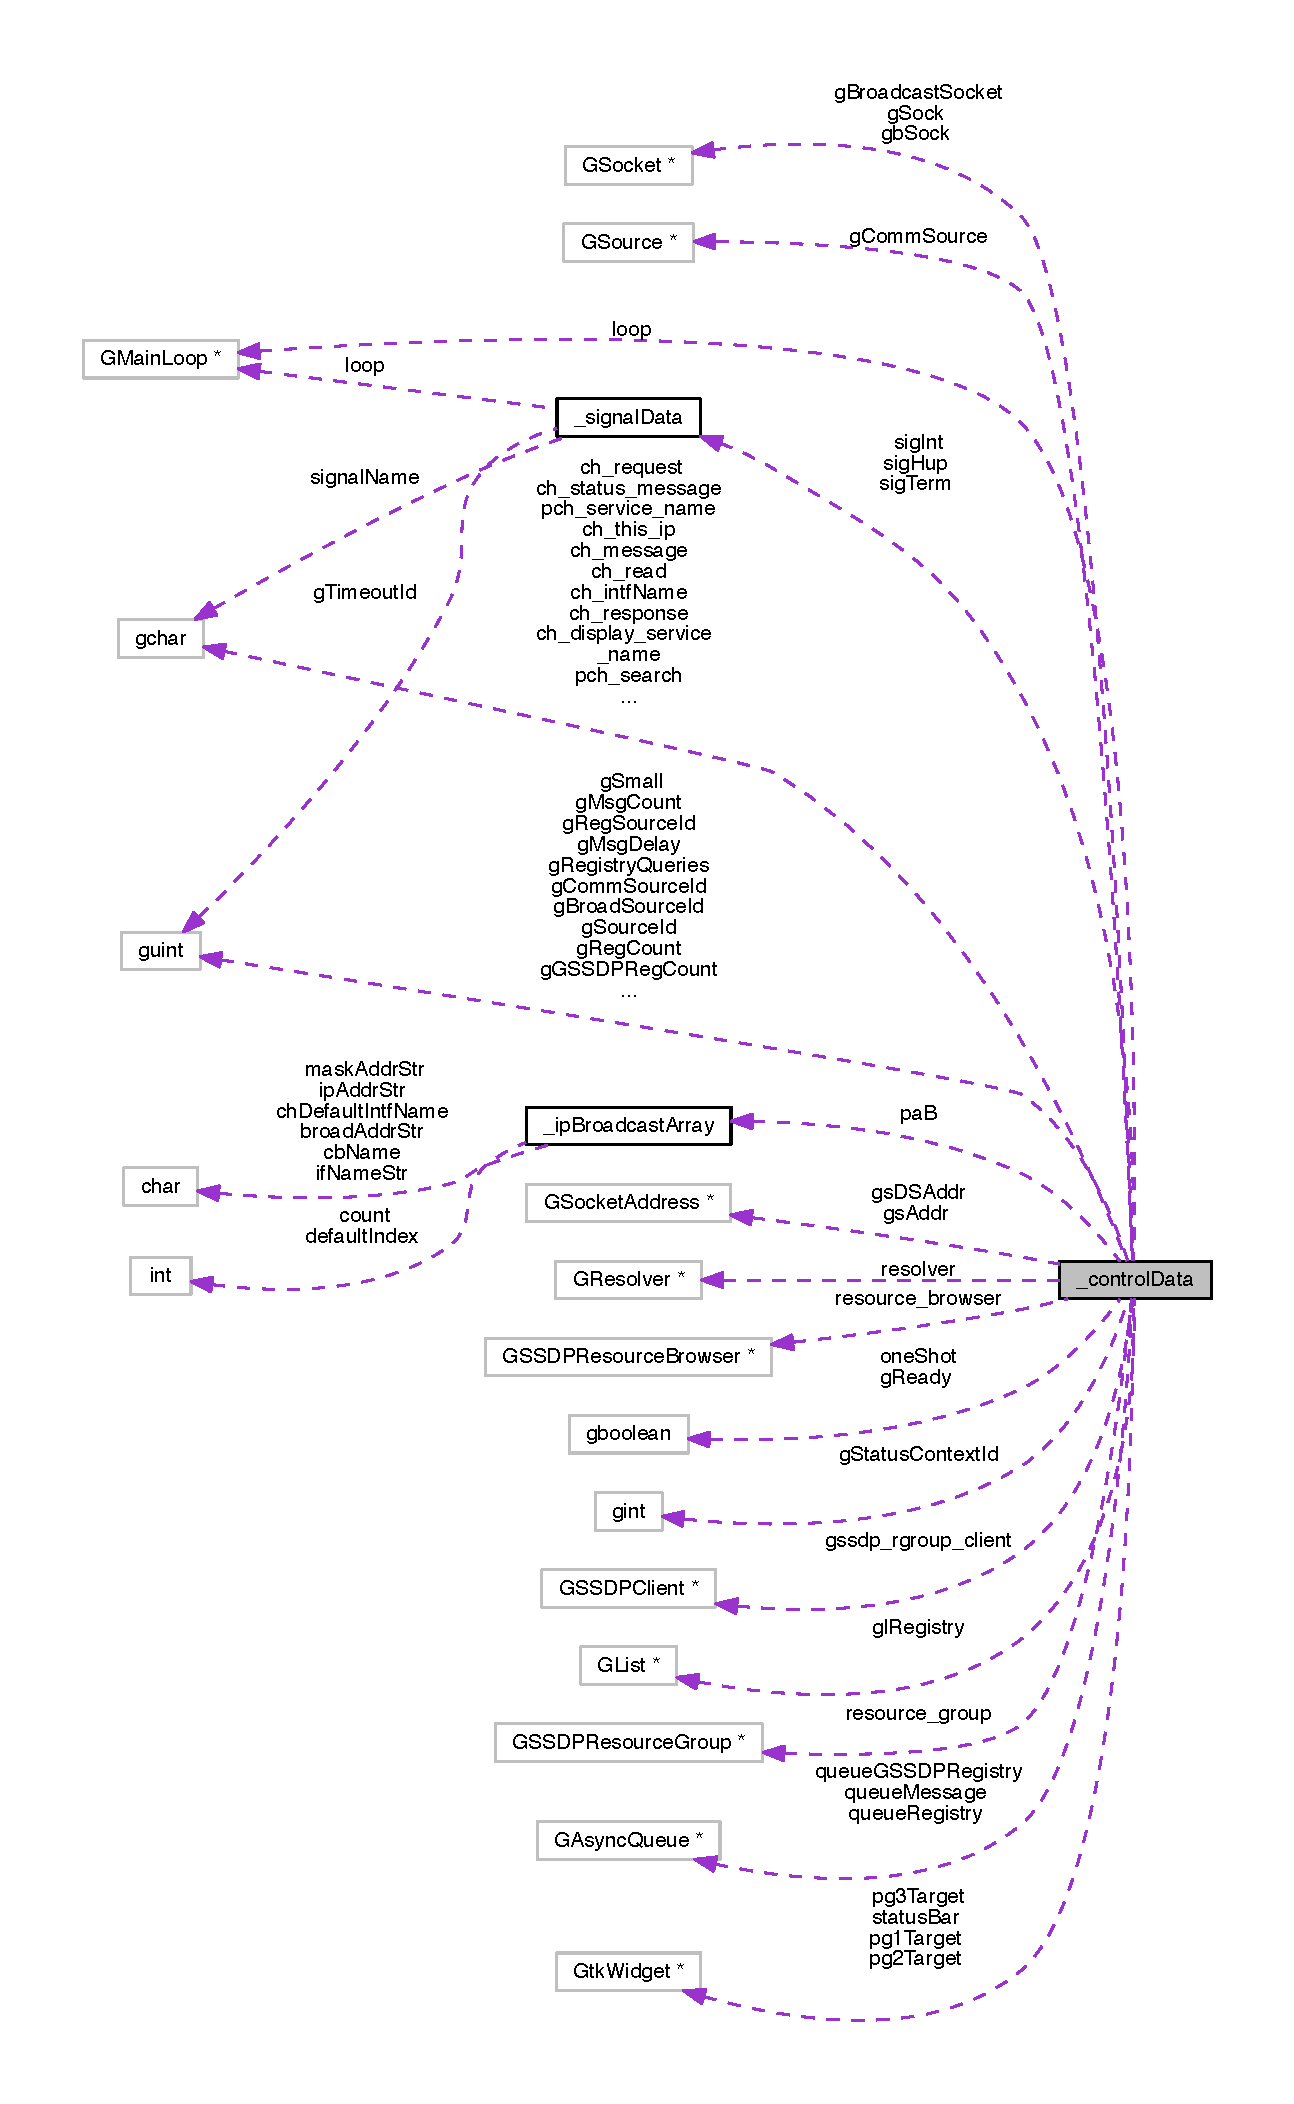
\includegraphics[height=550pt]{struct__control_data__coll__graph}
\end{center}
\end{figure}
\subsection*{Data Fields}
\begin{DoxyCompactItemize}
\item 
G\+Main\+Loop $\ast$ \hyperlink{struct__control_data_ae1b70bafbd5eb568c6ca339664959216}{loop}
\item 
\hyperlink{cmd_d_c_8c_a4d86cbb761613143e4ee60218efdfbaa}{U\+Signal\+Data} \hyperlink{struct__control_data_af45dc1f0c4806eaac0a57da17db50fdb}{sig\+Term}
\item 
\hyperlink{cmd_d_c_8c_a4d86cbb761613143e4ee60218efdfbaa}{U\+Signal\+Data} \hyperlink{struct__control_data_ae8ad5b5af46f4ab4bcd6ffb41e83385b}{sig\+Int}
\item 
\hyperlink{cmd_d_c_8c_a4d86cbb761613143e4ee60218efdfbaa}{U\+Signal\+Data} \hyperlink{struct__control_data_a551d0ecd4ceb9fc4ce8eebe5a984dc4c}{sig\+Hup}
\item 
G\+Source $\ast$ \hyperlink{struct__control_data_abfbd9e642ba240fa5985f63d60886de4}{g\+Comm\+Source}
\item 
G\+Socket $\ast$ \hyperlink{struct__control_data_a49b267275036fc3ac9b7d9e53b0625e1}{g\+Sock}
\item 
G\+Socket $\ast$ \hyperlink{struct__control_data_a05fab30fce92ebe541d9dd98220c60ef}{g\+Broadcast\+Socket}
\item 
G\+Socket\+Address $\ast$ \hyperlink{struct__control_data_a11c618822b208569a5d28206407326d5}{gs\+D\+S\+Addr}
\item 
G\+Socket\+Address $\ast$ \hyperlink{struct__control_data_a8a43853386551af4c746fd4b882eb2bf}{gs\+Addr}
\item 
G\+Resolver $\ast$ \hyperlink{struct__control_data_afe33a7083e1ecc9ba50a69644ed4a753}{resolver}
\item 
G\+List $\ast$ \hyperlink{struct__control_data_a34b1729bc0b37c9dce0327ea4cd8a812}{gl\+Registry}
\item 
\hyperlink{cmd_d_c_8c_a916d712cacebc2faeda930352280c361}{P\+I\+P\+Broadcast\+Array} \hyperlink{struct__control_data_a93f6e099a56c0d476607b4bd5a9dfa58}{pa\+B}
\item 
guint \hyperlink{struct__control_data_ab4837eb7cc16bf85fe0bd839a428eaa5}{g\+Registry\+Queries}
\item 
guint \hyperlink{struct__control_data_a81bfc0d50c23ebe6708e065659d11eb8}{g\+Reg\+Count}
\item 
guint \hyperlink{struct__control_data_a0dcc9f369186f6cf7c99b2178be66e58}{g\+Error\+Count}
\item 
guint \hyperlink{struct__control_data_a277ea878a8491fa38269b6c762a05389}{g\+Msg\+Delay}
\item 
gboolean \hyperlink{struct__control_data_a04238362a20b6616913d869fc464e4b2}{g\+Ready}
\item 
gchar \hyperlink{struct__control_data_adac6cf5482e4bbabb442f8ab27e4bc62}{ch\+\_\+intf\+Name} \mbox{[}\hyperlink{gtk_d_s_8c_a152ca8fa1a2eac39d1badafb6c6cef8c}{S\+Z\+\_\+\+R\+M\+T\+A\+D\+D\+R\+\_\+\+B\+U\+F\+F}\mbox{]}
\item 
gchar \hyperlink{struct__control_data_ac48fc4263dd4a6bad484b93fbf1ffe1b}{ch\+\_\+this\+\_\+ip} \mbox{[}\hyperlink{gtk_d_s_8c_a152ca8fa1a2eac39d1badafb6c6cef8c}{S\+Z\+\_\+\+R\+M\+T\+A\+D\+D\+R\+\_\+\+B\+U\+F\+F}\mbox{]}
\item 
gchar \hyperlink{struct__control_data_a94aa04264eafaa65a7a869a540bbdf93}{ch\+\_\+display\+\_\+service\+\_\+name} \mbox{[}\hyperlink{gtk_d_s_8c_a152ca8fa1a2eac39d1badafb6c6cef8c}{S\+Z\+\_\+\+R\+M\+T\+A\+D\+D\+R\+\_\+\+B\+U\+F\+F}\mbox{]}
\item 
gchar \hyperlink{struct__control_data_a16162d5fe851704d7ea50ff16525b94c}{ch\+\_\+message} \mbox{[}\hyperlink{gtk_d_s_8c_ab5903aa853c3769389e570c8490feb1e}{S\+Z\+\_\+\+M\+E\+S\+S\+A\+G\+E\+\_\+\+B\+U\+F\+F}\mbox{]}
\item 
gchar \hyperlink{struct__control_data_a948c37bbe26f5bdd4841b65384155edf}{ch\+\_\+request} \mbox{[}\hyperlink{gtk_d_s_8c_ab5903aa853c3769389e570c8490feb1e}{S\+Z\+\_\+\+M\+E\+S\+S\+A\+G\+E\+\_\+\+B\+U\+F\+F}\mbox{]}
\item 
gchar \hyperlink{struct__control_data_a9423e8582b05e2dde58b7302bee5559b}{ch\+\_\+response} \mbox{[}\hyperlink{gtk_d_s_8c_a3c73a8961a16a0dfbb87b5a7317bacd2}{S\+Z\+\_\+\+R\+E\+S\+P\+O\+N\+S\+E\+\_\+\+B\+U\+F\+F}\mbox{]}
\item 
guint \hyperlink{struct__control_data_a719187f5c3c94da5aa08616db7820b98}{g\+Source\+Id}
\item 
guint \hyperlink{struct__control_data_ae9e5e76959a76812d94ee8f83ae2eef5}{g\+Broad\+Source\+Id}
\item 
G\+Socket $\ast$ \hyperlink{struct__control_data_a3023250e01849cb311a7207746a3b64e}{gb\+Sock}
\item 
gchar \hyperlink{struct__control_data_a243b075becb92f2f37f56f60f738efb1}{ch\+\_\+read} \mbox{[}\hyperlink{gtk_d_s_8c_ab5903aa853c3769389e570c8490feb1e}{S\+Z\+\_\+\+M\+E\+S\+S\+A\+G\+E\+\_\+\+B\+U\+F\+F}\mbox{]}
\item 
gchar $\ast$ \hyperlink{struct__control_data_a2197fd3d9315510193866dbedbd3cc8b}{pch\+\_\+service\+\_\+name}
\item 
guint \hyperlink{struct__control_data_a78b36762a9d85d027fc5e41576ade4f7}{g\+U\+D\+P\+Port}
\item 
G\+S\+S\+D\+P\+Client $\ast$ \hyperlink{struct__control_data_a05dec2c5c598d299306a41430093b6de}{gssdp\+\_\+rgroup\+\_\+client}
\item 
G\+S\+S\+D\+P\+Resource\+Browser $\ast$ \hyperlink{struct__control_data_a796910b4ad0830538301efd69811c2c6}{resource\+\_\+browser}
\item 
gboolean \hyperlink{struct__control_data_a772b5b4e4d92eee73100445963cbe682}{one\+Shot}
\item 
gchar $\ast$ \hyperlink{struct__control_data_aae1d10aba11260e77341d9f5fa6055e2}{pch\+\_\+search}
\item 
guint \hyperlink{struct__control_data_a4be65550b087ca645572b8ebc726250d}{g\+Msg\+Source\+Id}
\item 
guint \hyperlink{struct__control_data_a96ccde7cdcba6f4f52f472f95ddaf782}{g\+Reg\+Source\+Id}
\item 
guint \hyperlink{struct__control_data_a599cefa2edf28b0cf58f9180a3be0a19}{g\+Comm\+Source\+Id}
\item 
guint \hyperlink{struct__control_data_a4132cf34364874408e8b15be539e654d}{g\+G\+S\+S\+D\+P\+Reg\+Source\+Id}
\item 
guint \hyperlink{struct__control_data_ae797898f8e5ad5c3128da674f86520d1}{g\+Msg\+Count}
\item 
guint \hyperlink{struct__control_data_a841eb51dde0376a7540a23e65933e822}{g\+G\+S\+S\+D\+P\+Reg\+Count}
\item 
gint \hyperlink{struct__control_data_aae36ce9466663c5765139bb92e9f8d49}{g\+Status\+Context\+Id}
\item 
guint \hyperlink{struct__control_data_aa53ce6d64a23cb93cc0c98e0835b6449}{g\+Small}
\item 
G\+S\+S\+D\+P\+Resource\+Group $\ast$ \hyperlink{struct__control_data_ab8684a42dc1f2e00247d7278d47046b9}{resource\+\_\+group}
\item 
G\+Async\+Queue $\ast$ \hyperlink{struct__control_data_adc74ddf3f6a7535eee87d39ed80ee7dd}{queue\+Message}
\item 
G\+Async\+Queue $\ast$ \hyperlink{struct__control_data_a09b9467cd00be5a9ecac2386429ab65a}{queue\+Registry}
\item 
G\+Async\+Queue $\ast$ \hyperlink{struct__control_data_ad4c1f099018b51b0faeae870d284819d}{queue\+G\+S\+S\+D\+P\+Registry}
\item 
Gtk\+Widget $\ast$ \hyperlink{struct__control_data_a661ed960369e640e5f56da1abe7c2168}{status\+Bar}
\item 
Gtk\+Widget $\ast$ \hyperlink{struct__control_data_adb6c2830054c6309779d676082e94447}{pg1\+Target}
\item 
Gtk\+Widget $\ast$ \hyperlink{struct__control_data_a201f826ab99699df83a85c5e4572ffb2}{pg2\+Target}
\item 
Gtk\+Widget $\ast$ \hyperlink{struct__control_data_a67d45a0e9ba1fcaabea3600dfee830b9}{pg3\+Target}
\item 
gchar \hyperlink{struct__control_data_aa6d5e703090d185edd3e0b5224542ce5}{ch\+\_\+status\+\_\+message} \mbox{[}\hyperlink{gtk_d_s_8c_ab5903aa853c3769389e570c8490feb1e}{S\+Z\+\_\+\+M\+E\+S\+S\+A\+G\+E\+\_\+\+B\+U\+F\+F}\mbox{]}
\end{DoxyCompactItemize}


\subsection{Detailed Description}


Definition at line 90 of file cmd\+D\+C.\+c.



\subsection{Field Documentation}
\hypertarget{struct__control_data_a94aa04264eafaa65a7a869a540bbdf93}{\index{\+\_\+control\+Data@{\+\_\+control\+Data}!ch\+\_\+display\+\_\+service\+\_\+name@{ch\+\_\+display\+\_\+service\+\_\+name}}
\index{ch\+\_\+display\+\_\+service\+\_\+name@{ch\+\_\+display\+\_\+service\+\_\+name}!\+\_\+control\+Data@{\+\_\+control\+Data}}
\subsubsection[{ch\+\_\+display\+\_\+service\+\_\+name}]{\setlength{\rightskip}{0pt plus 5cm}gchar \+\_\+control\+Data\+::ch\+\_\+display\+\_\+service\+\_\+name}}\label{struct__control_data_a94aa04264eafaa65a7a869a540bbdf93}


Definition at line 110 of file cmd\+D\+C.\+c.



Referenced by cb\+\_\+udp\+\_\+broadcast\+\_\+response\+\_\+handler(), cb\+\_\+udp\+\_\+comm\+\_\+request\+\_\+handler(), cb\+\_\+udp\+\_\+registry\+\_\+select\+\_\+handler(), and main().

\hypertarget{struct__control_data_adac6cf5482e4bbabb442f8ab27e4bc62}{\index{\+\_\+control\+Data@{\+\_\+control\+Data}!ch\+\_\+intf\+Name@{ch\+\_\+intf\+Name}}
\index{ch\+\_\+intf\+Name@{ch\+\_\+intf\+Name}!\+\_\+control\+Data@{\+\_\+control\+Data}}
\subsubsection[{ch\+\_\+intf\+Name}]{\setlength{\rightskip}{0pt plus 5cm}gchar \+\_\+control\+Data\+::ch\+\_\+intf\+Name}}\label{struct__control_data_adac6cf5482e4bbabb442f8ab27e4bc62}


Definition at line 108 of file cmd\+D\+C.\+c.



Referenced by main().

\hypertarget{struct__control_data_a16162d5fe851704d7ea50ff16525b94c}{\index{\+\_\+control\+Data@{\+\_\+control\+Data}!ch\+\_\+message@{ch\+\_\+message}}
\index{ch\+\_\+message@{ch\+\_\+message}!\+\_\+control\+Data@{\+\_\+control\+Data}}
\subsubsection[{ch\+\_\+message}]{\setlength{\rightskip}{0pt plus 5cm}gchar \+\_\+control\+Data\+::ch\+\_\+message}}\label{struct__control_data_a16162d5fe851704d7ea50ff16525b94c}


Definition at line 111 of file cmd\+D\+C.\+c.



Referenced by cb\+\_\+udp\+\_\+comm\+\_\+request\+\_\+handler(), and main().

\hypertarget{struct__control_data_a243b075becb92f2f37f56f60f738efb1}{\index{\+\_\+control\+Data@{\+\_\+control\+Data}!ch\+\_\+read@{ch\+\_\+read}}
\index{ch\+\_\+read@{ch\+\_\+read}!\+\_\+control\+Data@{\+\_\+control\+Data}}
\subsubsection[{ch\+\_\+read}]{\setlength{\rightskip}{0pt plus 5cm}gchar \+\_\+control\+Data\+::ch\+\_\+read\mbox{[}{\bf S\+Z\+\_\+\+M\+E\+S\+S\+A\+G\+E\+\_\+\+B\+U\+F\+F}\mbox{]}}}\label{struct__control_data_a243b075becb92f2f37f56f60f738efb1}


Definition at line 96 of file cmd\+D\+S.\+c.



Referenced by cb\+\_\+udp\+\_\+request\+\_\+handler().

\hypertarget{struct__control_data_a948c37bbe26f5bdd4841b65384155edf}{\index{\+\_\+control\+Data@{\+\_\+control\+Data}!ch\+\_\+request@{ch\+\_\+request}}
\index{ch\+\_\+request@{ch\+\_\+request}!\+\_\+control\+Data@{\+\_\+control\+Data}}
\subsubsection[{ch\+\_\+request}]{\setlength{\rightskip}{0pt plus 5cm}gchar \+\_\+control\+Data\+::ch\+\_\+request}}\label{struct__control_data_a948c37bbe26f5bdd4841b65384155edf}


Definition at line 112 of file cmd\+D\+C.\+c.



Referenced by cb\+\_\+udp\+\_\+comm\+\_\+response\+\_\+handler(), and cb\+\_\+udp\+\_\+request\+\_\+handler().

\hypertarget{struct__control_data_a9423e8582b05e2dde58b7302bee5559b}{\index{\+\_\+control\+Data@{\+\_\+control\+Data}!ch\+\_\+response@{ch\+\_\+response}}
\index{ch\+\_\+response@{ch\+\_\+response}!\+\_\+control\+Data@{\+\_\+control\+Data}}
\subsubsection[{ch\+\_\+response}]{\setlength{\rightskip}{0pt plus 5cm}gchar \+\_\+control\+Data\+::ch\+\_\+response}}\label{struct__control_data_a9423e8582b05e2dde58b7302bee5559b}


Definition at line 113 of file cmd\+D\+C.\+c.



Referenced by cb\+\_\+udp\+\_\+comm\+\_\+response\+\_\+handler(), and cb\+\_\+udp\+\_\+request\+\_\+handler().

\hypertarget{struct__control_data_aa6d5e703090d185edd3e0b5224542ce5}{\index{\+\_\+control\+Data@{\+\_\+control\+Data}!ch\+\_\+status\+\_\+message@{ch\+\_\+status\+\_\+message}}
\index{ch\+\_\+status\+\_\+message@{ch\+\_\+status\+\_\+message}!\+\_\+control\+Data@{\+\_\+control\+Data}}
\subsubsection[{ch\+\_\+status\+\_\+message}]{\setlength{\rightskip}{0pt plus 5cm}gchar \+\_\+control\+Data\+::ch\+\_\+status\+\_\+message\mbox{[}{\bf S\+Z\+\_\+\+M\+E\+S\+S\+A\+G\+E\+\_\+\+B\+U\+F\+F}\mbox{]}}}\label{struct__control_data_aa6d5e703090d185edd3e0b5224542ce5}


Definition at line 141 of file gtk\+D\+S.\+c.

\hypertarget{struct__control_data_ac48fc4263dd4a6bad484b93fbf1ffe1b}{\index{\+\_\+control\+Data@{\+\_\+control\+Data}!ch\+\_\+this\+\_\+ip@{ch\+\_\+this\+\_\+ip}}
\index{ch\+\_\+this\+\_\+ip@{ch\+\_\+this\+\_\+ip}!\+\_\+control\+Data@{\+\_\+control\+Data}}
\subsubsection[{ch\+\_\+this\+\_\+ip}]{\setlength{\rightskip}{0pt plus 5cm}gchar \+\_\+control\+Data\+::ch\+\_\+this\+\_\+ip}}\label{struct__control_data_ac48fc4263dd4a6bad484b93fbf1ffe1b}


Definition at line 109 of file cmd\+D\+C.\+c.



Referenced by cb\+\_\+udp\+\_\+broadcast\+\_\+response\+\_\+handler(), gssdp\+\_\+publish(), and main().

\hypertarget{struct__control_data_a05fab30fce92ebe541d9dd98220c60ef}{\index{\+\_\+control\+Data@{\+\_\+control\+Data}!g\+Broadcast\+Socket@{g\+Broadcast\+Socket}}
\index{g\+Broadcast\+Socket@{g\+Broadcast\+Socket}!\+\_\+control\+Data@{\+\_\+control\+Data}}
\subsubsection[{g\+Broadcast\+Socket}]{\setlength{\rightskip}{0pt plus 5cm}G\+Socket$\ast$ \+\_\+control\+Data\+::g\+Broadcast\+Socket}}\label{struct__control_data_a05fab30fce92ebe541d9dd98220c60ef}


Definition at line 97 of file cmd\+D\+C.\+c.



Referenced by cb\+\_\+udp\+\_\+registry\+\_\+select\+\_\+handler(), and main().

\hypertarget{struct__control_data_ae9e5e76959a76812d94ee8f83ae2eef5}{\index{\+\_\+control\+Data@{\+\_\+control\+Data}!g\+Broad\+Source\+Id@{g\+Broad\+Source\+Id}}
\index{g\+Broad\+Source\+Id@{g\+Broad\+Source\+Id}!\+\_\+control\+Data@{\+\_\+control\+Data}}
\subsubsection[{g\+Broad\+Source\+Id}]{\setlength{\rightskip}{0pt plus 5cm}guint \+\_\+control\+Data\+::g\+Broad\+Source\+Id}}\label{struct__control_data_ae9e5e76959a76812d94ee8f83ae2eef5}


Definition at line 91 of file cmd\+D\+S.\+c.



Referenced by main().

\hypertarget{struct__control_data_a3023250e01849cb311a7207746a3b64e}{\index{\+\_\+control\+Data@{\+\_\+control\+Data}!gb\+Sock@{gb\+Sock}}
\index{gb\+Sock@{gb\+Sock}!\+\_\+control\+Data@{\+\_\+control\+Data}}
\subsubsection[{gb\+Sock}]{\setlength{\rightskip}{0pt plus 5cm}G\+Socket $\ast$ \+\_\+control\+Data\+::gb\+Sock}}\label{struct__control_data_a3023250e01849cb311a7207746a3b64e}


Definition at line 95 of file cmd\+D\+S.\+c.



Referenced by cb\+\_\+registry\+\_\+refresh(), and main().

\hypertarget{struct__control_data_abfbd9e642ba240fa5985f63d60886de4}{\index{\+\_\+control\+Data@{\+\_\+control\+Data}!g\+Comm\+Source@{g\+Comm\+Source}}
\index{g\+Comm\+Source@{g\+Comm\+Source}!\+\_\+control\+Data@{\+\_\+control\+Data}}
\subsubsection[{g\+Comm\+Source}]{\setlength{\rightskip}{0pt plus 5cm}G\+Source $\ast$ \+\_\+control\+Data\+::g\+Comm\+Source}}\label{struct__control_data_abfbd9e642ba240fa5985f63d60886de4}


Definition at line 95 of file cmd\+D\+C.\+c.



Referenced by main(), and udp\+\_\+initialize\+\_\+message\+\_\+send().

\hypertarget{struct__control_data_a599cefa2edf28b0cf58f9180a3be0a19}{\index{\+\_\+control\+Data@{\+\_\+control\+Data}!g\+Comm\+Source\+Id@{g\+Comm\+Source\+Id}}
\index{g\+Comm\+Source\+Id@{g\+Comm\+Source\+Id}!\+\_\+control\+Data@{\+\_\+control\+Data}}
\subsubsection[{g\+Comm\+Source\+Id}]{\setlength{\rightskip}{0pt plus 5cm}guint \+\_\+control\+Data\+::g\+Comm\+Source\+Id}}\label{struct__control_data_a599cefa2edf28b0cf58f9180a3be0a19}


Definition at line 116 of file gtk\+D\+S.\+c.



Referenced by main().

\hypertarget{struct__control_data_a0dcc9f369186f6cf7c99b2178be66e58}{\index{\+\_\+control\+Data@{\+\_\+control\+Data}!g\+Error\+Count@{g\+Error\+Count}}
\index{g\+Error\+Count@{g\+Error\+Count}!\+\_\+control\+Data@{\+\_\+control\+Data}}
\subsubsection[{g\+Error\+Count}]{\setlength{\rightskip}{0pt plus 5cm}guint \+\_\+control\+Data\+::g\+Error\+Count}}\label{struct__control_data_a0dcc9f369186f6cf7c99b2178be66e58}


Definition at line 105 of file cmd\+D\+C.\+c.



Referenced by cb\+\_\+udp\+\_\+comm\+\_\+request\+\_\+handler(), cb\+\_\+udp\+\_\+comm\+\_\+response\+\_\+handler(), and main().

\hypertarget{struct__control_data_a841eb51dde0376a7540a23e65933e822}{\index{\+\_\+control\+Data@{\+\_\+control\+Data}!g\+G\+S\+S\+D\+P\+Reg\+Count@{g\+G\+S\+S\+D\+P\+Reg\+Count}}
\index{g\+G\+S\+S\+D\+P\+Reg\+Count@{g\+G\+S\+S\+D\+P\+Reg\+Count}!\+\_\+control\+Data@{\+\_\+control\+Data}}
\subsubsection[{g\+G\+S\+S\+D\+P\+Reg\+Count}]{\setlength{\rightskip}{0pt plus 5cm}guint \+\_\+control\+Data\+::g\+G\+S\+S\+D\+P\+Reg\+Count}}\label{struct__control_data_a841eb51dde0376a7540a23e65933e822}


Definition at line 120 of file gtk\+D\+S.\+c.



Referenced by cb\+\_\+gssdp\+\_\+registry\+\_\+request\+\_\+handler(), main(), and ui\+\_\+update\+\_\+status\+\_\+bar().

\hypertarget{struct__control_data_a4132cf34364874408e8b15be539e654d}{\index{\+\_\+control\+Data@{\+\_\+control\+Data}!g\+G\+S\+S\+D\+P\+Reg\+Source\+Id@{g\+G\+S\+S\+D\+P\+Reg\+Source\+Id}}
\index{g\+G\+S\+S\+D\+P\+Reg\+Source\+Id@{g\+G\+S\+S\+D\+P\+Reg\+Source\+Id}!\+\_\+control\+Data@{\+\_\+control\+Data}}
\subsubsection[{g\+G\+S\+S\+D\+P\+Reg\+Source\+Id}]{\setlength{\rightskip}{0pt plus 5cm}guint \+\_\+control\+Data\+::g\+G\+S\+S\+D\+P\+Reg\+Source\+Id}}\label{struct__control_data_a4132cf34364874408e8b15be539e654d}


Definition at line 118 of file gtk\+D\+S.\+c.



Referenced by main().

\hypertarget{struct__control_data_a34b1729bc0b37c9dce0327ea4cd8a812}{\index{\+\_\+control\+Data@{\+\_\+control\+Data}!gl\+Registry@{gl\+Registry}}
\index{gl\+Registry@{gl\+Registry}!\+\_\+control\+Data@{\+\_\+control\+Data}}
\subsubsection[{gl\+Registry}]{\setlength{\rightskip}{0pt plus 5cm}G\+List $\ast$ \+\_\+control\+Data\+::gl\+Registry}}\label{struct__control_data_a34b1729bc0b37c9dce0327ea4cd8a812}


Definition at line 101 of file cmd\+D\+C.\+c.



Referenced by cb\+\_\+gssdp\+\_\+resource\+\_\+available(), cb\+\_\+udp\+\_\+broadcast\+\_\+response\+\_\+handler(), cb\+\_\+udp\+\_\+registry\+\_\+select\+\_\+handler(), and main().

\hypertarget{struct__control_data_ae797898f8e5ad5c3128da674f86520d1}{\index{\+\_\+control\+Data@{\+\_\+control\+Data}!g\+Msg\+Count@{g\+Msg\+Count}}
\index{g\+Msg\+Count@{g\+Msg\+Count}!\+\_\+control\+Data@{\+\_\+control\+Data}}
\subsubsection[{g\+Msg\+Count}]{\setlength{\rightskip}{0pt plus 5cm}guint \+\_\+control\+Data\+::g\+Msg\+Count}}\label{struct__control_data_ae797898f8e5ad5c3128da674f86520d1}


Definition at line 119 of file gtk\+D\+S.\+c.



Referenced by cb\+\_\+message\+\_\+request\+\_\+handler(), main(), and ui\+\_\+update\+\_\+status\+\_\+bar().

\hypertarget{struct__control_data_a277ea878a8491fa38269b6c762a05389}{\index{\+\_\+control\+Data@{\+\_\+control\+Data}!g\+Msg\+Delay@{g\+Msg\+Delay}}
\index{g\+Msg\+Delay@{g\+Msg\+Delay}!\+\_\+control\+Data@{\+\_\+control\+Data}}
\subsubsection[{g\+Msg\+Delay}]{\setlength{\rightskip}{0pt plus 5cm}guint \+\_\+control\+Data\+::g\+Msg\+Delay}}\label{struct__control_data_a277ea878a8491fa38269b6c762a05389}


Definition at line 106 of file cmd\+D\+C.\+c.



Referenced by cb\+\_\+udp\+\_\+registry\+\_\+select\+\_\+handler(), main(), and udp\+\_\+initialize\+\_\+message\+\_\+send().

\hypertarget{struct__control_data_a4be65550b087ca645572b8ebc726250d}{\index{\+\_\+control\+Data@{\+\_\+control\+Data}!g\+Msg\+Source\+Id@{g\+Msg\+Source\+Id}}
\index{g\+Msg\+Source\+Id@{g\+Msg\+Source\+Id}!\+\_\+control\+Data@{\+\_\+control\+Data}}
\subsubsection[{g\+Msg\+Source\+Id}]{\setlength{\rightskip}{0pt plus 5cm}guint \+\_\+control\+Data\+::g\+Msg\+Source\+Id}}\label{struct__control_data_a4be65550b087ca645572b8ebc726250d}


Definition at line 114 of file gtk\+D\+S.\+c.



Referenced by main().

\hypertarget{struct__control_data_a04238362a20b6616913d869fc464e4b2}{\index{\+\_\+control\+Data@{\+\_\+control\+Data}!g\+Ready@{g\+Ready}}
\index{g\+Ready@{g\+Ready}!\+\_\+control\+Data@{\+\_\+control\+Data}}
\subsubsection[{g\+Ready}]{\setlength{\rightskip}{0pt plus 5cm}gboolean \+\_\+control\+Data\+::g\+Ready}}\label{struct__control_data_a04238362a20b6616913d869fc464e4b2}


Definition at line 107 of file cmd\+D\+C.\+c.



Referenced by cb\+\_\+udp\+\_\+registry\+\_\+select\+\_\+handler(), and main().

\hypertarget{struct__control_data_a81bfc0d50c23ebe6708e065659d11eb8}{\index{\+\_\+control\+Data@{\+\_\+control\+Data}!g\+Reg\+Count@{g\+Reg\+Count}}
\index{g\+Reg\+Count@{g\+Reg\+Count}!\+\_\+control\+Data@{\+\_\+control\+Data}}
\subsubsection[{g\+Reg\+Count}]{\setlength{\rightskip}{0pt plus 5cm}guint \+\_\+control\+Data\+::g\+Reg\+Count}}\label{struct__control_data_a81bfc0d50c23ebe6708e065659d11eb8}


Definition at line 104 of file cmd\+D\+C.\+c.



Referenced by cb\+\_\+registry\+\_\+request\+\_\+handler(), main(), and ui\+\_\+update\+\_\+status\+\_\+bar().

\hypertarget{struct__control_data_ab4837eb7cc16bf85fe0bd839a428eaa5}{\index{\+\_\+control\+Data@{\+\_\+control\+Data}!g\+Registry\+Queries@{g\+Registry\+Queries}}
\index{g\+Registry\+Queries@{g\+Registry\+Queries}!\+\_\+control\+Data@{\+\_\+control\+Data}}
\subsubsection[{g\+Registry\+Queries}]{\setlength{\rightskip}{0pt plus 5cm}guint \+\_\+control\+Data\+::g\+Registry\+Queries}}\label{struct__control_data_ab4837eb7cc16bf85fe0bd839a428eaa5}


Definition at line 103 of file cmd\+D\+C.\+c.



Referenced by cb\+\_\+udp\+\_\+registry\+\_\+select\+\_\+handler(), and main().

\hypertarget{struct__control_data_a96ccde7cdcba6f4f52f472f95ddaf782}{\index{\+\_\+control\+Data@{\+\_\+control\+Data}!g\+Reg\+Source\+Id@{g\+Reg\+Source\+Id}}
\index{g\+Reg\+Source\+Id@{g\+Reg\+Source\+Id}!\+\_\+control\+Data@{\+\_\+control\+Data}}
\subsubsection[{g\+Reg\+Source\+Id}]{\setlength{\rightskip}{0pt plus 5cm}guint \+\_\+control\+Data\+::g\+Reg\+Source\+Id}}\label{struct__control_data_a96ccde7cdcba6f4f52f472f95ddaf782}


Definition at line 115 of file gtk\+D\+S.\+c.



Referenced by main().

\hypertarget{struct__control_data_a8a43853386551af4c746fd4b882eb2bf}{\index{\+\_\+control\+Data@{\+\_\+control\+Data}!gs\+Addr@{gs\+Addr}}
\index{gs\+Addr@{gs\+Addr}!\+\_\+control\+Data@{\+\_\+control\+Data}}
\subsubsection[{gs\+Addr}]{\setlength{\rightskip}{0pt plus 5cm}G\+Socket\+Address $\ast$ \+\_\+control\+Data\+::gs\+Addr}}\label{struct__control_data_a8a43853386551af4c746fd4b882eb2bf}


Definition at line 99 of file cmd\+D\+C.\+c.



Referenced by main(), and udp\+\_\+initialize\+\_\+message\+\_\+send().

\hypertarget{struct__control_data_a11c618822b208569a5d28206407326d5}{\index{\+\_\+control\+Data@{\+\_\+control\+Data}!gs\+D\+S\+Addr@{gs\+D\+S\+Addr}}
\index{gs\+D\+S\+Addr@{gs\+D\+S\+Addr}!\+\_\+control\+Data@{\+\_\+control\+Data}}
\subsubsection[{gs\+D\+S\+Addr}]{\setlength{\rightskip}{0pt plus 5cm}G\+Socket\+Address $\ast$ \+\_\+control\+Data\+::gs\+D\+S\+Addr}}\label{struct__control_data_a11c618822b208569a5d28206407326d5}


Definition at line 98 of file cmd\+D\+C.\+c.



Referenced by cb\+\_\+udp\+\_\+comm\+\_\+request\+\_\+handler(), cb\+\_\+udp\+\_\+registry\+\_\+select\+\_\+handler(), and main().

\hypertarget{struct__control_data_aa53ce6d64a23cb93cc0c98e0835b6449}{\index{\+\_\+control\+Data@{\+\_\+control\+Data}!g\+Small@{g\+Small}}
\index{g\+Small@{g\+Small}!\+\_\+control\+Data@{\+\_\+control\+Data}}
\subsubsection[{g\+Small}]{\setlength{\rightskip}{0pt plus 5cm}guint \+\_\+control\+Data\+::g\+Small}}\label{struct__control_data_aa53ce6d64a23cb93cc0c98e0835b6449}


Definition at line 124 of file gtk\+D\+S.\+c.



Referenced by main(), ui\+\_\+page\+\_\+layout(), and ui\+\_\+update\+\_\+status\+\_\+bar().

\hypertarget{struct__control_data_a49b267275036fc3ac9b7d9e53b0625e1}{\index{\+\_\+control\+Data@{\+\_\+control\+Data}!g\+Sock@{g\+Sock}}
\index{g\+Sock@{g\+Sock}!\+\_\+control\+Data@{\+\_\+control\+Data}}
\subsubsection[{g\+Sock}]{\setlength{\rightskip}{0pt plus 5cm}G\+Socket $\ast$ \+\_\+control\+Data\+::g\+Sock}}\label{struct__control_data_a49b267275036fc3ac9b7d9e53b0625e1}


Definition at line 96 of file cmd\+D\+C.\+c.



Referenced by cb\+\_\+udp\+\_\+comm\+\_\+request\+\_\+handler(), main(), and udp\+\_\+initialize\+\_\+message\+\_\+send().

\hypertarget{struct__control_data_a719187f5c3c94da5aa08616db7820b98}{\index{\+\_\+control\+Data@{\+\_\+control\+Data}!g\+Source\+Id@{g\+Source\+Id}}
\index{g\+Source\+Id@{g\+Source\+Id}!\+\_\+control\+Data@{\+\_\+control\+Data}}
\subsubsection[{g\+Source\+Id}]{\setlength{\rightskip}{0pt plus 5cm}guint \+\_\+control\+Data\+::g\+Source\+Id}}\label{struct__control_data_a719187f5c3c94da5aa08616db7820b98}


Definition at line 90 of file cmd\+D\+S.\+c.



Referenced by main().

\hypertarget{struct__control_data_a05dec2c5c598d299306a41430093b6de}{\index{\+\_\+control\+Data@{\+\_\+control\+Data}!gssdp\+\_\+rgroup\+\_\+client@{gssdp\+\_\+rgroup\+\_\+client}}
\index{gssdp\+\_\+rgroup\+\_\+client@{gssdp\+\_\+rgroup\+\_\+client}!\+\_\+control\+Data@{\+\_\+control\+Data}}
\subsubsection[{gssdp\+\_\+rgroup\+\_\+client}]{\setlength{\rightskip}{0pt plus 5cm}G\+S\+S\+D\+P\+Client $\ast$ \+\_\+control\+Data\+::gssdp\+\_\+rgroup\+\_\+client}}\label{struct__control_data_a05dec2c5c598d299306a41430093b6de}


Definition at line 107 of file gssdp\+D\+C.\+c.



Referenced by gssdp\+\_\+browse(), gssdp\+\_\+publish(), main(), and skn\+\_\+gssdp\+\_\+browse().

\hypertarget{struct__control_data_aae36ce9466663c5765139bb92e9f8d49}{\index{\+\_\+control\+Data@{\+\_\+control\+Data}!g\+Status\+Context\+Id@{g\+Status\+Context\+Id}}
\index{g\+Status\+Context\+Id@{g\+Status\+Context\+Id}!\+\_\+control\+Data@{\+\_\+control\+Data}}
\subsubsection[{g\+Status\+Context\+Id}]{\setlength{\rightskip}{0pt plus 5cm}gint \+\_\+control\+Data\+::g\+Status\+Context\+Id}}\label{struct__control_data_aae36ce9466663c5765139bb92e9f8d49}


Definition at line 122 of file gtk\+D\+S.\+c.



Referenced by ui\+\_\+page\+\_\+layout(), and ui\+\_\+update\+\_\+status\+\_\+bar().

\hypertarget{struct__control_data_a78b36762a9d85d027fc5e41576ade4f7}{\index{\+\_\+control\+Data@{\+\_\+control\+Data}!g\+U\+D\+P\+Port@{g\+U\+D\+P\+Port}}
\index{g\+U\+D\+P\+Port@{g\+U\+D\+P\+Port}!\+\_\+control\+Data@{\+\_\+control\+Data}}
\subsubsection[{g\+U\+D\+P\+Port}]{\setlength{\rightskip}{0pt plus 5cm}guint \+\_\+control\+Data\+::g\+U\+D\+P\+Port}}\label{struct__control_data_a78b36762a9d85d027fc5e41576ade4f7}


Definition at line 102 of file cmd\+D\+S.\+c.



Referenced by cb\+\_\+udp\+\_\+broadcast\+\_\+response\+\_\+handler(), and main().

\hypertarget{struct__control_data_ae1b70bafbd5eb568c6ca339664959216}{\index{\+\_\+control\+Data@{\+\_\+control\+Data}!loop@{loop}}
\index{loop@{loop}!\+\_\+control\+Data@{\+\_\+control\+Data}}
\subsubsection[{loop}]{\setlength{\rightskip}{0pt plus 5cm}G\+Main\+Loop $\ast$ \+\_\+control\+Data\+::loop}}\label{struct__control_data_ae1b70bafbd5eb568c6ca339664959216}


Definition at line 91 of file cmd\+D\+C.\+c.



Referenced by cb\+\_\+udp\+\_\+broadcast\+\_\+response\+\_\+handler(), cb\+\_\+udp\+\_\+comm\+\_\+request\+\_\+handler(), cb\+\_\+udp\+\_\+comm\+\_\+response\+\_\+handler(), cb\+\_\+udp\+\_\+request\+\_\+handler(), and main().

\hypertarget{struct__control_data_a772b5b4e4d92eee73100445963cbe682}{\index{\+\_\+control\+Data@{\+\_\+control\+Data}!one\+Shot@{one\+Shot}}
\index{one\+Shot@{one\+Shot}!\+\_\+control\+Data@{\+\_\+control\+Data}}
\subsubsection[{one\+Shot}]{\setlength{\rightskip}{0pt plus 5cm}gboolean \+\_\+control\+Data\+::one\+Shot}}\label{struct__control_data_a772b5b4e4d92eee73100445963cbe682}


Definition at line 117 of file gssdp\+D\+C.\+c.



Referenced by cb\+\_\+udp\+\_\+comm\+\_\+response\+\_\+handler(), and main().

\hypertarget{struct__control_data_a93f6e099a56c0d476607b4bd5a9dfa58}{\index{\+\_\+control\+Data@{\+\_\+control\+Data}!pa\+B@{pa\+B}}
\index{pa\+B@{pa\+B}!\+\_\+control\+Data@{\+\_\+control\+Data}}
\subsubsection[{pa\+B}]{\setlength{\rightskip}{0pt plus 5cm}{\bf P\+I\+P\+Broadcast\+Array} \+\_\+control\+Data\+::pa\+B}}\label{struct__control_data_a93f6e099a56c0d476607b4bd5a9dfa58}


Definition at line 102 of file cmd\+D\+C.\+c.



Referenced by cb\+\_\+registry\+\_\+refresh(), cb\+\_\+udp\+\_\+registry\+\_\+select\+\_\+handler(), and main().

\hypertarget{struct__control_data_aae1d10aba11260e77341d9f5fa6055e2}{\index{\+\_\+control\+Data@{\+\_\+control\+Data}!pch\+\_\+search@{pch\+\_\+search}}
\index{pch\+\_\+search@{pch\+\_\+search}!\+\_\+control\+Data@{\+\_\+control\+Data}}
\subsubsection[{pch\+\_\+search}]{\setlength{\rightskip}{0pt plus 5cm}gchar $\ast$ \+\_\+control\+Data\+::pch\+\_\+search}}\label{struct__control_data_aae1d10aba11260e77341d9f5fa6055e2}


Definition at line 118 of file gssdp\+D\+C.\+c.



Referenced by gssdp\+\_\+browse(), main(), and skn\+\_\+gssdp\+\_\+browse().

\hypertarget{struct__control_data_a2197fd3d9315510193866dbedbd3cc8b}{\index{\+\_\+control\+Data@{\+\_\+control\+Data}!pch\+\_\+service\+\_\+name@{pch\+\_\+service\+\_\+name}}
\index{pch\+\_\+service\+\_\+name@{pch\+\_\+service\+\_\+name}!\+\_\+control\+Data@{\+\_\+control\+Data}}
\subsubsection[{pch\+\_\+service\+\_\+name}]{\setlength{\rightskip}{0pt plus 5cm}gchar $\ast$ \+\_\+control\+Data\+::pch\+\_\+service\+\_\+name}}\label{struct__control_data_a2197fd3d9315510193866dbedbd3cc8b}


Definition at line 101 of file cmd\+D\+S.\+c.



Referenced by cb\+\_\+udp\+\_\+broadcast\+\_\+response\+\_\+handler(), and main().

\hypertarget{struct__control_data_adb6c2830054c6309779d676082e94447}{\index{\+\_\+control\+Data@{\+\_\+control\+Data}!pg1\+Target@{pg1\+Target}}
\index{pg1\+Target@{pg1\+Target}!\+\_\+control\+Data@{\+\_\+control\+Data}}
\subsubsection[{pg1\+Target}]{\setlength{\rightskip}{0pt plus 5cm}Gtk\+Widget$\ast$ \+\_\+control\+Data\+::pg1\+Target}}\label{struct__control_data_adb6c2830054c6309779d676082e94447}


Definition at line 135 of file gtk\+D\+S.\+c.



Referenced by cb\+\_\+message\+\_\+request\+\_\+handler(), and ui\+\_\+page\+\_\+layout().

\hypertarget{struct__control_data_a201f826ab99699df83a85c5e4572ffb2}{\index{\+\_\+control\+Data@{\+\_\+control\+Data}!pg2\+Target@{pg2\+Target}}
\index{pg2\+Target@{pg2\+Target}!\+\_\+control\+Data@{\+\_\+control\+Data}}
\subsubsection[{pg2\+Target}]{\setlength{\rightskip}{0pt plus 5cm}Gtk\+Widget$\ast$ \+\_\+control\+Data\+::pg2\+Target}}\label{struct__control_data_a201f826ab99699df83a85c5e4572ffb2}


Definition at line 136 of file gtk\+D\+S.\+c.



Referenced by cb\+\_\+registry\+\_\+request\+\_\+handler(), and ui\+\_\+page\+\_\+layout().

\hypertarget{struct__control_data_a67d45a0e9ba1fcaabea3600dfee830b9}{\index{\+\_\+control\+Data@{\+\_\+control\+Data}!pg3\+Target@{pg3\+Target}}
\index{pg3\+Target@{pg3\+Target}!\+\_\+control\+Data@{\+\_\+control\+Data}}
\subsubsection[{pg3\+Target}]{\setlength{\rightskip}{0pt plus 5cm}Gtk\+Widget$\ast$ \+\_\+control\+Data\+::pg3\+Target}}\label{struct__control_data_a67d45a0e9ba1fcaabea3600dfee830b9}


Definition at line 137 of file gtk\+D\+S.\+c.



Referenced by cb\+\_\+gssdp\+\_\+registry\+\_\+request\+\_\+handler(), and ui\+\_\+page\+\_\+layout().

\hypertarget{struct__control_data_ad4c1f099018b51b0faeae870d284819d}{\index{\+\_\+control\+Data@{\+\_\+control\+Data}!queue\+G\+S\+S\+D\+P\+Registry@{queue\+G\+S\+S\+D\+P\+Registry}}
\index{queue\+G\+S\+S\+D\+P\+Registry@{queue\+G\+S\+S\+D\+P\+Registry}!\+\_\+control\+Data@{\+\_\+control\+Data}}
\subsubsection[{queue\+G\+S\+S\+D\+P\+Registry}]{\setlength{\rightskip}{0pt plus 5cm}G\+Async\+Queue$\ast$ \+\_\+control\+Data\+::queue\+G\+S\+S\+D\+P\+Registry}}\label{struct__control_data_ad4c1f099018b51b0faeae870d284819d}


Definition at line 133 of file gtk\+D\+S.\+c.



Referenced by cb\+\_\+gssdp\+\_\+resource\+\_\+available(), cb\+\_\+gssdp\+\_\+resource\+\_\+unavailable(), and main().

\hypertarget{struct__control_data_adc74ddf3f6a7535eee87d39ed80ee7dd}{\index{\+\_\+control\+Data@{\+\_\+control\+Data}!queue\+Message@{queue\+Message}}
\index{queue\+Message@{queue\+Message}!\+\_\+control\+Data@{\+\_\+control\+Data}}
\subsubsection[{queue\+Message}]{\setlength{\rightskip}{0pt plus 5cm}G\+Async\+Queue$\ast$ \+\_\+control\+Data\+::queue\+Message}}\label{struct__control_data_adc74ddf3f6a7535eee87d39ed80ee7dd}


Definition at line 131 of file gtk\+D\+S.\+c.



Referenced by cb\+\_\+udp\+\_\+comm\+\_\+request\+\_\+handler(), and main().

\hypertarget{struct__control_data_a09b9467cd00be5a9ecac2386429ab65a}{\index{\+\_\+control\+Data@{\+\_\+control\+Data}!queue\+Registry@{queue\+Registry}}
\index{queue\+Registry@{queue\+Registry}!\+\_\+control\+Data@{\+\_\+control\+Data}}
\subsubsection[{queue\+Registry}]{\setlength{\rightskip}{0pt plus 5cm}G\+Async\+Queue$\ast$ \+\_\+control\+Data\+::queue\+Registry}}\label{struct__control_data_a09b9467cd00be5a9ecac2386429ab65a}


Definition at line 132 of file gtk\+D\+S.\+c.



Referenced by cb\+\_\+udp\+\_\+broadcast\+\_\+response\+\_\+handler(), and main().

\hypertarget{struct__control_data_afe33a7083e1ecc9ba50a69644ed4a753}{\index{\+\_\+control\+Data@{\+\_\+control\+Data}!resolver@{resolver}}
\index{resolver@{resolver}!\+\_\+control\+Data@{\+\_\+control\+Data}}
\subsubsection[{resolver}]{\setlength{\rightskip}{0pt plus 5cm}G\+Resolver $\ast$ \+\_\+control\+Data\+::resolver}}\label{struct__control_data_afe33a7083e1ecc9ba50a69644ed4a753}


Definition at line 100 of file cmd\+D\+C.\+c.



Referenced by cb\+\_\+udp\+\_\+broadcast\+\_\+response\+\_\+handler(), cb\+\_\+udp\+\_\+comm\+\_\+request\+\_\+handler(), cb\+\_\+udp\+\_\+comm\+\_\+response\+\_\+handler(), cb\+\_\+udp\+\_\+request\+\_\+handler(), and main().

\hypertarget{struct__control_data_a796910b4ad0830538301efd69811c2c6}{\index{\+\_\+control\+Data@{\+\_\+control\+Data}!resource\+\_\+browser@{resource\+\_\+browser}}
\index{resource\+\_\+browser@{resource\+\_\+browser}!\+\_\+control\+Data@{\+\_\+control\+Data}}
\subsubsection[{resource\+\_\+browser}]{\setlength{\rightskip}{0pt plus 5cm}G\+S\+S\+D\+P\+Resource\+Browser $\ast$ \+\_\+control\+Data\+::resource\+\_\+browser}}\label{struct__control_data_a796910b4ad0830538301efd69811c2c6}


Definition at line 108 of file gssdp\+D\+C.\+c.



Referenced by cb\+\_\+registry\+\_\+refresh(), cb\+\_\+udp\+\_\+registry\+\_\+select\+\_\+handler(), gssdp\+\_\+browse(), main(), and skn\+\_\+gssdp\+\_\+browse().

\hypertarget{struct__control_data_ab8684a42dc1f2e00247d7278d47046b9}{\index{\+\_\+control\+Data@{\+\_\+control\+Data}!resource\+\_\+group@{resource\+\_\+group}}
\index{resource\+\_\+group@{resource\+\_\+group}!\+\_\+control\+Data@{\+\_\+control\+Data}}
\subsubsection[{resource\+\_\+group}]{\setlength{\rightskip}{0pt plus 5cm}G\+S\+S\+D\+P\+Resource\+Group$\ast$ \+\_\+control\+Data\+::resource\+\_\+group}}\label{struct__control_data_ab8684a42dc1f2e00247d7278d47046b9}


Definition at line 127 of file gtk\+D\+S.\+c.



Referenced by gssdp\+\_\+publish(), and main().

\hypertarget{struct__control_data_a551d0ecd4ceb9fc4ce8eebe5a984dc4c}{\index{\+\_\+control\+Data@{\+\_\+control\+Data}!sig\+Hup@{sig\+Hup}}
\index{sig\+Hup@{sig\+Hup}!\+\_\+control\+Data@{\+\_\+control\+Data}}
\subsubsection[{sig\+Hup}]{\setlength{\rightskip}{0pt plus 5cm}{\bf U\+Signal\+Data} \+\_\+control\+Data\+::sig\+Hup}}\label{struct__control_data_a551d0ecd4ceb9fc4ce8eebe5a984dc4c}


Definition at line 94 of file cmd\+D\+C.\+c.



Referenced by main().

\hypertarget{struct__control_data_ae8ad5b5af46f4ab4bcd6ffb41e83385b}{\index{\+\_\+control\+Data@{\+\_\+control\+Data}!sig\+Int@{sig\+Int}}
\index{sig\+Int@{sig\+Int}!\+\_\+control\+Data@{\+\_\+control\+Data}}
\subsubsection[{sig\+Int}]{\setlength{\rightskip}{0pt plus 5cm}{\bf U\+Signal\+Data} \+\_\+control\+Data\+::sig\+Int}}\label{struct__control_data_ae8ad5b5af46f4ab4bcd6ffb41e83385b}


Definition at line 93 of file cmd\+D\+C.\+c.



Referenced by main().

\hypertarget{struct__control_data_af45dc1f0c4806eaac0a57da17db50fdb}{\index{\+\_\+control\+Data@{\+\_\+control\+Data}!sig\+Term@{sig\+Term}}
\index{sig\+Term@{sig\+Term}!\+\_\+control\+Data@{\+\_\+control\+Data}}
\subsubsection[{sig\+Term}]{\setlength{\rightskip}{0pt plus 5cm}{\bf U\+Signal\+Data} \+\_\+control\+Data\+::sig\+Term}}\label{struct__control_data_af45dc1f0c4806eaac0a57da17db50fdb}


Definition at line 92 of file cmd\+D\+C.\+c.



Referenced by main().

\hypertarget{struct__control_data_a661ed960369e640e5f56da1abe7c2168}{\index{\+\_\+control\+Data@{\+\_\+control\+Data}!status\+Bar@{status\+Bar}}
\index{status\+Bar@{status\+Bar}!\+\_\+control\+Data@{\+\_\+control\+Data}}
\subsubsection[{status\+Bar}]{\setlength{\rightskip}{0pt plus 5cm}Gtk\+Widget$\ast$ \+\_\+control\+Data\+::status\+Bar}}\label{struct__control_data_a661ed960369e640e5f56da1abe7c2168}


Definition at line 134 of file gtk\+D\+S.\+c.



Referenced by ui\+\_\+page\+\_\+layout(), and ui\+\_\+update\+\_\+status\+\_\+bar().



The documentation for this struct was generated from the following files\+:\begin{DoxyCompactItemize}
\item 
cmd\+D\+C/\hyperlink{cmd_d_c_8c}{cmd\+D\+C.\+c}\item 
cmd\+D\+S/\hyperlink{cmd_d_s_8c}{cmd\+D\+S.\+c}\item 
gssdp\+D\+C/\hyperlink{gssdp_d_c_8c}{gssdp\+D\+C.\+c}\item 
gtk\+D\+S/\hyperlink{gtk_d_s_8c}{gtk\+D\+S.\+c}\end{DoxyCompactItemize}

\hypertarget{struct___d_i_s_p_l_a_y___l_i_n_e}{}\section{\+\_\+\+D\+I\+S\+P\+L\+A\+Y\+\_\+\+L\+I\+N\+E Struct Reference}
\label{struct___d_i_s_p_l_a_y___l_i_n_e}\index{\+\_\+\+D\+I\+S\+P\+L\+A\+Y\+\_\+\+L\+I\+N\+E@{\+\_\+\+D\+I\+S\+P\+L\+A\+Y\+\_\+\+L\+I\+N\+E}}


{\ttfamily \#include $<$skn\+\_\+common\+\_\+headers.\+h$>$}



Collaboration diagram for \+\_\+\+D\+I\+S\+P\+L\+A\+Y\+\_\+\+L\+I\+N\+E\+:
\nopagebreak
\begin{figure}[H]
\begin{center}
\leavevmode
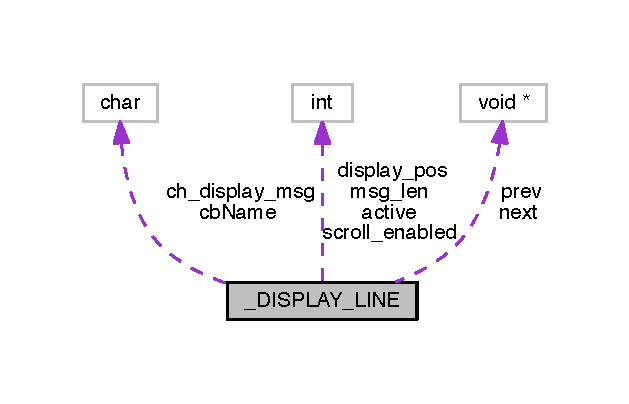
\includegraphics[width=302pt]{struct___d_i_s_p_l_a_y___l_i_n_e__coll__graph}
\end{center}
\end{figure}
\subsection*{Data Fields}
\begin{DoxyCompactItemize}
\item 
char \hyperlink{struct___d_i_s_p_l_a_y___l_i_n_e_a3a374d209578adb1d4cea933756fb14a}{cb\+Name} \mbox{[}\hyperlink{skn__common__headers_8h_a8d2978ad614b0de81c60483e706d9306}{S\+Z\+\_\+\+C\+H\+A\+R\+\_\+\+B\+U\+F\+F}\mbox{]}
\item 
int \hyperlink{struct___d_i_s_p_l_a_y___l_i_n_e_acf235d7965b9d52439add787b8e3d316}{active}
\item 
char \hyperlink{struct___d_i_s_p_l_a_y___l_i_n_e_ae5fae9b599281d1d3f619b6e402e7c2c}{ch\+\_\+display\+\_\+msg} \mbox{[}\hyperlink{skn__common__headers_8h_a442d5e93bd9c9d8eb4532aba62b5f86c}{S\+Z\+\_\+\+I\+N\+F\+O\+\_\+\+B\+U\+F\+F}\mbox{]}
\item 
int \hyperlink{struct___d_i_s_p_l_a_y___l_i_n_e_aa9cfa1dd3e90386f675fef61e711342e}{msg\+\_\+len}
\item 
int \hyperlink{struct___d_i_s_p_l_a_y___l_i_n_e_af32b1aa2ce817c27695d7cd43db9364d}{display\+\_\+pos}
\item 
int \hyperlink{struct___d_i_s_p_l_a_y___l_i_n_e_ad92346a9708f3f3ba0c45dfb891c18e3}{scroll\+\_\+enabled}
\item 
void $\ast$ \hyperlink{struct___d_i_s_p_l_a_y___l_i_n_e_a0668a4de4eb91d9bbd03cc52b00f4fd0}{next}
\item 
void $\ast$ \hyperlink{struct___d_i_s_p_l_a_y___l_i_n_e_aadc57636aadef3cff11443217e7f50e5}{prev}
\end{DoxyCompactItemize}


\subsection{Detailed Description}


Definition at line 287 of file skn\+\_\+common\+\_\+headers.\+h.



\subsection{Field Documentation}
\hypertarget{struct___d_i_s_p_l_a_y___l_i_n_e_acf235d7965b9d52439add787b8e3d316}{}\index{\+\_\+\+D\+I\+S\+P\+L\+A\+Y\+\_\+\+L\+I\+N\+E@{\+\_\+\+D\+I\+S\+P\+L\+A\+Y\+\_\+\+L\+I\+N\+E}!active@{active}}
\index{active@{active}!\+\_\+\+D\+I\+S\+P\+L\+A\+Y\+\_\+\+L\+I\+N\+E@{\+\_\+\+D\+I\+S\+P\+L\+A\+Y\+\_\+\+L\+I\+N\+E}}
\subsubsection[{active}]{\setlength{\rightskip}{0pt plus 5cm}int \+\_\+\+D\+I\+S\+P\+L\+A\+Y\+\_\+\+L\+I\+N\+E\+::active}\label{struct___d_i_s_p_l_a_y___l_i_n_e_acf235d7965b9d52439add787b8e3d316}


Definition at line 289 of file skn\+\_\+common\+\_\+headers.\+h.



Referenced by skn\+\_\+display\+\_\+manager\+\_\+add\+\_\+line(), skn\+\_\+display\+\_\+manager\+\_\+create(), and skn\+\_\+display\+\_\+manager\+\_\+do\+\_\+work().

\hypertarget{struct___d_i_s_p_l_a_y___l_i_n_e_a3a374d209578adb1d4cea933756fb14a}{}\index{\+\_\+\+D\+I\+S\+P\+L\+A\+Y\+\_\+\+L\+I\+N\+E@{\+\_\+\+D\+I\+S\+P\+L\+A\+Y\+\_\+\+L\+I\+N\+E}!cb\+Name@{cb\+Name}}
\index{cb\+Name@{cb\+Name}!\+\_\+\+D\+I\+S\+P\+L\+A\+Y\+\_\+\+L\+I\+N\+E@{\+\_\+\+D\+I\+S\+P\+L\+A\+Y\+\_\+\+L\+I\+N\+E}}
\subsubsection[{cb\+Name}]{\setlength{\rightskip}{0pt plus 5cm}char \+\_\+\+D\+I\+S\+P\+L\+A\+Y\+\_\+\+L\+I\+N\+E\+::cb\+Name\mbox{[}{\bf S\+Z\+\_\+\+C\+H\+A\+R\+\_\+\+B\+U\+F\+F}\mbox{]}}\label{struct___d_i_s_p_l_a_y___l_i_n_e_a3a374d209578adb1d4cea933756fb14a}


Definition at line 288 of file skn\+\_\+common\+\_\+headers.\+h.



Referenced by skn\+\_\+display\+\_\+manager\+\_\+create().

\hypertarget{struct___d_i_s_p_l_a_y___l_i_n_e_ae5fae9b599281d1d3f619b6e402e7c2c}{}\index{\+\_\+\+D\+I\+S\+P\+L\+A\+Y\+\_\+\+L\+I\+N\+E@{\+\_\+\+D\+I\+S\+P\+L\+A\+Y\+\_\+\+L\+I\+N\+E}!ch\+\_\+display\+\_\+msg@{ch\+\_\+display\+\_\+msg}}
\index{ch\+\_\+display\+\_\+msg@{ch\+\_\+display\+\_\+msg}!\+\_\+\+D\+I\+S\+P\+L\+A\+Y\+\_\+\+L\+I\+N\+E@{\+\_\+\+D\+I\+S\+P\+L\+A\+Y\+\_\+\+L\+I\+N\+E}}
\subsubsection[{ch\+\_\+display\+\_\+msg}]{\setlength{\rightskip}{0pt plus 5cm}char \+\_\+\+D\+I\+S\+P\+L\+A\+Y\+\_\+\+L\+I\+N\+E\+::ch\+\_\+display\+\_\+msg\mbox{[}{\bf S\+Z\+\_\+\+I\+N\+F\+O\+\_\+\+B\+U\+F\+F}\mbox{]}}\label{struct___d_i_s_p_l_a_y___l_i_n_e_ae5fae9b599281d1d3f619b6e402e7c2c}


Definition at line 290 of file skn\+\_\+common\+\_\+headers.\+h.



Referenced by skn\+\_\+display\+\_\+manager\+\_\+add\+\_\+line(), skn\+\_\+display\+\_\+manager\+\_\+create(), and skn\+\_\+scroller\+\_\+scroll\+\_\+lines().

\hypertarget{struct___d_i_s_p_l_a_y___l_i_n_e_af32b1aa2ce817c27695d7cd43db9364d}{}\index{\+\_\+\+D\+I\+S\+P\+L\+A\+Y\+\_\+\+L\+I\+N\+E@{\+\_\+\+D\+I\+S\+P\+L\+A\+Y\+\_\+\+L\+I\+N\+E}!display\+\_\+pos@{display\+\_\+pos}}
\index{display\+\_\+pos@{display\+\_\+pos}!\+\_\+\+D\+I\+S\+P\+L\+A\+Y\+\_\+\+L\+I\+N\+E@{\+\_\+\+D\+I\+S\+P\+L\+A\+Y\+\_\+\+L\+I\+N\+E}}
\subsubsection[{display\+\_\+pos}]{\setlength{\rightskip}{0pt plus 5cm}int \+\_\+\+D\+I\+S\+P\+L\+A\+Y\+\_\+\+L\+I\+N\+E\+::display\+\_\+pos}\label{struct___d_i_s_p_l_a_y___l_i_n_e_af32b1aa2ce817c27695d7cd43db9364d}


Definition at line 292 of file skn\+\_\+common\+\_\+headers.\+h.



Referenced by skn\+\_\+display\+\_\+manager\+\_\+add\+\_\+line(), and skn\+\_\+scroller\+\_\+scroll\+\_\+lines().

\hypertarget{struct___d_i_s_p_l_a_y___l_i_n_e_aa9cfa1dd3e90386f675fef61e711342e}{}\index{\+\_\+\+D\+I\+S\+P\+L\+A\+Y\+\_\+\+L\+I\+N\+E@{\+\_\+\+D\+I\+S\+P\+L\+A\+Y\+\_\+\+L\+I\+N\+E}!msg\+\_\+len@{msg\+\_\+len}}
\index{msg\+\_\+len@{msg\+\_\+len}!\+\_\+\+D\+I\+S\+P\+L\+A\+Y\+\_\+\+L\+I\+N\+E@{\+\_\+\+D\+I\+S\+P\+L\+A\+Y\+\_\+\+L\+I\+N\+E}}
\subsubsection[{msg\+\_\+len}]{\setlength{\rightskip}{0pt plus 5cm}int \+\_\+\+D\+I\+S\+P\+L\+A\+Y\+\_\+\+L\+I\+N\+E\+::msg\+\_\+len}\label{struct___d_i_s_p_l_a_y___l_i_n_e_aa9cfa1dd3e90386f675fef61e711342e}


Definition at line 291 of file skn\+\_\+common\+\_\+headers.\+h.



Referenced by skn\+\_\+display\+\_\+manager\+\_\+add\+\_\+line(), skn\+\_\+display\+\_\+manager\+\_\+create(), and skn\+\_\+scroller\+\_\+scroll\+\_\+lines().

\hypertarget{struct___d_i_s_p_l_a_y___l_i_n_e_a0668a4de4eb91d9bbd03cc52b00f4fd0}{}\index{\+\_\+\+D\+I\+S\+P\+L\+A\+Y\+\_\+\+L\+I\+N\+E@{\+\_\+\+D\+I\+S\+P\+L\+A\+Y\+\_\+\+L\+I\+N\+E}!next@{next}}
\index{next@{next}!\+\_\+\+D\+I\+S\+P\+L\+A\+Y\+\_\+\+L\+I\+N\+E@{\+\_\+\+D\+I\+S\+P\+L\+A\+Y\+\_\+\+L\+I\+N\+E}}
\subsubsection[{next}]{\setlength{\rightskip}{0pt plus 5cm}void$\ast$ \+\_\+\+D\+I\+S\+P\+L\+A\+Y\+\_\+\+L\+I\+N\+E\+::next}\label{struct___d_i_s_p_l_a_y___l_i_n_e_a0668a4de4eb91d9bbd03cc52b00f4fd0}


Definition at line 294 of file skn\+\_\+common\+\_\+headers.\+h.



Referenced by skn\+\_\+display\+\_\+manager\+\_\+create(), and skn\+\_\+display\+\_\+manager\+\_\+do\+\_\+work().

\hypertarget{struct___d_i_s_p_l_a_y___l_i_n_e_aadc57636aadef3cff11443217e7f50e5}{}\index{\+\_\+\+D\+I\+S\+P\+L\+A\+Y\+\_\+\+L\+I\+N\+E@{\+\_\+\+D\+I\+S\+P\+L\+A\+Y\+\_\+\+L\+I\+N\+E}!prev@{prev}}
\index{prev@{prev}!\+\_\+\+D\+I\+S\+P\+L\+A\+Y\+\_\+\+L\+I\+N\+E@{\+\_\+\+D\+I\+S\+P\+L\+A\+Y\+\_\+\+L\+I\+N\+E}}
\subsubsection[{prev}]{\setlength{\rightskip}{0pt plus 5cm}void$\ast$ \+\_\+\+D\+I\+S\+P\+L\+A\+Y\+\_\+\+L\+I\+N\+E\+::prev}\label{struct___d_i_s_p_l_a_y___l_i_n_e_aadc57636aadef3cff11443217e7f50e5}


Definition at line 295 of file skn\+\_\+common\+\_\+headers.\+h.



Referenced by skn\+\_\+display\+\_\+manager\+\_\+create().

\hypertarget{struct___d_i_s_p_l_a_y___l_i_n_e_ad92346a9708f3f3ba0c45dfb891c18e3}{}\index{\+\_\+\+D\+I\+S\+P\+L\+A\+Y\+\_\+\+L\+I\+N\+E@{\+\_\+\+D\+I\+S\+P\+L\+A\+Y\+\_\+\+L\+I\+N\+E}!scroll\+\_\+enabled@{scroll\+\_\+enabled}}
\index{scroll\+\_\+enabled@{scroll\+\_\+enabled}!\+\_\+\+D\+I\+S\+P\+L\+A\+Y\+\_\+\+L\+I\+N\+E@{\+\_\+\+D\+I\+S\+P\+L\+A\+Y\+\_\+\+L\+I\+N\+E}}
\subsubsection[{scroll\+\_\+enabled}]{\setlength{\rightskip}{0pt plus 5cm}int \+\_\+\+D\+I\+S\+P\+L\+A\+Y\+\_\+\+L\+I\+N\+E\+::scroll\+\_\+enabled}\label{struct___d_i_s_p_l_a_y___l_i_n_e_ad92346a9708f3f3ba0c45dfb891c18e3}


Definition at line 293 of file skn\+\_\+common\+\_\+headers.\+h.



Referenced by skn\+\_\+display\+\_\+manager\+\_\+add\+\_\+line(), and skn\+\_\+display\+\_\+manager\+\_\+create().



The documentation for this struct was generated from the following file\+:\begin{DoxyCompactItemize}
\item 
src/\hyperlink{skn__common__headers_8h}{skn\+\_\+common\+\_\+headers.\+h}\end{DoxyCompactItemize}

\hypertarget{struct___d_i_s_p_l_a_y___m_a_n_a_g_e_r}{}\section{\+\_\+\+D\+I\+S\+P\+L\+A\+Y\+\_\+\+M\+A\+N\+A\+G\+ER Struct Reference}
\label{struct___d_i_s_p_l_a_y___m_a_n_a_g_e_r}\index{\+\_\+\+D\+I\+S\+P\+L\+A\+Y\+\_\+\+M\+A\+N\+A\+G\+ER@{\+\_\+\+D\+I\+S\+P\+L\+A\+Y\+\_\+\+M\+A\+N\+A\+G\+ER}}


{\ttfamily \#include $<$skn\+\_\+common\+\_\+headers.\+h$>$}



Collaboration diagram for \+\_\+\+D\+I\+S\+P\+L\+A\+Y\+\_\+\+M\+A\+N\+A\+G\+ER\+:\nopagebreak
\begin{figure}[H]
\begin{center}
\leavevmode
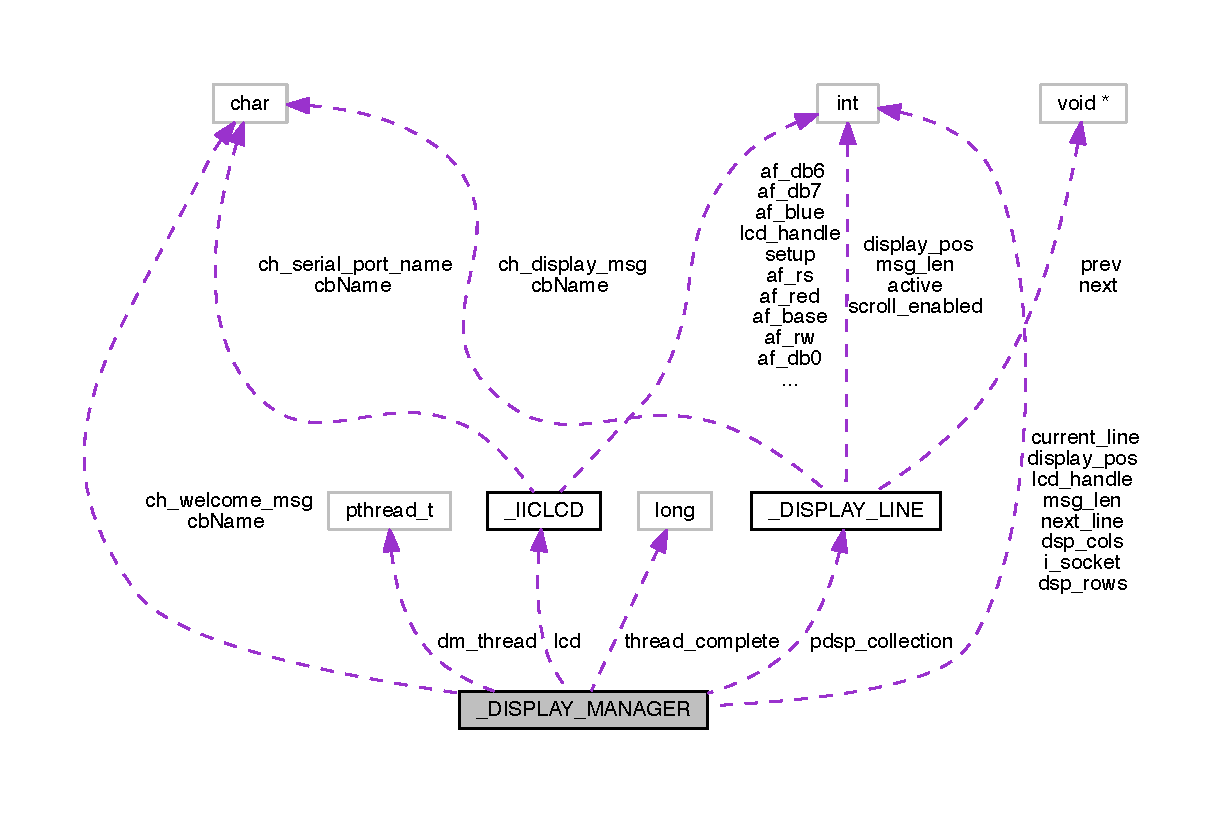
\includegraphics[width=350pt]{struct___d_i_s_p_l_a_y___m_a_n_a_g_e_r__coll__graph}
\end{center}
\end{figure}
\subsection*{Data Fields}
\begin{DoxyCompactItemize}
\item 
char \hyperlink{struct___d_i_s_p_l_a_y___m_a_n_a_g_e_r_abfad08e99f5f76d9e63de7d1fb88befd}{cb\+Name} \mbox{[}\hyperlink{skn__common__headers_8h_a8d2978ad614b0de81c60483e706d9306}{S\+Z\+\_\+\+C\+H\+A\+R\+\_\+\+B\+U\+FF}\mbox{]}
\item 
char \hyperlink{struct___d_i_s_p_l_a_y___m_a_n_a_g_e_r_a4ddfa233f1e3d41609f10b23a386541e}{ch\+\_\+welcome\+\_\+msg} \mbox{[}\hyperlink{skn__common__headers_8h_a442d5e93bd9c9d8eb4532aba62b5f86c}{S\+Z\+\_\+\+I\+N\+F\+O\+\_\+\+B\+U\+FF}\mbox{]}
\item 
int \hyperlink{struct___d_i_s_p_l_a_y___m_a_n_a_g_e_r_a10067d9a5974f5f19bf638ee72ddd973}{msg\+\_\+len}
\item 
int \hyperlink{struct___d_i_s_p_l_a_y___m_a_n_a_g_e_r_aa910f0f6b6ce599a8be02853214d860c}{display\+\_\+pos}
\item 
int \hyperlink{struct___d_i_s_p_l_a_y___m_a_n_a_g_e_r_aeddcffcc90a611efde00a085352bc63b}{dsp\+\_\+rows}
\item 
int \hyperlink{struct___d_i_s_p_l_a_y___m_a_n_a_g_e_r_a8ea0b9503de7da47f210489c8fa19867}{dsp\+\_\+cols}
\item 
\hyperlink{skn__common__headers_8h_a754e9456a497a668b8d959ed2cbe9ec3}{P\+Display\+Line} \hyperlink{struct___d_i_s_p_l_a_y___m_a_n_a_g_e_r_a3a5ccb906320bd6aecbf89cb6b0fc234}{pdsp\+\_\+collection} \mbox{[}\hyperlink{skn__common__headers_8h_a199b80b777af46c9141191749f8f026d}{A\+R\+Y\+\_\+\+M\+A\+X\+\_\+\+D\+M\+\_\+\+L\+I\+N\+ES}\mbox{]}
\item 
int \hyperlink{struct___d_i_s_p_l_a_y___m_a_n_a_g_e_r_aae8a6a90422fd9f571dff5f455740aa4}{current\+\_\+line}
\item 
int \hyperlink{struct___d_i_s_p_l_a_y___m_a_n_a_g_e_r_aed299ac3603bba3dfe3c09389122f8d8}{next\+\_\+line}
\item 
int \hyperlink{struct___d_i_s_p_l_a_y___m_a_n_a_g_e_r_a6ebc44b98c1483295586660829eb5a43}{lcd\+\_\+handle}
\item 
pthread\+\_\+t \hyperlink{struct___d_i_s_p_l_a_y___m_a_n_a_g_e_r_a7033f795cd887063d36c11556c368e6f}{dm\+\_\+thread}
\item 
long \hyperlink{struct___d_i_s_p_l_a_y___m_a_n_a_g_e_r_ae20e9cf0e6789ce07c5b8005b4a7ada0}{thread\+\_\+complete}
\item 
int \hyperlink{struct___d_i_s_p_l_a_y___m_a_n_a_g_e_r_a23e726562acd51d59c09eafa6f179137}{i\+\_\+socket}
\item 
\hyperlink{skn__common__headers_8h_a0f995b3ca5c58b83622b2faea0d21cb8}{L\+C\+D\+Device} \hyperlink{struct___d_i_s_p_l_a_y___m_a_n_a_g_e_r_a182e9fb6ca9f11b3e0a35628123d46f5}{lcd}
\end{DoxyCompactItemize}


\subsection{Detailed Description}


Definition at line 298 of file skn\+\_\+common\+\_\+headers.\+h.



\subsection{Field Documentation}
\index{\+\_\+\+D\+I\+S\+P\+L\+A\+Y\+\_\+\+M\+A\+N\+A\+G\+ER@{\+\_\+\+D\+I\+S\+P\+L\+A\+Y\+\_\+\+M\+A\+N\+A\+G\+ER}!cb\+Name@{cb\+Name}}
\index{cb\+Name@{cb\+Name}!\+\_\+\+D\+I\+S\+P\+L\+A\+Y\+\_\+\+M\+A\+N\+A\+G\+ER@{\+\_\+\+D\+I\+S\+P\+L\+A\+Y\+\_\+\+M\+A\+N\+A\+G\+ER}}
\subsubsection[{\texorpdfstring{cb\+Name}{cbName}}]{\setlength{\rightskip}{0pt plus 5cm}char \+\_\+\+D\+I\+S\+P\+L\+A\+Y\+\_\+\+M\+A\+N\+A\+G\+E\+R\+::cb\+Name\mbox{[}{\bf S\+Z\+\_\+\+C\+H\+A\+R\+\_\+\+B\+U\+FF}\mbox{]}}\hypertarget{struct___d_i_s_p_l_a_y___m_a_n_a_g_e_r_abfad08e99f5f76d9e63de7d1fb88befd}{}\label{struct___d_i_s_p_l_a_y___m_a_n_a_g_e_r_abfad08e99f5f76d9e63de7d1fb88befd}


Definition at line 299 of file skn\+\_\+common\+\_\+headers.\+h.



Referenced by skn\+\_\+display\+\_\+manager\+\_\+create().

\index{\+\_\+\+D\+I\+S\+P\+L\+A\+Y\+\_\+\+M\+A\+N\+A\+G\+ER@{\+\_\+\+D\+I\+S\+P\+L\+A\+Y\+\_\+\+M\+A\+N\+A\+G\+ER}!ch\+\_\+welcome\+\_\+msg@{ch\+\_\+welcome\+\_\+msg}}
\index{ch\+\_\+welcome\+\_\+msg@{ch\+\_\+welcome\+\_\+msg}!\+\_\+\+D\+I\+S\+P\+L\+A\+Y\+\_\+\+M\+A\+N\+A\+G\+ER@{\+\_\+\+D\+I\+S\+P\+L\+A\+Y\+\_\+\+M\+A\+N\+A\+G\+ER}}
\subsubsection[{\texorpdfstring{ch\+\_\+welcome\+\_\+msg}{ch_welcome_msg}}]{\setlength{\rightskip}{0pt plus 5cm}char \+\_\+\+D\+I\+S\+P\+L\+A\+Y\+\_\+\+M\+A\+N\+A\+G\+E\+R\+::ch\+\_\+welcome\+\_\+msg\mbox{[}{\bf S\+Z\+\_\+\+I\+N\+F\+O\+\_\+\+B\+U\+FF}\mbox{]}}\hypertarget{struct___d_i_s_p_l_a_y___m_a_n_a_g_e_r_a4ddfa233f1e3d41609f10b23a386541e}{}\label{struct___d_i_s_p_l_a_y___m_a_n_a_g_e_r_a4ddfa233f1e3d41609f10b23a386541e}


Definition at line 300 of file skn\+\_\+common\+\_\+headers.\+h.



Referenced by skn\+\_\+display\+\_\+manager\+\_\+create().

\index{\+\_\+\+D\+I\+S\+P\+L\+A\+Y\+\_\+\+M\+A\+N\+A\+G\+ER@{\+\_\+\+D\+I\+S\+P\+L\+A\+Y\+\_\+\+M\+A\+N\+A\+G\+ER}!current\+\_\+line@{current\+\_\+line}}
\index{current\+\_\+line@{current\+\_\+line}!\+\_\+\+D\+I\+S\+P\+L\+A\+Y\+\_\+\+M\+A\+N\+A\+G\+ER@{\+\_\+\+D\+I\+S\+P\+L\+A\+Y\+\_\+\+M\+A\+N\+A\+G\+ER}}
\subsubsection[{\texorpdfstring{current\+\_\+line}{current_line}}]{\setlength{\rightskip}{0pt plus 5cm}int \+\_\+\+D\+I\+S\+P\+L\+A\+Y\+\_\+\+M\+A\+N\+A\+G\+E\+R\+::current\+\_\+line}\hypertarget{struct___d_i_s_p_l_a_y___m_a_n_a_g_e_r_aae8a6a90422fd9f571dff5f455740aa4}{}\label{struct___d_i_s_p_l_a_y___m_a_n_a_g_e_r_aae8a6a90422fd9f571dff5f455740aa4}


Definition at line 306 of file skn\+\_\+common\+\_\+headers.\+h.



Referenced by skn\+\_\+display\+\_\+manager\+\_\+add\+\_\+line(), skn\+\_\+display\+\_\+manager\+\_\+create(), and skn\+\_\+display\+\_\+manager\+\_\+do\+\_\+work().

\index{\+\_\+\+D\+I\+S\+P\+L\+A\+Y\+\_\+\+M\+A\+N\+A\+G\+ER@{\+\_\+\+D\+I\+S\+P\+L\+A\+Y\+\_\+\+M\+A\+N\+A\+G\+ER}!display\+\_\+pos@{display\+\_\+pos}}
\index{display\+\_\+pos@{display\+\_\+pos}!\+\_\+\+D\+I\+S\+P\+L\+A\+Y\+\_\+\+M\+A\+N\+A\+G\+ER@{\+\_\+\+D\+I\+S\+P\+L\+A\+Y\+\_\+\+M\+A\+N\+A\+G\+ER}}
\subsubsection[{\texorpdfstring{display\+\_\+pos}{display_pos}}]{\setlength{\rightskip}{0pt plus 5cm}int \+\_\+\+D\+I\+S\+P\+L\+A\+Y\+\_\+\+M\+A\+N\+A\+G\+E\+R\+::display\+\_\+pos}\hypertarget{struct___d_i_s_p_l_a_y___m_a_n_a_g_e_r_aa910f0f6b6ce599a8be02853214d860c}{}\label{struct___d_i_s_p_l_a_y___m_a_n_a_g_e_r_aa910f0f6b6ce599a8be02853214d860c}


Definition at line 302 of file skn\+\_\+common\+\_\+headers.\+h.

\index{\+\_\+\+D\+I\+S\+P\+L\+A\+Y\+\_\+\+M\+A\+N\+A\+G\+ER@{\+\_\+\+D\+I\+S\+P\+L\+A\+Y\+\_\+\+M\+A\+N\+A\+G\+ER}!dm\+\_\+thread@{dm\+\_\+thread}}
\index{dm\+\_\+thread@{dm\+\_\+thread}!\+\_\+\+D\+I\+S\+P\+L\+A\+Y\+\_\+\+M\+A\+N\+A\+G\+ER@{\+\_\+\+D\+I\+S\+P\+L\+A\+Y\+\_\+\+M\+A\+N\+A\+G\+ER}}
\subsubsection[{\texorpdfstring{dm\+\_\+thread}{dm_thread}}]{\setlength{\rightskip}{0pt plus 5cm}pthread\+\_\+t \+\_\+\+D\+I\+S\+P\+L\+A\+Y\+\_\+\+M\+A\+N\+A\+G\+E\+R\+::dm\+\_\+thread}\hypertarget{struct___d_i_s_p_l_a_y___m_a_n_a_g_e_r_a7033f795cd887063d36c11556c368e6f}{}\label{struct___d_i_s_p_l_a_y___m_a_n_a_g_e_r_a7033f795cd887063d36c11556c368e6f}


Definition at line 309 of file skn\+\_\+common\+\_\+headers.\+h.



Referenced by skn\+\_\+display\+\_\+manager\+\_\+message\+\_\+consumer\+\_\+shutdown(), and skn\+\_\+display\+\_\+manager\+\_\+message\+\_\+consumer\+\_\+startup().

\index{\+\_\+\+D\+I\+S\+P\+L\+A\+Y\+\_\+\+M\+A\+N\+A\+G\+ER@{\+\_\+\+D\+I\+S\+P\+L\+A\+Y\+\_\+\+M\+A\+N\+A\+G\+ER}!dsp\+\_\+cols@{dsp\+\_\+cols}}
\index{dsp\+\_\+cols@{dsp\+\_\+cols}!\+\_\+\+D\+I\+S\+P\+L\+A\+Y\+\_\+\+M\+A\+N\+A\+G\+ER@{\+\_\+\+D\+I\+S\+P\+L\+A\+Y\+\_\+\+M\+A\+N\+A\+G\+ER}}
\subsubsection[{\texorpdfstring{dsp\+\_\+cols}{dsp_cols}}]{\setlength{\rightskip}{0pt plus 5cm}int \+\_\+\+D\+I\+S\+P\+L\+A\+Y\+\_\+\+M\+A\+N\+A\+G\+E\+R\+::dsp\+\_\+cols}\hypertarget{struct___d_i_s_p_l_a_y___m_a_n_a_g_e_r_a8ea0b9503de7da47f210489c8fa19867}{}\label{struct___d_i_s_p_l_a_y___m_a_n_a_g_e_r_a8ea0b9503de7da47f210489c8fa19867}


Definition at line 304 of file skn\+\_\+common\+\_\+headers.\+h.



Referenced by skn\+\_\+device\+\_\+manager\+\_\+init\+\_\+i2c(), and skn\+\_\+display\+\_\+manager\+\_\+create().

\index{\+\_\+\+D\+I\+S\+P\+L\+A\+Y\+\_\+\+M\+A\+N\+A\+G\+ER@{\+\_\+\+D\+I\+S\+P\+L\+A\+Y\+\_\+\+M\+A\+N\+A\+G\+ER}!dsp\+\_\+rows@{dsp\+\_\+rows}}
\index{dsp\+\_\+rows@{dsp\+\_\+rows}!\+\_\+\+D\+I\+S\+P\+L\+A\+Y\+\_\+\+M\+A\+N\+A\+G\+ER@{\+\_\+\+D\+I\+S\+P\+L\+A\+Y\+\_\+\+M\+A\+N\+A\+G\+ER}}
\subsubsection[{\texorpdfstring{dsp\+\_\+rows}{dsp_rows}}]{\setlength{\rightskip}{0pt plus 5cm}int \+\_\+\+D\+I\+S\+P\+L\+A\+Y\+\_\+\+M\+A\+N\+A\+G\+E\+R\+::dsp\+\_\+rows}\hypertarget{struct___d_i_s_p_l_a_y___m_a_n_a_g_e_r_aeddcffcc90a611efde00a085352bc63b}{}\label{struct___d_i_s_p_l_a_y___m_a_n_a_g_e_r_aeddcffcc90a611efde00a085352bc63b}


Definition at line 303 of file skn\+\_\+common\+\_\+headers.\+h.



Referenced by skn\+\_\+device\+\_\+manager\+\_\+init\+\_\+i2c(), skn\+\_\+display\+\_\+manager\+\_\+create(), and skn\+\_\+display\+\_\+manager\+\_\+do\+\_\+work().

\index{\+\_\+\+D\+I\+S\+P\+L\+A\+Y\+\_\+\+M\+A\+N\+A\+G\+ER@{\+\_\+\+D\+I\+S\+P\+L\+A\+Y\+\_\+\+M\+A\+N\+A\+G\+ER}!i\+\_\+socket@{i\+\_\+socket}}
\index{i\+\_\+socket@{i\+\_\+socket}!\+\_\+\+D\+I\+S\+P\+L\+A\+Y\+\_\+\+M\+A\+N\+A\+G\+ER@{\+\_\+\+D\+I\+S\+P\+L\+A\+Y\+\_\+\+M\+A\+N\+A\+G\+ER}}
\subsubsection[{\texorpdfstring{i\+\_\+socket}{i_socket}}]{\setlength{\rightskip}{0pt plus 5cm}int \+\_\+\+D\+I\+S\+P\+L\+A\+Y\+\_\+\+M\+A\+N\+A\+G\+E\+R\+::i\+\_\+socket}\hypertarget{struct___d_i_s_p_l_a_y___m_a_n_a_g_e_r_a23e726562acd51d59c09eafa6f179137}{}\label{struct___d_i_s_p_l_a_y___m_a_n_a_g_e_r_a23e726562acd51d59c09eafa6f179137}


Definition at line 311 of file skn\+\_\+common\+\_\+headers.\+h.



Referenced by skn\+\_\+display\+\_\+manager\+\_\+message\+\_\+consumer\+\_\+shutdown(), skn\+\_\+display\+\_\+manager\+\_\+message\+\_\+consumer\+\_\+startup(), and skn\+\_\+display\+\_\+manager\+\_\+message\+\_\+consumer\+\_\+thread().

\index{\+\_\+\+D\+I\+S\+P\+L\+A\+Y\+\_\+\+M\+A\+N\+A\+G\+ER@{\+\_\+\+D\+I\+S\+P\+L\+A\+Y\+\_\+\+M\+A\+N\+A\+G\+ER}!lcd@{lcd}}
\index{lcd@{lcd}!\+\_\+\+D\+I\+S\+P\+L\+A\+Y\+\_\+\+M\+A\+N\+A\+G\+ER@{\+\_\+\+D\+I\+S\+P\+L\+A\+Y\+\_\+\+M\+A\+N\+A\+G\+ER}}
\subsubsection[{\texorpdfstring{lcd}{lcd}}]{\setlength{\rightskip}{0pt plus 5cm}{\bf L\+C\+D\+Device} \+\_\+\+D\+I\+S\+P\+L\+A\+Y\+\_\+\+M\+A\+N\+A\+G\+E\+R\+::lcd}\hypertarget{struct___d_i_s_p_l_a_y___m_a_n_a_g_e_r_a182e9fb6ca9f11b3e0a35628123d46f5}{}\label{struct___d_i_s_p_l_a_y___m_a_n_a_g_e_r_a182e9fb6ca9f11b3e0a35628123d46f5}


Definition at line 312 of file skn\+\_\+common\+\_\+headers.\+h.



Referenced by skn\+\_\+device\+\_\+manager\+\_\+init\+\_\+i2c(), skn\+\_\+device\+\_\+manager\+\_\+\+L\+C\+D\+\_\+shutdown(), skn\+\_\+device\+\_\+manager\+\_\+\+M\+C\+P23008(), skn\+\_\+device\+\_\+manager\+\_\+\+M\+C\+P23017(), skn\+\_\+device\+\_\+manager\+\_\+\+P\+C\+F8574(), and skn\+\_\+device\+\_\+manager\+\_\+\+Serial\+Port().

\index{\+\_\+\+D\+I\+S\+P\+L\+A\+Y\+\_\+\+M\+A\+N\+A\+G\+ER@{\+\_\+\+D\+I\+S\+P\+L\+A\+Y\+\_\+\+M\+A\+N\+A\+G\+ER}!lcd\+\_\+handle@{lcd\+\_\+handle}}
\index{lcd\+\_\+handle@{lcd\+\_\+handle}!\+\_\+\+D\+I\+S\+P\+L\+A\+Y\+\_\+\+M\+A\+N\+A\+G\+ER@{\+\_\+\+D\+I\+S\+P\+L\+A\+Y\+\_\+\+M\+A\+N\+A\+G\+ER}}
\subsubsection[{\texorpdfstring{lcd\+\_\+handle}{lcd_handle}}]{\setlength{\rightskip}{0pt plus 5cm}int \+\_\+\+D\+I\+S\+P\+L\+A\+Y\+\_\+\+M\+A\+N\+A\+G\+E\+R\+::lcd\+\_\+handle}\hypertarget{struct___d_i_s_p_l_a_y___m_a_n_a_g_e_r_a6ebc44b98c1483295586660829eb5a43}{}\label{struct___d_i_s_p_l_a_y___m_a_n_a_g_e_r_a6ebc44b98c1483295586660829eb5a43}


Definition at line 308 of file skn\+\_\+common\+\_\+headers.\+h.



Referenced by skn\+\_\+device\+\_\+manager\+\_\+init\+\_\+i2c(), skn\+\_\+device\+\_\+manager\+\_\+\+L\+C\+D\+\_\+setup(), skn\+\_\+device\+\_\+manager\+\_\+\+L\+C\+D\+\_\+shutdown(), skn\+\_\+device\+\_\+manager\+\_\+\+Serial\+Port(), and skn\+\_\+display\+\_\+manager\+\_\+do\+\_\+work().

\index{\+\_\+\+D\+I\+S\+P\+L\+A\+Y\+\_\+\+M\+A\+N\+A\+G\+ER@{\+\_\+\+D\+I\+S\+P\+L\+A\+Y\+\_\+\+M\+A\+N\+A\+G\+ER}!msg\+\_\+len@{msg\+\_\+len}}
\index{msg\+\_\+len@{msg\+\_\+len}!\+\_\+\+D\+I\+S\+P\+L\+A\+Y\+\_\+\+M\+A\+N\+A\+G\+ER@{\+\_\+\+D\+I\+S\+P\+L\+A\+Y\+\_\+\+M\+A\+N\+A\+G\+ER}}
\subsubsection[{\texorpdfstring{msg\+\_\+len}{msg_len}}]{\setlength{\rightskip}{0pt plus 5cm}int \+\_\+\+D\+I\+S\+P\+L\+A\+Y\+\_\+\+M\+A\+N\+A\+G\+E\+R\+::msg\+\_\+len}\hypertarget{struct___d_i_s_p_l_a_y___m_a_n_a_g_e_r_a10067d9a5974f5f19bf638ee72ddd973}{}\label{struct___d_i_s_p_l_a_y___m_a_n_a_g_e_r_a10067d9a5974f5f19bf638ee72ddd973}


Definition at line 301 of file skn\+\_\+common\+\_\+headers.\+h.



Referenced by skn\+\_\+display\+\_\+manager\+\_\+create().

\index{\+\_\+\+D\+I\+S\+P\+L\+A\+Y\+\_\+\+M\+A\+N\+A\+G\+ER@{\+\_\+\+D\+I\+S\+P\+L\+A\+Y\+\_\+\+M\+A\+N\+A\+G\+ER}!next\+\_\+line@{next\+\_\+line}}
\index{next\+\_\+line@{next\+\_\+line}!\+\_\+\+D\+I\+S\+P\+L\+A\+Y\+\_\+\+M\+A\+N\+A\+G\+ER@{\+\_\+\+D\+I\+S\+P\+L\+A\+Y\+\_\+\+M\+A\+N\+A\+G\+ER}}
\subsubsection[{\texorpdfstring{next\+\_\+line}{next_line}}]{\setlength{\rightskip}{0pt plus 5cm}int \+\_\+\+D\+I\+S\+P\+L\+A\+Y\+\_\+\+M\+A\+N\+A\+G\+E\+R\+::next\+\_\+line}\hypertarget{struct___d_i_s_p_l_a_y___m_a_n_a_g_e_r_aed299ac3603bba3dfe3c09389122f8d8}{}\label{struct___d_i_s_p_l_a_y___m_a_n_a_g_e_r_aed299ac3603bba3dfe3c09389122f8d8}


Definition at line 307 of file skn\+\_\+common\+\_\+headers.\+h.



Referenced by skn\+\_\+display\+\_\+manager\+\_\+add\+\_\+line(), and skn\+\_\+display\+\_\+manager\+\_\+create().

\index{\+\_\+\+D\+I\+S\+P\+L\+A\+Y\+\_\+\+M\+A\+N\+A\+G\+ER@{\+\_\+\+D\+I\+S\+P\+L\+A\+Y\+\_\+\+M\+A\+N\+A\+G\+ER}!pdsp\+\_\+collection@{pdsp\+\_\+collection}}
\index{pdsp\+\_\+collection@{pdsp\+\_\+collection}!\+\_\+\+D\+I\+S\+P\+L\+A\+Y\+\_\+\+M\+A\+N\+A\+G\+ER@{\+\_\+\+D\+I\+S\+P\+L\+A\+Y\+\_\+\+M\+A\+N\+A\+G\+ER}}
\subsubsection[{\texorpdfstring{pdsp\+\_\+collection}{pdsp_collection}}]{\setlength{\rightskip}{0pt plus 5cm}{\bf P\+Display\+Line} \+\_\+\+D\+I\+S\+P\+L\+A\+Y\+\_\+\+M\+A\+N\+A\+G\+E\+R\+::pdsp\+\_\+collection\mbox{[}{\bf A\+R\+Y\+\_\+\+M\+A\+X\+\_\+\+D\+M\+\_\+\+L\+I\+N\+ES}\mbox{]}}\hypertarget{struct___d_i_s_p_l_a_y___m_a_n_a_g_e_r_a3a5ccb906320bd6aecbf89cb6b0fc234}{}\label{struct___d_i_s_p_l_a_y___m_a_n_a_g_e_r_a3a5ccb906320bd6aecbf89cb6b0fc234}


Definition at line 305 of file skn\+\_\+common\+\_\+headers.\+h.



Referenced by skn\+\_\+display\+\_\+manager\+\_\+add\+\_\+line(), skn\+\_\+display\+\_\+manager\+\_\+create(), skn\+\_\+display\+\_\+manager\+\_\+destroy(), and skn\+\_\+display\+\_\+manager\+\_\+do\+\_\+work().

\index{\+\_\+\+D\+I\+S\+P\+L\+A\+Y\+\_\+\+M\+A\+N\+A\+G\+ER@{\+\_\+\+D\+I\+S\+P\+L\+A\+Y\+\_\+\+M\+A\+N\+A\+G\+ER}!thread\+\_\+complete@{thread\+\_\+complete}}
\index{thread\+\_\+complete@{thread\+\_\+complete}!\+\_\+\+D\+I\+S\+P\+L\+A\+Y\+\_\+\+M\+A\+N\+A\+G\+ER@{\+\_\+\+D\+I\+S\+P\+L\+A\+Y\+\_\+\+M\+A\+N\+A\+G\+ER}}
\subsubsection[{\texorpdfstring{thread\+\_\+complete}{thread_complete}}]{\setlength{\rightskip}{0pt plus 5cm}long \+\_\+\+D\+I\+S\+P\+L\+A\+Y\+\_\+\+M\+A\+N\+A\+G\+E\+R\+::thread\+\_\+complete}\hypertarget{struct___d_i_s_p_l_a_y___m_a_n_a_g_e_r_ae20e9cf0e6789ce07c5b8005b4a7ada0}{}\label{struct___d_i_s_p_l_a_y___m_a_n_a_g_e_r_ae20e9cf0e6789ce07c5b8005b4a7ada0}


Definition at line 310 of file skn\+\_\+common\+\_\+headers.\+h.



Referenced by skn\+\_\+display\+\_\+manager\+\_\+message\+\_\+consumer\+\_\+shutdown(), and skn\+\_\+display\+\_\+manager\+\_\+message\+\_\+consumer\+\_\+thread().



The documentation for this struct was generated from the following file\+:\begin{DoxyCompactItemize}
\item 
src/\hyperlink{skn__common__headers_8h}{skn\+\_\+common\+\_\+headers.\+h}\end{DoxyCompactItemize}

\hypertarget{struct__gssdp_registry_data}{\section{\+\_\+gssdp\+Registry\+Data Struct Reference}
\label{struct__gssdp_registry_data}\index{\+\_\+gssdp\+Registry\+Data@{\+\_\+gssdp\+Registry\+Data}}
}


Collaboration diagram for \+\_\+gssdp\+Registry\+Data\+:\nopagebreak
\begin{figure}[H]
\begin{center}
\leavevmode
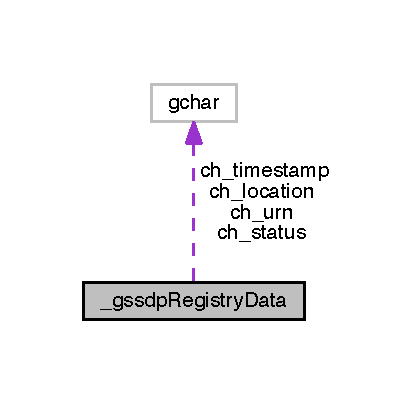
\includegraphics[width=198pt]{struct__gssdp_registry_data__coll__graph}
\end{center}
\end{figure}
\subsection*{Data Fields}
\begin{DoxyCompactItemize}
\item 
gchar \hyperlink{struct__gssdp_registry_data_a97c1fccf55465d4de2168be0d70e2707}{ch\+\_\+timestamp} \mbox{[}\hyperlink{gtk_d_s_8c_ac08ad1b127f1c9743c5592ffb796423f}{S\+Z\+\_\+\+T\+I\+M\+E\+S\+T\+A\+M\+P\+\_\+\+B\+U\+F\+F}\mbox{]}
\item 
gchar \hyperlink{struct__gssdp_registry_data_a57a14b78092cbef8cf6dfa56cffa03db}{ch\+\_\+urn} \mbox{[}\hyperlink{gtk_d_s_8c_a152ca8fa1a2eac39d1badafb6c6cef8c}{S\+Z\+\_\+\+R\+M\+T\+A\+D\+D\+R\+\_\+\+B\+U\+F\+F}\mbox{]}
\item 
gchar \hyperlink{struct__gssdp_registry_data_ac1ca256d22c387e9ef968fb8413d7796}{ch\+\_\+location} \mbox{[}\hyperlink{gtk_d_s_8c_a152ca8fa1a2eac39d1badafb6c6cef8c}{S\+Z\+\_\+\+R\+M\+T\+A\+D\+D\+R\+\_\+\+B\+U\+F\+F}\mbox{]}
\item 
gchar \hyperlink{struct__gssdp_registry_data_a92d851353d8779ad1c5dd4e540a956e5}{ch\+\_\+status} \mbox{[}\hyperlink{gtk_d_s_8c_ac21e8a77d073e7a5383c92bb485992c8}{S\+Z\+\_\+\+P\+A\+R\+A\+M\+S\+\_\+\+B\+U\+F\+F}\mbox{]}
\end{DoxyCompactItemize}


\subsection{Detailed Description}


Definition at line 91 of file gssdp\+D\+C.\+c.



\subsection{Field Documentation}
\hypertarget{struct__gssdp_registry_data_ac1ca256d22c387e9ef968fb8413d7796}{\index{\+\_\+gssdp\+Registry\+Data@{\+\_\+gssdp\+Registry\+Data}!ch\+\_\+location@{ch\+\_\+location}}
\index{ch\+\_\+location@{ch\+\_\+location}!\+\_\+gssdp\+Registry\+Data@{\+\_\+gssdp\+Registry\+Data}}
\subsubsection[{ch\+\_\+location}]{\setlength{\rightskip}{0pt plus 5cm}gchar \+\_\+gssdp\+Registry\+Data\+::ch\+\_\+location}}\label{struct__gssdp_registry_data_ac1ca256d22c387e9ef968fb8413d7796}


Definition at line 94 of file gssdp\+D\+C.\+c.



Referenced by cb\+\_\+gssdp\+\_\+resource\+\_\+available(), cb\+\_\+gssdp\+\_\+resource\+\_\+unavailable(), cb\+\_\+udp\+\_\+registry\+\_\+select\+\_\+handler(), and ui\+\_\+add\+\_\+gssdp\+\_\+registry\+\_\+entry().

\hypertarget{struct__gssdp_registry_data_a92d851353d8779ad1c5dd4e540a956e5}{\index{\+\_\+gssdp\+Registry\+Data@{\+\_\+gssdp\+Registry\+Data}!ch\+\_\+status@{ch\+\_\+status}}
\index{ch\+\_\+status@{ch\+\_\+status}!\+\_\+gssdp\+Registry\+Data@{\+\_\+gssdp\+Registry\+Data}}
\subsubsection[{ch\+\_\+status}]{\setlength{\rightskip}{0pt plus 5cm}gchar \+\_\+gssdp\+Registry\+Data\+::ch\+\_\+status}}\label{struct__gssdp_registry_data_a92d851353d8779ad1c5dd4e540a956e5}


Definition at line 95 of file gssdp\+D\+C.\+c.



Referenced by cb\+\_\+gssdp\+\_\+resource\+\_\+available(), cb\+\_\+gssdp\+\_\+resource\+\_\+unavailable(), and ui\+\_\+add\+\_\+gssdp\+\_\+registry\+\_\+entry().

\hypertarget{struct__gssdp_registry_data_a97c1fccf55465d4de2168be0d70e2707}{\index{\+\_\+gssdp\+Registry\+Data@{\+\_\+gssdp\+Registry\+Data}!ch\+\_\+timestamp@{ch\+\_\+timestamp}}
\index{ch\+\_\+timestamp@{ch\+\_\+timestamp}!\+\_\+gssdp\+Registry\+Data@{\+\_\+gssdp\+Registry\+Data}}
\subsubsection[{ch\+\_\+timestamp}]{\setlength{\rightskip}{0pt plus 5cm}gchar \+\_\+gssdp\+Registry\+Data\+::ch\+\_\+timestamp}}\label{struct__gssdp_registry_data_a97c1fccf55465d4de2168be0d70e2707}


Definition at line 92 of file gssdp\+D\+C.\+c.



Referenced by cb\+\_\+gssdp\+\_\+resource\+\_\+available(), cb\+\_\+gssdp\+\_\+resource\+\_\+unavailable(), and ui\+\_\+add\+\_\+gssdp\+\_\+registry\+\_\+entry().

\hypertarget{struct__gssdp_registry_data_a57a14b78092cbef8cf6dfa56cffa03db}{\index{\+\_\+gssdp\+Registry\+Data@{\+\_\+gssdp\+Registry\+Data}!ch\+\_\+urn@{ch\+\_\+urn}}
\index{ch\+\_\+urn@{ch\+\_\+urn}!\+\_\+gssdp\+Registry\+Data@{\+\_\+gssdp\+Registry\+Data}}
\subsubsection[{ch\+\_\+urn}]{\setlength{\rightskip}{0pt plus 5cm}gchar \+\_\+gssdp\+Registry\+Data\+::ch\+\_\+urn}}\label{struct__gssdp_registry_data_a57a14b78092cbef8cf6dfa56cffa03db}


Definition at line 93 of file gssdp\+D\+C.\+c.



Referenced by cb\+\_\+gssdp\+\_\+resource\+\_\+available(), cb\+\_\+gssdp\+\_\+resource\+\_\+unavailable(), cb\+\_\+udp\+\_\+registry\+\_\+select\+\_\+handler(), udp\+\_\+registry\+\_\+find\+\_\+by\+\_\+name(), and ui\+\_\+add\+\_\+gssdp\+\_\+registry\+\_\+entry().



The documentation for this struct was generated from the following files\+:\begin{DoxyCompactItemize}
\item 
gssdp\+D\+C/\hyperlink{gssdp_d_c_8c}{gssdp\+D\+C.\+c}\item 
gtk\+D\+S/\hyperlink{gtk_d_s_8c}{gtk\+D\+S.\+c}\end{DoxyCompactItemize}

\hypertarget{struct___i_i_c_l_c_d}{}\section{\+\_\+\+I\+I\+C\+L\+CD Struct Reference}
\label{struct___i_i_c_l_c_d}\index{\+\_\+\+I\+I\+C\+L\+CD@{\+\_\+\+I\+I\+C\+L\+CD}}


{\ttfamily \#include $<$skn\+\_\+common\+\_\+headers.\+h$>$}



Collaboration diagram for \+\_\+\+I\+I\+C\+L\+CD\+:\nopagebreak
\begin{figure}[H]
\begin{center}
\leavevmode
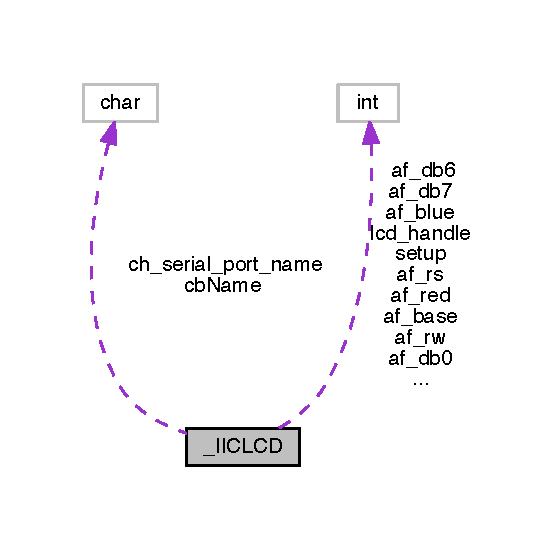
\includegraphics[width=266pt]{struct___i_i_c_l_c_d__coll__graph}
\end{center}
\end{figure}
\subsection*{Data Fields}
\begin{DoxyCompactItemize}
\item 
char \hyperlink{struct___i_i_c_l_c_d_a3f9347595482a6da5cb5d536d937a554}{cb\+Name} \mbox{[}\hyperlink{skn__common__headers_8h_a8d2978ad614b0de81c60483e706d9306}{S\+Z\+\_\+\+C\+H\+A\+R\+\_\+\+B\+U\+FF}\mbox{]}
\item 
char \hyperlink{struct___i_i_c_l_c_d_a2f193b0806fdbba1d644567835e2b2e8}{ch\+\_\+serial\+\_\+port\+\_\+name} \mbox{[}\hyperlink{skn__common__headers_8h_a8d2978ad614b0de81c60483e706d9306}{S\+Z\+\_\+\+C\+H\+A\+R\+\_\+\+B\+U\+FF}\mbox{]}
\item 
int \hyperlink{struct___i_i_c_l_c_d_afc74b2d9120be4a8e69e48b220d6781c}{lcd\+\_\+handle}
\item 
int \hyperlink{struct___i_i_c_l_c_d_a3f3fe8757875939b987ac0c416081551}{i2c\+\_\+address}
\item 
int \hyperlink{struct___i_i_c_l_c_d_ae74954b1b96523d617a68e42c2663086}{af\+\_\+base}
\item 
int \hyperlink{struct___i_i_c_l_c_d_ad160086a31276fbaf849855519b9878e}{af\+\_\+backlight}
\item 
int \hyperlink{struct___i_i_c_l_c_d_aca8ab39cfa9f683b2d03269886a0f633}{af\+\_\+red}
\item 
int \hyperlink{struct___i_i_c_l_c_d_a70176d63c9065d4186f55ae8328a82d3}{af\+\_\+green}
\item 
int \hyperlink{struct___i_i_c_l_c_d_ad64bc4c5fc6a592f161e594f0b2433e1}{af\+\_\+blue}
\item 
int \hyperlink{struct___i_i_c_l_c_d_a896f8305b5c0395ea7f9074904047b32}{af\+\_\+e}
\item 
int \hyperlink{struct___i_i_c_l_c_d_af738bf1e020daaa5476b917c375e807a}{af\+\_\+rs}
\item 
int \hyperlink{struct___i_i_c_l_c_d_ad0162f6a3e82c34192c0d901ef0ff6be}{af\+\_\+rw}
\item 
int \hyperlink{struct___i_i_c_l_c_d_a86dfd51ffdc849569bc91bba9f9cd4a6}{af\+\_\+db0}
\item 
int \hyperlink{struct___i_i_c_l_c_d_a114a5f81c889fe857d714a3a5033b397}{af\+\_\+db1}
\item 
int \hyperlink{struct___i_i_c_l_c_d_a7b88e6903c8fb93882c396261ffe40b5}{af\+\_\+db2}
\item 
int \hyperlink{struct___i_i_c_l_c_d_a26f362cb78eb2227a14706e9c992a066}{af\+\_\+db3}
\item 
int \hyperlink{struct___i_i_c_l_c_d_adbfc88b661d5da527aad6f5bcd45a85c}{af\+\_\+db4}
\item 
int \hyperlink{struct___i_i_c_l_c_d_a41c4536106493476b52c9a9df9dd8599}{af\+\_\+db5}
\item 
int \hyperlink{struct___i_i_c_l_c_d_a0f3ebbe756ecf62494733287f64821f9}{af\+\_\+db6}
\item 
int \hyperlink{struct___i_i_c_l_c_d_ae55385ca612fd157fb85e7b3d5423ee4}{af\+\_\+db7}
\item 
int($\ast$ \hyperlink{struct___i_i_c_l_c_d_ab3052517b34cbf67239b91ccbd113c00}{setup} )(const int, const int)
\end{DoxyCompactItemize}


\subsection{Detailed Description}


Definition at line 216 of file skn\+\_\+common\+\_\+headers.\+h.



\subsection{Field Documentation}
\index{\+\_\+\+I\+I\+C\+L\+CD@{\+\_\+\+I\+I\+C\+L\+CD}!af\+\_\+backlight@{af\+\_\+backlight}}
\index{af\+\_\+backlight@{af\+\_\+backlight}!\+\_\+\+I\+I\+C\+L\+CD@{\+\_\+\+I\+I\+C\+L\+CD}}
\subsubsection[{\texorpdfstring{af\+\_\+backlight}{af_backlight}}]{\setlength{\rightskip}{0pt plus 5cm}int \+\_\+\+I\+I\+C\+L\+C\+D\+::af\+\_\+backlight}\hypertarget{struct___i_i_c_l_c_d_ad160086a31276fbaf849855519b9878e}{}\label{struct___i_i_c_l_c_d_ad160086a31276fbaf849855519b9878e}


Definition at line 222 of file skn\+\_\+common\+\_\+headers.\+h.



Referenced by skn\+\_\+device\+\_\+manager\+\_\+init\+\_\+i2c(), skn\+\_\+device\+\_\+manager\+\_\+\+L\+C\+D\+\_\+shutdown(), skn\+\_\+device\+\_\+manager\+\_\+\+M\+C\+P23008(), skn\+\_\+device\+\_\+manager\+\_\+\+M\+C\+P23017(), and skn\+\_\+device\+\_\+manager\+\_\+\+P\+C\+F8574().

\index{\+\_\+\+I\+I\+C\+L\+CD@{\+\_\+\+I\+I\+C\+L\+CD}!af\+\_\+base@{af\+\_\+base}}
\index{af\+\_\+base@{af\+\_\+base}!\+\_\+\+I\+I\+C\+L\+CD@{\+\_\+\+I\+I\+C\+L\+CD}}
\subsubsection[{\texorpdfstring{af\+\_\+base}{af_base}}]{\setlength{\rightskip}{0pt plus 5cm}int \+\_\+\+I\+I\+C\+L\+C\+D\+::af\+\_\+base}\hypertarget{struct___i_i_c_l_c_d_ae74954b1b96523d617a68e42c2663086}{}\label{struct___i_i_c_l_c_d_ae74954b1b96523d617a68e42c2663086}


Definition at line 221 of file skn\+\_\+common\+\_\+headers.\+h.



Referenced by skn\+\_\+device\+\_\+manager\+\_\+init\+\_\+i2c(), skn\+\_\+device\+\_\+manager\+\_\+\+M\+C\+P23008(), skn\+\_\+device\+\_\+manager\+\_\+\+M\+C\+P23017(), and skn\+\_\+device\+\_\+manager\+\_\+\+P\+C\+F8574().

\index{\+\_\+\+I\+I\+C\+L\+CD@{\+\_\+\+I\+I\+C\+L\+CD}!af\+\_\+blue@{af\+\_\+blue}}
\index{af\+\_\+blue@{af\+\_\+blue}!\+\_\+\+I\+I\+C\+L\+CD@{\+\_\+\+I\+I\+C\+L\+CD}}
\subsubsection[{\texorpdfstring{af\+\_\+blue}{af_blue}}]{\setlength{\rightskip}{0pt plus 5cm}int \+\_\+\+I\+I\+C\+L\+C\+D\+::af\+\_\+blue}\hypertarget{struct___i_i_c_l_c_d_ad64bc4c5fc6a592f161e594f0b2433e1}{}\label{struct___i_i_c_l_c_d_ad64bc4c5fc6a592f161e594f0b2433e1}


Definition at line 225 of file skn\+\_\+common\+\_\+headers.\+h.



Referenced by skn\+\_\+device\+\_\+manager\+\_\+init\+\_\+i2c(), skn\+\_\+device\+\_\+manager\+\_\+\+L\+C\+D\+\_\+shutdown(), and skn\+\_\+device\+\_\+manager\+\_\+\+M\+C\+P23017().

\index{\+\_\+\+I\+I\+C\+L\+CD@{\+\_\+\+I\+I\+C\+L\+CD}!af\+\_\+db0@{af\+\_\+db0}}
\index{af\+\_\+db0@{af\+\_\+db0}!\+\_\+\+I\+I\+C\+L\+CD@{\+\_\+\+I\+I\+C\+L\+CD}}
\subsubsection[{\texorpdfstring{af\+\_\+db0}{af_db0}}]{\setlength{\rightskip}{0pt plus 5cm}int \+\_\+\+I\+I\+C\+L\+C\+D\+::af\+\_\+db0}\hypertarget{struct___i_i_c_l_c_d_a86dfd51ffdc849569bc91bba9f9cd4a6}{}\label{struct___i_i_c_l_c_d_a86dfd51ffdc849569bc91bba9f9cd4a6}


Definition at line 231 of file skn\+\_\+common\+\_\+headers.\+h.



Referenced by skn\+\_\+device\+\_\+manager\+\_\+init\+\_\+i2c().

\index{\+\_\+\+I\+I\+C\+L\+CD@{\+\_\+\+I\+I\+C\+L\+CD}!af\+\_\+db1@{af\+\_\+db1}}
\index{af\+\_\+db1@{af\+\_\+db1}!\+\_\+\+I\+I\+C\+L\+CD@{\+\_\+\+I\+I\+C\+L\+CD}}
\subsubsection[{\texorpdfstring{af\+\_\+db1}{af_db1}}]{\setlength{\rightskip}{0pt plus 5cm}int \+\_\+\+I\+I\+C\+L\+C\+D\+::af\+\_\+db1}\hypertarget{struct___i_i_c_l_c_d_a114a5f81c889fe857d714a3a5033b397}{}\label{struct___i_i_c_l_c_d_a114a5f81c889fe857d714a3a5033b397}


Definition at line 232 of file skn\+\_\+common\+\_\+headers.\+h.



Referenced by skn\+\_\+device\+\_\+manager\+\_\+init\+\_\+i2c().

\index{\+\_\+\+I\+I\+C\+L\+CD@{\+\_\+\+I\+I\+C\+L\+CD}!af\+\_\+db2@{af\+\_\+db2}}
\index{af\+\_\+db2@{af\+\_\+db2}!\+\_\+\+I\+I\+C\+L\+CD@{\+\_\+\+I\+I\+C\+L\+CD}}
\subsubsection[{\texorpdfstring{af\+\_\+db2}{af_db2}}]{\setlength{\rightskip}{0pt plus 5cm}int \+\_\+\+I\+I\+C\+L\+C\+D\+::af\+\_\+db2}\hypertarget{struct___i_i_c_l_c_d_a7b88e6903c8fb93882c396261ffe40b5}{}\label{struct___i_i_c_l_c_d_a7b88e6903c8fb93882c396261ffe40b5}


Definition at line 233 of file skn\+\_\+common\+\_\+headers.\+h.



Referenced by skn\+\_\+device\+\_\+manager\+\_\+init\+\_\+i2c().

\index{\+\_\+\+I\+I\+C\+L\+CD@{\+\_\+\+I\+I\+C\+L\+CD}!af\+\_\+db3@{af\+\_\+db3}}
\index{af\+\_\+db3@{af\+\_\+db3}!\+\_\+\+I\+I\+C\+L\+CD@{\+\_\+\+I\+I\+C\+L\+CD}}
\subsubsection[{\texorpdfstring{af\+\_\+db3}{af_db3}}]{\setlength{\rightskip}{0pt plus 5cm}int \+\_\+\+I\+I\+C\+L\+C\+D\+::af\+\_\+db3}\hypertarget{struct___i_i_c_l_c_d_a26f362cb78eb2227a14706e9c992a066}{}\label{struct___i_i_c_l_c_d_a26f362cb78eb2227a14706e9c992a066}


Definition at line 234 of file skn\+\_\+common\+\_\+headers.\+h.



Referenced by skn\+\_\+device\+\_\+manager\+\_\+init\+\_\+i2c().

\index{\+\_\+\+I\+I\+C\+L\+CD@{\+\_\+\+I\+I\+C\+L\+CD}!af\+\_\+db4@{af\+\_\+db4}}
\index{af\+\_\+db4@{af\+\_\+db4}!\+\_\+\+I\+I\+C\+L\+CD@{\+\_\+\+I\+I\+C\+L\+CD}}
\subsubsection[{\texorpdfstring{af\+\_\+db4}{af_db4}}]{\setlength{\rightskip}{0pt plus 5cm}int \+\_\+\+I\+I\+C\+L\+C\+D\+::af\+\_\+db4}\hypertarget{struct___i_i_c_l_c_d_adbfc88b661d5da527aad6f5bcd45a85c}{}\label{struct___i_i_c_l_c_d_adbfc88b661d5da527aad6f5bcd45a85c}


Definition at line 235 of file skn\+\_\+common\+\_\+headers.\+h.



Referenced by skn\+\_\+device\+\_\+manager\+\_\+init\+\_\+i2c(), skn\+\_\+device\+\_\+manager\+\_\+\+M\+C\+P23008(), skn\+\_\+device\+\_\+manager\+\_\+\+M\+C\+P23017(), and skn\+\_\+device\+\_\+manager\+\_\+\+P\+C\+F8574().

\index{\+\_\+\+I\+I\+C\+L\+CD@{\+\_\+\+I\+I\+C\+L\+CD}!af\+\_\+db5@{af\+\_\+db5}}
\index{af\+\_\+db5@{af\+\_\+db5}!\+\_\+\+I\+I\+C\+L\+CD@{\+\_\+\+I\+I\+C\+L\+CD}}
\subsubsection[{\texorpdfstring{af\+\_\+db5}{af_db5}}]{\setlength{\rightskip}{0pt plus 5cm}int \+\_\+\+I\+I\+C\+L\+C\+D\+::af\+\_\+db5}\hypertarget{struct___i_i_c_l_c_d_a41c4536106493476b52c9a9df9dd8599}{}\label{struct___i_i_c_l_c_d_a41c4536106493476b52c9a9df9dd8599}


Definition at line 236 of file skn\+\_\+common\+\_\+headers.\+h.



Referenced by skn\+\_\+device\+\_\+manager\+\_\+init\+\_\+i2c(), skn\+\_\+device\+\_\+manager\+\_\+\+M\+C\+P23008(), skn\+\_\+device\+\_\+manager\+\_\+\+M\+C\+P23017(), and skn\+\_\+device\+\_\+manager\+\_\+\+P\+C\+F8574().

\index{\+\_\+\+I\+I\+C\+L\+CD@{\+\_\+\+I\+I\+C\+L\+CD}!af\+\_\+db6@{af\+\_\+db6}}
\index{af\+\_\+db6@{af\+\_\+db6}!\+\_\+\+I\+I\+C\+L\+CD@{\+\_\+\+I\+I\+C\+L\+CD}}
\subsubsection[{\texorpdfstring{af\+\_\+db6}{af_db6}}]{\setlength{\rightskip}{0pt plus 5cm}int \+\_\+\+I\+I\+C\+L\+C\+D\+::af\+\_\+db6}\hypertarget{struct___i_i_c_l_c_d_a0f3ebbe756ecf62494733287f64821f9}{}\label{struct___i_i_c_l_c_d_a0f3ebbe756ecf62494733287f64821f9}


Definition at line 237 of file skn\+\_\+common\+\_\+headers.\+h.



Referenced by skn\+\_\+device\+\_\+manager\+\_\+init\+\_\+i2c(), skn\+\_\+device\+\_\+manager\+\_\+\+M\+C\+P23008(), skn\+\_\+device\+\_\+manager\+\_\+\+M\+C\+P23017(), and skn\+\_\+device\+\_\+manager\+\_\+\+P\+C\+F8574().

\index{\+\_\+\+I\+I\+C\+L\+CD@{\+\_\+\+I\+I\+C\+L\+CD}!af\+\_\+db7@{af\+\_\+db7}}
\index{af\+\_\+db7@{af\+\_\+db7}!\+\_\+\+I\+I\+C\+L\+CD@{\+\_\+\+I\+I\+C\+L\+CD}}
\subsubsection[{\texorpdfstring{af\+\_\+db7}{af_db7}}]{\setlength{\rightskip}{0pt plus 5cm}int \+\_\+\+I\+I\+C\+L\+C\+D\+::af\+\_\+db7}\hypertarget{struct___i_i_c_l_c_d_ae55385ca612fd157fb85e7b3d5423ee4}{}\label{struct___i_i_c_l_c_d_ae55385ca612fd157fb85e7b3d5423ee4}


Definition at line 238 of file skn\+\_\+common\+\_\+headers.\+h.



Referenced by skn\+\_\+device\+\_\+manager\+\_\+init\+\_\+i2c(), skn\+\_\+device\+\_\+manager\+\_\+\+M\+C\+P23008(), skn\+\_\+device\+\_\+manager\+\_\+\+M\+C\+P23017(), and skn\+\_\+device\+\_\+manager\+\_\+\+P\+C\+F8574().

\index{\+\_\+\+I\+I\+C\+L\+CD@{\+\_\+\+I\+I\+C\+L\+CD}!af\+\_\+e@{af\+\_\+e}}
\index{af\+\_\+e@{af\+\_\+e}!\+\_\+\+I\+I\+C\+L\+CD@{\+\_\+\+I\+I\+C\+L\+CD}}
\subsubsection[{\texorpdfstring{af\+\_\+e}{af_e}}]{\setlength{\rightskip}{0pt plus 5cm}int \+\_\+\+I\+I\+C\+L\+C\+D\+::af\+\_\+e}\hypertarget{struct___i_i_c_l_c_d_a896f8305b5c0395ea7f9074904047b32}{}\label{struct___i_i_c_l_c_d_a896f8305b5c0395ea7f9074904047b32}


Definition at line 227 of file skn\+\_\+common\+\_\+headers.\+h.



Referenced by skn\+\_\+device\+\_\+manager\+\_\+init\+\_\+i2c(), skn\+\_\+device\+\_\+manager\+\_\+\+M\+C\+P23008(), skn\+\_\+device\+\_\+manager\+\_\+\+M\+C\+P23017(), and skn\+\_\+device\+\_\+manager\+\_\+\+P\+C\+F8574().

\index{\+\_\+\+I\+I\+C\+L\+CD@{\+\_\+\+I\+I\+C\+L\+CD}!af\+\_\+green@{af\+\_\+green}}
\index{af\+\_\+green@{af\+\_\+green}!\+\_\+\+I\+I\+C\+L\+CD@{\+\_\+\+I\+I\+C\+L\+CD}}
\subsubsection[{\texorpdfstring{af\+\_\+green}{af_green}}]{\setlength{\rightskip}{0pt plus 5cm}int \+\_\+\+I\+I\+C\+L\+C\+D\+::af\+\_\+green}\hypertarget{struct___i_i_c_l_c_d_a70176d63c9065d4186f55ae8328a82d3}{}\label{struct___i_i_c_l_c_d_a70176d63c9065d4186f55ae8328a82d3}


Definition at line 224 of file skn\+\_\+common\+\_\+headers.\+h.



Referenced by skn\+\_\+device\+\_\+manager\+\_\+init\+\_\+i2c(), skn\+\_\+device\+\_\+manager\+\_\+\+L\+C\+D\+\_\+shutdown(), and skn\+\_\+device\+\_\+manager\+\_\+\+M\+C\+P23017().

\index{\+\_\+\+I\+I\+C\+L\+CD@{\+\_\+\+I\+I\+C\+L\+CD}!af\+\_\+red@{af\+\_\+red}}
\index{af\+\_\+red@{af\+\_\+red}!\+\_\+\+I\+I\+C\+L\+CD@{\+\_\+\+I\+I\+C\+L\+CD}}
\subsubsection[{\texorpdfstring{af\+\_\+red}{af_red}}]{\setlength{\rightskip}{0pt plus 5cm}int \+\_\+\+I\+I\+C\+L\+C\+D\+::af\+\_\+red}\hypertarget{struct___i_i_c_l_c_d_aca8ab39cfa9f683b2d03269886a0f633}{}\label{struct___i_i_c_l_c_d_aca8ab39cfa9f683b2d03269886a0f633}


Definition at line 223 of file skn\+\_\+common\+\_\+headers.\+h.



Referenced by skn\+\_\+device\+\_\+manager\+\_\+init\+\_\+i2c(), skn\+\_\+device\+\_\+manager\+\_\+\+L\+C\+D\+\_\+shutdown(), and skn\+\_\+device\+\_\+manager\+\_\+\+M\+C\+P23017().

\index{\+\_\+\+I\+I\+C\+L\+CD@{\+\_\+\+I\+I\+C\+L\+CD}!af\+\_\+rs@{af\+\_\+rs}}
\index{af\+\_\+rs@{af\+\_\+rs}!\+\_\+\+I\+I\+C\+L\+CD@{\+\_\+\+I\+I\+C\+L\+CD}}
\subsubsection[{\texorpdfstring{af\+\_\+rs}{af_rs}}]{\setlength{\rightskip}{0pt plus 5cm}int \+\_\+\+I\+I\+C\+L\+C\+D\+::af\+\_\+rs}\hypertarget{struct___i_i_c_l_c_d_af738bf1e020daaa5476b917c375e807a}{}\label{struct___i_i_c_l_c_d_af738bf1e020daaa5476b917c375e807a}


Definition at line 228 of file skn\+\_\+common\+\_\+headers.\+h.



Referenced by skn\+\_\+device\+\_\+manager\+\_\+init\+\_\+i2c(), skn\+\_\+device\+\_\+manager\+\_\+\+M\+C\+P23008(), skn\+\_\+device\+\_\+manager\+\_\+\+M\+C\+P23017(), and skn\+\_\+device\+\_\+manager\+\_\+\+P\+C\+F8574().

\index{\+\_\+\+I\+I\+C\+L\+CD@{\+\_\+\+I\+I\+C\+L\+CD}!af\+\_\+rw@{af\+\_\+rw}}
\index{af\+\_\+rw@{af\+\_\+rw}!\+\_\+\+I\+I\+C\+L\+CD@{\+\_\+\+I\+I\+C\+L\+CD}}
\subsubsection[{\texorpdfstring{af\+\_\+rw}{af_rw}}]{\setlength{\rightskip}{0pt plus 5cm}int \+\_\+\+I\+I\+C\+L\+C\+D\+::af\+\_\+rw}\hypertarget{struct___i_i_c_l_c_d_ad0162f6a3e82c34192c0d901ef0ff6be}{}\label{struct___i_i_c_l_c_d_ad0162f6a3e82c34192c0d901ef0ff6be}


Definition at line 229 of file skn\+\_\+common\+\_\+headers.\+h.



Referenced by skn\+\_\+device\+\_\+manager\+\_\+init\+\_\+i2c(), skn\+\_\+device\+\_\+manager\+\_\+\+M\+C\+P23008(), skn\+\_\+device\+\_\+manager\+\_\+\+M\+C\+P23017(), and skn\+\_\+device\+\_\+manager\+\_\+\+P\+C\+F8574().

\index{\+\_\+\+I\+I\+C\+L\+CD@{\+\_\+\+I\+I\+C\+L\+CD}!cb\+Name@{cb\+Name}}
\index{cb\+Name@{cb\+Name}!\+\_\+\+I\+I\+C\+L\+CD@{\+\_\+\+I\+I\+C\+L\+CD}}
\subsubsection[{\texorpdfstring{cb\+Name}{cbName}}]{\setlength{\rightskip}{0pt plus 5cm}char \+\_\+\+I\+I\+C\+L\+C\+D\+::cb\+Name\mbox{[}{\bf S\+Z\+\_\+\+C\+H\+A\+R\+\_\+\+B\+U\+FF}\mbox{]}}\hypertarget{struct___i_i_c_l_c_d_a3f9347595482a6da5cb5d536d937a554}{}\label{struct___i_i_c_l_c_d_a3f9347595482a6da5cb5d536d937a554}


Definition at line 217 of file skn\+\_\+common\+\_\+headers.\+h.



Referenced by skn\+\_\+device\+\_\+manager\+\_\+\+M\+C\+P23008(), skn\+\_\+device\+\_\+manager\+\_\+\+M\+C\+P23017(), skn\+\_\+device\+\_\+manager\+\_\+\+P\+C\+F8574(), and skn\+\_\+device\+\_\+manager\+\_\+\+Serial\+Port().

\index{\+\_\+\+I\+I\+C\+L\+CD@{\+\_\+\+I\+I\+C\+L\+CD}!ch\+\_\+serial\+\_\+port\+\_\+name@{ch\+\_\+serial\+\_\+port\+\_\+name}}
\index{ch\+\_\+serial\+\_\+port\+\_\+name@{ch\+\_\+serial\+\_\+port\+\_\+name}!\+\_\+\+I\+I\+C\+L\+CD@{\+\_\+\+I\+I\+C\+L\+CD}}
\subsubsection[{\texorpdfstring{ch\+\_\+serial\+\_\+port\+\_\+name}{ch_serial_port_name}}]{\setlength{\rightskip}{0pt plus 5cm}char \+\_\+\+I\+I\+C\+L\+C\+D\+::ch\+\_\+serial\+\_\+port\+\_\+name\mbox{[}{\bf S\+Z\+\_\+\+C\+H\+A\+R\+\_\+\+B\+U\+FF}\mbox{]}}\hypertarget{struct___i_i_c_l_c_d_a2f193b0806fdbba1d644567835e2b2e8}{}\label{struct___i_i_c_l_c_d_a2f193b0806fdbba1d644567835e2b2e8}


Definition at line 218 of file skn\+\_\+common\+\_\+headers.\+h.



Referenced by skn\+\_\+device\+\_\+manager\+\_\+\+Serial\+Port().

\index{\+\_\+\+I\+I\+C\+L\+CD@{\+\_\+\+I\+I\+C\+L\+CD}!i2c\+\_\+address@{i2c\+\_\+address}}
\index{i2c\+\_\+address@{i2c\+\_\+address}!\+\_\+\+I\+I\+C\+L\+CD@{\+\_\+\+I\+I\+C\+L\+CD}}
\subsubsection[{\texorpdfstring{i2c\+\_\+address}{i2c_address}}]{\setlength{\rightskip}{0pt plus 5cm}int \+\_\+\+I\+I\+C\+L\+C\+D\+::i2c\+\_\+address}\hypertarget{struct___i_i_c_l_c_d_a3f3fe8757875939b987ac0c416081551}{}\label{struct___i_i_c_l_c_d_a3f3fe8757875939b987ac0c416081551}


Definition at line 220 of file skn\+\_\+common\+\_\+headers.\+h.



Referenced by skn\+\_\+device\+\_\+manager\+\_\+init\+\_\+i2c(), skn\+\_\+device\+\_\+manager\+\_\+\+M\+C\+P23008(), skn\+\_\+device\+\_\+manager\+\_\+\+M\+C\+P23017(), and skn\+\_\+device\+\_\+manager\+\_\+\+P\+C\+F8574().

\index{\+\_\+\+I\+I\+C\+L\+CD@{\+\_\+\+I\+I\+C\+L\+CD}!lcd\+\_\+handle@{lcd\+\_\+handle}}
\index{lcd\+\_\+handle@{lcd\+\_\+handle}!\+\_\+\+I\+I\+C\+L\+CD@{\+\_\+\+I\+I\+C\+L\+CD}}
\subsubsection[{\texorpdfstring{lcd\+\_\+handle}{lcd_handle}}]{\setlength{\rightskip}{0pt plus 5cm}int \+\_\+\+I\+I\+C\+L\+C\+D\+::lcd\+\_\+handle}\hypertarget{struct___i_i_c_l_c_d_afc74b2d9120be4a8e69e48b220d6781c}{}\label{struct___i_i_c_l_c_d_afc74b2d9120be4a8e69e48b220d6781c}


Definition at line 219 of file skn\+\_\+common\+\_\+headers.\+h.



Referenced by skn\+\_\+device\+\_\+manager\+\_\+init\+\_\+i2c(), and skn\+\_\+device\+\_\+manager\+\_\+\+Serial\+Port().

\index{\+\_\+\+I\+I\+C\+L\+CD@{\+\_\+\+I\+I\+C\+L\+CD}!setup@{setup}}
\index{setup@{setup}!\+\_\+\+I\+I\+C\+L\+CD@{\+\_\+\+I\+I\+C\+L\+CD}}
\subsubsection[{\texorpdfstring{setup}{setup}}]{\setlength{\rightskip}{0pt plus 5cm}int($\ast$ \+\_\+\+I\+I\+C\+L\+C\+D\+::setup) (const int, const int)}\hypertarget{struct___i_i_c_l_c_d_ab3052517b34cbf67239b91ccbd113c00}{}\label{struct___i_i_c_l_c_d_ab3052517b34cbf67239b91ccbd113c00}


Definition at line 239 of file skn\+\_\+common\+\_\+headers.\+h.



Referenced by skn\+\_\+device\+\_\+manager\+\_\+init\+\_\+i2c(), skn\+\_\+device\+\_\+manager\+\_\+\+M\+C\+P23008(), skn\+\_\+device\+\_\+manager\+\_\+\+M\+C\+P23017(), and skn\+\_\+device\+\_\+manager\+\_\+\+P\+C\+F8574().



The documentation for this struct was generated from the following file\+:\begin{DoxyCompactItemize}
\item 
src/\hyperlink{skn__common__headers_8h}{skn\+\_\+common\+\_\+headers.\+h}\end{DoxyCompactItemize}

\hypertarget{struct__ip_broadcast_array}{\section{\+\_\+ip\+Broadcast\+Array Struct Reference}
\label{struct__ip_broadcast_array}\index{\+\_\+ip\+Broadcast\+Array@{\+\_\+ip\+Broadcast\+Array}}
}


{\ttfamily \#include $<$skn\+\_\+common\+\_\+headers.\+h$>$}



Collaboration diagram for \+\_\+ip\+Broadcast\+Array\+:\nopagebreak
\begin{figure}[H]
\begin{center}
\leavevmode
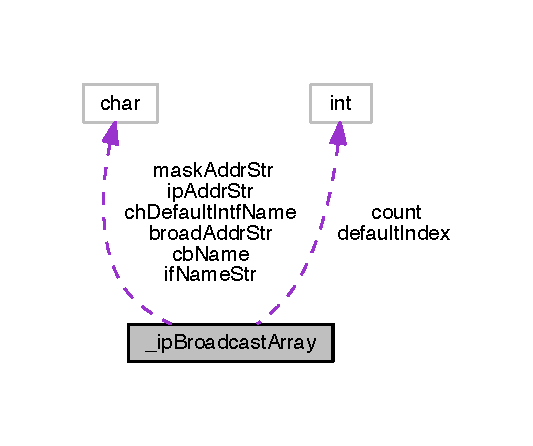
\includegraphics[width=256pt]{struct__ip_broadcast_array__coll__graph}
\end{center}
\end{figure}
\subsection*{Data Fields}
\begin{DoxyCompactItemize}
\item 
char \hyperlink{struct__ip_broadcast_array_a0f592bd31dcc3ce00a349f04ff6bd1ba}{cb\+Name} \mbox{[}\hyperlink{skn__common__headers_8h_a8d2978ad614b0de81c60483e706d9306}{S\+Z\+\_\+\+C\+H\+A\+R\+\_\+\+B\+U\+F\+F}\mbox{]}
\item 
char \hyperlink{struct__ip_broadcast_array_a06dab8742df19b5aec8538842617778d}{ch\+Default\+Intf\+Name} \mbox{[}\hyperlink{skn__common__headers_8h_a8d2978ad614b0de81c60483e706d9306}{S\+Z\+\_\+\+C\+H\+A\+R\+\_\+\+B\+U\+F\+F}\mbox{]}
\item 
char \hyperlink{struct__ip_broadcast_array_a193b90f271c061e8bf1593bab6a182c9}{if\+Name\+Str} \mbox{[}\hyperlink{skn__common__headers_8h_a00b19837422a3b13d82b9a525e92ef51}{A\+R\+Y\+\_\+\+M\+A\+X\+\_\+\+I\+N\+T\+F}\mbox{]}\mbox{[}\hyperlink{skn__common__headers_8h_a8d2978ad614b0de81c60483e706d9306}{S\+Z\+\_\+\+C\+H\+A\+R\+\_\+\+B\+U\+F\+F}\mbox{]}
\item 
char \hyperlink{struct__ip_broadcast_array_a96891ccc707337890b2a166e3ef3a8e1}{ip\+Addr\+Str} \mbox{[}\hyperlink{skn__common__headers_8h_a00b19837422a3b13d82b9a525e92ef51}{A\+R\+Y\+\_\+\+M\+A\+X\+\_\+\+I\+N\+T\+F}\mbox{]}\mbox{[}\hyperlink{skn__common__headers_8h_a8d2978ad614b0de81c60483e706d9306}{S\+Z\+\_\+\+C\+H\+A\+R\+\_\+\+B\+U\+F\+F}\mbox{]}
\item 
char \hyperlink{struct__ip_broadcast_array_a9241c1fbfb22a3ecfe4777863a063eb3}{mask\+Addr\+Str} \mbox{[}\hyperlink{skn__common__headers_8h_a00b19837422a3b13d82b9a525e92ef51}{A\+R\+Y\+\_\+\+M\+A\+X\+\_\+\+I\+N\+T\+F}\mbox{]}\mbox{[}\hyperlink{skn__common__headers_8h_a8d2978ad614b0de81c60483e706d9306}{S\+Z\+\_\+\+C\+H\+A\+R\+\_\+\+B\+U\+F\+F}\mbox{]}
\item 
char \hyperlink{struct__ip_broadcast_array_af40943e174ba847fa0218cfa6051e277}{broad\+Addr\+Str} \mbox{[}\hyperlink{skn__common__headers_8h_a00b19837422a3b13d82b9a525e92ef51}{A\+R\+Y\+\_\+\+M\+A\+X\+\_\+\+I\+N\+T\+F}\mbox{]}\mbox{[}\hyperlink{skn__common__headers_8h_a8d2978ad614b0de81c60483e706d9306}{S\+Z\+\_\+\+C\+H\+A\+R\+\_\+\+B\+U\+F\+F}\mbox{]}
\item 
int \hyperlink{struct__ip_broadcast_array_a5822ff77ae9f31bd3b4298d463c02f1f}{default\+Index}
\item 
int \hyperlink{struct__ip_broadcast_array_a971377a4c995292b8bd908f185cfc844}{count}
\end{DoxyCompactItemize}


\subsection{Detailed Description}


Definition at line 65 of file cmd\+D\+C.\+c.



\subsection{Field Documentation}
\hypertarget{struct__ip_broadcast_array_af40943e174ba847fa0218cfa6051e277}{\index{\+\_\+ip\+Broadcast\+Array@{\+\_\+ip\+Broadcast\+Array}!broad\+Addr\+Str@{broad\+Addr\+Str}}
\index{broad\+Addr\+Str@{broad\+Addr\+Str}!\+\_\+ip\+Broadcast\+Array@{\+\_\+ip\+Broadcast\+Array}}
\subsubsection[{broad\+Addr\+Str}]{\setlength{\rightskip}{0pt plus 5cm}char \+\_\+ip\+Broadcast\+Array\+::broad\+Addr\+Str}}\label{struct__ip_broadcast_array_af40943e174ba847fa0218cfa6051e277}


Definition at line 71 of file cmd\+D\+C.\+c.



Referenced by skn\+\_\+get\+\_\+broadcast\+\_\+ip\+\_\+array(), skn\+\_\+service\+\_\+registry\+\_\+get\+\_\+via\+\_\+udp\+\_\+broadcast(), and skn\+\_\+udp\+\_\+network\+\_\+broadcast\+\_\+all\+\_\+interfaces().

\hypertarget{struct__ip_broadcast_array_a0f592bd31dcc3ce00a349f04ff6bd1ba}{\index{\+\_\+ip\+Broadcast\+Array@{\+\_\+ip\+Broadcast\+Array}!cb\+Name@{cb\+Name}}
\index{cb\+Name@{cb\+Name}!\+\_\+ip\+Broadcast\+Array@{\+\_\+ip\+Broadcast\+Array}}
\subsubsection[{cb\+Name}]{\setlength{\rightskip}{0pt plus 5cm}char \+\_\+ip\+Broadcast\+Array\+::cb\+Name}}\label{struct__ip_broadcast_array_a0f592bd31dcc3ce00a349f04ff6bd1ba}


Definition at line 66 of file cmd\+D\+C.\+c.



Referenced by skn\+\_\+get\+\_\+broadcast\+\_\+ip\+\_\+array().

\hypertarget{struct__ip_broadcast_array_a06dab8742df19b5aec8538842617778d}{\index{\+\_\+ip\+Broadcast\+Array@{\+\_\+ip\+Broadcast\+Array}!ch\+Default\+Intf\+Name@{ch\+Default\+Intf\+Name}}
\index{ch\+Default\+Intf\+Name@{ch\+Default\+Intf\+Name}!\+\_\+ip\+Broadcast\+Array@{\+\_\+ip\+Broadcast\+Array}}
\subsubsection[{ch\+Default\+Intf\+Name}]{\setlength{\rightskip}{0pt plus 5cm}char \+\_\+ip\+Broadcast\+Array\+::ch\+Default\+Intf\+Name}}\label{struct__ip_broadcast_array_a06dab8742df19b5aec8538842617778d}


Definition at line 67 of file cmd\+D\+C.\+c.



Referenced by skn\+\_\+get\+\_\+broadcast\+\_\+ip\+\_\+array(), skn\+\_\+get\+\_\+default\+\_\+interface\+\_\+name\+\_\+and\+\_\+ipv4\+\_\+address(), skn\+\_\+service\+\_\+registry\+\_\+get\+\_\+via\+\_\+udp\+\_\+broadcast(), and skn\+\_\+service\+\_\+registry\+\_\+provider().

\hypertarget{struct__ip_broadcast_array_a971377a4c995292b8bd908f185cfc844}{\index{\+\_\+ip\+Broadcast\+Array@{\+\_\+ip\+Broadcast\+Array}!count@{count}}
\index{count@{count}!\+\_\+ip\+Broadcast\+Array@{\+\_\+ip\+Broadcast\+Array}}
\subsubsection[{count}]{\setlength{\rightskip}{0pt plus 5cm}int \+\_\+ip\+Broadcast\+Array\+::count}}\label{struct__ip_broadcast_array_a971377a4c995292b8bd908f185cfc844}


Definition at line 73 of file cmd\+D\+C.\+c.



Referenced by skn\+\_\+get\+\_\+broadcast\+\_\+ip\+\_\+array(), skn\+\_\+service\+\_\+registry\+\_\+get\+\_\+via\+\_\+udp\+\_\+broadcast(), and skn\+\_\+udp\+\_\+network\+\_\+broadcast\+\_\+all\+\_\+interfaces().

\hypertarget{struct__ip_broadcast_array_a5822ff77ae9f31bd3b4298d463c02f1f}{\index{\+\_\+ip\+Broadcast\+Array@{\+\_\+ip\+Broadcast\+Array}!default\+Index@{default\+Index}}
\index{default\+Index@{default\+Index}!\+\_\+ip\+Broadcast\+Array@{\+\_\+ip\+Broadcast\+Array}}
\subsubsection[{default\+Index}]{\setlength{\rightskip}{0pt plus 5cm}int \+\_\+ip\+Broadcast\+Array\+::default\+Index}}\label{struct__ip_broadcast_array_a5822ff77ae9f31bd3b4298d463c02f1f}


Definition at line 72 of file cmd\+D\+C.\+c.



Referenced by skn\+\_\+get\+\_\+broadcast\+\_\+ip\+\_\+array(), skn\+\_\+get\+\_\+default\+\_\+interface\+\_\+name\+\_\+and\+\_\+ipv4\+\_\+address(), skn\+\_\+service\+\_\+registry\+\_\+get\+\_\+via\+\_\+udp\+\_\+broadcast(), skn\+\_\+service\+\_\+registry\+\_\+provider(), and skn\+\_\+udp\+\_\+network\+\_\+broadcast\+\_\+all\+\_\+interfaces().

\hypertarget{struct__ip_broadcast_array_a193b90f271c061e8bf1593bab6a182c9}{\index{\+\_\+ip\+Broadcast\+Array@{\+\_\+ip\+Broadcast\+Array}!if\+Name\+Str@{if\+Name\+Str}}
\index{if\+Name\+Str@{if\+Name\+Str}!\+\_\+ip\+Broadcast\+Array@{\+\_\+ip\+Broadcast\+Array}}
\subsubsection[{if\+Name\+Str}]{\setlength{\rightskip}{0pt plus 5cm}char \+\_\+ip\+Broadcast\+Array\+::if\+Name\+Str}}\label{struct__ip_broadcast_array_a193b90f271c061e8bf1593bab6a182c9}


Definition at line 68 of file cmd\+D\+C.\+c.



Referenced by skn\+\_\+get\+\_\+broadcast\+\_\+ip\+\_\+array(), skn\+\_\+service\+\_\+registry\+\_\+get\+\_\+via\+\_\+udp\+\_\+broadcast(), and skn\+\_\+udp\+\_\+network\+\_\+broadcast\+\_\+all\+\_\+interfaces().

\hypertarget{struct__ip_broadcast_array_a96891ccc707337890b2a166e3ef3a8e1}{\index{\+\_\+ip\+Broadcast\+Array@{\+\_\+ip\+Broadcast\+Array}!ip\+Addr\+Str@{ip\+Addr\+Str}}
\index{ip\+Addr\+Str@{ip\+Addr\+Str}!\+\_\+ip\+Broadcast\+Array@{\+\_\+ip\+Broadcast\+Array}}
\subsubsection[{ip\+Addr\+Str}]{\setlength{\rightskip}{0pt plus 5cm}char \+\_\+ip\+Broadcast\+Array\+::ip\+Addr\+Str}}\label{struct__ip_broadcast_array_a96891ccc707337890b2a166e3ef3a8e1}


Definition at line 69 of file cmd\+D\+C.\+c.



Referenced by skn\+\_\+get\+\_\+broadcast\+\_\+ip\+\_\+array(), skn\+\_\+get\+\_\+default\+\_\+interface\+\_\+name\+\_\+and\+\_\+ipv4\+\_\+address(), skn\+\_\+service\+\_\+registry\+\_\+get\+\_\+via\+\_\+udp\+\_\+broadcast(), skn\+\_\+service\+\_\+registry\+\_\+provider(), and skn\+\_\+udp\+\_\+network\+\_\+broadcast\+\_\+all\+\_\+interfaces().

\hypertarget{struct__ip_broadcast_array_a9241c1fbfb22a3ecfe4777863a063eb3}{\index{\+\_\+ip\+Broadcast\+Array@{\+\_\+ip\+Broadcast\+Array}!mask\+Addr\+Str@{mask\+Addr\+Str}}
\index{mask\+Addr\+Str@{mask\+Addr\+Str}!\+\_\+ip\+Broadcast\+Array@{\+\_\+ip\+Broadcast\+Array}}
\subsubsection[{mask\+Addr\+Str}]{\setlength{\rightskip}{0pt plus 5cm}char \+\_\+ip\+Broadcast\+Array\+::mask\+Addr\+Str}}\label{struct__ip_broadcast_array_a9241c1fbfb22a3ecfe4777863a063eb3}


Definition at line 70 of file cmd\+D\+C.\+c.



Referenced by skn\+\_\+get\+\_\+broadcast\+\_\+ip\+\_\+array().



The documentation for this struct was generated from the following files\+:\begin{DoxyCompactItemize}
\item 
cmd\+D\+C/\hyperlink{cmd_d_c_8c}{cmd\+D\+C.\+c}\item 
cmd\+D\+S/\hyperlink{cmd_d_s_8c}{cmd\+D\+S.\+c}\item 
gssdp\+D\+C/\hyperlink{gssdp_d_c_8c}{gssdp\+D\+C.\+c}\item 
gtk\+D\+S/\hyperlink{gtk_d_s_8c}{gtk\+D\+S.\+c}\item 
src/\hyperlink{skn__common__headers_8h}{skn\+\_\+common\+\_\+headers.\+h}\end{DoxyCompactItemize}

\hypertarget{struct__message_data}{\section{\+\_\+message\+Data Struct Reference}
\label{struct__message_data}\index{\+\_\+message\+Data@{\+\_\+message\+Data}}
}


Collaboration diagram for \+\_\+message\+Data\+:\nopagebreak
\begin{figure}[H]
\begin{center}
\leavevmode
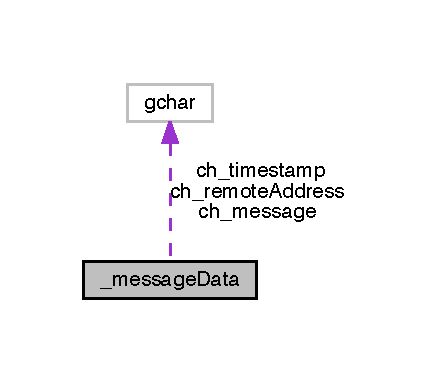
\includegraphics[width=206pt]{struct__message_data__coll__graph}
\end{center}
\end{figure}
\subsection*{Data Fields}
\begin{DoxyCompactItemize}
\item 
gchar \hyperlink{struct__message_data_a34854aba2033bcf0a48c1915b84452bf}{ch\+\_\+timestamp} \mbox{[}\hyperlink{gtk_d_s_8c_ac08ad1b127f1c9743c5592ffb796423f}{S\+Z\+\_\+\+T\+I\+M\+E\+S\+T\+A\+M\+P\+\_\+\+B\+U\+F\+F}\mbox{]}
\item 
gchar \hyperlink{struct__message_data_ad7d54fd9c1f9c0f8f6592ba194d6106f}{ch\+\_\+remote\+Address} \mbox{[}\hyperlink{gtk_d_s_8c_a152ca8fa1a2eac39d1badafb6c6cef8c}{S\+Z\+\_\+\+R\+M\+T\+A\+D\+D\+R\+\_\+\+B\+U\+F\+F}\mbox{]}
\item 
gchar \hyperlink{struct__message_data_a26366c3de6b85c0312117e42a46093e8}{ch\+\_\+message} \mbox{[}\hyperlink{gtk_d_s_8c_ab5903aa853c3769389e570c8490feb1e}{S\+Z\+\_\+\+M\+E\+S\+S\+A\+G\+E\+\_\+\+B\+U\+F\+F}\mbox{]}
\end{DoxyCompactItemize}


\subsection{Detailed Description}


Definition at line 86 of file gtk\+D\+S.\+c.



\subsection{Field Documentation}
\hypertarget{struct__message_data_a26366c3de6b85c0312117e42a46093e8}{\index{\+\_\+message\+Data@{\+\_\+message\+Data}!ch\+\_\+message@{ch\+\_\+message}}
\index{ch\+\_\+message@{ch\+\_\+message}!\+\_\+message\+Data@{\+\_\+message\+Data}}
\subsubsection[{ch\+\_\+message}]{\setlength{\rightskip}{0pt plus 5cm}gchar \+\_\+message\+Data\+::ch\+\_\+message\mbox{[}{\bf S\+Z\+\_\+\+M\+E\+S\+S\+A\+G\+E\+\_\+\+B\+U\+F\+F}\mbox{]}}}\label{struct__message_data_a26366c3de6b85c0312117e42a46093e8}


Definition at line 89 of file gtk\+D\+S.\+c.



Referenced by cb\+\_\+udp\+\_\+comm\+\_\+request\+\_\+handler(), and ui\+\_\+add\+\_\+message\+\_\+entry().

\hypertarget{struct__message_data_ad7d54fd9c1f9c0f8f6592ba194d6106f}{\index{\+\_\+message\+Data@{\+\_\+message\+Data}!ch\+\_\+remote\+Address@{ch\+\_\+remote\+Address}}
\index{ch\+\_\+remote\+Address@{ch\+\_\+remote\+Address}!\+\_\+message\+Data@{\+\_\+message\+Data}}
\subsubsection[{ch\+\_\+remote\+Address}]{\setlength{\rightskip}{0pt plus 5cm}gchar \+\_\+message\+Data\+::ch\+\_\+remote\+Address\mbox{[}{\bf S\+Z\+\_\+\+R\+M\+T\+A\+D\+D\+R\+\_\+\+B\+U\+F\+F}\mbox{]}}}\label{struct__message_data_ad7d54fd9c1f9c0f8f6592ba194d6106f}


Definition at line 88 of file gtk\+D\+S.\+c.



Referenced by cb\+\_\+udp\+\_\+comm\+\_\+request\+\_\+handler(), and ui\+\_\+add\+\_\+message\+\_\+entry().

\hypertarget{struct__message_data_a34854aba2033bcf0a48c1915b84452bf}{\index{\+\_\+message\+Data@{\+\_\+message\+Data}!ch\+\_\+timestamp@{ch\+\_\+timestamp}}
\index{ch\+\_\+timestamp@{ch\+\_\+timestamp}!\+\_\+message\+Data@{\+\_\+message\+Data}}
\subsubsection[{ch\+\_\+timestamp}]{\setlength{\rightskip}{0pt plus 5cm}gchar \+\_\+message\+Data\+::ch\+\_\+timestamp\mbox{[}{\bf S\+Z\+\_\+\+T\+I\+M\+E\+S\+T\+A\+M\+P\+\_\+\+B\+U\+F\+F}\mbox{]}}}\label{struct__message_data_a34854aba2033bcf0a48c1915b84452bf}


Definition at line 87 of file gtk\+D\+S.\+c.



Referenced by cb\+\_\+udp\+\_\+comm\+\_\+request\+\_\+handler(), and ui\+\_\+add\+\_\+message\+\_\+entry().



The documentation for this struct was generated from the following file\+:\begin{DoxyCompactItemize}
\item 
gtk\+D\+S/\hyperlink{gtk_d_s_8c}{gtk\+D\+S.\+c}\end{DoxyCompactItemize}

\hypertarget{struct__registry_data}{}\section{\+\_\+registry\+Data Struct Reference}
\label{struct__registry_data}\index{\+\_\+registry\+Data@{\+\_\+registry\+Data}}


Collaboration diagram for \+\_\+registry\+Data\+:\nopagebreak
\begin{figure}[H]
\begin{center}
\leavevmode
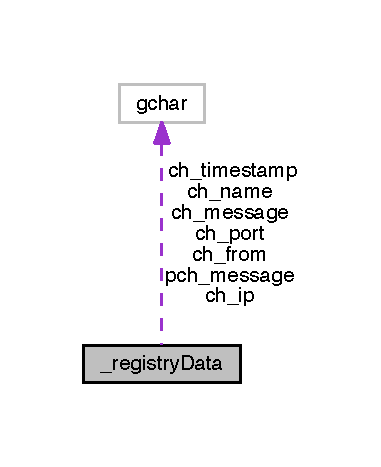
\includegraphics[width=183pt]{struct__registry_data__coll__graph}
\end{center}
\end{figure}
\subsection*{Data Fields}
\begin{DoxyCompactItemize}
\item 
gchar \hyperlink{struct__registry_data_a362a4edf89daafe79565053dd70892c4}{ch\+\_\+timestamp} \mbox{[}\hyperlink{gtk_d_s_8c_ac08ad1b127f1c9743c5592ffb796423f}{S\+Z\+\_\+\+T\+I\+M\+E\+S\+T\+A\+M\+P\+\_\+\+B\+U\+FF}\mbox{]}
\item 
gchar \hyperlink{struct__registry_data_a5fac46820690525a9d8b3f0185bca587}{ch\+\_\+from} \mbox{[}\hyperlink{gtk_d_s_8c_a152ca8fa1a2eac39d1badafb6c6cef8c}{S\+Z\+\_\+\+R\+M\+T\+A\+D\+D\+R\+\_\+\+B\+U\+FF}\mbox{]}
\item 
gchar \hyperlink{struct__registry_data_a4764e2a72c3ba9177b6c4803cfa03f72}{ch\+\_\+name} \mbox{[}\hyperlink{gtk_d_s_8c_a152ca8fa1a2eac39d1badafb6c6cef8c}{S\+Z\+\_\+\+R\+M\+T\+A\+D\+D\+R\+\_\+\+B\+U\+FF}\mbox{]}
\item 
gchar \hyperlink{struct__registry_data_a814e064e77a6aac5866c88cb51acd971}{ch\+\_\+ip} \mbox{[}\hyperlink{gtk_d_s_8c_ac21e8a77d073e7a5383c92bb485992c8}{S\+Z\+\_\+\+P\+A\+R\+A\+M\+S\+\_\+\+B\+U\+FF}\mbox{]}
\item 
gchar \hyperlink{struct__registry_data_a74f03616af9ec9770266cb7988fe1a71}{ch\+\_\+port} \mbox{[}\hyperlink{gtk_d_s_8c_ac21e8a77d073e7a5383c92bb485992c8}{S\+Z\+\_\+\+P\+A\+R\+A\+M\+S\+\_\+\+B\+U\+FF}\mbox{]}
\item 
gchar \hyperlink{struct__registry_data_aad089cfecaeccff2c9c6bb7a97d46706}{pch\+\_\+message} \mbox{[}\hyperlink{gtk_d_s_8c_ab5903aa853c3769389e570c8490feb1e}{S\+Z\+\_\+\+M\+E\+S\+S\+A\+G\+E\+\_\+\+B\+U\+FF}\mbox{]}
\item 
gchar \hyperlink{struct__registry_data_ae9b0c1e6f13d980dcc7515def6b20b5e}{ch\+\_\+message} \mbox{[}\hyperlink{gtk_d_s_8c_ab5903aa853c3769389e570c8490feb1e}{S\+Z\+\_\+\+M\+E\+S\+S\+A\+G\+E\+\_\+\+B\+U\+FF}\mbox{]}
\end{DoxyCompactItemize}


\subsection{Detailed Description}


Definition at line 81 of file cmd\+D\+C.\+c.



\subsection{Field Documentation}
\index{\+\_\+registry\+Data@{\+\_\+registry\+Data}!ch\+\_\+from@{ch\+\_\+from}}
\index{ch\+\_\+from@{ch\+\_\+from}!\+\_\+registry\+Data@{\+\_\+registry\+Data}}
\subsubsection[{\texorpdfstring{ch\+\_\+from}{ch_from}}]{\setlength{\rightskip}{0pt plus 5cm}gchar \+\_\+registry\+Data\+::ch\+\_\+from}\hypertarget{struct__registry_data_a5fac46820690525a9d8b3f0185bca587}{}\label{struct__registry_data_a5fac46820690525a9d8b3f0185bca587}


Definition at line 83 of file cmd\+D\+C.\+c.



Referenced by cb\+\_\+udp\+\_\+broadcast\+\_\+response\+\_\+handler(), and ui\+\_\+add\+\_\+registry\+\_\+entry().

\index{\+\_\+registry\+Data@{\+\_\+registry\+Data}!ch\+\_\+ip@{ch\+\_\+ip}}
\index{ch\+\_\+ip@{ch\+\_\+ip}!\+\_\+registry\+Data@{\+\_\+registry\+Data}}
\subsubsection[{\texorpdfstring{ch\+\_\+ip}{ch_ip}}]{\setlength{\rightskip}{0pt plus 5cm}gchar \+\_\+registry\+Data\+::ch\+\_\+ip}\hypertarget{struct__registry_data_a814e064e77a6aac5866c88cb51acd971}{}\label{struct__registry_data_a814e064e77a6aac5866c88cb51acd971}


Definition at line 85 of file cmd\+D\+C.\+c.



Referenced by cb\+\_\+udp\+\_\+broadcast\+\_\+response\+\_\+handler(), cb\+\_\+udp\+\_\+registry\+\_\+select\+\_\+handler(), udp\+\_\+registry\+\_\+response\+\_\+parser(), and ui\+\_\+add\+\_\+registry\+\_\+entry().

\index{\+\_\+registry\+Data@{\+\_\+registry\+Data}!ch\+\_\+message@{ch\+\_\+message}}
\index{ch\+\_\+message@{ch\+\_\+message}!\+\_\+registry\+Data@{\+\_\+registry\+Data}}
\subsubsection[{\texorpdfstring{ch\+\_\+message}{ch_message}}]{\setlength{\rightskip}{0pt plus 5cm}gchar \+\_\+registry\+Data\+::ch\+\_\+message}\hypertarget{struct__registry_data_ae9b0c1e6f13d980dcc7515def6b20b5e}{}\label{struct__registry_data_ae9b0c1e6f13d980dcc7515def6b20b5e}


Definition at line 80 of file cmd\+D\+S.\+c.



Referenced by cb\+\_\+udp\+\_\+broadcast\+\_\+response\+\_\+handler().

\index{\+\_\+registry\+Data@{\+\_\+registry\+Data}!ch\+\_\+name@{ch\+\_\+name}}
\index{ch\+\_\+name@{ch\+\_\+name}!\+\_\+registry\+Data@{\+\_\+registry\+Data}}
\subsubsection[{\texorpdfstring{ch\+\_\+name}{ch_name}}]{\setlength{\rightskip}{0pt plus 5cm}gchar \+\_\+registry\+Data\+::ch\+\_\+name}\hypertarget{struct__registry_data_a4764e2a72c3ba9177b6c4803cfa03f72}{}\label{struct__registry_data_a4764e2a72c3ba9177b6c4803cfa03f72}


Definition at line 84 of file cmd\+D\+C.\+c.



Referenced by cb\+\_\+udp\+\_\+broadcast\+\_\+response\+\_\+handler(), cb\+\_\+udp\+\_\+registry\+\_\+select\+\_\+handler(), udp\+\_\+registry\+\_\+find\+\_\+by\+\_\+name(), udp\+\_\+registry\+\_\+response\+\_\+parser(), and ui\+\_\+add\+\_\+registry\+\_\+entry().

\index{\+\_\+registry\+Data@{\+\_\+registry\+Data}!ch\+\_\+port@{ch\+\_\+port}}
\index{ch\+\_\+port@{ch\+\_\+port}!\+\_\+registry\+Data@{\+\_\+registry\+Data}}
\subsubsection[{\texorpdfstring{ch\+\_\+port}{ch_port}}]{\setlength{\rightskip}{0pt plus 5cm}gchar \+\_\+registry\+Data\+::ch\+\_\+port}\hypertarget{struct__registry_data_a74f03616af9ec9770266cb7988fe1a71}{}\label{struct__registry_data_a74f03616af9ec9770266cb7988fe1a71}


Definition at line 86 of file cmd\+D\+C.\+c.



Referenced by cb\+\_\+udp\+\_\+broadcast\+\_\+response\+\_\+handler(), cb\+\_\+udp\+\_\+registry\+\_\+select\+\_\+handler(), udp\+\_\+registry\+\_\+response\+\_\+parser(), and ui\+\_\+add\+\_\+registry\+\_\+entry().

\index{\+\_\+registry\+Data@{\+\_\+registry\+Data}!ch\+\_\+timestamp@{ch\+\_\+timestamp}}
\index{ch\+\_\+timestamp@{ch\+\_\+timestamp}!\+\_\+registry\+Data@{\+\_\+registry\+Data}}
\subsubsection[{\texorpdfstring{ch\+\_\+timestamp}{ch_timestamp}}]{\setlength{\rightskip}{0pt plus 5cm}gchar \+\_\+registry\+Data\+::ch\+\_\+timestamp}\hypertarget{struct__registry_data_a362a4edf89daafe79565053dd70892c4}{}\label{struct__registry_data_a362a4edf89daafe79565053dd70892c4}


Definition at line 82 of file cmd\+D\+C.\+c.



Referenced by cb\+\_\+udp\+\_\+broadcast\+\_\+response\+\_\+handler(), and ui\+\_\+add\+\_\+registry\+\_\+entry().

\index{\+\_\+registry\+Data@{\+\_\+registry\+Data}!pch\+\_\+message@{pch\+\_\+message}}
\index{pch\+\_\+message@{pch\+\_\+message}!\+\_\+registry\+Data@{\+\_\+registry\+Data}}
\subsubsection[{\texorpdfstring{pch\+\_\+message}{pch_message}}]{\setlength{\rightskip}{0pt plus 5cm}gchar \+\_\+registry\+Data\+::pch\+\_\+message}\hypertarget{struct__registry_data_aad089cfecaeccff2c9c6bb7a97d46706}{}\label{struct__registry_data_aad089cfecaeccff2c9c6bb7a97d46706}


Definition at line 87 of file cmd\+D\+C.\+c.



Referenced by cb\+\_\+udp\+\_\+broadcast\+\_\+response\+\_\+handler().



The documentation for this struct was generated from the following files\+:\begin{DoxyCompactItemize}
\item 
cmd\+D\+C/\hyperlink{cmd_d_c_8c}{cmd\+D\+C.\+c}\item 
cmd\+D\+S/\hyperlink{cmd_d_s_8c}{cmd\+D\+S.\+c}\item 
gssdp\+D\+C/\hyperlink{gssdp_d_c_8c}{gssdp\+D\+C.\+c}\item 
gtk\+D\+S/\hyperlink{gtk_d_s_8c}{gtk\+D\+S.\+c}\end{DoxyCompactItemize}

\hypertarget{struct__service_entry}{\section{\+\_\+service\+Entry Struct Reference}
\label{struct__service_entry}\index{\+\_\+service\+Entry@{\+\_\+service\+Entry}}
}


{\ttfamily \#include $<$skn\+\_\+common\+\_\+headers.\+h$>$}



Collaboration diagram for \+\_\+service\+Entry\+:\nopagebreak
\begin{figure}[H]
\begin{center}
\leavevmode
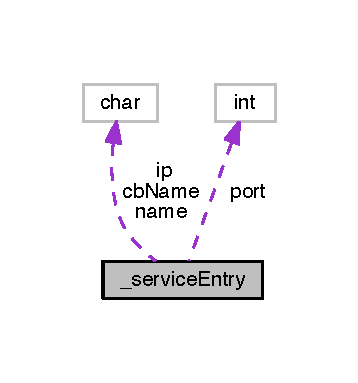
\includegraphics[width=172pt]{struct__service_entry__coll__graph}
\end{center}
\end{figure}
\subsection*{Data Fields}
\begin{DoxyCompactItemize}
\item 
char \hyperlink{struct__service_entry_ac654e9e33bf977ee6c36c46af83fbdd4}{cb\+Name} \mbox{[}\hyperlink{skn__common__headers_8h_a8d2978ad614b0de81c60483e706d9306}{S\+Z\+\_\+\+C\+H\+A\+R\+\_\+\+B\+U\+F\+F}\mbox{]}
\item 
char \hyperlink{struct__service_entry_aa66dcf0806f67276d049ac75c6153768}{name} \mbox{[}\hyperlink{skn__common__headers_8h_a442d5e93bd9c9d8eb4532aba62b5f86c}{S\+Z\+\_\+\+I\+N\+F\+O\+\_\+\+B\+U\+F\+F}\mbox{]}
\item 
char \hyperlink{struct__service_entry_a70b1db0895fbe31c07c8799cb57c678a}{ip} \mbox{[}\hyperlink{skn__common__headers_8h_a442d5e93bd9c9d8eb4532aba62b5f86c}{S\+Z\+\_\+\+I\+N\+F\+O\+\_\+\+B\+U\+F\+F}\mbox{]}
\item 
int \hyperlink{struct__service_entry_ac8a3a40de5eee937afb42faea4d18bb2}{port}
\end{DoxyCompactItemize}


\subsection{Detailed Description}


Definition at line 254 of file skn\+\_\+common\+\_\+headers.\+h.



\subsection{Field Documentation}
\hypertarget{struct__service_entry_ac654e9e33bf977ee6c36c46af83fbdd4}{\index{\+\_\+service\+Entry@{\+\_\+service\+Entry}!cb\+Name@{cb\+Name}}
\index{cb\+Name@{cb\+Name}!\+\_\+service\+Entry@{\+\_\+service\+Entry}}
\subsubsection[{cb\+Name}]{\setlength{\rightskip}{0pt plus 5cm}char \+\_\+service\+Entry\+::cb\+Name\mbox{[}{\bf S\+Z\+\_\+\+C\+H\+A\+R\+\_\+\+B\+U\+F\+F}\mbox{]}}}\label{struct__service_entry_ac654e9e33bf977ee6c36c46af83fbdd4}


Definition at line 255 of file skn\+\_\+common\+\_\+headers.\+h.



Referenced by skn\+\_\+service\+\_\+registry\+\_\+entry\+\_\+create().

\hypertarget{struct__service_entry_a70b1db0895fbe31c07c8799cb57c678a}{\index{\+\_\+service\+Entry@{\+\_\+service\+Entry}!ip@{ip}}
\index{ip@{ip}!\+\_\+service\+Entry@{\+\_\+service\+Entry}}
\subsubsection[{ip}]{\setlength{\rightskip}{0pt plus 5cm}char \+\_\+service\+Entry\+::ip\mbox{[}{\bf S\+Z\+\_\+\+I\+N\+F\+O\+\_\+\+B\+U\+F\+F}\mbox{]}}}\label{struct__service_entry_a70b1db0895fbe31c07c8799cb57c678a}


Definition at line 257 of file skn\+\_\+common\+\_\+headers.\+h.



Referenced by main(), skn\+\_\+service\+\_\+registry\+\_\+entry\+\_\+create(), skn\+\_\+service\+\_\+registry\+\_\+list\+\_\+entries(), and skn\+\_\+udp\+\_\+service\+\_\+request().

\hypertarget{struct__service_entry_aa66dcf0806f67276d049ac75c6153768}{\index{\+\_\+service\+Entry@{\+\_\+service\+Entry}!name@{name}}
\index{name@{name}!\+\_\+service\+Entry@{\+\_\+service\+Entry}}
\subsubsection[{name}]{\setlength{\rightskip}{0pt plus 5cm}char \+\_\+service\+Entry\+::name\mbox{[}{\bf S\+Z\+\_\+\+I\+N\+F\+O\+\_\+\+B\+U\+F\+F}\mbox{]}}}\label{struct__service_entry_aa66dcf0806f67276d049ac75c6153768}


Definition at line 256 of file skn\+\_\+common\+\_\+headers.\+h.



Referenced by main(), skn\+\_\+service\+\_\+registry\+\_\+entry\+\_\+create(), skn\+\_\+service\+\_\+registry\+\_\+find\+\_\+entry(), skn\+\_\+service\+\_\+registry\+\_\+list\+\_\+entries(), and skn\+\_\+udp\+\_\+service\+\_\+request().

\hypertarget{struct__service_entry_ac8a3a40de5eee937afb42faea4d18bb2}{\index{\+\_\+service\+Entry@{\+\_\+service\+Entry}!port@{port}}
\index{port@{port}!\+\_\+service\+Entry@{\+\_\+service\+Entry}}
\subsubsection[{port}]{\setlength{\rightskip}{0pt plus 5cm}int \+\_\+service\+Entry\+::port}}\label{struct__service_entry_ac8a3a40de5eee937afb42faea4d18bb2}


Definition at line 258 of file skn\+\_\+common\+\_\+headers.\+h.



Referenced by main(), skn\+\_\+service\+\_\+registry\+\_\+entry\+\_\+create(), skn\+\_\+service\+\_\+registry\+\_\+list\+\_\+entries(), and skn\+\_\+udp\+\_\+service\+\_\+request().



The documentation for this struct was generated from the following file\+:\begin{DoxyCompactItemize}
\item 
src/\hyperlink{skn__common__headers_8h}{skn\+\_\+common\+\_\+headers.\+h}\end{DoxyCompactItemize}

\hypertarget{struct__service_registry}{}\section{\+\_\+service\+Registry Struct Reference}
\label{struct__service_registry}\index{\+\_\+service\+Registry@{\+\_\+service\+Registry}}


{\ttfamily \#include $<$skn\+\_\+common\+\_\+headers.\+h$>$}



Collaboration diagram for \+\_\+service\+Registry\+:\nopagebreak
\begin{figure}[H]
\begin{center}
\leavevmode
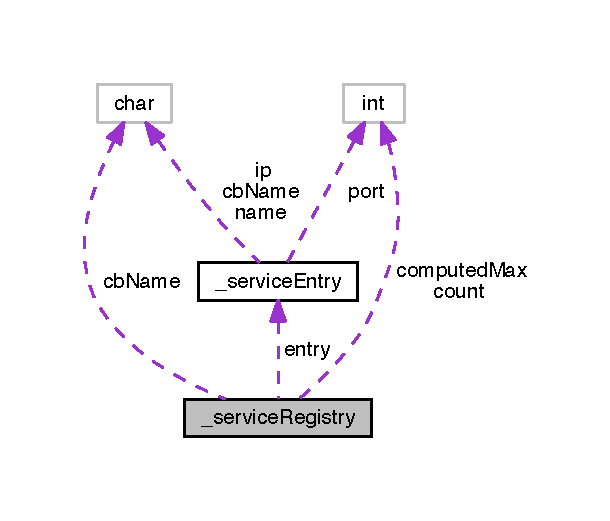
\includegraphics[width=293pt]{struct__service_registry__coll__graph}
\end{center}
\end{figure}
\subsection*{Data Fields}
\begin{DoxyCompactItemize}
\item 
char \hyperlink{struct__service_registry_ab822dc7bf25dc0eb498e81f81581e448}{cb\+Name} \mbox{[}\hyperlink{skn__common__headers_8h_a8d2978ad614b0de81c60483e706d9306}{S\+Z\+\_\+\+C\+H\+A\+R\+\_\+\+B\+U\+FF}\mbox{]}
\item 
int \hyperlink{struct__service_registry_a68062b14c6c9cb411e3602be664425bc}{count}
\item 
int \hyperlink{struct__service_registry_afc84b25f775a67d768cf4915db3c7115}{computed\+Max}
\item 
\hyperlink{skn__common__headers_8h_ac4f78e564b456af8e033cbc1275db23e}{P\+Registry\+Entry} \hyperlink{struct__service_registry_ad35429e298009925477ba528ea500fe8}{entry} \mbox{[}\hyperlink{skn__common__headers_8h_a0fd9cbccad9dcf96309b33d29862c83b}{A\+R\+Y\+\_\+\+M\+A\+X\+\_\+\+R\+E\+G\+I\+S\+T\+RY}\mbox{]}
\end{DoxyCompactItemize}


\subsection{Detailed Description}


Definition at line 261 of file skn\+\_\+common\+\_\+headers.\+h.



\subsection{Field Documentation}
\index{\+\_\+service\+Registry@{\+\_\+service\+Registry}!cb\+Name@{cb\+Name}}
\index{cb\+Name@{cb\+Name}!\+\_\+service\+Registry@{\+\_\+service\+Registry}}
\subsubsection[{\texorpdfstring{cb\+Name}{cbName}}]{\setlength{\rightskip}{0pt plus 5cm}char \+\_\+service\+Registry\+::cb\+Name\mbox{[}{\bf S\+Z\+\_\+\+C\+H\+A\+R\+\_\+\+B\+U\+FF}\mbox{]}}\hypertarget{struct__service_registry_ab822dc7bf25dc0eb498e81f81581e448}{}\label{struct__service_registry_ab822dc7bf25dc0eb498e81f81581e448}


Definition at line 262 of file skn\+\_\+common\+\_\+headers.\+h.



Referenced by service\+\_\+registry\+\_\+create().

\index{\+\_\+service\+Registry@{\+\_\+service\+Registry}!computed\+Max@{computed\+Max}}
\index{computed\+Max@{computed\+Max}!\+\_\+service\+Registry@{\+\_\+service\+Registry}}
\subsubsection[{\texorpdfstring{computed\+Max}{computedMax}}]{\setlength{\rightskip}{0pt plus 5cm}int \+\_\+service\+Registry\+::computed\+Max}\hypertarget{struct__service_registry_afc84b25f775a67d768cf4915db3c7115}{}\label{struct__service_registry_afc84b25f775a67d768cf4915db3c7115}


Definition at line 264 of file skn\+\_\+common\+\_\+headers.\+h.



Referenced by service\+\_\+registry\+\_\+create(), and service\+\_\+registry\+\_\+entry\+\_\+create().

\index{\+\_\+service\+Registry@{\+\_\+service\+Registry}!count@{count}}
\index{count@{count}!\+\_\+service\+Registry@{\+\_\+service\+Registry}}
\subsubsection[{\texorpdfstring{count}{count}}]{\setlength{\rightskip}{0pt plus 5cm}int \+\_\+service\+Registry\+::count}\hypertarget{struct__service_registry_a68062b14c6c9cb411e3602be664425bc}{}\label{struct__service_registry_a68062b14c6c9cb411e3602be664425bc}


Definition at line 263 of file skn\+\_\+common\+\_\+headers.\+h.



Referenced by service\+\_\+registry\+\_\+create(), service\+\_\+registry\+\_\+destroy(), service\+\_\+registry\+\_\+entry\+\_\+count(), service\+\_\+registry\+\_\+entry\+\_\+create(), service\+\_\+registry\+\_\+list\+\_\+entries(), and service\+\_\+registry\+\_\+response\+\_\+parse().

\index{\+\_\+service\+Registry@{\+\_\+service\+Registry}!entry@{entry}}
\index{entry@{entry}!\+\_\+service\+Registry@{\+\_\+service\+Registry}}
\subsubsection[{\texorpdfstring{entry}{entry}}]{\setlength{\rightskip}{0pt plus 5cm}{\bf P\+Registry\+Entry} \+\_\+service\+Registry\+::entry\mbox{[}{\bf A\+R\+Y\+\_\+\+M\+A\+X\+\_\+\+R\+E\+G\+I\+S\+T\+RY}\mbox{]}}\hypertarget{struct__service_registry_ad35429e298009925477ba528ea500fe8}{}\label{struct__service_registry_ad35429e298009925477ba528ea500fe8}


Definition at line 265 of file skn\+\_\+common\+\_\+headers.\+h.



Referenced by service\+\_\+registry\+\_\+create(), service\+\_\+registry\+\_\+destroy(), service\+\_\+registry\+\_\+entry\+\_\+create(), service\+\_\+registry\+\_\+find\+\_\+entry(), and service\+\_\+registry\+\_\+list\+\_\+entries().



The documentation for this struct was generated from the following file\+:\begin{DoxyCompactItemize}
\item 
src/\hyperlink{skn__common__headers_8h}{skn\+\_\+common\+\_\+headers.\+h}\end{DoxyCompactItemize}

\hypertarget{struct__service_request}{}\section{\+\_\+service\+Request Struct Reference}
\label{struct__service_request}\index{\+\_\+service\+Request@{\+\_\+service\+Request}}


{\ttfamily \#include $<$skn\+\_\+common\+\_\+headers.\+h$>$}



Collaboration diagram for \+\_\+service\+Request\+:
\nopagebreak
\begin{figure}[H]
\begin{center}
\leavevmode
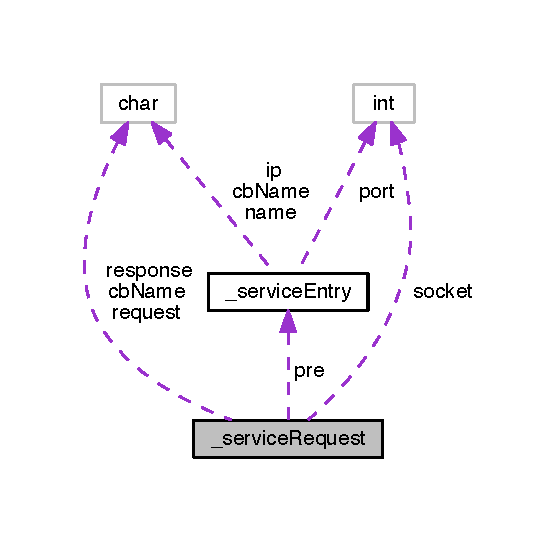
\includegraphics[width=267pt]{struct__service_request__coll__graph}
\end{center}
\end{figure}
\subsection*{Data Fields}
\begin{DoxyCompactItemize}
\item 
char \hyperlink{struct__service_request_aab7831722782ba05f0c94087598a941e}{cb\+Name} \mbox{[}\hyperlink{skn__common__headers_8h_a8d2978ad614b0de81c60483e706d9306}{S\+Z\+\_\+\+C\+H\+A\+R\+\_\+\+B\+U\+F\+F}\mbox{]}
\item 
\hyperlink{skn__common__headers_8h_ac4f78e564b456af8e033cbc1275db23e}{P\+Registry\+Entry} \hyperlink{struct__service_request_acf8d45e7f9cb65b555217aae74cd72c5}{pre}
\item 
char \hyperlink{struct__service_request_ad347b2a07388ec9d9d33756f1a1ef235}{request} \mbox{[}\hyperlink{skn__common__headers_8h_a442d5e93bd9c9d8eb4532aba62b5f86c}{S\+Z\+\_\+\+I\+N\+F\+O\+\_\+\+B\+U\+F\+F}\mbox{]}
\item 
char \hyperlink{struct__service_request_ad4e98b9d21fad17ba82dba6a9b5f6562}{response} \mbox{[}\hyperlink{skn__common__headers_8h_a442d5e93bd9c9d8eb4532aba62b5f86c}{S\+Z\+\_\+\+I\+N\+F\+O\+\_\+\+B\+U\+F\+F}\mbox{]}
\item 
int \hyperlink{struct__service_request_aa867fef3928c7511f50a494662311d13}{socket}
\end{DoxyCompactItemize}


\subsection{Detailed Description}


Definition at line 268 of file skn\+\_\+common\+\_\+headers.\+h.



\subsection{Field Documentation}
\hypertarget{struct__service_request_aab7831722782ba05f0c94087598a941e}{}\index{\+\_\+service\+Request@{\+\_\+service\+Request}!cb\+Name@{cb\+Name}}
\index{cb\+Name@{cb\+Name}!\+\_\+service\+Request@{\+\_\+service\+Request}}
\subsubsection[{cb\+Name}]{\setlength{\rightskip}{0pt plus 5cm}char \+\_\+service\+Request\+::cb\+Name\mbox{[}{\bf S\+Z\+\_\+\+C\+H\+A\+R\+\_\+\+B\+U\+F\+F}\mbox{]}}\label{struct__service_request_aab7831722782ba05f0c94087598a941e}


Definition at line 269 of file skn\+\_\+common\+\_\+headers.\+h.



Referenced by skn\+\_\+service\+\_\+request\+\_\+create().

\hypertarget{struct__service_request_acf8d45e7f9cb65b555217aae74cd72c5}{}\index{\+\_\+service\+Request@{\+\_\+service\+Request}!pre@{pre}}
\index{pre@{pre}!\+\_\+service\+Request@{\+\_\+service\+Request}}
\subsubsection[{pre}]{\setlength{\rightskip}{0pt plus 5cm}{\bf P\+Registry\+Entry} \+\_\+service\+Request\+::pre}\label{struct__service_request_acf8d45e7f9cb65b555217aae74cd72c5}


Definition at line 270 of file skn\+\_\+common\+\_\+headers.\+h.



Referenced by skn\+\_\+service\+\_\+request\+\_\+create(), and skn\+\_\+udp\+\_\+service\+\_\+request().

\hypertarget{struct__service_request_ad347b2a07388ec9d9d33756f1a1ef235}{}\index{\+\_\+service\+Request@{\+\_\+service\+Request}!request@{request}}
\index{request@{request}!\+\_\+service\+Request@{\+\_\+service\+Request}}
\subsubsection[{request}]{\setlength{\rightskip}{0pt plus 5cm}char \+\_\+service\+Request\+::request\mbox{[}{\bf S\+Z\+\_\+\+I\+N\+F\+O\+\_\+\+B\+U\+F\+F}\mbox{]}}\label{struct__service_request_ad347b2a07388ec9d9d33756f1a1ef235}


Definition at line 271 of file skn\+\_\+common\+\_\+headers.\+h.



Referenced by main(), skn\+\_\+service\+\_\+request\+\_\+create(), and skn\+\_\+udp\+\_\+service\+\_\+request().

\hypertarget{struct__service_request_ad4e98b9d21fad17ba82dba6a9b5f6562}{}\index{\+\_\+service\+Request@{\+\_\+service\+Request}!response@{response}}
\index{response@{response}!\+\_\+service\+Request@{\+\_\+service\+Request}}
\subsubsection[{response}]{\setlength{\rightskip}{0pt plus 5cm}char \+\_\+service\+Request\+::response\mbox{[}{\bf S\+Z\+\_\+\+I\+N\+F\+O\+\_\+\+B\+U\+F\+F}\mbox{]}}\label{struct__service_request_ad4e98b9d21fad17ba82dba6a9b5f6562}


Definition at line 272 of file skn\+\_\+common\+\_\+headers.\+h.



Referenced by skn\+\_\+udp\+\_\+service\+\_\+request().

\hypertarget{struct__service_request_aa867fef3928c7511f50a494662311d13}{}\index{\+\_\+service\+Request@{\+\_\+service\+Request}!socket@{socket}}
\index{socket@{socket}!\+\_\+service\+Request@{\+\_\+service\+Request}}
\subsubsection[{socket}]{\setlength{\rightskip}{0pt plus 5cm}int \+\_\+service\+Request\+::socket}\label{struct__service_request_aa867fef3928c7511f50a494662311d13}


Definition at line 273 of file skn\+\_\+common\+\_\+headers.\+h.



Referenced by skn\+\_\+service\+\_\+request\+\_\+create(), and skn\+\_\+udp\+\_\+service\+\_\+request().



The documentation for this struct was generated from the following file\+:\begin{DoxyCompactItemize}
\item 
src/\hyperlink{skn__common__headers_8h}{skn\+\_\+common\+\_\+headers.\+h}\end{DoxyCompactItemize}

\hypertarget{struct__signal_data}{}\section{\+\_\+signal\+Data Struct Reference}
\label{struct__signal_data}\index{\+\_\+signal\+Data@{\+\_\+signal\+Data}}


Collaboration diagram for \+\_\+signal\+Data\+:
\nopagebreak
\begin{figure}[H]
\begin{center}
\leavevmode
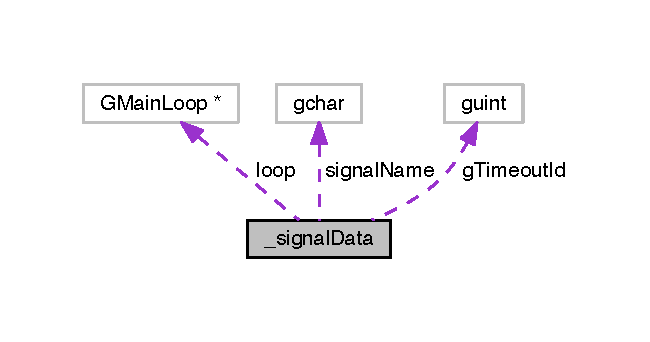
\includegraphics[width=312pt]{struct__signal_data__coll__graph}
\end{center}
\end{figure}
\subsection*{Data Fields}
\begin{DoxyCompactItemize}
\item 
G\+Main\+Loop $\ast$ \hyperlink{struct__signal_data_ae85864980ae30c1878e7149c26442544}{loop}
\item 
gchar $\ast$ \hyperlink{struct__signal_data_a6b2ce59a22a4ccc54e1d7a54e641d08f}{signal\+Name}
\item 
guint \hyperlink{struct__signal_data_adf058f0d9c77d84a462cc8eec963097b}{g\+Timeout\+Id}
\end{DoxyCompactItemize}


\subsection{Detailed Description}


Definition at line 76 of file cmd\+D\+C.\+c.



\subsection{Field Documentation}
\hypertarget{struct__signal_data_adf058f0d9c77d84a462cc8eec963097b}{}\index{\+\_\+signal\+Data@{\+\_\+signal\+Data}!g\+Timeout\+Id@{g\+Timeout\+Id}}
\index{g\+Timeout\+Id@{g\+Timeout\+Id}!\+\_\+signal\+Data@{\+\_\+signal\+Data}}
\subsubsection[{g\+Timeout\+Id}]{\setlength{\rightskip}{0pt plus 5cm}guint \+\_\+signal\+Data\+::g\+Timeout\+Id}\label{struct__signal_data_adf058f0d9c77d84a462cc8eec963097b}


Definition at line 84 of file cmd\+D\+S.\+c.

\hypertarget{struct__signal_data_ae85864980ae30c1878e7149c26442544}{}\index{\+\_\+signal\+Data@{\+\_\+signal\+Data}!loop@{loop}}
\index{loop@{loop}!\+\_\+signal\+Data@{\+\_\+signal\+Data}}
\subsubsection[{loop}]{\setlength{\rightskip}{0pt plus 5cm}G\+Main\+Loop $\ast$ \+\_\+signal\+Data\+::loop}\label{struct__signal_data_ae85864980ae30c1878e7149c26442544}


Definition at line 77 of file cmd\+D\+C.\+c.



Referenced by cb\+\_\+gtk\+\_\+shutdown(), cb\+\_\+unix\+\_\+signal\+\_\+handler(), and main().

\hypertarget{struct__signal_data_a6b2ce59a22a4ccc54e1d7a54e641d08f}{}\index{\+\_\+signal\+Data@{\+\_\+signal\+Data}!signal\+Name@{signal\+Name}}
\index{signal\+Name@{signal\+Name}!\+\_\+signal\+Data@{\+\_\+signal\+Data}}
\subsubsection[{signal\+Name}]{\setlength{\rightskip}{0pt plus 5cm}gchar $\ast$ \+\_\+signal\+Data\+::signal\+Name}\label{struct__signal_data_a6b2ce59a22a4ccc54e1d7a54e641d08f}


Definition at line 78 of file cmd\+D\+C.\+c.



Referenced by cb\+\_\+gtk\+\_\+shutdown(), cb\+\_\+unix\+\_\+signal\+\_\+handler(), and main().



The documentation for this struct was generated from the following files\+:\begin{DoxyCompactItemize}
\item 
cmd\+D\+C/\hyperlink{cmd_d_c_8c}{cmd\+D\+C.\+c}\item 
cmd\+D\+S/\hyperlink{cmd_d_s_8c}{cmd\+D\+S.\+c}\item 
gssdp\+D\+C/\hyperlink{gssdp_d_c_8c}{gssdp\+D\+C.\+c}\item 
gtk\+D\+S/\hyperlink{gtk_d_s_8c}{gtk\+D\+S.\+c}\end{DoxyCompactItemize}

\hypertarget{struct__temps}{}\section{\+\_\+temps Struct Reference}
\label{struct__temps}\index{\+\_\+temps@{\+\_\+temps}}


{\ttfamily \#include $<$skn\+\_\+common\+\_\+headers.\+h$>$}



Collaboration diagram for \+\_\+temps\+:
\nopagebreak
\begin{figure}[H]
\begin{center}
\leavevmode
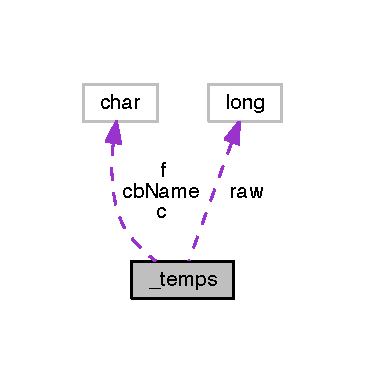
\includegraphics[width=175pt]{struct__temps__coll__graph}
\end{center}
\end{figure}
\subsection*{Data Fields}
\begin{DoxyCompactItemize}
\item 
char \hyperlink{struct__temps_a74414216b43459f4ebcada36b9b165f5}{cb\+Name} \mbox{[}\hyperlink{skn__common__headers_8h_a3122b900b1a34ceff868e0d51217e357}{S\+Z\+\_\+\+C\+H\+A\+R\+\_\+\+L\+A\+B\+E\+L}\mbox{]}
\item 
char \hyperlink{struct__temps_add683444c2985b00bd51bc69e9026a69}{c} \mbox{[}\hyperlink{skn__common__headers_8h_a3122b900b1a34ceff868e0d51217e357}{S\+Z\+\_\+\+C\+H\+A\+R\+\_\+\+L\+A\+B\+E\+L}\mbox{]}
\item 
char \hyperlink{struct__temps_a9de7d7f00c6df40b61735f25e3247b40}{f} \mbox{[}\hyperlink{skn__common__headers_8h_a3122b900b1a34ceff868e0d51217e357}{S\+Z\+\_\+\+C\+H\+A\+R\+\_\+\+L\+A\+B\+E\+L}\mbox{]}
\item 
long \hyperlink{struct__temps_a62d3522782b91f7fbb444bceb91c1876}{raw}
\end{DoxyCompactItemize}


\subsection{Detailed Description}


Definition at line 280 of file skn\+\_\+common\+\_\+headers.\+h.



\subsection{Field Documentation}
\hypertarget{struct__temps_add683444c2985b00bd51bc69e9026a69}{}\index{\+\_\+temps@{\+\_\+temps}!c@{c}}
\index{c@{c}!\+\_\+temps@{\+\_\+temps}}
\subsubsection[{c}]{\setlength{\rightskip}{0pt plus 5cm}char \+\_\+temps\+::c\mbox{[}{\bf S\+Z\+\_\+\+C\+H\+A\+R\+\_\+\+L\+A\+B\+E\+L}\mbox{]}}\label{struct__temps_add683444c2985b00bd51bc69e9026a69}


Definition at line 282 of file skn\+\_\+common\+\_\+headers.\+h.



Referenced by generate\+\_\+cpu\+\_\+temps\+\_\+info(), and get\+Cpu\+Temps().

\hypertarget{struct__temps_a74414216b43459f4ebcada36b9b165f5}{}\index{\+\_\+temps@{\+\_\+temps}!cb\+Name@{cb\+Name}}
\index{cb\+Name@{cb\+Name}!\+\_\+temps@{\+\_\+temps}}
\subsubsection[{cb\+Name}]{\setlength{\rightskip}{0pt plus 5cm}char \+\_\+temps\+::cb\+Name\mbox{[}{\bf S\+Z\+\_\+\+C\+H\+A\+R\+\_\+\+L\+A\+B\+E\+L}\mbox{]}}\label{struct__temps_a74414216b43459f4ebcada36b9b165f5}


Definition at line 281 of file skn\+\_\+common\+\_\+headers.\+h.



Referenced by get\+Cpu\+Temps().

\hypertarget{struct__temps_a9de7d7f00c6df40b61735f25e3247b40}{}\index{\+\_\+temps@{\+\_\+temps}!f@{f}}
\index{f@{f}!\+\_\+temps@{\+\_\+temps}}
\subsubsection[{f}]{\setlength{\rightskip}{0pt plus 5cm}char \+\_\+temps\+::f\mbox{[}{\bf S\+Z\+\_\+\+C\+H\+A\+R\+\_\+\+L\+A\+B\+E\+L}\mbox{]}}\label{struct__temps_a9de7d7f00c6df40b61735f25e3247b40}


Definition at line 283 of file skn\+\_\+common\+\_\+headers.\+h.



Referenced by generate\+\_\+cpu\+\_\+temps\+\_\+info(), and get\+Cpu\+Temps().

\hypertarget{struct__temps_a62d3522782b91f7fbb444bceb91c1876}{}\index{\+\_\+temps@{\+\_\+temps}!raw@{raw}}
\index{raw@{raw}!\+\_\+temps@{\+\_\+temps}}
\subsubsection[{raw}]{\setlength{\rightskip}{0pt plus 5cm}long \+\_\+temps\+::raw}\label{struct__temps_a62d3522782b91f7fbb444bceb91c1876}


Definition at line 284 of file skn\+\_\+common\+\_\+headers.\+h.



Referenced by get\+Cpu\+Temps().



The documentation for this struct was generated from the following file\+:\begin{DoxyCompactItemize}
\item 
src/\hyperlink{skn__common__headers_8h}{skn\+\_\+common\+\_\+headers.\+h}\end{DoxyCompactItemize}

\hypertarget{struct_message_queue_source}{}\section{Message\+Queue\+Source Struct Reference}
\label{struct_message_queue_source}\index{Message\+Queue\+Source@{Message\+Queue\+Source}}


Collaboration diagram for Message\+Queue\+Source\+:\nopagebreak
\begin{figure}[H]
\begin{center}
\leavevmode
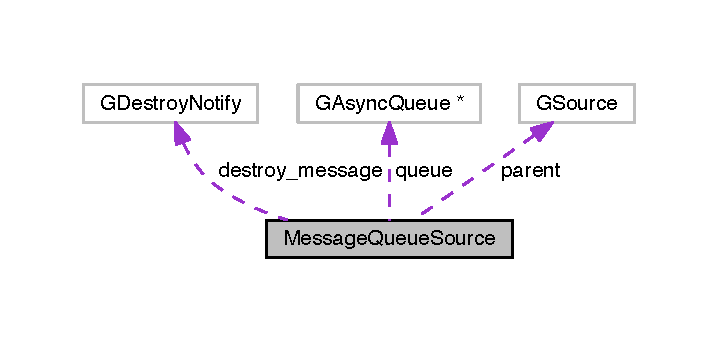
\includegraphics[width=345pt]{struct_message_queue_source__coll__graph}
\end{center}
\end{figure}
\subsection*{Data Fields}
\begin{DoxyCompactItemize}
\item 
G\+Source \hyperlink{struct_message_queue_source_a3c77a6e5fe65c6db7f6c2f0352b4f381}{parent}
\item 
G\+Async\+Queue $\ast$ \hyperlink{struct_message_queue_source_ad1652a95a0056320f7a84a139829b770}{queue}
\item 
G\+Destroy\+Notify \hyperlink{struct_message_queue_source_acf4671d25f6351d60e7a852e752d5ccc}{destroy\+\_\+message}
\end{DoxyCompactItemize}


\subsection{Detailed Description}
\hyperlink{struct_message_queue_source}{Message\+Queue\+Source}\+:

Ref\+: \href{https://developer.gnome.org/gnome-devel-demos/stable/custom-gsource.c.html.en}{\tt https\+://developer.\+gnome.\+org/gnome-\/devel-\/demos/stable/custom-\/gsource.\+c.\+html.\+en}

This is a \#\+G\+Source which wraps a \#\+G\+Async\+Queue and is dispatched whenever a message can be pulled off the queue. Messages can be enqueued from any thread.

The callbacks dispatched by a \hyperlink{struct_message_queue_source}{Message\+Queue\+Source} have type \hyperlink{gtk_d_s_8c_ac3dbd4bd01ae030fdaba57baa498e712}{Message\+Queue\+Source\+Func}.

\hyperlink{struct_message_queue_source}{Message\+Queue\+Source} supports adding a \#\+G\+Cancellable child source which will additionally dispatch if a provided \#\+G\+Cancellable is cancelled. 

Definition at line 221 of file gtk\+D\+S.\+c.



\subsection{Field Documentation}
\index{Message\+Queue\+Source@{Message\+Queue\+Source}!destroy\+\_\+message@{destroy\+\_\+message}}
\index{destroy\+\_\+message@{destroy\+\_\+message}!Message\+Queue\+Source@{Message\+Queue\+Source}}
\subsubsection[{\texorpdfstring{destroy\+\_\+message}{destroy_message}}]{\setlength{\rightskip}{0pt plus 5cm}G\+Destroy\+Notify Message\+Queue\+Source\+::destroy\+\_\+message}\hypertarget{struct_message_queue_source_acf4671d25f6351d60e7a852e752d5ccc}{}\label{struct_message_queue_source_acf4671d25f6351d60e7a852e752d5ccc}


Definition at line 224 of file gtk\+D\+S.\+c.



Referenced by message\+\_\+queue\+\_\+source\+\_\+dispatch(), and message\+\_\+queue\+\_\+source\+\_\+new().

\index{Message\+Queue\+Source@{Message\+Queue\+Source}!parent@{parent}}
\index{parent@{parent}!Message\+Queue\+Source@{Message\+Queue\+Source}}
\subsubsection[{\texorpdfstring{parent}{parent}}]{\setlength{\rightskip}{0pt plus 5cm}G\+Source Message\+Queue\+Source\+::parent}\hypertarget{struct_message_queue_source_a3c77a6e5fe65c6db7f6c2f0352b4f381}{}\label{struct_message_queue_source_a3c77a6e5fe65c6db7f6c2f0352b4f381}


Definition at line 222 of file gtk\+D\+S.\+c.

\index{Message\+Queue\+Source@{Message\+Queue\+Source}!queue@{queue}}
\index{queue@{queue}!Message\+Queue\+Source@{Message\+Queue\+Source}}
\subsubsection[{\texorpdfstring{queue}{queue}}]{\setlength{\rightskip}{0pt plus 5cm}G\+Async\+Queue$\ast$ Message\+Queue\+Source\+::queue}\hypertarget{struct_message_queue_source_ad1652a95a0056320f7a84a139829b770}{}\label{struct_message_queue_source_ad1652a95a0056320f7a84a139829b770}


Definition at line 223 of file gtk\+D\+S.\+c.



Referenced by message\+\_\+queue\+\_\+source\+\_\+dispatch(), message\+\_\+queue\+\_\+source\+\_\+finalize(), message\+\_\+queue\+\_\+source\+\_\+new(), and message\+\_\+queue\+\_\+source\+\_\+prepare().



The documentation for this struct was generated from the following file\+:\begin{DoxyCompactItemize}
\item 
gtk\+D\+S/\hyperlink{gtk_d_s_8c}{gtk\+D\+S.\+c}\end{DoxyCompactItemize}

\chapter{File Documentation}
\hypertarget{cmd_d_c_8c}{}\section{cmd\+D\+C/cmd\+D\+C.c File Reference}
\label{cmd_d_c_8c}\index{cmd\+D\+C/cmd\+D\+C.\+c@{cmd\+D\+C/cmd\+D\+C.\+c}}
{\ttfamily \#include $<$stdlib.\+h$>$}\\*
{\ttfamily \#include $<$stdio.\+h$>$}\\*
{\ttfamily \#include $<$string.\+h$>$}\\*
{\ttfamily \#include $<$glib.\+h$>$}\\*
{\ttfamily \#include $<$gio/gio.\+h$>$}\\*
{\ttfamily \#include $<$glib-\/unix.\+h$>$}\\*
{\ttfamily \#include $<$gio/gnetworking.\+h$>$}\\*
{\ttfamily \#include $<$ifaddrs.\+h$>$}\\*
Include dependency graph for cmd\+D\+C.\+c\+:
\nopagebreak
\begin{figure}[H]
\begin{center}
\leavevmode
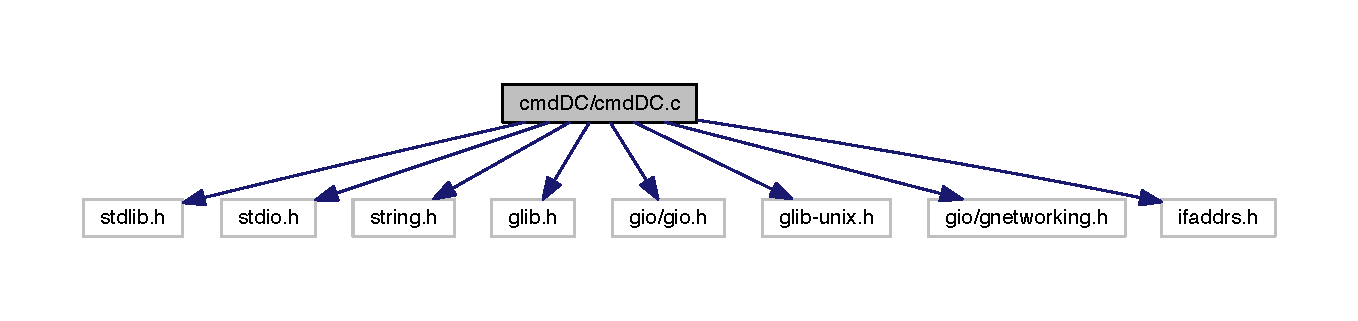
\includegraphics[width=350pt]{cmd_d_c_8c__incl}
\end{center}
\end{figure}
\subsection*{Data Structures}
\begin{DoxyCompactItemize}
\item 
struct \hyperlink{struct__ip_broadcast_array}{\+\_\+ip\+Broadcast\+Array}
\item 
struct \hyperlink{struct__signal_data}{\+\_\+signal\+Data}
\item 
struct \hyperlink{struct__registry_data}{\+\_\+registry\+Data}
\item 
struct \hyperlink{struct__control_data}{\+\_\+control\+Data}
\end{DoxyCompactItemize}
\subsection*{Macros}
\begin{DoxyCompactItemize}
\item 
\#define \hyperlink{cmd_d_c_8c_aa326a05d5e30f9e9a4bb0b4469d5d0c0}{P\+A\+C\+K\+A\+G\+E\+\_\+\+V\+E\+R\+S\+I\+O\+N}~\char`\"{}0.\+9.\+0\char`\"{}
\item 
\#define \hyperlink{cmd_d_c_8c_a1c0439e4355794c09b64274849eb0279}{P\+A\+C\+K\+A\+G\+E\+\_\+\+N\+A\+M\+E}~\char`\"{}cmd\+D\+C\char`\"{}
\item 
\#define \hyperlink{cmd_d_c_8c_a714627d9e7b71b55548e2ddda429d3fb}{P\+A\+C\+K\+A\+G\+E\+\_\+\+D\+E\+S\+C\+R\+I\+P\+T\+I\+O\+N}~\char`\"{}Send Message to Raspberry Pi\textquotesingle{}s on the network.\char`\"{}
\item 
\#define \hyperlink{cmd_d_c_8c_a8e8475ded7103e72515667b568ed64c7}{G\+\_\+\+O\+P\+T\+I\+O\+N\+\_\+\+F\+L\+A\+G\+\_\+\+N\+O\+N\+E}~0
\item 
\#define \hyperlink{cmd_d_c_8c_adf765361163d05006ff697149bbaf2ee}{U\+D\+P\+\_\+\+D\+I\+S\+P\+L\+A\+Y\+\_\+\+C\+O\+M\+M\+\_\+\+P\+O\+R\+T}~48029
\item 
\#define \hyperlink{cmd_d_c_8c_a76bd5a574aad0fa67de6c9804853f191}{U\+D\+P\+\_\+\+B\+R\+O\+A\+D\+C\+A\+S\+T\+\_\+\+P\+O\+R\+T}~48028
\item 
\#define \hyperlink{cmd_d_c_8c_af16df2ad6ba0bf1f5283361eb89a979d}{U\+D\+P\+\_\+\+R\+E\+G\+U\+L\+A\+R\+\_\+\+P\+O\+R\+T}~48027
\item 
\#define \hyperlink{cmd_d_c_8c_aeed5f98eabe9b11442a6fe0aad5b5be0}{U\+D\+P\+\_\+\+C\+L\+I\+E\+N\+T\+S\+\_\+\+P\+O\+R\+T}~48026
\item 
\#define \hyperlink{cmd_d_c_8c_ac10012e31213e44ecaf5d4c1dd3c8719}{M\+S\+\_\+\+T\+E\+N\+\_\+\+M\+I\+N\+U\+T\+E\+S}~600000
\item 
\#define \hyperlink{cmd_d_c_8c_ac66d92e429586a7c5d0424fe6ad105dd}{M\+S\+G\+\_\+\+D\+E\+L\+A\+Y\+\_\+\+I\+N\+T\+E\+R\+V\+A\+L}~10
\item 
\#define \hyperlink{cmd_d_c_8c_ac08ad1b127f1c9743c5592ffb796423f}{S\+Z\+\_\+\+T\+I\+M\+E\+S\+T\+A\+M\+P\+\_\+\+B\+U\+F\+F}~32
\item 
\#define \hyperlink{cmd_d_c_8c_ac21e8a77d073e7a5383c92bb485992c8}{S\+Z\+\_\+\+P\+A\+R\+A\+M\+S\+\_\+\+B\+U\+F\+F}~64
\item 
\#define \hyperlink{cmd_d_c_8c_a152ca8fa1a2eac39d1badafb6c6cef8c}{S\+Z\+\_\+\+R\+M\+T\+A\+D\+D\+R\+\_\+\+B\+U\+F\+F}~256
\item 
\#define \hyperlink{cmd_d_c_8c_ab5903aa853c3769389e570c8490feb1e}{S\+Z\+\_\+\+M\+E\+S\+S\+A\+G\+E\+\_\+\+B\+U\+F\+F}~512
\item 
\#define \hyperlink{cmd_d_c_8c_a3c73a8961a16a0dfbb87b5a7317bacd2}{S\+Z\+\_\+\+R\+E\+S\+P\+O\+N\+S\+E\+\_\+\+B\+U\+F\+F}~256
\item 
\#define \hyperlink{cmd_d_c_8c_a3122b900b1a34ceff868e0d51217e357}{S\+Z\+\_\+\+C\+H\+A\+R\+\_\+\+L\+A\+B\+E\+L}~48
\item 
\#define \hyperlink{cmd_d_c_8c_a442d5e93bd9c9d8eb4532aba62b5f86c}{S\+Z\+\_\+\+I\+N\+F\+O\+\_\+\+B\+U\+F\+F}~256
\item 
\#define \hyperlink{cmd_d_c_8c_a8d2978ad614b0de81c60483e706d9306}{S\+Z\+\_\+\+C\+H\+A\+R\+\_\+\+B\+U\+F\+F}~128
\item 
\#define \hyperlink{cmd_d_c_8c_a77ca0b062f899750ee20c0170e5bedc4}{S\+Z\+\_\+\+L\+I\+N\+E\+\_\+\+B\+U\+F\+F}~512
\item 
\#define \hyperlink{cmd_d_c_8c_a352051a682a5205841c1bda6e30bb30d}{S\+Z\+\_\+\+C\+O\+M\+M\+\_\+\+B\+U\+F\+F}~256
\item 
\#define \hyperlink{cmd_d_c_8c_a8091fbaa709d661a678a82a62fab638b}{S\+K\+N\+\_\+\+U\+D\+P\+\_\+\+A\+N\+Y\+\_\+\+P\+O\+R\+T}~0
\item 
\#define \hyperlink{cmd_d_c_8c_a00b19837422a3b13d82b9a525e92ef51}{A\+R\+Y\+\_\+\+M\+A\+X\+\_\+\+I\+N\+T\+F}~8
\item 
\#define \hyperlink{cmd_d_c_8c_a12efd06fda89d6826f820e75148d8fd7}{P\+L\+A\+T\+F\+O\+R\+M\+\_\+\+E\+R\+R\+O\+R}~-\/1
\end{DoxyCompactItemize}
\subsection*{Typedefs}
\begin{DoxyCompactItemize}
\item 
typedef struct \hyperlink{struct__ip_broadcast_array}{\+\_\+ip\+Broadcast\+Array} \hyperlink{cmd_d_c_8c_a83c26957f648dd04df183020ab03c60d}{I\+P\+Broadcast\+Array}
\item 
typedef struct \hyperlink{struct__ip_broadcast_array}{\+\_\+ip\+Broadcast\+Array} $\ast$ \hyperlink{cmd_d_c_8c_a916d712cacebc2faeda930352280c361}{P\+I\+P\+Broadcast\+Array}
\item 
typedef struct \hyperlink{struct__signal_data}{\+\_\+signal\+Data} \hyperlink{cmd_d_c_8c_a4d86cbb761613143e4ee60218efdfbaa}{U\+Signal\+Data}
\item 
typedef struct \hyperlink{struct__signal_data}{\+\_\+signal\+Data} $\ast$ \hyperlink{cmd_d_c_8c_acdc6976ac4ccc0f13bc99bb5b9361a6e}{P\+U\+Signal\+Data}
\item 
typedef struct \hyperlink{struct__registry_data}{\+\_\+registry\+Data} \hyperlink{cmd_d_c_8c_aac252e0f10021267858720b8e772c0fc}{Reg\+Data}
\item 
typedef struct \hyperlink{struct__registry_data}{\+\_\+registry\+Data} $\ast$ \hyperlink{cmd_d_c_8c_a57f677cfc01b955d9d3783e5422f36a8}{P\+Reg\+Data}
\item 
typedef struct \hyperlink{struct__registry_data}{\+\_\+registry\+Data} $\ast$$\ast$ \hyperlink{cmd_d_c_8c_a0b249e07431f112b20e1708c3162d8a0}{P\+P\+Reg\+Data}
\item 
typedef struct \hyperlink{struct__control_data}{\+\_\+control\+Data} \hyperlink{cmd_d_c_8c_aad121cd36cd8851b2a3cd81fd0e41388}{Control\+Data}
\item 
typedef struct \hyperlink{struct__control_data}{\+\_\+control\+Data} $\ast$ \hyperlink{cmd_d_c_8c_aa6bae802f1b23385cd660e89a1e4fc75}{P\+Control\+Data}
\end{DoxyCompactItemize}
\subsection*{Functions}
\begin{DoxyCompactItemize}
\item 
gchar $\ast$ \hyperlink{cmd_d_c_8c_a8288aea959581188e5bd29430935a6ed}{skn\+\_\+get\+\_\+timestamp} ()
\item 
gint \hyperlink{cmd_d_c_8c_ae59da66ef51690f71da087514886fd12}{udp\+\_\+registry\+\_\+find\+\_\+by\+\_\+name} (\hyperlink{cmd_d_c_8c_a57f677cfc01b955d9d3783e5422f36a8}{P\+Reg\+Data} pr, gchar $\ast$pch\+\_\+name)
\item 
\hyperlink{cmd_d_c_8c_a0b249e07431f112b20e1708c3162d8a0}{P\+P\+Reg\+Data} \hyperlink{cmd_d_c_8c_a568a9919cfd345f6c1a41a2ec7c4b1ca}{udp\+\_\+registry\+\_\+response\+\_\+parser} (\hyperlink{cmd_d_c_8c_a57f677cfc01b955d9d3783e5422f36a8}{P\+Reg\+Data} msg, gchar $\ast$response)
\item 
gchar $\ast$ \hyperlink{cmd_d_c_8c_af4d9de57a3cb296036c837a644009ef5}{skn\+\_\+gio\+\_\+condition\+\_\+to\+\_\+string} (G\+I\+O\+Condition condition)
\item 
gboolean \hyperlink{cmd_d_c_8c_a793c6b3e5c7a5abc993d8cfbe963629d}{udp\+\_\+initialize\+\_\+message\+\_\+send} (\hyperlink{cmd_d_c_8c_aa6bae802f1b23385cd660e89a1e4fc75}{P\+Control\+Data} pctrl)
\item 
static gboolean \hyperlink{cmd_d_c_8c_a76ad4de5945cff6e20dbeff46bda868b}{cb\+\_\+unix\+\_\+signal\+\_\+handler} (\hyperlink{cmd_d_c_8c_acdc6976ac4ccc0f13bc99bb5b9361a6e}{P\+U\+Signal\+Data} psig)
\item 
static gboolean \hyperlink{cmd_d_c_8c_a00c5b52bdcb7caec07d08b05b8c1dced}{cb\+\_\+udp\+\_\+comm\+\_\+request\+\_\+handler} (\hyperlink{cmd_d_c_8c_aa6bae802f1b23385cd660e89a1e4fc75}{P\+Control\+Data} pctrl)
\item 
static gboolean \hyperlink{cmd_d_c_8c_aa8a19e68e54683fa324bcee1ecfd3942}{cb\+\_\+udp\+\_\+comm\+\_\+response\+\_\+handler} (G\+Socket $\ast$g\+Sock, G\+I\+O\+Condition condition, \hyperlink{cmd_d_c_8c_aa6bae802f1b23385cd660e89a1e4fc75}{P\+Control\+Data} pctrl)
\item 
static gboolean \hyperlink{cmd_d_c_8c_a385b710fd30ba190b3b96e814424ff80}{cb\+\_\+udp\+\_\+broadcast\+\_\+response\+\_\+handler} (G\+Socket $\ast$g\+Sock, G\+I\+O\+Condition condition, \hyperlink{cmd_d_c_8c_aa6bae802f1b23385cd660e89a1e4fc75}{P\+Control\+Data} pctrl)
\item 
static gboolean \hyperlink{cmd_d_c_8c_a160bb2056d3842ef84fd7211ed6ec385}{cb\+\_\+udp\+\_\+registry\+\_\+select\+\_\+handler} (\hyperlink{cmd_d_c_8c_aa6bae802f1b23385cd660e89a1e4fc75}{P\+Control\+Data} pctrl)
\item 
\hyperlink{cmd_d_c_8c_a916d712cacebc2faeda930352280c361}{P\+I\+P\+Broadcast\+Array} \hyperlink{cmd_d_c_8c_a72be87baa67e532c78af054acf935d6c}{skn\+\_\+get\+\_\+default\+\_\+interface\+\_\+name\+\_\+and\+\_\+ipv4\+\_\+address} (char $\ast$intf, char $\ast$ipv4)
\item 
gint \hyperlink{cmd_d_c_8c_a0dfc1a6916909805dc7fd2d8c471e0e3}{skn\+\_\+get\+\_\+broadcast\+\_\+ip\+\_\+array} (\hyperlink{cmd_d_c_8c_a916d712cacebc2faeda930352280c361}{P\+I\+P\+Broadcast\+Array} pa\+B)
\item 
gint \hyperlink{cmd_d_c_8c_afc164e6efc7bdcdbacba97ba6f6c2a19}{skn\+\_\+get\+\_\+default\+\_\+interface\+\_\+name} (char $\ast$pch\+Default\+Interface\+Name)
\item 
gboolean \hyperlink{cmd_d_c_8c_af376243f65a3fd761050836d1293b0d9}{skn\+\_\+udp\+\_\+network\+\_\+broadcast\+\_\+all\+\_\+interfaces} (G\+Socket $\ast$g\+Sock, \hyperlink{cmd_d_c_8c_a916d712cacebc2faeda930352280c361}{P\+I\+P\+Broadcast\+Array} pab)
\item 
gchar $\ast$ \hyperlink{cmd_d_c_8c_a73ed6790a0276f43dfea595f4cedffa4}{skn\+\_\+strip} (gchar $\ast$alpha)
\item 
\hyperlink{cmd_d_c_8c_a916d712cacebc2faeda930352280c361}{P\+I\+P\+Broadcast\+Array} \hyperlink{cmd_d_c_8c_a4f733621137368e762c5db74a3cec52b}{skn\+\_\+get\+\_\+default\+\_\+interface\+\_\+name\+\_\+and\+\_\+ipv4\+\_\+address} (gchar $\ast$intf, gchar $\ast$ipv4)
\item 
int \hyperlink{cmd_d_c_8c_a3c04138a5bfe5d72780bb7e82a18e627}{main} (int argc, char $\ast$$\ast$argv)
\end{DoxyCompactItemize}


\subsection{Macro Definition Documentation}
\hypertarget{cmd_d_c_8c_a00b19837422a3b13d82b9a525e92ef51}{}\index{cmd\+D\+C.\+c@{cmd\+D\+C.\+c}!A\+R\+Y\+\_\+\+M\+A\+X\+\_\+\+I\+N\+T\+F@{A\+R\+Y\+\_\+\+M\+A\+X\+\_\+\+I\+N\+T\+F}}
\index{A\+R\+Y\+\_\+\+M\+A\+X\+\_\+\+I\+N\+T\+F@{A\+R\+Y\+\_\+\+M\+A\+X\+\_\+\+I\+N\+T\+F}!cmd\+D\+C.\+c@{cmd\+D\+C.\+c}}
\subsubsection[{A\+R\+Y\+\_\+\+M\+A\+X\+\_\+\+I\+N\+T\+F}]{\setlength{\rightskip}{0pt plus 5cm}\#define A\+R\+Y\+\_\+\+M\+A\+X\+\_\+\+I\+N\+T\+F~8}\label{cmd_d_c_8c_a00b19837422a3b13d82b9a525e92ef51}


Definition at line 62 of file cmd\+D\+C.\+c.



Referenced by get\+\_\+broadcast\+\_\+ip\+\_\+array(), and skn\+\_\+get\+\_\+broadcast\+\_\+ip\+\_\+array().

\hypertarget{cmd_d_c_8c_a8e8475ded7103e72515667b568ed64c7}{}\index{cmd\+D\+C.\+c@{cmd\+D\+C.\+c}!G\+\_\+\+O\+P\+T\+I\+O\+N\+\_\+\+F\+L\+A\+G\+\_\+\+N\+O\+N\+E@{G\+\_\+\+O\+P\+T\+I\+O\+N\+\_\+\+F\+L\+A\+G\+\_\+\+N\+O\+N\+E}}
\index{G\+\_\+\+O\+P\+T\+I\+O\+N\+\_\+\+F\+L\+A\+G\+\_\+\+N\+O\+N\+E@{G\+\_\+\+O\+P\+T\+I\+O\+N\+\_\+\+F\+L\+A\+G\+\_\+\+N\+O\+N\+E}!cmd\+D\+C.\+c@{cmd\+D\+C.\+c}}
\subsubsection[{G\+\_\+\+O\+P\+T\+I\+O\+N\+\_\+\+F\+L\+A\+G\+\_\+\+N\+O\+N\+E}]{\setlength{\rightskip}{0pt plus 5cm}\#define G\+\_\+\+O\+P\+T\+I\+O\+N\+\_\+\+F\+L\+A\+G\+\_\+\+N\+O\+N\+E~0}\label{cmd_d_c_8c_a8e8475ded7103e72515667b568ed64c7}


Definition at line 38 of file cmd\+D\+C.\+c.



Referenced by main().

\hypertarget{cmd_d_c_8c_ac10012e31213e44ecaf5d4c1dd3c8719}{}\index{cmd\+D\+C.\+c@{cmd\+D\+C.\+c}!M\+S\+\_\+\+T\+E\+N\+\_\+\+M\+I\+N\+U\+T\+E\+S@{M\+S\+\_\+\+T\+E\+N\+\_\+\+M\+I\+N\+U\+T\+E\+S}}
\index{M\+S\+\_\+\+T\+E\+N\+\_\+\+M\+I\+N\+U\+T\+E\+S@{M\+S\+\_\+\+T\+E\+N\+\_\+\+M\+I\+N\+U\+T\+E\+S}!cmd\+D\+C.\+c@{cmd\+D\+C.\+c}}
\subsubsection[{M\+S\+\_\+\+T\+E\+N\+\_\+\+M\+I\+N\+U\+T\+E\+S}]{\setlength{\rightskip}{0pt plus 5cm}\#define M\+S\+\_\+\+T\+E\+N\+\_\+\+M\+I\+N\+U\+T\+E\+S~600000}\label{cmd_d_c_8c_ac10012e31213e44ecaf5d4c1dd3c8719}


Definition at line 46 of file cmd\+D\+C.\+c.

\hypertarget{cmd_d_c_8c_ac66d92e429586a7c5d0424fe6ad105dd}{}\index{cmd\+D\+C.\+c@{cmd\+D\+C.\+c}!M\+S\+G\+\_\+\+D\+E\+L\+A\+Y\+\_\+\+I\+N\+T\+E\+R\+V\+A\+L@{M\+S\+G\+\_\+\+D\+E\+L\+A\+Y\+\_\+\+I\+N\+T\+E\+R\+V\+A\+L}}
\index{M\+S\+G\+\_\+\+D\+E\+L\+A\+Y\+\_\+\+I\+N\+T\+E\+R\+V\+A\+L@{M\+S\+G\+\_\+\+D\+E\+L\+A\+Y\+\_\+\+I\+N\+T\+E\+R\+V\+A\+L}!cmd\+D\+C.\+c@{cmd\+D\+C.\+c}}
\subsubsection[{M\+S\+G\+\_\+\+D\+E\+L\+A\+Y\+\_\+\+I\+N\+T\+E\+R\+V\+A\+L}]{\setlength{\rightskip}{0pt plus 5cm}\#define M\+S\+G\+\_\+\+D\+E\+L\+A\+Y\+\_\+\+I\+N\+T\+E\+R\+V\+A\+L~10}\label{cmd_d_c_8c_ac66d92e429586a7c5d0424fe6ad105dd}


Definition at line 47 of file cmd\+D\+C.\+c.



Referenced by main().

\hypertarget{cmd_d_c_8c_a714627d9e7b71b55548e2ddda429d3fb}{}\index{cmd\+D\+C.\+c@{cmd\+D\+C.\+c}!P\+A\+C\+K\+A\+G\+E\+\_\+\+D\+E\+S\+C\+R\+I\+P\+T\+I\+O\+N@{P\+A\+C\+K\+A\+G\+E\+\_\+\+D\+E\+S\+C\+R\+I\+P\+T\+I\+O\+N}}
\index{P\+A\+C\+K\+A\+G\+E\+\_\+\+D\+E\+S\+C\+R\+I\+P\+T\+I\+O\+N@{P\+A\+C\+K\+A\+G\+E\+\_\+\+D\+E\+S\+C\+R\+I\+P\+T\+I\+O\+N}!cmd\+D\+C.\+c@{cmd\+D\+C.\+c}}
\subsubsection[{P\+A\+C\+K\+A\+G\+E\+\_\+\+D\+E\+S\+C\+R\+I\+P\+T\+I\+O\+N}]{\setlength{\rightskip}{0pt plus 5cm}\#define P\+A\+C\+K\+A\+G\+E\+\_\+\+D\+E\+S\+C\+R\+I\+P\+T\+I\+O\+N~\char`\"{}Send Message to Raspberry Pi\textquotesingle{}s on the network.\char`\"{}}\label{cmd_d_c_8c_a714627d9e7b71b55548e2ddda429d3fb}


Definition at line 25 of file cmd\+D\+C.\+c.

\hypertarget{cmd_d_c_8c_a1c0439e4355794c09b64274849eb0279}{}\index{cmd\+D\+C.\+c@{cmd\+D\+C.\+c}!P\+A\+C\+K\+A\+G\+E\+\_\+\+N\+A\+M\+E@{P\+A\+C\+K\+A\+G\+E\+\_\+\+N\+A\+M\+E}}
\index{P\+A\+C\+K\+A\+G\+E\+\_\+\+N\+A\+M\+E@{P\+A\+C\+K\+A\+G\+E\+\_\+\+N\+A\+M\+E}!cmd\+D\+C.\+c@{cmd\+D\+C.\+c}}
\subsubsection[{P\+A\+C\+K\+A\+G\+E\+\_\+\+N\+A\+M\+E}]{\setlength{\rightskip}{0pt plus 5cm}\#define P\+A\+C\+K\+A\+G\+E\+\_\+\+N\+A\+M\+E~\char`\"{}cmd\+D\+C\char`\"{}}\label{cmd_d_c_8c_a1c0439e4355794c09b64274849eb0279}


Definition at line 22 of file cmd\+D\+C.\+c.

\hypertarget{cmd_d_c_8c_aa326a05d5e30f9e9a4bb0b4469d5d0c0}{}\index{cmd\+D\+C.\+c@{cmd\+D\+C.\+c}!P\+A\+C\+K\+A\+G\+E\+\_\+\+V\+E\+R\+S\+I\+O\+N@{P\+A\+C\+K\+A\+G\+E\+\_\+\+V\+E\+R\+S\+I\+O\+N}}
\index{P\+A\+C\+K\+A\+G\+E\+\_\+\+V\+E\+R\+S\+I\+O\+N@{P\+A\+C\+K\+A\+G\+E\+\_\+\+V\+E\+R\+S\+I\+O\+N}!cmd\+D\+C.\+c@{cmd\+D\+C.\+c}}
\subsubsection[{P\+A\+C\+K\+A\+G\+E\+\_\+\+V\+E\+R\+S\+I\+O\+N}]{\setlength{\rightskip}{0pt plus 5cm}\#define P\+A\+C\+K\+A\+G\+E\+\_\+\+V\+E\+R\+S\+I\+O\+N~\char`\"{}0.\+9.\+0\char`\"{}}\label{cmd_d_c_8c_aa326a05d5e30f9e9a4bb0b4469d5d0c0}
\hyperlink{cmd_d_c_8c}{cmd\+D\+C.\+c} I\+O\+T/\+Raspberry\+Pi message display client gcc -\/v {\ttfamily pkg-\/config -\/-\/cflags -\/-\/libs glib-\/2.\+0 gio-\/2.\+0} -\/\+O3 -\/\+Wall -\/o cmd\+D\+C \hyperlink{cmd_d_c_8c}{cmd\+D\+C.\+c}

Program Flow\+:
\begin{DoxyEnumerate}
\item Initialize -\/$>$ parse\+\_\+options
\item upd\+\_\+broad -\/$>$ loop -\/$>$ receive\+\_\+broadcast\+\_\+message\+\_\+and\+\_\+update\+\_\+regitry
\end{DoxyEnumerate}
\begin{DoxyEnumerate}
\item udp\+\_\+timeout -\/$>$ loop -\/$>$ find\+\_\+display\+\_\+service\+\_\+in\+\_\+registry -\/$>$ intialize\+\_\+message\+\_\+sender
\item upd\+\_\+socket -\/$>$ loop -\/$>$ receive\+\_\+message -\/$>$ log\+\_\+to\+\_\+\+\_\+console
\end{DoxyEnumerate}
\begin{DoxyEnumerate}
\item unix\+\_\+signal -\/$>$ loop -\/$>$ close\+\_\+loop
\item Cleanup -\/$>$ exit 
\end{DoxyEnumerate}

Definition at line 19 of file cmd\+D\+C.\+c.



Referenced by main(), skn\+\_\+handle\+\_\+display\+\_\+command\+\_\+line(), and skn\+\_\+handle\+\_\+locator\+\_\+command\+\_\+line().

\hypertarget{cmd_d_c_8c_a12efd06fda89d6826f820e75148d8fd7}{}\index{cmd\+D\+C.\+c@{cmd\+D\+C.\+c}!P\+L\+A\+T\+F\+O\+R\+M\+\_\+\+E\+R\+R\+O\+R@{P\+L\+A\+T\+F\+O\+R\+M\+\_\+\+E\+R\+R\+O\+R}}
\index{P\+L\+A\+T\+F\+O\+R\+M\+\_\+\+E\+R\+R\+O\+R@{P\+L\+A\+T\+F\+O\+R\+M\+\_\+\+E\+R\+R\+O\+R}!cmd\+D\+C.\+c@{cmd\+D\+C.\+c}}
\subsubsection[{P\+L\+A\+T\+F\+O\+R\+M\+\_\+\+E\+R\+R\+O\+R}]{\setlength{\rightskip}{0pt plus 5cm}\#define P\+L\+A\+T\+F\+O\+R\+M\+\_\+\+E\+R\+R\+O\+R~-\/1}\label{cmd_d_c_8c_a12efd06fda89d6826f820e75148d8fd7}


Definition at line 63 of file cmd\+D\+C.\+c.



Referenced by generate\+\_\+loadavg\+\_\+info(), get\+\_\+broadcast\+\_\+ip\+\_\+array(), get\+\_\+default\+\_\+interface\+\_\+name\+\_\+and\+\_\+ipv4\+\_\+address(), service\+\_\+registry\+\_\+get\+\_\+via\+\_\+udp\+\_\+broadcast(), service\+\_\+registry\+\_\+provider(), skn\+\_\+device\+\_\+manager\+\_\+init\+\_\+i2c(), skn\+\_\+device\+\_\+manager\+\_\+\+L\+C\+D\+\_\+setup(), skn\+\_\+device\+\_\+manager\+\_\+\+Serial\+Port(), skn\+\_\+display\+\_\+manager\+\_\+do\+\_\+work(), skn\+\_\+get\+\_\+broadcast\+\_\+ip\+\_\+array(), skn\+\_\+get\+\_\+default\+\_\+interface\+\_\+name\+\_\+and\+\_\+ipv4\+\_\+address(), skn\+\_\+signal\+\_\+manager\+\_\+handler\+\_\+thread(), skn\+\_\+signal\+\_\+manager\+\_\+startup(), and skn\+\_\+udp\+\_\+service\+\_\+request().

\hypertarget{cmd_d_c_8c_a8091fbaa709d661a678a82a62fab638b}{}\index{cmd\+D\+C.\+c@{cmd\+D\+C.\+c}!S\+K\+N\+\_\+\+U\+D\+P\+\_\+\+A\+N\+Y\+\_\+\+P\+O\+R\+T@{S\+K\+N\+\_\+\+U\+D\+P\+\_\+\+A\+N\+Y\+\_\+\+P\+O\+R\+T}}
\index{S\+K\+N\+\_\+\+U\+D\+P\+\_\+\+A\+N\+Y\+\_\+\+P\+O\+R\+T@{S\+K\+N\+\_\+\+U\+D\+P\+\_\+\+A\+N\+Y\+\_\+\+P\+O\+R\+T}!cmd\+D\+C.\+c@{cmd\+D\+C.\+c}}
\subsubsection[{S\+K\+N\+\_\+\+U\+D\+P\+\_\+\+A\+N\+Y\+\_\+\+P\+O\+R\+T}]{\setlength{\rightskip}{0pt plus 5cm}\#define S\+K\+N\+\_\+\+U\+D\+P\+\_\+\+A\+N\+Y\+\_\+\+P\+O\+R\+T~0}\label{cmd_d_c_8c_a8091fbaa709d661a678a82a62fab638b}


Definition at line 61 of file cmd\+D\+C.\+c.



Referenced by main(), and udp\+\_\+initialize\+\_\+message\+\_\+send().

\hypertarget{cmd_d_c_8c_a8d2978ad614b0de81c60483e706d9306}{}\index{cmd\+D\+C.\+c@{cmd\+D\+C.\+c}!S\+Z\+\_\+\+C\+H\+A\+R\+\_\+\+B\+U\+F\+F@{S\+Z\+\_\+\+C\+H\+A\+R\+\_\+\+B\+U\+F\+F}}
\index{S\+Z\+\_\+\+C\+H\+A\+R\+\_\+\+B\+U\+F\+F@{S\+Z\+\_\+\+C\+H\+A\+R\+\_\+\+B\+U\+F\+F}!cmd\+D\+C.\+c@{cmd\+D\+C.\+c}}
\subsubsection[{S\+Z\+\_\+\+C\+H\+A\+R\+\_\+\+B\+U\+F\+F}]{\setlength{\rightskip}{0pt plus 5cm}\#define S\+Z\+\_\+\+C\+H\+A\+R\+\_\+\+B\+U\+F\+F~128}\label{cmd_d_c_8c_a8d2978ad614b0de81c60483e706d9306}


Definition at line 57 of file cmd\+D\+C.\+c.



Referenced by get\+\_\+broadcast\+\_\+ip\+\_\+array(), get\+\_\+default\+\_\+interface\+\_\+name\+\_\+and\+\_\+ipv4\+\_\+address(), main(), service\+\_\+registry\+\_\+get\+\_\+via\+\_\+udp\+\_\+broadcast(), skn\+\_\+device\+\_\+manager\+\_\+\+M\+C\+P23008(), skn\+\_\+device\+\_\+manager\+\_\+\+M\+C\+P23017(), skn\+\_\+device\+\_\+manager\+\_\+\+P\+C\+F8574(), skn\+\_\+device\+\_\+manager\+\_\+\+Serial\+Port(), skn\+\_\+get\+\_\+broadcast\+\_\+ip\+\_\+array(), skn\+\_\+get\+\_\+default\+\_\+interface\+\_\+name\+\_\+and\+\_\+ipv4\+\_\+address(), and skn\+\_\+program\+\_\+name\+\_\+and\+\_\+description\+\_\+set().

\hypertarget{cmd_d_c_8c_a3122b900b1a34ceff868e0d51217e357}{}\index{cmd\+D\+C.\+c@{cmd\+D\+C.\+c}!S\+Z\+\_\+\+C\+H\+A\+R\+\_\+\+L\+A\+B\+E\+L@{S\+Z\+\_\+\+C\+H\+A\+R\+\_\+\+L\+A\+B\+E\+L}}
\index{S\+Z\+\_\+\+C\+H\+A\+R\+\_\+\+L\+A\+B\+E\+L@{S\+Z\+\_\+\+C\+H\+A\+R\+\_\+\+L\+A\+B\+E\+L}!cmd\+D\+C.\+c@{cmd\+D\+C.\+c}}
\subsubsection[{S\+Z\+\_\+\+C\+H\+A\+R\+\_\+\+L\+A\+B\+E\+L}]{\setlength{\rightskip}{0pt plus 5cm}\#define S\+Z\+\_\+\+C\+H\+A\+R\+\_\+\+L\+A\+B\+E\+L~48}\label{cmd_d_c_8c_a3122b900b1a34ceff868e0d51217e357}


Definition at line 55 of file cmd\+D\+C.\+c.

\hypertarget{cmd_d_c_8c_a352051a682a5205841c1bda6e30bb30d}{}\index{cmd\+D\+C.\+c@{cmd\+D\+C.\+c}!S\+Z\+\_\+\+C\+O\+M\+M\+\_\+\+B\+U\+F\+F@{S\+Z\+\_\+\+C\+O\+M\+M\+\_\+\+B\+U\+F\+F}}
\index{S\+Z\+\_\+\+C\+O\+M\+M\+\_\+\+B\+U\+F\+F@{S\+Z\+\_\+\+C\+O\+M\+M\+\_\+\+B\+U\+F\+F}!cmd\+D\+C.\+c@{cmd\+D\+C.\+c}}
\subsubsection[{S\+Z\+\_\+\+C\+O\+M\+M\+\_\+\+B\+U\+F\+F}]{\setlength{\rightskip}{0pt plus 5cm}\#define S\+Z\+\_\+\+C\+O\+M\+M\+\_\+\+B\+U\+F\+F~256}\label{cmd_d_c_8c_a352051a682a5205841c1bda6e30bb30d}


Definition at line 59 of file cmd\+D\+C.\+c.



Referenced by main(), and service\+\_\+registry\+\_\+provider().

\hypertarget{cmd_d_c_8c_a442d5e93bd9c9d8eb4532aba62b5f86c}{}\index{cmd\+D\+C.\+c@{cmd\+D\+C.\+c}!S\+Z\+\_\+\+I\+N\+F\+O\+\_\+\+B\+U\+F\+F@{S\+Z\+\_\+\+I\+N\+F\+O\+\_\+\+B\+U\+F\+F}}
\index{S\+Z\+\_\+\+I\+N\+F\+O\+\_\+\+B\+U\+F\+F@{S\+Z\+\_\+\+I\+N\+F\+O\+\_\+\+B\+U\+F\+F}!cmd\+D\+C.\+c@{cmd\+D\+C.\+c}}
\subsubsection[{S\+Z\+\_\+\+I\+N\+F\+O\+\_\+\+B\+U\+F\+F}]{\setlength{\rightskip}{0pt plus 5cm}\#define S\+Z\+\_\+\+I\+N\+F\+O\+\_\+\+B\+U\+F\+F~256}\label{cmd_d_c_8c_a442d5e93bd9c9d8eb4532aba62b5f86c}


Definition at line 56 of file cmd\+D\+C.\+c.



Referenced by generate\+\_\+cpu\+\_\+temps\+\_\+info(), generate\+\_\+datetime\+\_\+info(), generate\+\_\+loadavg\+\_\+info(), generate\+\_\+rpi\+\_\+model\+\_\+info(), generate\+\_\+uname\+\_\+info(), get\+\_\+default\+\_\+interface\+\_\+name(), Get\+Constants(), Get\+Module\+Bright(), Get\+Module\+Temp(), Get\+Temp(), main(), service\+\_\+registry\+\_\+get\+\_\+via\+\_\+udp\+\_\+broadcast(), service\+\_\+registry\+\_\+provider(), skn\+\_\+display\+\_\+manager\+\_\+add\+\_\+line(), skn\+\_\+display\+\_\+manager\+\_\+create(), skn\+\_\+display\+\_\+manager\+\_\+do\+\_\+work(), skn\+\_\+display\+\_\+manager\+\_\+message\+\_\+consumer\+\_\+thread(), skn\+\_\+get\+\_\+default\+\_\+interface\+\_\+name(), skn\+\_\+scroller\+\_\+wrap\+\_\+blanks(), skn\+\_\+service\+\_\+request\+\_\+create(), and skn\+\_\+udp\+\_\+service\+\_\+request().

\hypertarget{cmd_d_c_8c_a77ca0b062f899750ee20c0170e5bedc4}{}\index{cmd\+D\+C.\+c@{cmd\+D\+C.\+c}!S\+Z\+\_\+\+L\+I\+N\+E\+\_\+\+B\+U\+F\+F@{S\+Z\+\_\+\+L\+I\+N\+E\+\_\+\+B\+U\+F\+F}}
\index{S\+Z\+\_\+\+L\+I\+N\+E\+\_\+\+B\+U\+F\+F@{S\+Z\+\_\+\+L\+I\+N\+E\+\_\+\+B\+U\+F\+F}!cmd\+D\+C.\+c@{cmd\+D\+C.\+c}}
\subsubsection[{S\+Z\+\_\+\+L\+I\+N\+E\+\_\+\+B\+U\+F\+F}]{\setlength{\rightskip}{0pt plus 5cm}\#define S\+Z\+\_\+\+L\+I\+N\+E\+\_\+\+B\+U\+F\+F~512}\label{cmd_d_c_8c_a77ca0b062f899750ee20c0170e5bedc4}


Definition at line 58 of file cmd\+D\+C.\+c.

\hypertarget{cmd_d_c_8c_ab5903aa853c3769389e570c8490feb1e}{}\index{cmd\+D\+C.\+c@{cmd\+D\+C.\+c}!S\+Z\+\_\+\+M\+E\+S\+S\+A\+G\+E\+\_\+\+B\+U\+F\+F@{S\+Z\+\_\+\+M\+E\+S\+S\+A\+G\+E\+\_\+\+B\+U\+F\+F}}
\index{S\+Z\+\_\+\+M\+E\+S\+S\+A\+G\+E\+\_\+\+B\+U\+F\+F@{S\+Z\+\_\+\+M\+E\+S\+S\+A\+G\+E\+\_\+\+B\+U\+F\+F}!cmd\+D\+C.\+c@{cmd\+D\+C.\+c}}
\subsubsection[{S\+Z\+\_\+\+M\+E\+S\+S\+A\+G\+E\+\_\+\+B\+U\+F\+F}]{\setlength{\rightskip}{0pt plus 5cm}\#define S\+Z\+\_\+\+M\+E\+S\+S\+A\+G\+E\+\_\+\+B\+U\+F\+F~512}\label{cmd_d_c_8c_ab5903aa853c3769389e570c8490feb1e}


Definition at line 52 of file cmd\+D\+C.\+c.

\hypertarget{cmd_d_c_8c_ac21e8a77d073e7a5383c92bb485992c8}{}\index{cmd\+D\+C.\+c@{cmd\+D\+C.\+c}!S\+Z\+\_\+\+P\+A\+R\+A\+M\+S\+\_\+\+B\+U\+F\+F@{S\+Z\+\_\+\+P\+A\+R\+A\+M\+S\+\_\+\+B\+U\+F\+F}}
\index{S\+Z\+\_\+\+P\+A\+R\+A\+M\+S\+\_\+\+B\+U\+F\+F@{S\+Z\+\_\+\+P\+A\+R\+A\+M\+S\+\_\+\+B\+U\+F\+F}!cmd\+D\+C.\+c@{cmd\+D\+C.\+c}}
\subsubsection[{S\+Z\+\_\+\+P\+A\+R\+A\+M\+S\+\_\+\+B\+U\+F\+F}]{\setlength{\rightskip}{0pt plus 5cm}\#define S\+Z\+\_\+\+P\+A\+R\+A\+M\+S\+\_\+\+B\+U\+F\+F~64}\label{cmd_d_c_8c_ac21e8a77d073e7a5383c92bb485992c8}


Definition at line 50 of file cmd\+D\+C.\+c.

\hypertarget{cmd_d_c_8c_a3c73a8961a16a0dfbb87b5a7317bacd2}{}\index{cmd\+D\+C.\+c@{cmd\+D\+C.\+c}!S\+Z\+\_\+\+R\+E\+S\+P\+O\+N\+S\+E\+\_\+\+B\+U\+F\+F@{S\+Z\+\_\+\+R\+E\+S\+P\+O\+N\+S\+E\+\_\+\+B\+U\+F\+F}}
\index{S\+Z\+\_\+\+R\+E\+S\+P\+O\+N\+S\+E\+\_\+\+B\+U\+F\+F@{S\+Z\+\_\+\+R\+E\+S\+P\+O\+N\+S\+E\+\_\+\+B\+U\+F\+F}!cmd\+D\+C.\+c@{cmd\+D\+C.\+c}}
\subsubsection[{S\+Z\+\_\+\+R\+E\+S\+P\+O\+N\+S\+E\+\_\+\+B\+U\+F\+F}]{\setlength{\rightskip}{0pt plus 5cm}\#define S\+Z\+\_\+\+R\+E\+S\+P\+O\+N\+S\+E\+\_\+\+B\+U\+F\+F~256}\label{cmd_d_c_8c_a3c73a8961a16a0dfbb87b5a7317bacd2}


Definition at line 53 of file cmd\+D\+C.\+c.

\hypertarget{cmd_d_c_8c_a152ca8fa1a2eac39d1badafb6c6cef8c}{}\index{cmd\+D\+C.\+c@{cmd\+D\+C.\+c}!S\+Z\+\_\+\+R\+M\+T\+A\+D\+D\+R\+\_\+\+B\+U\+F\+F@{S\+Z\+\_\+\+R\+M\+T\+A\+D\+D\+R\+\_\+\+B\+U\+F\+F}}
\index{S\+Z\+\_\+\+R\+M\+T\+A\+D\+D\+R\+\_\+\+B\+U\+F\+F@{S\+Z\+\_\+\+R\+M\+T\+A\+D\+D\+R\+\_\+\+B\+U\+F\+F}!cmd\+D\+C.\+c@{cmd\+D\+C.\+c}}
\subsubsection[{S\+Z\+\_\+\+R\+M\+T\+A\+D\+D\+R\+\_\+\+B\+U\+F\+F}]{\setlength{\rightskip}{0pt plus 5cm}\#define S\+Z\+\_\+\+R\+M\+T\+A\+D\+D\+R\+\_\+\+B\+U\+F\+F~256}\label{cmd_d_c_8c_a152ca8fa1a2eac39d1badafb6c6cef8c}


Definition at line 51 of file cmd\+D\+C.\+c.



Referenced by udp\+\_\+registry\+\_\+response\+\_\+parser().

\hypertarget{cmd_d_c_8c_ac08ad1b127f1c9743c5592ffb796423f}{}\index{cmd\+D\+C.\+c@{cmd\+D\+C.\+c}!S\+Z\+\_\+\+T\+I\+M\+E\+S\+T\+A\+M\+P\+\_\+\+B\+U\+F\+F@{S\+Z\+\_\+\+T\+I\+M\+E\+S\+T\+A\+M\+P\+\_\+\+B\+U\+F\+F}}
\index{S\+Z\+\_\+\+T\+I\+M\+E\+S\+T\+A\+M\+P\+\_\+\+B\+U\+F\+F@{S\+Z\+\_\+\+T\+I\+M\+E\+S\+T\+A\+M\+P\+\_\+\+B\+U\+F\+F}!cmd\+D\+C.\+c@{cmd\+D\+C.\+c}}
\subsubsection[{S\+Z\+\_\+\+T\+I\+M\+E\+S\+T\+A\+M\+P\+\_\+\+B\+U\+F\+F}]{\setlength{\rightskip}{0pt plus 5cm}\#define S\+Z\+\_\+\+T\+I\+M\+E\+S\+T\+A\+M\+P\+\_\+\+B\+U\+F\+F~32}\label{cmd_d_c_8c_ac08ad1b127f1c9743c5592ffb796423f}


Definition at line 49 of file cmd\+D\+C.\+c.

\hypertarget{cmd_d_c_8c_a76bd5a574aad0fa67de6c9804853f191}{}\index{cmd\+D\+C.\+c@{cmd\+D\+C.\+c}!U\+D\+P\+\_\+\+B\+R\+O\+A\+D\+C\+A\+S\+T\+\_\+\+P\+O\+R\+T@{U\+D\+P\+\_\+\+B\+R\+O\+A\+D\+C\+A\+S\+T\+\_\+\+P\+O\+R\+T}}
\index{U\+D\+P\+\_\+\+B\+R\+O\+A\+D\+C\+A\+S\+T\+\_\+\+P\+O\+R\+T@{U\+D\+P\+\_\+\+B\+R\+O\+A\+D\+C\+A\+S\+T\+\_\+\+P\+O\+R\+T}!cmd\+D\+C.\+c@{cmd\+D\+C.\+c}}
\subsubsection[{U\+D\+P\+\_\+\+B\+R\+O\+A\+D\+C\+A\+S\+T\+\_\+\+P\+O\+R\+T}]{\setlength{\rightskip}{0pt plus 5cm}\#define U\+D\+P\+\_\+\+B\+R\+O\+A\+D\+C\+A\+S\+T\+\_\+\+P\+O\+R\+T~48028}\label{cmd_d_c_8c_a76bd5a574aad0fa67de6c9804853f191}


Definition at line 43 of file cmd\+D\+C.\+c.



Referenced by skn\+\_\+udp\+\_\+network\+\_\+broadcast\+\_\+all\+\_\+interfaces().

\hypertarget{cmd_d_c_8c_aeed5f98eabe9b11442a6fe0aad5b5be0}{}\index{cmd\+D\+C.\+c@{cmd\+D\+C.\+c}!U\+D\+P\+\_\+\+C\+L\+I\+E\+N\+T\+S\+\_\+\+P\+O\+R\+T@{U\+D\+P\+\_\+\+C\+L\+I\+E\+N\+T\+S\+\_\+\+P\+O\+R\+T}}
\index{U\+D\+P\+\_\+\+C\+L\+I\+E\+N\+T\+S\+\_\+\+P\+O\+R\+T@{U\+D\+P\+\_\+\+C\+L\+I\+E\+N\+T\+S\+\_\+\+P\+O\+R\+T}!cmd\+D\+C.\+c@{cmd\+D\+C.\+c}}
\subsubsection[{U\+D\+P\+\_\+\+C\+L\+I\+E\+N\+T\+S\+\_\+\+P\+O\+R\+T}]{\setlength{\rightskip}{0pt plus 5cm}\#define U\+D\+P\+\_\+\+C\+L\+I\+E\+N\+T\+S\+\_\+\+P\+O\+R\+T~48026}\label{cmd_d_c_8c_aeed5f98eabe9b11442a6fe0aad5b5be0}


Definition at line 45 of file cmd\+D\+C.\+c.

\hypertarget{cmd_d_c_8c_adf765361163d05006ff697149bbaf2ee}{}\index{cmd\+D\+C.\+c@{cmd\+D\+C.\+c}!U\+D\+P\+\_\+\+D\+I\+S\+P\+L\+A\+Y\+\_\+\+C\+O\+M\+M\+\_\+\+P\+O\+R\+T@{U\+D\+P\+\_\+\+D\+I\+S\+P\+L\+A\+Y\+\_\+\+C\+O\+M\+M\+\_\+\+P\+O\+R\+T}}
\index{U\+D\+P\+\_\+\+D\+I\+S\+P\+L\+A\+Y\+\_\+\+C\+O\+M\+M\+\_\+\+P\+O\+R\+T@{U\+D\+P\+\_\+\+D\+I\+S\+P\+L\+A\+Y\+\_\+\+C\+O\+M\+M\+\_\+\+P\+O\+R\+T}!cmd\+D\+C.\+c@{cmd\+D\+C.\+c}}
\subsubsection[{U\+D\+P\+\_\+\+D\+I\+S\+P\+L\+A\+Y\+\_\+\+C\+O\+M\+M\+\_\+\+P\+O\+R\+T}]{\setlength{\rightskip}{0pt plus 5cm}\#define U\+D\+P\+\_\+\+D\+I\+S\+P\+L\+A\+Y\+\_\+\+C\+O\+M\+M\+\_\+\+P\+O\+R\+T~48029}\label{cmd_d_c_8c_adf765361163d05006ff697149bbaf2ee}


Definition at line 42 of file cmd\+D\+C.\+c.

\hypertarget{cmd_d_c_8c_af16df2ad6ba0bf1f5283361eb89a979d}{}\index{cmd\+D\+C.\+c@{cmd\+D\+C.\+c}!U\+D\+P\+\_\+\+R\+E\+G\+U\+L\+A\+R\+\_\+\+P\+O\+R\+T@{U\+D\+P\+\_\+\+R\+E\+G\+U\+L\+A\+R\+\_\+\+P\+O\+R\+T}}
\index{U\+D\+P\+\_\+\+R\+E\+G\+U\+L\+A\+R\+\_\+\+P\+O\+R\+T@{U\+D\+P\+\_\+\+R\+E\+G\+U\+L\+A\+R\+\_\+\+P\+O\+R\+T}!cmd\+D\+C.\+c@{cmd\+D\+C.\+c}}
\subsubsection[{U\+D\+P\+\_\+\+R\+E\+G\+U\+L\+A\+R\+\_\+\+P\+O\+R\+T}]{\setlength{\rightskip}{0pt plus 5cm}\#define U\+D\+P\+\_\+\+R\+E\+G\+U\+L\+A\+R\+\_\+\+P\+O\+R\+T~48027}\label{cmd_d_c_8c_af16df2ad6ba0bf1f5283361eb89a979d}


Definition at line 44 of file cmd\+D\+C.\+c.



\subsection{Typedef Documentation}
\hypertarget{cmd_d_c_8c_aad121cd36cd8851b2a3cd81fd0e41388}{}\index{cmd\+D\+C.\+c@{cmd\+D\+C.\+c}!Control\+Data@{Control\+Data}}
\index{Control\+Data@{Control\+Data}!cmd\+D\+C.\+c@{cmd\+D\+C.\+c}}
\subsubsection[{Control\+Data}]{\setlength{\rightskip}{0pt plus 5cm}typedef struct {\bf \+\_\+control\+Data}  {\bf Control\+Data}}\label{cmd_d_c_8c_aad121cd36cd8851b2a3cd81fd0e41388}
\hypertarget{cmd_d_c_8c_a83c26957f648dd04df183020ab03c60d}{}\index{cmd\+D\+C.\+c@{cmd\+D\+C.\+c}!I\+P\+Broadcast\+Array@{I\+P\+Broadcast\+Array}}
\index{I\+P\+Broadcast\+Array@{I\+P\+Broadcast\+Array}!cmd\+D\+C.\+c@{cmd\+D\+C.\+c}}
\subsubsection[{I\+P\+Broadcast\+Array}]{\setlength{\rightskip}{0pt plus 5cm}typedef struct {\bf \+\_\+ip\+Broadcast\+Array}  {\bf I\+P\+Broadcast\+Array}}\label{cmd_d_c_8c_a83c26957f648dd04df183020ab03c60d}
\hypertarget{cmd_d_c_8c_aa6bae802f1b23385cd660e89a1e4fc75}{}\index{cmd\+D\+C.\+c@{cmd\+D\+C.\+c}!P\+Control\+Data@{P\+Control\+Data}}
\index{P\+Control\+Data@{P\+Control\+Data}!cmd\+D\+C.\+c@{cmd\+D\+C.\+c}}
\subsubsection[{P\+Control\+Data}]{\setlength{\rightskip}{0pt plus 5cm}typedef struct {\bf \+\_\+control\+Data} $\ast$ {\bf P\+Control\+Data}}\label{cmd_d_c_8c_aa6bae802f1b23385cd660e89a1e4fc75}
\hypertarget{cmd_d_c_8c_a916d712cacebc2faeda930352280c361}{}\index{cmd\+D\+C.\+c@{cmd\+D\+C.\+c}!P\+I\+P\+Broadcast\+Array@{P\+I\+P\+Broadcast\+Array}}
\index{P\+I\+P\+Broadcast\+Array@{P\+I\+P\+Broadcast\+Array}!cmd\+D\+C.\+c@{cmd\+D\+C.\+c}}
\subsubsection[{P\+I\+P\+Broadcast\+Array}]{\setlength{\rightskip}{0pt plus 5cm}typedef struct {\bf \+\_\+ip\+Broadcast\+Array} $\ast$ {\bf P\+I\+P\+Broadcast\+Array}}\label{cmd_d_c_8c_a916d712cacebc2faeda930352280c361}
\hypertarget{cmd_d_c_8c_a0b249e07431f112b20e1708c3162d8a0}{}\index{cmd\+D\+C.\+c@{cmd\+D\+C.\+c}!P\+P\+Reg\+Data@{P\+P\+Reg\+Data}}
\index{P\+P\+Reg\+Data@{P\+P\+Reg\+Data}!cmd\+D\+C.\+c@{cmd\+D\+C.\+c}}
\subsubsection[{P\+P\+Reg\+Data}]{\setlength{\rightskip}{0pt plus 5cm}typedef struct {\bf \+\_\+registry\+Data} $\ast$$\ast$ {\bf P\+P\+Reg\+Data}}\label{cmd_d_c_8c_a0b249e07431f112b20e1708c3162d8a0}
\hypertarget{cmd_d_c_8c_a57f677cfc01b955d9d3783e5422f36a8}{}\index{cmd\+D\+C.\+c@{cmd\+D\+C.\+c}!P\+Reg\+Data@{P\+Reg\+Data}}
\index{P\+Reg\+Data@{P\+Reg\+Data}!cmd\+D\+C.\+c@{cmd\+D\+C.\+c}}
\subsubsection[{P\+Reg\+Data}]{\setlength{\rightskip}{0pt plus 5cm}typedef struct {\bf \+\_\+registry\+Data} $\ast$ {\bf P\+Reg\+Data}}\label{cmd_d_c_8c_a57f677cfc01b955d9d3783e5422f36a8}
\hypertarget{cmd_d_c_8c_acdc6976ac4ccc0f13bc99bb5b9361a6e}{}\index{cmd\+D\+C.\+c@{cmd\+D\+C.\+c}!P\+U\+Signal\+Data@{P\+U\+Signal\+Data}}
\index{P\+U\+Signal\+Data@{P\+U\+Signal\+Data}!cmd\+D\+C.\+c@{cmd\+D\+C.\+c}}
\subsubsection[{P\+U\+Signal\+Data}]{\setlength{\rightskip}{0pt plus 5cm}typedef struct {\bf \+\_\+signal\+Data} $\ast$ {\bf P\+U\+Signal\+Data}}\label{cmd_d_c_8c_acdc6976ac4ccc0f13bc99bb5b9361a6e}
\hypertarget{cmd_d_c_8c_aac252e0f10021267858720b8e772c0fc}{}\index{cmd\+D\+C.\+c@{cmd\+D\+C.\+c}!Reg\+Data@{Reg\+Data}}
\index{Reg\+Data@{Reg\+Data}!cmd\+D\+C.\+c@{cmd\+D\+C.\+c}}
\subsubsection[{Reg\+Data}]{\setlength{\rightskip}{0pt plus 5cm}typedef struct {\bf \+\_\+registry\+Data}  {\bf Reg\+Data}}\label{cmd_d_c_8c_aac252e0f10021267858720b8e772c0fc}
\hypertarget{cmd_d_c_8c_a4d86cbb761613143e4ee60218efdfbaa}{}\index{cmd\+D\+C.\+c@{cmd\+D\+C.\+c}!U\+Signal\+Data@{U\+Signal\+Data}}
\index{U\+Signal\+Data@{U\+Signal\+Data}!cmd\+D\+C.\+c@{cmd\+D\+C.\+c}}
\subsubsection[{U\+Signal\+Data}]{\setlength{\rightskip}{0pt plus 5cm}typedef struct {\bf \+\_\+signal\+Data}  {\bf U\+Signal\+Data}}\label{cmd_d_c_8c_a4d86cbb761613143e4ee60218efdfbaa}


\subsection{Function Documentation}
\hypertarget{cmd_d_c_8c_a385b710fd30ba190b3b96e814424ff80}{}\index{cmd\+D\+C.\+c@{cmd\+D\+C.\+c}!cb\+\_\+udp\+\_\+broadcast\+\_\+response\+\_\+handler@{cb\+\_\+udp\+\_\+broadcast\+\_\+response\+\_\+handler}}
\index{cb\+\_\+udp\+\_\+broadcast\+\_\+response\+\_\+handler@{cb\+\_\+udp\+\_\+broadcast\+\_\+response\+\_\+handler}!cmd\+D\+C.\+c@{cmd\+D\+C.\+c}}
\subsubsection[{cb\+\_\+udp\+\_\+broadcast\+\_\+response\+\_\+handler(\+G\+Socket $\ast$g\+Sock, G\+I\+O\+Condition condition, P\+Control\+Data pctrl)}]{\setlength{\rightskip}{0pt plus 5cm}static gboolean cb\+\_\+udp\+\_\+broadcast\+\_\+response\+\_\+handler (
\begin{DoxyParamCaption}
\item[{G\+Socket $\ast$}]{g\+Sock, }
\item[{G\+I\+O\+Condition}]{condition, }
\item[{{\bf P\+Control\+Data}}]{pctrl}
\end{DoxyParamCaption}
)\hspace{0.3cm}{\ttfamily [static]}}\label{cmd_d_c_8c_a385b710fd30ba190b3b96e814424ff80}


Definition at line 553 of file cmd\+D\+C.\+c.



References \+\_\+control\+Data\+::ch\+\_\+display\+\_\+service\+\_\+name, \+\_\+registry\+Data\+::ch\+\_\+from, \+\_\+registry\+Data\+::ch\+\_\+ip, \+\_\+registry\+Data\+::ch\+\_\+name, \+\_\+registry\+Data\+::ch\+\_\+port, \+\_\+registry\+Data\+::ch\+\_\+timestamp, \+\_\+control\+Data\+::gl\+Registry, \+\_\+control\+Data\+::loop, \+\_\+registry\+Data\+::pch\+\_\+message, \+\_\+control\+Data\+::resolver, skn\+\_\+get\+\_\+timestamp(), skn\+\_\+gio\+\_\+condition\+\_\+to\+\_\+string(), and udp\+\_\+registry\+\_\+response\+\_\+parser().



Referenced by main().


\begin{DoxyCode}
553                                                                                                            
         \{
554     GError *error = NULL;
555     GSocketAddress *gsRmtAddr = NULL;
556     GInetAddress *gsAddr = NULL;
557     \hyperlink{struct__registry_data}{PRegData} message = NULL;
558     \hyperlink{struct__registry_data}{PRegData} msg = NULL;
559     \hyperlink{struct__registry_data}{PRegData} *msgs;
560     gchar * rmtHost = NULL;
561     gssize gss\_receive = 0;
562     gchar *stamp = \hyperlink{cmd_d_c_8c_a8288aea959581188e5bd29430935a6ed}{skn\_get\_timestamp}();
563     gint h\_index = 0;
564     gchar *converted = NULL;
565 
566 
567     \textcolor{keywordflow}{if} ((condition & G\_IO\_HUP) || (condition & G\_IO\_ERR) || (condition & G\_IO\_NVAL)) \{  \textcolor{comment}{/* SHUTDOWN THE
       MAIN LOOP */}
568         g\_message(\textcolor{stringliteral}{"DisplayService::cb\_udp\_broadcast\_response\_handler(error) Operational Error / Shutdown
       Signaled => %s\(\backslash\)n"}, \hyperlink{cmd_d_c_8c_af4d9de57a3cb296036c837a644009ef5}{skn\_gio\_condition\_to\_string}(condition));
569         g\_main\_loop\_quit(pctrl->\hyperlink{struct__control_data_ae1b70bafbd5eb568c6ca339664959216}{loop});
570         \textcolor{keywordflow}{return} ( G\_SOURCE\_REMOVE );
571     \}
572     \textcolor{keywordflow}{if} (condition != G\_IO\_IN) \{
573         g\_message(\textcolor{stringliteral}{"DisplayService::cb\_udp\_broadcast\_response\_handler(error) NOT G\_IO\_IN => %s\(\backslash\)n"}, 
      \hyperlink{cmd_d_c_8c_af4d9de57a3cb296036c837a644009ef5}{skn\_gio\_condition\_to\_string}(condition));
574         \textcolor{keywordflow}{return} (G\_SOURCE\_CONTINUE);
575     \}
576 
577     \textcolor{comment}{/*}
578 \textcolor{comment}{     * Allocate a new queue message and read incoming request directly into it */}
579     message = g\_new0(\hyperlink{struct__registry_data}{RegData},1);
580 
581     \textcolor{comment}{/*}
582 \textcolor{comment}{     * If socket times out before reading data any operation will error with 'G\_IO\_ERROR\_TIMED\_OUT'.}
583 \textcolor{comment}{     * Read Request Message and get Requestor IP Address or Name}
584 \textcolor{comment}{    */}
585     gss\_receive = g\_socket\_receive\_from (gSock, &gsRmtAddr, message->\hyperlink{struct__registry_data_aad089cfecaeccff2c9c6bb7a97d46706}{pch\_message}, \textcolor{keyword}{sizeof}(message
      ->\hyperlink{struct__registry_data_aad089cfecaeccff2c9c6bb7a97d46706}{pch\_message}), NULL, &error);
586     \textcolor{keywordflow}{if} (error != NULL) \{ \textcolor{comment}{// gss\_receive = Number of bytes read, or 0 if the connection was closed by the
       peer, or -1 on error}
587         g\_error(\textcolor{stringliteral}{"g\_socket\_receive\_from() => %s"}, error->message);
588         g\_clear\_error(&error);
589         g\_free(message);
590         g\_free(stamp);
591         \textcolor{keywordflow}{return} (G\_SOURCE\_CONTINUE);
592     \}
593     \textcolor{keywordflow}{if} (gss\_receive > 0 ) \{
594         \textcolor{keywordflow}{if} (G\_IS\_INET\_SOCKET\_ADDRESS(gsRmtAddr) ) \{
595             gsAddr = g\_inet\_socket\_address\_get\_address( G\_INET\_SOCKET\_ADDRESS(gsRmtAddr) );
596             \textcolor{keywordflow}{if} ( G\_IS\_INET\_ADDRESS(gsAddr) ) \{
597                 g\_object\_ref(gsAddr);
598                 rmtHost = g\_resolver\_lookup\_by\_address (pctrl->\hyperlink{struct__control_data_afe33a7083e1ecc9ba50a69644ed4a753}{resolver}, gsAddr, NULL, NULL);
599                 \textcolor{keywordflow}{if} (NULL == rmtHost) \{
600                     rmtHost = g\_inet\_address\_to\_string ( gsAddr);
601                 \}
602             \}
603         \}
604 
605         \textcolor{comment}{/*}
606 \textcolor{comment}{         * Convert to UTF8}
607 \textcolor{comment}{         */}
608         converted = g\_convert (message->\hyperlink{struct__registry_data_aad089cfecaeccff2c9c6bb7a97d46706}{pch\_message}, gss\_receive, \textcolor{stringliteral}{"UTF-8"}, \textcolor{stringliteral}{"ISO-8859-1"}, NULL, 
      NULL, NULL);
609         \textcolor{keywordflow}{if} (NULL != converted) \{
610             g\_utf8\_strncpy(message->\hyperlink{struct__registry_data_aad089cfecaeccff2c9c6bb7a97d46706}{pch\_message}, converted, \textcolor{keyword}{sizeof}(message->
      \hyperlink{struct__registry_data_aad089cfecaeccff2c9c6bb7a97d46706}{pch\_message}));
611             g\_free(converted);
612         \}
613 
614         g\_utf8\_strncpy(message->\hyperlink{struct__registry_data_a362a4edf89daafe79565053dd70892c4}{ch\_timestamp}, stamp, \textcolor{keyword}{sizeof}(message->
      \hyperlink{struct__registry_data_a362a4edf89daafe79565053dd70892c4}{ch\_timestamp}));
615         g\_utf8\_strncpy(message->\hyperlink{struct__registry_data_a5fac46820690525a9d8b3f0185bca587}{ch\_from},      rmtHost, \textcolor{keyword}{sizeof}(message->
      \hyperlink{struct__registry_data_a5fac46820690525a9d8b3f0185bca587}{ch\_from}));
616         \textcolor{keywordflow}{if} ( (msgs = \hyperlink{cmd_d_c_8c_a568a9919cfd345f6c1a41a2ec7c4b1ca}{udp\_registry\_response\_parser}(message, message->
      \hyperlink{struct__registry_data_aad089cfecaeccff2c9c6bb7a97d46706}{pch\_message})) != NULL ) \{
617             \textcolor{comment}{/*}
618 \textcolor{comment}{             * Send it to be processed by a message handler */}
619             g\_free(message);
620             h\_index = 0;
621             msg = (\hyperlink{cmd_d_c_8c_a57f677cfc01b955d9d3783e5422f36a8}{PRegData})msgs[h\_index];
622             \textcolor{keywordflow}{while} ( msg != NULL ) \{
623                 g\_print(\textcolor{stringliteral}{"[%s]REGISTRY From=%s, Node=%s, IP=%s, Port=%s\(\backslash\)n"}, msg->
      \hyperlink{struct__registry_data_a362a4edf89daafe79565053dd70892c4}{ch\_timestamp}, msg->\hyperlink{struct__registry_data_a5fac46820690525a9d8b3f0185bca587}{ch\_from}, msg->\hyperlink{struct__registry_data_a4764e2a72c3ba9177b6c4803cfa03f72}{ch\_name}, msg->\hyperlink{struct__registry_data_a814e064e77a6aac5866c88cb51acd971}{ch\_ip}, msg->
      \hyperlink{struct__registry_data_a74f03616af9ec9770266cb7988fe1a71}{ch\_port});
624                 \textcolor{keywordflow}{if} (g\_strcmp0(pctrl->\hyperlink{struct__control_data_a94aa04264eafaa65a7a869a540bbdf93}{ch\_display\_service\_name}, msg->
      \hyperlink{struct__registry_data_a4764e2a72c3ba9177b6c4803cfa03f72}{ch\_name}) == 0) \{
625                     pctrl->\hyperlink{struct__control_data_a34b1729bc0b37c9dce0327ea4cd8a812}{glRegistry} = g\_list\_prepend(pctrl->
      \hyperlink{struct__control_data_a34b1729bc0b37c9dce0327ea4cd8a812}{glRegistry}, msg);
626                 \} \textcolor{keywordflow}{else} \{
627                     g\_free(msg);
628                 \}
629                 msg = (\hyperlink{cmd_d_c_8c_a57f677cfc01b955d9d3783e5422f36a8}{PRegData})msgs[++h\_index];
630             \}
631             g\_free(msgs);
632         \} \textcolor{keywordflow}{else} \{
633             g\_free(message);
634         \}
635     \}
636     g\_free(stamp);
637     g\_free(rmtHost);
638 
639     \textcolor{keywordflow}{if} ( G\_IS\_INET\_ADDRESS(gsAddr) )
640         g\_object\_unref(gsAddr);
641 
642     \textcolor{keywordflow}{if} ( G\_IS\_INET\_SOCKET\_ADDRESS(gsRmtAddr) )
643         g\_object\_unref(gsRmtAddr);
644 
645     \textcolor{keywordflow}{return} (G\_SOURCE\_CONTINUE);
646 \}
\end{DoxyCode}


Here is the call graph for this function\+:
\nopagebreak
\begin{figure}[H]
\begin{center}
\leavevmode
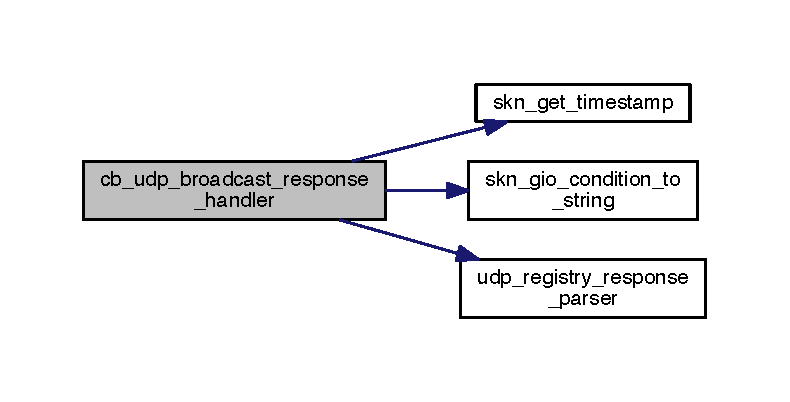
\includegraphics[width=350pt]{cmd_d_c_8c_a385b710fd30ba190b3b96e814424ff80_cgraph}
\end{center}
\end{figure}




Here is the caller graph for this function\+:
\nopagebreak
\begin{figure}[H]
\begin{center}
\leavevmode
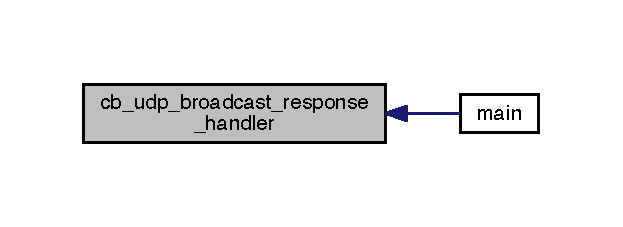
\includegraphics[width=299pt]{cmd_d_c_8c_a385b710fd30ba190b3b96e814424ff80_icgraph}
\end{center}
\end{figure}


\hypertarget{cmd_d_c_8c_a00c5b52bdcb7caec07d08b05b8c1dced}{}\index{cmd\+D\+C.\+c@{cmd\+D\+C.\+c}!cb\+\_\+udp\+\_\+comm\+\_\+request\+\_\+handler@{cb\+\_\+udp\+\_\+comm\+\_\+request\+\_\+handler}}
\index{cb\+\_\+udp\+\_\+comm\+\_\+request\+\_\+handler@{cb\+\_\+udp\+\_\+comm\+\_\+request\+\_\+handler}!cmd\+D\+C.\+c@{cmd\+D\+C.\+c}}
\subsubsection[{cb\+\_\+udp\+\_\+comm\+\_\+request\+\_\+handler(\+P\+Control\+Data pctrl)}]{\setlength{\rightskip}{0pt plus 5cm}static gboolean cb\+\_\+udp\+\_\+comm\+\_\+request\+\_\+handler (
\begin{DoxyParamCaption}
\item[{{\bf P\+Control\+Data}}]{pctrl}
\end{DoxyParamCaption}
)\hspace{0.3cm}{\ttfamily [static]}}\label{cmd_d_c_8c_a00c5b52bdcb7caec07d08b05b8c1dced}


Definition at line 526 of file cmd\+D\+C.\+c.



References \+\_\+control\+Data\+::ch\+\_\+display\+\_\+service\+\_\+name, \+\_\+control\+Data\+::ch\+\_\+message, \+\_\+control\+Data\+::g\+Error\+Count, \+\_\+control\+Data\+::gs\+D\+S\+Addr, \+\_\+control\+Data\+::g\+Sock, and \+\_\+control\+Data\+::loop.



Referenced by udp\+\_\+initialize\+\_\+message\+\_\+send().


\begin{DoxyCode}
526                                                                 \{
527     GError *error = NULL;
528 
529     \textcolor{keywordflow}{if} ( NULL == pctrl) \{  \textcolor{comment}{/* SHUTDOWN THE MAIN LOOP */}
530         g\_message(\textcolor{stringliteral}{"DisplayClient::cb\_udp\_comm\_request\_handler(error) Invalid Pointer"});
531         \textcolor{keywordflow}{return} ( G\_SOURCE\_REMOVE );
532     \}
533 
534     g\_socket\_send\_to (pctrl->\hyperlink{struct__control_data_a49b267275036fc3ac9b7d9e53b0625e1}{gSock}, pctrl->\hyperlink{struct__control_data_a11c618822b208569a5d28206407326d5}{gsDSAddr}, pctrl->
      \hyperlink{struct__control_data_a16162d5fe851704d7ea50ff16525b94c}{ch\_message}, strlen(pctrl->\hyperlink{struct__control_data_a16162d5fe851704d7ea50ff16525b94c}{ch\_message}), NULL, &error);
535     \textcolor{keywordflow}{if} (error != NULL) \{  \textcolor{comment}{// gss\_send = Number of bytes written (which may be less than size ), or -1 on
       error}
536         g\_error(\textcolor{stringliteral}{"g\_socket\_send\_to() => %s"}, error->message);
537         g\_clear\_error(&error);
538         pctrl->\hyperlink{struct__control_data_a0dcc9f369186f6cf7c99b2178be66e58}{gErrorCount} += 1;
539         \textcolor{keywordflow}{if}(pctrl->\hyperlink{struct__control_data_a0dcc9f369186f6cf7c99b2178be66e58}{gErrorCount} > 10) \{
540             g\_message(\textcolor{stringliteral}{"DisplayClient::cb\_udp\_comm\_request\_handler(error) Display Service @ %s, Not
       Responding!"}, pctrl->\hyperlink{struct__control_data_a94aa04264eafaa65a7a869a540bbdf93}{ch\_display\_service\_name});
541             g\_main\_loop\_quit(pctrl->\hyperlink{struct__control_data_ae1b70bafbd5eb568c6ca339664959216}{loop});
542             \textcolor{keywordflow}{return} ( G\_SOURCE\_REMOVE );
543         \} \textcolor{keywordflow}{else} \{
544             \textcolor{keywordflow}{return} (G\_SOURCE\_CONTINUE);
545         \}
546     \}
547 
548     g\_print(\textcolor{stringliteral}{"%s\(\backslash\)n"}, pctrl->\hyperlink{struct__control_data_a16162d5fe851704d7ea50ff16525b94c}{ch\_message}); \textcolor{comment}{// Todo not needed}
549 
550     \textcolor{keywordflow}{return} (G\_SOURCE\_CONTINUE);
551 \}
\end{DoxyCode}


Here is the caller graph for this function\+:
\nopagebreak
\begin{figure}[H]
\begin{center}
\leavevmode
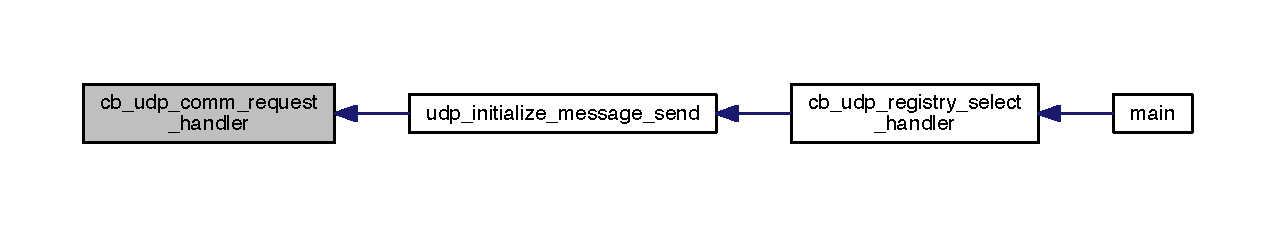
\includegraphics[width=350pt]{cmd_d_c_8c_a00c5b52bdcb7caec07d08b05b8c1dced_icgraph}
\end{center}
\end{figure}


\hypertarget{cmd_d_c_8c_aa8a19e68e54683fa324bcee1ecfd3942}{}\index{cmd\+D\+C.\+c@{cmd\+D\+C.\+c}!cb\+\_\+udp\+\_\+comm\+\_\+response\+\_\+handler@{cb\+\_\+udp\+\_\+comm\+\_\+response\+\_\+handler}}
\index{cb\+\_\+udp\+\_\+comm\+\_\+response\+\_\+handler@{cb\+\_\+udp\+\_\+comm\+\_\+response\+\_\+handler}!cmd\+D\+C.\+c@{cmd\+D\+C.\+c}}
\subsubsection[{cb\+\_\+udp\+\_\+comm\+\_\+response\+\_\+handler(\+G\+Socket $\ast$g\+Sock, G\+I\+O\+Condition condition, P\+Control\+Data pctrl)}]{\setlength{\rightskip}{0pt plus 5cm}static gboolean cb\+\_\+udp\+\_\+comm\+\_\+response\+\_\+handler (
\begin{DoxyParamCaption}
\item[{G\+Socket $\ast$}]{g\+Sock, }
\item[{G\+I\+O\+Condition}]{condition, }
\item[{{\bf P\+Control\+Data}}]{pctrl}
\end{DoxyParamCaption}
)\hspace{0.3cm}{\ttfamily [static]}}\label{cmd_d_c_8c_aa8a19e68e54683fa324bcee1ecfd3942}


Definition at line 468 of file cmd\+D\+C.\+c.



References \+\_\+control\+Data\+::ch\+\_\+request, \+\_\+control\+Data\+::ch\+\_\+response, \+\_\+control\+Data\+::g\+Error\+Count, \+\_\+control\+Data\+::resolver, and skn\+\_\+get\+\_\+timestamp().



Referenced by udp\+\_\+initialize\+\_\+message\+\_\+send().


\begin{DoxyCode}
468                                                                                                          \{
469     GError *error = NULL;
470     gssize gss\_receive = 0;
471     gchar *stamp = \hyperlink{cmd_d_c_8c_a8288aea959581188e5bd29430935a6ed}{skn\_get\_timestamp}();
472     gchar * rmtHost = NULL;
473     GSocketAddress *gsRmtAddr = NULL;
474     GInetAddress *gsAddr = NULL;
475     gchar *converted = NULL;
476 
477     \textcolor{keywordflow}{if} ( NULL == pctrl) \{  \textcolor{comment}{/* SHUTDOWN THE MAIN LOOP */}
478         g\_message(\textcolor{stringliteral}{"DisplayClient::cb\_udp\_comm\_response\_handler(error) Invalid Pointer"});
479         \textcolor{keywordflow}{return} ( G\_SOURCE\_REMOVE );
480     \}
481 
482     gss\_receive = g\_socket\_receive\_from(gSock, &gsRmtAddr, pctrl->\hyperlink{struct__control_data_a948c37bbe26f5bdd4841b65384155edf}{ch\_request}, \textcolor{keyword}{sizeof}(pctrl->
      \hyperlink{struct__control_data_a948c37bbe26f5bdd4841b65384155edf}{ch\_request}), NULL, &error);
483     \textcolor{keywordflow}{if} (error != NULL) \{ \textcolor{comment}{// gss\_receive = Number of bytes read, or 0 if the connection was closed by the
       peer, or -1 on error}
484         g\_error(\textcolor{stringliteral}{"g\_socket\_receive() => %s"}, error->message);
485         g\_clear\_error(&error);
486     \}
487     \textcolor{keywordflow}{if} (gss\_receive > 0 ) \{
488         pctrl->\hyperlink{struct__control_data_a948c37bbe26f5bdd4841b65384155edf}{ch\_request}[gss\_receive] = 0;
489         \textcolor{keywordflow}{if} (G\_IS\_INET\_SOCKET\_ADDRESS(gsRmtAddr) ) \{
490             gsAddr = g\_inet\_socket\_address\_get\_address( G\_INET\_SOCKET\_ADDRESS(gsRmtAddr) );
491             \textcolor{keywordflow}{if} ( G\_IS\_INET\_ADDRESS(gsAddr) ) \{
492                 g\_object\_ref(gsAddr);
493                 rmtHost = g\_resolver\_lookup\_by\_address (pctrl->\hyperlink{struct__control_data_afe33a7083e1ecc9ba50a69644ed4a753}{resolver}, gsAddr, NULL, NULL);
494                 \textcolor{keywordflow}{if} (NULL == rmtHost) \{
495                     rmtHost = g\_inet\_address\_to\_string ( gsAddr);
496                 \}
497             \}
498         \}
499 
500         \textcolor{comment}{/*}
501 \textcolor{comment}{         * Convert to UTF8 */}
502         converted = g\_convert (pctrl->\hyperlink{struct__control_data_a948c37bbe26f5bdd4841b65384155edf}{ch\_request}, gss\_receive, \textcolor{stringliteral}{"UTF-8"}, \textcolor{stringliteral}{"ISO-8859-1"}, NULL, NULL,
       NULL);
503         \textcolor{keywordflow}{if} (NULL != converted) \{
504             g\_utf8\_strncpy(pctrl->\hyperlink{struct__control_data_a948c37bbe26f5bdd4841b65384155edf}{ch\_request}, converted, \textcolor{keyword}{sizeof}(pctrl->
      \hyperlink{struct__control_data_a948c37bbe26f5bdd4841b65384155edf}{ch\_request}));
505             g\_free(converted);
506         \}
507 
508         g\_snprintf(pctrl->\hyperlink{struct__control_data_a9423e8582b05e2dde58b7302bee5559b}{ch\_response}, \textcolor{keyword}{sizeof}(pctrl->\hyperlink{struct__control_data_a9423e8582b05e2dde58b7302bee5559b}{ch\_response}), \textcolor{stringliteral}{"[%s]RESPONSE
       From=%s, Msg=%s"}, stamp, rmtHost, pctrl->\hyperlink{struct__control_data_a948c37bbe26f5bdd4841b65384155edf}{ch\_request});
509         pctrl->\hyperlink{struct__control_data_a0dcc9f369186f6cf7c99b2178be66e58}{gErrorCount} = 0;  \textcolor{comment}{// reset send errors}
510     \} \textcolor{keywordflow}{else} \{
511         g\_snprintf(pctrl->\hyperlink{struct__control_data_a9423e8582b05e2dde58b7302bee5559b}{ch\_response}, \textcolor{keyword}{sizeof}(pctrl->\hyperlink{struct__control_data_a9423e8582b05e2dde58b7302bee5559b}{ch\_response}), \textcolor{stringliteral}{"%s"}, \textcolor{stringliteral}{"Error:
       Input not Usable!"});
512     \}
513 
514     g\_print(\textcolor{stringliteral}{"%s\(\backslash\)n"}, pctrl->\hyperlink{struct__control_data_a9423e8582b05e2dde58b7302bee5559b}{ch\_response});
515     g\_free(stamp);
516 
517     \textcolor{keywordflow}{if} ( G\_IS\_INET\_ADDRESS(gsAddr) )
518         g\_object\_unref(gsAddr);
519 
520     \textcolor{keywordflow}{if} ( G\_IS\_INET\_SOCKET\_ADDRESS(gsRmtAddr) )
521         g\_object\_unref(gsRmtAddr);
522 
523     \textcolor{keywordflow}{return} (G\_SOURCE\_CONTINUE);
524 \}
\end{DoxyCode}


Here is the call graph for this function\+:
\nopagebreak
\begin{figure}[H]
\begin{center}
\leavevmode
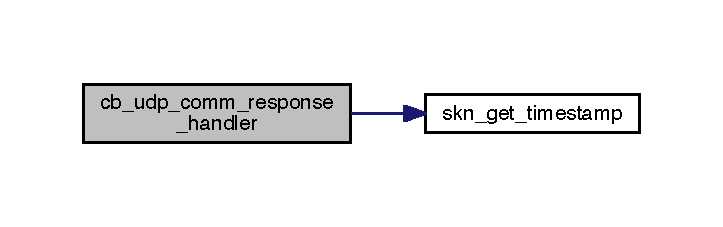
\includegraphics[width=347pt]{cmd_d_c_8c_aa8a19e68e54683fa324bcee1ecfd3942_cgraph}
\end{center}
\end{figure}




Here is the caller graph for this function\+:
\nopagebreak
\begin{figure}[H]
\begin{center}
\leavevmode
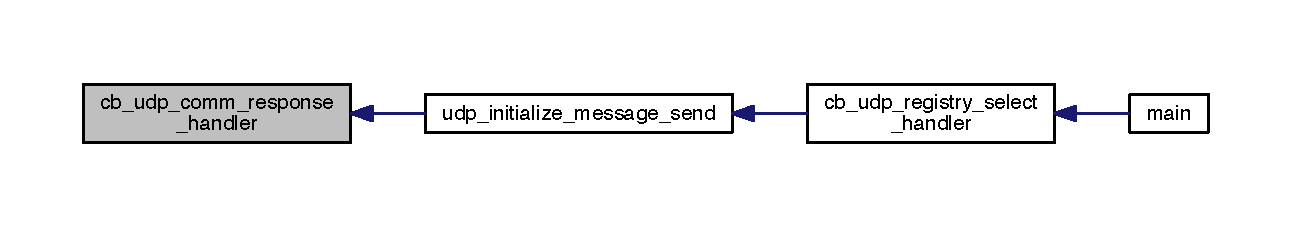
\includegraphics[width=350pt]{cmd_d_c_8c_aa8a19e68e54683fa324bcee1ecfd3942_icgraph}
\end{center}
\end{figure}


\hypertarget{cmd_d_c_8c_a160bb2056d3842ef84fd7211ed6ec385}{}\index{cmd\+D\+C.\+c@{cmd\+D\+C.\+c}!cb\+\_\+udp\+\_\+registry\+\_\+select\+\_\+handler@{cb\+\_\+udp\+\_\+registry\+\_\+select\+\_\+handler}}
\index{cb\+\_\+udp\+\_\+registry\+\_\+select\+\_\+handler@{cb\+\_\+udp\+\_\+registry\+\_\+select\+\_\+handler}!cmd\+D\+C.\+c@{cmd\+D\+C.\+c}}
\subsubsection[{cb\+\_\+udp\+\_\+registry\+\_\+select\+\_\+handler(\+P\+Control\+Data pctrl)}]{\setlength{\rightskip}{0pt plus 5cm}static gboolean cb\+\_\+udp\+\_\+registry\+\_\+select\+\_\+handler (
\begin{DoxyParamCaption}
\item[{{\bf P\+Control\+Data}}]{pctrl}
\end{DoxyParamCaption}
)\hspace{0.3cm}{\ttfamily [static]}}\label{cmd_d_c_8c_a160bb2056d3842ef84fd7211ed6ec385}


Definition at line 689 of file cmd\+D\+C.\+c.



References \+\_\+control\+Data\+::ch\+\_\+display\+\_\+service\+\_\+name, \+\_\+registry\+Data\+::ch\+\_\+ip, \+\_\+registry\+Data\+::ch\+\_\+name, \+\_\+registry\+Data\+::ch\+\_\+port, \+\_\+control\+Data\+::g\+Broadcast\+Socket, \+\_\+control\+Data\+::gl\+Registry, \+\_\+control\+Data\+::g\+Msg\+Delay, \+\_\+control\+Data\+::g\+Ready, \+\_\+control\+Data\+::g\+Registry\+Queries, \+\_\+control\+Data\+::gs\+D\+S\+Addr, \+\_\+control\+Data\+::pa\+B, skn\+\_\+udp\+\_\+network\+\_\+broadcast\+\_\+all\+\_\+interfaces(), udp\+\_\+initialize\+\_\+message\+\_\+send(), and udp\+\_\+registry\+\_\+find\+\_\+by\+\_\+name().



Referenced by main().


\begin{DoxyCode}
689                                                                    \{
690     GList *registry = NULL;
691     \hyperlink{struct__registry_data}{PRegData} preg = NULL;
692     GInetAddress *anyAddr = NULL;
693 
694     g\_return\_val\_if\_fail((NULL != pctrl), G\_SOURCE\_REMOVE);
695 
696     \textcolor{comment}{/*}
697 \textcolor{comment}{     * Find in Registry the selected service name */}
698     \textcolor{keywordflow}{if} (g\_list\_length(pctrl->\hyperlink{struct__control_data_a34b1729bc0b37c9dce0327ea4cd8a812}{glRegistry}) < 1) \{
699         pctrl->\hyperlink{struct__control_data_ab4837eb7cc16bf85fe0bd839a428eaa5}{gRegistryQueries}++;
700 
701         \textcolor{keywordflow}{if} ((pctrl->\hyperlink{struct__control_data_ab4837eb7cc16bf85fe0bd839a428eaa5}{gRegistryQueries} % 15) == 0) \{  \textcolor{comment}{// every 30 seconds redo query}
702             g\_print(\textcolor{stringliteral}{"[REGISTRY] Looking for [%s] in Rpi Registry every 30 seconds.  StandBy...\(\backslash\)n"}, pctrl->
      \hyperlink{struct__control_data_a94aa04264eafaa65a7a869a540bbdf93}{ch\_display\_service\_name});
703             \hyperlink{cmd_d_c_8c_af376243f65a3fd761050836d1293b0d9}{skn\_udp\_network\_broadcast\_all\_interfaces}(pctrl->
      \hyperlink{struct__control_data_a05fab30fce92ebe541d9dd98220c60ef}{gBroadcastSocket}, pctrl->\hyperlink{struct__control_data_a93f6e099a56c0d476607b4bd5a9dfa58}{paB});
704         \}
705 
706         \textcolor{keywordflow}{return} (G\_SOURCE\_CONTINUE);
707     \}
708 
709     \textcolor{keywordflow}{if} ( NULL == (registry = g\_list\_find\_custom (pctrl->\hyperlink{struct__control_data_a34b1729bc0b37c9dce0327ea4cd8a812}{glRegistry}, pctrl->
      \hyperlink{struct__control_data_a94aa04264eafaa65a7a869a540bbdf93}{ch\_display\_service\_name}, (GCompareFunc)
      \hyperlink{cmd_d_c_8c_ae59da66ef51690f71da087514886fd12}{udp\_registry\_find\_by\_name})) ) \{
710         \textcolor{keywordflow}{return} (G\_SOURCE\_CONTINUE);
711     \}
712 
713     preg = registry->data; \textcolor{comment}{// now extract ip and port}
714     \textcolor{comment}{/* Display Service Address */}
715 
716     anyAddr = g\_inet\_address\_new\_from\_string(preg->\hyperlink{struct__registry_data_a814e064e77a6aac5866c88cb51acd971}{ch\_ip}); \textcolor{comment}{// g\_object\_unref(dIP) when done}
717     \textcolor{keywordflow}{if} (NULL == anyAddr) \{
718         g\_error(\textcolor{stringliteral}{"g\_inet\_address\_new\_from\_string() Failed => %s, %s"}, preg->
      \hyperlink{struct__registry_data_a4764e2a72c3ba9177b6c4803cfa03f72}{ch\_name}, preg->\hyperlink{struct__registry_data_a814e064e77a6aac5866c88cb51acd971}{ch\_ip});
719         \textcolor{keywordflow}{return}(G\_SOURCE\_CONTINUE);
720     \}
721     pctrl->\hyperlink{struct__control_data_a11c618822b208569a5d28206407326d5}{gsDSAddr} = g\_inet\_socket\_address\_new(anyAddr,  g\_ascii\_strtoll(preg->
      \hyperlink{struct__registry_data_a74f03616af9ec9770266cb7988fe1a71}{ch\_port}, NULL, 10));
722         g\_object\_unref(anyAddr);
723 
724     pctrl->\hyperlink{struct__control_data_a04238362a20b6616913d869fc464e4b2}{gReady} = \hyperlink{cmd_d_c_8c_a793c6b3e5c7a5abc993d8cfbe963629d}{udp\_initialize\_message\_send}(pctrl);
725 
726     \textcolor{keywordflow}{if} (pctrl->\hyperlink{struct__control_data_a04238362a20b6616913d869fc464e4b2}{gReady}) \{
727         g\_print(\textcolor{stringliteral}{"[REGISTRY] FOUND %s on ip %s:%s, sending your message %d seconds.\(\backslash\)n\(\backslash\)n"}, preg->
      \hyperlink{struct__registry_data_a4764e2a72c3ba9177b6c4803cfa03f72}{ch\_name}, preg->\hyperlink{struct__registry_data_a814e064e77a6aac5866c88cb51acd971}{ch\_ip}, preg->\hyperlink{struct__registry_data_a74f03616af9ec9770266cb7988fe1a71}{ch\_port}, pctrl->\hyperlink{struct__control_data_a277ea878a8491fa38269b6c762a05389}{gMsgDelay});
728         \textcolor{keywordflow}{return} (G\_SOURCE\_REMOVE);
729     \} \textcolor{keywordflow}{else} \{
730         \textcolor{keywordflow}{return} (G\_SOURCE\_CONTINUE);
731     \}
732 \}
\end{DoxyCode}


Here is the call graph for this function\+:
\nopagebreak
\begin{figure}[H]
\begin{center}
\leavevmode
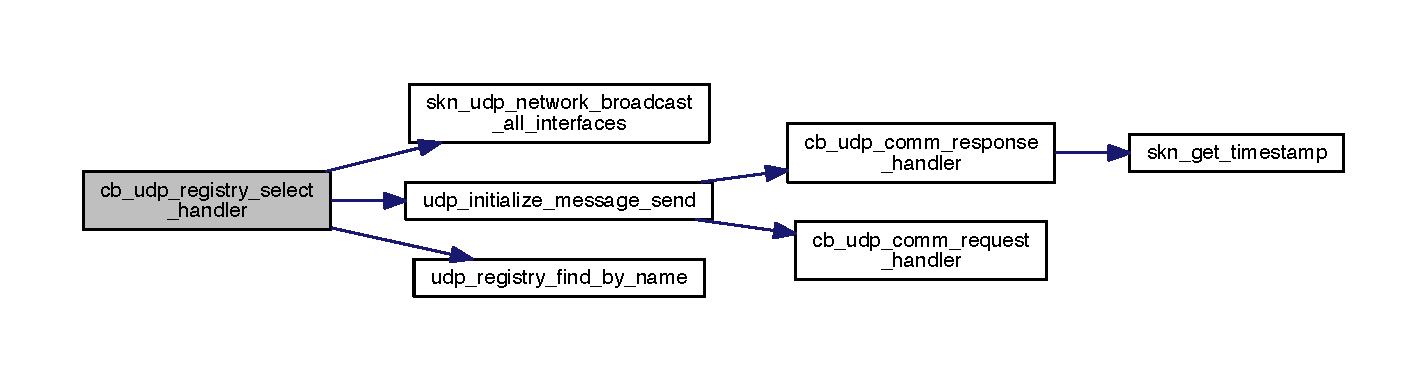
\includegraphics[width=350pt]{cmd_d_c_8c_a160bb2056d3842ef84fd7211ed6ec385_cgraph}
\end{center}
\end{figure}




Here is the caller graph for this function\+:
\nopagebreak
\begin{figure}[H]
\begin{center}
\leavevmode
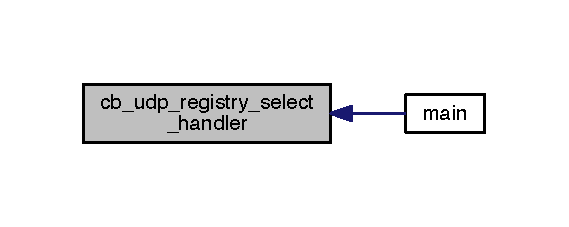
\includegraphics[width=273pt]{cmd_d_c_8c_a160bb2056d3842ef84fd7211ed6ec385_icgraph}
\end{center}
\end{figure}


\hypertarget{cmd_d_c_8c_a76ad4de5945cff6e20dbeff46bda868b}{}\index{cmd\+D\+C.\+c@{cmd\+D\+C.\+c}!cb\+\_\+unix\+\_\+signal\+\_\+handler@{cb\+\_\+unix\+\_\+signal\+\_\+handler}}
\index{cb\+\_\+unix\+\_\+signal\+\_\+handler@{cb\+\_\+unix\+\_\+signal\+\_\+handler}!cmd\+D\+C.\+c@{cmd\+D\+C.\+c}}
\subsubsection[{cb\+\_\+unix\+\_\+signal\+\_\+handler(\+P\+U\+Signal\+Data psig)}]{\setlength{\rightskip}{0pt plus 5cm}static gboolean cb\+\_\+unix\+\_\+signal\+\_\+handler (
\begin{DoxyParamCaption}
\item[{{\bf P\+U\+Signal\+Data}}]{psig}
\end{DoxyParamCaption}
)\hspace{0.3cm}{\ttfamily [static]}}\label{cmd_d_c_8c_a76ad4de5945cff6e20dbeff46bda868b}


Definition at line 734 of file cmd\+D\+C.\+c.



References \+\_\+signal\+Data\+::loop, and \+\_\+signal\+Data\+::signal\+Name.



Referenced by main().


\begin{DoxyCode}
734                                                           \{
735     g\_message(\textcolor{stringliteral}{"DisplayClient::cb\_unix\_signal\_handler() %s Unix Signal Received => Shutdown Initiated!\(\backslash\)n"}, 
      psig->\hyperlink{struct__signal_data_a6b2ce59a22a4ccc54e1d7a54e641d08f}{signalName});
736     g\_main\_loop\_quit(psig->\hyperlink{struct__signal_data_ae85864980ae30c1878e7149c26442544}{loop});
737     \textcolor{keywordflow}{return} ( G\_SOURCE\_REMOVE );
738 \}
\end{DoxyCode}


Here is the caller graph for this function\+:
\nopagebreak
\begin{figure}[H]
\begin{center}
\leavevmode
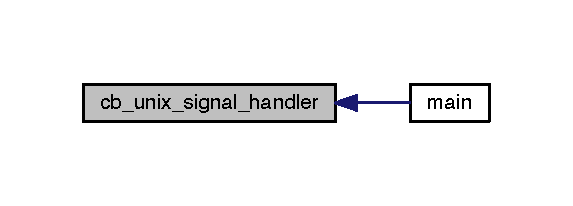
\includegraphics[width=275pt]{cmd_d_c_8c_a76ad4de5945cff6e20dbeff46bda868b_icgraph}
\end{center}
\end{figure}


\hypertarget{cmd_d_c_8c_a3c04138a5bfe5d72780bb7e82a18e627}{}\index{cmd\+D\+C.\+c@{cmd\+D\+C.\+c}!main@{main}}
\index{main@{main}!cmd\+D\+C.\+c@{cmd\+D\+C.\+c}}
\subsubsection[{main(int argc, char $\ast$$\ast$argv)}]{\setlength{\rightskip}{0pt plus 5cm}int main (
\begin{DoxyParamCaption}
\item[{int}]{argc, }
\item[{char $\ast$$\ast$}]{argv}
\end{DoxyParamCaption}
)}\label{cmd_d_c_8c_a3c04138a5bfe5d72780bb7e82a18e627}


Definition at line 740 of file cmd\+D\+C.\+c.



References cb\+\_\+udp\+\_\+broadcast\+\_\+response\+\_\+handler(), cb\+\_\+udp\+\_\+registry\+\_\+select\+\_\+handler(), cb\+\_\+unix\+\_\+signal\+\_\+handler(), \+\_\+control\+Data\+::ch\+\_\+display\+\_\+service\+\_\+name, \+\_\+control\+Data\+::ch\+\_\+intf\+Name, \+\_\+control\+Data\+::ch\+\_\+message, \+\_\+control\+Data\+::ch\+\_\+this\+\_\+ip, F\+A\+L\+S\+E, G\+\_\+\+O\+P\+T\+I\+O\+N\+\_\+\+F\+L\+A\+G\+\_\+\+N\+O\+N\+E, \+\_\+control\+Data\+::g\+Broadcast\+Socket, \+\_\+control\+Data\+::g\+Comm\+Source, \+\_\+control\+Data\+::g\+Error\+Count, \+\_\+control\+Data\+::gl\+Registry, \+\_\+control\+Data\+::g\+Msg\+Delay, \+\_\+control\+Data\+::g\+Ready, \+\_\+control\+Data\+::g\+Reg\+Count, \+\_\+control\+Data\+::g\+Registry\+Queries, \+\_\+control\+Data\+::gs\+Addr, \+\_\+control\+Data\+::gs\+D\+S\+Addr, \+\_\+control\+Data\+::g\+Sock, \+\_\+signal\+Data\+::loop, \+\_\+control\+Data\+::loop, M\+S\+G\+\_\+\+D\+E\+L\+A\+Y\+\_\+\+I\+N\+T\+E\+R\+V\+A\+L, \+\_\+control\+Data\+::pa\+B, \+\_\+control\+Data\+::resolver, \+\_\+control\+Data\+::sig\+Hup, \+\_\+control\+Data\+::sig\+Int, \+\_\+signal\+Data\+::signal\+Name, \+\_\+control\+Data\+::sig\+Term, skn\+\_\+get\+\_\+default\+\_\+interface\+\_\+name\+\_\+and\+\_\+ipv4\+\_\+address(), S\+K\+N\+\_\+\+U\+D\+P\+\_\+\+A\+N\+Y\+\_\+\+P\+O\+R\+T, skn\+\_\+udp\+\_\+network\+\_\+broadcast\+\_\+all\+\_\+interfaces(), and T\+R\+U\+E.


\begin{DoxyCode}
740                                 \{
741 
742     \hyperlink{struct__control_data}{ControlData} cData;
743     GSource * gBroadSource = NULL;
744     GError *error = NULL;
745     GSocket *gSock;
746     GSocketAddress *gsAddr = NULL;
747     GInetAddress *anyAddr = NULL;
748 
749     gchar * pch\_display\_service\_name = NULL;
750     gchar * pch\_message = NULL;
751 
752     cData.\hyperlink{struct__control_data_a277ea878a8491fa38269b6c762a05389}{gMsgDelay} = \hyperlink{cmd_d_c_8c_ac66d92e429586a7c5d0424fe6ad105dd}{MSG\_DELAY\_INTERVAL};
753     cData.\hyperlink{struct__control_data_a0dcc9f369186f6cf7c99b2178be66e58}{gErrorCount} = 0;
754     cData.\hyperlink{struct__control_data_a81bfc0d50c23ebe6708e065659d11eb8}{gRegCount} = 0;
755     cData.\hyperlink{struct__control_data_ab4837eb7cc16bf85fe0bd839a428eaa5}{gRegistryQueries} = 0;
756     cData.\hyperlink{struct__control_data_a04238362a20b6616913d869fc464e4b2}{gReady} = \hyperlink{skn__common__headers_8h_aa93f0eb578d23995850d61f7d61c55c1}{FALSE};
757 
758     cData.\hyperlink{struct__control_data_a34b1729bc0b37c9dce0327ea4cd8a812}{glRegistry} = NULL;
759     cData.\hyperlink{struct__control_data_af45dc1f0c4806eaac0a57da17db50fdb}{sigTerm}.\hyperlink{struct__signal_data_a6b2ce59a22a4ccc54e1d7a54e641d08f}{signalName} = \textcolor{stringliteral}{"SIGTERM"};
760     cData.\hyperlink{struct__control_data_ae8ad5b5af46f4ab4bcd6ffb41e83385b}{sigInt}.\hyperlink{struct__signal_data_a6b2ce59a22a4ccc54e1d7a54e641d08f}{signalName} = \textcolor{stringliteral}{"SIGINT"};
761     cData.\hyperlink{struct__control_data_a551d0ecd4ceb9fc4ce8eebe5a984dc4c}{sigHup}.\hyperlink{struct__signal_data_a6b2ce59a22a4ccc54e1d7a54e641d08f}{signalName} = \textcolor{stringliteral}{"SIGHUP"};
762     cData.\hyperlink{struct__control_data_a0dcc9f369186f6cf7c99b2178be66e58}{gErrorCount} = 0;
763     cData.\hyperlink{struct__control_data_afe33a7083e1ecc9ba50a69644ed4a753}{resolver} = g\_resolver\_get\_default();
764 
765     GOptionContext *gOptions = NULL;
766     GOptionEntry pgmOptions[] = \{
767        \{\textcolor{stringliteral}{"display\_service\_name"}, \textcolor{charliteral}{'a'}, \hyperlink{cmd_d_c_8c_a8e8475ded7103e72515667b568ed64c7}{G\_OPTION\_FLAG\_NONE}, G\_OPTION\_ARG\_STRING, &
      pch\_display\_service\_name, \textcolor{stringliteral}{"DisplayService Name"}, \textcolor{stringliteral}{"gtk\_display\_service"}\},
768        \{\textcolor{stringliteral}{"display\_message"}, \textcolor{charliteral}{'m'}, \hyperlink{cmd_d_c_8c_a8e8475ded7103e72515667b568ed64c7}{G\_OPTION\_FLAG\_NONE}, G\_OPTION\_ARG\_STRING, &pch\_message, \textcolor{stringliteral}{"
      Message to send to DisplayService"}, \textcolor{stringliteral}{"single-quoted-string"}\},
769        \{\textcolor{stringliteral}{"message\_interval\_delay"}, \textcolor{charliteral}{'n'}, \hyperlink{cmd_d_c_8c_a8e8475ded7103e72515667b568ed64c7}{G\_OPTION\_FLAG\_NONE}, G\_OPTION\_ARG\_INT, &cData.
      \hyperlink{struct__control_data_a277ea878a8491fa38269b6c762a05389}{gMsgDelay}, \textcolor{stringliteral}{"Send one message every Interval."}, \textcolor{stringliteral}{"[1 to 300] seconds, default no-repeat"}\},
770        \{NULL\}
771     \};
772 
773     gOptions = g\_option\_context\_new (\textcolor{stringliteral}{"UDP message display client for IOT."});
774     g\_option\_context\_add\_main\_entries (gOptions, pgmOptions, NULL);
775     g\_option\_context\_parse (gOptions, &argc, &argv, &error);
776     \textcolor{keywordflow}{if} (error != NULL) \{
777         g\_error(\textcolor{stringliteral}{"g\_option\_context\_parse() => %s"}, error->message);
778         g\_clear\_error(&error);
779         exit(EXIT\_FAILURE);
780     \}
781     g\_option\_context\_free(gOptions);
782 
783     \textcolor{keywordflow}{if} (NULL == pch\_message) \{
784         g\_utf8\_strncpy(cData.\hyperlink{struct__control_data_a16162d5fe851704d7ea50ff16525b94c}{ch\_message}, \textcolor{stringliteral}{"GTK-+3.0 Rocks with GLIB-2.0 on any platform! (cldc)"}, \textcolor{keyword}{
      sizeof}(cData.\hyperlink{struct__control_data_a16162d5fe851704d7ea50ff16525b94c}{ch\_message}));
785     \} \textcolor{keywordflow}{else} \{
786         g\_utf8\_strncpy(cData.\hyperlink{struct__control_data_a16162d5fe851704d7ea50ff16525b94c}{ch\_message}, pch\_message, \textcolor{keyword}{sizeof}(cData.
      \hyperlink{struct__control_data_a16162d5fe851704d7ea50ff16525b94c}{ch\_message}));
787         g\_free(pch\_message);
788     \}
789     \textcolor{keywordflow}{if} (NULL == pch\_display\_service\_name) \{
790         g\_utf8\_strncpy(cData.\hyperlink{struct__control_data_a94aa04264eafaa65a7a869a540bbdf93}{ch\_display\_service\_name}, \textcolor{stringliteral}{"gtk\_display\_service"}, \textcolor{keyword}{sizeof}(
      cData.\hyperlink{struct__control_data_a94aa04264eafaa65a7a869a540bbdf93}{ch\_display\_service\_name}));
791     \} \textcolor{keywordflow}{else} \{
792         g\_utf8\_strncpy(cData.\hyperlink{struct__control_data_a94aa04264eafaa65a7a869a540bbdf93}{ch\_display\_service\_name}, pch\_display\_service\_name, \textcolor{keyword}{
      sizeof}(cData.\hyperlink{struct__control_data_a94aa04264eafaa65a7a869a540bbdf93}{ch\_display\_service\_name}));
793         g\_free(pch\_display\_service\_name);
794     \}
795     \textcolor{keywordflow}{if} (0 == cData.\hyperlink{struct__control_data_a277ea878a8491fa38269b6c762a05389}{gMsgDelay}) \{
796         cData.\hyperlink{struct__control_data_a277ea878a8491fa38269b6c762a05389}{gMsgDelay} = \hyperlink{cmd_d_c_8c_ac66d92e429586a7c5d0424fe6ad105dd}{MSG\_DELAY\_INTERVAL};
797     \}
798 
799     cData.\hyperlink{struct__control_data_a93f6e099a56c0d476607b4bd5a9dfa58}{paB} = NULL;
800     cData.\hyperlink{struct__control_data_a93f6e099a56c0d476607b4bd5a9dfa58}{paB} = \hyperlink{cmd_d_c_8c_a72be87baa67e532c78af054acf935d6c}{skn\_get\_default\_interface\_name\_and\_ipv4\_address}
      ((\textcolor{keywordtype}{char} *)&cData.\hyperlink{struct__control_data_adac6cf5482e4bbabb442f8ab27e4bc62}{ch\_intfName}, (\textcolor{keywordtype}{char} *)&cData.\hyperlink{struct__control_data_ac48fc4263dd4a6bad484b93fbf1ffe1b}{ch\_this\_ip});
801     \textcolor{keywordflow}{if} (NULL == cData.\hyperlink{struct__control_data_a93f6e099a56c0d476607b4bd5a9dfa58}{paB}) \{
802         g\_error(\textcolor{stringliteral}{"skn\_skn\_get\_default\_interface\_name\_and\_ipv4\_address() => Unable to discover network
       interface or non-available."});
803         exit(EXIT\_FAILURE);
804     \}
805 
806     cData.\hyperlink{struct__control_data_a551d0ecd4ceb9fc4ce8eebe5a984dc4c}{sigHup}.\hyperlink{struct__signal_data_ae85864980ae30c1878e7149c26442544}{loop} = cData.\hyperlink{struct__control_data_af45dc1f0c4806eaac0a57da17db50fdb}{sigTerm}.\hyperlink{struct__signal_data_ae85864980ae30c1878e7149c26442544}{loop} = cData.\hyperlink{struct__control_data_ae8ad5b5af46f4ab4bcd6ffb41e83385b}{sigInt}.
      \hyperlink{struct__signal_data_ae85864980ae30c1878e7149c26442544}{loop} = cData.\hyperlink{struct__control_data_ae1b70bafbd5eb568c6ca339664959216}{loop} =  g\_main\_loop\_new(NULL, \hyperlink{skn__common__headers_8h_aa93f0eb578d23995850d61f7d61c55c1}{FALSE});
807 
808     \textcolor{comment}{/*}
809 \textcolor{comment}{     * Create broadcast UDP Socket for receiving messages */}
810     cData.\hyperlink{struct__control_data_a05fab30fce92ebe541d9dd98220c60ef}{gBroadcastSocket} = gSock = g\_socket\_new(G\_SOCKET\_FAMILY\_IPV4, 
      G\_SOCKET\_TYPE\_DATAGRAM, G\_SOCKET\_PROTOCOL\_UDP, &error);
811     \textcolor{keywordflow}{if} (error != NULL) \{
812         g\_error(\textcolor{stringliteral}{"g\_socket\_new(broadcast) => %s"}, error->message);
813         g\_clear\_error(&error);
814         exit(EXIT\_FAILURE);
815     \}
816     g\_socket\_set\_broadcast(gSock, \hyperlink{skn__common__headers_8h_aa8cecfc5c5c054d2875c03e77b7be15d}{TRUE});
817 
818     anyAddr = g\_inet\_address\_new\_any(G\_SOCKET\_FAMILY\_IPV4);
819     gsAddr  = g\_inet\_socket\_address\_new(anyAddr, \hyperlink{cmd_d_c_8c_a8091fbaa709d661a678a82a62fab638b}{SKN\_UDP\_ANY\_PORT});
820         g\_object\_unref(anyAddr);
821 
822     g\_socket\_bind(gSock, gsAddr, \hyperlink{skn__common__headers_8h_aa8cecfc5c5c054d2875c03e77b7be15d}{TRUE}, &error);
823     \textcolor{keywordflow}{if} (error != NULL) \{
824         g\_error(\textcolor{stringliteral}{"g\_socket\_bind() => %s"}, error->message);
825         g\_clear\_error(&error);
826         exit(EXIT\_FAILURE);
827     \}
828 
829     gBroadSource = g\_socket\_create\_source(gSock, G\_IO\_IN, NULL);
830         g\_source\_ref(gBroadSource);
831         g\_source\_set\_callback (gBroadSource, (GSourceFunc) 
      \hyperlink{cmd_d_c_8c_a385b710fd30ba190b3b96e814424ff80}{cb\_udp\_broadcast\_response\_handler}, &cData, NULL); \textcolor{comment}{// its really a
       GSocketSourceFunc}
832         g\_source\_attach (gBroadSource, NULL);
833 
834     \textcolor{comment}{/*}
835 \textcolor{comment}{     * Handle ctrl-break and kill signals cleanly */}
836     g\_unix\_signal\_add (SIGINT, (GSourceFunc) \hyperlink{cmd_d_c_8c_a76ad4de5945cff6e20dbeff46bda868b}{cb\_unix\_signal\_handler}, &cData.
      \hyperlink{struct__control_data_ae8ad5b5af46f4ab4bcd6ffb41e83385b}{sigInt}); \textcolor{comment}{// SIGINT signal (Ctrl+C)}
837     g\_unix\_signal\_add (SIGHUP, (GSourceFunc) \hyperlink{cmd_d_c_8c_a76ad4de5945cff6e20dbeff46bda868b}{cb\_unix\_signal\_handler}, &cData.
      \hyperlink{struct__control_data_a551d0ecd4ceb9fc4ce8eebe5a984dc4c}{sigHup});
838     g\_unix\_signal\_add (SIGTERM,(GSourceFunc) \hyperlink{cmd_d_c_8c_a76ad4de5945cff6e20dbeff46bda868b}{cb\_unix\_signal\_handler}, &cData.
      \hyperlink{struct__control_data_af45dc1f0c4806eaac0a57da17db50fdb}{sigTerm});
839 
840     \textcolor{comment}{/*}
841 \textcolor{comment}{     * Broadcast Registry Request: 10.100.1.255 */}
842     \textcolor{keywordflow}{if} ( \hyperlink{cmd_d_c_8c_af376243f65a3fd761050836d1293b0d9}{skn\_udp\_network\_broadcast\_all\_interfaces}(gSock, cData.
      \hyperlink{struct__control_data_a93f6e099a56c0d476607b4bd5a9dfa58}{paB}) ) \{
843         \textcolor{comment}{/*}
844 \textcolor{comment}{         * Setup 2secTimer to find display\_service before starting rest  */}
845         g\_timeout\_add (2000, (GSourceFunc)\hyperlink{cmd_d_c_8c_a160bb2056d3842ef84fd7211ed6ec385}{cb\_udp\_registry\_select\_handler}, &
      cData);
846 
847         g\_print(\textcolor{stringliteral}{"[REGISTRY] Looking for [%s] in Rpi Registry.  StandBy...\(\backslash\)n"}, cData.
      \hyperlink{struct__control_data_a94aa04264eafaa65a7a869a540bbdf93}{ch\_display\_service\_name});
848 
849         g\_main\_loop\_run(cData.\hyperlink{struct__control_data_ae1b70bafbd5eb568c6ca339664959216}{loop});
850     \}
851 
852     g\_main\_loop\_unref(cData.\hyperlink{struct__control_data_ae1b70bafbd5eb568c6ca339664959216}{loop});
853 
854     g\_source\_unref(gBroadSource);
855     g\_object\_unref(gSock);
856     g\_object\_unref(gsAddr);
857 
858     \textcolor{keywordflow}{if} (cData.\hyperlink{struct__control_data_a04238362a20b6616913d869fc464e4b2}{gReady}) \{
859         g\_source\_unref(cData.\hyperlink{struct__control_data_abfbd9e642ba240fa5985f63d60886de4}{gCommSource});
860         g\_object\_unref(cData.\hyperlink{struct__control_data_a49b267275036fc3ac9b7d9e53b0625e1}{gSock});
861         g\_object\_unref(cData.\hyperlink{struct__control_data_a11c618822b208569a5d28206407326d5}{gsDSAddr});
862         g\_object\_unref(cData.\hyperlink{struct__control_data_a8a43853386551af4c746fd4b882eb2bf}{gsAddr});
863     \}
864 
865     g\_free(cData.\hyperlink{struct__control_data_a93f6e099a56c0d476607b4bd5a9dfa58}{paB});
866     g\_list\_free\_full(cData.\hyperlink{struct__control_data_a34b1729bc0b37c9dce0327ea4cd8a812}{glRegistry}, (GDestroyNotify)g\_free);
867 
868     g\_message(\textcolor{stringliteral}{"cmdDC: normal shutdown..."});
869 
870     exit(EXIT\_SUCCESS);
871 \}
\end{DoxyCode}


Here is the call graph for this function\+:
\nopagebreak
\begin{figure}[H]
\begin{center}
\leavevmode
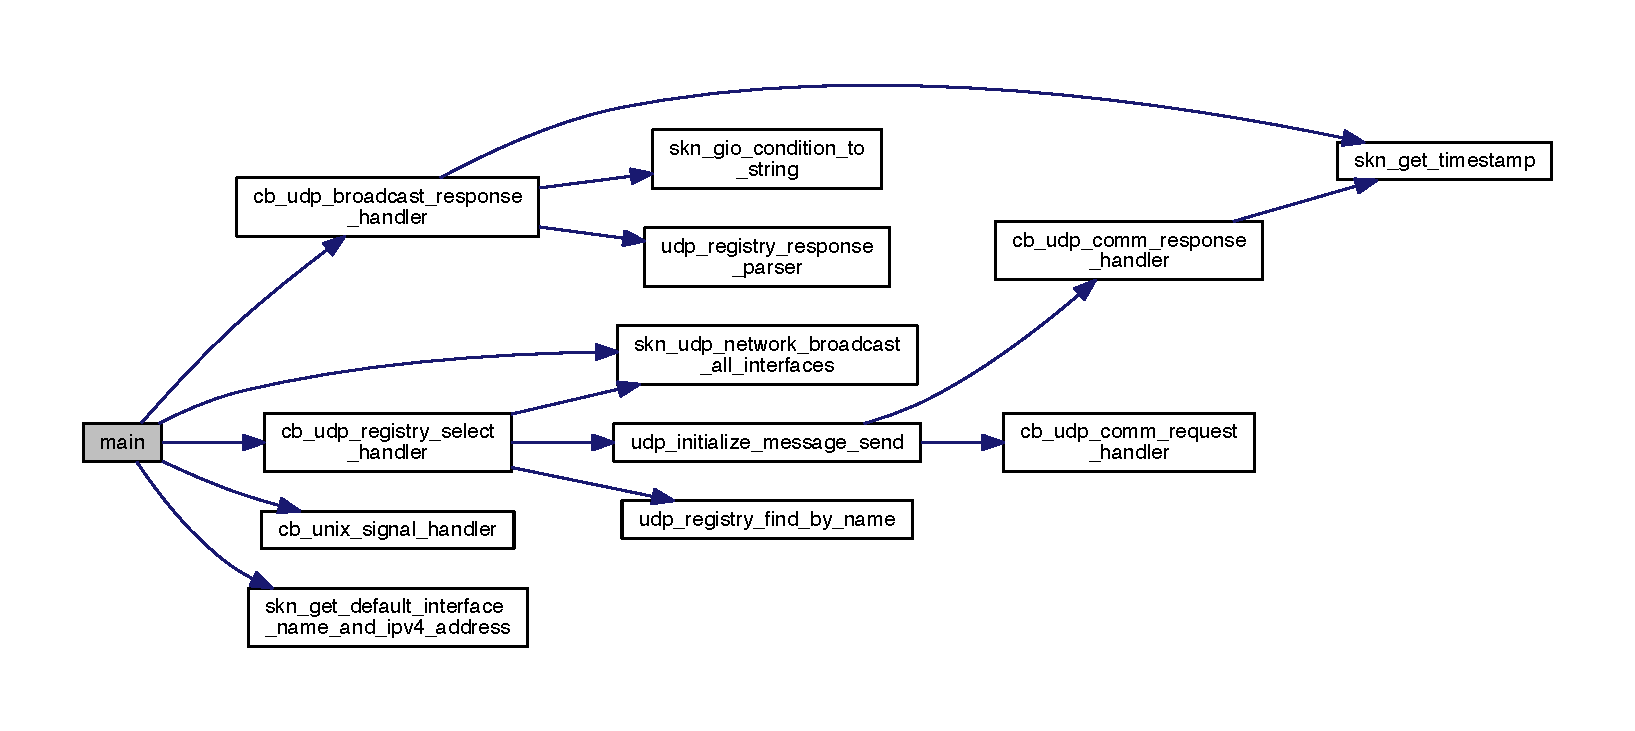
\includegraphics[width=350pt]{cmd_d_c_8c_a3c04138a5bfe5d72780bb7e82a18e627_cgraph}
\end{center}
\end{figure}


\hypertarget{cmd_d_c_8c_a0dfc1a6916909805dc7fd2d8c471e0e3}{}\index{cmd\+D\+C.\+c@{cmd\+D\+C.\+c}!skn\+\_\+get\+\_\+broadcast\+\_\+ip\+\_\+array@{skn\+\_\+get\+\_\+broadcast\+\_\+ip\+\_\+array}}
\index{skn\+\_\+get\+\_\+broadcast\+\_\+ip\+\_\+array@{skn\+\_\+get\+\_\+broadcast\+\_\+ip\+\_\+array}!cmd\+D\+C.\+c@{cmd\+D\+C.\+c}}
\subsubsection[{skn\+\_\+get\+\_\+broadcast\+\_\+ip\+\_\+array(\+P\+I\+P\+Broadcast\+Array pa\+B)}]{\setlength{\rightskip}{0pt plus 5cm}gint skn\+\_\+get\+\_\+broadcast\+\_\+ip\+\_\+array (
\begin{DoxyParamCaption}
\item[{{\bf P\+I\+P\+Broadcast\+Array}}]{pa\+B}
\end{DoxyParamCaption}
)}\label{cmd_d_c_8c_a0dfc1a6916909805dc7fd2d8c471e0e3}
Collect I\+P and Broadcast Addresses for this machine


\begin{DoxyItemize}
\item Affects the P\+I\+P\+Broadcast\+Array
\item Return -\/1 on error, or count of interfaces
\item contains this ip\+Address in pa\+B-\/$>$ip\+Addr\+Str\mbox{[}pa\+B-\/$>$default\+Index\mbox{]} 
\end{DoxyItemize}

Definition at line 185 of file cmd\+D\+C.\+c.



References A\+R\+Y\+\_\+\+M\+A\+X\+\_\+\+I\+N\+T\+F, \+\_\+ip\+Broadcast\+Array\+::broad\+Addr\+Str, \+\_\+ip\+Broadcast\+Array\+::cb\+Name, \+\_\+ip\+Broadcast\+Array\+::ch\+Default\+Intf\+Name, \+\_\+ip\+Broadcast\+Array\+::count, \+\_\+ip\+Broadcast\+Array\+::default\+Index, \+\_\+ip\+Broadcast\+Array\+::if\+Name\+Str, \+\_\+ip\+Broadcast\+Array\+::ip\+Addr\+Str, \+\_\+ip\+Broadcast\+Array\+::mask\+Addr\+Str, P\+L\+A\+T\+F\+O\+R\+M\+\_\+\+E\+R\+R\+O\+R, skn\+\_\+get\+\_\+default\+\_\+interface\+\_\+name(), and S\+Z\+\_\+\+C\+H\+A\+R\+\_\+\+B\+U\+F\+F.



Referenced by skn\+\_\+get\+\_\+default\+\_\+interface\+\_\+name\+\_\+and\+\_\+ipv4\+\_\+address().


\begin{DoxyCode}
185                                                        \{
186     \textcolor{keyword}{struct }ifaddrs * ifap;
187     \textcolor{keyword}{struct }ifaddrs * p;
188     gint rc = 0;
189 
190     memset(paB, 0, \textcolor{keyword}{sizeof}(\hyperlink{struct__ip_broadcast_array}{IPBroadcastArray}));
191     paB->\hyperlink{struct__ip_broadcast_array_a971377a4c995292b8bd908f185cfc844}{count} = 0;
192     paB->\hyperlink{struct__ip_broadcast_array_a5822ff77ae9f31bd3b4298d463c02f1f}{defaultIndex} = 0;
193     strcpy(paB->\hyperlink{struct__ip_broadcast_array_a0f592bd31dcc3ce00a349f04ff6bd1ba}{cbName}, \textcolor{stringliteral}{"IPBroadcastArray"});
194 
195     rc = \hyperlink{cmd_d_c_8c_afc164e6efc7bdcdbacba97ba6f6c2a19}{skn\_get\_default\_interface\_name}(paB->
      \hyperlink{struct__ip_broadcast_array_a06dab8742df19b5aec8538842617778d}{chDefaultIntfName});
196     \textcolor{keywordflow}{if} (rc == EXIT\_FAILURE) \{ \textcolor{comment}{// Alternate method for Mac: 'route -n -A inet'}
197         g\_warning(\textcolor{stringliteral}{"[REGISTRY] No Default Network Interfaces Found!."});
198         paB->\hyperlink{struct__ip_broadcast_array_a06dab8742df19b5aec8538842617778d}{chDefaultIntfName}[0] = 0;
199     \}
200     rc = getifaddrs(&ifap);
201     \textcolor{keywordflow}{if} (rc != 0) \{
202         g\_warning(\textcolor{stringliteral}{"[REGISTRY] No Network Interfaces Found at All ! %d:%d:%s"}, rc, errno, strerror(errno) );
203         \textcolor{keywordflow}{return} (\hyperlink{cmd_d_c_8c_a12efd06fda89d6826f820e75148d8fd7}{PLATFORM\_ERROR});
204     \}
205     p = ifap;
206 
207     \textcolor{keywordflow}{while} (p && (paB->\hyperlink{struct__ip_broadcast_array_a971377a4c995292b8bd908f185cfc844}{count} < \hyperlink{cmd_d_c_8c_a00b19837422a3b13d82b9a525e92ef51}{ARY\_MAX\_INTF})) \{
208         \textcolor{keywordflow}{if} (p->ifa\_addr != NULL && p->ifa\_addr->sa\_family == AF\_INET && ((p->ifa\_flags & IFF\_BROADCAST) > 0
      )) \{
209 
210             inet\_ntop(p->ifa\_addr->sa\_family, &((\textcolor{keyword}{struct} sockaddr\_in *) p->ifa\_addr)->sin\_addr, paB->
      \hyperlink{struct__ip_broadcast_array_a96891ccc707337890b2a166e3ef3a8e1}{ipAddrStr}[paB->\hyperlink{struct__ip_broadcast_array_a971377a4c995292b8bd908f185cfc844}{count}], (\hyperlink{cmd_d_c_8c_a8d2978ad614b0de81c60483e706d9306}{SZ\_CHAR\_BUFF} - 1));
211             inet\_ntop(p->ifa\_addr->sa\_family, &((\textcolor{keyword}{struct} sockaddr\_in *) p->ifa\_netmask)->sin\_addr, paB->
      \hyperlink{struct__ip_broadcast_array_a9241c1fbfb22a3ecfe4777863a063eb3}{maskAddrStr}[paB->\hyperlink{struct__ip_broadcast_array_a971377a4c995292b8bd908f185cfc844}{count}], (\hyperlink{cmd_d_c_8c_a8d2978ad614b0de81c60483e706d9306}{SZ\_CHAR\_BUFF} - 1));
212             inet\_ntop(p->ifa\_addr->sa\_family, &((\textcolor{keyword}{struct} sockaddr\_in *) p->ifa\_broadaddr)->sin\_addr, paB->
      \hyperlink{struct__ip_broadcast_array_af40943e174ba847fa0218cfa6051e277}{broadAddrStr}[paB->\hyperlink{struct__ip_broadcast_array_a971377a4c995292b8bd908f185cfc844}{count}], (\hyperlink{cmd_d_c_8c_a8d2978ad614b0de81c60483e706d9306}{SZ\_CHAR\_BUFF} - 1));
213 
214             strncpy(paB->\hyperlink{struct__ip_broadcast_array_a193b90f271c061e8bf1593bab6a182c9}{ifNameStr}[paB->\hyperlink{struct__ip_broadcast_array_a971377a4c995292b8bd908f185cfc844}{count}], p->ifa\_name, (
      \hyperlink{cmd_d_c_8c_a8d2978ad614b0de81c60483e706d9306}{SZ\_CHAR\_BUFF} -1));
215 
216             \textcolor{comment}{/* Take match as the default */}
217             \textcolor{keywordflow}{if} (strcmp(paB->\hyperlink{struct__ip_broadcast_array_a06dab8742df19b5aec8538842617778d}{chDefaultIntfName}, p->ifa\_name) == 0) \{
218                 paB->\hyperlink{struct__ip_broadcast_array_a5822ff77ae9f31bd3b4298d463c02f1f}{defaultIndex} = paB->\hyperlink{struct__ip_broadcast_array_a971377a4c995292b8bd908f185cfc844}{count};
219             \}
220 
221             paB->\hyperlink{struct__ip_broadcast_array_a971377a4c995292b8bd908f185cfc844}{count}++;
222         \}
223         p = p->ifa\_next;
224     \} \textcolor{comment}{// end while}
225     freeifaddrs(ifap);
226 
227     \textcolor{keywordflow}{return} (paB->\hyperlink{struct__ip_broadcast_array_a971377a4c995292b8bd908f185cfc844}{count});
228 \}
\end{DoxyCode}


Here is the call graph for this function\+:
\nopagebreak
\begin{figure}[H]
\begin{center}
\leavevmode
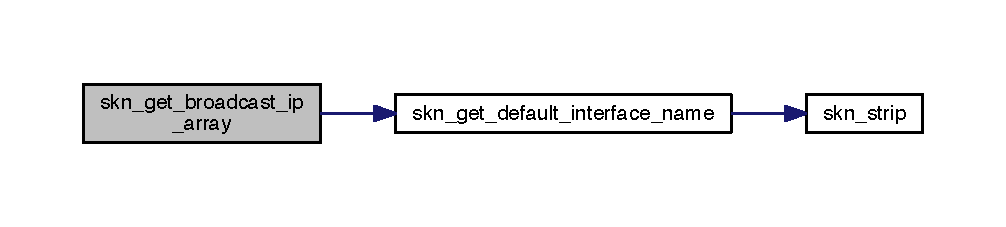
\includegraphics[width=350pt]{cmd_d_c_8c_a0dfc1a6916909805dc7fd2d8c471e0e3_cgraph}
\end{center}
\end{figure}




Here is the caller graph for this function\+:
\nopagebreak
\begin{figure}[H]
\begin{center}
\leavevmode
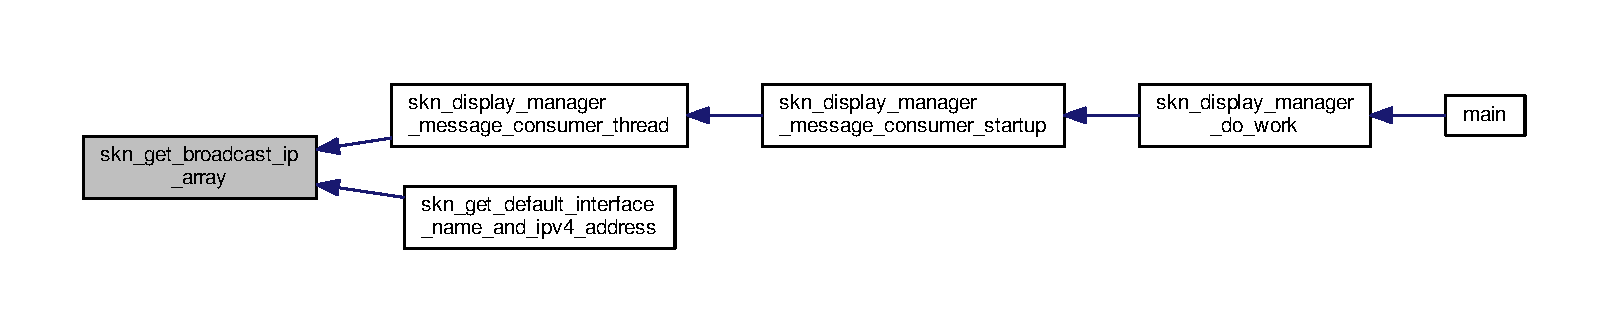
\includegraphics[width=350pt]{cmd_d_c_8c_a0dfc1a6916909805dc7fd2d8c471e0e3_icgraph}
\end{center}
\end{figure}


\hypertarget{cmd_d_c_8c_afc164e6efc7bdcdbacba97ba6f6c2a19}{}\index{cmd\+D\+C.\+c@{cmd\+D\+C.\+c}!skn\+\_\+get\+\_\+default\+\_\+interface\+\_\+name@{skn\+\_\+get\+\_\+default\+\_\+interface\+\_\+name}}
\index{skn\+\_\+get\+\_\+default\+\_\+interface\+\_\+name@{skn\+\_\+get\+\_\+default\+\_\+interface\+\_\+name}!cmd\+D\+C.\+c@{cmd\+D\+C.\+c}}
\subsubsection[{skn\+\_\+get\+\_\+default\+\_\+interface\+\_\+name(char $\ast$pch\+Default\+Interface\+Name)}]{\setlength{\rightskip}{0pt plus 5cm}gint skn\+\_\+get\+\_\+default\+\_\+interface\+\_\+name (
\begin{DoxyParamCaption}
\item[{char $\ast$}]{pch\+Default\+Interface\+Name}
\end{DoxyParamCaption}
)}\label{cmd_d_c_8c_afc164e6efc7bdcdbacba97ba6f6c2a19}
Retrieves default internet interface name into param
\begin{DoxyItemize}
\item absolute best way to do this, but not supported on Darwin(i.\+e O\+S\+X) return E\+X\+I\+T\+\_\+\+S\+U\+C\+C\+E\+S\+S or E\+X\+I\+T\+\_\+\+F\+A\+I\+L\+U\+R\+E
\end{DoxyItemize}

\mbox{[}jscott O\+S\+X\mbox{]}\$ route -\/n get 0.\+0.\+0.\+0 route to\+: default destination\+: default mask\+: default gateway\+: 10.\+21.\+1.\+254 interface\+: en3 flags\+: $<$U\+P,G\+A\+T\+E\+W\+A\+Y,D\+O\+N\+E,S\+T\+A\+T\+I\+C,P\+R\+C\+L\+O\+N\+I\+N\+G$>$ recvpipe sendpipe ssthresh rtt,msec rttvar hopcount mtu expire 0 0 0 0 0 0 1500 0 

Definition at line 246 of file cmd\+D\+C.\+c.



References skn\+\_\+strip(), and S\+Z\+\_\+\+I\+N\+F\+O\+\_\+\+B\+U\+F\+F.



Referenced by skn\+\_\+get\+\_\+broadcast\+\_\+ip\+\_\+array().


\begin{DoxyCode}
246                                                                    \{
247     FILE *f\_route;
248     \textcolor{keywordtype}{char} line[\hyperlink{cmd_d_c_8c_a442d5e93bd9c9d8eb4532aba62b5f86c}{SZ\_INFO\_BUFF}], *dRoute = NULL, *iName = NULL;
249 
250     f\_route = fopen(\textcolor{stringliteral}{"/proc/net/route"}, \textcolor{stringliteral}{"r"});
251     \textcolor{keywordflow}{if} (f\_route != NULL) \{
252         \textcolor{keywordflow}{while} (fgets(line, \hyperlink{cmd_d_c_8c_a442d5e93bd9c9d8eb4532aba62b5f86c}{SZ\_INFO\_BUFF} - 1, f\_route)) \{
253             iName = strtok(line, \textcolor{stringliteral}{"\(\backslash\)t"});
254             dRoute = strtok(NULL, \textcolor{stringliteral}{"\(\backslash\)t"});
255 
256             \textcolor{keywordflow}{if} (iName != NULL && dRoute != NULL) \{
257                 \textcolor{keywordflow}{if} (strcmp(dRoute, \textcolor{stringliteral}{"00000000"}) == 0) \{
258                     strncpy(pchDefaultInterfaceName, iName, (\hyperlink{cmd_d_c_8c_a442d5e93bd9c9d8eb4532aba62b5f86c}{SZ\_INFO\_BUFF} - 1));
259                     \textcolor{keywordflow}{break};
260                 \}
261             \}
262         \}
263         fclose(f\_route);
264 
265         \textcolor{keywordflow}{return} (EXIT\_SUCCESS);
266     \}
267    g\_print(\textcolor{stringliteral}{"[REGISTRY] Opening ProcFs for RouteInfo Failed: %d:%s, Alternate method will be attempted.\(\backslash\)n"}, 
      errno, strerror(errno));
268 
269     f\_route = popen(\textcolor{stringliteral}{"route -n get 0.0.0.0"}, \textcolor{stringliteral}{"r"}); \textcolor{comment}{// for linux 'route -n -A inet', with interface at
       line\_word[7]}
270     \textcolor{keywordflow}{if} (f\_route != NULL) \{
271         \textcolor{keywordflow}{while} (fgets(line, \hyperlink{cmd_d_c_8c_a442d5e93bd9c9d8eb4532aba62b5f86c}{SZ\_INFO\_BUFF} - 1, f\_route)) \{
272             dRoute = strtok(line, \textcolor{stringliteral}{":"});
273             iName = strtok(NULL, \textcolor{stringliteral}{"\(\backslash\)n"});
274             \textcolor{keywordflow}{if} (strcmp(\hyperlink{cmd_d_c_8c_a73ed6790a0276f43dfea595f4cedffa4}{skn\_strip}(dRoute), \textcolor{stringliteral}{"interface"}) == 0) \{
275                 strncpy(pchDefaultInterfaceName, \hyperlink{cmd_d_c_8c_a73ed6790a0276f43dfea595f4cedffa4}{skn\_strip}(iName), (
      \hyperlink{cmd_d_c_8c_a442d5e93bd9c9d8eb4532aba62b5f86c}{SZ\_INFO\_BUFF} - 1));
276                 \textcolor{keywordflow}{break};
277             \}
278         \}
279         fclose(f\_route);
280 
281         \textcolor{keywordflow}{return} (EXIT\_SUCCESS);
282     \} \textcolor{keywordflow}{else} \{
283         g\_warning(\textcolor{stringliteral}{"[REGISTRY] Alternate method to get RouteInfo Failed: %d:%s"}, errno, strerror(errno));
284         \textcolor{keywordflow}{return} (EXIT\_FAILURE);
285     \}
286 
287 \}
\end{DoxyCode}


Here is the call graph for this function\+:
\nopagebreak
\begin{figure}[H]
\begin{center}
\leavevmode
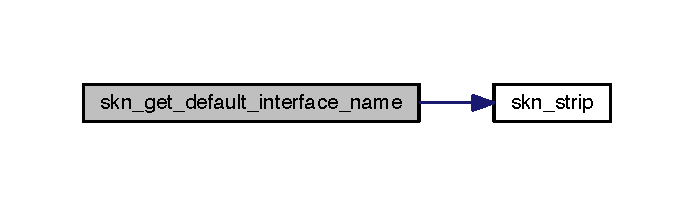
\includegraphics[width=333pt]{cmd_d_c_8c_afc164e6efc7bdcdbacba97ba6f6c2a19_cgraph}
\end{center}
\end{figure}




Here is the caller graph for this function\+:
\nopagebreak
\begin{figure}[H]
\begin{center}
\leavevmode
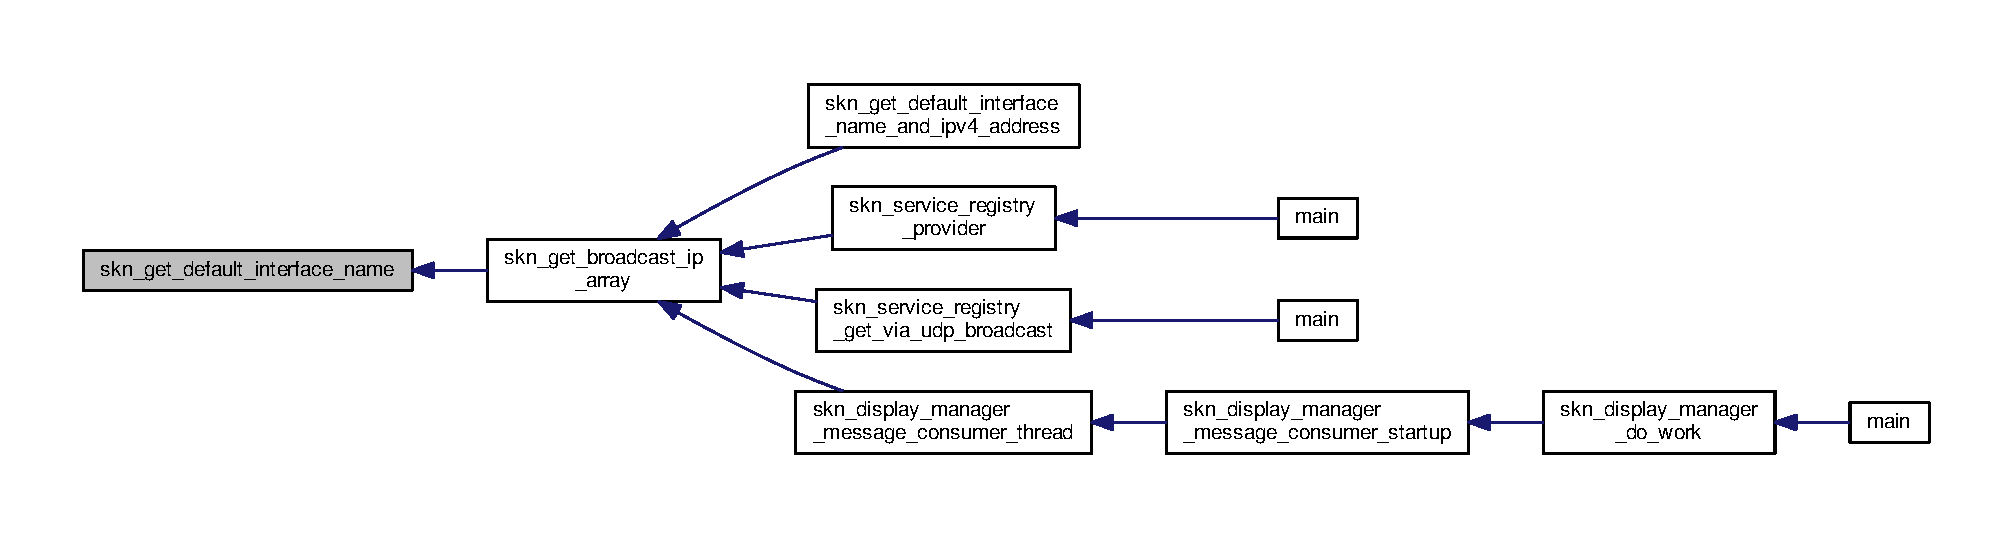
\includegraphics[width=350pt]{cmd_d_c_8c_afc164e6efc7bdcdbacba97ba6f6c2a19_icgraph}
\end{center}
\end{figure}


\hypertarget{cmd_d_c_8c_a72be87baa67e532c78af054acf935d6c}{}\index{cmd\+D\+C.\+c@{cmd\+D\+C.\+c}!skn\+\_\+get\+\_\+default\+\_\+interface\+\_\+name\+\_\+and\+\_\+ipv4\+\_\+address@{skn\+\_\+get\+\_\+default\+\_\+interface\+\_\+name\+\_\+and\+\_\+ipv4\+\_\+address}}
\index{skn\+\_\+get\+\_\+default\+\_\+interface\+\_\+name\+\_\+and\+\_\+ipv4\+\_\+address@{skn\+\_\+get\+\_\+default\+\_\+interface\+\_\+name\+\_\+and\+\_\+ipv4\+\_\+address}!cmd\+D\+C.\+c@{cmd\+D\+C.\+c}}
\subsubsection[{skn\+\_\+get\+\_\+default\+\_\+interface\+\_\+name\+\_\+and\+\_\+ipv4\+\_\+address(char $\ast$intf, char $\ast$ipv4)}]{\setlength{\rightskip}{0pt plus 5cm}{\bf P\+I\+P\+Broadcast\+Array} skn\+\_\+get\+\_\+default\+\_\+interface\+\_\+name\+\_\+and\+\_\+ipv4\+\_\+address (
\begin{DoxyParamCaption}
\item[{char $\ast$}]{intf, }
\item[{char $\ast$}]{ipv4}
\end{DoxyParamCaption}
)}\label{cmd_d_c_8c_a72be87baa67e532c78af054acf935d6c}


Referenced by main().



Here is the caller graph for this function\+:
\nopagebreak
\begin{figure}[H]
\begin{center}
\leavevmode
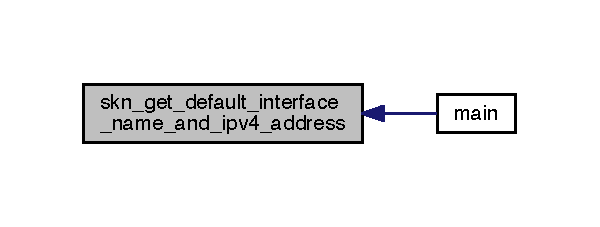
\includegraphics[width=288pt]{cmd_d_c_8c_a72be87baa67e532c78af054acf935d6c_icgraph}
\end{center}
\end{figure}


\hypertarget{cmd_d_c_8c_a4f733621137368e762c5db74a3cec52b}{}\index{cmd\+D\+C.\+c@{cmd\+D\+C.\+c}!skn\+\_\+get\+\_\+default\+\_\+interface\+\_\+name\+\_\+and\+\_\+ipv4\+\_\+address@{skn\+\_\+get\+\_\+default\+\_\+interface\+\_\+name\+\_\+and\+\_\+ipv4\+\_\+address}}
\index{skn\+\_\+get\+\_\+default\+\_\+interface\+\_\+name\+\_\+and\+\_\+ipv4\+\_\+address@{skn\+\_\+get\+\_\+default\+\_\+interface\+\_\+name\+\_\+and\+\_\+ipv4\+\_\+address}!cmd\+D\+C.\+c@{cmd\+D\+C.\+c}}
\subsubsection[{skn\+\_\+get\+\_\+default\+\_\+interface\+\_\+name\+\_\+and\+\_\+ipv4\+\_\+address(gchar $\ast$intf, gchar $\ast$ipv4)}]{\setlength{\rightskip}{0pt plus 5cm}{\bf P\+I\+P\+Broadcast\+Array} skn\+\_\+get\+\_\+default\+\_\+interface\+\_\+name\+\_\+and\+\_\+ipv4\+\_\+address (
\begin{DoxyParamCaption}
\item[{gchar $\ast$}]{intf, }
\item[{gchar $\ast$}]{ipv4}
\end{DoxyParamCaption}
)}\label{cmd_d_c_8c_a4f733621137368e762c5db74a3cec52b}


Definition at line 165 of file cmd\+D\+C.\+c.



References \+\_\+ip\+Broadcast\+Array\+::ch\+Default\+Intf\+Name, \+\_\+ip\+Broadcast\+Array\+::default\+Index, \+\_\+ip\+Broadcast\+Array\+::ip\+Addr\+Str, P\+L\+A\+T\+F\+O\+R\+M\+\_\+\+E\+R\+R\+O\+R, skn\+\_\+get\+\_\+broadcast\+\_\+ip\+\_\+array(), and S\+Z\+\_\+\+C\+H\+A\+R\+\_\+\+B\+U\+F\+F.


\begin{DoxyCode}
165                                                                                               \{
166     \hyperlink{struct__ip_broadcast_array}{PIPBroadcastArray} paB = g\_new0(\hyperlink{struct__ip_broadcast_array}{IPBroadcastArray}, 1);
167 
168     \textcolor{keywordflow}{if} (\hyperlink{cmd_d_c_8c_a0dfc1a6916909805dc7fd2d8c471e0e3}{skn\_get\_broadcast\_ip\_array}(paB) != 
      \hyperlink{cmd_d_c_8c_a12efd06fda89d6826f820e75148d8fd7}{PLATFORM\_ERROR}) \{
169         g\_utf8\_strncpy(intf, paB->\hyperlink{struct__ip_broadcast_array_a06dab8742df19b5aec8538842617778d}{chDefaultIntfName}, 
      \hyperlink{cmd_d_c_8c_a8d2978ad614b0de81c60483e706d9306}{SZ\_CHAR\_BUFF});
170         g\_utf8\_strncpy(ipv4, paB->\hyperlink{struct__ip_broadcast_array_a96891ccc707337890b2a166e3ef3a8e1}{ipAddrStr}[paB->\hyperlink{struct__ip_broadcast_array_a5822ff77ae9f31bd3b4298d463c02f1f}{defaultIndex}], 
      \hyperlink{cmd_d_c_8c_a8d2978ad614b0de81c60483e706d9306}{SZ\_CHAR\_BUFF});
171     \} \textcolor{keywordflow}{else} \{
172         g\_warning(\textcolor{stringliteral}{"[REGISTRY] InterfaceName and Address: unable to access information."});
173         \textcolor{keywordflow}{return}(NULL);
174     \}
175     \textcolor{keywordflow}{return} (paB);
176 \}
\end{DoxyCode}


Here is the call graph for this function\+:
\nopagebreak
\begin{figure}[H]
\begin{center}
\leavevmode
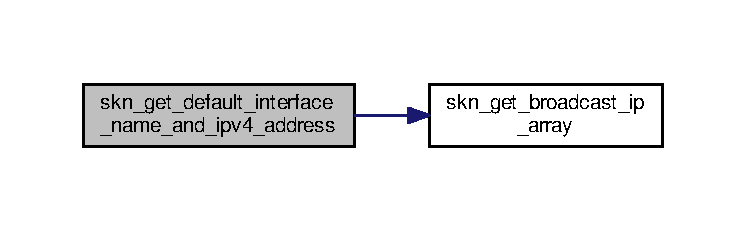
\includegraphics[width=350pt]{cmd_d_c_8c_a4f733621137368e762c5db74a3cec52b_cgraph}
\end{center}
\end{figure}


\hypertarget{cmd_d_c_8c_a8288aea959581188e5bd29430935a6ed}{}\index{cmd\+D\+C.\+c@{cmd\+D\+C.\+c}!skn\+\_\+get\+\_\+timestamp@{skn\+\_\+get\+\_\+timestamp}}
\index{skn\+\_\+get\+\_\+timestamp@{skn\+\_\+get\+\_\+timestamp}!cmd\+D\+C.\+c@{cmd\+D\+C.\+c}}
\subsubsection[{skn\+\_\+get\+\_\+timestamp()}]{\setlength{\rightskip}{0pt plus 5cm}gchar $\ast$ skn\+\_\+get\+\_\+timestamp (
\begin{DoxyParamCaption}
{}
\end{DoxyParamCaption}
)}\label{cmd_d_c_8c_a8288aea959581188e5bd29430935a6ed}


Definition at line 323 of file cmd\+D\+C.\+c.



Referenced by cb\+\_\+udp\+\_\+broadcast\+\_\+response\+\_\+handler(), and cb\+\_\+udp\+\_\+comm\+\_\+response\+\_\+handler().


\begin{DoxyCode}
323                             \{
324     GDateTime   *stamp = g\_date\_time\_new\_now\_local();
325     gchar *response = g\_date\_time\_format(stamp,\textcolor{stringliteral}{"%F.%T"});
326 
327     \textcolor{keywordflow}{return}(response);
328 \}
\end{DoxyCode}


Here is the caller graph for this function\+:
\nopagebreak
\begin{figure}[H]
\begin{center}
\leavevmode
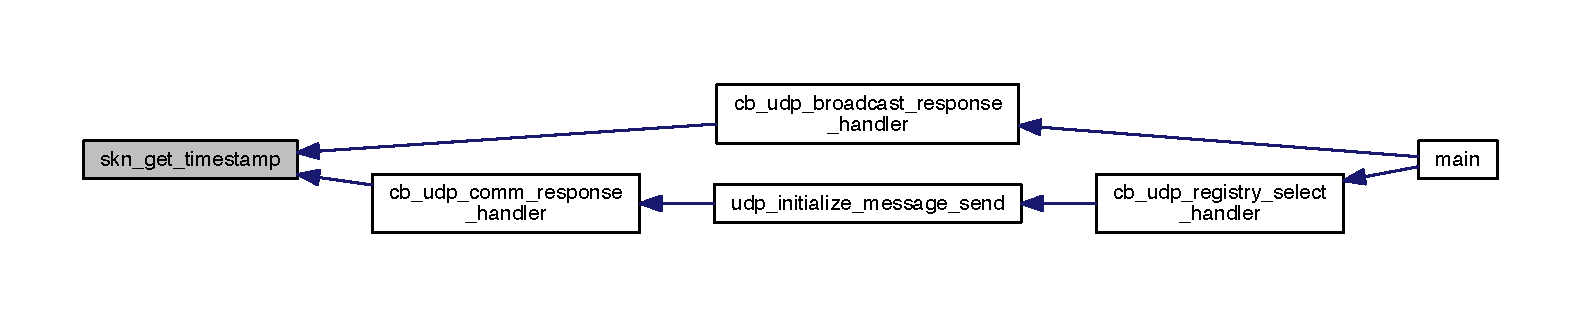
\includegraphics[width=350pt]{cmd_d_c_8c_a8288aea959581188e5bd29430935a6ed_icgraph}
\end{center}
\end{figure}


\hypertarget{cmd_d_c_8c_af4d9de57a3cb296036c837a644009ef5}{}\index{cmd\+D\+C.\+c@{cmd\+D\+C.\+c}!skn\+\_\+gio\+\_\+condition\+\_\+to\+\_\+string@{skn\+\_\+gio\+\_\+condition\+\_\+to\+\_\+string}}
\index{skn\+\_\+gio\+\_\+condition\+\_\+to\+\_\+string@{skn\+\_\+gio\+\_\+condition\+\_\+to\+\_\+string}!cmd\+D\+C.\+c@{cmd\+D\+C.\+c}}
\subsubsection[{skn\+\_\+gio\+\_\+condition\+\_\+to\+\_\+string(\+G\+I\+O\+Condition condition)}]{\setlength{\rightskip}{0pt plus 5cm}gchar $\ast$ skn\+\_\+gio\+\_\+condition\+\_\+to\+\_\+string (
\begin{DoxyParamCaption}
\item[{G\+I\+O\+Condition}]{condition}
\end{DoxyParamCaption}
)}\label{cmd_d_c_8c_af4d9de57a3cb296036c837a644009ef5}


Definition at line 330 of file cmd\+D\+C.\+c.



Referenced by cb\+\_\+udp\+\_\+broadcast\+\_\+response\+\_\+handler().


\begin{DoxyCode}
330                                                             \{
331     gchar *value = NULL;
332 
333     \textcolor{keywordflow}{switch}(condition) \{
334         \textcolor{keywordflow}{case} G\_IO\_IN:
335             value = \textcolor{stringliteral}{"There is data to read."};
336             \textcolor{keywordflow}{break};
337         \textcolor{keywordflow}{case} G\_IO\_OUT:
338             value = \textcolor{stringliteral}{"Data can be written (without blocking)."};
339             \textcolor{keywordflow}{break};
340         \textcolor{keywordflow}{case} G\_IO\_PRI:
341             value = \textcolor{stringliteral}{"There is urgent data to read."};
342             \textcolor{keywordflow}{break};
343         \textcolor{keywordflow}{case} G\_IO\_ERR:
344             value = \textcolor{stringliteral}{"Error condition."};
345             \textcolor{keywordflow}{break};
346         \textcolor{keywordflow}{case} G\_IO\_HUP:
347             value = \textcolor{stringliteral}{"Hung up (the connection has been broken, usually for pipes and sockets)."};
348             \textcolor{keywordflow}{break};
349         \textcolor{keywordflow}{case} G\_IO\_NVAL:
350             value = \textcolor{stringliteral}{"Invalid request. The file descriptor is not open."};
351             \textcolor{keywordflow}{break};
352         \textcolor{keywordflow}{default}:
353             value = \textcolor{stringliteral}{"Unknown GIOCondition!"};
354     \}
355 
356     \textcolor{keywordflow}{return} (value);
357 \}
\end{DoxyCode}


Here is the caller graph for this function\+:
\nopagebreak
\begin{figure}[H]
\begin{center}
\leavevmode
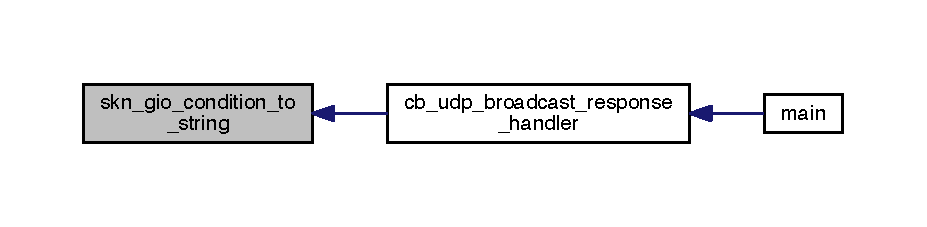
\includegraphics[width=350pt]{cmd_d_c_8c_af4d9de57a3cb296036c837a644009ef5_icgraph}
\end{center}
\end{figure}


\hypertarget{cmd_d_c_8c_a73ed6790a0276f43dfea595f4cedffa4}{}\index{cmd\+D\+C.\+c@{cmd\+D\+C.\+c}!skn\+\_\+strip@{skn\+\_\+strip}}
\index{skn\+\_\+strip@{skn\+\_\+strip}!cmd\+D\+C.\+c@{cmd\+D\+C.\+c}}
\subsubsection[{skn\+\_\+strip(gchar $\ast$alpha)}]{\setlength{\rightskip}{0pt plus 5cm}gchar $\ast$ skn\+\_\+strip (
\begin{DoxyParamCaption}
\item[{gchar $\ast$}]{alpha}
\end{DoxyParamCaption}
)}\label{cmd_d_c_8c_a73ed6790a0276f43dfea595f4cedffa4}
Remove Trailing and Leading Blanks
\begin{DoxyItemize}
\item caution\+: pointers from argv are readonly and segfault on \textquotesingle{}alpha\mbox{[}end\mbox{]} = 0\textquotesingle{} 
\end{DoxyItemize}

Definition at line 139 of file cmd\+D\+C.\+c.



Referenced by skn\+\_\+get\+\_\+default\+\_\+interface\+\_\+name().


\begin{DoxyCode}
139                                  \{
140     \textcolor{keywordflow}{if} (alpha == NULL || strlen(alpha) < 1)
141         \textcolor{keywordflow}{return}(alpha);
142 
143     \textcolor{keywordtype}{int} len = strlen(alpha);
144     \textcolor{keywordtype}{int} end = len - 1;
145     \textcolor{keywordtype}{int} start = 0;
146 
147     \textcolor{comment}{// use isgraph() or !isspace() vs isalnum() to allow ['|' ';' '%']}
148     \textcolor{keywordflow}{while} ( !g\_unichar\_isgraph(alpha[end]) && end > 0 ) \{ \textcolor{comment}{// remove trailing non-alphanumeric chars}
149         alpha[end--] = 0;
150     \}
151 
152     len = strlen(alpha);
153     \textcolor{keywordflow}{while} ( !g\_unichar\_isalnum(alpha[start]) && start < len ) \{ \textcolor{comment}{// find first non-alpha stricter}
154         start++;
155     \}
156     \textcolor{keywordflow}{if} (start < len && start > 0) \{  \textcolor{comment}{// move in place}
157         end = len - start;
158         memmove(&alpha[0], &alpha[start], end);
159         alpha[end] = 0;
160     \}
161 
162     \textcolor{keywordflow}{return}(alpha);
163 \}
\end{DoxyCode}


Here is the caller graph for this function\+:
\nopagebreak
\begin{figure}[H]
\begin{center}
\leavevmode
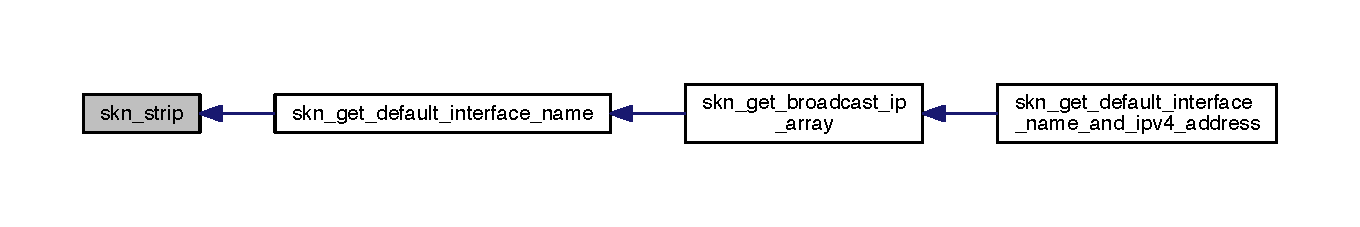
\includegraphics[width=350pt]{cmd_d_c_8c_a73ed6790a0276f43dfea595f4cedffa4_icgraph}
\end{center}
\end{figure}


\hypertarget{cmd_d_c_8c_af376243f65a3fd761050836d1293b0d9}{}\index{cmd\+D\+C.\+c@{cmd\+D\+C.\+c}!skn\+\_\+udp\+\_\+network\+\_\+broadcast\+\_\+all\+\_\+interfaces@{skn\+\_\+udp\+\_\+network\+\_\+broadcast\+\_\+all\+\_\+interfaces}}
\index{skn\+\_\+udp\+\_\+network\+\_\+broadcast\+\_\+all\+\_\+interfaces@{skn\+\_\+udp\+\_\+network\+\_\+broadcast\+\_\+all\+\_\+interfaces}!cmd\+D\+C.\+c@{cmd\+D\+C.\+c}}
\subsubsection[{skn\+\_\+udp\+\_\+network\+\_\+broadcast\+\_\+all\+\_\+interfaces(\+G\+Socket $\ast$g\+Sock, P\+I\+P\+Broadcast\+Array pab)}]{\setlength{\rightskip}{0pt plus 5cm}gboolean skn\+\_\+udp\+\_\+network\+\_\+broadcast\+\_\+all\+\_\+interfaces (
\begin{DoxyParamCaption}
\item[{G\+Socket $\ast$}]{g\+Sock, }
\item[{{\bf P\+I\+P\+Broadcast\+Array}}]{pa\+B}
\end{DoxyParamCaption}
)}\label{cmd_d_c_8c_af376243f65a3fd761050836d1293b0d9}
Send a registry request on the broadcast ip of all interfaces


\begin{DoxyParams}{Parameters}
{\em g\+Sock} & I\+N G\+Lib active/bound socket with broadcast enabled \\
\hline
{\em ch\+\_\+request} & I\+N Greetings message, anytext \\
\hline
{\em ch\+\_\+intf\+Name} & O\+U\+T Default Ethernet Interface Name \\
\hline
{\em ch\+\_\+ip\+Address} & O\+U\+T Default Ethernet I\+P Address \\
\hline
\end{DoxyParams}
\begin{DoxyReturn}{Returns}
true on success, 
\end{DoxyReturn}


Definition at line 297 of file cmd\+D\+C.\+c.



References \+\_\+ip\+Broadcast\+Array\+::broad\+Addr\+Str, \+\_\+ip\+Broadcast\+Array\+::count, \+\_\+ip\+Broadcast\+Array\+::default\+Index, \+\_\+ip\+Broadcast\+Array\+::if\+Name\+Str, \+\_\+ip\+Broadcast\+Array\+::ip\+Addr\+Str, T\+R\+U\+E, and U\+D\+P\+\_\+\+B\+R\+O\+A\+D\+C\+A\+S\+T\+\_\+\+P\+O\+R\+T.



Referenced by cb\+\_\+udp\+\_\+registry\+\_\+select\+\_\+handler(), and main().


\begin{DoxyCode}
297                                                                                          \{
298     \textcolor{keyword}{struct }sockaddr\_in remaddr; \textcolor{comment}{/* remote address */}
299     socklen\_t addrlen = \textcolor{keyword}{sizeof}(remaddr); \textcolor{comment}{/* length of addresses */}
300     gchar *request = \textcolor{stringliteral}{"urn:rpilocator - Rpi Where Are You?"};
301     gint vIndex = 0;
302     gint i\_socket = g\_socket\_get\_fd(gSock);
303 
304     g\_print(\textcolor{stringliteral}{"[REGISTRY] Socket Bound to %s\(\backslash\)n"}, paB->\hyperlink{struct__ip_broadcast_array_a96891ccc707337890b2a166e3ef3a8e1}{ipAddrStr}[paB->
      \hyperlink{struct__ip_broadcast_array_a5822ff77ae9f31bd3b4298d463c02f1f}{defaultIndex}]);
305 
306 
307     \textcolor{keywordflow}{for} (vIndex = 0; vIndex < paB->\hyperlink{struct__ip_broadcast_array_a971377a4c995292b8bd908f185cfc844}{count}; vIndex++) \{
308         memset(&remaddr, 0, \textcolor{keyword}{sizeof}(remaddr));
309         remaddr.sin\_family = AF\_INET;
310         remaddr.sin\_addr.s\_addr = inet\_addr(paB->\hyperlink{struct__ip_broadcast_array_af40943e174ba847fa0218cfa6051e277}{broadAddrStr}[vIndex]);
311         remaddr.sin\_port = htons(\hyperlink{cmd_d_c_8c_a76bd5a574aad0fa67de6c9804853f191}{UDP\_BROADCAST\_PORT});
312 
313         \textcolor{keywordflow}{if} (sendto(i\_socket, request, strlen(request), 0, (\textcolor{keyword}{struct} sockaddr *) &remaddr, addrlen) < 0) \{
314             g\_warning(\textcolor{stringliteral}{"SendTo() Timed out; Failure code=%d, etext=%s"}, errno, strerror(errno));
315             \textcolor{keywordflow}{break};
316         \}
317         g\_print(\textcolor{stringliteral}{"[REGISTRY] Query Broadcasted on %s:%s:%d\(\backslash\)n"}, paB->\hyperlink{struct__ip_broadcast_array_a193b90f271c061e8bf1593bab6a182c9}{ifNameStr}[vIndex], paB->
      \hyperlink{struct__ip_broadcast_array_af40943e174ba847fa0218cfa6051e277}{broadAddrStr}[vIndex], \hyperlink{cmd_d_c_8c_a76bd5a574aad0fa67de6c9804853f191}{UDP\_BROADCAST\_PORT});
318     \}
319 
320     \textcolor{keywordflow}{return}(\hyperlink{skn__common__headers_8h_aa8cecfc5c5c054d2875c03e77b7be15d}{TRUE});
321 \}
\end{DoxyCode}


Here is the caller graph for this function\+:
\nopagebreak
\begin{figure}[H]
\begin{center}
\leavevmode
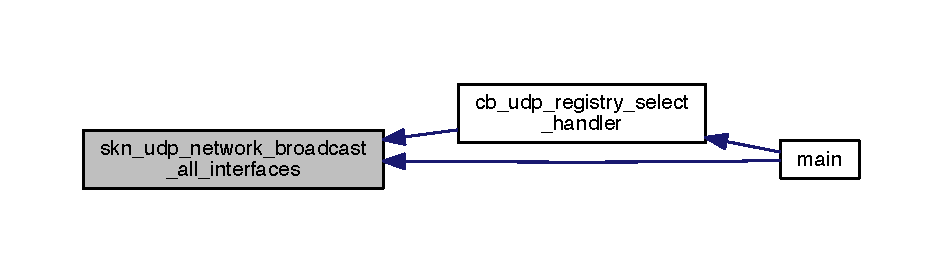
\includegraphics[width=350pt]{cmd_d_c_8c_af376243f65a3fd761050836d1293b0d9_icgraph}
\end{center}
\end{figure}


\hypertarget{cmd_d_c_8c_a793c6b3e5c7a5abc993d8cfbe963629d}{}\index{cmd\+D\+C.\+c@{cmd\+D\+C.\+c}!udp\+\_\+initialize\+\_\+message\+\_\+send@{udp\+\_\+initialize\+\_\+message\+\_\+send}}
\index{udp\+\_\+initialize\+\_\+message\+\_\+send@{udp\+\_\+initialize\+\_\+message\+\_\+send}!cmd\+D\+C.\+c@{cmd\+D\+C.\+c}}
\subsubsection[{udp\+\_\+initialize\+\_\+message\+\_\+send(\+P\+Control\+Data pctrl)}]{\setlength{\rightskip}{0pt plus 5cm}gboolean udp\+\_\+initialize\+\_\+message\+\_\+send (
\begin{DoxyParamCaption}
\item[{{\bf P\+Control\+Data}}]{pctrl}
\end{DoxyParamCaption}
)}\label{cmd_d_c_8c_a793c6b3e5c7a5abc993d8cfbe963629d}


Definition at line 648 of file cmd\+D\+C.\+c.



References cb\+\_\+udp\+\_\+comm\+\_\+request\+\_\+handler(), cb\+\_\+udp\+\_\+comm\+\_\+response\+\_\+handler(), F\+A\+L\+S\+E, \+\_\+control\+Data\+::g\+Comm\+Source, \+\_\+control\+Data\+::g\+Msg\+Delay, \+\_\+control\+Data\+::gs\+Addr, \+\_\+control\+Data\+::g\+Sock, S\+K\+N\+\_\+\+U\+D\+P\+\_\+\+A\+N\+Y\+\_\+\+P\+O\+R\+T, and T\+R\+U\+E.



Referenced by cb\+\_\+udp\+\_\+registry\+\_\+select\+\_\+handler().


\begin{DoxyCode}
648                                                          \{
649     GError *error = NULL;
650     GInetAddress *anyAddr = NULL;
651 
652     g\_return\_val\_if\_fail((NULL != pctrl), G\_SOURCE\_REMOVE);
653 
654     pctrl->\hyperlink{struct__control_data_a49b267275036fc3ac9b7d9e53b0625e1}{gSock} = g\_socket\_new(G\_SOCKET\_FAMILY\_IPV4, G\_SOCKET\_TYPE\_DATAGRAM, G\_SOCKET\_PROTOCOL\_UDP, &
      error);
655     \textcolor{keywordflow}{if} (error != NULL) \{
656         g\_error(\textcolor{stringliteral}{"g\_socket\_new() => %s"}, error->message);
657         g\_clear\_error(&error);
658         \textcolor{keywordflow}{return}(\hyperlink{skn__common__headers_8h_aa93f0eb578d23995850d61f7d61c55c1}{FALSE});
659     \}
660 
661     anyAddr = g\_inet\_address\_new\_any(G\_SOCKET\_FAMILY\_IPV4);
662     pctrl->\hyperlink{struct__control_data_a8a43853386551af4c746fd4b882eb2bf}{gsAddr} = g\_inet\_socket\_address\_new(anyAddr, \hyperlink{cmd_d_c_8c_a8091fbaa709d661a678a82a62fab638b}{SKN\_UDP\_ANY\_PORT});
663         g\_object\_unref(anyAddr);
664 
665     g\_socket\_bind(pctrl->\hyperlink{struct__control_data_a49b267275036fc3ac9b7d9e53b0625e1}{gSock}, pctrl->\hyperlink{struct__control_data_a8a43853386551af4c746fd4b882eb2bf}{gsAddr}, \hyperlink{skn__common__headers_8h_aa8cecfc5c5c054d2875c03e77b7be15d}{TRUE}, &error);
666     \textcolor{keywordflow}{if} (error != NULL) \{
667         g\_error(\textcolor{stringliteral}{"g\_socket\_bind() => %s"}, error->message);
668         g\_clear\_error(&error);
669         exit(\hyperlink{skn__common__headers_8h_aa93f0eb578d23995850d61f7d61c55c1}{FALSE});
670     \}
671 
672     pctrl->\hyperlink{struct__control_data_abfbd9e642ba240fa5985f63d60886de4}{gCommSource} = g\_socket\_create\_source (pctrl->\hyperlink{struct__control_data_a49b267275036fc3ac9b7d9e53b0625e1}{gSock}, G\_IO\_IN, NULL);
673         g\_source\_set\_callback (pctrl->\hyperlink{struct__control_data_abfbd9e642ba240fa5985f63d60886de4}{gCommSource}, (GSourceFunc) 
      \hyperlink{cmd_d_c_8c_aa8a19e68e54683fa324bcee1ecfd3942}{cb\_udp\_comm\_response\_handler}, pctrl, NULL); \textcolor{comment}{// its really a GSocketSourceFunc}
674         g\_source\_attach (pctrl->\hyperlink{struct__control_data_abfbd9e642ba240fa5985f63d60886de4}{gCommSource}, NULL);
675 
676     \textcolor{comment}{/*}
677 \textcolor{comment}{     * Setup Timer to drive repeated Message to Display Service  */}
678     g\_timeout\_add ((pctrl->\hyperlink{struct__control_data_a277ea878a8491fa38269b6c762a05389}{gMsgDelay} * 1000), (GSourceFunc)
      \hyperlink{cmd_d_c_8c_a00c5b52bdcb7caec07d08b05b8c1dced}{cb\_udp\_comm\_request\_handler}, pctrl);
679 
680 
681     \textcolor{keywordflow}{return} (\hyperlink{skn__common__headers_8h_aa8cecfc5c5c054d2875c03e77b7be15d}{TRUE});
682 \}
\end{DoxyCode}


Here is the call graph for this function\+:
\nopagebreak
\begin{figure}[H]
\begin{center}
\leavevmode
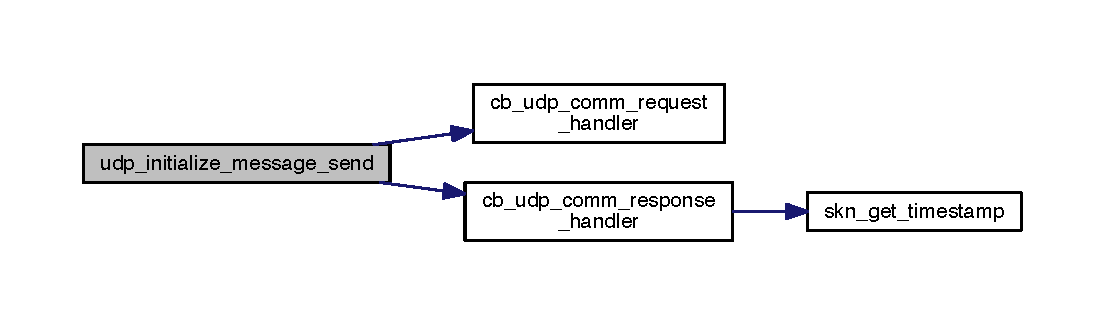
\includegraphics[width=350pt]{cmd_d_c_8c_a793c6b3e5c7a5abc993d8cfbe963629d_cgraph}
\end{center}
\end{figure}




Here is the caller graph for this function\+:
\nopagebreak
\begin{figure}[H]
\begin{center}
\leavevmode
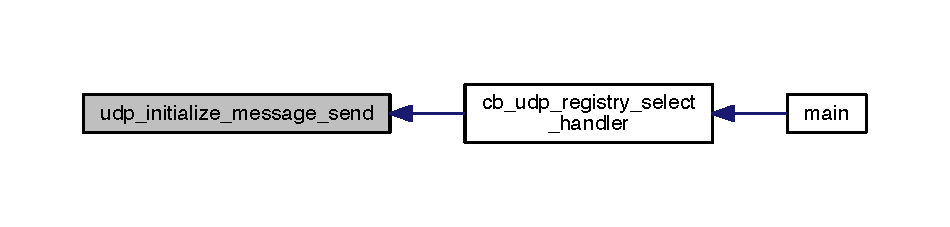
\includegraphics[width=350pt]{cmd_d_c_8c_a793c6b3e5c7a5abc993d8cfbe963629d_icgraph}
\end{center}
\end{figure}


\hypertarget{cmd_d_c_8c_ae59da66ef51690f71da087514886fd12}{}\index{cmd\+D\+C.\+c@{cmd\+D\+C.\+c}!udp\+\_\+registry\+\_\+find\+\_\+by\+\_\+name@{udp\+\_\+registry\+\_\+find\+\_\+by\+\_\+name}}
\index{udp\+\_\+registry\+\_\+find\+\_\+by\+\_\+name@{udp\+\_\+registry\+\_\+find\+\_\+by\+\_\+name}!cmd\+D\+C.\+c@{cmd\+D\+C.\+c}}
\subsubsection[{udp\+\_\+registry\+\_\+find\+\_\+by\+\_\+name(\+P\+Reg\+Data pr, gchar $\ast$pch\+\_\+name)}]{\setlength{\rightskip}{0pt plus 5cm}gint udp\+\_\+registry\+\_\+find\+\_\+by\+\_\+name (
\begin{DoxyParamCaption}
\item[{{\bf P\+Reg\+Data}}]{pr, }
\item[{gchar $\ast$}]{pch\+\_\+name}
\end{DoxyParamCaption}
)}\label{cmd_d_c_8c_ae59da66ef51690f71da087514886fd12}


Definition at line 685 of file cmd\+D\+C.\+c.



References \+\_\+registry\+Data\+::ch\+\_\+name.



Referenced by cb\+\_\+udp\+\_\+registry\+\_\+select\+\_\+handler().


\begin{DoxyCode}
685                                                              \{
686     \textcolor{keywordflow}{return}( g\_strcmp0(pr->\hyperlink{struct__registry_data_a4764e2a72c3ba9177b6c4803cfa03f72}{ch\_name}, pch\_name) );
687 \}
\end{DoxyCode}


Here is the caller graph for this function\+:
\nopagebreak
\begin{figure}[H]
\begin{center}
\leavevmode
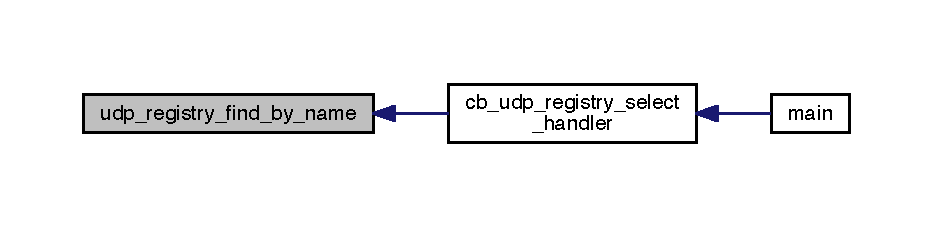
\includegraphics[width=350pt]{cmd_d_c_8c_ae59da66ef51690f71da087514886fd12_icgraph}
\end{center}
\end{figure}


\hypertarget{cmd_d_c_8c_a568a9919cfd345f6c1a41a2ec7c4b1ca}{}\index{cmd\+D\+C.\+c@{cmd\+D\+C.\+c}!udp\+\_\+registry\+\_\+response\+\_\+parser@{udp\+\_\+registry\+\_\+response\+\_\+parser}}
\index{udp\+\_\+registry\+\_\+response\+\_\+parser@{udp\+\_\+registry\+\_\+response\+\_\+parser}!cmd\+D\+C.\+c@{cmd\+D\+C.\+c}}
\subsubsection[{udp\+\_\+registry\+\_\+response\+\_\+parser(\+P\+Reg\+Data msg, gchar $\ast$response)}]{\setlength{\rightskip}{0pt plus 5cm}{\bf P\+P\+Reg\+Data} udp\+\_\+registry\+\_\+response\+\_\+parser (
\begin{DoxyParamCaption}
\item[{{\bf P\+Reg\+Data}}]{msg, }
\item[{gchar $\ast$}]{response}
\end{DoxyParamCaption}
)}\label{cmd_d_c_8c_a568a9919cfd345f6c1a41a2ec7c4b1ca}
Parse this response message

Format\+: name=rpi\+\_\+locator\+\_\+service,ip=10.\+100.\+1.\+19,port=48028$\vert$ name=lcd\+\_\+display\+\_\+service,ip=10.\+100.\+1.\+19,port=48029$\vert$

the vertical bar char \textquotesingle{}$\vert$\textquotesingle{} is the line separator, \% and ; are also supported 

Definition at line 368 of file cmd\+D\+C.\+c.



References \+\_\+registry\+Data\+::ch\+\_\+ip, \+\_\+registry\+Data\+::ch\+\_\+name, \+\_\+registry\+Data\+::ch\+\_\+port, F\+A\+L\+S\+E, S\+Z\+\_\+\+R\+M\+T\+A\+D\+D\+R\+\_\+\+B\+U\+F\+F, and T\+R\+U\+E.



Referenced by cb\+\_\+udp\+\_\+broadcast\+\_\+response\+\_\+handler().


\begin{DoxyCode}
368                                                                       \{
369     gboolean rc = \hyperlink{skn__common__headers_8h_aa93f0eb578d23995850d61f7d61c55c1}{FALSE};
370     gboolean final\_rc = \hyperlink{skn__common__headers_8h_aa93f0eb578d23995850d61f7d61c55c1}{FALSE};
371     gchar ** lines = NULL;
372     gchar *current\_line = NULL;
373     gchar ** entries = NULL;
374     gchar *current\_entry = NULL;
375     gchar ** key\_value = NULL;
376     \hyperlink{struct__registry_data}{PRegData} *msgs;
377     \hyperlink{struct__registry_data}{PRegData} preg = NULL;
378     gint h\_index = 0;
379     gint v\_index = 0;
380     gint o\_index = 0;
381     gint a\_count = 0;
382     gint e\_count = 0;
383 
384     \textcolor{keywordflow}{if} (g\_utf8\_strchr(response, -1, \textcolor{charliteral}{'|'}) == NULL) \{  \textcolor{comment}{// must be a registry entry}
385         \textcolor{keywordflow}{return} (NULL);
386     \}
387 
388     lines = g\_strsplit\_set(response, \textcolor{stringliteral}{"|;%"}, -1);  \textcolor{comment}{// get whole entries}
389     \textcolor{keywordflow}{if} ((NULL == lines) || (g\_strv\_length(lines) < 1)) \{
390         \textcolor{keywordflow}{return}(NULL);
391     \}
392 
393     a\_count = g\_strv\_length(lines);
394     msgs = g\_new0(\hyperlink{struct__registry_data}{PRegData}, a\_count);
395     \textcolor{keywordflow}{for}(o\_index = 0; o\_index < a\_count; o\_index += 1) \{
396         msgs[o\_index] = g\_new0(\hyperlink{struct__registry_data}{RegData}, 1);
397         memmove(msgs[o\_index], msg, \textcolor{keyword}{sizeof}(\hyperlink{struct__registry_data}{RegData}));
398     \}
399 
400     o\_index = 0;
401     current\_line = lines[h\_index];
402     \textcolor{keywordflow}{while} ((NULL != current\_line) && (h\_index < a\_count)) \{   \textcolor{comment}{// do each entry}
403         \textcolor{keywordflow}{if}(g\_utf8\_strlen(current\_line, -1) < 1) \{
404             current\_line = lines[++h\_index];
405             \textcolor{keywordflow}{continue};
406         \}
407 
408         v\_index = 0;
409         entries = g\_strsplit\_set(current\_line, \textcolor{stringliteral}{","}, -1);
410         current\_entry = entries[v\_index];
411         e\_count = g\_strv\_length(entries);
412         preg = msgs[o\_index];
413         rc = \hyperlink{skn__common__headers_8h_aa93f0eb578d23995850d61f7d61c55c1}{FALSE};
414 
415         \textcolor{keywordflow}{while}((NULL != current\_entry) && (v\_index < e\_count)) \{
416             \textcolor{keywordflow}{if}(g\_utf8\_strlen(current\_entry, -1) < 1) \{
417                 current\_entry = entries[++v\_index];
418                 \textcolor{keywordflow}{continue};
419             \}
420 
421             \textcolor{comment}{// get name, ip, port}
422 
423             key\_value = g\_strsplit\_set(current\_entry, \textcolor{stringliteral}{"="}, -1);
424             \textcolor{keywordflow}{if}((key\_value != NULL) && (g\_strv\_length(key\_value) > 0)) \{
425                 \textcolor{keywordflow}{if}(g\_strrstr(key\_value[0], \textcolor{stringliteral}{"a"}) != NULL) \{
426                     final\_rc = rc = \hyperlink{skn__common__headers_8h_aa8cecfc5c5c054d2875c03e77b7be15d}{TRUE};
427                     g\_utf8\_strncpy(preg->\hyperlink{struct__registry_data_a4764e2a72c3ba9177b6c4803cfa03f72}{ch\_name}, key\_value[1], 
      \hyperlink{cmd_d_c_8c_a152ca8fa1a2eac39d1badafb6c6cef8c}{SZ\_RMTADDR\_BUFF});
428                 \}
429                 \textcolor{keywordflow}{if}(g\_strrstr(key\_value[0], \textcolor{stringliteral}{"i"}) != NULL) \{
430                     final\_rc = rc = \hyperlink{skn__common__headers_8h_aa8cecfc5c5c054d2875c03e77b7be15d}{TRUE};
431                     g\_utf8\_strncpy(preg->\hyperlink{struct__registry_data_a814e064e77a6aac5866c88cb51acd971}{ch\_ip}, key\_value[1], 
      \hyperlink{cmd_d_c_8c_a152ca8fa1a2eac39d1badafb6c6cef8c}{SZ\_RMTADDR\_BUFF});
432                 \}
433                 \textcolor{keywordflow}{if}(g\_strrstr(key\_value[0], \textcolor{stringliteral}{"o"}) != NULL) \{
434                     final\_rc = rc = \hyperlink{skn__common__headers_8h_aa8cecfc5c5c054d2875c03e77b7be15d}{TRUE};
435                     g\_utf8\_strncpy(preg->\hyperlink{struct__registry_data_a74f03616af9ec9770266cb7988fe1a71}{ch\_port}, key\_value[1], 
      \hyperlink{cmd_d_c_8c_a152ca8fa1a2eac39d1badafb6c6cef8c}{SZ\_RMTADDR\_BUFF});
436                 \}
437             \}
438             g\_strfreev(key\_value);
439             current\_entry = entries[++v\_index];
440         \} \textcolor{comment}{// end entries}
441 
442         \textcolor{keywordflow}{if} (rc && (g\_utf8\_strlen(preg->\hyperlink{struct__registry_data_a814e064e77a6aac5866c88cb51acd971}{ch\_ip}, -1) > 6)) \{   \textcolor{comment}{// only move if used and valid}
443             o\_index += 1;
444         \}
445         g\_strfreev(entries);
446 
447         h\_index +=1;
448         current\_line = lines[h\_index];
449     \} \textcolor{comment}{// end lines}
450     g\_strfreev(lines);
451 
452     \textcolor{keywordflow}{if} (final\_rc) \{
453         \textcolor{keywordflow}{while}(o\_index < a\_count) \{
454             g\_free(msgs[o\_index]);
455             msgs[o\_index++] = NULL;
456         \}
457         \textcolor{keywordflow}{return}(msgs);
458     \} \textcolor{keywordflow}{else} \{
459         \textcolor{keywordflow}{while}(o\_index < a\_count) \{
460             g\_free(msgs[o\_index]);
461             msgs[o\_index++] = NULL;
462         \}
463         g\_free(msgs);
464         \textcolor{keywordflow}{return}(NULL);
465     \}
466 \}
\end{DoxyCode}


Here is the caller graph for this function\+:
\nopagebreak
\begin{figure}[H]
\begin{center}
\leavevmode
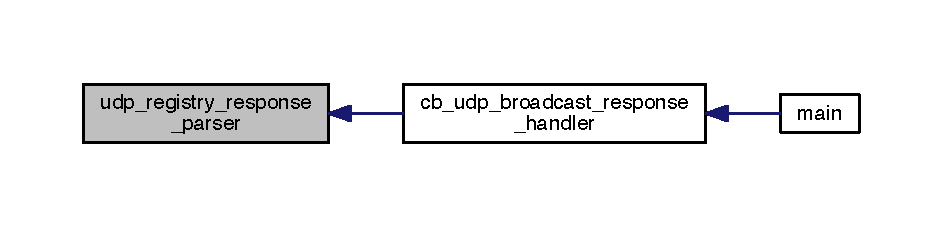
\includegraphics[width=350pt]{cmd_d_c_8c_a568a9919cfd345f6c1a41a2ec7c4b1ca_icgraph}
\end{center}
\end{figure}



\hypertarget{cmd_d_c_2_makefile_8am}{\section{cmd\+D\+C/\+Makefile.am File Reference}
\label{cmd_d_c_2_makefile_8am}\index{cmd\+D\+C/\+Makefile.\+am@{cmd\+D\+C/\+Makefile.\+am}}
}

\hypertarget{cmd_d_s_2_makefile_8am}{}\section{cmd\+D\+S/\+Makefile.am File Reference}
\label{cmd_d_s_2_makefile_8am}\index{cmd\+D\+S/\+Makefile.\+am@{cmd\+D\+S/\+Makefile.\+am}}

\hypertarget{gssdp_d_c_2_makefile_8am}{\section{gssdp\+D\+C/\+Makefile.am File Reference}
\label{gssdp_d_c_2_makefile_8am}\index{gssdp\+D\+C/\+Makefile.\+am@{gssdp\+D\+C/\+Makefile.\+am}}
}

\hypertarget{gtk_d_s_2_makefile_8am}{\section{gtk\+D\+S/\+Makefile.am File Reference}
\label{gtk_d_s_2_makefile_8am}\index{gtk\+D\+S/\+Makefile.\+am@{gtk\+D\+S/\+Makefile.\+am}}
}

\hypertarget{_makefile_8am}{}\section{Makefile.\+am File Reference}
\label{_makefile_8am}\index{Makefile.\+am@{Makefile.\+am}}

\hypertarget{src_2_makefile_8am}{}\section{src/\+Makefile.am File Reference}
\label{src_2_makefile_8am}\index{src/\+Makefile.\+am@{src/\+Makefile.\+am}}

\hypertarget{cmd_d_s_8c}{}\section{cmd\+D\+S/cmd\+D\+S.c File Reference}
\label{cmd_d_s_8c}\index{cmd\+D\+S/cmd\+D\+S.\+c@{cmd\+D\+S/cmd\+D\+S.\+c}}
{\ttfamily \#include $<$stdlib.\+h$>$}\\*
{\ttfamily \#include $<$string.\+h$>$}\\*
{\ttfamily \#include $<$glib.\+h$>$}\\*
{\ttfamily \#include $<$gio/gio.\+h$>$}\\*
{\ttfamily \#include $<$glib-\/unix.\+h$>$}\\*
{\ttfamily \#include $<$gio/gnetworking.\+h$>$}\\*
{\ttfamily \#include $<$ifaddrs.\+h$>$}\\*
Include dependency graph for cmd\+D\+S.\+c\+:
\nopagebreak
\begin{figure}[H]
\begin{center}
\leavevmode
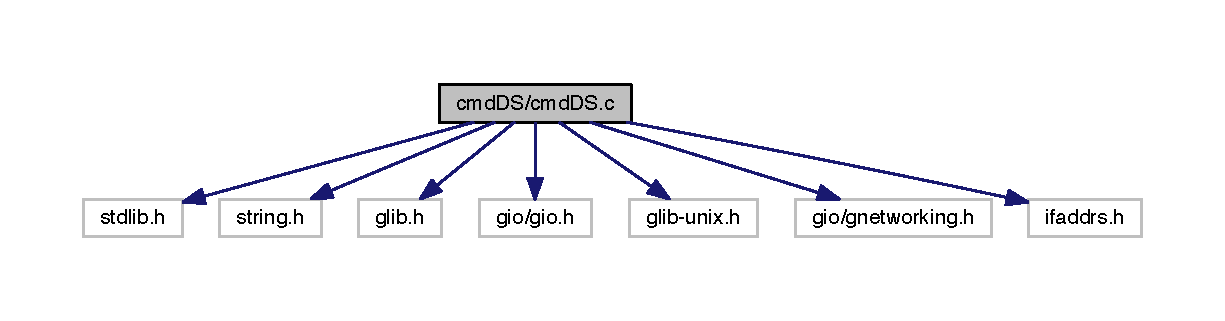
\includegraphics[width=350pt]{cmd_d_s_8c__incl}
\end{center}
\end{figure}
\subsection*{Data Structures}
\begin{DoxyCompactItemize}
\item 
struct \hyperlink{struct__ip_broadcast_array}{\+\_\+ip\+Broadcast\+Array}
\item 
struct \hyperlink{struct__registry_data}{\+\_\+registry\+Data}
\item 
struct \hyperlink{struct__signal_data}{\+\_\+signal\+Data}
\item 
struct \hyperlink{struct__control_data}{\+\_\+control\+Data}
\end{DoxyCompactItemize}
\subsection*{Macros}
\begin{DoxyCompactItemize}
\item 
\#define \hyperlink{cmd_d_s_8c_aa326a05d5e30f9e9a4bb0b4469d5d0c0}{P\+A\+C\+K\+A\+G\+E\+\_\+\+V\+E\+R\+S\+I\+O\+N}~\char`\"{}0.\+9.\+0\char`\"{}
\item 
\#define \hyperlink{cmd_d_s_8c_a1c0439e4355794c09b64274849eb0279}{P\+A\+C\+K\+A\+G\+E\+\_\+\+N\+A\+M\+E}~\char`\"{}cmd\+D\+S\char`\"{}
\item 
\#define \hyperlink{cmd_d_s_8c_a714627d9e7b71b55548e2ddda429d3fb}{P\+A\+C\+K\+A\+G\+E\+\_\+\+D\+E\+S\+C\+R\+I\+P\+T\+I\+O\+N}~\char`\"{}Display Messages from other Raspberry Pi\textquotesingle{}s on the network.\char`\"{}
\item 
\#define \hyperlink{cmd_d_s_8c_a8e8475ded7103e72515667b568ed64c7}{G\+\_\+\+O\+P\+T\+I\+O\+N\+\_\+\+F\+L\+A\+G\+\_\+\+N\+O\+N\+E}~0
\item 
\#define \hyperlink{cmd_d_s_8c_a88c441c906325a3b6b2738e3218e401f}{U\+D\+P\+\_\+\+C\+O\+M\+M\+\_\+\+P\+O\+R\+T}~48029
\item 
\#define \hyperlink{cmd_d_s_8c_a76bd5a574aad0fa67de6c9804853f191}{U\+D\+P\+\_\+\+B\+R\+O\+A\+D\+C\+A\+S\+T\+\_\+\+P\+O\+R\+T}~48028
\item 
\#define \hyperlink{cmd_d_s_8c_af16df2ad6ba0bf1f5283361eb89a979d}{U\+D\+P\+\_\+\+R\+E\+G\+U\+L\+A\+R\+\_\+\+P\+O\+R\+T}~48027
\item 
\#define \hyperlink{cmd_d_s_8c_ac10012e31213e44ecaf5d4c1dd3c8719}{M\+S\+\_\+\+T\+E\+N\+\_\+\+M\+I\+N\+U\+T\+E\+S}~600000
\item 
\#define \hyperlink{cmd_d_s_8c_ac08ad1b127f1c9743c5592ffb796423f}{S\+Z\+\_\+\+T\+I\+M\+E\+S\+T\+A\+M\+P\+\_\+\+B\+U\+F\+F}~32
\item 
\#define \hyperlink{cmd_d_s_8c_ac21e8a77d073e7a5383c92bb485992c8}{S\+Z\+\_\+\+P\+A\+R\+A\+M\+S\+\_\+\+B\+U\+F\+F}~64
\item 
\#define \hyperlink{cmd_d_s_8c_a152ca8fa1a2eac39d1badafb6c6cef8c}{S\+Z\+\_\+\+R\+M\+T\+A\+D\+D\+R\+\_\+\+B\+U\+F\+F}~256
\item 
\#define \hyperlink{cmd_d_s_8c_ab5903aa853c3769389e570c8490feb1e}{S\+Z\+\_\+\+M\+E\+S\+S\+A\+G\+E\+\_\+\+B\+U\+F\+F}~512
\item 
\#define \hyperlink{cmd_d_s_8c_a3c73a8961a16a0dfbb87b5a7317bacd2}{S\+Z\+\_\+\+R\+E\+S\+P\+O\+N\+S\+E\+\_\+\+B\+U\+F\+F}~256
\item 
\#define \hyperlink{cmd_d_s_8c_a3122b900b1a34ceff868e0d51217e357}{S\+Z\+\_\+\+C\+H\+A\+R\+\_\+\+L\+A\+B\+E\+L}~48
\item 
\#define \hyperlink{cmd_d_s_8c_a442d5e93bd9c9d8eb4532aba62b5f86c}{S\+Z\+\_\+\+I\+N\+F\+O\+\_\+\+B\+U\+F\+F}~256
\item 
\#define \hyperlink{cmd_d_s_8c_a8d2978ad614b0de81c60483e706d9306}{S\+Z\+\_\+\+C\+H\+A\+R\+\_\+\+B\+U\+F\+F}~128
\item 
\#define \hyperlink{cmd_d_s_8c_a77ca0b062f899750ee20c0170e5bedc4}{S\+Z\+\_\+\+L\+I\+N\+E\+\_\+\+B\+U\+F\+F}~512
\item 
\#define \hyperlink{cmd_d_s_8c_a352051a682a5205841c1bda6e30bb30d}{S\+Z\+\_\+\+C\+O\+M\+M\+\_\+\+B\+U\+F\+F}~256
\item 
\#define \hyperlink{cmd_d_s_8c_a8091fbaa709d661a678a82a62fab638b}{S\+K\+N\+\_\+\+U\+D\+P\+\_\+\+A\+N\+Y\+\_\+\+P\+O\+R\+T}~0
\item 
\#define \hyperlink{cmd_d_s_8c_a00b19837422a3b13d82b9a525e92ef51}{A\+R\+Y\+\_\+\+M\+A\+X\+\_\+\+I\+N\+T\+F}~8
\item 
\#define \hyperlink{cmd_d_s_8c_a12efd06fda89d6826f820e75148d8fd7}{P\+L\+A\+T\+F\+O\+R\+M\+\_\+\+E\+R\+R\+O\+R}~-\/1
\end{DoxyCompactItemize}
\subsection*{Typedefs}
\begin{DoxyCompactItemize}
\item 
typedef struct \hyperlink{struct__ip_broadcast_array}{\+\_\+ip\+Broadcast\+Array} \hyperlink{cmd_d_s_8c_a83c26957f648dd04df183020ab03c60d}{I\+P\+Broadcast\+Array}
\item 
typedef struct \hyperlink{struct__ip_broadcast_array}{\+\_\+ip\+Broadcast\+Array} $\ast$ \hyperlink{cmd_d_s_8c_a916d712cacebc2faeda930352280c361}{P\+I\+P\+Broadcast\+Array}
\item 
typedef struct \hyperlink{struct__registry_data}{\+\_\+registry\+Data} \hyperlink{cmd_d_s_8c_aac252e0f10021267858720b8e772c0fc}{Reg\+Data}
\item 
typedef struct \hyperlink{struct__registry_data}{\+\_\+registry\+Data} $\ast$ \hyperlink{cmd_d_s_8c_a57f677cfc01b955d9d3783e5422f36a8}{P\+Reg\+Data}
\item 
typedef struct \hyperlink{struct__registry_data}{\+\_\+registry\+Data} $\ast$$\ast$ \hyperlink{cmd_d_s_8c_a0b249e07431f112b20e1708c3162d8a0}{P\+P\+Reg\+Data}
\item 
typedef struct \hyperlink{struct__signal_data}{\+\_\+signal\+Data} \hyperlink{cmd_d_s_8c_a4d86cbb761613143e4ee60218efdfbaa}{U\+Signal\+Data}
\item 
typedef struct \hyperlink{struct__signal_data}{\+\_\+signal\+Data} $\ast$ \hyperlink{cmd_d_s_8c_acdc6976ac4ccc0f13bc99bb5b9361a6e}{P\+U\+Signal\+Data}
\item 
typedef struct \hyperlink{struct__control_data}{\+\_\+control\+Data} \hyperlink{cmd_d_s_8c_aad121cd36cd8851b2a3cd81fd0e41388}{Control\+Data}
\item 
typedef struct \hyperlink{struct__control_data}{\+\_\+control\+Data} $\ast$ \hyperlink{cmd_d_s_8c_aa6bae802f1b23385cd660e89a1e4fc75}{P\+Control\+Data}
\end{DoxyCompactItemize}
\subsection*{Functions}
\begin{DoxyCompactItemize}
\item 
gchar $\ast$ \hyperlink{cmd_d_s_8c_a6ea2e6ee5c8f0d51a98539842634f217}{skn\+\_\+get\+\_\+timestamp} ()
\item 
gchar $\ast$ \hyperlink{cmd_d_s_8c_a5acaf42e0ff80bd0de38c490576e9f85}{skn\+\_\+strip} (gchar $\ast$alpha)
\item 
gchar $\ast$ \hyperlink{cmd_d_s_8c_a2dcc830aabe5f0cfffb3077fc0cba6a5}{skn\+\_\+gio\+\_\+condition\+\_\+to\+\_\+string} (G\+I\+O\+Condition condition)
\item 
\hyperlink{cmd_d_c_8c_a0b249e07431f112b20e1708c3162d8a0}{P\+P\+Reg\+Data} \hyperlink{cmd_d_s_8c_a568a9919cfd345f6c1a41a2ec7c4b1ca}{udp\+\_\+registry\+\_\+response\+\_\+parser} (\hyperlink{cmd_d_c_8c_a57f677cfc01b955d9d3783e5422f36a8}{P\+Reg\+Data} msg, gchar $\ast$response)
\item 
\hyperlink{cmd_d_c_8c_a916d712cacebc2faeda930352280c361}{P\+I\+P\+Broadcast\+Array} \hyperlink{cmd_d_s_8c_a72be87baa67e532c78af054acf935d6c}{skn\+\_\+get\+\_\+default\+\_\+interface\+\_\+name\+\_\+and\+\_\+ipv4\+\_\+address} (char $\ast$intf, char $\ast$ipv4)
\item 
gint \hyperlink{cmd_d_s_8c_a0dfc1a6916909805dc7fd2d8c471e0e3}{skn\+\_\+get\+\_\+broadcast\+\_\+ip\+\_\+array} (\hyperlink{cmd_d_c_8c_a916d712cacebc2faeda930352280c361}{P\+I\+P\+Broadcast\+Array} pa\+B)
\item 
gint \hyperlink{cmd_d_s_8c_afc164e6efc7bdcdbacba97ba6f6c2a19}{skn\+\_\+get\+\_\+default\+\_\+interface\+\_\+name} (char $\ast$pch\+Default\+Interface\+Name)
\item 
gboolean \hyperlink{cmd_d_s_8c_af376243f65a3fd761050836d1293b0d9}{skn\+\_\+udp\+\_\+network\+\_\+broadcast\+\_\+all\+\_\+interfaces} (G\+Socket $\ast$g\+Sock, \hyperlink{cmd_d_c_8c_a916d712cacebc2faeda930352280c361}{P\+I\+P\+Broadcast\+Array} pab)
\item 
static gboolean \hyperlink{cmd_d_s_8c_a76ad4de5945cff6e20dbeff46bda868b}{cb\+\_\+unix\+\_\+signal\+\_\+handler} (\hyperlink{cmd_d_c_8c_acdc6976ac4ccc0f13bc99bb5b9361a6e}{P\+U\+Signal\+Data} psig)
\item 
static gboolean \hyperlink{cmd_d_s_8c_a49f1fa41c6c2b72cbffa3e0399b12ea7}{cb\+\_\+udp\+\_\+request\+\_\+handler} (G\+Socket $\ast$socket, G\+I\+O\+Condition condition, \hyperlink{cmd_d_c_8c_aa6bae802f1b23385cd660e89a1e4fc75}{P\+Control\+Data} pctrl)
\item 
static gboolean \hyperlink{cmd_d_s_8c_a385b710fd30ba190b3b96e814424ff80}{cb\+\_\+udp\+\_\+broadcast\+\_\+response\+\_\+handler} (G\+Socket $\ast$g\+Sock, G\+I\+O\+Condition condition, \hyperlink{cmd_d_c_8c_aa6bae802f1b23385cd660e89a1e4fc75}{P\+Control\+Data} pctrl)
\item 
\hyperlink{cmd_d_c_8c_a916d712cacebc2faeda930352280c361}{P\+I\+P\+Broadcast\+Array} \hyperlink{cmd_d_s_8c_a4f733621137368e762c5db74a3cec52b}{skn\+\_\+get\+\_\+default\+\_\+interface\+\_\+name\+\_\+and\+\_\+ipv4\+\_\+address} (gchar $\ast$intf, gchar $\ast$ipv4)
\item 
int \hyperlink{cmd_d_s_8c_a3c04138a5bfe5d72780bb7e82a18e627}{main} (int argc, char $\ast$$\ast$argv)
\end{DoxyCompactItemize}


\subsection{Macro Definition Documentation}
\hypertarget{cmd_d_s_8c_a00b19837422a3b13d82b9a525e92ef51}{}\index{cmd\+D\+S.\+c@{cmd\+D\+S.\+c}!A\+R\+Y\+\_\+\+M\+A\+X\+\_\+\+I\+N\+T\+F@{A\+R\+Y\+\_\+\+M\+A\+X\+\_\+\+I\+N\+T\+F}}
\index{A\+R\+Y\+\_\+\+M\+A\+X\+\_\+\+I\+N\+T\+F@{A\+R\+Y\+\_\+\+M\+A\+X\+\_\+\+I\+N\+T\+F}!cmd\+D\+S.\+c@{cmd\+D\+S.\+c}}
\subsubsection[{A\+R\+Y\+\_\+\+M\+A\+X\+\_\+\+I\+N\+T\+F}]{\setlength{\rightskip}{0pt plus 5cm}\#define A\+R\+Y\+\_\+\+M\+A\+X\+\_\+\+I\+N\+T\+F~8}\label{cmd_d_s_8c_a00b19837422a3b13d82b9a525e92ef51}


Definition at line 59 of file cmd\+D\+S.\+c.



Referenced by skn\+\_\+get\+\_\+broadcast\+\_\+ip\+\_\+array().

\hypertarget{cmd_d_s_8c_a8e8475ded7103e72515667b568ed64c7}{}\index{cmd\+D\+S.\+c@{cmd\+D\+S.\+c}!G\+\_\+\+O\+P\+T\+I\+O\+N\+\_\+\+F\+L\+A\+G\+\_\+\+N\+O\+N\+E@{G\+\_\+\+O\+P\+T\+I\+O\+N\+\_\+\+F\+L\+A\+G\+\_\+\+N\+O\+N\+E}}
\index{G\+\_\+\+O\+P\+T\+I\+O\+N\+\_\+\+F\+L\+A\+G\+\_\+\+N\+O\+N\+E@{G\+\_\+\+O\+P\+T\+I\+O\+N\+\_\+\+F\+L\+A\+G\+\_\+\+N\+O\+N\+E}!cmd\+D\+S.\+c@{cmd\+D\+S.\+c}}
\subsubsection[{G\+\_\+\+O\+P\+T\+I\+O\+N\+\_\+\+F\+L\+A\+G\+\_\+\+N\+O\+N\+E}]{\setlength{\rightskip}{0pt plus 5cm}\#define G\+\_\+\+O\+P\+T\+I\+O\+N\+\_\+\+F\+L\+A\+G\+\_\+\+N\+O\+N\+E~0}\label{cmd_d_s_8c_a8e8475ded7103e72515667b568ed64c7}


Definition at line 38 of file cmd\+D\+S.\+c.



Referenced by main().

\hypertarget{cmd_d_s_8c_ac10012e31213e44ecaf5d4c1dd3c8719}{}\index{cmd\+D\+S.\+c@{cmd\+D\+S.\+c}!M\+S\+\_\+\+T\+E\+N\+\_\+\+M\+I\+N\+U\+T\+E\+S@{M\+S\+\_\+\+T\+E\+N\+\_\+\+M\+I\+N\+U\+T\+E\+S}}
\index{M\+S\+\_\+\+T\+E\+N\+\_\+\+M\+I\+N\+U\+T\+E\+S@{M\+S\+\_\+\+T\+E\+N\+\_\+\+M\+I\+N\+U\+T\+E\+S}!cmd\+D\+S.\+c@{cmd\+D\+S.\+c}}
\subsubsection[{M\+S\+\_\+\+T\+E\+N\+\_\+\+M\+I\+N\+U\+T\+E\+S}]{\setlength{\rightskip}{0pt plus 5cm}\#define M\+S\+\_\+\+T\+E\+N\+\_\+\+M\+I\+N\+U\+T\+E\+S~600000}\label{cmd_d_s_8c_ac10012e31213e44ecaf5d4c1dd3c8719}


Definition at line 44 of file cmd\+D\+S.\+c.

\hypertarget{cmd_d_s_8c_a714627d9e7b71b55548e2ddda429d3fb}{}\index{cmd\+D\+S.\+c@{cmd\+D\+S.\+c}!P\+A\+C\+K\+A\+G\+E\+\_\+\+D\+E\+S\+C\+R\+I\+P\+T\+I\+O\+N@{P\+A\+C\+K\+A\+G\+E\+\_\+\+D\+E\+S\+C\+R\+I\+P\+T\+I\+O\+N}}
\index{P\+A\+C\+K\+A\+G\+E\+\_\+\+D\+E\+S\+C\+R\+I\+P\+T\+I\+O\+N@{P\+A\+C\+K\+A\+G\+E\+\_\+\+D\+E\+S\+C\+R\+I\+P\+T\+I\+O\+N}!cmd\+D\+S.\+c@{cmd\+D\+S.\+c}}
\subsubsection[{P\+A\+C\+K\+A\+G\+E\+\_\+\+D\+E\+S\+C\+R\+I\+P\+T\+I\+O\+N}]{\setlength{\rightskip}{0pt plus 5cm}\#define P\+A\+C\+K\+A\+G\+E\+\_\+\+D\+E\+S\+C\+R\+I\+P\+T\+I\+O\+N~\char`\"{}Display Messages from other Raspberry Pi\textquotesingle{}s on the network.\char`\"{}}\label{cmd_d_s_8c_a714627d9e7b71b55548e2ddda429d3fb}


Definition at line 26 of file cmd\+D\+S.\+c.

\hypertarget{cmd_d_s_8c_a1c0439e4355794c09b64274849eb0279}{}\index{cmd\+D\+S.\+c@{cmd\+D\+S.\+c}!P\+A\+C\+K\+A\+G\+E\+\_\+\+N\+A\+M\+E@{P\+A\+C\+K\+A\+G\+E\+\_\+\+N\+A\+M\+E}}
\index{P\+A\+C\+K\+A\+G\+E\+\_\+\+N\+A\+M\+E@{P\+A\+C\+K\+A\+G\+E\+\_\+\+N\+A\+M\+E}!cmd\+D\+S.\+c@{cmd\+D\+S.\+c}}
\subsubsection[{P\+A\+C\+K\+A\+G\+E\+\_\+\+N\+A\+M\+E}]{\setlength{\rightskip}{0pt plus 5cm}\#define P\+A\+C\+K\+A\+G\+E\+\_\+\+N\+A\+M\+E~\char`\"{}cmd\+D\+S\char`\"{}}\label{cmd_d_s_8c_a1c0439e4355794c09b64274849eb0279}


Definition at line 23 of file cmd\+D\+S.\+c.

\hypertarget{cmd_d_s_8c_aa326a05d5e30f9e9a4bb0b4469d5d0c0}{}\index{cmd\+D\+S.\+c@{cmd\+D\+S.\+c}!P\+A\+C\+K\+A\+G\+E\+\_\+\+V\+E\+R\+S\+I\+O\+N@{P\+A\+C\+K\+A\+G\+E\+\_\+\+V\+E\+R\+S\+I\+O\+N}}
\index{P\+A\+C\+K\+A\+G\+E\+\_\+\+V\+E\+R\+S\+I\+O\+N@{P\+A\+C\+K\+A\+G\+E\+\_\+\+V\+E\+R\+S\+I\+O\+N}!cmd\+D\+S.\+c@{cmd\+D\+S.\+c}}
\subsubsection[{P\+A\+C\+K\+A\+G\+E\+\_\+\+V\+E\+R\+S\+I\+O\+N}]{\setlength{\rightskip}{0pt plus 5cm}\#define P\+A\+C\+K\+A\+G\+E\+\_\+\+V\+E\+R\+S\+I\+O\+N~\char`\"{}0.\+9.\+0\char`\"{}}\label{cmd_d_s_8c_aa326a05d5e30f9e9a4bb0b4469d5d0c0}
\hyperlink{cmd_d_s_8c}{cmd\+D\+S.\+c} I\+O\+T/\+Raspberry\+Pi message display service gcc -\/v {\ttfamily pkg-\/config -\/-\/cflags -\/-\/libs glib-\/2.\+0 gio-\/2.\+0} -\/\+O3 -\/\+Wall \hyperlink{cmd_d_s_8c}{cmd\+D\+S.\+c} -\/o cmd\+D\+S

Program Flow\+:
\begin{DoxyEnumerate}
\item Initialize -\/$>$ parse\+\_\+options
\item upd\+\_\+broad -\/$>$ loop -\/$>$ receive\+\_\+broadcast\+\_\+message -\/$>$ respond\+\_\+with\+\_\+our\+\_\+registry\+\_\+entry
\end{DoxyEnumerate}
\begin{DoxyEnumerate}
\item upd\+\_\+socket -\/$>$ loop -\/$>$ receive\+\_\+message -\/$>$ log\+\_\+to\+\_\+\+\_\+console
\end{DoxyEnumerate}
\begin{DoxyEnumerate}
\item unix\+\_\+signal -\/$>$ loop -\/$>$ close\+\_\+loop
\item Cleanup -\/$>$ exit 
\end{DoxyEnumerate}

Definition at line 20 of file cmd\+D\+S.\+c.

\hypertarget{cmd_d_s_8c_a12efd06fda89d6826f820e75148d8fd7}{}\index{cmd\+D\+S.\+c@{cmd\+D\+S.\+c}!P\+L\+A\+T\+F\+O\+R\+M\+\_\+\+E\+R\+R\+O\+R@{P\+L\+A\+T\+F\+O\+R\+M\+\_\+\+E\+R\+R\+O\+R}}
\index{P\+L\+A\+T\+F\+O\+R\+M\+\_\+\+E\+R\+R\+O\+R@{P\+L\+A\+T\+F\+O\+R\+M\+\_\+\+E\+R\+R\+O\+R}!cmd\+D\+S.\+c@{cmd\+D\+S.\+c}}
\subsubsection[{P\+L\+A\+T\+F\+O\+R\+M\+\_\+\+E\+R\+R\+O\+R}]{\setlength{\rightskip}{0pt plus 5cm}\#define P\+L\+A\+T\+F\+O\+R\+M\+\_\+\+E\+R\+R\+O\+R~-\/1}\label{cmd_d_s_8c_a12efd06fda89d6826f820e75148d8fd7}


Definition at line 60 of file cmd\+D\+S.\+c.



Referenced by skn\+\_\+get\+\_\+broadcast\+\_\+ip\+\_\+array(), and skn\+\_\+get\+\_\+default\+\_\+interface\+\_\+name\+\_\+and\+\_\+ipv4\+\_\+address().

\hypertarget{cmd_d_s_8c_a8091fbaa709d661a678a82a62fab638b}{}\index{cmd\+D\+S.\+c@{cmd\+D\+S.\+c}!S\+K\+N\+\_\+\+U\+D\+P\+\_\+\+A\+N\+Y\+\_\+\+P\+O\+R\+T@{S\+K\+N\+\_\+\+U\+D\+P\+\_\+\+A\+N\+Y\+\_\+\+P\+O\+R\+T}}
\index{S\+K\+N\+\_\+\+U\+D\+P\+\_\+\+A\+N\+Y\+\_\+\+P\+O\+R\+T@{S\+K\+N\+\_\+\+U\+D\+P\+\_\+\+A\+N\+Y\+\_\+\+P\+O\+R\+T}!cmd\+D\+S.\+c@{cmd\+D\+S.\+c}}
\subsubsection[{S\+K\+N\+\_\+\+U\+D\+P\+\_\+\+A\+N\+Y\+\_\+\+P\+O\+R\+T}]{\setlength{\rightskip}{0pt plus 5cm}\#define S\+K\+N\+\_\+\+U\+D\+P\+\_\+\+A\+N\+Y\+\_\+\+P\+O\+R\+T~0}\label{cmd_d_s_8c_a8091fbaa709d661a678a82a62fab638b}


Definition at line 58 of file cmd\+D\+S.\+c.

\hypertarget{cmd_d_s_8c_a8d2978ad614b0de81c60483e706d9306}{}\index{cmd\+D\+S.\+c@{cmd\+D\+S.\+c}!S\+Z\+\_\+\+C\+H\+A\+R\+\_\+\+B\+U\+F\+F@{S\+Z\+\_\+\+C\+H\+A\+R\+\_\+\+B\+U\+F\+F}}
\index{S\+Z\+\_\+\+C\+H\+A\+R\+\_\+\+B\+U\+F\+F@{S\+Z\+\_\+\+C\+H\+A\+R\+\_\+\+B\+U\+F\+F}!cmd\+D\+S.\+c@{cmd\+D\+S.\+c}}
\subsubsection[{S\+Z\+\_\+\+C\+H\+A\+R\+\_\+\+B\+U\+F\+F}]{\setlength{\rightskip}{0pt plus 5cm}\#define S\+Z\+\_\+\+C\+H\+A\+R\+\_\+\+B\+U\+F\+F~128}\label{cmd_d_s_8c_a8d2978ad614b0de81c60483e706d9306}


Definition at line 54 of file cmd\+D\+S.\+c.



Referenced by skn\+\_\+get\+\_\+broadcast\+\_\+ip\+\_\+array(), and skn\+\_\+get\+\_\+default\+\_\+interface\+\_\+name\+\_\+and\+\_\+ipv4\+\_\+address().

\hypertarget{cmd_d_s_8c_a3122b900b1a34ceff868e0d51217e357}{}\index{cmd\+D\+S.\+c@{cmd\+D\+S.\+c}!S\+Z\+\_\+\+C\+H\+A\+R\+\_\+\+L\+A\+B\+E\+L@{S\+Z\+\_\+\+C\+H\+A\+R\+\_\+\+L\+A\+B\+E\+L}}
\index{S\+Z\+\_\+\+C\+H\+A\+R\+\_\+\+L\+A\+B\+E\+L@{S\+Z\+\_\+\+C\+H\+A\+R\+\_\+\+L\+A\+B\+E\+L}!cmd\+D\+S.\+c@{cmd\+D\+S.\+c}}
\subsubsection[{S\+Z\+\_\+\+C\+H\+A\+R\+\_\+\+L\+A\+B\+E\+L}]{\setlength{\rightskip}{0pt plus 5cm}\#define S\+Z\+\_\+\+C\+H\+A\+R\+\_\+\+L\+A\+B\+E\+L~48}\label{cmd_d_s_8c_a3122b900b1a34ceff868e0d51217e357}


Definition at line 52 of file cmd\+D\+S.\+c.

\hypertarget{cmd_d_s_8c_a352051a682a5205841c1bda6e30bb30d}{}\index{cmd\+D\+S.\+c@{cmd\+D\+S.\+c}!S\+Z\+\_\+\+C\+O\+M\+M\+\_\+\+B\+U\+F\+F@{S\+Z\+\_\+\+C\+O\+M\+M\+\_\+\+B\+U\+F\+F}}
\index{S\+Z\+\_\+\+C\+O\+M\+M\+\_\+\+B\+U\+F\+F@{S\+Z\+\_\+\+C\+O\+M\+M\+\_\+\+B\+U\+F\+F}!cmd\+D\+S.\+c@{cmd\+D\+S.\+c}}
\subsubsection[{S\+Z\+\_\+\+C\+O\+M\+M\+\_\+\+B\+U\+F\+F}]{\setlength{\rightskip}{0pt plus 5cm}\#define S\+Z\+\_\+\+C\+O\+M\+M\+\_\+\+B\+U\+F\+F~256}\label{cmd_d_s_8c_a352051a682a5205841c1bda6e30bb30d}


Definition at line 56 of file cmd\+D\+S.\+c.

\hypertarget{cmd_d_s_8c_a442d5e93bd9c9d8eb4532aba62b5f86c}{}\index{cmd\+D\+S.\+c@{cmd\+D\+S.\+c}!S\+Z\+\_\+\+I\+N\+F\+O\+\_\+\+B\+U\+F\+F@{S\+Z\+\_\+\+I\+N\+F\+O\+\_\+\+B\+U\+F\+F}}
\index{S\+Z\+\_\+\+I\+N\+F\+O\+\_\+\+B\+U\+F\+F@{S\+Z\+\_\+\+I\+N\+F\+O\+\_\+\+B\+U\+F\+F}!cmd\+D\+S.\+c@{cmd\+D\+S.\+c}}
\subsubsection[{S\+Z\+\_\+\+I\+N\+F\+O\+\_\+\+B\+U\+F\+F}]{\setlength{\rightskip}{0pt plus 5cm}\#define S\+Z\+\_\+\+I\+N\+F\+O\+\_\+\+B\+U\+F\+F~256}\label{cmd_d_s_8c_a442d5e93bd9c9d8eb4532aba62b5f86c}


Definition at line 53 of file cmd\+D\+S.\+c.



Referenced by skn\+\_\+get\+\_\+default\+\_\+interface\+\_\+name().

\hypertarget{cmd_d_s_8c_a77ca0b062f899750ee20c0170e5bedc4}{}\index{cmd\+D\+S.\+c@{cmd\+D\+S.\+c}!S\+Z\+\_\+\+L\+I\+N\+E\+\_\+\+B\+U\+F\+F@{S\+Z\+\_\+\+L\+I\+N\+E\+\_\+\+B\+U\+F\+F}}
\index{S\+Z\+\_\+\+L\+I\+N\+E\+\_\+\+B\+U\+F\+F@{S\+Z\+\_\+\+L\+I\+N\+E\+\_\+\+B\+U\+F\+F}!cmd\+D\+S.\+c@{cmd\+D\+S.\+c}}
\subsubsection[{S\+Z\+\_\+\+L\+I\+N\+E\+\_\+\+B\+U\+F\+F}]{\setlength{\rightskip}{0pt plus 5cm}\#define S\+Z\+\_\+\+L\+I\+N\+E\+\_\+\+B\+U\+F\+F~512}\label{cmd_d_s_8c_a77ca0b062f899750ee20c0170e5bedc4}


Definition at line 55 of file cmd\+D\+S.\+c.

\hypertarget{cmd_d_s_8c_ab5903aa853c3769389e570c8490feb1e}{}\index{cmd\+D\+S.\+c@{cmd\+D\+S.\+c}!S\+Z\+\_\+\+M\+E\+S\+S\+A\+G\+E\+\_\+\+B\+U\+F\+F@{S\+Z\+\_\+\+M\+E\+S\+S\+A\+G\+E\+\_\+\+B\+U\+F\+F}}
\index{S\+Z\+\_\+\+M\+E\+S\+S\+A\+G\+E\+\_\+\+B\+U\+F\+F@{S\+Z\+\_\+\+M\+E\+S\+S\+A\+G\+E\+\_\+\+B\+U\+F\+F}!cmd\+D\+S.\+c@{cmd\+D\+S.\+c}}
\subsubsection[{S\+Z\+\_\+\+M\+E\+S\+S\+A\+G\+E\+\_\+\+B\+U\+F\+F}]{\setlength{\rightskip}{0pt plus 5cm}\#define S\+Z\+\_\+\+M\+E\+S\+S\+A\+G\+E\+\_\+\+B\+U\+F\+F~512}\label{cmd_d_s_8c_ab5903aa853c3769389e570c8490feb1e}


Definition at line 49 of file cmd\+D\+S.\+c.

\hypertarget{cmd_d_s_8c_ac21e8a77d073e7a5383c92bb485992c8}{}\index{cmd\+D\+S.\+c@{cmd\+D\+S.\+c}!S\+Z\+\_\+\+P\+A\+R\+A\+M\+S\+\_\+\+B\+U\+F\+F@{S\+Z\+\_\+\+P\+A\+R\+A\+M\+S\+\_\+\+B\+U\+F\+F}}
\index{S\+Z\+\_\+\+P\+A\+R\+A\+M\+S\+\_\+\+B\+U\+F\+F@{S\+Z\+\_\+\+P\+A\+R\+A\+M\+S\+\_\+\+B\+U\+F\+F}!cmd\+D\+S.\+c@{cmd\+D\+S.\+c}}
\subsubsection[{S\+Z\+\_\+\+P\+A\+R\+A\+M\+S\+\_\+\+B\+U\+F\+F}]{\setlength{\rightskip}{0pt plus 5cm}\#define S\+Z\+\_\+\+P\+A\+R\+A\+M\+S\+\_\+\+B\+U\+F\+F~64}\label{cmd_d_s_8c_ac21e8a77d073e7a5383c92bb485992c8}


Definition at line 47 of file cmd\+D\+S.\+c.

\hypertarget{cmd_d_s_8c_a3c73a8961a16a0dfbb87b5a7317bacd2}{}\index{cmd\+D\+S.\+c@{cmd\+D\+S.\+c}!S\+Z\+\_\+\+R\+E\+S\+P\+O\+N\+S\+E\+\_\+\+B\+U\+F\+F@{S\+Z\+\_\+\+R\+E\+S\+P\+O\+N\+S\+E\+\_\+\+B\+U\+F\+F}}
\index{S\+Z\+\_\+\+R\+E\+S\+P\+O\+N\+S\+E\+\_\+\+B\+U\+F\+F@{S\+Z\+\_\+\+R\+E\+S\+P\+O\+N\+S\+E\+\_\+\+B\+U\+F\+F}!cmd\+D\+S.\+c@{cmd\+D\+S.\+c}}
\subsubsection[{S\+Z\+\_\+\+R\+E\+S\+P\+O\+N\+S\+E\+\_\+\+B\+U\+F\+F}]{\setlength{\rightskip}{0pt plus 5cm}\#define S\+Z\+\_\+\+R\+E\+S\+P\+O\+N\+S\+E\+\_\+\+B\+U\+F\+F~256}\label{cmd_d_s_8c_a3c73a8961a16a0dfbb87b5a7317bacd2}


Definition at line 50 of file cmd\+D\+S.\+c.



Referenced by cb\+\_\+udp\+\_\+broadcast\+\_\+response\+\_\+handler().

\hypertarget{cmd_d_s_8c_a152ca8fa1a2eac39d1badafb6c6cef8c}{}\index{cmd\+D\+S.\+c@{cmd\+D\+S.\+c}!S\+Z\+\_\+\+R\+M\+T\+A\+D\+D\+R\+\_\+\+B\+U\+F\+F@{S\+Z\+\_\+\+R\+M\+T\+A\+D\+D\+R\+\_\+\+B\+U\+F\+F}}
\index{S\+Z\+\_\+\+R\+M\+T\+A\+D\+D\+R\+\_\+\+B\+U\+F\+F@{S\+Z\+\_\+\+R\+M\+T\+A\+D\+D\+R\+\_\+\+B\+U\+F\+F}!cmd\+D\+S.\+c@{cmd\+D\+S.\+c}}
\subsubsection[{S\+Z\+\_\+\+R\+M\+T\+A\+D\+D\+R\+\_\+\+B\+U\+F\+F}]{\setlength{\rightskip}{0pt plus 5cm}\#define S\+Z\+\_\+\+R\+M\+T\+A\+D\+D\+R\+\_\+\+B\+U\+F\+F~256}\label{cmd_d_s_8c_a152ca8fa1a2eac39d1badafb6c6cef8c}


Definition at line 48 of file cmd\+D\+S.\+c.



Referenced by udp\+\_\+registry\+\_\+response\+\_\+parser().

\hypertarget{cmd_d_s_8c_ac08ad1b127f1c9743c5592ffb796423f}{}\index{cmd\+D\+S.\+c@{cmd\+D\+S.\+c}!S\+Z\+\_\+\+T\+I\+M\+E\+S\+T\+A\+M\+P\+\_\+\+B\+U\+F\+F@{S\+Z\+\_\+\+T\+I\+M\+E\+S\+T\+A\+M\+P\+\_\+\+B\+U\+F\+F}}
\index{S\+Z\+\_\+\+T\+I\+M\+E\+S\+T\+A\+M\+P\+\_\+\+B\+U\+F\+F@{S\+Z\+\_\+\+T\+I\+M\+E\+S\+T\+A\+M\+P\+\_\+\+B\+U\+F\+F}!cmd\+D\+S.\+c@{cmd\+D\+S.\+c}}
\subsubsection[{S\+Z\+\_\+\+T\+I\+M\+E\+S\+T\+A\+M\+P\+\_\+\+B\+U\+F\+F}]{\setlength{\rightskip}{0pt plus 5cm}\#define S\+Z\+\_\+\+T\+I\+M\+E\+S\+T\+A\+M\+P\+\_\+\+B\+U\+F\+F~32}\label{cmd_d_s_8c_ac08ad1b127f1c9743c5592ffb796423f}


Definition at line 46 of file cmd\+D\+S.\+c.

\hypertarget{cmd_d_s_8c_a76bd5a574aad0fa67de6c9804853f191}{}\index{cmd\+D\+S.\+c@{cmd\+D\+S.\+c}!U\+D\+P\+\_\+\+B\+R\+O\+A\+D\+C\+A\+S\+T\+\_\+\+P\+O\+R\+T@{U\+D\+P\+\_\+\+B\+R\+O\+A\+D\+C\+A\+S\+T\+\_\+\+P\+O\+R\+T}}
\index{U\+D\+P\+\_\+\+B\+R\+O\+A\+D\+C\+A\+S\+T\+\_\+\+P\+O\+R\+T@{U\+D\+P\+\_\+\+B\+R\+O\+A\+D\+C\+A\+S\+T\+\_\+\+P\+O\+R\+T}!cmd\+D\+S.\+c@{cmd\+D\+S.\+c}}
\subsubsection[{U\+D\+P\+\_\+\+B\+R\+O\+A\+D\+C\+A\+S\+T\+\_\+\+P\+O\+R\+T}]{\setlength{\rightskip}{0pt plus 5cm}\#define U\+D\+P\+\_\+\+B\+R\+O\+A\+D\+C\+A\+S\+T\+\_\+\+P\+O\+R\+T~48028}\label{cmd_d_s_8c_a76bd5a574aad0fa67de6c9804853f191}


Definition at line 42 of file cmd\+D\+S.\+c.



Referenced by main(), and skn\+\_\+udp\+\_\+network\+\_\+broadcast\+\_\+all\+\_\+interfaces().

\hypertarget{cmd_d_s_8c_a88c441c906325a3b6b2738e3218e401f}{}\index{cmd\+D\+S.\+c@{cmd\+D\+S.\+c}!U\+D\+P\+\_\+\+C\+O\+M\+M\+\_\+\+P\+O\+R\+T@{U\+D\+P\+\_\+\+C\+O\+M\+M\+\_\+\+P\+O\+R\+T}}
\index{U\+D\+P\+\_\+\+C\+O\+M\+M\+\_\+\+P\+O\+R\+T@{U\+D\+P\+\_\+\+C\+O\+M\+M\+\_\+\+P\+O\+R\+T}!cmd\+D\+S.\+c@{cmd\+D\+S.\+c}}
\subsubsection[{U\+D\+P\+\_\+\+C\+O\+M\+M\+\_\+\+P\+O\+R\+T}]{\setlength{\rightskip}{0pt plus 5cm}\#define U\+D\+P\+\_\+\+C\+O\+M\+M\+\_\+\+P\+O\+R\+T~48029}\label{cmd_d_s_8c_a88c441c906325a3b6b2738e3218e401f}


Definition at line 41 of file cmd\+D\+S.\+c.



Referenced by main().

\hypertarget{cmd_d_s_8c_af16df2ad6ba0bf1f5283361eb89a979d}{}\index{cmd\+D\+S.\+c@{cmd\+D\+S.\+c}!U\+D\+P\+\_\+\+R\+E\+G\+U\+L\+A\+R\+\_\+\+P\+O\+R\+T@{U\+D\+P\+\_\+\+R\+E\+G\+U\+L\+A\+R\+\_\+\+P\+O\+R\+T}}
\index{U\+D\+P\+\_\+\+R\+E\+G\+U\+L\+A\+R\+\_\+\+P\+O\+R\+T@{U\+D\+P\+\_\+\+R\+E\+G\+U\+L\+A\+R\+\_\+\+P\+O\+R\+T}!cmd\+D\+S.\+c@{cmd\+D\+S.\+c}}
\subsubsection[{U\+D\+P\+\_\+\+R\+E\+G\+U\+L\+A\+R\+\_\+\+P\+O\+R\+T}]{\setlength{\rightskip}{0pt plus 5cm}\#define U\+D\+P\+\_\+\+R\+E\+G\+U\+L\+A\+R\+\_\+\+P\+O\+R\+T~48027}\label{cmd_d_s_8c_af16df2ad6ba0bf1f5283361eb89a979d}


Definition at line 43 of file cmd\+D\+S.\+c.



\subsection{Typedef Documentation}
\hypertarget{cmd_d_s_8c_aad121cd36cd8851b2a3cd81fd0e41388}{}\index{cmd\+D\+S.\+c@{cmd\+D\+S.\+c}!Control\+Data@{Control\+Data}}
\index{Control\+Data@{Control\+Data}!cmd\+D\+S.\+c@{cmd\+D\+S.\+c}}
\subsubsection[{Control\+Data}]{\setlength{\rightskip}{0pt plus 5cm}typedef struct {\bf \+\_\+control\+Data}  {\bf Control\+Data}}\label{cmd_d_s_8c_aad121cd36cd8851b2a3cd81fd0e41388}
\hypertarget{cmd_d_s_8c_a83c26957f648dd04df183020ab03c60d}{}\index{cmd\+D\+S.\+c@{cmd\+D\+S.\+c}!I\+P\+Broadcast\+Array@{I\+P\+Broadcast\+Array}}
\index{I\+P\+Broadcast\+Array@{I\+P\+Broadcast\+Array}!cmd\+D\+S.\+c@{cmd\+D\+S.\+c}}
\subsubsection[{I\+P\+Broadcast\+Array}]{\setlength{\rightskip}{0pt plus 5cm}typedef struct {\bf \+\_\+ip\+Broadcast\+Array}  {\bf I\+P\+Broadcast\+Array}}\label{cmd_d_s_8c_a83c26957f648dd04df183020ab03c60d}
\hypertarget{cmd_d_s_8c_aa6bae802f1b23385cd660e89a1e4fc75}{}\index{cmd\+D\+S.\+c@{cmd\+D\+S.\+c}!P\+Control\+Data@{P\+Control\+Data}}
\index{P\+Control\+Data@{P\+Control\+Data}!cmd\+D\+S.\+c@{cmd\+D\+S.\+c}}
\subsubsection[{P\+Control\+Data}]{\setlength{\rightskip}{0pt plus 5cm}typedef struct {\bf \+\_\+control\+Data} $\ast$ {\bf P\+Control\+Data}}\label{cmd_d_s_8c_aa6bae802f1b23385cd660e89a1e4fc75}
\hypertarget{cmd_d_s_8c_a916d712cacebc2faeda930352280c361}{}\index{cmd\+D\+S.\+c@{cmd\+D\+S.\+c}!P\+I\+P\+Broadcast\+Array@{P\+I\+P\+Broadcast\+Array}}
\index{P\+I\+P\+Broadcast\+Array@{P\+I\+P\+Broadcast\+Array}!cmd\+D\+S.\+c@{cmd\+D\+S.\+c}}
\subsubsection[{P\+I\+P\+Broadcast\+Array}]{\setlength{\rightskip}{0pt plus 5cm}typedef struct {\bf \+\_\+ip\+Broadcast\+Array} $\ast$ {\bf P\+I\+P\+Broadcast\+Array}}\label{cmd_d_s_8c_a916d712cacebc2faeda930352280c361}
\hypertarget{cmd_d_s_8c_a0b249e07431f112b20e1708c3162d8a0}{}\index{cmd\+D\+S.\+c@{cmd\+D\+S.\+c}!P\+P\+Reg\+Data@{P\+P\+Reg\+Data}}
\index{P\+P\+Reg\+Data@{P\+P\+Reg\+Data}!cmd\+D\+S.\+c@{cmd\+D\+S.\+c}}
\subsubsection[{P\+P\+Reg\+Data}]{\setlength{\rightskip}{0pt plus 5cm}typedef struct {\bf \+\_\+registry\+Data} $\ast$$\ast$ {\bf P\+P\+Reg\+Data}}\label{cmd_d_s_8c_a0b249e07431f112b20e1708c3162d8a0}
\hypertarget{cmd_d_s_8c_a57f677cfc01b955d9d3783e5422f36a8}{}\index{cmd\+D\+S.\+c@{cmd\+D\+S.\+c}!P\+Reg\+Data@{P\+Reg\+Data}}
\index{P\+Reg\+Data@{P\+Reg\+Data}!cmd\+D\+S.\+c@{cmd\+D\+S.\+c}}
\subsubsection[{P\+Reg\+Data}]{\setlength{\rightskip}{0pt plus 5cm}typedef struct {\bf \+\_\+registry\+Data} $\ast$ {\bf P\+Reg\+Data}}\label{cmd_d_s_8c_a57f677cfc01b955d9d3783e5422f36a8}
\hypertarget{cmd_d_s_8c_acdc6976ac4ccc0f13bc99bb5b9361a6e}{}\index{cmd\+D\+S.\+c@{cmd\+D\+S.\+c}!P\+U\+Signal\+Data@{P\+U\+Signal\+Data}}
\index{P\+U\+Signal\+Data@{P\+U\+Signal\+Data}!cmd\+D\+S.\+c@{cmd\+D\+S.\+c}}
\subsubsection[{P\+U\+Signal\+Data}]{\setlength{\rightskip}{0pt plus 5cm}typedef struct {\bf \+\_\+signal\+Data} $\ast$ {\bf P\+U\+Signal\+Data}}\label{cmd_d_s_8c_acdc6976ac4ccc0f13bc99bb5b9361a6e}
\hypertarget{cmd_d_s_8c_aac252e0f10021267858720b8e772c0fc}{}\index{cmd\+D\+S.\+c@{cmd\+D\+S.\+c}!Reg\+Data@{Reg\+Data}}
\index{Reg\+Data@{Reg\+Data}!cmd\+D\+S.\+c@{cmd\+D\+S.\+c}}
\subsubsection[{Reg\+Data}]{\setlength{\rightskip}{0pt plus 5cm}typedef struct {\bf \+\_\+registry\+Data}  {\bf Reg\+Data}}\label{cmd_d_s_8c_aac252e0f10021267858720b8e772c0fc}
\hypertarget{cmd_d_s_8c_a4d86cbb761613143e4ee60218efdfbaa}{}\index{cmd\+D\+S.\+c@{cmd\+D\+S.\+c}!U\+Signal\+Data@{U\+Signal\+Data}}
\index{U\+Signal\+Data@{U\+Signal\+Data}!cmd\+D\+S.\+c@{cmd\+D\+S.\+c}}
\subsubsection[{U\+Signal\+Data}]{\setlength{\rightskip}{0pt plus 5cm}typedef struct {\bf \+\_\+signal\+Data}  {\bf U\+Signal\+Data}}\label{cmd_d_s_8c_a4d86cbb761613143e4ee60218efdfbaa}


\subsection{Function Documentation}
\hypertarget{cmd_d_s_8c_a385b710fd30ba190b3b96e814424ff80}{}\index{cmd\+D\+S.\+c@{cmd\+D\+S.\+c}!cb\+\_\+udp\+\_\+broadcast\+\_\+response\+\_\+handler@{cb\+\_\+udp\+\_\+broadcast\+\_\+response\+\_\+handler}}
\index{cb\+\_\+udp\+\_\+broadcast\+\_\+response\+\_\+handler@{cb\+\_\+udp\+\_\+broadcast\+\_\+response\+\_\+handler}!cmd\+D\+S.\+c@{cmd\+D\+S.\+c}}
\subsubsection[{cb\+\_\+udp\+\_\+broadcast\+\_\+response\+\_\+handler(\+G\+Socket $\ast$g\+Sock, G\+I\+O\+Condition condition, P\+Control\+Data pctrl)}]{\setlength{\rightskip}{0pt plus 5cm}static gboolean cb\+\_\+udp\+\_\+broadcast\+\_\+response\+\_\+handler (
\begin{DoxyParamCaption}
\item[{G\+Socket $\ast$}]{g\+Sock, }
\item[{G\+I\+O\+Condition}]{condition, }
\item[{{\bf P\+Control\+Data}}]{pctrl}
\end{DoxyParamCaption}
)\hspace{0.3cm}{\ttfamily [static]}}\label{cmd_d_s_8c_a385b710fd30ba190b3b96e814424ff80}


Definition at line 495 of file cmd\+D\+S.\+c.



References \+\_\+registry\+Data\+::ch\+\_\+from, \+\_\+registry\+Data\+::ch\+\_\+ip, \+\_\+registry\+Data\+::ch\+\_\+message, \+\_\+registry\+Data\+::ch\+\_\+name, \+\_\+registry\+Data\+::ch\+\_\+port, \+\_\+control\+Data\+::ch\+\_\+this\+\_\+ip, \+\_\+registry\+Data\+::ch\+\_\+timestamp, \+\_\+control\+Data\+::g\+U\+D\+P\+Port, \+\_\+control\+Data\+::loop, \+\_\+control\+Data\+::pch\+\_\+service\+\_\+name, \+\_\+control\+Data\+::resolver, skn\+\_\+get\+\_\+timestamp(), skn\+\_\+gio\+\_\+condition\+\_\+to\+\_\+string(), S\+Z\+\_\+\+R\+E\+S\+P\+O\+N\+S\+E\+\_\+\+B\+U\+F\+F, and udp\+\_\+registry\+\_\+response\+\_\+parser().



Referenced by main().


\begin{DoxyCode}
495                                                                                                            
         \{
496     GError *error = NULL;
497     GSocketAddress *gsRmtAddr = NULL;
498     GInetAddress *gsAddr = NULL;
499     \hyperlink{struct__registry_data}{PRegData} message = NULL;
500     \hyperlink{struct__registry_data}{PRegData} msg = NULL;
501     \hyperlink{struct__registry_data}{PRegData} *msgs;
502     gchar * rmtHost = NULL;
503     gssize gss\_receive = 0;
504     gchar *stamp = \hyperlink{cmd_d_s_8c_a6ea2e6ee5c8f0d51a98539842634f217}{skn\_get\_timestamp}();
505     gchar response[\hyperlink{cmd_d_s_8c_a3c73a8961a16a0dfbb87b5a7317bacd2}{SZ\_RESPONSE\_BUFF}];
506     gint h\_index = 0;
507     gchar *converted = NULL;
508 
509     \textcolor{keywordflow}{if} ((condition & G\_IO\_HUP) || (condition & G\_IO\_ERR) || (condition & G\_IO\_NVAL)) \{  \textcolor{comment}{/* SHUTDOWN THE
       MAIN LOOP */}
510         g\_message(\textcolor{stringliteral}{"DisplayService::cb\_udp\_broadcast\_response\_handler(error) Operational Error / Shutdown
       Signaled => %s\(\backslash\)n"}, \hyperlink{cmd_d_s_8c_a2dcc830aabe5f0cfffb3077fc0cba6a5}{skn\_gio\_condition\_to\_string}(condition));
511         g\_main\_loop\_quit(pctrl->\hyperlink{struct__control_data_ae1b70bafbd5eb568c6ca339664959216}{loop});
512         \textcolor{keywordflow}{return} ( G\_SOURCE\_REMOVE );
513     \}
514     \textcolor{keywordflow}{if} (condition != G\_IO\_IN) \{
515         g\_message(\textcolor{stringliteral}{"DisplayService::cb\_udp\_broadcast\_response\_handler(error) NOT G\_IO\_IN => %s\(\backslash\)n"}, 
      \hyperlink{cmd_d_s_8c_a2dcc830aabe5f0cfffb3077fc0cba6a5}{skn\_gio\_condition\_to\_string}(condition));
516         \textcolor{keywordflow}{return} (G\_SOURCE\_CONTINUE);
517     \}
518 
519     \textcolor{comment}{/*}
520 \textcolor{comment}{     * Allocate a new queue message and read incoming request directly into it */}
521     message = g\_new0(\hyperlink{struct__registry_data}{RegData},1);
522 
523     \textcolor{comment}{/*}
524 \textcolor{comment}{     * If socket times out before reading data any operation will error with 'G\_IO\_ERROR\_TIMED\_OUT'.}
525 \textcolor{comment}{     * Read Request Message and get Requestor IP Address or Name}
526 \textcolor{comment}{    */}
527     gss\_receive = g\_socket\_receive\_from (gSock, &gsRmtAddr, message->\hyperlink{struct__registry_data_ae9b0c1e6f13d980dcc7515def6b20b5e}{ch\_message}, \textcolor{keyword}{sizeof}(message->
      \hyperlink{struct__registry_data_ae9b0c1e6f13d980dcc7515def6b20b5e}{ch\_message}), NULL, &error);
528     \textcolor{keywordflow}{if} (error != NULL) \{ \textcolor{comment}{// gss\_receive = Number of bytes read, or 0 if the connection was closed by the
       peer, or -1 on error}
529         g\_error(\textcolor{stringliteral}{"g\_socket\_receive\_from() => %s"}, error->message);
530         g\_clear\_error(&error);
531         g\_free(message);
532         g\_free(stamp);
533         \textcolor{keywordflow}{return} (G\_SOURCE\_CONTINUE);
534     \}
535     \textcolor{keywordflow}{if} (gss\_receive > 0 ) \{
536         \textcolor{keywordflow}{if} (G\_IS\_INET\_SOCKET\_ADDRESS(gsRmtAddr) ) \{
537             gsAddr = g\_inet\_socket\_address\_get\_address( G\_INET\_SOCKET\_ADDRESS(gsRmtAddr) );
538             \textcolor{keywordflow}{if} ( G\_IS\_INET\_ADDRESS(gsAddr) ) \{
539                 g\_object\_ref(gsAddr);
540                 rmtHost = g\_resolver\_lookup\_by\_address (pctrl->\hyperlink{struct__control_data_afe33a7083e1ecc9ba50a69644ed4a753}{resolver}, gsAddr, NULL, NULL);
541                 \textcolor{keywordflow}{if} (NULL == rmtHost) \{
542                     rmtHost = g\_inet\_address\_to\_string ( gsAddr);
543                 \}
544             \}
545         \}
546 
547         \textcolor{comment}{/*}
548 \textcolor{comment}{         * Convert to UTF8}
549 \textcolor{comment}{         */}
550         converted = g\_convert (message->\hyperlink{struct__registry_data_ae9b0c1e6f13d980dcc7515def6b20b5e}{ch\_message}, gss\_receive, \textcolor{stringliteral}{"UTF-8"}, \textcolor{stringliteral}{"ISO-8859-1"}, NULL, 
      NULL, NULL);
551         \textcolor{keywordflow}{if} (NULL != converted) \{
552             g\_utf8\_strncpy(message->\hyperlink{struct__registry_data_ae9b0c1e6f13d980dcc7515def6b20b5e}{ch\_message}, converted, \textcolor{keyword}{sizeof}(message->
      \hyperlink{struct__registry_data_ae9b0c1e6f13d980dcc7515def6b20b5e}{ch\_message}));
553             g\_free(converted);
554         \}
555 
556         g\_utf8\_strncpy(message->\hyperlink{struct__registry_data_a362a4edf89daafe79565053dd70892c4}{ch\_timestamp}, stamp, \textcolor{keyword}{sizeof}(message->
      \hyperlink{struct__registry_data_a362a4edf89daafe79565053dd70892c4}{ch\_timestamp}));
557         g\_utf8\_strncpy(message->\hyperlink{struct__registry_data_a5fac46820690525a9d8b3f0185bca587}{ch\_from},      rmtHost, \textcolor{keyword}{sizeof}(message->
      \hyperlink{struct__registry_data_a5fac46820690525a9d8b3f0185bca587}{ch\_from}));
558         \textcolor{keywordflow}{if} ( (msgs = \hyperlink{cmd_d_s_8c_a568a9919cfd345f6c1a41a2ec7c4b1ca}{udp\_registry\_response\_parser}(message, message->
      \hyperlink{struct__registry_data_ae9b0c1e6f13d980dcc7515def6b20b5e}{ch\_message})) != NULL ) \{
559             \textcolor{comment}{/*}
560 \textcolor{comment}{             * Send it to be processed by a message handler */}
561             g\_free(message);
562             h\_index = 0;
563             msg = (\hyperlink{cmd_d_s_8c_a57f677cfc01b955d9d3783e5422f36a8}{PRegData})msgs[h\_index];
564             \textcolor{keywordflow}{while} ( msg != NULL ) \{
565                 g\_print(\textcolor{stringliteral}{"[REGISTRY] From=%s, Node=%s, IP=%s, Port=%s\(\backslash\)n"}, msg->
      \hyperlink{struct__registry_data_a5fac46820690525a9d8b3f0185bca587}{ch\_from}, msg->\hyperlink{struct__registry_data_a4764e2a72c3ba9177b6c4803cfa03f72}{ch\_name}, msg->\hyperlink{struct__registry_data_a814e064e77a6aac5866c88cb51acd971}{ch\_ip}, msg->\hyperlink{struct__registry_data_a74f03616af9ec9770266cb7988fe1a71}{ch\_port});
566                 g\_free(msg);
567                 msg = (\hyperlink{cmd_d_s_8c_a57f677cfc01b955d9d3783e5422f36a8}{PRegData})msgs[++h\_index];
568             \}
569             g\_free(msgs);
570         \} \textcolor{keywordflow}{else} \{
571             g\_free(message);
572 
573             \textcolor{comment}{/* Format: name=rpi\_locator\_service,ip=10.100.1.19,port=48028|}
574 \textcolor{comment}{             *         name=cmdline\_display\_service,ip=10.100.1.19,port=48029|}
575 \textcolor{comment}{             */}
576 
577             g\_snprintf(response, \textcolor{keyword}{sizeof}(response),
578                        \textcolor{stringliteral}{"name=rpi\_locator\_service,ip=%s,port=48028|name=%s,ip=%s,port=%d|"},
579                        pctrl->\hyperlink{struct__control_data_ac48fc4263dd4a6bad484b93fbf1ffe1b}{ch\_this\_ip}, pctrl->\hyperlink{struct__control_data_a2197fd3d9315510193866dbedbd3cc8b}{pch\_service\_name}, pctrl->
      \hyperlink{struct__control_data_ac48fc4263dd4a6bad484b93fbf1ffe1b}{ch\_this\_ip}, pctrl->\hyperlink{struct__control_data_a78b36762a9d85d027fc5e41576ade4f7}{gUDPPort});
580             \textcolor{comment}{/*}
581 \textcolor{comment}{             * Send Registry Response to caller */}
582             g\_socket\_send\_to (gSock, gsRmtAddr, response, strlen(response), NULL, &error);
583             \textcolor{keywordflow}{if} (error != NULL) \{  \textcolor{comment}{// gss\_send = Number of bytes written (which may be less than size ), or
       -1 on error}
584                 g\_error(\textcolor{stringliteral}{"g\_socket\_send\_to() => %s"}, error->message);
585                 g\_free(message);
586                 g\_clear\_error(&error);
587             \}
588         \}
589     \}
590     g\_free(stamp);
591     g\_free(rmtHost);
592 
593     \textcolor{keywordflow}{if} ( G\_IS\_INET\_ADDRESS(gsAddr) )
594         g\_object\_unref(gsAddr);
595 
596     \textcolor{keywordflow}{if} ( G\_IS\_INET\_SOCKET\_ADDRESS(gsRmtAddr) )
597         g\_object\_unref(gsRmtAddr);
598 
599     \textcolor{keywordflow}{return} (G\_SOURCE\_CONTINUE);
600 \}
\end{DoxyCode}


Here is the call graph for this function\+:
\nopagebreak
\begin{figure}[H]
\begin{center}
\leavevmode
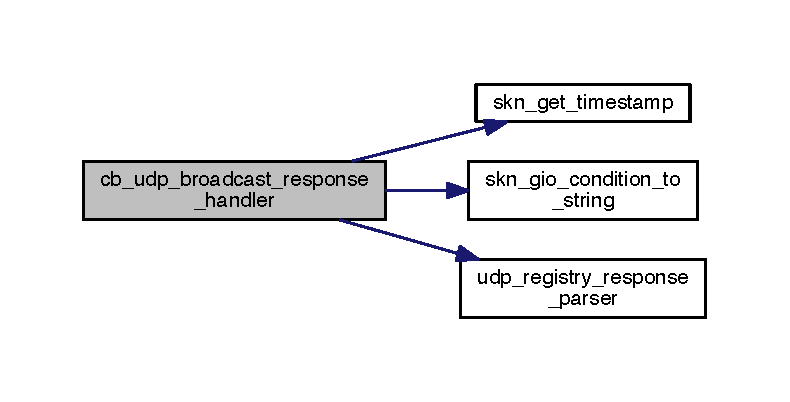
\includegraphics[width=350pt]{cmd_d_s_8c_a385b710fd30ba190b3b96e814424ff80_cgraph}
\end{center}
\end{figure}




Here is the caller graph for this function\+:
\nopagebreak
\begin{figure}[H]
\begin{center}
\leavevmode
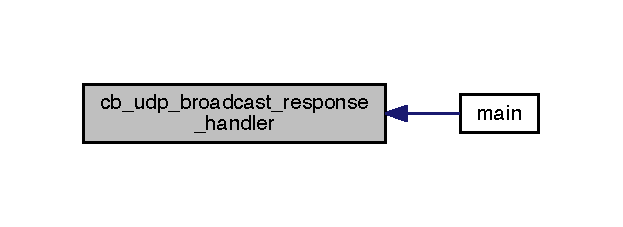
\includegraphics[width=299pt]{cmd_d_s_8c_a385b710fd30ba190b3b96e814424ff80_icgraph}
\end{center}
\end{figure}


\hypertarget{cmd_d_s_8c_a49f1fa41c6c2b72cbffa3e0399b12ea7}{}\index{cmd\+D\+S.\+c@{cmd\+D\+S.\+c}!cb\+\_\+udp\+\_\+request\+\_\+handler@{cb\+\_\+udp\+\_\+request\+\_\+handler}}
\index{cb\+\_\+udp\+\_\+request\+\_\+handler@{cb\+\_\+udp\+\_\+request\+\_\+handler}!cmd\+D\+S.\+c@{cmd\+D\+S.\+c}}
\subsubsection[{cb\+\_\+udp\+\_\+request\+\_\+handler(\+G\+Socket $\ast$socket, G\+I\+O\+Condition condition, P\+Control\+Data pctrl)}]{\setlength{\rightskip}{0pt plus 5cm}static gboolean cb\+\_\+udp\+\_\+request\+\_\+handler (
\begin{DoxyParamCaption}
\item[{G\+Socket $\ast$}]{socket, }
\item[{G\+I\+O\+Condition}]{condition, }
\item[{{\bf P\+Control\+Data}}]{pctrl}
\end{DoxyParamCaption}
)\hspace{0.3cm}{\ttfamily [static]}}\label{cmd_d_s_8c_a49f1fa41c6c2b72cbffa3e0399b12ea7}


Definition at line 429 of file cmd\+D\+S.\+c.



References \+\_\+control\+Data\+::ch\+\_\+read, \+\_\+control\+Data\+::ch\+\_\+request, \+\_\+control\+Data\+::ch\+\_\+response, \+\_\+control\+Data\+::loop, \+\_\+control\+Data\+::resolver, skn\+\_\+get\+\_\+timestamp(), and skn\+\_\+gio\+\_\+condition\+\_\+to\+\_\+string().



Referenced by main().


\begin{DoxyCode}
429                                                                                                    \{
430     GError *error = NULL;
431     GSocketAddress *gsRmtAddr = NULL;
432     GInetAddress *gsAddr = NULL;
433     gchar * rmtHost = NULL;
434     gchar *stamp = \hyperlink{cmd_d_s_8c_a6ea2e6ee5c8f0d51a98539842634f217}{skn\_get\_timestamp}();
435     gssize gss\_receive = 0;
436 
437     \textcolor{keywordflow}{if} ((condition & G\_IO\_HUP) || (condition & G\_IO\_ERR) || (condition & G\_IO\_NVAL)) \{  \textcolor{comment}{/* SHUTDOWN THE
       MAIN LOOP */}
438         g\_message(\textcolor{stringliteral}{"DisplayService::cb\_udp\_request\_handler(error) G\_IO\_HUP => %s\(\backslash\)n"}, 
      \hyperlink{cmd_d_s_8c_a2dcc830aabe5f0cfffb3077fc0cba6a5}{skn\_gio\_condition\_to\_string}(condition));
439         g\_main\_loop\_quit(pctrl->\hyperlink{struct__control_data_ae1b70bafbd5eb568c6ca339664959216}{loop});
440         \textcolor{keywordflow}{return} ( G\_SOURCE\_REMOVE );
441     \}
442     \textcolor{keywordflow}{if} (condition != G\_IO\_IN) \{
443         g\_message(\textcolor{stringliteral}{"DisplayService::cb\_udp\_request\_handler(error) NOT G\_IO\_IN => %s\(\backslash\)n"}, 
      \hyperlink{cmd_d_s_8c_a2dcc830aabe5f0cfffb3077fc0cba6a5}{skn\_gio\_condition\_to\_string}(condition));
444         \textcolor{keywordflow}{return} (G\_SOURCE\_CONTINUE);
445     \}
446 
447     \textcolor{comment}{/*}
448 \textcolor{comment}{     * If socket times out before reading data any operation will error with 'G\_IO\_ERROR\_TIMED\_OUT'.}
449 \textcolor{comment}{    */}
450     gss\_receive = g\_socket\_receive\_from (gSock, &gsRmtAddr, pctrl->\hyperlink{struct__control_data_a243b075becb92f2f37f56f60f738efb1}{ch\_read}, \textcolor{keyword}{sizeof}(pctrl->
      \hyperlink{struct__control_data_a243b075becb92f2f37f56f60f738efb1}{ch\_read}), NULL, &error);
451     \textcolor{keywordflow}{if} (error != NULL) \{ \textcolor{comment}{// gss\_receive = Number of bytes read, or 0 if the connection was closed by the
       peer, or -1 on error}
452         g\_error(\textcolor{stringliteral}{"g\_socket\_receive\_from() => %s"}, error->message);
453         g\_clear\_error(&error);
454         \textcolor{keywordflow}{return} (G\_SOURCE\_CONTINUE);
455     \}
456     \textcolor{keywordflow}{if} (gss\_receive > 0 ) \{
457         \textcolor{keywordflow}{if} (G\_IS\_INET\_SOCKET\_ADDRESS(gsRmtAddr) ) \{
458             gsAddr = g\_inet\_socket\_address\_get\_address( G\_INET\_SOCKET\_ADDRESS(gsRmtAddr) );
459             \textcolor{keywordflow}{if} ( G\_IS\_INET\_ADDRESS(gsAddr) ) \{
460                 g\_object\_ref(gsAddr);
461                 rmtHost = g\_resolver\_lookup\_by\_address (pctrl->\hyperlink{struct__control_data_afe33a7083e1ecc9ba50a69644ed4a753}{resolver}, gsAddr, NULL, NULL);
462                 \textcolor{keywordflow}{if} (NULL == rmtHost) \{
463                     rmtHost = g\_inet\_address\_to\_string ( gsAddr);
464                 \}
465             \}
466         \}
467         pctrl->\hyperlink{struct__control_data_a243b075becb92f2f37f56f60f738efb1}{ch\_read}[gss\_receive] = 0;
468         g\_snprintf(pctrl->\hyperlink{struct__control_data_a948c37bbe26f5bdd4841b65384155edf}{ch\_request}, \textcolor{keyword}{sizeof}(pctrl->\hyperlink{struct__control_data_a948c37bbe26f5bdd4841b65384155edf}{ch\_request}), \textcolor{stringliteral}{"[%s]MSG From=%s,
       Msg=%s"}, stamp, rmtHost, pctrl->\hyperlink{struct__control_data_a243b075becb92f2f37f56f60f738efb1}{ch\_read});
469         g\_free(rmtHost);
470         g\_snprintf(pctrl->\hyperlink{struct__control_data_a9423e8582b05e2dde58b7302bee5559b}{ch\_response}, \textcolor{keyword}{sizeof}(pctrl->\hyperlink{struct__control_data_a9423e8582b05e2dde58b7302bee5559b}{ch\_response}), \textcolor{stringliteral}{"%d %s"}, 202, \textcolor{stringliteral}{"
      Accepted"});
471     \} \textcolor{keywordflow}{else} \{
472         g\_snprintf(pctrl->\hyperlink{struct__control_data_a948c37bbe26f5bdd4841b65384155edf}{ch\_request}, \textcolor{keyword}{sizeof}(pctrl->\hyperlink{struct__control_data_a948c37bbe26f5bdd4841b65384155edf}{ch\_request}), \textcolor{stringliteral}{"%s"}, \textcolor{stringliteral}{"Error: Input
       not Usable"});
473         g\_snprintf(pctrl->\hyperlink{struct__control_data_a9423e8582b05e2dde58b7302bee5559b}{ch\_response}, \textcolor{keyword}{sizeof}(pctrl->\hyperlink{struct__control_data_a9423e8582b05e2dde58b7302bee5559b}{ch\_response}), \textcolor{stringliteral}{"%d %s"}, 406, \textcolor{stringliteral}{"Not
       Acceptable"});
474     \}
475 
476     g\_socket\_send\_to (gSock, gsRmtAddr, pctrl->\hyperlink{struct__control_data_a9423e8582b05e2dde58b7302bee5559b}{ch\_response}, strlen(pctrl->
      \hyperlink{struct__control_data_a9423e8582b05e2dde58b7302bee5559b}{ch\_response}), NULL, &error);
477     \textcolor{keywordflow}{if} (error != NULL) \{  \textcolor{comment}{// gss\_send = Number of bytes written (which may be less than size ), or -1 on
       error}
478         g\_error(\textcolor{stringliteral}{"g\_socket\_send\_to() => %s"}, error->message);
479         g\_clear\_error(&error);
480     \}
481 
482     g\_free(stamp);
483     g\_print(\textcolor{stringliteral}{"%s\(\backslash\)n"}, pctrl->\hyperlink{struct__control_data_a948c37bbe26f5bdd4841b65384155edf}{ch\_request});
484 
485     \textcolor{keywordflow}{if} ( G\_IS\_INET\_ADDRESS(gsAddr) )
486         g\_object\_unref(gsAddr);
487 
488     \textcolor{keywordflow}{if} (G\_IS\_INET\_SOCKET\_ADDRESS(gsRmtAddr) )
489         g\_object\_unref(gsRmtAddr);
490 
491 
492     \textcolor{keywordflow}{return} (G\_SOURCE\_CONTINUE);
493 \}
\end{DoxyCode}


Here is the call graph for this function\+:
\nopagebreak
\begin{figure}[H]
\begin{center}
\leavevmode
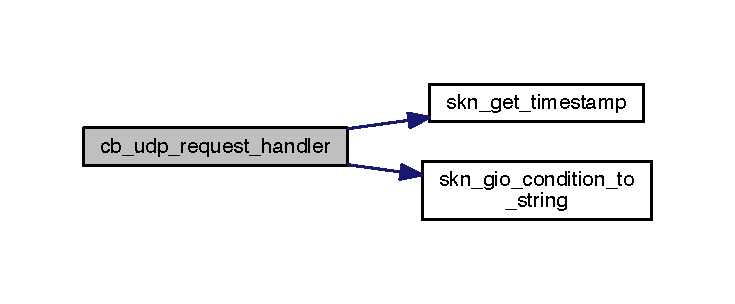
\includegraphics[width=350pt]{cmd_d_s_8c_a49f1fa41c6c2b72cbffa3e0399b12ea7_cgraph}
\end{center}
\end{figure}




Here is the caller graph for this function\+:
\nopagebreak
\begin{figure}[H]
\begin{center}
\leavevmode
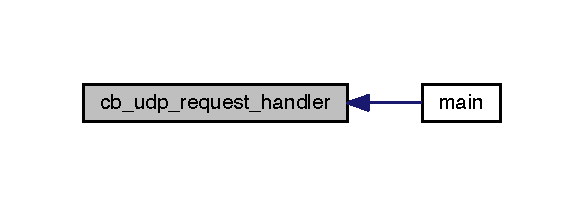
\includegraphics[width=280pt]{cmd_d_s_8c_a49f1fa41c6c2b72cbffa3e0399b12ea7_icgraph}
\end{center}
\end{figure}


\hypertarget{cmd_d_s_8c_a76ad4de5945cff6e20dbeff46bda868b}{}\index{cmd\+D\+S.\+c@{cmd\+D\+S.\+c}!cb\+\_\+unix\+\_\+signal\+\_\+handler@{cb\+\_\+unix\+\_\+signal\+\_\+handler}}
\index{cb\+\_\+unix\+\_\+signal\+\_\+handler@{cb\+\_\+unix\+\_\+signal\+\_\+handler}!cmd\+D\+S.\+c@{cmd\+D\+S.\+c}}
\subsubsection[{cb\+\_\+unix\+\_\+signal\+\_\+handler(\+P\+U\+Signal\+Data psig)}]{\setlength{\rightskip}{0pt plus 5cm}static gboolean cb\+\_\+unix\+\_\+signal\+\_\+handler (
\begin{DoxyParamCaption}
\item[{{\bf P\+U\+Signal\+Data}}]{psig}
\end{DoxyParamCaption}
)\hspace{0.3cm}{\ttfamily [static]}}\label{cmd_d_s_8c_a76ad4de5945cff6e20dbeff46bda868b}


Definition at line 307 of file cmd\+D\+S.\+c.



References \+\_\+signal\+Data\+::loop, and \+\_\+signal\+Data\+::signal\+Name.



Referenced by main().


\begin{DoxyCode}
307                                                           \{
308     g\_message(\textcolor{stringliteral}{"DisplayService::cb\_unix\_signal\_handler() %s Unix Signal Received => Shutdown Initiated!\(\backslash\)n"}, 
      psig->\hyperlink{struct__signal_data_a6b2ce59a22a4ccc54e1d7a54e641d08f}{signalName});
309     g\_main\_loop\_quit(psig->\hyperlink{struct__signal_data_ae85864980ae30c1878e7149c26442544}{loop});
310     \textcolor{keywordflow}{return} ( G\_SOURCE\_REMOVE );
311 \}
\end{DoxyCode}


Here is the caller graph for this function\+:
\nopagebreak
\begin{figure}[H]
\begin{center}
\leavevmode
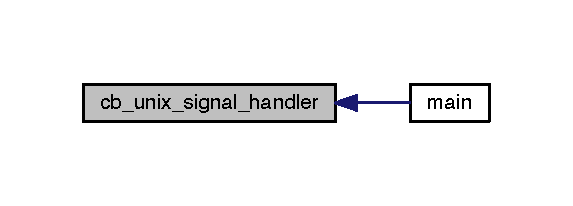
\includegraphics[width=275pt]{cmd_d_s_8c_a76ad4de5945cff6e20dbeff46bda868b_icgraph}
\end{center}
\end{figure}


\hypertarget{cmd_d_s_8c_a3c04138a5bfe5d72780bb7e82a18e627}{}\index{cmd\+D\+S.\+c@{cmd\+D\+S.\+c}!main@{main}}
\index{main@{main}!cmd\+D\+S.\+c@{cmd\+D\+S.\+c}}
\subsubsection[{main(int argc, char $\ast$$\ast$argv)}]{\setlength{\rightskip}{0pt plus 5cm}int main (
\begin{DoxyParamCaption}
\item[{int}]{argc, }
\item[{char $\ast$$\ast$}]{argv}
\end{DoxyParamCaption}
)}\label{cmd_d_s_8c_a3c04138a5bfe5d72780bb7e82a18e627}


Definition at line 632 of file cmd\+D\+S.\+c.



References cb\+\_\+udp\+\_\+broadcast\+\_\+response\+\_\+handler(), cb\+\_\+udp\+\_\+request\+\_\+handler(), cb\+\_\+unix\+\_\+signal\+\_\+handler(), \+\_\+control\+Data\+::ch\+\_\+intf\+Name, \+\_\+control\+Data\+::ch\+\_\+this\+\_\+ip, F\+A\+L\+S\+E, G\+\_\+\+O\+P\+T\+I\+O\+N\+\_\+\+F\+L\+A\+G\+\_\+\+N\+O\+N\+E, \+\_\+control\+Data\+::gb\+Sock, \+\_\+control\+Data\+::g\+Source\+Id, \+\_\+control\+Data\+::g\+U\+D\+P\+Port, \+\_\+signal\+Data\+::loop, \+\_\+control\+Data\+::loop, \+\_\+control\+Data\+::pch\+\_\+service\+\_\+name, \+\_\+control\+Data\+::resolver, \+\_\+signal\+Data\+::signal\+Name, skn\+\_\+get\+\_\+default\+\_\+interface\+\_\+name\+\_\+and\+\_\+ipv4\+\_\+address(), skn\+\_\+udp\+\_\+network\+\_\+broadcast\+\_\+all\+\_\+interfaces(), T\+R\+U\+E, U\+D\+P\+\_\+\+B\+R\+O\+A\+D\+C\+A\+S\+T\+\_\+\+P\+O\+R\+T, and U\+D\+P\+\_\+\+C\+O\+M\+M\+\_\+\+P\+O\+R\+T.


\begin{DoxyCode}
632                                 \{
633 
634     GError *error = NULL;
635     GSocket *gSock = NULL;
636     GSocketAddress *gsAddr = NULL;
637     GInetAddress *anyAddr = NULL;
638     GSource * gSource = NULL;
639     GSocketAddress *gbAddr = NULL;
640     GSource * gBroadSource = NULL;
641     guint gSourceId = 0;
642     \hyperlink{struct__control_data}{ControlData} cData;
643     \hyperlink{struct__ip_broadcast_array}{PIPBroadcastArray} paB = NULL;
644 
645     \hyperlink{struct__signal_data}{USignalData} sigTerm;
646     \hyperlink{struct__signal_data}{USignalData} sigInt;
647     \hyperlink{struct__signal_data}{USignalData} sigHup;
648 
649     guint gUDPPort = 0;
650 
651     GOptionContext *gOptions = NULL;
652     GOptionEntry pgmOptions[] = \{
653        \{\textcolor{stringliteral}{"service-name"}, \textcolor{charliteral}{'a'}, \hyperlink{cmd_d_s_8c_a8e8475ded7103e72515667b568ed64c7}{G\_OPTION\_FLAG\_NONE}, G\_OPTION\_ARG\_STRING, &cData.
      \hyperlink{struct__control_data_a2197fd3d9315510193866dbedbd3cc8b}{pch\_service\_name}, \textcolor{stringliteral}{"Alternate Service Name"}, \textcolor{stringliteral}{"cmdline\_display\_service"}\},
654        \{\textcolor{stringliteral}{"udp\_port\_number"}, \textcolor{charliteral}{'p'}, \hyperlink{cmd_d_s_8c_a8e8475ded7103e72515667b568ed64c7}{G\_OPTION\_FLAG\_NONE}, G\_OPTION\_ARG\_INT, &gUDPPort, \textcolor{stringliteral}{"UDP
       Port Number to listen on."}, \textcolor{stringliteral}{"port number defaults to 48029"}\},
655        \{NULL\}
656     \};
657 
658     cData.\hyperlink{struct__control_data_a2197fd3d9315510193866dbedbd3cc8b}{pch\_service\_name} = NULL;
659 
660     gOptions = g\_option\_context\_new (\textcolor{stringliteral}{"UDP message display service for IOT."});
661     g\_option\_context\_add\_main\_entries (gOptions, pgmOptions, NULL);
662 
663     g\_option\_context\_parse (gOptions, &argc, &argv, &error);
664     \textcolor{keywordflow}{if} (error != NULL) \{
665         g\_error(\textcolor{stringliteral}{"g\_option\_context\_parse() => %s"}, error->message);
666         g\_clear\_error(&error);
667         exit(EXIT\_FAILURE);
668     \}
669     g\_option\_context\_free(gOptions);
670 
671     \textcolor{keywordflow}{if} (gUDPPort == 0) \{
672         gUDPPort = cData.\hyperlink{struct__control_data_a78b36762a9d85d027fc5e41576ade4f7}{gUDPPort} = \hyperlink{cmd_d_s_8c_a88c441c906325a3b6b2738e3218e401f}{UDP\_COMM\_PORT};
673     \} \textcolor{keywordflow}{else} \{
674         cData.\hyperlink{struct__control_data_a78b36762a9d85d027fc5e41576ade4f7}{gUDPPort} = gUDPPort;
675     \}
676     \textcolor{keywordflow}{if} (NULL == cData.\hyperlink{struct__control_data_a2197fd3d9315510193866dbedbd3cc8b}{pch\_service\_name}) \{
677         cData.\hyperlink{struct__control_data_a2197fd3d9315510193866dbedbd3cc8b}{pch\_service\_name} = \textcolor{stringliteral}{"cmdline\_display\_service"};
678     \}
679 
680 
681     paB = \hyperlink{cmd_d_s_8c_a72be87baa67e532c78af054acf935d6c}{skn\_get\_default\_interface\_name\_and\_ipv4\_address}((\textcolor{keywordtype}{
      char} *)&cData.\hyperlink{struct__control_data_adac6cf5482e4bbabb442f8ab27e4bc62}{ch\_intfName}, (\textcolor{keywordtype}{char} *)&cData.\hyperlink{struct__control_data_ac48fc4263dd4a6bad484b93fbf1ffe1b}{ch\_this\_ip});
682     \textcolor{keywordflow}{if} (NULL == paB) \{
683         g\_error(\textcolor{stringliteral}{"skn\_skn\_get\_default\_interface\_name\_and\_ipv4\_address() => Unable to discover network
       interface or non-available."});
684         exit(EXIT\_FAILURE);
685     \}
686 
687     sigHup.\hyperlink{struct__signal_data_ae85864980ae30c1878e7149c26442544}{loop} = sigTerm.\hyperlink{struct__signal_data_ae85864980ae30c1878e7149c26442544}{loop} = sigInt.\hyperlink{struct__signal_data_ae85864980ae30c1878e7149c26442544}{loop} = cData.\hyperlink{struct__control_data_ae1b70bafbd5eb568c6ca339664959216}{loop} =  g\_main\_loop\_new(NULL, 
      \hyperlink{skn__common__headers_8h_aa93f0eb578d23995850d61f7d61c55c1}{FALSE});
688     sigTerm.\hyperlink{struct__signal_data_a6b2ce59a22a4ccc54e1d7a54e641d08f}{signalName} = \textcolor{stringliteral}{"SIGTERM"};
689     sigInt.\hyperlink{struct__signal_data_a6b2ce59a22a4ccc54e1d7a54e641d08f}{signalName} = \textcolor{stringliteral}{"SIGINT"};
690     sigHup.\hyperlink{struct__signal_data_a6b2ce59a22a4ccc54e1d7a54e641d08f}{signalName} = \textcolor{stringliteral}{"SIGHUP"};
691 
692     cData.\hyperlink{struct__control_data_afe33a7083e1ecc9ba50a69644ed4a753}{resolver} = g\_resolver\_get\_default();
693 
694     gSock = g\_socket\_new(G\_SOCKET\_FAMILY\_IPV4, G\_SOCKET\_TYPE\_DATAGRAM, G\_SOCKET\_PROTOCOL\_UDP, &error);
695     \textcolor{keywordflow}{if} (error != NULL) \{
696         g\_error(\textcolor{stringliteral}{"g\_socket\_new() => %s"}, error->message);
697         g\_clear\_error(&error);
698         exit(EXIT\_FAILURE);
699     \}
700 
701     anyAddr = g\_inet\_address\_new\_any(G\_SOCKET\_FAMILY\_IPV4);
702     gsAddr = g\_inet\_socket\_address\_new(anyAddr, gUDPPort);
703 
704     g\_socket\_bind(gSock, gsAddr, \hyperlink{skn__common__headers_8h_aa8cecfc5c5c054d2875c03e77b7be15d}{TRUE}, &error);
705     \textcolor{keywordflow}{if} (error != NULL) \{
706         g\_error(\textcolor{stringliteral}{"g\_socket\_bind() => %s"}, error->message);
707         g\_clear\_error(&error);
708         exit(EXIT\_FAILURE);
709     \}
710 
711     \textcolor{comment}{/*}
712 \textcolor{comment}{     * Create broadcast UDP Socket for receiving messages */}
713     cData.\hyperlink{struct__control_data_a3023250e01849cb311a7207746a3b64e}{gbSock} = g\_socket\_new(G\_SOCKET\_FAMILY\_IPV4, G\_SOCKET\_TYPE\_DATAGRAM, G\_SOCKET\_PROTOCOL\_UDP, 
      &error);
714     \textcolor{keywordflow}{if} (error != NULL) \{
715         g\_error(\textcolor{stringliteral}{"g\_socket\_new(broadcast) => %s"}, error->message);
716         g\_clear\_error(&error);
717         exit(EXIT\_FAILURE);
718     \}
719     g\_socket\_set\_broadcast(cData.\hyperlink{struct__control_data_a3023250e01849cb311a7207746a3b64e}{gbSock}, \hyperlink{skn__common__headers_8h_aa8cecfc5c5c054d2875c03e77b7be15d}{TRUE});
720 
721     gbAddr = g\_inet\_socket\_address\_new(anyAddr, \hyperlink{cmd_d_s_8c_a76bd5a574aad0fa67de6c9804853f191}{UDP\_BROADCAST\_PORT});
722         g\_object\_unref(anyAddr);
723 
724     g\_socket\_bind(cData.\hyperlink{struct__control_data_a3023250e01849cb311a7207746a3b64e}{gbSock}, gbAddr, \hyperlink{skn__common__headers_8h_aa8cecfc5c5c054d2875c03e77b7be15d}{TRUE}, &error);
725     \textcolor{keywordflow}{if} (error != NULL) \{
726         g\_error(\textcolor{stringliteral}{"g\_socket\_bind() => %s"}, error->message);
727         g\_clear\_error(&error);
728         exit(EXIT\_FAILURE);
729     \}
730 
731     \textcolor{comment}{/*}
732 \textcolor{comment}{     * Create and Add socket to gmain loop for service (i.e. polling socket)   */}
733     gSource = g\_socket\_create\_source (gSock, G\_IO\_IN, NULL);
734         g\_source\_set\_callback (gSource, (GSourceFunc) \hyperlink{cmd_d_s_8c_a49f1fa41c6c2b72cbffa3e0399b12ea7}{cb\_udp\_request\_handler}, &cData,
       NULL); \textcolor{comment}{// its really a GSocketSourceFunc}
735         cData.\hyperlink{struct__control_data_a719187f5c3c94da5aa08616db7820b98}{gSourceId} = gSourceId = g\_source\_attach (gSource, NULL);
736 
737     gBroadSource = g\_socket\_create\_source(cData.\hyperlink{struct__control_data_a3023250e01849cb311a7207746a3b64e}{gbSock}, G\_IO\_IN, NULL);
738         g\_source\_ref(gBroadSource);
739         g\_source\_set\_callback (gBroadSource, (GSourceFunc) 
      \hyperlink{cmd_d_s_8c_a385b710fd30ba190b3b96e814424ff80}{cb\_udp\_broadcast\_response\_handler}, &cData, NULL); \textcolor{comment}{// its really a
       GSocketSourceFunc}
740         g\_source\_attach (gBroadSource, NULL);
741 
742     \textcolor{comment}{/*}
743 \textcolor{comment}{     * Handle ctrl-break and kill signals cleanly */}
744     g\_unix\_signal\_add (SIGINT, (GSourceFunc) \hyperlink{cmd_d_s_8c_a76ad4de5945cff6e20dbeff46bda868b}{cb\_unix\_signal\_handler}, &sigInt); \textcolor{comment}{//
       SIGINT signal (Ctrl+C)}
745     g\_unix\_signal\_add (SIGHUP, (GSourceFunc) \hyperlink{cmd_d_s_8c_a76ad4de5945cff6e20dbeff46bda868b}{cb\_unix\_signal\_handler}, &sigHup);
746     g\_unix\_signal\_add (SIGTERM,(GSourceFunc) \hyperlink{cmd_d_s_8c_a76ad4de5945cff6e20dbeff46bda868b}{cb\_unix\_signal\_handler}, &sigTerm);
747 
748 
749     \textcolor{comment}{/*}
750 \textcolor{comment}{     * Broadcast Registry Request: 10.100.1.255 */}
751     \textcolor{keywordflow}{if} ( \hyperlink{cmd_d_s_8c_af376243f65a3fd761050836d1293b0d9}{skn\_udp\_network\_broadcast\_all\_interfaces}(cData.
      \hyperlink{struct__control_data_a3023250e01849cb311a7207746a3b64e}{gbSock}, paB) ) \{
752         g\_message(\textcolor{stringliteral}{"cmdDS: Ready to do Good, on %s:%s:%d...\(\backslash\)n"}, cData.\hyperlink{struct__control_data_adac6cf5482e4bbabb442f8ab27e4bc62}{ch\_intfName}, cData.
      \hyperlink{struct__control_data_ac48fc4263dd4a6bad484b93fbf1ffe1b}{ch\_this\_ip}, gUDPPort);
753 
754         g\_main\_loop\_run(cData.\hyperlink{struct__control_data_ae1b70bafbd5eb568c6ca339664959216}{loop});
755     \}
756 
757     g\_main\_loop\_unref(cData.\hyperlink{struct__control_data_ae1b70bafbd5eb568c6ca339664959216}{loop});
758 
759     g\_source\_unref(gBroadSource);
760     g\_source\_unref(gSource);
761     g\_object\_unref(cData.\hyperlink{struct__control_data_a3023250e01849cb311a7207746a3b64e}{gbSock});
762     g\_object\_unref(gSock);
763     g\_object\_unref(gbAddr);
764     g\_object\_unref(gsAddr);
765     g\_object\_unref(cData.\hyperlink{struct__control_data_afe33a7083e1ecc9ba50a69644ed4a753}{resolver});
766 
767     g\_message(\textcolor{stringliteral}{"cmdDS: normal shutdown..."});
768 
769     exit(EXIT\_SUCCESS);
770 \}
\end{DoxyCode}


Here is the call graph for this function\+:
\nopagebreak
\begin{figure}[H]
\begin{center}
\leavevmode
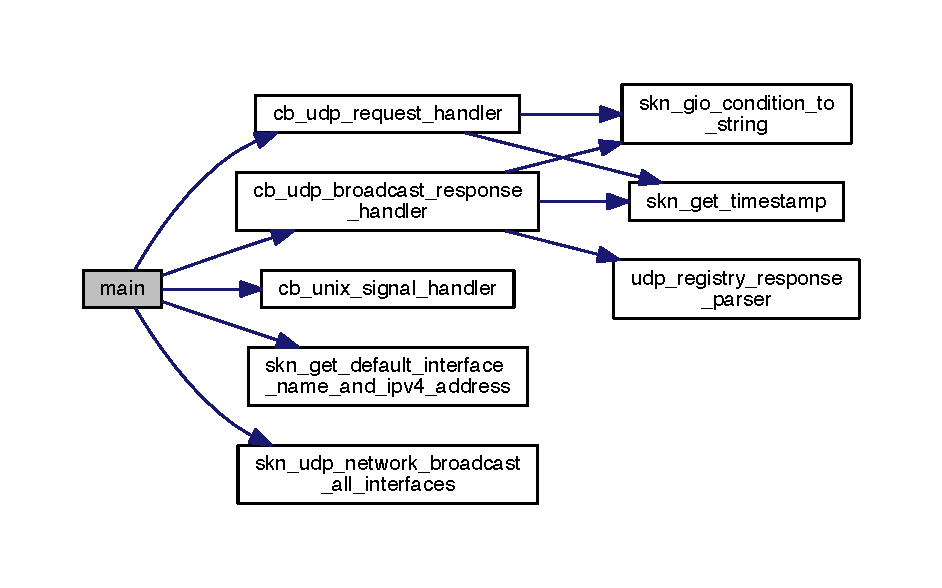
\includegraphics[width=350pt]{cmd_d_s_8c_a3c04138a5bfe5d72780bb7e82a18e627_cgraph}
\end{center}
\end{figure}


\hypertarget{cmd_d_s_8c_a0dfc1a6916909805dc7fd2d8c471e0e3}{}\index{cmd\+D\+S.\+c@{cmd\+D\+S.\+c}!skn\+\_\+get\+\_\+broadcast\+\_\+ip\+\_\+array@{skn\+\_\+get\+\_\+broadcast\+\_\+ip\+\_\+array}}
\index{skn\+\_\+get\+\_\+broadcast\+\_\+ip\+\_\+array@{skn\+\_\+get\+\_\+broadcast\+\_\+ip\+\_\+array}!cmd\+D\+S.\+c@{cmd\+D\+S.\+c}}
\subsubsection[{skn\+\_\+get\+\_\+broadcast\+\_\+ip\+\_\+array(\+P\+I\+P\+Broadcast\+Array pa\+B)}]{\setlength{\rightskip}{0pt plus 5cm}gint skn\+\_\+get\+\_\+broadcast\+\_\+ip\+\_\+array (
\begin{DoxyParamCaption}
\item[{{\bf P\+I\+P\+Broadcast\+Array}}]{pa\+B}
\end{DoxyParamCaption}
)}\label{cmd_d_s_8c_a0dfc1a6916909805dc7fd2d8c471e0e3}
Collect I\+P and Broadcast Addresses for this machine


\begin{DoxyItemize}
\item Affects the P\+I\+P\+Broadcast\+Array
\item Return -\/1 on error, or count of interfaces
\item contains this ip\+Address in pa\+B-\/$>$ip\+Addr\+Str\mbox{[}pa\+B-\/$>$default\+Index\mbox{]} 
\end{DoxyItemize}

Definition at line 170 of file cmd\+D\+S.\+c.



References A\+R\+Y\+\_\+\+M\+A\+X\+\_\+\+I\+N\+T\+F, \+\_\+ip\+Broadcast\+Array\+::broad\+Addr\+Str, \+\_\+ip\+Broadcast\+Array\+::cb\+Name, \+\_\+ip\+Broadcast\+Array\+::ch\+Default\+Intf\+Name, \+\_\+ip\+Broadcast\+Array\+::count, \+\_\+ip\+Broadcast\+Array\+::default\+Index, \+\_\+ip\+Broadcast\+Array\+::if\+Name\+Str, \+\_\+ip\+Broadcast\+Array\+::ip\+Addr\+Str, \+\_\+ip\+Broadcast\+Array\+::mask\+Addr\+Str, P\+L\+A\+T\+F\+O\+R\+M\+\_\+\+E\+R\+R\+O\+R, skn\+\_\+get\+\_\+default\+\_\+interface\+\_\+name(), and S\+Z\+\_\+\+C\+H\+A\+R\+\_\+\+B\+U\+F\+F.



Referenced by skn\+\_\+get\+\_\+default\+\_\+interface\+\_\+name\+\_\+and\+\_\+ipv4\+\_\+address().


\begin{DoxyCode}
170                                                        \{
171     \textcolor{keyword}{struct }ifaddrs * ifap;
172     \textcolor{keyword}{struct }ifaddrs * p;
173     gint rc = 0;
174 
175     memset(paB, 0, \textcolor{keyword}{sizeof}(\hyperlink{struct__ip_broadcast_array}{IPBroadcastArray}));
176     paB->\hyperlink{struct__ip_broadcast_array_a971377a4c995292b8bd908f185cfc844}{count} = 0;
177     paB->\hyperlink{struct__ip_broadcast_array_a5822ff77ae9f31bd3b4298d463c02f1f}{defaultIndex} = 0;
178     strcpy(paB->\hyperlink{struct__ip_broadcast_array_a0f592bd31dcc3ce00a349f04ff6bd1ba}{cbName}, \textcolor{stringliteral}{"IPBroadcastArray"});
179 
180     rc = \hyperlink{cmd_d_s_8c_afc164e6efc7bdcdbacba97ba6f6c2a19}{skn\_get\_default\_interface\_name}(paB->
      \hyperlink{struct__ip_broadcast_array_a06dab8742df19b5aec8538842617778d}{chDefaultIntfName});
181     \textcolor{keywordflow}{if} (rc == EXIT\_FAILURE) \{ \textcolor{comment}{// Alternate method for Mac: 'route -n -A inet'}
182         g\_warning(\textcolor{stringliteral}{"[REGISTRY] No Default Network Interfaces Found!."});
183         paB->\hyperlink{struct__ip_broadcast_array_a06dab8742df19b5aec8538842617778d}{chDefaultIntfName}[0] = 0;
184     \}
185     rc = getifaddrs(&ifap);
186     \textcolor{keywordflow}{if} (rc != 0) \{
187         g\_warning(\textcolor{stringliteral}{"[REGISTRY] No Network Interfaces Found at All ! %d:%d:%s"}, rc, errno, strerror(errno) );
188         \textcolor{keywordflow}{return} (\hyperlink{cmd_d_s_8c_a12efd06fda89d6826f820e75148d8fd7}{PLATFORM\_ERROR});
189     \}
190     p = ifap;
191 
192     \textcolor{keywordflow}{while} (p && (paB->\hyperlink{struct__ip_broadcast_array_a971377a4c995292b8bd908f185cfc844}{count} < \hyperlink{cmd_d_s_8c_a00b19837422a3b13d82b9a525e92ef51}{ARY\_MAX\_INTF})) \{
193         \textcolor{keywordflow}{if} (p->ifa\_addr != NULL && p->ifa\_addr->sa\_family == AF\_INET && ((p->ifa\_flags & IFF\_BROADCAST) > 0
      )) \{
194 
195             inet\_ntop(p->ifa\_addr->sa\_family, &((\textcolor{keyword}{struct} sockaddr\_in *) p->ifa\_addr)->sin\_addr, paB->
      \hyperlink{struct__ip_broadcast_array_a96891ccc707337890b2a166e3ef3a8e1}{ipAddrStr}[paB->\hyperlink{struct__ip_broadcast_array_a971377a4c995292b8bd908f185cfc844}{count}], (\hyperlink{cmd_d_s_8c_a8d2978ad614b0de81c60483e706d9306}{SZ\_CHAR\_BUFF} - 1));
196             inet\_ntop(p->ifa\_addr->sa\_family, &((\textcolor{keyword}{struct} sockaddr\_in *) p->ifa\_netmask)->sin\_addr, paB->
      \hyperlink{struct__ip_broadcast_array_a9241c1fbfb22a3ecfe4777863a063eb3}{maskAddrStr}[paB->\hyperlink{struct__ip_broadcast_array_a971377a4c995292b8bd908f185cfc844}{count}], (\hyperlink{cmd_d_s_8c_a8d2978ad614b0de81c60483e706d9306}{SZ\_CHAR\_BUFF} - 1));
197             inet\_ntop(p->ifa\_addr->sa\_family, &((\textcolor{keyword}{struct} sockaddr\_in *) p->ifa\_broadaddr)->sin\_addr, paB->
      \hyperlink{struct__ip_broadcast_array_af40943e174ba847fa0218cfa6051e277}{broadAddrStr}[paB->\hyperlink{struct__ip_broadcast_array_a971377a4c995292b8bd908f185cfc844}{count}], (\hyperlink{cmd_d_s_8c_a8d2978ad614b0de81c60483e706d9306}{SZ\_CHAR\_BUFF} - 1));
198 
199             strncpy(paB->\hyperlink{struct__ip_broadcast_array_a193b90f271c061e8bf1593bab6a182c9}{ifNameStr}[paB->\hyperlink{struct__ip_broadcast_array_a971377a4c995292b8bd908f185cfc844}{count}], p->ifa\_name, (
      \hyperlink{cmd_d_s_8c_a8d2978ad614b0de81c60483e706d9306}{SZ\_CHAR\_BUFF} -1));
200 
201             \textcolor{comment}{/* Take match as the default */}
202             \textcolor{keywordflow}{if} (strcmp(paB->\hyperlink{struct__ip_broadcast_array_a06dab8742df19b5aec8538842617778d}{chDefaultIntfName}, p->ifa\_name) == 0) \{
203                 paB->\hyperlink{struct__ip_broadcast_array_a5822ff77ae9f31bd3b4298d463c02f1f}{defaultIndex} = paB->\hyperlink{struct__ip_broadcast_array_a971377a4c995292b8bd908f185cfc844}{count};
204             \}
205 
206             paB->\hyperlink{struct__ip_broadcast_array_a971377a4c995292b8bd908f185cfc844}{count}++;
207         \}
208         p = p->ifa\_next;
209     \} \textcolor{comment}{// end while}
210     freeifaddrs(ifap);
211 
212     \textcolor{keywordflow}{return} (paB->\hyperlink{struct__ip_broadcast_array_a971377a4c995292b8bd908f185cfc844}{count});
213 \}
\end{DoxyCode}


Here is the call graph for this function\+:
\nopagebreak
\begin{figure}[H]
\begin{center}
\leavevmode
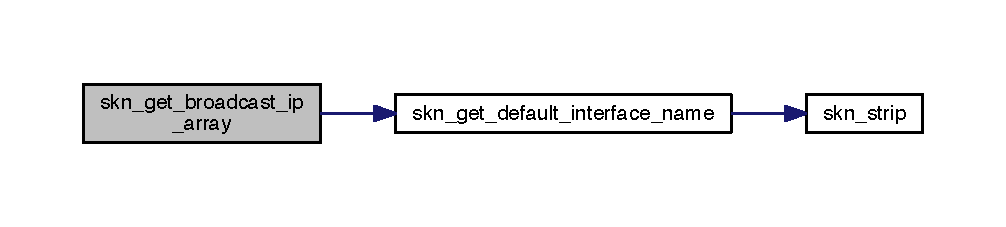
\includegraphics[width=350pt]{cmd_d_s_8c_a0dfc1a6916909805dc7fd2d8c471e0e3_cgraph}
\end{center}
\end{figure}




Here is the caller graph for this function\+:
\nopagebreak
\begin{figure}[H]
\begin{center}
\leavevmode
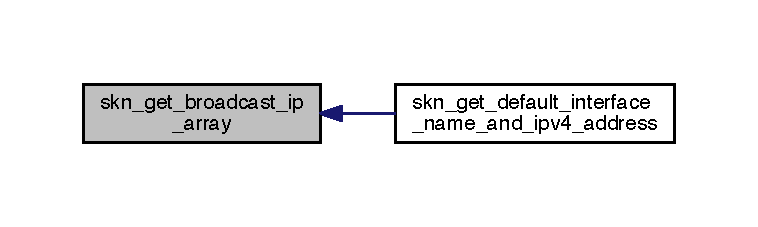
\includegraphics[width=350pt]{cmd_d_s_8c_a0dfc1a6916909805dc7fd2d8c471e0e3_icgraph}
\end{center}
\end{figure}


\hypertarget{cmd_d_s_8c_afc164e6efc7bdcdbacba97ba6f6c2a19}{}\index{cmd\+D\+S.\+c@{cmd\+D\+S.\+c}!skn\+\_\+get\+\_\+default\+\_\+interface\+\_\+name@{skn\+\_\+get\+\_\+default\+\_\+interface\+\_\+name}}
\index{skn\+\_\+get\+\_\+default\+\_\+interface\+\_\+name@{skn\+\_\+get\+\_\+default\+\_\+interface\+\_\+name}!cmd\+D\+S.\+c@{cmd\+D\+S.\+c}}
\subsubsection[{skn\+\_\+get\+\_\+default\+\_\+interface\+\_\+name(char $\ast$pch\+Default\+Interface\+Name)}]{\setlength{\rightskip}{0pt plus 5cm}gint skn\+\_\+get\+\_\+default\+\_\+interface\+\_\+name (
\begin{DoxyParamCaption}
\item[{char $\ast$}]{pch\+Default\+Interface\+Name}
\end{DoxyParamCaption}
)}\label{cmd_d_s_8c_afc164e6efc7bdcdbacba97ba6f6c2a19}
Retrieves default internet interface name into param
\begin{DoxyItemize}
\item absolute best way to do this, but not supported on Darwin(i.\+e O\+S\+X) return E\+X\+I\+T\+\_\+\+S\+U\+C\+C\+E\+S\+S or E\+X\+I\+T\+\_\+\+F\+A\+I\+L\+U\+R\+E
\end{DoxyItemize}

\mbox{[}jscott O\+S\+X\mbox{]}\$ route -\/n get 0.\+0.\+0.\+0 route to\+: default destination\+: default mask\+: default gateway\+: 10.\+21.\+1.\+254 interface\+: en3 flags\+: $<$U\+P,G\+A\+T\+E\+W\+A\+Y,D\+O\+N\+E,S\+T\+A\+T\+I\+C,P\+R\+C\+L\+O\+N\+I\+N\+G$>$ recvpipe sendpipe ssthresh rtt,msec rttvar hopcount mtu expire 0 0 0 0 0 0 1500 0 

Definition at line 231 of file cmd\+D\+S.\+c.



References skn\+\_\+strip(), and S\+Z\+\_\+\+I\+N\+F\+O\+\_\+\+B\+U\+F\+F.



Referenced by skn\+\_\+get\+\_\+broadcast\+\_\+ip\+\_\+array().


\begin{DoxyCode}
231                                                                    \{
232     FILE *f\_route;
233     \textcolor{keywordtype}{char} line[\hyperlink{cmd_d_s_8c_a442d5e93bd9c9d8eb4532aba62b5f86c}{SZ\_INFO\_BUFF}], *dRoute = NULL, *iName = NULL;
234 
235     f\_route = fopen(\textcolor{stringliteral}{"/proc/net/route"}, \textcolor{stringliteral}{"r"});
236     \textcolor{keywordflow}{if} (f\_route != NULL) \{
237         \textcolor{keywordflow}{while} (fgets(line, \hyperlink{cmd_d_s_8c_a442d5e93bd9c9d8eb4532aba62b5f86c}{SZ\_INFO\_BUFF} - 1, f\_route)) \{
238             iName = strtok(line, \textcolor{stringliteral}{"\(\backslash\)t"});
239             dRoute = strtok(NULL, \textcolor{stringliteral}{"\(\backslash\)t"});
240 
241             \textcolor{keywordflow}{if} (iName != NULL && dRoute != NULL) \{
242                 \textcolor{keywordflow}{if} (strcmp(dRoute, \textcolor{stringliteral}{"00000000"}) == 0) \{
243                     strncpy(pchDefaultInterfaceName, iName, (\hyperlink{cmd_d_s_8c_a442d5e93bd9c9d8eb4532aba62b5f86c}{SZ\_INFO\_BUFF} - 1));
244                     \textcolor{keywordflow}{break};
245                 \}
246             \}
247         \}
248         fclose(f\_route);
249 
250         \textcolor{keywordflow}{return} (EXIT\_SUCCESS);
251     \}
252    g\_print(\textcolor{stringliteral}{"[REGISTRY] Opening ProcFs for RouteInfo Failed: %d:%s, Alternate method will be attempted."}, 
      errno, strerror(errno));
253 
254     f\_route = popen(\textcolor{stringliteral}{"route -n get 0.0.0.0"}, \textcolor{stringliteral}{"r"}); \textcolor{comment}{// for linux 'route -n -A inet', with interface at
       line\_word[7]}
255     \textcolor{keywordflow}{if} (f\_route != NULL) \{
256         \textcolor{keywordflow}{while} (fgets(line, \hyperlink{cmd_d_s_8c_a442d5e93bd9c9d8eb4532aba62b5f86c}{SZ\_INFO\_BUFF} - 1, f\_route)) \{
257             dRoute = strtok(line, \textcolor{stringliteral}{":"});
258             iName = strtok(NULL, \textcolor{stringliteral}{"\(\backslash\)n"});
259             \textcolor{keywordflow}{if} (strcmp(\hyperlink{cmd_d_s_8c_a5acaf42e0ff80bd0de38c490576e9f85}{skn\_strip}(dRoute), \textcolor{stringliteral}{"interface"}) == 0) \{
260                 strncpy(pchDefaultInterfaceName, \hyperlink{cmd_d_s_8c_a5acaf42e0ff80bd0de38c490576e9f85}{skn\_strip}(iName), (
      \hyperlink{cmd_d_s_8c_a442d5e93bd9c9d8eb4532aba62b5f86c}{SZ\_INFO\_BUFF} - 1));
261                 \textcolor{keywordflow}{break};
262             \}
263         \}
264         fclose(f\_route);
265 
266         \textcolor{keywordflow}{return} (EXIT\_SUCCESS);
267     \} \textcolor{keywordflow}{else} \{
268         g\_warning(\textcolor{stringliteral}{"[REGISTRY] Alternate method to get RouteInfo Failed: %d:%s"}, errno, strerror(errno));
269         \textcolor{keywordflow}{return} (EXIT\_FAILURE);
270     \}
271 
272 \}
\end{DoxyCode}


Here is the call graph for this function\+:
\nopagebreak
\begin{figure}[H]
\begin{center}
\leavevmode
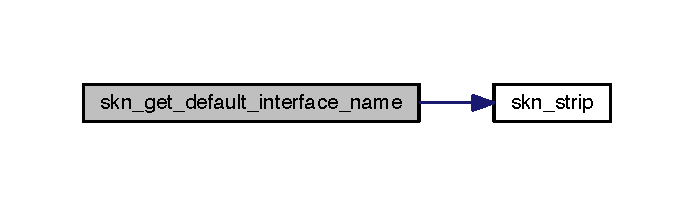
\includegraphics[width=333pt]{cmd_d_s_8c_afc164e6efc7bdcdbacba97ba6f6c2a19_cgraph}
\end{center}
\end{figure}




Here is the caller graph for this function\+:
\nopagebreak
\begin{figure}[H]
\begin{center}
\leavevmode
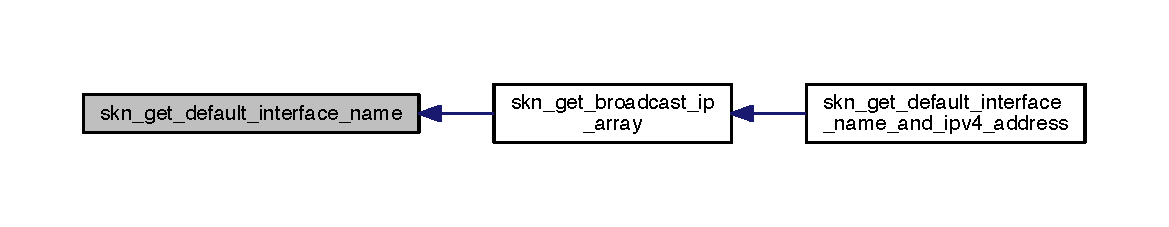
\includegraphics[width=350pt]{cmd_d_s_8c_afc164e6efc7bdcdbacba97ba6f6c2a19_icgraph}
\end{center}
\end{figure}


\hypertarget{cmd_d_s_8c_a72be87baa67e532c78af054acf935d6c}{}\index{cmd\+D\+S.\+c@{cmd\+D\+S.\+c}!skn\+\_\+get\+\_\+default\+\_\+interface\+\_\+name\+\_\+and\+\_\+ipv4\+\_\+address@{skn\+\_\+get\+\_\+default\+\_\+interface\+\_\+name\+\_\+and\+\_\+ipv4\+\_\+address}}
\index{skn\+\_\+get\+\_\+default\+\_\+interface\+\_\+name\+\_\+and\+\_\+ipv4\+\_\+address@{skn\+\_\+get\+\_\+default\+\_\+interface\+\_\+name\+\_\+and\+\_\+ipv4\+\_\+address}!cmd\+D\+S.\+c@{cmd\+D\+S.\+c}}
\subsubsection[{skn\+\_\+get\+\_\+default\+\_\+interface\+\_\+name\+\_\+and\+\_\+ipv4\+\_\+address(char $\ast$intf, char $\ast$ipv4)}]{\setlength{\rightskip}{0pt plus 5cm}{\bf P\+I\+P\+Broadcast\+Array} skn\+\_\+get\+\_\+default\+\_\+interface\+\_\+name\+\_\+and\+\_\+ipv4\+\_\+address (
\begin{DoxyParamCaption}
\item[{char $\ast$}]{intf, }
\item[{char $\ast$}]{ipv4}
\end{DoxyParamCaption}
)}\label{cmd_d_s_8c_a72be87baa67e532c78af054acf935d6c}


Referenced by main().



Here is the caller graph for this function\+:
\nopagebreak
\begin{figure}[H]
\begin{center}
\leavevmode
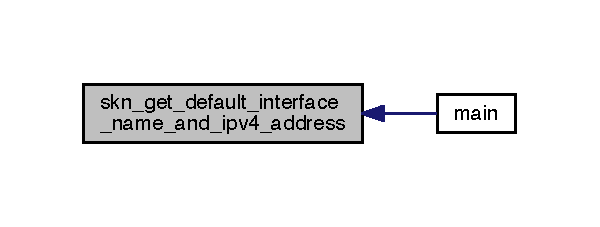
\includegraphics[width=288pt]{cmd_d_s_8c_a72be87baa67e532c78af054acf935d6c_icgraph}
\end{center}
\end{figure}


\hypertarget{cmd_d_s_8c_a4f733621137368e762c5db74a3cec52b}{}\index{cmd\+D\+S.\+c@{cmd\+D\+S.\+c}!skn\+\_\+get\+\_\+default\+\_\+interface\+\_\+name\+\_\+and\+\_\+ipv4\+\_\+address@{skn\+\_\+get\+\_\+default\+\_\+interface\+\_\+name\+\_\+and\+\_\+ipv4\+\_\+address}}
\index{skn\+\_\+get\+\_\+default\+\_\+interface\+\_\+name\+\_\+and\+\_\+ipv4\+\_\+address@{skn\+\_\+get\+\_\+default\+\_\+interface\+\_\+name\+\_\+and\+\_\+ipv4\+\_\+address}!cmd\+D\+S.\+c@{cmd\+D\+S.\+c}}
\subsubsection[{skn\+\_\+get\+\_\+default\+\_\+interface\+\_\+name\+\_\+and\+\_\+ipv4\+\_\+address(gchar $\ast$intf, gchar $\ast$ipv4)}]{\setlength{\rightskip}{0pt plus 5cm}{\bf P\+I\+P\+Broadcast\+Array} skn\+\_\+get\+\_\+default\+\_\+interface\+\_\+name\+\_\+and\+\_\+ipv4\+\_\+address (
\begin{DoxyParamCaption}
\item[{gchar $\ast$}]{intf, }
\item[{gchar $\ast$}]{ipv4}
\end{DoxyParamCaption}
)}\label{cmd_d_s_8c_a4f733621137368e762c5db74a3cec52b}


Definition at line 150 of file cmd\+D\+S.\+c.



References \+\_\+ip\+Broadcast\+Array\+::ch\+Default\+Intf\+Name, \+\_\+ip\+Broadcast\+Array\+::default\+Index, \+\_\+ip\+Broadcast\+Array\+::ip\+Addr\+Str, P\+L\+A\+T\+F\+O\+R\+M\+\_\+\+E\+R\+R\+O\+R, skn\+\_\+get\+\_\+broadcast\+\_\+ip\+\_\+array(), and S\+Z\+\_\+\+C\+H\+A\+R\+\_\+\+B\+U\+F\+F.


\begin{DoxyCode}
150                                                                                               \{
151     \hyperlink{struct__ip_broadcast_array}{PIPBroadcastArray} paB = g\_new0(\hyperlink{struct__ip_broadcast_array}{IPBroadcastArray}, 1);
152 
153     \textcolor{keywordflow}{if} (\hyperlink{cmd_d_s_8c_a0dfc1a6916909805dc7fd2d8c471e0e3}{skn\_get\_broadcast\_ip\_array}(paB) != 
      \hyperlink{cmd_d_s_8c_a12efd06fda89d6826f820e75148d8fd7}{PLATFORM\_ERROR}) \{
154         g\_utf8\_strncpy(intf, paB->\hyperlink{struct__ip_broadcast_array_a06dab8742df19b5aec8538842617778d}{chDefaultIntfName}, 
      \hyperlink{cmd_d_s_8c_a8d2978ad614b0de81c60483e706d9306}{SZ\_CHAR\_BUFF});
155         g\_utf8\_strncpy(ipv4, paB->\hyperlink{struct__ip_broadcast_array_a96891ccc707337890b2a166e3ef3a8e1}{ipAddrStr}[paB->\hyperlink{struct__ip_broadcast_array_a5822ff77ae9f31bd3b4298d463c02f1f}{defaultIndex}], 
      \hyperlink{cmd_d_s_8c_a8d2978ad614b0de81c60483e706d9306}{SZ\_CHAR\_BUFF});
156     \} \textcolor{keywordflow}{else} \{
157         g\_warning(\textcolor{stringliteral}{"[REGISTRY] InterfaceName and Address: unable to access information."});
158         \textcolor{keywordflow}{return}(NULL);
159     \}
160     \textcolor{keywordflow}{return} (paB);
161 \}
\end{DoxyCode}


Here is the call graph for this function\+:
\nopagebreak
\begin{figure}[H]
\begin{center}
\leavevmode
\includegraphics[width=350pt]{cmd_d_s_8c_a4f733621137368e762c5db74a3cec52b_cgraph}
\end{center}
\end{figure}


\hypertarget{cmd_d_s_8c_a6ea2e6ee5c8f0d51a98539842634f217}{}\index{cmd\+D\+S.\+c@{cmd\+D\+S.\+c}!skn\+\_\+get\+\_\+timestamp@{skn\+\_\+get\+\_\+timestamp}}
\index{skn\+\_\+get\+\_\+timestamp@{skn\+\_\+get\+\_\+timestamp}!cmd\+D\+S.\+c@{cmd\+D\+S.\+c}}
\subsubsection[{skn\+\_\+get\+\_\+timestamp()}]{\setlength{\rightskip}{0pt plus 5cm}gchar$\ast$ skn\+\_\+get\+\_\+timestamp (
\begin{DoxyParamCaption}
{}
\end{DoxyParamCaption}
)}\label{cmd_d_s_8c_a6ea2e6ee5c8f0d51a98539842634f217}


Definition at line 312 of file cmd\+D\+S.\+c.



Referenced by cb\+\_\+udp\+\_\+broadcast\+\_\+response\+\_\+handler(), and cb\+\_\+udp\+\_\+request\+\_\+handler().


\begin{DoxyCode}
312                             \{
313     GDateTime   *stamp = g\_date\_time\_new\_now\_local();
314     gchar *response = g\_date\_time\_format(stamp,\textcolor{stringliteral}{"%F.%T"});
315 
316     \textcolor{keywordflow}{return}(response);
317 \}
\end{DoxyCode}


Here is the caller graph for this function\+:
\nopagebreak
\begin{figure}[H]
\begin{center}
\leavevmode
\includegraphics[width=350pt]{cmd_d_s_8c_a6ea2e6ee5c8f0d51a98539842634f217_icgraph}
\end{center}
\end{figure}


\hypertarget{cmd_d_s_8c_a2dcc830aabe5f0cfffb3077fc0cba6a5}{}\index{cmd\+D\+S.\+c@{cmd\+D\+S.\+c}!skn\+\_\+gio\+\_\+condition\+\_\+to\+\_\+string@{skn\+\_\+gio\+\_\+condition\+\_\+to\+\_\+string}}
\index{skn\+\_\+gio\+\_\+condition\+\_\+to\+\_\+string@{skn\+\_\+gio\+\_\+condition\+\_\+to\+\_\+string}!cmd\+D\+S.\+c@{cmd\+D\+S.\+c}}
\subsubsection[{skn\+\_\+gio\+\_\+condition\+\_\+to\+\_\+string(\+G\+I\+O\+Condition condition)}]{\setlength{\rightskip}{0pt plus 5cm}gchar$\ast$ skn\+\_\+gio\+\_\+condition\+\_\+to\+\_\+string (
\begin{DoxyParamCaption}
\item[{G\+I\+O\+Condition}]{condition}
\end{DoxyParamCaption}
)}\label{cmd_d_s_8c_a2dcc830aabe5f0cfffb3077fc0cba6a5}


Definition at line 603 of file cmd\+D\+S.\+c.



Referenced by cb\+\_\+udp\+\_\+broadcast\+\_\+response\+\_\+handler(), and cb\+\_\+udp\+\_\+request\+\_\+handler().


\begin{DoxyCode}
603                                                             \{
604     gchar *value = NULL;
605 
606     \textcolor{keywordflow}{switch}(condition) \{
607         \textcolor{keywordflow}{case} G\_IO\_IN:
608             value = \textcolor{stringliteral}{"There is data to read."};
609             \textcolor{keywordflow}{break};
610         \textcolor{keywordflow}{case} G\_IO\_OUT:
611             value = \textcolor{stringliteral}{"Data can be written (without blocking)."};
612             \textcolor{keywordflow}{break};
613         \textcolor{keywordflow}{case} G\_IO\_PRI:
614             value = \textcolor{stringliteral}{"There is urgent data to read."};
615             \textcolor{keywordflow}{break};
616         \textcolor{keywordflow}{case} G\_IO\_ERR:
617             value = \textcolor{stringliteral}{"Error condition."};
618             \textcolor{keywordflow}{break};
619         \textcolor{keywordflow}{case} G\_IO\_HUP:
620             value = \textcolor{stringliteral}{"Hung up (the connection has been broken, usually for pipes and sockets)."};
621             \textcolor{keywordflow}{break};
622         \textcolor{keywordflow}{case} G\_IO\_NVAL:
623             value = \textcolor{stringliteral}{"Invalid request. The file descriptor is not open."};
624             \textcolor{keywordflow}{break};
625         \textcolor{keywordflow}{default}:
626             value = \textcolor{stringliteral}{"Unknown GIOCondition!"};
627     \}
628 
629     \textcolor{keywordflow}{return} (value);
630 \}
\end{DoxyCode}


Here is the caller graph for this function\+:
\nopagebreak
\begin{figure}[H]
\begin{center}
\leavevmode
\includegraphics[width=350pt]{cmd_d_s_8c_a2dcc830aabe5f0cfffb3077fc0cba6a5_icgraph}
\end{center}
\end{figure}


\hypertarget{cmd_d_s_8c_a5acaf42e0ff80bd0de38c490576e9f85}{}\index{cmd\+D\+S.\+c@{cmd\+D\+S.\+c}!skn\+\_\+strip@{skn\+\_\+strip}}
\index{skn\+\_\+strip@{skn\+\_\+strip}!cmd\+D\+S.\+c@{cmd\+D\+S.\+c}}
\subsubsection[{skn\+\_\+strip(gchar $\ast$alpha)}]{\setlength{\rightskip}{0pt plus 5cm}gchar$\ast$ skn\+\_\+strip (
\begin{DoxyParamCaption}
\item[{gchar $\ast$}]{alpha}
\end{DoxyParamCaption}
)}\label{cmd_d_s_8c_a5acaf42e0ff80bd0de38c490576e9f85}
Remove Trailing and Leading Blanks
\begin{DoxyItemize}
\item caution\+: pointers from argv are readonly and segfault on \textquotesingle{}alpha\mbox{[}end\mbox{]} = 0\textquotesingle{} 
\end{DoxyItemize}

Definition at line 124 of file cmd\+D\+S.\+c.



Referenced by skn\+\_\+get\+\_\+default\+\_\+interface\+\_\+name().


\begin{DoxyCode}
124                                  \{
125     \textcolor{keywordflow}{if} (alpha == NULL || strlen(alpha) < 1)
126         \textcolor{keywordflow}{return}(alpha);
127 
128     \textcolor{keywordtype}{int} len = strlen(alpha);
129     \textcolor{keywordtype}{int} end = len - 1;
130     \textcolor{keywordtype}{int} start = 0;
131 
132     \textcolor{comment}{// use isgraph() or !isspace() vs isalnum() to allow ['|' ';' '%']}
133     \textcolor{keywordflow}{while} ( !g\_unichar\_isgraph(alpha[end]) && end > 0 ) \{ \textcolor{comment}{// remove trailing non-alphanumeric chars}
134         alpha[end--] = 0;
135     \}
136 
137     len = strlen(alpha);
138     \textcolor{keywordflow}{while} ( !g\_unichar\_isalnum(alpha[start]) && start < len ) \{ \textcolor{comment}{// find first non-alpha stricter}
139         start++;
140     \}
141     \textcolor{keywordflow}{if} (start < len && start > 0) \{  \textcolor{comment}{// move in place}
142         end = len - start;
143         memmove(&alpha[0], &alpha[start], end);
144         alpha[end] = 0;
145     \}
146 
147     \textcolor{keywordflow}{return}(alpha);
148 \}
\end{DoxyCode}


Here is the caller graph for this function\+:
\nopagebreak
\begin{figure}[H]
\begin{center}
\leavevmode
\includegraphics[width=350pt]{cmd_d_s_8c_a5acaf42e0ff80bd0de38c490576e9f85_icgraph}
\end{center}
\end{figure}


\hypertarget{cmd_d_s_8c_af376243f65a3fd761050836d1293b0d9}{}\index{cmd\+D\+S.\+c@{cmd\+D\+S.\+c}!skn\+\_\+udp\+\_\+network\+\_\+broadcast\+\_\+all\+\_\+interfaces@{skn\+\_\+udp\+\_\+network\+\_\+broadcast\+\_\+all\+\_\+interfaces}}
\index{skn\+\_\+udp\+\_\+network\+\_\+broadcast\+\_\+all\+\_\+interfaces@{skn\+\_\+udp\+\_\+network\+\_\+broadcast\+\_\+all\+\_\+interfaces}!cmd\+D\+S.\+c@{cmd\+D\+S.\+c}}
\subsubsection[{skn\+\_\+udp\+\_\+network\+\_\+broadcast\+\_\+all\+\_\+interfaces(\+G\+Socket $\ast$g\+Sock, P\+I\+P\+Broadcast\+Array pab)}]{\setlength{\rightskip}{0pt plus 5cm}gboolean skn\+\_\+udp\+\_\+network\+\_\+broadcast\+\_\+all\+\_\+interfaces (
\begin{DoxyParamCaption}
\item[{G\+Socket $\ast$}]{g\+Sock, }
\item[{{\bf P\+I\+P\+Broadcast\+Array}}]{pa\+B}
\end{DoxyParamCaption}
)}\label{cmd_d_s_8c_af376243f65a3fd761050836d1293b0d9}
Send a registry request on the broadcast ip of all interfaces


\begin{DoxyParams}{Parameters}
{\em g\+Sock} & I\+N G\+Lib active/bound socket with broadcast enabled \\
\hline
{\em ch\+\_\+request} & I\+N Greetings message, anytext \\
\hline
{\em ch\+\_\+intf\+Name} & O\+U\+T Default Ethernet Interface Name \\
\hline
{\em ch\+\_\+ip\+Address} & O\+U\+T Default Ethernet I\+P Address \\
\hline
\end{DoxyParams}
\begin{DoxyReturn}{Returns}
true on success, 
\end{DoxyReturn}


Definition at line 282 of file cmd\+D\+S.\+c.



References \+\_\+ip\+Broadcast\+Array\+::broad\+Addr\+Str, \+\_\+ip\+Broadcast\+Array\+::count, \+\_\+ip\+Broadcast\+Array\+::default\+Index, \+\_\+ip\+Broadcast\+Array\+::if\+Name\+Str, \+\_\+ip\+Broadcast\+Array\+::ip\+Addr\+Str, T\+R\+U\+E, and U\+D\+P\+\_\+\+B\+R\+O\+A\+D\+C\+A\+S\+T\+\_\+\+P\+O\+R\+T.



Referenced by main().


\begin{DoxyCode}
282                                                                                          \{
283     \textcolor{keyword}{struct }sockaddr\_in remaddr; \textcolor{comment}{/* remote address */}
284     socklen\_t addrlen = \textcolor{keyword}{sizeof}(remaddr); \textcolor{comment}{/* length of addresses */}
285     gchar *request = \textcolor{stringliteral}{"urn:rpilocator - Rpi Where Are You?"};
286     gint vIndex = 0;
287     gint i\_socket = g\_socket\_get\_fd(gSock);
288 
289     g\_print(\textcolor{stringliteral}{"[REGISTRY] Broadcast Socket Bound to %s\(\backslash\)n"}, paB->\hyperlink{struct__ip_broadcast_array_a96891ccc707337890b2a166e3ef3a8e1}{ipAddrStr}[paB->
      \hyperlink{struct__ip_broadcast_array_a5822ff77ae9f31bd3b4298d463c02f1f}{defaultIndex}]);
290 
291     \textcolor{keywordflow}{for} (vIndex = 0; vIndex < paB->\hyperlink{struct__ip_broadcast_array_a971377a4c995292b8bd908f185cfc844}{count}; vIndex++) \{
292         memset(&remaddr, 0, \textcolor{keyword}{sizeof}(remaddr));
293         remaddr.sin\_family = AF\_INET;
294         remaddr.sin\_addr.s\_addr = inet\_addr(paB->\hyperlink{struct__ip_broadcast_array_af40943e174ba847fa0218cfa6051e277}{broadAddrStr}[vIndex]);
295         remaddr.sin\_port = htons(\hyperlink{cmd_d_s_8c_a76bd5a574aad0fa67de6c9804853f191}{UDP\_BROADCAST\_PORT});
296 
297         \textcolor{keywordflow}{if} (sendto(i\_socket, request, strlen(request), 0, (\textcolor{keyword}{struct} sockaddr *) &remaddr, addrlen) < 0) \{
298             g\_warning(\textcolor{stringliteral}{"SendTo() Timed out; Failure code=%d, etext=%s"}, errno, strerror(errno));
299             \textcolor{keywordflow}{break};
300         \}
301         g\_print(\textcolor{stringliteral}{"[REGISTRY] Query Broadcasted on %s:%s:%d\(\backslash\)n"}, paB->\hyperlink{struct__ip_broadcast_array_a193b90f271c061e8bf1593bab6a182c9}{ifNameStr}[vIndex], paB->
      \hyperlink{struct__ip_broadcast_array_af40943e174ba847fa0218cfa6051e277}{broadAddrStr}[vIndex], \hyperlink{cmd_d_s_8c_a76bd5a574aad0fa67de6c9804853f191}{UDP\_BROADCAST\_PORT});
302     \}
303 
304     \textcolor{keywordflow}{return}(\hyperlink{skn__common__headers_8h_aa8cecfc5c5c054d2875c03e77b7be15d}{TRUE});
305 \}
\end{DoxyCode}


Here is the caller graph for this function\+:
\nopagebreak
\begin{figure}[H]
\begin{center}
\leavevmode
\includegraphics[width=298pt]{cmd_d_s_8c_af376243f65a3fd761050836d1293b0d9_icgraph}
\end{center}
\end{figure}


\hypertarget{cmd_d_s_8c_a568a9919cfd345f6c1a41a2ec7c4b1ca}{}\index{cmd\+D\+S.\+c@{cmd\+D\+S.\+c}!udp\+\_\+registry\+\_\+response\+\_\+parser@{udp\+\_\+registry\+\_\+response\+\_\+parser}}
\index{udp\+\_\+registry\+\_\+response\+\_\+parser@{udp\+\_\+registry\+\_\+response\+\_\+parser}!cmd\+D\+S.\+c@{cmd\+D\+S.\+c}}
\subsubsection[{udp\+\_\+registry\+\_\+response\+\_\+parser(\+P\+Reg\+Data msg, gchar $\ast$response)}]{\setlength{\rightskip}{0pt plus 5cm}{\bf P\+P\+Reg\+Data} udp\+\_\+registry\+\_\+response\+\_\+parser (
\begin{DoxyParamCaption}
\item[{{\bf P\+Reg\+Data}}]{msg, }
\item[{gchar $\ast$}]{response}
\end{DoxyParamCaption}
)}\label{cmd_d_s_8c_a568a9919cfd345f6c1a41a2ec7c4b1ca}
Parse this response message

Format\+: name=rpi\+\_\+locator\+\_\+service,ip=10.\+100.\+1.\+19,port=48028$\vert$ name=lcd\+\_\+display\+\_\+service,ip=10.\+100.\+1.\+19,port=48029$\vert$

the vertical bar char \textquotesingle{}$\vert$\textquotesingle{} is the line separator, \% and ; are also supported 

Definition at line 329 of file cmd\+D\+S.\+c.



References \+\_\+registry\+Data\+::ch\+\_\+ip, \+\_\+registry\+Data\+::ch\+\_\+name, \+\_\+registry\+Data\+::ch\+\_\+port, F\+A\+L\+S\+E, S\+Z\+\_\+\+R\+M\+T\+A\+D\+D\+R\+\_\+\+B\+U\+F\+F, and T\+R\+U\+E.



Referenced by cb\+\_\+udp\+\_\+broadcast\+\_\+response\+\_\+handler().


\begin{DoxyCode}
329                                                                       \{
330     gboolean rc = \hyperlink{skn__common__headers_8h_aa93f0eb578d23995850d61f7d61c55c1}{FALSE};
331     gboolean final\_rc = \hyperlink{skn__common__headers_8h_aa93f0eb578d23995850d61f7d61c55c1}{FALSE};
332     gchar ** lines = NULL;
333     gchar *current\_line = NULL;
334     gchar ** entries = NULL;
335     gchar *current\_entry = NULL;
336     gchar ** key\_value = NULL;
337     \hyperlink{struct__registry_data}{PRegData} *msgs;
338     \hyperlink{struct__registry_data}{PRegData} preg = NULL;
339     gint h\_index = 0;
340     gint v\_index = 0;
341     gint o\_index = 0;
342     gint a\_count = 0;
343     gint e\_count = 0;
344 
345     \textcolor{keywordflow}{if} (g\_utf8\_strchr(response, -1, \textcolor{charliteral}{'|'}) == NULL) \{  \textcolor{comment}{// must be a registry entry}
346         \textcolor{keywordflow}{return} (NULL);
347     \}
348 
349     lines = g\_strsplit\_set(response, \textcolor{stringliteral}{"|;%"}, -1);  \textcolor{comment}{// get whole entries}
350     \textcolor{keywordflow}{if} ((NULL == lines) || (g\_strv\_length(lines) < 1)) \{
351         \textcolor{keywordflow}{return}(NULL);
352     \}
353 
354     a\_count = g\_strv\_length(lines);
355     msgs = g\_new0(\hyperlink{struct__registry_data}{PRegData}, a\_count);
356     \textcolor{keywordflow}{for}(o\_index = 0; o\_index < a\_count; o\_index += 1) \{
357         msgs[o\_index] = g\_new0(\hyperlink{struct__registry_data}{RegData}, 1);
358         memmove(msgs[o\_index], msg, \textcolor{keyword}{sizeof}(\hyperlink{struct__registry_data}{RegData}));
359     \}
360 
361     o\_index = 0;
362     current\_line = lines[h\_index];
363     \textcolor{keywordflow}{while} ((NULL != current\_line) && (h\_index < a\_count)) \{   \textcolor{comment}{// do each entry}
364         \textcolor{keywordflow}{if}(g\_utf8\_strlen(current\_line, -1) < 1) \{
365             current\_line = lines[++h\_index];
366             \textcolor{keywordflow}{continue};
367         \}
368 
369         v\_index = 0;
370         entries = g\_strsplit\_set(current\_line, \textcolor{stringliteral}{","}, -1);
371         current\_entry = entries[v\_index];
372         e\_count = g\_strv\_length(entries);
373         preg = msgs[o\_index];
374         rc = \hyperlink{skn__common__headers_8h_aa93f0eb578d23995850d61f7d61c55c1}{FALSE};
375 
376         \textcolor{keywordflow}{while}((NULL != current\_entry) && (v\_index < e\_count)) \{
377             \textcolor{keywordflow}{if}(g\_utf8\_strlen(current\_entry, -1) < 1) \{
378                 current\_entry = entries[++v\_index];
379                 \textcolor{keywordflow}{continue};
380             \}
381 
382             \textcolor{comment}{// get name, ip, port}
383 
384             key\_value = g\_strsplit\_set(current\_entry, \textcolor{stringliteral}{"="}, -1);
385             \textcolor{keywordflow}{if}((key\_value != NULL) && (g\_strv\_length(key\_value) > 0)) \{
386                 \textcolor{keywordflow}{if}(g\_strrstr(key\_value[0], \textcolor{stringliteral}{"a"}) != NULL) \{
387                     final\_rc = rc = \hyperlink{skn__common__headers_8h_aa8cecfc5c5c054d2875c03e77b7be15d}{TRUE};
388                     g\_utf8\_strncpy(preg->\hyperlink{struct__registry_data_a4764e2a72c3ba9177b6c4803cfa03f72}{ch\_name}, key\_value[1], 
      \hyperlink{cmd_d_s_8c_a152ca8fa1a2eac39d1badafb6c6cef8c}{SZ\_RMTADDR\_BUFF});
389                 \}
390                 \textcolor{keywordflow}{if}(g\_strrstr(key\_value[0], \textcolor{stringliteral}{"i"}) != NULL) \{
391                     final\_rc = rc = \hyperlink{skn__common__headers_8h_aa8cecfc5c5c054d2875c03e77b7be15d}{TRUE};
392                     g\_utf8\_strncpy(preg->\hyperlink{struct__registry_data_a814e064e77a6aac5866c88cb51acd971}{ch\_ip}, key\_value[1], 
      \hyperlink{cmd_d_s_8c_a152ca8fa1a2eac39d1badafb6c6cef8c}{SZ\_RMTADDR\_BUFF});
393                 \}
394                 \textcolor{keywordflow}{if}(g\_strrstr(key\_value[0], \textcolor{stringliteral}{"o"}) != NULL) \{
395                     final\_rc = rc = \hyperlink{skn__common__headers_8h_aa8cecfc5c5c054d2875c03e77b7be15d}{TRUE};
396                     g\_utf8\_strncpy(preg->\hyperlink{struct__registry_data_a74f03616af9ec9770266cb7988fe1a71}{ch\_port}, key\_value[1], 
      \hyperlink{cmd_d_s_8c_a152ca8fa1a2eac39d1badafb6c6cef8c}{SZ\_RMTADDR\_BUFF});
397                 \}
398             \}
399             g\_strfreev(key\_value);
400             current\_entry = entries[++v\_index];
401         \} \textcolor{comment}{// end entries}
402 
403         \textcolor{keywordflow}{if} (rc && (g\_utf8\_strlen(preg->\hyperlink{struct__registry_data_a814e064e77a6aac5866c88cb51acd971}{ch\_ip}, -1) > 6)) \{   \textcolor{comment}{// only move if used and valid}
404             o\_index += 1;
405         \}
406         g\_strfreev(entries);
407 
408         h\_index +=1;
409         current\_line = lines[h\_index];
410     \} \textcolor{comment}{// end lines}
411     g\_strfreev(lines);
412 
413     \textcolor{keywordflow}{if} (final\_rc) \{
414         \textcolor{keywordflow}{while}(o\_index < a\_count) \{
415             g\_free(msgs[o\_index]);
416             msgs[o\_index++] = NULL;
417         \}
418         \textcolor{keywordflow}{return}(msgs);
419     \} \textcolor{keywordflow}{else} \{
420         \textcolor{keywordflow}{while}(o\_index < a\_count) \{
421             g\_free(msgs[o\_index]);
422             msgs[o\_index++] = NULL;
423         \}
424         g\_free(msgs);
425         \textcolor{keywordflow}{return}(NULL);
426     \}
427 \}
\end{DoxyCode}


Here is the caller graph for this function\+:
\nopagebreak
\begin{figure}[H]
\begin{center}
\leavevmode
\includegraphics[width=350pt]{cmd_d_s_8c_a568a9919cfd345f6c1a41a2ec7c4b1ca_icgraph}
\end{center}
\end{figure}



\hypertarget{config_8h}{}\section{config.\+h File Reference}
\label{config_8h}\index{config.\+h@{config.\+h}}
\subsection*{Macros}
\begin{DoxyCompactItemize}
\item 
\#define \hyperlink{config_8h_ab90a030ff2790ebdc176660a6dd2a478}{H\+A\+V\+E\+\_\+\+I\+N\+T\+T\+Y\+P\+E\+S\+\_\+H}~1
\item 
\#define \hyperlink{config_8h_ae93a78f9d076138897af441c9f86f285}{H\+A\+V\+E\+\_\+\+M\+E\+M\+O\+R\+Y\+\_\+H}~1
\item 
\#define \hyperlink{config_8h_ab6cd6d1c63c1e26ea2d4537b77148354}{H\+A\+V\+E\+\_\+\+S\+T\+D\+I\+N\+T\+\_\+H}~1
\item 
\#define \hyperlink{config_8h_a9e0e434ec1a6ddbd97db12b5a32905e0}{H\+A\+V\+E\+\_\+\+S\+T\+D\+L\+I\+B\+\_\+H}~1
\item 
\#define \hyperlink{config_8h_a405d10d46190bcb0320524c54eafc850}{H\+A\+V\+E\+\_\+\+S\+T\+R\+I\+N\+G\+S\+\_\+H}~1
\item 
\#define \hyperlink{config_8h_ad4c234dd1625255dc626a15886306e7d}{H\+A\+V\+E\+\_\+\+S\+T\+R\+I\+N\+G\+\_\+H}~1
\item 
\#define \hyperlink{config_8h_ace156430ba007d19b4348a950d0c692b}{H\+A\+V\+E\+\_\+\+S\+Y\+S\+\_\+\+S\+T\+A\+T\+\_\+H}~1
\item 
\#define \hyperlink{config_8h_a69dc70bea5d1f8bd2be9740e974fa666}{H\+A\+V\+E\+\_\+\+S\+Y\+S\+\_\+\+T\+Y\+P\+E\+S\+\_\+H}~1
\item 
\#define \hyperlink{config_8h_a219b06937831d0da94d801ab13987639}{H\+A\+V\+E\+\_\+\+U\+N\+I\+S\+T\+D\+\_\+H}~1
\item 
\#define \hyperlink{config_8h_aca8570fb706c81df371b7f9bc454ae03}{P\+A\+C\+K\+A\+GE}~\char`\"{}skn\+\_\+rpi-\/locator-\/service\char`\"{}
\item 
\#define \hyperlink{config_8h_a1d1d2d7f8d2f95b376954d649ab03233}{P\+A\+C\+K\+A\+G\+E\+\_\+\+B\+U\+G\+R\+E\+P\+O\+RT}~\char`\"{}James Scott Jr. $<$skoona@gmail.\+com$>$\char`\"{}
\item 
\#define \hyperlink{config_8h_a1c0439e4355794c09b64274849eb0279}{P\+A\+C\+K\+A\+G\+E\+\_\+\+N\+A\+ME}~\char`\"{}skn\+\_\+rpi-\/locator-\/service\char`\"{}
\item 
\#define \hyperlink{config_8h_ac73e6f903c16eca7710f92e36e1c6fbf}{P\+A\+C\+K\+A\+G\+E\+\_\+\+S\+T\+R\+I\+NG}~\char`\"{}skn\+\_\+rpi-\/locator-\/service 0.\+6.\+1\char`\"{}
\item 
\#define \hyperlink{config_8h_af415af6bfede0e8d5453708afe68651c}{P\+A\+C\+K\+A\+G\+E\+\_\+\+T\+A\+R\+N\+A\+ME}~\char`\"{}skn\+\_\+rpi-\/locator-\/service\char`\"{}
\item 
\#define \hyperlink{config_8h_a5c93853116d5a50307b6744f147840aa}{P\+A\+C\+K\+A\+G\+E\+\_\+\+U\+RL}~\char`\"{}https\+://github.\+com/skoona/skn\+\_\+rpi-\/display-\/services\char`\"{}
\item 
\#define \hyperlink{config_8h_aa326a05d5e30f9e9a4bb0b4469d5d0c0}{P\+A\+C\+K\+A\+G\+E\+\_\+\+V\+E\+R\+S\+I\+ON}~\char`\"{}0.\+6.\+1\char`\"{}
\item 
\#define \hyperlink{config_8h_a550e5c272cc3cf3814651721167dcd23}{S\+T\+D\+C\+\_\+\+H\+E\+A\+D\+E\+RS}~1
\item 
\#define \hyperlink{config_8h_a6a4f67fdf3f14cde3b17d2465bf9ebb9}{\+\_\+\+A\+L\+L\+\_\+\+S\+O\+U\+R\+CE}~1
\item 
\#define \hyperlink{config_8h_a369266c24eacffb87046522897a570d5}{\+\_\+\+G\+N\+U\+\_\+\+S\+O\+U\+R\+CE}~1
\item 
\#define \hyperlink{config_8h_ad44924736167f82a10ae2891fc98a608}{\+\_\+\+P\+O\+S\+I\+X\+\_\+\+P\+T\+H\+R\+E\+A\+D\+\_\+\+S\+E\+M\+A\+N\+T\+I\+CS}~1
\item 
\#define \hyperlink{config_8h_aca41d2cbf86c3393115fc92f87289dff}{\+\_\+\+T\+A\+N\+D\+E\+M\+\_\+\+S\+O\+U\+R\+CE}~1
\item 
\#define \hyperlink{config_8h_ab27cf1abd092548f1c51632e6ae35a37}{\+\_\+\+\_\+\+E\+X\+T\+E\+N\+S\+I\+O\+N\+S\+\_\+\+\_\+}~1
\item 
\#define \hyperlink{config_8h_a1c6d5de492ac61ad29aec7aa9a436bbf}{V\+E\+R\+S\+I\+ON}~\char`\"{}0.\+6.\+1\char`\"{}
\end{DoxyCompactItemize}


\subsection{Macro Definition Documentation}
\index{config.\+h@{config.\+h}!\+\_\+\+\_\+\+E\+X\+T\+E\+N\+S\+I\+O\+N\+S\+\_\+\+\_\+@{\+\_\+\+\_\+\+E\+X\+T\+E\+N\+S\+I\+O\+N\+S\+\_\+\+\_\+}}
\index{\+\_\+\+\_\+\+E\+X\+T\+E\+N\+S\+I\+O\+N\+S\+\_\+\+\_\+@{\+\_\+\+\_\+\+E\+X\+T\+E\+N\+S\+I\+O\+N\+S\+\_\+\+\_\+}!config.\+h@{config.\+h}}
\subsubsection[{\texorpdfstring{\+\_\+\+\_\+\+E\+X\+T\+E\+N\+S\+I\+O\+N\+S\+\_\+\+\_\+}{__EXTENSIONS__}}]{\setlength{\rightskip}{0pt plus 5cm}\#define \+\_\+\+\_\+\+E\+X\+T\+E\+N\+S\+I\+O\+N\+S\+\_\+\+\_\+~1}\hypertarget{config_8h_ab27cf1abd092548f1c51632e6ae35a37}{}\label{config_8h_ab27cf1abd092548f1c51632e6ae35a37}


Definition at line 73 of file config.\+h.

\index{config.\+h@{config.\+h}!\+\_\+\+A\+L\+L\+\_\+\+S\+O\+U\+R\+CE@{\+\_\+\+A\+L\+L\+\_\+\+S\+O\+U\+R\+CE}}
\index{\+\_\+\+A\+L\+L\+\_\+\+S\+O\+U\+R\+CE@{\+\_\+\+A\+L\+L\+\_\+\+S\+O\+U\+R\+CE}!config.\+h@{config.\+h}}
\subsubsection[{\texorpdfstring{\+\_\+\+A\+L\+L\+\_\+\+S\+O\+U\+R\+CE}{_ALL_SOURCE}}]{\setlength{\rightskip}{0pt plus 5cm}\#define \+\_\+\+A\+L\+L\+\_\+\+S\+O\+U\+R\+CE~1}\hypertarget{config_8h_a6a4f67fdf3f14cde3b17d2465bf9ebb9}{}\label{config_8h_a6a4f67fdf3f14cde3b17d2465bf9ebb9}


Definition at line 57 of file config.\+h.

\index{config.\+h@{config.\+h}!\+\_\+\+G\+N\+U\+\_\+\+S\+O\+U\+R\+CE@{\+\_\+\+G\+N\+U\+\_\+\+S\+O\+U\+R\+CE}}
\index{\+\_\+\+G\+N\+U\+\_\+\+S\+O\+U\+R\+CE@{\+\_\+\+G\+N\+U\+\_\+\+S\+O\+U\+R\+CE}!config.\+h@{config.\+h}}
\subsubsection[{\texorpdfstring{\+\_\+\+G\+N\+U\+\_\+\+S\+O\+U\+R\+CE}{_GNU_SOURCE}}]{\setlength{\rightskip}{0pt plus 5cm}\#define \+\_\+\+G\+N\+U\+\_\+\+S\+O\+U\+R\+CE~1}\hypertarget{config_8h_a369266c24eacffb87046522897a570d5}{}\label{config_8h_a369266c24eacffb87046522897a570d5}


Definition at line 61 of file config.\+h.

\index{config.\+h@{config.\+h}!\+\_\+\+P\+O\+S\+I\+X\+\_\+\+P\+T\+H\+R\+E\+A\+D\+\_\+\+S\+E\+M\+A\+N\+T\+I\+CS@{\+\_\+\+P\+O\+S\+I\+X\+\_\+\+P\+T\+H\+R\+E\+A\+D\+\_\+\+S\+E\+M\+A\+N\+T\+I\+CS}}
\index{\+\_\+\+P\+O\+S\+I\+X\+\_\+\+P\+T\+H\+R\+E\+A\+D\+\_\+\+S\+E\+M\+A\+N\+T\+I\+CS@{\+\_\+\+P\+O\+S\+I\+X\+\_\+\+P\+T\+H\+R\+E\+A\+D\+\_\+\+S\+E\+M\+A\+N\+T\+I\+CS}!config.\+h@{config.\+h}}
\subsubsection[{\texorpdfstring{\+\_\+\+P\+O\+S\+I\+X\+\_\+\+P\+T\+H\+R\+E\+A\+D\+\_\+\+S\+E\+M\+A\+N\+T\+I\+CS}{_POSIX_PTHREAD_SEMANTICS}}]{\setlength{\rightskip}{0pt plus 5cm}\#define \+\_\+\+P\+O\+S\+I\+X\+\_\+\+P\+T\+H\+R\+E\+A\+D\+\_\+\+S\+E\+M\+A\+N\+T\+I\+CS~1}\hypertarget{config_8h_ad44924736167f82a10ae2891fc98a608}{}\label{config_8h_ad44924736167f82a10ae2891fc98a608}


Definition at line 65 of file config.\+h.

\index{config.\+h@{config.\+h}!\+\_\+\+T\+A\+N\+D\+E\+M\+\_\+\+S\+O\+U\+R\+CE@{\+\_\+\+T\+A\+N\+D\+E\+M\+\_\+\+S\+O\+U\+R\+CE}}
\index{\+\_\+\+T\+A\+N\+D\+E\+M\+\_\+\+S\+O\+U\+R\+CE@{\+\_\+\+T\+A\+N\+D\+E\+M\+\_\+\+S\+O\+U\+R\+CE}!config.\+h@{config.\+h}}
\subsubsection[{\texorpdfstring{\+\_\+\+T\+A\+N\+D\+E\+M\+\_\+\+S\+O\+U\+R\+CE}{_TANDEM_SOURCE}}]{\setlength{\rightskip}{0pt plus 5cm}\#define \+\_\+\+T\+A\+N\+D\+E\+M\+\_\+\+S\+O\+U\+R\+CE~1}\hypertarget{config_8h_aca41d2cbf86c3393115fc92f87289dff}{}\label{config_8h_aca41d2cbf86c3393115fc92f87289dff}


Definition at line 69 of file config.\+h.

\index{config.\+h@{config.\+h}!H\+A\+V\+E\+\_\+\+I\+N\+T\+T\+Y\+P\+E\+S\+\_\+H@{H\+A\+V\+E\+\_\+\+I\+N\+T\+T\+Y\+P\+E\+S\+\_\+H}}
\index{H\+A\+V\+E\+\_\+\+I\+N\+T\+T\+Y\+P\+E\+S\+\_\+H@{H\+A\+V\+E\+\_\+\+I\+N\+T\+T\+Y\+P\+E\+S\+\_\+H}!config.\+h@{config.\+h}}
\subsubsection[{\texorpdfstring{H\+A\+V\+E\+\_\+\+I\+N\+T\+T\+Y\+P\+E\+S\+\_\+H}{HAVE_INTTYPES_H}}]{\setlength{\rightskip}{0pt plus 5cm}\#define H\+A\+V\+E\+\_\+\+I\+N\+T\+T\+Y\+P\+E\+S\+\_\+H~1}\hypertarget{config_8h_ab90a030ff2790ebdc176660a6dd2a478}{}\label{config_8h_ab90a030ff2790ebdc176660a6dd2a478}


Definition at line 5 of file config.\+h.

\index{config.\+h@{config.\+h}!H\+A\+V\+E\+\_\+\+M\+E\+M\+O\+R\+Y\+\_\+H@{H\+A\+V\+E\+\_\+\+M\+E\+M\+O\+R\+Y\+\_\+H}}
\index{H\+A\+V\+E\+\_\+\+M\+E\+M\+O\+R\+Y\+\_\+H@{H\+A\+V\+E\+\_\+\+M\+E\+M\+O\+R\+Y\+\_\+H}!config.\+h@{config.\+h}}
\subsubsection[{\texorpdfstring{H\+A\+V\+E\+\_\+\+M\+E\+M\+O\+R\+Y\+\_\+H}{HAVE_MEMORY_H}}]{\setlength{\rightskip}{0pt plus 5cm}\#define H\+A\+V\+E\+\_\+\+M\+E\+M\+O\+R\+Y\+\_\+H~1}\hypertarget{config_8h_ae93a78f9d076138897af441c9f86f285}{}\label{config_8h_ae93a78f9d076138897af441c9f86f285}


Definition at line 8 of file config.\+h.

\index{config.\+h@{config.\+h}!H\+A\+V\+E\+\_\+\+S\+T\+D\+I\+N\+T\+\_\+H@{H\+A\+V\+E\+\_\+\+S\+T\+D\+I\+N\+T\+\_\+H}}
\index{H\+A\+V\+E\+\_\+\+S\+T\+D\+I\+N\+T\+\_\+H@{H\+A\+V\+E\+\_\+\+S\+T\+D\+I\+N\+T\+\_\+H}!config.\+h@{config.\+h}}
\subsubsection[{\texorpdfstring{H\+A\+V\+E\+\_\+\+S\+T\+D\+I\+N\+T\+\_\+H}{HAVE_STDINT_H}}]{\setlength{\rightskip}{0pt plus 5cm}\#define H\+A\+V\+E\+\_\+\+S\+T\+D\+I\+N\+T\+\_\+H~1}\hypertarget{config_8h_ab6cd6d1c63c1e26ea2d4537b77148354}{}\label{config_8h_ab6cd6d1c63c1e26ea2d4537b77148354}


Definition at line 11 of file config.\+h.

\index{config.\+h@{config.\+h}!H\+A\+V\+E\+\_\+\+S\+T\+D\+L\+I\+B\+\_\+H@{H\+A\+V\+E\+\_\+\+S\+T\+D\+L\+I\+B\+\_\+H}}
\index{H\+A\+V\+E\+\_\+\+S\+T\+D\+L\+I\+B\+\_\+H@{H\+A\+V\+E\+\_\+\+S\+T\+D\+L\+I\+B\+\_\+H}!config.\+h@{config.\+h}}
\subsubsection[{\texorpdfstring{H\+A\+V\+E\+\_\+\+S\+T\+D\+L\+I\+B\+\_\+H}{HAVE_STDLIB_H}}]{\setlength{\rightskip}{0pt plus 5cm}\#define H\+A\+V\+E\+\_\+\+S\+T\+D\+L\+I\+B\+\_\+H~1}\hypertarget{config_8h_a9e0e434ec1a6ddbd97db12b5a32905e0}{}\label{config_8h_a9e0e434ec1a6ddbd97db12b5a32905e0}


Definition at line 14 of file config.\+h.

\index{config.\+h@{config.\+h}!H\+A\+V\+E\+\_\+\+S\+T\+R\+I\+N\+G\+\_\+H@{H\+A\+V\+E\+\_\+\+S\+T\+R\+I\+N\+G\+\_\+H}}
\index{H\+A\+V\+E\+\_\+\+S\+T\+R\+I\+N\+G\+\_\+H@{H\+A\+V\+E\+\_\+\+S\+T\+R\+I\+N\+G\+\_\+H}!config.\+h@{config.\+h}}
\subsubsection[{\texorpdfstring{H\+A\+V\+E\+\_\+\+S\+T\+R\+I\+N\+G\+\_\+H}{HAVE_STRING_H}}]{\setlength{\rightskip}{0pt plus 5cm}\#define H\+A\+V\+E\+\_\+\+S\+T\+R\+I\+N\+G\+\_\+H~1}\hypertarget{config_8h_ad4c234dd1625255dc626a15886306e7d}{}\label{config_8h_ad4c234dd1625255dc626a15886306e7d}


Definition at line 20 of file config.\+h.

\index{config.\+h@{config.\+h}!H\+A\+V\+E\+\_\+\+S\+T\+R\+I\+N\+G\+S\+\_\+H@{H\+A\+V\+E\+\_\+\+S\+T\+R\+I\+N\+G\+S\+\_\+H}}
\index{H\+A\+V\+E\+\_\+\+S\+T\+R\+I\+N\+G\+S\+\_\+H@{H\+A\+V\+E\+\_\+\+S\+T\+R\+I\+N\+G\+S\+\_\+H}!config.\+h@{config.\+h}}
\subsubsection[{\texorpdfstring{H\+A\+V\+E\+\_\+\+S\+T\+R\+I\+N\+G\+S\+\_\+H}{HAVE_STRINGS_H}}]{\setlength{\rightskip}{0pt plus 5cm}\#define H\+A\+V\+E\+\_\+\+S\+T\+R\+I\+N\+G\+S\+\_\+H~1}\hypertarget{config_8h_a405d10d46190bcb0320524c54eafc850}{}\label{config_8h_a405d10d46190bcb0320524c54eafc850}


Definition at line 17 of file config.\+h.

\index{config.\+h@{config.\+h}!H\+A\+V\+E\+\_\+\+S\+Y\+S\+\_\+\+S\+T\+A\+T\+\_\+H@{H\+A\+V\+E\+\_\+\+S\+Y\+S\+\_\+\+S\+T\+A\+T\+\_\+H}}
\index{H\+A\+V\+E\+\_\+\+S\+Y\+S\+\_\+\+S\+T\+A\+T\+\_\+H@{H\+A\+V\+E\+\_\+\+S\+Y\+S\+\_\+\+S\+T\+A\+T\+\_\+H}!config.\+h@{config.\+h}}
\subsubsection[{\texorpdfstring{H\+A\+V\+E\+\_\+\+S\+Y\+S\+\_\+\+S\+T\+A\+T\+\_\+H}{HAVE_SYS_STAT_H}}]{\setlength{\rightskip}{0pt plus 5cm}\#define H\+A\+V\+E\+\_\+\+S\+Y\+S\+\_\+\+S\+T\+A\+T\+\_\+H~1}\hypertarget{config_8h_ace156430ba007d19b4348a950d0c692b}{}\label{config_8h_ace156430ba007d19b4348a950d0c692b}


Definition at line 23 of file config.\+h.

\index{config.\+h@{config.\+h}!H\+A\+V\+E\+\_\+\+S\+Y\+S\+\_\+\+T\+Y\+P\+E\+S\+\_\+H@{H\+A\+V\+E\+\_\+\+S\+Y\+S\+\_\+\+T\+Y\+P\+E\+S\+\_\+H}}
\index{H\+A\+V\+E\+\_\+\+S\+Y\+S\+\_\+\+T\+Y\+P\+E\+S\+\_\+H@{H\+A\+V\+E\+\_\+\+S\+Y\+S\+\_\+\+T\+Y\+P\+E\+S\+\_\+H}!config.\+h@{config.\+h}}
\subsubsection[{\texorpdfstring{H\+A\+V\+E\+\_\+\+S\+Y\+S\+\_\+\+T\+Y\+P\+E\+S\+\_\+H}{HAVE_SYS_TYPES_H}}]{\setlength{\rightskip}{0pt plus 5cm}\#define H\+A\+V\+E\+\_\+\+S\+Y\+S\+\_\+\+T\+Y\+P\+E\+S\+\_\+H~1}\hypertarget{config_8h_a69dc70bea5d1f8bd2be9740e974fa666}{}\label{config_8h_a69dc70bea5d1f8bd2be9740e974fa666}


Definition at line 26 of file config.\+h.

\index{config.\+h@{config.\+h}!H\+A\+V\+E\+\_\+\+U\+N\+I\+S\+T\+D\+\_\+H@{H\+A\+V\+E\+\_\+\+U\+N\+I\+S\+T\+D\+\_\+H}}
\index{H\+A\+V\+E\+\_\+\+U\+N\+I\+S\+T\+D\+\_\+H@{H\+A\+V\+E\+\_\+\+U\+N\+I\+S\+T\+D\+\_\+H}!config.\+h@{config.\+h}}
\subsubsection[{\texorpdfstring{H\+A\+V\+E\+\_\+\+U\+N\+I\+S\+T\+D\+\_\+H}{HAVE_UNISTD_H}}]{\setlength{\rightskip}{0pt plus 5cm}\#define H\+A\+V\+E\+\_\+\+U\+N\+I\+S\+T\+D\+\_\+H~1}\hypertarget{config_8h_a219b06937831d0da94d801ab13987639}{}\label{config_8h_a219b06937831d0da94d801ab13987639}


Definition at line 29 of file config.\+h.

\index{config.\+h@{config.\+h}!P\+A\+C\+K\+A\+GE@{P\+A\+C\+K\+A\+GE}}
\index{P\+A\+C\+K\+A\+GE@{P\+A\+C\+K\+A\+GE}!config.\+h@{config.\+h}}
\subsubsection[{\texorpdfstring{P\+A\+C\+K\+A\+GE}{PACKAGE}}]{\setlength{\rightskip}{0pt plus 5cm}\#define P\+A\+C\+K\+A\+GE~\char`\"{}skn\+\_\+rpi-\/locator-\/service\char`\"{}}\hypertarget{config_8h_aca8570fb706c81df371b7f9bc454ae03}{}\label{config_8h_aca8570fb706c81df371b7f9bc454ae03}


Definition at line 32 of file config.\+h.

\index{config.\+h@{config.\+h}!P\+A\+C\+K\+A\+G\+E\+\_\+\+B\+U\+G\+R\+E\+P\+O\+RT@{P\+A\+C\+K\+A\+G\+E\+\_\+\+B\+U\+G\+R\+E\+P\+O\+RT}}
\index{P\+A\+C\+K\+A\+G\+E\+\_\+\+B\+U\+G\+R\+E\+P\+O\+RT@{P\+A\+C\+K\+A\+G\+E\+\_\+\+B\+U\+G\+R\+E\+P\+O\+RT}!config.\+h@{config.\+h}}
\subsubsection[{\texorpdfstring{P\+A\+C\+K\+A\+G\+E\+\_\+\+B\+U\+G\+R\+E\+P\+O\+RT}{PACKAGE_BUGREPORT}}]{\setlength{\rightskip}{0pt plus 5cm}\#define P\+A\+C\+K\+A\+G\+E\+\_\+\+B\+U\+G\+R\+E\+P\+O\+RT~\char`\"{}James Scott Jr. $<$skoona@gmail.\+com$>$\char`\"{}}\hypertarget{config_8h_a1d1d2d7f8d2f95b376954d649ab03233}{}\label{config_8h_a1d1d2d7f8d2f95b376954d649ab03233}


Definition at line 35 of file config.\+h.

\index{config.\+h@{config.\+h}!P\+A\+C\+K\+A\+G\+E\+\_\+\+N\+A\+ME@{P\+A\+C\+K\+A\+G\+E\+\_\+\+N\+A\+ME}}
\index{P\+A\+C\+K\+A\+G\+E\+\_\+\+N\+A\+ME@{P\+A\+C\+K\+A\+G\+E\+\_\+\+N\+A\+ME}!config.\+h@{config.\+h}}
\subsubsection[{\texorpdfstring{P\+A\+C\+K\+A\+G\+E\+\_\+\+N\+A\+ME}{PACKAGE_NAME}}]{\setlength{\rightskip}{0pt plus 5cm}\#define P\+A\+C\+K\+A\+G\+E\+\_\+\+N\+A\+ME~\char`\"{}skn\+\_\+rpi-\/locator-\/service\char`\"{}}\hypertarget{config_8h_a1c0439e4355794c09b64274849eb0279}{}\label{config_8h_a1c0439e4355794c09b64274849eb0279}


Definition at line 38 of file config.\+h.

\index{config.\+h@{config.\+h}!P\+A\+C\+K\+A\+G\+E\+\_\+\+S\+T\+R\+I\+NG@{P\+A\+C\+K\+A\+G\+E\+\_\+\+S\+T\+R\+I\+NG}}
\index{P\+A\+C\+K\+A\+G\+E\+\_\+\+S\+T\+R\+I\+NG@{P\+A\+C\+K\+A\+G\+E\+\_\+\+S\+T\+R\+I\+NG}!config.\+h@{config.\+h}}
\subsubsection[{\texorpdfstring{P\+A\+C\+K\+A\+G\+E\+\_\+\+S\+T\+R\+I\+NG}{PACKAGE_STRING}}]{\setlength{\rightskip}{0pt plus 5cm}\#define P\+A\+C\+K\+A\+G\+E\+\_\+\+S\+T\+R\+I\+NG~\char`\"{}skn\+\_\+rpi-\/locator-\/service 0.\+6.\+1\char`\"{}}\hypertarget{config_8h_ac73e6f903c16eca7710f92e36e1c6fbf}{}\label{config_8h_ac73e6f903c16eca7710f92e36e1c6fbf}


Definition at line 41 of file config.\+h.

\index{config.\+h@{config.\+h}!P\+A\+C\+K\+A\+G\+E\+\_\+\+T\+A\+R\+N\+A\+ME@{P\+A\+C\+K\+A\+G\+E\+\_\+\+T\+A\+R\+N\+A\+ME}}
\index{P\+A\+C\+K\+A\+G\+E\+\_\+\+T\+A\+R\+N\+A\+ME@{P\+A\+C\+K\+A\+G\+E\+\_\+\+T\+A\+R\+N\+A\+ME}!config.\+h@{config.\+h}}
\subsubsection[{\texorpdfstring{P\+A\+C\+K\+A\+G\+E\+\_\+\+T\+A\+R\+N\+A\+ME}{PACKAGE_TARNAME}}]{\setlength{\rightskip}{0pt plus 5cm}\#define P\+A\+C\+K\+A\+G\+E\+\_\+\+T\+A\+R\+N\+A\+ME~\char`\"{}skn\+\_\+rpi-\/locator-\/service\char`\"{}}\hypertarget{config_8h_af415af6bfede0e8d5453708afe68651c}{}\label{config_8h_af415af6bfede0e8d5453708afe68651c}


Definition at line 44 of file config.\+h.

\index{config.\+h@{config.\+h}!P\+A\+C\+K\+A\+G\+E\+\_\+\+U\+RL@{P\+A\+C\+K\+A\+G\+E\+\_\+\+U\+RL}}
\index{P\+A\+C\+K\+A\+G\+E\+\_\+\+U\+RL@{P\+A\+C\+K\+A\+G\+E\+\_\+\+U\+RL}!config.\+h@{config.\+h}}
\subsubsection[{\texorpdfstring{P\+A\+C\+K\+A\+G\+E\+\_\+\+U\+RL}{PACKAGE_URL}}]{\setlength{\rightskip}{0pt plus 5cm}\#define P\+A\+C\+K\+A\+G\+E\+\_\+\+U\+RL~\char`\"{}https\+://github.\+com/skoona/skn\+\_\+rpi-\/display-\/services\char`\"{}}\hypertarget{config_8h_a5c93853116d5a50307b6744f147840aa}{}\label{config_8h_a5c93853116d5a50307b6744f147840aa}


Definition at line 47 of file config.\+h.

\index{config.\+h@{config.\+h}!P\+A\+C\+K\+A\+G\+E\+\_\+\+V\+E\+R\+S\+I\+ON@{P\+A\+C\+K\+A\+G\+E\+\_\+\+V\+E\+R\+S\+I\+ON}}
\index{P\+A\+C\+K\+A\+G\+E\+\_\+\+V\+E\+R\+S\+I\+ON@{P\+A\+C\+K\+A\+G\+E\+\_\+\+V\+E\+R\+S\+I\+ON}!config.\+h@{config.\+h}}
\subsubsection[{\texorpdfstring{P\+A\+C\+K\+A\+G\+E\+\_\+\+V\+E\+R\+S\+I\+ON}{PACKAGE_VERSION}}]{\setlength{\rightskip}{0pt plus 5cm}\#define P\+A\+C\+K\+A\+G\+E\+\_\+\+V\+E\+R\+S\+I\+ON~\char`\"{}0.\+6.\+1\char`\"{}}\hypertarget{config_8h_aa326a05d5e30f9e9a4bb0b4469d5d0c0}{}\label{config_8h_aa326a05d5e30f9e9a4bb0b4469d5d0c0}


Definition at line 50 of file config.\+h.

\index{config.\+h@{config.\+h}!S\+T\+D\+C\+\_\+\+H\+E\+A\+D\+E\+RS@{S\+T\+D\+C\+\_\+\+H\+E\+A\+D\+E\+RS}}
\index{S\+T\+D\+C\+\_\+\+H\+E\+A\+D\+E\+RS@{S\+T\+D\+C\+\_\+\+H\+E\+A\+D\+E\+RS}!config.\+h@{config.\+h}}
\subsubsection[{\texorpdfstring{S\+T\+D\+C\+\_\+\+H\+E\+A\+D\+E\+RS}{STDC_HEADERS}}]{\setlength{\rightskip}{0pt plus 5cm}\#define S\+T\+D\+C\+\_\+\+H\+E\+A\+D\+E\+RS~1}\hypertarget{config_8h_a550e5c272cc3cf3814651721167dcd23}{}\label{config_8h_a550e5c272cc3cf3814651721167dcd23}


Definition at line 53 of file config.\+h.

\index{config.\+h@{config.\+h}!V\+E\+R\+S\+I\+ON@{V\+E\+R\+S\+I\+ON}}
\index{V\+E\+R\+S\+I\+ON@{V\+E\+R\+S\+I\+ON}!config.\+h@{config.\+h}}
\subsubsection[{\texorpdfstring{V\+E\+R\+S\+I\+ON}{VERSION}}]{\setlength{\rightskip}{0pt plus 5cm}\#define V\+E\+R\+S\+I\+ON~\char`\"{}0.\+6.\+1\char`\"{}}\hypertarget{config_8h_a1c6d5de492ac61ad29aec7aa9a436bbf}{}\label{config_8h_a1c6d5de492ac61ad29aec7aa9a436bbf}


Definition at line 78 of file config.\+h.


\hypertarget{configure_8ac}{}\section{configure.\+ac File Reference}
\label{configure_8ac}\index{configure.\+ac@{configure.\+ac}}

\hypertarget{gssdp_d_c_8c}{\section{gssdp\+D\+C/gssdp\+D\+C.c File Reference}
\label{gssdp_d_c_8c}\index{gssdp\+D\+C/gssdp\+D\+C.\+c@{gssdp\+D\+C/gssdp\+D\+C.\+c}}
}
{\ttfamily \#include $<$stdlib.\+h$>$}\\*
{\ttfamily \#include $<$stdio.\+h$>$}\\*
{\ttfamily \#include $<$string.\+h$>$}\\*
{\ttfamily \#include $<$glib.\+h$>$}\\*
{\ttfamily \#include $<$gio/gio.\+h$>$}\\*
{\ttfamily \#include $<$libgssdp/gssdp.\+h$>$}\\*
{\ttfamily \#include $<$glib-\/unix.\+h$>$}\\*
{\ttfamily \#include $<$gio/gnetworking.\+h$>$}\\*
{\ttfamily \#include $<$ifaddrs.\+h$>$}\\*
Include dependency graph for gssdp\+D\+C.\+c\+:\nopagebreak
\begin{figure}[H]
\begin{center}
\leavevmode
\includegraphics[width=350pt]{gssdp_d_c_8c__incl}
\end{center}
\end{figure}
\subsection*{Data Structures}
\begin{DoxyCompactItemize}
\item 
struct \hyperlink{struct__ip_broadcast_array}{\+\_\+ip\+Broadcast\+Array}
\item 
struct \hyperlink{struct__signal_data}{\+\_\+signal\+Data}
\item 
struct \hyperlink{struct__registry_data}{\+\_\+registry\+Data}
\item 
struct \hyperlink{struct__gssdp_registry_data}{\+\_\+gssdp\+Registry\+Data}
\item 
struct \hyperlink{struct__control_data}{\+\_\+control\+Data}
\end{DoxyCompactItemize}
\subsection*{Macros}
\begin{DoxyCompactItemize}
\item 
\#define \hyperlink{gssdp_d_c_8c_aa326a05d5e30f9e9a4bb0b4469d5d0c0}{P\+A\+C\+K\+A\+G\+E\+\_\+\+V\+E\+R\+S\+I\+O\+N}~\char`\"{}0.\+9.\+0\char`\"{}
\item 
\#define \hyperlink{gssdp_d_c_8c_a1c0439e4355794c09b64274849eb0279}{P\+A\+C\+K\+A\+G\+E\+\_\+\+N\+A\+M\+E}~\char`\"{}gssdp\+D\+C\char`\"{}
\item 
\#define \hyperlink{gssdp_d_c_8c_a714627d9e7b71b55548e2ddda429d3fb}{P\+A\+C\+K\+A\+G\+E\+\_\+\+D\+E\+S\+C\+R\+I\+P\+T\+I\+O\+N}~\char`\"{}Send Message to Raspberry Pi's on the network.\char`\"{}
\item 
\#define \hyperlink{gssdp_d_c_8c_a8e8475ded7103e72515667b568ed64c7}{G\+\_\+\+O\+P\+T\+I\+O\+N\+\_\+\+F\+L\+A\+G\+\_\+\+N\+O\+N\+E}~0
\item 
\#define \hyperlink{gssdp_d_c_8c_adf765361163d05006ff697149bbaf2ee}{U\+D\+P\+\_\+\+D\+I\+S\+P\+L\+A\+Y\+\_\+\+C\+O\+M\+M\+\_\+\+P\+O\+R\+T}~48029
\item 
\#define \hyperlink{gssdp_d_c_8c_a76bd5a574aad0fa67de6c9804853f191}{U\+D\+P\+\_\+\+B\+R\+O\+A\+D\+C\+A\+S\+T\+\_\+\+P\+O\+R\+T}~48028
\item 
\#define \hyperlink{gssdp_d_c_8c_af16df2ad6ba0bf1f5283361eb89a979d}{U\+D\+P\+\_\+\+R\+E\+G\+U\+L\+A\+R\+\_\+\+P\+O\+R\+T}~48027
\item 
\#define \hyperlink{gssdp_d_c_8c_aeed5f98eabe9b11442a6fe0aad5b5be0}{U\+D\+P\+\_\+\+C\+L\+I\+E\+N\+T\+S\+\_\+\+P\+O\+R\+T}~48026
\item 
\#define \hyperlink{gssdp_d_c_8c_ac10012e31213e44ecaf5d4c1dd3c8719}{M\+S\+\_\+\+T\+E\+N\+\_\+\+M\+I\+N\+U\+T\+E\+S}~600000
\item 
\#define \hyperlink{gssdp_d_c_8c_ac66d92e429586a7c5d0424fe6ad105dd}{M\+S\+G\+\_\+\+D\+E\+L\+A\+Y\+\_\+\+I\+N\+T\+E\+R\+V\+A\+L}~10
\item 
\#define \hyperlink{gssdp_d_c_8c_ac08ad1b127f1c9743c5592ffb796423f}{S\+Z\+\_\+\+T\+I\+M\+E\+S\+T\+A\+M\+P\+\_\+\+B\+U\+F\+F}~32
\item 
\#define \hyperlink{gssdp_d_c_8c_ac21e8a77d073e7a5383c92bb485992c8}{S\+Z\+\_\+\+P\+A\+R\+A\+M\+S\+\_\+\+B\+U\+F\+F}~64
\item 
\#define \hyperlink{gssdp_d_c_8c_a152ca8fa1a2eac39d1badafb6c6cef8c}{S\+Z\+\_\+\+R\+M\+T\+A\+D\+D\+R\+\_\+\+B\+U\+F\+F}~256
\item 
\#define \hyperlink{gssdp_d_c_8c_ab5903aa853c3769389e570c8490feb1e}{S\+Z\+\_\+\+M\+E\+S\+S\+A\+G\+E\+\_\+\+B\+U\+F\+F}~512
\item 
\#define \hyperlink{gssdp_d_c_8c_a3c73a8961a16a0dfbb87b5a7317bacd2}{S\+Z\+\_\+\+R\+E\+S\+P\+O\+N\+S\+E\+\_\+\+B\+U\+F\+F}~256
\item 
\#define \hyperlink{gssdp_d_c_8c_a3122b900b1a34ceff868e0d51217e357}{S\+Z\+\_\+\+C\+H\+A\+R\+\_\+\+L\+A\+B\+E\+L}~48
\item 
\#define \hyperlink{gssdp_d_c_8c_a442d5e93bd9c9d8eb4532aba62b5f86c}{S\+Z\+\_\+\+I\+N\+F\+O\+\_\+\+B\+U\+F\+F}~256
\item 
\#define \hyperlink{gssdp_d_c_8c_a8d2978ad614b0de81c60483e706d9306}{S\+Z\+\_\+\+C\+H\+A\+R\+\_\+\+B\+U\+F\+F}~128
\item 
\#define \hyperlink{gssdp_d_c_8c_a77ca0b062f899750ee20c0170e5bedc4}{S\+Z\+\_\+\+L\+I\+N\+E\+\_\+\+B\+U\+F\+F}~512
\item 
\#define \hyperlink{gssdp_d_c_8c_a352051a682a5205841c1bda6e30bb30d}{S\+Z\+\_\+\+C\+O\+M\+M\+\_\+\+B\+U\+F\+F}~256
\item 
\#define \hyperlink{gssdp_d_c_8c_a8091fbaa709d661a678a82a62fab638b}{S\+K\+N\+\_\+\+U\+D\+P\+\_\+\+A\+N\+Y\+\_\+\+P\+O\+R\+T}~0
\item 
\#define \hyperlink{gssdp_d_c_8c_a00b19837422a3b13d82b9a525e92ef51}{A\+R\+Y\+\_\+\+M\+A\+X\+\_\+\+I\+N\+T\+F}~8
\item 
\#define \hyperlink{gssdp_d_c_8c_a12efd06fda89d6826f820e75148d8fd7}{P\+L\+A\+T\+F\+O\+R\+M\+\_\+\+E\+R\+R\+O\+R}~-\/1
\end{DoxyCompactItemize}
\subsection*{Typedefs}
\begin{DoxyCompactItemize}
\item 
typedef struct \hyperlink{struct__ip_broadcast_array}{\+\_\+ip\+Broadcast\+Array} \hyperlink{gssdp_d_c_8c_a83c26957f648dd04df183020ab03c60d}{I\+P\+Broadcast\+Array}
\item 
typedef struct \hyperlink{struct__ip_broadcast_array}{\+\_\+ip\+Broadcast\+Array} $\ast$ \hyperlink{gssdp_d_c_8c_a916d712cacebc2faeda930352280c361}{P\+I\+P\+Broadcast\+Array}
\item 
typedef struct \hyperlink{struct__signal_data}{\+\_\+signal\+Data} \hyperlink{gssdp_d_c_8c_a4d86cbb761613143e4ee60218efdfbaa}{U\+Signal\+Data}
\item 
typedef struct \hyperlink{struct__signal_data}{\+\_\+signal\+Data} $\ast$ \hyperlink{gssdp_d_c_8c_acdc6976ac4ccc0f13bc99bb5b9361a6e}{P\+U\+Signal\+Data}
\item 
typedef struct \hyperlink{struct__registry_data}{\+\_\+registry\+Data} \hyperlink{gssdp_d_c_8c_aac252e0f10021267858720b8e772c0fc}{Reg\+Data}
\item 
typedef struct \hyperlink{struct__registry_data}{\+\_\+registry\+Data} $\ast$ \hyperlink{gssdp_d_c_8c_a57f677cfc01b955d9d3783e5422f36a8}{P\+Reg\+Data}
\item 
typedef struct \hyperlink{struct__registry_data}{\+\_\+registry\+Data} $\ast$$\ast$ \hyperlink{gssdp_d_c_8c_a0b249e07431f112b20e1708c3162d8a0}{P\+P\+Reg\+Data}
\item 
typedef struct \hyperlink{struct__gssdp_registry_data}{\+\_\+gssdp\+Registry\+Data} \hyperlink{gssdp_d_c_8c_acddce7fba810d84c8acdef12e4041089}{G\+S\+S\+D\+P\+Reg\+Data}
\item 
typedef struct \hyperlink{struct__gssdp_registry_data}{\+\_\+gssdp\+Registry\+Data} $\ast$ \hyperlink{gssdp_d_c_8c_ae64bd753308eebf88672f281a509b668}{P\+G\+S\+S\+D\+P\+Reg\+Data}
\item 
typedef struct \hyperlink{struct__control_data}{\+\_\+control\+Data} \hyperlink{gssdp_d_c_8c_aad121cd36cd8851b2a3cd81fd0e41388}{Control\+Data}
\item 
typedef struct \hyperlink{struct__control_data}{\+\_\+control\+Data} $\ast$ \hyperlink{gssdp_d_c_8c_aa6bae802f1b23385cd660e89a1e4fc75}{P\+Control\+Data}
\end{DoxyCompactItemize}
\subsection*{Functions}
\begin{DoxyCompactItemize}
\item 
gboolean \hyperlink{gssdp_d_c_8c_ad23c80e6ad30767eaf3b5aa482aaa92c}{skn\+\_\+gssdp\+\_\+browse} (\hyperlink{cmd_d_c_8c_aa6bae802f1b23385cd660e89a1e4fc75}{P\+Control\+Data} pctrl)
\item 
static void \hyperlink{gssdp_d_c_8c_a4411abcfc33e91d9cd018b10fba67897}{cb\+\_\+gssdp\+\_\+resource\+\_\+available} (G\+S\+S\+D\+P\+Resource\+Browser $\ast$resource\+\_\+browser, const char $\ast$usn, G\+List $\ast$locations, \hyperlink{cmd_d_c_8c_aa6bae802f1b23385cd660e89a1e4fc75}{P\+Control\+Data} pctrl)
\item 
gchar $\ast$ \hyperlink{gssdp_d_c_8c_a6ea2e6ee5c8f0d51a98539842634f217}{skn\+\_\+get\+\_\+timestamp} ()
\item 
gint \hyperlink{gssdp_d_c_8c_a89aa9faf97e2476a930be98a8d58c0fb}{udp\+\_\+registry\+\_\+find\+\_\+by\+\_\+name} (\hyperlink{gssdp_d_c_8c_ae64bd753308eebf88672f281a509b668}{P\+G\+S\+S\+D\+P\+Reg\+Data} pr, gchar $\ast$pch\+\_\+name)
\item 
gchar $\ast$ \hyperlink{gssdp_d_c_8c_a2dcc830aabe5f0cfffb3077fc0cba6a5}{skn\+\_\+gio\+\_\+condition\+\_\+to\+\_\+string} (G\+I\+O\+Condition condition)
\item 
gboolean \hyperlink{gssdp_d_c_8c_a793c6b3e5c7a5abc993d8cfbe963629d}{udp\+\_\+initialize\+\_\+message\+\_\+send} (\hyperlink{cmd_d_c_8c_aa6bae802f1b23385cd660e89a1e4fc75}{P\+Control\+Data} pctrl)
\item 
static gboolean \hyperlink{gssdp_d_c_8c_a76ad4de5945cff6e20dbeff46bda868b}{cb\+\_\+unix\+\_\+signal\+\_\+handler} (\hyperlink{cmd_d_c_8c_acdc6976ac4ccc0f13bc99bb5b9361a6e}{P\+U\+Signal\+Data} psig)
\item 
static gboolean \hyperlink{gssdp_d_c_8c_a00c5b52bdcb7caec07d08b05b8c1dced}{cb\+\_\+udp\+\_\+comm\+\_\+request\+\_\+handler} (\hyperlink{cmd_d_c_8c_aa6bae802f1b23385cd660e89a1e4fc75}{P\+Control\+Data} pctrl)
\item 
static gboolean \hyperlink{gssdp_d_c_8c_aa8a19e68e54683fa324bcee1ecfd3942}{cb\+\_\+udp\+\_\+comm\+\_\+response\+\_\+handler} (G\+Socket $\ast$g\+Sock, G\+I\+O\+Condition condition, \hyperlink{cmd_d_c_8c_aa6bae802f1b23385cd660e89a1e4fc75}{P\+Control\+Data} pctrl)
\item 
static gboolean \hyperlink{gssdp_d_c_8c_a160bb2056d3842ef84fd7211ed6ec385}{cb\+\_\+udp\+\_\+registry\+\_\+select\+\_\+handler} (\hyperlink{cmd_d_c_8c_aa6bae802f1b23385cd660e89a1e4fc75}{P\+Control\+Data} pctrl)
\item 
\hyperlink{cmd_d_c_8c_a916d712cacebc2faeda930352280c361}{P\+I\+P\+Broadcast\+Array} \hyperlink{gssdp_d_c_8c_a72be87baa67e532c78af054acf935d6c}{skn\+\_\+get\+\_\+default\+\_\+interface\+\_\+name\+\_\+and\+\_\+ipv4\+\_\+address} (char $\ast$intf, char $\ast$ipv4)
\item 
gint \hyperlink{gssdp_d_c_8c_a0dfc1a6916909805dc7fd2d8c471e0e3}{skn\+\_\+get\+\_\+broadcast\+\_\+ip\+\_\+array} (\hyperlink{cmd_d_c_8c_a916d712cacebc2faeda930352280c361}{P\+I\+P\+Broadcast\+Array} pa\+B)
\item 
gint \hyperlink{gssdp_d_c_8c_afc164e6efc7bdcdbacba97ba6f6c2a19}{skn\+\_\+get\+\_\+default\+\_\+interface\+\_\+name} (char $\ast$pch\+Default\+Interface\+Name)
\item 
gchar $\ast$ \hyperlink{gssdp_d_c_8c_a5acaf42e0ff80bd0de38c490576e9f85}{skn\+\_\+strip} (gchar $\ast$alpha)
\item 
\hyperlink{cmd_d_c_8c_a916d712cacebc2faeda930352280c361}{P\+I\+P\+Broadcast\+Array} \hyperlink{gssdp_d_c_8c_a4f733621137368e762c5db74a3cec52b}{skn\+\_\+get\+\_\+default\+\_\+interface\+\_\+name\+\_\+and\+\_\+ipv4\+\_\+address} (gchar $\ast$intf, gchar $\ast$ipv4)
\item 
int \hyperlink{gssdp_d_c_8c_a3c04138a5bfe5d72780bb7e82a18e627}{main} (int argc, char $\ast$$\ast$argv)
\end{DoxyCompactItemize}


\subsection{Macro Definition Documentation}
\hypertarget{gssdp_d_c_8c_a00b19837422a3b13d82b9a525e92ef51}{\index{gssdp\+D\+C.\+c@{gssdp\+D\+C.\+c}!A\+R\+Y\+\_\+\+M\+A\+X\+\_\+\+I\+N\+T\+F@{A\+R\+Y\+\_\+\+M\+A\+X\+\_\+\+I\+N\+T\+F}}
\index{A\+R\+Y\+\_\+\+M\+A\+X\+\_\+\+I\+N\+T\+F@{A\+R\+Y\+\_\+\+M\+A\+X\+\_\+\+I\+N\+T\+F}!gssdp\+D\+C.\+c@{gssdp\+D\+C.\+c}}
\subsubsection[{A\+R\+Y\+\_\+\+M\+A\+X\+\_\+\+I\+N\+T\+F}]{\setlength{\rightskip}{0pt plus 5cm}\#define A\+R\+Y\+\_\+\+M\+A\+X\+\_\+\+I\+N\+T\+F~8}}\label{gssdp_d_c_8c_a00b19837422a3b13d82b9a525e92ef51}


Definition at line 63 of file gssdp\+D\+C.\+c.



Referenced by skn\+\_\+get\+\_\+broadcast\+\_\+ip\+\_\+array().

\hypertarget{gssdp_d_c_8c_a8e8475ded7103e72515667b568ed64c7}{\index{gssdp\+D\+C.\+c@{gssdp\+D\+C.\+c}!G\+\_\+\+O\+P\+T\+I\+O\+N\+\_\+\+F\+L\+A\+G\+\_\+\+N\+O\+N\+E@{G\+\_\+\+O\+P\+T\+I\+O\+N\+\_\+\+F\+L\+A\+G\+\_\+\+N\+O\+N\+E}}
\index{G\+\_\+\+O\+P\+T\+I\+O\+N\+\_\+\+F\+L\+A\+G\+\_\+\+N\+O\+N\+E@{G\+\_\+\+O\+P\+T\+I\+O\+N\+\_\+\+F\+L\+A\+G\+\_\+\+N\+O\+N\+E}!gssdp\+D\+C.\+c@{gssdp\+D\+C.\+c}}
\subsubsection[{G\+\_\+\+O\+P\+T\+I\+O\+N\+\_\+\+F\+L\+A\+G\+\_\+\+N\+O\+N\+E}]{\setlength{\rightskip}{0pt plus 5cm}\#define G\+\_\+\+O\+P\+T\+I\+O\+N\+\_\+\+F\+L\+A\+G\+\_\+\+N\+O\+N\+E~0}}\label{gssdp_d_c_8c_a8e8475ded7103e72515667b568ed64c7}


Definition at line 39 of file gssdp\+D\+C.\+c.



Referenced by main().

\hypertarget{gssdp_d_c_8c_ac10012e31213e44ecaf5d4c1dd3c8719}{\index{gssdp\+D\+C.\+c@{gssdp\+D\+C.\+c}!M\+S\+\_\+\+T\+E\+N\+\_\+\+M\+I\+N\+U\+T\+E\+S@{M\+S\+\_\+\+T\+E\+N\+\_\+\+M\+I\+N\+U\+T\+E\+S}}
\index{M\+S\+\_\+\+T\+E\+N\+\_\+\+M\+I\+N\+U\+T\+E\+S@{M\+S\+\_\+\+T\+E\+N\+\_\+\+M\+I\+N\+U\+T\+E\+S}!gssdp\+D\+C.\+c@{gssdp\+D\+C.\+c}}
\subsubsection[{M\+S\+\_\+\+T\+E\+N\+\_\+\+M\+I\+N\+U\+T\+E\+S}]{\setlength{\rightskip}{0pt plus 5cm}\#define M\+S\+\_\+\+T\+E\+N\+\_\+\+M\+I\+N\+U\+T\+E\+S~600000}}\label{gssdp_d_c_8c_ac10012e31213e44ecaf5d4c1dd3c8719}


Definition at line 47 of file gssdp\+D\+C.\+c.

\hypertarget{gssdp_d_c_8c_ac66d92e429586a7c5d0424fe6ad105dd}{\index{gssdp\+D\+C.\+c@{gssdp\+D\+C.\+c}!M\+S\+G\+\_\+\+D\+E\+L\+A\+Y\+\_\+\+I\+N\+T\+E\+R\+V\+A\+L@{M\+S\+G\+\_\+\+D\+E\+L\+A\+Y\+\_\+\+I\+N\+T\+E\+R\+V\+A\+L}}
\index{M\+S\+G\+\_\+\+D\+E\+L\+A\+Y\+\_\+\+I\+N\+T\+E\+R\+V\+A\+L@{M\+S\+G\+\_\+\+D\+E\+L\+A\+Y\+\_\+\+I\+N\+T\+E\+R\+V\+A\+L}!gssdp\+D\+C.\+c@{gssdp\+D\+C.\+c}}
\subsubsection[{M\+S\+G\+\_\+\+D\+E\+L\+A\+Y\+\_\+\+I\+N\+T\+E\+R\+V\+A\+L}]{\setlength{\rightskip}{0pt plus 5cm}\#define M\+S\+G\+\_\+\+D\+E\+L\+A\+Y\+\_\+\+I\+N\+T\+E\+R\+V\+A\+L~10}}\label{gssdp_d_c_8c_ac66d92e429586a7c5d0424fe6ad105dd}


Definition at line 48 of file gssdp\+D\+C.\+c.



Referenced by main().

\hypertarget{gssdp_d_c_8c_a714627d9e7b71b55548e2ddda429d3fb}{\index{gssdp\+D\+C.\+c@{gssdp\+D\+C.\+c}!P\+A\+C\+K\+A\+G\+E\+\_\+\+D\+E\+S\+C\+R\+I\+P\+T\+I\+O\+N@{P\+A\+C\+K\+A\+G\+E\+\_\+\+D\+E\+S\+C\+R\+I\+P\+T\+I\+O\+N}}
\index{P\+A\+C\+K\+A\+G\+E\+\_\+\+D\+E\+S\+C\+R\+I\+P\+T\+I\+O\+N@{P\+A\+C\+K\+A\+G\+E\+\_\+\+D\+E\+S\+C\+R\+I\+P\+T\+I\+O\+N}!gssdp\+D\+C.\+c@{gssdp\+D\+C.\+c}}
\subsubsection[{P\+A\+C\+K\+A\+G\+E\+\_\+\+D\+E\+S\+C\+R\+I\+P\+T\+I\+O\+N}]{\setlength{\rightskip}{0pt plus 5cm}\#define P\+A\+C\+K\+A\+G\+E\+\_\+\+D\+E\+S\+C\+R\+I\+P\+T\+I\+O\+N~\char`\"{}Send Message to Raspberry Pi's on the network.\char`\"{}}}\label{gssdp_d_c_8c_a714627d9e7b71b55548e2ddda429d3fb}


Definition at line 25 of file gssdp\+D\+C.\+c.

\hypertarget{gssdp_d_c_8c_a1c0439e4355794c09b64274849eb0279}{\index{gssdp\+D\+C.\+c@{gssdp\+D\+C.\+c}!P\+A\+C\+K\+A\+G\+E\+\_\+\+N\+A\+M\+E@{P\+A\+C\+K\+A\+G\+E\+\_\+\+N\+A\+M\+E}}
\index{P\+A\+C\+K\+A\+G\+E\+\_\+\+N\+A\+M\+E@{P\+A\+C\+K\+A\+G\+E\+\_\+\+N\+A\+M\+E}!gssdp\+D\+C.\+c@{gssdp\+D\+C.\+c}}
\subsubsection[{P\+A\+C\+K\+A\+G\+E\+\_\+\+N\+A\+M\+E}]{\setlength{\rightskip}{0pt plus 5cm}\#define P\+A\+C\+K\+A\+G\+E\+\_\+\+N\+A\+M\+E~\char`\"{}gssdp\+D\+C\char`\"{}}}\label{gssdp_d_c_8c_a1c0439e4355794c09b64274849eb0279}


Definition at line 22 of file gssdp\+D\+C.\+c.

\hypertarget{gssdp_d_c_8c_aa326a05d5e30f9e9a4bb0b4469d5d0c0}{\index{gssdp\+D\+C.\+c@{gssdp\+D\+C.\+c}!P\+A\+C\+K\+A\+G\+E\+\_\+\+V\+E\+R\+S\+I\+O\+N@{P\+A\+C\+K\+A\+G\+E\+\_\+\+V\+E\+R\+S\+I\+O\+N}}
\index{P\+A\+C\+K\+A\+G\+E\+\_\+\+V\+E\+R\+S\+I\+O\+N@{P\+A\+C\+K\+A\+G\+E\+\_\+\+V\+E\+R\+S\+I\+O\+N}!gssdp\+D\+C.\+c@{gssdp\+D\+C.\+c}}
\subsubsection[{P\+A\+C\+K\+A\+G\+E\+\_\+\+V\+E\+R\+S\+I\+O\+N}]{\setlength{\rightskip}{0pt plus 5cm}\#define P\+A\+C\+K\+A\+G\+E\+\_\+\+V\+E\+R\+S\+I\+O\+N~\char`\"{}0.\+9.\+0\char`\"{}}}\label{gssdp_d_c_8c_aa326a05d5e30f9e9a4bb0b4469d5d0c0}
\hyperlink{gssdp_d_c_8c}{gssdp\+D\+C.\+c} I\+O\+T/\+Raspberry\+Pi message display client gcc -\/v {\ttfamily pkg-\/config -\/-\/cflags -\/-\/libs glib-\/2.\+0 gio-\/2.\+0} -\/\+O3 -\/\+Wall -\/o gssdp\+D\+C \hyperlink{gssdp_d_c_8c}{gssdp\+D\+C.\+c}

Program Flow\+:
\begin{DoxyEnumerate}
\item Initialize -\/$>$ parse\+\_\+options
\item gssdp\+\_\+browser -\/$>$ loop -\/$>$
\end{DoxyEnumerate}
\begin{DoxyEnumerate}
\item udp\+\_\+timeout -\/$>$ loop -\/$>$ find\+\_\+display\+\_\+service\+\_\+in\+\_\+registry -\/$>$ intialize\+\_\+message\+\_\+sender
\item upd\+\_\+socket -\/$>$ loop -\/$>$ receive\+\_\+message -\/$>$ log\+\_\+to\+\_\+\+\_\+console
\end{DoxyEnumerate}
\begin{DoxyEnumerate}
\item unix\+\_\+signal -\/$>$ loop -\/$>$ close\+\_\+loop
\item Cleanup -\/$>$ exit 
\end{DoxyEnumerate}

Definition at line 19 of file gssdp\+D\+C.\+c.

\hypertarget{gssdp_d_c_8c_a12efd06fda89d6826f820e75148d8fd7}{\index{gssdp\+D\+C.\+c@{gssdp\+D\+C.\+c}!P\+L\+A\+T\+F\+O\+R\+M\+\_\+\+E\+R\+R\+O\+R@{P\+L\+A\+T\+F\+O\+R\+M\+\_\+\+E\+R\+R\+O\+R}}
\index{P\+L\+A\+T\+F\+O\+R\+M\+\_\+\+E\+R\+R\+O\+R@{P\+L\+A\+T\+F\+O\+R\+M\+\_\+\+E\+R\+R\+O\+R}!gssdp\+D\+C.\+c@{gssdp\+D\+C.\+c}}
\subsubsection[{P\+L\+A\+T\+F\+O\+R\+M\+\_\+\+E\+R\+R\+O\+R}]{\setlength{\rightskip}{0pt plus 5cm}\#define P\+L\+A\+T\+F\+O\+R\+M\+\_\+\+E\+R\+R\+O\+R~-\/1}}\label{gssdp_d_c_8c_a12efd06fda89d6826f820e75148d8fd7}


Definition at line 64 of file gssdp\+D\+C.\+c.



Referenced by skn\+\_\+get\+\_\+broadcast\+\_\+ip\+\_\+array(), and skn\+\_\+get\+\_\+default\+\_\+interface\+\_\+name\+\_\+and\+\_\+ipv4\+\_\+address().

\hypertarget{gssdp_d_c_8c_a8091fbaa709d661a678a82a62fab638b}{\index{gssdp\+D\+C.\+c@{gssdp\+D\+C.\+c}!S\+K\+N\+\_\+\+U\+D\+P\+\_\+\+A\+N\+Y\+\_\+\+P\+O\+R\+T@{S\+K\+N\+\_\+\+U\+D\+P\+\_\+\+A\+N\+Y\+\_\+\+P\+O\+R\+T}}
\index{S\+K\+N\+\_\+\+U\+D\+P\+\_\+\+A\+N\+Y\+\_\+\+P\+O\+R\+T@{S\+K\+N\+\_\+\+U\+D\+P\+\_\+\+A\+N\+Y\+\_\+\+P\+O\+R\+T}!gssdp\+D\+C.\+c@{gssdp\+D\+C.\+c}}
\subsubsection[{S\+K\+N\+\_\+\+U\+D\+P\+\_\+\+A\+N\+Y\+\_\+\+P\+O\+R\+T}]{\setlength{\rightskip}{0pt plus 5cm}\#define S\+K\+N\+\_\+\+U\+D\+P\+\_\+\+A\+N\+Y\+\_\+\+P\+O\+R\+T~0}}\label{gssdp_d_c_8c_a8091fbaa709d661a678a82a62fab638b}


Definition at line 62 of file gssdp\+D\+C.\+c.



Referenced by udp\+\_\+initialize\+\_\+message\+\_\+send().

\hypertarget{gssdp_d_c_8c_a8d2978ad614b0de81c60483e706d9306}{\index{gssdp\+D\+C.\+c@{gssdp\+D\+C.\+c}!S\+Z\+\_\+\+C\+H\+A\+R\+\_\+\+B\+U\+F\+F@{S\+Z\+\_\+\+C\+H\+A\+R\+\_\+\+B\+U\+F\+F}}
\index{S\+Z\+\_\+\+C\+H\+A\+R\+\_\+\+B\+U\+F\+F@{S\+Z\+\_\+\+C\+H\+A\+R\+\_\+\+B\+U\+F\+F}!gssdp\+D\+C.\+c@{gssdp\+D\+C.\+c}}
\subsubsection[{S\+Z\+\_\+\+C\+H\+A\+R\+\_\+\+B\+U\+F\+F}]{\setlength{\rightskip}{0pt plus 5cm}\#define S\+Z\+\_\+\+C\+H\+A\+R\+\_\+\+B\+U\+F\+F~128}}\label{gssdp_d_c_8c_a8d2978ad614b0de81c60483e706d9306}


Definition at line 58 of file gssdp\+D\+C.\+c.



Referenced by skn\+\_\+get\+\_\+broadcast\+\_\+ip\+\_\+array(), and skn\+\_\+get\+\_\+default\+\_\+interface\+\_\+name\+\_\+and\+\_\+ipv4\+\_\+address().

\hypertarget{gssdp_d_c_8c_a3122b900b1a34ceff868e0d51217e357}{\index{gssdp\+D\+C.\+c@{gssdp\+D\+C.\+c}!S\+Z\+\_\+\+C\+H\+A\+R\+\_\+\+L\+A\+B\+E\+L@{S\+Z\+\_\+\+C\+H\+A\+R\+\_\+\+L\+A\+B\+E\+L}}
\index{S\+Z\+\_\+\+C\+H\+A\+R\+\_\+\+L\+A\+B\+E\+L@{S\+Z\+\_\+\+C\+H\+A\+R\+\_\+\+L\+A\+B\+E\+L}!gssdp\+D\+C.\+c@{gssdp\+D\+C.\+c}}
\subsubsection[{S\+Z\+\_\+\+C\+H\+A\+R\+\_\+\+L\+A\+B\+E\+L}]{\setlength{\rightskip}{0pt plus 5cm}\#define S\+Z\+\_\+\+C\+H\+A\+R\+\_\+\+L\+A\+B\+E\+L~48}}\label{gssdp_d_c_8c_a3122b900b1a34ceff868e0d51217e357}


Definition at line 56 of file gssdp\+D\+C.\+c.

\hypertarget{gssdp_d_c_8c_a352051a682a5205841c1bda6e30bb30d}{\index{gssdp\+D\+C.\+c@{gssdp\+D\+C.\+c}!S\+Z\+\_\+\+C\+O\+M\+M\+\_\+\+B\+U\+F\+F@{S\+Z\+\_\+\+C\+O\+M\+M\+\_\+\+B\+U\+F\+F}}
\index{S\+Z\+\_\+\+C\+O\+M\+M\+\_\+\+B\+U\+F\+F@{S\+Z\+\_\+\+C\+O\+M\+M\+\_\+\+B\+U\+F\+F}!gssdp\+D\+C.\+c@{gssdp\+D\+C.\+c}}
\subsubsection[{S\+Z\+\_\+\+C\+O\+M\+M\+\_\+\+B\+U\+F\+F}]{\setlength{\rightskip}{0pt plus 5cm}\#define S\+Z\+\_\+\+C\+O\+M\+M\+\_\+\+B\+U\+F\+F~256}}\label{gssdp_d_c_8c_a352051a682a5205841c1bda6e30bb30d}


Definition at line 60 of file gssdp\+D\+C.\+c.

\hypertarget{gssdp_d_c_8c_a442d5e93bd9c9d8eb4532aba62b5f86c}{\index{gssdp\+D\+C.\+c@{gssdp\+D\+C.\+c}!S\+Z\+\_\+\+I\+N\+F\+O\+\_\+\+B\+U\+F\+F@{S\+Z\+\_\+\+I\+N\+F\+O\+\_\+\+B\+U\+F\+F}}
\index{S\+Z\+\_\+\+I\+N\+F\+O\+\_\+\+B\+U\+F\+F@{S\+Z\+\_\+\+I\+N\+F\+O\+\_\+\+B\+U\+F\+F}!gssdp\+D\+C.\+c@{gssdp\+D\+C.\+c}}
\subsubsection[{S\+Z\+\_\+\+I\+N\+F\+O\+\_\+\+B\+U\+F\+F}]{\setlength{\rightskip}{0pt plus 5cm}\#define S\+Z\+\_\+\+I\+N\+F\+O\+\_\+\+B\+U\+F\+F~256}}\label{gssdp_d_c_8c_a442d5e93bd9c9d8eb4532aba62b5f86c}


Definition at line 57 of file gssdp\+D\+C.\+c.



Referenced by skn\+\_\+get\+\_\+default\+\_\+interface\+\_\+name().

\hypertarget{gssdp_d_c_8c_a77ca0b062f899750ee20c0170e5bedc4}{\index{gssdp\+D\+C.\+c@{gssdp\+D\+C.\+c}!S\+Z\+\_\+\+L\+I\+N\+E\+\_\+\+B\+U\+F\+F@{S\+Z\+\_\+\+L\+I\+N\+E\+\_\+\+B\+U\+F\+F}}
\index{S\+Z\+\_\+\+L\+I\+N\+E\+\_\+\+B\+U\+F\+F@{S\+Z\+\_\+\+L\+I\+N\+E\+\_\+\+B\+U\+F\+F}!gssdp\+D\+C.\+c@{gssdp\+D\+C.\+c}}
\subsubsection[{S\+Z\+\_\+\+L\+I\+N\+E\+\_\+\+B\+U\+F\+F}]{\setlength{\rightskip}{0pt plus 5cm}\#define S\+Z\+\_\+\+L\+I\+N\+E\+\_\+\+B\+U\+F\+F~512}}\label{gssdp_d_c_8c_a77ca0b062f899750ee20c0170e5bedc4}


Definition at line 59 of file gssdp\+D\+C.\+c.

\hypertarget{gssdp_d_c_8c_ab5903aa853c3769389e570c8490feb1e}{\index{gssdp\+D\+C.\+c@{gssdp\+D\+C.\+c}!S\+Z\+\_\+\+M\+E\+S\+S\+A\+G\+E\+\_\+\+B\+U\+F\+F@{S\+Z\+\_\+\+M\+E\+S\+S\+A\+G\+E\+\_\+\+B\+U\+F\+F}}
\index{S\+Z\+\_\+\+M\+E\+S\+S\+A\+G\+E\+\_\+\+B\+U\+F\+F@{S\+Z\+\_\+\+M\+E\+S\+S\+A\+G\+E\+\_\+\+B\+U\+F\+F}!gssdp\+D\+C.\+c@{gssdp\+D\+C.\+c}}
\subsubsection[{S\+Z\+\_\+\+M\+E\+S\+S\+A\+G\+E\+\_\+\+B\+U\+F\+F}]{\setlength{\rightskip}{0pt plus 5cm}\#define S\+Z\+\_\+\+M\+E\+S\+S\+A\+G\+E\+\_\+\+B\+U\+F\+F~512}}\label{gssdp_d_c_8c_ab5903aa853c3769389e570c8490feb1e}


Definition at line 53 of file gssdp\+D\+C.\+c.

\hypertarget{gssdp_d_c_8c_ac21e8a77d073e7a5383c92bb485992c8}{\index{gssdp\+D\+C.\+c@{gssdp\+D\+C.\+c}!S\+Z\+\_\+\+P\+A\+R\+A\+M\+S\+\_\+\+B\+U\+F\+F@{S\+Z\+\_\+\+P\+A\+R\+A\+M\+S\+\_\+\+B\+U\+F\+F}}
\index{S\+Z\+\_\+\+P\+A\+R\+A\+M\+S\+\_\+\+B\+U\+F\+F@{S\+Z\+\_\+\+P\+A\+R\+A\+M\+S\+\_\+\+B\+U\+F\+F}!gssdp\+D\+C.\+c@{gssdp\+D\+C.\+c}}
\subsubsection[{S\+Z\+\_\+\+P\+A\+R\+A\+M\+S\+\_\+\+B\+U\+F\+F}]{\setlength{\rightskip}{0pt plus 5cm}\#define S\+Z\+\_\+\+P\+A\+R\+A\+M\+S\+\_\+\+B\+U\+F\+F~64}}\label{gssdp_d_c_8c_ac21e8a77d073e7a5383c92bb485992c8}


Definition at line 51 of file gssdp\+D\+C.\+c.

\hypertarget{gssdp_d_c_8c_a3c73a8961a16a0dfbb87b5a7317bacd2}{\index{gssdp\+D\+C.\+c@{gssdp\+D\+C.\+c}!S\+Z\+\_\+\+R\+E\+S\+P\+O\+N\+S\+E\+\_\+\+B\+U\+F\+F@{S\+Z\+\_\+\+R\+E\+S\+P\+O\+N\+S\+E\+\_\+\+B\+U\+F\+F}}
\index{S\+Z\+\_\+\+R\+E\+S\+P\+O\+N\+S\+E\+\_\+\+B\+U\+F\+F@{S\+Z\+\_\+\+R\+E\+S\+P\+O\+N\+S\+E\+\_\+\+B\+U\+F\+F}!gssdp\+D\+C.\+c@{gssdp\+D\+C.\+c}}
\subsubsection[{S\+Z\+\_\+\+R\+E\+S\+P\+O\+N\+S\+E\+\_\+\+B\+U\+F\+F}]{\setlength{\rightskip}{0pt plus 5cm}\#define S\+Z\+\_\+\+R\+E\+S\+P\+O\+N\+S\+E\+\_\+\+B\+U\+F\+F~256}}\label{gssdp_d_c_8c_a3c73a8961a16a0dfbb87b5a7317bacd2}


Definition at line 54 of file gssdp\+D\+C.\+c.

\hypertarget{gssdp_d_c_8c_a152ca8fa1a2eac39d1badafb6c6cef8c}{\index{gssdp\+D\+C.\+c@{gssdp\+D\+C.\+c}!S\+Z\+\_\+\+R\+M\+T\+A\+D\+D\+R\+\_\+\+B\+U\+F\+F@{S\+Z\+\_\+\+R\+M\+T\+A\+D\+D\+R\+\_\+\+B\+U\+F\+F}}
\index{S\+Z\+\_\+\+R\+M\+T\+A\+D\+D\+R\+\_\+\+B\+U\+F\+F@{S\+Z\+\_\+\+R\+M\+T\+A\+D\+D\+R\+\_\+\+B\+U\+F\+F}!gssdp\+D\+C.\+c@{gssdp\+D\+C.\+c}}
\subsubsection[{S\+Z\+\_\+\+R\+M\+T\+A\+D\+D\+R\+\_\+\+B\+U\+F\+F}]{\setlength{\rightskip}{0pt plus 5cm}\#define S\+Z\+\_\+\+R\+M\+T\+A\+D\+D\+R\+\_\+\+B\+U\+F\+F~256}}\label{gssdp_d_c_8c_a152ca8fa1a2eac39d1badafb6c6cef8c}


Definition at line 52 of file gssdp\+D\+C.\+c.

\hypertarget{gssdp_d_c_8c_ac08ad1b127f1c9743c5592ffb796423f}{\index{gssdp\+D\+C.\+c@{gssdp\+D\+C.\+c}!S\+Z\+\_\+\+T\+I\+M\+E\+S\+T\+A\+M\+P\+\_\+\+B\+U\+F\+F@{S\+Z\+\_\+\+T\+I\+M\+E\+S\+T\+A\+M\+P\+\_\+\+B\+U\+F\+F}}
\index{S\+Z\+\_\+\+T\+I\+M\+E\+S\+T\+A\+M\+P\+\_\+\+B\+U\+F\+F@{S\+Z\+\_\+\+T\+I\+M\+E\+S\+T\+A\+M\+P\+\_\+\+B\+U\+F\+F}!gssdp\+D\+C.\+c@{gssdp\+D\+C.\+c}}
\subsubsection[{S\+Z\+\_\+\+T\+I\+M\+E\+S\+T\+A\+M\+P\+\_\+\+B\+U\+F\+F}]{\setlength{\rightskip}{0pt plus 5cm}\#define S\+Z\+\_\+\+T\+I\+M\+E\+S\+T\+A\+M\+P\+\_\+\+B\+U\+F\+F~32}}\label{gssdp_d_c_8c_ac08ad1b127f1c9743c5592ffb796423f}


Definition at line 50 of file gssdp\+D\+C.\+c.

\hypertarget{gssdp_d_c_8c_a76bd5a574aad0fa67de6c9804853f191}{\index{gssdp\+D\+C.\+c@{gssdp\+D\+C.\+c}!U\+D\+P\+\_\+\+B\+R\+O\+A\+D\+C\+A\+S\+T\+\_\+\+P\+O\+R\+T@{U\+D\+P\+\_\+\+B\+R\+O\+A\+D\+C\+A\+S\+T\+\_\+\+P\+O\+R\+T}}
\index{U\+D\+P\+\_\+\+B\+R\+O\+A\+D\+C\+A\+S\+T\+\_\+\+P\+O\+R\+T@{U\+D\+P\+\_\+\+B\+R\+O\+A\+D\+C\+A\+S\+T\+\_\+\+P\+O\+R\+T}!gssdp\+D\+C.\+c@{gssdp\+D\+C.\+c}}
\subsubsection[{U\+D\+P\+\_\+\+B\+R\+O\+A\+D\+C\+A\+S\+T\+\_\+\+P\+O\+R\+T}]{\setlength{\rightskip}{0pt plus 5cm}\#define U\+D\+P\+\_\+\+B\+R\+O\+A\+D\+C\+A\+S\+T\+\_\+\+P\+O\+R\+T~48028}}\label{gssdp_d_c_8c_a76bd5a574aad0fa67de6c9804853f191}


Definition at line 44 of file gssdp\+D\+C.\+c.

\hypertarget{gssdp_d_c_8c_aeed5f98eabe9b11442a6fe0aad5b5be0}{\index{gssdp\+D\+C.\+c@{gssdp\+D\+C.\+c}!U\+D\+P\+\_\+\+C\+L\+I\+E\+N\+T\+S\+\_\+\+P\+O\+R\+T@{U\+D\+P\+\_\+\+C\+L\+I\+E\+N\+T\+S\+\_\+\+P\+O\+R\+T}}
\index{U\+D\+P\+\_\+\+C\+L\+I\+E\+N\+T\+S\+\_\+\+P\+O\+R\+T@{U\+D\+P\+\_\+\+C\+L\+I\+E\+N\+T\+S\+\_\+\+P\+O\+R\+T}!gssdp\+D\+C.\+c@{gssdp\+D\+C.\+c}}
\subsubsection[{U\+D\+P\+\_\+\+C\+L\+I\+E\+N\+T\+S\+\_\+\+P\+O\+R\+T}]{\setlength{\rightskip}{0pt plus 5cm}\#define U\+D\+P\+\_\+\+C\+L\+I\+E\+N\+T\+S\+\_\+\+P\+O\+R\+T~48026}}\label{gssdp_d_c_8c_aeed5f98eabe9b11442a6fe0aad5b5be0}


Definition at line 46 of file gssdp\+D\+C.\+c.

\hypertarget{gssdp_d_c_8c_adf765361163d05006ff697149bbaf2ee}{\index{gssdp\+D\+C.\+c@{gssdp\+D\+C.\+c}!U\+D\+P\+\_\+\+D\+I\+S\+P\+L\+A\+Y\+\_\+\+C\+O\+M\+M\+\_\+\+P\+O\+R\+T@{U\+D\+P\+\_\+\+D\+I\+S\+P\+L\+A\+Y\+\_\+\+C\+O\+M\+M\+\_\+\+P\+O\+R\+T}}
\index{U\+D\+P\+\_\+\+D\+I\+S\+P\+L\+A\+Y\+\_\+\+C\+O\+M\+M\+\_\+\+P\+O\+R\+T@{U\+D\+P\+\_\+\+D\+I\+S\+P\+L\+A\+Y\+\_\+\+C\+O\+M\+M\+\_\+\+P\+O\+R\+T}!gssdp\+D\+C.\+c@{gssdp\+D\+C.\+c}}
\subsubsection[{U\+D\+P\+\_\+\+D\+I\+S\+P\+L\+A\+Y\+\_\+\+C\+O\+M\+M\+\_\+\+P\+O\+R\+T}]{\setlength{\rightskip}{0pt plus 5cm}\#define U\+D\+P\+\_\+\+D\+I\+S\+P\+L\+A\+Y\+\_\+\+C\+O\+M\+M\+\_\+\+P\+O\+R\+T~48029}}\label{gssdp_d_c_8c_adf765361163d05006ff697149bbaf2ee}


Definition at line 43 of file gssdp\+D\+C.\+c.

\hypertarget{gssdp_d_c_8c_af16df2ad6ba0bf1f5283361eb89a979d}{\index{gssdp\+D\+C.\+c@{gssdp\+D\+C.\+c}!U\+D\+P\+\_\+\+R\+E\+G\+U\+L\+A\+R\+\_\+\+P\+O\+R\+T@{U\+D\+P\+\_\+\+R\+E\+G\+U\+L\+A\+R\+\_\+\+P\+O\+R\+T}}
\index{U\+D\+P\+\_\+\+R\+E\+G\+U\+L\+A\+R\+\_\+\+P\+O\+R\+T@{U\+D\+P\+\_\+\+R\+E\+G\+U\+L\+A\+R\+\_\+\+P\+O\+R\+T}!gssdp\+D\+C.\+c@{gssdp\+D\+C.\+c}}
\subsubsection[{U\+D\+P\+\_\+\+R\+E\+G\+U\+L\+A\+R\+\_\+\+P\+O\+R\+T}]{\setlength{\rightskip}{0pt plus 5cm}\#define U\+D\+P\+\_\+\+R\+E\+G\+U\+L\+A\+R\+\_\+\+P\+O\+R\+T~48027}}\label{gssdp_d_c_8c_af16df2ad6ba0bf1f5283361eb89a979d}


Definition at line 45 of file gssdp\+D\+C.\+c.



\subsection{Typedef Documentation}
\hypertarget{gssdp_d_c_8c_aad121cd36cd8851b2a3cd81fd0e41388}{\index{gssdp\+D\+C.\+c@{gssdp\+D\+C.\+c}!Control\+Data@{Control\+Data}}
\index{Control\+Data@{Control\+Data}!gssdp\+D\+C.\+c@{gssdp\+D\+C.\+c}}
\subsubsection[{Control\+Data}]{\setlength{\rightskip}{0pt plus 5cm}typedef struct {\bf \+\_\+control\+Data}  {\bf Control\+Data}}}\label{gssdp_d_c_8c_aad121cd36cd8851b2a3cd81fd0e41388}
\hypertarget{gssdp_d_c_8c_acddce7fba810d84c8acdef12e4041089}{\index{gssdp\+D\+C.\+c@{gssdp\+D\+C.\+c}!G\+S\+S\+D\+P\+Reg\+Data@{G\+S\+S\+D\+P\+Reg\+Data}}
\index{G\+S\+S\+D\+P\+Reg\+Data@{G\+S\+S\+D\+P\+Reg\+Data}!gssdp\+D\+C.\+c@{gssdp\+D\+C.\+c}}
\subsubsection[{G\+S\+S\+D\+P\+Reg\+Data}]{\setlength{\rightskip}{0pt plus 5cm}typedef struct {\bf \+\_\+gssdp\+Registry\+Data}  {\bf G\+S\+S\+D\+P\+Reg\+Data}}}\label{gssdp_d_c_8c_acddce7fba810d84c8acdef12e4041089}
\hypertarget{gssdp_d_c_8c_a83c26957f648dd04df183020ab03c60d}{\index{gssdp\+D\+C.\+c@{gssdp\+D\+C.\+c}!I\+P\+Broadcast\+Array@{I\+P\+Broadcast\+Array}}
\index{I\+P\+Broadcast\+Array@{I\+P\+Broadcast\+Array}!gssdp\+D\+C.\+c@{gssdp\+D\+C.\+c}}
\subsubsection[{I\+P\+Broadcast\+Array}]{\setlength{\rightskip}{0pt plus 5cm}typedef struct {\bf \+\_\+ip\+Broadcast\+Array}  {\bf I\+P\+Broadcast\+Array}}}\label{gssdp_d_c_8c_a83c26957f648dd04df183020ab03c60d}
\hypertarget{gssdp_d_c_8c_aa6bae802f1b23385cd660e89a1e4fc75}{\index{gssdp\+D\+C.\+c@{gssdp\+D\+C.\+c}!P\+Control\+Data@{P\+Control\+Data}}
\index{P\+Control\+Data@{P\+Control\+Data}!gssdp\+D\+C.\+c@{gssdp\+D\+C.\+c}}
\subsubsection[{P\+Control\+Data}]{\setlength{\rightskip}{0pt plus 5cm}typedef struct {\bf \+\_\+control\+Data} $\ast$ {\bf P\+Control\+Data}}}\label{gssdp_d_c_8c_aa6bae802f1b23385cd660e89a1e4fc75}
\hypertarget{gssdp_d_c_8c_ae64bd753308eebf88672f281a509b668}{\index{gssdp\+D\+C.\+c@{gssdp\+D\+C.\+c}!P\+G\+S\+S\+D\+P\+Reg\+Data@{P\+G\+S\+S\+D\+P\+Reg\+Data}}
\index{P\+G\+S\+S\+D\+P\+Reg\+Data@{P\+G\+S\+S\+D\+P\+Reg\+Data}!gssdp\+D\+C.\+c@{gssdp\+D\+C.\+c}}
\subsubsection[{P\+G\+S\+S\+D\+P\+Reg\+Data}]{\setlength{\rightskip}{0pt plus 5cm}typedef struct {\bf \+\_\+gssdp\+Registry\+Data} $\ast$ {\bf P\+G\+S\+S\+D\+P\+Reg\+Data}}}\label{gssdp_d_c_8c_ae64bd753308eebf88672f281a509b668}
\hypertarget{gssdp_d_c_8c_a916d712cacebc2faeda930352280c361}{\index{gssdp\+D\+C.\+c@{gssdp\+D\+C.\+c}!P\+I\+P\+Broadcast\+Array@{P\+I\+P\+Broadcast\+Array}}
\index{P\+I\+P\+Broadcast\+Array@{P\+I\+P\+Broadcast\+Array}!gssdp\+D\+C.\+c@{gssdp\+D\+C.\+c}}
\subsubsection[{P\+I\+P\+Broadcast\+Array}]{\setlength{\rightskip}{0pt plus 5cm}typedef struct {\bf \+\_\+ip\+Broadcast\+Array} $\ast$ {\bf P\+I\+P\+Broadcast\+Array}}}\label{gssdp_d_c_8c_a916d712cacebc2faeda930352280c361}
\hypertarget{gssdp_d_c_8c_a0b249e07431f112b20e1708c3162d8a0}{\index{gssdp\+D\+C.\+c@{gssdp\+D\+C.\+c}!P\+P\+Reg\+Data@{P\+P\+Reg\+Data}}
\index{P\+P\+Reg\+Data@{P\+P\+Reg\+Data}!gssdp\+D\+C.\+c@{gssdp\+D\+C.\+c}}
\subsubsection[{P\+P\+Reg\+Data}]{\setlength{\rightskip}{0pt plus 5cm}typedef struct {\bf \+\_\+registry\+Data} $\ast$$\ast$ {\bf P\+P\+Reg\+Data}}}\label{gssdp_d_c_8c_a0b249e07431f112b20e1708c3162d8a0}
\hypertarget{gssdp_d_c_8c_a57f677cfc01b955d9d3783e5422f36a8}{\index{gssdp\+D\+C.\+c@{gssdp\+D\+C.\+c}!P\+Reg\+Data@{P\+Reg\+Data}}
\index{P\+Reg\+Data@{P\+Reg\+Data}!gssdp\+D\+C.\+c@{gssdp\+D\+C.\+c}}
\subsubsection[{P\+Reg\+Data}]{\setlength{\rightskip}{0pt plus 5cm}typedef struct {\bf \+\_\+registry\+Data} $\ast$ {\bf P\+Reg\+Data}}}\label{gssdp_d_c_8c_a57f677cfc01b955d9d3783e5422f36a8}
\hypertarget{gssdp_d_c_8c_acdc6976ac4ccc0f13bc99bb5b9361a6e}{\index{gssdp\+D\+C.\+c@{gssdp\+D\+C.\+c}!P\+U\+Signal\+Data@{P\+U\+Signal\+Data}}
\index{P\+U\+Signal\+Data@{P\+U\+Signal\+Data}!gssdp\+D\+C.\+c@{gssdp\+D\+C.\+c}}
\subsubsection[{P\+U\+Signal\+Data}]{\setlength{\rightskip}{0pt plus 5cm}typedef struct {\bf \+\_\+signal\+Data} $\ast$ {\bf P\+U\+Signal\+Data}}}\label{gssdp_d_c_8c_acdc6976ac4ccc0f13bc99bb5b9361a6e}
\hypertarget{gssdp_d_c_8c_aac252e0f10021267858720b8e772c0fc}{\index{gssdp\+D\+C.\+c@{gssdp\+D\+C.\+c}!Reg\+Data@{Reg\+Data}}
\index{Reg\+Data@{Reg\+Data}!gssdp\+D\+C.\+c@{gssdp\+D\+C.\+c}}
\subsubsection[{Reg\+Data}]{\setlength{\rightskip}{0pt plus 5cm}typedef struct {\bf \+\_\+registry\+Data}  {\bf Reg\+Data}}}\label{gssdp_d_c_8c_aac252e0f10021267858720b8e772c0fc}
\hypertarget{gssdp_d_c_8c_a4d86cbb761613143e4ee60218efdfbaa}{\index{gssdp\+D\+C.\+c@{gssdp\+D\+C.\+c}!U\+Signal\+Data@{U\+Signal\+Data}}
\index{U\+Signal\+Data@{U\+Signal\+Data}!gssdp\+D\+C.\+c@{gssdp\+D\+C.\+c}}
\subsubsection[{U\+Signal\+Data}]{\setlength{\rightskip}{0pt plus 5cm}typedef struct {\bf \+\_\+signal\+Data}  {\bf U\+Signal\+Data}}}\label{gssdp_d_c_8c_a4d86cbb761613143e4ee60218efdfbaa}


\subsection{Function Documentation}
\hypertarget{gssdp_d_c_8c_a4411abcfc33e91d9cd018b10fba67897}{\index{gssdp\+D\+C.\+c@{gssdp\+D\+C.\+c}!cb\+\_\+gssdp\+\_\+resource\+\_\+available@{cb\+\_\+gssdp\+\_\+resource\+\_\+available}}
\index{cb\+\_\+gssdp\+\_\+resource\+\_\+available@{cb\+\_\+gssdp\+\_\+resource\+\_\+available}!gssdp\+D\+C.\+c@{gssdp\+D\+C.\+c}}
\subsubsection[{cb\+\_\+gssdp\+\_\+resource\+\_\+available}]{\setlength{\rightskip}{0pt plus 5cm}static void cb\+\_\+gssdp\+\_\+resource\+\_\+available (
\begin{DoxyParamCaption}
\item[{G\+S\+S\+D\+P\+Resource\+Browser $\ast$}]{resource\+\_\+browser, }
\item[{const char $\ast$}]{usn, }
\item[{G\+List $\ast$}]{locations, }
\item[{{\bf P\+Control\+Data}}]{pctrl}
\end{DoxyParamCaption}
)\hspace{0.3cm}{\ttfamily [static]}}}\label{gssdp_d_c_8c_a4411abcfc33e91d9cd018b10fba67897}


Definition at line 529 of file gssdp\+D\+C.\+c.



References \+\_\+gssdp\+Registry\+Data\+::ch\+\_\+location, \+\_\+gssdp\+Registry\+Data\+::ch\+\_\+status, \+\_\+gssdp\+Registry\+Data\+::ch\+\_\+timestamp, \+\_\+gssdp\+Registry\+Data\+::ch\+\_\+urn, \+\_\+control\+Data\+::gl\+Registry, and skn\+\_\+get\+\_\+timestamp().



Referenced by skn\+\_\+gssdp\+\_\+browse().


\begin{DoxyCode}
529                                                                                                            
                                  \{
530     \hyperlink{struct__gssdp_registry_data}{PGSSDPRegData} msg = NULL;
531     gchar *stamp = \hyperlink{gssdp_d_c_8c_a6ea2e6ee5c8f0d51a98539842634f217}{skn\_get\_timestamp}();
532     gchar *converted = NULL;
533 
534     g\_warn\_if\_fail(NULL != pctrl);
535 
536     msg = g\_new0(\hyperlink{struct__gssdp_registry_data}{GSSDPRegData}, 1);
537 
538     g\_utf8\_strncpy(msg->\hyperlink{struct__gssdp_registry_data_a97c1fccf55465d4de2168be0d70e2707}{ch\_timestamp}, stamp, \textcolor{keyword}{sizeof}(msg->
      \hyperlink{struct__gssdp_registry_data_a97c1fccf55465d4de2168be0d70e2707}{ch\_timestamp}));
539     g\_free(stamp);
540 
541     \textcolor{comment}{/* Convert to UTF8 */}
542     converted = g\_convert (usn, g\_utf8\_strlen(usn, -1), \textcolor{stringliteral}{"UTF-8"}, \textcolor{stringliteral}{"ISO-8859-1"}, NULL, NULL, NULL);
543     \textcolor{keywordflow}{if} (NULL != converted) \{
544         g\_utf8\_strncpy(msg->\hyperlink{struct__gssdp_registry_data_a57a14b78092cbef8cf6dfa56cffa03db}{ch\_urn}, converted, \textcolor{keyword}{sizeof}(msg->\hyperlink{struct__gssdp_registry_data_a57a14b78092cbef8cf6dfa56cffa03db}{ch\_urn}));
545         g\_free(converted);
546     \} \textcolor{keywordflow}{else} \{
547         g\_utf8\_strncpy(msg->\hyperlink{struct__gssdp_registry_data_a57a14b78092cbef8cf6dfa56cffa03db}{ch\_urn}, usn, \textcolor{keyword}{sizeof}(msg->\hyperlink{struct__gssdp_registry_data_a57a14b78092cbef8cf6dfa56cffa03db}{ch\_urn}));
548     \}
549 
550     converted = g\_convert (locations->data, g\_utf8\_strlen(locations->data, -1), \textcolor{stringliteral}{"UTF-8"}, \textcolor{stringliteral}{"ISO-8859-1"}, NULL
      , NULL, NULL);
551     \textcolor{keywordflow}{if} (NULL != converted) \{
552         g\_utf8\_strncpy(msg->\hyperlink{struct__gssdp_registry_data_ac1ca256d22c387e9ef968fb8413d7796}{ch\_location}, converted, \textcolor{keyword}{sizeof}(msg->
      \hyperlink{struct__gssdp_registry_data_ac1ca256d22c387e9ef968fb8413d7796}{ch\_location}));
553         g\_free(converted);
554     \} \textcolor{keywordflow}{else} \{
555         g\_utf8\_strncpy(msg->\hyperlink{struct__gssdp_registry_data_ac1ca256d22c387e9ef968fb8413d7796}{ch\_location}, locations->data, \textcolor{keyword}{sizeof}(msg->
      \hyperlink{struct__gssdp_registry_data_ac1ca256d22c387e9ef968fb8413d7796}{ch\_location}));
556     \}
557 
558     g\_utf8\_strncpy(msg->\hyperlink{struct__gssdp_registry_data_a92d851353d8779ad1c5dd4e540a956e5}{ch\_status}, \textcolor{stringliteral}{"Available"}, \textcolor{keyword}{sizeof}(msg->\hyperlink{struct__gssdp_registry_data_a92d851353d8779ad1c5dd4e540a956e5}{ch\_status}));
559 
560     g\_print(\textcolor{stringliteral}{"[%s]GSSDP %s, %s, %s\(\backslash\)n"}, msg->\hyperlink{struct__gssdp_registry_data_a97c1fccf55465d4de2168be0d70e2707}{ch\_timestamp}, msg->\hyperlink{struct__gssdp_registry_data_a57a14b78092cbef8cf6dfa56cffa03db}{ch\_urn}, msg->
      \hyperlink{struct__gssdp_registry_data_ac1ca256d22c387e9ef968fb8413d7796}{ch\_location}, msg->\hyperlink{struct__gssdp_registry_data_a92d851353d8779ad1c5dd4e540a956e5}{ch\_status});
561 
562     pctrl->\hyperlink{struct__control_data_a34b1729bc0b37c9dce0327ea4cd8a812}{glRegistry} = g\_list\_prepend(pctrl->\hyperlink{struct__control_data_a34b1729bc0b37c9dce0327ea4cd8a812}{glRegistry}, msg);
563 \}
\end{DoxyCode}


Here is the call graph for this function\+:\nopagebreak
\begin{figure}[H]
\begin{center}
\leavevmode
\includegraphics[width=350pt]{gssdp_d_c_8c_a4411abcfc33e91d9cd018b10fba67897_cgraph}
\end{center}
\end{figure}




Here is the caller graph for this function\+:\nopagebreak
\begin{figure}[H]
\begin{center}
\leavevmode
\includegraphics[width=350pt]{gssdp_d_c_8c_a4411abcfc33e91d9cd018b10fba67897_icgraph}
\end{center}
\end{figure}


\hypertarget{gssdp_d_c_8c_a00c5b52bdcb7caec07d08b05b8c1dced}{\index{gssdp\+D\+C.\+c@{gssdp\+D\+C.\+c}!cb\+\_\+udp\+\_\+comm\+\_\+request\+\_\+handler@{cb\+\_\+udp\+\_\+comm\+\_\+request\+\_\+handler}}
\index{cb\+\_\+udp\+\_\+comm\+\_\+request\+\_\+handler@{cb\+\_\+udp\+\_\+comm\+\_\+request\+\_\+handler}!gssdp\+D\+C.\+c@{gssdp\+D\+C.\+c}}
\subsubsection[{cb\+\_\+udp\+\_\+comm\+\_\+request\+\_\+handler}]{\setlength{\rightskip}{0pt plus 5cm}static gboolean cb\+\_\+udp\+\_\+comm\+\_\+request\+\_\+handler (
\begin{DoxyParamCaption}
\item[{{\bf P\+Control\+Data}}]{pctrl}
\end{DoxyParamCaption}
)\hspace{0.3cm}{\ttfamily [static]}}}\label{gssdp_d_c_8c_a00c5b52bdcb7caec07d08b05b8c1dced}


Definition at line 401 of file gssdp\+D\+C.\+c.



References \+\_\+control\+Data\+::ch\+\_\+display\+\_\+service\+\_\+name, \+\_\+control\+Data\+::ch\+\_\+message, \+\_\+control\+Data\+::g\+Error\+Count, \+\_\+control\+Data\+::gs\+D\+S\+Addr, \+\_\+control\+Data\+::g\+Sock, and \+\_\+control\+Data\+::loop.



Referenced by udp\+\_\+initialize\+\_\+message\+\_\+send().


\begin{DoxyCode}
401                                                                 \{
402     GError *error = NULL;
403 
404     \textcolor{keywordflow}{if} ( NULL == pctrl) \{  \textcolor{comment}{/* SHUTDOWN THE MAIN LOOP */}
405         g\_message(\textcolor{stringliteral}{"DisplayClient::cb\_udp\_comm\_request\_handler(error) Invalid Pointer"});
406         \textcolor{keywordflow}{return} ( G\_SOURCE\_REMOVE );
407     \}
408 
409     g\_socket\_send\_to (pctrl->\hyperlink{struct__control_data_a49b267275036fc3ac9b7d9e53b0625e1}{gSock}, pctrl->\hyperlink{struct__control_data_a11c618822b208569a5d28206407326d5}{gsDSAddr}, pctrl->
      \hyperlink{struct__control_data_a16162d5fe851704d7ea50ff16525b94c}{ch\_message}, strlen(pctrl->\hyperlink{struct__control_data_a16162d5fe851704d7ea50ff16525b94c}{ch\_message}), NULL, &error);
410     \textcolor{keywordflow}{if} (error != NULL) \{  \textcolor{comment}{// gss\_send = Number of bytes written (which may be less than size ), or -1 on
       error}
411         g\_error(\textcolor{stringliteral}{"g\_socket\_send\_to() => %s"}, error->message);
412         g\_clear\_error(&error);
413         pctrl->\hyperlink{struct__control_data_a0dcc9f369186f6cf7c99b2178be66e58}{gErrorCount} += 1;
414         \textcolor{keywordflow}{if}(pctrl->\hyperlink{struct__control_data_a0dcc9f369186f6cf7c99b2178be66e58}{gErrorCount} > 10) \{
415             g\_message(\textcolor{stringliteral}{"DisplayClient::cb\_udp\_comm\_request\_handler(error) Display Service @ %s, Not
       Responding!"}, pctrl->\hyperlink{struct__control_data_a94aa04264eafaa65a7a869a540bbdf93}{ch\_display\_service\_name});
416             g\_main\_loop\_quit(pctrl->\hyperlink{struct__control_data_ae1b70bafbd5eb568c6ca339664959216}{loop});
417             \textcolor{keywordflow}{return} ( G\_SOURCE\_REMOVE );
418         \} \textcolor{keywordflow}{else} \{
419             \textcolor{keywordflow}{return} (G\_SOURCE\_CONTINUE);
420         \}
421     \}
422 
423     g\_print(\textcolor{stringliteral}{"%s\(\backslash\)n"}, pctrl->\hyperlink{struct__control_data_a16162d5fe851704d7ea50ff16525b94c}{ch\_message}); \textcolor{comment}{// Todo not needed}
424 
425     \textcolor{keywordflow}{return} (G\_SOURCE\_CONTINUE);
426 \}
\end{DoxyCode}


Here is the caller graph for this function\+:\nopagebreak
\begin{figure}[H]
\begin{center}
\leavevmode
\includegraphics[width=350pt]{gssdp_d_c_8c_a00c5b52bdcb7caec07d08b05b8c1dced_icgraph}
\end{center}
\end{figure}


\hypertarget{gssdp_d_c_8c_aa8a19e68e54683fa324bcee1ecfd3942}{\index{gssdp\+D\+C.\+c@{gssdp\+D\+C.\+c}!cb\+\_\+udp\+\_\+comm\+\_\+response\+\_\+handler@{cb\+\_\+udp\+\_\+comm\+\_\+response\+\_\+handler}}
\index{cb\+\_\+udp\+\_\+comm\+\_\+response\+\_\+handler@{cb\+\_\+udp\+\_\+comm\+\_\+response\+\_\+handler}!gssdp\+D\+C.\+c@{gssdp\+D\+C.\+c}}
\subsubsection[{cb\+\_\+udp\+\_\+comm\+\_\+response\+\_\+handler}]{\setlength{\rightskip}{0pt plus 5cm}static gboolean cb\+\_\+udp\+\_\+comm\+\_\+response\+\_\+handler (
\begin{DoxyParamCaption}
\item[{G\+Socket $\ast$}]{g\+Sock, }
\item[{G\+I\+O\+Condition}]{condition, }
\item[{{\bf P\+Control\+Data}}]{pctrl}
\end{DoxyParamCaption}
)\hspace{0.3cm}{\ttfamily [static]}}}\label{gssdp_d_c_8c_aa8a19e68e54683fa324bcee1ecfd3942}


Definition at line 337 of file gssdp\+D\+C.\+c.



References \+\_\+control\+Data\+::ch\+\_\+request, \+\_\+control\+Data\+::ch\+\_\+response, \+\_\+control\+Data\+::g\+Error\+Count, \+\_\+control\+Data\+::loop, \+\_\+control\+Data\+::one\+Shot, \+\_\+control\+Data\+::resolver, and skn\+\_\+get\+\_\+timestamp().



Referenced by udp\+\_\+initialize\+\_\+message\+\_\+send().


\begin{DoxyCode}
337                                                                                                          \{
338     GError *error = NULL;
339     gssize gss\_receive = 0;
340     gchar *stamp = \hyperlink{gssdp_d_c_8c_a6ea2e6ee5c8f0d51a98539842634f217}{skn\_get\_timestamp}();
341     gchar * rmtHost = NULL;
342     GSocketAddress *gsRmtAddr = NULL;
343     GInetAddress *gsAddr = NULL;
344     gchar *converted = NULL;
345 
346     \textcolor{keywordflow}{if} ( NULL == pctrl) \{  \textcolor{comment}{/* SHUTDOWN THE MAIN LOOP */}
347         g\_message(\textcolor{stringliteral}{"DisplayClient::cb\_udp\_comm\_response\_handler(error) Invalid Pointer"});
348         \textcolor{keywordflow}{return} ( G\_SOURCE\_REMOVE );
349     \}
350 
351     gss\_receive = g\_socket\_receive\_from(gSock, &gsRmtAddr, pctrl->\hyperlink{struct__control_data_a948c37bbe26f5bdd4841b65384155edf}{ch\_request}, \textcolor{keyword}{sizeof}(pctrl->
      \hyperlink{struct__control_data_a948c37bbe26f5bdd4841b65384155edf}{ch\_request}), NULL, &error);
352     \textcolor{keywordflow}{if} (error != NULL) \{ \textcolor{comment}{// gss\_receive = Number of bytes read, or 0 if the connection was closed by the
       peer, or -1 on error}
353         g\_error(\textcolor{stringliteral}{"g\_socket\_receive() => %s"}, error->message);
354         g\_clear\_error(&error);
355     \}
356     \textcolor{keywordflow}{if} (gss\_receive > 0 ) \{
357         pctrl->\hyperlink{struct__control_data_a948c37bbe26f5bdd4841b65384155edf}{ch\_request}[gss\_receive] = 0;
358         \textcolor{keywordflow}{if} (G\_IS\_INET\_SOCKET\_ADDRESS(gsRmtAddr) ) \{
359             gsAddr = g\_inet\_socket\_address\_get\_address( G\_INET\_SOCKET\_ADDRESS(gsRmtAddr) );
360             \textcolor{keywordflow}{if} ( G\_IS\_INET\_ADDRESS(gsAddr) ) \{
361                 g\_object\_ref(gsAddr);
362                 rmtHost = g\_resolver\_lookup\_by\_address (pctrl->\hyperlink{struct__control_data_afe33a7083e1ecc9ba50a69644ed4a753}{resolver}, gsAddr, NULL, NULL);
363                 \textcolor{keywordflow}{if} (NULL == rmtHost) \{
364                     rmtHost = g\_inet\_address\_to\_string ( gsAddr);
365                 \}
366             \}
367         \}
368 
369         \textcolor{comment}{/*}
370 \textcolor{comment}{         * Convert to UTF8 */}
371         converted = g\_convert (pctrl->\hyperlink{struct__control_data_a948c37bbe26f5bdd4841b65384155edf}{ch\_request}, gss\_receive, \textcolor{stringliteral}{"UTF-8"}, \textcolor{stringliteral}{"ISO-8859-1"}, NULL, NULL,
       NULL);
372         \textcolor{keywordflow}{if} (NULL != converted) \{
373             g\_utf8\_strncpy(pctrl->\hyperlink{struct__control_data_a948c37bbe26f5bdd4841b65384155edf}{ch\_request}, converted, \textcolor{keyword}{sizeof}(pctrl->
      \hyperlink{struct__control_data_a948c37bbe26f5bdd4841b65384155edf}{ch\_request}));
374             g\_free(converted);
375         \}
376 
377         g\_snprintf(pctrl->\hyperlink{struct__control_data_a9423e8582b05e2dde58b7302bee5559b}{ch\_response}, \textcolor{keyword}{sizeof}(pctrl->\hyperlink{struct__control_data_a9423e8582b05e2dde58b7302bee5559b}{ch\_response}), \textcolor{stringliteral}{"[%s]RESPONSE
       From=%s, Msg=%s"}, stamp, rmtHost, pctrl->\hyperlink{struct__control_data_a948c37bbe26f5bdd4841b65384155edf}{ch\_request});
378         pctrl->\hyperlink{struct__control_data_a0dcc9f369186f6cf7c99b2178be66e58}{gErrorCount} = 0;  \textcolor{comment}{// reset send errors}
379     \} \textcolor{keywordflow}{else} \{
380         g\_snprintf(pctrl->\hyperlink{struct__control_data_a9423e8582b05e2dde58b7302bee5559b}{ch\_response}, \textcolor{keyword}{sizeof}(pctrl->\hyperlink{struct__control_data_a9423e8582b05e2dde58b7302bee5559b}{ch\_response}), \textcolor{stringliteral}{"%s"}, \textcolor{stringliteral}{"Error:
       Input not Usable!"});
381     \}
382 
383     g\_print(\textcolor{stringliteral}{"%s\(\backslash\)n"}, pctrl->\hyperlink{struct__control_data_a9423e8582b05e2dde58b7302bee5559b}{ch\_response});
384     g\_free(stamp);
385 
386     \textcolor{keywordflow}{if} ( G\_IS\_INET\_ADDRESS(gsAddr) )
387         g\_object\_unref(gsAddr);
388 
389     \textcolor{keywordflow}{if} ( G\_IS\_INET\_SOCKET\_ADDRESS(gsRmtAddr) )
390         g\_object\_unref(gsRmtAddr);
391 
392     \textcolor{keywordflow}{if} (pctrl->\hyperlink{struct__control_data_a772b5b4e4d92eee73100445963cbe682}{oneShot}) \{
393         g\_main\_loop\_quit(pctrl->\hyperlink{struct__control_data_ae1b70bafbd5eb568c6ca339664959216}{loop});
394         \textcolor{keywordflow}{return} ( G\_SOURCE\_REMOVE );
395     \} \textcolor{keywordflow}{else} \{
396         \textcolor{keywordflow}{return} (G\_SOURCE\_CONTINUE);
397     \}
398 
399 \}
\end{DoxyCode}


Here is the call graph for this function\+:\nopagebreak
\begin{figure}[H]
\begin{center}
\leavevmode
\includegraphics[width=347pt]{gssdp_d_c_8c_aa8a19e68e54683fa324bcee1ecfd3942_cgraph}
\end{center}
\end{figure}




Here is the caller graph for this function\+:\nopagebreak
\begin{figure}[H]
\begin{center}
\leavevmode
\includegraphics[width=350pt]{gssdp_d_c_8c_aa8a19e68e54683fa324bcee1ecfd3942_icgraph}
\end{center}
\end{figure}


\hypertarget{gssdp_d_c_8c_a160bb2056d3842ef84fd7211ed6ec385}{\index{gssdp\+D\+C.\+c@{gssdp\+D\+C.\+c}!cb\+\_\+udp\+\_\+registry\+\_\+select\+\_\+handler@{cb\+\_\+udp\+\_\+registry\+\_\+select\+\_\+handler}}
\index{cb\+\_\+udp\+\_\+registry\+\_\+select\+\_\+handler@{cb\+\_\+udp\+\_\+registry\+\_\+select\+\_\+handler}!gssdp\+D\+C.\+c@{gssdp\+D\+C.\+c}}
\subsubsection[{cb\+\_\+udp\+\_\+registry\+\_\+select\+\_\+handler}]{\setlength{\rightskip}{0pt plus 5cm}static gboolean cb\+\_\+udp\+\_\+registry\+\_\+select\+\_\+handler (
\begin{DoxyParamCaption}
\item[{{\bf P\+Control\+Data}}]{pctrl}
\end{DoxyParamCaption}
)\hspace{0.3cm}{\ttfamily [static]}}}\label{gssdp_d_c_8c_a160bb2056d3842ef84fd7211ed6ec385}


Definition at line 473 of file gssdp\+D\+C.\+c.



References \+\_\+control\+Data\+::ch\+\_\+display\+\_\+service\+\_\+name, \+\_\+registry\+Data\+::ch\+\_\+ip, \+\_\+gssdp\+Registry\+Data\+::ch\+\_\+location, \+\_\+registry\+Data\+::ch\+\_\+name, \+\_\+registry\+Data\+::ch\+\_\+port, \+\_\+gssdp\+Registry\+Data\+::ch\+\_\+urn, F\+A\+L\+S\+E, \+\_\+control\+Data\+::gl\+Registry, \+\_\+control\+Data\+::g\+Msg\+Delay, \+\_\+control\+Data\+::g\+Ready, \+\_\+control\+Data\+::g\+Registry\+Queries, \+\_\+control\+Data\+::gs\+D\+S\+Addr, \+\_\+control\+Data\+::resource\+\_\+browser, T\+R\+U\+E, udp\+\_\+initialize\+\_\+message\+\_\+send(), and udp\+\_\+registry\+\_\+find\+\_\+by\+\_\+name().



Referenced by main().


\begin{DoxyCode}
473                                                                    \{
474     GList *registry = NULL;
475     \hyperlink{struct__gssdp_registry_data}{PGSSDPRegData} preg = NULL;
476     GInetAddress *anyAddr = NULL;
477     gchar **parts = NULL;
478     \hyperlink{struct__registry_data}{RegData} msg;
479 
480     g\_return\_val\_if\_fail((NULL != pctrl), G\_SOURCE\_REMOVE);
481 
482     \textcolor{comment}{/*}
483 \textcolor{comment}{     * Find in Registry the selected service name */}
484     \textcolor{keywordflow}{if} (g\_list\_length(pctrl->\hyperlink{struct__control_data_a34b1729bc0b37c9dce0327ea4cd8a812}{glRegistry}) < 1) \{
485         pctrl->\hyperlink{struct__control_data_ab4837eb7cc16bf85fe0bd839a428eaa5}{gRegistryQueries}++;
486 
487         \textcolor{keywordflow}{if} ((pctrl->\hyperlink{struct__control_data_ab4837eb7cc16bf85fe0bd839a428eaa5}{gRegistryQueries} % 15) == 0) \{  \textcolor{comment}{// every 30 seconds redo query}
488             g\_print(\textcolor{stringliteral}{"[GSSDP] Looking for [%s] in Rpi Registry every 30 seconds.  StandBy...\(\backslash\)n"}, pctrl->
      \hyperlink{struct__control_data_a94aa04264eafaa65a7a869a540bbdf93}{ch\_display\_service\_name});
489             gssdp\_resource\_browser\_set\_active(pctrl->\hyperlink{struct__control_data_a796910b4ad0830538301efd69811c2c6}{resource\_browser}, 
      \hyperlink{skn__common__headers_8h_aa8cecfc5c5c054d2875c03e77b7be15d}{TRUE});
490         \}
491 
492         \textcolor{keywordflow}{return} (G\_SOURCE\_CONTINUE);
493     \}
494 
495     \textcolor{keywordflow}{if} ( NULL == (registry = g\_list\_find\_custom (pctrl->\hyperlink{struct__control_data_a34b1729bc0b37c9dce0327ea4cd8a812}{glRegistry}, pctrl->
      \hyperlink{struct__control_data_a94aa04264eafaa65a7a869a540bbdf93}{ch\_display\_service\_name}, (GCompareFunc)
      \hyperlink{gssdp_d_c_8c_a89aa9faf97e2476a930be98a8d58c0fb}{udp\_registry\_find\_by\_name})) ) \{
496         g\_list\_free\_full(pctrl->\hyperlink{struct__control_data_a34b1729bc0b37c9dce0327ea4cd8a812}{glRegistry}, (GDestroyNotify)g\_free);
497         pctrl->\hyperlink{struct__control_data_a34b1729bc0b37c9dce0327ea4cd8a812}{glRegistry} = NULL;
498         \textcolor{keywordflow}{return} (G\_SOURCE\_CONTINUE);
499     \}
500 
501     preg = registry->data; \textcolor{comment}{// now extract ip and port}
502     \textcolor{comment}{/* Display Service Address */}
503 
504     parts = g\_strsplit (preg->\hyperlink{struct__gssdp_registry_data_ac1ca256d22c387e9ef968fb8413d7796}{ch\_location}, \textcolor{stringliteral}{":"},-1);
505     g\_utf8\_strncpy(msg.\hyperlink{struct__registry_data_a4764e2a72c3ba9177b6c4803cfa03f72}{ch\_name}, pctrl->\hyperlink{struct__control_data_a94aa04264eafaa65a7a869a540bbdf93}{ch\_display\_service\_name}, \textcolor{keyword}{sizeof}(msg.
      \hyperlink{struct__registry_data_a4764e2a72c3ba9177b6c4803cfa03f72}{ch\_name}));
506     g\_utf8\_strncpy(msg.\hyperlink{struct__registry_data_a814e064e77a6aac5866c88cb51acd971}{ch\_ip}, &parts[1][2], \textcolor{keyword}{sizeof}(msg.\hyperlink{struct__registry_data_a814e064e77a6aac5866c88cb51acd971}{ch\_ip}));
507     g\_utf8\_strncpy(msg.\hyperlink{struct__registry_data_a74f03616af9ec9770266cb7988fe1a71}{ch\_port}, parts[2], \textcolor{keyword}{sizeof}(msg.\hyperlink{struct__registry_data_a74f03616af9ec9770266cb7988fe1a71}{ch\_port}));
508     g\_strfreev(parts);
509 
510     anyAddr = g\_inet\_address\_new\_from\_string(msg.\hyperlink{struct__registry_data_a814e064e77a6aac5866c88cb51acd971}{ch\_ip}); \textcolor{comment}{// g\_object\_unref(dIP) when done}
511     \textcolor{keywordflow}{if} (NULL == anyAddr) \{
512         g\_error(\textcolor{stringliteral}{"g\_inet\_address\_new\_from\_string() Failed => %s, %s"}, preg->
      \hyperlink{struct__gssdp_registry_data_ac1ca256d22c387e9ef968fb8413d7796}{ch\_location}, preg->\hyperlink{struct__gssdp_registry_data_ac1ca256d22c387e9ef968fb8413d7796}{ch\_location});  \textcolor{comment}{// "udp://%s:%d"}
513         \textcolor{keywordflow}{return}(G\_SOURCE\_CONTINUE);
514     \}
515     pctrl->\hyperlink{struct__control_data_a11c618822b208569a5d28206407326d5}{gsDSAddr} = g\_inet\_socket\_address\_new(anyAddr,  g\_ascii\_strtoll(msg.
      \hyperlink{struct__registry_data_a74f03616af9ec9770266cb7988fe1a71}{ch\_port}, NULL, 10));
516         g\_object\_unref(anyAddr);
517 
518     pctrl->\hyperlink{struct__control_data_a04238362a20b6616913d869fc464e4b2}{gReady} = \hyperlink{gssdp_d_c_8c_a793c6b3e5c7a5abc993d8cfbe963629d}{udp\_initialize\_message\_send}(pctrl);
519 
520     \textcolor{keywordflow}{if} (pctrl->\hyperlink{struct__control_data_a04238362a20b6616913d869fc464e4b2}{gReady}) \{
521         g\_print(\textcolor{stringliteral}{"[GSSDP] FOUND %s on %s, sending your message in %d seconds.\(\backslash\)n\(\backslash\)n"}, preg->
      \hyperlink{struct__gssdp_registry_data_a57a14b78092cbef8cf6dfa56cffa03db}{ch\_urn}, preg->\hyperlink{struct__gssdp_registry_data_ac1ca256d22c387e9ef968fb8413d7796}{ch\_location}, pctrl->\hyperlink{struct__control_data_a277ea878a8491fa38269b6c762a05389}{gMsgDelay});
522         gssdp\_resource\_browser\_set\_active(pctrl->\hyperlink{struct__control_data_a796910b4ad0830538301efd69811c2c6}{resource\_browser}, 
      \hyperlink{skn__common__headers_8h_aa93f0eb578d23995850d61f7d61c55c1}{FALSE});
523         \textcolor{keywordflow}{return} (G\_SOURCE\_REMOVE);
524     \} \textcolor{keywordflow}{else} \{
525         \textcolor{keywordflow}{return} (G\_SOURCE\_CONTINUE);
526     \}
527 \}
\end{DoxyCode}


Here is the call graph for this function\+:\nopagebreak
\begin{figure}[H]
\begin{center}
\leavevmode
\includegraphics[width=350pt]{gssdp_d_c_8c_a160bb2056d3842ef84fd7211ed6ec385_cgraph}
\end{center}
\end{figure}




Here is the caller graph for this function\+:\nopagebreak
\begin{figure}[H]
\begin{center}
\leavevmode
\includegraphics[width=273pt]{gssdp_d_c_8c_a160bb2056d3842ef84fd7211ed6ec385_icgraph}
\end{center}
\end{figure}


\hypertarget{gssdp_d_c_8c_a76ad4de5945cff6e20dbeff46bda868b}{\index{gssdp\+D\+C.\+c@{gssdp\+D\+C.\+c}!cb\+\_\+unix\+\_\+signal\+\_\+handler@{cb\+\_\+unix\+\_\+signal\+\_\+handler}}
\index{cb\+\_\+unix\+\_\+signal\+\_\+handler@{cb\+\_\+unix\+\_\+signal\+\_\+handler}!gssdp\+D\+C.\+c@{gssdp\+D\+C.\+c}}
\subsubsection[{cb\+\_\+unix\+\_\+signal\+\_\+handler}]{\setlength{\rightskip}{0pt plus 5cm}static gboolean cb\+\_\+unix\+\_\+signal\+\_\+handler (
\begin{DoxyParamCaption}
\item[{{\bf P\+U\+Signal\+Data}}]{psig}
\end{DoxyParamCaption}
)\hspace{0.3cm}{\ttfamily [static]}}}\label{gssdp_d_c_8c_a76ad4de5945cff6e20dbeff46bda868b}


Definition at line 586 of file gssdp\+D\+C.\+c.



References \+\_\+signal\+Data\+::loop, and \+\_\+signal\+Data\+::signal\+Name.



Referenced by main().


\begin{DoxyCode}
586                                                           \{
587     g\_message(\textcolor{stringliteral}{"DisplayClient::cb\_unix\_signal\_handler() %s Unix Signal Received => Shutdown Initiated!\(\backslash\)n"}, 
      psig->\hyperlink{struct__signal_data_a6b2ce59a22a4ccc54e1d7a54e641d08f}{signalName});
588     g\_main\_loop\_quit(psig->\hyperlink{struct__signal_data_ae85864980ae30c1878e7149c26442544}{loop});
589     \textcolor{keywordflow}{return} ( G\_SOURCE\_REMOVE );
590 \}
\end{DoxyCode}


Here is the caller graph for this function\+:\nopagebreak
\begin{figure}[H]
\begin{center}
\leavevmode
\includegraphics[width=275pt]{gssdp_d_c_8c_a76ad4de5945cff6e20dbeff46bda868b_icgraph}
\end{center}
\end{figure}


\hypertarget{gssdp_d_c_8c_a3c04138a5bfe5d72780bb7e82a18e627}{\index{gssdp\+D\+C.\+c@{gssdp\+D\+C.\+c}!main@{main}}
\index{main@{main}!gssdp\+D\+C.\+c@{gssdp\+D\+C.\+c}}
\subsubsection[{main}]{\setlength{\rightskip}{0pt plus 5cm}int main (
\begin{DoxyParamCaption}
\item[{int}]{argc, }
\item[{char $\ast$$\ast$}]{argv}
\end{DoxyParamCaption}
)}}\label{gssdp_d_c_8c_a3c04138a5bfe5d72780bb7e82a18e627}


Definition at line 592 of file gssdp\+D\+C.\+c.



References cb\+\_\+udp\+\_\+registry\+\_\+select\+\_\+handler(), cb\+\_\+unix\+\_\+signal\+\_\+handler(), \+\_\+control\+Data\+::ch\+\_\+display\+\_\+service\+\_\+name, \+\_\+control\+Data\+::ch\+\_\+intf\+Name, \+\_\+control\+Data\+::ch\+\_\+message, \+\_\+control\+Data\+::ch\+\_\+this\+\_\+ip, F\+A\+L\+S\+E, G\+\_\+\+O\+P\+T\+I\+O\+N\+\_\+\+F\+L\+A\+G\+\_\+\+N\+O\+N\+E, \+\_\+control\+Data\+::g\+Comm\+Source, \+\_\+control\+Data\+::g\+Error\+Count, \+\_\+control\+Data\+::gl\+Registry, \+\_\+control\+Data\+::g\+Msg\+Delay, \+\_\+control\+Data\+::g\+Ready, \+\_\+control\+Data\+::g\+Reg\+Count, \+\_\+control\+Data\+::g\+Registry\+Queries, \+\_\+control\+Data\+::gs\+Addr, \+\_\+control\+Data\+::gs\+D\+S\+Addr, \+\_\+control\+Data\+::g\+Sock, \+\_\+control\+Data\+::gssdp\+\_\+rgroup\+\_\+client, \+\_\+signal\+Data\+::loop, \+\_\+control\+Data\+::loop, M\+S\+G\+\_\+\+D\+E\+L\+A\+Y\+\_\+\+I\+N\+T\+E\+R\+V\+A\+L, \+\_\+control\+Data\+::one\+Shot, \+\_\+control\+Data\+::pa\+B, \+\_\+control\+Data\+::pch\+\_\+search, \+\_\+control\+Data\+::resolver, \+\_\+control\+Data\+::resource\+\_\+browser, \+\_\+control\+Data\+::sig\+Hup, \+\_\+control\+Data\+::sig\+Int, \+\_\+signal\+Data\+::signal\+Name, \+\_\+control\+Data\+::sig\+Term, skn\+\_\+get\+\_\+default\+\_\+interface\+\_\+name\+\_\+and\+\_\+ipv4\+\_\+address(), skn\+\_\+gssdp\+\_\+browse(), and T\+R\+U\+E.


\begin{DoxyCode}
592                                 \{
593 
594     \hyperlink{struct__control_data}{ControlData} cData;
595     GError *error = NULL;
596     gchar * pch\_display\_service\_name = NULL;
597     gchar * pch\_message = NULL;
598 
599     GOptionContext *gOptions = NULL;
600     GOptionEntry pgmOptions[] = \{
601        \{\textcolor{stringliteral}{"display\_service\_name"}, \textcolor{charliteral}{'a'}, \hyperlink{gssdp_d_c_8c_a8e8475ded7103e72515667b568ed64c7}{G\_OPTION\_FLAG\_NONE}, G\_OPTION\_ARG\_STRING, &
      pch\_display\_service\_name, \textcolor{stringliteral}{"DisplayService Name"}, \textcolor{stringliteral}{"GtkDisplayService"}\},
602        \{\textcolor{stringliteral}{"display\_message"}, \textcolor{charliteral}{'m'}, \hyperlink{gssdp_d_c_8c_a8e8475ded7103e72515667b568ed64c7}{G\_OPTION\_FLAG\_NONE}, G\_OPTION\_ARG\_STRING, &pch\_message, \textcolor{stringliteral}{"
      Message to send to DisplayService"}, \textcolor{stringliteral}{"single-quoted-string"}\},
603        \{\textcolor{stringliteral}{"message\_interval\_delay"}, \textcolor{charliteral}{'n'}, \hyperlink{gssdp_d_c_8c_a8e8475ded7103e72515667b568ed64c7}{G\_OPTION\_FLAG\_NONE}, G\_OPTION\_ARG\_INT, &cData.
      \hyperlink{struct__control_data_a277ea878a8491fa38269b6c762a05389}{gMsgDelay}, \textcolor{stringliteral}{"Send one message every Interval."}, \textcolor{stringliteral}{"[1 to 300] seconds, default no-repeat"}\},
604        \{\textcolor{stringliteral}{"search-key"}, \textcolor{charliteral}{'f'}, \hyperlink{gssdp_d_c_8c_a8e8475ded7103e72515667b568ed64c7}{G\_OPTION\_FLAG\_NONE}, G\_OPTION\_ARG\_STRING, &cData.
      \hyperlink{struct__control_data_aae1d10aba11260e77341d9f5fa6055e2}{pch\_search}, \textcolor{stringliteral}{"GSSDP Search Key."}, \textcolor{stringliteral}{"[urn:rpilocator | ssdp:all]"}\},
605        \{NULL\}
606     \};
607 
608     cData.\hyperlink{struct__control_data_a277ea878a8491fa38269b6c762a05389}{gMsgDelay} = 0;
609     cData.\hyperlink{struct__control_data_a0dcc9f369186f6cf7c99b2178be66e58}{gErrorCount} = 0;
610     cData.\hyperlink{struct__control_data_a81bfc0d50c23ebe6708e065659d11eb8}{gRegCount} = 0;
611     cData.\hyperlink{struct__control_data_ab4837eb7cc16bf85fe0bd839a428eaa5}{gRegistryQueries} = 0;
612     cData.\hyperlink{struct__control_data_a04238362a20b6616913d869fc464e4b2}{gReady} = \hyperlink{skn__common__headers_8h_aa93f0eb578d23995850d61f7d61c55c1}{FALSE};
613     cData.\hyperlink{struct__control_data_a772b5b4e4d92eee73100445963cbe682}{oneShot} = \hyperlink{skn__common__headers_8h_aa93f0eb578d23995850d61f7d61c55c1}{FALSE};
614 
615     cData.\hyperlink{struct__control_data_aae1d10aba11260e77341d9f5fa6055e2}{pch\_search} = NULL;
616     cData.\hyperlink{struct__control_data_a34b1729bc0b37c9dce0327ea4cd8a812}{glRegistry} = NULL;
617     cData.\hyperlink{struct__control_data_af45dc1f0c4806eaac0a57da17db50fdb}{sigTerm}.\hyperlink{struct__signal_data_a6b2ce59a22a4ccc54e1d7a54e641d08f}{signalName} = \textcolor{stringliteral}{"SIGTERM"};
618     cData.\hyperlink{struct__control_data_ae8ad5b5af46f4ab4bcd6ffb41e83385b}{sigInt}.\hyperlink{struct__signal_data_a6b2ce59a22a4ccc54e1d7a54e641d08f}{signalName} = \textcolor{stringliteral}{"SIGINT"};
619     cData.\hyperlink{struct__control_data_a551d0ecd4ceb9fc4ce8eebe5a984dc4c}{sigHup}.\hyperlink{struct__signal_data_a6b2ce59a22a4ccc54e1d7a54e641d08f}{signalName} = \textcolor{stringliteral}{"SIGHUP"};
620     cData.\hyperlink{struct__control_data_a0dcc9f369186f6cf7c99b2178be66e58}{gErrorCount} = 0;
621     cData.\hyperlink{struct__control_data_afe33a7083e1ecc9ba50a69644ed4a753}{resolver} = g\_resolver\_get\_default();
622 
623     gOptions = g\_option\_context\_new (\textcolor{stringliteral}{"UDP message display client for IOT."});
624     g\_option\_context\_add\_main\_entries (gOptions, pgmOptions, NULL);
625     g\_option\_context\_parse (gOptions, &argc, &argv, &error);
626     \textcolor{keywordflow}{if} (error != NULL) \{
627         g\_error(\textcolor{stringliteral}{"g\_option\_context\_parse() => %s"}, error->message);
628         g\_clear\_error(&error);
629         exit(EXIT\_FAILURE);
630     \}
631     g\_option\_context\_free(gOptions);
632 
633     \textcolor{keywordflow}{if} (NULL == pch\_message) \{
634         g\_utf8\_strncpy(cData.\hyperlink{struct__control_data_a16162d5fe851704d7ea50ff16525b94c}{ch\_message}, \textcolor{stringliteral}{"GTK-+3.0 Rocks with GLIB-2.0 on any platform! (gssdpDC)
      "}, \textcolor{keyword}{sizeof}(cData.\hyperlink{struct__control_data_a16162d5fe851704d7ea50ff16525b94c}{ch\_message}));
635     \} \textcolor{keywordflow}{else} \{
636         g\_utf8\_strncpy(cData.\hyperlink{struct__control_data_a16162d5fe851704d7ea50ff16525b94c}{ch\_message}, pch\_message, \textcolor{keyword}{sizeof}(cData.
      \hyperlink{struct__control_data_a16162d5fe851704d7ea50ff16525b94c}{ch\_message}));
637         g\_free(pch\_message);
638     \}
639     \textcolor{keywordflow}{if} (NULL == pch\_display\_service\_name) \{
640         g\_utf8\_strncpy(cData.\hyperlink{struct__control_data_a94aa04264eafaa65a7a869a540bbdf93}{ch\_display\_service\_name}, \textcolor{stringliteral}{"GtkDisplayService"}, \textcolor{keyword}{sizeof}(
      cData.\hyperlink{struct__control_data_a94aa04264eafaa65a7a869a540bbdf93}{ch\_display\_service\_name}));
641     \} \textcolor{keywordflow}{else} \{
642         g\_utf8\_strncpy(cData.\hyperlink{struct__control_data_a94aa04264eafaa65a7a869a540bbdf93}{ch\_display\_service\_name}, pch\_display\_service\_name, \textcolor{keyword}{
      sizeof}(cData.\hyperlink{struct__control_data_a94aa04264eafaa65a7a869a540bbdf93}{ch\_display\_service\_name}));
643         g\_free(pch\_display\_service\_name);
644     \}
645     \textcolor{keywordflow}{if} (0 == cData.\hyperlink{struct__control_data_a277ea878a8491fa38269b6c762a05389}{gMsgDelay}) \{
646         cData.\hyperlink{struct__control_data_a277ea878a8491fa38269b6c762a05389}{gMsgDelay} = \hyperlink{gssdp_d_c_8c_ac66d92e429586a7c5d0424fe6ad105dd}{MSG\_DELAY\_INTERVAL};
647         cData.\hyperlink{struct__control_data_a772b5b4e4d92eee73100445963cbe682}{oneShot} = \hyperlink{skn__common__headers_8h_aa8cecfc5c5c054d2875c03e77b7be15d}{TRUE};   \textcolor{comment}{// if no delay is given, send message once and quit.}
648     \}
649     \textcolor{keywordflow}{if} (NULL == cData.\hyperlink{struct__control_data_aae1d10aba11260e77341d9f5fa6055e2}{pch\_search}) \{
650         cData.\hyperlink{struct__control_data_aae1d10aba11260e77341d9f5fa6055e2}{pch\_search} = \textcolor{stringliteral}{"urn:rpilocator"};
651     \}
652 
653 
654     cData.\hyperlink{struct__control_data_a93f6e099a56c0d476607b4bd5a9dfa58}{paB} = NULL;
655     cData.\hyperlink{struct__control_data_a93f6e099a56c0d476607b4bd5a9dfa58}{paB} = \hyperlink{gssdp_d_c_8c_a72be87baa67e532c78af054acf935d6c}{skn\_get\_default\_interface\_name\_and\_ipv4\_address}
      ((\textcolor{keywordtype}{char} *)&cData.\hyperlink{struct__control_data_adac6cf5482e4bbabb442f8ab27e4bc62}{ch\_intfName}, (\textcolor{keywordtype}{char} *)&cData.\hyperlink{struct__control_data_ac48fc4263dd4a6bad484b93fbf1ffe1b}{ch\_this\_ip});
656     \textcolor{keywordflow}{if} (NULL == cData.\hyperlink{struct__control_data_a93f6e099a56c0d476607b4bd5a9dfa58}{paB}) \{
657         g\_error(\textcolor{stringliteral}{"skn\_skn\_get\_default\_interface\_name\_and\_ipv4\_address() => Unable to discover network
       interface or non-available."});
658         exit(EXIT\_FAILURE);
659     \}
660 
661     cData.\hyperlink{struct__control_data_a551d0ecd4ceb9fc4ce8eebe5a984dc4c}{sigHup}.\hyperlink{struct__signal_data_ae85864980ae30c1878e7149c26442544}{loop} = cData.\hyperlink{struct__control_data_af45dc1f0c4806eaac0a57da17db50fdb}{sigTerm}.\hyperlink{struct__signal_data_ae85864980ae30c1878e7149c26442544}{loop} = cData.\hyperlink{struct__control_data_ae8ad5b5af46f4ab4bcd6ffb41e83385b}{sigInt}.
      \hyperlink{struct__signal_data_ae85864980ae30c1878e7149c26442544}{loop} = cData.\hyperlink{struct__control_data_ae1b70bafbd5eb568c6ca339664959216}{loop} =  g\_main\_loop\_new(NULL, \hyperlink{skn__common__headers_8h_aa93f0eb578d23995850d61f7d61c55c1}{FALSE});
662 
663     \textcolor{comment}{/*}
664 \textcolor{comment}{     * Handle ctrl-break and kill signals cleanly */}
665     g\_unix\_signal\_add (SIGINT, (GSourceFunc) \hyperlink{gssdp_d_c_8c_a76ad4de5945cff6e20dbeff46bda868b}{cb\_unix\_signal\_handler}, &cData.
      \hyperlink{struct__control_data_ae8ad5b5af46f4ab4bcd6ffb41e83385b}{sigInt}); \textcolor{comment}{// SIGINT signal (Ctrl+C)}
666     g\_unix\_signal\_add (SIGHUP, (GSourceFunc) \hyperlink{gssdp_d_c_8c_a76ad4de5945cff6e20dbeff46bda868b}{cb\_unix\_signal\_handler}, &cData.
      \hyperlink{struct__control_data_a551d0ecd4ceb9fc4ce8eebe5a984dc4c}{sigHup});
667     g\_unix\_signal\_add (SIGTERM,(GSourceFunc) \hyperlink{gssdp_d_c_8c_a76ad4de5945cff6e20dbeff46bda868b}{cb\_unix\_signal\_handler}, &cData.
      \hyperlink{struct__control_data_af45dc1f0c4806eaac0a57da17db50fdb}{sigTerm});
668 
669     \textcolor{keywordflow}{if} ( \hyperlink{gssdp_d_c_8c_ad23c80e6ad30767eaf3b5aa482aaa92c}{skn\_gssdp\_browse}(&cData) ) \{
670         \textcolor{comment}{/*}
671 \textcolor{comment}{         * Setup 2secTimer to find display\_service before starting rest  */}
672         g\_timeout\_add (2000, (GSourceFunc)\hyperlink{gssdp_d_c_8c_a160bb2056d3842ef84fd7211ed6ec385}{cb\_udp\_registry\_select\_handler}, &
      cData);
673 
674         g\_print(\textcolor{stringliteral}{"[GSSDP] Looking for [%s] in Rpi Registry.  StandBy...\(\backslash\)n"}, cData.
      \hyperlink{struct__control_data_a94aa04264eafaa65a7a869a540bbdf93}{ch\_display\_service\_name});
675 
676         g\_main\_loop\_run(cData.\hyperlink{struct__control_data_ae1b70bafbd5eb568c6ca339664959216}{loop});
677 
678         gssdp\_resource\_browser\_set\_active(cData.\hyperlink{struct__control_data_a796910b4ad0830538301efd69811c2c6}{resource\_browser}, 
      \hyperlink{skn__common__headers_8h_aa93f0eb578d23995850d61f7d61c55c1}{FALSE});
679     \}
680 
681     g\_main\_loop\_unref(cData.\hyperlink{struct__control_data_ae1b70bafbd5eb568c6ca339664959216}{loop});
682 
683     \textcolor{keywordflow}{if} (cData.\hyperlink{struct__control_data_a04238362a20b6616913d869fc464e4b2}{gReady}) \{
684         g\_source\_unref(cData.\hyperlink{struct__control_data_abfbd9e642ba240fa5985f63d60886de4}{gCommSource});
685         g\_object\_unref(cData.\hyperlink{struct__control_data_a49b267275036fc3ac9b7d9e53b0625e1}{gSock});
686         g\_object\_unref(cData.\hyperlink{struct__control_data_a11c618822b208569a5d28206407326d5}{gsDSAddr});
687         g\_object\_unref(cData.\hyperlink{struct__control_data_a8a43853386551af4c746fd4b882eb2bf}{gsAddr});
688     \}
689     g\_object\_unref (cData.\hyperlink{struct__control_data_a796910b4ad0830538301efd69811c2c6}{resource\_browser});
690     g\_object\_unref (cData.\hyperlink{struct__control_data_a05dec2c5c598d299306a41430093b6de}{gssdp\_rgroup\_client});
691 
692     g\_free(cData.\hyperlink{struct__control_data_a93f6e099a56c0d476607b4bd5a9dfa58}{paB});
693     g\_list\_free\_full(cData.\hyperlink{struct__control_data_a34b1729bc0b37c9dce0327ea4cd8a812}{glRegistry}, (GDestroyNotify)g\_free);
694 
695     g\_message(\textcolor{stringliteral}{"gssdpDC: normal shutdown..."});
696 
697     exit(EXIT\_SUCCESS);
698 \}
\end{DoxyCode}


Here is the call graph for this function\+:\nopagebreak
\begin{figure}[H]
\begin{center}
\leavevmode
\includegraphics[width=350pt]{gssdp_d_c_8c_a3c04138a5bfe5d72780bb7e82a18e627_cgraph}
\end{center}
\end{figure}


\hypertarget{gssdp_d_c_8c_a0dfc1a6916909805dc7fd2d8c471e0e3}{\index{gssdp\+D\+C.\+c@{gssdp\+D\+C.\+c}!skn\+\_\+get\+\_\+broadcast\+\_\+ip\+\_\+array@{skn\+\_\+get\+\_\+broadcast\+\_\+ip\+\_\+array}}
\index{skn\+\_\+get\+\_\+broadcast\+\_\+ip\+\_\+array@{skn\+\_\+get\+\_\+broadcast\+\_\+ip\+\_\+array}!gssdp\+D\+C.\+c@{gssdp\+D\+C.\+c}}
\subsubsection[{skn\+\_\+get\+\_\+broadcast\+\_\+ip\+\_\+array}]{\setlength{\rightskip}{0pt plus 5cm}gint skn\+\_\+get\+\_\+broadcast\+\_\+ip\+\_\+array (
\begin{DoxyParamCaption}
\item[{{\bf P\+I\+P\+Broadcast\+Array}}]{pa\+B}
\end{DoxyParamCaption}
)}}\label{gssdp_d_c_8c_a0dfc1a6916909805dc7fd2d8c471e0e3}
Collect I\+P and Broadcast Addresses for this machine


\begin{DoxyItemize}
\item Affects the P\+I\+P\+Broadcast\+Array
\item Return -\/1 on error, or count of interfaces
\item contains this ip\+Address in pa\+B-\/$>$ip\+Addr\+Str\mbox{[}pa\+B-\/$>$default\+Index\mbox{]} 
\end{DoxyItemize}

Definition at line 196 of file gssdp\+D\+C.\+c.



References A\+R\+Y\+\_\+\+M\+A\+X\+\_\+\+I\+N\+T\+F, \+\_\+ip\+Broadcast\+Array\+::broad\+Addr\+Str, \+\_\+ip\+Broadcast\+Array\+::cb\+Name, \+\_\+ip\+Broadcast\+Array\+::ch\+Default\+Intf\+Name, \+\_\+ip\+Broadcast\+Array\+::count, \+\_\+ip\+Broadcast\+Array\+::default\+Index, \+\_\+ip\+Broadcast\+Array\+::if\+Name\+Str, \+\_\+ip\+Broadcast\+Array\+::ip\+Addr\+Str, \+\_\+ip\+Broadcast\+Array\+::mask\+Addr\+Str, P\+L\+A\+T\+F\+O\+R\+M\+\_\+\+E\+R\+R\+O\+R, skn\+\_\+get\+\_\+default\+\_\+interface\+\_\+name(), and S\+Z\+\_\+\+C\+H\+A\+R\+\_\+\+B\+U\+F\+F.



Referenced by skn\+\_\+get\+\_\+default\+\_\+interface\+\_\+name\+\_\+and\+\_\+ipv4\+\_\+address().


\begin{DoxyCode}
196                                                        \{
197     \textcolor{keyword}{struct }ifaddrs * ifap;
198     \textcolor{keyword}{struct }ifaddrs * p;
199     gint rc = 0;
200 
201     memset(paB, 0, \textcolor{keyword}{sizeof}(\hyperlink{struct__ip_broadcast_array}{IPBroadcastArray}));
202     paB->\hyperlink{struct__ip_broadcast_array_a971377a4c995292b8bd908f185cfc844}{count} = 0;
203     paB->\hyperlink{struct__ip_broadcast_array_a5822ff77ae9f31bd3b4298d463c02f1f}{defaultIndex} = 0;
204     strcpy(paB->\hyperlink{struct__ip_broadcast_array_a0f592bd31dcc3ce00a349f04ff6bd1ba}{cbName}, \textcolor{stringliteral}{"IPBroadcastArray"});
205 
206     rc = \hyperlink{gssdp_d_c_8c_afc164e6efc7bdcdbacba97ba6f6c2a19}{skn\_get\_default\_interface\_name}(paB->
      \hyperlink{struct__ip_broadcast_array_a06dab8742df19b5aec8538842617778d}{chDefaultIntfName});
207     \textcolor{keywordflow}{if} (rc == EXIT\_FAILURE) \{ \textcolor{comment}{// Alternate method for Mac: 'route -n -A inet'}
208         g\_warning(\textcolor{stringliteral}{"[GSSDP] No Default Network Interfaces Found!."});
209         paB->\hyperlink{struct__ip_broadcast_array_a06dab8742df19b5aec8538842617778d}{chDefaultIntfName}[0] = 0;
210     \}
211     rc = getifaddrs(&ifap);
212     \textcolor{keywordflow}{if} (rc != 0) \{
213         g\_warning(\textcolor{stringliteral}{"[GSSDP] No Network Interfaces Found at All ! %d:%d:%s"}, rc, errno, strerror(errno) );
214         \textcolor{keywordflow}{return} (\hyperlink{gssdp_d_c_8c_a12efd06fda89d6826f820e75148d8fd7}{PLATFORM\_ERROR});
215     \}
216     p = ifap;
217 
218     \textcolor{keywordflow}{while} (p && (paB->\hyperlink{struct__ip_broadcast_array_a971377a4c995292b8bd908f185cfc844}{count} < \hyperlink{gssdp_d_c_8c_a00b19837422a3b13d82b9a525e92ef51}{ARY\_MAX\_INTF})) \{
219         \textcolor{keywordflow}{if} (p->ifa\_addr != NULL && p->ifa\_addr->sa\_family == AF\_INET && ((p->ifa\_flags & IFF\_BROADCAST) > 0
      )) \{
220 
221             inet\_ntop(p->ifa\_addr->sa\_family, &((\textcolor{keyword}{struct} sockaddr\_in *) p->ifa\_addr)->sin\_addr, paB->
      \hyperlink{struct__ip_broadcast_array_a96891ccc707337890b2a166e3ef3a8e1}{ipAddrStr}[paB->\hyperlink{struct__ip_broadcast_array_a971377a4c995292b8bd908f185cfc844}{count}], (\hyperlink{gssdp_d_c_8c_a8d2978ad614b0de81c60483e706d9306}{SZ\_CHAR\_BUFF} - 1));
222             inet\_ntop(p->ifa\_addr->sa\_family, &((\textcolor{keyword}{struct} sockaddr\_in *) p->ifa\_netmask)->sin\_addr, paB->
      \hyperlink{struct__ip_broadcast_array_a9241c1fbfb22a3ecfe4777863a063eb3}{maskAddrStr}[paB->\hyperlink{struct__ip_broadcast_array_a971377a4c995292b8bd908f185cfc844}{count}], (\hyperlink{gssdp_d_c_8c_a8d2978ad614b0de81c60483e706d9306}{SZ\_CHAR\_BUFF} - 1));
223             inet\_ntop(p->ifa\_addr->sa\_family, &((\textcolor{keyword}{struct} sockaddr\_in *) p->ifa\_broadaddr)->sin\_addr, paB->
      \hyperlink{struct__ip_broadcast_array_af40943e174ba847fa0218cfa6051e277}{broadAddrStr}[paB->\hyperlink{struct__ip_broadcast_array_a971377a4c995292b8bd908f185cfc844}{count}], (\hyperlink{gssdp_d_c_8c_a8d2978ad614b0de81c60483e706d9306}{SZ\_CHAR\_BUFF} - 1));
224 
225             strncpy(paB->\hyperlink{struct__ip_broadcast_array_a193b90f271c061e8bf1593bab6a182c9}{ifNameStr}[paB->\hyperlink{struct__ip_broadcast_array_a971377a4c995292b8bd908f185cfc844}{count}], p->ifa\_name, (
      \hyperlink{gssdp_d_c_8c_a8d2978ad614b0de81c60483e706d9306}{SZ\_CHAR\_BUFF} -1));
226 
227             \textcolor{comment}{/* Take match as the default */}
228             \textcolor{keywordflow}{if} (strcmp(paB->\hyperlink{struct__ip_broadcast_array_a06dab8742df19b5aec8538842617778d}{chDefaultIntfName}, p->ifa\_name) == 0) \{
229                 paB->\hyperlink{struct__ip_broadcast_array_a5822ff77ae9f31bd3b4298d463c02f1f}{defaultIndex} = paB->\hyperlink{struct__ip_broadcast_array_a971377a4c995292b8bd908f185cfc844}{count};
230             \}
231 
232             paB->\hyperlink{struct__ip_broadcast_array_a971377a4c995292b8bd908f185cfc844}{count}++;
233         \}
234         p = p->ifa\_next;
235     \} \textcolor{comment}{// end while}
236     freeifaddrs(ifap);
237 
238     \textcolor{keywordflow}{return} (paB->\hyperlink{struct__ip_broadcast_array_a971377a4c995292b8bd908f185cfc844}{count});
239 \}
\end{DoxyCode}


Here is the call graph for this function\+:\nopagebreak
\begin{figure}[H]
\begin{center}
\leavevmode
\includegraphics[width=350pt]{gssdp_d_c_8c_a0dfc1a6916909805dc7fd2d8c471e0e3_cgraph}
\end{center}
\end{figure}




Here is the caller graph for this function\+:\nopagebreak
\begin{figure}[H]
\begin{center}
\leavevmode
\includegraphics[width=350pt]{gssdp_d_c_8c_a0dfc1a6916909805dc7fd2d8c471e0e3_icgraph}
\end{center}
\end{figure}


\hypertarget{gssdp_d_c_8c_afc164e6efc7bdcdbacba97ba6f6c2a19}{\index{gssdp\+D\+C.\+c@{gssdp\+D\+C.\+c}!skn\+\_\+get\+\_\+default\+\_\+interface\+\_\+name@{skn\+\_\+get\+\_\+default\+\_\+interface\+\_\+name}}
\index{skn\+\_\+get\+\_\+default\+\_\+interface\+\_\+name@{skn\+\_\+get\+\_\+default\+\_\+interface\+\_\+name}!gssdp\+D\+C.\+c@{gssdp\+D\+C.\+c}}
\subsubsection[{skn\+\_\+get\+\_\+default\+\_\+interface\+\_\+name}]{\setlength{\rightskip}{0pt plus 5cm}gint skn\+\_\+get\+\_\+default\+\_\+interface\+\_\+name (
\begin{DoxyParamCaption}
\item[{char $\ast$}]{pch\+Default\+Interface\+Name}
\end{DoxyParamCaption}
)}}\label{gssdp_d_c_8c_afc164e6efc7bdcdbacba97ba6f6c2a19}
Retrieves default internet interface name into param
\begin{DoxyItemize}
\item absolute best way to do this, but not supported on Darwin(i.\+e O\+S\+X) return E\+X\+I\+T\+\_\+\+S\+U\+C\+C\+E\+S\+S or E\+X\+I\+T\+\_\+\+F\+A\+I\+L\+U\+R\+E
\end{DoxyItemize}

\mbox{[}jscott O\+S\+X\mbox{]}\$ route -\/n get 0.\+0.\+0.\+0 route to\+: default destination\+: default mask\+: default gateway\+: 10.\+21.\+1.\+254 interface\+: en3 flags\+: $<$U\+P,G\+A\+T\+E\+W\+A\+Y,D\+O\+N\+E,S\+T\+A\+T\+I\+C,P\+R\+C\+L\+O\+N\+I\+N\+G$>$ recvpipe sendpipe ssthresh rtt,msec rttvar hopcount mtu expire 0 0 0 0 0 0 1500 0 

Definition at line 257 of file gssdp\+D\+C.\+c.



References skn\+\_\+strip(), and S\+Z\+\_\+\+I\+N\+F\+O\+\_\+\+B\+U\+F\+F.



Referenced by skn\+\_\+get\+\_\+broadcast\+\_\+ip\+\_\+array().


\begin{DoxyCode}
257                                                                    \{
258     FILE *f\_route;
259     \textcolor{keywordtype}{char} line[\hyperlink{gssdp_d_c_8c_a442d5e93bd9c9d8eb4532aba62b5f86c}{SZ\_INFO\_BUFF}], *dRoute = NULL, *iName = NULL;
260 
261     f\_route = fopen(\textcolor{stringliteral}{"/proc/net/route"}, \textcolor{stringliteral}{"r"});
262     \textcolor{keywordflow}{if} (f\_route != NULL) \{
263         \textcolor{keywordflow}{while} (fgets(line, \hyperlink{gssdp_d_c_8c_a442d5e93bd9c9d8eb4532aba62b5f86c}{SZ\_INFO\_BUFF} - 1, f\_route)) \{
264             iName = strtok(line, \textcolor{stringliteral}{"\(\backslash\)t"});
265             dRoute = strtok(NULL, \textcolor{stringliteral}{"\(\backslash\)t"});
266 
267             \textcolor{keywordflow}{if} (iName != NULL && dRoute != NULL) \{
268                 \textcolor{keywordflow}{if} (strcmp(dRoute, \textcolor{stringliteral}{"00000000"}) == 0) \{
269                     strncpy(pchDefaultInterfaceName, iName, (\hyperlink{gssdp_d_c_8c_a442d5e93bd9c9d8eb4532aba62b5f86c}{SZ\_INFO\_BUFF} - 1));
270                     \textcolor{keywordflow}{break};
271                 \}
272             \}
273         \}
274         fclose(f\_route);
275 
276         \textcolor{keywordflow}{return} (EXIT\_SUCCESS);
277     \}
278    g\_print(\textcolor{stringliteral}{"[GSSDP] Opening ProcFs for RouteInfo Failed: %d:%s, Alternate method will be attempted.\(\backslash\)n"}, 
      errno, strerror(errno));
279 
280     f\_route = popen(\textcolor{stringliteral}{"route -n get 0.0.0.0"}, \textcolor{stringliteral}{"r"}); \textcolor{comment}{// for linux 'route -n -A inet', with interface at
       line\_word[7]}
281     \textcolor{keywordflow}{if} (f\_route != NULL) \{
282         \textcolor{keywordflow}{while} (fgets(line, \hyperlink{gssdp_d_c_8c_a442d5e93bd9c9d8eb4532aba62b5f86c}{SZ\_INFO\_BUFF} - 1, f\_route)) \{
283             dRoute = strtok(line, \textcolor{stringliteral}{":"});
284             iName = strtok(NULL, \textcolor{stringliteral}{"\(\backslash\)n"});
285             \textcolor{keywordflow}{if} (strcmp(\hyperlink{gssdp_d_c_8c_a5acaf42e0ff80bd0de38c490576e9f85}{skn\_strip}(dRoute), \textcolor{stringliteral}{"interface"}) == 0) \{
286                 strncpy(pchDefaultInterfaceName, \hyperlink{gssdp_d_c_8c_a5acaf42e0ff80bd0de38c490576e9f85}{skn\_strip}(iName), (
      \hyperlink{gssdp_d_c_8c_a442d5e93bd9c9d8eb4532aba62b5f86c}{SZ\_INFO\_BUFF} - 1));
287                 \textcolor{keywordflow}{break};
288             \}
289         \}
290         fclose(f\_route);
291 
292         \textcolor{keywordflow}{return} (EXIT\_SUCCESS);
293     \} \textcolor{keywordflow}{else} \{
294         g\_warning(\textcolor{stringliteral}{"[GSSDP] Alternate method to get RouteInfo Failed: %d:%s"}, errno, strerror(errno));
295         \textcolor{keywordflow}{return} (EXIT\_FAILURE);
296     \}
297 
298 \}
\end{DoxyCode}


Here is the call graph for this function\+:\nopagebreak
\begin{figure}[H]
\begin{center}
\leavevmode
\includegraphics[width=333pt]{gssdp_d_c_8c_afc164e6efc7bdcdbacba97ba6f6c2a19_cgraph}
\end{center}
\end{figure}




Here is the caller graph for this function\+:\nopagebreak
\begin{figure}[H]
\begin{center}
\leavevmode
\includegraphics[width=350pt]{gssdp_d_c_8c_afc164e6efc7bdcdbacba97ba6f6c2a19_icgraph}
\end{center}
\end{figure}


\hypertarget{gssdp_d_c_8c_a72be87baa67e532c78af054acf935d6c}{\index{gssdp\+D\+C.\+c@{gssdp\+D\+C.\+c}!skn\+\_\+get\+\_\+default\+\_\+interface\+\_\+name\+\_\+and\+\_\+ipv4\+\_\+address@{skn\+\_\+get\+\_\+default\+\_\+interface\+\_\+name\+\_\+and\+\_\+ipv4\+\_\+address}}
\index{skn\+\_\+get\+\_\+default\+\_\+interface\+\_\+name\+\_\+and\+\_\+ipv4\+\_\+address@{skn\+\_\+get\+\_\+default\+\_\+interface\+\_\+name\+\_\+and\+\_\+ipv4\+\_\+address}!gssdp\+D\+C.\+c@{gssdp\+D\+C.\+c}}
\subsubsection[{skn\+\_\+get\+\_\+default\+\_\+interface\+\_\+name\+\_\+and\+\_\+ipv4\+\_\+address}]{\setlength{\rightskip}{0pt plus 5cm}{\bf P\+I\+P\+Broadcast\+Array} skn\+\_\+get\+\_\+default\+\_\+interface\+\_\+name\+\_\+and\+\_\+ipv4\+\_\+address (
\begin{DoxyParamCaption}
\item[{char $\ast$}]{intf, }
\item[{char $\ast$}]{ipv4}
\end{DoxyParamCaption}
)}}\label{gssdp_d_c_8c_a72be87baa67e532c78af054acf935d6c}


Definition at line 195 of file skn\+\_\+network\+\_\+helpers.\+c.



Referenced by main().


\begin{DoxyCode}
195                                                                                \{
196     \hyperlink{struct__ip_broadcast_array}{IPBroadcastArray} aB;
197 
198     \textcolor{keywordflow}{if} (\hyperlink{skn__network__helpers_8c_a7915d40f313cdc93ad243bf53b1937d4}{skn\_get\_broadcast\_ip\_array}(&aB) != 
      \hyperlink{cmd_d_c_8c_a12efd06fda89d6826f820e75148d8fd7}{PLATFORM\_ERROR}) \{
199         memcpy(intf, aB.\hyperlink{struct__ip_broadcast_array_a06dab8742df19b5aec8538842617778d}{chDefaultIntfName}, \hyperlink{cmd_d_c_8c_a8d2978ad614b0de81c60483e706d9306}{SZ\_CHAR\_BUFF});
200         memcpy(ipv4, aB.\hyperlink{struct__ip_broadcast_array_a96891ccc707337890b2a166e3ef3a8e1}{ipAddrStr}[aB.\hyperlink{struct__ip_broadcast_array_a5822ff77ae9f31bd3b4298d463c02f1f}{defaultIndex}], 
      \hyperlink{cmd_d_c_8c_a8d2978ad614b0de81c60483e706d9306}{SZ\_CHAR\_BUFF});
201     \} \textcolor{keywordflow}{else} \{
202         skn\_logger(\hyperlink{skn__common__headers_8h_a29cd8395c2db41768436986ab7a666b3}{SD\_ERR}, \textcolor{stringliteral}{"InterfaceName and Address: unable to access information."});
203     \}
204 \}
\end{DoxyCode}


Here is the caller graph for this function\+:\nopagebreak
\begin{figure}[H]
\begin{center}
\leavevmode
\includegraphics[width=288pt]{gssdp_d_c_8c_a72be87baa67e532c78af054acf935d6c_icgraph}
\end{center}
\end{figure}


\hypertarget{gssdp_d_c_8c_a4f733621137368e762c5db74a3cec52b}{\index{gssdp\+D\+C.\+c@{gssdp\+D\+C.\+c}!skn\+\_\+get\+\_\+default\+\_\+interface\+\_\+name\+\_\+and\+\_\+ipv4\+\_\+address@{skn\+\_\+get\+\_\+default\+\_\+interface\+\_\+name\+\_\+and\+\_\+ipv4\+\_\+address}}
\index{skn\+\_\+get\+\_\+default\+\_\+interface\+\_\+name\+\_\+and\+\_\+ipv4\+\_\+address@{skn\+\_\+get\+\_\+default\+\_\+interface\+\_\+name\+\_\+and\+\_\+ipv4\+\_\+address}!gssdp\+D\+C.\+c@{gssdp\+D\+C.\+c}}
\subsubsection[{skn\+\_\+get\+\_\+default\+\_\+interface\+\_\+name\+\_\+and\+\_\+ipv4\+\_\+address}]{\setlength{\rightskip}{0pt plus 5cm}{\bf P\+I\+P\+Broadcast\+Array} skn\+\_\+get\+\_\+default\+\_\+interface\+\_\+name\+\_\+and\+\_\+ipv4\+\_\+address (
\begin{DoxyParamCaption}
\item[{gchar $\ast$}]{intf, }
\item[{gchar $\ast$}]{ipv4}
\end{DoxyParamCaption}
)}}\label{gssdp_d_c_8c_a4f733621137368e762c5db74a3cec52b}


Definition at line 176 of file gssdp\+D\+C.\+c.



References \+\_\+ip\+Broadcast\+Array\+::ch\+Default\+Intf\+Name, \+\_\+ip\+Broadcast\+Array\+::default\+Index, \+\_\+ip\+Broadcast\+Array\+::ip\+Addr\+Str, P\+L\+A\+T\+F\+O\+R\+M\+\_\+\+E\+R\+R\+O\+R, skn\+\_\+get\+\_\+broadcast\+\_\+ip\+\_\+array(), and S\+Z\+\_\+\+C\+H\+A\+R\+\_\+\+B\+U\+F\+F.


\begin{DoxyCode}
176                                                                                               \{
177     \hyperlink{struct__ip_broadcast_array}{PIPBroadcastArray} paB = g\_new0(\hyperlink{struct__ip_broadcast_array}{IPBroadcastArray}, 1);
178 
179     \textcolor{keywordflow}{if} (\hyperlink{gssdp_d_c_8c_a0dfc1a6916909805dc7fd2d8c471e0e3}{skn\_get\_broadcast\_ip\_array}(paB) != 
      \hyperlink{gssdp_d_c_8c_a12efd06fda89d6826f820e75148d8fd7}{PLATFORM\_ERROR}) \{
180         g\_utf8\_strncpy(intf, paB->\hyperlink{struct__ip_broadcast_array_a06dab8742df19b5aec8538842617778d}{chDefaultIntfName}, 
      \hyperlink{gssdp_d_c_8c_a8d2978ad614b0de81c60483e706d9306}{SZ\_CHAR\_BUFF});
181         g\_utf8\_strncpy(ipv4, paB->\hyperlink{struct__ip_broadcast_array_a96891ccc707337890b2a166e3ef3a8e1}{ipAddrStr}[paB->\hyperlink{struct__ip_broadcast_array_a5822ff77ae9f31bd3b4298d463c02f1f}{defaultIndex}], 
      \hyperlink{gssdp_d_c_8c_a8d2978ad614b0de81c60483e706d9306}{SZ\_CHAR\_BUFF});
182     \} \textcolor{keywordflow}{else} \{
183         g\_warning(\textcolor{stringliteral}{"[GSSDP] InterfaceName and Address: unable to access information."});
184         \textcolor{keywordflow}{return}(NULL);
185     \}
186     \textcolor{keywordflow}{return} (paB);
187 \}
\end{DoxyCode}


Here is the call graph for this function\+:\nopagebreak
\begin{figure}[H]
\begin{center}
\leavevmode
\includegraphics[width=350pt]{gssdp_d_c_8c_a4f733621137368e762c5db74a3cec52b_cgraph}
\end{center}
\end{figure}


\hypertarget{gssdp_d_c_8c_a6ea2e6ee5c8f0d51a98539842634f217}{\index{gssdp\+D\+C.\+c@{gssdp\+D\+C.\+c}!skn\+\_\+get\+\_\+timestamp@{skn\+\_\+get\+\_\+timestamp}}
\index{skn\+\_\+get\+\_\+timestamp@{skn\+\_\+get\+\_\+timestamp}!gssdp\+D\+C.\+c@{gssdp\+D\+C.\+c}}
\subsubsection[{skn\+\_\+get\+\_\+timestamp}]{\setlength{\rightskip}{0pt plus 5cm}gchar$\ast$ skn\+\_\+get\+\_\+timestamp (
\begin{DoxyParamCaption}
{}
\end{DoxyParamCaption}
)}}\label{gssdp_d_c_8c_a6ea2e6ee5c8f0d51a98539842634f217}


Definition at line 300 of file gssdp\+D\+C.\+c.



Referenced by cb\+\_\+gssdp\+\_\+resource\+\_\+available(), and cb\+\_\+udp\+\_\+comm\+\_\+response\+\_\+handler().


\begin{DoxyCode}
300                             \{
301     GDateTime   *stamp = g\_date\_time\_new\_now\_local();
302     gchar *response = g\_date\_time\_format(stamp,\textcolor{stringliteral}{"%F.%T"});
303 
304     \textcolor{keywordflow}{return}(response);
305 \}
\end{DoxyCode}


Here is the caller graph for this function\+:\nopagebreak
\begin{figure}[H]
\begin{center}
\leavevmode
\includegraphics[width=350pt]{gssdp_d_c_8c_a6ea2e6ee5c8f0d51a98539842634f217_icgraph}
\end{center}
\end{figure}


\hypertarget{gssdp_d_c_8c_a2dcc830aabe5f0cfffb3077fc0cba6a5}{\index{gssdp\+D\+C.\+c@{gssdp\+D\+C.\+c}!skn\+\_\+gio\+\_\+condition\+\_\+to\+\_\+string@{skn\+\_\+gio\+\_\+condition\+\_\+to\+\_\+string}}
\index{skn\+\_\+gio\+\_\+condition\+\_\+to\+\_\+string@{skn\+\_\+gio\+\_\+condition\+\_\+to\+\_\+string}!gssdp\+D\+C.\+c@{gssdp\+D\+C.\+c}}
\subsubsection[{skn\+\_\+gio\+\_\+condition\+\_\+to\+\_\+string}]{\setlength{\rightskip}{0pt plus 5cm}gchar$\ast$ skn\+\_\+gio\+\_\+condition\+\_\+to\+\_\+string (
\begin{DoxyParamCaption}
\item[{G\+I\+O\+Condition}]{condition}
\end{DoxyParamCaption}
)}}\label{gssdp_d_c_8c_a2dcc830aabe5f0cfffb3077fc0cba6a5}


Definition at line 307 of file gssdp\+D\+C.\+c.


\begin{DoxyCode}
307                                                             \{
308     gchar *value = NULL;
309 
310     \textcolor{keywordflow}{switch}(condition) \{
311         \textcolor{keywordflow}{case} G\_IO\_IN:
312             value = \textcolor{stringliteral}{"There is data to read."};
313             \textcolor{keywordflow}{break};
314         \textcolor{keywordflow}{case} G\_IO\_OUT:
315             value = \textcolor{stringliteral}{"Data can be written (without blocking)."};
316             \textcolor{keywordflow}{break};
317         \textcolor{keywordflow}{case} G\_IO\_PRI:
318             value = \textcolor{stringliteral}{"There is urgent data to read."};
319             \textcolor{keywordflow}{break};
320         \textcolor{keywordflow}{case} G\_IO\_ERR:
321             value = \textcolor{stringliteral}{"Error condition."};
322             \textcolor{keywordflow}{break};
323         \textcolor{keywordflow}{case} G\_IO\_HUP:
324             value = \textcolor{stringliteral}{"Hung up (the connection has been broken, usually for pipes and sockets)."};
325             \textcolor{keywordflow}{break};
326         \textcolor{keywordflow}{case} G\_IO\_NVAL:
327             value = \textcolor{stringliteral}{"Invalid request. The file descriptor is not open."};
328             \textcolor{keywordflow}{break};
329         \textcolor{keywordflow}{default}:
330             value = \textcolor{stringliteral}{"Unknown GIOCondition!"};
331     \}
332 
333     \textcolor{keywordflow}{return} (value);
334 \}
\end{DoxyCode}
\hypertarget{gssdp_d_c_8c_ad23c80e6ad30767eaf3b5aa482aaa92c}{\index{gssdp\+D\+C.\+c@{gssdp\+D\+C.\+c}!skn\+\_\+gssdp\+\_\+browse@{skn\+\_\+gssdp\+\_\+browse}}
\index{skn\+\_\+gssdp\+\_\+browse@{skn\+\_\+gssdp\+\_\+browse}!gssdp\+D\+C.\+c@{gssdp\+D\+C.\+c}}
\subsubsection[{skn\+\_\+gssdp\+\_\+browse}]{\setlength{\rightskip}{0pt plus 5cm}gboolean skn\+\_\+gssdp\+\_\+browse (
\begin{DoxyParamCaption}
\item[{{\bf P\+Control\+Data}}]{pctrl}
\end{DoxyParamCaption}
)}}\label{gssdp_d_c_8c_ad23c80e6ad30767eaf3b5aa482aaa92c}
Setup a monitor for the registry page 

Definition at line 568 of file gssdp\+D\+C.\+c.



References cb\+\_\+gssdp\+\_\+resource\+\_\+available(), F\+A\+L\+S\+E, \+\_\+control\+Data\+::gssdp\+\_\+rgroup\+\_\+client, \+\_\+control\+Data\+::pch\+\_\+search, \+\_\+control\+Data\+::resource\+\_\+browser, and T\+R\+U\+E.



Referenced by main().


\begin{DoxyCode}
568                                               \{
569     GError *error = NULL;
570 
571     pctrl->\hyperlink{struct__control_data_a05dec2c5c598d299306a41430093b6de}{gssdp\_rgroup\_client} = gssdp\_client\_new(NULL, NULL, &error);
572     \textcolor{keywordflow}{if} (error) \{
573             g\_printerr (\textcolor{stringliteral}{"Error creating the GSSDP gssdp\_client for resource\_browser: %s\(\backslash\)n"}, error->message)
      ;
574             g\_error\_free (error);
575             \textcolor{keywordflow}{return}(\hyperlink{skn__common__headers_8h_aa93f0eb578d23995850d61f7d61c55c1}{FALSE});
576     \}
577 
578     pctrl->\hyperlink{struct__control_data_a796910b4ad0830538301efd69811c2c6}{resource\_browser} = gssdp\_resource\_browser\_new (pctrl->
      \hyperlink{struct__control_data_a05dec2c5c598d299306a41430093b6de}{gssdp\_rgroup\_client}, pctrl->\hyperlink{struct__control_data_aae1d10aba11260e77341d9f5fa6055e2}{pch\_search}); \textcolor{comment}{// GSSDP\_ALL\_RESOURCES);}
579     g\_signal\_connect (pctrl->\hyperlink{struct__control_data_a796910b4ad0830538301efd69811c2c6}{resource\_browser}, \textcolor{stringliteral}{"resource-available"}, G\_CALLBACK (
      \hyperlink{gssdp_d_c_8c_a4411abcfc33e91d9cd018b10fba67897}{cb\_gssdp\_resource\_available}), pctrl);
580 
581     gssdp\_resource\_browser\_set\_active(pctrl->\hyperlink{struct__control_data_a796910b4ad0830538301efd69811c2c6}{resource\_browser}, 
      \hyperlink{skn__common__headers_8h_aa8cecfc5c5c054d2875c03e77b7be15d}{TRUE});
582 
583     \textcolor{keywordflow}{return} (\hyperlink{skn__common__headers_8h_aa8cecfc5c5c054d2875c03e77b7be15d}{TRUE});
584 \}
\end{DoxyCode}


Here is the call graph for this function\+:\nopagebreak
\begin{figure}[H]
\begin{center}
\leavevmode
\includegraphics[width=350pt]{gssdp_d_c_8c_ad23c80e6ad30767eaf3b5aa482aaa92c_cgraph}
\end{center}
\end{figure}




Here is the caller graph for this function\+:\nopagebreak
\begin{figure}[H]
\begin{center}
\leavevmode
\includegraphics[width=255pt]{gssdp_d_c_8c_ad23c80e6ad30767eaf3b5aa482aaa92c_icgraph}
\end{center}
\end{figure}


\hypertarget{gssdp_d_c_8c_a5acaf42e0ff80bd0de38c490576e9f85}{\index{gssdp\+D\+C.\+c@{gssdp\+D\+C.\+c}!skn\+\_\+strip@{skn\+\_\+strip}}
\index{skn\+\_\+strip@{skn\+\_\+strip}!gssdp\+D\+C.\+c@{gssdp\+D\+C.\+c}}
\subsubsection[{skn\+\_\+strip}]{\setlength{\rightskip}{0pt plus 5cm}gchar$\ast$ skn\+\_\+strip (
\begin{DoxyParamCaption}
\item[{gchar $\ast$}]{alpha}
\end{DoxyParamCaption}
)}}\label{gssdp_d_c_8c_a5acaf42e0ff80bd0de38c490576e9f85}
Remove Trailing and Leading Blanks
\begin{DoxyItemize}
\item caution\+: pointers from argv are readonly and segfault on 'alpha\mbox{[}end\mbox{]} = 0' 
\end{DoxyItemize}

Definition at line 150 of file gssdp\+D\+C.\+c.



Referenced by skn\+\_\+get\+\_\+default\+\_\+interface\+\_\+name().


\begin{DoxyCode}
150                                  \{
151     \textcolor{keywordflow}{if} (alpha == NULL || strlen(alpha) < 1)
152         \textcolor{keywordflow}{return}(alpha);
153 
154     \textcolor{keywordtype}{int} len = strlen(alpha);
155     \textcolor{keywordtype}{int} end = len - 1;
156     \textcolor{keywordtype}{int} start = 0;
157 
158     \textcolor{comment}{// use isgraph() or !isspace() vs isalnum() to allow ['|' ';' '%']}
159     \textcolor{keywordflow}{while} ( !g\_unichar\_isgraph(alpha[end]) && end > 0 ) \{ \textcolor{comment}{// remove trailing non-alphanumeric chars}
160         alpha[end--] = 0;
161     \}
162 
163     len = strlen(alpha);
164     \textcolor{keywordflow}{while} ( !g\_unichar\_isalnum(alpha[start]) && start < len ) \{ \textcolor{comment}{// find first non-alpha stricter}
165         start++;
166     \}
167     \textcolor{keywordflow}{if} (start < len && start > 0) \{  \textcolor{comment}{// move in place}
168         end = len - start;
169         memmove(&alpha[0], &alpha[start], end);
170         alpha[end] = 0;
171     \}
172 
173     \textcolor{keywordflow}{return}(alpha);
174 \}
\end{DoxyCode}


Here is the caller graph for this function\+:\nopagebreak
\begin{figure}[H]
\begin{center}
\leavevmode
\includegraphics[width=350pt]{gssdp_d_c_8c_a5acaf42e0ff80bd0de38c490576e9f85_icgraph}
\end{center}
\end{figure}


\hypertarget{gssdp_d_c_8c_a793c6b3e5c7a5abc993d8cfbe963629d}{\index{gssdp\+D\+C.\+c@{gssdp\+D\+C.\+c}!udp\+\_\+initialize\+\_\+message\+\_\+send@{udp\+\_\+initialize\+\_\+message\+\_\+send}}
\index{udp\+\_\+initialize\+\_\+message\+\_\+send@{udp\+\_\+initialize\+\_\+message\+\_\+send}!gssdp\+D\+C.\+c@{gssdp\+D\+C.\+c}}
\subsubsection[{udp\+\_\+initialize\+\_\+message\+\_\+send}]{\setlength{\rightskip}{0pt plus 5cm}gboolean udp\+\_\+initialize\+\_\+message\+\_\+send (
\begin{DoxyParamCaption}
\item[{{\bf P\+Control\+Data}}]{pctrl}
\end{DoxyParamCaption}
)}}\label{gssdp_d_c_8c_a793c6b3e5c7a5abc993d8cfbe963629d}


Definition at line 428 of file gssdp\+D\+C.\+c.



References cb\+\_\+udp\+\_\+comm\+\_\+request\+\_\+handler(), cb\+\_\+udp\+\_\+comm\+\_\+response\+\_\+handler(), F\+A\+L\+S\+E, \+\_\+control\+Data\+::g\+Comm\+Source, \+\_\+control\+Data\+::g\+Msg\+Delay, \+\_\+control\+Data\+::gs\+Addr, \+\_\+control\+Data\+::g\+Sock, S\+K\+N\+\_\+\+U\+D\+P\+\_\+\+A\+N\+Y\+\_\+\+P\+O\+R\+T, and T\+R\+U\+E.



Referenced by cb\+\_\+udp\+\_\+registry\+\_\+select\+\_\+handler().


\begin{DoxyCode}
428                                                          \{
429     GError *error = NULL;
430     GInetAddress *anyAddr = NULL;
431 
432     g\_return\_val\_if\_fail((NULL != pctrl), G\_SOURCE\_REMOVE);
433 
434     pctrl->\hyperlink{struct__control_data_a49b267275036fc3ac9b7d9e53b0625e1}{gSock} = g\_socket\_new(G\_SOCKET\_FAMILY\_IPV4, G\_SOCKET\_TYPE\_DATAGRAM, G\_SOCKET\_PROTOCOL\_UDP, &
      error);
435     \textcolor{keywordflow}{if} (error != NULL) \{
436         g\_error(\textcolor{stringliteral}{"g\_socket\_new() => %s"}, error->message);
437         g\_clear\_error(&error);
438         \textcolor{keywordflow}{return}(\hyperlink{skn__common__headers_8h_aa93f0eb578d23995850d61f7d61c55c1}{FALSE});
439     \}
440 
441     anyAddr = g\_inet\_address\_new\_any(G\_SOCKET\_FAMILY\_IPV4);
442     pctrl->\hyperlink{struct__control_data_a8a43853386551af4c746fd4b882eb2bf}{gsAddr} = g\_inet\_socket\_address\_new(anyAddr, \hyperlink{gssdp_d_c_8c_a8091fbaa709d661a678a82a62fab638b}{SKN\_UDP\_ANY\_PORT});
443         g\_object\_unref(anyAddr);
444 
445     g\_socket\_bind(pctrl->\hyperlink{struct__control_data_a49b267275036fc3ac9b7d9e53b0625e1}{gSock}, pctrl->\hyperlink{struct__control_data_a8a43853386551af4c746fd4b882eb2bf}{gsAddr}, \hyperlink{skn__common__headers_8h_aa8cecfc5c5c054d2875c03e77b7be15d}{TRUE}, &error);
446     \textcolor{keywordflow}{if} (error != NULL) \{
447         g\_error(\textcolor{stringliteral}{"g\_socket\_bind() => %s"}, error->message);
448         g\_clear\_error(&error);
449         exit(\hyperlink{skn__common__headers_8h_aa93f0eb578d23995850d61f7d61c55c1}{FALSE});
450     \}
451 
452     pctrl->\hyperlink{struct__control_data_abfbd9e642ba240fa5985f63d60886de4}{gCommSource} = g\_socket\_create\_source (pctrl->\hyperlink{struct__control_data_a49b267275036fc3ac9b7d9e53b0625e1}{gSock}, G\_IO\_IN, NULL);
453         g\_source\_set\_callback (pctrl->\hyperlink{struct__control_data_abfbd9e642ba240fa5985f63d60886de4}{gCommSource}, (GSourceFunc) 
      \hyperlink{gssdp_d_c_8c_aa8a19e68e54683fa324bcee1ecfd3942}{cb\_udp\_comm\_response\_handler}, pctrl, NULL); \textcolor{comment}{// its really a GSocketSourceFunc}
454         g\_source\_attach (pctrl->\hyperlink{struct__control_data_abfbd9e642ba240fa5985f63d60886de4}{gCommSource}, NULL);
455 
456     \textcolor{comment}{/*}
457 \textcolor{comment}{     * Setup Timer to drive repeated Message to Display Service  */}
458     g\_timeout\_add ((pctrl->\hyperlink{struct__control_data_a277ea878a8491fa38269b6c762a05389}{gMsgDelay} * 1000), (GSourceFunc)
      \hyperlink{gssdp_d_c_8c_a00c5b52bdcb7caec07d08b05b8c1dced}{cb\_udp\_comm\_request\_handler}, pctrl);
459 
460 
461     \textcolor{keywordflow}{return} (\hyperlink{skn__common__headers_8h_aa8cecfc5c5c054d2875c03e77b7be15d}{TRUE});
462 \}
\end{DoxyCode}


Here is the call graph for this function\+:\nopagebreak
\begin{figure}[H]
\begin{center}
\leavevmode
\includegraphics[width=350pt]{gssdp_d_c_8c_a793c6b3e5c7a5abc993d8cfbe963629d_cgraph}
\end{center}
\end{figure}




Here is the caller graph for this function\+:\nopagebreak
\begin{figure}[H]
\begin{center}
\leavevmode
\includegraphics[width=350pt]{gssdp_d_c_8c_a793c6b3e5c7a5abc993d8cfbe963629d_icgraph}
\end{center}
\end{figure}


\hypertarget{gssdp_d_c_8c_a89aa9faf97e2476a930be98a8d58c0fb}{\index{gssdp\+D\+C.\+c@{gssdp\+D\+C.\+c}!udp\+\_\+registry\+\_\+find\+\_\+by\+\_\+name@{udp\+\_\+registry\+\_\+find\+\_\+by\+\_\+name}}
\index{udp\+\_\+registry\+\_\+find\+\_\+by\+\_\+name@{udp\+\_\+registry\+\_\+find\+\_\+by\+\_\+name}!gssdp\+D\+C.\+c@{gssdp\+D\+C.\+c}}
\subsubsection[{udp\+\_\+registry\+\_\+find\+\_\+by\+\_\+name}]{\setlength{\rightskip}{0pt plus 5cm}gint udp\+\_\+registry\+\_\+find\+\_\+by\+\_\+name (
\begin{DoxyParamCaption}
\item[{{\bf P\+G\+S\+S\+D\+P\+Reg\+Data}}]{pr, }
\item[{gchar $\ast$}]{pch\+\_\+name}
\end{DoxyParamCaption}
)}}\label{gssdp_d_c_8c_a89aa9faf97e2476a930be98a8d58c0fb}


Definition at line 465 of file gssdp\+D\+C.\+c.



References \+\_\+gssdp\+Registry\+Data\+::ch\+\_\+urn.



Referenced by cb\+\_\+udp\+\_\+registry\+\_\+select\+\_\+handler().


\begin{DoxyCode}
465                                                                   \{
466     gint result = -1;
467     \textcolor{keywordflow}{if} (NULL != g\_strrstr(pr->\hyperlink{struct__gssdp_registry_data_a57a14b78092cbef8cf6dfa56cffa03db}{ch\_urn}, pch\_name)) \{
468         result = 0;
469     \}
470     \textcolor{keywordflow}{return}( result );
471 \}
\end{DoxyCode}


Here is the caller graph for this function\+:\nopagebreak
\begin{figure}[H]
\begin{center}
\leavevmode
\includegraphics[width=350pt]{gssdp_d_c_8c_a89aa9faf97e2476a930be98a8d58c0fb_icgraph}
\end{center}
\end{figure}



\hypertarget{gtk_d_s_8c}{}\section{gtk\+D\+S/gtk\+D\+S.c File Reference}
\label{gtk_d_s_8c}\index{gtk\+D\+S/gtk\+D\+S.\+c@{gtk\+D\+S/gtk\+D\+S.\+c}}
{\ttfamily \#include $<$stdlib.\+h$>$}\\*
{\ttfamily \#include $<$string.\+h$>$}\\*
{\ttfamily \#include $<$gtk/gtk.\+h$>$}\\*
{\ttfamily \#include $<$libgssdp/gssdp.\+h$>$}\\*
{\ttfamily \#include $<$gio/gio.\+h$>$}\\*
{\ttfamily \#include $<$glib-\/unix.\+h$>$}\\*
{\ttfamily \#include $<$gio/gnetworking.\+h$>$}\\*
{\ttfamily \#include $<$ifaddrs.\+h$>$}\\*
Include dependency graph for gtk\+D\+S.\+c\+:
\nopagebreak
\begin{figure}[H]
\begin{center}
\leavevmode
\includegraphics[width=350pt]{gtk_d_s_8c__incl}
\end{center}
\end{figure}
\subsection*{Data Structures}
\begin{DoxyCompactItemize}
\item 
struct \hyperlink{struct__ip_broadcast_array}{\+\_\+ip\+Broadcast\+Array}
\item 
struct \hyperlink{struct__message_data}{\+\_\+message\+Data}
\item 
struct \hyperlink{struct__signal_data}{\+\_\+signal\+Data}
\item 
struct \hyperlink{struct__registry_data}{\+\_\+registry\+Data}
\item 
struct \hyperlink{struct__gssdp_registry_data}{\+\_\+gssdp\+Registry\+Data}
\item 
struct \hyperlink{struct__control_data}{\+\_\+control\+Data}
\item 
struct \hyperlink{struct_message_queue_source}{Message\+Queue\+Source}
\end{DoxyCompactItemize}
\subsection*{Macros}
\begin{DoxyCompactItemize}
\item 
\#define \hyperlink{gtk_d_s_8c_aa326a05d5e30f9e9a4bb0b4469d5d0c0}{P\+A\+C\+K\+A\+G\+E\+\_\+\+V\+E\+R\+S\+I\+O\+N}~\char`\"{}0.\+9.\+0\char`\"{}
\item 
\#define \hyperlink{gtk_d_s_8c_a1c0439e4355794c09b64274849eb0279}{P\+A\+C\+K\+A\+G\+E\+\_\+\+N\+A\+M\+E}~\char`\"{}gtk\+D\+S\char`\"{}
\item 
\#define \hyperlink{gtk_d_s_8c_a714627d9e7b71b55548e2ddda429d3fb}{P\+A\+C\+K\+A\+G\+E\+\_\+\+D\+E\+S\+C\+R\+I\+P\+T\+I\+O\+N}~\char`\"{}Display Messages from other Raspberry Pi\textquotesingle{}s on the network.\char`\"{}
\item 
\#define \hyperlink{gtk_d_s_8c_a8e8475ded7103e72515667b568ed64c7}{G\+\_\+\+O\+P\+T\+I\+O\+N\+\_\+\+F\+L\+A\+G\+\_\+\+N\+O\+N\+E}~0
\item 
\#define \hyperlink{gtk_d_s_8c_ac08ad1b127f1c9743c5592ffb796423f}{S\+Z\+\_\+\+T\+I\+M\+E\+S\+T\+A\+M\+P\+\_\+\+B\+U\+F\+F}~32
\item 
\#define \hyperlink{gtk_d_s_8c_ac21e8a77d073e7a5383c92bb485992c8}{S\+Z\+\_\+\+P\+A\+R\+A\+M\+S\+\_\+\+B\+U\+F\+F}~64
\item 
\#define \hyperlink{gtk_d_s_8c_a152ca8fa1a2eac39d1badafb6c6cef8c}{S\+Z\+\_\+\+R\+M\+T\+A\+D\+D\+R\+\_\+\+B\+U\+F\+F}~256
\item 
\#define \hyperlink{gtk_d_s_8c_ab5903aa853c3769389e570c8490feb1e}{S\+Z\+\_\+\+M\+E\+S\+S\+A\+G\+E\+\_\+\+B\+U\+F\+F}~512
\item 
\#define \hyperlink{gtk_d_s_8c_a3c73a8961a16a0dfbb87b5a7317bacd2}{S\+Z\+\_\+\+R\+E\+S\+P\+O\+N\+S\+E\+\_\+\+B\+U\+F\+F}~256
\item 
\#define \hyperlink{gtk_d_s_8c_a88c441c906325a3b6b2738e3218e401f}{U\+D\+P\+\_\+\+C\+O\+M\+M\+\_\+\+P\+O\+R\+T}~48029
\item 
\#define \hyperlink{gtk_d_s_8c_a76bd5a574aad0fa67de6c9804853f191}{U\+D\+P\+\_\+\+B\+R\+O\+A\+D\+C\+A\+S\+T\+\_\+\+P\+O\+R\+T}~48028
\item 
\#define \hyperlink{gtk_d_s_8c_af16df2ad6ba0bf1f5283361eb89a979d}{U\+D\+P\+\_\+\+R\+E\+G\+U\+L\+A\+R\+\_\+\+P\+O\+R\+T}~48027
\item 
\#define \hyperlink{gtk_d_s_8c_ac10012e31213e44ecaf5d4c1dd3c8719}{M\+S\+\_\+\+T\+E\+N\+\_\+\+M\+I\+N\+U\+T\+E\+S}~600000
\item 
\#define \hyperlink{gtk_d_s_8c_a46ec9bb06f1f30f386ff0f2f84109b9a}{S\+K\+N\+\_\+\+S\+M\+A\+L\+L\+\_\+\+D\+I\+S\+P\+L\+A\+Y\+\_\+\+M\+O\+D\+E\+\_\+\+O\+N}~1
\item 
\#define \hyperlink{gtk_d_s_8c_a23dc3c82db26b4a00abee3b618072b46}{S\+K\+N\+\_\+\+S\+M\+A\+L\+L\+\_\+\+D\+I\+S\+P\+L\+A\+Y\+\_\+\+M\+O\+D\+E\+\_\+\+O\+F\+F}~0
\item 
\#define \hyperlink{gtk_d_s_8c_acd8cdaf8a66d16147960fb5d1f31fae9}{M\+A\+X\+\_\+\+M\+E\+S\+S\+A\+G\+E\+S\+\_\+\+V\+I\+E\+W\+A\+B\+L\+E}~64
\item 
\#define \hyperlink{gtk_d_s_8c_a3122b900b1a34ceff868e0d51217e357}{S\+Z\+\_\+\+C\+H\+A\+R\+\_\+\+L\+A\+B\+E\+L}~48
\item 
\#define \hyperlink{gtk_d_s_8c_a442d5e93bd9c9d8eb4532aba62b5f86c}{S\+Z\+\_\+\+I\+N\+F\+O\+\_\+\+B\+U\+F\+F}~256
\item 
\#define \hyperlink{gtk_d_s_8c_a8d2978ad614b0de81c60483e706d9306}{S\+Z\+\_\+\+C\+H\+A\+R\+\_\+\+B\+U\+F\+F}~128
\item 
\#define \hyperlink{gtk_d_s_8c_a77ca0b062f899750ee20c0170e5bedc4}{S\+Z\+\_\+\+L\+I\+N\+E\+\_\+\+B\+U\+F\+F}~512
\item 
\#define \hyperlink{gtk_d_s_8c_a352051a682a5205841c1bda6e30bb30d}{S\+Z\+\_\+\+C\+O\+M\+M\+\_\+\+B\+U\+F\+F}~256
\item 
\#define \hyperlink{gtk_d_s_8c_a8091fbaa709d661a678a82a62fab638b}{S\+K\+N\+\_\+\+U\+D\+P\+\_\+\+A\+N\+Y\+\_\+\+P\+O\+R\+T}~0
\item 
\#define \hyperlink{gtk_d_s_8c_a00b19837422a3b13d82b9a525e92ef51}{A\+R\+Y\+\_\+\+M\+A\+X\+\_\+\+I\+N\+T\+F}~8
\item 
\#define \hyperlink{gtk_d_s_8c_a12efd06fda89d6826f820e75148d8fd7}{P\+L\+A\+T\+F\+O\+R\+M\+\_\+\+E\+R\+R\+O\+R}~-\/1
\end{DoxyCompactItemize}
\subsection*{Typedefs}
\begin{DoxyCompactItemize}
\item 
typedef struct \hyperlink{struct__ip_broadcast_array}{\+\_\+ip\+Broadcast\+Array} \hyperlink{gtk_d_s_8c_a83c26957f648dd04df183020ab03c60d}{I\+P\+Broadcast\+Array}
\item 
typedef struct \hyperlink{struct__ip_broadcast_array}{\+\_\+ip\+Broadcast\+Array} $\ast$ \hyperlink{gtk_d_s_8c_a916d712cacebc2faeda930352280c361}{P\+I\+P\+Broadcast\+Array}
\item 
typedef struct \hyperlink{struct__message_data}{\+\_\+message\+Data} \hyperlink{gtk_d_s_8c_a721be3ecd9404db2f68ff56f1cfa448e}{Msg\+Data}
\item 
typedef struct \hyperlink{struct__message_data}{\+\_\+message\+Data} $\ast$ \hyperlink{gtk_d_s_8c_ab4f45566c8e8ca63e50c026c09e11847}{P\+Msg\+Data}
\item 
typedef struct \hyperlink{struct__signal_data}{\+\_\+signal\+Data} \hyperlink{gtk_d_s_8c_a4d86cbb761613143e4ee60218efdfbaa}{U\+Signal\+Data}
\item 
typedef struct \hyperlink{struct__signal_data}{\+\_\+signal\+Data} $\ast$ \hyperlink{gtk_d_s_8c_acdc6976ac4ccc0f13bc99bb5b9361a6e}{P\+U\+Signal\+Data}
\item 
typedef struct \hyperlink{struct__registry_data}{\+\_\+registry\+Data} \hyperlink{gtk_d_s_8c_aac252e0f10021267858720b8e772c0fc}{Reg\+Data}
\item 
typedef struct \hyperlink{struct__registry_data}{\+\_\+registry\+Data} $\ast$ \hyperlink{gtk_d_s_8c_a57f677cfc01b955d9d3783e5422f36a8}{P\+Reg\+Data}
\item 
typedef struct \hyperlink{struct__registry_data}{\+\_\+registry\+Data} $\ast$$\ast$ \hyperlink{gtk_d_s_8c_a0b249e07431f112b20e1708c3162d8a0}{P\+P\+Reg\+Data}
\item 
typedef struct \hyperlink{struct__gssdp_registry_data}{\+\_\+gssdp\+Registry\+Data} \hyperlink{gtk_d_s_8c_acddce7fba810d84c8acdef12e4041089}{G\+S\+S\+D\+P\+Reg\+Data}
\item 
typedef struct \hyperlink{struct__gssdp_registry_data}{\+\_\+gssdp\+Registry\+Data} $\ast$ \hyperlink{gtk_d_s_8c_ae64bd753308eebf88672f281a509b668}{P\+G\+S\+S\+D\+P\+Reg\+Data}
\item 
typedef struct \hyperlink{struct__control_data}{\+\_\+control\+Data} \hyperlink{gtk_d_s_8c_aad121cd36cd8851b2a3cd81fd0e41388}{Control\+Data}
\item 
typedef struct \hyperlink{struct__control_data}{\+\_\+control\+Data} $\ast$ \hyperlink{gtk_d_s_8c_aa6bae802f1b23385cd660e89a1e4fc75}{P\+Control\+Data}
\item 
typedef gboolean($\ast$ \hyperlink{gtk_d_s_8c_ac3dbd4bd01ae030fdaba57baa498e712}{Message\+Queue\+Source\+Func}) (gpointer message, gpointer user\+\_\+data)
\end{DoxyCompactItemize}
\subsection*{Enumerations}
\begin{DoxyCompactItemize}
\item 
enum \hyperlink{gtk_d_s_8c_ab7c39e0c873a28cfa2be9e8dfe6e6c4d}{\+\_\+messages} \{ \hyperlink{gtk_d_s_8c_ab7c39e0c873a28cfa2be9e8dfe6e6c4daaa16724b2785cbd8aac584a27764a6f7}{M\+S\+G\+S\+\_\+\+C\+O\+L\+U\+M\+N\+\_\+\+T\+I\+M\+E\+S\+T\+A\+M\+P}, 
\hyperlink{gtk_d_s_8c_ab7c39e0c873a28cfa2be9e8dfe6e6c4da77f06208ce5acfb13e4c0584b3a19dd3}{C\+O\+L\+U\+M\+N\+\_\+\+N\+O\+D\+E}, 
\hyperlink{gtk_d_s_8c_ab7c39e0c873a28cfa2be9e8dfe6e6c4da3076381b3f5cb3cfc234041445438a27}{C\+O\+L\+U\+M\+N\+\_\+\+M\+E\+S\+S\+A\+G\+E\+S}, 
\hyperlink{gtk_d_s_8c_ab7c39e0c873a28cfa2be9e8dfe6e6c4da019a9c77295acacef128d238e61880e7}{M\+S\+G\+\_\+\+N\+U\+M\+\_\+\+C\+O\+L\+U\+M\+N\+S}
 \}
\item 
enum \hyperlink{gtk_d_s_8c_abaae1984ca91649507078b4e781fccdd}{\+\_\+registry} \{ \\*
\hyperlink{gtk_d_s_8c_abaae1984ca91649507078b4e781fccddaef434daef8c1d52d6b83191c6c449913}{U\+D\+P\+\_\+\+C\+O\+L\+U\+M\+N\+\_\+\+T\+I\+M\+E\+S\+T\+A\+M\+P}, 
\hyperlink{gtk_d_s_8c_abaae1984ca91649507078b4e781fccdda8691a0e09e206eb5e8cfb4274fddc50d}{C\+O\+L\+U\+M\+N\+\_\+\+F\+R\+O\+M}, 
\hyperlink{gtk_d_s_8c_abaae1984ca91649507078b4e781fccdda4a1ecd08f0dbff454b52d14ae9285102}{C\+O\+L\+U\+M\+N\+\_\+\+N\+A\+M\+E}, 
\hyperlink{gtk_d_s_8c_abaae1984ca91649507078b4e781fccdda6da4ca74df47b2986da7d879a2c0b3f1}{C\+O\+L\+U\+M\+N\+\_\+\+I\+P}, 
\\*
\hyperlink{gtk_d_s_8c_abaae1984ca91649507078b4e781fccdda32241722031f15e65a4c89d5be1e13fb}{C\+O\+L\+U\+M\+N\+\_\+\+P\+O\+R\+T}, 
\hyperlink{gtk_d_s_8c_abaae1984ca91649507078b4e781fccdda4b287363c6725346a28691aa4d3a3d2d}{R\+E\+G\+\_\+\+N\+U\+M\+\_\+\+C\+O\+L\+U\+M\+N\+S}
 \}
\item 
enum \hyperlink{gtk_d_s_8c_af2a2cb1581c03fc99765ff83ada52d43}{\+\_\+gssdp\+\_\+registry} \{ \\*
\hyperlink{gtk_d_s_8c_af2a2cb1581c03fc99765ff83ada52d43a9b7cd28e3a1b3dfe0262d74714e3481a}{G\+S\+S\+D\+P\+\_\+\+C\+O\+L\+U\+M\+N\+\_\+\+T\+I\+M\+E\+S\+T\+A\+M\+P}, 
\hyperlink{gtk_d_s_8c_af2a2cb1581c03fc99765ff83ada52d43a1cf8d35b93d5856241ea5e750ea233da}{C\+O\+L\+U\+M\+N\+\_\+\+U\+R\+N}, 
\hyperlink{gtk_d_s_8c_af2a2cb1581c03fc99765ff83ada52d43a6b58b0f667f6caf0c57ea630caa9ab6b}{C\+O\+L\+U\+M\+N\+\_\+\+L\+O\+C\+A\+T\+I\+O\+N}, 
\hyperlink{gtk_d_s_8c_af2a2cb1581c03fc99765ff83ada52d43ae3f18b00470e53eb07be9a296fa6bd01}{C\+O\+L\+U\+M\+N\+\_\+\+S\+T\+A\+T\+U\+S}, 
\\*
\hyperlink{gtk_d_s_8c_af2a2cb1581c03fc99765ff83ada52d43a68a781b403056288322fdcaade82f565}{G\+S\+S\+D\+P\+\_\+\+N\+U\+M\+\_\+\+C\+O\+L\+U\+M\+N\+S}
 \}
\end{DoxyCompactItemize}
\subsection*{Functions}
\begin{DoxyCompactItemize}
\item 
gchar $\ast$ \hyperlink{gtk_d_s_8c_a6ea2e6ee5c8f0d51a98539842634f217}{skn\+\_\+get\+\_\+timestamp} ()
\item 
gchar $\ast$ \hyperlink{gtk_d_s_8c_a2dcc830aabe5f0cfffb3077fc0cba6a5}{skn\+\_\+gio\+\_\+condition\+\_\+to\+\_\+string} (G\+I\+O\+Condition condition)
\item 
gchar $\ast$ \hyperlink{gtk_d_s_8c_a5acaf42e0ff80bd0de38c490576e9f85}{skn\+\_\+strip} (gchar $\ast$alpha)
\item 
\hyperlink{cmd_d_c_8c_a916d712cacebc2faeda930352280c361}{P\+I\+P\+Broadcast\+Array} \hyperlink{gtk_d_s_8c_a72be87baa67e532c78af054acf935d6c}{skn\+\_\+get\+\_\+default\+\_\+interface\+\_\+name\+\_\+and\+\_\+ipv4\+\_\+address} (char $\ast$intf, char $\ast$ipv4)
\item 
gint \hyperlink{gtk_d_s_8c_a0dfc1a6916909805dc7fd2d8c471e0e3}{skn\+\_\+get\+\_\+broadcast\+\_\+ip\+\_\+array} (\hyperlink{cmd_d_c_8c_a916d712cacebc2faeda930352280c361}{P\+I\+P\+Broadcast\+Array} pa\+B)
\item 
gint \hyperlink{gtk_d_s_8c_afc164e6efc7bdcdbacba97ba6f6c2a19}{skn\+\_\+get\+\_\+default\+\_\+interface\+\_\+name} (char $\ast$pch\+Default\+Interface\+Name)
\item 
gboolean \hyperlink{gtk_d_s_8c_af376243f65a3fd761050836d1293b0d9}{skn\+\_\+udp\+\_\+network\+\_\+broadcast\+\_\+all\+\_\+interfaces} (G\+Socket $\ast$g\+Sock, \hyperlink{cmd_d_c_8c_a916d712cacebc2faeda930352280c361}{P\+I\+P\+Broadcast\+Array} pab)
\item 
static gboolean \hyperlink{gtk_d_s_8c_a76ad4de5945cff6e20dbeff46bda868b}{cb\+\_\+unix\+\_\+signal\+\_\+handler} (\hyperlink{cmd_d_c_8c_acdc6976ac4ccc0f13bc99bb5b9361a6e}{P\+U\+Signal\+Data} psig)
\item 
static gboolean \hyperlink{gtk_d_s_8c_a5c289694a20b3eeafa39426c2224f11e}{cb\+\_\+registry\+\_\+refresh} (\hyperlink{cmd_d_c_8c_aa6bae802f1b23385cd660e89a1e4fc75}{P\+Control\+Data} pctrl)
\item 
static gboolean \hyperlink{gtk_d_s_8c_a70e4973ceefb64ba6b06b026d5faa292}{cb\+\_\+registry\+\_\+request\+\_\+handler} (\hyperlink{cmd_d_c_8c_a57f677cfc01b955d9d3783e5422f36a8}{P\+Reg\+Data} msg, \hyperlink{cmd_d_c_8c_aa6bae802f1b23385cd660e89a1e4fc75}{P\+Control\+Data} pctrl)
\item 
static gboolean \hyperlink{gtk_d_s_8c_a4babcdeddd57af66ed787d2cb3096b58}{cb\+\_\+message\+\_\+request\+\_\+handler} (\hyperlink{gtk_d_s_8c_ab4f45566c8e8ca63e50c026c09e11847}{P\+Msg\+Data} msg, \hyperlink{cmd_d_c_8c_aa6bae802f1b23385cd660e89a1e4fc75}{P\+Control\+Data} pctrl)
\item 
static gboolean \hyperlink{gtk_d_s_8c_a56dbd0a4ee51a2d5e9aa5680937c346f}{cb\+\_\+udp\+\_\+comm\+\_\+request\+\_\+handler} (G\+Socket $\ast$socket, G\+I\+O\+Condition condition, \hyperlink{cmd_d_c_8c_aa6bae802f1b23385cd660e89a1e4fc75}{P\+Control\+Data} pctrl)
\item 
static gboolean \hyperlink{gtk_d_s_8c_a385b710fd30ba190b3b96e814424ff80}{cb\+\_\+udp\+\_\+broadcast\+\_\+response\+\_\+handler} (G\+Socket $\ast$g\+Sock, G\+I\+O\+Condition condition, \hyperlink{cmd_d_c_8c_aa6bae802f1b23385cd660e89a1e4fc75}{P\+Control\+Data} pctrl)
\item 
\hyperlink{cmd_d_c_8c_a0b249e07431f112b20e1708c3162d8a0}{P\+P\+Reg\+Data} \hyperlink{gtk_d_s_8c_a568a9919cfd345f6c1a41a2ec7c4b1ca}{udp\+\_\+registry\+\_\+response\+\_\+parser} (\hyperlink{cmd_d_c_8c_a57f677cfc01b955d9d3783e5422f36a8}{P\+Reg\+Data} msg, gchar $\ast$response)
\item 
Gtk\+Widget $\ast$ \hyperlink{gtk_d_s_8c_ad3935fed2497ef3ce836bd4d4495b8c7}{ui\+\_\+page\+\_\+layout} (Gtk\+Widget $\ast$parent, \hyperlink{cmd_d_c_8c_aa6bae802f1b23385cd660e89a1e4fc75}{P\+Control\+Data} pctrl)
\item 
Gtk\+Widget $\ast$ \hyperlink{gtk_d_s_8c_a1fe8b0d647b96da09474438059a726a0}{ui\+\_\+message\+\_\+page\+\_\+new} (Gtk\+Widget $\ast$parent, guint g\+Small)
\item 
Gtk\+Widget $\ast$ \hyperlink{gtk_d_s_8c_a8868748d1348b20df0d2cd998b03ae67}{ui\+\_\+registry\+\_\+page\+\_\+new} (Gtk\+Widget $\ast$parent, guint g\+Small)
\item 
Gtk\+Widget $\ast$ \hyperlink{gtk_d_s_8c_a60bd4a5cb75852933c4b455418154f33}{ui\+\_\+gssdp\+\_\+registry\+\_\+page\+\_\+new} (Gtk\+Widget $\ast$parent, guint g\+Small)
\item 
gboolean \hyperlink{gtk_d_s_8c_acf237a4ea09994cc5fec15d66304b7f4}{ui\+\_\+add\+\_\+message\+\_\+entry} (Gtk\+Widget $\ast$treeview, \hyperlink{gtk_d_s_8c_ab4f45566c8e8ca63e50c026c09e11847}{P\+Msg\+Data} msg, gboolean limiter)
\item 
gboolean \hyperlink{gtk_d_s_8c_af5390de1d13c58b4aec00340f745236f}{ui\+\_\+add\+\_\+registry\+\_\+entry} (Gtk\+Widget $\ast$treeview, \hyperlink{cmd_d_c_8c_a57f677cfc01b955d9d3783e5422f36a8}{P\+Reg\+Data} msg, gboolean limiter)
\item 
gboolean \hyperlink{gtk_d_s_8c_aea46e884bb7919805b44400feaaec599}{ui\+\_\+add\+\_\+gssdp\+\_\+registry\+\_\+entry} (Gtk\+Widget $\ast$treeview, \hyperlink{gssdp_d_c_8c_ae64bd753308eebf88672f281a509b668}{P\+G\+S\+S\+D\+P\+Reg\+Data} msg, gboolean limiter)
\item 
guint \hyperlink{gtk_d_s_8c_a490e76c3c6dafb648e4d9c7e262c6f01}{ui\+\_\+update\+\_\+status\+\_\+bar} (\hyperlink{cmd_d_c_8c_aa6bae802f1b23385cd660e89a1e4fc75}{P\+Control\+Data} pctrl)
\item 
gboolean \hyperlink{gtk_d_s_8c_a8eb4623059643efdfb93d2c34726c90d}{gssdp\+\_\+publish} (\hyperlink{cmd_d_c_8c_aa6bae802f1b23385cd660e89a1e4fc75}{P\+Control\+Data} pctrl, guint udp\+\_\+port)
\item 
gboolean \hyperlink{gtk_d_s_8c_ae5fdc363e3e8a6116880dd9aa43ce77a}{gssdp\+\_\+browse} (\hyperlink{cmd_d_c_8c_aa6bae802f1b23385cd660e89a1e4fc75}{P\+Control\+Data} pctrl)
\item 
static void \hyperlink{gtk_d_s_8c_a4411abcfc33e91d9cd018b10fba67897}{cb\+\_\+gssdp\+\_\+resource\+\_\+available} (G\+S\+S\+D\+P\+Resource\+Browser $\ast$resource\+\_\+browser, const char $\ast$usn, G\+List $\ast$locations, \hyperlink{cmd_d_c_8c_aa6bae802f1b23385cd660e89a1e4fc75}{P\+Control\+Data} pctrl)
\item 
static void \hyperlink{gtk_d_s_8c_abb6e43d0433a8941548ae5788fa1e68e}{cb\+\_\+gssdp\+\_\+resource\+\_\+unavailable} (G\+S\+S\+D\+P\+Resource\+Browser $\ast$resource\+\_\+browser, const char $\ast$usn, \hyperlink{cmd_d_c_8c_aa6bae802f1b23385cd660e89a1e4fc75}{P\+Control\+Data} pctrl)
\item 
static gboolean \hyperlink{gtk_d_s_8c_af1dfcb8e2462b1dc4f91c003c5553cc1}{message\+\_\+queue\+\_\+source\+\_\+prepare} (G\+Source $\ast$source, gint $\ast$timeout\+\_\+)
\item 
static gboolean \hyperlink{gtk_d_s_8c_a469d86e27b3c3f65533b1935666d7808}{message\+\_\+queue\+\_\+source\+\_\+dispatch} (G\+Source $\ast$source, G\+Source\+Func callback, gpointer user\+\_\+data)
\item 
static void \hyperlink{gtk_d_s_8c_ade55f0b2c35ddcb97c5d9a4140244e0a}{message\+\_\+queue\+\_\+source\+\_\+finalize} (G\+Source $\ast$source)
\item 
static gboolean \hyperlink{gtk_d_s_8c_a6434ac6ea8338acf88f9007a90c229a6}{message\+\_\+queue\+\_\+source\+\_\+closure\+\_\+callback} (gpointer message, gpointer user\+\_\+data)
\item 
G\+Source $\ast$ \hyperlink{gtk_d_s_8c_a692b95bcd322a50cd9bf81add648a651}{message\+\_\+queue\+\_\+source\+\_\+new} (G\+Async\+Queue $\ast$queue, G\+Destroy\+Notify destroy\+\_\+message, G\+Cancellable $\ast$cancellable)
\item 
\hyperlink{cmd_d_c_8c_a916d712cacebc2faeda930352280c361}{P\+I\+P\+Broadcast\+Array} \hyperlink{gtk_d_s_8c_a4f733621137368e762c5db74a3cec52b}{skn\+\_\+get\+\_\+default\+\_\+interface\+\_\+name\+\_\+and\+\_\+ipv4\+\_\+address} (gchar $\ast$intf, gchar $\ast$ipv4)
\item 
static gboolean \hyperlink{gtk_d_s_8c_a59dc09019be8c82552e6caa6c8d4e31a}{cb\+\_\+gssdp\+\_\+registry\+\_\+request\+\_\+handler} (\hyperlink{gssdp_d_c_8c_ae64bd753308eebf88672f281a509b668}{P\+G\+S\+S\+D\+P\+Reg\+Data} msg, \hyperlink{cmd_d_c_8c_aa6bae802f1b23385cd660e89a1e4fc75}{P\+Control\+Data} pctrl)
\item 
static void \hyperlink{gtk_d_s_8c_a468abdea89c866fd325e6d3edf7e6240}{cb\+\_\+gtk\+\_\+shutdown} (Gtk\+Widget $\ast$object, gpointer data)
\item 
int \hyperlink{gtk_d_s_8c_a3c04138a5bfe5d72780bb7e82a18e627}{main} (int argc, char $\ast$$\ast$argv)
\end{DoxyCompactItemize}
\subsection*{Variables}
\begin{DoxyCompactItemize}
\item 
enum \hyperlink{gtk_d_s_8c_ab7c39e0c873a28cfa2be9e8dfe6e6c4d}{\+\_\+messages} \hyperlink{gtk_d_s_8c_aa752efbc2bab5ee6241afb8554f54734}{E\+Messages}
\item 
enum \hyperlink{gtk_d_s_8c_abaae1984ca91649507078b4e781fccdd}{\+\_\+registry} \hyperlink{gtk_d_s_8c_a669a005d1348c43bae27d325177254cc}{E\+U\+D\+P\+Registry}
\item 
enum \hyperlink{gtk_d_s_8c_af2a2cb1581c03fc99765ff83ada52d43}{\+\_\+gssdp\+\_\+registry} \hyperlink{gtk_d_s_8c_a725204af713e0e387ba04d34222b3d8a}{E\+G\+S\+S\+D\+P\+Registry}
\item 
static G\+Source\+Funcs \hyperlink{gtk_d_s_8c_a1af040338c0b3815ac41c0e5ab08efdc}{message\+\_\+queue\+\_\+source\+\_\+funcs}
\end{DoxyCompactItemize}


\subsection{Macro Definition Documentation}
\hypertarget{gtk_d_s_8c_a00b19837422a3b13d82b9a525e92ef51}{}\index{gtk\+D\+S.\+c@{gtk\+D\+S.\+c}!A\+R\+Y\+\_\+\+M\+A\+X\+\_\+\+I\+N\+T\+F@{A\+R\+Y\+\_\+\+M\+A\+X\+\_\+\+I\+N\+T\+F}}
\index{A\+R\+Y\+\_\+\+M\+A\+X\+\_\+\+I\+N\+T\+F@{A\+R\+Y\+\_\+\+M\+A\+X\+\_\+\+I\+N\+T\+F}!gtk\+D\+S.\+c@{gtk\+D\+S.\+c}}
\subsubsection[{A\+R\+Y\+\_\+\+M\+A\+X\+\_\+\+I\+N\+T\+F}]{\setlength{\rightskip}{0pt plus 5cm}\#define A\+R\+Y\+\_\+\+M\+A\+X\+\_\+\+I\+N\+T\+F~8}\label{gtk_d_s_8c_a00b19837422a3b13d82b9a525e92ef51}


Definition at line 72 of file gtk\+D\+S.\+c.



Referenced by skn\+\_\+get\+\_\+broadcast\+\_\+ip\+\_\+array().

\hypertarget{gtk_d_s_8c_a8e8475ded7103e72515667b568ed64c7}{}\index{gtk\+D\+S.\+c@{gtk\+D\+S.\+c}!G\+\_\+\+O\+P\+T\+I\+O\+N\+\_\+\+F\+L\+A\+G\+\_\+\+N\+O\+N\+E@{G\+\_\+\+O\+P\+T\+I\+O\+N\+\_\+\+F\+L\+A\+G\+\_\+\+N\+O\+N\+E}}
\index{G\+\_\+\+O\+P\+T\+I\+O\+N\+\_\+\+F\+L\+A\+G\+\_\+\+N\+O\+N\+E@{G\+\_\+\+O\+P\+T\+I\+O\+N\+\_\+\+F\+L\+A\+G\+\_\+\+N\+O\+N\+E}!gtk\+D\+S.\+c@{gtk\+D\+S.\+c}}
\subsubsection[{G\+\_\+\+O\+P\+T\+I\+O\+N\+\_\+\+F\+L\+A\+G\+\_\+\+N\+O\+N\+E}]{\setlength{\rightskip}{0pt plus 5cm}\#define G\+\_\+\+O\+P\+T\+I\+O\+N\+\_\+\+F\+L\+A\+G\+\_\+\+N\+O\+N\+E~0}\label{gtk_d_s_8c_a8e8475ded7103e72515667b568ed64c7}


Definition at line 45 of file gtk\+D\+S.\+c.



Referenced by main().

\hypertarget{gtk_d_s_8c_acd8cdaf8a66d16147960fb5d1f31fae9}{}\index{gtk\+D\+S.\+c@{gtk\+D\+S.\+c}!M\+A\+X\+\_\+\+M\+E\+S\+S\+A\+G\+E\+S\+\_\+\+V\+I\+E\+W\+A\+B\+L\+E@{M\+A\+X\+\_\+\+M\+E\+S\+S\+A\+G\+E\+S\+\_\+\+V\+I\+E\+W\+A\+B\+L\+E}}
\index{M\+A\+X\+\_\+\+M\+E\+S\+S\+A\+G\+E\+S\+\_\+\+V\+I\+E\+W\+A\+B\+L\+E@{M\+A\+X\+\_\+\+M\+E\+S\+S\+A\+G\+E\+S\+\_\+\+V\+I\+E\+W\+A\+B\+L\+E}!gtk\+D\+S.\+c@{gtk\+D\+S.\+c}}
\subsubsection[{M\+A\+X\+\_\+\+M\+E\+S\+S\+A\+G\+E\+S\+\_\+\+V\+I\+E\+W\+A\+B\+L\+E}]{\setlength{\rightskip}{0pt plus 5cm}\#define M\+A\+X\+\_\+\+M\+E\+S\+S\+A\+G\+E\+S\+\_\+\+V\+I\+E\+W\+A\+B\+L\+E~64}\label{gtk_d_s_8c_acd8cdaf8a66d16147960fb5d1f31fae9}


Definition at line 63 of file gtk\+D\+S.\+c.



Referenced by cb\+\_\+gssdp\+\_\+registry\+\_\+request\+\_\+handler(), cb\+\_\+message\+\_\+request\+\_\+handler(), and cb\+\_\+registry\+\_\+request\+\_\+handler().

\hypertarget{gtk_d_s_8c_ac10012e31213e44ecaf5d4c1dd3c8719}{}\index{gtk\+D\+S.\+c@{gtk\+D\+S.\+c}!M\+S\+\_\+\+T\+E\+N\+\_\+\+M\+I\+N\+U\+T\+E\+S@{M\+S\+\_\+\+T\+E\+N\+\_\+\+M\+I\+N\+U\+T\+E\+S}}
\index{M\+S\+\_\+\+T\+E\+N\+\_\+\+M\+I\+N\+U\+T\+E\+S@{M\+S\+\_\+\+T\+E\+N\+\_\+\+M\+I\+N\+U\+T\+E\+S}!gtk\+D\+S.\+c@{gtk\+D\+S.\+c}}
\subsubsection[{M\+S\+\_\+\+T\+E\+N\+\_\+\+M\+I\+N\+U\+T\+E\+S}]{\setlength{\rightskip}{0pt plus 5cm}\#define M\+S\+\_\+\+T\+E\+N\+\_\+\+M\+I\+N\+U\+T\+E\+S~600000}\label{gtk_d_s_8c_ac10012e31213e44ecaf5d4c1dd3c8719}


Definition at line 58 of file gtk\+D\+S.\+c.



Referenced by main().

\hypertarget{gtk_d_s_8c_a714627d9e7b71b55548e2ddda429d3fb}{}\index{gtk\+D\+S.\+c@{gtk\+D\+S.\+c}!P\+A\+C\+K\+A\+G\+E\+\_\+\+D\+E\+S\+C\+R\+I\+P\+T\+I\+O\+N@{P\+A\+C\+K\+A\+G\+E\+\_\+\+D\+E\+S\+C\+R\+I\+P\+T\+I\+O\+N}}
\index{P\+A\+C\+K\+A\+G\+E\+\_\+\+D\+E\+S\+C\+R\+I\+P\+T\+I\+O\+N@{P\+A\+C\+K\+A\+G\+E\+\_\+\+D\+E\+S\+C\+R\+I\+P\+T\+I\+O\+N}!gtk\+D\+S.\+c@{gtk\+D\+S.\+c}}
\subsubsection[{P\+A\+C\+K\+A\+G\+E\+\_\+\+D\+E\+S\+C\+R\+I\+P\+T\+I\+O\+N}]{\setlength{\rightskip}{0pt plus 5cm}\#define P\+A\+C\+K\+A\+G\+E\+\_\+\+D\+E\+S\+C\+R\+I\+P\+T\+I\+O\+N~\char`\"{}Display Messages from other Raspberry Pi\textquotesingle{}s on the network.\char`\"{}}\label{gtk_d_s_8c_a714627d9e7b71b55548e2ddda429d3fb}


Definition at line 32 of file gtk\+D\+S.\+c.

\hypertarget{gtk_d_s_8c_a1c0439e4355794c09b64274849eb0279}{}\index{gtk\+D\+S.\+c@{gtk\+D\+S.\+c}!P\+A\+C\+K\+A\+G\+E\+\_\+\+N\+A\+M\+E@{P\+A\+C\+K\+A\+G\+E\+\_\+\+N\+A\+M\+E}}
\index{P\+A\+C\+K\+A\+G\+E\+\_\+\+N\+A\+M\+E@{P\+A\+C\+K\+A\+G\+E\+\_\+\+N\+A\+M\+E}!gtk\+D\+S.\+c@{gtk\+D\+S.\+c}}
\subsubsection[{P\+A\+C\+K\+A\+G\+E\+\_\+\+N\+A\+M\+E}]{\setlength{\rightskip}{0pt plus 5cm}\#define P\+A\+C\+K\+A\+G\+E\+\_\+\+N\+A\+M\+E~\char`\"{}gtk\+D\+S\char`\"{}}\label{gtk_d_s_8c_a1c0439e4355794c09b64274849eb0279}


Definition at line 29 of file gtk\+D\+S.\+c.

\hypertarget{gtk_d_s_8c_aa326a05d5e30f9e9a4bb0b4469d5d0c0}{}\index{gtk\+D\+S.\+c@{gtk\+D\+S.\+c}!P\+A\+C\+K\+A\+G\+E\+\_\+\+V\+E\+R\+S\+I\+O\+N@{P\+A\+C\+K\+A\+G\+E\+\_\+\+V\+E\+R\+S\+I\+O\+N}}
\index{P\+A\+C\+K\+A\+G\+E\+\_\+\+V\+E\+R\+S\+I\+O\+N@{P\+A\+C\+K\+A\+G\+E\+\_\+\+V\+E\+R\+S\+I\+O\+N}!gtk\+D\+S.\+c@{gtk\+D\+S.\+c}}
\subsubsection[{P\+A\+C\+K\+A\+G\+E\+\_\+\+V\+E\+R\+S\+I\+O\+N}]{\setlength{\rightskip}{0pt plus 5cm}\#define P\+A\+C\+K\+A\+G\+E\+\_\+\+V\+E\+R\+S\+I\+O\+N~\char`\"{}0.\+9.\+0\char`\"{}}\label{gtk_d_s_8c_aa326a05d5e30f9e9a4bb0b4469d5d0c0}
\hyperlink{gtk_d_s_8c}{gtk\+D\+S.\+c} I\+O\+T/\+Raspberry\+Pi message display service gcc {\ttfamily pkg-\/config -\/-\/cflags -\/-\/libs gtk+-\/3.0 gssdp-\/1.\+0} -\/\+O3 -\/\+Wall -\/o gtk\+D\+S \hyperlink{gtk_d_s_8c}{gtk\+D\+S.\+c}

Program Flow\+:
\begin{DoxyEnumerate}
\item Initialize -\/$>$ parse\+\_\+options
\item upd\+\_\+socket -\/$>$ loop -\/$>$ receive\+\_\+message\+\_\+and\+\_\+push\+\_\+queue
\end{DoxyEnumerate}
\begin{DoxyEnumerate}
\item upd\+\_\+broad -\/$>$ loop -\/$>$ receive\+\_\+broadcast\+\_\+message\+\_\+and\+\_\+push\+\_\+queue
\end{DoxyEnumerate}
\begin{DoxyEnumerate}
\item gssdp\+\_\+rgroup -\/$>$ loop -\/$>$ receive\+\_\+gssdp\+\_\+notification\+\_\+and\+\_\+response\+\_\+directly
\end{DoxyEnumerate}
\begin{DoxyEnumerate}
\item gssdp\+\_\+rbrowse -\/$>$ loop -\/$>$ receive\+\_\+gssdp\+\_\+message\+\_\+and\+\_\+push\+\_\+queue
\item udp\+\_\+timeout -\/$>$ loop -\/$>$ trigger\+\_\+refresh\+\_\+on\+\_\+gssdp\+\_\+and\+\_\+registry
\end{DoxyEnumerate}
\begin{DoxyEnumerate}
\item Async\+Queue -\/$>$ loop -\/$>$ update\+\_\+\+Message\+\_\+\+Gtk\+Tree\+View\+\_\+head -\/$>$ if max\+\_\+count then delete\+\_\+\+Gtk\+Tree\+View\+\_\+tail
\end{DoxyEnumerate}
\begin{DoxyEnumerate}
\item Async\+Queue -\/$>$ loop -\/$>$ update\+\_\+\+Registry\+\_\+\+Gtk\+Tree\+View\+\_\+head -\/$>$ if max\+\_\+count then delete\+\_\+\+Gtk\+Tree\+View\+\_\+tail
\end{DoxyEnumerate}
\begin{DoxyEnumerate}
\item Async\+Queue -\/$>$ loop -\/$>$ update\+\_\+\+G\+S\+S\+D\+P\+\_\+\+Gtk\+Tree\+View\+\_\+head -\/$>$ if max\+\_\+count then delete\+\_\+\+Gtk\+Tree\+View\+\_\+tail
\item unix\+\_\+signal -\/$>$ loop -\/$>$ close\+\_\+loop
\end{DoxyEnumerate}
\begin{DoxyEnumerate}
\item Gtk\+Stack -\/$>$ loop -\/$>$ service\+\_\+message\+\_\+registry\+\_\+and\+\_\+gssdp\+\_\+scrolling\+\_\+pages
\end{DoxyEnumerate}
\begin{DoxyEnumerate}
\item Gtk\+Window -\/$>$ loop -\/$>$ destroy\+\_\+signal\+\_\+callback -\/$>$ close\+\_\+loop
\item Cleanup -\/$>$ exit 
\end{DoxyEnumerate}

Definition at line 26 of file gtk\+D\+S.\+c.

\hypertarget{gtk_d_s_8c_a12efd06fda89d6826f820e75148d8fd7}{}\index{gtk\+D\+S.\+c@{gtk\+D\+S.\+c}!P\+L\+A\+T\+F\+O\+R\+M\+\_\+\+E\+R\+R\+O\+R@{P\+L\+A\+T\+F\+O\+R\+M\+\_\+\+E\+R\+R\+O\+R}}
\index{P\+L\+A\+T\+F\+O\+R\+M\+\_\+\+E\+R\+R\+O\+R@{P\+L\+A\+T\+F\+O\+R\+M\+\_\+\+E\+R\+R\+O\+R}!gtk\+D\+S.\+c@{gtk\+D\+S.\+c}}
\subsubsection[{P\+L\+A\+T\+F\+O\+R\+M\+\_\+\+E\+R\+R\+O\+R}]{\setlength{\rightskip}{0pt plus 5cm}\#define P\+L\+A\+T\+F\+O\+R\+M\+\_\+\+E\+R\+R\+O\+R~-\/1}\label{gtk_d_s_8c_a12efd06fda89d6826f820e75148d8fd7}


Definition at line 73 of file gtk\+D\+S.\+c.



Referenced by skn\+\_\+get\+\_\+broadcast\+\_\+ip\+\_\+array(), and skn\+\_\+get\+\_\+default\+\_\+interface\+\_\+name\+\_\+and\+\_\+ipv4\+\_\+address().

\hypertarget{gtk_d_s_8c_a23dc3c82db26b4a00abee3b618072b46}{}\index{gtk\+D\+S.\+c@{gtk\+D\+S.\+c}!S\+K\+N\+\_\+\+S\+M\+A\+L\+L\+\_\+\+D\+I\+S\+P\+L\+A\+Y\+\_\+\+M\+O\+D\+E\+\_\+\+O\+F\+F@{S\+K\+N\+\_\+\+S\+M\+A\+L\+L\+\_\+\+D\+I\+S\+P\+L\+A\+Y\+\_\+\+M\+O\+D\+E\+\_\+\+O\+F\+F}}
\index{S\+K\+N\+\_\+\+S\+M\+A\+L\+L\+\_\+\+D\+I\+S\+P\+L\+A\+Y\+\_\+\+M\+O\+D\+E\+\_\+\+O\+F\+F@{S\+K\+N\+\_\+\+S\+M\+A\+L\+L\+\_\+\+D\+I\+S\+P\+L\+A\+Y\+\_\+\+M\+O\+D\+E\+\_\+\+O\+F\+F}!gtk\+D\+S.\+c@{gtk\+D\+S.\+c}}
\subsubsection[{S\+K\+N\+\_\+\+S\+M\+A\+L\+L\+\_\+\+D\+I\+S\+P\+L\+A\+Y\+\_\+\+M\+O\+D\+E\+\_\+\+O\+F\+F}]{\setlength{\rightskip}{0pt plus 5cm}\#define S\+K\+N\+\_\+\+S\+M\+A\+L\+L\+\_\+\+D\+I\+S\+P\+L\+A\+Y\+\_\+\+M\+O\+D\+E\+\_\+\+O\+F\+F~0}\label{gtk_d_s_8c_a23dc3c82db26b4a00abee3b618072b46}


Definition at line 61 of file gtk\+D\+S.\+c.



Referenced by main(), ui\+\_\+gssdp\+\_\+registry\+\_\+page\+\_\+new(), ui\+\_\+message\+\_\+page\+\_\+new(), ui\+\_\+page\+\_\+layout(), ui\+\_\+registry\+\_\+page\+\_\+new(), and ui\+\_\+update\+\_\+status\+\_\+bar().

\hypertarget{gtk_d_s_8c_a46ec9bb06f1f30f386ff0f2f84109b9a}{}\index{gtk\+D\+S.\+c@{gtk\+D\+S.\+c}!S\+K\+N\+\_\+\+S\+M\+A\+L\+L\+\_\+\+D\+I\+S\+P\+L\+A\+Y\+\_\+\+M\+O\+D\+E\+\_\+\+O\+N@{S\+K\+N\+\_\+\+S\+M\+A\+L\+L\+\_\+\+D\+I\+S\+P\+L\+A\+Y\+\_\+\+M\+O\+D\+E\+\_\+\+O\+N}}
\index{S\+K\+N\+\_\+\+S\+M\+A\+L\+L\+\_\+\+D\+I\+S\+P\+L\+A\+Y\+\_\+\+M\+O\+D\+E\+\_\+\+O\+N@{S\+K\+N\+\_\+\+S\+M\+A\+L\+L\+\_\+\+D\+I\+S\+P\+L\+A\+Y\+\_\+\+M\+O\+D\+E\+\_\+\+O\+N}!gtk\+D\+S.\+c@{gtk\+D\+S.\+c}}
\subsubsection[{S\+K\+N\+\_\+\+S\+M\+A\+L\+L\+\_\+\+D\+I\+S\+P\+L\+A\+Y\+\_\+\+M\+O\+D\+E\+\_\+\+O\+N}]{\setlength{\rightskip}{0pt plus 5cm}\#define S\+K\+N\+\_\+\+S\+M\+A\+L\+L\+\_\+\+D\+I\+S\+P\+L\+A\+Y\+\_\+\+M\+O\+D\+E\+\_\+\+O\+N~1}\label{gtk_d_s_8c_a46ec9bb06f1f30f386ff0f2f84109b9a}


Definition at line 60 of file gtk\+D\+S.\+c.

\hypertarget{gtk_d_s_8c_a8091fbaa709d661a678a82a62fab638b}{}\index{gtk\+D\+S.\+c@{gtk\+D\+S.\+c}!S\+K\+N\+\_\+\+U\+D\+P\+\_\+\+A\+N\+Y\+\_\+\+P\+O\+R\+T@{S\+K\+N\+\_\+\+U\+D\+P\+\_\+\+A\+N\+Y\+\_\+\+P\+O\+R\+T}}
\index{S\+K\+N\+\_\+\+U\+D\+P\+\_\+\+A\+N\+Y\+\_\+\+P\+O\+R\+T@{S\+K\+N\+\_\+\+U\+D\+P\+\_\+\+A\+N\+Y\+\_\+\+P\+O\+R\+T}!gtk\+D\+S.\+c@{gtk\+D\+S.\+c}}
\subsubsection[{S\+K\+N\+\_\+\+U\+D\+P\+\_\+\+A\+N\+Y\+\_\+\+P\+O\+R\+T}]{\setlength{\rightskip}{0pt plus 5cm}\#define S\+K\+N\+\_\+\+U\+D\+P\+\_\+\+A\+N\+Y\+\_\+\+P\+O\+R\+T~0}\label{gtk_d_s_8c_a8091fbaa709d661a678a82a62fab638b}


Definition at line 71 of file gtk\+D\+S.\+c.

\hypertarget{gtk_d_s_8c_a8d2978ad614b0de81c60483e706d9306}{}\index{gtk\+D\+S.\+c@{gtk\+D\+S.\+c}!S\+Z\+\_\+\+C\+H\+A\+R\+\_\+\+B\+U\+F\+F@{S\+Z\+\_\+\+C\+H\+A\+R\+\_\+\+B\+U\+F\+F}}
\index{S\+Z\+\_\+\+C\+H\+A\+R\+\_\+\+B\+U\+F\+F@{S\+Z\+\_\+\+C\+H\+A\+R\+\_\+\+B\+U\+F\+F}!gtk\+D\+S.\+c@{gtk\+D\+S.\+c}}
\subsubsection[{S\+Z\+\_\+\+C\+H\+A\+R\+\_\+\+B\+U\+F\+F}]{\setlength{\rightskip}{0pt plus 5cm}\#define S\+Z\+\_\+\+C\+H\+A\+R\+\_\+\+B\+U\+F\+F~128}\label{gtk_d_s_8c_a8d2978ad614b0de81c60483e706d9306}


Definition at line 67 of file gtk\+D\+S.\+c.



Referenced by skn\+\_\+get\+\_\+broadcast\+\_\+ip\+\_\+array(), and skn\+\_\+get\+\_\+default\+\_\+interface\+\_\+name\+\_\+and\+\_\+ipv4\+\_\+address().

\hypertarget{gtk_d_s_8c_a3122b900b1a34ceff868e0d51217e357}{}\index{gtk\+D\+S.\+c@{gtk\+D\+S.\+c}!S\+Z\+\_\+\+C\+H\+A\+R\+\_\+\+L\+A\+B\+E\+L@{S\+Z\+\_\+\+C\+H\+A\+R\+\_\+\+L\+A\+B\+E\+L}}
\index{S\+Z\+\_\+\+C\+H\+A\+R\+\_\+\+L\+A\+B\+E\+L@{S\+Z\+\_\+\+C\+H\+A\+R\+\_\+\+L\+A\+B\+E\+L}!gtk\+D\+S.\+c@{gtk\+D\+S.\+c}}
\subsubsection[{S\+Z\+\_\+\+C\+H\+A\+R\+\_\+\+L\+A\+B\+E\+L}]{\setlength{\rightskip}{0pt plus 5cm}\#define S\+Z\+\_\+\+C\+H\+A\+R\+\_\+\+L\+A\+B\+E\+L~48}\label{gtk_d_s_8c_a3122b900b1a34ceff868e0d51217e357}


Definition at line 65 of file gtk\+D\+S.\+c.

\hypertarget{gtk_d_s_8c_a352051a682a5205841c1bda6e30bb30d}{}\index{gtk\+D\+S.\+c@{gtk\+D\+S.\+c}!S\+Z\+\_\+\+C\+O\+M\+M\+\_\+\+B\+U\+F\+F@{S\+Z\+\_\+\+C\+O\+M\+M\+\_\+\+B\+U\+F\+F}}
\index{S\+Z\+\_\+\+C\+O\+M\+M\+\_\+\+B\+U\+F\+F@{S\+Z\+\_\+\+C\+O\+M\+M\+\_\+\+B\+U\+F\+F}!gtk\+D\+S.\+c@{gtk\+D\+S.\+c}}
\subsubsection[{S\+Z\+\_\+\+C\+O\+M\+M\+\_\+\+B\+U\+F\+F}]{\setlength{\rightskip}{0pt plus 5cm}\#define S\+Z\+\_\+\+C\+O\+M\+M\+\_\+\+B\+U\+F\+F~256}\label{gtk_d_s_8c_a352051a682a5205841c1bda6e30bb30d}


Definition at line 69 of file gtk\+D\+S.\+c.

\hypertarget{gtk_d_s_8c_a442d5e93bd9c9d8eb4532aba62b5f86c}{}\index{gtk\+D\+S.\+c@{gtk\+D\+S.\+c}!S\+Z\+\_\+\+I\+N\+F\+O\+\_\+\+B\+U\+F\+F@{S\+Z\+\_\+\+I\+N\+F\+O\+\_\+\+B\+U\+F\+F}}
\index{S\+Z\+\_\+\+I\+N\+F\+O\+\_\+\+B\+U\+F\+F@{S\+Z\+\_\+\+I\+N\+F\+O\+\_\+\+B\+U\+F\+F}!gtk\+D\+S.\+c@{gtk\+D\+S.\+c}}
\subsubsection[{S\+Z\+\_\+\+I\+N\+F\+O\+\_\+\+B\+U\+F\+F}]{\setlength{\rightskip}{0pt plus 5cm}\#define S\+Z\+\_\+\+I\+N\+F\+O\+\_\+\+B\+U\+F\+F~256}\label{gtk_d_s_8c_a442d5e93bd9c9d8eb4532aba62b5f86c}


Definition at line 66 of file gtk\+D\+S.\+c.



Referenced by skn\+\_\+get\+\_\+default\+\_\+interface\+\_\+name().

\hypertarget{gtk_d_s_8c_a77ca0b062f899750ee20c0170e5bedc4}{}\index{gtk\+D\+S.\+c@{gtk\+D\+S.\+c}!S\+Z\+\_\+\+L\+I\+N\+E\+\_\+\+B\+U\+F\+F@{S\+Z\+\_\+\+L\+I\+N\+E\+\_\+\+B\+U\+F\+F}}
\index{S\+Z\+\_\+\+L\+I\+N\+E\+\_\+\+B\+U\+F\+F@{S\+Z\+\_\+\+L\+I\+N\+E\+\_\+\+B\+U\+F\+F}!gtk\+D\+S.\+c@{gtk\+D\+S.\+c}}
\subsubsection[{S\+Z\+\_\+\+L\+I\+N\+E\+\_\+\+B\+U\+F\+F}]{\setlength{\rightskip}{0pt plus 5cm}\#define S\+Z\+\_\+\+L\+I\+N\+E\+\_\+\+B\+U\+F\+F~512}\label{gtk_d_s_8c_a77ca0b062f899750ee20c0170e5bedc4}


Definition at line 68 of file gtk\+D\+S.\+c.

\hypertarget{gtk_d_s_8c_ab5903aa853c3769389e570c8490feb1e}{}\index{gtk\+D\+S.\+c@{gtk\+D\+S.\+c}!S\+Z\+\_\+\+M\+E\+S\+S\+A\+G\+E\+\_\+\+B\+U\+F\+F@{S\+Z\+\_\+\+M\+E\+S\+S\+A\+G\+E\+\_\+\+B\+U\+F\+F}}
\index{S\+Z\+\_\+\+M\+E\+S\+S\+A\+G\+E\+\_\+\+B\+U\+F\+F@{S\+Z\+\_\+\+M\+E\+S\+S\+A\+G\+E\+\_\+\+B\+U\+F\+F}!gtk\+D\+S.\+c@{gtk\+D\+S.\+c}}
\subsubsection[{S\+Z\+\_\+\+M\+E\+S\+S\+A\+G\+E\+\_\+\+B\+U\+F\+F}]{\setlength{\rightskip}{0pt plus 5cm}\#define S\+Z\+\_\+\+M\+E\+S\+S\+A\+G\+E\+\_\+\+B\+U\+F\+F~512}\label{gtk_d_s_8c_ab5903aa853c3769389e570c8490feb1e}


Definition at line 52 of file gtk\+D\+S.\+c.



Referenced by gssdp\+\_\+publish(), and ui\+\_\+update\+\_\+status\+\_\+bar().

\hypertarget{gtk_d_s_8c_ac21e8a77d073e7a5383c92bb485992c8}{}\index{gtk\+D\+S.\+c@{gtk\+D\+S.\+c}!S\+Z\+\_\+\+P\+A\+R\+A\+M\+S\+\_\+\+B\+U\+F\+F@{S\+Z\+\_\+\+P\+A\+R\+A\+M\+S\+\_\+\+B\+U\+F\+F}}
\index{S\+Z\+\_\+\+P\+A\+R\+A\+M\+S\+\_\+\+B\+U\+F\+F@{S\+Z\+\_\+\+P\+A\+R\+A\+M\+S\+\_\+\+B\+U\+F\+F}!gtk\+D\+S.\+c@{gtk\+D\+S.\+c}}
\subsubsection[{S\+Z\+\_\+\+P\+A\+R\+A\+M\+S\+\_\+\+B\+U\+F\+F}]{\setlength{\rightskip}{0pt plus 5cm}\#define S\+Z\+\_\+\+P\+A\+R\+A\+M\+S\+\_\+\+B\+U\+F\+F~64}\label{gtk_d_s_8c_ac21e8a77d073e7a5383c92bb485992c8}


Definition at line 50 of file gtk\+D\+S.\+c.

\hypertarget{gtk_d_s_8c_a3c73a8961a16a0dfbb87b5a7317bacd2}{}\index{gtk\+D\+S.\+c@{gtk\+D\+S.\+c}!S\+Z\+\_\+\+R\+E\+S\+P\+O\+N\+S\+E\+\_\+\+B\+U\+F\+F@{S\+Z\+\_\+\+R\+E\+S\+P\+O\+N\+S\+E\+\_\+\+B\+U\+F\+F}}
\index{S\+Z\+\_\+\+R\+E\+S\+P\+O\+N\+S\+E\+\_\+\+B\+U\+F\+F@{S\+Z\+\_\+\+R\+E\+S\+P\+O\+N\+S\+E\+\_\+\+B\+U\+F\+F}!gtk\+D\+S.\+c@{gtk\+D\+S.\+c}}
\subsubsection[{S\+Z\+\_\+\+R\+E\+S\+P\+O\+N\+S\+E\+\_\+\+B\+U\+F\+F}]{\setlength{\rightskip}{0pt plus 5cm}\#define S\+Z\+\_\+\+R\+E\+S\+P\+O\+N\+S\+E\+\_\+\+B\+U\+F\+F~256}\label{gtk_d_s_8c_a3c73a8961a16a0dfbb87b5a7317bacd2}


Definition at line 53 of file gtk\+D\+S.\+c.



Referenced by cb\+\_\+udp\+\_\+broadcast\+\_\+response\+\_\+handler(), and cb\+\_\+udp\+\_\+comm\+\_\+request\+\_\+handler().

\hypertarget{gtk_d_s_8c_a152ca8fa1a2eac39d1badafb6c6cef8c}{}\index{gtk\+D\+S.\+c@{gtk\+D\+S.\+c}!S\+Z\+\_\+\+R\+M\+T\+A\+D\+D\+R\+\_\+\+B\+U\+F\+F@{S\+Z\+\_\+\+R\+M\+T\+A\+D\+D\+R\+\_\+\+B\+U\+F\+F}}
\index{S\+Z\+\_\+\+R\+M\+T\+A\+D\+D\+R\+\_\+\+B\+U\+F\+F@{S\+Z\+\_\+\+R\+M\+T\+A\+D\+D\+R\+\_\+\+B\+U\+F\+F}!gtk\+D\+S.\+c@{gtk\+D\+S.\+c}}
\subsubsection[{S\+Z\+\_\+\+R\+M\+T\+A\+D\+D\+R\+\_\+\+B\+U\+F\+F}]{\setlength{\rightskip}{0pt plus 5cm}\#define S\+Z\+\_\+\+R\+M\+T\+A\+D\+D\+R\+\_\+\+B\+U\+F\+F~256}\label{gtk_d_s_8c_a152ca8fa1a2eac39d1badafb6c6cef8c}


Definition at line 51 of file gtk\+D\+S.\+c.



Referenced by udp\+\_\+registry\+\_\+response\+\_\+parser().

\hypertarget{gtk_d_s_8c_ac08ad1b127f1c9743c5592ffb796423f}{}\index{gtk\+D\+S.\+c@{gtk\+D\+S.\+c}!S\+Z\+\_\+\+T\+I\+M\+E\+S\+T\+A\+M\+P\+\_\+\+B\+U\+F\+F@{S\+Z\+\_\+\+T\+I\+M\+E\+S\+T\+A\+M\+P\+\_\+\+B\+U\+F\+F}}
\index{S\+Z\+\_\+\+T\+I\+M\+E\+S\+T\+A\+M\+P\+\_\+\+B\+U\+F\+F@{S\+Z\+\_\+\+T\+I\+M\+E\+S\+T\+A\+M\+P\+\_\+\+B\+U\+F\+F}!gtk\+D\+S.\+c@{gtk\+D\+S.\+c}}
\subsubsection[{S\+Z\+\_\+\+T\+I\+M\+E\+S\+T\+A\+M\+P\+\_\+\+B\+U\+F\+F}]{\setlength{\rightskip}{0pt plus 5cm}\#define S\+Z\+\_\+\+T\+I\+M\+E\+S\+T\+A\+M\+P\+\_\+\+B\+U\+F\+F~32}\label{gtk_d_s_8c_ac08ad1b127f1c9743c5592ffb796423f}


Definition at line 49 of file gtk\+D\+S.\+c.

\hypertarget{gtk_d_s_8c_a76bd5a574aad0fa67de6c9804853f191}{}\index{gtk\+D\+S.\+c@{gtk\+D\+S.\+c}!U\+D\+P\+\_\+\+B\+R\+O\+A\+D\+C\+A\+S\+T\+\_\+\+P\+O\+R\+T@{U\+D\+P\+\_\+\+B\+R\+O\+A\+D\+C\+A\+S\+T\+\_\+\+P\+O\+R\+T}}
\index{U\+D\+P\+\_\+\+B\+R\+O\+A\+D\+C\+A\+S\+T\+\_\+\+P\+O\+R\+T@{U\+D\+P\+\_\+\+B\+R\+O\+A\+D\+C\+A\+S\+T\+\_\+\+P\+O\+R\+T}!gtk\+D\+S.\+c@{gtk\+D\+S.\+c}}
\subsubsection[{U\+D\+P\+\_\+\+B\+R\+O\+A\+D\+C\+A\+S\+T\+\_\+\+P\+O\+R\+T}]{\setlength{\rightskip}{0pt plus 5cm}\#define U\+D\+P\+\_\+\+B\+R\+O\+A\+D\+C\+A\+S\+T\+\_\+\+P\+O\+R\+T~48028}\label{gtk_d_s_8c_a76bd5a574aad0fa67de6c9804853f191}


Definition at line 56 of file gtk\+D\+S.\+c.



Referenced by main(), and skn\+\_\+udp\+\_\+network\+\_\+broadcast\+\_\+all\+\_\+interfaces().

\hypertarget{gtk_d_s_8c_a88c441c906325a3b6b2738e3218e401f}{}\index{gtk\+D\+S.\+c@{gtk\+D\+S.\+c}!U\+D\+P\+\_\+\+C\+O\+M\+M\+\_\+\+P\+O\+R\+T@{U\+D\+P\+\_\+\+C\+O\+M\+M\+\_\+\+P\+O\+R\+T}}
\index{U\+D\+P\+\_\+\+C\+O\+M\+M\+\_\+\+P\+O\+R\+T@{U\+D\+P\+\_\+\+C\+O\+M\+M\+\_\+\+P\+O\+R\+T}!gtk\+D\+S.\+c@{gtk\+D\+S.\+c}}
\subsubsection[{U\+D\+P\+\_\+\+C\+O\+M\+M\+\_\+\+P\+O\+R\+T}]{\setlength{\rightskip}{0pt plus 5cm}\#define U\+D\+P\+\_\+\+C\+O\+M\+M\+\_\+\+P\+O\+R\+T~48029}\label{gtk_d_s_8c_a88c441c906325a3b6b2738e3218e401f}


Definition at line 55 of file gtk\+D\+S.\+c.



Referenced by main().

\hypertarget{gtk_d_s_8c_af16df2ad6ba0bf1f5283361eb89a979d}{}\index{gtk\+D\+S.\+c@{gtk\+D\+S.\+c}!U\+D\+P\+\_\+\+R\+E\+G\+U\+L\+A\+R\+\_\+\+P\+O\+R\+T@{U\+D\+P\+\_\+\+R\+E\+G\+U\+L\+A\+R\+\_\+\+P\+O\+R\+T}}
\index{U\+D\+P\+\_\+\+R\+E\+G\+U\+L\+A\+R\+\_\+\+P\+O\+R\+T@{U\+D\+P\+\_\+\+R\+E\+G\+U\+L\+A\+R\+\_\+\+P\+O\+R\+T}!gtk\+D\+S.\+c@{gtk\+D\+S.\+c}}
\subsubsection[{U\+D\+P\+\_\+\+R\+E\+G\+U\+L\+A\+R\+\_\+\+P\+O\+R\+T}]{\setlength{\rightskip}{0pt plus 5cm}\#define U\+D\+P\+\_\+\+R\+E\+G\+U\+L\+A\+R\+\_\+\+P\+O\+R\+T~48027}\label{gtk_d_s_8c_af16df2ad6ba0bf1f5283361eb89a979d}


Definition at line 57 of file gtk\+D\+S.\+c.



\subsection{Typedef Documentation}
\hypertarget{gtk_d_s_8c_aad121cd36cd8851b2a3cd81fd0e41388}{}\index{gtk\+D\+S.\+c@{gtk\+D\+S.\+c}!Control\+Data@{Control\+Data}}
\index{Control\+Data@{Control\+Data}!gtk\+D\+S.\+c@{gtk\+D\+S.\+c}}
\subsubsection[{Control\+Data}]{\setlength{\rightskip}{0pt plus 5cm}typedef struct {\bf \+\_\+control\+Data}  {\bf Control\+Data}}\label{gtk_d_s_8c_aad121cd36cd8851b2a3cd81fd0e41388}
\hypertarget{gtk_d_s_8c_acddce7fba810d84c8acdef12e4041089}{}\index{gtk\+D\+S.\+c@{gtk\+D\+S.\+c}!G\+S\+S\+D\+P\+Reg\+Data@{G\+S\+S\+D\+P\+Reg\+Data}}
\index{G\+S\+S\+D\+P\+Reg\+Data@{G\+S\+S\+D\+P\+Reg\+Data}!gtk\+D\+S.\+c@{gtk\+D\+S.\+c}}
\subsubsection[{G\+S\+S\+D\+P\+Reg\+Data}]{\setlength{\rightskip}{0pt plus 5cm}typedef struct {\bf \+\_\+gssdp\+Registry\+Data}  {\bf G\+S\+S\+D\+P\+Reg\+Data}}\label{gtk_d_s_8c_acddce7fba810d84c8acdef12e4041089}
\hypertarget{gtk_d_s_8c_a83c26957f648dd04df183020ab03c60d}{}\index{gtk\+D\+S.\+c@{gtk\+D\+S.\+c}!I\+P\+Broadcast\+Array@{I\+P\+Broadcast\+Array}}
\index{I\+P\+Broadcast\+Array@{I\+P\+Broadcast\+Array}!gtk\+D\+S.\+c@{gtk\+D\+S.\+c}}
\subsubsection[{I\+P\+Broadcast\+Array}]{\setlength{\rightskip}{0pt plus 5cm}typedef struct {\bf \+\_\+ip\+Broadcast\+Array}  {\bf I\+P\+Broadcast\+Array}}\label{gtk_d_s_8c_a83c26957f648dd04df183020ab03c60d}
\hypertarget{gtk_d_s_8c_ac3dbd4bd01ae030fdaba57baa498e712}{}\index{gtk\+D\+S.\+c@{gtk\+D\+S.\+c}!Message\+Queue\+Source\+Func@{Message\+Queue\+Source\+Func}}
\index{Message\+Queue\+Source\+Func@{Message\+Queue\+Source\+Func}!gtk\+D\+S.\+c@{gtk\+D\+S.\+c}}
\subsubsection[{Message\+Queue\+Source\+Func}]{\setlength{\rightskip}{0pt plus 5cm}typedef gboolean($\ast$ Message\+Queue\+Source\+Func) (gpointer message, gpointer user\+\_\+data)}\label{gtk_d_s_8c_ac3dbd4bd01ae030fdaba57baa498e712}
Message\+Queue\+Source\+Func\+: \+: (transfer full) (nullable)\+: message pulled off the queue \+: user data provided to g\+\_\+source\+\_\+set\+\_\+callback()

Callback function type for \hyperlink{struct_message_queue_source}{Message\+Queue\+Source}. 

Definition at line 234 of file gtk\+D\+S.\+c.

\hypertarget{gtk_d_s_8c_a721be3ecd9404db2f68ff56f1cfa448e}{}\index{gtk\+D\+S.\+c@{gtk\+D\+S.\+c}!Msg\+Data@{Msg\+Data}}
\index{Msg\+Data@{Msg\+Data}!gtk\+D\+S.\+c@{gtk\+D\+S.\+c}}
\subsubsection[{Msg\+Data}]{\setlength{\rightskip}{0pt plus 5cm}typedef struct {\bf \+\_\+message\+Data}  {\bf Msg\+Data}}\label{gtk_d_s_8c_a721be3ecd9404db2f68ff56f1cfa448e}
\hypertarget{gtk_d_s_8c_aa6bae802f1b23385cd660e89a1e4fc75}{}\index{gtk\+D\+S.\+c@{gtk\+D\+S.\+c}!P\+Control\+Data@{P\+Control\+Data}}
\index{P\+Control\+Data@{P\+Control\+Data}!gtk\+D\+S.\+c@{gtk\+D\+S.\+c}}
\subsubsection[{P\+Control\+Data}]{\setlength{\rightskip}{0pt plus 5cm}typedef struct {\bf \+\_\+control\+Data} $\ast$ {\bf P\+Control\+Data}}\label{gtk_d_s_8c_aa6bae802f1b23385cd660e89a1e4fc75}
\hypertarget{gtk_d_s_8c_ae64bd753308eebf88672f281a509b668}{}\index{gtk\+D\+S.\+c@{gtk\+D\+S.\+c}!P\+G\+S\+S\+D\+P\+Reg\+Data@{P\+G\+S\+S\+D\+P\+Reg\+Data}}
\index{P\+G\+S\+S\+D\+P\+Reg\+Data@{P\+G\+S\+S\+D\+P\+Reg\+Data}!gtk\+D\+S.\+c@{gtk\+D\+S.\+c}}
\subsubsection[{P\+G\+S\+S\+D\+P\+Reg\+Data}]{\setlength{\rightskip}{0pt plus 5cm}typedef struct {\bf \+\_\+gssdp\+Registry\+Data} $\ast$ {\bf P\+G\+S\+S\+D\+P\+Reg\+Data}}\label{gtk_d_s_8c_ae64bd753308eebf88672f281a509b668}
\hypertarget{gtk_d_s_8c_a916d712cacebc2faeda930352280c361}{}\index{gtk\+D\+S.\+c@{gtk\+D\+S.\+c}!P\+I\+P\+Broadcast\+Array@{P\+I\+P\+Broadcast\+Array}}
\index{P\+I\+P\+Broadcast\+Array@{P\+I\+P\+Broadcast\+Array}!gtk\+D\+S.\+c@{gtk\+D\+S.\+c}}
\subsubsection[{P\+I\+P\+Broadcast\+Array}]{\setlength{\rightskip}{0pt plus 5cm}typedef struct {\bf \+\_\+ip\+Broadcast\+Array} $\ast$ {\bf P\+I\+P\+Broadcast\+Array}}\label{gtk_d_s_8c_a916d712cacebc2faeda930352280c361}
\hypertarget{gtk_d_s_8c_ab4f45566c8e8ca63e50c026c09e11847}{}\index{gtk\+D\+S.\+c@{gtk\+D\+S.\+c}!P\+Msg\+Data@{P\+Msg\+Data}}
\index{P\+Msg\+Data@{P\+Msg\+Data}!gtk\+D\+S.\+c@{gtk\+D\+S.\+c}}
\subsubsection[{P\+Msg\+Data}]{\setlength{\rightskip}{0pt plus 5cm}typedef struct {\bf \+\_\+message\+Data} $\ast$ {\bf P\+Msg\+Data}}\label{gtk_d_s_8c_ab4f45566c8e8ca63e50c026c09e11847}
\hypertarget{gtk_d_s_8c_a0b249e07431f112b20e1708c3162d8a0}{}\index{gtk\+D\+S.\+c@{gtk\+D\+S.\+c}!P\+P\+Reg\+Data@{P\+P\+Reg\+Data}}
\index{P\+P\+Reg\+Data@{P\+P\+Reg\+Data}!gtk\+D\+S.\+c@{gtk\+D\+S.\+c}}
\subsubsection[{P\+P\+Reg\+Data}]{\setlength{\rightskip}{0pt plus 5cm}typedef struct {\bf \+\_\+registry\+Data} $\ast$$\ast$ {\bf P\+P\+Reg\+Data}}\label{gtk_d_s_8c_a0b249e07431f112b20e1708c3162d8a0}
\hypertarget{gtk_d_s_8c_a57f677cfc01b955d9d3783e5422f36a8}{}\index{gtk\+D\+S.\+c@{gtk\+D\+S.\+c}!P\+Reg\+Data@{P\+Reg\+Data}}
\index{P\+Reg\+Data@{P\+Reg\+Data}!gtk\+D\+S.\+c@{gtk\+D\+S.\+c}}
\subsubsection[{P\+Reg\+Data}]{\setlength{\rightskip}{0pt plus 5cm}typedef struct {\bf \+\_\+registry\+Data} $\ast$ {\bf P\+Reg\+Data}}\label{gtk_d_s_8c_a57f677cfc01b955d9d3783e5422f36a8}
\hypertarget{gtk_d_s_8c_acdc6976ac4ccc0f13bc99bb5b9361a6e}{}\index{gtk\+D\+S.\+c@{gtk\+D\+S.\+c}!P\+U\+Signal\+Data@{P\+U\+Signal\+Data}}
\index{P\+U\+Signal\+Data@{P\+U\+Signal\+Data}!gtk\+D\+S.\+c@{gtk\+D\+S.\+c}}
\subsubsection[{P\+U\+Signal\+Data}]{\setlength{\rightskip}{0pt plus 5cm}typedef struct {\bf \+\_\+signal\+Data} $\ast$ {\bf P\+U\+Signal\+Data}}\label{gtk_d_s_8c_acdc6976ac4ccc0f13bc99bb5b9361a6e}
\hypertarget{gtk_d_s_8c_aac252e0f10021267858720b8e772c0fc}{}\index{gtk\+D\+S.\+c@{gtk\+D\+S.\+c}!Reg\+Data@{Reg\+Data}}
\index{Reg\+Data@{Reg\+Data}!gtk\+D\+S.\+c@{gtk\+D\+S.\+c}}
\subsubsection[{Reg\+Data}]{\setlength{\rightskip}{0pt plus 5cm}typedef struct {\bf \+\_\+registry\+Data}  {\bf Reg\+Data}}\label{gtk_d_s_8c_aac252e0f10021267858720b8e772c0fc}
\hypertarget{gtk_d_s_8c_a4d86cbb761613143e4ee60218efdfbaa}{}\index{gtk\+D\+S.\+c@{gtk\+D\+S.\+c}!U\+Signal\+Data@{U\+Signal\+Data}}
\index{U\+Signal\+Data@{U\+Signal\+Data}!gtk\+D\+S.\+c@{gtk\+D\+S.\+c}}
\subsubsection[{U\+Signal\+Data}]{\setlength{\rightskip}{0pt plus 5cm}typedef struct {\bf \+\_\+signal\+Data}  {\bf U\+Signal\+Data}}\label{gtk_d_s_8c_a4d86cbb761613143e4ee60218efdfbaa}


\subsection{Enumeration Type Documentation}
\hypertarget{gtk_d_s_8c_af2a2cb1581c03fc99765ff83ada52d43}{}\index{gtk\+D\+S.\+c@{gtk\+D\+S.\+c}!\+\_\+gssdp\+\_\+registry@{\+\_\+gssdp\+\_\+registry}}
\index{\+\_\+gssdp\+\_\+registry@{\+\_\+gssdp\+\_\+registry}!gtk\+D\+S.\+c@{gtk\+D\+S.\+c}}
\subsubsection[{\+\_\+gssdp\+\_\+registry}]{\setlength{\rightskip}{0pt plus 5cm}enum {\bf \+\_\+gssdp\+\_\+registry}}\label{gtk_d_s_8c_af2a2cb1581c03fc99765ff83ada52d43}
\begin{Desc}
\item[Enumerator]\par
\begin{description}
\index{G\+S\+S\+D\+P\+\_\+\+C\+O\+L\+U\+M\+N\+\_\+\+T\+I\+M\+E\+S\+T\+A\+M\+P@{G\+S\+S\+D\+P\+\_\+\+C\+O\+L\+U\+M\+N\+\_\+\+T\+I\+M\+E\+S\+T\+A\+M\+P}!gtk\+D\+S.\+c@{gtk\+D\+S.\+c}}\index{gtk\+D\+S.\+c@{gtk\+D\+S.\+c}!G\+S\+S\+D\+P\+\_\+\+C\+O\+L\+U\+M\+N\+\_\+\+T\+I\+M\+E\+S\+T\+A\+M\+P@{G\+S\+S\+D\+P\+\_\+\+C\+O\+L\+U\+M\+N\+\_\+\+T\+I\+M\+E\+S\+T\+A\+M\+P}}\item[{\em 
\hypertarget{gtk_d_s_8c_af2a2cb1581c03fc99765ff83ada52d43a9b7cd28e3a1b3dfe0262d74714e3481a}{}G\+S\+S\+D\+P\+\_\+\+C\+O\+L\+U\+M\+N\+\_\+\+T\+I\+M\+E\+S\+T\+A\+M\+P\label{gtk_d_s_8c_af2a2cb1581c03fc99765ff83ada52d43a9b7cd28e3a1b3dfe0262d74714e3481a}
}]\index{C\+O\+L\+U\+M\+N\+\_\+\+U\+R\+N@{C\+O\+L\+U\+M\+N\+\_\+\+U\+R\+N}!gtk\+D\+S.\+c@{gtk\+D\+S.\+c}}\index{gtk\+D\+S.\+c@{gtk\+D\+S.\+c}!C\+O\+L\+U\+M\+N\+\_\+\+U\+R\+N@{C\+O\+L\+U\+M\+N\+\_\+\+U\+R\+N}}\item[{\em 
\hypertarget{gtk_d_s_8c_af2a2cb1581c03fc99765ff83ada52d43a1cf8d35b93d5856241ea5e750ea233da}{}C\+O\+L\+U\+M\+N\+\_\+\+U\+R\+N\label{gtk_d_s_8c_af2a2cb1581c03fc99765ff83ada52d43a1cf8d35b93d5856241ea5e750ea233da}
}]\index{C\+O\+L\+U\+M\+N\+\_\+\+L\+O\+C\+A\+T\+I\+O\+N@{C\+O\+L\+U\+M\+N\+\_\+\+L\+O\+C\+A\+T\+I\+O\+N}!gtk\+D\+S.\+c@{gtk\+D\+S.\+c}}\index{gtk\+D\+S.\+c@{gtk\+D\+S.\+c}!C\+O\+L\+U\+M\+N\+\_\+\+L\+O\+C\+A\+T\+I\+O\+N@{C\+O\+L\+U\+M\+N\+\_\+\+L\+O\+C\+A\+T\+I\+O\+N}}\item[{\em 
\hypertarget{gtk_d_s_8c_af2a2cb1581c03fc99765ff83ada52d43a6b58b0f667f6caf0c57ea630caa9ab6b}{}C\+O\+L\+U\+M\+N\+\_\+\+L\+O\+C\+A\+T\+I\+O\+N\label{gtk_d_s_8c_af2a2cb1581c03fc99765ff83ada52d43a6b58b0f667f6caf0c57ea630caa9ab6b}
}]\index{C\+O\+L\+U\+M\+N\+\_\+\+S\+T\+A\+T\+U\+S@{C\+O\+L\+U\+M\+N\+\_\+\+S\+T\+A\+T\+U\+S}!gtk\+D\+S.\+c@{gtk\+D\+S.\+c}}\index{gtk\+D\+S.\+c@{gtk\+D\+S.\+c}!C\+O\+L\+U\+M\+N\+\_\+\+S\+T\+A\+T\+U\+S@{C\+O\+L\+U\+M\+N\+\_\+\+S\+T\+A\+T\+U\+S}}\item[{\em 
\hypertarget{gtk_d_s_8c_af2a2cb1581c03fc99765ff83ada52d43ae3f18b00470e53eb07be9a296fa6bd01}{}C\+O\+L\+U\+M\+N\+\_\+\+S\+T\+A\+T\+U\+S\label{gtk_d_s_8c_af2a2cb1581c03fc99765ff83ada52d43ae3f18b00470e53eb07be9a296fa6bd01}
}]\index{G\+S\+S\+D\+P\+\_\+\+N\+U\+M\+\_\+\+C\+O\+L\+U\+M\+N\+S@{G\+S\+S\+D\+P\+\_\+\+N\+U\+M\+\_\+\+C\+O\+L\+U\+M\+N\+S}!gtk\+D\+S.\+c@{gtk\+D\+S.\+c}}\index{gtk\+D\+S.\+c@{gtk\+D\+S.\+c}!G\+S\+S\+D\+P\+\_\+\+N\+U\+M\+\_\+\+C\+O\+L\+U\+M\+N\+S@{G\+S\+S\+D\+P\+\_\+\+N\+U\+M\+\_\+\+C\+O\+L\+U\+M\+N\+S}}\item[{\em 
\hypertarget{gtk_d_s_8c_af2a2cb1581c03fc99765ff83ada52d43a68a781b403056288322fdcaade82f565}{}G\+S\+S\+D\+P\+\_\+\+N\+U\+M\+\_\+\+C\+O\+L\+U\+M\+N\+S\label{gtk_d_s_8c_af2a2cb1581c03fc99765ff83ada52d43a68a781b403056288322fdcaade82f565}
}]\end{description}
\end{Desc}


Definition at line 162 of file gtk\+D\+S.\+c.


\begin{DoxyCode}
162                      \{
163   \hyperlink{gtk_d_s_8c_af2a2cb1581c03fc99765ff83ada52d43a9b7cd28e3a1b3dfe0262d74714e3481a}{GSSDP\_COLUMN\_TIMESTAMP},
164   \hyperlink{gtk_d_s_8c_af2a2cb1581c03fc99765ff83ada52d43a1cf8d35b93d5856241ea5e750ea233da}{COLUMN\_URN},
165   \hyperlink{gtk_d_s_8c_af2a2cb1581c03fc99765ff83ada52d43a6b58b0f667f6caf0c57ea630caa9ab6b}{COLUMN\_LOCATION},
166   \hyperlink{gtk_d_s_8c_af2a2cb1581c03fc99765ff83ada52d43ae3f18b00470e53eb07be9a296fa6bd01}{COLUMN\_STATUS},
167   \hyperlink{gtk_d_s_8c_af2a2cb1581c03fc99765ff83ada52d43a68a781b403056288322fdcaade82f565}{GSSDP\_NUM\_COLUMNS}
168 \} \hyperlink{gtk_d_s_8c_a725204af713e0e387ba04d34222b3d8a}{EGSSDPRegistry};
\end{DoxyCode}
\hypertarget{gtk_d_s_8c_ab7c39e0c873a28cfa2be9e8dfe6e6c4d}{}\index{gtk\+D\+S.\+c@{gtk\+D\+S.\+c}!\+\_\+messages@{\+\_\+messages}}
\index{\+\_\+messages@{\+\_\+messages}!gtk\+D\+S.\+c@{gtk\+D\+S.\+c}}
\subsubsection[{\+\_\+messages}]{\setlength{\rightskip}{0pt plus 5cm}enum {\bf \+\_\+messages}}\label{gtk_d_s_8c_ab7c39e0c873a28cfa2be9e8dfe6e6c4d}
\begin{Desc}
\item[Enumerator]\par
\begin{description}
\index{M\+S\+G\+S\+\_\+\+C\+O\+L\+U\+M\+N\+\_\+\+T\+I\+M\+E\+S\+T\+A\+M\+P@{M\+S\+G\+S\+\_\+\+C\+O\+L\+U\+M\+N\+\_\+\+T\+I\+M\+E\+S\+T\+A\+M\+P}!gtk\+D\+S.\+c@{gtk\+D\+S.\+c}}\index{gtk\+D\+S.\+c@{gtk\+D\+S.\+c}!M\+S\+G\+S\+\_\+\+C\+O\+L\+U\+M\+N\+\_\+\+T\+I\+M\+E\+S\+T\+A\+M\+P@{M\+S\+G\+S\+\_\+\+C\+O\+L\+U\+M\+N\+\_\+\+T\+I\+M\+E\+S\+T\+A\+M\+P}}\item[{\em 
\hypertarget{gtk_d_s_8c_ab7c39e0c873a28cfa2be9e8dfe6e6c4daaa16724b2785cbd8aac584a27764a6f7}{}M\+S\+G\+S\+\_\+\+C\+O\+L\+U\+M\+N\+\_\+\+T\+I\+M\+E\+S\+T\+A\+M\+P\label{gtk_d_s_8c_ab7c39e0c873a28cfa2be9e8dfe6e6c4daaa16724b2785cbd8aac584a27764a6f7}
}]\index{C\+O\+L\+U\+M\+N\+\_\+\+N\+O\+D\+E@{C\+O\+L\+U\+M\+N\+\_\+\+N\+O\+D\+E}!gtk\+D\+S.\+c@{gtk\+D\+S.\+c}}\index{gtk\+D\+S.\+c@{gtk\+D\+S.\+c}!C\+O\+L\+U\+M\+N\+\_\+\+N\+O\+D\+E@{C\+O\+L\+U\+M\+N\+\_\+\+N\+O\+D\+E}}\item[{\em 
\hypertarget{gtk_d_s_8c_ab7c39e0c873a28cfa2be9e8dfe6e6c4da77f06208ce5acfb13e4c0584b3a19dd3}{}C\+O\+L\+U\+M\+N\+\_\+\+N\+O\+D\+E\label{gtk_d_s_8c_ab7c39e0c873a28cfa2be9e8dfe6e6c4da77f06208ce5acfb13e4c0584b3a19dd3}
}]\index{C\+O\+L\+U\+M\+N\+\_\+\+M\+E\+S\+S\+A\+G\+E\+S@{C\+O\+L\+U\+M\+N\+\_\+\+M\+E\+S\+S\+A\+G\+E\+S}!gtk\+D\+S.\+c@{gtk\+D\+S.\+c}}\index{gtk\+D\+S.\+c@{gtk\+D\+S.\+c}!C\+O\+L\+U\+M\+N\+\_\+\+M\+E\+S\+S\+A\+G\+E\+S@{C\+O\+L\+U\+M\+N\+\_\+\+M\+E\+S\+S\+A\+G\+E\+S}}\item[{\em 
\hypertarget{gtk_d_s_8c_ab7c39e0c873a28cfa2be9e8dfe6e6c4da3076381b3f5cb3cfc234041445438a27}{}C\+O\+L\+U\+M\+N\+\_\+\+M\+E\+S\+S\+A\+G\+E\+S\label{gtk_d_s_8c_ab7c39e0c873a28cfa2be9e8dfe6e6c4da3076381b3f5cb3cfc234041445438a27}
}]\index{M\+S\+G\+\_\+\+N\+U\+M\+\_\+\+C\+O\+L\+U\+M\+N\+S@{M\+S\+G\+\_\+\+N\+U\+M\+\_\+\+C\+O\+L\+U\+M\+N\+S}!gtk\+D\+S.\+c@{gtk\+D\+S.\+c}}\index{gtk\+D\+S.\+c@{gtk\+D\+S.\+c}!M\+S\+G\+\_\+\+N\+U\+M\+\_\+\+C\+O\+L\+U\+M\+N\+S@{M\+S\+G\+\_\+\+N\+U\+M\+\_\+\+C\+O\+L\+U\+M\+N\+S}}\item[{\em 
\hypertarget{gtk_d_s_8c_ab7c39e0c873a28cfa2be9e8dfe6e6c4da019a9c77295acacef128d238e61880e7}{}M\+S\+G\+\_\+\+N\+U\+M\+\_\+\+C\+O\+L\+U\+M\+N\+S\label{gtk_d_s_8c_ab7c39e0c873a28cfa2be9e8dfe6e6c4da019a9c77295acacef128d238e61880e7}
}]\end{description}
\end{Desc}


Definition at line 146 of file gtk\+D\+S.\+c.


\begin{DoxyCode}
146                \{
147   \hyperlink{gtk_d_s_8c_ab7c39e0c873a28cfa2be9e8dfe6e6c4daaa16724b2785cbd8aac584a27764a6f7}{MSGS\_COLUMN\_TIMESTAMP},
148   \hyperlink{gtk_d_s_8c_ab7c39e0c873a28cfa2be9e8dfe6e6c4da77f06208ce5acfb13e4c0584b3a19dd3}{COLUMN\_NODE},
149   \hyperlink{gtk_d_s_8c_ab7c39e0c873a28cfa2be9e8dfe6e6c4da3076381b3f5cb3cfc234041445438a27}{COLUMN\_MESSAGES},
150   \hyperlink{gtk_d_s_8c_ab7c39e0c873a28cfa2be9e8dfe6e6c4da019a9c77295acacef128d238e61880e7}{MSG\_NUM\_COLUMNS}
151 \} \hyperlink{gtk_d_s_8c_aa752efbc2bab5ee6241afb8554f54734}{EMessages};
\end{DoxyCode}
\hypertarget{gtk_d_s_8c_abaae1984ca91649507078b4e781fccdd}{}\index{gtk\+D\+S.\+c@{gtk\+D\+S.\+c}!\+\_\+registry@{\+\_\+registry}}
\index{\+\_\+registry@{\+\_\+registry}!gtk\+D\+S.\+c@{gtk\+D\+S.\+c}}
\subsubsection[{\+\_\+registry}]{\setlength{\rightskip}{0pt plus 5cm}enum {\bf \+\_\+registry}}\label{gtk_d_s_8c_abaae1984ca91649507078b4e781fccdd}
\begin{Desc}
\item[Enumerator]\par
\begin{description}
\index{U\+D\+P\+\_\+\+C\+O\+L\+U\+M\+N\+\_\+\+T\+I\+M\+E\+S\+T\+A\+M\+P@{U\+D\+P\+\_\+\+C\+O\+L\+U\+M\+N\+\_\+\+T\+I\+M\+E\+S\+T\+A\+M\+P}!gtk\+D\+S.\+c@{gtk\+D\+S.\+c}}\index{gtk\+D\+S.\+c@{gtk\+D\+S.\+c}!U\+D\+P\+\_\+\+C\+O\+L\+U\+M\+N\+\_\+\+T\+I\+M\+E\+S\+T\+A\+M\+P@{U\+D\+P\+\_\+\+C\+O\+L\+U\+M\+N\+\_\+\+T\+I\+M\+E\+S\+T\+A\+M\+P}}\item[{\em 
\hypertarget{gtk_d_s_8c_abaae1984ca91649507078b4e781fccddaef434daef8c1d52d6b83191c6c449913}{}U\+D\+P\+\_\+\+C\+O\+L\+U\+M\+N\+\_\+\+T\+I\+M\+E\+S\+T\+A\+M\+P\label{gtk_d_s_8c_abaae1984ca91649507078b4e781fccddaef434daef8c1d52d6b83191c6c449913}
}]\index{C\+O\+L\+U\+M\+N\+\_\+\+F\+R\+O\+M@{C\+O\+L\+U\+M\+N\+\_\+\+F\+R\+O\+M}!gtk\+D\+S.\+c@{gtk\+D\+S.\+c}}\index{gtk\+D\+S.\+c@{gtk\+D\+S.\+c}!C\+O\+L\+U\+M\+N\+\_\+\+F\+R\+O\+M@{C\+O\+L\+U\+M\+N\+\_\+\+F\+R\+O\+M}}\item[{\em 
\hypertarget{gtk_d_s_8c_abaae1984ca91649507078b4e781fccdda8691a0e09e206eb5e8cfb4274fddc50d}{}C\+O\+L\+U\+M\+N\+\_\+\+F\+R\+O\+M\label{gtk_d_s_8c_abaae1984ca91649507078b4e781fccdda8691a0e09e206eb5e8cfb4274fddc50d}
}]\index{C\+O\+L\+U\+M\+N\+\_\+\+N\+A\+M\+E@{C\+O\+L\+U\+M\+N\+\_\+\+N\+A\+M\+E}!gtk\+D\+S.\+c@{gtk\+D\+S.\+c}}\index{gtk\+D\+S.\+c@{gtk\+D\+S.\+c}!C\+O\+L\+U\+M\+N\+\_\+\+N\+A\+M\+E@{C\+O\+L\+U\+M\+N\+\_\+\+N\+A\+M\+E}}\item[{\em 
\hypertarget{gtk_d_s_8c_abaae1984ca91649507078b4e781fccdda4a1ecd08f0dbff454b52d14ae9285102}{}C\+O\+L\+U\+M\+N\+\_\+\+N\+A\+M\+E\label{gtk_d_s_8c_abaae1984ca91649507078b4e781fccdda4a1ecd08f0dbff454b52d14ae9285102}
}]\index{C\+O\+L\+U\+M\+N\+\_\+\+I\+P@{C\+O\+L\+U\+M\+N\+\_\+\+I\+P}!gtk\+D\+S.\+c@{gtk\+D\+S.\+c}}\index{gtk\+D\+S.\+c@{gtk\+D\+S.\+c}!C\+O\+L\+U\+M\+N\+\_\+\+I\+P@{C\+O\+L\+U\+M\+N\+\_\+\+I\+P}}\item[{\em 
\hypertarget{gtk_d_s_8c_abaae1984ca91649507078b4e781fccdda6da4ca74df47b2986da7d879a2c0b3f1}{}C\+O\+L\+U\+M\+N\+\_\+\+I\+P\label{gtk_d_s_8c_abaae1984ca91649507078b4e781fccdda6da4ca74df47b2986da7d879a2c0b3f1}
}]\index{C\+O\+L\+U\+M\+N\+\_\+\+P\+O\+R\+T@{C\+O\+L\+U\+M\+N\+\_\+\+P\+O\+R\+T}!gtk\+D\+S.\+c@{gtk\+D\+S.\+c}}\index{gtk\+D\+S.\+c@{gtk\+D\+S.\+c}!C\+O\+L\+U\+M\+N\+\_\+\+P\+O\+R\+T@{C\+O\+L\+U\+M\+N\+\_\+\+P\+O\+R\+T}}\item[{\em 
\hypertarget{gtk_d_s_8c_abaae1984ca91649507078b4e781fccdda32241722031f15e65a4c89d5be1e13fb}{}C\+O\+L\+U\+M\+N\+\_\+\+P\+O\+R\+T\label{gtk_d_s_8c_abaae1984ca91649507078b4e781fccdda32241722031f15e65a4c89d5be1e13fb}
}]\index{R\+E\+G\+\_\+\+N\+U\+M\+\_\+\+C\+O\+L\+U\+M\+N\+S@{R\+E\+G\+\_\+\+N\+U\+M\+\_\+\+C\+O\+L\+U\+M\+N\+S}!gtk\+D\+S.\+c@{gtk\+D\+S.\+c}}\index{gtk\+D\+S.\+c@{gtk\+D\+S.\+c}!R\+E\+G\+\_\+\+N\+U\+M\+\_\+\+C\+O\+L\+U\+M\+N\+S@{R\+E\+G\+\_\+\+N\+U\+M\+\_\+\+C\+O\+L\+U\+M\+N\+S}}\item[{\em 
\hypertarget{gtk_d_s_8c_abaae1984ca91649507078b4e781fccdda4b287363c6725346a28691aa4d3a3d2d}{}R\+E\+G\+\_\+\+N\+U\+M\+\_\+\+C\+O\+L\+U\+M\+N\+S\label{gtk_d_s_8c_abaae1984ca91649507078b4e781fccdda4b287363c6725346a28691aa4d3a3d2d}
}]\end{description}
\end{Desc}


Definition at line 153 of file gtk\+D\+S.\+c.


\begin{DoxyCode}
153                \{
154   \hyperlink{gtk_d_s_8c_abaae1984ca91649507078b4e781fccddaef434daef8c1d52d6b83191c6c449913}{UDP\_COLUMN\_TIMESTAMP},
155   \hyperlink{gtk_d_s_8c_abaae1984ca91649507078b4e781fccdda8691a0e09e206eb5e8cfb4274fddc50d}{COLUMN\_FROM},
156   \hyperlink{gtk_d_s_8c_abaae1984ca91649507078b4e781fccdda4a1ecd08f0dbff454b52d14ae9285102}{COLUMN\_NAME},
157   \hyperlink{gtk_d_s_8c_abaae1984ca91649507078b4e781fccdda6da4ca74df47b2986da7d879a2c0b3f1}{COLUMN\_IP},
158   \hyperlink{gtk_d_s_8c_abaae1984ca91649507078b4e781fccdda32241722031f15e65a4c89d5be1e13fb}{COLUMN\_PORT},
159   \hyperlink{gtk_d_s_8c_abaae1984ca91649507078b4e781fccdda4b287363c6725346a28691aa4d3a3d2d}{REG\_NUM\_COLUMNS}
160 \} \hyperlink{gtk_d_s_8c_a669a005d1348c43bae27d325177254cc}{EUDPRegistry};
\end{DoxyCode}


\subsection{Function Documentation}
\hypertarget{gtk_d_s_8c_a59dc09019be8c82552e6caa6c8d4e31a}{}\index{gtk\+D\+S.\+c@{gtk\+D\+S.\+c}!cb\+\_\+gssdp\+\_\+registry\+\_\+request\+\_\+handler@{cb\+\_\+gssdp\+\_\+registry\+\_\+request\+\_\+handler}}
\index{cb\+\_\+gssdp\+\_\+registry\+\_\+request\+\_\+handler@{cb\+\_\+gssdp\+\_\+registry\+\_\+request\+\_\+handler}!gtk\+D\+S.\+c@{gtk\+D\+S.\+c}}
\subsubsection[{cb\+\_\+gssdp\+\_\+registry\+\_\+request\+\_\+handler(\+P\+G\+S\+S\+D\+P\+Reg\+Data msg, P\+Control\+Data pctrl)}]{\setlength{\rightskip}{0pt plus 5cm}static gboolean cb\+\_\+gssdp\+\_\+registry\+\_\+request\+\_\+handler (
\begin{DoxyParamCaption}
\item[{{\bf P\+G\+S\+S\+D\+P\+Reg\+Data}}]{msg, }
\item[{{\bf P\+Control\+Data}}]{pctrl}
\end{DoxyParamCaption}
)\hspace{0.3cm}{\ttfamily [static]}}\label{gtk_d_s_8c_a59dc09019be8c82552e6caa6c8d4e31a}


Definition at line 786 of file gtk\+D\+S.\+c.



References \+\_\+control\+Data\+::g\+G\+S\+S\+D\+P\+Reg\+Count, M\+A\+X\+\_\+\+M\+E\+S\+S\+A\+G\+E\+S\+\_\+\+V\+I\+E\+W\+A\+B\+L\+E, \+\_\+control\+Data\+::pg3\+Target, ui\+\_\+add\+\_\+gssdp\+\_\+registry\+\_\+entry(), and ui\+\_\+update\+\_\+status\+\_\+bar().



Referenced by main().


\begin{DoxyCode}
786                                                                                          \{
787 
788     g\_return\_val\_if\_fail((NULL != msg) && (NULL != pctrl), G\_SOURCE\_CONTINUE);
789 
790     pctrl->\hyperlink{struct__control_data_a841eb51dde0376a7540a23e65933e822}{gGSSDPRegCount} += 1;
791 
792     \hyperlink{gtk_d_s_8c_aea46e884bb7919805b44400feaaec599}{ui\_add\_gssdp\_registry\_entry}( pctrl->\hyperlink{struct__control_data_a67d45a0e9ba1fcaabea3600dfee830b9}{pg3Target}, msg, (pctrl->
      \hyperlink{struct__control_data_a841eb51dde0376a7540a23e65933e822}{gGSSDPRegCount} >= (\hyperlink{gtk_d_s_8c_acd8cdaf8a66d16147960fb5d1f31fae9}{MAX\_MESSAGES\_VIEWABLE} * 2)));
793 
794     \hyperlink{gtk_d_s_8c_a490e76c3c6dafb648e4d9c7e262c6f01}{ui\_update\_status\_bar}(pctrl);
795 
796     g\_free(msg);
797 
798     \textcolor{keywordflow}{return}(G\_SOURCE\_CONTINUE);
799 \}
\end{DoxyCode}


Here is the call graph for this function\+:
\nopagebreak
\begin{figure}[H]
\begin{center}
\leavevmode
\includegraphics[width=350pt]{gtk_d_s_8c_a59dc09019be8c82552e6caa6c8d4e31a_cgraph}
\end{center}
\end{figure}




Here is the caller graph for this function\+:
\nopagebreak
\begin{figure}[H]
\begin{center}
\leavevmode
\includegraphics[width=290pt]{gtk_d_s_8c_a59dc09019be8c82552e6caa6c8d4e31a_icgraph}
\end{center}
\end{figure}


\hypertarget{gtk_d_s_8c_a4411abcfc33e91d9cd018b10fba67897}{}\index{gtk\+D\+S.\+c@{gtk\+D\+S.\+c}!cb\+\_\+gssdp\+\_\+resource\+\_\+available@{cb\+\_\+gssdp\+\_\+resource\+\_\+available}}
\index{cb\+\_\+gssdp\+\_\+resource\+\_\+available@{cb\+\_\+gssdp\+\_\+resource\+\_\+available}!gtk\+D\+S.\+c@{gtk\+D\+S.\+c}}
\subsubsection[{cb\+\_\+gssdp\+\_\+resource\+\_\+available(\+G\+S\+S\+D\+P\+Resource\+Browser $\ast$resource\+\_\+browser, const char $\ast$usn, G\+List $\ast$locations, P\+Control\+Data pctrl)}]{\setlength{\rightskip}{0pt plus 5cm}static void cb\+\_\+gssdp\+\_\+resource\+\_\+available (
\begin{DoxyParamCaption}
\item[{G\+S\+S\+D\+P\+Resource\+Browser $\ast$}]{resource\+\_\+browser, }
\item[{const char $\ast$}]{usn, }
\item[{G\+List $\ast$}]{locations, }
\item[{{\bf P\+Control\+Data}}]{pctrl}
\end{DoxyParamCaption}
)\hspace{0.3cm}{\ttfamily [static]}}\label{gtk_d_s_8c_a4411abcfc33e91d9cd018b10fba67897}


Definition at line 1303 of file gtk\+D\+S.\+c.



References \+\_\+gssdp\+Registry\+Data\+::ch\+\_\+location, \+\_\+gssdp\+Registry\+Data\+::ch\+\_\+status, \+\_\+gssdp\+Registry\+Data\+::ch\+\_\+timestamp, \+\_\+gssdp\+Registry\+Data\+::ch\+\_\+urn, \+\_\+control\+Data\+::queue\+G\+S\+S\+D\+P\+Registry, and skn\+\_\+get\+\_\+timestamp().



Referenced by gssdp\+\_\+browse().


\begin{DoxyCode}
1303                                                                                                            
                                  \{
1304     \hyperlink{struct__gssdp_registry_data}{PGSSDPRegData} msg = NULL;
1305     gchar *stamp = \hyperlink{gtk_d_s_8c_a6ea2e6ee5c8f0d51a98539842634f217}{skn\_get\_timestamp}();
1306     gchar *converted = NULL;
1307 
1308     g\_warn\_if\_fail(NULL != pctrl);
1309 
1310     msg = g\_new0(\hyperlink{struct__gssdp_registry_data}{GSSDPRegData}, 1);
1311 
1312     g\_utf8\_strncpy(msg->\hyperlink{struct__gssdp_registry_data_a97c1fccf55465d4de2168be0d70e2707}{ch\_timestamp}, stamp, \textcolor{keyword}{sizeof}(msg->
      \hyperlink{struct__gssdp_registry_data_a97c1fccf55465d4de2168be0d70e2707}{ch\_timestamp}));
1313     g\_free(stamp);
1314 
1315     \textcolor{comment}{/* Convert to UTF8 */}
1316     converted = g\_convert (usn, g\_utf8\_strlen(usn, -1), \textcolor{stringliteral}{"UTF-8"}, \textcolor{stringliteral}{"ISO-8859-1"}, NULL, NULL, NULL);
1317     \textcolor{keywordflow}{if} (NULL != converted) \{
1318         g\_utf8\_strncpy(msg->\hyperlink{struct__gssdp_registry_data_a57a14b78092cbef8cf6dfa56cffa03db}{ch\_urn}, converted, \textcolor{keyword}{sizeof}(msg->\hyperlink{struct__gssdp_registry_data_a57a14b78092cbef8cf6dfa56cffa03db}{ch\_urn}));
1319         g\_free(converted);
1320     \} \textcolor{keywordflow}{else} \{
1321         g\_utf8\_strncpy(msg->\hyperlink{struct__gssdp_registry_data_a57a14b78092cbef8cf6dfa56cffa03db}{ch\_urn}, usn, \textcolor{keyword}{sizeof}(msg->\hyperlink{struct__gssdp_registry_data_a57a14b78092cbef8cf6dfa56cffa03db}{ch\_urn}));
1322     \}
1323 
1324     converted = g\_convert (locations->data, g\_utf8\_strlen(locations->data, -1), \textcolor{stringliteral}{"UTF-8"}, \textcolor{stringliteral}{"ISO-8859-1"}, NULL
      , NULL, NULL);
1325     \textcolor{keywordflow}{if} (NULL != converted) \{
1326         g\_utf8\_strncpy(msg->\hyperlink{struct__gssdp_registry_data_ac1ca256d22c387e9ef968fb8413d7796}{ch\_location}, converted, \textcolor{keyword}{sizeof}(msg->
      \hyperlink{struct__gssdp_registry_data_ac1ca256d22c387e9ef968fb8413d7796}{ch\_location}));
1327         g\_free(converted);
1328     \} \textcolor{keywordflow}{else} \{
1329         g\_utf8\_strncpy(msg->\hyperlink{struct__gssdp_registry_data_ac1ca256d22c387e9ef968fb8413d7796}{ch\_location}, locations->data, \textcolor{keyword}{sizeof}(msg->
      \hyperlink{struct__gssdp_registry_data_ac1ca256d22c387e9ef968fb8413d7796}{ch\_location}));
1330     \}
1331 
1332     g\_utf8\_strncpy(msg->\hyperlink{struct__gssdp_registry_data_a92d851353d8779ad1c5dd4e540a956e5}{ch\_status}, \textcolor{stringliteral}{"Available"}, \textcolor{keyword}{sizeof}(msg->\hyperlink{struct__gssdp_registry_data_a92d851353d8779ad1c5dd4e540a956e5}{ch\_status}));
1333 
1334     g\_async\_queue\_push(pctrl->\hyperlink{struct__control_data_ad4c1f099018b51b0faeae870d284819d}{queueGSSDPRegistry}, msg);
1335 
1336 \}
\end{DoxyCode}


Here is the call graph for this function\+:
\nopagebreak
\begin{figure}[H]
\begin{center}
\leavevmode
\includegraphics[width=350pt]{gtk_d_s_8c_a4411abcfc33e91d9cd018b10fba67897_cgraph}
\end{center}
\end{figure}




Here is the caller graph for this function\+:
\nopagebreak
\begin{figure}[H]
\begin{center}
\leavevmode
\includegraphics[width=350pt]{gtk_d_s_8c_a4411abcfc33e91d9cd018b10fba67897_icgraph}
\end{center}
\end{figure}


\hypertarget{gtk_d_s_8c_abb6e43d0433a8941548ae5788fa1e68e}{}\index{gtk\+D\+S.\+c@{gtk\+D\+S.\+c}!cb\+\_\+gssdp\+\_\+resource\+\_\+unavailable@{cb\+\_\+gssdp\+\_\+resource\+\_\+unavailable}}
\index{cb\+\_\+gssdp\+\_\+resource\+\_\+unavailable@{cb\+\_\+gssdp\+\_\+resource\+\_\+unavailable}!gtk\+D\+S.\+c@{gtk\+D\+S.\+c}}
\subsubsection[{cb\+\_\+gssdp\+\_\+resource\+\_\+unavailable(\+G\+S\+S\+D\+P\+Resource\+Browser $\ast$resource\+\_\+browser, const char $\ast$usn, P\+Control\+Data pctrl)}]{\setlength{\rightskip}{0pt plus 5cm}static void cb\+\_\+gssdp\+\_\+resource\+\_\+unavailable (
\begin{DoxyParamCaption}
\item[{G\+S\+S\+D\+P\+Resource\+Browser $\ast$}]{resource\+\_\+browser, }
\item[{const char $\ast$}]{usn, }
\item[{{\bf P\+Control\+Data}}]{pctrl}
\end{DoxyParamCaption}
)\hspace{0.3cm}{\ttfamily [static]}}\label{gtk_d_s_8c_abb6e43d0433a8941548ae5788fa1e68e}


Definition at line 1337 of file gtk\+D\+S.\+c.



References \+\_\+gssdp\+Registry\+Data\+::ch\+\_\+location, \+\_\+gssdp\+Registry\+Data\+::ch\+\_\+status, \+\_\+gssdp\+Registry\+Data\+::ch\+\_\+timestamp, \+\_\+gssdp\+Registry\+Data\+::ch\+\_\+urn, \+\_\+control\+Data\+::queue\+G\+S\+S\+D\+P\+Registry, and skn\+\_\+get\+\_\+timestamp().



Referenced by gssdp\+\_\+browse().


\begin{DoxyCode}
1337                                                                                                            
                  \{
1338     \hyperlink{struct__gssdp_registry_data}{PGSSDPRegData} msg = NULL;
1339     gchar *stamp = \hyperlink{gtk_d_s_8c_a6ea2e6ee5c8f0d51a98539842634f217}{skn\_get\_timestamp}();
1340     gchar *converted = NULL;
1341 
1342     g\_warn\_if\_fail(NULL != pctrl);
1343 
1344     msg = g\_new0(\hyperlink{struct__gssdp_registry_data}{GSSDPRegData}, 1);
1345 
1346     g\_utf8\_strncpy(msg->\hyperlink{struct__gssdp_registry_data_a97c1fccf55465d4de2168be0d70e2707}{ch\_timestamp}, stamp, \textcolor{keyword}{sizeof}(msg->
      \hyperlink{struct__gssdp_registry_data_a97c1fccf55465d4de2168be0d70e2707}{ch\_timestamp}));
1347     g\_free(stamp);
1348 
1349     \textcolor{comment}{/* Convert to UTF8 */}
1350     converted = g\_convert (usn, g\_utf8\_strlen(usn, -1), \textcolor{stringliteral}{"UTF-8"}, \textcolor{stringliteral}{"ISO-8859-1"}, NULL, NULL, NULL);
1351     \textcolor{keywordflow}{if} (NULL != converted) \{
1352         g\_utf8\_strncpy(msg->\hyperlink{struct__gssdp_registry_data_a57a14b78092cbef8cf6dfa56cffa03db}{ch\_urn}, converted, \textcolor{keyword}{sizeof}(msg->\hyperlink{struct__gssdp_registry_data_a57a14b78092cbef8cf6dfa56cffa03db}{ch\_urn}));
1353         g\_free(converted);
1354     \} \textcolor{keywordflow}{else} \{
1355         g\_utf8\_strncpy(msg->\hyperlink{struct__gssdp_registry_data_a57a14b78092cbef8cf6dfa56cffa03db}{ch\_urn}, usn, \textcolor{keyword}{sizeof}(msg->\hyperlink{struct__gssdp_registry_data_a57a14b78092cbef8cf6dfa56cffa03db}{ch\_urn}));
1356     \}
1357 
1358     g\_utf8\_strncpy(msg->\hyperlink{struct__gssdp_registry_data_ac1ca256d22c387e9ef968fb8413d7796}{ch\_location}, \textcolor{stringliteral}{"N/A"}, \textcolor{keyword}{sizeof}(msg->\hyperlink{struct__gssdp_registry_data_ac1ca256d22c387e9ef968fb8413d7796}{ch\_location}));
1359     g\_utf8\_strncpy(msg->\hyperlink{struct__gssdp_registry_data_a92d851353d8779ad1c5dd4e540a956e5}{ch\_status}, \textcolor{stringliteral}{"Unavailable"}, \textcolor{keyword}{sizeof}(msg->\hyperlink{struct__gssdp_registry_data_a92d851353d8779ad1c5dd4e540a956e5}{ch\_status}));
1360 
1361     g\_async\_queue\_push(pctrl->\hyperlink{struct__control_data_ad4c1f099018b51b0faeae870d284819d}{queueGSSDPRegistry}, msg);
1362 \}
\end{DoxyCode}


Here is the call graph for this function\+:
\nopagebreak
\begin{figure}[H]
\begin{center}
\leavevmode
\includegraphics[width=350pt]{gtk_d_s_8c_abb6e43d0433a8941548ae5788fa1e68e_cgraph}
\end{center}
\end{figure}




Here is the caller graph for this function\+:
\nopagebreak
\begin{figure}[H]
\begin{center}
\leavevmode
\includegraphics[width=350pt]{gtk_d_s_8c_abb6e43d0433a8941548ae5788fa1e68e_icgraph}
\end{center}
\end{figure}


\hypertarget{gtk_d_s_8c_a468abdea89c866fd325e6d3edf7e6240}{}\index{gtk\+D\+S.\+c@{gtk\+D\+S.\+c}!cb\+\_\+gtk\+\_\+shutdown@{cb\+\_\+gtk\+\_\+shutdown}}
\index{cb\+\_\+gtk\+\_\+shutdown@{cb\+\_\+gtk\+\_\+shutdown}!gtk\+D\+S.\+c@{gtk\+D\+S.\+c}}
\subsubsection[{cb\+\_\+gtk\+\_\+shutdown(\+Gtk\+Widget $\ast$object, gpointer data)}]{\setlength{\rightskip}{0pt plus 5cm}static void cb\+\_\+gtk\+\_\+shutdown (
\begin{DoxyParamCaption}
\item[{Gtk\+Widget $\ast$}]{object, }
\item[{gpointer}]{data}
\end{DoxyParamCaption}
)\hspace{0.3cm}{\ttfamily [static]}}\label{gtk_d_s_8c_a468abdea89c866fd325e6d3edf7e6240}


Definition at line 1296 of file gtk\+D\+S.\+c.



References \+\_\+signal\+Data\+::loop, and \+\_\+signal\+Data\+::signal\+Name.



Referenced by main().


\begin{DoxyCode}
1296                                                                \{
1297     \hyperlink{struct__signal_data}{PUSignalData} psig = (\hyperlink{gtk_d_s_8c_acdc6976ac4ccc0f13bc99bb5b9361a6e}{PUSignalData})data;
1298     g\_message(\textcolor{stringliteral}{"gtkDS::cb\_gtk\_shutdown() %s Destroy Signal Received => Shutdown Initiated!\(\backslash\)n"}, psig->
      \hyperlink{struct__signal_data_a6b2ce59a22a4ccc54e1d7a54e641d08f}{signalName});
1299     g\_main\_loop\_quit(psig->\hyperlink{struct__signal_data_ae85864980ae30c1878e7149c26442544}{loop});
1300 \}
\end{DoxyCode}


Here is the caller graph for this function\+:
\nopagebreak
\begin{figure}[H]
\begin{center}
\leavevmode
\includegraphics[width=248pt]{gtk_d_s_8c_a468abdea89c866fd325e6d3edf7e6240_icgraph}
\end{center}
\end{figure}


\hypertarget{gtk_d_s_8c_a4babcdeddd57af66ed787d2cb3096b58}{}\index{gtk\+D\+S.\+c@{gtk\+D\+S.\+c}!cb\+\_\+message\+\_\+request\+\_\+handler@{cb\+\_\+message\+\_\+request\+\_\+handler}}
\index{cb\+\_\+message\+\_\+request\+\_\+handler@{cb\+\_\+message\+\_\+request\+\_\+handler}!gtk\+D\+S.\+c@{gtk\+D\+S.\+c}}
\subsubsection[{cb\+\_\+message\+\_\+request\+\_\+handler(\+P\+Msg\+Data msg, P\+Control\+Data pctrl)}]{\setlength{\rightskip}{0pt plus 5cm}static gboolean cb\+\_\+message\+\_\+request\+\_\+handler (
\begin{DoxyParamCaption}
\item[{{\bf P\+Msg\+Data}}]{msg, }
\item[{{\bf P\+Control\+Data}}]{pctrl}
\end{DoxyParamCaption}
)\hspace{0.3cm}{\ttfamily [static]}}\label{gtk_d_s_8c_a4babcdeddd57af66ed787d2cb3096b58}


Definition at line 754 of file gtk\+D\+S.\+c.



References \+\_\+control\+Data\+::g\+Msg\+Count, M\+A\+X\+\_\+\+M\+E\+S\+S\+A\+G\+E\+S\+\_\+\+V\+I\+E\+W\+A\+B\+L\+E, \+\_\+control\+Data\+::pg1\+Target, ui\+\_\+add\+\_\+message\+\_\+entry(), and ui\+\_\+update\+\_\+status\+\_\+bar().



Referenced by main().


\begin{DoxyCode}
754                                                                              \{
755 
756     g\_return\_val\_if\_fail((NULL != msg) && (NULL != pctrl), G\_SOURCE\_CONTINUE);
757 
758     pctrl->\hyperlink{struct__control_data_ae797898f8e5ad5c3128da674f86520d1}{gMsgCount} += 1;
759 
760     \hyperlink{gtk_d_s_8c_acf237a4ea09994cc5fec15d66304b7f4}{ui\_add\_message\_entry}( pctrl->\hyperlink{struct__control_data_adb6c2830054c6309779d676082e94447}{pg1Target}, msg, (pctrl->
      \hyperlink{struct__control_data_ae797898f8e5ad5c3128da674f86520d1}{gMsgCount} >= \hyperlink{gtk_d_s_8c_acd8cdaf8a66d16147960fb5d1f31fae9}{MAX\_MESSAGES\_VIEWABLE}));
761 
762     \hyperlink{gtk_d_s_8c_a490e76c3c6dafb648e4d9c7e262c6f01}{ui\_update\_status\_bar}(pctrl);
763 
764     g\_free(msg);
765 
766     \textcolor{keywordflow}{return}(G\_SOURCE\_CONTINUE);
767 \}
\end{DoxyCode}


Here is the call graph for this function\+:
\nopagebreak
\begin{figure}[H]
\begin{center}
\leavevmode
\includegraphics[width=348pt]{gtk_d_s_8c_a4babcdeddd57af66ed787d2cb3096b58_cgraph}
\end{center}
\end{figure}




Here is the caller graph for this function\+:
\nopagebreak
\begin{figure}[H]
\begin{center}
\leavevmode
\includegraphics[width=265pt]{gtk_d_s_8c_a4babcdeddd57af66ed787d2cb3096b58_icgraph}
\end{center}
\end{figure}


\hypertarget{gtk_d_s_8c_a5c289694a20b3eeafa39426c2224f11e}{}\index{gtk\+D\+S.\+c@{gtk\+D\+S.\+c}!cb\+\_\+registry\+\_\+refresh@{cb\+\_\+registry\+\_\+refresh}}
\index{cb\+\_\+registry\+\_\+refresh@{cb\+\_\+registry\+\_\+refresh}!gtk\+D\+S.\+c@{gtk\+D\+S.\+c}}
\subsubsection[{cb\+\_\+registry\+\_\+refresh(\+P\+Control\+Data pctrl)}]{\setlength{\rightskip}{0pt plus 5cm}static gboolean cb\+\_\+registry\+\_\+refresh (
\begin{DoxyParamCaption}
\item[{{\bf P\+Control\+Data}}]{pctrl}
\end{DoxyParamCaption}
)\hspace{0.3cm}{\ttfamily [static]}}\label{gtk_d_s_8c_a5c289694a20b3eeafa39426c2224f11e}


Definition at line 541 of file gtk\+D\+S.\+c.



References \+\_\+control\+Data\+::gb\+Sock, \+\_\+control\+Data\+::pa\+B, \+\_\+control\+Data\+::resource\+\_\+browser, skn\+\_\+udp\+\_\+network\+\_\+broadcast\+\_\+all\+\_\+interfaces(), and T\+R\+U\+E.



Referenced by main().


\begin{DoxyCode}
541                                                         \{
542     g\_return\_val\_if\_fail((NULL != pctrl), G\_SOURCE\_CONTINUE);
543 
544     \hyperlink{gtk_d_s_8c_af376243f65a3fd761050836d1293b0d9}{skn\_udp\_network\_broadcast\_all\_interfaces}(pctrl->
      \hyperlink{struct__control_data_a3023250e01849cb311a7207746a3b64e}{gbSock}, pctrl->\hyperlink{struct__control_data_a93f6e099a56c0d476607b4bd5a9dfa58}{paB});
545 \textcolor{comment}{//    gssdp\_resource\_browser\_rescan(pctrl->resource\_browser);  require 2.4+}
546     gssdp\_resource\_browser\_set\_active(pctrl->\hyperlink{struct__control_data_a796910b4ad0830538301efd69811c2c6}{resource\_browser}, 
      \hyperlink{skn__common__headers_8h_aa8cecfc5c5c054d2875c03e77b7be15d}{TRUE});
547     \textcolor{keywordflow}{return} ( G\_SOURCE\_CONTINUE );
548 \}
\end{DoxyCode}


Here is the call graph for this function\+:
\nopagebreak
\begin{figure}[H]
\begin{center}
\leavevmode
\includegraphics[width=350pt]{gtk_d_s_8c_a5c289694a20b3eeafa39426c2224f11e_cgraph}
\end{center}
\end{figure}




Here is the caller graph for this function\+:
\nopagebreak
\begin{figure}[H]
\begin{center}
\leavevmode
\includegraphics[width=255pt]{gtk_d_s_8c_a5c289694a20b3eeafa39426c2224f11e_icgraph}
\end{center}
\end{figure}


\hypertarget{gtk_d_s_8c_a70e4973ceefb64ba6b06b026d5faa292}{}\index{gtk\+D\+S.\+c@{gtk\+D\+S.\+c}!cb\+\_\+registry\+\_\+request\+\_\+handler@{cb\+\_\+registry\+\_\+request\+\_\+handler}}
\index{cb\+\_\+registry\+\_\+request\+\_\+handler@{cb\+\_\+registry\+\_\+request\+\_\+handler}!gtk\+D\+S.\+c@{gtk\+D\+S.\+c}}
\subsubsection[{cb\+\_\+registry\+\_\+request\+\_\+handler(\+P\+Reg\+Data msg, P\+Control\+Data pctrl)}]{\setlength{\rightskip}{0pt plus 5cm}static gboolean cb\+\_\+registry\+\_\+request\+\_\+handler (
\begin{DoxyParamCaption}
\item[{{\bf P\+Reg\+Data}}]{msg, }
\item[{{\bf P\+Control\+Data}}]{pctrl}
\end{DoxyParamCaption}
)\hspace{0.3cm}{\ttfamily [static]}}\label{gtk_d_s_8c_a70e4973ceefb64ba6b06b026d5faa292}


Definition at line 770 of file gtk\+D\+S.\+c.



References \+\_\+control\+Data\+::g\+Reg\+Count, M\+A\+X\+\_\+\+M\+E\+S\+S\+A\+G\+E\+S\+\_\+\+V\+I\+E\+W\+A\+B\+L\+E, \+\_\+control\+Data\+::pg2\+Target, ui\+\_\+add\+\_\+registry\+\_\+entry(), and ui\+\_\+update\+\_\+status\+\_\+bar().



Referenced by main().


\begin{DoxyCode}
770                                                                               \{
771 
772     g\_return\_val\_if\_fail((NULL != msg) && (NULL != pctrl), G\_SOURCE\_CONTINUE);
773 
774     pctrl->\hyperlink{struct__control_data_a81bfc0d50c23ebe6708e065659d11eb8}{gRegCount} += 1;
775 
776     \hyperlink{gtk_d_s_8c_af5390de1d13c58b4aec00340f745236f}{ui\_add\_registry\_entry}( pctrl->\hyperlink{struct__control_data_a201f826ab99699df83a85c5e4572ffb2}{pg2Target}, msg, (pctrl->
      \hyperlink{struct__control_data_a81bfc0d50c23ebe6708e065659d11eb8}{gRegCount} >= (\hyperlink{gtk_d_s_8c_acd8cdaf8a66d16147960fb5d1f31fae9}{MAX\_MESSAGES\_VIEWABLE} * 2)));
777 
778     \hyperlink{gtk_d_s_8c_a490e76c3c6dafb648e4d9c7e262c6f01}{ui\_update\_status\_bar}(pctrl);
779 
780     g\_free(msg);
781 
782     \textcolor{keywordflow}{return}(G\_SOURCE\_CONTINUE);
783 \}
\end{DoxyCode}


Here is the call graph for this function\+:
\nopagebreak
\begin{figure}[H]
\begin{center}
\leavevmode
\includegraphics[width=332pt]{gtk_d_s_8c_a70e4973ceefb64ba6b06b026d5faa292_cgraph}
\end{center}
\end{figure}




Here is the caller graph for this function\+:
\nopagebreak
\begin{figure}[H]
\begin{center}
\leavevmode
\includegraphics[width=257pt]{gtk_d_s_8c_a70e4973ceefb64ba6b06b026d5faa292_icgraph}
\end{center}
\end{figure}


\hypertarget{gtk_d_s_8c_a385b710fd30ba190b3b96e814424ff80}{}\index{gtk\+D\+S.\+c@{gtk\+D\+S.\+c}!cb\+\_\+udp\+\_\+broadcast\+\_\+response\+\_\+handler@{cb\+\_\+udp\+\_\+broadcast\+\_\+response\+\_\+handler}}
\index{cb\+\_\+udp\+\_\+broadcast\+\_\+response\+\_\+handler@{cb\+\_\+udp\+\_\+broadcast\+\_\+response\+\_\+handler}!gtk\+D\+S.\+c@{gtk\+D\+S.\+c}}
\subsubsection[{cb\+\_\+udp\+\_\+broadcast\+\_\+response\+\_\+handler(\+G\+Socket $\ast$g\+Sock, G\+I\+O\+Condition condition, P\+Control\+Data pctrl)}]{\setlength{\rightskip}{0pt plus 5cm}static gboolean cb\+\_\+udp\+\_\+broadcast\+\_\+response\+\_\+handler (
\begin{DoxyParamCaption}
\item[{G\+Socket $\ast$}]{g\+Sock, }
\item[{G\+I\+O\+Condition}]{condition, }
\item[{{\bf P\+Control\+Data}}]{pctrl}
\end{DoxyParamCaption}
)\hspace{0.3cm}{\ttfamily [static]}}\label{gtk_d_s_8c_a385b710fd30ba190b3b96e814424ff80}


Definition at line 550 of file gtk\+D\+S.\+c.



References \+\_\+registry\+Data\+::ch\+\_\+from, \+\_\+registry\+Data\+::ch\+\_\+message, \+\_\+control\+Data\+::ch\+\_\+this\+\_\+ip, \+\_\+registry\+Data\+::ch\+\_\+timestamp, \+\_\+control\+Data\+::g\+U\+D\+P\+Port, \+\_\+control\+Data\+::loop, \+\_\+control\+Data\+::pch\+\_\+service\+\_\+name, \+\_\+control\+Data\+::queue\+Registry, \+\_\+control\+Data\+::resolver, skn\+\_\+get\+\_\+timestamp(), skn\+\_\+gio\+\_\+condition\+\_\+to\+\_\+string(), S\+Z\+\_\+\+R\+E\+S\+P\+O\+N\+S\+E\+\_\+\+B\+U\+F\+F, and udp\+\_\+registry\+\_\+response\+\_\+parser().



Referenced by main().


\begin{DoxyCode}
550                                                                                                            
         \{
551     GError *error = NULL;
552     GSocketAddress *gsRmtAddr = NULL;
553     GInetAddress *gsAddr = NULL;
554     \hyperlink{struct__registry_data}{PRegData} message = NULL;
555     \hyperlink{struct__registry_data}{PRegData} msg = NULL;
556     \hyperlink{struct__registry_data}{PRegData} *msgs;
557     gchar * rmtHost = NULL;
558     gssize gss\_receive = 0;
559     gchar *stamp = \hyperlink{gtk_d_s_8c_a6ea2e6ee5c8f0d51a98539842634f217}{skn\_get\_timestamp}();
560     gchar response[\hyperlink{gtk_d_s_8c_a3c73a8961a16a0dfbb87b5a7317bacd2}{SZ\_RESPONSE\_BUFF}];
561     gint h\_index = 0;
562     gchar *converted = NULL;
563 
564     \textcolor{keywordflow}{if} ((condition & G\_IO\_HUP) || (condition & G\_IO\_ERR) || (condition & G\_IO\_NVAL)) \{  \textcolor{comment}{/* SHUTDOWN THE
       MAIN LOOP */}
565         g\_message(\textcolor{stringliteral}{"gtkDS::cb\_udp\_broadcast\_response\_handler(error) Operational Error / Shutdown Signaled =>
       %s\(\backslash\)n"}, \hyperlink{gtk_d_s_8c_a2dcc830aabe5f0cfffb3077fc0cba6a5}{skn\_gio\_condition\_to\_string}(condition));
566         g\_main\_loop\_quit(pctrl->\hyperlink{struct__control_data_ae1b70bafbd5eb568c6ca339664959216}{loop});
567         \textcolor{keywordflow}{return} ( G\_SOURCE\_REMOVE );
568     \}
569     \textcolor{keywordflow}{if} (condition != G\_IO\_IN) \{
570         g\_message(\textcolor{stringliteral}{"gtkDS::cb\_udp\_broadcast\_response\_handler(error) NOT G\_IO\_IN => %s\(\backslash\)n"}, 
      \hyperlink{gtk_d_s_8c_a2dcc830aabe5f0cfffb3077fc0cba6a5}{skn\_gio\_condition\_to\_string}(condition));
571         \textcolor{keywordflow}{return} (G\_SOURCE\_CONTINUE);
572     \}
573 
574     \textcolor{comment}{/*}
575 \textcolor{comment}{     * Allocate a new queue message and read incoming request directly into it */}
576     message = g\_new0(\hyperlink{struct__registry_data}{RegData},1);
577 
578     \textcolor{comment}{/*}
579 \textcolor{comment}{     * If socket times out before reading data any operation will error with 'G\_IO\_ERROR\_TIMED\_OUT'.}
580 \textcolor{comment}{     * Read Request Message and get Requestor IP Address or Name}
581 \textcolor{comment}{    */}
582     gss\_receive = g\_socket\_receive\_from (gSock, &gsRmtAddr, message->\hyperlink{struct__registry_data_ae9b0c1e6f13d980dcc7515def6b20b5e}{ch\_message}, \textcolor{keyword}{sizeof}(message->
      \hyperlink{struct__registry_data_ae9b0c1e6f13d980dcc7515def6b20b5e}{ch\_message}), NULL, &error);
583     \textcolor{keywordflow}{if} (error != NULL) \{ \textcolor{comment}{// gss\_receive = Number of bytes read, or 0 if the connection was closed by the
       peer, or -1 on error}
584         g\_error(\textcolor{stringliteral}{"g\_socket\_receive\_from() => %s"}, error->message);
585         g\_clear\_error(&error);
586         g\_free(message);
587         g\_free(stamp);
588         \textcolor{keywordflow}{return} (G\_SOURCE\_CONTINUE);
589     \}
590     \textcolor{keywordflow}{if} (gss\_receive > 0 ) \{
591         \textcolor{keywordflow}{if} (G\_IS\_INET\_SOCKET\_ADDRESS(gsRmtAddr) ) \{
592             gsAddr = g\_inet\_socket\_address\_get\_address( G\_INET\_SOCKET\_ADDRESS(gsRmtAddr) );
593             \textcolor{keywordflow}{if} ( G\_IS\_INET\_ADDRESS(gsAddr) ) \{
594                 g\_object\_ref(gsAddr);
595                 rmtHost = g\_resolver\_lookup\_by\_address (pctrl->\hyperlink{struct__control_data_afe33a7083e1ecc9ba50a69644ed4a753}{resolver}, gsAddr, NULL, NULL);
596                 \textcolor{keywordflow}{if} (NULL == rmtHost) \{
597                     rmtHost = g\_inet\_address\_to\_string ( gsAddr);
598                 \}
599             \}
600         \}
601 
602         \textcolor{comment}{/*}
603 \textcolor{comment}{         * Convert to UTF8}
604 \textcolor{comment}{         */}
605         converted = g\_convert (message->\hyperlink{struct__registry_data_ae9b0c1e6f13d980dcc7515def6b20b5e}{ch\_message}, gss\_receive, \textcolor{stringliteral}{"UTF-8"}, \textcolor{stringliteral}{"ISO-8859-1"}, NULL, 
      NULL, NULL);
606         \textcolor{keywordflow}{if} (NULL != converted) \{
607             g\_utf8\_strncpy(message->\hyperlink{struct__registry_data_ae9b0c1e6f13d980dcc7515def6b20b5e}{ch\_message}, converted, \textcolor{keyword}{sizeof}(message->
      \hyperlink{struct__registry_data_ae9b0c1e6f13d980dcc7515def6b20b5e}{ch\_message}));
608             g\_free(converted);
609         \}
610 
611         g\_utf8\_strncpy(message->\hyperlink{struct__registry_data_a362a4edf89daafe79565053dd70892c4}{ch\_timestamp}, stamp, \textcolor{keyword}{sizeof}(message->
      \hyperlink{struct__registry_data_a362a4edf89daafe79565053dd70892c4}{ch\_timestamp}));
612         g\_utf8\_strncpy(message->\hyperlink{struct__registry_data_a5fac46820690525a9d8b3f0185bca587}{ch\_from},      rmtHost, \textcolor{keyword}{sizeof}(message->
      \hyperlink{struct__registry_data_a5fac46820690525a9d8b3f0185bca587}{ch\_from}));
613         \textcolor{keywordflow}{if} ( (msgs = \hyperlink{gtk_d_s_8c_a568a9919cfd345f6c1a41a2ec7c4b1ca}{udp\_registry\_response\_parser}(message, message->
      \hyperlink{struct__registry_data_ae9b0c1e6f13d980dcc7515def6b20b5e}{ch\_message})) != NULL ) \{
614             \textcolor{comment}{/*}
615 \textcolor{comment}{             * Send it to be processed by a message handler */}
616             g\_free(message);
617             h\_index = 0;
618             msg = (\hyperlink{gtk_d_s_8c_a57f677cfc01b955d9d3783e5422f36a8}{PRegData})msgs[h\_index];
619             \textcolor{keywordflow}{while} ( msg != NULL ) \{
620                 g\_async\_queue\_push (pctrl->\hyperlink{struct__control_data_a09b9467cd00be5a9ecac2386429ab65a}{queueRegistry}, msg);
621                 msg = (\hyperlink{gtk_d_s_8c_a57f677cfc01b955d9d3783e5422f36a8}{PRegData})msgs[++h\_index];
622             \}
623             g\_free(msgs);
624         \} \textcolor{keywordflow}{else} \{
625             g\_free(message);
626 
627             \textcolor{comment}{/* Format: name=rpi\_locator\_service,ip=10.100.1.19,port=48028|}
628 \textcolor{comment}{             *         name=gtk\_display\_service,ip=10.100.1.19,port=48029|}
629 \textcolor{comment}{             */}
630 
631             g\_snprintf(response, \textcolor{keyword}{sizeof}(response),
632                        \textcolor{stringliteral}{"name=rpi\_locator\_service,ip=%s,port=48028|name=%s,ip=%s,port=%d|"},
633                        pctrl->\hyperlink{struct__control_data_ac48fc4263dd4a6bad484b93fbf1ffe1b}{ch\_this\_ip}, pctrl->\hyperlink{struct__control_data_a2197fd3d9315510193866dbedbd3cc8b}{pch\_service\_name}, pctrl->
      \hyperlink{struct__control_data_ac48fc4263dd4a6bad484b93fbf1ffe1b}{ch\_this\_ip}, pctrl->\hyperlink{struct__control_data_a78b36762a9d85d027fc5e41576ade4f7}{gUDPPort});
634             \textcolor{comment}{/*}
635 \textcolor{comment}{             * Send Registry Response to caller */}
636 
637             g\_print(\textcolor{stringliteral}{"[REGISTRY] Responding to Query: %s\(\backslash\)n"}, response);
638 
639             g\_socket\_send\_to (gSock, gsRmtAddr, response, strlen(response), NULL, &error);
640             \textcolor{keywordflow}{if} (error != NULL) \{  \textcolor{comment}{// gss\_send = Number of bytes written (which may be less than size ), or
       -1 on error}
641                 g\_error(\textcolor{stringliteral}{"g\_socket\_send\_to() => %s"}, error->message);
642                 g\_free(message);
643                 g\_clear\_error(&error);
644             \}
645         \}
646     \}
647     g\_free(stamp);
648     g\_free(rmtHost);
649 
650     \textcolor{keywordflow}{if} ( G\_IS\_INET\_ADDRESS(gsAddr) )
651         g\_object\_unref(gsAddr);
652 
653     \textcolor{keywordflow}{if} ( G\_IS\_INET\_SOCKET\_ADDRESS(gsRmtAddr) )
654         g\_object\_unref(gsRmtAddr);
655 
656     \textcolor{keywordflow}{return} (G\_SOURCE\_CONTINUE);
657 \}
\end{DoxyCode}


Here is the call graph for this function\+:
\nopagebreak
\begin{figure}[H]
\begin{center}
\leavevmode
\includegraphics[width=350pt]{gtk_d_s_8c_a385b710fd30ba190b3b96e814424ff80_cgraph}
\end{center}
\end{figure}




Here is the caller graph for this function\+:
\nopagebreak
\begin{figure}[H]
\begin{center}
\leavevmode
\includegraphics[width=299pt]{gtk_d_s_8c_a385b710fd30ba190b3b96e814424ff80_icgraph}
\end{center}
\end{figure}


\hypertarget{gtk_d_s_8c_a56dbd0a4ee51a2d5e9aa5680937c346f}{}\index{gtk\+D\+S.\+c@{gtk\+D\+S.\+c}!cb\+\_\+udp\+\_\+comm\+\_\+request\+\_\+handler@{cb\+\_\+udp\+\_\+comm\+\_\+request\+\_\+handler}}
\index{cb\+\_\+udp\+\_\+comm\+\_\+request\+\_\+handler@{cb\+\_\+udp\+\_\+comm\+\_\+request\+\_\+handler}!gtk\+D\+S.\+c@{gtk\+D\+S.\+c}}
\subsubsection[{cb\+\_\+udp\+\_\+comm\+\_\+request\+\_\+handler(\+G\+Socket $\ast$socket, G\+I\+O\+Condition condition, P\+Control\+Data pctrl)}]{\setlength{\rightskip}{0pt plus 5cm}static gboolean cb\+\_\+udp\+\_\+comm\+\_\+request\+\_\+handler (
\begin{DoxyParamCaption}
\item[{G\+Socket $\ast$}]{socket, }
\item[{G\+I\+O\+Condition}]{condition, }
\item[{{\bf P\+Control\+Data}}]{pctrl}
\end{DoxyParamCaption}
)\hspace{0.3cm}{\ttfamily [static]}}\label{gtk_d_s_8c_a56dbd0a4ee51a2d5e9aa5680937c346f}


Definition at line 659 of file gtk\+D\+S.\+c.



References \+\_\+message\+Data\+::ch\+\_\+message, \+\_\+message\+Data\+::ch\+\_\+remote\+Address, \+\_\+message\+Data\+::ch\+\_\+timestamp, \+\_\+control\+Data\+::loop, \+\_\+control\+Data\+::queue\+Message, \+\_\+control\+Data\+::resolver, skn\+\_\+get\+\_\+timestamp(), skn\+\_\+gio\+\_\+condition\+\_\+to\+\_\+string(), and S\+Z\+\_\+\+R\+E\+S\+P\+O\+N\+S\+E\+\_\+\+B\+U\+F\+F.



Referenced by main().


\begin{DoxyCode}
659                                                                                                         \{
660     GError *error = NULL;
661     GSocketAddress *gsRmtAddr = NULL;
662     GInetAddress *gsAddr = NULL;
663     \hyperlink{struct__message_data}{PMsgData} message = NULL;
664     gchar * rmtHost = NULL;
665     gssize gss\_receive = 0;
666     gchar *stamp = \hyperlink{gtk_d_s_8c_a6ea2e6ee5c8f0d51a98539842634f217}{skn\_get\_timestamp}();
667     gchar response[\hyperlink{gtk_d_s_8c_a3c73a8961a16a0dfbb87b5a7317bacd2}{SZ\_RESPONSE\_BUFF}];
668 
669     \textcolor{keywordflow}{if} ((condition & G\_IO\_HUP) || (condition & G\_IO\_ERR) || (condition & G\_IO\_NVAL)) \{  \textcolor{comment}{/* SHUTDOWN THE
       MAIN LOOP */}
670         g\_message(\textcolor{stringliteral}{"gtkDS::cb\_udp\_comm\_request\_handler(error) Operational Error / Shutdown Signaled => %s\(\backslash\)n"}
      , \hyperlink{gtk_d_s_8c_a2dcc830aabe5f0cfffb3077fc0cba6a5}{skn\_gio\_condition\_to\_string}(condition));
671         g\_main\_loop\_quit(pctrl->\hyperlink{struct__control_data_ae1b70bafbd5eb568c6ca339664959216}{loop});
672         \textcolor{keywordflow}{return} ( G\_SOURCE\_REMOVE );
673     \}
674     \textcolor{keywordflow}{if} (condition != G\_IO\_IN) \{
675         g\_message(\textcolor{stringliteral}{"gtkDS::cb\_udp\_comm\_request\_handler(error) NOT G\_IO\_IN => %s\(\backslash\)n"}, 
      \hyperlink{gtk_d_s_8c_a2dcc830aabe5f0cfffb3077fc0cba6a5}{skn\_gio\_condition\_to\_string}(condition));
676         \textcolor{keywordflow}{return} (G\_SOURCE\_CONTINUE);
677     \}
678 
679     \textcolor{comment}{/*}
680 \textcolor{comment}{     * Allocate a new queue message and read incoming request directly into it */}
681     message = g\_new0(\hyperlink{struct__message_data}{MsgData},1);
682     g\_utf8\_strncpy(message->\hyperlink{struct__message_data_a34854aba2033bcf0a48c1915b84452bf}{ch\_timestamp}, stamp, \textcolor{keyword}{sizeof}(message->
      \hyperlink{struct__message_data_a34854aba2033bcf0a48c1915b84452bf}{ch\_timestamp}));
683     g\_free(stamp);
684 
685     \textcolor{comment}{/*}
686 \textcolor{comment}{     * If socket times out before reading data any operation will error with 'G\_IO\_ERROR\_TIMED\_OUT'.}
687 \textcolor{comment}{     * Read Request Message and get Requestor IP Address or Name}
688 \textcolor{comment}{    */}
689     gss\_receive = g\_socket\_receive\_from (gSock, &gsRmtAddr, message->\hyperlink{struct__message_data_a26366c3de6b85c0312117e42a46093e8}{ch\_message}, \textcolor{keyword}{sizeof}(message->
      \hyperlink{struct__message_data_a26366c3de6b85c0312117e42a46093e8}{ch\_message}), NULL, &error);
690     \textcolor{keywordflow}{if} (error != NULL) \{ \textcolor{comment}{// gss\_receive = Number of bytes read, or 0 if the connection was closed by the
       peer, or -1 on error}
691         g\_error(\textcolor{stringliteral}{"g\_socket\_receive\_from() => %s"}, error->message);
692         g\_clear\_error(&error);
693         g\_free(message);
694         \textcolor{keywordflow}{return} (G\_SOURCE\_CONTINUE);
695     \}
696     \textcolor{keywordflow}{if} (gss\_receive > 0 ) \{
697         \textcolor{keywordflow}{if} (G\_IS\_INET\_SOCKET\_ADDRESS(gsRmtAddr) ) \{
698             gsAddr = g\_inet\_socket\_address\_get\_address( G\_INET\_SOCKET\_ADDRESS(gsRmtAddr) );
699             \textcolor{keywordflow}{if} ( G\_IS\_INET\_ADDRESS(gsAddr) ) \{
700                 g\_object\_ref(gsAddr);
701                 rmtHost = g\_resolver\_lookup\_by\_address (pctrl->\hyperlink{struct__control_data_afe33a7083e1ecc9ba50a69644ed4a753}{resolver}, gsAddr, NULL, NULL);
702                 \textcolor{keywordflow}{if} (NULL == rmtHost) \{
703                     rmtHost = g\_inet\_address\_to\_string ( gsAddr);
704                 \}
705             \}
706         \}
707         g\_snprintf(message->\hyperlink{struct__message_data_ad7d54fd9c1f9c0f8f6592ba194d6106f}{ch\_remoteAddress}, \textcolor{keyword}{sizeof}(message->
      \hyperlink{struct__message_data_ad7d54fd9c1f9c0f8f6592ba194d6106f}{ch\_remoteAddress}), \textcolor{stringliteral}{"%s"}, rmtHost);
708         g\_free(rmtHost);
709         g\_snprintf(response, \textcolor{keyword}{sizeof}(response), \textcolor{stringliteral}{"%d %s"}, 202, \textcolor{stringliteral}{"Accepted"});
710     \} \textcolor{keywordflow}{else} \{
711         g\_snprintf(message->\hyperlink{struct__message_data_a26366c3de6b85c0312117e42a46093e8}{ch\_message}, \textcolor{keyword}{sizeof}(message->\hyperlink{struct__message_data_a26366c3de6b85c0312117e42a46093e8}{ch\_message}), \textcolor{stringliteral}{"%s"}, \textcolor{stringliteral}{"Error:
       Input not Usable"});
712         g\_snprintf(response, \textcolor{keyword}{sizeof}(response), \textcolor{stringliteral}{"%d %s"}, 406, \textcolor{stringliteral}{"Not Acceptable"});
713     \}
714 
715     \textcolor{comment}{/*}
716 \textcolor{comment}{     * Send Response to caller */}
717     g\_socket\_send\_to (gSock, gsRmtAddr, response, strlen(response), NULL, &error);
718     \textcolor{keywordflow}{if} (error != NULL) \{  \textcolor{comment}{// gss\_send = Number of bytes written (which may be less than size ), or -1 on
       error}
719         g\_error(\textcolor{stringliteral}{"g\_socket\_send\_to() => %s"}, error->message);
720         g\_free(message);
721         g\_clear\_error(&error);
722 
723         \textcolor{keywordflow}{if} ( G\_IS\_INET\_ADDRESS(gsAddr) )
724             g\_object\_unref(gsAddr);
725 
726         \textcolor{keywordflow}{if} ( G\_IS\_INET\_SOCKET\_ADDRESS(gsRmtAddr) )
727             g\_object\_unref(gsRmtAddr);
728 
729         \textcolor{keywordflow}{return} (G\_SOURCE\_CONTINUE);
730     \}
731 
732     \textcolor{comment}{/*}
733 \textcolor{comment}{     * Send it to be processed by a message handler */}
734     stamp = g\_convert (message->\hyperlink{struct__message_data_a26366c3de6b85c0312117e42a46093e8}{ch\_message}, gss\_receive, \textcolor{stringliteral}{"UTF-8"}, \textcolor{stringliteral}{"ISO-8859-1"}, NULL, NULL, NULL)
      ;
735     \textcolor{keywordflow}{if} (NULL != stamp) \{
736         g\_utf8\_strncpy(message->\hyperlink{struct__message_data_a26366c3de6b85c0312117e42a46093e8}{ch\_message}, stamp, \textcolor{keyword}{sizeof}(message->
      \hyperlink{struct__message_data_a26366c3de6b85c0312117e42a46093e8}{ch\_message}));
737         g\_free(stamp);
738     \} \textcolor{keywordflow}{else} \{
739         g\_error(\textcolor{stringliteral}{"g\_convert(udp\_comm\_request) => %s"}, error->message);
740         g\_clear\_error(&error);
741     \}
742     g\_async\_queue\_push (pctrl->\hyperlink{struct__control_data_adc74ddf3f6a7535eee87d39ed80ee7dd}{queueMessage}, message);
743 
744     \textcolor{keywordflow}{if} ( G\_IS\_INET\_ADDRESS(gsAddr) )
745         g\_object\_unref(gsAddr);
746 
747     \textcolor{keywordflow}{if} ( G\_IS\_INET\_SOCKET\_ADDRESS(gsRmtAddr) )
748         g\_object\_unref(gsRmtAddr);
749 
750     \textcolor{keywordflow}{return} (G\_SOURCE\_CONTINUE);
751 \}
\end{DoxyCode}


Here is the call graph for this function\+:
\nopagebreak
\begin{figure}[H]
\begin{center}
\leavevmode
\includegraphics[width=346pt]{gtk_d_s_8c_a56dbd0a4ee51a2d5e9aa5680937c346f_cgraph}
\end{center}
\end{figure}




Here is the caller graph for this function\+:
\nopagebreak
\begin{figure}[H]
\begin{center}
\leavevmode
\includegraphics[width=274pt]{gtk_d_s_8c_a56dbd0a4ee51a2d5e9aa5680937c346f_icgraph}
\end{center}
\end{figure}


\hypertarget{gtk_d_s_8c_a76ad4de5945cff6e20dbeff46bda868b}{}\index{gtk\+D\+S.\+c@{gtk\+D\+S.\+c}!cb\+\_\+unix\+\_\+signal\+\_\+handler@{cb\+\_\+unix\+\_\+signal\+\_\+handler}}
\index{cb\+\_\+unix\+\_\+signal\+\_\+handler@{cb\+\_\+unix\+\_\+signal\+\_\+handler}!gtk\+D\+S.\+c@{gtk\+D\+S.\+c}}
\subsubsection[{cb\+\_\+unix\+\_\+signal\+\_\+handler(\+P\+U\+Signal\+Data psig)}]{\setlength{\rightskip}{0pt plus 5cm}static gboolean cb\+\_\+unix\+\_\+signal\+\_\+handler (
\begin{DoxyParamCaption}
\item[{{\bf P\+U\+Signal\+Data}}]{psig}
\end{DoxyParamCaption}
)\hspace{0.3cm}{\ttfamily [static]}}\label{gtk_d_s_8c_a76ad4de5945cff6e20dbeff46bda868b}


Definition at line 535 of file gtk\+D\+S.\+c.



References \+\_\+signal\+Data\+::loop, and \+\_\+signal\+Data\+::signal\+Name.



Referenced by main().


\begin{DoxyCode}
535                                                           \{
536     g\_message(\textcolor{stringliteral}{"gtkDS::cb\_unix\_signal\_handler() %s Unix Signal Received => Shutdown Initiated!\(\backslash\)n"}, psig->
      \hyperlink{struct__signal_data_a6b2ce59a22a4ccc54e1d7a54e641d08f}{signalName});
537     g\_main\_loop\_quit(psig->\hyperlink{struct__signal_data_ae85864980ae30c1878e7149c26442544}{loop});
538     \textcolor{keywordflow}{return} ( G\_SOURCE\_REMOVE );
539 \}
\end{DoxyCode}


Here is the caller graph for this function\+:
\nopagebreak
\begin{figure}[H]
\begin{center}
\leavevmode
\includegraphics[width=275pt]{gtk_d_s_8c_a76ad4de5945cff6e20dbeff46bda868b_icgraph}
\end{center}
\end{figure}


\hypertarget{gtk_d_s_8c_ae5fdc363e3e8a6116880dd9aa43ce77a}{}\index{gtk\+D\+S.\+c@{gtk\+D\+S.\+c}!gssdp\+\_\+browse@{gssdp\+\_\+browse}}
\index{gssdp\+\_\+browse@{gssdp\+\_\+browse}!gtk\+D\+S.\+c@{gtk\+D\+S.\+c}}
\subsubsection[{gssdp\+\_\+browse(\+P\+Control\+Data pctrl)}]{\setlength{\rightskip}{0pt plus 5cm}gboolean gssdp\+\_\+browse (
\begin{DoxyParamCaption}
\item[{{\bf P\+Control\+Data}}]{pctrl}
\end{DoxyParamCaption}
)}\label{gtk_d_s_8c_ae5fdc363e3e8a6116880dd9aa43ce77a}
Setup a monitor for the registry page 

Definition at line 1401 of file gtk\+D\+S.\+c.



References cb\+\_\+gssdp\+\_\+resource\+\_\+available(), cb\+\_\+gssdp\+\_\+resource\+\_\+unavailable(), \+\_\+control\+Data\+::gssdp\+\_\+rgroup\+\_\+client, \+\_\+control\+Data\+::pch\+\_\+search, \+\_\+control\+Data\+::resource\+\_\+browser, and T\+R\+U\+E.



Referenced by main().


\begin{DoxyCode}
1401                                           \{
1402 
1403     pctrl->\hyperlink{struct__control_data_a796910b4ad0830538301efd69811c2c6}{resource\_browser} = gssdp\_resource\_browser\_new (pctrl->
      \hyperlink{struct__control_data_a05dec2c5c598d299306a41430093b6de}{gssdp\_rgroup\_client}, pctrl->\hyperlink{struct__control_data_aae1d10aba11260e77341d9f5fa6055e2}{pch\_search}); \textcolor{comment}{// GSSDP\_ALL\_RESOURCES);}
1404     g\_signal\_connect (pctrl->\hyperlink{struct__control_data_a796910b4ad0830538301efd69811c2c6}{resource\_browser}, \textcolor{stringliteral}{"resource-available"}, G\_CALLBACK (
      \hyperlink{gtk_d_s_8c_a4411abcfc33e91d9cd018b10fba67897}{cb\_gssdp\_resource\_available}), pctrl);
1405     g\_signal\_connect (pctrl->\hyperlink{struct__control_data_a796910b4ad0830538301efd69811c2c6}{resource\_browser}, \textcolor{stringliteral}{"resource-unavailable"}, G\_CALLBACK (
      \hyperlink{gtk_d_s_8c_abb6e43d0433a8941548ae5788fa1e68e}{cb\_gssdp\_resource\_unavailable}), pctrl);
1406 
1407     gssdp\_resource\_browser\_set\_active(pctrl->\hyperlink{struct__control_data_a796910b4ad0830538301efd69811c2c6}{resource\_browser}, 
      \hyperlink{skn__common__headers_8h_aa8cecfc5c5c054d2875c03e77b7be15d}{TRUE});
1408 
1409     \textcolor{keywordflow}{return} (\hyperlink{skn__common__headers_8h_aa8cecfc5c5c054d2875c03e77b7be15d}{TRUE});
1410 \}
\end{DoxyCode}


Here is the call graph for this function\+:
\nopagebreak
\begin{figure}[H]
\begin{center}
\leavevmode
\includegraphics[width=350pt]{gtk_d_s_8c_ae5fdc363e3e8a6116880dd9aa43ce77a_cgraph}
\end{center}
\end{figure}




Here is the caller graph for this function\+:
\nopagebreak
\begin{figure}[H]
\begin{center}
\leavevmode
\includegraphics[width=234pt]{gtk_d_s_8c_ae5fdc363e3e8a6116880dd9aa43ce77a_icgraph}
\end{center}
\end{figure}


\hypertarget{gtk_d_s_8c_a8eb4623059643efdfb93d2c34726c90d}{}\index{gtk\+D\+S.\+c@{gtk\+D\+S.\+c}!gssdp\+\_\+publish@{gssdp\+\_\+publish}}
\index{gssdp\+\_\+publish@{gssdp\+\_\+publish}!gtk\+D\+S.\+c@{gtk\+D\+S.\+c}}
\subsubsection[{gssdp\+\_\+publish(\+P\+Control\+Data pctrl, guint udp\+\_\+port)}]{\setlength{\rightskip}{0pt plus 5cm}gboolean gssdp\+\_\+publish (
\begin{DoxyParamCaption}
\item[{{\bf P\+Control\+Data}}]{pctrl, }
\item[{guint}]{udp\+\_\+port}
\end{DoxyParamCaption}
)}\label{gtk_d_s_8c_a8eb4623059643efdfb93d2c34726c90d}


Definition at line 1364 of file gtk\+D\+S.\+c.



References \+\_\+control\+Data\+::ch\+\_\+this\+\_\+ip, F\+A\+L\+S\+E, \+\_\+control\+Data\+::gssdp\+\_\+rgroup\+\_\+client, \+\_\+control\+Data\+::resource\+\_\+group, S\+Z\+\_\+\+M\+E\+S\+S\+A\+G\+E\+\_\+\+B\+U\+F\+F, and T\+R\+U\+E.



Referenced by main().


\begin{DoxyCode}
1364                                                             \{
1365         GError *error = NULL;
1366         gchar ch\_buffer[\hyperlink{gtk_d_s_8c_ab5903aa853c3769389e570c8490feb1e}{SZ\_MESSAGE\_BUFF}];
1367 
1368 
1369         pctrl->\hyperlink{struct__control_data_a05dec2c5c598d299306a41430093b6de}{gssdp\_rgroup\_client} = gssdp\_client\_new(NULL, NULL, &error);
1370         \textcolor{keywordflow}{if} (error) \{
1371                 g\_printerr (\textcolor{stringliteral}{"Error creating the GSSDP gssdp\_client for resource\_group: %s\(\backslash\)n"}, error->
      message);
1372                 g\_error\_free (error);
1373                 \textcolor{keywordflow}{return}(\hyperlink{skn__common__headers_8h_aa93f0eb578d23995850d61f7d61c55c1}{FALSE});
1374         \}
1375 
1376         pctrl->\hyperlink{struct__control_data_ab8684a42dc1f2e00247d7278d47046b9}{resource\_group} = gssdp\_resource\_group\_new(pctrl->
      \hyperlink{struct__control_data_a05dec2c5c598d299306a41430093b6de}{gssdp\_rgroup\_client});
1377 
1378         g\_snprintf(ch\_buffer, \textcolor{keyword}{sizeof}(ch\_buffer), \textcolor{stringliteral}{"http://%s/"}, pctrl->\hyperlink{struct__control_data_ac48fc4263dd4a6bad484b93fbf1ffe1b}{ch\_this\_ip} );
1379         gssdp\_resource\_group\_add\_resource\_simple
1380                 (pctrl->\hyperlink{struct__control_data_ab8684a42dc1f2e00247d7278d47046b9}{resource\_group},
1381                  \textcolor{stringliteral}{"urn:rpilocator"},
1382                  \textcolor{stringliteral}{"uuid:80e6e2b7-fa4a-4d06-820a-406d5ecbbe51::upnp:rootdevice"},
1383                  ch\_buffer);
1384 
1385         g\_snprintf(ch\_buffer, \textcolor{keyword}{sizeof}(ch\_buffer), \textcolor{stringliteral}{"udp://%s:%d"}, pctrl->
      \hyperlink{struct__control_data_ac48fc4263dd4a6bad484b93fbf1ffe1b}{ch\_this\_ip}, udp\_port );
1386         gssdp\_resource\_group\_add\_resource\_simple
1387                 (pctrl->\hyperlink{struct__control_data_ab8684a42dc1f2e00247d7278d47046b9}{resource\_group},
1388                  \textcolor{stringliteral}{"urn:rpilocator"},
1389                  \textcolor{stringliteral}{"
      uuid:21798cdc-d875-42b9-bb52-8043e6396301::urn:schemas-upnp-org:service:GtkDisplayService:1"},
1390                  ch\_buffer);
1391 
1392         gssdp\_resource\_group\_set\_available(pctrl->\hyperlink{struct__control_data_ab8684a42dc1f2e00247d7278d47046b9}{resource\_group}, 
      \hyperlink{skn__common__headers_8h_aa8cecfc5c5c054d2875c03e77b7be15d}{TRUE});
1393 
1394 
1395         \textcolor{keywordflow}{return}(\hyperlink{skn__common__headers_8h_aa8cecfc5c5c054d2875c03e77b7be15d}{TRUE});
1396 \}
\end{DoxyCode}


Here is the caller graph for this function\+:
\nopagebreak
\begin{figure}[H]
\begin{center}
\leavevmode
\includegraphics[width=234pt]{gtk_d_s_8c_a8eb4623059643efdfb93d2c34726c90d_icgraph}
\end{center}
\end{figure}


\hypertarget{gtk_d_s_8c_a3c04138a5bfe5d72780bb7e82a18e627}{}\index{gtk\+D\+S.\+c@{gtk\+D\+S.\+c}!main@{main}}
\index{main@{main}!gtk\+D\+S.\+c@{gtk\+D\+S.\+c}}
\subsubsection[{main(int argc, char $\ast$$\ast$argv)}]{\setlength{\rightskip}{0pt plus 5cm}int main (
\begin{DoxyParamCaption}
\item[{int}]{argc, }
\item[{char $\ast$$\ast$}]{argv}
\end{DoxyParamCaption}
)}\label{gtk_d_s_8c_a3c04138a5bfe5d72780bb7e82a18e627}


Definition at line 1412 of file gtk\+D\+S.\+c.



References cb\+\_\+gssdp\+\_\+registry\+\_\+request\+\_\+handler(), cb\+\_\+gtk\+\_\+shutdown(), cb\+\_\+message\+\_\+request\+\_\+handler(), cb\+\_\+registry\+\_\+refresh(), cb\+\_\+registry\+\_\+request\+\_\+handler(), cb\+\_\+udp\+\_\+broadcast\+\_\+response\+\_\+handler(), cb\+\_\+udp\+\_\+comm\+\_\+request\+\_\+handler(), cb\+\_\+unix\+\_\+signal\+\_\+handler(), \+\_\+control\+Data\+::ch\+\_\+intf\+Name, \+\_\+control\+Data\+::ch\+\_\+this\+\_\+ip, F\+A\+L\+S\+E, G\+\_\+\+O\+P\+T\+I\+O\+N\+\_\+\+F\+L\+A\+G\+\_\+\+N\+O\+N\+E, \+\_\+control\+Data\+::g\+Broad\+Source\+Id, \+\_\+control\+Data\+::gb\+Sock, \+\_\+control\+Data\+::g\+Comm\+Source\+Id, \+\_\+control\+Data\+::g\+G\+S\+S\+D\+P\+Reg\+Count, \+\_\+control\+Data\+::g\+G\+S\+S\+D\+P\+Reg\+Source\+Id, \+\_\+control\+Data\+::g\+Msg\+Count, \+\_\+control\+Data\+::g\+Msg\+Source\+Id, \+\_\+control\+Data\+::g\+Reg\+Count, \+\_\+control\+Data\+::g\+Reg\+Source\+Id, \+\_\+control\+Data\+::g\+Small, gssdp\+\_\+browse(), gssdp\+\_\+publish(), \+\_\+control\+Data\+::gssdp\+\_\+rgroup\+\_\+client, \+\_\+control\+Data\+::g\+U\+D\+P\+Port, \+\_\+signal\+Data\+::loop, \+\_\+control\+Data\+::loop, message\+\_\+queue\+\_\+source\+\_\+new(), M\+S\+\_\+\+T\+E\+N\+\_\+\+M\+I\+N\+U\+T\+E\+S, \+\_\+control\+Data\+::pa\+B, \+\_\+control\+Data\+::pch\+\_\+search, \+\_\+control\+Data\+::pch\+\_\+service\+\_\+name, \+\_\+control\+Data\+::queue\+G\+S\+S\+D\+P\+Registry, \+\_\+control\+Data\+::queue\+Message, \+\_\+control\+Data\+::queue\+Registry, \+\_\+control\+Data\+::resolver, \+\_\+control\+Data\+::resource\+\_\+browser, \+\_\+control\+Data\+::resource\+\_\+group, \+\_\+signal\+Data\+::signal\+Name, skn\+\_\+get\+\_\+default\+\_\+interface\+\_\+name\+\_\+and\+\_\+ipv4\+\_\+address(), S\+K\+N\+\_\+\+S\+M\+A\+L\+L\+\_\+\+D\+I\+S\+P\+L\+A\+Y\+\_\+\+M\+O\+D\+E\+\_\+\+O\+F\+F, skn\+\_\+udp\+\_\+network\+\_\+broadcast\+\_\+all\+\_\+interfaces(), T\+R\+U\+E, U\+D\+P\+\_\+\+B\+R\+O\+A\+D\+C\+A\+S\+T\+\_\+\+P\+O\+R\+T, U\+D\+P\+\_\+\+C\+O\+M\+M\+\_\+\+P\+O\+R\+T, and ui\+\_\+page\+\_\+layout().


\begin{DoxyCode}
1412                                 \{
1413 
1414     GError *error = NULL;
1415     GMainLoop *loop = NULL;
1416     GSocket *gSock = NULL;
1417     GSocketAddress *gsAddr = NULL;
1418     GSource * gCommSource = NULL;
1419     GSocketAddress *gbAddr = NULL;
1420     GSource * gBroadSource = NULL;
1421     GSource * gMsgSource = NULL;
1422     GSource * gRegSource = NULL;
1423     GSource * gGSSDPRegSource = NULL;
1424     \hyperlink{struct__control_data}{ControlData} cData;
1425     \hyperlink{struct__ip_broadcast_array}{PIPBroadcastArray} paB = NULL;
1426     GInetAddress *anyAddr = NULL;
1427     \hyperlink{struct__signal_data}{USignalData} sigTerm;
1428     \hyperlink{struct__signal_data}{USignalData} sigInt;
1429     \hyperlink{struct__signal_data}{USignalData} sigHup;
1430     \hyperlink{struct__signal_data}{USignalData} winDestroy;
1431     GtkWidget *window = NULL;
1432     guint gUDPPort = 0;
1433     GOptionContext *gOptions = NULL;
1434     GOptionEntry pgmOptions[] = \{
1435        \{\textcolor{stringliteral}{"service-name"}, \textcolor{charliteral}{'a'}, \hyperlink{gtk_d_s_8c_a8e8475ded7103e72515667b568ed64c7}{G\_OPTION\_FLAG\_NONE}, G\_OPTION\_ARG\_STRING, &cData.
      \hyperlink{struct__control_data_a2197fd3d9315510193866dbedbd3cc8b}{pch\_service\_name}, \textcolor{stringliteral}{"Alternate Service Name"}, \textcolor{stringliteral}{"gtk\_display\_service"}\},
1436        \{\textcolor{stringliteral}{"udp\_port\_number"}, \textcolor{charliteral}{'p'}, \hyperlink{gtk_d_s_8c_a8e8475ded7103e72515667b568ed64c7}{G\_OPTION\_FLAG\_NONE}, G\_OPTION\_ARG\_INT, &gUDPPort, \textcolor{stringliteral}{"UDP
       Port Number to listen on. default=48029"}, \textcolor{stringliteral}{"48029"}\},
1437        \{\textcolor{stringliteral}{"small"}, \textcolor{charliteral}{'s'}, \hyperlink{gtk_d_s_8c_a8e8475ded7103e72515667b568ed64c7}{G\_OPTION\_FLAG\_NONE}, G\_OPTION\_ARG\_NONE, &cData.
      \hyperlink{struct__control_data_aa53ce6d64a23cb93cc0c98e0835b6449}{gSmall}, \textcolor{stringliteral}{"Small Screen mode, reduced status and titles."}, NULL\},
1438        \{\textcolor{stringliteral}{"search-key"}, \textcolor{charliteral}{'f'}, \hyperlink{gtk_d_s_8c_a8e8475ded7103e72515667b568ed64c7}{G\_OPTION\_FLAG\_NONE}, G\_OPTION\_ARG\_STRING, &cData.
      \hyperlink{struct__control_data_aae1d10aba11260e77341d9f5fa6055e2}{pch\_search}, \textcolor{stringliteral}{"GSSDP Search Key."}, \textcolor{stringliteral}{"[urn:rpilocator | ssdp:all]"}\},
1439        \{NULL\}
1440     \};
1441     cData.\hyperlink{struct__control_data_aa53ce6d64a23cb93cc0c98e0835b6449}{gSmall} = \hyperlink{gtk_d_s_8c_a23dc3c82db26b4a00abee3b618072b46}{SKN\_SMALL\_DISPLAY\_MODE\_OFF};
1442     cData.\hyperlink{struct__control_data_aae1d10aba11260e77341d9f5fa6055e2}{pch\_search} = NULL;
1443     cData.\hyperlink{struct__control_data_a2197fd3d9315510193866dbedbd3cc8b}{pch\_service\_name} = NULL;
1444 
1445     gOptions = g\_option\_context\_new (\textcolor{stringliteral}{"UDP message display service for IOT."});
1446     g\_option\_context\_add\_group (gOptions, (GOptionGroup *) gtk\_get\_option\_group(
      \hyperlink{skn__common__headers_8h_aa8cecfc5c5c054d2875c03e77b7be15d}{TRUE}) );
1447     g\_option\_context\_add\_main\_entries (gOptions, pgmOptions, NULL);
1448 
1449     g\_option\_context\_parse (gOptions, &argc, &argv, &error);
1450     \textcolor{keywordflow}{if} (error != NULL) \{
1451         g\_error(\textcolor{stringliteral}{"g\_option\_context\_parse() => %s"}, error->message);
1452         g\_clear\_error(&error);
1453         exit(EXIT\_FAILURE);
1454     \}
1455     g\_option\_context\_free(gOptions);
1456 
1457     \textcolor{keywordflow}{if} (gUDPPort == 0) \{
1458         gUDPPort = cData.\hyperlink{struct__control_data_a78b36762a9d85d027fc5e41576ade4f7}{gUDPPort} = \hyperlink{gtk_d_s_8c_a88c441c906325a3b6b2738e3218e401f}{UDP\_COMM\_PORT};
1459     \} \textcolor{keywordflow}{else} \{
1460         cData.\hyperlink{struct__control_data_a78b36762a9d85d027fc5e41576ade4f7}{gUDPPort} = gUDPPort;
1461     \}
1462     \textcolor{keywordflow}{if} (NULL == cData.\hyperlink{struct__control_data_aae1d10aba11260e77341d9f5fa6055e2}{pch\_search}) \{
1463         cData.\hyperlink{struct__control_data_aae1d10aba11260e77341d9f5fa6055e2}{pch\_search} = \textcolor{stringliteral}{"urn:rpilocator"};
1464     \}
1465     \textcolor{keywordflow}{if} (NULL == cData.\hyperlink{struct__control_data_a2197fd3d9315510193866dbedbd3cc8b}{pch\_service\_name}) \{
1466         cData.\hyperlink{struct__control_data_a2197fd3d9315510193866dbedbd3cc8b}{pch\_service\_name} = \textcolor{stringliteral}{"gtk\_display\_service"};
1467     \}
1468 
1469     cData.\hyperlink{struct__control_data_a93f6e099a56c0d476607b4bd5a9dfa58}{paB} = paB = \hyperlink{gtk_d_s_8c_a72be87baa67e532c78af054acf935d6c}{skn\_get\_default\_interface\_name\_and\_ipv4\_address}
      ((\textcolor{keywordtype}{char} *)&cData.\hyperlink{struct__control_data_adac6cf5482e4bbabb442f8ab27e4bc62}{ch\_intfName}, (\textcolor{keywordtype}{char} *)&cData.\hyperlink{struct__control_data_ac48fc4263dd4a6bad484b93fbf1ffe1b}{ch\_this\_ip});
1470     \textcolor{keywordflow}{if} (NULL == paB) \{
1471         g\_error(\textcolor{stringliteral}{"skn\_skn\_get\_default\_interface\_name\_and\_ipv4\_address() => Unable to discover network
       interface or non-available."});
1472         exit(EXIT\_FAILURE);
1473     \}
1474 
1475     winDestroy.\hyperlink{struct__signal_data_ae85864980ae30c1878e7149c26442544}{loop} = sigTerm.\hyperlink{struct__signal_data_ae85864980ae30c1878e7149c26442544}{loop} = sigInt.\hyperlink{struct__signal_data_ae85864980ae30c1878e7149c26442544}{loop} = sigHup.\hyperlink{struct__signal_data_ae85864980ae30c1878e7149c26442544}{loop} = cData.
      \hyperlink{struct__control_data_ae1b70bafbd5eb568c6ca339664959216}{loop} = loop = g\_main\_loop\_new(NULL, \hyperlink{skn__common__headers_8h_aa93f0eb578d23995850d61f7d61c55c1}{FALSE});
1476     sigTerm.\hyperlink{struct__signal_data_a6b2ce59a22a4ccc54e1d7a54e641d08f}{signalName} = \textcolor{stringliteral}{"SIGTERM"};
1477     sigInt.\hyperlink{struct__signal_data_a6b2ce59a22a4ccc54e1d7a54e641d08f}{signalName} = \textcolor{stringliteral}{"SIGINT"};
1478     sigHup.\hyperlink{struct__signal_data_a6b2ce59a22a4ccc54e1d7a54e641d08f}{signalName} = \textcolor{stringliteral}{"SIGHUP"};
1479     winDestroy.\hyperlink{struct__signal_data_a6b2ce59a22a4ccc54e1d7a54e641d08f}{signalName} = \textcolor{stringliteral}{"gtkDestroyWindow"};
1480     cData.\hyperlink{struct__control_data_afe33a7083e1ecc9ba50a69644ed4a753}{resolver} = g\_resolver\_get\_default();
1481     cData.\hyperlink{struct__control_data_adc74ddf3f6a7535eee87d39ed80ee7dd}{queueMessage} = g\_async\_queue\_new();
1482     cData.\hyperlink{struct__control_data_a09b9467cd00be5a9ecac2386429ab65a}{queueRegistry} = g\_async\_queue\_new();
1483     cData.\hyperlink{struct__control_data_ad4c1f099018b51b0faeae870d284819d}{queueGSSDPRegistry} = g\_async\_queue\_new();
1484     cData.\hyperlink{struct__control_data_ae797898f8e5ad5c3128da674f86520d1}{gMsgCount} = 0;
1485     cData.\hyperlink{struct__control_data_a81bfc0d50c23ebe6708e065659d11eb8}{gRegCount} = 0;
1486     cData.\hyperlink{struct__control_data_a841eb51dde0376a7540a23e65933e822}{gGSSDPRegCount} = 0;
1487 
1488 
1489     \textcolor{comment}{/*}
1490 \textcolor{comment}{     * Create and Add MessageQueue to main loop for service (i.e. incoming messages)   */}
1491     gMsgSource = \hyperlink{gtk_d_s_8c_a692b95bcd322a50cd9bf81add648a651}{message\_queue\_source\_new} (cData.
      \hyperlink{struct__control_data_adc74ddf3f6a7535eee87d39ed80ee7dd}{queueMessage}, (GDestroyNotify) g\_free, NULL);
1492         g\_source\_ref(gMsgSource);
1493         g\_source\_set\_callback (gMsgSource, (GSourceFunc)
      \hyperlink{gtk_d_s_8c_a4babcdeddd57af66ed787d2cb3096b58}{cb\_message\_request\_handler}, &cData, NULL);
1494         cData.\hyperlink{struct__control_data_a4be65550b087ca645572b8ebc726250d}{gMsgSourceId} = g\_source\_attach (gMsgSource, NULL);
1495 
1496     gRegSource = \hyperlink{gtk_d_s_8c_a692b95bcd322a50cd9bf81add648a651}{message\_queue\_source\_new}(cData.
      \hyperlink{struct__control_data_a09b9467cd00be5a9ecac2386429ab65a}{queueRegistry}, (GDestroyNotify) g\_free, NULL);
1497         g\_source\_ref(gRegSource);
1498         g\_source\_set\_callback (gRegSource, (GSourceFunc)
      \hyperlink{gtk_d_s_8c_a70e4973ceefb64ba6b06b026d5faa292}{cb\_registry\_request\_handler}, &cData, NULL);
1499         cData.\hyperlink{struct__control_data_a96ccde7cdcba6f4f52f472f95ddaf782}{gRegSourceId} = g\_source\_attach (gRegSource, NULL);
1500 
1501     gGSSDPRegSource = \hyperlink{gtk_d_s_8c_a692b95bcd322a50cd9bf81add648a651}{message\_queue\_source\_new}(cData.
      \hyperlink{struct__control_data_ad4c1f099018b51b0faeae870d284819d}{queueGSSDPRegistry}, (GDestroyNotify) g\_free, NULL);
1502         g\_source\_ref(gGSSDPRegSource);
1503         g\_source\_set\_callback (gGSSDPRegSource, (GSourceFunc)
      \hyperlink{gtk_d_s_8c_a59dc09019be8c82552e6caa6c8d4e31a}{cb\_gssdp\_registry\_request\_handler}, &cData, NULL);
1504         cData.\hyperlink{struct__control_data_a4132cf34364874408e8b15be539e654d}{gGSSDPRegSourceId} = g\_source\_attach (gGSSDPRegSource, NULL);
1505 
1506     \textcolor{comment}{/*}
1507 \textcolor{comment}{     * Create regular UDP Socket for receiving messages */}
1508     gSock = g\_socket\_new(G\_SOCKET\_FAMILY\_IPV4, G\_SOCKET\_TYPE\_DATAGRAM, G\_SOCKET\_PROTOCOL\_UDP, &error);
1509     \textcolor{keywordflow}{if} (error != NULL) \{
1510         g\_error(\textcolor{stringliteral}{"g\_socket\_new() => %s"}, error->message);
1511         g\_clear\_error(&error);
1512         exit(EXIT\_FAILURE);
1513     \}
1514 
1515     anyAddr = g\_inet\_address\_new\_any(G\_SOCKET\_FAMILY\_IPV4);
1516     gsAddr = g\_inet\_socket\_address\_new(anyAddr, gUDPPort);
1517 
1518     g\_socket\_bind(gSock, gsAddr, \hyperlink{skn__common__headers_8h_aa8cecfc5c5c054d2875c03e77b7be15d}{TRUE}, &error);
1519     \textcolor{keywordflow}{if} (error != NULL) \{
1520         g\_error(\textcolor{stringliteral}{"g\_socket\_bind() => %s"}, error->message);
1521         g\_clear\_error(&error);
1522         exit(EXIT\_FAILURE);
1523     \}
1524 
1525     gCommSource = g\_socket\_create\_source (gSock, G\_IO\_IN, NULL);
1526         g\_source\_ref(gCommSource);
1527         g\_source\_set\_callback (gCommSource, (GSourceFunc) 
      \hyperlink{gtk_d_s_8c_a56dbd0a4ee51a2d5e9aa5680937c346f}{cb\_udp\_comm\_request\_handler}, &cData, NULL); \textcolor{comment}{// its really a GSocketSourceFunc}
1528         cData.\hyperlink{struct__control_data_a599cefa2edf28b0cf58f9180a3be0a19}{gCommSourceId} =  g\_source\_attach (gCommSource, NULL);
1529 
1530     \textcolor{comment}{/*}
1531 \textcolor{comment}{     * Create broadcast UDP Socket for receiving messages */}
1532     cData.\hyperlink{struct__control_data_a3023250e01849cb311a7207746a3b64e}{gbSock} = g\_socket\_new(G\_SOCKET\_FAMILY\_IPV4, G\_SOCKET\_TYPE\_DATAGRAM, G\_SOCKET\_PROTOCOL\_UDP, 
      &error);
1533     \textcolor{keywordflow}{if} (error != NULL) \{
1534         g\_error(\textcolor{stringliteral}{"g\_socket\_new(broadcast) => %s"}, error->message);
1535         g\_clear\_error(&error);
1536         exit(EXIT\_FAILURE);
1537     \}
1538     g\_socket\_set\_broadcast(cData.\hyperlink{struct__control_data_a3023250e01849cb311a7207746a3b64e}{gbSock}, \hyperlink{skn__common__headers_8h_aa8cecfc5c5c054d2875c03e77b7be15d}{TRUE});
1539 
1540     gbAddr = g\_inet\_socket\_address\_new(anyAddr, \hyperlink{gtk_d_s_8c_a76bd5a574aad0fa67de6c9804853f191}{UDP\_BROADCAST\_PORT});
1541         g\_object\_unref(anyAddr);
1542 
1543     g\_socket\_bind(cData.\hyperlink{struct__control_data_a3023250e01849cb311a7207746a3b64e}{gbSock}, gbAddr, \hyperlink{skn__common__headers_8h_aa8cecfc5c5c054d2875c03e77b7be15d}{TRUE}, &error);
1544     \textcolor{keywordflow}{if} (error != NULL) \{
1545         g\_error(\textcolor{stringliteral}{"g\_socket\_bind() => %s"}, error->message);
1546         g\_clear\_error(&error);
1547         exit(EXIT\_FAILURE);
1548     \}
1549 
1550     gBroadSource = g\_socket\_create\_source(cData.\hyperlink{struct__control_data_a3023250e01849cb311a7207746a3b64e}{gbSock}, G\_IO\_IN, NULL);
1551         g\_source\_ref(gBroadSource);
1552         g\_source\_set\_callback (gBroadSource, (GSourceFunc) 
      \hyperlink{gtk_d_s_8c_a385b710fd30ba190b3b96e814424ff80}{cb\_udp\_broadcast\_response\_handler}, &cData, NULL); \textcolor{comment}{// its really a
       GSocketSourceFunc}
1553         cData.\hyperlink{struct__control_data_ae9e5e76959a76812d94ee8f83ae2eef5}{gBroadSourceId} =  g\_source\_attach (gBroadSource, NULL);
1554 
1555         g\_timeout\_add(\hyperlink{gtk_d_s_8c_ac10012e31213e44ecaf5d4c1dd3c8719}{MS\_TEN\_MINUTES}, (GSourceFunc)
      \hyperlink{gtk_d_s_8c_a5c289694a20b3eeafa39426c2224f11e}{cb\_registry\_refresh}, &cData);
1556 
1557     \textcolor{comment}{/*}
1558 \textcolor{comment}{     * Handle ctrl-break and kill signals cleanly */}
1559     g\_unix\_signal\_add (SIGINT, (GSourceFunc) \hyperlink{gtk_d_s_8c_a76ad4de5945cff6e20dbeff46bda868b}{cb\_unix\_signal\_handler}, &sigInt); \textcolor{comment}{//
       SIGINT signal (Ctrl+C)}
1560     g\_unix\_signal\_add (SIGTERM,(GSourceFunc) \hyperlink{gtk_d_s_8c_a76ad4de5945cff6e20dbeff46bda868b}{cb\_unix\_signal\_handler}, &sigTerm);
1561     g\_unix\_signal\_add (SIGHUP, (GSourceFunc) \hyperlink{gtk_d_s_8c_a76ad4de5945cff6e20dbeff46bda868b}{cb\_unix\_signal\_handler}, &sigHup);
1562 
1563     \textcolor{comment}{/*}
1564 \textcolor{comment}{     * Create a GTK+3 Page to show messages */}
1565     window = gtk\_window\_new (GTK\_WINDOW\_TOPLEVEL);
1566         gtk\_window\_set\_title (GTK\_WINDOW (window), \textcolor{stringliteral}{"Gtk Display Service"});
1567         gtk\_container\_set\_border\_width(GTK\_CONTAINER(window), 10);
1568         gtk\_window\_set\_default\_size (GTK\_WINDOW (window), 400, 300);
1569             g\_signal\_connect(G\_OBJECT(window), \textcolor{stringliteral}{"destroy"}, G\_CALLBACK(
      \hyperlink{gtk_d_s_8c_a468abdea89c866fd325e6d3edf7e6240}{cb\_gtk\_shutdown}), &winDestroy);
1570 
1571     \textcolor{comment}{/*}
1572 \textcolor{comment}{     * Create body of main page  */}
1573     \hyperlink{gtk_d_s_8c_ad3935fed2497ef3ce836bd4d4495b8c7}{ui\_page\_layout}(GTK\_WIDGET(window), &cData);
1574 
1575     gtk\_widget\_show\_all(GTK\_WIDGET(window));
1576 
1577 
1578     \textcolor{comment}{/*}
1579 \textcolor{comment}{     * Broadcast Registry Request: 10.100.1.255 */}
1580     \textcolor{keywordflow}{if} ( \hyperlink{gtk_d_s_8c_a8eb4623059643efdfb93d2c34726c90d}{gssdp\_publish}(&cData, gUDPPort) && \hyperlink{gtk_d_s_8c_ae5fdc363e3e8a6116880dd9aa43ce77a}{gssdp\_browse}(&cData) && 
      \hyperlink{gtk_d_s_8c_af376243f65a3fd761050836d1293b0d9}{skn\_udp\_network\_broadcast\_all\_interfaces}(cData.
      \hyperlink{struct__control_data_a3023250e01849cb311a7207746a3b64e}{gbSock}, paB) ) \{
1581         g\_message(\textcolor{stringliteral}{"gtkDS: Ready to do Good, on %s:%s:%d...\(\backslash\)n"}, cData.\hyperlink{struct__control_data_adac6cf5482e4bbabb442f8ab27e4bc62}{ch\_intfName}, cData.
      \hyperlink{struct__control_data_ac48fc4263dd4a6bad484b93fbf1ffe1b}{ch\_this\_ip}, gUDPPort);
1582 
1583         g\_main\_loop\_run(loop);
1584     \}
1585 
1586     gssdp\_resource\_browser\_set\_active(cData.\hyperlink{struct__control_data_a796910b4ad0830538301efd69811c2c6}{resource\_browser}, 
      \hyperlink{skn__common__headers_8h_aa93f0eb578d23995850d61f7d61c55c1}{FALSE});
1587     gssdp\_resource\_group\_set\_available (cData.\hyperlink{struct__control_data_ab8684a42dc1f2e00247d7278d47046b9}{resource\_group}, 
      \hyperlink{skn__common__headers_8h_aa93f0eb578d23995850d61f7d61c55c1}{FALSE});
1588 
1589     g\_source\_unref(gCommSource);
1590     g\_source\_unref(gBroadSource);
1591     g\_source\_unref(gRegSource);
1592     g\_source\_unref(gMsgSource);
1593     g\_source\_unref(gGSSDPRegSource);
1594     g\_object\_unref(gSock);
1595     g\_object\_unref(cData.\hyperlink{struct__control_data_a3023250e01849cb311a7207746a3b64e}{gbSock});
1596     g\_object\_unref(gsAddr);
1597     g\_object\_unref(gbAddr);
1598     g\_object\_unref(cData.\hyperlink{struct__control_data_afe33a7083e1ecc9ba50a69644ed4a753}{resolver});
1599     g\_async\_queue\_unref(cData.\hyperlink{struct__control_data_a09b9467cd00be5a9ecac2386429ab65a}{queueRegistry});
1600     g\_async\_queue\_unref(cData.\hyperlink{struct__control_data_adc74ddf3f6a7535eee87d39ed80ee7dd}{queueMessage});
1601     g\_async\_queue\_unref(cData.\hyperlink{struct__control_data_ad4c1f099018b51b0faeae870d284819d}{queueGSSDPRegistry});
1602     g\_object\_unref (cData.\hyperlink{struct__control_data_a796910b4ad0830538301efd69811c2c6}{resource\_browser});
1603     g\_object\_unref (cData.\hyperlink{struct__control_data_ab8684a42dc1f2e00247d7278d47046b9}{resource\_group});
1604     g\_object\_unref (cData.\hyperlink{struct__control_data_a05dec2c5c598d299306a41430093b6de}{gssdp\_rgroup\_client});
1605 
1606     g\_main\_loop\_unref(loop);
1607 
1608     g\_message(\textcolor{stringliteral}{"gtkDS: shutdown..."});
1609 
1610     exit(EXIT\_SUCCESS);
1611 \}
\end{DoxyCode}


Here is the call graph for this function\+:
\nopagebreak
\begin{figure}[H]
\begin{center}
\leavevmode
\includegraphics[width=350pt]{gtk_d_s_8c_a3c04138a5bfe5d72780bb7e82a18e627_cgraph}
\end{center}
\end{figure}


\hypertarget{gtk_d_s_8c_a6434ac6ea8338acf88f9007a90c229a6}{}\index{gtk\+D\+S.\+c@{gtk\+D\+S.\+c}!message\+\_\+queue\+\_\+source\+\_\+closure\+\_\+callback@{message\+\_\+queue\+\_\+source\+\_\+closure\+\_\+callback}}
\index{message\+\_\+queue\+\_\+source\+\_\+closure\+\_\+callback@{message\+\_\+queue\+\_\+source\+\_\+closure\+\_\+callback}!gtk\+D\+S.\+c@{gtk\+D\+S.\+c}}
\subsubsection[{message\+\_\+queue\+\_\+source\+\_\+closure\+\_\+callback(gpointer message, gpointer user\+\_\+data)}]{\setlength{\rightskip}{0pt plus 5cm}static gboolean message\+\_\+queue\+\_\+source\+\_\+closure\+\_\+callback (
\begin{DoxyParamCaption}
\item[{gpointer}]{message, }
\item[{gpointer}]{user\+\_\+data}
\end{DoxyParamCaption}
)\hspace{0.3cm}{\ttfamily [static]}}\label{gtk_d_s_8c_a6434ac6ea8338acf88f9007a90c229a6}


Definition at line 277 of file gtk\+D\+S.\+c.


\begin{DoxyCode}
277                                                                                              \{
278   GClosure *closure = user\_data;
279   GValue param\_value = G\_VALUE\_INIT;
280   GValue result\_value = G\_VALUE\_INIT;
281   gboolean retval;
282 
283   g\_warn\_if\_reached();
284 
285   \textcolor{comment}{/* The invoked function is responsible for freeing @message. */}
286   g\_value\_init (&result\_value, G\_TYPE\_BOOLEAN);
287   g\_value\_init (&param\_value, G\_TYPE\_POINTER);
288   g\_value\_set\_pointer (&param\_value, message);
289 
290   g\_closure\_invoke (closure, &result\_value, 1, &param\_value, NULL);
291   retval = g\_value\_get\_boolean (&result\_value);
292 
293   g\_value\_unset (&param\_value);
294   g\_value\_unset (&result\_value);
295 
296   \textcolor{keywordflow}{return} (retval);
297 \}
\end{DoxyCode}
\hypertarget{gtk_d_s_8c_a469d86e27b3c3f65533b1935666d7808}{}\index{gtk\+D\+S.\+c@{gtk\+D\+S.\+c}!message\+\_\+queue\+\_\+source\+\_\+dispatch@{message\+\_\+queue\+\_\+source\+\_\+dispatch}}
\index{message\+\_\+queue\+\_\+source\+\_\+dispatch@{message\+\_\+queue\+\_\+source\+\_\+dispatch}!gtk\+D\+S.\+c@{gtk\+D\+S.\+c}}
\subsubsection[{message\+\_\+queue\+\_\+source\+\_\+dispatch(\+G\+Source $\ast$source, G\+Source\+Func callback, gpointer user\+\_\+data)}]{\setlength{\rightskip}{0pt plus 5cm}static gboolean message\+\_\+queue\+\_\+source\+\_\+dispatch (
\begin{DoxyParamCaption}
\item[{G\+Source $\ast$}]{source, }
\item[{G\+Source\+Func}]{callback, }
\item[{gpointer}]{user\+\_\+data}
\end{DoxyParamCaption}
)\hspace{0.3cm}{\ttfamily [static]}}\label{gtk_d_s_8c_a469d86e27b3c3f65533b1935666d7808}


Definition at line 241 of file gtk\+D\+S.\+c.



References Message\+Queue\+Source\+::destroy\+\_\+message, Message\+Queue\+Source\+::queue, and T\+R\+U\+E.


\begin{DoxyCode}
241                                                                                                            
      \{
242   \hyperlink{struct_message_queue_source}{MessageQueueSource} *message\_queue\_source = (
      \hyperlink{struct_message_queue_source}{MessageQueueSource} *) source;
243   gpointer message;
244   \hyperlink{gtk_d_s_8c_ac3dbd4bd01ae030fdaba57baa498e712}{MessageQueueSourceFunc} func = (\hyperlink{gtk_d_s_8c_ac3dbd4bd01ae030fdaba57baa498e712}{MessageQueueSourceFunc}) 
      callback;
245 
246   \textcolor{comment}{/* Pop a message off the queue. */}
247   message = g\_async\_queue\_try\_pop (message\_queue\_source->\hyperlink{struct_message_queue_source_ad1652a95a0056320f7a84a139829b770}{queue});
248 
249   \textcolor{comment}{/* If there was no message, bail. */}
250   \textcolor{keywordflow}{if} (message == NULL)
251     \{
252       \textcolor{comment}{/* Keep the source around to handle the next message. */}
253       \textcolor{keywordflow}{return} \hyperlink{skn__common__headers_8h_aa8cecfc5c5c054d2875c03e77b7be15d}{TRUE};
254     \}
255 
256   \textcolor{comment}{/* @func may be %NULL if no callback was specified.}
257 \textcolor{comment}{   * If so, drop the message. */}
258   \textcolor{keywordflow}{if} (func == NULL)
259     \{
260       \textcolor{keywordflow}{if} (message\_queue\_source->\hyperlink{struct_message_queue_source_acf4671d25f6351d60e7a852e752d5ccc}{destroy\_message} != NULL)
261         \{
262           message\_queue\_source->\hyperlink{struct_message_queue_source_acf4671d25f6351d60e7a852e752d5ccc}{destroy\_message} (message);
263         \}
264 
265       \textcolor{comment}{/* Keep the source around to consume the next message. */}
266       \textcolor{keywordflow}{return} \hyperlink{skn__common__headers_8h_aa8cecfc5c5c054d2875c03e77b7be15d}{TRUE};
267     \}
268 
269   \textcolor{keywordflow}{return} (func(message, user\_data));
270 \}
\end{DoxyCode}
\hypertarget{gtk_d_s_8c_ade55f0b2c35ddcb97c5d9a4140244e0a}{}\index{gtk\+D\+S.\+c@{gtk\+D\+S.\+c}!message\+\_\+queue\+\_\+source\+\_\+finalize@{message\+\_\+queue\+\_\+source\+\_\+finalize}}
\index{message\+\_\+queue\+\_\+source\+\_\+finalize@{message\+\_\+queue\+\_\+source\+\_\+finalize}!gtk\+D\+S.\+c@{gtk\+D\+S.\+c}}
\subsubsection[{message\+\_\+queue\+\_\+source\+\_\+finalize(\+G\+Source $\ast$source)}]{\setlength{\rightskip}{0pt plus 5cm}static void message\+\_\+queue\+\_\+source\+\_\+finalize (
\begin{DoxyParamCaption}
\item[{G\+Source $\ast$}]{source}
\end{DoxyParamCaption}
)\hspace{0.3cm}{\ttfamily [static]}}\label{gtk_d_s_8c_ade55f0b2c35ddcb97c5d9a4140244e0a}


Definition at line 272 of file gtk\+D\+S.\+c.



References Message\+Queue\+Source\+::queue.


\begin{DoxyCode}
272                                                             \{
273   \hyperlink{struct_message_queue_source}{MessageQueueSource} *message\_queue\_source = (
      \hyperlink{struct_message_queue_source}{MessageQueueSource} *) source;
274   g\_async\_queue\_unref (message\_queue\_source->\hyperlink{struct_message_queue_source_ad1652a95a0056320f7a84a139829b770}{queue});
275 \}
\end{DoxyCode}
\hypertarget{gtk_d_s_8c_a692b95bcd322a50cd9bf81add648a651}{}\index{gtk\+D\+S.\+c@{gtk\+D\+S.\+c}!message\+\_\+queue\+\_\+source\+\_\+new@{message\+\_\+queue\+\_\+source\+\_\+new}}
\index{message\+\_\+queue\+\_\+source\+\_\+new@{message\+\_\+queue\+\_\+source\+\_\+new}!gtk\+D\+S.\+c@{gtk\+D\+S.\+c}}
\subsubsection[{message\+\_\+queue\+\_\+source\+\_\+new(\+G\+Async\+Queue $\ast$queue, G\+Destroy\+Notify destroy\+\_\+message, G\+Cancellable $\ast$cancellable)}]{\setlength{\rightskip}{0pt plus 5cm}G\+Source$\ast$ message\+\_\+queue\+\_\+source\+\_\+new (
\begin{DoxyParamCaption}
\item[{G\+Async\+Queue $\ast$}]{queue, }
\item[{G\+Destroy\+Notify}]{destroy\+\_\+message, }
\item[{G\+Cancellable $\ast$}]{cancellable}
\end{DoxyParamCaption}
)}\label{gtk_d_s_8c_a692b95bcd322a50cd9bf81add648a651}
message\+\_\+queue\+\_\+source\+\_\+new\+: \+: the queue to check \+: (nullable)\+: function to free a message, or N\+U\+L\+L \+: (nullable)\+: a \#\+G\+Cancellable, or N\+U\+L\+L

Create a new \hyperlink{struct_message_queue_source}{Message\+Queue\+Source}, a type of \#\+G\+Source which dispatches for each message queued to it.

If a callback function of type \hyperlink{gtk_d_s_8c_ac3dbd4bd01ae030fdaba57baa498e712}{Message\+Queue\+Source\+Func} is connected to the returned \#\+G\+Source using g\+\_\+source\+\_\+set\+\_\+callback(), it will be invoked for each message, with the message passed as its first argument. It is responsible for freeing the message. If no callback is set, messages are automatically freed as they are queued.

Returns\+: (transfer full)\+: a new \hyperlink{struct_message_queue_source}{Message\+Queue\+Source} 

Definition at line 326 of file gtk\+D\+S.\+c.



References Message\+Queue\+Source\+::destroy\+\_\+message, message\+\_\+queue\+\_\+source\+\_\+funcs, and Message\+Queue\+Source\+::queue.



Referenced by main().


\begin{DoxyCode}
326                                                                                                            
              \{
327   GSource *source;  \textcolor{comment}{/* alias of @message\_queue\_source */}
328   \hyperlink{struct_message_queue_source}{MessageQueueSource} *message\_queue\_source;  \textcolor{comment}{/* alias of @source */}
329 
330   g\_return\_val\_if\_fail (queue != NULL, NULL);
331   g\_return\_val\_if\_fail (cancellable == NULL || G\_IS\_CANCELLABLE (cancellable), NULL);
332 
333   source = g\_source\_new (&\hyperlink{gtk_d_s_8c_a1af040338c0b3815ac41c0e5ab08efdc}{message\_queue\_source\_funcs}, \textcolor{keyword}{sizeof} (
      \hyperlink{struct_message_queue_source}{MessageQueueSource}));
334   message\_queue\_source = (\hyperlink{struct_message_queue_source}{MessageQueueSource} *) source;
335 
336   \textcolor{comment}{/* The caller can overwrite this name with something more useful later. */}
337   g\_source\_set\_name (source, \textcolor{stringliteral}{"MessageQueueSource"});
338 
339   message\_queue\_source->\hyperlink{struct_message_queue_source_ad1652a95a0056320f7a84a139829b770}{queue} = g\_async\_queue\_ref (queue);
340   message\_queue\_source->\hyperlink{struct_message_queue_source_acf4671d25f6351d60e7a852e752d5ccc}{destroy\_message} = destroy\_message;
341 
342   \textcolor{comment}{/* Add a cancellable source. */}
343   \textcolor{keywordflow}{if} (cancellable != NULL)
344     \{
345       GSource *cancellable\_source;
346 
347       cancellable\_source = g\_cancellable\_source\_new (cancellable);
348       g\_source\_set\_dummy\_callback (cancellable\_source);
349       g\_source\_add\_child\_source (source, cancellable\_source);
350       g\_source\_unref (cancellable\_source);
351     \}
352 
353   \textcolor{keywordflow}{return} (source);
354 \}
\end{DoxyCode}


Here is the caller graph for this function\+:
\nopagebreak
\begin{figure}[H]
\begin{center}
\leavevmode
\includegraphics[width=303pt]{gtk_d_s_8c_a692b95bcd322a50cd9bf81add648a651_icgraph}
\end{center}
\end{figure}


\hypertarget{gtk_d_s_8c_af1dfcb8e2462b1dc4f91c003c5553cc1}{}\index{gtk\+D\+S.\+c@{gtk\+D\+S.\+c}!message\+\_\+queue\+\_\+source\+\_\+prepare@{message\+\_\+queue\+\_\+source\+\_\+prepare}}
\index{message\+\_\+queue\+\_\+source\+\_\+prepare@{message\+\_\+queue\+\_\+source\+\_\+prepare}!gtk\+D\+S.\+c@{gtk\+D\+S.\+c}}
\subsubsection[{message\+\_\+queue\+\_\+source\+\_\+prepare(\+G\+Source $\ast$source, gint $\ast$timeout\+\_\+)}]{\setlength{\rightskip}{0pt plus 5cm}static gboolean message\+\_\+queue\+\_\+source\+\_\+prepare (
\begin{DoxyParamCaption}
\item[{G\+Source $\ast$}]{source, }
\item[{gint $\ast$}]{timeout\+\_\+}
\end{DoxyParamCaption}
)\hspace{0.3cm}{\ttfamily [static]}}\label{gtk_d_s_8c_af1dfcb8e2462b1dc4f91c003c5553cc1}


Definition at line 236 of file gtk\+D\+S.\+c.



References Message\+Queue\+Source\+::queue.


\begin{DoxyCode}
236                                                                                \{
237   \hyperlink{struct_message_queue_source}{MessageQueueSource} *message\_queue\_source = (
      \hyperlink{struct_message_queue_source}{MessageQueueSource} *) source;
238   \textcolor{keywordflow}{return} (g\_async\_queue\_length (message\_queue\_source->\hyperlink{struct_message_queue_source_ad1652a95a0056320f7a84a139829b770}{queue}) > 0);
239 \}
\end{DoxyCode}
\hypertarget{gtk_d_s_8c_a0dfc1a6916909805dc7fd2d8c471e0e3}{}\index{gtk\+D\+S.\+c@{gtk\+D\+S.\+c}!skn\+\_\+get\+\_\+broadcast\+\_\+ip\+\_\+array@{skn\+\_\+get\+\_\+broadcast\+\_\+ip\+\_\+array}}
\index{skn\+\_\+get\+\_\+broadcast\+\_\+ip\+\_\+array@{skn\+\_\+get\+\_\+broadcast\+\_\+ip\+\_\+array}!gtk\+D\+S.\+c@{gtk\+D\+S.\+c}}
\subsubsection[{skn\+\_\+get\+\_\+broadcast\+\_\+ip\+\_\+array(\+P\+I\+P\+Broadcast\+Array pa\+B)}]{\setlength{\rightskip}{0pt plus 5cm}gint skn\+\_\+get\+\_\+broadcast\+\_\+ip\+\_\+array (
\begin{DoxyParamCaption}
\item[{{\bf P\+I\+P\+Broadcast\+Array}}]{pa\+B}
\end{DoxyParamCaption}
)}\label{gtk_d_s_8c_a0dfc1a6916909805dc7fd2d8c471e0e3}
Collect I\+P and Broadcast Addresses for this machine


\begin{DoxyItemize}
\item Affects the P\+I\+P\+Broadcast\+Array
\item Return -\/1 on error, or count of interfaces
\item contains this ip\+Address in pa\+B-\/$>$ip\+Addr\+Str\mbox{[}pa\+B-\/$>$default\+Index\mbox{]} 
\end{DoxyItemize}

Definition at line 377 of file gtk\+D\+S.\+c.



References A\+R\+Y\+\_\+\+M\+A\+X\+\_\+\+I\+N\+T\+F, \+\_\+ip\+Broadcast\+Array\+::broad\+Addr\+Str, \+\_\+ip\+Broadcast\+Array\+::cb\+Name, \+\_\+ip\+Broadcast\+Array\+::ch\+Default\+Intf\+Name, \+\_\+ip\+Broadcast\+Array\+::count, \+\_\+ip\+Broadcast\+Array\+::default\+Index, \+\_\+ip\+Broadcast\+Array\+::if\+Name\+Str, \+\_\+ip\+Broadcast\+Array\+::ip\+Addr\+Str, \+\_\+ip\+Broadcast\+Array\+::mask\+Addr\+Str, P\+L\+A\+T\+F\+O\+R\+M\+\_\+\+E\+R\+R\+O\+R, skn\+\_\+get\+\_\+default\+\_\+interface\+\_\+name(), and S\+Z\+\_\+\+C\+H\+A\+R\+\_\+\+B\+U\+F\+F.



Referenced by skn\+\_\+get\+\_\+default\+\_\+interface\+\_\+name\+\_\+and\+\_\+ipv4\+\_\+address().


\begin{DoxyCode}
377                                                        \{
378     \textcolor{keyword}{struct }ifaddrs * ifap;
379     \textcolor{keyword}{struct }ifaddrs * p;
380     gint rc = 0;
381 
382     memset(paB, 0, \textcolor{keyword}{sizeof}(\hyperlink{struct__ip_broadcast_array}{IPBroadcastArray}));
383     paB->\hyperlink{struct__ip_broadcast_array_a971377a4c995292b8bd908f185cfc844}{count} = 0;
384     paB->\hyperlink{struct__ip_broadcast_array_a5822ff77ae9f31bd3b4298d463c02f1f}{defaultIndex} = 0;
385     strcpy(paB->\hyperlink{struct__ip_broadcast_array_a0f592bd31dcc3ce00a349f04ff6bd1ba}{cbName}, \textcolor{stringliteral}{"IPBroadcastArray"});
386 
387     rc = \hyperlink{gtk_d_s_8c_afc164e6efc7bdcdbacba97ba6f6c2a19}{skn\_get\_default\_interface\_name}(paB->
      \hyperlink{struct__ip_broadcast_array_a06dab8742df19b5aec8538842617778d}{chDefaultIntfName});
388     \textcolor{keywordflow}{if} (rc == EXIT\_FAILURE) \{ \textcolor{comment}{// Alternate method for Mac: 'route -n -A inet'}
389         g\_warning(\textcolor{stringliteral}{"[REGISTRY] No Default Network Interfaces Found!."});
390         paB->\hyperlink{struct__ip_broadcast_array_a06dab8742df19b5aec8538842617778d}{chDefaultIntfName}[0] = 0;
391     \}
392     rc = getifaddrs(&ifap);
393     \textcolor{keywordflow}{if} (rc != 0) \{
394         g\_warning(\textcolor{stringliteral}{"[REGISTRY] No Network Interfaces Found at All ! %d:%d:%s"}, rc, errno, strerror(errno) );
395         \textcolor{keywordflow}{return} (\hyperlink{gtk_d_s_8c_a12efd06fda89d6826f820e75148d8fd7}{PLATFORM\_ERROR});
396     \}
397     p = ifap;
398 
399     \textcolor{keywordflow}{while} (p && (paB->\hyperlink{struct__ip_broadcast_array_a971377a4c995292b8bd908f185cfc844}{count} < \hyperlink{gtk_d_s_8c_a00b19837422a3b13d82b9a525e92ef51}{ARY\_MAX\_INTF})) \{
400         \textcolor{keywordflow}{if} (p->ifa\_addr != NULL && p->ifa\_addr->sa\_family == AF\_INET && ((p->ifa\_flags & IFF\_BROADCAST) > 0
      )) \{
401 
402             inet\_ntop(p->ifa\_addr->sa\_family, &((\textcolor{keyword}{struct} sockaddr\_in *) p->ifa\_addr)->sin\_addr, paB->
      \hyperlink{struct__ip_broadcast_array_a96891ccc707337890b2a166e3ef3a8e1}{ipAddrStr}[paB->\hyperlink{struct__ip_broadcast_array_a971377a4c995292b8bd908f185cfc844}{count}], (\hyperlink{gtk_d_s_8c_a8d2978ad614b0de81c60483e706d9306}{SZ\_CHAR\_BUFF} - 1));
403             inet\_ntop(p->ifa\_addr->sa\_family, &((\textcolor{keyword}{struct} sockaddr\_in *) p->ifa\_netmask)->sin\_addr, paB->
      \hyperlink{struct__ip_broadcast_array_a9241c1fbfb22a3ecfe4777863a063eb3}{maskAddrStr}[paB->\hyperlink{struct__ip_broadcast_array_a971377a4c995292b8bd908f185cfc844}{count}], (\hyperlink{gtk_d_s_8c_a8d2978ad614b0de81c60483e706d9306}{SZ\_CHAR\_BUFF} - 1));
404             inet\_ntop(p->ifa\_addr->sa\_family, &((\textcolor{keyword}{struct} sockaddr\_in *) p->ifa\_broadaddr)->sin\_addr, paB->
      \hyperlink{struct__ip_broadcast_array_af40943e174ba847fa0218cfa6051e277}{broadAddrStr}[paB->\hyperlink{struct__ip_broadcast_array_a971377a4c995292b8bd908f185cfc844}{count}], (\hyperlink{gtk_d_s_8c_a8d2978ad614b0de81c60483e706d9306}{SZ\_CHAR\_BUFF} - 1));
405 
406             strncpy(paB->\hyperlink{struct__ip_broadcast_array_a193b90f271c061e8bf1593bab6a182c9}{ifNameStr}[paB->\hyperlink{struct__ip_broadcast_array_a971377a4c995292b8bd908f185cfc844}{count}], p->ifa\_name, (
      \hyperlink{gtk_d_s_8c_a8d2978ad614b0de81c60483e706d9306}{SZ\_CHAR\_BUFF} -1));
407 
408             \textcolor{comment}{/* Take match as the default */}
409             \textcolor{keywordflow}{if} (strcmp(paB->\hyperlink{struct__ip_broadcast_array_a06dab8742df19b5aec8538842617778d}{chDefaultIntfName}, p->ifa\_name) == 0) \{
410                 paB->\hyperlink{struct__ip_broadcast_array_a5822ff77ae9f31bd3b4298d463c02f1f}{defaultIndex} = paB->\hyperlink{struct__ip_broadcast_array_a971377a4c995292b8bd908f185cfc844}{count};
411             \}
412 
413             paB->\hyperlink{struct__ip_broadcast_array_a971377a4c995292b8bd908f185cfc844}{count}++;
414         \}
415         p = p->ifa\_next;
416     \} \textcolor{comment}{// end while}
417     freeifaddrs(ifap);
418 
419     \textcolor{keywordflow}{return} (paB->\hyperlink{struct__ip_broadcast_array_a971377a4c995292b8bd908f185cfc844}{count});
420 \}
\end{DoxyCode}


Here is the call graph for this function\+:
\nopagebreak
\begin{figure}[H]
\begin{center}
\leavevmode
\includegraphics[width=350pt]{gtk_d_s_8c_a0dfc1a6916909805dc7fd2d8c471e0e3_cgraph}
\end{center}
\end{figure}




Here is the caller graph for this function\+:
\nopagebreak
\begin{figure}[H]
\begin{center}
\leavevmode
\includegraphics[width=350pt]{gtk_d_s_8c_a0dfc1a6916909805dc7fd2d8c471e0e3_icgraph}
\end{center}
\end{figure}


\hypertarget{gtk_d_s_8c_afc164e6efc7bdcdbacba97ba6f6c2a19}{}\index{gtk\+D\+S.\+c@{gtk\+D\+S.\+c}!skn\+\_\+get\+\_\+default\+\_\+interface\+\_\+name@{skn\+\_\+get\+\_\+default\+\_\+interface\+\_\+name}}
\index{skn\+\_\+get\+\_\+default\+\_\+interface\+\_\+name@{skn\+\_\+get\+\_\+default\+\_\+interface\+\_\+name}!gtk\+D\+S.\+c@{gtk\+D\+S.\+c}}
\subsubsection[{skn\+\_\+get\+\_\+default\+\_\+interface\+\_\+name(char $\ast$pch\+Default\+Interface\+Name)}]{\setlength{\rightskip}{0pt plus 5cm}gint skn\+\_\+get\+\_\+default\+\_\+interface\+\_\+name (
\begin{DoxyParamCaption}
\item[{char $\ast$}]{pch\+Default\+Interface\+Name}
\end{DoxyParamCaption}
)}\label{gtk_d_s_8c_afc164e6efc7bdcdbacba97ba6f6c2a19}
Retrieves default internet interface name into param
\begin{DoxyItemize}
\item absolute best way to do this, but not supported on Darwin(i.\+e O\+S\+X) return E\+X\+I\+T\+\_\+\+S\+U\+C\+C\+E\+S\+S or E\+X\+I\+T\+\_\+\+F\+A\+I\+L\+U\+R\+E
\end{DoxyItemize}

\mbox{[}jscott O\+S\+X\mbox{]}\$ route -\/n get 0.\+0.\+0.\+0 route to\+: default destination\+: default mask\+: default gateway\+: 10.\+21.\+1.\+254 interface\+: en3 flags\+: $<$U\+P,G\+A\+T\+E\+W\+A\+Y,D\+O\+N\+E,S\+T\+A\+T\+I\+C,P\+R\+C\+L\+O\+N\+I\+N\+G$>$ recvpipe sendpipe ssthresh rtt,msec rttvar hopcount mtu expire 0 0 0 0 0 0 1500 0 

Definition at line 438 of file gtk\+D\+S.\+c.



References skn\+\_\+strip(), and S\+Z\+\_\+\+I\+N\+F\+O\+\_\+\+B\+U\+F\+F.



Referenced by skn\+\_\+get\+\_\+broadcast\+\_\+ip\+\_\+array().


\begin{DoxyCode}
438                                                                    \{
439     FILE *f\_route;
440     \textcolor{keywordtype}{char} line[\hyperlink{gtk_d_s_8c_a442d5e93bd9c9d8eb4532aba62b5f86c}{SZ\_INFO\_BUFF}], *dRoute = NULL, *iName = NULL;
441 
442     f\_route = fopen(\textcolor{stringliteral}{"/proc/net/route"}, \textcolor{stringliteral}{"r"});
443     \textcolor{keywordflow}{if} (f\_route != NULL) \{
444         \textcolor{keywordflow}{while} (fgets(line, \hyperlink{gtk_d_s_8c_a442d5e93bd9c9d8eb4532aba62b5f86c}{SZ\_INFO\_BUFF} - 1, f\_route)) \{
445             iName = strtok(line, \textcolor{stringliteral}{"\(\backslash\)t"});
446             dRoute = strtok(NULL, \textcolor{stringliteral}{"\(\backslash\)t"});
447 
448             \textcolor{keywordflow}{if} (iName != NULL && dRoute != NULL) \{
449                 \textcolor{keywordflow}{if} (strcmp(dRoute, \textcolor{stringliteral}{"00000000"}) == 0) \{
450                     strncpy(pchDefaultInterfaceName, iName, (\hyperlink{gtk_d_s_8c_a442d5e93bd9c9d8eb4532aba62b5f86c}{SZ\_INFO\_BUFF} - 1));
451                     \textcolor{keywordflow}{break};
452                 \}
453             \}
454         \}
455         fclose(f\_route);
456 
457         \textcolor{keywordflow}{return} (EXIT\_SUCCESS);
458     \}
459    g\_warning(\textcolor{stringliteral}{"[REGISTRY] Opening ProcFs for RouteInfo Failed: %d:%s, Alternate method will be attempted."}, 
      errno, strerror(errno));
460 
461     f\_route = popen(\textcolor{stringliteral}{"route -n get 0.0.0.0"}, \textcolor{stringliteral}{"r"}); \textcolor{comment}{// for linux 'route -n -A inet', with interface at
       line\_word[7]}
462     \textcolor{keywordflow}{if} (f\_route != NULL) \{
463         \textcolor{keywordflow}{while} (fgets(line, \hyperlink{gtk_d_s_8c_a442d5e93bd9c9d8eb4532aba62b5f86c}{SZ\_INFO\_BUFF} - 1, f\_route)) \{
464             dRoute = strtok(line, \textcolor{stringliteral}{":"});
465             iName = strtok(NULL, \textcolor{stringliteral}{"\(\backslash\)n"});
466             \textcolor{keywordflow}{if} (strcmp(\hyperlink{gtk_d_s_8c_a5acaf42e0ff80bd0de38c490576e9f85}{skn\_strip}(dRoute), \textcolor{stringliteral}{"interface"}) == 0) \{
467                 strncpy(pchDefaultInterfaceName, \hyperlink{gtk_d_s_8c_a5acaf42e0ff80bd0de38c490576e9f85}{skn\_strip}(iName), (
      \hyperlink{gtk_d_s_8c_a442d5e93bd9c9d8eb4532aba62b5f86c}{SZ\_INFO\_BUFF} - 1));
468                 \textcolor{keywordflow}{break};
469             \}
470         \}
471         fclose(f\_route);
472 
473         \textcolor{keywordflow}{return} (EXIT\_SUCCESS);
474     \} \textcolor{keywordflow}{else} \{
475         g\_warning(\textcolor{stringliteral}{"[REGISTRY] Alternate method to get RouteInfo Failed: %d:%s"}, errno, strerror(errno));
476         \textcolor{keywordflow}{return} (EXIT\_FAILURE);
477     \}
478 
479 \}
\end{DoxyCode}


Here is the call graph for this function\+:
\nopagebreak
\begin{figure}[H]
\begin{center}
\leavevmode
\includegraphics[width=333pt]{gtk_d_s_8c_afc164e6efc7bdcdbacba97ba6f6c2a19_cgraph}
\end{center}
\end{figure}




Here is the caller graph for this function\+:
\nopagebreak
\begin{figure}[H]
\begin{center}
\leavevmode
\includegraphics[width=350pt]{gtk_d_s_8c_afc164e6efc7bdcdbacba97ba6f6c2a19_icgraph}
\end{center}
\end{figure}


\hypertarget{gtk_d_s_8c_a72be87baa67e532c78af054acf935d6c}{}\index{gtk\+D\+S.\+c@{gtk\+D\+S.\+c}!skn\+\_\+get\+\_\+default\+\_\+interface\+\_\+name\+\_\+and\+\_\+ipv4\+\_\+address@{skn\+\_\+get\+\_\+default\+\_\+interface\+\_\+name\+\_\+and\+\_\+ipv4\+\_\+address}}
\index{skn\+\_\+get\+\_\+default\+\_\+interface\+\_\+name\+\_\+and\+\_\+ipv4\+\_\+address@{skn\+\_\+get\+\_\+default\+\_\+interface\+\_\+name\+\_\+and\+\_\+ipv4\+\_\+address}!gtk\+D\+S.\+c@{gtk\+D\+S.\+c}}
\subsubsection[{skn\+\_\+get\+\_\+default\+\_\+interface\+\_\+name\+\_\+and\+\_\+ipv4\+\_\+address(char $\ast$intf, char $\ast$ipv4)}]{\setlength{\rightskip}{0pt plus 5cm}{\bf P\+I\+P\+Broadcast\+Array} skn\+\_\+get\+\_\+default\+\_\+interface\+\_\+name\+\_\+and\+\_\+ipv4\+\_\+address (
\begin{DoxyParamCaption}
\item[{char $\ast$}]{intf, }
\item[{char $\ast$}]{ipv4}
\end{DoxyParamCaption}
)}\label{gtk_d_s_8c_a72be87baa67e532c78af054acf935d6c}


Referenced by main().



Here is the caller graph for this function\+:
\nopagebreak
\begin{figure}[H]
\begin{center}
\leavevmode
\includegraphics[width=288pt]{gtk_d_s_8c_a72be87baa67e532c78af054acf935d6c_icgraph}
\end{center}
\end{figure}


\hypertarget{gtk_d_s_8c_a4f733621137368e762c5db74a3cec52b}{}\index{gtk\+D\+S.\+c@{gtk\+D\+S.\+c}!skn\+\_\+get\+\_\+default\+\_\+interface\+\_\+name\+\_\+and\+\_\+ipv4\+\_\+address@{skn\+\_\+get\+\_\+default\+\_\+interface\+\_\+name\+\_\+and\+\_\+ipv4\+\_\+address}}
\index{skn\+\_\+get\+\_\+default\+\_\+interface\+\_\+name\+\_\+and\+\_\+ipv4\+\_\+address@{skn\+\_\+get\+\_\+default\+\_\+interface\+\_\+name\+\_\+and\+\_\+ipv4\+\_\+address}!gtk\+D\+S.\+c@{gtk\+D\+S.\+c}}
\subsubsection[{skn\+\_\+get\+\_\+default\+\_\+interface\+\_\+name\+\_\+and\+\_\+ipv4\+\_\+address(gchar $\ast$intf, gchar $\ast$ipv4)}]{\setlength{\rightskip}{0pt plus 5cm}{\bf P\+I\+P\+Broadcast\+Array} skn\+\_\+get\+\_\+default\+\_\+interface\+\_\+name\+\_\+and\+\_\+ipv4\+\_\+address (
\begin{DoxyParamCaption}
\item[{gchar $\ast$}]{intf, }
\item[{gchar $\ast$}]{ipv4}
\end{DoxyParamCaption}
)}\label{gtk_d_s_8c_a4f733621137368e762c5db74a3cec52b}


Definition at line 357 of file gtk\+D\+S.\+c.



References \+\_\+ip\+Broadcast\+Array\+::ch\+Default\+Intf\+Name, \+\_\+ip\+Broadcast\+Array\+::default\+Index, \+\_\+ip\+Broadcast\+Array\+::ip\+Addr\+Str, P\+L\+A\+T\+F\+O\+R\+M\+\_\+\+E\+R\+R\+O\+R, skn\+\_\+get\+\_\+broadcast\+\_\+ip\+\_\+array(), and S\+Z\+\_\+\+C\+H\+A\+R\+\_\+\+B\+U\+F\+F.


\begin{DoxyCode}
357                                                                                               \{
358     \hyperlink{struct__ip_broadcast_array}{PIPBroadcastArray} paB = g\_new0(\hyperlink{struct__ip_broadcast_array}{IPBroadcastArray}, 1);
359 
360     \textcolor{keywordflow}{if} (\hyperlink{gtk_d_s_8c_a0dfc1a6916909805dc7fd2d8c471e0e3}{skn\_get\_broadcast\_ip\_array}(paB) != 
      \hyperlink{gtk_d_s_8c_a12efd06fda89d6826f820e75148d8fd7}{PLATFORM\_ERROR}) \{
361         g\_utf8\_strncpy(intf, paB->\hyperlink{struct__ip_broadcast_array_a06dab8742df19b5aec8538842617778d}{chDefaultIntfName}, 
      \hyperlink{gtk_d_s_8c_a8d2978ad614b0de81c60483e706d9306}{SZ\_CHAR\_BUFF});
362         g\_utf8\_strncpy(ipv4, paB->\hyperlink{struct__ip_broadcast_array_a96891ccc707337890b2a166e3ef3a8e1}{ipAddrStr}[paB->\hyperlink{struct__ip_broadcast_array_a5822ff77ae9f31bd3b4298d463c02f1f}{defaultIndex}], 
      \hyperlink{gtk_d_s_8c_a8d2978ad614b0de81c60483e706d9306}{SZ\_CHAR\_BUFF});
363     \} \textcolor{keywordflow}{else} \{
364         g\_warning(\textcolor{stringliteral}{"[REGISTRY] InterfaceName and Address: unable to access information."});
365         \textcolor{keywordflow}{return}(NULL);
366     \}
367     \textcolor{keywordflow}{return} (paB);
368 \}
\end{DoxyCode}


Here is the call graph for this function\+:
\nopagebreak
\begin{figure}[H]
\begin{center}
\leavevmode
\includegraphics[width=350pt]{gtk_d_s_8c_a4f733621137368e762c5db74a3cec52b_cgraph}
\end{center}
\end{figure}


\hypertarget{gtk_d_s_8c_a6ea2e6ee5c8f0d51a98539842634f217}{}\index{gtk\+D\+S.\+c@{gtk\+D\+S.\+c}!skn\+\_\+get\+\_\+timestamp@{skn\+\_\+get\+\_\+timestamp}}
\index{skn\+\_\+get\+\_\+timestamp@{skn\+\_\+get\+\_\+timestamp}!gtk\+D\+S.\+c@{gtk\+D\+S.\+c}}
\subsubsection[{skn\+\_\+get\+\_\+timestamp()}]{\setlength{\rightskip}{0pt plus 5cm}gchar$\ast$ skn\+\_\+get\+\_\+timestamp (
\begin{DoxyParamCaption}
{}
\end{DoxyParamCaption}
)}\label{gtk_d_s_8c_a6ea2e6ee5c8f0d51a98539842634f217}


Definition at line 515 of file gtk\+D\+S.\+c.



Referenced by cb\+\_\+gssdp\+\_\+resource\+\_\+available(), cb\+\_\+gssdp\+\_\+resource\+\_\+unavailable(), cb\+\_\+udp\+\_\+broadcast\+\_\+response\+\_\+handler(), and cb\+\_\+udp\+\_\+comm\+\_\+request\+\_\+handler().


\begin{DoxyCode}
515                             \{
516     GDateTime   *stamp = g\_date\_time\_new\_now\_local();
517     gchar *response = g\_date\_time\_format(stamp,\textcolor{stringliteral}{"%F.%T"});
518 
519     \textcolor{keywordflow}{return}(response);
520 \}
\end{DoxyCode}


Here is the caller graph for this function\+:
\nopagebreak
\begin{figure}[H]
\begin{center}
\leavevmode
\includegraphics[width=350pt]{gtk_d_s_8c_a6ea2e6ee5c8f0d51a98539842634f217_icgraph}
\end{center}
\end{figure}


\hypertarget{gtk_d_s_8c_a2dcc830aabe5f0cfffb3077fc0cba6a5}{}\index{gtk\+D\+S.\+c@{gtk\+D\+S.\+c}!skn\+\_\+gio\+\_\+condition\+\_\+to\+\_\+string@{skn\+\_\+gio\+\_\+condition\+\_\+to\+\_\+string}}
\index{skn\+\_\+gio\+\_\+condition\+\_\+to\+\_\+string@{skn\+\_\+gio\+\_\+condition\+\_\+to\+\_\+string}!gtk\+D\+S.\+c@{gtk\+D\+S.\+c}}
\subsubsection[{skn\+\_\+gio\+\_\+condition\+\_\+to\+\_\+string(\+G\+I\+O\+Condition condition)}]{\setlength{\rightskip}{0pt plus 5cm}gchar$\ast$ skn\+\_\+gio\+\_\+condition\+\_\+to\+\_\+string (
\begin{DoxyParamCaption}
\item[{G\+I\+O\+Condition}]{condition}
\end{DoxyParamCaption}
)}\label{gtk_d_s_8c_a2dcc830aabe5f0cfffb3077fc0cba6a5}


Definition at line 801 of file gtk\+D\+S.\+c.



Referenced by cb\+\_\+udp\+\_\+broadcast\+\_\+response\+\_\+handler(), and cb\+\_\+udp\+\_\+comm\+\_\+request\+\_\+handler().


\begin{DoxyCode}
801                                                             \{
802     gchar *value = NULL;
803 
804     \textcolor{keywordflow}{switch}(condition) \{
805         \textcolor{keywordflow}{case} G\_IO\_IN:
806             value = \textcolor{stringliteral}{"There is data to read."};
807             \textcolor{keywordflow}{break};
808         \textcolor{keywordflow}{case} G\_IO\_OUT:
809             value = \textcolor{stringliteral}{"Data can be written (without blocking)."};
810             \textcolor{keywordflow}{break};
811         \textcolor{keywordflow}{case} G\_IO\_PRI:
812             value = \textcolor{stringliteral}{"There is urgent data to read."};
813             \textcolor{keywordflow}{break};
814         \textcolor{keywordflow}{case} G\_IO\_ERR:
815             value = \textcolor{stringliteral}{"Error condition."};
816             \textcolor{keywordflow}{break};
817         \textcolor{keywordflow}{case} G\_IO\_HUP:
818             value = \textcolor{stringliteral}{"Hung up (the connection has been broken, usually for pipes and sockets)."};
819             \textcolor{keywordflow}{break};
820         \textcolor{keywordflow}{case} G\_IO\_NVAL:
821             value = \textcolor{stringliteral}{"Invalid request. The file descriptor is not open."};
822             \textcolor{keywordflow}{break};
823         \textcolor{keywordflow}{default}:
824             value = \textcolor{stringliteral}{"Unknown GIOCondition!"};
825     \}
826 
827     \textcolor{keywordflow}{return} (value);
828 \}
\end{DoxyCode}


Here is the caller graph for this function\+:
\nopagebreak
\begin{figure}[H]
\begin{center}
\leavevmode
\includegraphics[width=350pt]{gtk_d_s_8c_a2dcc830aabe5f0cfffb3077fc0cba6a5_icgraph}
\end{center}
\end{figure}


\hypertarget{gtk_d_s_8c_a5acaf42e0ff80bd0de38c490576e9f85}{}\index{gtk\+D\+S.\+c@{gtk\+D\+S.\+c}!skn\+\_\+strip@{skn\+\_\+strip}}
\index{skn\+\_\+strip@{skn\+\_\+strip}!gtk\+D\+S.\+c@{gtk\+D\+S.\+c}}
\subsubsection[{skn\+\_\+strip(gchar $\ast$alpha)}]{\setlength{\rightskip}{0pt plus 5cm}gchar$\ast$ skn\+\_\+strip (
\begin{DoxyParamCaption}
\item[{gchar $\ast$}]{alpha}
\end{DoxyParamCaption}
)}\label{gtk_d_s_8c_a5acaf42e0ff80bd0de38c490576e9f85}
Remove Trailing and Leading Blanks
\begin{DoxyItemize}
\item caution\+: pointers from argv are readonly and segfault on \textquotesingle{}alpha\mbox{[}end\mbox{]} = 0\textquotesingle{} 
\end{DoxyItemize}

Definition at line 834 of file gtk\+D\+S.\+c.



Referenced by skn\+\_\+get\+\_\+default\+\_\+interface\+\_\+name().


\begin{DoxyCode}
834                                  \{
835     \textcolor{keywordflow}{if} (alpha == NULL || strlen(alpha) < 1)
836         \textcolor{keywordflow}{return}(alpha);
837 
838     \textcolor{keywordtype}{int} len = strlen(alpha);
839     \textcolor{keywordtype}{int} end = len - 1;
840     \textcolor{keywordtype}{int} start = 0;
841 
842     \textcolor{comment}{// use isgraph() or !isspace() vs isalnum() to allow ['|' ';' '%']}
843     \textcolor{keywordflow}{while} ( !g\_unichar\_isgraph(alpha[end]) && end > 0 ) \{ \textcolor{comment}{// remove trailing non-alphanumeric chars}
844         alpha[end--] = 0;
845     \}
846 
847     len = strlen(alpha);
848     \textcolor{keywordflow}{while} ( !g\_unichar\_isalnum(alpha[start]) && start < len ) \{ \textcolor{comment}{// find first non-alpha stricter}
849         start++;
850     \}
851     \textcolor{keywordflow}{if} (start < len && start > 0) \{  \textcolor{comment}{// move in place}
852         end = len - start;
853         memmove(&alpha[0], &alpha[start], end);
854         alpha[end] = 0;
855     \}
856 
857     \textcolor{keywordflow}{return}(alpha);
858 \}
\end{DoxyCode}


Here is the caller graph for this function\+:
\nopagebreak
\begin{figure}[H]
\begin{center}
\leavevmode
\includegraphics[width=350pt]{gtk_d_s_8c_a5acaf42e0ff80bd0de38c490576e9f85_icgraph}
\end{center}
\end{figure}


\hypertarget{gtk_d_s_8c_af376243f65a3fd761050836d1293b0d9}{}\index{gtk\+D\+S.\+c@{gtk\+D\+S.\+c}!skn\+\_\+udp\+\_\+network\+\_\+broadcast\+\_\+all\+\_\+interfaces@{skn\+\_\+udp\+\_\+network\+\_\+broadcast\+\_\+all\+\_\+interfaces}}
\index{skn\+\_\+udp\+\_\+network\+\_\+broadcast\+\_\+all\+\_\+interfaces@{skn\+\_\+udp\+\_\+network\+\_\+broadcast\+\_\+all\+\_\+interfaces}!gtk\+D\+S.\+c@{gtk\+D\+S.\+c}}
\subsubsection[{skn\+\_\+udp\+\_\+network\+\_\+broadcast\+\_\+all\+\_\+interfaces(\+G\+Socket $\ast$g\+Sock, P\+I\+P\+Broadcast\+Array pab)}]{\setlength{\rightskip}{0pt plus 5cm}gboolean skn\+\_\+udp\+\_\+network\+\_\+broadcast\+\_\+all\+\_\+interfaces (
\begin{DoxyParamCaption}
\item[{G\+Socket $\ast$}]{g\+Sock, }
\item[{{\bf P\+I\+P\+Broadcast\+Array}}]{pa\+B}
\end{DoxyParamCaption}
)}\label{gtk_d_s_8c_af376243f65a3fd761050836d1293b0d9}
Send a registry request on the broadcast ip of all interfaces


\begin{DoxyParams}{Parameters}
{\em g\+Sock} & I\+N G\+Lib active/bound socket with broadcast enabled \\
\hline
{\em ch\+\_\+request} & I\+N Greetings message, anytext \\
\hline
{\em ch\+\_\+intf\+Name} & O\+U\+T Default Ethernet Interface Name \\
\hline
{\em ch\+\_\+ip\+Address} & O\+U\+T Default Ethernet I\+P Address \\
\hline
\end{DoxyParams}
\begin{DoxyReturn}{Returns}
true on success, 
\end{DoxyReturn}


Definition at line 489 of file gtk\+D\+S.\+c.



References \+\_\+ip\+Broadcast\+Array\+::broad\+Addr\+Str, \+\_\+ip\+Broadcast\+Array\+::count, \+\_\+ip\+Broadcast\+Array\+::default\+Index, \+\_\+ip\+Broadcast\+Array\+::if\+Name\+Str, \+\_\+ip\+Broadcast\+Array\+::ip\+Addr\+Str, T\+R\+U\+E, and U\+D\+P\+\_\+\+B\+R\+O\+A\+D\+C\+A\+S\+T\+\_\+\+P\+O\+R\+T.



Referenced by cb\+\_\+registry\+\_\+refresh(), and main().


\begin{DoxyCode}
489                                                                                          \{
490     \textcolor{keyword}{struct }sockaddr\_in remaddr; \textcolor{comment}{/* remote address */}
491     socklen\_t addrlen = \textcolor{keyword}{sizeof}(remaddr); \textcolor{comment}{/* length of addresses */}
492     gchar *request = \textcolor{stringliteral}{"urn:rpilocator - Rpi Where Are You?"};
493     gint vIndex = 0;
494     gint i\_socket = g\_socket\_get\_fd(gSock);
495 
496     g\_print(\textcolor{stringliteral}{"[REGISTRY] Socket Bound to %s\(\backslash\)n"}, paB->\hyperlink{struct__ip_broadcast_array_a96891ccc707337890b2a166e3ef3a8e1}{ipAddrStr}[paB->
      \hyperlink{struct__ip_broadcast_array_a5822ff77ae9f31bd3b4298d463c02f1f}{defaultIndex}]);
497 
498     \textcolor{keywordflow}{for} (vIndex = 0; vIndex < paB->\hyperlink{struct__ip_broadcast_array_a971377a4c995292b8bd908f185cfc844}{count}; vIndex++) \{
499         memset(&remaddr, 0, \textcolor{keyword}{sizeof}(remaddr));
500         remaddr.sin\_family = AF\_INET;
501         remaddr.sin\_addr.s\_addr = inet\_addr(paB->\hyperlink{struct__ip_broadcast_array_af40943e174ba847fa0218cfa6051e277}{broadAddrStr}[vIndex]);
502         remaddr.sin\_port = htons(\hyperlink{gtk_d_s_8c_a76bd5a574aad0fa67de6c9804853f191}{UDP\_BROADCAST\_PORT});
503 
504         \textcolor{keywordflow}{if} (sendto(i\_socket, request, strlen(request), 0, (\textcolor{keyword}{struct} sockaddr *) &remaddr, addrlen) < 0) \{
505             g\_warning(\textcolor{stringliteral}{"SendTo() Timed out; Failure code=%d, etext=%s"}, errno, strerror(errno));
506             \textcolor{keywordflow}{break};
507         \}
508         g\_print(\textcolor{stringliteral}{"[REGISTRY] Query Broadcasted on %s:%s:%d\(\backslash\)n"}, paB->\hyperlink{struct__ip_broadcast_array_a193b90f271c061e8bf1593bab6a182c9}{ifNameStr}[vIndex], paB->
      \hyperlink{struct__ip_broadcast_array_af40943e174ba847fa0218cfa6051e277}{broadAddrStr}[vIndex], \hyperlink{gtk_d_s_8c_a76bd5a574aad0fa67de6c9804853f191}{UDP\_BROADCAST\_PORT});
509     \}
510 
511     \textcolor{keywordflow}{return}(\hyperlink{skn__common__headers_8h_aa8cecfc5c5c054d2875c03e77b7be15d}{TRUE});
512 \}
\end{DoxyCode}


Here is the caller graph for this function\+:
\nopagebreak
\begin{figure}[H]
\begin{center}
\leavevmode
\includegraphics[width=350pt]{gtk_d_s_8c_af376243f65a3fd761050836d1293b0d9_icgraph}
\end{center}
\end{figure}


\hypertarget{gtk_d_s_8c_a568a9919cfd345f6c1a41a2ec7c4b1ca}{}\index{gtk\+D\+S.\+c@{gtk\+D\+S.\+c}!udp\+\_\+registry\+\_\+response\+\_\+parser@{udp\+\_\+registry\+\_\+response\+\_\+parser}}
\index{udp\+\_\+registry\+\_\+response\+\_\+parser@{udp\+\_\+registry\+\_\+response\+\_\+parser}!gtk\+D\+S.\+c@{gtk\+D\+S.\+c}}
\subsubsection[{udp\+\_\+registry\+\_\+response\+\_\+parser(\+P\+Reg\+Data msg, gchar $\ast$response)}]{\setlength{\rightskip}{0pt plus 5cm}{\bf P\+P\+Reg\+Data} udp\+\_\+registry\+\_\+response\+\_\+parser (
\begin{DoxyParamCaption}
\item[{{\bf P\+Reg\+Data}}]{msg, }
\item[{gchar $\ast$}]{response}
\end{DoxyParamCaption}
)}\label{gtk_d_s_8c_a568a9919cfd345f6c1a41a2ec7c4b1ca}
Parse this response message

Format\+: name=rpi\+\_\+locator\+\_\+service,ip=10.\+100.\+1.\+19,port=48028$\vert$ name=lcd\+\_\+display\+\_\+service,ip=10.\+100.\+1.\+19,port=48029$\vert$

the vertical bar char \textquotesingle{}$\vert$\textquotesingle{} is the line separator, \% and ; are also supported 

Definition at line 870 of file gtk\+D\+S.\+c.



References \+\_\+registry\+Data\+::ch\+\_\+ip, \+\_\+registry\+Data\+::ch\+\_\+name, \+\_\+registry\+Data\+::ch\+\_\+port, F\+A\+L\+S\+E, S\+Z\+\_\+\+R\+M\+T\+A\+D\+D\+R\+\_\+\+B\+U\+F\+F, and T\+R\+U\+E.



Referenced by cb\+\_\+udp\+\_\+broadcast\+\_\+response\+\_\+handler().


\begin{DoxyCode}
870                                                                       \{
871     gboolean rc = \hyperlink{skn__common__headers_8h_aa93f0eb578d23995850d61f7d61c55c1}{FALSE};
872     gboolean final\_rc = \hyperlink{skn__common__headers_8h_aa93f0eb578d23995850d61f7d61c55c1}{FALSE};
873     gchar ** lines = NULL;
874     gchar *current\_line = NULL;
875     gchar ** entries = NULL;
876     gchar *current\_entry = NULL;
877     gchar ** key\_value = NULL;
878     \hyperlink{struct__registry_data}{PRegData} *msgs;
879     \hyperlink{struct__registry_data}{PRegData} preg = NULL;
880     gint h\_index = 0;
881     gint v\_index = 0;
882     gint o\_index = 0;
883     gint a\_count = 0;
884     gint e\_count = 0;
885 
886     \textcolor{keywordflow}{if} (g\_utf8\_strchr(response, -1, \textcolor{charliteral}{'|'}) == NULL) \{  \textcolor{comment}{// must be a registry entry}
887         \textcolor{keywordflow}{return} (NULL);
888     \}
889 
890     lines = g\_strsplit\_set(response, \textcolor{stringliteral}{"|;%"}, -1);  \textcolor{comment}{// get whole entries}
891     \textcolor{keywordflow}{if} ((NULL == lines) || (g\_strv\_length(lines) < 1)) \{
892         \textcolor{keywordflow}{return}(NULL);
893     \}
894 
895     a\_count = g\_strv\_length(lines);
896     msgs = g\_new0(\hyperlink{struct__registry_data}{PRegData}, a\_count);
897     \textcolor{keywordflow}{for}(o\_index = 0; o\_index < a\_count; o\_index += 1) \{
898         msgs[o\_index] = g\_new0(\hyperlink{struct__registry_data}{RegData}, 1);
899         memmove(msgs[o\_index], msg, \textcolor{keyword}{sizeof}(\hyperlink{struct__registry_data}{RegData}));
900     \}
901 
902     o\_index = 0;
903     current\_line = lines[h\_index];
904     \textcolor{keywordflow}{while} ((NULL != current\_line) && (h\_index < a\_count)) \{   \textcolor{comment}{// do each entry}
905         \textcolor{keywordflow}{if}(g\_utf8\_strlen(current\_line, -1) < 1) \{
906             current\_line = lines[++h\_index];
907             \textcolor{keywordflow}{continue};
908         \}
909 
910         v\_index = 0;
911         entries = g\_strsplit\_set(current\_line, \textcolor{stringliteral}{","}, -1);
912         current\_entry = entries[v\_index];
913         e\_count = g\_strv\_length(entries);
914         preg = msgs[o\_index];
915         rc = \hyperlink{skn__common__headers_8h_aa93f0eb578d23995850d61f7d61c55c1}{FALSE};
916 
917         \textcolor{keywordflow}{while}((NULL != current\_entry) && (v\_index < e\_count)) \{
918             \textcolor{keywordflow}{if}(g\_utf8\_strlen(current\_entry, -1) < 1) \{
919                 current\_entry = entries[++v\_index];
920                 \textcolor{keywordflow}{continue};
921             \}
922 
923             \textcolor{comment}{// get name, ip, port}
924 
925             key\_value = g\_strsplit\_set(current\_entry, \textcolor{stringliteral}{"="}, -1);
926             \textcolor{keywordflow}{if}((key\_value != NULL) && (g\_strv\_length(key\_value) > 0)) \{
927                 \textcolor{keywordflow}{if}(g\_strrstr(key\_value[0], \textcolor{stringliteral}{"a"}) != NULL) \{
928                     final\_rc = rc = \hyperlink{skn__common__headers_8h_aa8cecfc5c5c054d2875c03e77b7be15d}{TRUE};
929                     g\_utf8\_strncpy(preg->\hyperlink{struct__registry_data_a4764e2a72c3ba9177b6c4803cfa03f72}{ch\_name}, key\_value[1], 
      \hyperlink{gtk_d_s_8c_a152ca8fa1a2eac39d1badafb6c6cef8c}{SZ\_RMTADDR\_BUFF});
930                 \}
931                 \textcolor{keywordflow}{if}(g\_strrstr(key\_value[0], \textcolor{stringliteral}{"i"}) != NULL) \{
932                     final\_rc = rc = \hyperlink{skn__common__headers_8h_aa8cecfc5c5c054d2875c03e77b7be15d}{TRUE};
933                     g\_utf8\_strncpy(preg->\hyperlink{struct__registry_data_a814e064e77a6aac5866c88cb51acd971}{ch\_ip}, key\_value[1], 
      \hyperlink{gtk_d_s_8c_a152ca8fa1a2eac39d1badafb6c6cef8c}{SZ\_RMTADDR\_BUFF});
934                 \}
935                 \textcolor{keywordflow}{if}(g\_strrstr(key\_value[0], \textcolor{stringliteral}{"o"}) != NULL) \{
936                     final\_rc = rc = \hyperlink{skn__common__headers_8h_aa8cecfc5c5c054d2875c03e77b7be15d}{TRUE};
937                     g\_utf8\_strncpy(preg->\hyperlink{struct__registry_data_a74f03616af9ec9770266cb7988fe1a71}{ch\_port}, key\_value[1], 
      \hyperlink{gtk_d_s_8c_a152ca8fa1a2eac39d1badafb6c6cef8c}{SZ\_RMTADDR\_BUFF});
938                 \}
939             \}
940             g\_strfreev(key\_value);
941             current\_entry = entries[++v\_index];
942         \} \textcolor{comment}{// end entries}
943 
944         \textcolor{keywordflow}{if} (rc && (g\_utf8\_strlen(preg->\hyperlink{struct__registry_data_a814e064e77a6aac5866c88cb51acd971}{ch\_ip}, -1) > 6)) \{   \textcolor{comment}{// only move if used and valid}
945             o\_index += 1;
946         \}
947         g\_strfreev(entries);
948 
949         h\_index +=1;
950         current\_line = lines[h\_index];
951     \} \textcolor{comment}{// end lines}
952     g\_strfreev(lines);
953 
954     \textcolor{keywordflow}{if} (final\_rc) \{
955         \textcolor{keywordflow}{while}(o\_index < a\_count) \{
956             g\_free(msgs[o\_index]);
957             msgs[o\_index++] = NULL;
958         \}
959         \textcolor{keywordflow}{return}(msgs);
960     \} \textcolor{keywordflow}{else} \{
961         \textcolor{keywordflow}{while}(o\_index < a\_count) \{
962             g\_free(msgs[o\_index]);
963             msgs[o\_index++] = NULL;
964         \}
965         g\_free(msgs);
966         \textcolor{keywordflow}{return}(NULL);
967     \}
968 \}
\end{DoxyCode}


Here is the caller graph for this function\+:
\nopagebreak
\begin{figure}[H]
\begin{center}
\leavevmode
\includegraphics[width=350pt]{gtk_d_s_8c_a568a9919cfd345f6c1a41a2ec7c4b1ca_icgraph}
\end{center}
\end{figure}


\hypertarget{gtk_d_s_8c_aea46e884bb7919805b44400feaaec599}{}\index{gtk\+D\+S.\+c@{gtk\+D\+S.\+c}!ui\+\_\+add\+\_\+gssdp\+\_\+registry\+\_\+entry@{ui\+\_\+add\+\_\+gssdp\+\_\+registry\+\_\+entry}}
\index{ui\+\_\+add\+\_\+gssdp\+\_\+registry\+\_\+entry@{ui\+\_\+add\+\_\+gssdp\+\_\+registry\+\_\+entry}!gtk\+D\+S.\+c@{gtk\+D\+S.\+c}}
\subsubsection[{ui\+\_\+add\+\_\+gssdp\+\_\+registry\+\_\+entry(\+Gtk\+Widget $\ast$treeview, P\+G\+S\+S\+D\+P\+Reg\+Data msg, gboolean limiter)}]{\setlength{\rightskip}{0pt plus 5cm}gboolean ui\+\_\+add\+\_\+gssdp\+\_\+registry\+\_\+entry (
\begin{DoxyParamCaption}
\item[{Gtk\+Widget $\ast$}]{treeview, }
\item[{{\bf P\+G\+S\+S\+D\+P\+Reg\+Data}}]{msg, }
\item[{gboolean}]{limiter}
\end{DoxyParamCaption}
)}\label{gtk_d_s_8c_aea46e884bb7919805b44400feaaec599}


Definition at line 1220 of file gtk\+D\+S.\+c.



References \+\_\+gssdp\+Registry\+Data\+::ch\+\_\+location, \+\_\+gssdp\+Registry\+Data\+::ch\+\_\+status, \+\_\+gssdp\+Registry\+Data\+::ch\+\_\+timestamp, \+\_\+gssdp\+Registry\+Data\+::ch\+\_\+urn, C\+O\+L\+U\+M\+N\+\_\+\+L\+O\+C\+A\+T\+I\+O\+N, C\+O\+L\+U\+M\+N\+\_\+\+S\+T\+A\+T\+U\+S, C\+O\+L\+U\+M\+N\+\_\+\+U\+R\+N, G\+S\+S\+D\+P\+\_\+\+C\+O\+L\+U\+M\+N\+\_\+\+T\+I\+M\+E\+S\+T\+A\+M\+P, and T\+R\+U\+E.



Referenced by cb\+\_\+gssdp\+\_\+registry\+\_\+request\+\_\+handler().


\begin{DoxyCode}
1220                                                                                                \{
1221     gboolean result = \hyperlink{skn__common__headers_8h_aa8cecfc5c5c054d2875c03e77b7be15d}{TRUE};
1222     GtkListStore *store = GTK\_LIST\_STORE( gtk\_tree\_view\_get\_model(GTK\_TREE\_VIEW(treeview)) );
1223     GtkTreeIter iter;
1224     gint num\_rows = 0;
1225 
1226     \textcolor{comment}{// insert at head of list}
1227     gtk\_list\_store\_insert\_with\_values (store, NULL, 0, \hyperlink{gtk_d_s_8c_af2a2cb1581c03fc99765ff83ada52d43a9b7cd28e3a1b3dfe0262d74714e3481a}{GSSDP\_COLUMN\_TIMESTAMP}, msg->
      \hyperlink{struct__gssdp_registry_data_a97c1fccf55465d4de2168be0d70e2707}{ch\_timestamp},
1228                                                        \hyperlink{gtk_d_s_8c_af2a2cb1581c03fc99765ff83ada52d43a1cf8d35b93d5856241ea5e750ea233da}{COLUMN\_URN}, msg->
      \hyperlink{struct__gssdp_registry_data_a57a14b78092cbef8cf6dfa56cffa03db}{ch\_urn},
1229                                                        \hyperlink{gtk_d_s_8c_af2a2cb1581c03fc99765ff83ada52d43a6b58b0f667f6caf0c57ea630caa9ab6b}{COLUMN\_LOCATION}, msg->
      \hyperlink{struct__gssdp_registry_data_ac1ca256d22c387e9ef968fb8413d7796}{ch\_location},
1230                                                        \hyperlink{gtk_d_s_8c_af2a2cb1581c03fc99765ff83ada52d43ae3f18b00470e53eb07be9a296fa6bd01}{COLUMN\_STATUS}, msg->
      \hyperlink{struct__gssdp_registry_data_a92d851353d8779ad1c5dd4e540a956e5}{ch\_status}, -1);
1231 
1232     \textcolor{keywordflow}{if} (limiter) \{  \textcolor{comment}{// get last iter and remove it}
1233         num\_rows = gtk\_tree\_model\_iter\_n\_children(GTK\_TREE\_MODEL(store), NULL);
1234 
1235         \textcolor{keywordflow}{if} ( (num\_rows > 8) && (gtk\_tree\_model\_iter\_nth\_child(GTK\_TREE\_MODEL(store), &iter, NULL, (num\_rows
       -1))) ) \{ \textcolor{comment}{// last entry}
1236             gtk\_tree\_model\_unref\_node(GTK\_TREE\_MODEL(store), &iter);
1237             gtk\_list\_store\_remove(store, &iter);
1238         \}
1239     \}
1240 
1241     \textcolor{keywordflow}{return} (result);
1242 \}
\end{DoxyCode}


Here is the caller graph for this function\+:
\nopagebreak
\begin{figure}[H]
\begin{center}
\leavevmode
\includegraphics[width=350pt]{gtk_d_s_8c_aea46e884bb7919805b44400feaaec599_icgraph}
\end{center}
\end{figure}


\hypertarget{gtk_d_s_8c_acf237a4ea09994cc5fec15d66304b7f4}{}\index{gtk\+D\+S.\+c@{gtk\+D\+S.\+c}!ui\+\_\+add\+\_\+message\+\_\+entry@{ui\+\_\+add\+\_\+message\+\_\+entry}}
\index{ui\+\_\+add\+\_\+message\+\_\+entry@{ui\+\_\+add\+\_\+message\+\_\+entry}!gtk\+D\+S.\+c@{gtk\+D\+S.\+c}}
\subsubsection[{ui\+\_\+add\+\_\+message\+\_\+entry(\+Gtk\+Widget $\ast$treeview, P\+Msg\+Data msg, gboolean limiter)}]{\setlength{\rightskip}{0pt plus 5cm}gboolean ui\+\_\+add\+\_\+message\+\_\+entry (
\begin{DoxyParamCaption}
\item[{Gtk\+Widget $\ast$}]{treeview, }
\item[{{\bf P\+Msg\+Data}}]{msg, }
\item[{gboolean}]{limiter}
\end{DoxyParamCaption}
)}\label{gtk_d_s_8c_acf237a4ea09994cc5fec15d66304b7f4}


Definition at line 1172 of file gtk\+D\+S.\+c.



References \+\_\+message\+Data\+::ch\+\_\+message, \+\_\+message\+Data\+::ch\+\_\+remote\+Address, \+\_\+message\+Data\+::ch\+\_\+timestamp, C\+O\+L\+U\+M\+N\+\_\+\+M\+E\+S\+S\+A\+G\+E\+S, C\+O\+L\+U\+M\+N\+\_\+\+N\+O\+D\+E, M\+S\+G\+S\+\_\+\+C\+O\+L\+U\+M\+N\+\_\+\+T\+I\+M\+E\+S\+T\+A\+M\+P, and T\+R\+U\+E.



Referenced by cb\+\_\+message\+\_\+request\+\_\+handler().


\begin{DoxyCode}
1172                                                                                    \{
1173     gboolean result = \hyperlink{skn__common__headers_8h_aa8cecfc5c5c054d2875c03e77b7be15d}{TRUE};
1174     GtkListStore *store = GTK\_LIST\_STORE( gtk\_tree\_view\_get\_model(GTK\_TREE\_VIEW(treeview)) );
1175     GtkTreeIter iter;
1176     gint num\_rows = 0;
1177 
1178     \textcolor{comment}{// insert at head of list}
1179     gtk\_list\_store\_insert\_with\_values (store, NULL, 0, \hyperlink{gtk_d_s_8c_ab7c39e0c873a28cfa2be9e8dfe6e6c4daaa16724b2785cbd8aac584a27764a6f7}{MSGS\_COLUMN\_TIMESTAMP}, msg->
      \hyperlink{struct__message_data_a34854aba2033bcf0a48c1915b84452bf}{ch\_timestamp},
1180                                                        \hyperlink{gtk_d_s_8c_ab7c39e0c873a28cfa2be9e8dfe6e6c4da77f06208ce5acfb13e4c0584b3a19dd3}{COLUMN\_NODE}, msg->
      \hyperlink{struct__message_data_ad7d54fd9c1f9c0f8f6592ba194d6106f}{ch\_remoteAddress},
1181                                                        \hyperlink{gtk_d_s_8c_ab7c39e0c873a28cfa2be9e8dfe6e6c4da3076381b3f5cb3cfc234041445438a27}{COLUMN\_MESSAGES}, msg->
      \hyperlink{struct__message_data_a26366c3de6b85c0312117e42a46093e8}{ch\_message}, -1);
1182 
1183     \textcolor{keywordflow}{if} (limiter) \{  \textcolor{comment}{// get last iter and remove it}
1184         num\_rows = gtk\_tree\_model\_iter\_n\_children(GTK\_TREE\_MODEL(store), NULL);
1185 
1186         \textcolor{keywordflow}{if} ( (num\_rows > 8) && (gtk\_tree\_model\_iter\_nth\_child(GTK\_TREE\_MODEL(store), &iter, NULL, (num\_rows
       -1))) ) \{ \textcolor{comment}{// last entry}
1187             gtk\_tree\_model\_unref\_node(GTK\_TREE\_MODEL(store), &iter);
1188             gtk\_list\_store\_remove(store, &iter);
1189         \}
1190     \}
1191 
1192     \textcolor{keywordflow}{return} (result);
1193 \}
\end{DoxyCode}


Here is the caller graph for this function\+:
\nopagebreak
\begin{figure}[H]
\begin{center}
\leavevmode
\includegraphics[width=350pt]{gtk_d_s_8c_acf237a4ea09994cc5fec15d66304b7f4_icgraph}
\end{center}
\end{figure}


\hypertarget{gtk_d_s_8c_af5390de1d13c58b4aec00340f745236f}{}\index{gtk\+D\+S.\+c@{gtk\+D\+S.\+c}!ui\+\_\+add\+\_\+registry\+\_\+entry@{ui\+\_\+add\+\_\+registry\+\_\+entry}}
\index{ui\+\_\+add\+\_\+registry\+\_\+entry@{ui\+\_\+add\+\_\+registry\+\_\+entry}!gtk\+D\+S.\+c@{gtk\+D\+S.\+c}}
\subsubsection[{ui\+\_\+add\+\_\+registry\+\_\+entry(\+Gtk\+Widget $\ast$treeview, P\+Reg\+Data msg, gboolean limiter)}]{\setlength{\rightskip}{0pt plus 5cm}gboolean ui\+\_\+add\+\_\+registry\+\_\+entry (
\begin{DoxyParamCaption}
\item[{Gtk\+Widget $\ast$}]{treeview, }
\item[{{\bf P\+Reg\+Data}}]{msg, }
\item[{gboolean}]{limiter}
\end{DoxyParamCaption}
)}\label{gtk_d_s_8c_af5390de1d13c58b4aec00340f745236f}


Definition at line 1195 of file gtk\+D\+S.\+c.



References \+\_\+registry\+Data\+::ch\+\_\+from, \+\_\+registry\+Data\+::ch\+\_\+ip, \+\_\+registry\+Data\+::ch\+\_\+name, \+\_\+registry\+Data\+::ch\+\_\+port, \+\_\+registry\+Data\+::ch\+\_\+timestamp, C\+O\+L\+U\+M\+N\+\_\+\+F\+R\+O\+M, C\+O\+L\+U\+M\+N\+\_\+\+I\+P, C\+O\+L\+U\+M\+N\+\_\+\+N\+A\+M\+E, C\+O\+L\+U\+M\+N\+\_\+\+P\+O\+R\+T, T\+R\+U\+E, and U\+D\+P\+\_\+\+C\+O\+L\+U\+M\+N\+\_\+\+T\+I\+M\+E\+S\+T\+A\+M\+P.



Referenced by cb\+\_\+registry\+\_\+request\+\_\+handler().


\begin{DoxyCode}
1195                                                                                     \{
1196     gboolean result = \hyperlink{skn__common__headers_8h_aa8cecfc5c5c054d2875c03e77b7be15d}{TRUE};
1197     GtkListStore *store = GTK\_LIST\_STORE( gtk\_tree\_view\_get\_model(GTK\_TREE\_VIEW(treeview)) );
1198     GtkTreeIter iter;
1199     gint num\_rows = 0;
1200 
1201     \textcolor{comment}{// insert at head of list}
1202     gtk\_list\_store\_insert\_with\_values (store, NULL, 0, \hyperlink{gtk_d_s_8c_abaae1984ca91649507078b4e781fccddaef434daef8c1d52d6b83191c6c449913}{UDP\_COLUMN\_TIMESTAMP}, msg->
      \hyperlink{struct__registry_data_a362a4edf89daafe79565053dd70892c4}{ch\_timestamp} ,
1203                                                        \hyperlink{gtk_d_s_8c_abaae1984ca91649507078b4e781fccdda8691a0e09e206eb5e8cfb4274fddc50d}{COLUMN\_FROM}, msg->
      \hyperlink{struct__registry_data_a5fac46820690525a9d8b3f0185bca587}{ch\_from},
1204                                                        \hyperlink{gtk_d_s_8c_abaae1984ca91649507078b4e781fccdda4a1ecd08f0dbff454b52d14ae9285102}{COLUMN\_NAME}, msg->
      \hyperlink{struct__registry_data_a4764e2a72c3ba9177b6c4803cfa03f72}{ch\_name},
1205                                                        \hyperlink{gtk_d_s_8c_abaae1984ca91649507078b4e781fccdda6da4ca74df47b2986da7d879a2c0b3f1}{COLUMN\_IP}, msg->
      \hyperlink{struct__registry_data_a814e064e77a6aac5866c88cb51acd971}{ch\_ip},
1206                                                        \hyperlink{gtk_d_s_8c_abaae1984ca91649507078b4e781fccdda32241722031f15e65a4c89d5be1e13fb}{COLUMN\_PORT}, msg->
      \hyperlink{struct__registry_data_a74f03616af9ec9770266cb7988fe1a71}{ch\_port}, -1);
1207 
1208     \textcolor{keywordflow}{if} (limiter) \{  \textcolor{comment}{// get last iter and remove it}
1209         num\_rows = gtk\_tree\_model\_iter\_n\_children(GTK\_TREE\_MODEL(store), NULL);
1210 
1211         \textcolor{keywordflow}{if} ( (num\_rows > 8) && (gtk\_tree\_model\_iter\_nth\_child(GTK\_TREE\_MODEL(store), &iter, NULL, (num\_rows
       -1))) ) \{ \textcolor{comment}{// last entry}
1212             gtk\_tree\_model\_unref\_node(GTK\_TREE\_MODEL(store), &iter);
1213             gtk\_list\_store\_remove(store, &iter);
1214         \}
1215     \}
1216 
1217     \textcolor{keywordflow}{return} (result);
1218 \}
\end{DoxyCode}


Here is the caller graph for this function\+:
\nopagebreak
\begin{figure}[H]
\begin{center}
\leavevmode
\includegraphics[width=350pt]{gtk_d_s_8c_af5390de1d13c58b4aec00340f745236f_icgraph}
\end{center}
\end{figure}


\hypertarget{gtk_d_s_8c_a60bd4a5cb75852933c4b455418154f33}{}\index{gtk\+D\+S.\+c@{gtk\+D\+S.\+c}!ui\+\_\+gssdp\+\_\+registry\+\_\+page\+\_\+new@{ui\+\_\+gssdp\+\_\+registry\+\_\+page\+\_\+new}}
\index{ui\+\_\+gssdp\+\_\+registry\+\_\+page\+\_\+new@{ui\+\_\+gssdp\+\_\+registry\+\_\+page\+\_\+new}!gtk\+D\+S.\+c@{gtk\+D\+S.\+c}}
\subsubsection[{ui\+\_\+gssdp\+\_\+registry\+\_\+page\+\_\+new(\+Gtk\+Widget $\ast$parent, guint g\+Small)}]{\setlength{\rightskip}{0pt plus 5cm}Gtk\+Widget $\ast$ ui\+\_\+gssdp\+\_\+registry\+\_\+page\+\_\+new (
\begin{DoxyParamCaption}
\item[{Gtk\+Widget $\ast$}]{parent, }
\item[{guint}]{g\+Small}
\end{DoxyParamCaption}
)}\label{gtk_d_s_8c_a60bd4a5cb75852933c4b455418154f33}


Definition at line 1104 of file gtk\+D\+S.\+c.



References C\+O\+L\+U\+M\+N\+\_\+\+L\+O\+C\+A\+T\+I\+O\+N, C\+O\+L\+U\+M\+N\+\_\+\+S\+T\+A\+T\+U\+S, C\+O\+L\+U\+M\+N\+\_\+\+U\+R\+N, F\+A\+L\+S\+E, G\+S\+S\+D\+P\+\_\+\+C\+O\+L\+U\+M\+N\+\_\+\+T\+I\+M\+E\+S\+T\+A\+M\+P, G\+S\+S\+D\+P\+\_\+\+N\+U\+M\+\_\+\+C\+O\+L\+U\+M\+N\+S, S\+K\+N\+\_\+\+S\+M\+A\+L\+L\+\_\+\+D\+I\+S\+P\+L\+A\+Y\+\_\+\+M\+O\+D\+E\+\_\+\+O\+F\+F, and T\+R\+U\+E.



Referenced by ui\+\_\+page\+\_\+layout().


\begin{DoxyCode}
1104                                                                         \{
1105     GtkWidget *scrolled = NULL;
1106     GtkTreeView *treeview = NULL;
1107     GtkListStore *store = NULL;
1108     GtkCellRenderer *renderer = NULL;
1109     GtkTreeViewColumn *column = NULL;
1110 
1111     \textcolor{keywordflow}{if} (gSmall == \hyperlink{gtk_d_s_8c_a23dc3c82db26b4a00abee3b618072b46}{SKN\_SMALL\_DISPLAY\_MODE\_OFF}) \{
1112         gtk\_box\_pack\_start (GTK\_BOX (parent), gtk\_label\_new (\textcolor{stringliteral}{"GSSDP Network Services Registry."}) , 
      \hyperlink{skn__common__headers_8h_aa93f0eb578d23995850d61f7d61c55c1}{FALSE}, \hyperlink{skn__common__headers_8h_aa93f0eb578d23995850d61f7d61c55c1}{FALSE}, 6);
1113     \}
1114 
1115     \textcolor{comment}{/*}
1116 \textcolor{comment}{     * main container is a GtkTreeView wrapped by a scrollable window */}
1117     scrolled = gtk\_scrolled\_window\_new (NULL, NULL);
1118          gtk\_scrolled\_window\_set\_policy (GTK\_SCROLLED\_WINDOW (scrolled), GTK\_POLICY\_AUTOMATIC, 
      GTK\_POLICY\_AUTOMATIC);
1119          gtk\_scrolled\_window\_set\_shadow\_type(GTK\_SCROLLED\_WINDOW (scrolled),GTK\_SHADOW\_ETCHED\_OUT);
1120          gtk\_box\_pack\_start (GTK\_BOX (parent), scrolled, \hyperlink{skn__common__headers_8h_aa8cecfc5c5c054d2875c03e77b7be15d}{TRUE}, \hyperlink{skn__common__headers_8h_aa8cecfc5c5c054d2875c03e77b7be15d}{TRUE}, 0);
1121 
1122 
1123     \textcolor{comment}{/* create list store for tree view */}
1124     store = gtk\_list\_store\_new (\hyperlink{gtk_d_s_8c_af2a2cb1581c03fc99765ff83ada52d43a68a781b403056288322fdcaade82f565}{GSSDP\_NUM\_COLUMNS}, G\_TYPE\_STRING, G\_TYPE\_STRING, 
      G\_TYPE\_STRING, G\_TYPE\_STRING);
1125 
1126     treeview = GTK\_TREE\_VIEW(gtk\_tree\_view\_new\_with\_model (GTK\_TREE\_MODEL(store)));
1127         gtk\_tree\_view\_set\_grid\_lines(treeview, GTK\_TREE\_VIEW\_GRID\_LINES\_HORIZONTAL);
1128 
1129     \textcolor{comment}{/* column for timestamp */}
1130     renderer = gtk\_cell\_renderer\_text\_new ();
1131     column = gtk\_tree\_view\_column\_new\_with\_attributes (\textcolor{stringliteral}{"Timestamp"}, renderer, \textcolor{stringliteral}{"text"}, 
      \hyperlink{gtk_d_s_8c_af2a2cb1581c03fc99765ff83ada52d43a9b7cd28e3a1b3dfe0262d74714e3481a}{GSSDP\_COLUMN\_TIMESTAMP}, NULL);
1132         gtk\_tree\_view\_column\_set\_resizable(column, \hyperlink{skn__common__headers_8h_aa8cecfc5c5c054d2875c03e77b7be15d}{TRUE});
1133         gtk\_tree\_view\_column\_set\_sort\_column\_id (column, \hyperlink{gtk_d_s_8c_af2a2cb1581c03fc99765ff83ada52d43a9b7cd28e3a1b3dfe0262d74714e3481a}{GSSDP\_COLUMN\_TIMESTAMP});
1134         gtk\_tree\_view\_append\_column(treeview, column);
1135 
1136     \textcolor{comment}{/* column for service name */}
1137     renderer = gtk\_cell\_renderer\_text\_new ();
1138     column = gtk\_tree\_view\_column\_new\_with\_attributes (\textcolor{stringliteral}{"GSSDP URN"}, renderer, \textcolor{stringliteral}{"text"}, 
      \hyperlink{gtk_d_s_8c_af2a2cb1581c03fc99765ff83ada52d43a1cf8d35b93d5856241ea5e750ea233da}{COLUMN\_URN}, NULL);
1139         gtk\_tree\_view\_column\_set\_resizable(column, \hyperlink{skn__common__headers_8h_aa8cecfc5c5c054d2875c03e77b7be15d}{TRUE});
1140         gtk\_tree\_view\_column\_set\_sort\_column\_id (column, \hyperlink{gtk_d_s_8c_af2a2cb1581c03fc99765ff83ada52d43a1cf8d35b93d5856241ea5e750ea233da}{COLUMN\_URN});
1141         gtk\_tree\_view\_append\_column(treeview, column);
1142 
1143     \textcolor{comment}{/* column for IP Address */}
1144     renderer = gtk\_cell\_renderer\_text\_new ();
1145     column = gtk\_tree\_view\_column\_new\_with\_attributes (\textcolor{stringliteral}{"GSSDP Location"}, renderer, \textcolor{stringliteral}{"text"}, 
      \hyperlink{gtk_d_s_8c_af2a2cb1581c03fc99765ff83ada52d43a6b58b0f667f6caf0c57ea630caa9ab6b}{COLUMN\_LOCATION}, NULL);
1146         gtk\_tree\_view\_column\_set\_expand(column, \hyperlink{skn__common__headers_8h_aa8cecfc5c5c054d2875c03e77b7be15d}{TRUE});
1147         gtk\_tree\_view\_column\_set\_resizable(column, \hyperlink{skn__common__headers_8h_aa8cecfc5c5c054d2875c03e77b7be15d}{TRUE});
1148         gtk\_tree\_view\_column\_set\_sort\_column\_id (column, \hyperlink{gtk_d_s_8c_af2a2cb1581c03fc99765ff83ada52d43a6b58b0f667f6caf0c57ea630caa9ab6b}{COLUMN\_LOCATION});
1149         gtk\_tree\_view\_append\_column (treeview, column);
1150 
1151     \textcolor{comment}{/* column for port number */}
1152     renderer = gtk\_cell\_renderer\_text\_new ();
1153     column = gtk\_tree\_view\_column\_new\_with\_attributes (\textcolor{stringliteral}{"GSSDP Status"}, renderer, \textcolor{stringliteral}{"text"}, 
      \hyperlink{gtk_d_s_8c_af2a2cb1581c03fc99765ff83ada52d43ae3f18b00470e53eb07be9a296fa6bd01}{COLUMN\_STATUS}, NULL);
1154         gtk\_tree\_view\_column\_set\_resizable(column, \hyperlink{skn__common__headers_8h_aa8cecfc5c5c054d2875c03e77b7be15d}{TRUE});
1155         gtk\_tree\_view\_column\_set\_sort\_column\_id (column, \hyperlink{gtk_d_s_8c_af2a2cb1581c03fc99765ff83ada52d43ae3f18b00470e53eb07be9a296fa6bd01}{COLUMN\_STATUS});
1156         gtk\_tree\_view\_append\_column (treeview, column);
1157 
1158     g\_object\_unref (store);
1159 
1160     gtk\_tree\_view\_set\_enable\_search(treeview, \hyperlink{skn__common__headers_8h_aa8cecfc5c5c054d2875c03e77b7be15d}{TRUE});
1161     gtk\_tree\_view\_set\_search\_column (treeview, \hyperlink{gtk_d_s_8c_af2a2cb1581c03fc99765ff83ada52d43a1cf8d35b93d5856241ea5e750ea233da}{COLUMN\_URN});
1162 
1163     gtk\_container\_add (GTK\_CONTAINER(scrolled), GTK\_WIDGET(treeview));
1164 
1165     gtk\_widget\_show\_all(parent);
1166 
1167     gtk\_tree\_view\_columns\_autosize(treeview);
1168 
1169     \textcolor{keywordflow}{return} (GTK\_WIDGET(treeview));
1170 \}
\end{DoxyCode}


Here is the caller graph for this function\+:
\nopagebreak
\begin{figure}[H]
\begin{center}
\leavevmode
\includegraphics[width=350pt]{gtk_d_s_8c_a60bd4a5cb75852933c4b455418154f33_icgraph}
\end{center}
\end{figure}


\hypertarget{gtk_d_s_8c_a1fe8b0d647b96da09474438059a726a0}{}\index{gtk\+D\+S.\+c@{gtk\+D\+S.\+c}!ui\+\_\+message\+\_\+page\+\_\+new@{ui\+\_\+message\+\_\+page\+\_\+new}}
\index{ui\+\_\+message\+\_\+page\+\_\+new@{ui\+\_\+message\+\_\+page\+\_\+new}!gtk\+D\+S.\+c@{gtk\+D\+S.\+c}}
\subsubsection[{ui\+\_\+message\+\_\+page\+\_\+new(\+Gtk\+Widget $\ast$parent, guint g\+Small)}]{\setlength{\rightskip}{0pt plus 5cm}Gtk\+Widget $\ast$ ui\+\_\+message\+\_\+page\+\_\+new (
\begin{DoxyParamCaption}
\item[{Gtk\+Widget $\ast$}]{parent, }
\item[{guint}]{g\+Small}
\end{DoxyParamCaption}
)}\label{gtk_d_s_8c_a1fe8b0d647b96da09474438059a726a0}


Definition at line 970 of file gtk\+D\+S.\+c.



References C\+O\+L\+U\+M\+N\+\_\+\+M\+E\+S\+S\+A\+G\+E\+S, C\+O\+L\+U\+M\+N\+\_\+\+N\+O\+D\+E, F\+A\+L\+S\+E, M\+S\+G\+\_\+\+N\+U\+M\+\_\+\+C\+O\+L\+U\+M\+N\+S, M\+S\+G\+S\+\_\+\+C\+O\+L\+U\+M\+N\+\_\+\+T\+I\+M\+E\+S\+T\+A\+M\+P, S\+K\+N\+\_\+\+S\+M\+A\+L\+L\+\_\+\+D\+I\+S\+P\+L\+A\+Y\+\_\+\+M\+O\+D\+E\+\_\+\+O\+F\+F, and T\+R\+U\+E.



Referenced by ui\+\_\+page\+\_\+layout().


\begin{DoxyCode}
970                                                                  \{
971     GtkWidget *scrolled = NULL;
972     GtkTreeView *treeview = NULL;
973     GtkListStore *store = NULL;
974     GtkCellRenderer *renderer = NULL;
975     GtkTreeViewColumn *column = NULL;
976 
977     \textcolor{keywordflow}{if} (gSmall == \hyperlink{gtk_d_s_8c_a23dc3c82db26b4a00abee3b618072b46}{SKN\_SMALL\_DISPLAY\_MODE\_OFF}) \{
978         gtk\_box\_pack\_start (GTK\_BOX (parent), gtk\_label\_new (\textcolor{stringliteral}{"Device Messages from the local Internet of
       Things (IOT)."}) , \hyperlink{skn__common__headers_8h_aa93f0eb578d23995850d61f7d61c55c1}{FALSE}, \hyperlink{skn__common__headers_8h_aa93f0eb578d23995850d61f7d61c55c1}{FALSE}, 6);
979     \}
980     \textcolor{comment}{/*}
981 \textcolor{comment}{     * main container is a GtkTreeView wrapped by a scrollable window */}
982     scrolled = gtk\_scrolled\_window\_new (NULL, NULL);
983          gtk\_scrolled\_window\_set\_policy (GTK\_SCROLLED\_WINDOW (scrolled), GTK\_POLICY\_AUTOMATIC, 
      GTK\_POLICY\_AUTOMATIC);
984          gtk\_scrolled\_window\_set\_shadow\_type(GTK\_SCROLLED\_WINDOW (scrolled),GTK\_SHADOW\_ETCHED\_OUT);
985          gtk\_box\_pack\_start (GTK\_BOX (parent), scrolled, \hyperlink{skn__common__headers_8h_aa8cecfc5c5c054d2875c03e77b7be15d}{TRUE}, \hyperlink{skn__common__headers_8h_aa8cecfc5c5c054d2875c03e77b7be15d}{TRUE}, 0);
986 
987 
988     \textcolor{comment}{/* create list store for tree view */}
989     store = gtk\_list\_store\_new (\hyperlink{gtk_d_s_8c_ab7c39e0c873a28cfa2be9e8dfe6e6c4da019a9c77295acacef128d238e61880e7}{MSG\_NUM\_COLUMNS}, G\_TYPE\_STRING, G\_TYPE\_STRING, G\_TYPE\_STRING
      );
990 
991     treeview = GTK\_TREE\_VIEW(gtk\_tree\_view\_new\_with\_model (GTK\_TREE\_MODEL(store)));
992         gtk\_tree\_view\_set\_grid\_lines(treeview, GTK\_TREE\_VIEW\_GRID\_LINES\_HORIZONTAL);
993 
994     \textcolor{comment}{/* column for timestamp */}
995     renderer = gtk\_cell\_renderer\_text\_new ();
996     column = gtk\_tree\_view\_column\_new\_with\_attributes (\textcolor{stringliteral}{"Timestamp"}, renderer, \textcolor{stringliteral}{"text"}, 
      \hyperlink{gtk_d_s_8c_ab7c39e0c873a28cfa2be9e8dfe6e6c4daaa16724b2785cbd8aac584a27764a6f7}{MSGS\_COLUMN\_TIMESTAMP}, NULL);
997         gtk\_tree\_view\_column\_set\_sort\_column\_id (column, \hyperlink{gtk_d_s_8c_ab7c39e0c873a28cfa2be9e8dfe6e6c4daaa16724b2785cbd8aac584a27764a6f7}{MSGS\_COLUMN\_TIMESTAMP});
998         gtk\_tree\_view\_column\_set\_resizable(column, \hyperlink{skn__common__headers_8h_aa8cecfc5c5c054d2875c03e77b7be15d}{TRUE});
999         gtk\_tree\_view\_append\_column(treeview, column);
1000 
1001     \textcolor{comment}{/* column for service name */}
1002     renderer = gtk\_cell\_renderer\_text\_new ();
1003     column = gtk\_tree\_view\_column\_new\_with\_attributes (\textcolor{stringliteral}{"Sent By"}, renderer, \textcolor{stringliteral}{"text"}, 
      \hyperlink{gtk_d_s_8c_ab7c39e0c873a28cfa2be9e8dfe6e6c4da77f06208ce5acfb13e4c0584b3a19dd3}{COLUMN\_NODE}, NULL);
1004         gtk\_tree\_view\_column\_set\_sort\_column\_id (column, \hyperlink{gtk_d_s_8c_ab7c39e0c873a28cfa2be9e8dfe6e6c4da77f06208ce5acfb13e4c0584b3a19dd3}{COLUMN\_NODE});
1005         gtk\_tree\_view\_column\_set\_resizable(column, \hyperlink{skn__common__headers_8h_aa8cecfc5c5c054d2875c03e77b7be15d}{TRUE});
1006         gtk\_tree\_view\_append\_column (treeview, column);
1007 
1008     \textcolor{comment}{/* column for IP Address */}
1009     renderer = gtk\_cell\_renderer\_text\_new ();
1010     column = gtk\_tree\_view\_column\_new\_with\_attributes (\textcolor{stringliteral}{"Message"}, renderer, \textcolor{stringliteral}{"text"}, 
      \hyperlink{gtk_d_s_8c_ab7c39e0c873a28cfa2be9e8dfe6e6c4da3076381b3f5cb3cfc234041445438a27}{COLUMN\_MESSAGES}, NULL);
1011         gtk\_tree\_view\_column\_set\_sort\_column\_id (column, \hyperlink{gtk_d_s_8c_ab7c39e0c873a28cfa2be9e8dfe6e6c4da3076381b3f5cb3cfc234041445438a27}{COLUMN\_MESSAGES});
1012         gtk\_tree\_view\_column\_set\_resizable(column, \hyperlink{skn__common__headers_8h_aa8cecfc5c5c054d2875c03e77b7be15d}{TRUE});
1013         gtk\_tree\_view\_column\_set\_expand(column, \hyperlink{skn__common__headers_8h_aa8cecfc5c5c054d2875c03e77b7be15d}{TRUE});
1014         gtk\_tree\_view\_append\_column (treeview, column);
1015 
1016     g\_object\_unref (store);
1017 
1018     gtk\_tree\_view\_set\_search\_column(treeview, \hyperlink{gtk_d_s_8c_ab7c39e0c873a28cfa2be9e8dfe6e6c4da77f06208ce5acfb13e4c0584b3a19dd3}{COLUMN\_NODE});
1019     gtk\_tree\_view\_set\_enable\_search(treeview, \hyperlink{skn__common__headers_8h_aa8cecfc5c5c054d2875c03e77b7be15d}{TRUE});
1020 
1021     gtk\_container\_add (GTK\_CONTAINER(scrolled), GTK\_WIDGET(treeview));
1022 
1023     gtk\_widget\_show\_all(parent);
1024     gtk\_tree\_view\_columns\_autosize(treeview);
1025 
1026     \textcolor{keywordflow}{return} (GTK\_WIDGET(treeview));
1027 \}
\end{DoxyCode}


Here is the caller graph for this function\+:
\nopagebreak
\begin{figure}[H]
\begin{center}
\leavevmode
\includegraphics[width=350pt]{gtk_d_s_8c_a1fe8b0d647b96da09474438059a726a0_icgraph}
\end{center}
\end{figure}


\hypertarget{gtk_d_s_8c_ad3935fed2497ef3ce836bd4d4495b8c7}{}\index{gtk\+D\+S.\+c@{gtk\+D\+S.\+c}!ui\+\_\+page\+\_\+layout@{ui\+\_\+page\+\_\+layout}}
\index{ui\+\_\+page\+\_\+layout@{ui\+\_\+page\+\_\+layout}!gtk\+D\+S.\+c@{gtk\+D\+S.\+c}}
\subsubsection[{ui\+\_\+page\+\_\+layout(\+Gtk\+Widget $\ast$parent, P\+Control\+Data pctrl)}]{\setlength{\rightskip}{0pt plus 5cm}Gtk\+Widget $\ast$ ui\+\_\+page\+\_\+layout (
\begin{DoxyParamCaption}
\item[{Gtk\+Widget $\ast$}]{parent, }
\item[{{\bf P\+Control\+Data}}]{pctrl}
\end{DoxyParamCaption}
)}\label{gtk_d_s_8c_ad3935fed2497ef3ce836bd4d4495b8c7}


Definition at line 1244 of file gtk\+D\+S.\+c.



References \+\_\+control\+Data\+::g\+Small, \+\_\+control\+Data\+::g\+Status\+Context\+Id, \+\_\+control\+Data\+::pg1\+Target, \+\_\+control\+Data\+::pg2\+Target, \+\_\+control\+Data\+::pg3\+Target, S\+K\+N\+\_\+\+S\+M\+A\+L\+L\+\_\+\+D\+I\+S\+P\+L\+A\+Y\+\_\+\+M\+O\+D\+E\+\_\+\+O\+F\+F, \+\_\+control\+Data\+::status\+Bar, T\+R\+U\+E, ui\+\_\+gssdp\+\_\+registry\+\_\+page\+\_\+new(), ui\+\_\+message\+\_\+page\+\_\+new(), and ui\+\_\+registry\+\_\+page\+\_\+new().



Referenced by main().


\begin{DoxyCode}
1244                                                                   \{
1245     GtkWidget *grid = NULL;
1246     GtkWidget *switcher = NULL;
1247     GtkWidget *stack = NULL;
1248     GtkWidget *pg1Box = NULL;
1249     GtkWidget *pg2Box = NULL;
1250     GtkWidget *pg3Box = NULL;
1251 
1252 
1253     grid = gtk\_grid\_new(); \textcolor{comment}{// left, top, width, hieght}
1254 
1255     switcher = gtk\_stack\_switcher\_new();
1256         gtk\_widget\_set\_hexpand (switcher, \hyperlink{skn__common__headers_8h_aa8cecfc5c5c054d2875c03e77b7be15d}{TRUE});
1257         gtk\_widget\_set\_halign (switcher, GTK\_ALIGN\_CENTER);
1258         gtk\_grid\_attach (GTK\_GRID (grid), switcher, 0, 0, 1, 1);
1259 
1260     stack = gtk\_stack\_new();
1261         gtk\_widget\_set\_hexpand (stack, \hyperlink{skn__common__headers_8h_aa8cecfc5c5c054d2875c03e77b7be15d}{TRUE});
1262         gtk\_widget\_set\_vexpand(stack, \hyperlink{skn__common__headers_8h_aa8cecfc5c5c054d2875c03e77b7be15d}{TRUE});
1263         gtk\_stack\_set\_homogeneous( GTK\_STACK(stack), \hyperlink{skn__common__headers_8h_aa8cecfc5c5c054d2875c03e77b7be15d}{TRUE});
1264         gtk\_stack\_set\_transition\_type( GTK\_STACK(stack), GTK\_STACK\_TRANSITION\_TYPE\_CROSSFADE);
1265         gtk\_stack\_set\_transition\_duration( GTK\_STACK(stack), 400);
1266         gtk\_grid\_attach (GTK\_GRID (grid), stack, 0, 1, 1, 1);
1267 
1268     pg1Box = gtk\_box\_new (GTK\_ORIENTATION\_VERTICAL, 6);
1269         pctrl->\hyperlink{struct__control_data_adb6c2830054c6309779d676082e94447}{pg1Target} = \hyperlink{gtk_d_s_8c_a1fe8b0d647b96da09474438059a726a0}{ui\_message\_page\_new}(pg1Box, pctrl->
      \hyperlink{struct__control_data_aa53ce6d64a23cb93cc0c98e0835b6449}{gSmall});
1270         gtk\_stack\_add\_titled ( GTK\_STACK(stack), GTK\_WIDGET(pg1Box), \textcolor{stringliteral}{"messages"}, \textcolor{stringliteral}{"Messages"});
1271     pg2Box = gtk\_box\_new (GTK\_ORIENTATION\_VERTICAL, 6);
1272         pctrl->\hyperlink{struct__control_data_a201f826ab99699df83a85c5e4572ffb2}{pg2Target} = \hyperlink{gtk_d_s_8c_a8868748d1348b20df0d2cd998b03ae67}{ui\_registry\_page\_new}(pg2Box, pctrl->
      \hyperlink{struct__control_data_aa53ce6d64a23cb93cc0c98e0835b6449}{gSmall});
1273         gtk\_stack\_add\_titled ( GTK\_STACK(stack), GTK\_WIDGET(pg2Box), \textcolor{stringliteral}{"udp\_registry"}, \textcolor{stringliteral}{"Rpi Registry"});
1274     pg3Box = gtk\_box\_new (GTK\_ORIENTATION\_VERTICAL, 6);
1275         pctrl->\hyperlink{struct__control_data_a67d45a0e9ba1fcaabea3600dfee830b9}{pg3Target} = \hyperlink{gtk_d_s_8c_a60bd4a5cb75852933c4b455418154f33}{ui\_gssdp\_registry\_page\_new}(pg3Box, pctrl->
      \hyperlink{struct__control_data_aa53ce6d64a23cb93cc0c98e0835b6449}{gSmall});
1276         gtk\_stack\_add\_titled ( GTK\_STACK(stack), GTK\_WIDGET(pg3Box), \textcolor{stringliteral}{"gssdp\_registry"}, \textcolor{stringliteral}{"GSSDP Registry"});
1277 
1278     gtk\_stack\_switcher\_set\_stack (GTK\_STACK\_SWITCHER(switcher), GTK\_STACK(stack));
1279     gtk\_stack\_set\_visible\_child (GTK\_STACK(stack), GTK\_WIDGET(pg1Box));
1280 
1281     \textcolor{keywordflow}{if} (pctrl->\hyperlink{struct__control_data_aa53ce6d64a23cb93cc0c98e0835b6449}{gSmall} == \hyperlink{gtk_d_s_8c_a23dc3c82db26b4a00abee3b618072b46}{SKN\_SMALL\_DISPLAY\_MODE\_OFF}) \{
1282         pctrl->\hyperlink{struct__control_data_a661ed960369e640e5f56da1abe7c2168}{statusBar} = gtk\_statusbar\_new();
1283             gtk\_grid\_attach (GTK\_GRID (grid), pctrl->\hyperlink{struct__control_data_a661ed960369e640e5f56da1abe7c2168}{statusBar}, 0, 3, 1, 1);
1284             pctrl->\hyperlink{struct__control_data_aae36ce9466663c5765139bb92e9f8d49}{gStatusContextId} = gtk\_statusbar\_get\_context\_id(GTK\_STATUSBAR(pctrl->
      \hyperlink{struct__control_data_a661ed960369e640e5f56da1abe7c2168}{statusBar}), \textcolor{stringliteral}{"GtkDisplayService"});
1285             gtk\_statusbar\_push(GTK\_STATUSBAR(pctrl->\hyperlink{struct__control_data_a661ed960369e640e5f56da1abe7c2168}{statusBar}), pctrl->
      \hyperlink{struct__control_data_aae36ce9466663c5765139bb92e9f8d49}{gStatusContextId}, \textcolor{stringliteral}{"Online and Ready to do good work."});
1286     \}
1287 
1288     gtk\_container\_add (GTK\_CONTAINER(parent), grid);
1289 
1290     gtk\_widget\_show\_all(grid);
1291 
1292     \textcolor{keywordflow}{return} (stack);
1293 \}
\end{DoxyCode}


Here is the call graph for this function\+:
\nopagebreak
\begin{figure}[H]
\begin{center}
\leavevmode
\includegraphics[width=346pt]{gtk_d_s_8c_ad3935fed2497ef3ce836bd4d4495b8c7_cgraph}
\end{center}
\end{figure}




Here is the caller graph for this function\+:
\nopagebreak
\begin{figure}[H]
\begin{center}
\leavevmode
\includegraphics[width=238pt]{gtk_d_s_8c_ad3935fed2497ef3ce836bd4d4495b8c7_icgraph}
\end{center}
\end{figure}


\hypertarget{gtk_d_s_8c_a8868748d1348b20df0d2cd998b03ae67}{}\index{gtk\+D\+S.\+c@{gtk\+D\+S.\+c}!ui\+\_\+registry\+\_\+page\+\_\+new@{ui\+\_\+registry\+\_\+page\+\_\+new}}
\index{ui\+\_\+registry\+\_\+page\+\_\+new@{ui\+\_\+registry\+\_\+page\+\_\+new}!gtk\+D\+S.\+c@{gtk\+D\+S.\+c}}
\subsubsection[{ui\+\_\+registry\+\_\+page\+\_\+new(\+Gtk\+Widget $\ast$parent, guint g\+Small)}]{\setlength{\rightskip}{0pt plus 5cm}Gtk\+Widget $\ast$ ui\+\_\+registry\+\_\+page\+\_\+new (
\begin{DoxyParamCaption}
\item[{Gtk\+Widget $\ast$}]{parent, }
\item[{guint}]{g\+Small}
\end{DoxyParamCaption}
)}\label{gtk_d_s_8c_a8868748d1348b20df0d2cd998b03ae67}


Definition at line 1029 of file gtk\+D\+S.\+c.



References C\+O\+L\+U\+M\+N\+\_\+\+F\+R\+O\+M, C\+O\+L\+U\+M\+N\+\_\+\+I\+P, C\+O\+L\+U\+M\+N\+\_\+\+N\+A\+M\+E, C\+O\+L\+U\+M\+N\+\_\+\+P\+O\+R\+T, F\+A\+L\+S\+E, R\+E\+G\+\_\+\+N\+U\+M\+\_\+\+C\+O\+L\+U\+M\+N\+S, S\+K\+N\+\_\+\+S\+M\+A\+L\+L\+\_\+\+D\+I\+S\+P\+L\+A\+Y\+\_\+\+M\+O\+D\+E\+\_\+\+O\+F\+F, T\+R\+U\+E, and U\+D\+P\+\_\+\+C\+O\+L\+U\+M\+N\+\_\+\+T\+I\+M\+E\+S\+T\+A\+M\+P.



Referenced by ui\+\_\+page\+\_\+layout().


\begin{DoxyCode}
1029                                                                   \{
1030     GtkWidget *scrolled = NULL;
1031     GtkTreeView *treeview = NULL;
1032     GtkListStore *store = NULL;
1033     GtkCellRenderer *renderer = NULL;
1034     GtkTreeViewColumn *column = NULL;
1035 
1036 
1037     \textcolor{keywordflow}{if} (gSmall == \hyperlink{gtk_d_s_8c_a23dc3c82db26b4a00abee3b618072b46}{SKN\_SMALL\_DISPLAY\_MODE\_OFF}) \{
1038         gtk\_box\_pack\_start (GTK\_BOX (parent), gtk\_label\_new (\textcolor{stringliteral}{"Raspberry Pi Network Services Registry."}) , 
      \hyperlink{skn__common__headers_8h_aa93f0eb578d23995850d61f7d61c55c1}{FALSE}, \hyperlink{skn__common__headers_8h_aa93f0eb578d23995850d61f7d61c55c1}{FALSE}, 6);
1039     \}
1040 
1041     \textcolor{comment}{/*}
1042 \textcolor{comment}{     * main container is a GtkTreeView wrapped by a scrollable window */}
1043     scrolled = gtk\_scrolled\_window\_new (NULL, NULL);
1044          gtk\_scrolled\_window\_set\_policy (GTK\_SCROLLED\_WINDOW (scrolled), GTK\_POLICY\_AUTOMATIC, 
      GTK\_POLICY\_AUTOMATIC);
1045          gtk\_scrolled\_window\_set\_shadow\_type(GTK\_SCROLLED\_WINDOW (scrolled),GTK\_SHADOW\_ETCHED\_OUT);
1046          gtk\_box\_pack\_start (GTK\_BOX (parent), scrolled, \hyperlink{skn__common__headers_8h_aa8cecfc5c5c054d2875c03e77b7be15d}{TRUE}, \hyperlink{skn__common__headers_8h_aa8cecfc5c5c054d2875c03e77b7be15d}{TRUE}, 0);
1047 
1048 
1049     \textcolor{comment}{/* create list store for tree view */}
1050     store = gtk\_list\_store\_new (\hyperlink{gtk_d_s_8c_abaae1984ca91649507078b4e781fccdda4b287363c6725346a28691aa4d3a3d2d}{REG\_NUM\_COLUMNS}, G\_TYPE\_STRING, G\_TYPE\_STRING, G\_TYPE\_STRING
      , G\_TYPE\_STRING, G\_TYPE\_STRING);
1051 
1052     treeview = GTK\_TREE\_VIEW(gtk\_tree\_view\_new\_with\_model (GTK\_TREE\_MODEL(store)));
1053         gtk\_tree\_view\_set\_grid\_lines(treeview, GTK\_TREE\_VIEW\_GRID\_LINES\_HORIZONTAL);
1054 
1055     \textcolor{comment}{/* column for timestamp */}
1056     renderer = gtk\_cell\_renderer\_text\_new ();
1057     column = gtk\_tree\_view\_column\_new\_with\_attributes (\textcolor{stringliteral}{"Timestamp"}, renderer, \textcolor{stringliteral}{"text"}, 
      \hyperlink{gtk_d_s_8c_abaae1984ca91649507078b4e781fccddaef434daef8c1d52d6b83191c6c449913}{UDP\_COLUMN\_TIMESTAMP}, NULL);
1058         gtk\_tree\_view\_column\_set\_resizable(column, \hyperlink{skn__common__headers_8h_aa8cecfc5c5c054d2875c03e77b7be15d}{TRUE});
1059         gtk\_tree\_view\_column\_set\_sort\_column\_id (column, \hyperlink{gtk_d_s_8c_abaae1984ca91649507078b4e781fccddaef434daef8c1d52d6b83191c6c449913}{UDP\_COLUMN\_TIMESTAMP});
1060         gtk\_tree\_view\_append\_column(treeview, column);
1061 
1062     \textcolor{comment}{/* column for from node */}
1063     renderer = gtk\_cell\_renderer\_text\_new ();
1064     column = gtk\_tree\_view\_column\_new\_with\_attributes (\textcolor{stringliteral}{"Reported By"}, renderer, \textcolor{stringliteral}{"text"}, 
      \hyperlink{gtk_d_s_8c_abaae1984ca91649507078b4e781fccdda8691a0e09e206eb5e8cfb4274fddc50d}{COLUMN\_FROM}, NULL);
1065         gtk\_tree\_view\_column\_set\_sort\_column\_id (column, \hyperlink{gtk_d_s_8c_abaae1984ca91649507078b4e781fccdda8691a0e09e206eb5e8cfb4274fddc50d}{COLUMN\_FROM});
1066         gtk\_tree\_view\_column\_set\_resizable(column, \hyperlink{skn__common__headers_8h_aa8cecfc5c5c054d2875c03e77b7be15d}{TRUE});
1067         gtk\_tree\_view\_append\_column(treeview, column);
1068 
1069     \textcolor{comment}{/* column for service name */}
1070     renderer = gtk\_cell\_renderer\_text\_new ();
1071     column = gtk\_tree\_view\_column\_new\_with\_attributes (\textcolor{stringliteral}{"Service Name"}, renderer, \textcolor{stringliteral}{"text"}, 
      \hyperlink{gtk_d_s_8c_abaae1984ca91649507078b4e781fccdda4a1ecd08f0dbff454b52d14ae9285102}{COLUMN\_NAME}, NULL);
1072         gtk\_tree\_view\_column\_set\_sort\_column\_id (column, \hyperlink{gtk_d_s_8c_abaae1984ca91649507078b4e781fccdda4a1ecd08f0dbff454b52d14ae9285102}{COLUMN\_NAME});
1073         gtk\_tree\_view\_column\_set\_resizable(column, \hyperlink{skn__common__headers_8h_aa8cecfc5c5c054d2875c03e77b7be15d}{TRUE});
1074         gtk\_tree\_view\_append\_column(treeview, column);
1075 
1076     \textcolor{comment}{/* column for IP Address */}
1077     renderer = gtk\_cell\_renderer\_text\_new ();
1078     column = gtk\_tree\_view\_column\_new\_with\_attributes (\textcolor{stringliteral}{"IP Address"}, renderer, \textcolor{stringliteral}{"text"}, 
      \hyperlink{gtk_d_s_8c_abaae1984ca91649507078b4e781fccdda6da4ca74df47b2986da7d879a2c0b3f1}{COLUMN\_IP}, NULL);
1079         gtk\_tree\_view\_column\_set\_sort\_column\_id (column, \hyperlink{gtk_d_s_8c_abaae1984ca91649507078b4e781fccdda6da4ca74df47b2986da7d879a2c0b3f1}{COLUMN\_IP});
1080         gtk\_tree\_view\_column\_set\_resizable(column, \hyperlink{skn__common__headers_8h_aa8cecfc5c5c054d2875c03e77b7be15d}{TRUE});
1081         gtk\_tree\_view\_append\_column (treeview, column);
1082 
1083     \textcolor{comment}{/* column for port number */}
1084     renderer = gtk\_cell\_renderer\_text\_new ();
1085     column = gtk\_tree\_view\_column\_new\_with\_attributes (\textcolor{stringliteral}{"UDP Port"}, renderer, \textcolor{stringliteral}{"text"}, 
      \hyperlink{gtk_d_s_8c_abaae1984ca91649507078b4e781fccdda32241722031f15e65a4c89d5be1e13fb}{COLUMN\_PORT}, NULL);
1086         gtk\_tree\_view\_column\_set\_sort\_column\_id (column, \hyperlink{gtk_d_s_8c_abaae1984ca91649507078b4e781fccdda32241722031f15e65a4c89d5be1e13fb}{COLUMN\_PORT});
1087         gtk\_tree\_view\_column\_set\_resizable(column, \hyperlink{skn__common__headers_8h_aa8cecfc5c5c054d2875c03e77b7be15d}{TRUE});
1088         gtk\_tree\_view\_append\_column (treeview, column);
1089 
1090     g\_object\_unref (store);
1091 
1092     gtk\_tree\_view\_set\_enable\_search(treeview, \hyperlink{skn__common__headers_8h_aa8cecfc5c5c054d2875c03e77b7be15d}{TRUE});
1093     gtk\_tree\_view\_set\_search\_column (treeview, \hyperlink{gtk_d_s_8c_abaae1984ca91649507078b4e781fccdda4a1ecd08f0dbff454b52d14ae9285102}{COLUMN\_NAME});
1094 
1095     gtk\_container\_add (GTK\_CONTAINER(scrolled), GTK\_WIDGET(treeview));
1096 
1097     gtk\_widget\_show\_all(parent);
1098 
1099     gtk\_tree\_view\_columns\_autosize(treeview);
1100 
1101     \textcolor{keywordflow}{return} (GTK\_WIDGET(treeview));
1102 \}
\end{DoxyCode}


Here is the caller graph for this function\+:
\nopagebreak
\begin{figure}[H]
\begin{center}
\leavevmode
\includegraphics[width=350pt]{gtk_d_s_8c_a8868748d1348b20df0d2cd998b03ae67_icgraph}
\end{center}
\end{figure}


\hypertarget{gtk_d_s_8c_a490e76c3c6dafb648e4d9c7e262c6f01}{}\index{gtk\+D\+S.\+c@{gtk\+D\+S.\+c}!ui\+\_\+update\+\_\+status\+\_\+bar@{ui\+\_\+update\+\_\+status\+\_\+bar}}
\index{ui\+\_\+update\+\_\+status\+\_\+bar@{ui\+\_\+update\+\_\+status\+\_\+bar}!gtk\+D\+S.\+c@{gtk\+D\+S.\+c}}
\subsubsection[{ui\+\_\+update\+\_\+status\+\_\+bar(\+P\+Control\+Data pctrl)}]{\setlength{\rightskip}{0pt plus 5cm}guint ui\+\_\+update\+\_\+status\+\_\+bar (
\begin{DoxyParamCaption}
\item[{{\bf P\+Control\+Data}}]{pctrl}
\end{DoxyParamCaption}
)}\label{gtk_d_s_8c_a490e76c3c6dafb648e4d9c7e262c6f01}


Definition at line 522 of file gtk\+D\+S.\+c.



References \+\_\+control\+Data\+::g\+G\+S\+S\+D\+P\+Reg\+Count, \+\_\+control\+Data\+::g\+Msg\+Count, \+\_\+control\+Data\+::g\+Reg\+Count, \+\_\+control\+Data\+::g\+Small, \+\_\+control\+Data\+::g\+Status\+Context\+Id, S\+K\+N\+\_\+\+S\+M\+A\+L\+L\+\_\+\+D\+I\+S\+P\+L\+A\+Y\+\_\+\+M\+O\+D\+E\+\_\+\+O\+F\+F, \+\_\+control\+Data\+::status\+Bar, and S\+Z\+\_\+\+M\+E\+S\+S\+A\+G\+E\+\_\+\+B\+U\+F\+F.



Referenced by cb\+\_\+gssdp\+\_\+registry\+\_\+request\+\_\+handler(), cb\+\_\+message\+\_\+request\+\_\+handler(), and cb\+\_\+registry\+\_\+request\+\_\+handler().


\begin{DoxyCode}
522                                                \{
523     gchar ch\_status\_message[\hyperlink{gtk_d_s_8c_ab5903aa853c3769389e570c8490feb1e}{SZ\_MESSAGE\_BUFF}];
524 
525     \textcolor{keywordflow}{if} (pctrl->\hyperlink{struct__control_data_aa53ce6d64a23cb93cc0c98e0835b6449}{gSmall} != \hyperlink{gtk_d_s_8c_a23dc3c82db26b4a00abee3b618072b46}{SKN\_SMALL\_DISPLAY\_MODE\_OFF}) \{
526         \textcolor{keywordflow}{return} (0);
527     \}
528 
529     g\_snprintf(ch\_status\_message, \textcolor{keyword}{sizeof}(ch\_status\_message), \textcolor{stringliteral}{"Messages=%d, GSSDP entries=%d, RpiLocator
       entries=%d"}, pctrl->\hyperlink{struct__control_data_ae797898f8e5ad5c3128da674f86520d1}{gMsgCount}, pctrl->\hyperlink{struct__control_data_a841eb51dde0376a7540a23e65933e822}{gGSSDPRegCount}, pctrl->
      \hyperlink{struct__control_data_a81bfc0d50c23ebe6708e065659d11eb8}{gRegCount});
530     gtk\_statusbar\_pop(GTK\_STATUSBAR(pctrl->\hyperlink{struct__control_data_a661ed960369e640e5f56da1abe7c2168}{statusBar}), pctrl->
      \hyperlink{struct__control_data_aae36ce9466663c5765139bb92e9f8d49}{gStatusContextId});
531 
532     \textcolor{keywordflow}{return} (gtk\_statusbar\_push(GTK\_STATUSBAR(pctrl->\hyperlink{struct__control_data_a661ed960369e640e5f56da1abe7c2168}{statusBar}), pctrl->
      \hyperlink{struct__control_data_aae36ce9466663c5765139bb92e9f8d49}{gStatusContextId}, ch\_status\_message));
533 \}
\end{DoxyCode}


Here is the caller graph for this function\+:
\nopagebreak
\begin{figure}[H]
\begin{center}
\leavevmode
\includegraphics[width=350pt]{gtk_d_s_8c_a490e76c3c6dafb648e4d9c7e262c6f01_icgraph}
\end{center}
\end{figure}




\subsection{Variable Documentation}
\hypertarget{gtk_d_s_8c_a725204af713e0e387ba04d34222b3d8a}{}\index{gtk\+D\+S.\+c@{gtk\+D\+S.\+c}!E\+G\+S\+S\+D\+P\+Registry@{E\+G\+S\+S\+D\+P\+Registry}}
\index{E\+G\+S\+S\+D\+P\+Registry@{E\+G\+S\+S\+D\+P\+Registry}!gtk\+D\+S.\+c@{gtk\+D\+S.\+c}}
\subsubsection[{E\+G\+S\+S\+D\+P\+Registry}]{\setlength{\rightskip}{0pt plus 5cm}enum {\bf \+\_\+gssdp\+\_\+registry}  E\+G\+S\+S\+D\+P\+Registry}\label{gtk_d_s_8c_a725204af713e0e387ba04d34222b3d8a}
\hypertarget{gtk_d_s_8c_aa752efbc2bab5ee6241afb8554f54734}{}\index{gtk\+D\+S.\+c@{gtk\+D\+S.\+c}!E\+Messages@{E\+Messages}}
\index{E\+Messages@{E\+Messages}!gtk\+D\+S.\+c@{gtk\+D\+S.\+c}}
\subsubsection[{E\+Messages}]{\setlength{\rightskip}{0pt plus 5cm}enum {\bf \+\_\+messages}  E\+Messages}\label{gtk_d_s_8c_aa752efbc2bab5ee6241afb8554f54734}
\hypertarget{gtk_d_s_8c_a669a005d1348c43bae27d325177254cc}{}\index{gtk\+D\+S.\+c@{gtk\+D\+S.\+c}!E\+U\+D\+P\+Registry@{E\+U\+D\+P\+Registry}}
\index{E\+U\+D\+P\+Registry@{E\+U\+D\+P\+Registry}!gtk\+D\+S.\+c@{gtk\+D\+S.\+c}}
\subsubsection[{E\+U\+D\+P\+Registry}]{\setlength{\rightskip}{0pt plus 5cm}enum {\bf \+\_\+registry}  E\+U\+D\+P\+Registry}\label{gtk_d_s_8c_a669a005d1348c43bae27d325177254cc}
\hypertarget{gtk_d_s_8c_a1af040338c0b3815ac41c0e5ab08efdc}{}\index{gtk\+D\+S.\+c@{gtk\+D\+S.\+c}!message\+\_\+queue\+\_\+source\+\_\+funcs@{message\+\_\+queue\+\_\+source\+\_\+funcs}}
\index{message\+\_\+queue\+\_\+source\+\_\+funcs@{message\+\_\+queue\+\_\+source\+\_\+funcs}!gtk\+D\+S.\+c@{gtk\+D\+S.\+c}}
\subsubsection[{message\+\_\+queue\+\_\+source\+\_\+funcs}]{\setlength{\rightskip}{0pt plus 5cm}G\+Source\+Funcs message\+\_\+queue\+\_\+source\+\_\+funcs\hspace{0.3cm}{\ttfamily [static]}}\label{gtk_d_s_8c_a1af040338c0b3815ac41c0e5ab08efdc}
{\bfseries Initial value\+:}
\begin{DoxyCode}
=
  \{
    \hyperlink{gtk_d_s_8c_af1dfcb8e2462b1dc4f91c003c5553cc1}{message\_queue\_source\_prepare},
    NULL,  
    \hyperlink{gtk_d_s_8c_a469d86e27b3c3f65533b1935666d7808}{message\_queue\_source\_dispatch},
    \hyperlink{gtk_d_s_8c_ade55f0b2c35ddcb97c5d9a4140244e0a}{message\_queue\_source\_finalize},
    (GSourceFunc) \hyperlink{gtk_d_s_8c_a6434ac6ea8338acf88f9007a90c229a6}{message\_queue\_source\_closure\_callback},
    NULL,
  \}
\end{DoxyCode}


Definition at line 299 of file gtk\+D\+S.\+c.



Referenced by message\+\_\+queue\+\_\+source\+\_\+new().


\hypertarget{_r_e_a_d_m_e_8md}{\section{R\+E\+A\+D\+M\+E.\+md File Reference}
\label{_r_e_a_d_m_e_8md}\index{R\+E\+A\+D\+M\+E.\+md@{R\+E\+A\+D\+M\+E.\+md}}
}

\hypertarget{a2d__display__client_8c}{}\section{src/a2d\+\_\+display\+\_\+client.c File Reference}
\label{a2d__display__client_8c}\index{src/a2d\+\_\+display\+\_\+client.\+c@{src/a2d\+\_\+display\+\_\+client.\+c}}
{\ttfamily \#include \char`\"{}skn\+\_\+network\+\_\+helpers.\+h\char`\"{}}\\*
{\ttfamily \#include $<$wiring\+Pi.\+h$>$}\\*
{\ttfamily \#include $<$pcf8591.\+h$>$}\\*
{\ttfamily \#include $<$math.\+h$>$}\\*
Include dependency graph for a2d\+\_\+display\+\_\+client.\+c\+:
\nopagebreak
\begin{figure}[H]
\begin{center}
\leavevmode
\includegraphics[width=350pt]{a2d__display__client_8c__incl}
\end{center}
\end{figure}
\subsection*{Macros}
\begin{DoxyCompactItemize}
\item 
\#define \hyperlink{a2d__display__client_8c_a156bd70d435f8481617cc0d840035e79}{A2\+D\+\_\+\+B\+A\+S\+E}~120
\item 
\#define \hyperlink{a2d__display__client_8c_aeb7a7ba1ab7e0406f1b5ab36d579f585}{L\+E\+D}~120
\item 
\#define \hyperlink{a2d__display__client_8c_adfc0e9974672ef9d4586914fff4d92cd}{A2\+D\+\_\+\+T\+H\+E\+R\+M}~\hyperlink{a2d__display__client_8c_a156bd70d435f8481617cc0d840035e79}{A2\+D\+\_\+\+B\+A\+S\+E} + 2
\item 
\#define \hyperlink{a2d__display__client_8c_acb5e01429d74da87520e69fe799c5539}{A2\+D\+\_\+\+P\+H\+O\+T\+O}~\hyperlink{a2d__display__client_8c_a156bd70d435f8481617cc0d840035e79}{A2\+D\+\_\+\+B\+A\+S\+E} + 3
\item 
\#define \hyperlink{a2d__display__client_8c_a38f2d877dee7ea0fbb35efd14ee2ca42}{T\+H\+E\+R\+M\+I\+S\+T\+O\+R\+N\+O\+M\+I\+N\+A\+L}~10000
\item 
\#define \hyperlink{a2d__display__client_8c_ad131decb98217dffe7e5c6d0f7fcb453}{T\+E\+M\+P\+E\+R\+A\+T\+U\+R\+E\+N\+O\+M\+I\+N\+A\+L}~25
\item 
\#define \hyperlink{a2d__display__client_8c_a4ea9e58bc3ede78b23d4ed2f84f8ef97}{B\+C\+O\+E\+F\+F\+I\+C\+I\+E\+N\+T}~4207.\+0
\item 
\#define \hyperlink{a2d__display__client_8c_aeda514ffe2696b78d945bc12a07b63cf}{S\+E\+R\+I\+E\+S\+R\+E\+S\+I\+S\+T\+O\+R}~10240
\item 
\#define \hyperlink{a2d__display__client_8c_a4b08c72616ef13b4a37b0fb43e01f764}{A2\+D\+\_\+\+P\+E\+R\+C\+I\+S\+I\+O\+N}~255.\+0
\item 
\#define \hyperlink{a2d__display__client_8c_a5b0f85621d68fce04356f6b48203bc53}{M\+A\+X\+R\+E\+A\+D\+S}~5
\item 
\#define \hyperlink{a2d__display__client_8c_ac57d650719d4c72194f299ad3b94a081}{s\+A}~1.\+129148\+E-\/03
\item 
\#define \hyperlink{a2d__display__client_8c_a35e231d3a6c6cbf62f161a3fec404e0a}{s\+B}~2.\+34125\+E-\/04
\item 
\#define \hyperlink{a2d__display__client_8c_a6ef862c3f1ecec0fe90a62f7251e4ef7}{s\+C}~8.\+76741\+E-\/08
\item 
\#define \hyperlink{a2d__display__client_8c_af4fe1994dbd2d2dea75604050851378c}{calibration\+Offset}~-\/0.\+5
\end{DoxyCompactItemize}
\subsection*{Functions}
\begin{DoxyCompactItemize}
\item 
double \hyperlink{a2d__display__client_8c_a935f6a4b5fc20d0727532f09a2ab7ed7}{adc\+To\+Ohms} (int raw\+A\+D\+C)
\item 
double \hyperlink{a2d__display__client_8c_a7103c23f637c6c8710a0766e61a8e436}{steinhart\+Adc\+To\+Celsius} (int raw\+A\+D\+C)
\item 
double \hyperlink{a2d__display__client_8c_a14b82aad0ea6a4e3999d5e91f76d409d}{beta\+Adc\+To\+Celsius} (int raw\+A\+D\+C)
\item 
double \hyperlink{a2d__display__client_8c_a0d9c1f78de300df3a47682ad0145c74c}{read\+Average\+Sensor\+Value} (int sensor)
\item 
int \hyperlink{a2d__display__client_8c_ad6bd912a7b382b644bea384e1db1a47b}{Get\+Module\+Temp} (char $\ast$buffer)
\item 
int \hyperlink{a2d__display__client_8c_a4502f91e3eae5d2711786c6be8b0f76c}{Get\+Module\+Bright} (char $\ast$buffer)
\item 
int \hyperlink{a2d__display__client_8c_a0ddf1224851353fc92bfbff6f499fa97}{main} (int argc, char $\ast$argv\mbox{[}$\,$\mbox{]})
\end{DoxyCompactItemize}


\subsection{Macro Definition Documentation}
\hypertarget{a2d__display__client_8c_a156bd70d435f8481617cc0d840035e79}{}\index{a2d\+\_\+display\+\_\+client.\+c@{a2d\+\_\+display\+\_\+client.\+c}!A2\+D\+\_\+\+B\+A\+S\+E@{A2\+D\+\_\+\+B\+A\+S\+E}}
\index{A2\+D\+\_\+\+B\+A\+S\+E@{A2\+D\+\_\+\+B\+A\+S\+E}!a2d\+\_\+display\+\_\+client.\+c@{a2d\+\_\+display\+\_\+client.\+c}}
\subsubsection[{A2\+D\+\_\+\+B\+A\+S\+E}]{\setlength{\rightskip}{0pt plus 5cm}\#define A2\+D\+\_\+\+B\+A\+S\+E~120}\label{a2d__display__client_8c_a156bd70d435f8481617cc0d840035e79}
\hyperlink{a2d__display__client_8c}{a2d\+\_\+display\+\_\+client.\+c}
\begin{DoxyItemize}
\item Display Room Temperature Client Supports$\ast$$\ast$ for \href{http://www.amazon.com/Shield-Module-For-Raspberry-Arduino/dp/B00WGW48A8}{\tt \textquotesingle{}A\+D / D\+A Shield Module For Raspberry Pi\textquotesingle{}}
\end{DoxyItemize}

which is based on the I2\+C controller {\itshape P\+C\+F8591\+T} to access\+:
\begin{DoxyItemize}
\item -\/ on-\/board temperature sensor; {\itshape N\+T\+C, M\+F58103\+J3950, B value 3950\+K, 1 K ohm 5\% Cantherm}
\item -\/ on-\/board light sensors; {\itshape G\+L5537-\/1 Cd\+S Photoresistor}
\item example\+: $\ast$$\ast$\+\_\+a2d\+\_\+display\+\_\+client -\/i 73\+\_\+$\ast$$\ast$ 
\end{DoxyItemize}

Definition at line 17 of file a2d\+\_\+display\+\_\+client.\+c.



Referenced by main().

\hypertarget{a2d__display__client_8c_a4b08c72616ef13b4a37b0fb43e01f764}{}\index{a2d\+\_\+display\+\_\+client.\+c@{a2d\+\_\+display\+\_\+client.\+c}!A2\+D\+\_\+\+P\+E\+R\+C\+I\+S\+I\+O\+N@{A2\+D\+\_\+\+P\+E\+R\+C\+I\+S\+I\+O\+N}}
\index{A2\+D\+\_\+\+P\+E\+R\+C\+I\+S\+I\+O\+N@{A2\+D\+\_\+\+P\+E\+R\+C\+I\+S\+I\+O\+N}!a2d\+\_\+display\+\_\+client.\+c@{a2d\+\_\+display\+\_\+client.\+c}}
\subsubsection[{A2\+D\+\_\+\+P\+E\+R\+C\+I\+S\+I\+O\+N}]{\setlength{\rightskip}{0pt plus 5cm}\#define A2\+D\+\_\+\+P\+E\+R\+C\+I\+S\+I\+O\+N~255.\+0}\label{a2d__display__client_8c_a4b08c72616ef13b4a37b0fb43e01f764}


Definition at line 34 of file a2d\+\_\+display\+\_\+client.\+c.



Referenced by adc\+To\+Ohms().

\hypertarget{a2d__display__client_8c_acb5e01429d74da87520e69fe799c5539}{}\index{a2d\+\_\+display\+\_\+client.\+c@{a2d\+\_\+display\+\_\+client.\+c}!A2\+D\+\_\+\+P\+H\+O\+T\+O@{A2\+D\+\_\+\+P\+H\+O\+T\+O}}
\index{A2\+D\+\_\+\+P\+H\+O\+T\+O@{A2\+D\+\_\+\+P\+H\+O\+T\+O}!a2d\+\_\+display\+\_\+client.\+c@{a2d\+\_\+display\+\_\+client.\+c}}
\subsubsection[{A2\+D\+\_\+\+P\+H\+O\+T\+O}]{\setlength{\rightskip}{0pt plus 5cm}\#define A2\+D\+\_\+\+P\+H\+O\+T\+O~{\bf A2\+D\+\_\+\+B\+A\+S\+E} + 3}\label{a2d__display__client_8c_acb5e01429d74da87520e69fe799c5539}


Definition at line 20 of file a2d\+\_\+display\+\_\+client.\+c.



Referenced by Get\+Module\+Bright().

\hypertarget{a2d__display__client_8c_adfc0e9974672ef9d4586914fff4d92cd}{}\index{a2d\+\_\+display\+\_\+client.\+c@{a2d\+\_\+display\+\_\+client.\+c}!A2\+D\+\_\+\+T\+H\+E\+R\+M@{A2\+D\+\_\+\+T\+H\+E\+R\+M}}
\index{A2\+D\+\_\+\+T\+H\+E\+R\+M@{A2\+D\+\_\+\+T\+H\+E\+R\+M}!a2d\+\_\+display\+\_\+client.\+c@{a2d\+\_\+display\+\_\+client.\+c}}
\subsubsection[{A2\+D\+\_\+\+T\+H\+E\+R\+M}]{\setlength{\rightskip}{0pt plus 5cm}\#define A2\+D\+\_\+\+T\+H\+E\+R\+M~{\bf A2\+D\+\_\+\+B\+A\+S\+E} + 2}\label{a2d__display__client_8c_adfc0e9974672ef9d4586914fff4d92cd}


Definition at line 19 of file a2d\+\_\+display\+\_\+client.\+c.



Referenced by Get\+Module\+Temp().

\hypertarget{a2d__display__client_8c_a4ea9e58bc3ede78b23d4ed2f84f8ef97}{}\index{a2d\+\_\+display\+\_\+client.\+c@{a2d\+\_\+display\+\_\+client.\+c}!B\+C\+O\+E\+F\+F\+I\+C\+I\+E\+N\+T@{B\+C\+O\+E\+F\+F\+I\+C\+I\+E\+N\+T}}
\index{B\+C\+O\+E\+F\+F\+I\+C\+I\+E\+N\+T@{B\+C\+O\+E\+F\+F\+I\+C\+I\+E\+N\+T}!a2d\+\_\+display\+\_\+client.\+c@{a2d\+\_\+display\+\_\+client.\+c}}
\subsubsection[{B\+C\+O\+E\+F\+F\+I\+C\+I\+E\+N\+T}]{\setlength{\rightskip}{0pt plus 5cm}\#define B\+C\+O\+E\+F\+F\+I\+C\+I\+E\+N\+T~4207.\+0}\label{a2d__display__client_8c_a4ea9e58bc3ede78b23d4ed2f84f8ef97}


Definition at line 30 of file a2d\+\_\+display\+\_\+client.\+c.



Referenced by beta\+Adc\+To\+Celsius().

\hypertarget{a2d__display__client_8c_af4fe1994dbd2d2dea75604050851378c}{}\index{a2d\+\_\+display\+\_\+client.\+c@{a2d\+\_\+display\+\_\+client.\+c}!calibration\+Offset@{calibration\+Offset}}
\index{calibration\+Offset@{calibration\+Offset}!a2d\+\_\+display\+\_\+client.\+c@{a2d\+\_\+display\+\_\+client.\+c}}
\subsubsection[{calibration\+Offset}]{\setlength{\rightskip}{0pt plus 5cm}\#define calibration\+Offset~-\/0.\+5}\label{a2d__display__client_8c_af4fe1994dbd2d2dea75604050851378c}


Definition at line 43 of file a2d\+\_\+display\+\_\+client.\+c.



Referenced by beta\+Adc\+To\+Celsius(), and steinhart\+Adc\+To\+Celsius().

\hypertarget{a2d__display__client_8c_aeb7a7ba1ab7e0406f1b5ab36d579f585}{}\index{a2d\+\_\+display\+\_\+client.\+c@{a2d\+\_\+display\+\_\+client.\+c}!L\+E\+D@{L\+E\+D}}
\index{L\+E\+D@{L\+E\+D}!a2d\+\_\+display\+\_\+client.\+c@{a2d\+\_\+display\+\_\+client.\+c}}
\subsubsection[{L\+E\+D}]{\setlength{\rightskip}{0pt plus 5cm}\#define L\+E\+D~120}\label{a2d__display__client_8c_aeb7a7ba1ab7e0406f1b5ab36d579f585}


Definition at line 18 of file a2d\+\_\+display\+\_\+client.\+c.



Referenced by main().

\hypertarget{a2d__display__client_8c_a5b0f85621d68fce04356f6b48203bc53}{}\index{a2d\+\_\+display\+\_\+client.\+c@{a2d\+\_\+display\+\_\+client.\+c}!M\+A\+X\+R\+E\+A\+D\+S@{M\+A\+X\+R\+E\+A\+D\+S}}
\index{M\+A\+X\+R\+E\+A\+D\+S@{M\+A\+X\+R\+E\+A\+D\+S}!a2d\+\_\+display\+\_\+client.\+c@{a2d\+\_\+display\+\_\+client.\+c}}
\subsubsection[{M\+A\+X\+R\+E\+A\+D\+S}]{\setlength{\rightskip}{0pt plus 5cm}\#define M\+A\+X\+R\+E\+A\+D\+S~5}\label{a2d__display__client_8c_a5b0f85621d68fce04356f6b48203bc53}


Definition at line 36 of file a2d\+\_\+display\+\_\+client.\+c.



Referenced by read\+Average\+Sensor\+Value().

\hypertarget{a2d__display__client_8c_ac57d650719d4c72194f299ad3b94a081}{}\index{a2d\+\_\+display\+\_\+client.\+c@{a2d\+\_\+display\+\_\+client.\+c}!s\+A@{s\+A}}
\index{s\+A@{s\+A}!a2d\+\_\+display\+\_\+client.\+c@{a2d\+\_\+display\+\_\+client.\+c}}
\subsubsection[{s\+A}]{\setlength{\rightskip}{0pt plus 5cm}\#define s\+A~1.\+129148\+E-\/03}\label{a2d__display__client_8c_ac57d650719d4c72194f299ad3b94a081}


Definition at line 40 of file a2d\+\_\+display\+\_\+client.\+c.



Referenced by steinhart\+Adc\+To\+Celsius().

\hypertarget{a2d__display__client_8c_a35e231d3a6c6cbf62f161a3fec404e0a}{}\index{a2d\+\_\+display\+\_\+client.\+c@{a2d\+\_\+display\+\_\+client.\+c}!s\+B@{s\+B}}
\index{s\+B@{s\+B}!a2d\+\_\+display\+\_\+client.\+c@{a2d\+\_\+display\+\_\+client.\+c}}
\subsubsection[{s\+B}]{\setlength{\rightskip}{0pt plus 5cm}\#define s\+B~2.\+34125\+E-\/04}\label{a2d__display__client_8c_a35e231d3a6c6cbf62f161a3fec404e0a}


Definition at line 41 of file a2d\+\_\+display\+\_\+client.\+c.



Referenced by steinhart\+Adc\+To\+Celsius().

\hypertarget{a2d__display__client_8c_a6ef862c3f1ecec0fe90a62f7251e4ef7}{}\index{a2d\+\_\+display\+\_\+client.\+c@{a2d\+\_\+display\+\_\+client.\+c}!s\+C@{s\+C}}
\index{s\+C@{s\+C}!a2d\+\_\+display\+\_\+client.\+c@{a2d\+\_\+display\+\_\+client.\+c}}
\subsubsection[{s\+C}]{\setlength{\rightskip}{0pt plus 5cm}\#define s\+C~8.\+76741\+E-\/08}\label{a2d__display__client_8c_a6ef862c3f1ecec0fe90a62f7251e4ef7}


Definition at line 42 of file a2d\+\_\+display\+\_\+client.\+c.



Referenced by steinhart\+Adc\+To\+Celsius().

\hypertarget{a2d__display__client_8c_aeda514ffe2696b78d945bc12a07b63cf}{}\index{a2d\+\_\+display\+\_\+client.\+c@{a2d\+\_\+display\+\_\+client.\+c}!S\+E\+R\+I\+E\+S\+R\+E\+S\+I\+S\+T\+O\+R@{S\+E\+R\+I\+E\+S\+R\+E\+S\+I\+S\+T\+O\+R}}
\index{S\+E\+R\+I\+E\+S\+R\+E\+S\+I\+S\+T\+O\+R@{S\+E\+R\+I\+E\+S\+R\+E\+S\+I\+S\+T\+O\+R}!a2d\+\_\+display\+\_\+client.\+c@{a2d\+\_\+display\+\_\+client.\+c}}
\subsubsection[{S\+E\+R\+I\+E\+S\+R\+E\+S\+I\+S\+T\+O\+R}]{\setlength{\rightskip}{0pt plus 5cm}\#define S\+E\+R\+I\+E\+S\+R\+E\+S\+I\+S\+T\+O\+R~10240}\label{a2d__display__client_8c_aeda514ffe2696b78d945bc12a07b63cf}


Definition at line 32 of file a2d\+\_\+display\+\_\+client.\+c.



Referenced by adc\+To\+Ohms().

\hypertarget{a2d__display__client_8c_ad131decb98217dffe7e5c6d0f7fcb453}{}\index{a2d\+\_\+display\+\_\+client.\+c@{a2d\+\_\+display\+\_\+client.\+c}!T\+E\+M\+P\+E\+R\+A\+T\+U\+R\+E\+N\+O\+M\+I\+N\+A\+L@{T\+E\+M\+P\+E\+R\+A\+T\+U\+R\+E\+N\+O\+M\+I\+N\+A\+L}}
\index{T\+E\+M\+P\+E\+R\+A\+T\+U\+R\+E\+N\+O\+M\+I\+N\+A\+L@{T\+E\+M\+P\+E\+R\+A\+T\+U\+R\+E\+N\+O\+M\+I\+N\+A\+L}!a2d\+\_\+display\+\_\+client.\+c@{a2d\+\_\+display\+\_\+client.\+c}}
\subsubsection[{T\+E\+M\+P\+E\+R\+A\+T\+U\+R\+E\+N\+O\+M\+I\+N\+A\+L}]{\setlength{\rightskip}{0pt plus 5cm}\#define T\+E\+M\+P\+E\+R\+A\+T\+U\+R\+E\+N\+O\+M\+I\+N\+A\+L~25}\label{a2d__display__client_8c_ad131decb98217dffe7e5c6d0f7fcb453}


Definition at line 28 of file a2d\+\_\+display\+\_\+client.\+c.



Referenced by beta\+Adc\+To\+Celsius().

\hypertarget{a2d__display__client_8c_a38f2d877dee7ea0fbb35efd14ee2ca42}{}\index{a2d\+\_\+display\+\_\+client.\+c@{a2d\+\_\+display\+\_\+client.\+c}!T\+H\+E\+R\+M\+I\+S\+T\+O\+R\+N\+O\+M\+I\+N\+A\+L@{T\+H\+E\+R\+M\+I\+S\+T\+O\+R\+N\+O\+M\+I\+N\+A\+L}}
\index{T\+H\+E\+R\+M\+I\+S\+T\+O\+R\+N\+O\+M\+I\+N\+A\+L@{T\+H\+E\+R\+M\+I\+S\+T\+O\+R\+N\+O\+M\+I\+N\+A\+L}!a2d\+\_\+display\+\_\+client.\+c@{a2d\+\_\+display\+\_\+client.\+c}}
\subsubsection[{T\+H\+E\+R\+M\+I\+S\+T\+O\+R\+N\+O\+M\+I\+N\+A\+L}]{\setlength{\rightskip}{0pt plus 5cm}\#define T\+H\+E\+R\+M\+I\+S\+T\+O\+R\+N\+O\+M\+I\+N\+A\+L~10000}\label{a2d__display__client_8c_a38f2d877dee7ea0fbb35efd14ee2ca42}


Definition at line 26 of file a2d\+\_\+display\+\_\+client.\+c.



Referenced by beta\+Adc\+To\+Celsius().



\subsection{Function Documentation}
\hypertarget{a2d__display__client_8c_a935f6a4b5fc20d0727532f09a2ab7ed7}{}\index{a2d\+\_\+display\+\_\+client.\+c@{a2d\+\_\+display\+\_\+client.\+c}!adc\+To\+Ohms@{adc\+To\+Ohms}}
\index{adc\+To\+Ohms@{adc\+To\+Ohms}!a2d\+\_\+display\+\_\+client.\+c@{a2d\+\_\+display\+\_\+client.\+c}}
\subsubsection[{adc\+To\+Ohms(int raw\+A\+D\+C)}]{\setlength{\rightskip}{0pt plus 5cm}double adc\+To\+Ohms (
\begin{DoxyParamCaption}
\item[{int}]{raw\+A\+D\+C}
\end{DoxyParamCaption}
)}\label{a2d__display__client_8c_a935f6a4b5fc20d0727532f09a2ab7ed7}
Convert raw\+A\+D\+C into Ohms 

Definition at line 48 of file a2d\+\_\+display\+\_\+client.\+c.



References A2\+D\+\_\+\+P\+E\+R\+C\+I\+S\+I\+O\+N, and S\+E\+R\+I\+E\+S\+R\+E\+S\+I\+S\+T\+O\+R.



Referenced by beta\+Adc\+To\+Celsius(), and steinhart\+Adc\+To\+Celsius().


\begin{DoxyCode}
48                                \{
49   \textcolor{keywordtype}{double} resistance = 0.0;
50 
51   resistance = (double)(( \hyperlink{a2d__display__client_8c_a4b08c72616ef13b4a37b0fb43e01f764}{A2D\_PERCISION} / rawADC) - 1.0);
52   resistance = (double)( \hyperlink{a2d__display__client_8c_aeda514ffe2696b78d945bc12a07b63cf}{SERIESRESISTOR} / resistance );
53 
54   \textcolor{keywordflow}{return} resistance;
55 \}
\end{DoxyCode}


Here is the caller graph for this function\+:
\nopagebreak
\begin{figure}[H]
\begin{center}
\leavevmode
\includegraphics[width=350pt]{a2d__display__client_8c_a935f6a4b5fc20d0727532f09a2ab7ed7_icgraph}
\end{center}
\end{figure}


\hypertarget{a2d__display__client_8c_a14b82aad0ea6a4e3999d5e91f76d409d}{}\index{a2d\+\_\+display\+\_\+client.\+c@{a2d\+\_\+display\+\_\+client.\+c}!beta\+Adc\+To\+Celsius@{beta\+Adc\+To\+Celsius}}
\index{beta\+Adc\+To\+Celsius@{beta\+Adc\+To\+Celsius}!a2d\+\_\+display\+\_\+client.\+c@{a2d\+\_\+display\+\_\+client.\+c}}
\subsubsection[{beta\+Adc\+To\+Celsius(int raw\+A\+D\+C)}]{\setlength{\rightskip}{0pt plus 5cm}double beta\+Adc\+To\+Celsius (
\begin{DoxyParamCaption}
\item[{int}]{raw\+A\+D\+C}
\end{DoxyParamCaption}
)}\label{a2d__display__client_8c_a14b82aad0ea6a4e3999d5e91f76d409d}
Inputs A\+D\+C Value from Thermistor and outputs Temperature in Celsius

Utilizes the Beta Factor Equation\+: 1/\+T = 1/\+To + 1/\+B $\ast$ ln(R/\+Ro) I\textquotesingle{}m concerned about R1, in resistance, which is really 1\+K not 10\+K \href{https://learn.adafruit.com/thermistor/using-a-thermistor}{\tt https\+://learn.\+adafruit.\+com/thermistor/using-\/a-\/thermistor} 

Definition at line 87 of file a2d\+\_\+display\+\_\+client.\+c.



References adc\+To\+Ohms(), B\+C\+O\+E\+F\+F\+I\+C\+I\+E\+N\+T, calibration\+Offset, T\+E\+M\+P\+E\+R\+A\+T\+U\+R\+E\+N\+O\+M\+I\+N\+A\+L, and T\+H\+E\+R\+M\+I\+S\+T\+O\+R\+N\+O\+M\+I\+N\+A\+L.


\begin{DoxyCode}
87                                     \{
88   \textcolor{keywordtype}{double} kelvin = 0.0, celsius = 0.0;
89 
90   kelvin = \hyperlink{a2d__display__client_8c_a935f6a4b5fc20d0727532f09a2ab7ed7}{adcToOhms}(rawADC) / \hyperlink{a2d__display__client_8c_a38f2d877dee7ea0fbb35efd14ee2ca42}{THERMISTORNOMINAL};  \textcolor{comment}{// (R/Ro)}
91   kelvin = log(kelvin);                            \textcolor{comment}{// ln(R/Ro)}
92   kelvin /= \hyperlink{a2d__display__client_8c_a4ea9e58bc3ede78b23d4ed2f84f8ef97}{BCOEFFICIENT};                          \textcolor{comment}{// 1/B * ln(R/Ro)}
93   kelvin += 1.0 / (\hyperlink{a2d__display__client_8c_ad131decb98217dffe7e5c6d0f7fcb453}{TEMPERATURENOMINAL} + 273.15);   \textcolor{comment}{// + (1/To)}
94   kelvin = 1.0 / kelvin;                           \textcolor{comment}{// Invert}
95 
96   celsius = kelvin - 273.15;                       \textcolor{comment}{// convert to C from Kelvins}
97 
98   \textcolor{keywordflow}{return} celsius + \hyperlink{a2d__display__client_8c_af4fe1994dbd2d2dea75604050851378c}{calibrationOffset}; \textcolor{comment}{// Return the Temperature in C, with correction
       offset}
99 \}
\end{DoxyCode}


Here is the call graph for this function\+:
\nopagebreak
\begin{figure}[H]
\begin{center}
\leavevmode
\includegraphics[width=281pt]{a2d__display__client_8c_a14b82aad0ea6a4e3999d5e91f76d409d_cgraph}
\end{center}
\end{figure}


\hypertarget{a2d__display__client_8c_a4502f91e3eae5d2711786c6be8b0f76c}{}\index{a2d\+\_\+display\+\_\+client.\+c@{a2d\+\_\+display\+\_\+client.\+c}!Get\+Module\+Bright@{Get\+Module\+Bright}}
\index{Get\+Module\+Bright@{Get\+Module\+Bright}!a2d\+\_\+display\+\_\+client.\+c@{a2d\+\_\+display\+\_\+client.\+c}}
\subsubsection[{Get\+Module\+Bright(char $\ast$buffer)}]{\setlength{\rightskip}{0pt plus 5cm}int Get\+Module\+Bright (
\begin{DoxyParamCaption}
\item[{char $\ast$}]{buffer}
\end{DoxyParamCaption}
)}\label{a2d__display__client_8c_a4502f91e3eae5d2711786c6be8b0f76c}
Photo Resistor Brightness Indicator 

Definition at line 141 of file a2d\+\_\+display\+\_\+client.\+c.



References A2\+D\+\_\+\+P\+H\+O\+T\+O, read\+Average\+Sensor\+Value(), and S\+Z\+\_\+\+I\+N\+F\+O\+\_\+\+B\+U\+F\+F.



Referenced by main().


\begin{DoxyCode}
141                                   \{
142     \textcolor{keywordtype}{double} value = 0.0;
143     \textcolor{keywordtype}{char} *plights;
144 
145     \textcolor{comment}{/*}
146 \textcolor{comment}{     * Photo Sensor Lumens */}
147     value = \hyperlink{a2d__display__client_8c_a0d9c1f78de300df3a47682ad0145c74c}{readAverageSensorValue}(\hyperlink{a2d__display__client_8c_acb5e01429d74da87520e69fe799c5539}{A2D\_PHOTO}) ;
148     value = 256.0 - value;
149 
150     \textcolor{keywordflow}{if} (value < 2.5) \{
151         plights = \textcolor{stringliteral}{"Dark"};
152     \} \textcolor{keywordflow}{else} \textcolor{keywordflow}{if} (value < 50.0) \{
153         plights = \textcolor{stringliteral}{"Dim"};
154     \} \textcolor{keywordflow}{else} \textcolor{keywordflow}{if} (value < 125.0) \{
155         plights = \textcolor{stringliteral}{"Light"};
156     \} \textcolor{keywordflow}{else} \textcolor{keywordflow}{if} (value < 199.0) \{
157         plights = \textcolor{stringliteral}{"Bright"};
158     \} \textcolor{keywordflow}{else} \{
159         plights = \textcolor{stringliteral}{"Brightest"};
160     \}
161 
162     \textcolor{comment}{/*}
163 \textcolor{comment}{     * Write to output buffer */}
164     snprintf( buffer, (\hyperlink{cmd_d_c_8c_a442d5e93bd9c9d8eb4532aba62b5f86c}{SZ\_INFO\_BUFF} - 1), \textcolor{stringliteral}{"%s"}, plights);
165 
166   \textcolor{keywordflow}{return} EXIT\_SUCCESS;
167 \}
\end{DoxyCode}


Here is the call graph for this function\+:
\nopagebreak
\begin{figure}[H]
\begin{center}
\leavevmode
\includegraphics[width=337pt]{a2d__display__client_8c_a4502f91e3eae5d2711786c6be8b0f76c_cgraph}
\end{center}
\end{figure}




Here is the caller graph for this function\+:
\nopagebreak
\begin{figure}[H]
\begin{center}
\leavevmode
\includegraphics[width=245pt]{a2d__display__client_8c_a4502f91e3eae5d2711786c6be8b0f76c_icgraph}
\end{center}
\end{figure}


\hypertarget{a2d__display__client_8c_ad6bd912a7b382b644bea384e1db1a47b}{}\index{a2d\+\_\+display\+\_\+client.\+c@{a2d\+\_\+display\+\_\+client.\+c}!Get\+Module\+Temp@{Get\+Module\+Temp}}
\index{Get\+Module\+Temp@{Get\+Module\+Temp}!a2d\+\_\+display\+\_\+client.\+c@{a2d\+\_\+display\+\_\+client.\+c}}
\subsubsection[{Get\+Module\+Temp(char $\ast$buffer)}]{\setlength{\rightskip}{0pt plus 5cm}int Get\+Module\+Temp (
\begin{DoxyParamCaption}
\item[{char $\ast$}]{buffer}
\end{DoxyParamCaption}
)}\label{a2d__display__client_8c_ad6bd912a7b382b644bea384e1db1a47b}
Free Air Temps 

Definition at line 121 of file a2d\+\_\+display\+\_\+client.\+c.



References A2\+D\+\_\+\+T\+H\+E\+R\+M, read\+Average\+Sensor\+Value(), steinhart\+Adc\+To\+Celsius(), and S\+Z\+\_\+\+I\+N\+F\+O\+\_\+\+B\+U\+F\+F.



Referenced by main().


\begin{DoxyCode}
121                                 \{
122     \textcolor{keywordtype}{double} fTemp = 0.0, cTemp = 0.0, value = 0.0;
123 
124     value = \hyperlink{a2d__display__client_8c_a0d9c1f78de300df3a47682ad0145c74c}{readAverageSensorValue}(\hyperlink{a2d__display__client_8c_adfc0e9974672ef9d4586914fff4d92cd}{A2D\_THERM});
125 
126     \textcolor{comment}{/*}
127 \textcolor{comment}{     * Steinhart Method */}
128     cTemp = \hyperlink{a2d__display__client_8c_a7103c23f637c6c8710a0766e61a8e436}{steinhartAdcToCelsius}(value);
129     fTemp = (cTemp * 1.8) + 32.0;          \textcolor{comment}{// Convert to USA}
130 
131     \textcolor{comment}{/*}
132 \textcolor{comment}{     * Write to output buffer */}
133     snprintf( buffer, (\hyperlink{cmd_d_c_8c_a442d5e93bd9c9d8eb4532aba62b5f86c}{SZ\_INFO\_BUFF} - 1),\textcolor{stringliteral}{"[A] %.0f%cC %.0f%cF"}, cTemp , 223, fTemp, 223);
134 
135   \textcolor{keywordflow}{return} EXIT\_SUCCESS;
136 \}
\end{DoxyCode}


Here is the call graph for this function\+:
\nopagebreak
\begin{figure}[H]
\begin{center}
\leavevmode
\includegraphics[width=350pt]{a2d__display__client_8c_ad6bd912a7b382b644bea384e1db1a47b_cgraph}
\end{center}
\end{figure}




Here is the caller graph for this function\+:
\nopagebreak
\begin{figure}[H]
\begin{center}
\leavevmode
\includegraphics[width=243pt]{a2d__display__client_8c_ad6bd912a7b382b644bea384e1db1a47b_icgraph}
\end{center}
\end{figure}


\hypertarget{a2d__display__client_8c_a0ddf1224851353fc92bfbff6f499fa97}{}\index{a2d\+\_\+display\+\_\+client.\+c@{a2d\+\_\+display\+\_\+client.\+c}!main@{main}}
\index{main@{main}!a2d\+\_\+display\+\_\+client.\+c@{a2d\+\_\+display\+\_\+client.\+c}}
\subsubsection[{main(int argc, char $\ast$argv[])}]{\setlength{\rightskip}{0pt plus 5cm}int main (
\begin{DoxyParamCaption}
\item[{int}]{argc, }
\item[{char $\ast$}]{argv\mbox{[}$\,$\mbox{]}}
\end{DoxyParamCaption}
)}\label{a2d__display__client_8c_a0ddf1224851353fc92bfbff6f499fa97}


Definition at line 170 of file a2d\+\_\+display\+\_\+client.\+c.



References A2\+D\+\_\+\+B\+A\+S\+E, gd\+\_\+i\+\_\+i2c\+\_\+address, gd\+\_\+i\+\_\+socket, gd\+\_\+i\+\_\+update, gd\+\_\+pch\+\_\+message, gd\+\_\+pch\+\_\+service\+\_\+name, Get\+Module\+Bright(), Get\+Module\+Temp(), gi\+\_\+exit\+\_\+flag, \+\_\+service\+Entry\+::ip, L\+E\+D, \+\_\+service\+Entry\+::name, \+\_\+service\+Entry\+::port, \+\_\+service\+Request\+::request, S\+D\+\_\+\+D\+E\+B\+U\+G, S\+D\+\_\+\+N\+O\+T\+I\+C\+E, S\+D\+\_\+\+W\+A\+R\+N\+I\+N\+G, service\+\_\+registry\+\_\+destroy(), service\+\_\+registry\+\_\+entry\+\_\+count(), service\+\_\+registry\+\_\+find\+\_\+entry(), service\+\_\+registry\+\_\+get\+\_\+via\+\_\+udp\+\_\+broadcast(), signals\+\_\+cleanup(), signals\+\_\+init(), skn\+\_\+handle\+\_\+locator\+\_\+command\+\_\+line(), skn\+\_\+program\+\_\+name\+\_\+and\+\_\+description\+\_\+set(), S\+K\+N\+\_\+\+R\+U\+N\+\_\+\+M\+O\+D\+E\+\_\+\+R\+U\+N, skn\+\_\+service\+\_\+request\+\_\+create(), skn\+\_\+udp\+\_\+host\+\_\+create\+\_\+broadcast\+\_\+socket(), skn\+\_\+udp\+\_\+host\+\_\+create\+\_\+regular\+\_\+socket(), skn\+\_\+udp\+\_\+service\+\_\+request(), S\+Z\+\_\+\+C\+H\+A\+R\+\_\+\+B\+U\+F\+F, and S\+Z\+\_\+\+I\+N\+F\+O\+\_\+\+B\+U\+F\+F.


\begin{DoxyCode}
171 \{
172     \textcolor{keywordtype}{char} request[\hyperlink{cmd_d_c_8c_a442d5e93bd9c9d8eb4532aba62b5f86c}{SZ\_INFO\_BUFF}];
173     \textcolor{keywordtype}{char} registry[\hyperlink{cmd_d_c_8c_a8d2978ad614b0de81c60483e706d9306}{SZ\_CHAR\_BUFF}];
174     \hyperlink{struct__service_registry}{PServiceRegistry} psr = NULL;
175     \hyperlink{struct__service_entry}{PRegistryEntry} pre = NULL;
176     \hyperlink{struct__service_request}{PServiceRequest} pnsr = NULL;
177     \textcolor{keywordtype}{int} vIndex = 0;
178 
179     \hyperlink{skn__network__helpers_8c_a2c55396bf337471f9f99a939974fcdbe}{gd\_i\_i2c\_address} = 0;
180 
181     memset(registry, 0, \textcolor{keyword}{sizeof}(registry));
182     memset(request, 0, \textcolor{keyword}{sizeof}(request));
183     strncpy(registry, \textcolor{stringliteral}{"DisplayClient: Raspberry Pi where are you?"}, \textcolor{keyword}{sizeof}(registry) - 1);
184 
185     \hyperlink{skn__network__helpers_8c_ac2672efa5ece276743c6558dfe82d01a}{skn\_program\_name\_and\_description\_set}(
186             \textcolor{stringliteral}{"a2d\_display\_client"},
187             \textcolor{stringliteral}{"Send Measured Temperature and Light(lux) to Display Service."}
188             );
189 
190     \textcolor{comment}{/* Parse any command line options,}
191 \textcolor{comment}{     * like request string override */}
192     \textcolor{keywordflow}{if} (\hyperlink{skn__network__helpers_8c_a665c441c1f789eb555b1c23ed43de890}{skn\_handle\_locator\_command\_line}(argc, argv) == EXIT\_FAILURE) \{
193         exit(EXIT\_FAILURE);
194     \}
195     \textcolor{keywordflow}{if} (\hyperlink{skn__network__helpers_8c_a0bb2e7571c22c0455842aba8cf1d97dc}{gd\_pch\_message} != NULL) \{
196             strncpy(request, \hyperlink{skn__network__helpers_8c_a0bb2e7571c22c0455842aba8cf1d97dc}{gd\_pch\_message}, \textcolor{keyword}{sizeof}(request));
197         free(\hyperlink{skn__network__helpers_8c_a0bb2e7571c22c0455842aba8cf1d97dc}{gd\_pch\_message}); \textcolor{comment}{// from strdup()}
198         \hyperlink{skn__network__helpers_8c_a0bb2e7571c22c0455842aba8cf1d97dc}{gd\_pch\_message} = request;
199     \} \textcolor{keywordflow}{else} \textcolor{keywordflow}{if} (argc == 2) \{
200             strcpy(request, argv[1]);
201     \}
202 
203     skn\_logger(\hyperlink{skn__common__headers_8h_a3ace3381f5b69f4a46fc35b70844a5dc}{SD\_DEBUG}, \textcolor{stringliteral}{"Request  Message [%s]"}, request);
204     skn\_logger(\hyperlink{skn__common__headers_8h_a3ace3381f5b69f4a46fc35b70844a5dc}{SD\_DEBUG}, \textcolor{stringliteral}{"Registry Message [%s]"}, registry);
205 
206     \textcolor{comment}{/* Initialize Signal handler */}
207     \hyperlink{skn__network__helpers_8c_a6af44fa0e0746d3d2a804fea1e84dacd}{signals\_init}();
208 
209     \textcolor{comment}{// wiringPiSetup () ;}
210     wiringPiSetupSys();
211 
212     \textcolor{comment}{// Add in the pcf8591}
213     \textcolor{keywordflow}{if} (\hyperlink{skn__network__helpers_8c_a2c55396bf337471f9f99a939974fcdbe}{gd\_i\_i2c\_address} == 0) \{
214         \hyperlink{skn__network__helpers_8c_a2c55396bf337471f9f99a939974fcdbe}{gd\_i\_i2c\_address} = 0x49;
215     \}
216     pcf8591Setup (\hyperlink{a2d__display__client_8c_a156bd70d435f8481617cc0d840035e79}{A2D\_BASE}, \hyperlink{skn__network__helpers_8c_a2c55396bf337471f9f99a939974fcdbe}{gd\_i\_i2c\_address}) ;
217 
218     pinMode (\hyperlink{a2d__display__client_8c_aeb7a7ba1ab7e0406f1b5ab36d579f585}{LED}, OUTPUT) ;   \textcolor{comment}{// On-board LED}
219     analogWrite(\hyperlink{a2d__display__client_8c_aeb7a7ba1ab7e0406f1b5ab36d579f585}{LED}, 0) ;     \textcolor{comment}{// Turn off the LED}
220 
221     \textcolor{comment}{/* Create local socket for sending requests */}
222     \hyperlink{skn__network__helpers_8c_a62c4e1910a12d9a04a12768154853712}{gd\_i\_socket} = \hyperlink{skn__network__helpers_8c_a4f9f7e0f50cb3073d9c6e5a6a0d5240d}{skn\_udp\_host\_create\_broadcast\_socket}(0, 4.
      0);
223     \textcolor{keywordflow}{if} (\hyperlink{skn__network__helpers_8c_a62c4e1910a12d9a04a12768154853712}{gd\_i\_socket} == EXIT\_FAILURE) \{
224         \hyperlink{skn__network__helpers_8c_ac256e2066453ab0ff82322aa24b161df}{signals\_cleanup}(\hyperlink{skn__network__helpers_8c_a7b63b016033aaa3ad752bdbd887d10c0}{gi\_exit\_flag});
225         exit(EXIT\_FAILURE);     
226     \}
227 
228     skn\_logger(\hyperlink{skn__common__headers_8h_a4e0c16529642a911483bd7eaabefca4c}{SD\_NOTICE}, \textcolor{stringliteral}{"Application Active..."});
229 
230     \textcolor{comment}{/* Get the ServiceRegistry from Provider}
231 \textcolor{comment}{     * - could return null if error */}
232     psr = \hyperlink{skn__network__helpers_8c_a8a291f1cb8d18e45a3e9b6bc9e3798a6}{service\_registry\_get\_via\_udp\_broadcast}(
      \hyperlink{skn__network__helpers_8c_a62c4e1910a12d9a04a12768154853712}{gd\_i\_socket}, registry);
233     \textcolor{keywordflow}{if} (psr != NULL && \hyperlink{skn__network__helpers_8c_a88465ff1322cb437fd3b7a1e036fd017}{service\_registry\_entry\_count}(psr) != 0) \{
234         \textcolor{keywordtype}{char} *service\_name = \textcolor{stringliteral}{"lcd\_display\_service"};
235 
236         \textcolor{keywordflow}{if} (\hyperlink{skn__network__helpers_8c_a2f908b49598a49ea624bfcc3e2175b7c}{gd\_pch\_service\_name} != NULL) \{
237             service\_name = \hyperlink{skn__network__helpers_8c_a2f908b49598a49ea624bfcc3e2175b7c}{gd\_pch\_service\_name};
238         \}
239 
240         \textcolor{comment}{/* find a single entry */}
241         pre = \hyperlink{skn__network__helpers_8c_ab5ed70a05f4e20dac13298ae16530069}{service\_registry\_find\_entry}(psr, service\_name);
242         \textcolor{keywordflow}{if} (pre != NULL) \{
243             skn\_logger(\textcolor{stringliteral}{" "}, \textcolor{stringliteral}{"\(\backslash\)nLCD DisplayService (%s) is located at IPv4: %s:%d\(\backslash\)n"}, pre->
      \hyperlink{struct__service_entry_aa66dcf0806f67276d049ac75c6153768}{name}, pre->\hyperlink{struct__service_entry_a70b1db0895fbe31c07c8799cb57c678a}{ip}, pre->\hyperlink{struct__service_entry_ac8a3a40de5eee937afb42faea4d18bb2}{port});
244         \}
245 
246         \textcolor{comment}{/*}
247 \textcolor{comment}{         * Switch to non-broadcast type socket */}
248         close(\hyperlink{skn__network__helpers_8c_a62c4e1910a12d9a04a12768154853712}{gd\_i\_socket}); \hyperlink{skn__network__helpers_8c_a62c4e1910a12d9a04a12768154853712}{gd\_i\_socket} = -1;
249         \hyperlink{skn__network__helpers_8c_a62c4e1910a12d9a04a12768154853712}{gd\_i\_socket} = \hyperlink{skn__network__helpers_8c_a25427bc0b7f087d1135c92dd3704f210}{skn\_udp\_host\_create\_regular\_socket}(0, 8.
      0);
250         \textcolor{keywordflow}{if} (\hyperlink{skn__network__helpers_8c_a62c4e1910a12d9a04a12768154853712}{gd\_i\_socket} == EXIT\_FAILURE) \{
251             \textcolor{keywordflow}{if} (psr != NULL) \hyperlink{skn__network__helpers_8c_a819c12fc7c8ff576b1aaad69bc098840}{service\_registry\_destroy}(psr);
252             \hyperlink{skn__network__helpers_8c_ac256e2066453ab0ff82322aa24b161df}{signals\_cleanup}(\hyperlink{skn__network__helpers_8c_a7b63b016033aaa3ad752bdbd887d10c0}{gi\_exit\_flag});
253             exit(EXIT\_FAILURE);
254         \}
255     \}
256 
257     \textcolor{comment}{// we have the location}
258     \textcolor{keywordflow}{if} (pre != NULL) \{
259         \textcolor{keywordflow}{if} (request[0] == 0) \{
260             \hyperlink{a2d__display__client_8c_ad6bd912a7b382b644bea384e1db1a47b}{GetModuleTemp}(request);
261         \}
262         pnsr = \hyperlink{skn__network__helpers_8c_a922ccd04b4dc28211ff08c4c62462544}{skn\_service\_request\_create}(pre, 
      \hyperlink{skn__network__helpers_8c_a62c4e1910a12d9a04a12768154853712}{gd\_i\_socket}, request);
263     \}
264     \textcolor{keywordflow}{if} (pnsr != NULL) \{
265         \textcolor{keywordflow}{do} \{
266             analogWrite(\hyperlink{a2d__display__client_8c_aeb7a7ba1ab7e0406f1b5ab36d579f585}{LED}, 255) ; \textcolor{comment}{// Flicker the LED}
267 
268             \textcolor{comment}{/*}
269 \textcolor{comment}{             * Do Work */}
270             \hyperlink{a2d__display__client_8c_ad6bd912a7b382b644bea384e1db1a47b}{GetModuleTemp}(pnsr->\hyperlink{struct__service_request_ad347b2a07388ec9d9d33756f1a1ef235}{request});
271             vIndex = \hyperlink{skn__network__helpers_8c_ad8304e97f9bccee1cd899a61b91ae677}{skn\_udp\_service\_request}(pnsr);
272             \textcolor{keywordflow}{if} ((vIndex == EXIT\_FAILURE) && (\hyperlink{skn__network__helpers_8c_a49e7c0da0f26a1f505934e5610ead123}{gd\_i\_update} == 0)) \{ \textcolor{comment}{// ignore if non-stop is set}
273                 \textcolor{keywordflow}{break};
274             \}
275 
276             sleep(3);
277 
278             \textcolor{comment}{/*}
279 \textcolor{comment}{             * Do Work */}
280             \hyperlink{a2d__display__client_8c_a4502f91e3eae5d2711786c6be8b0f76c}{GetModuleBright}(pnsr->\hyperlink{struct__service_request_ad347b2a07388ec9d9d33756f1a1ef235}{request});
281             vIndex = \hyperlink{skn__network__helpers_8c_ad8304e97f9bccee1cd899a61b91ae677}{skn\_udp\_service\_request}(pnsr);
282             \textcolor{keywordflow}{if} ((vIndex == EXIT\_FAILURE) && (\hyperlink{skn__network__helpers_8c_a49e7c0da0f26a1f505934e5610ead123}{gd\_i\_update} == 0)) \{ \textcolor{comment}{// ignore if non-stop is set}
283                 \textcolor{keywordflow}{break};
284             \}
285 
286             analogWrite(\hyperlink{a2d__display__client_8c_aeb7a7ba1ab7e0406f1b5ab36d579f585}{LED}, 0) ; \textcolor{comment}{// Flicker the LED}
287 
288             sleep(\hyperlink{skn__network__helpers_8c_a49e7c0da0f26a1f505934e5610ead123}{gd\_i\_update});
289         \} \textcolor{keywordflow}{while}(\hyperlink{skn__network__helpers_8c_a49e7c0da0f26a1f505934e5610ead123}{gd\_i\_update} != 0 && \hyperlink{skn__network__helpers_8c_a7b63b016033aaa3ad752bdbd887d10c0}{gi\_exit\_flag} == 
      \hyperlink{skn__common__headers_8h_a3f5142b81a9ee977aedfd69a61281920}{SKN\_RUN\_MODE\_RUN});
290         free(pnsr);  \textcolor{comment}{// Done}
291 
292     \} \textcolor{keywordflow}{else} \{
293         skn\_logger(\hyperlink{skn__common__headers_8h_a1b84e50e89a48558f56175017017c375}{SD\_WARNING}, \textcolor{stringliteral}{"Unable to create Network Request."});
294     \}
295 
296     \textcolor{comment}{/* Cleanup and shutdown}
297 \textcolor{comment}{     * - if shutdown was caused by signal handler}
298 \textcolor{comment}{     *   then a termination signal will be sent via signal()}
299 \textcolor{comment}{     *   otherwise, a normal exit occurs}
300 \textcolor{comment}{     */}
301     analogWrite(\hyperlink{a2d__display__client_8c_aeb7a7ba1ab7e0406f1b5ab36d579f585}{LED}, 0) ; \textcolor{comment}{// LED off}
302     \textcolor{keywordflow}{if} (\hyperlink{skn__network__helpers_8c_a62c4e1910a12d9a04a12768154853712}{gd\_i\_socket}) close(\hyperlink{skn__network__helpers_8c_a62c4e1910a12d9a04a12768154853712}{gd\_i\_socket});
303     \textcolor{keywordflow}{if} (psr != NULL) \hyperlink{skn__network__helpers_8c_a819c12fc7c8ff576b1aaad69bc098840}{service\_registry\_destroy}(psr);
304     \hyperlink{skn__network__helpers_8c_ac256e2066453ab0ff82322aa24b161df}{signals\_cleanup}(\hyperlink{skn__network__helpers_8c_a7b63b016033aaa3ad752bdbd887d10c0}{gi\_exit\_flag});
305 
306     exit(EXIT\_SUCCESS);
307 \}
\end{DoxyCode}


Here is the call graph for this function\+:
\nopagebreak
\begin{figure}[H]
\begin{center}
\leavevmode
\includegraphics[width=350pt]{a2d__display__client_8c_a0ddf1224851353fc92bfbff6f499fa97_cgraph}
\end{center}
\end{figure}


\hypertarget{a2d__display__client_8c_a0d9c1f78de300df3a47682ad0145c74c}{}\index{a2d\+\_\+display\+\_\+client.\+c@{a2d\+\_\+display\+\_\+client.\+c}!read\+Average\+Sensor\+Value@{read\+Average\+Sensor\+Value}}
\index{read\+Average\+Sensor\+Value@{read\+Average\+Sensor\+Value}!a2d\+\_\+display\+\_\+client.\+c@{a2d\+\_\+display\+\_\+client.\+c}}
\subsubsection[{read\+Average\+Sensor\+Value(int sensor)}]{\setlength{\rightskip}{0pt plus 5cm}double read\+Average\+Sensor\+Value (
\begin{DoxyParamCaption}
\item[{int}]{sensor}
\end{DoxyParamCaption}
)}\label{a2d__display__client_8c_a0d9c1f78de300df3a47682ad0145c74c}
Averages sensor value from five reads 

Definition at line 104 of file a2d\+\_\+display\+\_\+client.\+c.



References M\+A\+X\+R\+E\+A\+D\+S.



Referenced by Get\+Module\+Bright(), and Get\+Module\+Temp().


\begin{DoxyCode}
104                                           \{
105     \textcolor{keywordtype}{int} rvalue[\hyperlink{a2d__display__client_8c_a5b0f85621d68fce04356f6b48203bc53}{MAXREADS}+3], index;
106 
107     \textcolor{comment}{/*}
108 \textcolor{comment}{     * Temperature Sensor */}
109     \textcolor{keywordflow}{for} (index = 0, rvalue[\hyperlink{a2d__display__client_8c_a5b0f85621d68fce04356f6b48203bc53}{MAXREADS}] = 0; index < \hyperlink{a2d__display__client_8c_a5b0f85621d68fce04356f6b48203bc53}{MAXREADS}; index++) \{
110         rvalue[index] = analogRead(sensor) ;
111         rvalue[\hyperlink{a2d__display__client_8c_a5b0f85621d68fce04356f6b48203bc53}{MAXREADS}] += rvalue[index];
112         delay(10);
113     \}
114 
115     \textcolor{keywordflow}{return} rvalue[\hyperlink{a2d__display__client_8c_a5b0f85621d68fce04356f6b48203bc53}{MAXREADS}] / MAXREADS * 1.0;
116 \}
\end{DoxyCode}


Here is the caller graph for this function\+:
\nopagebreak
\begin{figure}[H]
\begin{center}
\leavevmode
\includegraphics[width=350pt]{a2d__display__client_8c_a0d9c1f78de300df3a47682ad0145c74c_icgraph}
\end{center}
\end{figure}


\hypertarget{a2d__display__client_8c_a7103c23f637c6c8710a0766e61a8e436}{}\index{a2d\+\_\+display\+\_\+client.\+c@{a2d\+\_\+display\+\_\+client.\+c}!steinhart\+Adc\+To\+Celsius@{steinhart\+Adc\+To\+Celsius}}
\index{steinhart\+Adc\+To\+Celsius@{steinhart\+Adc\+To\+Celsius}!a2d\+\_\+display\+\_\+client.\+c@{a2d\+\_\+display\+\_\+client.\+c}}
\subsubsection[{steinhart\+Adc\+To\+Celsius(int raw\+A\+D\+C)}]{\setlength{\rightskip}{0pt plus 5cm}double steinhart\+Adc\+To\+Celsius (
\begin{DoxyParamCaption}
\item[{int}]{raw\+A\+D\+C}
\end{DoxyParamCaption}
)}\label{a2d__display__client_8c_a7103c23f637c6c8710a0766e61a8e436}
Inputs A\+D\+C Value from Thermistor and outputs Temperature in Celsius

Utilizes the Steinhart-\/\+Hart Thermistor Equation\+:

If r is the thermistor resistance we can use the Steinhart-\/\+Hart equation to calculate the temperature t in degrees kelvin\+: return Celsius t = 1 / (s\+A + s\+B $\ast$ ln(r) + s\+C $\ast$ ln(r) $\ast$ ln(r) $\ast$ ln(r))

Temperature in Kelvin = 1 / (A + B $\ast$ ln(r) + C $\ast$ ln(r) $\ast$ ln(r) $\ast$ ln(r)) where A = 0.\+001129148, B = 0.\+000234125 and C = 8.\+76741\+E-\/08 

Definition at line 69 of file a2d\+\_\+display\+\_\+client.\+c.



References adc\+To\+Ohms(), calibration\+Offset, s\+A, s\+B, and s\+C.



Referenced by Get\+Module\+Temp().


\begin{DoxyCode}
69                                          \{
70   \textcolor{keywordtype}{double} kelvin = 0.0, celsius = 0.0;
71 
72   kelvin = log( \hyperlink{a2d__display__client_8c_a935f6a4b5fc20d0727532f09a2ab7ed7}{adcToOhms}(rawADC) );
73   kelvin = 1 / (\hyperlink{a2d__display__client_8c_ac57d650719d4c72194f299ad3b94a081}{sA} + (\hyperlink{a2d__display__client_8c_a35e231d3a6c6cbf62f161a3fec404e0a}{sB} * kelvin) + \hyperlink{a2d__display__client_8c_a6ef862c3f1ecec0fe90a62f7251e4ef7}{sC} * kelvin * kelvin * kelvin );
74   celsius = kelvin - 273.15;  \textcolor{comment}{// Convert Kelvin to Celsius}
75 
76   \textcolor{keywordflow}{return} celsius + \hyperlink{a2d__display__client_8c_af4fe1994dbd2d2dea75604050851378c}{calibrationOffset}; \textcolor{comment}{// Return the Temperature in C, with correction
       offset}
77 \}
\end{DoxyCode}


Here is the call graph for this function\+:
\nopagebreak
\begin{figure}[H]
\begin{center}
\leavevmode
\includegraphics[width=300pt]{a2d__display__client_8c_a7103c23f637c6c8710a0766e61a8e436_cgraph}
\end{center}
\end{figure}




Here is the caller graph for this function\+:
\nopagebreak
\begin{figure}[H]
\begin{center}
\leavevmode
\includegraphics[width=350pt]{a2d__display__client_8c_a7103c23f637c6c8710a0766e61a8e436_icgraph}
\end{center}
\end{figure}



\hypertarget{lcd__display__client_8c}{}\section{src/lcd\+\_\+display\+\_\+client.c File Reference}
\label{lcd__display__client_8c}\index{src/lcd\+\_\+display\+\_\+client.\+c@{src/lcd\+\_\+display\+\_\+client.\+c}}
{\ttfamily \#include \char`\"{}skn\+\_\+network\+\_\+helpers.\+h\char`\"{}}\\*
Include dependency graph for lcd\+\_\+display\+\_\+client.\+c\+:\nopagebreak
\begin{figure}[H]
\begin{center}
\leavevmode
\includegraphics[width=350pt]{lcd__display__client_8c__incl}
\end{center}
\end{figure}
\subsection*{Functions}
\begin{DoxyCompactItemize}
\item 
long \hyperlink{lcd__display__client_8c_aac32062aeca841944e9d1016c8db5e6a}{get\+Cpu\+Temps} (\hyperlink{skn__common__headers_8h_aa93d24a6c28f94dd78dabd7a586821cd}{P\+Cpu\+Temps} temps)
\item 
int \hyperlink{lcd__display__client_8c_aec6fcc1d0ae2035966ea7b3f624050cd}{generate\+\_\+cpu\+\_\+temps\+\_\+info} (char $\ast$msg)
\item 
int \hyperlink{lcd__display__client_8c_a0ddf1224851353fc92bfbff6f499fa97}{main} (int argc, char $\ast$argv\mbox{[}$\,$\mbox{]})
\end{DoxyCompactItemize}


\subsection{Function Documentation}
\index{lcd\+\_\+display\+\_\+client.\+c@{lcd\+\_\+display\+\_\+client.\+c}!generate\+\_\+cpu\+\_\+temps\+\_\+info@{generate\+\_\+cpu\+\_\+temps\+\_\+info}}
\index{generate\+\_\+cpu\+\_\+temps\+\_\+info@{generate\+\_\+cpu\+\_\+temps\+\_\+info}!lcd\+\_\+display\+\_\+client.\+c@{lcd\+\_\+display\+\_\+client.\+c}}
\subsubsection[{\texorpdfstring{generate\+\_\+cpu\+\_\+temps\+\_\+info(char $\ast$msg)}{generate_cpu_temps_info(char *msg)}}]{\setlength{\rightskip}{0pt plus 5cm}int generate\+\_\+cpu\+\_\+temps\+\_\+info (
\begin{DoxyParamCaption}
\item[{char $\ast$}]{msg}
\end{DoxyParamCaption}
)}\hypertarget{lcd__display__client_8c_aec6fcc1d0ae2035966ea7b3f624050cd}{}\label{lcd__display__client_8c_aec6fcc1d0ae2035966ea7b3f624050cd}
DO N\+OT U\+SE T\+H\+IS IN M\+O\+D\+U\+L\+ES T\+H\+AT H\+A\+N\+D\+LE A I2C Based L\+CD R\+Pi cannot handle I2C and Get\+Cpu\+Temp() without locking the process in an uniterrupted sleep; forcing a power cycle. 

Definition at line 49 of file lcd\+\_\+display\+\_\+client.\+c.



Referenced by main().


\begin{DoxyCode}
49                                        \{
50     \textcolor{keyword}{static} \hyperlink{struct__temps}{CpuTemps} cpuTemp;
51     \textcolor{keywordtype}{int} mLen = 0;
52 
53     memset(&cpuTemp, 0, \textcolor{keyword}{sizeof}(\hyperlink{struct__temps}{CpuTemps}));
54     \textcolor{keywordflow}{if} ( \hyperlink{lcd__display__client_8c_aac32062aeca841944e9d1016c8db5e6a}{getCpuTemps}(&cpuTemp) != -1 ) \{
55         mLen = snprintf(msg, \hyperlink{cmd_d_c_8c_a442d5e93bd9c9d8eb4532aba62b5f86c}{SZ\_INFO\_BUFF}-1, \textcolor{stringliteral}{"%s %s"}, cpuTemp.\hyperlink{struct__temps_add683444c2985b00bd51bc69e9026a69}{c}, cpuTemp.
      \hyperlink{struct__temps_a9de7d7f00c6df40b61735f25e3247b40}{f});
56     \} \textcolor{keywordflow}{else} \{
57         mLen = snprintf(msg, \hyperlink{cmd_d_c_8c_a442d5e93bd9c9d8eb4532aba62b5f86c}{SZ\_INFO\_BUFF}-1, \textcolor{stringliteral}{"Temp: N/A"});
58     \}
59 
60     \textcolor{keywordflow}{return} mLen;
61 \}
\end{DoxyCode}


Here is the caller graph for this function\+:\nopagebreak
\begin{figure}[H]
\begin{center}
\leavevmode
\includegraphics[width=285pt]{lcd__display__client_8c_aec6fcc1d0ae2035966ea7b3f624050cd_icgraph}
\end{center}
\end{figure}


\index{lcd\+\_\+display\+\_\+client.\+c@{lcd\+\_\+display\+\_\+client.\+c}!get\+Cpu\+Temps@{get\+Cpu\+Temps}}
\index{get\+Cpu\+Temps@{get\+Cpu\+Temps}!lcd\+\_\+display\+\_\+client.\+c@{lcd\+\_\+display\+\_\+client.\+c}}
\subsubsection[{\texorpdfstring{get\+Cpu\+Temps(\+P\+Cpu\+Temps temps)}{getCpuTemps(PCpuTemps temps)}}]{\setlength{\rightskip}{0pt plus 5cm}long get\+Cpu\+Temps (
\begin{DoxyParamCaption}
\item[{{\bf P\+Cpu\+Temps}}]{temps}
\end{DoxyParamCaption}
)}\hypertarget{lcd__display__client_8c_aac32062aeca841944e9d1016c8db5e6a}{}\label{lcd__display__client_8c_aac32062aeca841944e9d1016c8db5e6a}
\hyperlink{udp__locator__client_8c}{udp\+\_\+locator\+\_\+client.\+c}
\begin{DoxyItemize}
\item Client
\end{DoxyItemize}

cmdline\+: ./udp\+\_\+locator\+\_\+client -\/m \char`\"{}$<$request-\/message-\/string$>$\char`\"{} DO N\+OT U\+SE T\+H\+IS IN M\+O\+D\+U\+L\+ES T\+H\+AT H\+A\+N\+D\+LE A I2C Based L\+CD R\+Pi cannot handle I2C and Get\+Cpu\+Temp() without locking the process in an uniterrupted sleep; forcing a power cycle. 

Definition at line 16 of file lcd\+\_\+display\+\_\+client.\+c.



References \+\_\+temps\+::c, \+\_\+temps\+::cb\+Name, \+\_\+temps\+::f, \+\_\+temps\+::raw, and S\+D\+\_\+\+W\+A\+R\+N\+I\+NG.



Referenced by generate\+\_\+cpu\+\_\+temps\+\_\+info().


\begin{DoxyCode}
16                                   \{
17     \textcolor{keywordtype}{long} lRaw = 0;
18     \textcolor{keywordtype}{int} rc = 0;
19 
20     FILE *sysFs = fopen(\textcolor{stringliteral}{"/sys/class/thermal/thermal\_zone0/temp"}, \textcolor{stringliteral}{"r"});
21     \textcolor{keywordflow}{if} (sysFs == NULL) \{
22         skn\_logger(\hyperlink{skn__common__headers_8h_a1b84e50e89a48558f56175017017c375}{SD\_WARNING}, \textcolor{stringliteral}{"Warning: Failed to OPEN CPU temperature: %d:%s\(\backslash\)n"}, errno, 
      strerror(errno));
23         \textcolor{keywordflow}{return} -1;
24     \}
25 
26     rc = fscanf(sysFs, \textcolor{stringliteral}{"%ld"}, &lRaw);
27     fclose(sysFs);
28 
29     \textcolor{keywordflow}{if} (rc != 1 || lRaw < 0) \{
30         skn\_logger(\hyperlink{skn__common__headers_8h_a1b84e50e89a48558f56175017017c375}{SD\_WARNING}, \textcolor{stringliteral}{"Warning: Failed to READ CPU temperature: %d:%s\(\backslash\)n"}, strerror(errno
      ));
31         \textcolor{keywordflow}{return} -1;
32     \}
33 
34     \textcolor{keywordflow}{if} (temps != NULL) \{ \textcolor{comment}{// populate struct}
35         snprintf(temps->\hyperlink{struct__temps_add683444c2985b00bd51bc69e9026a69}{c}, \textcolor{keyword}{sizeof}(temps->\hyperlink{struct__temps_add683444c2985b00bd51bc69e9026a69}{c}), \textcolor{stringliteral}{"%3.1f%cC"}, (\textcolor{keywordtype}{double} )(lRaw / 1000.0), 223);
36         snprintf(temps->\hyperlink{struct__temps_a9de7d7f00c6df40b61735f25e3247b40}{f}, \textcolor{keyword}{sizeof}(temps->\hyperlink{struct__temps_a9de7d7f00c6df40b61735f25e3247b40}{f}), \textcolor{stringliteral}{"%3.1f%cF"}, (\textcolor{keywordtype}{double} )(lRaw / 1000.0 * 9 / 5 + 32), 223);
37         temps->\hyperlink{struct__temps_a62d3522782b91f7fbb444bceb91c1876}{raw} = lRaw;
38         strncpy(temps->\hyperlink{struct__temps_a74414216b43459f4ebcada36b9b165f5}{cbName}, \textcolor{stringliteral}{"CpuTemps"}, \textcolor{keyword}{sizeof}(temps->\hyperlink{struct__temps_a74414216b43459f4ebcada36b9b165f5}{cbName}) - 1);
39     \}
40 
41     \textcolor{keywordflow}{return} lRaw;
42 \}
\end{DoxyCode}


Here is the caller graph for this function\+:\nopagebreak
\begin{figure}[H]
\begin{center}
\leavevmode
\includegraphics[width=350pt]{lcd__display__client_8c_aac32062aeca841944e9d1016c8db5e6a_icgraph}
\end{center}
\end{figure}


\index{lcd\+\_\+display\+\_\+client.\+c@{lcd\+\_\+display\+\_\+client.\+c}!main@{main}}
\index{main@{main}!lcd\+\_\+display\+\_\+client.\+c@{lcd\+\_\+display\+\_\+client.\+c}}
\subsubsection[{\texorpdfstring{main(int argc, char $\ast$argv[])}{main(int argc, char *argv[])}}]{\setlength{\rightskip}{0pt plus 5cm}int main (
\begin{DoxyParamCaption}
\item[{int}]{argc, }
\item[{char $\ast$}]{argv\mbox{[}$\,$\mbox{]}}
\end{DoxyParamCaption}
)}\hypertarget{lcd__display__client_8c_a0ddf1224851353fc92bfbff6f499fa97}{}\label{lcd__display__client_8c_a0ddf1224851353fc92bfbff6f499fa97}


Definition at line 64 of file lcd\+\_\+display\+\_\+client.\+c.



References gd\+\_\+i\+\_\+socket, gd\+\_\+i\+\_\+update, gd\+\_\+pch\+\_\+message, gd\+\_\+pch\+\_\+service\+\_\+name, generate\+\_\+cpu\+\_\+temps\+\_\+info(), generate\+\_\+datetime\+\_\+info(), generate\+\_\+loadavg\+\_\+info(), generate\+\_\+uname\+\_\+info(), gi\+\_\+exit\+\_\+flag, \+\_\+service\+Entry\+::ip, \+\_\+service\+Entry\+::name, \+\_\+service\+Entry\+::port, \+\_\+service\+Request\+::request, S\+D\+\_\+\+D\+E\+B\+UG, S\+D\+\_\+\+N\+O\+T\+I\+CE, S\+D\+\_\+\+W\+A\+R\+N\+I\+NG, service\+\_\+registry\+\_\+destroy(), service\+\_\+registry\+\_\+entry\+\_\+count(), service\+\_\+registry\+\_\+find\+\_\+entry(), service\+\_\+registry\+\_\+get\+\_\+via\+\_\+udp\+\_\+broadcast(), signals\+\_\+cleanup(), signals\+\_\+init(), skn\+\_\+get\+\_\+number\+\_\+of\+\_\+cpu\+\_\+cores(), skn\+\_\+handle\+\_\+locator\+\_\+command\+\_\+line(), skn\+\_\+program\+\_\+name\+\_\+and\+\_\+description\+\_\+set(), S\+K\+N\+\_\+\+R\+U\+N\+\_\+\+M\+O\+D\+E\+\_\+\+R\+UN, skn\+\_\+service\+\_\+request\+\_\+create(), skn\+\_\+udp\+\_\+host\+\_\+create\+\_\+broadcast\+\_\+socket(), skn\+\_\+udp\+\_\+host\+\_\+create\+\_\+regular\+\_\+socket(), skn\+\_\+udp\+\_\+service\+\_\+request(), S\+Z\+\_\+\+C\+H\+A\+R\+\_\+\+B\+U\+FF, and S\+Z\+\_\+\+I\+N\+F\+O\+\_\+\+B\+U\+FF.


\begin{DoxyCode}
65 \{
66     \textcolor{keywordtype}{char} request[\hyperlink{cmd_d_c_8c_a442d5e93bd9c9d8eb4532aba62b5f86c}{SZ\_INFO\_BUFF}];
67     \textcolor{keywordtype}{char} registry[\hyperlink{cmd_d_c_8c_a8d2978ad614b0de81c60483e706d9306}{SZ\_CHAR\_BUFF}];
68     \hyperlink{struct__service_registry}{PServiceRegistry} psr = NULL;
69     \hyperlink{struct__service_entry}{PRegistryEntry} pre = NULL;
70     \hyperlink{struct__service_request}{PServiceRequest} pnsr = NULL;
71     \textcolor{keywordtype}{int} vIndex = 0;
72     \textcolor{keywordtype}{long} host\_update\_cycle = 0;
73 
74     memset(registry, 0, \textcolor{keyword}{sizeof}(registry));
75     memset(request, 0, \textcolor{keyword}{sizeof}(request));
76     strncpy(registry, \textcolor{stringliteral}{"DisplayClient: Raspberry Pi where are you?"}, \textcolor{keyword}{sizeof}(registry) - 1);
77 
78     \hyperlink{skn__network__helpers_8c_ac2672efa5ece276743c6558dfe82d01a}{skn\_program\_name\_and\_description\_set}(
79             \textcolor{stringliteral}{"lcd\_display\_client"},
80             \textcolor{stringliteral}{"Send messages to the Display Service."}
81             );
82 
83     \textcolor{comment}{/* Parse any command line options,}
84 \textcolor{comment}{     * like request string override */}
85     \textcolor{keywordflow}{if} (\hyperlink{skn__network__helpers_8c_a665c441c1f789eb555b1c23ed43de890}{skn\_handle\_locator\_command\_line}(argc, argv) == EXIT\_FAILURE) \{
86             exit(EXIT\_FAILURE);
87     \}
88     \textcolor{keywordflow}{if} (\hyperlink{skn__network__helpers_8c_a0bb2e7571c22c0455842aba8cf1d97dc}{gd\_pch\_message} != NULL) \{
89             strncpy(request, \hyperlink{skn__network__helpers_8c_a0bb2e7571c22c0455842aba8cf1d97dc}{gd\_pch\_message}, \textcolor{keyword}{sizeof}(request));
90         free(\hyperlink{skn__network__helpers_8c_a0bb2e7571c22c0455842aba8cf1d97dc}{gd\_pch\_message}); \textcolor{comment}{// from strdup()}
91         \hyperlink{skn__network__helpers_8c_a0bb2e7571c22c0455842aba8cf1d97dc}{gd\_pch\_message} = request;
92     \} \textcolor{keywordflow}{else} \textcolor{keywordflow}{if} (argc == 2) \{
93             strcpy(request, argv[1]);
94     \}
95 
96     skn\_logger(\hyperlink{skn__common__headers_8h_a3ace3381f5b69f4a46fc35b70844a5dc}{SD\_DEBUG}, \textcolor{stringliteral}{"Request  Message [%s]"}, request);
97     skn\_logger(\hyperlink{skn__common__headers_8h_a3ace3381f5b69f4a46fc35b70844a5dc}{SD\_DEBUG}, \textcolor{stringliteral}{"Registry Message [%s]"}, registry);
98 
99     \textcolor{comment}{/* Initialize Signal handler */}
100     \hyperlink{skn__network__helpers_8c_a6af44fa0e0746d3d2a804fea1e84dacd}{signals\_init}();
101 
102     \textcolor{comment}{/* Create local socket for sending requests */}
103     \hyperlink{skn__network__helpers_8c_a62c4e1910a12d9a04a12768154853712}{gd\_i\_socket} = \hyperlink{skn__network__helpers_8c_a4f9f7e0f50cb3073d9c6e5a6a0d5240d}{skn\_udp\_host\_create\_broadcast\_socket}(0, 4.
      0);
104     \textcolor{keywordflow}{if} (\hyperlink{skn__network__helpers_8c_a62c4e1910a12d9a04a12768154853712}{gd\_i\_socket} == EXIT\_FAILURE) \{
105         \hyperlink{skn__network__helpers_8c_ac256e2066453ab0ff82322aa24b161df}{signals\_cleanup}(\hyperlink{skn__network__helpers_8c_a7b63b016033aaa3ad752bdbd887d10c0}{gi\_exit\_flag});
106             exit(EXIT\_FAILURE);
107     \}
108 
109     skn\_logger(\hyperlink{skn__common__headers_8h_a4e0c16529642a911483bd7eaabefca4c}{SD\_NOTICE}, \textcolor{stringliteral}{"Application Active..."});
110 
111     \textcolor{comment}{/* Get the ServiceRegistry from Provider}
112 \textcolor{comment}{     * - could return null if error */}
113     psr = \hyperlink{skn__network__helpers_8c_a8a291f1cb8d18e45a3e9b6bc9e3798a6}{service\_registry\_get\_via\_udp\_broadcast}(
      \hyperlink{skn__network__helpers_8c_a62c4e1910a12d9a04a12768154853712}{gd\_i\_socket}, registry);
114     \textcolor{keywordflow}{if} (psr != NULL && \hyperlink{skn__network__helpers_8c_a88465ff1322cb437fd3b7a1e036fd017}{service\_registry\_entry\_count}(psr) != 0) \{
115         \textcolor{keywordtype}{char} *service\_name = \textcolor{stringliteral}{"lcd\_display\_service"};
116 
117         \textcolor{keywordflow}{if} (\hyperlink{skn__network__helpers_8c_a2f908b49598a49ea624bfcc3e2175b7c}{gd\_pch\_service\_name} != NULL) \{
118             service\_name = \hyperlink{skn__network__helpers_8c_a2f908b49598a49ea624bfcc3e2175b7c}{gd\_pch\_service\_name};
119         \}
120 
121         \textcolor{comment}{/* find a single entry */}
122         pre = \hyperlink{skn__network__helpers_8c_ab5ed70a05f4e20dac13298ae16530069}{service\_registry\_find\_entry}(psr, service\_name);
123         \textcolor{keywordflow}{if} (pre != NULL) \{
124             skn\_logger(\textcolor{stringliteral}{" "}, \textcolor{stringliteral}{"\(\backslash\)nLCD DisplayService (%s) is located at IPv4: %s:%d\(\backslash\)n"}, pre->
      \hyperlink{struct__service_entry_aa66dcf0806f67276d049ac75c6153768}{name}, pre->\hyperlink{struct__service_entry_a70b1db0895fbe31c07c8799cb57c678a}{ip}, pre->\hyperlink{struct__service_entry_ac8a3a40de5eee937afb42faea4d18bb2}{port});
125         \}
126 
127         \textcolor{comment}{/*}
128 \textcolor{comment}{         * Switch to non-broadcast type socket */}
129         close(\hyperlink{skn__network__helpers_8c_a62c4e1910a12d9a04a12768154853712}{gd\_i\_socket}); \hyperlink{skn__network__helpers_8c_a62c4e1910a12d9a04a12768154853712}{gd\_i\_socket} = -1;
130         \hyperlink{skn__network__helpers_8c_a62c4e1910a12d9a04a12768154853712}{gd\_i\_socket} = \hyperlink{skn__network__helpers_8c_a25427bc0b7f087d1135c92dd3704f210}{skn\_udp\_host\_create\_regular\_socket}(0, 8.
      0);
131         \textcolor{keywordflow}{if} (\hyperlink{skn__network__helpers_8c_a62c4e1910a12d9a04a12768154853712}{gd\_i\_socket} == EXIT\_FAILURE) \{
132             \textcolor{keywordflow}{if} (psr != NULL) \hyperlink{skn__network__helpers_8c_a819c12fc7c8ff576b1aaad69bc098840}{service\_registry\_destroy}(psr);
133             \hyperlink{skn__network__helpers_8c_ac256e2066453ab0ff82322aa24b161df}{signals\_cleanup}(\hyperlink{skn__network__helpers_8c_a7b63b016033aaa3ad752bdbd887d10c0}{gi\_exit\_flag});
134             exit(EXIT\_FAILURE);
135         \}
136     \}
137 
138 
139     \textcolor{comment}{// we have the location}
140     \textcolor{keywordflow}{if} (pre != NULL) \{
141         \textcolor{keywordflow}{if} (request[0] == 0) \{
142             snprintf(request, \textcolor{keyword}{sizeof}(request), \textcolor{stringliteral}{"%02ld Cores Available."},  
      \hyperlink{skn__network__helpers_8c_a9b607e33be05bf0479127f233a58fab7}{skn\_get\_number\_of\_cpu\_cores}() );
143         \}
144         pnsr = \hyperlink{skn__network__helpers_8c_a922ccd04b4dc28211ff08c4c62462544}{skn\_service\_request\_create}(pre, 
      \hyperlink{skn__network__helpers_8c_a62c4e1910a12d9a04a12768154853712}{gd\_i\_socket}, request);
145     \}
146     \textcolor{keywordflow}{if} (pnsr != NULL) \{
147         \textcolor{keywordflow}{do} \{
148             vIndex = \hyperlink{skn__network__helpers_8c_ad8304e97f9bccee1cd899a61b91ae677}{skn\_udp\_service\_request}(pnsr);
149             \textcolor{keywordflow}{if} ((vIndex == EXIT\_FAILURE) && (\hyperlink{skn__network__helpers_8c_a49e7c0da0f26a1f505934e5610ead123}{gd\_i\_update} == 0)) \{ \textcolor{comment}{// ignore if non-stop is set}
150                 \textcolor{keywordflow}{break};
151             \}
152             sleep(\hyperlink{skn__network__helpers_8c_a49e7c0da0f26a1f505934e5610ead123}{gd\_i\_update});
153 
154             \textcolor{keywordflow}{switch} (host\_update\_cycle++) \{  \textcolor{comment}{// cycle through other info}
155                 \textcolor{keywordflow}{case} 0:
156                     \hyperlink{skn__network__helpers_8c_af451ef71d607d9188e02af7079f14263}{generate\_loadavg\_info}(pnsr->\hyperlink{struct__service_request_ad347b2a07388ec9d9d33756f1a1ef235}{request});
157                     \textcolor{keywordflow}{break};
158                 \textcolor{keywordflow}{case} 1:
159                     \hyperlink{skn__network__helpers_8c_a8aa6a7a3ba2390cf536e26c6cd2aa840}{generate\_datetime\_info}(pnsr->\hyperlink{struct__service_request_ad347b2a07388ec9d9d33756f1a1ef235}{request});
160                     \textcolor{keywordflow}{break};
161                 \textcolor{keywordflow}{case} 2:
162                     \hyperlink{skn__network__helpers_8c_aaf8b0dfb11a3800bb249c6cf90a2537a}{generate\_uname\_info}(pnsr->\hyperlink{struct__service_request_ad347b2a07388ec9d9d33756f1a1ef235}{request});
163                 \textcolor{keywordflow}{break};
164                 \textcolor{keywordflow}{case} 3:
165                     \hyperlink{lcd__display__client_8c_aec6fcc1d0ae2035966ea7b3f624050cd}{generate\_cpu\_temps\_info}(pnsr->\hyperlink{struct__service_request_ad347b2a07388ec9d9d33756f1a1ef235}{request});
166                     host\_update\_cycle = 0;
167                 \textcolor{keywordflow}{break};
168             \}
169 
170         \} \textcolor{keywordflow}{while}(\hyperlink{skn__network__helpers_8c_a49e7c0da0f26a1f505934e5610ead123}{gd\_i\_update} != 0 && \hyperlink{skn__network__helpers_8c_a7b63b016033aaa3ad752bdbd887d10c0}{gi\_exit\_flag} == 
      \hyperlink{skn__common__headers_8h_a3f5142b81a9ee977aedfd69a61281920}{SKN\_RUN\_MODE\_RUN});
171         free(pnsr);  \textcolor{comment}{// Done}
172 
173     \} \textcolor{keywordflow}{else} \{
174         skn\_logger(\hyperlink{skn__common__headers_8h_a1b84e50e89a48558f56175017017c375}{SD\_WARNING}, \textcolor{stringliteral}{"Unable to create Network Request."});
175     \}
176 
177     \textcolor{comment}{/* Cleanup and shutdown}
178 \textcolor{comment}{     * - if shutdown was caused by signal handler}
179 \textcolor{comment}{     *   then a termination signal will be sent via signal()}
180 \textcolor{comment}{     *   otherwise, a normal exit occurs}
181 \textcolor{comment}{     */}
182     \textcolor{keywordflow}{if} (\hyperlink{skn__network__helpers_8c_a62c4e1910a12d9a04a12768154853712}{gd\_i\_socket}) close(\hyperlink{skn__network__helpers_8c_a62c4e1910a12d9a04a12768154853712}{gd\_i\_socket});
183     \textcolor{keywordflow}{if} (psr != NULL) \hyperlink{skn__network__helpers_8c_a819c12fc7c8ff576b1aaad69bc098840}{service\_registry\_destroy}(psr);
184     \hyperlink{skn__network__helpers_8c_ac256e2066453ab0ff82322aa24b161df}{signals\_cleanup}(\hyperlink{skn__network__helpers_8c_a7b63b016033aaa3ad752bdbd887d10c0}{gi\_exit\_flag});
185 
186     exit(EXIT\_SUCCESS);
187 \}
\end{DoxyCode}


Here is the call graph for this function\+:\nopagebreak
\begin{figure}[H]
\begin{center}
\leavevmode
\includegraphics[width=350pt]{lcd__display__client_8c_a0ddf1224851353fc92bfbff6f499fa97_cgraph}
\end{center}
\end{figure}



\hypertarget{lcd__display__service_8c}{}\section{src/lcd\+\_\+display\+\_\+service.c File Reference}
\label{lcd__display__service_8c}\index{src/lcd\+\_\+display\+\_\+service.\+c@{src/lcd\+\_\+display\+\_\+service.\+c}}
{\ttfamily \#include \char`\"{}skn\+\_\+network\+\_\+helpers.\+h\char`\"{}}\\*
{\ttfamily \#include \char`\"{}skn\+\_\+rpi\+\_\+helpers.\+h\char`\"{}}\\*
Include dependency graph for lcd\+\_\+display\+\_\+service.\+c\+:
\nopagebreak
\begin{figure}[H]
\begin{center}
\leavevmode
\includegraphics[width=350pt]{lcd__display__service_8c__incl}
\end{center}
\end{figure}
\subsection*{Functions}
\begin{DoxyCompactItemize}
\item 
int \hyperlink{lcd__display__service_8c_a0ddf1224851353fc92bfbff6f499fa97}{main} (int argc, char $\ast$argv\mbox{[}$\,$\mbox{]})
\end{DoxyCompactItemize}


\subsection{Function Documentation}
\hypertarget{lcd__display__service_8c_a0ddf1224851353fc92bfbff6f499fa97}{}\index{lcd\+\_\+display\+\_\+service.\+c@{lcd\+\_\+display\+\_\+service.\+c}!main@{main}}
\index{main@{main}!lcd\+\_\+display\+\_\+service.\+c@{lcd\+\_\+display\+\_\+service.\+c}}
\subsubsection[{main(int argc, char $\ast$argv[])}]{\setlength{\rightskip}{0pt plus 5cm}int main (
\begin{DoxyParamCaption}
\item[{int}]{argc, }
\item[{char $\ast$}]{argv\mbox{[}$\,$\mbox{]}}
\end{DoxyParamCaption}
)}\label{lcd__display__service_8c_a0ddf1224851353fc92bfbff6f499fa97}


Definition at line 11 of file lcd\+\_\+display\+\_\+service.\+c.



References gd\+\_\+ch\+\_\+intf\+Name, gd\+\_\+ch\+\_\+ip\+Address, gd\+\_\+ch\+\_\+program\+\_\+name, gd\+\_\+pch\+\_\+effective\+\_\+userid, gd\+\_\+pch\+\_\+message, get\+\_\+default\+\_\+interface\+\_\+name\+\_\+and\+\_\+ipv4\+\_\+address(), P\+A\+C\+K\+A\+G\+E\+\_\+\+V\+E\+R\+S\+I\+O\+N, S\+D\+\_\+\+D\+E\+B\+U\+G, S\+D\+\_\+\+N\+O\+T\+I\+C\+E, skn\+\_\+display\+\_\+manager\+\_\+do\+\_\+work(), skn\+\_\+get\+\_\+number\+\_\+of\+\_\+cpu\+\_\+cores(), skn\+\_\+get\+\_\+userids(), skn\+\_\+handle\+\_\+display\+\_\+command\+\_\+line(), skn\+\_\+program\+\_\+name\+\_\+and\+\_\+description\+\_\+set(), skn\+\_\+signal\+\_\+manager\+\_\+shutdown(), skn\+\_\+signal\+\_\+manager\+\_\+startup(), and S\+Z\+\_\+\+I\+N\+F\+O\+\_\+\+B\+U\+F\+F.


\begin{DoxyCode}
11                                  \{
12 
13     \textcolor{keywordtype}{int} index = 0;
14     pthread\_t sig\_thread;
15     sigset\_t signal\_set;
16     \textcolor{keywordtype}{long} l\_thread\_complete = 0;
17 
18     \textcolor{keywordtype}{char} request[\hyperlink{cmd_d_c_8c_a442d5e93bd9c9d8eb4532aba62b5f86c}{SZ\_INFO\_BUFF}];
19 
20     memset(request, 0, \textcolor{keyword}{sizeof}(request));
21     snprintf(request, \textcolor{keyword}{sizeof}(request), \textcolor{stringliteral}{"%02ld Cpus Online."}, 
      \hyperlink{skn__network__helpers_8c_a9b607e33be05bf0479127f233a58fab7}{skn\_get\_number\_of\_cpu\_cores}() );
22 
23     \hyperlink{skn__network__helpers_8c_ac2672efa5ece276743c6558dfe82d01a}{skn\_program\_name\_and\_description\_set}(
24             \textcolor{stringliteral}{"lcd\_display\_service"},
25             \textcolor{stringliteral}{"LCD 4x20 Display Provider."}
26             );
27 
28     \textcolor{comment}{/* Parse any command line options,}
29 \textcolor{comment}{     * - check request string override */}
30     \textcolor{keywordflow}{if} (\hyperlink{skn__rpi__helpers_8c_aed93e422e5b2cd74ea04177db841fa37}{skn\_handle\_display\_command\_line}(argc, argv) == EXIT\_FAILURE) \{
31         exit(EXIT\_FAILURE);
32     \}
33     \textcolor{keywordflow}{if} (\hyperlink{skn__network__helpers_8c_a0bb2e7571c22c0455842aba8cf1d97dc}{gd\_pch\_message} != NULL) \{
34         strncpy(request, \hyperlink{skn__network__helpers_8c_a0bb2e7571c22c0455842aba8cf1d97dc}{gd\_pch\_message}, (\hyperlink{cmd_d_c_8c_a442d5e93bd9c9d8eb4532aba62b5f86c}{SZ\_INFO\_BUFF} - 1));
35         free(\hyperlink{skn__network__helpers_8c_a0bb2e7571c22c0455842aba8cf1d97dc}{gd\_pch\_message}); \textcolor{comment}{// from strdup()}
36         \hyperlink{skn__network__helpers_8c_a0bb2e7571c22c0455842aba8cf1d97dc}{gd\_pch\_message} = request;
37     \} \textcolor{keywordflow}{else} \textcolor{keywordflow}{if} (argc == 2) \{
38         strcpy(request, argv[1]);
39     \}
40     \hyperlink{skn__network__helpers_8c_a63e61152e590620edc7757d782c60a79}{skn\_get\_userids}();
41     skn\_logger(\hyperlink{skn__common__headers_8h_a4e0c16529642a911483bd7eaabefca4c}{SD\_NOTICE}, \textcolor{stringliteral}{"%s-%s is in startup mode as user(%s)"}, 
      \hyperlink{skn__network__helpers_8c_a1849cb923d68be6854cc346022fc79d7}{gd\_ch\_program\_name}, \hyperlink{cmd_d_c_8c_aa326a05d5e30f9e9a4bb0b4469d5d0c0}{PACKAGE\_VERSION}, 
      \hyperlink{skn__network__helpers_8c_af2e3031da262a9990e0ef895e20cdd0e}{gd\_pch\_effective\_userid});
42 
43     skn\_logger(\hyperlink{skn__common__headers_8h_a3ace3381f5b69f4a46fc35b70844a5dc}{SD\_DEBUG}, \textcolor{stringliteral}{"Welcome Message [%s]"}, request);
44 
45     \textcolor{comment}{/*}
46 \textcolor{comment}{     * Set the global interface name and ip address parms */}
47     \hyperlink{skn__network__helpers_8c_a96bf395b914c5182e438800248d6e8f3}{get\_default\_interface\_name\_and\_ipv4\_address}(
      \hyperlink{skn__network__helpers_8c_ac317f6dfab7bc91b9e2d717a7a1b8fcb}{gd\_ch\_intfName}, \hyperlink{skn__network__helpers_8c_aee48900a4a99c0480e3f1dfb6c4f38c7}{gd\_ch\_ipAddress});
48 
49     \textcolor{comment}{/*}
50 \textcolor{comment}{    * Setup signal handling before we start}
51 \textcolor{comment}{    */}
52     \textcolor{keywordflow}{if} (\hyperlink{skn__rpi__helpers_8h_a9de94515b5dc0bcdcb813f6b17a6956e}{skn\_signal\_manager\_startup}(&sig\_thread, &signal\_set, &l\_thread\_complete) 
      == EXIT\_FAILURE ) \{
53       exit(EXIT\_FAILURE);
54     \}
55 
56     \textcolor{comment}{/* **********************************************}
57 \textcolor{comment}{    * Do Work Forever}
58 \textcolor{comment}{    * - initialize needed resources}
59 \textcolor{comment}{    * - start user threads}
60 \textcolor{comment}{    */}
61 
62     \textcolor{comment}{/*}
63 \textcolor{comment}{     * Do the marvelous work of putting message on display */}
64     \hyperlink{skn__rpi__helpers_8c_a0e93b40f29ab2df743c934be34500c15}{skn\_display\_manager\_do\_work}(request);
65 
66     \textcolor{comment}{/*}
67 \textcolor{comment}{    * Free any allocated resources before exiting}
68 \textcolor{comment}{    * - collect user threads}
69 \textcolor{comment}{    * - close open resources}
70 \textcolor{comment}{    */}
71     skn\_logger(\hyperlink{skn__common__headers_8h_a4e0c16529642a911483bd7eaabefca4c}{SD\_NOTICE}, \textcolor{stringliteral}{"Application beginning orderly shutdown..."});
72 
73     \textcolor{comment}{/*}
74 \textcolor{comment}{    * Cleanup signal handler before exit}
75 \textcolor{comment}{    */}
76     index = \hyperlink{skn__rpi__helpers_8h_aa3e16c859e3977df7056461e57fdf683}{skn\_signal\_manager\_shutdown}(sig\_thread, &signal\_set, &
      l\_thread\_complete);
77 
78     skn\_logger(\hyperlink{skn__common__headers_8h_a4e0c16529642a911483bd7eaabefca4c}{SD\_NOTICE}, \textcolor{stringliteral}{"\(\backslash\)n============================\(\backslash\)nShutdown Complete\(\backslash\)n
      ============================\(\backslash\)n"});
79 
80     exit(index);
81 \}
\end{DoxyCode}


Here is the call graph for this function\+:
\nopagebreak
\begin{figure}[H]
\begin{center}
\leavevmode
\includegraphics[width=350pt]{lcd__display__service_8c_a0ddf1224851353fc92bfbff6f499fa97_cgraph}
\end{center}
\end{figure}



\hypertarget{para__display__client_8c}{}\section{src/para\+\_\+display\+\_\+client.c File Reference}
\label{para__display__client_8c}\index{src/para\+\_\+display\+\_\+client.\+c@{src/para\+\_\+display\+\_\+client.\+c}}
{\ttfamily \#include \char`\"{}skn\+\_\+network\+\_\+helpers.\+h\char`\"{}}\\*
Include dependency graph for para\+\_\+display\+\_\+client.\+c\+:
\nopagebreak
\begin{figure}[H]
\begin{center}
\leavevmode
\includegraphics[width=350pt]{para__display__client_8c__incl}
\end{center}
\end{figure}
\subsection*{Macros}
\begin{DoxyCompactItemize}
\item 
\#define \hyperlink{para__display__client_8c_a66e27ff237580d0f8dc29f052d9b4aec}{k\+X\+A\+D\+C\+P\+A\+T\+H}~\char`\"{}/sys/bus/iio/devices/iio\+:device0/\char`\"{}
\end{DoxyCompactItemize}
\subsection*{Functions}
\begin{DoxyCompactItemize}
\item 
int \hyperlink{para__display__client_8c_a4c2fc3b5855778dda51d1e09e20f23a2}{Get\+Constants} (int $\ast$n\+Offset, float $\ast$f\+Scale)
\item 
int \hyperlink{para__display__client_8c_a107d9d8f583bbd2c3a2e5a71b6643afa}{Get\+Temp} (double $\ast$f\+Temp, double $\ast$c\+Temp, int n\+Offset, float f\+Scale)
\item 
int \hyperlink{para__display__client_8c_a0ddf1224851353fc92bfbff6f499fa97}{main} (int argc, char $\ast$argv\mbox{[}$\,$\mbox{]})
\end{DoxyCompactItemize}


\subsection{Macro Definition Documentation}
\hypertarget{para__display__client_8c_a66e27ff237580d0f8dc29f052d9b4aec}{}\index{para\+\_\+display\+\_\+client.\+c@{para\+\_\+display\+\_\+client.\+c}!k\+X\+A\+D\+C\+P\+A\+T\+H@{k\+X\+A\+D\+C\+P\+A\+T\+H}}
\index{k\+X\+A\+D\+C\+P\+A\+T\+H@{k\+X\+A\+D\+C\+P\+A\+T\+H}!para\+\_\+display\+\_\+client.\+c@{para\+\_\+display\+\_\+client.\+c}}
\subsubsection[{k\+X\+A\+D\+C\+P\+A\+T\+H}]{\setlength{\rightskip}{0pt plus 5cm}\#define k\+X\+A\+D\+C\+P\+A\+T\+H~\char`\"{}/sys/bus/iio/devices/iio\+:device0/\char`\"{}}\label{para__display__client_8c_a66e27ff237580d0f8dc29f052d9b4aec}
\hyperlink{para__display__client_8c}{para\+\_\+display\+\_\+client.\+c}
\begin{DoxyItemize}
\item Parallella (Epiphany I\+I\+I) Display Temperature Client
\end{DoxyItemize}

cmdline\+: ./para\+\_\+display\+\_\+client -\/m \char`\"{}$<$request-\/message-\/string$>$\char`\"{} 

Definition at line 10 of file para\+\_\+display\+\_\+client.\+c.



Referenced by Get\+Constants(), and Get\+Temp().



\subsection{Function Documentation}
\hypertarget{para__display__client_8c_a4c2fc3b5855778dda51d1e09e20f23a2}{}\index{para\+\_\+display\+\_\+client.\+c@{para\+\_\+display\+\_\+client.\+c}!Get\+Constants@{Get\+Constants}}
\index{Get\+Constants@{Get\+Constants}!para\+\_\+display\+\_\+client.\+c@{para\+\_\+display\+\_\+client.\+c}}
\subsubsection[{Get\+Constants(int $\ast$n\+Offset, float $\ast$f\+Scale)}]{\setlength{\rightskip}{0pt plus 5cm}int Get\+Constants (
\begin{DoxyParamCaption}
\item[{int $\ast$}]{n\+Offset, }
\item[{float $\ast$}]{f\+Scale}
\end{DoxyParamCaption}
)}\label{para__display__client_8c_a4c2fc3b5855778dda51d1e09e20f23a2}


Definition at line 13 of file para\+\_\+display\+\_\+client.\+c.



References k\+X\+A\+D\+C\+P\+A\+T\+H, and S\+Z\+\_\+\+I\+N\+F\+O\+\_\+\+B\+U\+F\+F.



Referenced by main().


\begin{DoxyCode}
13                                               \{
14   \textcolor{keywordtype}{char}  strRead[\hyperlink{cmd_d_c_8c_a442d5e93bd9c9d8eb4532aba62b5f86c}{SZ\_INFO\_BUFF}];
15   FILE *sysfile;
16 
17   \textcolor{keywordflow}{if}((sysfile = fopen(\hyperlink{para__display__client_8c_a66e27ff237580d0f8dc29f052d9b4aec}{kXADCPATH} \textcolor{stringliteral}{"in\_temp0\_offset"}, \textcolor{stringliteral}{"ra"})) == NULL) \{
18     fprintf(stderr, \textcolor{stringliteral}{"ERROR: Can't open offset device file\(\backslash\)n"});
19     \textcolor{keywordflow}{return} 1;
20   \}
21   fgets(strRead, \hyperlink{cmd_d_c_8c_a442d5e93bd9c9d8eb4532aba62b5f86c}{SZ\_INFO\_BUFF}-1, sysfile);
22   fclose(sysfile);
23   *nOffset = atoi(strRead);
24 
25   \textcolor{keywordflow}{if}((sysfile = fopen(\hyperlink{para__display__client_8c_a66e27ff237580d0f8dc29f052d9b4aec}{kXADCPATH} \textcolor{stringliteral}{"in\_temp0\_scale"}, \textcolor{stringliteral}{"ra"})) == NULL) \{
26     fprintf(stderr, \textcolor{stringliteral}{"ERROR: Can't open scale device file\(\backslash\)n"});
27     \textcolor{keywordflow}{return} 2;
28   \}
29   fgets(strRead, \hyperlink{cmd_d_c_8c_a442d5e93bd9c9d8eb4532aba62b5f86c}{SZ\_INFO\_BUFF}-1, sysfile);
30   fclose(sysfile);
31   *fScale = atof(strRead);
32 
33   \textcolor{keywordflow}{return} 0;
34 \}
\end{DoxyCode}


Here is the caller graph for this function\+:
\nopagebreak
\begin{figure}[H]
\begin{center}
\leavevmode
\includegraphics[width=231pt]{para__display__client_8c_a4c2fc3b5855778dda51d1e09e20f23a2_icgraph}
\end{center}
\end{figure}


\hypertarget{para__display__client_8c_a107d9d8f583bbd2c3a2e5a71b6643afa}{}\index{para\+\_\+display\+\_\+client.\+c@{para\+\_\+display\+\_\+client.\+c}!Get\+Temp@{Get\+Temp}}
\index{Get\+Temp@{Get\+Temp}!para\+\_\+display\+\_\+client.\+c@{para\+\_\+display\+\_\+client.\+c}}
\subsubsection[{Get\+Temp(double $\ast$f\+Temp, double $\ast$c\+Temp, int n\+Offset, float f\+Scale)}]{\setlength{\rightskip}{0pt plus 5cm}int Get\+Temp (
\begin{DoxyParamCaption}
\item[{double $\ast$}]{f\+Temp, }
\item[{double $\ast$}]{c\+Temp, }
\item[{int}]{n\+Offset, }
\item[{float}]{f\+Scale}
\end{DoxyParamCaption}
)}\label{para__display__client_8c_a107d9d8f583bbd2c3a2e5a71b6643afa}
Zynq chips temperature 

Definition at line 39 of file para\+\_\+display\+\_\+client.\+c.



References k\+X\+A\+D\+C\+P\+A\+T\+H, and S\+Z\+\_\+\+I\+N\+F\+O\+\_\+\+B\+U\+F\+F.



Referenced by main().


\begin{DoxyCode}
39                                                                      \{
40   FILE *sysfile;
41   \textcolor{keywordtype}{char}  strRead[\hyperlink{cmd_d_c_8c_a442d5e93bd9c9d8eb4532aba62b5f86c}{SZ\_INFO\_BUFF}];
42   \textcolor{keywordtype}{int}  nRaw;
43 
44   \textcolor{keywordflow}{if}(nOffset == 0 || fScale == 0.0)
45     \textcolor{keywordflow}{return} 1;
46 
47   \textcolor{keywordflow}{if}((sysfile = fopen(\hyperlink{para__display__client_8c_a66e27ff237580d0f8dc29f052d9b4aec}{kXADCPATH} \textcolor{stringliteral}{"in\_temp0\_raw"}, \textcolor{stringliteral}{"ra"})) == NULL) \{
48     \textcolor{keywordflow}{return} 2;
49   \}
50 
51   fgets(strRead, \hyperlink{cmd_d_c_8c_a442d5e93bd9c9d8eb4532aba62b5f86c}{SZ\_INFO\_BUFF}-1, sysfile);
52   fclose(sysfile);
53   nRaw = atoi(strRead);
54 
55   *fTemp = (double ) (nRaw + nOffset) * fScale / 1000.0;
56 
57   *cTemp = (double ) (*fTemp - 32.0) * 5 / 9;
58 
59   \textcolor{keywordflow}{return} 0;
60 \}
\end{DoxyCode}


Here is the caller graph for this function\+:
\nopagebreak
\begin{figure}[H]
\begin{center}
\leavevmode
\includegraphics[width=210pt]{para__display__client_8c_a107d9d8f583bbd2c3a2e5a71b6643afa_icgraph}
\end{center}
\end{figure}


\hypertarget{para__display__client_8c_a0ddf1224851353fc92bfbff6f499fa97}{}\index{para\+\_\+display\+\_\+client.\+c@{para\+\_\+display\+\_\+client.\+c}!main@{main}}
\index{main@{main}!para\+\_\+display\+\_\+client.\+c@{para\+\_\+display\+\_\+client.\+c}}
\subsubsection[{main(int argc, char $\ast$argv[])}]{\setlength{\rightskip}{0pt plus 5cm}int main (
\begin{DoxyParamCaption}
\item[{int}]{argc, }
\item[{char $\ast$}]{argv\mbox{[}$\,$\mbox{]}}
\end{DoxyParamCaption}
)}\label{para__display__client_8c_a0ddf1224851353fc92bfbff6f499fa97}


Definition at line 63 of file para\+\_\+display\+\_\+client.\+c.



References gd\+\_\+i\+\_\+socket, gd\+\_\+i\+\_\+update, gd\+\_\+pch\+\_\+message, gd\+\_\+pch\+\_\+service\+\_\+name, Get\+Constants(), Get\+Temp(), gi\+\_\+exit\+\_\+flag, \+\_\+service\+Entry\+::ip, \+\_\+service\+Entry\+::name, \+\_\+service\+Entry\+::port, \+\_\+service\+Request\+::request, S\+D\+\_\+\+D\+E\+B\+U\+G, S\+D\+\_\+\+E\+R\+R, S\+D\+\_\+\+N\+O\+T\+I\+C\+E, S\+D\+\_\+\+W\+A\+R\+N\+I\+N\+G, service\+\_\+registry\+\_\+destroy(), service\+\_\+registry\+\_\+entry\+\_\+count(), service\+\_\+registry\+\_\+find\+\_\+entry(), service\+\_\+registry\+\_\+get\+\_\+via\+\_\+udp\+\_\+broadcast(), signals\+\_\+cleanup(), signals\+\_\+init(), skn\+\_\+get\+\_\+number\+\_\+of\+\_\+cpu\+\_\+cores(), skn\+\_\+handle\+\_\+locator\+\_\+command\+\_\+line(), skn\+\_\+program\+\_\+name\+\_\+and\+\_\+description\+\_\+set(), S\+K\+N\+\_\+\+R\+U\+N\+\_\+\+M\+O\+D\+E\+\_\+\+R\+U\+N, skn\+\_\+service\+\_\+request\+\_\+create(), skn\+\_\+udp\+\_\+host\+\_\+create\+\_\+broadcast\+\_\+socket(), skn\+\_\+udp\+\_\+host\+\_\+create\+\_\+regular\+\_\+socket(), skn\+\_\+udp\+\_\+service\+\_\+request(), S\+Z\+\_\+\+C\+H\+A\+R\+\_\+\+B\+U\+F\+F, and S\+Z\+\_\+\+I\+N\+F\+O\+\_\+\+B\+U\+F\+F.


\begin{DoxyCode}
64 \{
65     \textcolor{keywordtype}{char} request[\hyperlink{cmd_d_c_8c_a442d5e93bd9c9d8eb4532aba62b5f86c}{SZ\_INFO\_BUFF}];
66     \textcolor{keywordtype}{char} registry[\hyperlink{cmd_d_c_8c_a8d2978ad614b0de81c60483e706d9306}{SZ\_CHAR\_BUFF}];
67     \hyperlink{struct__service_registry}{PServiceRegistry} psr = NULL;
68     \hyperlink{struct__service_entry}{PRegistryEntry} pre = NULL;
69     \hyperlink{struct__service_request}{PServiceRequest} pnsr = NULL;
70     \textcolor{keywordtype}{int} vIndex = 0;
71     \textcolor{keywordtype}{int}      nOffset = 0;
72     \textcolor{keywordtype}{float}    fScale = 0.0;
73 
74     memset(registry, 0, \textcolor{keyword}{sizeof}(registry));
75     memset(request, 0, \textcolor{keyword}{sizeof}(request));
76     strncpy(registry, \textcolor{stringliteral}{"DisplayClient: Raspberry Pi where are you?"}, \textcolor{keyword}{sizeof}(registry) - 1);
77 
78     \hyperlink{skn__network__helpers_8c_ac2672efa5ece276743c6558dfe82d01a}{skn\_program\_name\_and\_description\_set}(
79             \textcolor{stringliteral}{"para\_display\_client"},
80             \textcolor{stringliteral}{"Send Epiphany III ( Zynq ) Temperature to Display Service."}
81             );
82 
83     \textcolor{comment}{/* Parse any command line options,}
84 \textcolor{comment}{     * like request string override */}
85     \textcolor{keywordflow}{if} (\hyperlink{skn__network__helpers_8c_a665c441c1f789eb555b1c23ed43de890}{skn\_handle\_locator\_command\_line}(argc, argv) == EXIT\_FAILURE) \{
86         exit(EXIT\_FAILURE);
87     \}
88     \textcolor{keywordflow}{if} (\hyperlink{skn__network__helpers_8c_a0bb2e7571c22c0455842aba8cf1d97dc}{gd\_pch\_message} != NULL) \{
89             strncpy(request, \hyperlink{skn__network__helpers_8c_a0bb2e7571c22c0455842aba8cf1d97dc}{gd\_pch\_message}, \textcolor{keyword}{sizeof}(request));
90         free(\hyperlink{skn__network__helpers_8c_a0bb2e7571c22c0455842aba8cf1d97dc}{gd\_pch\_message}); \textcolor{comment}{// from strdup()}
91         \hyperlink{skn__network__helpers_8c_a0bb2e7571c22c0455842aba8cf1d97dc}{gd\_pch\_message} = request;
92     \} \textcolor{keywordflow}{else} \textcolor{keywordflow}{if} (argc == 2) \{
93             strcpy(request, argv[1]);
94     \}
95 
96     skn\_logger(\hyperlink{skn__common__headers_8h_a3ace3381f5b69f4a46fc35b70844a5dc}{SD\_DEBUG}, \textcolor{stringliteral}{"Request  Message [%s]"}, request);
97     skn\_logger(\hyperlink{skn__common__headers_8h_a3ace3381f5b69f4a46fc35b70844a5dc}{SD\_DEBUG}, \textcolor{stringliteral}{"Registry Message [%s]"}, registry);
98 
99     \textcolor{comment}{// get some platform constants}
100     \textcolor{keywordflow}{if}(\hyperlink{para__display__client_8c_a4c2fc3b5855778dda51d1e09e20f23a2}{GetConstants}(&nOffset, &fScale)) \{
101         skn\_logger(\hyperlink{skn__common__headers_8h_a29cd8395c2db41768436986ab7a666b3}{SD\_ERR}, \textcolor{stringliteral}{"GetConstants() Failed! Shutting Down!"});
102         exit(EXIT\_FAILURE);
103     \}
104 
105     \textcolor{comment}{/* Initialize Signal handler */}
106     \hyperlink{skn__network__helpers_8c_a6af44fa0e0746d3d2a804fea1e84dacd}{signals\_init}();
107 
108     \textcolor{comment}{/* Create local socket for sending requests */}
109     \hyperlink{skn__network__helpers_8c_a62c4e1910a12d9a04a12768154853712}{gd\_i\_socket} = \hyperlink{skn__network__helpers_8c_a4f9f7e0f50cb3073d9c6e5a6a0d5240d}{skn\_udp\_host\_create\_broadcast\_socket}(0, 4.
      0);
110     \textcolor{keywordflow}{if} (\hyperlink{skn__network__helpers_8c_a62c4e1910a12d9a04a12768154853712}{gd\_i\_socket} == EXIT\_FAILURE) \{
111         \hyperlink{skn__network__helpers_8c_ac256e2066453ab0ff82322aa24b161df}{signals\_cleanup}(\hyperlink{skn__network__helpers_8c_a7b63b016033aaa3ad752bdbd887d10c0}{gi\_exit\_flag});
112         exit(EXIT\_FAILURE);     
113     \}
114 
115     skn\_logger(\hyperlink{skn__common__headers_8h_a4e0c16529642a911483bd7eaabefca4c}{SD\_NOTICE}, \textcolor{stringliteral}{"Application Active..."});
116 
117     \textcolor{comment}{/* Get the ServiceRegistry from Provider}
118 \textcolor{comment}{     * - could return null if error */}
119     psr = \hyperlink{skn__network__helpers_8c_a8a291f1cb8d18e45a3e9b6bc9e3798a6}{service\_registry\_get\_via\_udp\_broadcast}(
      \hyperlink{skn__network__helpers_8c_a62c4e1910a12d9a04a12768154853712}{gd\_i\_socket}, registry);
120     \textcolor{keywordflow}{if} (psr != NULL && \hyperlink{skn__network__helpers_8c_a88465ff1322cb437fd3b7a1e036fd017}{service\_registry\_entry\_count}(psr) != 0) \{
121         \textcolor{keywordtype}{char} *service\_name = \textcolor{stringliteral}{"lcd\_display\_service"};
122 
123         \textcolor{keywordflow}{if} (\hyperlink{skn__network__helpers_8c_a2f908b49598a49ea624bfcc3e2175b7c}{gd\_pch\_service\_name} != NULL) \{
124             service\_name = \hyperlink{skn__network__helpers_8c_a2f908b49598a49ea624bfcc3e2175b7c}{gd\_pch\_service\_name};
125         \}
126 
127         \textcolor{comment}{/* find a single entry */}
128         pre = \hyperlink{skn__network__helpers_8c_ab5ed70a05f4e20dac13298ae16530069}{service\_registry\_find\_entry}(psr, service\_name);
129         \textcolor{keywordflow}{if} (pre != NULL) \{
130             skn\_logger(\textcolor{stringliteral}{" "}, \textcolor{stringliteral}{"\(\backslash\)nLCD DisplayService (%s) is located at IPv4: %s:%d\(\backslash\)n"}, pre->
      \hyperlink{struct__service_entry_aa66dcf0806f67276d049ac75c6153768}{name}, pre->\hyperlink{struct__service_entry_a70b1db0895fbe31c07c8799cb57c678a}{ip}, pre->\hyperlink{struct__service_entry_ac8a3a40de5eee937afb42faea4d18bb2}{port});
131         \}
132 
133         \textcolor{comment}{/*}
134 \textcolor{comment}{         * Switch to non-broadcast type socket */}
135         close(\hyperlink{skn__network__helpers_8c_a62c4e1910a12d9a04a12768154853712}{gd\_i\_socket}); \hyperlink{skn__network__helpers_8c_a62c4e1910a12d9a04a12768154853712}{gd\_i\_socket} = -1;
136         \hyperlink{skn__network__helpers_8c_a62c4e1910a12d9a04a12768154853712}{gd\_i\_socket} = \hyperlink{skn__network__helpers_8c_a25427bc0b7f087d1135c92dd3704f210}{skn\_udp\_host\_create\_regular\_socket}(0, 8.
      0);
137         \textcolor{keywordflow}{if} (\hyperlink{skn__network__helpers_8c_a62c4e1910a12d9a04a12768154853712}{gd\_i\_socket} == EXIT\_FAILURE) \{
138             \textcolor{keywordflow}{if} (psr != NULL) \hyperlink{skn__network__helpers_8c_a819c12fc7c8ff576b1aaad69bc098840}{service\_registry\_destroy}(psr);
139             \hyperlink{skn__network__helpers_8c_ac256e2066453ab0ff82322aa24b161df}{signals\_cleanup}(\hyperlink{skn__network__helpers_8c_a7b63b016033aaa3ad752bdbd887d10c0}{gi\_exit\_flag});
140             exit(EXIT\_FAILURE);
141         \}
142     \}
143 
144     \textcolor{comment}{// we have the location}
145     \textcolor{keywordflow}{if} (pre != NULL) \{
146         \textcolor{keywordflow}{if} (request[0] == 0) \{
147             snprintf(request, \textcolor{keyword}{sizeof}(request), \textcolor{stringliteral}{"%02ld Cores Available."},  
      \hyperlink{skn__network__helpers_8c_a9b607e33be05bf0479127f233a58fab7}{skn\_get\_number\_of\_cpu\_cores}() );
148         \}
149         pnsr = \hyperlink{skn__network__helpers_8c_a922ccd04b4dc28211ff08c4c62462544}{skn\_service\_request\_create}(pre, 
      \hyperlink{skn__network__helpers_8c_a62c4e1910a12d9a04a12768154853712}{gd\_i\_socket}, request);
150     \}
151     \textcolor{keywordflow}{if} (pnsr != NULL) \{
152         \textcolor{keywordtype}{double} fTemp = 0.0;
153         \textcolor{keywordtype}{double} cTemp = 0.0;
154         \textcolor{keywordflow}{do} \{
155             vIndex = \hyperlink{skn__network__helpers_8c_ad8304e97f9bccee1cd899a61b91ae677}{skn\_udp\_service\_request}(pnsr);
156             \textcolor{keywordflow}{if} ((vIndex == EXIT\_FAILURE) && (\hyperlink{skn__network__helpers_8c_a49e7c0da0f26a1f505934e5610ead123}{gd\_i\_update} == 0)) \{ \textcolor{comment}{// ignore if non-stop is set}
157                 \textcolor{keywordflow}{break};
158             \}
159             sleep(\hyperlink{skn__network__helpers_8c_a49e7c0da0f26a1f505934e5610ead123}{gd\_i\_update});
160 
161             \hyperlink{para__display__client_8c_a107d9d8f583bbd2c3a2e5a71b6643afa}{GetTemp}(&fTemp, &cTemp, nOffset, fScale);
162             snprintf(pnsr->\hyperlink{struct__service_request_ad347b2a07388ec9d9d33756f1a1ef235}{request}, \textcolor{keyword}{sizeof}(pnsr->\hyperlink{struct__service_request_ad347b2a07388ec9d9d33756f1a1ef235}{request}) -1,  \textcolor{stringliteral}{"%.1f%cf %.1f%cc"}, fTemp, 223,
       cTemp, 223);
163 
164 
165         \} \textcolor{keywordflow}{while}(\hyperlink{skn__network__helpers_8c_a49e7c0da0f26a1f505934e5610ead123}{gd\_i\_update} != 0 && \hyperlink{skn__network__helpers_8c_a7b63b016033aaa3ad752bdbd887d10c0}{gi\_exit\_flag} == 
      \hyperlink{skn__common__headers_8h_a3f5142b81a9ee977aedfd69a61281920}{SKN\_RUN\_MODE\_RUN});
166         free(pnsr);  \textcolor{comment}{// Done}
167 
168     \} \textcolor{keywordflow}{else} \{
169         skn\_logger(\hyperlink{skn__common__headers_8h_a1b84e50e89a48558f56175017017c375}{SD\_WARNING}, \textcolor{stringliteral}{"Unable to create Network Request."});
170     \}
171 
172     \textcolor{comment}{/* Cleanup and shutdown}
173 \textcolor{comment}{     * - if shutdown was caused by signal handler}
174 \textcolor{comment}{     *   then a termination signal will be sent via signal()}
175 \textcolor{comment}{     *   otherwise, a normal exit occurs}
176 \textcolor{comment}{     */}
177     \textcolor{keywordflow}{if} (\hyperlink{skn__network__helpers_8c_a62c4e1910a12d9a04a12768154853712}{gd\_i\_socket}) close(\hyperlink{skn__network__helpers_8c_a62c4e1910a12d9a04a12768154853712}{gd\_i\_socket});
178     \textcolor{keywordflow}{if} (psr != NULL) \hyperlink{skn__network__helpers_8c_a819c12fc7c8ff576b1aaad69bc098840}{service\_registry\_destroy}(psr);
179     \hyperlink{skn__network__helpers_8c_ac256e2066453ab0ff82322aa24b161df}{signals\_cleanup}(\hyperlink{skn__network__helpers_8c_a7b63b016033aaa3ad752bdbd887d10c0}{gi\_exit\_flag});
180 
181     exit(EXIT\_SUCCESS);
182 \}
\end{DoxyCode}


Here is the call graph for this function\+:
\nopagebreak
\begin{figure}[H]
\begin{center}
\leavevmode
\includegraphics[width=350pt]{para__display__client_8c_a0ddf1224851353fc92bfbff6f499fa97_cgraph}
\end{center}
\end{figure}



\hypertarget{skn__common__headers_8h}{}\section{src/skn\+\_\+common\+\_\+headers.h File Reference}
\label{skn__common__headers_8h}\index{src/skn\+\_\+common\+\_\+headers.\+h@{src/skn\+\_\+common\+\_\+headers.\+h}}
{\ttfamily \#include $<$sys/types.\+h$>$}\\*
{\ttfamily \#include $<$pwd.\+h$>$}\\*
{\ttfamily \#include $<$sys/stat.\+h$>$}\\*
{\ttfamily \#include $<$stdio.\+h$>$}\\*
{\ttfamily \#include $<$stdlib.\+h$>$}\\*
{\ttfamily \#include $<$fcntl.\+h$>$}\\*
{\ttfamily \#include $<$errno.\+h$>$}\\*
{\ttfamily \#include $<$unistd.\+h$>$}\\*
{\ttfamily \#include $<$string.\+h$>$}\\*
{\ttfamily \#include $<$assert.\+h$>$}\\*
{\ttfamily \#include $<$signal.\+h$>$}\\*
{\ttfamily \#include $<$getopt.\+h$>$}\\*
{\ttfamily \#include $<$pthread.\+h$>$}\\*
{\ttfamily \#include $<$stdint.\+h$>$}\\*
{\ttfamily \#include $<$ctype.\+h$>$}\\*
{\ttfamily \#include $<$stddef.\+h$>$}\\*
{\ttfamily \#include $<$sys/socket.\+h$>$}\\*
{\ttfamily \#include $<$sys/time.\+h$>$}\\*
{\ttfamily \#include $<$netinet/in.\+h$>$}\\*
{\ttfamily \#include $<$netdb.\+h$>$}\\*
{\ttfamily \#include $<$arpa/inet.\+h$>$}\\*
{\ttfamily \#include $<$net/if.\+h$>$}\\*
{\ttfamily \#include $<$ifaddrs.\+h$>$}\\*
{\ttfamily \#include $<$time.\+h$>$}\\*
{\ttfamily \#include $<$stdarg.\+h$>$}\\*
{\ttfamily \#include $<$math.\+h$>$}\\*
Include dependency graph for skn\+\_\+common\+\_\+headers.\+h\+:\nopagebreak
\begin{figure}[H]
\begin{center}
\leavevmode
\includegraphics[width=350pt]{skn__common__headers_8h__incl}
\end{center}
\end{figure}
This graph shows which files directly or indirectly include this file\+:\nopagebreak
\begin{figure}[H]
\begin{center}
\leavevmode
\includegraphics[width=350pt]{skn__common__headers_8h__dep__incl}
\end{center}
\end{figure}
\subsection*{Data Structures}
\begin{DoxyCompactItemize}
\item 
struct \hyperlink{struct___i_i_c_l_c_d}{\+\_\+\+I\+I\+C\+L\+CD}
\item 
struct \hyperlink{struct__ip_broadcast_array}{\+\_\+ip\+Broadcast\+Array}
\item 
struct \hyperlink{struct__service_entry}{\+\_\+service\+Entry}
\item 
struct \hyperlink{struct__service_registry}{\+\_\+service\+Registry}
\item 
struct \hyperlink{struct__service_request}{\+\_\+service\+Request}
\item 
struct \hyperlink{struct__temps}{\+\_\+temps}
\item 
struct \hyperlink{struct___d_i_s_p_l_a_y___l_i_n_e}{\+\_\+\+D\+I\+S\+P\+L\+A\+Y\+\_\+\+L\+I\+NE}
\item 
struct \hyperlink{struct___d_i_s_p_l_a_y___m_a_n_a_g_e_r}{\+\_\+\+D\+I\+S\+P\+L\+A\+Y\+\_\+\+M\+A\+N\+A\+G\+ER}
\end{DoxyCompactItemize}
\subsection*{Macros}
\begin{DoxyCompactItemize}
\item 
\#define \hyperlink{skn__common__headers_8h_a6fdb1bbdf5f13035e439b096691534f2}{S\+D\+\_\+\+E\+M\+E\+RG}~\char`\"{}$<$0$>$\char`\"{}  /$\ast$ system is unusable $\ast$/
\item 
\#define \hyperlink{skn__common__headers_8h_a8f9edb92c7079b660c69ddc58c0865ba}{S\+D\+\_\+\+A\+L\+E\+RT}~\char`\"{}$<$1$>$\char`\"{}  /$\ast$ action must be taken immediately $\ast$/
\item 
\#define \hyperlink{skn__common__headers_8h_a103002cca9f5756796bc1ae773e790fb}{S\+D\+\_\+\+C\+R\+IT}~\char`\"{}$<$2$>$\char`\"{}  /$\ast$ critical conditions $\ast$/
\item 
\#define \hyperlink{skn__common__headers_8h_a29cd8395c2db41768436986ab7a666b3}{S\+D\+\_\+\+E\+RR}~\char`\"{}$<$3$>$\char`\"{}  /$\ast$ error conditions $\ast$/
\item 
\#define \hyperlink{skn__common__headers_8h_a1b84e50e89a48558f56175017017c375}{S\+D\+\_\+\+W\+A\+R\+N\+I\+NG}~\char`\"{}$<$4$>$\char`\"{}  /$\ast$ warning conditions $\ast$/
\item 
\#define \hyperlink{skn__common__headers_8h_a4e0c16529642a911483bd7eaabefca4c}{S\+D\+\_\+\+N\+O\+T\+I\+CE}~\char`\"{}$<$5$>$\char`\"{}  /$\ast$ normal but significant condition $\ast$/
\item 
\#define \hyperlink{skn__common__headers_8h_a1bcf100bcdd91eacaf0b05d83c88aedf}{S\+D\+\_\+\+I\+N\+FO}~\char`\"{}$<$6$>$\char`\"{}  /$\ast$ informational $\ast$/
\item 
\#define \hyperlink{skn__common__headers_8h_a3ace3381f5b69f4a46fc35b70844a5dc}{S\+D\+\_\+\+D\+E\+B\+UG}~\char`\"{}$<$7$>$\char`\"{}  /$\ast$ debug-\/level messages $\ast$/
\item 
\#define \hyperlink{skn__common__headers_8h_aa326a05d5e30f9e9a4bb0b4469d5d0c0}{P\+A\+C\+K\+A\+G\+E\+\_\+\+V\+E\+R\+S\+I\+ON}~\char`\"{}1.\+1\char`\"{}
\item 
\#define \hyperlink{skn__common__headers_8h_a1c0439e4355794c09b64274849eb0279}{P\+A\+C\+K\+A\+G\+E\+\_\+\+N\+A\+ME}~\char`\"{}lcd\+\_\+display\+\_\+service\char`\"{}
\item 
\#define \hyperlink{skn__common__headers_8h_a714627d9e7b71b55548e2ddda429d3fb}{P\+A\+C\+K\+A\+G\+E\+\_\+\+D\+E\+S\+C\+R\+I\+P\+T\+I\+ON}~\char`\"{}Locate Raspberry Pi\textquotesingle{}s on the network.\char`\"{}
\item 
\#define \hyperlink{skn__common__headers_8h_a811ab3c1ca8c51a13852fdbd51707202}{S\+K\+N\+\_\+\+F\+I\+N\+D\+\_\+\+R\+P\+I\+\_\+\+P\+O\+RT}~48028
\item 
\#define \hyperlink{skn__common__headers_8h_a438e6442bfb3d18e1846357cf7379216}{S\+K\+N\+\_\+\+R\+P\+I\+\_\+\+D\+I\+S\+P\+L\+A\+Y\+\_\+\+S\+E\+R\+V\+I\+C\+E\+\_\+\+P\+O\+RT}~48029
\item 
\#define \hyperlink{skn__common__headers_8h_ab7661f6c0165d93770c73f721e9d130c}{S\+K\+N\+\_\+\+R\+P\+I\+\_\+\+R\+E\+G\+U\+L\+A\+R\+\_\+\+S\+E\+R\+V\+I\+C\+E\+\_\+\+P\+O\+RT}~48027
\item 
\#define \hyperlink{skn__common__headers_8h_a3122b900b1a34ceff868e0d51217e357}{S\+Z\+\_\+\+C\+H\+A\+R\+\_\+\+L\+A\+B\+EL}~48
\item 
\#define \hyperlink{skn__common__headers_8h_a442d5e93bd9c9d8eb4532aba62b5f86c}{S\+Z\+\_\+\+I\+N\+F\+O\+\_\+\+B\+U\+FF}~256
\item 
\#define \hyperlink{skn__common__headers_8h_a8d2978ad614b0de81c60483e706d9306}{S\+Z\+\_\+\+C\+H\+A\+R\+\_\+\+B\+U\+FF}~128
\item 
\#define \hyperlink{skn__common__headers_8h_a77ca0b062f899750ee20c0170e5bedc4}{S\+Z\+\_\+\+L\+I\+N\+E\+\_\+\+B\+U\+FF}~512
\item 
\#define \hyperlink{skn__common__headers_8h_a352051a682a5205841c1bda6e30bb30d}{S\+Z\+\_\+\+C\+O\+M\+M\+\_\+\+B\+U\+FF}~256
\item 
\#define \hyperlink{skn__common__headers_8h_a00b19837422a3b13d82b9a525e92ef51}{A\+R\+Y\+\_\+\+M\+A\+X\+\_\+\+I\+N\+TF}~8
\item 
\#define \hyperlink{skn__common__headers_8h_a0fd9cbccad9dcf96309b33d29862c83b}{A\+R\+Y\+\_\+\+M\+A\+X\+\_\+\+R\+E\+G\+I\+S\+T\+RY}~128
\item 
\#define \hyperlink{skn__common__headers_8h_a199b80b777af46c9141191749f8f026d}{A\+R\+Y\+\_\+\+M\+A\+X\+\_\+\+D\+M\+\_\+\+L\+I\+N\+ES}~24
\item 
\#define \hyperlink{skn__common__headers_8h_a3f5142b81a9ee977aedfd69a61281920}{S\+K\+N\+\_\+\+R\+U\+N\+\_\+\+M\+O\+D\+E\+\_\+\+R\+UN}~0
\item 
\#define \hyperlink{skn__common__headers_8h_a6ea8f978e9fdfefe8437e3a7decbad7f}{S\+K\+N\+\_\+\+R\+U\+N\+\_\+\+M\+O\+D\+E\+\_\+\+S\+T\+OP}~1
\item 
\#define \hyperlink{skn__common__headers_8h_aa8cecfc5c5c054d2875c03e77b7be15d}{T\+R\+UE}~(1==1)
\item 
\#define \hyperlink{skn__common__headers_8h_aa93f0eb578d23995850d61f7d61c55c1}{F\+A\+L\+SE}~(1==2)
\item 
\#define \hyperlink{skn__common__headers_8h_a8df2efc8800bf97976373fd2634e2e6e}{S\+C\+R\+O\+L\+L\+\_\+\+W\+A\+IT}~1
\item 
\#define \hyperlink{skn__common__headers_8h_ae8953d11a53cb465521d6fd9f5f9cb0f}{S\+C\+R\+O\+L\+L\+\_\+\+N\+O\+W\+A\+IT}~0
\item 
\#define \hyperlink{skn__common__headers_8h_a36b6c7f88ff70594fb5f3ba65511deea}{M\+A\+X\+\_\+\+D\+I\+S\+P\+L\+A\+Y\+\_\+\+R\+O\+WS}~4
\item 
\#define \hyperlink{skn__common__headers_8h_a12efd06fda89d6826f820e75148d8fd7}{P\+L\+A\+T\+F\+O\+R\+M\+\_\+\+E\+R\+R\+OR}~-\/1
\item 
\#define \hyperlink{skn__common__headers_8h_a43b19fdfa560dfa392d708c35bc58b37}{T\+Z\+\_\+\+A\+D\+J\+U\+ST}~4
\end{DoxyCompactItemize}
\subsection*{Typedefs}
\begin{DoxyCompactItemize}
\item 
typedef struct \hyperlink{struct___i_i_c_l_c_d}{\+\_\+\+I\+I\+C\+L\+CD} \hyperlink{skn__common__headers_8h_a0f995b3ca5c58b83622b2faea0d21cb8}{L\+C\+D\+Device}
\item 
typedef struct \hyperlink{struct___i_i_c_l_c_d}{\+\_\+\+I\+I\+C\+L\+CD} $\ast$ \hyperlink{skn__common__headers_8h_a3d00a0f207e96ee5369c709b45d6a2e6}{P\+L\+C\+D\+Device}
\item 
typedef struct \hyperlink{struct__ip_broadcast_array}{\+\_\+ip\+Broadcast\+Array} \hyperlink{skn__common__headers_8h_a83c26957f648dd04df183020ab03c60d}{I\+P\+Broadcast\+Array}
\item 
typedef struct \hyperlink{struct__ip_broadcast_array}{\+\_\+ip\+Broadcast\+Array} $\ast$ \hyperlink{skn__common__headers_8h_a916d712cacebc2faeda930352280c361}{P\+I\+P\+Broadcast\+Array}
\item 
typedef struct \hyperlink{struct__service_entry}{\+\_\+service\+Entry} \hyperlink{skn__common__headers_8h_a90255af5c87e6d6a642a467bc6a15b6d}{Registry\+Entry}
\item 
typedef struct \hyperlink{struct__service_entry}{\+\_\+service\+Entry} $\ast$ \hyperlink{skn__common__headers_8h_ac4f78e564b456af8e033cbc1275db23e}{P\+Registry\+Entry}
\item 
typedef struct \hyperlink{struct__service_registry}{\+\_\+service\+Registry} \hyperlink{skn__common__headers_8h_a80ef346d7f6fa679b4106a2309fb68f7}{Service\+Registry}
\item 
typedef struct \hyperlink{struct__service_registry}{\+\_\+service\+Registry} $\ast$ \hyperlink{skn__common__headers_8h_af679d9e5696daacf5f1b8699edb652ab}{P\+Service\+Registry}
\item 
typedef struct \hyperlink{struct__service_request}{\+\_\+service\+Request} \hyperlink{skn__common__headers_8h_ab482ef9bdbf0e12d330d9e95445f8ecb}{Service\+Request}
\item 
typedef struct \hyperlink{struct__service_request}{\+\_\+service\+Request} $\ast$ \hyperlink{skn__common__headers_8h_a09c39b109fec01639de4bcbf7c481f18}{P\+Service\+Request}
\item 
typedef struct \hyperlink{struct__temps}{\+\_\+temps} \hyperlink{skn__common__headers_8h_aa602059581c8fce385cffd67faa0bbd0}{Cpu\+Temps}
\item 
typedef struct \hyperlink{struct__temps}{\+\_\+temps} $\ast$ \hyperlink{skn__common__headers_8h_aa93d24a6c28f94dd78dabd7a586821cd}{P\+Cpu\+Temps}
\item 
typedef struct \hyperlink{struct___d_i_s_p_l_a_y___l_i_n_e}{\+\_\+\+D\+I\+S\+P\+L\+A\+Y\+\_\+\+L\+I\+NE} \hyperlink{skn__common__headers_8h_abcdecdd9c665ccfeeb9c64f4367c44bb}{Display\+Line}
\item 
typedef struct \hyperlink{struct___d_i_s_p_l_a_y___l_i_n_e}{\+\_\+\+D\+I\+S\+P\+L\+A\+Y\+\_\+\+L\+I\+NE} $\ast$ \hyperlink{skn__common__headers_8h_a754e9456a497a668b8d959ed2cbe9ec3}{P\+Display\+Line}
\item 
typedef struct \hyperlink{struct___d_i_s_p_l_a_y___m_a_n_a_g_e_r}{\+\_\+\+D\+I\+S\+P\+L\+A\+Y\+\_\+\+M\+A\+N\+A\+G\+ER} \hyperlink{skn__common__headers_8h_a49647972b3dadee3a953f2d31b799a8c}{Display\+Manager}
\item 
typedef struct \hyperlink{struct___d_i_s_p_l_a_y___m_a_n_a_g_e_r}{\+\_\+\+D\+I\+S\+P\+L\+A\+Y\+\_\+\+M\+A\+N\+A\+G\+ER} $\ast$ \hyperlink{skn__common__headers_8h_a9e176eedaf378010a6a48e6a242fc6a0}{P\+Display\+Manager}
\end{DoxyCompactItemize}


\subsection{Macro Definition Documentation}
\index{skn\+\_\+common\+\_\+headers.\+h@{skn\+\_\+common\+\_\+headers.\+h}!A\+R\+Y\+\_\+\+M\+A\+X\+\_\+\+D\+M\+\_\+\+L\+I\+N\+ES@{A\+R\+Y\+\_\+\+M\+A\+X\+\_\+\+D\+M\+\_\+\+L\+I\+N\+ES}}
\index{A\+R\+Y\+\_\+\+M\+A\+X\+\_\+\+D\+M\+\_\+\+L\+I\+N\+ES@{A\+R\+Y\+\_\+\+M\+A\+X\+\_\+\+D\+M\+\_\+\+L\+I\+N\+ES}!skn\+\_\+common\+\_\+headers.\+h@{skn\+\_\+common\+\_\+headers.\+h}}
\subsubsection[{\texorpdfstring{A\+R\+Y\+\_\+\+M\+A\+X\+\_\+\+D\+M\+\_\+\+L\+I\+N\+ES}{ARY_MAX_DM_LINES}}]{\setlength{\rightskip}{0pt plus 5cm}\#define A\+R\+Y\+\_\+\+M\+A\+X\+\_\+\+D\+M\+\_\+\+L\+I\+N\+ES~24}\hypertarget{skn__common__headers_8h_a199b80b777af46c9141191749f8f026d}{}\label{skn__common__headers_8h_a199b80b777af46c9141191749f8f026d}


Definition at line 101 of file skn\+\_\+common\+\_\+headers.\+h.



Referenced by skn\+\_\+display\+\_\+manager\+\_\+add\+\_\+line(), skn\+\_\+display\+\_\+manager\+\_\+create(), and skn\+\_\+display\+\_\+manager\+\_\+destroy().

\index{skn\+\_\+common\+\_\+headers.\+h@{skn\+\_\+common\+\_\+headers.\+h}!A\+R\+Y\+\_\+\+M\+A\+X\+\_\+\+I\+N\+TF@{A\+R\+Y\+\_\+\+M\+A\+X\+\_\+\+I\+N\+TF}}
\index{A\+R\+Y\+\_\+\+M\+A\+X\+\_\+\+I\+N\+TF@{A\+R\+Y\+\_\+\+M\+A\+X\+\_\+\+I\+N\+TF}!skn\+\_\+common\+\_\+headers.\+h@{skn\+\_\+common\+\_\+headers.\+h}}
\subsubsection[{\texorpdfstring{A\+R\+Y\+\_\+\+M\+A\+X\+\_\+\+I\+N\+TF}{ARY_MAX_INTF}}]{\setlength{\rightskip}{0pt plus 5cm}\#define A\+R\+Y\+\_\+\+M\+A\+X\+\_\+\+I\+N\+TF~8}\hypertarget{skn__common__headers_8h_a00b19837422a3b13d82b9a525e92ef51}{}\label{skn__common__headers_8h_a00b19837422a3b13d82b9a525e92ef51}


Definition at line 99 of file skn\+\_\+common\+\_\+headers.\+h.

\index{skn\+\_\+common\+\_\+headers.\+h@{skn\+\_\+common\+\_\+headers.\+h}!A\+R\+Y\+\_\+\+M\+A\+X\+\_\+\+R\+E\+G\+I\+S\+T\+RY@{A\+R\+Y\+\_\+\+M\+A\+X\+\_\+\+R\+E\+G\+I\+S\+T\+RY}}
\index{A\+R\+Y\+\_\+\+M\+A\+X\+\_\+\+R\+E\+G\+I\+S\+T\+RY@{A\+R\+Y\+\_\+\+M\+A\+X\+\_\+\+R\+E\+G\+I\+S\+T\+RY}!skn\+\_\+common\+\_\+headers.\+h@{skn\+\_\+common\+\_\+headers.\+h}}
\subsubsection[{\texorpdfstring{A\+R\+Y\+\_\+\+M\+A\+X\+\_\+\+R\+E\+G\+I\+S\+T\+RY}{ARY_MAX_REGISTRY}}]{\setlength{\rightskip}{0pt plus 5cm}\#define A\+R\+Y\+\_\+\+M\+A\+X\+\_\+\+R\+E\+G\+I\+S\+T\+RY~128}\hypertarget{skn__common__headers_8h_a0fd9cbccad9dcf96309b33d29862c83b}{}\label{skn__common__headers_8h_a0fd9cbccad9dcf96309b33d29862c83b}


Definition at line 100 of file skn\+\_\+common\+\_\+headers.\+h.

\index{skn\+\_\+common\+\_\+headers.\+h@{skn\+\_\+common\+\_\+headers.\+h}!F\+A\+L\+SE@{F\+A\+L\+SE}}
\index{F\+A\+L\+SE@{F\+A\+L\+SE}!skn\+\_\+common\+\_\+headers.\+h@{skn\+\_\+common\+\_\+headers.\+h}}
\subsubsection[{\texorpdfstring{F\+A\+L\+SE}{FALSE}}]{\setlength{\rightskip}{0pt plus 5cm}\#define F\+A\+L\+SE~(1==2)}\hypertarget{skn__common__headers_8h_aa93f0eb578d23995850d61f7d61c55c1}{}\label{skn__common__headers_8h_aa93f0eb578d23995850d61f7d61c55c1}


Definition at line 107 of file skn\+\_\+common\+\_\+headers.\+h.



Referenced by cb\+\_\+udp\+\_\+registry\+\_\+select\+\_\+handler(), gssdp\+\_\+publish(), main(), skn\+\_\+gssdp\+\_\+browse(), udp\+\_\+initialize\+\_\+message\+\_\+send(), udp\+\_\+registry\+\_\+response\+\_\+parser(), ui\+\_\+gssdp\+\_\+registry\+\_\+page\+\_\+new(), ui\+\_\+message\+\_\+page\+\_\+new(), and ui\+\_\+registry\+\_\+page\+\_\+new().

\index{skn\+\_\+common\+\_\+headers.\+h@{skn\+\_\+common\+\_\+headers.\+h}!M\+A\+X\+\_\+\+D\+I\+S\+P\+L\+A\+Y\+\_\+\+R\+O\+WS@{M\+A\+X\+\_\+\+D\+I\+S\+P\+L\+A\+Y\+\_\+\+R\+O\+WS}}
\index{M\+A\+X\+\_\+\+D\+I\+S\+P\+L\+A\+Y\+\_\+\+R\+O\+WS@{M\+A\+X\+\_\+\+D\+I\+S\+P\+L\+A\+Y\+\_\+\+R\+O\+WS}!skn\+\_\+common\+\_\+headers.\+h@{skn\+\_\+common\+\_\+headers.\+h}}
\subsubsection[{\texorpdfstring{M\+A\+X\+\_\+\+D\+I\+S\+P\+L\+A\+Y\+\_\+\+R\+O\+WS}{MAX_DISPLAY_ROWS}}]{\setlength{\rightskip}{0pt plus 5cm}\#define M\+A\+X\+\_\+\+D\+I\+S\+P\+L\+A\+Y\+\_\+\+R\+O\+WS~4}\hypertarget{skn__common__headers_8h_a36b6c7f88ff70594fb5f3ba65511deea}{}\label{skn__common__headers_8h_a36b6c7f88ff70594fb5f3ba65511deea}


Definition at line 112 of file skn\+\_\+common\+\_\+headers.\+h.

\index{skn\+\_\+common\+\_\+headers.\+h@{skn\+\_\+common\+\_\+headers.\+h}!P\+A\+C\+K\+A\+G\+E\+\_\+\+D\+E\+S\+C\+R\+I\+P\+T\+I\+ON@{P\+A\+C\+K\+A\+G\+E\+\_\+\+D\+E\+S\+C\+R\+I\+P\+T\+I\+ON}}
\index{P\+A\+C\+K\+A\+G\+E\+\_\+\+D\+E\+S\+C\+R\+I\+P\+T\+I\+ON@{P\+A\+C\+K\+A\+G\+E\+\_\+\+D\+E\+S\+C\+R\+I\+P\+T\+I\+ON}!skn\+\_\+common\+\_\+headers.\+h@{skn\+\_\+common\+\_\+headers.\+h}}
\subsubsection[{\texorpdfstring{P\+A\+C\+K\+A\+G\+E\+\_\+\+D\+E\+S\+C\+R\+I\+P\+T\+I\+ON}{PACKAGE_DESCRIPTION}}]{\setlength{\rightskip}{0pt plus 5cm}\#define P\+A\+C\+K\+A\+G\+E\+\_\+\+D\+E\+S\+C\+R\+I\+P\+T\+I\+ON~\char`\"{}Locate Raspberry Pi\textquotesingle{}s on the network.\char`\"{}}\hypertarget{skn__common__headers_8h_a714627d9e7b71b55548e2ddda429d3fb}{}\label{skn__common__headers_8h_a714627d9e7b71b55548e2ddda429d3fb}


Definition at line 85 of file skn\+\_\+common\+\_\+headers.\+h.

\index{skn\+\_\+common\+\_\+headers.\+h@{skn\+\_\+common\+\_\+headers.\+h}!P\+A\+C\+K\+A\+G\+E\+\_\+\+N\+A\+ME@{P\+A\+C\+K\+A\+G\+E\+\_\+\+N\+A\+ME}}
\index{P\+A\+C\+K\+A\+G\+E\+\_\+\+N\+A\+ME@{P\+A\+C\+K\+A\+G\+E\+\_\+\+N\+A\+ME}!skn\+\_\+common\+\_\+headers.\+h@{skn\+\_\+common\+\_\+headers.\+h}}
\subsubsection[{\texorpdfstring{P\+A\+C\+K\+A\+G\+E\+\_\+\+N\+A\+ME}{PACKAGE_NAME}}]{\setlength{\rightskip}{0pt plus 5cm}\#define P\+A\+C\+K\+A\+G\+E\+\_\+\+N\+A\+ME~\char`\"{}lcd\+\_\+display\+\_\+service\char`\"{}}\hypertarget{skn__common__headers_8h_a1c0439e4355794c09b64274849eb0279}{}\label{skn__common__headers_8h_a1c0439e4355794c09b64274849eb0279}


Definition at line 82 of file skn\+\_\+common\+\_\+headers.\+h.

\index{skn\+\_\+common\+\_\+headers.\+h@{skn\+\_\+common\+\_\+headers.\+h}!P\+A\+C\+K\+A\+G\+E\+\_\+\+V\+E\+R\+S\+I\+ON@{P\+A\+C\+K\+A\+G\+E\+\_\+\+V\+E\+R\+S\+I\+ON}}
\index{P\+A\+C\+K\+A\+G\+E\+\_\+\+V\+E\+R\+S\+I\+ON@{P\+A\+C\+K\+A\+G\+E\+\_\+\+V\+E\+R\+S\+I\+ON}!skn\+\_\+common\+\_\+headers.\+h@{skn\+\_\+common\+\_\+headers.\+h}}
\subsubsection[{\texorpdfstring{P\+A\+C\+K\+A\+G\+E\+\_\+\+V\+E\+R\+S\+I\+ON}{PACKAGE_VERSION}}]{\setlength{\rightskip}{0pt plus 5cm}\#define P\+A\+C\+K\+A\+G\+E\+\_\+\+V\+E\+R\+S\+I\+ON~\char`\"{}1.\+1\char`\"{}}\hypertarget{skn__common__headers_8h_aa326a05d5e30f9e9a4bb0b4469d5d0c0}{}\label{skn__common__headers_8h_aa326a05d5e30f9e9a4bb0b4469d5d0c0}
\#include $<$sysexits.\+h$>$ \$ man 3 sysexits

Program Exit Codes with SystemD in mind ref\+: \href{http://refspecs.linuxbase.org/LSB_3.1.1/LSB-Core-generic/LSB-Core-generic/iniscrptact.html}{\tt http\+://refspecs.\+linuxbase.\+org/\+L\+S\+B\+\_\+3.\+1.\+1/\+L\+S\+B-\/\+Core-\/generic/\+L\+S\+B-\/\+Core-\/generic/iniscrptact.\+html}

In case of an error while processing any init-\/script action except for status, the init script shall print an error message and exit with a non-\/zero status code\+:

1 generic or unspecified error (current practice) 2 invalid or excess argument(s) 3 unimplemented feature (for example, \char`\"{}reload\char`\"{}) 4 user had insufficient privilege 5 program is not installed 6 program is not configured 7 program is not running 8-\/99 reserved for future L\+SB use 100-\/149 reserved for distribution use 150-\/199 reserved for application use 200-\/254 reserved 

Definition at line 79 of file skn\+\_\+common\+\_\+headers.\+h.

\index{skn\+\_\+common\+\_\+headers.\+h@{skn\+\_\+common\+\_\+headers.\+h}!P\+L\+A\+T\+F\+O\+R\+M\+\_\+\+E\+R\+R\+OR@{P\+L\+A\+T\+F\+O\+R\+M\+\_\+\+E\+R\+R\+OR}}
\index{P\+L\+A\+T\+F\+O\+R\+M\+\_\+\+E\+R\+R\+OR@{P\+L\+A\+T\+F\+O\+R\+M\+\_\+\+E\+R\+R\+OR}!skn\+\_\+common\+\_\+headers.\+h@{skn\+\_\+common\+\_\+headers.\+h}}
\subsubsection[{\texorpdfstring{P\+L\+A\+T\+F\+O\+R\+M\+\_\+\+E\+R\+R\+OR}{PLATFORM_ERROR}}]{\setlength{\rightskip}{0pt plus 5cm}\#define P\+L\+A\+T\+F\+O\+R\+M\+\_\+\+E\+R\+R\+OR~-\/1}\hypertarget{skn__common__headers_8h_a12efd06fda89d6826f820e75148d8fd7}{}\label{skn__common__headers_8h_a12efd06fda89d6826f820e75148d8fd7}


Definition at line 113 of file skn\+\_\+common\+\_\+headers.\+h.

\index{skn\+\_\+common\+\_\+headers.\+h@{skn\+\_\+common\+\_\+headers.\+h}!S\+C\+R\+O\+L\+L\+\_\+\+N\+O\+W\+A\+IT@{S\+C\+R\+O\+L\+L\+\_\+\+N\+O\+W\+A\+IT}}
\index{S\+C\+R\+O\+L\+L\+\_\+\+N\+O\+W\+A\+IT@{S\+C\+R\+O\+L\+L\+\_\+\+N\+O\+W\+A\+IT}!skn\+\_\+common\+\_\+headers.\+h@{skn\+\_\+common\+\_\+headers.\+h}}
\subsubsection[{\texorpdfstring{S\+C\+R\+O\+L\+L\+\_\+\+N\+O\+W\+A\+IT}{SCROLL_NOWAIT}}]{\setlength{\rightskip}{0pt plus 5cm}\#define S\+C\+R\+O\+L\+L\+\_\+\+N\+O\+W\+A\+IT~0}\hypertarget{skn__common__headers_8h_ae8953d11a53cb465521d6fd9f5f9cb0f}{}\label{skn__common__headers_8h_ae8953d11a53cb465521d6fd9f5f9cb0f}


Definition at line 111 of file skn\+\_\+common\+\_\+headers.\+h.

\index{skn\+\_\+common\+\_\+headers.\+h@{skn\+\_\+common\+\_\+headers.\+h}!S\+C\+R\+O\+L\+L\+\_\+\+W\+A\+IT@{S\+C\+R\+O\+L\+L\+\_\+\+W\+A\+IT}}
\index{S\+C\+R\+O\+L\+L\+\_\+\+W\+A\+IT@{S\+C\+R\+O\+L\+L\+\_\+\+W\+A\+IT}!skn\+\_\+common\+\_\+headers.\+h@{skn\+\_\+common\+\_\+headers.\+h}}
\subsubsection[{\texorpdfstring{S\+C\+R\+O\+L\+L\+\_\+\+W\+A\+IT}{SCROLL_WAIT}}]{\setlength{\rightskip}{0pt plus 5cm}\#define S\+C\+R\+O\+L\+L\+\_\+\+W\+A\+IT~1}\hypertarget{skn__common__headers_8h_a8df2efc8800bf97976373fd2634e2e6e}{}\label{skn__common__headers_8h_a8df2efc8800bf97976373fd2634e2e6e}


Definition at line 110 of file skn\+\_\+common\+\_\+headers.\+h.

\index{skn\+\_\+common\+\_\+headers.\+h@{skn\+\_\+common\+\_\+headers.\+h}!S\+D\+\_\+\+A\+L\+E\+RT@{S\+D\+\_\+\+A\+L\+E\+RT}}
\index{S\+D\+\_\+\+A\+L\+E\+RT@{S\+D\+\_\+\+A\+L\+E\+RT}!skn\+\_\+common\+\_\+headers.\+h@{skn\+\_\+common\+\_\+headers.\+h}}
\subsubsection[{\texorpdfstring{S\+D\+\_\+\+A\+L\+E\+RT}{SD_ALERT}}]{\setlength{\rightskip}{0pt plus 5cm}\#define S\+D\+\_\+\+A\+L\+E\+RT~\char`\"{}$<$1$>$\char`\"{}  /$\ast$ action must be taken immediately $\ast$/}\hypertarget{skn__common__headers_8h_a8f9edb92c7079b660c69ddc58c0865ba}{}\label{skn__common__headers_8h_a8f9edb92c7079b660c69ddc58c0865ba}


Definition at line 42 of file skn\+\_\+common\+\_\+headers.\+h.

\index{skn\+\_\+common\+\_\+headers.\+h@{skn\+\_\+common\+\_\+headers.\+h}!S\+D\+\_\+\+C\+R\+IT@{S\+D\+\_\+\+C\+R\+IT}}
\index{S\+D\+\_\+\+C\+R\+IT@{S\+D\+\_\+\+C\+R\+IT}!skn\+\_\+common\+\_\+headers.\+h@{skn\+\_\+common\+\_\+headers.\+h}}
\subsubsection[{\texorpdfstring{S\+D\+\_\+\+C\+R\+IT}{SD_CRIT}}]{\setlength{\rightskip}{0pt plus 5cm}\#define S\+D\+\_\+\+C\+R\+IT~\char`\"{}$<$2$>$\char`\"{}  /$\ast$ critical conditions $\ast$/}\hypertarget{skn__common__headers_8h_a103002cca9f5756796bc1ae773e790fb}{}\label{skn__common__headers_8h_a103002cca9f5756796bc1ae773e790fb}


Definition at line 43 of file skn\+\_\+common\+\_\+headers.\+h.

\index{skn\+\_\+common\+\_\+headers.\+h@{skn\+\_\+common\+\_\+headers.\+h}!S\+D\+\_\+\+D\+E\+B\+UG@{S\+D\+\_\+\+D\+E\+B\+UG}}
\index{S\+D\+\_\+\+D\+E\+B\+UG@{S\+D\+\_\+\+D\+E\+B\+UG}!skn\+\_\+common\+\_\+headers.\+h@{skn\+\_\+common\+\_\+headers.\+h}}
\subsubsection[{\texorpdfstring{S\+D\+\_\+\+D\+E\+B\+UG}{SD_DEBUG}}]{\setlength{\rightskip}{0pt plus 5cm}\#define S\+D\+\_\+\+D\+E\+B\+UG~\char`\"{}$<$7$>$\char`\"{}  /$\ast$ debug-\/level messages $\ast$/}\hypertarget{skn__common__headers_8h_a3ace3381f5b69f4a46fc35b70844a5dc}{}\label{skn__common__headers_8h_a3ace3381f5b69f4a46fc35b70844a5dc}


Definition at line 48 of file skn\+\_\+common\+\_\+headers.\+h.



Referenced by main(), service\+\_\+registry\+\_\+entry\+\_\+create(), service\+\_\+registry\+\_\+get\+\_\+via\+\_\+udp\+\_\+broadcast(), service\+\_\+registry\+\_\+provider(), and skn\+\_\+display\+\_\+manager\+\_\+add\+\_\+line().

\index{skn\+\_\+common\+\_\+headers.\+h@{skn\+\_\+common\+\_\+headers.\+h}!S\+D\+\_\+\+E\+M\+E\+RG@{S\+D\+\_\+\+E\+M\+E\+RG}}
\index{S\+D\+\_\+\+E\+M\+E\+RG@{S\+D\+\_\+\+E\+M\+E\+RG}!skn\+\_\+common\+\_\+headers.\+h@{skn\+\_\+common\+\_\+headers.\+h}}
\subsubsection[{\texorpdfstring{S\+D\+\_\+\+E\+M\+E\+RG}{SD_EMERG}}]{\setlength{\rightskip}{0pt plus 5cm}\#define S\+D\+\_\+\+E\+M\+E\+RG~\char`\"{}$<$0$>$\char`\"{}  /$\ast$ system is unusable $\ast$/}\hypertarget{skn__common__headers_8h_a6fdb1bbdf5f13035e439b096691534f2}{}\label{skn__common__headers_8h_a6fdb1bbdf5f13035e439b096691534f2}


Definition at line 41 of file skn\+\_\+common\+\_\+headers.\+h.



Referenced by main(), service\+\_\+registry\+\_\+get\+\_\+via\+\_\+udp\+\_\+broadcast(), service\+\_\+registry\+\_\+provider(), skn\+\_\+display\+\_\+manager\+\_\+message\+\_\+consumer\+\_\+startup(), skn\+\_\+udp\+\_\+host\+\_\+create\+\_\+broadcast\+\_\+socket(), and skn\+\_\+udp\+\_\+host\+\_\+create\+\_\+regular\+\_\+socket().

\index{skn\+\_\+common\+\_\+headers.\+h@{skn\+\_\+common\+\_\+headers.\+h}!S\+D\+\_\+\+E\+RR@{S\+D\+\_\+\+E\+RR}}
\index{S\+D\+\_\+\+E\+RR@{S\+D\+\_\+\+E\+RR}!skn\+\_\+common\+\_\+headers.\+h@{skn\+\_\+common\+\_\+headers.\+h}}
\subsubsection[{\texorpdfstring{S\+D\+\_\+\+E\+RR}{SD_ERR}}]{\setlength{\rightskip}{0pt plus 5cm}\#define S\+D\+\_\+\+E\+RR~\char`\"{}$<$3$>$\char`\"{}  /$\ast$ error conditions $\ast$/}\hypertarget{skn__common__headers_8h_a29cd8395c2db41768436986ab7a666b3}{}\label{skn__common__headers_8h_a29cd8395c2db41768436986ab7a666b3}


Definition at line 44 of file skn\+\_\+common\+\_\+headers.\+h.



Referenced by get\+\_\+broadcast\+\_\+ip\+\_\+array(), get\+\_\+default\+\_\+interface\+\_\+name(), get\+\_\+default\+\_\+interface\+\_\+name\+\_\+and\+\_\+ipv4\+\_\+address(), main(), service\+\_\+registry\+\_\+provider(), skn\+\_\+device\+\_\+manager\+\_\+init\+\_\+i2c(), skn\+\_\+device\+\_\+manager\+\_\+\+M\+C\+P23008(), skn\+\_\+device\+\_\+manager\+\_\+\+M\+C\+P23017(), skn\+\_\+device\+\_\+manager\+\_\+\+P\+C\+F8574(), skn\+\_\+device\+\_\+manager\+\_\+\+Serial\+Port(), skn\+\_\+display\+\_\+manager\+\_\+create(), skn\+\_\+display\+\_\+manager\+\_\+do\+\_\+work(), skn\+\_\+display\+\_\+manager\+\_\+message\+\_\+consumer\+\_\+thread(), skn\+\_\+handle\+\_\+display\+\_\+command\+\_\+line(), skn\+\_\+handle\+\_\+locator\+\_\+command\+\_\+line(), and skn\+\_\+signal\+\_\+manager\+\_\+startup().

\index{skn\+\_\+common\+\_\+headers.\+h@{skn\+\_\+common\+\_\+headers.\+h}!S\+D\+\_\+\+I\+N\+FO@{S\+D\+\_\+\+I\+N\+FO}}
\index{S\+D\+\_\+\+I\+N\+FO@{S\+D\+\_\+\+I\+N\+FO}!skn\+\_\+common\+\_\+headers.\+h@{skn\+\_\+common\+\_\+headers.\+h}}
\subsubsection[{\texorpdfstring{S\+D\+\_\+\+I\+N\+FO}{SD_INFO}}]{\setlength{\rightskip}{0pt plus 5cm}\#define S\+D\+\_\+\+I\+N\+FO~\char`\"{}$<$6$>$\char`\"{}  /$\ast$ informational $\ast$/}\hypertarget{skn__common__headers_8h_a1bcf100bcdd91eacaf0b05d83c88aedf}{}\label{skn__common__headers_8h_a1bcf100bcdd91eacaf0b05d83c88aedf}


Definition at line 47 of file skn\+\_\+common\+\_\+headers.\+h.



Referenced by service\+\_\+registry\+\_\+list\+\_\+entries(), skn\+\_\+udp\+\_\+host\+\_\+create\+\_\+broadcast\+\_\+socket(), and skn\+\_\+udp\+\_\+service\+\_\+request().

\index{skn\+\_\+common\+\_\+headers.\+h@{skn\+\_\+common\+\_\+headers.\+h}!S\+D\+\_\+\+N\+O\+T\+I\+CE@{S\+D\+\_\+\+N\+O\+T\+I\+CE}}
\index{S\+D\+\_\+\+N\+O\+T\+I\+CE@{S\+D\+\_\+\+N\+O\+T\+I\+CE}!skn\+\_\+common\+\_\+headers.\+h@{skn\+\_\+common\+\_\+headers.\+h}}
\subsubsection[{\texorpdfstring{S\+D\+\_\+\+N\+O\+T\+I\+CE}{SD_NOTICE}}]{\setlength{\rightskip}{0pt plus 5cm}\#define S\+D\+\_\+\+N\+O\+T\+I\+CE~\char`\"{}$<$5$>$\char`\"{}  /$\ast$ normal but significant condition $\ast$/}\hypertarget{skn__common__headers_8h_a4e0c16529642a911483bd7eaabefca4c}{}\label{skn__common__headers_8h_a4e0c16529642a911483bd7eaabefca4c}


Definition at line 46 of file skn\+\_\+common\+\_\+headers.\+h.



Referenced by exit\+\_\+handler(), main(), service\+\_\+registry\+\_\+entry\+\_\+response\+\_\+message\+\_\+log(), service\+\_\+registry\+\_\+get\+\_\+via\+\_\+udp\+\_\+broadcast(), service\+\_\+registry\+\_\+provider(), skn\+\_\+device\+\_\+manager\+\_\+\+M\+C\+P23008(), skn\+\_\+device\+\_\+manager\+\_\+\+M\+C\+P23017(), skn\+\_\+device\+\_\+manager\+\_\+\+P\+C\+F8574(), skn\+\_\+device\+\_\+manager\+\_\+\+Serial\+Port(), skn\+\_\+display\+\_\+manager\+\_\+do\+\_\+work(), skn\+\_\+display\+\_\+manager\+\_\+message\+\_\+consumer\+\_\+shutdown(), skn\+\_\+display\+\_\+manager\+\_\+message\+\_\+consumer\+\_\+startup(), skn\+\_\+display\+\_\+manager\+\_\+message\+\_\+consumer\+\_\+thread(), skn\+\_\+signal\+\_\+manager\+\_\+handler\+\_\+thread(), skn\+\_\+signal\+\_\+manager\+\_\+process\+\_\+signals(), skn\+\_\+signal\+\_\+manager\+\_\+shutdown(), skn\+\_\+strip(), and skn\+\_\+udp\+\_\+service\+\_\+request().

\index{skn\+\_\+common\+\_\+headers.\+h@{skn\+\_\+common\+\_\+headers.\+h}!S\+D\+\_\+\+W\+A\+R\+N\+I\+NG@{S\+D\+\_\+\+W\+A\+R\+N\+I\+NG}}
\index{S\+D\+\_\+\+W\+A\+R\+N\+I\+NG@{S\+D\+\_\+\+W\+A\+R\+N\+I\+NG}!skn\+\_\+common\+\_\+headers.\+h@{skn\+\_\+common\+\_\+headers.\+h}}
\subsubsection[{\texorpdfstring{S\+D\+\_\+\+W\+A\+R\+N\+I\+NG}{SD_WARNING}}]{\setlength{\rightskip}{0pt plus 5cm}\#define S\+D\+\_\+\+W\+A\+R\+N\+I\+NG~\char`\"{}$<$4$>$\char`\"{}  /$\ast$ warning conditions $\ast$/}\hypertarget{skn__common__headers_8h_a1b84e50e89a48558f56175017017c375}{}\label{skn__common__headers_8h_a1b84e50e89a48558f56175017017c375}


Definition at line 45 of file skn\+\_\+common\+\_\+headers.\+h.



Referenced by get\+Cpu\+Temps(), main(), service\+\_\+registry\+\_\+entry\+\_\+create(), service\+\_\+registry\+\_\+get\+\_\+via\+\_\+udp\+\_\+broadcast(), service\+\_\+registry\+\_\+response\+\_\+parse(), skn\+\_\+display\+\_\+manager\+\_\+message\+\_\+consumer\+\_\+shutdown(), skn\+\_\+display\+\_\+manager\+\_\+message\+\_\+consumer\+\_\+startup(), skn\+\_\+handle\+\_\+display\+\_\+command\+\_\+line(), skn\+\_\+handle\+\_\+locator\+\_\+command\+\_\+line(), skn\+\_\+signal\+\_\+manager\+\_\+handler\+\_\+thread(), skn\+\_\+signal\+\_\+manager\+\_\+shutdown(), and skn\+\_\+udp\+\_\+service\+\_\+request().

\index{skn\+\_\+common\+\_\+headers.\+h@{skn\+\_\+common\+\_\+headers.\+h}!S\+K\+N\+\_\+\+F\+I\+N\+D\+\_\+\+R\+P\+I\+\_\+\+P\+O\+RT@{S\+K\+N\+\_\+\+F\+I\+N\+D\+\_\+\+R\+P\+I\+\_\+\+P\+O\+RT}}
\index{S\+K\+N\+\_\+\+F\+I\+N\+D\+\_\+\+R\+P\+I\+\_\+\+P\+O\+RT@{S\+K\+N\+\_\+\+F\+I\+N\+D\+\_\+\+R\+P\+I\+\_\+\+P\+O\+RT}!skn\+\_\+common\+\_\+headers.\+h@{skn\+\_\+common\+\_\+headers.\+h}}
\subsubsection[{\texorpdfstring{S\+K\+N\+\_\+\+F\+I\+N\+D\+\_\+\+R\+P\+I\+\_\+\+P\+O\+RT}{SKN_FIND_RPI_PORT}}]{\setlength{\rightskip}{0pt plus 5cm}\#define S\+K\+N\+\_\+\+F\+I\+N\+D\+\_\+\+R\+P\+I\+\_\+\+P\+O\+RT~48028}\hypertarget{skn__common__headers_8h_a811ab3c1ca8c51a13852fdbd51707202}{}\label{skn__common__headers_8h_a811ab3c1ca8c51a13852fdbd51707202}


Definition at line 89 of file skn\+\_\+common\+\_\+headers.\+h.



Referenced by main(), service\+\_\+registry\+\_\+get\+\_\+via\+\_\+udp\+\_\+broadcast(), and service\+\_\+registry\+\_\+provider().

\index{skn\+\_\+common\+\_\+headers.\+h@{skn\+\_\+common\+\_\+headers.\+h}!S\+K\+N\+\_\+\+R\+P\+I\+\_\+\+D\+I\+S\+P\+L\+A\+Y\+\_\+\+S\+E\+R\+V\+I\+C\+E\+\_\+\+P\+O\+RT@{S\+K\+N\+\_\+\+R\+P\+I\+\_\+\+D\+I\+S\+P\+L\+A\+Y\+\_\+\+S\+E\+R\+V\+I\+C\+E\+\_\+\+P\+O\+RT}}
\index{S\+K\+N\+\_\+\+R\+P\+I\+\_\+\+D\+I\+S\+P\+L\+A\+Y\+\_\+\+S\+E\+R\+V\+I\+C\+E\+\_\+\+P\+O\+RT@{S\+K\+N\+\_\+\+R\+P\+I\+\_\+\+D\+I\+S\+P\+L\+A\+Y\+\_\+\+S\+E\+R\+V\+I\+C\+E\+\_\+\+P\+O\+RT}!skn\+\_\+common\+\_\+headers.\+h@{skn\+\_\+common\+\_\+headers.\+h}}
\subsubsection[{\texorpdfstring{S\+K\+N\+\_\+\+R\+P\+I\+\_\+\+D\+I\+S\+P\+L\+A\+Y\+\_\+\+S\+E\+R\+V\+I\+C\+E\+\_\+\+P\+O\+RT}{SKN_RPI_DISPLAY_SERVICE_PORT}}]{\setlength{\rightskip}{0pt plus 5cm}\#define S\+K\+N\+\_\+\+R\+P\+I\+\_\+\+D\+I\+S\+P\+L\+A\+Y\+\_\+\+S\+E\+R\+V\+I\+C\+E\+\_\+\+P\+O\+RT~48029}\hypertarget{skn__common__headers_8h_a438e6442bfb3d18e1846357cf7379216}{}\label{skn__common__headers_8h_a438e6442bfb3d18e1846357cf7379216}


Definition at line 90 of file skn\+\_\+common\+\_\+headers.\+h.



Referenced by service\+\_\+registry\+\_\+provider(), skn\+\_\+display\+\_\+manager\+\_\+message\+\_\+consumer\+\_\+startup(), and skn\+\_\+display\+\_\+manager\+\_\+message\+\_\+consumer\+\_\+thread().

\index{skn\+\_\+common\+\_\+headers.\+h@{skn\+\_\+common\+\_\+headers.\+h}!S\+K\+N\+\_\+\+R\+P\+I\+\_\+\+R\+E\+G\+U\+L\+A\+R\+\_\+\+S\+E\+R\+V\+I\+C\+E\+\_\+\+P\+O\+RT@{S\+K\+N\+\_\+\+R\+P\+I\+\_\+\+R\+E\+G\+U\+L\+A\+R\+\_\+\+S\+E\+R\+V\+I\+C\+E\+\_\+\+P\+O\+RT}}
\index{S\+K\+N\+\_\+\+R\+P\+I\+\_\+\+R\+E\+G\+U\+L\+A\+R\+\_\+\+S\+E\+R\+V\+I\+C\+E\+\_\+\+P\+O\+RT@{S\+K\+N\+\_\+\+R\+P\+I\+\_\+\+R\+E\+G\+U\+L\+A\+R\+\_\+\+S\+E\+R\+V\+I\+C\+E\+\_\+\+P\+O\+RT}!skn\+\_\+common\+\_\+headers.\+h@{skn\+\_\+common\+\_\+headers.\+h}}
\subsubsection[{\texorpdfstring{S\+K\+N\+\_\+\+R\+P\+I\+\_\+\+R\+E\+G\+U\+L\+A\+R\+\_\+\+S\+E\+R\+V\+I\+C\+E\+\_\+\+P\+O\+RT}{SKN_RPI_REGULAR_SERVICE_PORT}}]{\setlength{\rightskip}{0pt plus 5cm}\#define S\+K\+N\+\_\+\+R\+P\+I\+\_\+\+R\+E\+G\+U\+L\+A\+R\+\_\+\+S\+E\+R\+V\+I\+C\+E\+\_\+\+P\+O\+RT~48027}\hypertarget{skn__common__headers_8h_ab7661f6c0165d93770c73f721e9d130c}{}\label{skn__common__headers_8h_ab7661f6c0165d93770c73f721e9d130c}


Definition at line 91 of file skn\+\_\+common\+\_\+headers.\+h.

\index{skn\+\_\+common\+\_\+headers.\+h@{skn\+\_\+common\+\_\+headers.\+h}!S\+K\+N\+\_\+\+R\+U\+N\+\_\+\+M\+O\+D\+E\+\_\+\+R\+UN@{S\+K\+N\+\_\+\+R\+U\+N\+\_\+\+M\+O\+D\+E\+\_\+\+R\+UN}}
\index{S\+K\+N\+\_\+\+R\+U\+N\+\_\+\+M\+O\+D\+E\+\_\+\+R\+UN@{S\+K\+N\+\_\+\+R\+U\+N\+\_\+\+M\+O\+D\+E\+\_\+\+R\+UN}!skn\+\_\+common\+\_\+headers.\+h@{skn\+\_\+common\+\_\+headers.\+h}}
\subsubsection[{\texorpdfstring{S\+K\+N\+\_\+\+R\+U\+N\+\_\+\+M\+O\+D\+E\+\_\+\+R\+UN}{SKN_RUN_MODE_RUN}}]{\setlength{\rightskip}{0pt plus 5cm}\#define S\+K\+N\+\_\+\+R\+U\+N\+\_\+\+M\+O\+D\+E\+\_\+\+R\+UN~0}\hypertarget{skn__common__headers_8h_a3f5142b81a9ee977aedfd69a61281920}{}\label{skn__common__headers_8h_a3f5142b81a9ee977aedfd69a61281920}


Definition at line 102 of file skn\+\_\+common\+\_\+headers.\+h.



Referenced by main(), service\+\_\+registry\+\_\+get\+\_\+via\+\_\+udp\+\_\+broadcast(), service\+\_\+registry\+\_\+provider(), signals\+\_\+cleanup(), skn\+\_\+display\+\_\+manager\+\_\+do\+\_\+work(), skn\+\_\+display\+\_\+manager\+\_\+message\+\_\+consumer\+\_\+thread(), and skn\+\_\+signal\+\_\+manager\+\_\+handler\+\_\+thread().

\index{skn\+\_\+common\+\_\+headers.\+h@{skn\+\_\+common\+\_\+headers.\+h}!S\+K\+N\+\_\+\+R\+U\+N\+\_\+\+M\+O\+D\+E\+\_\+\+S\+T\+OP@{S\+K\+N\+\_\+\+R\+U\+N\+\_\+\+M\+O\+D\+E\+\_\+\+S\+T\+OP}}
\index{S\+K\+N\+\_\+\+R\+U\+N\+\_\+\+M\+O\+D\+E\+\_\+\+S\+T\+OP@{S\+K\+N\+\_\+\+R\+U\+N\+\_\+\+M\+O\+D\+E\+\_\+\+S\+T\+OP}!skn\+\_\+common\+\_\+headers.\+h@{skn\+\_\+common\+\_\+headers.\+h}}
\subsubsection[{\texorpdfstring{S\+K\+N\+\_\+\+R\+U\+N\+\_\+\+M\+O\+D\+E\+\_\+\+S\+T\+OP}{SKN_RUN_MODE_STOP}}]{\setlength{\rightskip}{0pt plus 5cm}\#define S\+K\+N\+\_\+\+R\+U\+N\+\_\+\+M\+O\+D\+E\+\_\+\+S\+T\+OP~1}\hypertarget{skn__common__headers_8h_a6ea8f978e9fdfefe8437e3a7decbad7f}{}\label{skn__common__headers_8h_a6ea8f978e9fdfefe8437e3a7decbad7f}


Definition at line 103 of file skn\+\_\+common\+\_\+headers.\+h.



Referenced by skn\+\_\+display\+\_\+manager\+\_\+do\+\_\+work(), skn\+\_\+display\+\_\+manager\+\_\+message\+\_\+consumer\+\_\+thread(), skn\+\_\+signal\+\_\+manager\+\_\+handler\+\_\+thread(), and skn\+\_\+signal\+\_\+manager\+\_\+shutdown().

\index{skn\+\_\+common\+\_\+headers.\+h@{skn\+\_\+common\+\_\+headers.\+h}!S\+Z\+\_\+\+C\+H\+A\+R\+\_\+\+B\+U\+FF@{S\+Z\+\_\+\+C\+H\+A\+R\+\_\+\+B\+U\+FF}}
\index{S\+Z\+\_\+\+C\+H\+A\+R\+\_\+\+B\+U\+FF@{S\+Z\+\_\+\+C\+H\+A\+R\+\_\+\+B\+U\+FF}!skn\+\_\+common\+\_\+headers.\+h@{skn\+\_\+common\+\_\+headers.\+h}}
\subsubsection[{\texorpdfstring{S\+Z\+\_\+\+C\+H\+A\+R\+\_\+\+B\+U\+FF}{SZ_CHAR_BUFF}}]{\setlength{\rightskip}{0pt plus 5cm}\#define S\+Z\+\_\+\+C\+H\+A\+R\+\_\+\+B\+U\+FF~128}\hypertarget{skn__common__headers_8h_a8d2978ad614b0de81c60483e706d9306}{}\label{skn__common__headers_8h_a8d2978ad614b0de81c60483e706d9306}


Definition at line 95 of file skn\+\_\+common\+\_\+headers.\+h.

\index{skn\+\_\+common\+\_\+headers.\+h@{skn\+\_\+common\+\_\+headers.\+h}!S\+Z\+\_\+\+C\+H\+A\+R\+\_\+\+L\+A\+B\+EL@{S\+Z\+\_\+\+C\+H\+A\+R\+\_\+\+L\+A\+B\+EL}}
\index{S\+Z\+\_\+\+C\+H\+A\+R\+\_\+\+L\+A\+B\+EL@{S\+Z\+\_\+\+C\+H\+A\+R\+\_\+\+L\+A\+B\+EL}!skn\+\_\+common\+\_\+headers.\+h@{skn\+\_\+common\+\_\+headers.\+h}}
\subsubsection[{\texorpdfstring{S\+Z\+\_\+\+C\+H\+A\+R\+\_\+\+L\+A\+B\+EL}{SZ_CHAR_LABEL}}]{\setlength{\rightskip}{0pt plus 5cm}\#define S\+Z\+\_\+\+C\+H\+A\+R\+\_\+\+L\+A\+B\+EL~48}\hypertarget{skn__common__headers_8h_a3122b900b1a34ceff868e0d51217e357}{}\label{skn__common__headers_8h_a3122b900b1a34ceff868e0d51217e357}


Definition at line 93 of file skn\+\_\+common\+\_\+headers.\+h.

\index{skn\+\_\+common\+\_\+headers.\+h@{skn\+\_\+common\+\_\+headers.\+h}!S\+Z\+\_\+\+C\+O\+M\+M\+\_\+\+B\+U\+FF@{S\+Z\+\_\+\+C\+O\+M\+M\+\_\+\+B\+U\+FF}}
\index{S\+Z\+\_\+\+C\+O\+M\+M\+\_\+\+B\+U\+FF@{S\+Z\+\_\+\+C\+O\+M\+M\+\_\+\+B\+U\+FF}!skn\+\_\+common\+\_\+headers.\+h@{skn\+\_\+common\+\_\+headers.\+h}}
\subsubsection[{\texorpdfstring{S\+Z\+\_\+\+C\+O\+M\+M\+\_\+\+B\+U\+FF}{SZ_COMM_BUFF}}]{\setlength{\rightskip}{0pt plus 5cm}\#define S\+Z\+\_\+\+C\+O\+M\+M\+\_\+\+B\+U\+FF~256}\hypertarget{skn__common__headers_8h_a352051a682a5205841c1bda6e30bb30d}{}\label{skn__common__headers_8h_a352051a682a5205841c1bda6e30bb30d}


Definition at line 97 of file skn\+\_\+common\+\_\+headers.\+h.

\index{skn\+\_\+common\+\_\+headers.\+h@{skn\+\_\+common\+\_\+headers.\+h}!S\+Z\+\_\+\+I\+N\+F\+O\+\_\+\+B\+U\+FF@{S\+Z\+\_\+\+I\+N\+F\+O\+\_\+\+B\+U\+FF}}
\index{S\+Z\+\_\+\+I\+N\+F\+O\+\_\+\+B\+U\+FF@{S\+Z\+\_\+\+I\+N\+F\+O\+\_\+\+B\+U\+FF}!skn\+\_\+common\+\_\+headers.\+h@{skn\+\_\+common\+\_\+headers.\+h}}
\subsubsection[{\texorpdfstring{S\+Z\+\_\+\+I\+N\+F\+O\+\_\+\+B\+U\+FF}{SZ_INFO_BUFF}}]{\setlength{\rightskip}{0pt plus 5cm}\#define S\+Z\+\_\+\+I\+N\+F\+O\+\_\+\+B\+U\+FF~256}\hypertarget{skn__common__headers_8h_a442d5e93bd9c9d8eb4532aba62b5f86c}{}\label{skn__common__headers_8h_a442d5e93bd9c9d8eb4532aba62b5f86c}


Definition at line 94 of file skn\+\_\+common\+\_\+headers.\+h.

\index{skn\+\_\+common\+\_\+headers.\+h@{skn\+\_\+common\+\_\+headers.\+h}!S\+Z\+\_\+\+L\+I\+N\+E\+\_\+\+B\+U\+FF@{S\+Z\+\_\+\+L\+I\+N\+E\+\_\+\+B\+U\+FF}}
\index{S\+Z\+\_\+\+L\+I\+N\+E\+\_\+\+B\+U\+FF@{S\+Z\+\_\+\+L\+I\+N\+E\+\_\+\+B\+U\+FF}!skn\+\_\+common\+\_\+headers.\+h@{skn\+\_\+common\+\_\+headers.\+h}}
\subsubsection[{\texorpdfstring{S\+Z\+\_\+\+L\+I\+N\+E\+\_\+\+B\+U\+FF}{SZ_LINE_BUFF}}]{\setlength{\rightskip}{0pt plus 5cm}\#define S\+Z\+\_\+\+L\+I\+N\+E\+\_\+\+B\+U\+FF~512}\hypertarget{skn__common__headers_8h_a77ca0b062f899750ee20c0170e5bedc4}{}\label{skn__common__headers_8h_a77ca0b062f899750ee20c0170e5bedc4}


Definition at line 96 of file skn\+\_\+common\+\_\+headers.\+h.

\index{skn\+\_\+common\+\_\+headers.\+h@{skn\+\_\+common\+\_\+headers.\+h}!T\+R\+UE@{T\+R\+UE}}
\index{T\+R\+UE@{T\+R\+UE}!skn\+\_\+common\+\_\+headers.\+h@{skn\+\_\+common\+\_\+headers.\+h}}
\subsubsection[{\texorpdfstring{T\+R\+UE}{TRUE}}]{\setlength{\rightskip}{0pt plus 5cm}\#define T\+R\+UE~(1==1)}\hypertarget{skn__common__headers_8h_aa8cecfc5c5c054d2875c03e77b7be15d}{}\label{skn__common__headers_8h_aa8cecfc5c5c054d2875c03e77b7be15d}


Definition at line 106 of file skn\+\_\+common\+\_\+headers.\+h.



Referenced by cb\+\_\+registry\+\_\+refresh(), cb\+\_\+udp\+\_\+registry\+\_\+select\+\_\+handler(), gssdp\+\_\+browse(), gssdp\+\_\+publish(), main(), message\+\_\+queue\+\_\+source\+\_\+dispatch(), skn\+\_\+gssdp\+\_\+browse(), skn\+\_\+udp\+\_\+network\+\_\+broadcast\+\_\+all\+\_\+interfaces(), udp\+\_\+initialize\+\_\+message\+\_\+send(), udp\+\_\+registry\+\_\+response\+\_\+parser(), ui\+\_\+add\+\_\+gssdp\+\_\+registry\+\_\+entry(), ui\+\_\+add\+\_\+message\+\_\+entry(), ui\+\_\+add\+\_\+registry\+\_\+entry(), ui\+\_\+gssdp\+\_\+registry\+\_\+page\+\_\+new(), ui\+\_\+message\+\_\+page\+\_\+new(), ui\+\_\+page\+\_\+layout(), and ui\+\_\+registry\+\_\+page\+\_\+new().

\index{skn\+\_\+common\+\_\+headers.\+h@{skn\+\_\+common\+\_\+headers.\+h}!T\+Z\+\_\+\+A\+D\+J\+U\+ST@{T\+Z\+\_\+\+A\+D\+J\+U\+ST}}
\index{T\+Z\+\_\+\+A\+D\+J\+U\+ST@{T\+Z\+\_\+\+A\+D\+J\+U\+ST}!skn\+\_\+common\+\_\+headers.\+h@{skn\+\_\+common\+\_\+headers.\+h}}
\subsubsection[{\texorpdfstring{T\+Z\+\_\+\+A\+D\+J\+U\+ST}{TZ_ADJUST}}]{\setlength{\rightskip}{0pt plus 5cm}\#define T\+Z\+\_\+\+A\+D\+J\+U\+ST~4}\hypertarget{skn__common__headers_8h_a43b19fdfa560dfa392d708c35bc58b37}{}\label{skn__common__headers_8h_a43b19fdfa560dfa392d708c35bc58b37}


Definition at line 279 of file skn\+\_\+common\+\_\+headers.\+h.



Referenced by generate\+\_\+datetime\+\_\+info().



\subsection{Typedef Documentation}
\index{skn\+\_\+common\+\_\+headers.\+h@{skn\+\_\+common\+\_\+headers.\+h}!Cpu\+Temps@{Cpu\+Temps}}
\index{Cpu\+Temps@{Cpu\+Temps}!skn\+\_\+common\+\_\+headers.\+h@{skn\+\_\+common\+\_\+headers.\+h}}
\subsubsection[{\texorpdfstring{Cpu\+Temps}{CpuTemps}}]{\setlength{\rightskip}{0pt plus 5cm}typedef struct {\bf \+\_\+temps}  {\bf Cpu\+Temps}}\hypertarget{skn__common__headers_8h_aa602059581c8fce385cffd67faa0bbd0}{}\label{skn__common__headers_8h_aa602059581c8fce385cffd67faa0bbd0}
\index{skn\+\_\+common\+\_\+headers.\+h@{skn\+\_\+common\+\_\+headers.\+h}!Display\+Line@{Display\+Line}}
\index{Display\+Line@{Display\+Line}!skn\+\_\+common\+\_\+headers.\+h@{skn\+\_\+common\+\_\+headers.\+h}}
\subsubsection[{\texorpdfstring{Display\+Line}{DisplayLine}}]{\setlength{\rightskip}{0pt plus 5cm}typedef struct {\bf \+\_\+\+D\+I\+S\+P\+L\+A\+Y\+\_\+\+L\+I\+NE}  {\bf Display\+Line}}\hypertarget{skn__common__headers_8h_abcdecdd9c665ccfeeb9c64f4367c44bb}{}\label{skn__common__headers_8h_abcdecdd9c665ccfeeb9c64f4367c44bb}
\index{skn\+\_\+common\+\_\+headers.\+h@{skn\+\_\+common\+\_\+headers.\+h}!Display\+Manager@{Display\+Manager}}
\index{Display\+Manager@{Display\+Manager}!skn\+\_\+common\+\_\+headers.\+h@{skn\+\_\+common\+\_\+headers.\+h}}
\subsubsection[{\texorpdfstring{Display\+Manager}{DisplayManager}}]{\setlength{\rightskip}{0pt plus 5cm}typedef struct {\bf \+\_\+\+D\+I\+S\+P\+L\+A\+Y\+\_\+\+M\+A\+N\+A\+G\+ER}  {\bf Display\+Manager}}\hypertarget{skn__common__headers_8h_a49647972b3dadee3a953f2d31b799a8c}{}\label{skn__common__headers_8h_a49647972b3dadee3a953f2d31b799a8c}
\index{skn\+\_\+common\+\_\+headers.\+h@{skn\+\_\+common\+\_\+headers.\+h}!I\+P\+Broadcast\+Array@{I\+P\+Broadcast\+Array}}
\index{I\+P\+Broadcast\+Array@{I\+P\+Broadcast\+Array}!skn\+\_\+common\+\_\+headers.\+h@{skn\+\_\+common\+\_\+headers.\+h}}
\subsubsection[{\texorpdfstring{I\+P\+Broadcast\+Array}{IPBroadcastArray}}]{\setlength{\rightskip}{0pt plus 5cm}typedef struct {\bf \+\_\+ip\+Broadcast\+Array}  {\bf I\+P\+Broadcast\+Array}}\hypertarget{skn__common__headers_8h_a83c26957f648dd04df183020ab03c60d}{}\label{skn__common__headers_8h_a83c26957f648dd04df183020ab03c60d}
\index{skn\+\_\+common\+\_\+headers.\+h@{skn\+\_\+common\+\_\+headers.\+h}!L\+C\+D\+Device@{L\+C\+D\+Device}}
\index{L\+C\+D\+Device@{L\+C\+D\+Device}!skn\+\_\+common\+\_\+headers.\+h@{skn\+\_\+common\+\_\+headers.\+h}}
\subsubsection[{\texorpdfstring{L\+C\+D\+Device}{LCDDevice}}]{\setlength{\rightskip}{0pt plus 5cm}typedef struct {\bf \+\_\+\+I\+I\+C\+L\+CD}  {\bf L\+C\+D\+Device}}\hypertarget{skn__common__headers_8h_a0f995b3ca5c58b83622b2faea0d21cb8}{}\label{skn__common__headers_8h_a0f995b3ca5c58b83622b2faea0d21cb8}
\index{skn\+\_\+common\+\_\+headers.\+h@{skn\+\_\+common\+\_\+headers.\+h}!P\+Cpu\+Temps@{P\+Cpu\+Temps}}
\index{P\+Cpu\+Temps@{P\+Cpu\+Temps}!skn\+\_\+common\+\_\+headers.\+h@{skn\+\_\+common\+\_\+headers.\+h}}
\subsubsection[{\texorpdfstring{P\+Cpu\+Temps}{PCpuTemps}}]{\setlength{\rightskip}{0pt plus 5cm}typedef struct {\bf \+\_\+temps} $\ast$ {\bf P\+Cpu\+Temps}}\hypertarget{skn__common__headers_8h_aa93d24a6c28f94dd78dabd7a586821cd}{}\label{skn__common__headers_8h_aa93d24a6c28f94dd78dabd7a586821cd}
\index{skn\+\_\+common\+\_\+headers.\+h@{skn\+\_\+common\+\_\+headers.\+h}!P\+Display\+Line@{P\+Display\+Line}}
\index{P\+Display\+Line@{P\+Display\+Line}!skn\+\_\+common\+\_\+headers.\+h@{skn\+\_\+common\+\_\+headers.\+h}}
\subsubsection[{\texorpdfstring{P\+Display\+Line}{PDisplayLine}}]{\setlength{\rightskip}{0pt plus 5cm}typedef struct {\bf \+\_\+\+D\+I\+S\+P\+L\+A\+Y\+\_\+\+L\+I\+NE} $\ast$ {\bf P\+Display\+Line}}\hypertarget{skn__common__headers_8h_a754e9456a497a668b8d959ed2cbe9ec3}{}\label{skn__common__headers_8h_a754e9456a497a668b8d959ed2cbe9ec3}
\index{skn\+\_\+common\+\_\+headers.\+h@{skn\+\_\+common\+\_\+headers.\+h}!P\+Display\+Manager@{P\+Display\+Manager}}
\index{P\+Display\+Manager@{P\+Display\+Manager}!skn\+\_\+common\+\_\+headers.\+h@{skn\+\_\+common\+\_\+headers.\+h}}
\subsubsection[{\texorpdfstring{P\+Display\+Manager}{PDisplayManager}}]{\setlength{\rightskip}{0pt plus 5cm}typedef struct {\bf \+\_\+\+D\+I\+S\+P\+L\+A\+Y\+\_\+\+M\+A\+N\+A\+G\+ER} $\ast$ {\bf P\+Display\+Manager}}\hypertarget{skn__common__headers_8h_a9e176eedaf378010a6a48e6a242fc6a0}{}\label{skn__common__headers_8h_a9e176eedaf378010a6a48e6a242fc6a0}
\index{skn\+\_\+common\+\_\+headers.\+h@{skn\+\_\+common\+\_\+headers.\+h}!P\+I\+P\+Broadcast\+Array@{P\+I\+P\+Broadcast\+Array}}
\index{P\+I\+P\+Broadcast\+Array@{P\+I\+P\+Broadcast\+Array}!skn\+\_\+common\+\_\+headers.\+h@{skn\+\_\+common\+\_\+headers.\+h}}
\subsubsection[{\texorpdfstring{P\+I\+P\+Broadcast\+Array}{PIPBroadcastArray}}]{\setlength{\rightskip}{0pt plus 5cm}typedef struct {\bf \+\_\+ip\+Broadcast\+Array} $\ast$ {\bf P\+I\+P\+Broadcast\+Array}}\hypertarget{skn__common__headers_8h_a916d712cacebc2faeda930352280c361}{}\label{skn__common__headers_8h_a916d712cacebc2faeda930352280c361}
\index{skn\+\_\+common\+\_\+headers.\+h@{skn\+\_\+common\+\_\+headers.\+h}!P\+L\+C\+D\+Device@{P\+L\+C\+D\+Device}}
\index{P\+L\+C\+D\+Device@{P\+L\+C\+D\+Device}!skn\+\_\+common\+\_\+headers.\+h@{skn\+\_\+common\+\_\+headers.\+h}}
\subsubsection[{\texorpdfstring{P\+L\+C\+D\+Device}{PLCDDevice}}]{\setlength{\rightskip}{0pt plus 5cm}typedef struct {\bf \+\_\+\+I\+I\+C\+L\+CD} $\ast$ {\bf P\+L\+C\+D\+Device}}\hypertarget{skn__common__headers_8h_a3d00a0f207e96ee5369c709b45d6a2e6}{}\label{skn__common__headers_8h_a3d00a0f207e96ee5369c709b45d6a2e6}
\index{skn\+\_\+common\+\_\+headers.\+h@{skn\+\_\+common\+\_\+headers.\+h}!P\+Registry\+Entry@{P\+Registry\+Entry}}
\index{P\+Registry\+Entry@{P\+Registry\+Entry}!skn\+\_\+common\+\_\+headers.\+h@{skn\+\_\+common\+\_\+headers.\+h}}
\subsubsection[{\texorpdfstring{P\+Registry\+Entry}{PRegistryEntry}}]{\setlength{\rightskip}{0pt plus 5cm}typedef struct {\bf \+\_\+service\+Entry} $\ast$ {\bf P\+Registry\+Entry}}\hypertarget{skn__common__headers_8h_ac4f78e564b456af8e033cbc1275db23e}{}\label{skn__common__headers_8h_ac4f78e564b456af8e033cbc1275db23e}
\index{skn\+\_\+common\+\_\+headers.\+h@{skn\+\_\+common\+\_\+headers.\+h}!P\+Service\+Registry@{P\+Service\+Registry}}
\index{P\+Service\+Registry@{P\+Service\+Registry}!skn\+\_\+common\+\_\+headers.\+h@{skn\+\_\+common\+\_\+headers.\+h}}
\subsubsection[{\texorpdfstring{P\+Service\+Registry}{PServiceRegistry}}]{\setlength{\rightskip}{0pt plus 5cm}typedef struct {\bf \+\_\+service\+Registry} $\ast$ {\bf P\+Service\+Registry}}\hypertarget{skn__common__headers_8h_af679d9e5696daacf5f1b8699edb652ab}{}\label{skn__common__headers_8h_af679d9e5696daacf5f1b8699edb652ab}
\index{skn\+\_\+common\+\_\+headers.\+h@{skn\+\_\+common\+\_\+headers.\+h}!P\+Service\+Request@{P\+Service\+Request}}
\index{P\+Service\+Request@{P\+Service\+Request}!skn\+\_\+common\+\_\+headers.\+h@{skn\+\_\+common\+\_\+headers.\+h}}
\subsubsection[{\texorpdfstring{P\+Service\+Request}{PServiceRequest}}]{\setlength{\rightskip}{0pt plus 5cm}typedef struct {\bf \+\_\+service\+Request} $\ast$ {\bf P\+Service\+Request}}\hypertarget{skn__common__headers_8h_a09c39b109fec01639de4bcbf7c481f18}{}\label{skn__common__headers_8h_a09c39b109fec01639de4bcbf7c481f18}
\index{skn\+\_\+common\+\_\+headers.\+h@{skn\+\_\+common\+\_\+headers.\+h}!Registry\+Entry@{Registry\+Entry}}
\index{Registry\+Entry@{Registry\+Entry}!skn\+\_\+common\+\_\+headers.\+h@{skn\+\_\+common\+\_\+headers.\+h}}
\subsubsection[{\texorpdfstring{Registry\+Entry}{RegistryEntry}}]{\setlength{\rightskip}{0pt plus 5cm}typedef struct {\bf \+\_\+service\+Entry}  {\bf Registry\+Entry}}\hypertarget{skn__common__headers_8h_a90255af5c87e6d6a642a467bc6a15b6d}{}\label{skn__common__headers_8h_a90255af5c87e6d6a642a467bc6a15b6d}
\index{skn\+\_\+common\+\_\+headers.\+h@{skn\+\_\+common\+\_\+headers.\+h}!Service\+Registry@{Service\+Registry}}
\index{Service\+Registry@{Service\+Registry}!skn\+\_\+common\+\_\+headers.\+h@{skn\+\_\+common\+\_\+headers.\+h}}
\subsubsection[{\texorpdfstring{Service\+Registry}{ServiceRegistry}}]{\setlength{\rightskip}{0pt plus 5cm}typedef struct {\bf \+\_\+service\+Registry}  {\bf Service\+Registry}}\hypertarget{skn__common__headers_8h_a80ef346d7f6fa679b4106a2309fb68f7}{}\label{skn__common__headers_8h_a80ef346d7f6fa679b4106a2309fb68f7}
\index{skn\+\_\+common\+\_\+headers.\+h@{skn\+\_\+common\+\_\+headers.\+h}!Service\+Request@{Service\+Request}}
\index{Service\+Request@{Service\+Request}!skn\+\_\+common\+\_\+headers.\+h@{skn\+\_\+common\+\_\+headers.\+h}}
\subsubsection[{\texorpdfstring{Service\+Request}{ServiceRequest}}]{\setlength{\rightskip}{0pt plus 5cm}typedef struct {\bf \+\_\+service\+Request}  {\bf Service\+Request}}\hypertarget{skn__common__headers_8h_ab482ef9bdbf0e12d330d9e95445f8ecb}{}\label{skn__common__headers_8h_ab482ef9bdbf0e12d330d9e95445f8ecb}

\hypertarget{skn__network__helpers_8c}{}\section{src/skn\+\_\+network\+\_\+helpers.c File Reference}
\label{skn__network__helpers_8c}\index{src/skn\+\_\+network\+\_\+helpers.\+c@{src/skn\+\_\+network\+\_\+helpers.\+c}}
{\ttfamily \#include \char`\"{}skn\+\_\+network\+\_\+helpers.\+h\char`\"{}}\\*
Include dependency graph for skn\+\_\+network\+\_\+helpers.\+c\+:\nopagebreak
\begin{figure}[H]
\begin{center}
\leavevmode
\includegraphics[width=350pt]{skn__network__helpers_8c__incl}
\end{center}
\end{figure}
\subsection*{Functions}
\begin{DoxyCompactItemize}
\item 
static void \hyperlink{skn__network__helpers_8c_aabf69b42c470c2372e0854132e22cc70}{skn\+\_\+locator\+\_\+print\+\_\+usage} ()
\item 
static void \hyperlink{skn__network__helpers_8c_a49f6d3bb9d22d5b9cf5c7eb6175318d1}{exit\+\_\+handler} (int sig)
\item 
static void $\ast$ \hyperlink{skn__network__helpers_8c_ae671be512539874689abbab598f9f65a}{service\+\_\+registry\+\_\+entry\+\_\+create\+\_\+helper} (char $\ast$key, char $\ast$$\ast$name, char $\ast$$\ast$ip, char $\ast$$\ast$port)
\item 
static \hyperlink{skn__common__headers_8h_af679d9e5696daacf5f1b8699edb652ab}{P\+Service\+Registry} \hyperlink{skn__network__helpers_8c_afb305f4b4db81aad61bd5e4e6ecaf6fd}{service\+\_\+registry\+\_\+create} ()
\item 
static int \hyperlink{skn__network__helpers_8c_a5e51f7d19b5d689be44036a57e056e7a}{service\+\_\+registry\+\_\+entry\+\_\+create} (\hyperlink{skn__common__headers_8h_af679d9e5696daacf5f1b8699edb652ab}{P\+Service\+Registry} psreg, char $\ast$name, char $\ast$ip, char $\ast$port, int $\ast$errors)
\item 
static int \hyperlink{skn__network__helpers_8c_a25149d495d462b7600eb6715da868200}{service\+\_\+registry\+\_\+response\+\_\+parse} (\hyperlink{skn__common__headers_8h_af679d9e5696daacf5f1b8699edb652ab}{P\+Service\+Registry} psreg, const char $\ast$response, int $\ast$errors)
\item 
long \hyperlink{skn__network__helpers_8c_a9b607e33be05bf0479127f233a58fab7}{skn\+\_\+get\+\_\+number\+\_\+of\+\_\+cpu\+\_\+cores} ()
\item 
int \hyperlink{skn__network__helpers_8c_af451ef71d607d9188e02af7079f14263}{generate\+\_\+loadavg\+\_\+info} (char $\ast$msg)
\item 
int \hyperlink{skn__network__helpers_8c_aaf8b0dfb11a3800bb249c6cf90a2537a}{generate\+\_\+uname\+\_\+info} (char $\ast$msg)
\item 
int \hyperlink{skn__network__helpers_8c_a8aa6a7a3ba2390cf536e26c6cd2aa840}{generate\+\_\+datetime\+\_\+info} (char $\ast$msg)
\item 
int \hyperlink{skn__network__helpers_8c_a802d742c15476782fbbea1528f76dea5}{skn\+\_\+time\+\_\+delay} (double delay\+\_\+time)
\item 
uid\+\_\+t \hyperlink{skn__network__helpers_8c_a63e61152e590620edc7757d782c60a79}{skn\+\_\+get\+\_\+userids} ()
\item 
void \hyperlink{skn__network__helpers_8c_a6af44fa0e0746d3d2a804fea1e84dacd}{signals\+\_\+init} ()
\item 
void \hyperlink{skn__network__helpers_8c_ac256e2066453ab0ff82322aa24b161df}{signals\+\_\+cleanup} (int sig)
\item 
void \hyperlink{skn__network__helpers_8c_a96bf395b914c5182e438800248d6e8f3}{get\+\_\+default\+\_\+interface\+\_\+name\+\_\+and\+\_\+ipv4\+\_\+address} (char $\ast$intf, char $\ast$ipv4)
\item 
int \hyperlink{skn__network__helpers_8c_a0b4821586a5c3d59096cb20dc6b28b2a}{get\+\_\+broadcast\+\_\+ip\+\_\+array} (\hyperlink{cmd_d_c_8c_a916d712cacebc2faeda930352280c361}{P\+I\+P\+Broadcast\+Array} paB)
\item 
int \hyperlink{skn__network__helpers_8c_a6d284e9250411e031cfa4ecb19583696}{get\+\_\+default\+\_\+interface\+\_\+name} (char $\ast$pch\+Default\+Interface\+Name)
\item 
int \hyperlink{skn__network__helpers_8c_a665c441c1f789eb555b1c23ed43de890}{skn\+\_\+handle\+\_\+locator\+\_\+command\+\_\+line} (int argc, char $\ast$$\ast$argv)
\item 
void \hyperlink{skn__network__helpers_8c_ac2672efa5ece276743c6558dfe82d01a}{skn\+\_\+program\+\_\+name\+\_\+and\+\_\+description\+\_\+set} (const char $\ast$name, const char $\ast$desc)
\item 
char $\ast$ \hyperlink{skn__network__helpers_8c_a925d0a1de13d0d0178e52f0d6be4b97f}{skn\+\_\+strip} (char $\ast$alpha)
\item 
int \hyperlink{skn__network__helpers_8c_a25427bc0b7f087d1135c92dd3704f210}{skn\+\_\+udp\+\_\+host\+\_\+create\+\_\+regular\+\_\+socket} (int port, double rcv\+Timeout)
\item 
int \hyperlink{skn__network__helpers_8c_a4f9f7e0f50cb3073d9c6e5a6a0d5240d}{skn\+\_\+udp\+\_\+host\+\_\+create\+\_\+broadcast\+\_\+socket} (int port, double rcv\+Timeout)
\item 
\hyperlink{skn__common__headers_8h_a09c39b109fec01639de4bcbf7c481f18}{P\+Service\+Request} \hyperlink{skn__network__helpers_8c_a922ccd04b4dc28211ff08c4c62462544}{skn\+\_\+service\+\_\+request\+\_\+create} (\hyperlink{skn__common__headers_8h_ac4f78e564b456af8e033cbc1275db23e}{P\+Registry\+Entry} pre, int host\+\_\+socket, char $\ast$request)
\item 
double \hyperlink{skn__network__helpers_8c_ad7f2202ecfe8bb131545b23ea3c26e91}{skn\+\_\+duration\+\_\+in\+\_\+milliseconds} (struct timeval $\ast$pstart, struct timeval $\ast$pend)
\item 
int \hyperlink{skn__network__helpers_8c_ad8304e97f9bccee1cd899a61b91ae677}{skn\+\_\+udp\+\_\+service\+\_\+request} (\hyperlink{skn__common__headers_8h_a09c39b109fec01639de4bcbf7c481f18}{P\+Service\+Request} psr)
\item 
int \hyperlink{skn__network__helpers_8c_ad148412119d5d8373da1a6859aafda41}{service\+\_\+registry\+\_\+provider} (int i\+\_\+socket, char $\ast$response)
\item 
int \hyperlink{skn__network__helpers_8c_a866cf7e5524cc49a76448c59395a622e}{service\+\_\+registry\+\_\+valiadate\+\_\+response\+\_\+format} (const char $\ast$response)
\item 
\hyperlink{skn__common__headers_8h_af679d9e5696daacf5f1b8699edb652ab}{P\+Service\+Registry} \hyperlink{skn__network__helpers_8c_aae9b1fb439eead75521f80120886867e}{service\+\_\+registry\+\_\+valiadated\+\_\+registry} (const char $\ast$response)
\item 
void \hyperlink{skn__network__helpers_8c_ad0e63e9d3365fb8818a5ca21179abb3e}{service\+\_\+registry\+\_\+entry\+\_\+response\+\_\+message\+\_\+log} (const char $\ast$response)
\item 
\hyperlink{skn__common__headers_8h_ac4f78e564b456af8e033cbc1275db23e}{P\+Registry\+Entry} \hyperlink{skn__network__helpers_8c_ab5ed70a05f4e20dac13298ae16530069}{service\+\_\+registry\+\_\+find\+\_\+entry} (\hyperlink{skn__common__headers_8h_af679d9e5696daacf5f1b8699edb652ab}{P\+Service\+Registry} psreg, char $\ast$service\+Name)
\item 
int \hyperlink{skn__network__helpers_8c_a88465ff1322cb437fd3b7a1e036fd017}{service\+\_\+registry\+\_\+entry\+\_\+count} (\hyperlink{skn__common__headers_8h_af679d9e5696daacf5f1b8699edb652ab}{P\+Service\+Registry} psr)
\item 
int \hyperlink{skn__network__helpers_8c_a16d6920592f2a64c9cab22cb26ef28e1}{service\+\_\+registry\+\_\+list\+\_\+entries} (\hyperlink{skn__common__headers_8h_af679d9e5696daacf5f1b8699edb652ab}{P\+Service\+Registry} psr)
\item 
void $\ast$ \hyperlink{skn__network__helpers_8c_a6e35caa22b36caec7dcb3b6585cbb7e3}{service\+\_\+registry\+\_\+get\+\_\+entry\+\_\+field\+\_\+ref} (\hyperlink{skn__common__headers_8h_ac4f78e564b456af8e033cbc1275db23e}{P\+Registry\+Entry} prent, char $\ast$field)
\item 
\hyperlink{skn__common__headers_8h_af679d9e5696daacf5f1b8699edb652ab}{P\+Service\+Registry} \hyperlink{skn__network__helpers_8c_a8a291f1cb8d18e45a3e9b6bc9e3798a6}{service\+\_\+registry\+\_\+get\+\_\+via\+\_\+udp\+\_\+broadcast} (int i\+\_\+socket, char $\ast$request)
\item 
void \hyperlink{skn__network__helpers_8c_a819c12fc7c8ff576b1aaad69bc098840}{service\+\_\+registry\+\_\+destroy} (\hyperlink{skn__common__headers_8h_af679d9e5696daacf5f1b8699edb652ab}{P\+Service\+Registry} psreg)
\end{DoxyCompactItemize}
\subsection*{Variables}
\begin{DoxyCompactItemize}
\item 
sig\+\_\+atomic\+\_\+t \hyperlink{skn__network__helpers_8c_a7b63b016033aaa3ad752bdbd887d10c0}{gi\+\_\+exit\+\_\+flag} = \hyperlink{skn__common__headers_8h_a3f5142b81a9ee977aedfd69a61281920}{S\+K\+N\+\_\+\+R\+U\+N\+\_\+\+M\+O\+D\+E\+\_\+\+R\+UN}
\item 
char $\ast$ \hyperlink{skn__network__helpers_8c_a0bb2e7571c22c0455842aba8cf1d97dc}{gd\+\_\+pch\+\_\+message} = N\+U\+LL
\item 
signed int \hyperlink{skn__network__helpers_8c_a923b2adbdc0dac852905dc95eaa73a37}{gd\+\_\+i\+\_\+debug} = 0
\item 
char \hyperlink{skn__network__helpers_8c_a1849cb923d68be6854cc346022fc79d7}{gd\+\_\+ch\+\_\+program\+\_\+name} \mbox{[}\hyperlink{skn__common__headers_8h_a442d5e93bd9c9d8eb4532aba62b5f86c}{S\+Z\+\_\+\+I\+N\+F\+O\+\_\+\+B\+U\+FF}\mbox{]}
\item 
char \hyperlink{skn__network__helpers_8c_a7dfc34fe01828952972b6ae778b4f022}{gd\+\_\+ch\+\_\+program\+\_\+desc} \mbox{[}\hyperlink{skn__common__headers_8h_a442d5e93bd9c9d8eb4532aba62b5f86c}{S\+Z\+\_\+\+I\+N\+F\+O\+\_\+\+B\+U\+FF}\mbox{]}
\item 
char $\ast$ \hyperlink{skn__network__helpers_8c_af2e3031da262a9990e0ef895e20cdd0e}{gd\+\_\+pch\+\_\+effective\+\_\+userid} = N\+U\+LL
\item 
int \hyperlink{skn__network__helpers_8c_a62c4e1910a12d9a04a12768154853712}{gd\+\_\+i\+\_\+socket} = -\/1
\item 
int \hyperlink{skn__network__helpers_8c_ad3af8f8dd9f2ca01a415370a99bc465e}{gd\+\_\+i\+\_\+display} = 0
\item 
int \hyperlink{skn__network__helpers_8c_a49e7c0da0f26a1f505934e5610ead123}{gd\+\_\+i\+\_\+update} = 0
\item 
int \hyperlink{skn__network__helpers_8c_ae64a8fff2241990ec523dafe18f7864c}{gd\+\_\+i\+\_\+unique\+\_\+registry} = 0
\item 
char \hyperlink{skn__network__helpers_8c_aee48900a4a99c0480e3f1dfb6c4f38c7}{gd\+\_\+ch\+\_\+ip\+Address} \mbox{[}\hyperlink{skn__common__headers_8h_a8d2978ad614b0de81c60483e706d9306}{S\+Z\+\_\+\+C\+H\+A\+R\+\_\+\+B\+U\+FF}\mbox{]}
\item 
char \hyperlink{skn__network__helpers_8c_ac317f6dfab7bc91b9e2d717a7a1b8fcb}{gd\+\_\+ch\+\_\+intf\+Name} \mbox{[}\hyperlink{skn__common__headers_8h_a8d2978ad614b0de81c60483e706d9306}{S\+Z\+\_\+\+C\+H\+A\+R\+\_\+\+B\+U\+FF}\mbox{]}
\item 
char \hyperlink{skn__network__helpers_8c_af45afdaf27876f134e053f2c7744efe9}{gd\+\_\+ch\+\_\+host\+Name} \mbox{[}\hyperlink{skn__common__headers_8h_a8d2978ad614b0de81c60483e706d9306}{S\+Z\+\_\+\+C\+H\+A\+R\+\_\+\+B\+U\+FF}\mbox{]}
\item 
char \hyperlink{skn__network__helpers_8c_a7e072c565373b2bcba1b27b8f0528c1c}{gd\+\_\+ch\+\_\+host\+Short\+Name} \mbox{[}\hyperlink{skn__common__headers_8h_a8d2978ad614b0de81c60483e706d9306}{S\+Z\+\_\+\+C\+H\+A\+R\+\_\+\+B\+U\+FF}\mbox{]}
\item 
char $\ast$ \hyperlink{skn__network__helpers_8c_a2f908b49598a49ea624bfcc3e2175b7c}{gd\+\_\+pch\+\_\+service\+\_\+name}
\item 
int \hyperlink{skn__network__helpers_8c_a2c55396bf337471f9f99a939974fcdbe}{gd\+\_\+i\+\_\+i2c\+\_\+address} = 0
\end{DoxyCompactItemize}


\subsection{Function Documentation}
\index{skn\+\_\+network\+\_\+helpers.\+c@{skn\+\_\+network\+\_\+helpers.\+c}!exit\+\_\+handler@{exit\+\_\+handler}}
\index{exit\+\_\+handler@{exit\+\_\+handler}!skn\+\_\+network\+\_\+helpers.\+c@{skn\+\_\+network\+\_\+helpers.\+c}}
\subsubsection[{\texorpdfstring{exit\+\_\+handler(int sig)}{exit_handler(int sig)}}]{\setlength{\rightskip}{0pt plus 5cm}static void exit\+\_\+handler (
\begin{DoxyParamCaption}
\item[{int}]{sig}
\end{DoxyParamCaption}
)\hspace{0.3cm}{\ttfamily [static]}}\hypertarget{skn__network__helpers_8c_a49f6d3bb9d22d5b9cf5c7eb6175318d1}{}\label{skn__network__helpers_8c_a49f6d3bb9d22d5b9cf5c7eb6175318d1}
Control-\/C Program exit ref\+: \href{http://www.cons.org/cracauer/sigint.html}{\tt http\+://www.\+cons.\+org/cracauer/sigint.\+html} \href{http://www.chemie.fu-berlin.de/chemnet/use/info/libc/libc_21.html#SEC361}{\tt http\+://www.\+chemie.\+fu-\/berlin.\+de/chemnet/use/info/libc/libc\+\_\+21.\+html\#\+S\+E\+C361} 

Definition at line 174 of file skn\+\_\+network\+\_\+helpers.\+c.



References gi\+\_\+exit\+\_\+flag, and S\+D\+\_\+\+N\+O\+T\+I\+CE.



Referenced by signals\+\_\+init().


\begin{DoxyCode}
174                                   \{
175     \hyperlink{skn__network__helpers_8c_a7b63b016033aaa3ad752bdbd887d10c0}{gi\_exit\_flag} = sig;
176     skn\_logger(\hyperlink{skn__common__headers_8h_a4e0c16529642a911483bd7eaabefca4c}{SD\_NOTICE}, \textcolor{stringliteral}{"Program Exiting, from signal=%d:%s\(\backslash\)n"}, sig, strsignal(sig));
177 \}
\end{DoxyCode}


Here is the caller graph for this function\+:\nopagebreak
\begin{figure}[H]
\begin{center}
\leavevmode
\includegraphics[width=326pt]{skn__network__helpers_8c_a49f6d3bb9d22d5b9cf5c7eb6175318d1_icgraph}
\end{center}
\end{figure}


\index{skn\+\_\+network\+\_\+helpers.\+c@{skn\+\_\+network\+\_\+helpers.\+c}!generate\+\_\+datetime\+\_\+info@{generate\+\_\+datetime\+\_\+info}}
\index{generate\+\_\+datetime\+\_\+info@{generate\+\_\+datetime\+\_\+info}!skn\+\_\+network\+\_\+helpers.\+c@{skn\+\_\+network\+\_\+helpers.\+c}}
\subsubsection[{\texorpdfstring{generate\+\_\+datetime\+\_\+info(char $\ast$msg)}{generate_datetime_info(char *msg)}}]{\setlength{\rightskip}{0pt plus 5cm}int generate\+\_\+datetime\+\_\+info (
\begin{DoxyParamCaption}
\item[{char $\ast$}]{msg}
\end{DoxyParamCaption}
)}\hypertarget{skn__network__helpers_8c_a8aa6a7a3ba2390cf536e26c6cd2aa840}{}\label{skn__network__helpers_8c_a8aa6a7a3ba2390cf536e26c6cd2aa840}


Definition at line 78 of file skn\+\_\+network\+\_\+helpers.\+c.



References S\+Z\+\_\+\+I\+N\+F\+O\+\_\+\+B\+U\+FF, and T\+Z\+\_\+\+A\+D\+J\+U\+ST.



Referenced by main(), and skn\+\_\+display\+\_\+manager\+\_\+do\+\_\+work().


\begin{DoxyCode}
78                                       \{
79     \textcolor{keywordtype}{int} mLen = 0;
80     \textcolor{keyword}{struct }tm *t;
81     time\_t tim;
82 
83     tim = time(NULL);
84     t = localtime(&tim);
85 
86     mLen = snprintf(msg, \hyperlink{cmd_d_c_8c_a442d5e93bd9c9d8eb4532aba62b5f86c}{SZ\_INFO\_BUFF} -1, \textcolor{stringliteral}{"%02d:%02d:%04d %02d:%02d:%02d"},
87                     t->tm\_mon + 1, t->tm\_mday, t->tm\_year + 1900,
88                     ((t->tm\_hour - \hyperlink{skn__common__headers_8h_a43b19fdfa560dfa392d708c35bc58b37}{TZ\_ADJUST}) < 0 ? (t->tm\_hour - 
      \hyperlink{skn__common__headers_8h_a43b19fdfa560dfa392d708c35bc58b37}{TZ\_ADJUST} + 12) : (t->tm\_hour - \hyperlink{skn__common__headers_8h_a43b19fdfa560dfa392d708c35bc58b37}{TZ\_ADJUST})), t->tm\_min, t->tm\_sec);
89 
90     \textcolor{keywordflow}{return} mLen;
91 \}
\end{DoxyCode}


Here is the caller graph for this function\+:\nopagebreak
\begin{figure}[H]
\begin{center}
\leavevmode
\includegraphics[width=350pt]{skn__network__helpers_8c_a8aa6a7a3ba2390cf536e26c6cd2aa840_icgraph}
\end{center}
\end{figure}


\index{skn\+\_\+network\+\_\+helpers.\+c@{skn\+\_\+network\+\_\+helpers.\+c}!generate\+\_\+loadavg\+\_\+info@{generate\+\_\+loadavg\+\_\+info}}
\index{generate\+\_\+loadavg\+\_\+info@{generate\+\_\+loadavg\+\_\+info}!skn\+\_\+network\+\_\+helpers.\+c@{skn\+\_\+network\+\_\+helpers.\+c}}
\subsubsection[{\texorpdfstring{generate\+\_\+loadavg\+\_\+info(char $\ast$msg)}{generate_loadavg_info(char *msg)}}]{\setlength{\rightskip}{0pt plus 5cm}int generate\+\_\+loadavg\+\_\+info (
\begin{DoxyParamCaption}
\item[{char $\ast$}]{msg}
\end{DoxyParamCaption}
)}\hypertarget{skn__network__helpers_8c_af451ef71d607d9188e02af7079f14263}{}\label{skn__network__helpers_8c_af451ef71d607d9188e02af7079f14263}


Definition at line 45 of file skn\+\_\+network\+\_\+helpers.\+c.



References P\+L\+A\+T\+F\+O\+R\+M\+\_\+\+E\+R\+R\+OR, and S\+Z\+\_\+\+I\+N\+F\+O\+\_\+\+B\+U\+FF.



Referenced by main(), and skn\+\_\+display\+\_\+manager\+\_\+do\+\_\+work().


\begin{DoxyCode}
45                                      \{
46     \textcolor{keywordtype}{double} loadavg[4];
47     \textcolor{keywordtype}{int} rc = 0;
48 
49     rc = getloadavg(loadavg, 3);
50 
51     \textcolor{keywordflow}{if} (rc != \hyperlink{cmd_d_c_8c_a12efd06fda89d6826f820e75148d8fd7}{PLATFORM\_ERROR}) \{
52         snprintf(msg, \hyperlink{cmd_d_c_8c_a442d5e93bd9c9d8eb4532aba62b5f86c}{SZ\_INFO\_BUFF} -1, \textcolor{stringliteral}{"LoadAvg: 1m=%2.1f, 5m=%2.1f, 15m=%2.1F"},
53                  loadavg[0], loadavg[1], loadavg[2]);
54     \} \textcolor{keywordflow}{else} \{
55         snprintf(msg, \hyperlink{cmd_d_c_8c_a442d5e93bd9c9d8eb4532aba62b5f86c}{SZ\_INFO\_BUFF} -1, \textcolor{stringliteral}{"Load Average: Not Available  %d:%d:%s"},
56                  rc, errno, strerror(errno));
57     \}
58 
59     \textcolor{keywordflow}{return} rc;
60 \}
\end{DoxyCode}


Here is the caller graph for this function\+:\nopagebreak
\begin{figure}[H]
\begin{center}
\leavevmode
\includegraphics[width=350pt]{skn__network__helpers_8c_af451ef71d607d9188e02af7079f14263_icgraph}
\end{center}
\end{figure}


\index{skn\+\_\+network\+\_\+helpers.\+c@{skn\+\_\+network\+\_\+helpers.\+c}!generate\+\_\+uname\+\_\+info@{generate\+\_\+uname\+\_\+info}}
\index{generate\+\_\+uname\+\_\+info@{generate\+\_\+uname\+\_\+info}!skn\+\_\+network\+\_\+helpers.\+c@{skn\+\_\+network\+\_\+helpers.\+c}}
\subsubsection[{\texorpdfstring{generate\+\_\+uname\+\_\+info(char $\ast$msg)}{generate_uname_info(char *msg)}}]{\setlength{\rightskip}{0pt plus 5cm}int generate\+\_\+uname\+\_\+info (
\begin{DoxyParamCaption}
\item[{char $\ast$}]{msg}
\end{DoxyParamCaption}
)}\hypertarget{skn__network__helpers_8c_aaf8b0dfb11a3800bb249c6cf90a2537a}{}\label{skn__network__helpers_8c_aaf8b0dfb11a3800bb249c6cf90a2537a}


Definition at line 62 of file skn\+\_\+network\+\_\+helpers.\+c.



References skn\+\_\+get\+\_\+number\+\_\+of\+\_\+cpu\+\_\+cores(), and S\+Z\+\_\+\+I\+N\+F\+O\+\_\+\+B\+U\+FF.



Referenced by main(), and skn\+\_\+display\+\_\+manager\+\_\+do\+\_\+work().


\begin{DoxyCode}
62                                    \{
63     \textcolor{keyword}{struct }utsname info;
64 
65     \textcolor{keywordtype}{int} mLen = 0;
66     \textcolor{keywordtype}{char} * message = \textcolor{stringliteral}{"uname() api failed."};
67 
68     \textcolor{keywordflow}{if} (uname(&info) != 0) \{
69         mLen = snprintf(msg, \hyperlink{cmd_d_c_8c_a442d5e93bd9c9d8eb4532aba62b5f86c}{SZ\_INFO\_BUFF} -1, \textcolor{stringliteral}{"%s"}, message);
70     \} \textcolor{keywordflow}{else} \{
71         mLen = snprintf(msg, \hyperlink{cmd_d_c_8c_a442d5e93bd9c9d8eb4532aba62b5f86c}{SZ\_INFO\_BUFF} -1, \textcolor{stringliteral}{"%s %s, %s %s | Cores=%ld"},
72                         info.sysname, info.release, info.version, info.machine,
73                         \hyperlink{skn__network__helpers_8c_a9b607e33be05bf0479127f233a58fab7}{skn\_get\_number\_of\_cpu\_cores}());
74     \}
75     \textcolor{keywordflow}{return} mLen;
76 \}
\end{DoxyCode}


Here is the call graph for this function\+:\nopagebreak
\begin{figure}[H]
\begin{center}
\leavevmode
\includegraphics[width=350pt]{skn__network__helpers_8c_aaf8b0dfb11a3800bb249c6cf90a2537a_cgraph}
\end{center}
\end{figure}




Here is the caller graph for this function\+:\nopagebreak
\begin{figure}[H]
\begin{center}
\leavevmode
\includegraphics[width=350pt]{skn__network__helpers_8c_aaf8b0dfb11a3800bb249c6cf90a2537a_icgraph}
\end{center}
\end{figure}


\index{skn\+\_\+network\+\_\+helpers.\+c@{skn\+\_\+network\+\_\+helpers.\+c}!get\+\_\+broadcast\+\_\+ip\+\_\+array@{get\+\_\+broadcast\+\_\+ip\+\_\+array}}
\index{get\+\_\+broadcast\+\_\+ip\+\_\+array@{get\+\_\+broadcast\+\_\+ip\+\_\+array}!skn\+\_\+network\+\_\+helpers.\+c@{skn\+\_\+network\+\_\+helpers.\+c}}
\subsubsection[{\texorpdfstring{get\+\_\+broadcast\+\_\+ip\+\_\+array(\+P\+I\+P\+Broadcast\+Array pa\+B)}{get_broadcast_ip_array(PIPBroadcastArray paB)}}]{\setlength{\rightskip}{0pt plus 5cm}int get\+\_\+broadcast\+\_\+ip\+\_\+array (
\begin{DoxyParamCaption}
\item[{{\bf P\+I\+P\+Broadcast\+Array}}]{paB}
\end{DoxyParamCaption}
)}\hypertarget{skn__network__helpers_8c_a0b4821586a5c3d59096cb20dc6b28b2a}{}\label{skn__network__helpers_8c_a0b4821586a5c3d59096cb20dc6b28b2a}
Collect IP and Broadcast Addresses for this machine


\begin{DoxyItemize}
\item Affects the P\+I\+P\+Broadcast\+Array
\item Return -\/1 on error, or count of interfaces
\item contains this ip\+Address in pa\+B-\/$>$ip\+Addr\+Str\mbox{[}pa\+B-\/$>$default\+Index\mbox{]} 
\end{DoxyItemize}

Definition at line 214 of file skn\+\_\+network\+\_\+helpers.\+c.



References A\+R\+Y\+\_\+\+M\+A\+X\+\_\+\+I\+N\+TF, \+\_\+ip\+Broadcast\+Array\+::broad\+Addr\+Str, \+\_\+ip\+Broadcast\+Array\+::cb\+Name, \+\_\+ip\+Broadcast\+Array\+::ch\+Default\+Intf\+Name, \+\_\+ip\+Broadcast\+Array\+::count, \+\_\+ip\+Broadcast\+Array\+::default\+Index, get\+\_\+default\+\_\+interface\+\_\+name(), \+\_\+ip\+Broadcast\+Array\+::if\+Name\+Str, \+\_\+ip\+Broadcast\+Array\+::ip\+Addr\+Str, \+\_\+ip\+Broadcast\+Array\+::mask\+Addr\+Str, P\+L\+A\+T\+F\+O\+R\+M\+\_\+\+E\+R\+R\+OR, S\+D\+\_\+\+E\+RR, and S\+Z\+\_\+\+C\+H\+A\+R\+\_\+\+B\+U\+FF.



Referenced by get\+\_\+default\+\_\+interface\+\_\+name\+\_\+and\+\_\+ipv4\+\_\+address(), service\+\_\+registry\+\_\+get\+\_\+via\+\_\+udp\+\_\+broadcast(), service\+\_\+registry\+\_\+provider(), and skn\+\_\+display\+\_\+manager\+\_\+message\+\_\+consumer\+\_\+thread().


\begin{DoxyCode}
214                                                   \{
215     \textcolor{keyword}{struct }ifaddrs * ifap;
216     \textcolor{keyword}{struct }ifaddrs * p;
217     \textcolor{keywordtype}{int} rc = 0;
218 
219     memset(paB, 0, \textcolor{keyword}{sizeof}(\hyperlink{struct__ip_broadcast_array}{IPBroadcastArray}));
220     paB->\hyperlink{struct__ip_broadcast_array_a971377a4c995292b8bd908f185cfc844}{count} = 0;
221     paB->\hyperlink{struct__ip_broadcast_array_a5822ff77ae9f31bd3b4298d463c02f1f}{defaultIndex} = 0;
222     strcpy(paB->\hyperlink{struct__ip_broadcast_array_a0f592bd31dcc3ce00a349f04ff6bd1ba}{cbName}, \textcolor{stringliteral}{"IPBroadcastArray"});
223 
224     rc = \hyperlink{skn__network__helpers_8c_a6d284e9250411e031cfa4ecb19583696}{get\_default\_interface\_name}(paB->
      \hyperlink{struct__ip_broadcast_array_a06dab8742df19b5aec8538842617778d}{chDefaultIntfName});
225     \textcolor{keywordflow}{if} (rc == EXIT\_FAILURE) \{ \textcolor{comment}{// Alternate method for Mac: 'route -n -A inet'}
226         skn\_logger(\hyperlink{skn__common__headers_8h_a29cd8395c2db41768436986ab7a666b3}{SD\_ERR}, \textcolor{stringliteral}{"No Default Network Interfaces Found!."});
227         paB->\hyperlink{struct__ip_broadcast_array_a06dab8742df19b5aec8538842617778d}{chDefaultIntfName}[0] = 0;
228     \}
229     rc = getifaddrs(&ifap);
230     \textcolor{keywordflow}{if} (rc != 0) \{
231         skn\_logger(\hyperlink{skn__common__headers_8h_a29cd8395c2db41768436986ab7a666b3}{SD\_ERR}, \textcolor{stringliteral}{"No Network Interfaces Found at All ! %d:%d:%s"}, rc, errno, strerror(errno
      ) );
232         \textcolor{keywordflow}{return} (\hyperlink{cmd_d_c_8c_a12efd06fda89d6826f820e75148d8fd7}{PLATFORM\_ERROR});
233     \}
234     p = ifap;
235 
236     \textcolor{keywordflow}{while} (p && paB->\hyperlink{struct__ip_broadcast_array_a971377a4c995292b8bd908f185cfc844}{count} < \hyperlink{cmd_d_c_8c_a00b19837422a3b13d82b9a525e92ef51}{ARY\_MAX\_INTF}) \{
237         \textcolor{keywordflow}{if} (p->ifa\_addr != NULL && p->ifa\_addr->sa\_family == AF\_INET && ((p->ifa\_flags & IFF\_BROADCAST) > 0
      )) \{
238 
239             inet\_ntop(p->ifa\_addr->sa\_family, &((\textcolor{keyword}{struct} sockaddr\_in *) p->ifa\_addr)->sin\_addr, paB->
      \hyperlink{struct__ip_broadcast_array_a96891ccc707337890b2a166e3ef3a8e1}{ipAddrStr}[paB->\hyperlink{struct__ip_broadcast_array_a971377a4c995292b8bd908f185cfc844}{count}], (\hyperlink{cmd_d_c_8c_a8d2978ad614b0de81c60483e706d9306}{SZ\_CHAR\_BUFF} - 1));
240             inet\_ntop(p->ifa\_addr->sa\_family, &((\textcolor{keyword}{struct} sockaddr\_in *) p->ifa\_netmask)->sin\_addr, paB->
      \hyperlink{struct__ip_broadcast_array_a9241c1fbfb22a3ecfe4777863a063eb3}{maskAddrStr}[paB->\hyperlink{struct__ip_broadcast_array_a971377a4c995292b8bd908f185cfc844}{count}], (\hyperlink{cmd_d_c_8c_a8d2978ad614b0de81c60483e706d9306}{SZ\_CHAR\_BUFF} - 1));
241             inet\_ntop(p->ifa\_addr->sa\_family, &((\textcolor{keyword}{struct} sockaddr\_in *) p->ifa\_broadaddr)->sin\_addr, paB->
      \hyperlink{struct__ip_broadcast_array_af40943e174ba847fa0218cfa6051e277}{broadAddrStr}[paB->\hyperlink{struct__ip_broadcast_array_a971377a4c995292b8bd908f185cfc844}{count}], (\hyperlink{cmd_d_c_8c_a8d2978ad614b0de81c60483e706d9306}{SZ\_CHAR\_BUFF} - 1));
242 
243             strncpy(paB->\hyperlink{struct__ip_broadcast_array_a193b90f271c061e8bf1593bab6a182c9}{ifNameStr}[paB->\hyperlink{struct__ip_broadcast_array_a971377a4c995292b8bd908f185cfc844}{count}], p->ifa\_name, (
      \hyperlink{cmd_d_c_8c_a8d2978ad614b0de81c60483e706d9306}{SZ\_CHAR\_BUFF} -1));
244 
245             \textcolor{comment}{/* Take match as the default */}
246             \textcolor{keywordflow}{if} (strcmp(paB->\hyperlink{struct__ip_broadcast_array_a06dab8742df19b5aec8538842617778d}{chDefaultIntfName}, p->ifa\_name) == 0) \{
247                 paB->\hyperlink{struct__ip_broadcast_array_a5822ff77ae9f31bd3b4298d463c02f1f}{defaultIndex} = paB->\hyperlink{struct__ip_broadcast_array_a971377a4c995292b8bd908f185cfc844}{count};
248             \}
249 
250             paB->\hyperlink{struct__ip_broadcast_array_a971377a4c995292b8bd908f185cfc844}{count}++;
251         \}
252         p = p->ifa\_next;
253     \} \textcolor{comment}{// end while}
254     freeifaddrs(ifap);
255 
256     \textcolor{keywordflow}{return} paB->\hyperlink{struct__ip_broadcast_array_a971377a4c995292b8bd908f185cfc844}{count};
257 \}
\end{DoxyCode}


Here is the call graph for this function\+:\nopagebreak
\begin{figure}[H]
\begin{center}
\leavevmode
\includegraphics[width=350pt]{skn__network__helpers_8c_a0b4821586a5c3d59096cb20dc6b28b2a_cgraph}
\end{center}
\end{figure}




Here is the caller graph for this function\+:\nopagebreak
\begin{figure}[H]
\begin{center}
\leavevmode
\includegraphics[width=350pt]{skn__network__helpers_8c_a0b4821586a5c3d59096cb20dc6b28b2a_icgraph}
\end{center}
\end{figure}


\index{skn\+\_\+network\+\_\+helpers.\+c@{skn\+\_\+network\+\_\+helpers.\+c}!get\+\_\+default\+\_\+interface\+\_\+name@{get\+\_\+default\+\_\+interface\+\_\+name}}
\index{get\+\_\+default\+\_\+interface\+\_\+name@{get\+\_\+default\+\_\+interface\+\_\+name}!skn\+\_\+network\+\_\+helpers.\+c@{skn\+\_\+network\+\_\+helpers.\+c}}
\subsubsection[{\texorpdfstring{get\+\_\+default\+\_\+interface\+\_\+name(char $\ast$pch\+Default\+Interface\+Name)}{get_default_interface_name(char *pchDefaultInterfaceName)}}]{\setlength{\rightskip}{0pt plus 5cm}int get\+\_\+default\+\_\+interface\+\_\+name (
\begin{DoxyParamCaption}
\item[{char $\ast$}]{pch\+Default\+Interface\+Name}
\end{DoxyParamCaption}
)}\hypertarget{skn__network__helpers_8c_a6d284e9250411e031cfa4ecb19583696}{}\label{skn__network__helpers_8c_a6d284e9250411e031cfa4ecb19583696}
Retrieves default internet interface name into param
\begin{DoxyItemize}
\item absolute best way to do this, but not supported on Darwin(i.\+e O\+SX) return E\+X\+I\+T\+\_\+\+S\+U\+C\+C\+E\+SS or E\+X\+I\+T\+\_\+\+F\+A\+I\+L\+U\+RE
\end{DoxyItemize}

\mbox{[}jscott O\+SX\mbox{]}\$ route -\/n get 0.\+0.\+0.\+0 route to\+: default destination\+: default mask\+: default gateway\+: 10.\+21.\+1.\+254 interface\+: en3 flags\+: $<$UP,G\+A\+T\+E\+W\+AY,D\+O\+NE,S\+T\+A\+T\+IC,P\+R\+C\+L\+O\+N\+I\+NG$>$ recvpipe sendpipe ssthresh rtt,msec rttvar hopcount mtu expire 0 0 0 0 0 0 1500 0 

Definition at line 275 of file skn\+\_\+network\+\_\+helpers.\+c.



References S\+D\+\_\+\+E\+RR, skn\+\_\+strip(), and S\+Z\+\_\+\+I\+N\+F\+O\+\_\+\+B\+U\+FF.



Referenced by get\+\_\+broadcast\+\_\+ip\+\_\+array().


\begin{DoxyCode}
275                                                               \{
276     FILE *f\_route;
277     \textcolor{keywordtype}{char} line[\hyperlink{cmd_d_c_8c_a442d5e93bd9c9d8eb4532aba62b5f86c}{SZ\_INFO\_BUFF}], *dRoute = NULL, *iName = NULL;
278 
279     f\_route = fopen(\textcolor{stringliteral}{"/proc/net/route"}, \textcolor{stringliteral}{"r"});
280     \textcolor{keywordflow}{if} (f\_route != NULL) \{
281         \textcolor{keywordflow}{while} (fgets(line, \hyperlink{cmd_d_c_8c_a442d5e93bd9c9d8eb4532aba62b5f86c}{SZ\_INFO\_BUFF} - 1, f\_route)) \{
282             iName = strtok(line, \textcolor{stringliteral}{"\(\backslash\)t"});
283             dRoute = strtok(NULL, \textcolor{stringliteral}{"\(\backslash\)t"});
284 
285             \textcolor{keywordflow}{if} (iName != NULL && dRoute != NULL) \{
286                 \textcolor{keywordflow}{if} (strcmp(dRoute, \textcolor{stringliteral}{"00000000"}) == 0) \{
287                     strncpy(pchDefaultInterfaceName, iName, (\hyperlink{cmd_d_c_8c_a442d5e93bd9c9d8eb4532aba62b5f86c}{SZ\_INFO\_BUFF} - 1));
288                     \textcolor{keywordflow}{break};
289                 \}
290             \}
291         \}
292         fclose(f\_route);
293 
294         \textcolor{keywordflow}{return} EXIT\_SUCCESS;
295     \}
296     skn\_logger(\hyperlink{skn__common__headers_8h_a29cd8395c2db41768436986ab7a666b3}{SD\_ERR}, \textcolor{stringliteral}{"Opening ProcFs for RouteInfo Failed: %d:%s, Alternate method will be
       attempted."}, errno, strerror(errno));
297 
298     f\_route = popen(\textcolor{stringliteral}{"route -n get 0.0.0.0"}, \textcolor{stringliteral}{"r"}); \textcolor{comment}{// for linux 'route -n -A inet', with interface at
       line\_word[7]}
299     \textcolor{keywordflow}{if} (f\_route != NULL) \{
300         \textcolor{keywordflow}{while} (fgets(line, \hyperlink{cmd_d_c_8c_a442d5e93bd9c9d8eb4532aba62b5f86c}{SZ\_INFO\_BUFF} - 1, f\_route)) \{
301             dRoute = strtok(line, \textcolor{stringliteral}{":"});
302             iName = strtok(NULL, \textcolor{stringliteral}{"\(\backslash\)n"});
303             \textcolor{keywordflow}{if} (strcmp(\hyperlink{skn__network__helpers_8c_a925d0a1de13d0d0178e52f0d6be4b97f}{skn\_strip}(dRoute), \textcolor{stringliteral}{"interface"}) == 0) \{
304                 strncpy(pchDefaultInterfaceName, \hyperlink{skn__network__helpers_8c_a925d0a1de13d0d0178e52f0d6be4b97f}{skn\_strip}(iName), (
      \hyperlink{cmd_d_c_8c_a442d5e93bd9c9d8eb4532aba62b5f86c}{SZ\_INFO\_BUFF} - 1));
305                 \textcolor{keywordflow}{break};
306             \}
307         \}
308         fclose(f\_route);
309 
310         \textcolor{keywordflow}{return} EXIT\_SUCCESS;
311     \} \textcolor{keywordflow}{else} \{
312         skn\_logger(\hyperlink{skn__common__headers_8h_a29cd8395c2db41768436986ab7a666b3}{SD\_ERR}, \textcolor{stringliteral}{"Alternate method to get RouteInfo Failed: %d:%s"}, errno, strerror(errno))
      ;
313         \textcolor{keywordflow}{return} EXIT\_FAILURE;
314     \}
315 
316 \}
\end{DoxyCode}


Here is the call graph for this function\+:\nopagebreak
\begin{figure}[H]
\begin{center}
\leavevmode
\includegraphics[width=312pt]{skn__network__helpers_8c_a6d284e9250411e031cfa4ecb19583696_cgraph}
\end{center}
\end{figure}




Here is the caller graph for this function\+:\nopagebreak
\begin{figure}[H]
\begin{center}
\leavevmode
\includegraphics[width=350pt]{skn__network__helpers_8c_a6d284e9250411e031cfa4ecb19583696_icgraph}
\end{center}
\end{figure}


\index{skn\+\_\+network\+\_\+helpers.\+c@{skn\+\_\+network\+\_\+helpers.\+c}!get\+\_\+default\+\_\+interface\+\_\+name\+\_\+and\+\_\+ipv4\+\_\+address@{get\+\_\+default\+\_\+interface\+\_\+name\+\_\+and\+\_\+ipv4\+\_\+address}}
\index{get\+\_\+default\+\_\+interface\+\_\+name\+\_\+and\+\_\+ipv4\+\_\+address@{get\+\_\+default\+\_\+interface\+\_\+name\+\_\+and\+\_\+ipv4\+\_\+address}!skn\+\_\+network\+\_\+helpers.\+c@{skn\+\_\+network\+\_\+helpers.\+c}}
\subsubsection[{\texorpdfstring{get\+\_\+default\+\_\+interface\+\_\+name\+\_\+and\+\_\+ipv4\+\_\+address(char $\ast$intf, char $\ast$ipv4)}{get_default_interface_name_and_ipv4_address(char *intf, char *ipv4)}}]{\setlength{\rightskip}{0pt plus 5cm}void get\+\_\+default\+\_\+interface\+\_\+name\+\_\+and\+\_\+ipv4\+\_\+address (
\begin{DoxyParamCaption}
\item[{char $\ast$}]{intf, }
\item[{char $\ast$}]{ipv4}
\end{DoxyParamCaption}
)}\hypertarget{skn__network__helpers_8c_a96bf395b914c5182e438800248d6e8f3}{}\label{skn__network__helpers_8c_a96bf395b914c5182e438800248d6e8f3}


Definition at line 196 of file skn\+\_\+network\+\_\+helpers.\+c.



References \+\_\+ip\+Broadcast\+Array\+::ch\+Default\+Intf\+Name, \+\_\+ip\+Broadcast\+Array\+::default\+Index, get\+\_\+broadcast\+\_\+ip\+\_\+array(), \+\_\+ip\+Broadcast\+Array\+::ip\+Addr\+Str, P\+L\+A\+T\+F\+O\+R\+M\+\_\+\+E\+R\+R\+OR, S\+D\+\_\+\+E\+RR, and S\+Z\+\_\+\+C\+H\+A\+R\+\_\+\+B\+U\+FF.



Referenced by main().


\begin{DoxyCode}
196                                                                            \{
197     \hyperlink{struct__ip_broadcast_array}{IPBroadcastArray} aB;
198 
199     \textcolor{keywordflow}{if} (\hyperlink{skn__network__helpers_8c_a0b4821586a5c3d59096cb20dc6b28b2a}{get\_broadcast\_ip\_array}(&aB) != \hyperlink{cmd_d_c_8c_a12efd06fda89d6826f820e75148d8fd7}{PLATFORM\_ERROR}) \{
200         memcpy(intf, aB.\hyperlink{struct__ip_broadcast_array_a06dab8742df19b5aec8538842617778d}{chDefaultIntfName}, \hyperlink{cmd_d_c_8c_a8d2978ad614b0de81c60483e706d9306}{SZ\_CHAR\_BUFF});
201         memcpy(ipv4, aB.\hyperlink{struct__ip_broadcast_array_a96891ccc707337890b2a166e3ef3a8e1}{ipAddrStr}[aB.\hyperlink{struct__ip_broadcast_array_a5822ff77ae9f31bd3b4298d463c02f1f}{defaultIndex}], 
      \hyperlink{cmd_d_c_8c_a8d2978ad614b0de81c60483e706d9306}{SZ\_CHAR\_BUFF});
202     \} \textcolor{keywordflow}{else} \{
203         skn\_logger(\hyperlink{skn__common__headers_8h_a29cd8395c2db41768436986ab7a666b3}{SD\_ERR}, \textcolor{stringliteral}{"InterfaceName and Address: unable to access information."});
204     \}
205 \}
\end{DoxyCode}


Here is the call graph for this function\+:\nopagebreak
\begin{figure}[H]
\begin{center}
\leavevmode
\includegraphics[width=350pt]{skn__network__helpers_8c_a96bf395b914c5182e438800248d6e8f3_cgraph}
\end{center}
\end{figure}




Here is the caller graph for this function\+:\nopagebreak
\begin{figure}[H]
\begin{center}
\leavevmode
\includegraphics[width=288pt]{skn__network__helpers_8c_a96bf395b914c5182e438800248d6e8f3_icgraph}
\end{center}
\end{figure}


\index{skn\+\_\+network\+\_\+helpers.\+c@{skn\+\_\+network\+\_\+helpers.\+c}!service\+\_\+registry\+\_\+create@{service\+\_\+registry\+\_\+create}}
\index{service\+\_\+registry\+\_\+create@{service\+\_\+registry\+\_\+create}!skn\+\_\+network\+\_\+helpers.\+c@{skn\+\_\+network\+\_\+helpers.\+c}}
\subsubsection[{\texorpdfstring{service\+\_\+registry\+\_\+create()}{service_registry_create()}}]{\setlength{\rightskip}{0pt plus 5cm}static {\bf P\+Service\+Registry} service\+\_\+registry\+\_\+create (
\begin{DoxyParamCaption}
{}
\end{DoxyParamCaption}
)\hspace{0.3cm}{\ttfamily [static]}}\hypertarget{skn__network__helpers_8c_afb305f4b4db81aad61bd5e4e6ecaf6fd}{}\label{skn__network__helpers_8c_afb305f4b4db81aad61bd5e4e6ecaf6fd}
\hyperlink{skn__network__helpers_8c_afb305f4b4db81aad61bd5e4e6ecaf6fd}{service\+\_\+registry\+\_\+create()}


\begin{DoxyItemize}
\item Collection of Services and their locations
\item Returns the Registry 
\end{DoxyItemize}

Definition at line 797 of file skn\+\_\+network\+\_\+helpers.\+c.



References \+\_\+service\+Registry\+::cb\+Name, \+\_\+service\+Registry\+::computed\+Max, \+\_\+service\+Registry\+::count, and \+\_\+service\+Registry\+::entry.



Referenced by service\+\_\+registry\+\_\+get\+\_\+via\+\_\+udp\+\_\+broadcast(), service\+\_\+registry\+\_\+valiadate\+\_\+response\+\_\+format(), and service\+\_\+registry\+\_\+valiadated\+\_\+registry().


\begin{DoxyCode}
797                                                   \{
798     \hyperlink{struct__service_registry}{PServiceRegistry} psreg = NULL;
799 
800     psreg = (\hyperlink{skn__common__headers_8h_af679d9e5696daacf5f1b8699edb652ab}{PServiceRegistry}) malloc(\textcolor{keyword}{sizeof}(\hyperlink{struct__service_registry}{ServiceRegistry}));
801     \textcolor{keywordflow}{if} (psreg != NULL) \{
802         memset(psreg, 0, \textcolor{keyword}{sizeof}(\hyperlink{struct__service_registry}{ServiceRegistry}));
803         strcpy(psreg->\hyperlink{struct__service_registry_ab822dc7bf25dc0eb498e81f81581e448}{cbName}, \textcolor{stringliteral}{"PServiceRegistry"});
804         psreg->\hyperlink{struct__service_registry_afc84b25f775a67d768cf4915db3c7115}{computedMax} = (\textcolor{keyword}{sizeof}(psreg->\hyperlink{struct__service_registry_ad35429e298009925477ba528ea500fe8}{entry}) / \textcolor{keyword}{sizeof}(\textcolor{keywordtype}{void} *));
805         psreg->\hyperlink{struct__service_registry_a68062b14c6c9cb411e3602be664425bc}{count} = 0;
806     \}
807 
808     \textcolor{keywordflow}{return} psreg;
809 \}
\end{DoxyCode}


Here is the caller graph for this function\+:\nopagebreak
\begin{figure}[H]
\begin{center}
\leavevmode
\includegraphics[width=350pt]{skn__network__helpers_8c_afb305f4b4db81aad61bd5e4e6ecaf6fd_icgraph}
\end{center}
\end{figure}


\index{skn\+\_\+network\+\_\+helpers.\+c@{skn\+\_\+network\+\_\+helpers.\+c}!service\+\_\+registry\+\_\+destroy@{service\+\_\+registry\+\_\+destroy}}
\index{service\+\_\+registry\+\_\+destroy@{service\+\_\+registry\+\_\+destroy}!skn\+\_\+network\+\_\+helpers.\+c@{skn\+\_\+network\+\_\+helpers.\+c}}
\subsubsection[{\texorpdfstring{service\+\_\+registry\+\_\+destroy(\+P\+Service\+Registry psreg)}{service_registry_destroy(PServiceRegistry psreg)}}]{\setlength{\rightskip}{0pt plus 5cm}void service\+\_\+registry\+\_\+destroy (
\begin{DoxyParamCaption}
\item[{{\bf P\+Service\+Registry}}]{psreg}
\end{DoxyParamCaption}
)}\hypertarget{skn__network__helpers_8c_a819c12fc7c8ff576b1aaad69bc098840}{}\label{skn__network__helpers_8c_a819c12fc7c8ff576b1aaad69bc098840}
\hyperlink{skn__network__helpers_8c_a819c12fc7c8ff576b1aaad69bc098840}{service\+\_\+registry\+\_\+destroy()}
\begin{DoxyItemize}
\item Free each entry, then the Registry itself. 
\end{DoxyItemize}

Definition at line 1159 of file skn\+\_\+network\+\_\+helpers.\+c.



References \+\_\+service\+Registry\+::count, and \+\_\+service\+Registry\+::entry.



Referenced by main(), and service\+\_\+registry\+\_\+valiadate\+\_\+response\+\_\+format().


\begin{DoxyCode}
1159                                                       \{
1160     \textcolor{keywordtype}{int} index = 0;
1161 
1162     \textcolor{keywordflow}{if} (psreg == NULL)
1163         \textcolor{keywordflow}{return};
1164 
1165     \textcolor{keywordflow}{for} (index = 0; index < psreg->\hyperlink{struct__service_registry_a68062b14c6c9cb411e3602be664425bc}{count}; index++) \{
1166         free(psreg->\hyperlink{struct__service_registry_ad35429e298009925477ba528ea500fe8}{entry}[index]);
1167     \}
1168     free(psreg);
1169 \}
\end{DoxyCode}


Here is the caller graph for this function\+:\nopagebreak
\begin{figure}[H]
\begin{center}
\leavevmode
\includegraphics[width=350pt]{skn__network__helpers_8c_a819c12fc7c8ff576b1aaad69bc098840_icgraph}
\end{center}
\end{figure}


\index{skn\+\_\+network\+\_\+helpers.\+c@{skn\+\_\+network\+\_\+helpers.\+c}!service\+\_\+registry\+\_\+entry\+\_\+count@{service\+\_\+registry\+\_\+entry\+\_\+count}}
\index{service\+\_\+registry\+\_\+entry\+\_\+count@{service\+\_\+registry\+\_\+entry\+\_\+count}!skn\+\_\+network\+\_\+helpers.\+c@{skn\+\_\+network\+\_\+helpers.\+c}}
\subsubsection[{\texorpdfstring{service\+\_\+registry\+\_\+entry\+\_\+count(\+P\+Service\+Registry psr)}{service_registry_entry_count(PServiceRegistry psr)}}]{\setlength{\rightskip}{0pt plus 5cm}int service\+\_\+registry\+\_\+entry\+\_\+count (
\begin{DoxyParamCaption}
\item[{{\bf P\+Service\+Registry}}]{psr}
\end{DoxyParamCaption}
)}\hypertarget{skn__network__helpers_8c_a88465ff1322cb437fd3b7a1e036fd017}{}\label{skn__network__helpers_8c_a88465ff1322cb437fd3b7a1e036fd017}
Returns the number of services in registry 

Definition at line 947 of file skn\+\_\+network\+\_\+helpers.\+c.



References \+\_\+service\+Registry\+::count.



Referenced by main().


\begin{DoxyCode}
947                                                        \{
948     \textcolor{keywordflow}{return} psr->\hyperlink{struct__service_registry_a68062b14c6c9cb411e3602be664425bc}{count};
949 \}
\end{DoxyCode}


Here is the caller graph for this function\+:\nopagebreak
\begin{figure}[H]
\begin{center}
\leavevmode
\includegraphics[width=267pt]{skn__network__helpers_8c_a88465ff1322cb437fd3b7a1e036fd017_icgraph}
\end{center}
\end{figure}


\index{skn\+\_\+network\+\_\+helpers.\+c@{skn\+\_\+network\+\_\+helpers.\+c}!service\+\_\+registry\+\_\+entry\+\_\+create@{service\+\_\+registry\+\_\+entry\+\_\+create}}
\index{service\+\_\+registry\+\_\+entry\+\_\+create@{service\+\_\+registry\+\_\+entry\+\_\+create}!skn\+\_\+network\+\_\+helpers.\+c@{skn\+\_\+network\+\_\+helpers.\+c}}
\subsubsection[{\texorpdfstring{service\+\_\+registry\+\_\+entry\+\_\+create(\+P\+Service\+Registry psreg, char $\ast$name, char $\ast$ip, char $\ast$port, int $\ast$errors)}{service_registry_entry_create(PServiceRegistry psreg, char *name, char *ip, char *port, int *errors)}}]{\setlength{\rightskip}{0pt plus 5cm}static int service\+\_\+registry\+\_\+entry\+\_\+create (
\begin{DoxyParamCaption}
\item[{{\bf P\+Service\+Registry}}]{psreg, }
\item[{char $\ast$}]{name, }
\item[{char $\ast$}]{ip, }
\item[{char $\ast$}]{port, }
\item[{int $\ast$}]{errors}
\end{DoxyParamCaption}
)\hspace{0.3cm}{\ttfamily [static]}}\hypertarget{skn__network__helpers_8c_a5e51f7d19b5d689be44036a57e056e7a}{}\label{skn__network__helpers_8c_a5e51f7d19b5d689be44036a57e056e7a}
\hyperlink{skn__network__helpers_8c_a5e51f7d19b5d689be44036a57e056e7a}{service\+\_\+registry\+\_\+entry\+\_\+create()}


\begin{DoxyItemize}
\item Create a Service Entry and adds it to the Registry collection
\item Returns E\+X\+I\+T\+\_\+\+F\+A\+I\+L\+U\+R\+E/\+S\+U\+C\+C\+E\+SS 
\end{DoxyItemize}

Definition at line 817 of file skn\+\_\+network\+\_\+helpers.\+c.



References \+\_\+service\+Entry\+::cb\+Name, \+\_\+service\+Registry\+::computed\+Max, \+\_\+service\+Registry\+::count, \+\_\+service\+Registry\+::entry, gd\+\_\+i\+\_\+unique\+\_\+registry, \+\_\+service\+Entry\+::ip, \+\_\+service\+Entry\+::name, \+\_\+service\+Entry\+::port, S\+D\+\_\+\+D\+E\+B\+UG, S\+D\+\_\+\+W\+A\+R\+N\+I\+NG, and service\+\_\+registry\+\_\+find\+\_\+entry().



Referenced by service\+\_\+registry\+\_\+response\+\_\+parse().


\begin{DoxyCode}
817                                                                                                            
           \{
818     \hyperlink{struct__service_entry}{PRegistryEntry} prent = NULL;
819 
820     \textcolor{keywordflow}{if} ((psreg == NULL) || (name == NULL) || (ip == NULL) || (port == NULL)) \{
821         skn\_logger(\hyperlink{skn__common__headers_8h_a3ace3381f5b69f4a46fc35b70844a5dc}{SD\_DEBUG}, \textcolor{stringliteral}{"Parse failure missing value: (%s,%s,%s)"}, name, ip, port);
822         \textcolor{keywordflow}{if} (errors != NULL)
823             (*errors)++;
824         \textcolor{keywordflow}{return} EXIT\_FAILURE;
825     \}
826 
827     \textcolor{keywordflow}{if} (psreg->\hyperlink{struct__service_registry_a68062b14c6c9cb411e3602be664425bc}{count} >= psreg->\hyperlink{struct__service_registry_afc84b25f775a67d768cf4915db3c7115}{computedMax}) \{
828         skn\_logger(\hyperlink{skn__common__headers_8h_a1b84e50e89a48558f56175017017c375}{SD\_WARNING}, \textcolor{stringliteral}{"Capacity Error: Too many! New entry %d:%s exceeds maximum of %d
       allowed! Consider using the --unique-registry option."}, psreg->\hyperlink{struct__service_registry_a68062b14c6c9cb411e3602be664425bc}{count}, name, psreg->
      \hyperlink{struct__service_registry_afc84b25f775a67d768cf4915db3c7115}{computedMax});
829         \textcolor{keywordflow}{if} (errors != NULL)
830             (*errors)++;
831         \textcolor{keywordflow}{return} EXIT\_FAILURE;
832     \}
833 
834     \textcolor{comment}{/* update or create entry */}
835     \textcolor{keywordflow}{if} (\hyperlink{skn__network__helpers_8c_ae64a8fff2241990ec523dafe18f7864c}{gd\_i\_unique\_registry}) \{
836         prent = \hyperlink{skn__network__helpers_8c_ab5ed70a05f4e20dac13298ae16530069}{service\_registry\_find\_entry}(psreg, name);
837     \}
838     \textcolor{keywordflow}{if} (prent == NULL) \{
839         prent = (\hyperlink{skn__common__headers_8h_ac4f78e564b456af8e033cbc1275db23e}{PRegistryEntry}) malloc(\textcolor{keyword}{sizeof}(\hyperlink{struct__service_entry}{RegistryEntry}));
840         \textcolor{keywordflow}{if} (prent != NULL) \{
841             psreg->\hyperlink{struct__service_registry_ad35429e298009925477ba528ea500fe8}{entry}[psreg->\hyperlink{struct__service_registry_a68062b14c6c9cb411e3602be664425bc}{count}] = prent;
842             psreg->\hyperlink{struct__service_registry_a68062b14c6c9cb411e3602be664425bc}{count}++;
843         \}
844     \}
845 
846     \textcolor{keywordflow}{if} (prent != NULL) \{
847         memset(prent, 0, \textcolor{keyword}{sizeof}(\hyperlink{struct__service_entry}{RegistryEntry}));
848         strcpy(prent->\hyperlink{struct__service_entry_ac654e9e33bf977ee6c36c46af83fbdd4}{cbName}, \textcolor{stringliteral}{"PRegistryEntry"});
849         strcpy(prent->\hyperlink{struct__service_entry_aa66dcf0806f67276d049ac75c6153768}{name}, name);
850         strcpy(prent->\hyperlink{struct__service_entry_a70b1db0895fbe31c07c8799cb57c678a}{ip}, ip);
851         prent->\hyperlink{struct__service_entry_ac8a3a40de5eee937afb42faea4d18bb2}{port} = atoi(port);
852     \} \textcolor{keywordflow}{else} \{
853         skn\_logger(\hyperlink{skn__common__headers_8h_a1b84e50e89a48558f56175017017c375}{SD\_WARNING}, \textcolor{stringliteral}{"Internal Memory Error: Could not allocate memory for entry %d:%s
       !"}, name, psreg->\hyperlink{struct__service_registry_a68062b14c6c9cb411e3602be664425bc}{count});
854         \textcolor{keywordflow}{if} (errors != NULL)
855             (*errors)++;
856 
857         \textcolor{keywordflow}{return} EXIT\_FAILURE;
858     \}
859 
860     \textcolor{keywordflow}{return} psreg->\hyperlink{struct__service_registry_a68062b14c6c9cb411e3602be664425bc}{count};
861 \}
\end{DoxyCode}


Here is the call graph for this function\+:\nopagebreak
\begin{figure}[H]
\begin{center}
\leavevmode
\includegraphics[width=338pt]{skn__network__helpers_8c_a5e51f7d19b5d689be44036a57e056e7a_cgraph}
\end{center}
\end{figure}




Here is the caller graph for this function\+:\nopagebreak
\begin{figure}[H]
\begin{center}
\leavevmode
\includegraphics[width=350pt]{skn__network__helpers_8c_a5e51f7d19b5d689be44036a57e056e7a_icgraph}
\end{center}
\end{figure}


\index{skn\+\_\+network\+\_\+helpers.\+c@{skn\+\_\+network\+\_\+helpers.\+c}!service\+\_\+registry\+\_\+entry\+\_\+create\+\_\+helper@{service\+\_\+registry\+\_\+entry\+\_\+create\+\_\+helper}}
\index{service\+\_\+registry\+\_\+entry\+\_\+create\+\_\+helper@{service\+\_\+registry\+\_\+entry\+\_\+create\+\_\+helper}!skn\+\_\+network\+\_\+helpers.\+c@{skn\+\_\+network\+\_\+helpers.\+c}}
\subsubsection[{\texorpdfstring{service\+\_\+registry\+\_\+entry\+\_\+create\+\_\+helper(char $\ast$key, char $\ast$$\ast$name, char $\ast$$\ast$ip, char $\ast$$\ast$port)}{service_registry_entry_create_helper(char *key, char **name, char **ip, char **port)}}]{\setlength{\rightskip}{0pt plus 5cm}static void $\ast$ service\+\_\+registry\+\_\+entry\+\_\+create\+\_\+helper (
\begin{DoxyParamCaption}
\item[{char $\ast$}]{key, }
\item[{char $\ast$$\ast$}]{name, }
\item[{char $\ast$$\ast$}]{ip, }
\item[{char $\ast$$\ast$}]{port}
\end{DoxyParamCaption}
)\hspace{0.3cm}{\ttfamily [static]}}\hypertarget{skn__network__helpers_8c_ae671be512539874689abbab598f9f65a}{}\label{skn__network__helpers_8c_ae671be512539874689abbab598f9f65a}
\hyperlink{skn__network__helpers_8c_ae671be512539874689abbab598f9f65a}{service\+\_\+registry\+\_\+entry\+\_\+create\+\_\+helper()}
\begin{DoxyItemize}
\item Determines which field should be updated
\item compute the address of each field on demand, from local vars
\item Returns the address offset of the registry field requested 
\end{DoxyItemize}

Definition at line 993 of file skn\+\_\+network\+\_\+helpers.\+c.



References skn\+\_\+strip().



Referenced by service\+\_\+registry\+\_\+response\+\_\+parse().


\begin{DoxyCode}
993                                                                                                    \{
994     \textcolor{keywordtype}{int} index = 0;
995     \textcolor{keywordtype}{char} * guess = NULL;
996     \textcolor{keywordtype}{void} * result = NULL;
997     \textcolor{keywordtype}{char} * names[4] = \{ \textcolor{stringliteral}{"name"}, \textcolor{stringliteral}{"ip"}, \textcolor{stringliteral}{"port"}, NULL \};
998     \textcolor{keywordtype}{void} * offsets[] = \{ name, ip, port, NULL \};
999 
1000     \hyperlink{skn__network__helpers_8c_a925d0a1de13d0d0178e52f0d6be4b97f}{skn\_strip}(key); \textcolor{comment}{// cleanup first}
1001     \textcolor{keywordflow}{for} (index = 0; names[index] != NULL; index++) \{ \textcolor{comment}{// find direct match}
1002         \textcolor{keywordflow}{if} (strcmp(names[index], key) == 0) \{
1003             result = offsets[index];
1004             \textcolor{keywordflow}{break};
1005         \}
1006     \}
1007     \textcolor{keywordflow}{if} (result == NULL) \{ \textcolor{comment}{// try to guess what the key is}
1008         \textcolor{keywordflow}{if} ((guess = strstr(key, \textcolor{stringliteral}{"e"})) != NULL) \{
1009             result = offsets[0];
1010         \} \textcolor{keywordflow}{else} \textcolor{keywordflow}{if} ((guess = strstr(key, \textcolor{stringliteral}{"i"})) != NULL) \{
1011             result = offsets[1];
1012         \} \textcolor{keywordflow}{else} \textcolor{keywordflow}{if} ((guess = strstr(key, \textcolor{stringliteral}{"t"})) != NULL) \{
1013             result = offsets[2];
1014         \}
1015     \}
1016 
1017     \textcolor{keywordflow}{return} result;
1018 \}
\end{DoxyCode}


Here is the call graph for this function\+:\nopagebreak
\begin{figure}[H]
\begin{center}
\leavevmode
\includegraphics[width=286pt]{skn__network__helpers_8c_ae671be512539874689abbab598f9f65a_cgraph}
\end{center}
\end{figure}




Here is the caller graph for this function\+:\nopagebreak
\begin{figure}[H]
\begin{center}
\leavevmode
\includegraphics[width=350pt]{skn__network__helpers_8c_ae671be512539874689abbab598f9f65a_icgraph}
\end{center}
\end{figure}


\index{skn\+\_\+network\+\_\+helpers.\+c@{skn\+\_\+network\+\_\+helpers.\+c}!service\+\_\+registry\+\_\+entry\+\_\+response\+\_\+message\+\_\+log@{service\+\_\+registry\+\_\+entry\+\_\+response\+\_\+message\+\_\+log}}
\index{service\+\_\+registry\+\_\+entry\+\_\+response\+\_\+message\+\_\+log@{service\+\_\+registry\+\_\+entry\+\_\+response\+\_\+message\+\_\+log}!skn\+\_\+network\+\_\+helpers.\+c@{skn\+\_\+network\+\_\+helpers.\+c}}
\subsubsection[{\texorpdfstring{service\+\_\+registry\+\_\+entry\+\_\+response\+\_\+message\+\_\+log(const char $\ast$response)}{service_registry_entry_response_message_log(const char *response)}}]{\setlength{\rightskip}{0pt plus 5cm}void service\+\_\+registry\+\_\+entry\+\_\+response\+\_\+message\+\_\+log (
\begin{DoxyParamCaption}
\item[{const char $\ast$}]{response}
\end{DoxyParamCaption}
)}\hypertarget{skn__network__helpers_8c_ad0e63e9d3365fb8818a5ca21179abb3e}{}\label{skn__network__helpers_8c_ad0e63e9d3365fb8818a5ca21179abb3e}
\hyperlink{skn__network__helpers_8c_ad0e63e9d3365fb8818a5ca21179abb3e}{service\+\_\+registry\+\_\+entry\+\_\+response\+\_\+message\+\_\+log()}


\begin{DoxyItemize}
\item Prints each pair of values from a text registry entry 
\end{DoxyItemize}

Definition at line 907 of file skn\+\_\+network\+\_\+helpers.\+c.



References S\+D\+\_\+\+N\+O\+T\+I\+CE.



Referenced by main(), and service\+\_\+registry\+\_\+provider().


\begin{DoxyCode}
907                                                                         \{
908     \textcolor{keywordtype}{char} * worker = NULL, *parser = NULL, *base = strdup(response);
909     parser = base;
910     skn\_logger(\hyperlink{skn__common__headers_8h_a4e0c16529642a911483bd7eaabefca4c}{SD\_NOTICE}, \textcolor{stringliteral}{"Response Message:"});
911     \textcolor{keywordflow}{while} (( ((worker = strsep(&parser, \textcolor{stringliteral}{"|"})) != NULL) ||
912           ((worker = strsep(&parser, \textcolor{stringliteral}{"%"})) != NULL) ||
913           ((worker = strsep(&parser, \textcolor{stringliteral}{";"})) != NULL)) &&
914           (strlen(worker) > 8)) \{
915         skn\_logger(\hyperlink{skn__common__headers_8h_a4e0c16529642a911483bd7eaabefca4c}{SD\_NOTICE}, \textcolor{stringliteral}{"[%s]"}, worker);
916     \}
917     free(base);
918 \}
\end{DoxyCode}


Here is the caller graph for this function\+:\nopagebreak
\begin{figure}[H]
\begin{center}
\leavevmode
\includegraphics[width=350pt]{skn__network__helpers_8c_ad0e63e9d3365fb8818a5ca21179abb3e_icgraph}
\end{center}
\end{figure}


\index{skn\+\_\+network\+\_\+helpers.\+c@{skn\+\_\+network\+\_\+helpers.\+c}!service\+\_\+registry\+\_\+find\+\_\+entry@{service\+\_\+registry\+\_\+find\+\_\+entry}}
\index{service\+\_\+registry\+\_\+find\+\_\+entry@{service\+\_\+registry\+\_\+find\+\_\+entry}!skn\+\_\+network\+\_\+helpers.\+c@{skn\+\_\+network\+\_\+helpers.\+c}}
\subsubsection[{\texorpdfstring{service\+\_\+registry\+\_\+find\+\_\+entry(\+P\+Service\+Registry psreg, char $\ast$service\+Name)}{service_registry_find_entry(PServiceRegistry psreg, char *serviceName)}}]{\setlength{\rightskip}{0pt plus 5cm}{\bf P\+Registry\+Entry} service\+\_\+registry\+\_\+find\+\_\+entry (
\begin{DoxyParamCaption}
\item[{{\bf P\+Service\+Registry}}]{psreg, }
\item[{char $\ast$}]{service\+Name}
\end{DoxyParamCaption}
)}\hypertarget{skn__network__helpers_8c_ab5ed70a05f4e20dac13298ae16530069}{}\label{skn__network__helpers_8c_ab5ed70a05f4e20dac13298ae16530069}
\hyperlink{skn__network__helpers_8c_ab5ed70a05f4e20dac13298ae16530069}{service\+\_\+registry\+\_\+find\+\_\+entry()}


\begin{DoxyItemize}
\item Finds an existing entry
\item Returns E\+X\+I\+T\+\_\+\+F\+A\+I\+L\+U\+R\+E/\+S\+U\+C\+C\+E\+SS 
\end{DoxyItemize}

Definition at line 926 of file skn\+\_\+network\+\_\+helpers.\+c.



References \+\_\+service\+Registry\+::entry, and \+\_\+service\+Entry\+::name.



Referenced by main(), and service\+\_\+registry\+\_\+entry\+\_\+create().


\begin{DoxyCode}
926                                                                                       \{
927     \hyperlink{struct__service_entry}{PRegistryEntry} prent = NULL;
928     \textcolor{keywordtype}{int} index = 0;
929 
930     \textcolor{keywordflow}{if} (psreg == NULL)
931         \textcolor{keywordflow}{return} NULL;
932 
933     \textcolor{keywordflow}{while} (index < psreg->count) \{
934         \textcolor{keywordflow}{if} (strcmp(serviceName, psreg->\hyperlink{struct__service_registry_ad35429e298009925477ba528ea500fe8}{entry}[index]->\hyperlink{struct__service_entry_aa66dcf0806f67276d049ac75c6153768}{name}) == 0) \{
935             prent = psreg->\hyperlink{struct__service_registry_ad35429e298009925477ba528ea500fe8}{entry}[index];
936             \textcolor{keywordflow}{break};
937         \}
938         index++;
939     \}
940 
941     \textcolor{keywordflow}{return} prent;
942 \}
\end{DoxyCode}


Here is the caller graph for this function\+:\nopagebreak
\begin{figure}[H]
\begin{center}
\leavevmode
\includegraphics[width=350pt]{skn__network__helpers_8c_ab5ed70a05f4e20dac13298ae16530069_icgraph}
\end{center}
\end{figure}


\index{skn\+\_\+network\+\_\+helpers.\+c@{skn\+\_\+network\+\_\+helpers.\+c}!service\+\_\+registry\+\_\+get\+\_\+entry\+\_\+field\+\_\+ref@{service\+\_\+registry\+\_\+get\+\_\+entry\+\_\+field\+\_\+ref}}
\index{service\+\_\+registry\+\_\+get\+\_\+entry\+\_\+field\+\_\+ref@{service\+\_\+registry\+\_\+get\+\_\+entry\+\_\+field\+\_\+ref}!skn\+\_\+network\+\_\+helpers.\+c@{skn\+\_\+network\+\_\+helpers.\+c}}
\subsubsection[{\texorpdfstring{service\+\_\+registry\+\_\+get\+\_\+entry\+\_\+field\+\_\+ref(\+P\+Registry\+Entry prent, char $\ast$field)}{service_registry_get_entry_field_ref(PRegistryEntry prent, char *field)}}]{\setlength{\rightskip}{0pt plus 5cm}void$\ast$ service\+\_\+registry\+\_\+get\+\_\+entry\+\_\+field\+\_\+ref (
\begin{DoxyParamCaption}
\item[{{\bf P\+Registry\+Entry}}]{prent, }
\item[{char $\ast$}]{field}
\end{DoxyParamCaption}
)}\hypertarget{skn__network__helpers_8c_a6e35caa22b36caec7dcb3b6585cbb7e3}{}\label{skn__network__helpers_8c_a6e35caa22b36caec7dcb3b6585cbb7e3}
\hyperlink{skn__network__helpers_8c_a6e35caa22b36caec7dcb3b6585cbb7e3}{service\+\_\+registry\+\_\+get\+\_\+entry\+\_\+field\+\_\+ref()}
\begin{DoxyItemize}
\item compute the address of each field on demand, from struct
\item Returns the address offset of the registry field requested 
\end{DoxyItemize}

Definition at line 969 of file skn\+\_\+network\+\_\+helpers.\+c.


\begin{DoxyCode}
969                                                                                \{
970     \textcolor{keywordtype}{int} index = 0;
971     \textcolor{keywordtype}{void} * result = NULL;
972     \textcolor{keywordtype}{char} * names[4] = \{ \textcolor{stringliteral}{"name"}, \textcolor{stringliteral}{"ip"}, \textcolor{stringliteral}{"port"}, NULL \};
973     \textcolor{keywordtype}{int} offsets[4] = \{ offsetof(\hyperlink{struct__service_entry}{RegistryEntry}, name),
974                        offsetof(\hyperlink{struct__service_entry}{RegistryEntry}, ip),
975                        offsetof(\hyperlink{struct__service_entry}{RegistryEntry}, port),
976                        0
977                      \};
978     \textcolor{keywordflow}{for} (index = 0; names[index] != NULL; index++) \{
979         \textcolor{keywordflow}{if} (strcmp(names[index], field) == 0) \{
980             result = (\textcolor{keywordtype}{void} *) prent + offsets[index];
981             \textcolor{keywordflow}{break};
982         \}
983     \}
984     \textcolor{keywordflow}{return} result;
985 \}
\end{DoxyCode}
\index{skn\+\_\+network\+\_\+helpers.\+c@{skn\+\_\+network\+\_\+helpers.\+c}!service\+\_\+registry\+\_\+get\+\_\+via\+\_\+udp\+\_\+broadcast@{service\+\_\+registry\+\_\+get\+\_\+via\+\_\+udp\+\_\+broadcast}}
\index{service\+\_\+registry\+\_\+get\+\_\+via\+\_\+udp\+\_\+broadcast@{service\+\_\+registry\+\_\+get\+\_\+via\+\_\+udp\+\_\+broadcast}!skn\+\_\+network\+\_\+helpers.\+c@{skn\+\_\+network\+\_\+helpers.\+c}}
\subsubsection[{\texorpdfstring{service\+\_\+registry\+\_\+get\+\_\+via\+\_\+udp\+\_\+broadcast(int i\+\_\+socket, char $\ast$request)}{service_registry_get_via_udp_broadcast(int i_socket, char *request)}}]{\setlength{\rightskip}{0pt plus 5cm}{\bf P\+Service\+Registry} service\+\_\+registry\+\_\+get\+\_\+via\+\_\+udp\+\_\+broadcast (
\begin{DoxyParamCaption}
\item[{int}]{i\+\_\+socket, }
\item[{char $\ast$}]{request}
\end{DoxyParamCaption}
)}\hypertarget{skn__network__helpers_8c_a8a291f1cb8d18e45a3e9b6bc9e3798a6}{}\label{skn__network__helpers_8c_a8a291f1cb8d18e45a3e9b6bc9e3798a6}
\hyperlink{skn__network__helpers_8c_a8a291f1cb8d18e45a3e9b6bc9e3798a6}{service\+\_\+registry\+\_\+get\+\_\+via\+\_\+udp\+\_\+broadcast()}


\begin{DoxyItemize}
\item Retrieves entries from every service that responds to the broadcast parses and builds a new Registry of all entries, or unique entries.
\item Returns Populated Registry 
\end{DoxyItemize}

Definition at line 1094 of file skn\+\_\+network\+\_\+helpers.\+c.



References \+\_\+ip\+Broadcast\+Array\+::broad\+Addr\+Str, \+\_\+ip\+Broadcast\+Array\+::ch\+Default\+Intf\+Name, \+\_\+ip\+Broadcast\+Array\+::count, \+\_\+ip\+Broadcast\+Array\+::default\+Index, gd\+\_\+ch\+\_\+intf\+Name, gd\+\_\+ch\+\_\+ip\+Address, get\+\_\+broadcast\+\_\+ip\+\_\+array(), gi\+\_\+exit\+\_\+flag, \+\_\+ip\+Broadcast\+Array\+::if\+Name\+Str, \+\_\+ip\+Broadcast\+Array\+::ip\+Addr\+Str, P\+L\+A\+T\+F\+O\+R\+M\+\_\+\+E\+R\+R\+OR, S\+D\+\_\+\+D\+E\+B\+UG, S\+D\+\_\+\+E\+M\+E\+RG, S\+D\+\_\+\+N\+O\+T\+I\+CE, S\+D\+\_\+\+W\+A\+R\+N\+I\+NG, service\+\_\+registry\+\_\+create(), service\+\_\+registry\+\_\+response\+\_\+parse(), skn\+\_\+duration\+\_\+in\+\_\+milliseconds(), S\+K\+N\+\_\+\+F\+I\+N\+D\+\_\+\+R\+P\+I\+\_\+\+P\+O\+RT, S\+K\+N\+\_\+\+R\+U\+N\+\_\+\+M\+O\+D\+E\+\_\+\+R\+UN, S\+Z\+\_\+\+C\+H\+A\+R\+\_\+\+B\+U\+FF, and S\+Z\+\_\+\+I\+N\+F\+O\+\_\+\+B\+U\+FF.



Referenced by main().


\begin{DoxyCode}
1094                                                                                      \{
1095     \textcolor{keyword}{struct }sockaddr\_in remaddr; \textcolor{comment}{/* remote address */}
1096     socklen\_t addrlen = \textcolor{keyword}{sizeof}(remaddr); \textcolor{comment}{/* length of addresses */}
1097     \hyperlink{struct__ip_broadcast_array}{IPBroadcastArray} aB;
1098     \textcolor{keywordtype}{int} vIndex = 0;
1099     \textcolor{keywordtype}{char} response[\hyperlink{cmd_d_c_8c_a442d5e93bd9c9d8eb4532aba62b5f86c}{SZ\_INFO\_BUFF}];
1100     \textcolor{keywordtype}{char} recvHostName[\hyperlink{cmd_d_c_8c_a442d5e93bd9c9d8eb4532aba62b5f86c}{SZ\_INFO\_BUFF}];
1101     \textcolor{keywordtype}{signed} \textcolor{keywordtype}{int} rLen = 0;
1102     \textcolor{keyword}{struct }timeval start;
1103 
1104     memset(response, 0, \textcolor{keyword}{sizeof}(response));
1105     memset(recvHostName, 0, \textcolor{keyword}{sizeof}(recvHostName));
1106 
1107     \hyperlink{skn__network__helpers_8c_a0b4821586a5c3d59096cb20dc6b28b2a}{get\_broadcast\_ip\_array}(&aB);
1108     strncpy(\hyperlink{skn__network__helpers_8c_ac317f6dfab7bc91b9e2d717a7a1b8fcb}{gd\_ch\_intfName}, aB.\hyperlink{struct__ip_broadcast_array_a06dab8742df19b5aec8538842617778d}{chDefaultIntfName}, 
      \hyperlink{cmd_d_c_8c_a8d2978ad614b0de81c60483e706d9306}{SZ\_CHAR\_BUFF});
1109     strncpy(\hyperlink{skn__network__helpers_8c_aee48900a4a99c0480e3f1dfb6c4f38c7}{gd\_ch\_ipAddress}, aB.\hyperlink{struct__ip_broadcast_array_a96891ccc707337890b2a166e3ef3a8e1}{ipAddrStr}[aB.
      \hyperlink{struct__ip_broadcast_array_a5822ff77ae9f31bd3b4298d463c02f1f}{defaultIndex}], \hyperlink{cmd_d_c_8c_a8d2978ad614b0de81c60483e706d9306}{SZ\_CHAR\_BUFF});
1110 
1111     skn\_logger(\hyperlink{skn__common__headers_8h_a4e0c16529642a911483bd7eaabefca4c}{SD\_NOTICE}, \textcolor{stringliteral}{"Socket Bound to %s"}, aB.\hyperlink{struct__ip_broadcast_array_a96891ccc707337890b2a166e3ef3a8e1}{ipAddrStr}[aB.
      \hyperlink{struct__ip_broadcast_array_a5822ff77ae9f31bd3b4298d463c02f1f}{defaultIndex}]);
1112 
1113     gettimeofday(&start, NULL);
1114     \textcolor{keywordflow}{for} (vIndex = 0; vIndex < aB.\hyperlink{struct__ip_broadcast_array_a971377a4c995292b8bd908f185cfc844}{count}; vIndex++) \{
1115         memset(&remaddr, 0, \textcolor{keyword}{sizeof}(remaddr));
1116         remaddr.sin\_family = AF\_INET;
1117         remaddr.sin\_addr.s\_addr = inet\_addr(aB.\hyperlink{struct__ip_broadcast_array_af40943e174ba847fa0218cfa6051e277}{broadAddrStr}[vIndex]);
1118         remaddr.sin\_port = htons(\hyperlink{skn__common__headers_8h_a811ab3c1ca8c51a13852fdbd51707202}{SKN\_FIND\_RPI\_PORT});
1119 
1120         \textcolor{keywordflow}{if} (sendto(i\_socket, request, strlen(request), 0, (\textcolor{keyword}{struct} sockaddr *) &remaddr, addrlen) < 0) \{
1121             skn\_logger(\hyperlink{skn__common__headers_8h_a1b84e50e89a48558f56175017017c375}{SD\_WARNING}, \textcolor{stringliteral}{"SendTo() Timed out; Failure code=%d, etext=%s"}, errno, 
      strerror(errno));
1122             \textcolor{keywordflow}{break};
1123         \}
1124         skn\_logger(\hyperlink{skn__common__headers_8h_a4e0c16529642a911483bd7eaabefca4c}{SD\_NOTICE}, \textcolor{stringliteral}{"Message Broadcasted on %s:%s:%d"}, aB.
      \hyperlink{struct__ip_broadcast_array_a193b90f271c061e8bf1593bab6a182c9}{ifNameStr}[vIndex], aB.\hyperlink{struct__ip_broadcast_array_af40943e174ba847fa0218cfa6051e277}{broadAddrStr}[vIndex], 
      \hyperlink{skn__common__headers_8h_a811ab3c1ca8c51a13852fdbd51707202}{SKN\_FIND\_RPI\_PORT});
1125     \}
1126 
1127     \hyperlink{struct__service_registry}{PServiceRegistry} psr = \hyperlink{skn__network__helpers_8c_afb305f4b4db81aad61bd5e4e6ecaf6fd}{service\_registry\_create}();
1128     skn\_logger(\hyperlink{skn__common__headers_8h_a3ace3381f5b69f4a46fc35b70844a5dc}{SD\_DEBUG}, \textcolor{stringliteral}{"Waiting for all responses\(\backslash\)n"});
1129     \textcolor{keywordflow}{while} (\hyperlink{skn__network__helpers_8c_a7b63b016033aaa3ad752bdbd887d10c0}{gi\_exit\_flag} == \hyperlink{skn__common__headers_8h_a3f5142b81a9ee977aedfd69a61281920}{SKN\_RUN\_MODE\_RUN}) \{ \textcolor{comment}{// depends on a socket timeout
       of 5 seconds}
1130 
1131         rLen = recvfrom(i\_socket, response, (\hyperlink{cmd_d_c_8c_a442d5e93bd9c9d8eb4532aba62b5f86c}{SZ\_INFO\_BUFF} - 1), 0, (\textcolor{keyword}{struct} sockaddr *) &remaddr
      , &addrlen);
1132         \textcolor{keywordflow}{if} (rLen == \hyperlink{cmd_d_c_8c_a12efd06fda89d6826f820e75148d8fd7}{PLATFORM\_ERROR}) \{  \textcolor{comment}{// EAGAIN}
1133             \textcolor{keywordflow}{break};
1134         \}
1135         response[rLen] = 0;
1136 
1137         rLen = getnameinfo(((\textcolor{keyword}{struct} sockaddr *) &remaddr), \textcolor{keyword}{sizeof}(\textcolor{keyword}{struct} sockaddr\_in), recvHostName, (
      \hyperlink{cmd_d_c_8c_a442d5e93bd9c9d8eb4532aba62b5f86c}{SZ\_INFO\_BUFF} -1), NULL, 0, NI\_DGRAM);
1138         \textcolor{keywordflow}{if} (rLen != 0) \{
1139             skn\_logger(\hyperlink{skn__common__headers_8h_a6fdb1bbdf5f13035e439b096691534f2}{SD\_EMERG}, \textcolor{stringliteral}{"getnameinfo() failed: %s\(\backslash\)n"}, gai\_strerror(rLen));
1140             \textcolor{keywordflow}{break};
1141         \}
1142 
1143         skn\_logger(\hyperlink{skn__common__headers_8h_a3ace3381f5b69f4a46fc35b70844a5dc}{SD\_DEBUG}, \textcolor{stringliteral}{"Response(%1.3fs) received from %s @ %s:%d"},
1144                         \hyperlink{skn__network__helpers_8c_ad7f2202ecfe8bb131545b23ea3c26e91}{skn\_duration\_in\_milliseconds}(&start, NULL),
1145                         recvHostName,
1146                         inet\_ntoa(remaddr.sin\_addr),
1147                         ntohs(remaddr.sin\_port)
1148                   );
1149         \hyperlink{skn__network__helpers_8c_a25149d495d462b7600eb6715da868200}{service\_registry\_response\_parse}(psr, response, NULL);
1150     \}
1151 
1152     \textcolor{keywordflow}{return} (psr);
1153 \}
\end{DoxyCode}


Here is the call graph for this function\+:\nopagebreak
\begin{figure}[H]
\begin{center}
\leavevmode
\includegraphics[width=350pt]{skn__network__helpers_8c_a8a291f1cb8d18e45a3e9b6bc9e3798a6_cgraph}
\end{center}
\end{figure}




Here is the caller graph for this function\+:\nopagebreak
\begin{figure}[H]
\begin{center}
\leavevmode
\includegraphics[width=260pt]{skn__network__helpers_8c_a8a291f1cb8d18e45a3e9b6bc9e3798a6_icgraph}
\end{center}
\end{figure}


\index{skn\+\_\+network\+\_\+helpers.\+c@{skn\+\_\+network\+\_\+helpers.\+c}!service\+\_\+registry\+\_\+list\+\_\+entries@{service\+\_\+registry\+\_\+list\+\_\+entries}}
\index{service\+\_\+registry\+\_\+list\+\_\+entries@{service\+\_\+registry\+\_\+list\+\_\+entries}!skn\+\_\+network\+\_\+helpers.\+c@{skn\+\_\+network\+\_\+helpers.\+c}}
\subsubsection[{\texorpdfstring{service\+\_\+registry\+\_\+list\+\_\+entries(\+P\+Service\+Registry psr)}{service_registry_list_entries(PServiceRegistry psr)}}]{\setlength{\rightskip}{0pt plus 5cm}int service\+\_\+registry\+\_\+list\+\_\+entries (
\begin{DoxyParamCaption}
\item[{{\bf P\+Service\+Registry}}]{psr}
\end{DoxyParamCaption}
)}\hypertarget{skn__network__helpers_8c_a16d6920592f2a64c9cab22cb26ef28e1}{}\label{skn__network__helpers_8c_a16d6920592f2a64c9cab22cb26ef28e1}
Logs each entry in service registry 

Definition at line 954 of file skn\+\_\+network\+\_\+helpers.\+c.



References \+\_\+service\+Registry\+::count, \+\_\+service\+Registry\+::entry, \+\_\+service\+Entry\+::ip, \+\_\+service\+Entry\+::name, \+\_\+service\+Entry\+::port, and S\+D\+\_\+\+I\+N\+FO.



Referenced by main().


\begin{DoxyCode}
954                                                         \{
955     \textcolor{keywordtype}{int} index = 0;
956 
957     skn\_logger(\textcolor{stringliteral}{" "}, \textcolor{stringliteral}{"\(\backslash\)nServiceRegistry:"});
958     \textcolor{keywordflow}{for} (index = 0; index < psr->\hyperlink{struct__service_registry_a68062b14c6c9cb411e3602be664425bc}{count}; index++) \{
959         skn\_logger(\hyperlink{skn__common__headers_8h_a1bcf100bcdd91eacaf0b05d83c88aedf}{SD\_INFO}, \textcolor{stringliteral}{"RegistryEntry(%02d) name=%s, ip=%s, port=%d"}, index, psr->
      \hyperlink{struct__service_registry_ad35429e298009925477ba528ea500fe8}{entry}[index]->\hyperlink{struct__service_entry_aa66dcf0806f67276d049ac75c6153768}{name}, psr->\hyperlink{struct__service_registry_ad35429e298009925477ba528ea500fe8}{entry}[index]->\hyperlink{struct__service_entry_a70b1db0895fbe31c07c8799cb57c678a}{ip}, psr->\hyperlink{struct__service_registry_ad35429e298009925477ba528ea500fe8}{entry}[index]->
      \hyperlink{struct__service_entry_ac8a3a40de5eee937afb42faea4d18bb2}{port});
960     \}
961     \textcolor{keywordflow}{return} index;
962 \}
\end{DoxyCode}


Here is the caller graph for this function\+:\nopagebreak
\begin{figure}[H]
\begin{center}
\leavevmode
\includegraphics[width=257pt]{skn__network__helpers_8c_a16d6920592f2a64c9cab22cb26ef28e1_icgraph}
\end{center}
\end{figure}


\index{skn\+\_\+network\+\_\+helpers.\+c@{skn\+\_\+network\+\_\+helpers.\+c}!service\+\_\+registry\+\_\+provider@{service\+\_\+registry\+\_\+provider}}
\index{service\+\_\+registry\+\_\+provider@{service\+\_\+registry\+\_\+provider}!skn\+\_\+network\+\_\+helpers.\+c@{skn\+\_\+network\+\_\+helpers.\+c}}
\subsubsection[{\texorpdfstring{service\+\_\+registry\+\_\+provider(int i\+\_\+socket, char $\ast$response)}{service_registry_provider(int i_socket, char *response)}}]{\setlength{\rightskip}{0pt plus 5cm}int service\+\_\+registry\+\_\+provider (
\begin{DoxyParamCaption}
\item[{int}]{i\+\_\+socket, }
\item[{char $\ast$}]{response}
\end{DoxyParamCaption}
)}\hypertarget{skn__network__helpers_8c_ad148412119d5d8373da1a6859aafda41}{}\label{skn__network__helpers_8c_ad148412119d5d8373da1a6859aafda41}


Definition at line 692 of file skn\+\_\+network\+\_\+helpers.\+c.



References \+\_\+ip\+Broadcast\+Array\+::ch\+Default\+Intf\+Name, \+\_\+ip\+Broadcast\+Array\+::default\+Index, gd\+\_\+i\+\_\+display, gd\+\_\+pch\+\_\+service\+\_\+name, get\+\_\+broadcast\+\_\+ip\+\_\+array(), gi\+\_\+exit\+\_\+flag, \+\_\+ip\+Broadcast\+Array\+::ip\+Addr\+Str, P\+L\+A\+T\+F\+O\+R\+M\+\_\+\+E\+R\+R\+OR, S\+D\+\_\+\+D\+E\+B\+UG, S\+D\+\_\+\+E\+M\+E\+RG, S\+D\+\_\+\+E\+RR, S\+D\+\_\+\+N\+O\+T\+I\+CE, service\+\_\+registry\+\_\+entry\+\_\+response\+\_\+message\+\_\+log(), service\+\_\+registry\+\_\+valiadate\+\_\+response\+\_\+format(), S\+K\+N\+\_\+\+F\+I\+N\+D\+\_\+\+R\+P\+I\+\_\+\+P\+O\+RT, S\+K\+N\+\_\+\+R\+P\+I\+\_\+\+D\+I\+S\+P\+L\+A\+Y\+\_\+\+S\+E\+R\+V\+I\+C\+E\+\_\+\+P\+O\+RT, S\+K\+N\+\_\+\+R\+U\+N\+\_\+\+M\+O\+D\+E\+\_\+\+R\+UN, S\+Z\+\_\+\+C\+O\+M\+M\+\_\+\+B\+U\+FF, and S\+Z\+\_\+\+I\+N\+F\+O\+\_\+\+B\+U\+FF.



Referenced by main().


\begin{DoxyCode}
692                                                             \{
693     \textcolor{keyword}{struct }sockaddr\_in remaddr; \textcolor{comment}{/* remote address */}
694     socklen\_t addrlen = \textcolor{keyword}{sizeof}(remaddr); \textcolor{comment}{/* length of addresses */}
695     \hyperlink{struct__ip_broadcast_array}{IPBroadcastArray} aB;
696     \textcolor{keywordtype}{char} request[\hyperlink{cmd_d_c_8c_a442d5e93bd9c9d8eb4532aba62b5f86c}{SZ\_INFO\_BUFF}];
697     \textcolor{keywordtype}{char} recvHostName[\hyperlink{cmd_d_c_8c_a442d5e93bd9c9d8eb4532aba62b5f86c}{SZ\_INFO\_BUFF}];
698     \textcolor{keywordtype}{signed} \textcolor{keywordtype}{int} rLen = 0, rc = 0;
699     \textcolor{keywordtype}{int} exit\_code = EXIT\_SUCCESS, i\_response\_len = 0;
700 
701 
702     memset(request, 0, \textcolor{keyword}{sizeof}(request));
703     memset(recvHostName, 0, \textcolor{keyword}{sizeof}(recvHostName));
704 
705     rc = \hyperlink{skn__network__helpers_8c_a0b4821586a5c3d59096cb20dc6b28b2a}{get\_broadcast\_ip\_array}(&aB);
706     \textcolor{keywordflow}{if} (rc == \hyperlink{cmd_d_c_8c_a12efd06fda89d6826f820e75148d8fd7}{PLATFORM\_ERROR}) \{
707         \textcolor{keywordflow}{return} EXIT\_FAILURE;
708     \}
709 
710     \textcolor{keywordflow}{if} (\hyperlink{skn__network__helpers_8c_a2f908b49598a49ea624bfcc3e2175b7c}{gd\_pch\_service\_name} == NULL) \{
711         \hyperlink{skn__network__helpers_8c_a2f908b49598a49ea624bfcc3e2175b7c}{gd\_pch\_service\_name} = \textcolor{stringliteral}{"lcd\_display\_service"};
712     \}
713 
714     \textcolor{keywordflow}{if} (strlen(response) < 16) \{
715         \textcolor{keywordflow}{if} (\hyperlink{skn__network__helpers_8c_ad3af8f8dd9f2ca01a415370a99bc465e}{gd\_i\_display}) \{
716             i\_response\_len = snprintf(response, (\hyperlink{cmd_d_c_8c_a442d5e93bd9c9d8eb4532aba62b5f86c}{SZ\_INFO\_BUFF} - 1),
717                      \textcolor{stringliteral}{"name=rpi\_locator\_service,ip=%s,port=%d|"}
718                      \textcolor{stringliteral}{"name=%s,ip=%s,port=%d|"},
719                      aB.\hyperlink{struct__ip_broadcast_array_a96891ccc707337890b2a166e3ef3a8e1}{ipAddrStr}[aB.\hyperlink{struct__ip_broadcast_array_a5822ff77ae9f31bd3b4298d463c02f1f}{defaultIndex}], 
      \hyperlink{skn__common__headers_8h_a811ab3c1ca8c51a13852fdbd51707202}{SKN\_FIND\_RPI\_PORT},
720                      \hyperlink{skn__network__helpers_8c_a2f908b49598a49ea624bfcc3e2175b7c}{gd\_pch\_service\_name},
721                      aB.\hyperlink{struct__ip_broadcast_array_a96891ccc707337890b2a166e3ef3a8e1}{ipAddrStr}[aB.\hyperlink{struct__ip_broadcast_array_a5822ff77ae9f31bd3b4298d463c02f1f}{defaultIndex}], 
      \hyperlink{skn__common__headers_8h_a438e6442bfb3d18e1846357cf7379216}{SKN\_RPI\_DISPLAY\_SERVICE\_PORT});
722         \} \textcolor{keywordflow}{else} \{
723             i\_response\_len = snprintf(response, (\hyperlink{cmd_d_c_8c_a442d5e93bd9c9d8eb4532aba62b5f86c}{SZ\_INFO\_BUFF} - 1),
724                             \textcolor{stringliteral}{"name=rpi\_locator\_service,ip=%s,port=%d|"},
725                             aB.\hyperlink{struct__ip_broadcast_array_a96891ccc707337890b2a166e3ef3a8e1}{ipAddrStr}[aB.\hyperlink{struct__ip_broadcast_array_a5822ff77ae9f31bd3b4298d463c02f1f}{defaultIndex}], 
      \hyperlink{skn__common__headers_8h_a811ab3c1ca8c51a13852fdbd51707202}{SKN\_FIND\_RPI\_PORT});
726         \}
727     \}
728     \hyperlink{skn__network__helpers_8c_ad0e63e9d3365fb8818a5ca21179abb3e}{service\_registry\_entry\_response\_message\_log}(response);
729 
730     skn\_logger(\hyperlink{skn__common__headers_8h_a3ace3381f5b69f4a46fc35b70844a5dc}{SD\_DEBUG}, \textcolor{stringliteral}{"Socket Bound to %s:%s"}, aB.\hyperlink{struct__ip_broadcast_array_a06dab8742df19b5aec8538842617778d}{chDefaultIntfName}, aB.
      \hyperlink{struct__ip_broadcast_array_a96891ccc707337890b2a166e3ef3a8e1}{ipAddrStr}[aB.\hyperlink{struct__ip_broadcast_array_a5822ff77ae9f31bd3b4298d463c02f1f}{defaultIndex}]);
731 
732     \textcolor{keywordflow}{while} (\hyperlink{skn__network__helpers_8c_a7b63b016033aaa3ad752bdbd887d10c0}{gi\_exit\_flag} == \hyperlink{skn__common__headers_8h_a3f5142b81a9ee977aedfd69a61281920}{SKN\_RUN\_MODE\_RUN}) \{
733         memset(&remaddr, 0, \textcolor{keyword}{sizeof}(remaddr));
734         remaddr.sin\_family = AF\_INET;
735         remaddr.sin\_port = htons(\hyperlink{skn__common__headers_8h_a811ab3c1ca8c51a13852fdbd51707202}{SKN\_FIND\_RPI\_PORT});
736         remaddr.sin\_addr.s\_addr = htonl(INADDR\_ANY);
737         addrlen = \textcolor{keyword}{sizeof}(remaddr);
738 
739         \textcolor{keywordflow}{if} ((rLen = recvfrom(i\_socket, request, (\hyperlink{cmd_d_c_8c_a442d5e93bd9c9d8eb4532aba62b5f86c}{SZ\_INFO\_BUFF} - 1), 0, (\textcolor{keyword}{struct} sockaddr *) &
      remaddr, &addrlen)) < 0) \{
740             \textcolor{keywordflow}{if} (errno == EAGAIN) \{
741                 \textcolor{keywordflow}{continue};
742             \}
743             skn\_logger(\hyperlink{skn__common__headers_8h_a29cd8395c2db41768436986ab7a666b3}{SD\_ERR}, \textcolor{stringliteral}{"RcvFrom() Failure code=%d, etext=%s"}, errno, strerror(errno));
744             exit\_code = EXIT\_FAILURE;
745             \textcolor{keywordflow}{break};
746         \}
747         request[rLen] = 0;
748 
749         rc = getnameinfo(((\textcolor{keyword}{struct} sockaddr *) &remaddr), \textcolor{keyword}{sizeof}(\textcolor{keyword}{struct} sockaddr\_in), recvHostName, (
      \hyperlink{cmd_d_c_8c_a442d5e93bd9c9d8eb4532aba62b5f86c}{SZ\_INFO\_BUFF}-1), NULL, 0, NI\_DGRAM);
750         \textcolor{keywordflow}{if} (rc != 0) \{
751             skn\_logger(\hyperlink{skn__common__headers_8h_a29cd8395c2db41768436986ab7a666b3}{SD\_ERR}, \textcolor{stringliteral}{"GetNameInfo() Failure code=%d, etext=%s"}, errno, strerror(errno));
752             exit\_code = EXIT\_FAILURE;
753             \textcolor{keywordflow}{break};
754         \}
755         skn\_logger(\hyperlink{skn__common__headers_8h_a4e0c16529642a911483bd7eaabefca4c}{SD\_NOTICE}, \textcolor{stringliteral}{"Received request from %s @ %s:%d"}, recvHostName, inet\_ntoa(remaddr.
      sin\_addr), ntohs(remaddr.sin\_port));
756         skn\_logger(\hyperlink{skn__common__headers_8h_a4e0c16529642a911483bd7eaabefca4c}{SD\_NOTICE}, \textcolor{stringliteral}{"Request data: [%s]\(\backslash\)n"}, request);
757 
758         \textcolor{comment}{/*}
759 \textcolor{comment}{         * Add new registry entry by command */}
760         \textcolor{keywordflow}{if} ((strncmp(\textcolor{stringliteral}{"ADD "}, request, \textcolor{keyword}{sizeof}(\textcolor{stringliteral}{"ADD"})) == 0) &&
761             (\hyperlink{skn__network__helpers_8c_a866cf7e5524cc49a76448c59395a622e}{service\_registry\_valiadate\_response\_format}(&request[
      4]) == EXIT\_SUCCESS)) \{
762             \textcolor{keywordflow}{if} ((response[i\_response\_len-1] == \textcolor{charliteral}{'|'}) ||
763                 (response[i\_response\_len-1] == \textcolor{charliteral}{'%'}) ||
764                 (response[i\_response\_len-1] == \textcolor{charliteral}{';'})) \{
765                 strncpy(&response[i\_response\_len], &request[4], ((\hyperlink{cmd_d_c_8c_a352051a682a5205841c1bda6e30bb30d}{SZ\_COMM\_BUFF} - 1) - (strlen(
      response) + strlen(&request[4]))) );
766                 i\_response\_len += (rLen - 4);
767                 skn\_logger(\hyperlink{skn__common__headers_8h_a4e0c16529642a911483bd7eaabefca4c}{SD\_NOTICE}, \textcolor{stringliteral}{"COMMAND: Add New RegistryEntry Request Accepted!"});
768             \}
769         \}
770 
771         \textcolor{keywordflow}{if} (sendto(i\_socket, response, strlen(response), 0, (\textcolor{keyword}{struct} sockaddr *) &remaddr, addrlen) < 0) \{
772             skn\_logger(\hyperlink{skn__common__headers_8h_a6fdb1bbdf5f13035e439b096691534f2}{SD\_EMERG}, \textcolor{stringliteral}{"SendTo() Failure code=%d, etext=%s"}, errno, strerror(errno));
773             exit\_code = EXIT\_FAILURE;
774             \textcolor{keywordflow}{break};
775         \}
776 
777         \textcolor{comment}{/*}
778 \textcolor{comment}{         * Shutdown by command */}
779         \textcolor{keywordflow}{if} (strcmp(\textcolor{stringliteral}{"QUIT!"}, request) == 0) \{
780             skn\_logger(\hyperlink{skn__common__headers_8h_a4e0c16529642a911483bd7eaabefca4c}{SD\_NOTICE}, \textcolor{stringliteral}{"COMMAND: Shutdown Requested! exit code=%d"}, 
      \hyperlink{skn__network__helpers_8c_a7b63b016033aaa3ad752bdbd887d10c0}{gi\_exit\_flag});
781             \textcolor{keywordflow}{break};
782         \}
783     \}
784 
785     \textcolor{keywordflow}{return} exit\_code;
786 \}
\end{DoxyCode}


Here is the call graph for this function\+:\nopagebreak
\begin{figure}[H]
\begin{center}
\leavevmode
\includegraphics[width=350pt]{skn__network__helpers_8c_ad148412119d5d8373da1a6859aafda41_cgraph}
\end{center}
\end{figure}




Here is the caller graph for this function\+:\nopagebreak
\begin{figure}[H]
\begin{center}
\leavevmode
\includegraphics[width=281pt]{skn__network__helpers_8c_ad148412119d5d8373da1a6859aafda41_icgraph}
\end{center}
\end{figure}


\index{skn\+\_\+network\+\_\+helpers.\+c@{skn\+\_\+network\+\_\+helpers.\+c}!service\+\_\+registry\+\_\+response\+\_\+parse@{service\+\_\+registry\+\_\+response\+\_\+parse}}
\index{service\+\_\+registry\+\_\+response\+\_\+parse@{service\+\_\+registry\+\_\+response\+\_\+parse}!skn\+\_\+network\+\_\+helpers.\+c@{skn\+\_\+network\+\_\+helpers.\+c}}
\subsubsection[{\texorpdfstring{service\+\_\+registry\+\_\+response\+\_\+parse(\+P\+Service\+Registry psreg, const char $\ast$response, int $\ast$errors)}{service_registry_response_parse(PServiceRegistry psreg, const char *response, int *errors)}}]{\setlength{\rightskip}{0pt plus 5cm}static int service\+\_\+registry\+\_\+response\+\_\+parse (
\begin{DoxyParamCaption}
\item[{{\bf P\+Service\+Registry}}]{psreg, }
\item[{const char $\ast$}]{response, }
\item[{int $\ast$}]{errors}
\end{DoxyParamCaption}
)\hspace{0.3cm}{\ttfamily [static]}}\hypertarget{skn__network__helpers_8c_a25149d495d462b7600eb6715da868200}{}\label{skn__network__helpers_8c_a25149d495d462b7600eb6715da868200}
\hyperlink{skn__network__helpers_8c_a25149d495d462b7600eb6715da868200}{service\+\_\+registry\+\_\+response\+\_\+parse()}

Parse this response message, guess spellings, skip invalid, export error count

Format\+: name=rpi\+\_\+locator\+\_\+service,ip=10.\+100.\+1.\+19,port=48028$\vert$ name=lcd\+\_\+display\+\_\+service,ip=10.\+100.\+1.\+19,port=48029$\vert$

the vertical bar char \textquotesingle{}$\vert$\textquotesingle{} is the line separator, \% and ; are also supported 

Definition at line 1031 of file skn\+\_\+network\+\_\+helpers.\+c.



References \+\_\+service\+Registry\+::count, S\+D\+\_\+\+W\+A\+R\+N\+I\+NG, service\+\_\+registry\+\_\+entry\+\_\+create(), service\+\_\+registry\+\_\+entry\+\_\+create\+\_\+helper(), and skn\+\_\+strip().



Referenced by service\+\_\+registry\+\_\+get\+\_\+via\+\_\+udp\+\_\+broadcast(), service\+\_\+registry\+\_\+valiadate\+\_\+response\+\_\+format(), and service\+\_\+registry\+\_\+valiadated\+\_\+registry().


\begin{DoxyCode}
1031                                                                                                       \{
1032     \textcolor{keywordtype}{int} control = 1;
1033     \textcolor{keywordtype}{char} *base = NULL, *psep = NULL, *resp = NULL, *line = NULL,
1034          *keypair = NULL, *element = NULL,
1035          *name = NULL, *ip = NULL, *pport = NULL,
1036          **meta = NULL;
1037 
1038     base = resp = strdup(response);
1039 
1040     \textcolor{keywordflow}{if} (strstr(response, \textcolor{stringliteral}{"|"})) \{
1041         psep = \textcolor{stringliteral}{"|"};
1042     \} \textcolor{keywordflow}{else} \textcolor{keywordflow}{if} (strstr(response, \textcolor{stringliteral}{"%"})) \{
1043         psep = \textcolor{stringliteral}{"%"};
1044     \} \textcolor{keywordflow}{else} \textcolor{keywordflow}{if} (strstr(response, \textcolor{stringliteral}{";"})) \{
1045         psep = \textcolor{stringliteral}{";"};
1046     \}
1047 
1048     \textcolor{keywordflow}{while} ((line = strsep(&resp, psep)) != NULL) \{
1049         \textcolor{keywordflow}{if} (strlen(line) < 16) \{
1050             \textcolor{keywordflow}{continue};
1051         \}
1052 
1053         pport = ip = name = NULL;
1054         \textcolor{keywordflow}{while} ((keypair = strsep(&line, \textcolor{stringliteral}{","})) != NULL) \{
1055             \textcolor{keywordflow}{if} (strlen(keypair) < 1) \{
1056                 \textcolor{keywordflow}{continue};
1057             \}
1058 
1059             control = 1;
1060             element = strstr(keypair, \textcolor{stringliteral}{"="});
1061             \textcolor{keywordflow}{if} (element != NULL) \{
1062                 element[0] = 0;
1063                 meta = \hyperlink{skn__network__helpers_8c_ae671be512539874689abbab598f9f65a}{service\_registry\_entry\_create\_helper}(keypair, &
      name, &ip, &pport);
1064                 \textcolor{keywordflow}{if} (meta != NULL && (element[1] != 0)) \{
1065                     *meta = \hyperlink{skn__network__helpers_8c_a925d0a1de13d0d0178e52f0d6be4b97f}{skn\_strip}(++element);
1066                 \} \textcolor{keywordflow}{else} \{
1067                     control = 0;
1068                     \textcolor{keywordflow}{if} (errors != NULL)
1069                         (*errors)++;
1070                     skn\_logger(\hyperlink{skn__common__headers_8h_a1b84e50e89a48558f56175017017c375}{SD\_WARNING}, \textcolor{stringliteral}{"Response format failure: for name=%s, ip=%s, port=%s,
       first failing entry: [%s]"}, name, ip, pport, keypair);
1071                     \textcolor{keywordflow}{break};
1072                 \}
1073             \}
1074         \} \textcolor{comment}{// end while line}
1075 
1076         \textcolor{keywordflow}{if} (control == 1) \{ \textcolor{comment}{// catch a breakout caused by no value}
1077             \hyperlink{skn__network__helpers_8c_a5e51f7d19b5d689be44036a57e056e7a}{service\_registry\_entry\_create}(psreg, name, ip, pport, errors);
1078         \}
1079 
1080     \} \textcolor{comment}{// end while buffer}
1081 
1082     free(base);
1083     \textcolor{keywordflow}{return} psreg->\hyperlink{struct__service_registry_a68062b14c6c9cb411e3602be664425bc}{count};
1084 \}
\end{DoxyCode}


Here is the call graph for this function\+:\nopagebreak
\begin{figure}[H]
\begin{center}
\leavevmode
\includegraphics[width=350pt]{skn__network__helpers_8c_a25149d495d462b7600eb6715da868200_cgraph}
\end{center}
\end{figure}




Here is the caller graph for this function\+:\nopagebreak
\begin{figure}[H]
\begin{center}
\leavevmode
\includegraphics[width=350pt]{skn__network__helpers_8c_a25149d495d462b7600eb6715da868200_icgraph}
\end{center}
\end{figure}


\index{skn\+\_\+network\+\_\+helpers.\+c@{skn\+\_\+network\+\_\+helpers.\+c}!service\+\_\+registry\+\_\+valiadate\+\_\+response\+\_\+format@{service\+\_\+registry\+\_\+valiadate\+\_\+response\+\_\+format}}
\index{service\+\_\+registry\+\_\+valiadate\+\_\+response\+\_\+format@{service\+\_\+registry\+\_\+valiadate\+\_\+response\+\_\+format}!skn\+\_\+network\+\_\+helpers.\+c@{skn\+\_\+network\+\_\+helpers.\+c}}
\subsubsection[{\texorpdfstring{service\+\_\+registry\+\_\+valiadate\+\_\+response\+\_\+format(const char $\ast$response)}{service_registry_valiadate_response_format(const char *response)}}]{\setlength{\rightskip}{0pt plus 5cm}int service\+\_\+registry\+\_\+valiadate\+\_\+response\+\_\+format (
\begin{DoxyParamCaption}
\item[{const char $\ast$}]{response}
\end{DoxyParamCaption}
)}\hypertarget{skn__network__helpers_8c_a866cf7e5524cc49a76448c59395a622e}{}\label{skn__network__helpers_8c_a866cf7e5524cc49a76448c59395a622e}
\hyperlink{skn__network__helpers_8c_a866cf7e5524cc49a76448c59395a622e}{service\+\_\+registry\+\_\+valiadate\+\_\+response\+\_\+format()}


\begin{DoxyItemize}
\item Validates a text registry entry format
\item Returns E\+X\+I\+T\+\_\+\+F\+A\+I\+L\+U\+R\+E/\+S\+U\+C\+C\+E\+SS 
\end{DoxyItemize}

Definition at line 869 of file skn\+\_\+network\+\_\+helpers.\+c.



References service\+\_\+registry\+\_\+create(), service\+\_\+registry\+\_\+destroy(), and service\+\_\+registry\+\_\+response\+\_\+parse().



Referenced by main(), and service\+\_\+registry\+\_\+provider().


\begin{DoxyCode}
869                                                                      \{
870     \textcolor{keywordtype}{int} errors = 0; \textcolor{comment}{// false}
871 
872     \hyperlink{struct__service_registry}{PServiceRegistry} psr = \hyperlink{skn__network__helpers_8c_afb305f4b4db81aad61bd5e4e6ecaf6fd}{service\_registry\_create}();
873     \hyperlink{skn__network__helpers_8c_a25149d495d462b7600eb6715da868200}{service\_registry\_response\_parse}(psr, response, &errors);
874     \hyperlink{skn__network__helpers_8c_a819c12fc7c8ff576b1aaad69bc098840}{service\_registry\_destroy}(psr);
875 
876     \textcolor{keywordflow}{if} (errors > 0) \{
877         \textcolor{keywordflow}{return} EXIT\_FAILURE; \textcolor{comment}{// false}
878     \} \textcolor{keywordflow}{else} \{
879         \textcolor{keywordflow}{return} EXIT\_SUCCESS; \textcolor{comment}{// true}
880     \}
881 \}
\end{DoxyCode}


Here is the call graph for this function\+:\nopagebreak
\begin{figure}[H]
\begin{center}
\leavevmode
\includegraphics[width=350pt]{skn__network__helpers_8c_a866cf7e5524cc49a76448c59395a622e_cgraph}
\end{center}
\end{figure}




Here is the caller graph for this function\+:\nopagebreak
\begin{figure}[H]
\begin{center}
\leavevmode
\includegraphics[width=350pt]{skn__network__helpers_8c_a866cf7e5524cc49a76448c59395a622e_icgraph}
\end{center}
\end{figure}


\index{skn\+\_\+network\+\_\+helpers.\+c@{skn\+\_\+network\+\_\+helpers.\+c}!service\+\_\+registry\+\_\+valiadated\+\_\+registry@{service\+\_\+registry\+\_\+valiadated\+\_\+registry}}
\index{service\+\_\+registry\+\_\+valiadated\+\_\+registry@{service\+\_\+registry\+\_\+valiadated\+\_\+registry}!skn\+\_\+network\+\_\+helpers.\+c@{skn\+\_\+network\+\_\+helpers.\+c}}
\subsubsection[{\texorpdfstring{service\+\_\+registry\+\_\+valiadated\+\_\+registry(const char $\ast$response)}{service_registry_valiadated_registry(const char *response)}}]{\setlength{\rightskip}{0pt plus 5cm}{\bf P\+Service\+Registry} service\+\_\+registry\+\_\+valiadated\+\_\+registry (
\begin{DoxyParamCaption}
\item[{const char $\ast$}]{response}
\end{DoxyParamCaption}
)}\hypertarget{skn__network__helpers_8c_aae9b1fb439eead75521f80120886867e}{}\label{skn__network__helpers_8c_aae9b1fb439eead75521f80120886867e}
\hyperlink{skn__network__helpers_8c_aae9b1fb439eead75521f80120886867e}{service\+\_\+registry\+\_\+valiadated\+\_\+registry()}


\begin{DoxyItemize}
\item Validate the text formatted entry and return registry collection
\item Returns a Registry with one entry 
\end{DoxyItemize}

Definition at line 889 of file skn\+\_\+network\+\_\+helpers.\+c.



References service\+\_\+registry\+\_\+create(), and service\+\_\+registry\+\_\+response\+\_\+parse().


\begin{DoxyCode}
889                                                                             \{
890     \textcolor{keywordtype}{int} errors = 0;
891 
892     \hyperlink{struct__service_registry}{PServiceRegistry} psr = \hyperlink{skn__network__helpers_8c_afb305f4b4db81aad61bd5e4e6ecaf6fd}{service\_registry\_create}();
893     \hyperlink{skn__network__helpers_8c_a25149d495d462b7600eb6715da868200}{service\_registry\_response\_parse}(psr, response, &errors);
894     \textcolor{keywordflow}{if} (errors > 0) \{
895         free(psr);
896         \textcolor{keywordflow}{return} NULL; \textcolor{comment}{// false}
897     \}
898 
899     \textcolor{keywordflow}{return} psr;
900 \}
\end{DoxyCode}


Here is the call graph for this function\+:\nopagebreak
\begin{figure}[H]
\begin{center}
\leavevmode
\includegraphics[width=350pt]{skn__network__helpers_8c_aae9b1fb439eead75521f80120886867e_cgraph}
\end{center}
\end{figure}


\index{skn\+\_\+network\+\_\+helpers.\+c@{skn\+\_\+network\+\_\+helpers.\+c}!signals\+\_\+cleanup@{signals\+\_\+cleanup}}
\index{signals\+\_\+cleanup@{signals\+\_\+cleanup}!skn\+\_\+network\+\_\+helpers.\+c@{skn\+\_\+network\+\_\+helpers.\+c}}
\subsubsection[{\texorpdfstring{signals\+\_\+cleanup(int sig)}{signals_cleanup(int sig)}}]{\setlength{\rightskip}{0pt plus 5cm}void signals\+\_\+cleanup (
\begin{DoxyParamCaption}
\item[{int}]{sig}
\end{DoxyParamCaption}
)}\hypertarget{skn__network__helpers_8c_ac256e2066453ab0ff82322aa24b161df}{}\label{skn__network__helpers_8c_ac256e2066453ab0ff82322aa24b161df}


Definition at line 185 of file skn\+\_\+network\+\_\+helpers.\+c.



References gi\+\_\+exit\+\_\+flag, and S\+K\+N\+\_\+\+R\+U\+N\+\_\+\+M\+O\+D\+E\+\_\+\+R\+UN.



Referenced by main().


\begin{DoxyCode}
185                               \{
186     signal(SIGINT, SIG\_DFL);
187     signal(SIGQUIT, SIG\_DFL);
188     signal(SIGTERM, SIG\_DFL);
189 
190     \textcolor{keywordflow}{if} (\hyperlink{skn__network__helpers_8c_a7b63b016033aaa3ad752bdbd887d10c0}{gi\_exit\_flag} > \hyperlink{skn__common__headers_8h_a3f5142b81a9ee977aedfd69a61281920}{SKN\_RUN\_MODE\_RUN}) \{ \textcolor{comment}{// exit caused by some interrupt --
       otherwise it would be exactly 0}
191         kill(getpid(), sig);
192     \}
193 \}
\end{DoxyCode}


Here is the caller graph for this function\+:\nopagebreak
\begin{figure}[H]
\begin{center}
\leavevmode
\includegraphics[width=241pt]{skn__network__helpers_8c_ac256e2066453ab0ff82322aa24b161df_icgraph}
\end{center}
\end{figure}


\index{skn\+\_\+network\+\_\+helpers.\+c@{skn\+\_\+network\+\_\+helpers.\+c}!signals\+\_\+init@{signals\+\_\+init}}
\index{signals\+\_\+init@{signals\+\_\+init}!skn\+\_\+network\+\_\+helpers.\+c@{skn\+\_\+network\+\_\+helpers.\+c}}
\subsubsection[{\texorpdfstring{signals\+\_\+init()}{signals_init()}}]{\setlength{\rightskip}{0pt plus 5cm}void signals\+\_\+init (
\begin{DoxyParamCaption}
{}
\end{DoxyParamCaption}
)}\hypertarget{skn__network__helpers_8c_a6af44fa0e0746d3d2a804fea1e84dacd}{}\label{skn__network__helpers_8c_a6af44fa0e0746d3d2a804fea1e84dacd}


Definition at line 179 of file skn\+\_\+network\+\_\+helpers.\+c.



References exit\+\_\+handler().



Referenced by main().


\begin{DoxyCode}
179                     \{
180     signal(SIGINT, \hyperlink{skn__network__helpers_8c_a49f6d3bb9d22d5b9cf5c7eb6175318d1}{exit\_handler});  \textcolor{comment}{// Ctrl-C}
181     signal(SIGQUIT, \hyperlink{skn__network__helpers_8c_a49f6d3bb9d22d5b9cf5c7eb6175318d1}{exit\_handler});  \textcolor{comment}{// Quit}
182     signal(SIGTERM, \hyperlink{skn__network__helpers_8c_a49f6d3bb9d22d5b9cf5c7eb6175318d1}{exit\_handler});  \textcolor{comment}{// Normal kill command}
183 \}
\end{DoxyCode}


Here is the call graph for this function\+:\nopagebreak
\begin{figure}[H]
\begin{center}
\leavevmode
\includegraphics[width=252pt]{skn__network__helpers_8c_a6af44fa0e0746d3d2a804fea1e84dacd_cgraph}
\end{center}
\end{figure}




Here is the caller graph for this function\+:\nopagebreak
\begin{figure}[H]
\begin{center}
\leavevmode
\includegraphics[width=219pt]{skn__network__helpers_8c_a6af44fa0e0746d3d2a804fea1e84dacd_icgraph}
\end{center}
\end{figure}


\index{skn\+\_\+network\+\_\+helpers.\+c@{skn\+\_\+network\+\_\+helpers.\+c}!skn\+\_\+duration\+\_\+in\+\_\+milliseconds@{skn\+\_\+duration\+\_\+in\+\_\+milliseconds}}
\index{skn\+\_\+duration\+\_\+in\+\_\+milliseconds@{skn\+\_\+duration\+\_\+in\+\_\+milliseconds}!skn\+\_\+network\+\_\+helpers.\+c@{skn\+\_\+network\+\_\+helpers.\+c}}
\subsubsection[{\texorpdfstring{skn\+\_\+duration\+\_\+in\+\_\+milliseconds(struct timeval $\ast$pstart, struct timeval $\ast$pend)}{skn_duration_in_milliseconds(struct timeval *pstart, struct timeval *pend)}}]{\setlength{\rightskip}{0pt plus 5cm}double skn\+\_\+duration\+\_\+in\+\_\+milliseconds (
\begin{DoxyParamCaption}
\item[{struct timeval $\ast$}]{pstart, }
\item[{struct timeval $\ast$}]{pend}
\end{DoxyParamCaption}
)}\hypertarget{skn__network__helpers_8c_ad7f2202ecfe8bb131545b23ea3c26e91}{}\label{skn__network__helpers_8c_ad7f2202ecfe8bb131545b23ea3c26e91}
skn\+\_\+duration\+\_\+in\+\_\+microseconds()
\begin{DoxyItemize}
\item expressed in \%1.\+6us seconds.\+miroseconds 
\end{DoxyItemize}

Definition at line 622 of file skn\+\_\+network\+\_\+helpers.\+c.



Referenced by service\+\_\+registry\+\_\+get\+\_\+via\+\_\+udp\+\_\+broadcast(), and skn\+\_\+udp\+\_\+service\+\_\+request().


\begin{DoxyCode}
622                                                                                   \{
623     \textcolor{keywordtype}{long} secs\_used = 0;
624     \textcolor{keywordtype}{double} total\_micros\_used = 0.0;
625     \textcolor{keyword}{struct }timeval end;
626 
627     \textcolor{keywordflow}{if} (pend == NULL) \{   \textcolor{comment}{// calc running duration}
628         pend = &end;
629         gettimeofday(pend, NULL);
630     \}
631 
632     secs\_used=(pend->tv\_sec - pstart->tv\_sec); \textcolor{comment}{//avoid overflow by subtracting first}
633     total\_micros\_used = secs\_used * 1000.0; \textcolor{comment}{// sec to ms}
634     total\_micros\_used += (pend->tv\_usec - pstart->tv\_usec) / 1000.0; \textcolor{comment}{// us to ms}
635 
636     \textcolor{keywordflow}{return} total\_micros\_used / 1000.0; \textcolor{comment}{// express in seconds.milliseconds}
637 \}
\end{DoxyCode}


Here is the caller graph for this function\+:\nopagebreak
\begin{figure}[H]
\begin{center}
\leavevmode
\includegraphics[width=350pt]{skn__network__helpers_8c_ad7f2202ecfe8bb131545b23ea3c26e91_icgraph}
\end{center}
\end{figure}


\index{skn\+\_\+network\+\_\+helpers.\+c@{skn\+\_\+network\+\_\+helpers.\+c}!skn\+\_\+get\+\_\+number\+\_\+of\+\_\+cpu\+\_\+cores@{skn\+\_\+get\+\_\+number\+\_\+of\+\_\+cpu\+\_\+cores}}
\index{skn\+\_\+get\+\_\+number\+\_\+of\+\_\+cpu\+\_\+cores@{skn\+\_\+get\+\_\+number\+\_\+of\+\_\+cpu\+\_\+cores}!skn\+\_\+network\+\_\+helpers.\+c@{skn\+\_\+network\+\_\+helpers.\+c}}
\subsubsection[{\texorpdfstring{skn\+\_\+get\+\_\+number\+\_\+of\+\_\+cpu\+\_\+cores()}{skn_get_number_of_cpu_cores()}}]{\setlength{\rightskip}{0pt plus 5cm}long skn\+\_\+get\+\_\+number\+\_\+of\+\_\+cpu\+\_\+cores (
\begin{DoxyParamCaption}
{}
\end{DoxyParamCaption}
)}\hypertarget{skn__network__helpers_8c_a9b607e33be05bf0479127f233a58fab7}{}\label{skn__network__helpers_8c_a9b607e33be05bf0479127f233a58fab7}


Definition at line 40 of file skn\+\_\+network\+\_\+helpers.\+c.



Referenced by generate\+\_\+rpi\+\_\+model\+\_\+info(), generate\+\_\+uname\+\_\+info(), and main().


\begin{DoxyCode}
40                                    \{
41     \textcolor{keywordflow}{return} sysconf(\_SC\_NPROCESSORS\_ONLN);
42 \}
\end{DoxyCode}


Here is the caller graph for this function\+:\nopagebreak
\begin{figure}[H]
\begin{center}
\leavevmode
\includegraphics[width=350pt]{skn__network__helpers_8c_a9b607e33be05bf0479127f233a58fab7_icgraph}
\end{center}
\end{figure}


\index{skn\+\_\+network\+\_\+helpers.\+c@{skn\+\_\+network\+\_\+helpers.\+c}!skn\+\_\+get\+\_\+userids@{skn\+\_\+get\+\_\+userids}}
\index{skn\+\_\+get\+\_\+userids@{skn\+\_\+get\+\_\+userids}!skn\+\_\+network\+\_\+helpers.\+c@{skn\+\_\+network\+\_\+helpers.\+c}}
\subsubsection[{\texorpdfstring{skn\+\_\+get\+\_\+userids()}{skn_get_userids()}}]{\setlength{\rightskip}{0pt plus 5cm}uid\+\_\+t skn\+\_\+get\+\_\+userids (
\begin{DoxyParamCaption}
{}
\end{DoxyParamCaption}
)}\hypertarget{skn__network__helpers_8c_a63e61152e590620edc7757d782c60a79}{}\label{skn__network__helpers_8c_a63e61152e590620edc7757d782c60a79}
D\+E\+L\+AY F\+OR \# uS W\+I\+T\+H\+O\+UT S\+L\+E\+E\+P\+I\+NG Ref\+: \href{http://www.raspberry-projects.com/pi/programming-in-c/timing/clock_gettime-for-acurate-timing}{\tt http\+://www.\+raspberry-\/projects.\+com/pi/programming-\/in-\/c/timing/clock\+\_\+gettime-\/for-\/acurate-\/timing}

Using delay\+Microseconds lets the linux scheduler decide to jump to another process. Using this function avoids letting the scheduler know we are pausing and provides much faster operation if you are needing to use lots of delays.

Fixup incase your building on for O\+SX, which does not implement clock\+\_\+gettime()

\#ifdef {\bfseries M\+A\+CH} \#include $<$sys/time.\+h$>$ \#define C\+L\+O\+C\+K\+\_\+\+R\+E\+A\+L\+T\+I\+ME 0

\begin{DoxyVerb}  clock_gettime is not implemented on OSX *
\end{DoxyVerb}
 int clock\+\_\+gettime(int clk\+\_\+id, struct timespec$\ast$ t) \{ struct timeval now; int rv = gettimeofday(\&now, N\+U\+L\+L); if (rv) return rv; t-\/$>$tv\+\_\+sec = now.\+tv\+\_\+sec; t-\/$>$tv\+\_\+nsec = now.\+tv\+\_\+usec $\ast$ 1000; return 0; \} \#endif

void skn\+\_\+delay\+\_\+microseconds (int delay\+\_\+us) \{ long int start\+\_\+time; long int time\+\_\+difference; struct timespec gettime\+\_\+now;

clock\+\_\+gettime(\+C\+L\+O\+C\+K\+\_\+\+R\+E\+A\+L\+T\+I\+M\+E, \&gettime\+\_\+now); start\+\_\+time = gettime\+\_\+now.\+tv\+\_\+nsec; //\+Get nS value while (1) \{ clock\+\_\+gettime(\+C\+L\+O\+C\+K\+\_\+\+R\+E\+A\+L\+T\+I\+M\+E, \&gettime\+\_\+now); time\+\_\+difference = gettime\+\_\+now.\+tv\+\_\+nsec -\/ start\+\_\+time; if (time\+\_\+difference $<$ 0) time\+\_\+difference += 1000000000; //(Rolls over every 1 second) if (time\+\_\+difference $>$ (delay\+\_\+us $\ast$ 1000)) //\+Delay for \# nS break; \} \} Setup effective and real userid 

Definition at line 152 of file skn\+\_\+network\+\_\+helpers.\+c.



References gd\+\_\+pch\+\_\+effective\+\_\+userid.



Referenced by main().


\begin{DoxyCode}
152                         \{
153     uid\_t real\_user\_id = 0;
154     uid\_t effective\_user\_id = 0;
155     \textcolor{keyword}{struct }passwd *userinfo = NULL;
156 
157     real\_user\_id = getuid();
158     \textcolor{keywordflow}{if} (\hyperlink{skn__network__helpers_8c_af2e3031da262a9990e0ef895e20cdd0e}{gd\_pch\_effective\_userid} != NULL) \{
159         userinfo = getpwnam(\hyperlink{skn__network__helpers_8c_af2e3031da262a9990e0ef895e20cdd0e}{gd\_pch\_effective\_userid});
160         effective\_user\_id = userinfo->pw\_uid;
161     \} \textcolor{keywordflow}{else} \{
162         effective\_user\_id = geteuid();
163         userinfo = getpwuid(effective\_user\_id);
164         \hyperlink{skn__network__helpers_8c_af2e3031da262a9990e0ef895e20cdd0e}{gd\_pch\_effective\_userid} = userinfo->pw\_name;
165     \}
166 
167     \textcolor{keywordflow}{return} real\_user\_id;
168 \}
\end{DoxyCode}


Here is the caller graph for this function\+:\nopagebreak
\begin{figure}[H]
\begin{center}
\leavevmode
\includegraphics[width=242pt]{skn__network__helpers_8c_a63e61152e590620edc7757d782c60a79_icgraph}
\end{center}
\end{figure}


\index{skn\+\_\+network\+\_\+helpers.\+c@{skn\+\_\+network\+\_\+helpers.\+c}!skn\+\_\+handle\+\_\+locator\+\_\+command\+\_\+line@{skn\+\_\+handle\+\_\+locator\+\_\+command\+\_\+line}}
\index{skn\+\_\+handle\+\_\+locator\+\_\+command\+\_\+line@{skn\+\_\+handle\+\_\+locator\+\_\+command\+\_\+line}!skn\+\_\+network\+\_\+helpers.\+c@{skn\+\_\+network\+\_\+helpers.\+c}}
\subsubsection[{\texorpdfstring{skn\+\_\+handle\+\_\+locator\+\_\+command\+\_\+line(int argc, char $\ast$$\ast$argv)}{skn_handle_locator_command_line(int argc, char **argv)}}]{\setlength{\rightskip}{0pt plus 5cm}int skn\+\_\+handle\+\_\+locator\+\_\+command\+\_\+line (
\begin{DoxyParamCaption}
\item[{int}]{argc, }
\item[{char $\ast$$\ast$}]{argv}
\end{DoxyParamCaption}
)}\hypertarget{skn__network__helpers_8c_a665c441c1f789eb555b1c23ed43de890}{}\label{skn__network__helpers_8c_a665c441c1f789eb555b1c23ed43de890}


Definition at line 373 of file skn\+\_\+network\+\_\+helpers.\+c.



References gd\+\_\+ch\+\_\+program\+\_\+name, gd\+\_\+i\+\_\+debug, gd\+\_\+i\+\_\+display, gd\+\_\+i\+\_\+i2c\+\_\+address, gd\+\_\+i\+\_\+unique\+\_\+registry, gd\+\_\+i\+\_\+update, gd\+\_\+pch\+\_\+message, gd\+\_\+pch\+\_\+service\+\_\+name, P\+A\+C\+K\+A\+G\+E\+\_\+\+V\+E\+R\+S\+I\+ON, S\+D\+\_\+\+E\+RR, S\+D\+\_\+\+W\+A\+R\+N\+I\+NG, and skn\+\_\+locator\+\_\+print\+\_\+usage().



Referenced by main().


\begin{DoxyCode}
373                                                            \{
374     \textcolor{keywordtype}{int} opt = 0;
375     \textcolor{keywordtype}{int} longindex = 0;
376     \textcolor{keyword}{struct }option longopts[] = \{ \{ \textcolor{stringliteral}{"include-display-service"}, 0, NULL, \textcolor{charliteral}{'s'} \}, \textcolor{comment}{/* set true if present */}
377                                  \{ \textcolor{stringliteral}{"alt-service-name"}, 1, NULL, \textcolor{charliteral}{'a'} \}, \textcolor{comment}{/* set true if present */}
378                                  \{ \textcolor{stringliteral}{"unique-registry"}, 0, NULL, \textcolor{charliteral}{'u'} \}, \textcolor{comment}{/* set true if present */}
379                                  \{ \textcolor{stringliteral}{"non-stop"}, 1, NULL, \textcolor{charliteral}{'n'} \}, \textcolor{comment}{/* required param if */}
380                                  \{ \textcolor{stringliteral}{"debug"}, 1, NULL, \textcolor{charliteral}{'d'} \}, \textcolor{comment}{/* required param if */}
381                                  \{ \textcolor{stringliteral}{"message"}, 1, NULL, \textcolor{charliteral}{'m'} \}, \textcolor{comment}{/* required param if */}
382                                  \{ \textcolor{stringliteral}{"i2c-address"}, 1, NULL, \textcolor{charliteral}{'i'} \}, \textcolor{comment}{/* required param if */}
383                                  \{ \textcolor{stringliteral}{"version"}, 0, NULL, \textcolor{charliteral}{'v'} \}, \textcolor{comment}{/* set true if present */}
384                                  \{ \textcolor{stringliteral}{"help"}, 0, NULL, \textcolor{charliteral}{'h'} \}, \textcolor{comment}{/* set true if present */}
385                                  \{ 0, 0, 0, 0 \} \};
386 
387     \textcolor{comment}{/*}
388 \textcolor{comment}{     * Get commandline options}
389 \textcolor{comment}{     *  longindex is the current index into longopts}
390 \textcolor{comment}{     *  optind is current/last index into argv}
391 \textcolor{comment}{     *  optarg is value attached(-d88) or next element(-d 88) of argv}
392 \textcolor{comment}{     *  opterr flags a scanning error}
393 \textcolor{comment}{     */}
394     \textcolor{keywordflow}{while} ((opt = getopt\_long(argc, argv, \textcolor{stringliteral}{"d:m:n:i:a:usvh"}, longopts, &longindex)) != -1) \{
395         \textcolor{keywordflow}{switch} (opt) \{
396             \textcolor{keywordflow}{case} \textcolor{charliteral}{'u'}:
397                 \hyperlink{skn__network__helpers_8c_ae64a8fff2241990ec523dafe18f7864c}{gd\_i\_unique\_registry} = 1;
398                 \textcolor{keywordflow}{break};
399             \textcolor{keywordflow}{case} \textcolor{charliteral}{'s'}:
400                 \hyperlink{skn__network__helpers_8c_ad3af8f8dd9f2ca01a415370a99bc465e}{gd\_i\_display} = 1;
401                 \textcolor{keywordflow}{break};
402             \textcolor{keywordflow}{case} \textcolor{charliteral}{'d'}:
403                 \textcolor{keywordflow}{if} (optarg) \{
404                     \hyperlink{skn__network__helpers_8c_a923b2adbdc0dac852905dc95eaa73a37}{gd\_i\_debug} = atoi(optarg);
405                 \} \textcolor{keywordflow}{else} \{
406                     skn\_logger(\hyperlink{skn__common__headers_8h_a1b84e50e89a48558f56175017017c375}{SD\_WARNING}, \textcolor{stringliteral}{"%s: input param was invalid! %c[%d:%d:%d]\(\backslash\)n"}, 
      \hyperlink{skn__network__helpers_8c_a1849cb923d68be6854cc346022fc79d7}{gd\_ch\_program\_name}, (\textcolor{keywordtype}{char}) opt, longindex, optind, opterr);
407                     \textcolor{keywordflow}{return} (EXIT\_FAILURE);
408                 \}
409                 \textcolor{keywordflow}{break};
410             \textcolor{keywordflow}{case} \textcolor{charliteral}{'m'}:
411                 \textcolor{keywordflow}{if} (optarg) \{
412                     \hyperlink{skn__network__helpers_8c_a0bb2e7571c22c0455842aba8cf1d97dc}{gd\_pch\_message} = strdup(optarg);
413                 \} \textcolor{keywordflow}{else} \{
414                     skn\_logger(\hyperlink{skn__common__headers_8h_a1b84e50e89a48558f56175017017c375}{SD\_WARNING}, \textcolor{stringliteral}{"%s: input param was invalid! %c[%d:%d:%d]\(\backslash\)n"}, 
      \hyperlink{skn__network__helpers_8c_a1849cb923d68be6854cc346022fc79d7}{gd\_ch\_program\_name}, (\textcolor{keywordtype}{char}) opt, longindex, optind, opterr);
415                     \textcolor{keywordflow}{return} (EXIT\_FAILURE);
416                 \}
417                 \textcolor{keywordflow}{break};
418             \textcolor{keywordflow}{case} \textcolor{charliteral}{'n'}:
419                 \textcolor{keywordflow}{if} (optarg) \{
420                     \hyperlink{skn__network__helpers_8c_a49e7c0da0f26a1f505934e5610ead123}{gd\_i\_update} = atoi(optarg);
421                 \} \textcolor{keywordflow}{else} \{
422                     skn\_logger(\hyperlink{skn__common__headers_8h_a1b84e50e89a48558f56175017017c375}{SD\_WARNING}, \textcolor{stringliteral}{"%s: input param was invalid! %c[%d:%d:%d]\(\backslash\)n"}, 
      \hyperlink{skn__network__helpers_8c_a1849cb923d68be6854cc346022fc79d7}{gd\_ch\_program\_name}, (\textcolor{keywordtype}{char}) opt, longindex, optind, opterr);
423                     \textcolor{keywordflow}{return} (EXIT\_FAILURE);
424                 \}
425                 \textcolor{keywordflow}{break};
426             \textcolor{keywordflow}{case} \textcolor{charliteral}{'a'}:
427                 \textcolor{keywordflow}{if} (optarg) \{
428                     \hyperlink{skn__network__helpers_8c_a2f908b49598a49ea624bfcc3e2175b7c}{gd\_pch\_service\_name} = strdup(optarg);
429                 \} \textcolor{keywordflow}{else} \{
430                     skn\_logger(\hyperlink{skn__common__headers_8h_a1b84e50e89a48558f56175017017c375}{SD\_WARNING}, \textcolor{stringliteral}{"%s: input param was invalid! %c[%d:%d:%d]\(\backslash\)n"}, 
      \hyperlink{skn__network__helpers_8c_a1849cb923d68be6854cc346022fc79d7}{gd\_ch\_program\_name}, (\textcolor{keywordtype}{char}) opt, longindex, optind, opterr);
431                     \textcolor{keywordflow}{return} (EXIT\_FAILURE);
432                 \}
433                 \textcolor{keywordflow}{break};
434             \textcolor{keywordflow}{case} \textcolor{charliteral}{'i'}:
435                 \textcolor{keywordflow}{if} (optarg) \{
436                     \hyperlink{skn__network__helpers_8c_a2c55396bf337471f9f99a939974fcdbe}{gd\_i\_i2c\_address} = atoi(optarg);
437                 \} \textcolor{keywordflow}{else} \{
438                     skn\_logger(\hyperlink{skn__common__headers_8h_a29cd8395c2db41768436986ab7a666b3}{SD\_ERR}, \textcolor{stringliteral}{"%s: input param was invalid! %c[%d:%d:%d]\(\backslash\)n"}, 
      \hyperlink{skn__network__helpers_8c_a1849cb923d68be6854cc346022fc79d7}{gd\_ch\_program\_name}, (\textcolor{keywordtype}{char}) opt, longindex, optind,
439                                     opterr);
440                     \textcolor{keywordflow}{return} (EXIT\_FAILURE);
441                 \}
442                 \textcolor{keywordflow}{break};
443             \textcolor{keywordflow}{case} \textcolor{charliteral}{'v'}:
444                 skn\_logger(\hyperlink{skn__common__headers_8h_a1b84e50e89a48558f56175017017c375}{SD\_WARNING}, \textcolor{stringliteral}{"\(\backslash\)n\(\backslash\)tProgram => %s\(\backslash\)n\(\backslash\)tVersion => %s\(\backslash\)n\(\backslash\)tSkoona Development
      \(\backslash\)n\(\backslash\)t<skoona@gmail.com>\(\backslash\)n"}, \hyperlink{skn__network__helpers_8c_a1849cb923d68be6854cc346022fc79d7}{gd\_ch\_program\_name}, \hyperlink{cmd_d_c_8c_aa326a05d5e30f9e9a4bb0b4469d5d0c0}{PACKAGE\_VERSION});
445                 \textcolor{keywordflow}{return} (EXIT\_FAILURE);
446                 \textcolor{keywordflow}{break};
447             \textcolor{keywordflow}{case} \textcolor{charliteral}{'?'}:
448                 skn\_logger(\hyperlink{skn__common__headers_8h_a1b84e50e89a48558f56175017017c375}{SD\_WARNING}, \textcolor{stringliteral}{"%s: unknown input param! %c[%d:%d:%d]\(\backslash\)n"}, 
      \hyperlink{skn__network__helpers_8c_a1849cb923d68be6854cc346022fc79d7}{gd\_ch\_program\_name}, (\textcolor{keywordtype}{char}) opt, longindex, optind, opterr);
449                 \hyperlink{skn__network__helpers_8c_aabf69b42c470c2372e0854132e22cc70}{skn\_locator\_print\_usage}();
450                 \textcolor{keywordflow}{return} (EXIT\_FAILURE);
451                 \textcolor{keywordflow}{break};
452             \textcolor{keywordflow}{default}: \textcolor{comment}{/* help and default */}
453                 \hyperlink{skn__network__helpers_8c_aabf69b42c470c2372e0854132e22cc70}{skn\_locator\_print\_usage}();
454                 \textcolor{keywordflow}{return} (EXIT\_FAILURE);
455                 \textcolor{keywordflow}{break};
456         \}
457     \}
458 
459     \textcolor{keywordflow}{return} EXIT\_SUCCESS;
460 \}
\end{DoxyCode}


Here is the call graph for this function\+:\nopagebreak
\begin{figure}[H]
\begin{center}
\leavevmode
\includegraphics[width=344pt]{skn__network__helpers_8c_a665c441c1f789eb555b1c23ed43de890_cgraph}
\end{center}
\end{figure}




Here is the caller graph for this function\+:\nopagebreak
\begin{figure}[H]
\begin{center}
\leavevmode
\includegraphics[width=256pt]{skn__network__helpers_8c_a665c441c1f789eb555b1c23ed43de890_icgraph}
\end{center}
\end{figure}


\index{skn\+\_\+network\+\_\+helpers.\+c@{skn\+\_\+network\+\_\+helpers.\+c}!skn\+\_\+locator\+\_\+print\+\_\+usage@{skn\+\_\+locator\+\_\+print\+\_\+usage}}
\index{skn\+\_\+locator\+\_\+print\+\_\+usage@{skn\+\_\+locator\+\_\+print\+\_\+usage}!skn\+\_\+network\+\_\+helpers.\+c@{skn\+\_\+network\+\_\+helpers.\+c}}
\subsubsection[{\texorpdfstring{skn\+\_\+locator\+\_\+print\+\_\+usage()}{skn_locator_print_usage()}}]{\setlength{\rightskip}{0pt plus 5cm}static void skn\+\_\+locator\+\_\+print\+\_\+usage (
\begin{DoxyParamCaption}
{}
\end{DoxyParamCaption}
)\hspace{0.3cm}{\ttfamily [static]}}\hypertarget{skn__network__helpers_8c_aabf69b42c470c2372e0854132e22cc70}{}\label{skn__network__helpers_8c_aabf69b42c470c2372e0854132e22cc70}


Definition at line 331 of file skn\+\_\+network\+\_\+helpers.\+c.



References gd\+\_\+ch\+\_\+program\+\_\+desc, and gd\+\_\+ch\+\_\+program\+\_\+name.



Referenced by skn\+\_\+handle\+\_\+locator\+\_\+command\+\_\+line().


\begin{DoxyCode}
331                                       \{
332     skn\_logger(\textcolor{stringliteral}{" "}, \textcolor{stringliteral}{"%s -- %s"}, \hyperlink{skn__network__helpers_8c_a1849cb923d68be6854cc346022fc79d7}{gd\_ch\_program\_name}, 
      \hyperlink{skn__network__helpers_8c_a7dfc34fe01828952972b6ae778b4f022}{gd\_ch\_program\_desc});
333     skn\_logger(\textcolor{stringliteral}{" "}, \textcolor{stringliteral}{"\(\backslash\)tSkoona Development <skoona@gmail.com>"});
334     \textcolor{keywordflow}{if} (strcmp(\hyperlink{skn__network__helpers_8c_a1849cb923d68be6854cc346022fc79d7}{gd\_ch\_program\_name}, \textcolor{stringliteral}{"udp\_locator\_client"}) == 0) \{
335         skn\_logger(\textcolor{stringliteral}{" "}, \textcolor{stringliteral}{"Usage:\(\backslash\)n  %s [-v] [-m 'any text msg'] [-u] [-h|--help]"}, 
      \hyperlink{skn__network__helpers_8c_a1849cb923d68be6854cc346022fc79d7}{gd\_ch\_program\_name});
336         skn\_logger(\textcolor{stringliteral}{" "}, \textcolor{stringliteral}{"\(\backslash\)nOptions:"});
337         skn\_logger(\textcolor{stringliteral}{" "}, \textcolor{stringliteral}{"  -u, --unique-registry\(\backslash\)t List unique entries from all responses."});
338         skn\_logger(\textcolor{stringliteral}{" "}, \textcolor{stringliteral}{"  -m, --message\(\backslash\)tAny text to send; 'stop' cause service to terminate."});
339     \} \textcolor{keywordflow}{else} \textcolor{keywordflow}{if} (strcmp(\hyperlink{skn__network__helpers_8c_a1849cb923d68be6854cc346022fc79d7}{gd\_ch\_program\_name}, \textcolor{stringliteral}{"udp\_locator\_service"}) == 0) \{
340         skn\_logger(\textcolor{stringliteral}{" "}, \textcolor{stringliteral}{"Usage:\(\backslash\)n  %s [-s] [-v] [-m '<delimited-response-message-string>'] [-a
       'my\_service\_name'] [-h|--help]"}, \hyperlink{skn__network__helpers_8c_a1849cb923d68be6854cc346022fc79d7}{gd\_ch\_program\_name});
341         skn\_logger(\textcolor{stringliteral}{" "}, \textcolor{stringliteral}{"  Format:
       name=<service-name>,ip=<service-ipaddress>ddd.ddd.ddd.ddd,port=<service-portnumber>ddddd <line-delimiter>"});
342         skn\_logger(\textcolor{stringliteral}{" "}, \textcolor{stringliteral}{"  REQUIRED   <line-delimiter> is one of these '|', '%', ';'"});
343         skn\_logger(\textcolor{stringliteral}{" "}, \textcolor{stringliteral}{"  example: -m
       'name=rpi\_locator\_service,ip=192.168.1.15,port=48028|name=lcd\_display\_service, ip=192.168.1.15, port=48029|'"});
344         skn\_logger(\textcolor{stringliteral}{" "}, \textcolor{stringliteral}{"\(\backslash\)nOptions:"});
345         skn\_logger(\textcolor{stringliteral}{" "}, \textcolor{stringliteral}{"  -a, --alt-service-name=my\_service\_name"});
346         skn\_logger(\textcolor{stringliteral}{" "}, \textcolor{stringliteral}{"                       lcd\_display\_service is default, use this to change name."});
347         skn\_logger(\textcolor{stringliteral}{" "}, \textcolor{stringliteral}{"  -s, --include-display-service\(\backslash\)tInclude DisplayService entry in default registry.
      "});
348     \} \textcolor{keywordflow}{else} \textcolor{keywordflow}{if} (strcmp(\hyperlink{skn__network__helpers_8c_a1849cb923d68be6854cc346022fc79d7}{gd\_ch\_program\_name}, \textcolor{stringliteral}{"lcd\_display\_client"}) == 0) \{
349         skn\_logger(\textcolor{stringliteral}{" "}, \textcolor{stringliteral}{"Usage:\(\backslash\)n  %s [-v] [-m 'message for display'] [-n 1|300] [-a 'my\_service\_name']
       [-h|--help]"}, \hyperlink{skn__network__helpers_8c_a1849cb923d68be6854cc346022fc79d7}{gd\_ch\_program\_name});
350         skn\_logger(\textcolor{stringliteral}{" "}, \textcolor{stringliteral}{"\(\backslash\)nOptions:"});
351         skn\_logger(\textcolor{stringliteral}{" "}, \textcolor{stringliteral}{"  -a, --alt-service-name=my\_service\_name"});
352         skn\_logger(\textcolor{stringliteral}{" "}, \textcolor{stringliteral}{"                       lcd\_display\_service is default, use this to change name."});
353         skn\_logger(\textcolor{stringliteral}{" "}, \textcolor{stringliteral}{"  -m, --message\(\backslash\)tRequest message to send."});
354         skn\_logger(\textcolor{stringliteral}{" "}, \textcolor{stringliteral}{"  -n, --non-stop=DD\(\backslash\)tContinue to send updates every DD seconds until ctrl-break."})
      ;
355     \} \textcolor{keywordflow}{else} \textcolor{keywordflow}{if} (strcmp(\hyperlink{skn__network__helpers_8c_a1849cb923d68be6854cc346022fc79d7}{gd\_ch\_program\_name}, \textcolor{stringliteral}{"a2d\_display\_client"}) == 0) \{
356         skn\_logger(\textcolor{stringliteral}{" "}, \textcolor{stringliteral}{"Usage:\(\backslash\)n  %s [-v] [-n 1|300] [-i ddd] [-a 'my\_service\_name'] [-h|--help]"}, 
      \hyperlink{skn__network__helpers_8c_a1849cb923d68be6854cc346022fc79d7}{gd\_ch\_program\_name});
357         skn\_logger(\textcolor{stringliteral}{" "}, \textcolor{stringliteral}{"\(\backslash\)nOptions:"});
358         skn\_logger(\textcolor{stringliteral}{" "}, \textcolor{stringliteral}{"  -a, --alt-service-name=my\_service\_name"});
359         skn\_logger(\textcolor{stringliteral}{" "}, \textcolor{stringliteral}{"                       lcd\_display\_service is default, use this to change target."}
      );
360         skn\_logger(\textcolor{stringliteral}{" "}, \textcolor{stringliteral}{"  -i, --i2c-address=ddd\(\backslash\)tI2C decimal address. | [0x27=39, 0x20=32]"});
361         skn\_logger(\textcolor{stringliteral}{" "}, \textcolor{stringliteral}{"  -n, --non-stop=DD\(\backslash\)tContinue to send updates every DD seconds until ctrl-break."})
      ;
362     \}
363     skn\_logger(\textcolor{stringliteral}{" "}, \textcolor{stringliteral}{"  -v, --version\(\backslash\)tVersion printout."});
364     skn\_logger(\textcolor{stringliteral}{" "}, \textcolor{stringliteral}{"  -h, --help\(\backslash\)t\(\backslash\)tShow this help screen."});
365 \}
\end{DoxyCode}


Here is the caller graph for this function\+:\nopagebreak
\begin{figure}[H]
\begin{center}
\leavevmode
\includegraphics[width=350pt]{skn__network__helpers_8c_aabf69b42c470c2372e0854132e22cc70_icgraph}
\end{center}
\end{figure}


\index{skn\+\_\+network\+\_\+helpers.\+c@{skn\+\_\+network\+\_\+helpers.\+c}!skn\+\_\+program\+\_\+name\+\_\+and\+\_\+description\+\_\+set@{skn\+\_\+program\+\_\+name\+\_\+and\+\_\+description\+\_\+set}}
\index{skn\+\_\+program\+\_\+name\+\_\+and\+\_\+description\+\_\+set@{skn\+\_\+program\+\_\+name\+\_\+and\+\_\+description\+\_\+set}!skn\+\_\+network\+\_\+helpers.\+c@{skn\+\_\+network\+\_\+helpers.\+c}}
\subsubsection[{\texorpdfstring{skn\+\_\+program\+\_\+name\+\_\+and\+\_\+description\+\_\+set(const char $\ast$name, const char $\ast$desc)}{skn_program_name_and_description_set(const char *name, const char *desc)}}]{\setlength{\rightskip}{0pt plus 5cm}void skn\+\_\+program\+\_\+name\+\_\+and\+\_\+description\+\_\+set (
\begin{DoxyParamCaption}
\item[{const char $\ast$}]{name, }
\item[{const char $\ast$}]{desc}
\end{DoxyParamCaption}
)}\hypertarget{skn__network__helpers_8c_ac2672efa5ece276743c6558dfe82d01a}{}\label{skn__network__helpers_8c_ac2672efa5ece276743c6558dfe82d01a}


Definition at line 462 of file skn\+\_\+network\+\_\+helpers.\+c.



References gd\+\_\+ch\+\_\+host\+Name, gd\+\_\+ch\+\_\+host\+Short\+Name, gd\+\_\+ch\+\_\+program\+\_\+desc, gd\+\_\+ch\+\_\+program\+\_\+name, and S\+Z\+\_\+\+C\+H\+A\+R\+\_\+\+B\+U\+FF.



Referenced by main().


\begin{DoxyCode}
462                                                                               \{
463     \textcolor{keywordtype}{char} hostName[\hyperlink{cmd_d_c_8c_a8d2978ad614b0de81c60483e706d9306}{SZ\_CHAR\_BUFF}];
464     \textcolor{keywordtype}{char} * phostName = hostName;
465 
466     strncpy(\hyperlink{skn__network__helpers_8c_a1849cb923d68be6854cc346022fc79d7}{gd\_ch\_program\_name}, name, \textcolor{keyword}{sizeof}(
      \hyperlink{skn__network__helpers_8c_a1849cb923d68be6854cc346022fc79d7}{gd\_ch\_program\_name}) - 1);
467     strncpy(\hyperlink{skn__network__helpers_8c_a7dfc34fe01828952972b6ae778b4f022}{gd\_ch\_program\_desc}, desc, \textcolor{keyword}{sizeof}(
      \hyperlink{skn__network__helpers_8c_a7dfc34fe01828952972b6ae778b4f022}{gd\_ch\_program\_desc}) - 1);
468 
469     gethostname(hostName, \textcolor{keyword}{sizeof}(hostName) - 1);
470         strncpy(\hyperlink{skn__network__helpers_8c_af45afdaf27876f134e053f2c7744efe9}{gd\_ch\_hostName}, hostName, \textcolor{keyword}{sizeof}(\hyperlink{skn__network__helpers_8c_af45afdaf27876f134e053f2c7744efe9}{gd\_ch\_hostName}) - 1);
471         strsep(&phostName, \textcolor{stringliteral}{"."});
472         strncpy(\hyperlink{skn__network__helpers_8c_a7e072c565373b2bcba1b27b8f0528c1c}{gd\_ch\_hostShortName}, hostName, \textcolor{keyword}{sizeof}(
      \hyperlink{skn__network__helpers_8c_a7e072c565373b2bcba1b27b8f0528c1c}{gd\_ch\_hostShortName}) - 1);
473 
474 \}
\end{DoxyCode}


Here is the caller graph for this function\+:\nopagebreak
\begin{figure}[H]
\begin{center}
\leavevmode
\includegraphics[width=281pt]{skn__network__helpers_8c_ac2672efa5ece276743c6558dfe82d01a_icgraph}
\end{center}
\end{figure}


\index{skn\+\_\+network\+\_\+helpers.\+c@{skn\+\_\+network\+\_\+helpers.\+c}!skn\+\_\+service\+\_\+request\+\_\+create@{skn\+\_\+service\+\_\+request\+\_\+create}}
\index{skn\+\_\+service\+\_\+request\+\_\+create@{skn\+\_\+service\+\_\+request\+\_\+create}!skn\+\_\+network\+\_\+helpers.\+c@{skn\+\_\+network\+\_\+helpers.\+c}}
\subsubsection[{\texorpdfstring{skn\+\_\+service\+\_\+request\+\_\+create(\+P\+Registry\+Entry pre, int host\+\_\+socket, char $\ast$request)}{skn_service_request_create(PRegistryEntry pre, int host_socket, char *request)}}]{\setlength{\rightskip}{0pt plus 5cm}{\bf P\+Service\+Request} skn\+\_\+service\+\_\+request\+\_\+create (
\begin{DoxyParamCaption}
\item[{{\bf P\+Registry\+Entry}}]{pre, }
\item[{int}]{host\+\_\+socket, }
\item[{char $\ast$}]{request}
\end{DoxyParamCaption}
)}\hypertarget{skn__network__helpers_8c_a922ccd04b4dc28211ff08c4c62462544}{}\label{skn__network__helpers_8c_a922ccd04b4dc28211ff08c4c62462544}


Definition at line 603 of file skn\+\_\+network\+\_\+helpers.\+c.



References \+\_\+service\+Request\+::cb\+Name, \+\_\+service\+Request\+::pre, \+\_\+service\+Request\+::request, \+\_\+service\+Request\+::socket, and S\+Z\+\_\+\+I\+N\+F\+O\+\_\+\+B\+U\+FF.



Referenced by main().


\begin{DoxyCode}
603                                                                                                \{
604     \hyperlink{struct__service_request}{PServiceRequest} psr = NULL;
605 
606     \textcolor{keywordflow}{if} (pre == NULL) \{
607         \textcolor{keywordflow}{return} NULL;
608     \}
609     psr = (\hyperlink{skn__common__headers_8h_a09c39b109fec01639de4bcbf7c481f18}{PServiceRequest}) malloc(\textcolor{keyword}{sizeof}(\hyperlink{struct__service_request}{ServiceRequest}));
610     memset(psr, 0, \textcolor{keyword}{sizeof}(\hyperlink{struct__service_request}{ServiceRequest}));
611     strcpy(psr->\hyperlink{struct__service_request_aab7831722782ba05f0c94087598a941e}{cbName}, \textcolor{stringliteral}{"PServiceRequest"});
612     psr->\hyperlink{struct__service_request_aa867fef3928c7511f50a494662311d13}{socket} = host\_socket;
613     psr->\hyperlink{struct__service_request_acf8d45e7f9cb65b555217aae74cd72c5}{pre} = pre;
614     strncpy(psr->\hyperlink{struct__service_request_ad347b2a07388ec9d9d33756f1a1ef235}{request}, request, \hyperlink{cmd_d_c_8c_a442d5e93bd9c9d8eb4532aba62b5f86c}{SZ\_INFO\_BUFF}-1);
615     \textcolor{keywordflow}{return} psr;
616 \}
\end{DoxyCode}


Here is the caller graph for this function\+:\nopagebreak
\begin{figure}[H]
\begin{center}
\leavevmode
\includegraphics[width=261pt]{skn__network__helpers_8c_a922ccd04b4dc28211ff08c4c62462544_icgraph}
\end{center}
\end{figure}


\index{skn\+\_\+network\+\_\+helpers.\+c@{skn\+\_\+network\+\_\+helpers.\+c}!skn\+\_\+strip@{skn\+\_\+strip}}
\index{skn\+\_\+strip@{skn\+\_\+strip}!skn\+\_\+network\+\_\+helpers.\+c@{skn\+\_\+network\+\_\+helpers.\+c}}
\subsubsection[{\texorpdfstring{skn\+\_\+strip(char $\ast$alpha)}{skn_strip(char *alpha)}}]{\setlength{\rightskip}{0pt plus 5cm}char$\ast$ skn\+\_\+strip (
\begin{DoxyParamCaption}
\item[{char $\ast$}]{alpha}
\end{DoxyParamCaption}
)}\hypertarget{skn__network__helpers_8c_a925d0a1de13d0d0178e52f0d6be4b97f}{}\label{skn__network__helpers_8c_a925d0a1de13d0d0178e52f0d6be4b97f}
Remove Trailing and Leading Blanks
\begin{DoxyItemize}
\item caution\+: pointers from argv are readonly and segfault on \textquotesingle{}alpha\mbox{[}end\mbox{]} = 0\textquotesingle{} 
\end{DoxyItemize}

Definition at line 480 of file skn\+\_\+network\+\_\+helpers.\+c.



References S\+D\+\_\+\+N\+O\+T\+I\+CE, and S\+Z\+\_\+\+L\+I\+N\+E\+\_\+\+B\+U\+FF.



Referenced by get\+\_\+default\+\_\+interface\+\_\+name(), service\+\_\+registry\+\_\+entry\+\_\+create\+\_\+helper(), and service\+\_\+registry\+\_\+response\+\_\+parse().


\begin{DoxyCode}
480                                \{
481     \textcolor{keywordflow}{if} (alpha == NULL || strlen(alpha) < 1)
482         \textcolor{keywordflow}{return} alpha;
483 
484     \textcolor{keywordtype}{int} len = strlen(alpha);
485     \textcolor{keywordtype}{int} end = len - 1;
486     \textcolor{keywordtype}{int} start = 0;
487 
488     \textcolor{comment}{// use isgraph() or !isspace() vs isalnum() to allow ['|' ';' '%']}
489     \textcolor{keywordflow}{while} (isgraph(alpha[end]) == 0 && end > 0) \{ \textcolor{comment}{// remove trailing non-alphanumeric chars}
490         alpha[end--] = 0;
491     \}
492 
493     len = strlen(alpha);
494     \textcolor{keywordflow}{while} ((isalnum(alpha[start]) == 0) && start < len) \{ \textcolor{comment}{// find first non-alpha stricter}
495         start++;
496     \}
497     \textcolor{keywordflow}{if} (start < len && start > 0) \{  \textcolor{comment}{// move in place}
498         end = len - start;
499         memmove(&alpha[0], &alpha[start], end);
500         alpha[end] = 0;
501     \}
502 
503     \textcolor{keywordflow}{return} alpha;
504 \}
\end{DoxyCode}


Here is the caller graph for this function\+:\nopagebreak
\begin{figure}[H]
\begin{center}
\leavevmode
\includegraphics[width=350pt]{skn__network__helpers_8c_a925d0a1de13d0d0178e52f0d6be4b97f_icgraph}
\end{center}
\end{figure}


\index{skn\+\_\+network\+\_\+helpers.\+c@{skn\+\_\+network\+\_\+helpers.\+c}!skn\+\_\+time\+\_\+delay@{skn\+\_\+time\+\_\+delay}}
\index{skn\+\_\+time\+\_\+delay@{skn\+\_\+time\+\_\+delay}!skn\+\_\+network\+\_\+helpers.\+c@{skn\+\_\+network\+\_\+helpers.\+c}}
\subsubsection[{\texorpdfstring{skn\+\_\+time\+\_\+delay(double delay\+\_\+time)}{skn_time_delay(double delay_time)}}]{\setlength{\rightskip}{0pt plus 5cm}int skn\+\_\+time\+\_\+delay (
\begin{DoxyParamCaption}
\item[{double}]{delay\+\_\+time}
\end{DoxyParamCaption}
)}\hypertarget{skn__network__helpers_8c_a802d742c15476782fbbea1528f76dea5}{}\label{skn__network__helpers_8c_a802d742c15476782fbbea1528f76dea5}
Traditional Millisecond delay. 

Definition at line 96 of file skn\+\_\+network\+\_\+helpers.\+c.



Referenced by skn\+\_\+display\+\_\+manager\+\_\+do\+\_\+work(), skn\+\_\+display\+\_\+manager\+\_\+message\+\_\+consumer\+\_\+thread(), and skn\+\_\+scroller\+\_\+scroll\+\_\+lines().


\begin{DoxyCode}
96                                       \{
97     \textcolor{keyword}{struct }timespec timeout;
98     \textcolor{keywordflow}{if} (delay\_time == 0.0 || delay\_time == 0) delay\_time = 0.001;
99     timeout.tv\_sec = (time\_t) delay\_time;  \textcolor{comment}{// extract integer only}
100     timeout.tv\_nsec = (long) ((delay\_time - timeout.tv\_sec) * 1000000000L); \textcolor{comment}{// 1e+9}
101     \textcolor{keywordflow}{return} nanosleep(&timeout, NULL);
102 \}
\end{DoxyCode}


Here is the caller graph for this function\+:\nopagebreak
\begin{figure}[H]
\begin{center}
\leavevmode
\includegraphics[width=350pt]{skn__network__helpers_8c_a802d742c15476782fbbea1528f76dea5_icgraph}
\end{center}
\end{figure}


\index{skn\+\_\+network\+\_\+helpers.\+c@{skn\+\_\+network\+\_\+helpers.\+c}!skn\+\_\+udp\+\_\+host\+\_\+create\+\_\+broadcast\+\_\+socket@{skn\+\_\+udp\+\_\+host\+\_\+create\+\_\+broadcast\+\_\+socket}}
\index{skn\+\_\+udp\+\_\+host\+\_\+create\+\_\+broadcast\+\_\+socket@{skn\+\_\+udp\+\_\+host\+\_\+create\+\_\+broadcast\+\_\+socket}!skn\+\_\+network\+\_\+helpers.\+c@{skn\+\_\+network\+\_\+helpers.\+c}}
\subsubsection[{\texorpdfstring{skn\+\_\+udp\+\_\+host\+\_\+create\+\_\+broadcast\+\_\+socket(int port, double rcv\+Timeout)}{skn_udp_host_create_broadcast_socket(int port, double rcvTimeout)}}]{\setlength{\rightskip}{0pt plus 5cm}int skn\+\_\+udp\+\_\+host\+\_\+create\+\_\+broadcast\+\_\+socket (
\begin{DoxyParamCaption}
\item[{int}]{port, }
\item[{double}]{rcv\+Timeout}
\end{DoxyParamCaption}
)}\hypertarget{skn__network__helpers_8c_a4f9f7e0f50cb3073d9c6e5a6a0d5240d}{}\label{skn__network__helpers_8c_a4f9f7e0f50cb3073d9c6e5a6a0d5240d}
\hyperlink{skn__network__helpers_8c_a4f9f7e0f50cb3073d9c6e5a6a0d5240d}{skn\+\_\+udp\+\_\+host\+\_\+create\+\_\+broadcast\+\_\+socket()}
\begin{DoxyItemize}
\item creates a dgram socket with broadcast enabled
\item returns i\+\_\+socket $\vert$ E\+X\+I\+T\+\_\+\+F\+A\+I\+L\+U\+RE 
\end{DoxyItemize}

Definition at line 568 of file skn\+\_\+network\+\_\+helpers.\+c.



References S\+D\+\_\+\+E\+M\+E\+RG, and S\+D\+\_\+\+I\+N\+FO.



Referenced by main().


\begin{DoxyCode}
568                                                                       \{
569     \textcolor{keyword}{struct }sockaddr\_in addr;
570     \textcolor{keywordtype}{int} i\_socket, broadcastEnable = 1;
571 
572     \textcolor{keywordflow}{if} ((i\_socket = socket(AF\_INET, SOCK\_DGRAM, IPPROTO\_UDP)) < 0) \{
573         skn\_logger(\hyperlink{skn__common__headers_8h_a6fdb1bbdf5f13035e439b096691534f2}{SD\_EMERG}, \textcolor{stringliteral}{"Create Socket error=%d, etext=%s"}, errno, strerror(errno));
574         \textcolor{keywordflow}{return} (EXIT\_FAILURE);
575     \}
576     \textcolor{keywordflow}{if} ((setsockopt(i\_socket, SOL\_SOCKET, SO\_BROADCAST, &broadcastEnable, \textcolor{keyword}{sizeof}(broadcastEnable))) < 0) \{
577         skn\_logger(\hyperlink{skn__common__headers_8h_a6fdb1bbdf5f13035e439b096691534f2}{SD\_EMERG}, \textcolor{stringliteral}{"Set Socket Broadcast Option error=%d, etext=%s"}, errno, strerror(
      errno));
578         \textcolor{keywordflow}{return} (EXIT\_FAILURE);
579     \}
580 
581     \textcolor{keyword}{struct }timeval tv;
582     tv.tv\_sec = rcvTimeout;
583     tv.tv\_usec = (long)(rcvTimeout - tv.tv\_sec) * 1000000L;
584     skn\_logger(\hyperlink{skn__common__headers_8h_a1bcf100bcdd91eacaf0b05d83c88aedf}{SD\_INFO}, \textcolor{stringliteral}{"Set Socket RcvTimeout Option set to: tv\_sec=%ld, tv\_usec=%ld"}, tv.tv\_sec, 
      tv.tv\_usec);
585     \textcolor{keywordflow}{if} ((setsockopt(i\_socket, SOL\_SOCKET, SO\_RCVTIMEO, &tv, \textcolor{keyword}{sizeof}(tv))) < 0) \{
586         skn\_logger(\hyperlink{skn__common__headers_8h_a6fdb1bbdf5f13035e439b096691534f2}{SD\_EMERG}, \textcolor{stringliteral}{"Set Socket RcvTimeout Option error=%d, etext=%s"}, errno, strerror(
      errno));
587         \textcolor{keywordflow}{return} (EXIT\_FAILURE);
588     \}
589 
590     \textcolor{comment}{/* set up local address */}
591     memset(&addr, 0, \textcolor{keyword}{sizeof}(addr));
592     addr.sin\_family = AF\_INET;
593     addr.sin\_addr.s\_addr = htonl(INADDR\_ANY);
594     addr.sin\_port = htons(port);
595     \textcolor{keywordflow}{if} (bind(i\_socket, (\textcolor{keyword}{struct} sockaddr *) &addr, \textcolor{keyword}{sizeof}(addr)) < 0) \{
596         skn\_logger(\hyperlink{skn__common__headers_8h_a6fdb1bbdf5f13035e439b096691534f2}{SD\_EMERG}, \textcolor{stringliteral}{"Bind to local Socket error=%d, etext=%s"}, errno, strerror(errno));
597         \textcolor{keywordflow}{return} (EXIT\_FAILURE);
598     \}
599 
600     \textcolor{keywordflow}{return} i\_socket;
601 \}
\end{DoxyCode}


Here is the caller graph for this function\+:\nopagebreak
\begin{figure}[H]
\begin{center}
\leavevmode
\includegraphics[width=265pt]{skn__network__helpers_8c_a4f9f7e0f50cb3073d9c6e5a6a0d5240d_icgraph}
\end{center}
\end{figure}


\index{skn\+\_\+network\+\_\+helpers.\+c@{skn\+\_\+network\+\_\+helpers.\+c}!skn\+\_\+udp\+\_\+host\+\_\+create\+\_\+regular\+\_\+socket@{skn\+\_\+udp\+\_\+host\+\_\+create\+\_\+regular\+\_\+socket}}
\index{skn\+\_\+udp\+\_\+host\+\_\+create\+\_\+regular\+\_\+socket@{skn\+\_\+udp\+\_\+host\+\_\+create\+\_\+regular\+\_\+socket}!skn\+\_\+network\+\_\+helpers.\+c@{skn\+\_\+network\+\_\+helpers.\+c}}
\subsubsection[{\texorpdfstring{skn\+\_\+udp\+\_\+host\+\_\+create\+\_\+regular\+\_\+socket(int port, double rcv\+Timeout)}{skn_udp_host_create_regular_socket(int port, double rcvTimeout)}}]{\setlength{\rightskip}{0pt plus 5cm}int skn\+\_\+udp\+\_\+host\+\_\+create\+\_\+regular\+\_\+socket (
\begin{DoxyParamCaption}
\item[{int}]{port, }
\item[{double}]{rcv\+Timeout}
\end{DoxyParamCaption}
)}\hypertarget{skn__network__helpers_8c_a25427bc0b7f087d1135c92dd3704f210}{}\label{skn__network__helpers_8c_a25427bc0b7f087d1135c92dd3704f210}
\hyperlink{skn__network__helpers_8c_a25427bc0b7f087d1135c92dd3704f210}{skn\+\_\+udp\+\_\+host\+\_\+create\+\_\+regular\+\_\+socket()}
\begin{DoxyItemize}
\item creates a dgram socket without broadcast enabled
\item returns i\+\_\+socket $\vert$ E\+X\+I\+T\+\_\+\+F\+A\+I\+L\+U\+RE 
\end{DoxyItemize}

Definition at line 527 of file skn\+\_\+network\+\_\+helpers.\+c.



References S\+D\+\_\+\+E\+M\+E\+RG.



Referenced by main(), and skn\+\_\+display\+\_\+manager\+\_\+message\+\_\+consumer\+\_\+startup().


\begin{DoxyCode}
527                                                                     \{
528     \textcolor{keyword}{struct }sockaddr\_in addr;
529     \textcolor{keywordtype}{int} i\_socket, reuseEnable = 1;
530 
531     \textcolor{keywordflow}{if} ((i\_socket = socket(AF\_INET, SOCK\_DGRAM, IPPROTO\_UDP)) < 0) \{
532         skn\_logger(\hyperlink{skn__common__headers_8h_a6fdb1bbdf5f13035e439b096691534f2}{SD\_EMERG}, \textcolor{stringliteral}{"Create Socket error=%d, etext=%s"}, errno, strerror(errno));
533         \textcolor{keywordflow}{return} (EXIT\_FAILURE);
534     \}
535 
536     \textcolor{keywordflow}{if} ((setsockopt(i\_socket, SOL\_SOCKET, SO\_REUSEADDR, &reuseEnable, \textcolor{keyword}{sizeof}(reuseEnable))) < 0) \{
537         skn\_logger(\hyperlink{skn__common__headers_8h_a6fdb1bbdf5f13035e439b096691534f2}{SD\_EMERG}, \textcolor{stringliteral}{"Set Socket Reuse Option error=%d, etext=%s"}, errno, strerror(errno));
538         \textcolor{keywordflow}{return} (EXIT\_FAILURE);
539     \}
540 
541     \textcolor{keyword}{struct }timeval tv;
542     tv.tv\_sec = rcvTimeout;
543     tv.tv\_usec = (long)(rcvTimeout - tv.tv\_sec) * 1000000L;
544     \textcolor{keywordflow}{if} ((setsockopt(i\_socket, SOL\_SOCKET, SO\_RCVTIMEO, &tv, \textcolor{keyword}{sizeof}(tv))) < 0) \{
545         skn\_logger(\hyperlink{skn__common__headers_8h_a6fdb1bbdf5f13035e439b096691534f2}{SD\_EMERG}, \textcolor{stringliteral}{"Set Socket RcvTimeout Option error=%d, etext=%s"}, errno, strerror(
      errno));
546         \textcolor{keywordflow}{return} (EXIT\_FAILURE);
547     \}
548 
549     \textcolor{comment}{/* set up local address */}
550     memset(&addr, 0, \textcolor{keyword}{sizeof}(addr));
551     addr.sin\_family = AF\_INET;
552     addr.sin\_addr.s\_addr = htonl(INADDR\_ANY);
553     addr.sin\_port = htons(port);
554     \textcolor{keywordflow}{if} (bind(i\_socket, (\textcolor{keyword}{struct} sockaddr *) &addr, \textcolor{keyword}{sizeof}(addr)) < 0) \{
555         skn\_logger(\hyperlink{skn__common__headers_8h_a6fdb1bbdf5f13035e439b096691534f2}{SD\_EMERG}, \textcolor{stringliteral}{"Bind to local Socket error=%d, etext=%s"}, errno, strerror(errno));
556         \textcolor{keywordflow}{return} (EXIT\_FAILURE);
557     \}
558 
559     \textcolor{keywordflow}{return} i\_socket;
560 \}
\end{DoxyCode}


Here is the caller graph for this function\+:\nopagebreak
\begin{figure}[H]
\begin{center}
\leavevmode
\includegraphics[width=350pt]{skn__network__helpers_8c_a25427bc0b7f087d1135c92dd3704f210_icgraph}
\end{center}
\end{figure}


\index{skn\+\_\+network\+\_\+helpers.\+c@{skn\+\_\+network\+\_\+helpers.\+c}!skn\+\_\+udp\+\_\+service\+\_\+request@{skn\+\_\+udp\+\_\+service\+\_\+request}}
\index{skn\+\_\+udp\+\_\+service\+\_\+request@{skn\+\_\+udp\+\_\+service\+\_\+request}!skn\+\_\+network\+\_\+helpers.\+c@{skn\+\_\+network\+\_\+helpers.\+c}}
\subsubsection[{\texorpdfstring{skn\+\_\+udp\+\_\+service\+\_\+request(\+P\+Service\+Request psr)}{skn_udp_service_request(PServiceRequest psr)}}]{\setlength{\rightskip}{0pt plus 5cm}int skn\+\_\+udp\+\_\+service\+\_\+request (
\begin{DoxyParamCaption}
\item[{{\bf P\+Service\+Request}}]{psr}
\end{DoxyParamCaption}
)}\hypertarget{skn__network__helpers_8c_ad8304e97f9bccee1cd899a61b91ae677}{}\label{skn__network__helpers_8c_ad8304e97f9bccee1cd899a61b91ae677}
\hyperlink{skn__network__helpers_8c_ad8304e97f9bccee1cd899a61b91ae677}{skn\+\_\+udp\+\_\+service\+\_\+request()}
\begin{DoxyItemize}
\item side effects\+: none
\item returns E\+X\+I\+T\+\_\+\+S\+U\+C\+C\+E\+SS $\vert$ E\+X\+I\+T\+\_\+\+F\+A\+I\+L\+U\+RE 
\end{DoxyItemize}

Definition at line 645 of file skn\+\_\+network\+\_\+helpers.\+c.



References \+\_\+service\+Entry\+::ip, \+\_\+service\+Entry\+::name, P\+L\+A\+T\+F\+O\+R\+M\+\_\+\+E\+R\+R\+OR, \+\_\+service\+Entry\+::port, \+\_\+service\+Request\+::pre, \+\_\+service\+Request\+::request, \+\_\+service\+Request\+::response, S\+D\+\_\+\+I\+N\+FO, S\+D\+\_\+\+N\+O\+T\+I\+CE, S\+D\+\_\+\+W\+A\+R\+N\+I\+NG, skn\+\_\+duration\+\_\+in\+\_\+milliseconds(), \+\_\+service\+Request\+::socket, and S\+Z\+\_\+\+I\+N\+F\+O\+\_\+\+B\+U\+FF.



Referenced by main().


\begin{DoxyCode}
645                                                  \{
646     \textcolor{keyword}{struct }sockaddr\_in remaddr; \textcolor{comment}{/* remote address */}
647     socklen\_t addrlen = \textcolor{keyword}{sizeof}(remaddr); \textcolor{comment}{/* length of addresses */}
648     \textcolor{keywordtype}{signed} \textcolor{keywordtype}{int} vIndex = 0;
649     \textcolor{keyword}{struct }timeval start, end;
650 
651     memset(&remaddr, 0, \textcolor{keyword}{sizeof}(remaddr));
652     remaddr.sin\_family = AF\_INET;
653     remaddr.sin\_addr.s\_addr = inet\_addr(psr->\hyperlink{struct__service_request_acf8d45e7f9cb65b555217aae74cd72c5}{pre}->\hyperlink{struct__service_entry_a70b1db0895fbe31c07c8799cb57c678a}{ip});
654     remaddr.sin\_port = htons(psr->\hyperlink{struct__service_request_acf8d45e7f9cb65b555217aae74cd72c5}{pre}->\hyperlink{struct__service_entry_ac8a3a40de5eee937afb42faea4d18bb2}{port});
655 
656     \textcolor{comment}{/*}
657 \textcolor{comment}{     * SEND */}
658     gettimeofday(&start, NULL);
659     \textcolor{keywordflow}{if} (sendto(psr->\hyperlink{struct__service_request_aa867fef3928c7511f50a494662311d13}{socket}, psr->\hyperlink{struct__service_request_ad347b2a07388ec9d9d33756f1a1ef235}{request}, strlen(psr->\hyperlink{struct__service_request_ad347b2a07388ec9d9d33756f1a1ef235}{request}), 0, (\textcolor{keyword}{struct} sockaddr *) 
      &remaddr, addrlen) < 0) \{
660         gettimeofday(&end, NULL);
661         skn\_logger(\hyperlink{skn__common__headers_8h_a1b84e50e89a48558f56175017017c375}{SD\_WARNING}, \textcolor{stringliteral}{"ServiceRequest: SendTo(%1.6f) Timed out; Failure code=%d,
       etext=%s"}, \hyperlink{skn__network__helpers_8c_ad7f2202ecfe8bb131545b23ea3c26e91}{skn\_duration\_in\_milliseconds}(&start,&end), errno, strerror(errno));
662         \textcolor{keywordflow}{return} EXIT\_FAILURE;
663     \}
664     skn\_logger(\hyperlink{skn__common__headers_8h_a4e0c16529642a911483bd7eaabefca4c}{SD\_NOTICE}, \textcolor{stringliteral}{"ServiceRequest sent to %s:%s:%d"}, psr->\hyperlink{struct__service_request_acf8d45e7f9cb65b555217aae74cd72c5}{pre}->
      \hyperlink{struct__service_entry_aa66dcf0806f67276d049ac75c6153768}{name}, psr->\hyperlink{struct__service_request_acf8d45e7f9cb65b555217aae74cd72c5}{pre}->\hyperlink{struct__service_entry_a70b1db0895fbe31c07c8799cb57c678a}{ip}, psr->\hyperlink{struct__service_request_acf8d45e7f9cb65b555217aae74cd72c5}{pre}->\hyperlink{struct__service_entry_ac8a3a40de5eee937afb42faea4d18bb2}{port});
665 
666     \textcolor{comment}{/*}
667 \textcolor{comment}{     * RECEIVE */}
668     vIndex = recvfrom(psr->\hyperlink{struct__service_request_aa867fef3928c7511f50a494662311d13}{socket}, psr->\hyperlink{struct__service_request_ad4e98b9d21fad17ba82dba6a9b5f6562}{response}, (\hyperlink{cmd_d_c_8c_a442d5e93bd9c9d8eb4532aba62b5f86c}{SZ\_INFO\_BUFF} - 1), 0, (\textcolor{keyword}{struct} 
      sockaddr *) &remaddr, &addrlen);
669     \textcolor{keywordflow}{if} (vIndex == \hyperlink{cmd_d_c_8c_a12efd06fda89d6826f820e75148d8fd7}{PLATFORM\_ERROR}) \{
670         gettimeofday(&end, NULL);
671         skn\_logger(\hyperlink{skn__common__headers_8h_a1b84e50e89a48558f56175017017c375}{SD\_WARNING}, \textcolor{stringliteral}{"ServiceRequest: recvfrom(%1.6f) Failure code=%d, etext=%s"}, 
      \hyperlink{skn__network__helpers_8c_ad7f2202ecfe8bb131545b23ea3c26e91}{skn\_duration\_in\_milliseconds}(&start,&end), errno, strerror(errno));
672         \textcolor{keywordflow}{return} EXIT\_FAILURE;
673     \}
674     psr->\hyperlink{struct__service_request_ad4e98b9d21fad17ba82dba6a9b5f6562}{response}[vIndex] = 0;
675     gettimeofday(&end, NULL);
676 
677     skn\_logger(\hyperlink{skn__common__headers_8h_a1bcf100bcdd91eacaf0b05d83c88aedf}{SD\_INFO}, \textcolor{stringliteral}{"Response(%1.3fs) received from [%s] %s:%d"},
678                     \hyperlink{skn__network__helpers_8c_ad7f2202ecfe8bb131545b23ea3c26e91}{skn\_duration\_in\_milliseconds}(&start,&end),
679                     psr->\hyperlink{struct__service_request_ad4e98b9d21fad17ba82dba6a9b5f6562}{response},
680                     inet\_ntoa(remaddr.sin\_addr),
681                     ntohs(remaddr.sin\_port)
682               );
683 
684     \textcolor{keywordflow}{if} (strcmp(psr->\hyperlink{struct__service_request_ad4e98b9d21fad17ba82dba6a9b5f6562}{response}, \textcolor{stringliteral}{"QUIT!"}) == 0) \{
685         skn\_logger(\hyperlink{skn__common__headers_8h_a4e0c16529642a911483bd7eaabefca4c}{SD\_NOTICE}, \textcolor{stringliteral}{"Shutdown Requested!"});
686         \textcolor{keywordflow}{return} EXIT\_FAILURE;
687     \}
688 
689     \textcolor{keywordflow}{return} (EXIT\_SUCCESS);
690 \}
\end{DoxyCode}


Here is the call graph for this function\+:\nopagebreak
\begin{figure}[H]
\begin{center}
\leavevmode
\includegraphics[width=350pt]{skn__network__helpers_8c_ad8304e97f9bccee1cd899a61b91ae677_cgraph}
\end{center}
\end{figure}




Here is the caller graph for this function\+:\nopagebreak
\begin{figure}[H]
\begin{center}
\leavevmode
\includegraphics[width=284pt]{skn__network__helpers_8c_ad8304e97f9bccee1cd899a61b91ae677_icgraph}
\end{center}
\end{figure}




\subsection{Variable Documentation}
\index{skn\+\_\+network\+\_\+helpers.\+c@{skn\+\_\+network\+\_\+helpers.\+c}!gd\+\_\+ch\+\_\+host\+Name@{gd\+\_\+ch\+\_\+host\+Name}}
\index{gd\+\_\+ch\+\_\+host\+Name@{gd\+\_\+ch\+\_\+host\+Name}!skn\+\_\+network\+\_\+helpers.\+c@{skn\+\_\+network\+\_\+helpers.\+c}}
\subsubsection[{\texorpdfstring{gd\+\_\+ch\+\_\+host\+Name}{gd_ch_hostName}}]{\setlength{\rightskip}{0pt plus 5cm}char gd\+\_\+ch\+\_\+host\+Name\mbox{[}{\bf S\+Z\+\_\+\+C\+H\+A\+R\+\_\+\+B\+U\+FF}\mbox{]}}\hypertarget{skn__network__helpers_8c_af45afdaf27876f134e053f2c7744efe9}{}\label{skn__network__helpers_8c_af45afdaf27876f134e053f2c7744efe9}


Definition at line 24 of file skn\+\_\+network\+\_\+helpers.\+c.



Referenced by skn\+\_\+program\+\_\+name\+\_\+and\+\_\+description\+\_\+set().

\index{skn\+\_\+network\+\_\+helpers.\+c@{skn\+\_\+network\+\_\+helpers.\+c}!gd\+\_\+ch\+\_\+host\+Short\+Name@{gd\+\_\+ch\+\_\+host\+Short\+Name}}
\index{gd\+\_\+ch\+\_\+host\+Short\+Name@{gd\+\_\+ch\+\_\+host\+Short\+Name}!skn\+\_\+network\+\_\+helpers.\+c@{skn\+\_\+network\+\_\+helpers.\+c}}
\subsubsection[{\texorpdfstring{gd\+\_\+ch\+\_\+host\+Short\+Name}{gd_ch_hostShortName}}]{\setlength{\rightskip}{0pt plus 5cm}char gd\+\_\+ch\+\_\+host\+Short\+Name\mbox{[}{\bf S\+Z\+\_\+\+C\+H\+A\+R\+\_\+\+B\+U\+FF}\mbox{]}}\hypertarget{skn__network__helpers_8c_a7e072c565373b2bcba1b27b8f0528c1c}{}\label{skn__network__helpers_8c_a7e072c565373b2bcba1b27b8f0528c1c}


Definition at line 25 of file skn\+\_\+network\+\_\+helpers.\+c.



Referenced by skn\+\_\+program\+\_\+name\+\_\+and\+\_\+description\+\_\+set().

\index{skn\+\_\+network\+\_\+helpers.\+c@{skn\+\_\+network\+\_\+helpers.\+c}!gd\+\_\+ch\+\_\+intf\+Name@{gd\+\_\+ch\+\_\+intf\+Name}}
\index{gd\+\_\+ch\+\_\+intf\+Name@{gd\+\_\+ch\+\_\+intf\+Name}!skn\+\_\+network\+\_\+helpers.\+c@{skn\+\_\+network\+\_\+helpers.\+c}}
\subsubsection[{\texorpdfstring{gd\+\_\+ch\+\_\+intf\+Name}{gd_ch_intfName}}]{\setlength{\rightskip}{0pt plus 5cm}char gd\+\_\+ch\+\_\+intf\+Name\mbox{[}{\bf S\+Z\+\_\+\+C\+H\+A\+R\+\_\+\+B\+U\+FF}\mbox{]}}\hypertarget{skn__network__helpers_8c_ac317f6dfab7bc91b9e2d717a7a1b8fcb}{}\label{skn__network__helpers_8c_ac317f6dfab7bc91b9e2d717a7a1b8fcb}


Definition at line 23 of file skn\+\_\+network\+\_\+helpers.\+c.



Referenced by generate\+\_\+rpi\+\_\+model\+\_\+info(), main(), and service\+\_\+registry\+\_\+get\+\_\+via\+\_\+udp\+\_\+broadcast().

\index{skn\+\_\+network\+\_\+helpers.\+c@{skn\+\_\+network\+\_\+helpers.\+c}!gd\+\_\+ch\+\_\+ip\+Address@{gd\+\_\+ch\+\_\+ip\+Address}}
\index{gd\+\_\+ch\+\_\+ip\+Address@{gd\+\_\+ch\+\_\+ip\+Address}!skn\+\_\+network\+\_\+helpers.\+c@{skn\+\_\+network\+\_\+helpers.\+c}}
\subsubsection[{\texorpdfstring{gd\+\_\+ch\+\_\+ip\+Address}{gd_ch_ipAddress}}]{\setlength{\rightskip}{0pt plus 5cm}char gd\+\_\+ch\+\_\+ip\+Address\mbox{[}{\bf S\+Z\+\_\+\+C\+H\+A\+R\+\_\+\+B\+U\+FF}\mbox{]}}\hypertarget{skn__network__helpers_8c_aee48900a4a99c0480e3f1dfb6c4f38c7}{}\label{skn__network__helpers_8c_aee48900a4a99c0480e3f1dfb6c4f38c7}


Definition at line 22 of file skn\+\_\+network\+\_\+helpers.\+c.



Referenced by generate\+\_\+rpi\+\_\+model\+\_\+info(), main(), and service\+\_\+registry\+\_\+get\+\_\+via\+\_\+udp\+\_\+broadcast().

\index{skn\+\_\+network\+\_\+helpers.\+c@{skn\+\_\+network\+\_\+helpers.\+c}!gd\+\_\+ch\+\_\+program\+\_\+desc@{gd\+\_\+ch\+\_\+program\+\_\+desc}}
\index{gd\+\_\+ch\+\_\+program\+\_\+desc@{gd\+\_\+ch\+\_\+program\+\_\+desc}!skn\+\_\+network\+\_\+helpers.\+c@{skn\+\_\+network\+\_\+helpers.\+c}}
\subsubsection[{\texorpdfstring{gd\+\_\+ch\+\_\+program\+\_\+desc}{gd_ch_program_desc}}]{\setlength{\rightskip}{0pt plus 5cm}char gd\+\_\+ch\+\_\+program\+\_\+desc\mbox{[}{\bf S\+Z\+\_\+\+I\+N\+F\+O\+\_\+\+B\+U\+FF}\mbox{]}}\hypertarget{skn__network__helpers_8c_a7dfc34fe01828952972b6ae778b4f022}{}\label{skn__network__helpers_8c_a7dfc34fe01828952972b6ae778b4f022}


Definition at line 16 of file skn\+\_\+network\+\_\+helpers.\+c.



Referenced by skn\+\_\+display\+\_\+print\+\_\+usage(), skn\+\_\+locator\+\_\+print\+\_\+usage(), and skn\+\_\+program\+\_\+name\+\_\+and\+\_\+description\+\_\+set().

\index{skn\+\_\+network\+\_\+helpers.\+c@{skn\+\_\+network\+\_\+helpers.\+c}!gd\+\_\+ch\+\_\+program\+\_\+name@{gd\+\_\+ch\+\_\+program\+\_\+name}}
\index{gd\+\_\+ch\+\_\+program\+\_\+name@{gd\+\_\+ch\+\_\+program\+\_\+name}!skn\+\_\+network\+\_\+helpers.\+c@{skn\+\_\+network\+\_\+helpers.\+c}}
\subsubsection[{\texorpdfstring{gd\+\_\+ch\+\_\+program\+\_\+name}{gd_ch_program_name}}]{\setlength{\rightskip}{0pt plus 5cm}char gd\+\_\+ch\+\_\+program\+\_\+name\mbox{[}{\bf S\+Z\+\_\+\+I\+N\+F\+O\+\_\+\+B\+U\+FF}\mbox{]}}\hypertarget{skn__network__helpers_8c_a1849cb923d68be6854cc346022fc79d7}{}\label{skn__network__helpers_8c_a1849cb923d68be6854cc346022fc79d7}


Definition at line 15 of file skn\+\_\+network\+\_\+helpers.\+c.



Referenced by main(), skn\+\_\+display\+\_\+print\+\_\+usage(), skn\+\_\+handle\+\_\+display\+\_\+command\+\_\+line(), skn\+\_\+handle\+\_\+locator\+\_\+command\+\_\+line(), skn\+\_\+locator\+\_\+print\+\_\+usage(), and skn\+\_\+program\+\_\+name\+\_\+and\+\_\+description\+\_\+set().

\index{skn\+\_\+network\+\_\+helpers.\+c@{skn\+\_\+network\+\_\+helpers.\+c}!gd\+\_\+i\+\_\+debug@{gd\+\_\+i\+\_\+debug}}
\index{gd\+\_\+i\+\_\+debug@{gd\+\_\+i\+\_\+debug}!skn\+\_\+network\+\_\+helpers.\+c@{skn\+\_\+network\+\_\+helpers.\+c}}
\subsubsection[{\texorpdfstring{gd\+\_\+i\+\_\+debug}{gd_i_debug}}]{\setlength{\rightskip}{0pt plus 5cm}signed int gd\+\_\+i\+\_\+debug = 0}\hypertarget{skn__network__helpers_8c_a923b2adbdc0dac852905dc95eaa73a37}{}\label{skn__network__helpers_8c_a923b2adbdc0dac852905dc95eaa73a37}


Definition at line 14 of file skn\+\_\+network\+\_\+helpers.\+c.



Referenced by skn\+\_\+handle\+\_\+display\+\_\+command\+\_\+line(), and skn\+\_\+handle\+\_\+locator\+\_\+command\+\_\+line().

\index{skn\+\_\+network\+\_\+helpers.\+c@{skn\+\_\+network\+\_\+helpers.\+c}!gd\+\_\+i\+\_\+display@{gd\+\_\+i\+\_\+display}}
\index{gd\+\_\+i\+\_\+display@{gd\+\_\+i\+\_\+display}!skn\+\_\+network\+\_\+helpers.\+c@{skn\+\_\+network\+\_\+helpers.\+c}}
\subsubsection[{\texorpdfstring{gd\+\_\+i\+\_\+display}{gd_i_display}}]{\setlength{\rightskip}{0pt plus 5cm}int gd\+\_\+i\+\_\+display = 0}\hypertarget{skn__network__helpers_8c_ad3af8f8dd9f2ca01a415370a99bc465e}{}\label{skn__network__helpers_8c_ad3af8f8dd9f2ca01a415370a99bc465e}


Definition at line 19 of file skn\+\_\+network\+\_\+helpers.\+c.



Referenced by service\+\_\+registry\+\_\+provider(), and skn\+\_\+handle\+\_\+locator\+\_\+command\+\_\+line().

\index{skn\+\_\+network\+\_\+helpers.\+c@{skn\+\_\+network\+\_\+helpers.\+c}!gd\+\_\+i\+\_\+i2c\+\_\+address@{gd\+\_\+i\+\_\+i2c\+\_\+address}}
\index{gd\+\_\+i\+\_\+i2c\+\_\+address@{gd\+\_\+i\+\_\+i2c\+\_\+address}!skn\+\_\+network\+\_\+helpers.\+c@{skn\+\_\+network\+\_\+helpers.\+c}}
\subsubsection[{\texorpdfstring{gd\+\_\+i\+\_\+i2c\+\_\+address}{gd_i_i2c_address}}]{\setlength{\rightskip}{0pt plus 5cm}int gd\+\_\+i\+\_\+i2c\+\_\+address = 0}\hypertarget{skn__network__helpers_8c_a2c55396bf337471f9f99a939974fcdbe}{}\label{skn__network__helpers_8c_a2c55396bf337471f9f99a939974fcdbe}


Definition at line 27 of file skn\+\_\+network\+\_\+helpers.\+c.



Referenced by main(), skn\+\_\+device\+\_\+manager\+\_\+\+M\+C\+P23008(), skn\+\_\+device\+\_\+manager\+\_\+\+M\+C\+P23017(), skn\+\_\+device\+\_\+manager\+\_\+\+P\+C\+F8574(), skn\+\_\+handle\+\_\+display\+\_\+command\+\_\+line(), and skn\+\_\+handle\+\_\+locator\+\_\+command\+\_\+line().

\index{skn\+\_\+network\+\_\+helpers.\+c@{skn\+\_\+network\+\_\+helpers.\+c}!gd\+\_\+i\+\_\+socket@{gd\+\_\+i\+\_\+socket}}
\index{gd\+\_\+i\+\_\+socket@{gd\+\_\+i\+\_\+socket}!skn\+\_\+network\+\_\+helpers.\+c@{skn\+\_\+network\+\_\+helpers.\+c}}
\subsubsection[{\texorpdfstring{gd\+\_\+i\+\_\+socket}{gd_i_socket}}]{\setlength{\rightskip}{0pt plus 5cm}int gd\+\_\+i\+\_\+socket = -\/1}\hypertarget{skn__network__helpers_8c_a62c4e1910a12d9a04a12768154853712}{}\label{skn__network__helpers_8c_a62c4e1910a12d9a04a12768154853712}


Definition at line 18 of file skn\+\_\+network\+\_\+helpers.\+c.



Referenced by main().

\index{skn\+\_\+network\+\_\+helpers.\+c@{skn\+\_\+network\+\_\+helpers.\+c}!gd\+\_\+i\+\_\+unique\+\_\+registry@{gd\+\_\+i\+\_\+unique\+\_\+registry}}
\index{gd\+\_\+i\+\_\+unique\+\_\+registry@{gd\+\_\+i\+\_\+unique\+\_\+registry}!skn\+\_\+network\+\_\+helpers.\+c@{skn\+\_\+network\+\_\+helpers.\+c}}
\subsubsection[{\texorpdfstring{gd\+\_\+i\+\_\+unique\+\_\+registry}{gd_i_unique_registry}}]{\setlength{\rightskip}{0pt plus 5cm}int gd\+\_\+i\+\_\+unique\+\_\+registry = 0}\hypertarget{skn__network__helpers_8c_ae64a8fff2241990ec523dafe18f7864c}{}\label{skn__network__helpers_8c_ae64a8fff2241990ec523dafe18f7864c}


Definition at line 21 of file skn\+\_\+network\+\_\+helpers.\+c.



Referenced by service\+\_\+registry\+\_\+entry\+\_\+create(), and skn\+\_\+handle\+\_\+locator\+\_\+command\+\_\+line().

\index{skn\+\_\+network\+\_\+helpers.\+c@{skn\+\_\+network\+\_\+helpers.\+c}!gd\+\_\+i\+\_\+update@{gd\+\_\+i\+\_\+update}}
\index{gd\+\_\+i\+\_\+update@{gd\+\_\+i\+\_\+update}!skn\+\_\+network\+\_\+helpers.\+c@{skn\+\_\+network\+\_\+helpers.\+c}}
\subsubsection[{\texorpdfstring{gd\+\_\+i\+\_\+update}{gd_i_update}}]{\setlength{\rightskip}{0pt plus 5cm}int gd\+\_\+i\+\_\+update = 0}\hypertarget{skn__network__helpers_8c_a49e7c0da0f26a1f505934e5610ead123}{}\label{skn__network__helpers_8c_a49e7c0da0f26a1f505934e5610ead123}


Definition at line 20 of file skn\+\_\+network\+\_\+helpers.\+c.



Referenced by main(), and skn\+\_\+handle\+\_\+locator\+\_\+command\+\_\+line().

\index{skn\+\_\+network\+\_\+helpers.\+c@{skn\+\_\+network\+\_\+helpers.\+c}!gd\+\_\+pch\+\_\+effective\+\_\+userid@{gd\+\_\+pch\+\_\+effective\+\_\+userid}}
\index{gd\+\_\+pch\+\_\+effective\+\_\+userid@{gd\+\_\+pch\+\_\+effective\+\_\+userid}!skn\+\_\+network\+\_\+helpers.\+c@{skn\+\_\+network\+\_\+helpers.\+c}}
\subsubsection[{\texorpdfstring{gd\+\_\+pch\+\_\+effective\+\_\+userid}{gd_pch_effective_userid}}]{\setlength{\rightskip}{0pt plus 5cm}char$\ast$ gd\+\_\+pch\+\_\+effective\+\_\+userid = N\+U\+LL}\hypertarget{skn__network__helpers_8c_af2e3031da262a9990e0ef895e20cdd0e}{}\label{skn__network__helpers_8c_af2e3031da262a9990e0ef895e20cdd0e}


Definition at line 17 of file skn\+\_\+network\+\_\+helpers.\+c.



Referenced by main(), and skn\+\_\+get\+\_\+userids().

\index{skn\+\_\+network\+\_\+helpers.\+c@{skn\+\_\+network\+\_\+helpers.\+c}!gd\+\_\+pch\+\_\+message@{gd\+\_\+pch\+\_\+message}}
\index{gd\+\_\+pch\+\_\+message@{gd\+\_\+pch\+\_\+message}!skn\+\_\+network\+\_\+helpers.\+c@{skn\+\_\+network\+\_\+helpers.\+c}}
\subsubsection[{\texorpdfstring{gd\+\_\+pch\+\_\+message}{gd_pch_message}}]{\setlength{\rightskip}{0pt plus 5cm}char$\ast$ gd\+\_\+pch\+\_\+message = N\+U\+LL}\hypertarget{skn__network__helpers_8c_a0bb2e7571c22c0455842aba8cf1d97dc}{}\label{skn__network__helpers_8c_a0bb2e7571c22c0455842aba8cf1d97dc}


Definition at line 12 of file skn\+\_\+network\+\_\+helpers.\+c.



Referenced by main(), skn\+\_\+handle\+\_\+display\+\_\+command\+\_\+line(), and skn\+\_\+handle\+\_\+locator\+\_\+command\+\_\+line().

\index{skn\+\_\+network\+\_\+helpers.\+c@{skn\+\_\+network\+\_\+helpers.\+c}!gd\+\_\+pch\+\_\+service\+\_\+name@{gd\+\_\+pch\+\_\+service\+\_\+name}}
\index{gd\+\_\+pch\+\_\+service\+\_\+name@{gd\+\_\+pch\+\_\+service\+\_\+name}!skn\+\_\+network\+\_\+helpers.\+c@{skn\+\_\+network\+\_\+helpers.\+c}}
\subsubsection[{\texorpdfstring{gd\+\_\+pch\+\_\+service\+\_\+name}{gd_pch_service_name}}]{\setlength{\rightskip}{0pt plus 5cm}char$\ast$ gd\+\_\+pch\+\_\+service\+\_\+name}\hypertarget{skn__network__helpers_8c_a2f908b49598a49ea624bfcc3e2175b7c}{}\label{skn__network__helpers_8c_a2f908b49598a49ea624bfcc3e2175b7c}


Definition at line 26 of file skn\+\_\+network\+\_\+helpers.\+c.



Referenced by main(), service\+\_\+registry\+\_\+provider(), and skn\+\_\+handle\+\_\+locator\+\_\+command\+\_\+line().

\index{skn\+\_\+network\+\_\+helpers.\+c@{skn\+\_\+network\+\_\+helpers.\+c}!gi\+\_\+exit\+\_\+flag@{gi\+\_\+exit\+\_\+flag}}
\index{gi\+\_\+exit\+\_\+flag@{gi\+\_\+exit\+\_\+flag}!skn\+\_\+network\+\_\+helpers.\+c@{skn\+\_\+network\+\_\+helpers.\+c}}
\subsubsection[{\texorpdfstring{gi\+\_\+exit\+\_\+flag}{gi_exit_flag}}]{\setlength{\rightskip}{0pt plus 5cm}sig\+\_\+atomic\+\_\+t gi\+\_\+exit\+\_\+flag = {\bf S\+K\+N\+\_\+\+R\+U\+N\+\_\+\+M\+O\+D\+E\+\_\+\+R\+UN}}\hypertarget{skn__network__helpers_8c_a7b63b016033aaa3ad752bdbd887d10c0}{}\label{skn__network__helpers_8c_a7b63b016033aaa3ad752bdbd887d10c0}
skn\+Network\+Helpers.\+c 

Definition at line 11 of file skn\+\_\+network\+\_\+helpers.\+c.



Referenced by exit\+\_\+handler(), main(), service\+\_\+registry\+\_\+get\+\_\+via\+\_\+udp\+\_\+broadcast(), service\+\_\+registry\+\_\+provider(), signals\+\_\+cleanup(), skn\+\_\+display\+\_\+manager\+\_\+do\+\_\+work(), skn\+\_\+display\+\_\+manager\+\_\+message\+\_\+consumer\+\_\+thread(), skn\+\_\+signal\+\_\+manager\+\_\+handler\+\_\+thread(), skn\+\_\+signal\+\_\+manager\+\_\+process\+\_\+signals(), and skn\+\_\+signal\+\_\+manager\+\_\+shutdown().


\hypertarget{skn__network__helpers_8h}{}\section{src/skn\+\_\+network\+\_\+helpers.h File Reference}
\label{skn__network__helpers_8h}\index{src/skn\+\_\+network\+\_\+helpers.\+h@{src/skn\+\_\+network\+\_\+helpers.\+h}}
{\ttfamily \#include \char`\"{}skn\+\_\+common\+\_\+headers.\+h\char`\"{}}\\*
{\ttfamily \#include $<$sys/utsname.\+h$>$}\\*
Include dependency graph for skn\+\_\+network\+\_\+helpers.\+h\+:\nopagebreak
\begin{figure}[H]
\begin{center}
\leavevmode
\includegraphics[width=350pt]{skn__network__helpers_8h__incl}
\end{center}
\end{figure}
This graph shows which files directly or indirectly include this file\+:\nopagebreak
\begin{figure}[H]
\begin{center}
\leavevmode
\includegraphics[width=350pt]{skn__network__helpers_8h__dep__incl}
\end{center}
\end{figure}
\subsection*{Functions}
\begin{DoxyCompactItemize}
\item 
long \hyperlink{skn__network__helpers_8h_a9b607e33be05bf0479127f233a58fab7}{skn\+\_\+get\+\_\+number\+\_\+of\+\_\+cpu\+\_\+cores} ()
\item 
int \hyperlink{skn__network__helpers_8h_af451ef71d607d9188e02af7079f14263}{generate\+\_\+loadavg\+\_\+info} (char $\ast$msg)
\item 
int \hyperlink{skn__network__helpers_8h_aaf8b0dfb11a3800bb249c6cf90a2537a}{generate\+\_\+uname\+\_\+info} (char $\ast$msg)
\item 
int \hyperlink{skn__network__helpers_8h_a8aa6a7a3ba2390cf536e26c6cd2aa840}{generate\+\_\+datetime\+\_\+info} (char $\ast$msg)
\item 
double \hyperlink{skn__network__helpers_8h_ad7f2202ecfe8bb131545b23ea3c26e91}{skn\+\_\+duration\+\_\+in\+\_\+milliseconds} (struct timeval $\ast$pstart, struct timeval $\ast$pend)
\item 
void \hyperlink{skn__network__helpers_8h_ac2672efa5ece276743c6558dfe82d01a}{skn\+\_\+program\+\_\+name\+\_\+and\+\_\+description\+\_\+set} (const char $\ast$name, const char $\ast$desc)
\item 
int \hyperlink{skn__network__helpers_8h_a665c441c1f789eb555b1c23ed43de890}{skn\+\_\+handle\+\_\+locator\+\_\+command\+\_\+line} (int argc, char $\ast$$\ast$argv)
\item 
int \hyperlink{skn__network__helpers_8h_a802d742c15476782fbbea1528f76dea5}{skn\+\_\+time\+\_\+delay} (double delay\+\_\+time)
\item 
char $\ast$ \hyperlink{skn__network__helpers_8h_a925d0a1de13d0d0178e52f0d6be4b97f}{skn\+\_\+strip} (char $\ast$alpha)
\item 
uid\+\_\+t \hyperlink{skn__network__helpers_8h_a63e61152e590620edc7757d782c60a79}{skn\+\_\+get\+\_\+userids} ()
\item 
void \hyperlink{skn__network__helpers_8h_a6af44fa0e0746d3d2a804fea1e84dacd}{signals\+\_\+init} ()
\item 
void \hyperlink{skn__network__helpers_8h_ac256e2066453ab0ff82322aa24b161df}{signals\+\_\+cleanup} (int sig)
\item 
int \hyperlink{skn__network__helpers_8h_a4f9f7e0f50cb3073d9c6e5a6a0d5240d}{skn\+\_\+udp\+\_\+host\+\_\+create\+\_\+broadcast\+\_\+socket} (int port, double rcv\+Timeout)
\item 
int \hyperlink{skn__network__helpers_8h_a25427bc0b7f087d1135c92dd3704f210}{skn\+\_\+udp\+\_\+host\+\_\+create\+\_\+regular\+\_\+socket} (int port, double rcv\+Timeout)
\item 
\hyperlink{skn__common__headers_8h_a09c39b109fec01639de4bcbf7c481f18}{P\+Service\+Request} \hyperlink{skn__network__helpers_8h_a922ccd04b4dc28211ff08c4c62462544}{skn\+\_\+service\+\_\+request\+\_\+create} (\hyperlink{skn__common__headers_8h_ac4f78e564b456af8e033cbc1275db23e}{P\+Registry\+Entry} pre, int host\+\_\+socket, char $\ast$request)
\item 
int \hyperlink{skn__network__helpers_8h_ad8304e97f9bccee1cd899a61b91ae677}{skn\+\_\+udp\+\_\+service\+\_\+request} (\hyperlink{skn__common__headers_8h_a09c39b109fec01639de4bcbf7c481f18}{P\+Service\+Request} psr)
\item 
int \hyperlink{skn__network__helpers_8h_aee27f71a8f457def69c26d516ae821ab}{skn\+\_\+display\+\_\+manager\+\_\+message\+\_\+consumer\+\_\+startup} (\hyperlink{skn__common__headers_8h_a9e176eedaf378010a6a48e6a242fc6a0}{P\+Display\+Manager} pdm)
\item 
void \hyperlink{skn__network__helpers_8h_a34ce4afdf4f5f20fc109e749fb87c573}{skn\+\_\+display\+\_\+manager\+\_\+message\+\_\+consumer\+\_\+shutdown} (\hyperlink{skn__common__headers_8h_a9e176eedaf378010a6a48e6a242fc6a0}{P\+Display\+Manager} pdm)
\item 
int \hyperlink{skn__network__helpers_8h_a6d284e9250411e031cfa4ecb19583696}{get\+\_\+default\+\_\+interface\+\_\+name} (char $\ast$pch\+Default\+Interface\+Name)
\item 
int \hyperlink{skn__network__helpers_8h_a0b4821586a5c3d59096cb20dc6b28b2a}{get\+\_\+broadcast\+\_\+ip\+\_\+array} (\hyperlink{cmd_d_c_8c_a916d712cacebc2faeda930352280c361}{P\+I\+P\+Broadcast\+Array} paB)
\item 
void \hyperlink{skn__network__helpers_8h_ad0e63e9d3365fb8818a5ca21179abb3e}{service\+\_\+registry\+\_\+entry\+\_\+response\+\_\+message\+\_\+log} (const char $\ast$response)
\item 
void \hyperlink{skn__network__helpers_8h_a96bf395b914c5182e438800248d6e8f3}{get\+\_\+default\+\_\+interface\+\_\+name\+\_\+and\+\_\+ipv4\+\_\+address} (char $\ast$intf, char $\ast$ipv4)
\item 
\hyperlink{skn__common__headers_8h_af679d9e5696daacf5f1b8699edb652ab}{P\+Service\+Registry} \hyperlink{skn__network__helpers_8h_aae9b1fb439eead75521f80120886867e}{service\+\_\+registry\+\_\+valiadated\+\_\+registry} (const char $\ast$response)
\item 
int \hyperlink{skn__network__helpers_8h_a866cf7e5524cc49a76448c59395a622e}{service\+\_\+registry\+\_\+valiadate\+\_\+response\+\_\+format} (const char $\ast$response)
\item 
int \hyperlink{skn__network__helpers_8h_ad148412119d5d8373da1a6859aafda41}{service\+\_\+registry\+\_\+provider} (int i\+\_\+socket, char $\ast$response)
\item 
\hyperlink{skn__common__headers_8h_af679d9e5696daacf5f1b8699edb652ab}{P\+Service\+Registry} \hyperlink{skn__network__helpers_8h_a8a291f1cb8d18e45a3e9b6bc9e3798a6}{service\+\_\+registry\+\_\+get\+\_\+via\+\_\+udp\+\_\+broadcast} (int i\+\_\+socket, char $\ast$request)
\item 
int \hyperlink{skn__network__helpers_8h_a88465ff1322cb437fd3b7a1e036fd017}{service\+\_\+registry\+\_\+entry\+\_\+count} (\hyperlink{skn__common__headers_8h_af679d9e5696daacf5f1b8699edb652ab}{P\+Service\+Registry} psr)
\item 
int \hyperlink{skn__network__helpers_8h_a16d6920592f2a64c9cab22cb26ef28e1}{service\+\_\+registry\+\_\+list\+\_\+entries} (\hyperlink{skn__common__headers_8h_af679d9e5696daacf5f1b8699edb652ab}{P\+Service\+Registry} psr)
\item 
\hyperlink{skn__common__headers_8h_ac4f78e564b456af8e033cbc1275db23e}{P\+Registry\+Entry} \hyperlink{skn__network__helpers_8h_ab5ed70a05f4e20dac13298ae16530069}{service\+\_\+registry\+\_\+find\+\_\+entry} (\hyperlink{skn__common__headers_8h_af679d9e5696daacf5f1b8699edb652ab}{P\+Service\+Registry} psreg, char $\ast$service\+Name)
\item 
void $\ast$ \hyperlink{skn__network__helpers_8h_a6e35caa22b36caec7dcb3b6585cbb7e3}{service\+\_\+registry\+\_\+get\+\_\+entry\+\_\+field\+\_\+ref} (\hyperlink{skn__common__headers_8h_ac4f78e564b456af8e033cbc1275db23e}{P\+Registry\+Entry} prent, char $\ast$field)
\item 
void \hyperlink{skn__network__helpers_8h_a819c12fc7c8ff576b1aaad69bc098840}{service\+\_\+registry\+\_\+destroy} (\hyperlink{skn__common__headers_8h_af679d9e5696daacf5f1b8699edb652ab}{P\+Service\+Registry} psreg)
\end{DoxyCompactItemize}
\subsection*{Variables}
\begin{DoxyCompactItemize}
\item 
sig\+\_\+atomic\+\_\+t \hyperlink{skn__network__helpers_8h_a7b63b016033aaa3ad752bdbd887d10c0}{gi\+\_\+exit\+\_\+flag}
\item 
char $\ast$ \hyperlink{skn__network__helpers_8h_a0bb2e7571c22c0455842aba8cf1d97dc}{gd\+\_\+pch\+\_\+message}
\item 
signed int \hyperlink{skn__network__helpers_8h_a923b2adbdc0dac852905dc95eaa73a37}{gd\+\_\+i\+\_\+debug}
\item 
int \hyperlink{skn__network__helpers_8h_a62c4e1910a12d9a04a12768154853712}{gd\+\_\+i\+\_\+socket}
\item 
char \hyperlink{skn__network__helpers_8h_a1849cb923d68be6854cc346022fc79d7}{gd\+\_\+ch\+\_\+program\+\_\+name} \mbox{[}\hyperlink{skn__common__headers_8h_a442d5e93bd9c9d8eb4532aba62b5f86c}{S\+Z\+\_\+\+I\+N\+F\+O\+\_\+\+B\+U\+FF}\mbox{]}
\item 
char \hyperlink{skn__network__helpers_8h_a7dfc34fe01828952972b6ae778b4f022}{gd\+\_\+ch\+\_\+program\+\_\+desc} \mbox{[}\hyperlink{skn__common__headers_8h_a442d5e93bd9c9d8eb4532aba62b5f86c}{S\+Z\+\_\+\+I\+N\+F\+O\+\_\+\+B\+U\+FF}\mbox{]}
\item 
char $\ast$ \hyperlink{skn__network__helpers_8h_af2e3031da262a9990e0ef895e20cdd0e}{gd\+\_\+pch\+\_\+effective\+\_\+userid}
\item 
char \hyperlink{skn__network__helpers_8h_aee48900a4a99c0480e3f1dfb6c4f38c7}{gd\+\_\+ch\+\_\+ip\+Address} \mbox{[}\hyperlink{skn__common__headers_8h_a8d2978ad614b0de81c60483e706d9306}{S\+Z\+\_\+\+C\+H\+A\+R\+\_\+\+B\+U\+FF}\mbox{]}
\item 
char \hyperlink{skn__network__helpers_8h_ac317f6dfab7bc91b9e2d717a7a1b8fcb}{gd\+\_\+ch\+\_\+intf\+Name} \mbox{[}\hyperlink{skn__common__headers_8h_a8d2978ad614b0de81c60483e706d9306}{S\+Z\+\_\+\+C\+H\+A\+R\+\_\+\+B\+U\+FF}\mbox{]}
\item 
char \hyperlink{skn__network__helpers_8h_af45afdaf27876f134e053f2c7744efe9}{gd\+\_\+ch\+\_\+host\+Name} \mbox{[}\hyperlink{skn__common__headers_8h_a8d2978ad614b0de81c60483e706d9306}{S\+Z\+\_\+\+C\+H\+A\+R\+\_\+\+B\+U\+FF}\mbox{]}
\item 
char \hyperlink{skn__network__helpers_8h_a7e072c565373b2bcba1b27b8f0528c1c}{gd\+\_\+ch\+\_\+host\+Short\+Name} \mbox{[}\hyperlink{skn__common__headers_8h_a8d2978ad614b0de81c60483e706d9306}{S\+Z\+\_\+\+C\+H\+A\+R\+\_\+\+B\+U\+FF}\mbox{]}
\item 
int \hyperlink{skn__network__helpers_8h_ad3af8f8dd9f2ca01a415370a99bc465e}{gd\+\_\+i\+\_\+display}
\item 
int \hyperlink{skn__network__helpers_8h_ae64a8fff2241990ec523dafe18f7864c}{gd\+\_\+i\+\_\+unique\+\_\+registry}
\item 
int \hyperlink{skn__network__helpers_8h_a49e7c0da0f26a1f505934e5610ead123}{gd\+\_\+i\+\_\+update}
\item 
char $\ast$ \hyperlink{skn__network__helpers_8h_a2f908b49598a49ea624bfcc3e2175b7c}{gd\+\_\+pch\+\_\+service\+\_\+name}
\item 
int \hyperlink{skn__network__helpers_8h_a2c55396bf337471f9f99a939974fcdbe}{gd\+\_\+i\+\_\+i2c\+\_\+address}
\end{DoxyCompactItemize}


\subsection{Function Documentation}
\index{skn\+\_\+network\+\_\+helpers.\+h@{skn\+\_\+network\+\_\+helpers.\+h}!generate\+\_\+datetime\+\_\+info@{generate\+\_\+datetime\+\_\+info}}
\index{generate\+\_\+datetime\+\_\+info@{generate\+\_\+datetime\+\_\+info}!skn\+\_\+network\+\_\+helpers.\+h@{skn\+\_\+network\+\_\+helpers.\+h}}
\subsubsection[{\texorpdfstring{generate\+\_\+datetime\+\_\+info(char $\ast$msg)}{generate_datetime_info(char *msg)}}]{\setlength{\rightskip}{0pt plus 5cm}int generate\+\_\+datetime\+\_\+info (
\begin{DoxyParamCaption}
\item[{char $\ast$}]{msg}
\end{DoxyParamCaption}
)}\hypertarget{skn__network__helpers_8h_a8aa6a7a3ba2390cf536e26c6cd2aa840}{}\label{skn__network__helpers_8h_a8aa6a7a3ba2390cf536e26c6cd2aa840}


Definition at line 78 of file skn\+\_\+network\+\_\+helpers.\+c.



References S\+Z\+\_\+\+I\+N\+F\+O\+\_\+\+B\+U\+FF, and T\+Z\+\_\+\+A\+D\+J\+U\+ST.



Referenced by main(), and skn\+\_\+display\+\_\+manager\+\_\+do\+\_\+work().


\begin{DoxyCode}
78                                       \{
79     \textcolor{keywordtype}{int} mLen = 0;
80     \textcolor{keyword}{struct }tm *t;
81     time\_t tim;
82 
83     tim = time(NULL);
84     t = localtime(&tim);
85 
86     mLen = snprintf(msg, \hyperlink{cmd_d_c_8c_a442d5e93bd9c9d8eb4532aba62b5f86c}{SZ\_INFO\_BUFF} -1, \textcolor{stringliteral}{"%02d:%02d:%04d %02d:%02d:%02d"},
87                     t->tm\_mon + 1, t->tm\_mday, t->tm\_year + 1900,
88                     ((t->tm\_hour - \hyperlink{skn__common__headers_8h_a43b19fdfa560dfa392d708c35bc58b37}{TZ\_ADJUST}) < 0 ? (t->tm\_hour - 
      \hyperlink{skn__common__headers_8h_a43b19fdfa560dfa392d708c35bc58b37}{TZ\_ADJUST} + 12) : (t->tm\_hour - \hyperlink{skn__common__headers_8h_a43b19fdfa560dfa392d708c35bc58b37}{TZ\_ADJUST})), t->tm\_min, t->tm\_sec);
89 
90     \textcolor{keywordflow}{return} mLen;
91 \}
\end{DoxyCode}


Here is the caller graph for this function\+:\nopagebreak
\begin{figure}[H]
\begin{center}
\leavevmode
\includegraphics[width=350pt]{skn__network__helpers_8h_a8aa6a7a3ba2390cf536e26c6cd2aa840_icgraph}
\end{center}
\end{figure}


\index{skn\+\_\+network\+\_\+helpers.\+h@{skn\+\_\+network\+\_\+helpers.\+h}!generate\+\_\+loadavg\+\_\+info@{generate\+\_\+loadavg\+\_\+info}}
\index{generate\+\_\+loadavg\+\_\+info@{generate\+\_\+loadavg\+\_\+info}!skn\+\_\+network\+\_\+helpers.\+h@{skn\+\_\+network\+\_\+helpers.\+h}}
\subsubsection[{\texorpdfstring{generate\+\_\+loadavg\+\_\+info(char $\ast$msg)}{generate_loadavg_info(char *msg)}}]{\setlength{\rightskip}{0pt plus 5cm}int generate\+\_\+loadavg\+\_\+info (
\begin{DoxyParamCaption}
\item[{char $\ast$}]{msg}
\end{DoxyParamCaption}
)}\hypertarget{skn__network__helpers_8h_af451ef71d607d9188e02af7079f14263}{}\label{skn__network__helpers_8h_af451ef71d607d9188e02af7079f14263}


Definition at line 45 of file skn\+\_\+network\+\_\+helpers.\+c.



References P\+L\+A\+T\+F\+O\+R\+M\+\_\+\+E\+R\+R\+OR, and S\+Z\+\_\+\+I\+N\+F\+O\+\_\+\+B\+U\+FF.



Referenced by main(), and skn\+\_\+display\+\_\+manager\+\_\+do\+\_\+work().


\begin{DoxyCode}
45                                      \{
46     \textcolor{keywordtype}{double} loadavg[4];
47     \textcolor{keywordtype}{int} rc = 0;
48 
49     rc = getloadavg(loadavg, 3);
50 
51     \textcolor{keywordflow}{if} (rc != \hyperlink{cmd_d_c_8c_a12efd06fda89d6826f820e75148d8fd7}{PLATFORM\_ERROR}) \{
52         snprintf(msg, \hyperlink{cmd_d_c_8c_a442d5e93bd9c9d8eb4532aba62b5f86c}{SZ\_INFO\_BUFF} -1, \textcolor{stringliteral}{"LoadAvg: 1m=%2.1f, 5m=%2.1f, 15m=%2.1F"},
53                  loadavg[0], loadavg[1], loadavg[2]);
54     \} \textcolor{keywordflow}{else} \{
55         snprintf(msg, \hyperlink{cmd_d_c_8c_a442d5e93bd9c9d8eb4532aba62b5f86c}{SZ\_INFO\_BUFF} -1, \textcolor{stringliteral}{"Load Average: Not Available  %d:%d:%s"},
56                  rc, errno, strerror(errno));
57     \}
58 
59     \textcolor{keywordflow}{return} rc;
60 \}
\end{DoxyCode}


Here is the caller graph for this function\+:\nopagebreak
\begin{figure}[H]
\begin{center}
\leavevmode
\includegraphics[width=350pt]{skn__network__helpers_8h_af451ef71d607d9188e02af7079f14263_icgraph}
\end{center}
\end{figure}


\index{skn\+\_\+network\+\_\+helpers.\+h@{skn\+\_\+network\+\_\+helpers.\+h}!generate\+\_\+uname\+\_\+info@{generate\+\_\+uname\+\_\+info}}
\index{generate\+\_\+uname\+\_\+info@{generate\+\_\+uname\+\_\+info}!skn\+\_\+network\+\_\+helpers.\+h@{skn\+\_\+network\+\_\+helpers.\+h}}
\subsubsection[{\texorpdfstring{generate\+\_\+uname\+\_\+info(char $\ast$msg)}{generate_uname_info(char *msg)}}]{\setlength{\rightskip}{0pt plus 5cm}int generate\+\_\+uname\+\_\+info (
\begin{DoxyParamCaption}
\item[{char $\ast$}]{msg}
\end{DoxyParamCaption}
)}\hypertarget{skn__network__helpers_8h_aaf8b0dfb11a3800bb249c6cf90a2537a}{}\label{skn__network__helpers_8h_aaf8b0dfb11a3800bb249c6cf90a2537a}


Definition at line 62 of file skn\+\_\+network\+\_\+helpers.\+c.



References skn\+\_\+get\+\_\+number\+\_\+of\+\_\+cpu\+\_\+cores(), and S\+Z\+\_\+\+I\+N\+F\+O\+\_\+\+B\+U\+FF.



Referenced by main(), and skn\+\_\+display\+\_\+manager\+\_\+do\+\_\+work().


\begin{DoxyCode}
62                                    \{
63     \textcolor{keyword}{struct }utsname info;
64 
65     \textcolor{keywordtype}{int} mLen = 0;
66     \textcolor{keywordtype}{char} * message = \textcolor{stringliteral}{"uname() api failed."};
67 
68     \textcolor{keywordflow}{if} (uname(&info) != 0) \{
69         mLen = snprintf(msg, \hyperlink{cmd_d_c_8c_a442d5e93bd9c9d8eb4532aba62b5f86c}{SZ\_INFO\_BUFF} -1, \textcolor{stringliteral}{"%s"}, message);
70     \} \textcolor{keywordflow}{else} \{
71         mLen = snprintf(msg, \hyperlink{cmd_d_c_8c_a442d5e93bd9c9d8eb4532aba62b5f86c}{SZ\_INFO\_BUFF} -1, \textcolor{stringliteral}{"%s %s, %s %s | Cores=%ld"},
72                         info.sysname, info.release, info.version, info.machine,
73                         \hyperlink{skn__network__helpers_8c_a9b607e33be05bf0479127f233a58fab7}{skn\_get\_number\_of\_cpu\_cores}());
74     \}
75     \textcolor{keywordflow}{return} mLen;
76 \}
\end{DoxyCode}


Here is the call graph for this function\+:\nopagebreak
\begin{figure}[H]
\begin{center}
\leavevmode
\includegraphics[width=350pt]{skn__network__helpers_8h_aaf8b0dfb11a3800bb249c6cf90a2537a_cgraph}
\end{center}
\end{figure}




Here is the caller graph for this function\+:\nopagebreak
\begin{figure}[H]
\begin{center}
\leavevmode
\includegraphics[width=350pt]{skn__network__helpers_8h_aaf8b0dfb11a3800bb249c6cf90a2537a_icgraph}
\end{center}
\end{figure}


\index{skn\+\_\+network\+\_\+helpers.\+h@{skn\+\_\+network\+\_\+helpers.\+h}!get\+\_\+broadcast\+\_\+ip\+\_\+array@{get\+\_\+broadcast\+\_\+ip\+\_\+array}}
\index{get\+\_\+broadcast\+\_\+ip\+\_\+array@{get\+\_\+broadcast\+\_\+ip\+\_\+array}!skn\+\_\+network\+\_\+helpers.\+h@{skn\+\_\+network\+\_\+helpers.\+h}}
\subsubsection[{\texorpdfstring{get\+\_\+broadcast\+\_\+ip\+\_\+array(\+P\+I\+P\+Broadcast\+Array pa\+B)}{get_broadcast_ip_array(PIPBroadcastArray paB)}}]{\setlength{\rightskip}{0pt plus 5cm}int get\+\_\+broadcast\+\_\+ip\+\_\+array (
\begin{DoxyParamCaption}
\item[{{\bf P\+I\+P\+Broadcast\+Array}}]{paB}
\end{DoxyParamCaption}
)}\hypertarget{skn__network__helpers_8h_a0b4821586a5c3d59096cb20dc6b28b2a}{}\label{skn__network__helpers_8h_a0b4821586a5c3d59096cb20dc6b28b2a}
Collect IP and Broadcast Addresses for this machine


\begin{DoxyItemize}
\item Affects the P\+I\+P\+Broadcast\+Array
\item Return -\/1 on error, or count of interfaces
\item contains this ip\+Address in pa\+B-\/$>$ip\+Addr\+Str\mbox{[}pa\+B-\/$>$default\+Index\mbox{]} 
\end{DoxyItemize}

Definition at line 214 of file skn\+\_\+network\+\_\+helpers.\+c.



References A\+R\+Y\+\_\+\+M\+A\+X\+\_\+\+I\+N\+TF, \+\_\+ip\+Broadcast\+Array\+::broad\+Addr\+Str, \+\_\+ip\+Broadcast\+Array\+::cb\+Name, \+\_\+ip\+Broadcast\+Array\+::ch\+Default\+Intf\+Name, \+\_\+ip\+Broadcast\+Array\+::count, \+\_\+ip\+Broadcast\+Array\+::default\+Index, get\+\_\+default\+\_\+interface\+\_\+name(), \+\_\+ip\+Broadcast\+Array\+::if\+Name\+Str, \+\_\+ip\+Broadcast\+Array\+::ip\+Addr\+Str, \+\_\+ip\+Broadcast\+Array\+::mask\+Addr\+Str, P\+L\+A\+T\+F\+O\+R\+M\+\_\+\+E\+R\+R\+OR, S\+D\+\_\+\+E\+RR, and S\+Z\+\_\+\+C\+H\+A\+R\+\_\+\+B\+U\+FF.



Referenced by get\+\_\+default\+\_\+interface\+\_\+name\+\_\+and\+\_\+ipv4\+\_\+address(), service\+\_\+registry\+\_\+get\+\_\+via\+\_\+udp\+\_\+broadcast(), service\+\_\+registry\+\_\+provider(), and skn\+\_\+display\+\_\+manager\+\_\+message\+\_\+consumer\+\_\+thread().


\begin{DoxyCode}
214                                                   \{
215     \textcolor{keyword}{struct }ifaddrs * ifap;
216     \textcolor{keyword}{struct }ifaddrs * p;
217     \textcolor{keywordtype}{int} rc = 0;
218 
219     memset(paB, 0, \textcolor{keyword}{sizeof}(\hyperlink{struct__ip_broadcast_array}{IPBroadcastArray}));
220     paB->\hyperlink{struct__ip_broadcast_array_a971377a4c995292b8bd908f185cfc844}{count} = 0;
221     paB->\hyperlink{struct__ip_broadcast_array_a5822ff77ae9f31bd3b4298d463c02f1f}{defaultIndex} = 0;
222     strcpy(paB->\hyperlink{struct__ip_broadcast_array_a0f592bd31dcc3ce00a349f04ff6bd1ba}{cbName}, \textcolor{stringliteral}{"IPBroadcastArray"});
223 
224     rc = \hyperlink{skn__network__helpers_8c_a6d284e9250411e031cfa4ecb19583696}{get\_default\_interface\_name}(paB->
      \hyperlink{struct__ip_broadcast_array_a06dab8742df19b5aec8538842617778d}{chDefaultIntfName});
225     \textcolor{keywordflow}{if} (rc == EXIT\_FAILURE) \{ \textcolor{comment}{// Alternate method for Mac: 'route -n -A inet'}
226         skn\_logger(\hyperlink{skn__common__headers_8h_a29cd8395c2db41768436986ab7a666b3}{SD\_ERR}, \textcolor{stringliteral}{"No Default Network Interfaces Found!."});
227         paB->\hyperlink{struct__ip_broadcast_array_a06dab8742df19b5aec8538842617778d}{chDefaultIntfName}[0] = 0;
228     \}
229     rc = getifaddrs(&ifap);
230     \textcolor{keywordflow}{if} (rc != 0) \{
231         skn\_logger(\hyperlink{skn__common__headers_8h_a29cd8395c2db41768436986ab7a666b3}{SD\_ERR}, \textcolor{stringliteral}{"No Network Interfaces Found at All ! %d:%d:%s"}, rc, errno, strerror(errno
      ) );
232         \textcolor{keywordflow}{return} (\hyperlink{cmd_d_c_8c_a12efd06fda89d6826f820e75148d8fd7}{PLATFORM\_ERROR});
233     \}
234     p = ifap;
235 
236     \textcolor{keywordflow}{while} (p && paB->\hyperlink{struct__ip_broadcast_array_a971377a4c995292b8bd908f185cfc844}{count} < \hyperlink{cmd_d_c_8c_a00b19837422a3b13d82b9a525e92ef51}{ARY\_MAX\_INTF}) \{
237         \textcolor{keywordflow}{if} (p->ifa\_addr != NULL && p->ifa\_addr->sa\_family == AF\_INET && ((p->ifa\_flags & IFF\_BROADCAST) > 0
      )) \{
238 
239             inet\_ntop(p->ifa\_addr->sa\_family, &((\textcolor{keyword}{struct} sockaddr\_in *) p->ifa\_addr)->sin\_addr, paB->
      \hyperlink{struct__ip_broadcast_array_a96891ccc707337890b2a166e3ef3a8e1}{ipAddrStr}[paB->\hyperlink{struct__ip_broadcast_array_a971377a4c995292b8bd908f185cfc844}{count}], (\hyperlink{cmd_d_c_8c_a8d2978ad614b0de81c60483e706d9306}{SZ\_CHAR\_BUFF} - 1));
240             inet\_ntop(p->ifa\_addr->sa\_family, &((\textcolor{keyword}{struct} sockaddr\_in *) p->ifa\_netmask)->sin\_addr, paB->
      \hyperlink{struct__ip_broadcast_array_a9241c1fbfb22a3ecfe4777863a063eb3}{maskAddrStr}[paB->\hyperlink{struct__ip_broadcast_array_a971377a4c995292b8bd908f185cfc844}{count}], (\hyperlink{cmd_d_c_8c_a8d2978ad614b0de81c60483e706d9306}{SZ\_CHAR\_BUFF} - 1));
241             inet\_ntop(p->ifa\_addr->sa\_family, &((\textcolor{keyword}{struct} sockaddr\_in *) p->ifa\_broadaddr)->sin\_addr, paB->
      \hyperlink{struct__ip_broadcast_array_af40943e174ba847fa0218cfa6051e277}{broadAddrStr}[paB->\hyperlink{struct__ip_broadcast_array_a971377a4c995292b8bd908f185cfc844}{count}], (\hyperlink{cmd_d_c_8c_a8d2978ad614b0de81c60483e706d9306}{SZ\_CHAR\_BUFF} - 1));
242 
243             strncpy(paB->\hyperlink{struct__ip_broadcast_array_a193b90f271c061e8bf1593bab6a182c9}{ifNameStr}[paB->\hyperlink{struct__ip_broadcast_array_a971377a4c995292b8bd908f185cfc844}{count}], p->ifa\_name, (
      \hyperlink{cmd_d_c_8c_a8d2978ad614b0de81c60483e706d9306}{SZ\_CHAR\_BUFF} -1));
244 
245             \textcolor{comment}{/* Take match as the default */}
246             \textcolor{keywordflow}{if} (strcmp(paB->\hyperlink{struct__ip_broadcast_array_a06dab8742df19b5aec8538842617778d}{chDefaultIntfName}, p->ifa\_name) == 0) \{
247                 paB->\hyperlink{struct__ip_broadcast_array_a5822ff77ae9f31bd3b4298d463c02f1f}{defaultIndex} = paB->\hyperlink{struct__ip_broadcast_array_a971377a4c995292b8bd908f185cfc844}{count};
248             \}
249 
250             paB->\hyperlink{struct__ip_broadcast_array_a971377a4c995292b8bd908f185cfc844}{count}++;
251         \}
252         p = p->ifa\_next;
253     \} \textcolor{comment}{// end while}
254     freeifaddrs(ifap);
255 
256     \textcolor{keywordflow}{return} paB->\hyperlink{struct__ip_broadcast_array_a971377a4c995292b8bd908f185cfc844}{count};
257 \}
\end{DoxyCode}


Here is the call graph for this function\+:\nopagebreak
\begin{figure}[H]
\begin{center}
\leavevmode
\includegraphics[width=350pt]{skn__network__helpers_8h_a0b4821586a5c3d59096cb20dc6b28b2a_cgraph}
\end{center}
\end{figure}




Here is the caller graph for this function\+:\nopagebreak
\begin{figure}[H]
\begin{center}
\leavevmode
\includegraphics[width=350pt]{skn__network__helpers_8h_a0b4821586a5c3d59096cb20dc6b28b2a_icgraph}
\end{center}
\end{figure}


\index{skn\+\_\+network\+\_\+helpers.\+h@{skn\+\_\+network\+\_\+helpers.\+h}!get\+\_\+default\+\_\+interface\+\_\+name@{get\+\_\+default\+\_\+interface\+\_\+name}}
\index{get\+\_\+default\+\_\+interface\+\_\+name@{get\+\_\+default\+\_\+interface\+\_\+name}!skn\+\_\+network\+\_\+helpers.\+h@{skn\+\_\+network\+\_\+helpers.\+h}}
\subsubsection[{\texorpdfstring{get\+\_\+default\+\_\+interface\+\_\+name(char $\ast$pch\+Default\+Interface\+Name)}{get_default_interface_name(char *pchDefaultInterfaceName)}}]{\setlength{\rightskip}{0pt plus 5cm}int get\+\_\+default\+\_\+interface\+\_\+name (
\begin{DoxyParamCaption}
\item[{char $\ast$}]{pch\+Default\+Interface\+Name}
\end{DoxyParamCaption}
)}\hypertarget{skn__network__helpers_8h_a6d284e9250411e031cfa4ecb19583696}{}\label{skn__network__helpers_8h_a6d284e9250411e031cfa4ecb19583696}
Retrieves default internet interface name into param
\begin{DoxyItemize}
\item absolute best way to do this, but not supported on Darwin(i.\+e O\+SX) return E\+X\+I\+T\+\_\+\+S\+U\+C\+C\+E\+SS or E\+X\+I\+T\+\_\+\+F\+A\+I\+L\+U\+RE
\end{DoxyItemize}

\mbox{[}jscott O\+SX\mbox{]}\$ route -\/n get 0.\+0.\+0.\+0 route to\+: default destination\+: default mask\+: default gateway\+: 10.\+21.\+1.\+254 interface\+: en3 flags\+: $<$UP,G\+A\+T\+E\+W\+AY,D\+O\+NE,S\+T\+A\+T\+IC,P\+R\+C\+L\+O\+N\+I\+NG$>$ recvpipe sendpipe ssthresh rtt,msec rttvar hopcount mtu expire 0 0 0 0 0 0 1500 0 

Definition at line 275 of file skn\+\_\+network\+\_\+helpers.\+c.



References S\+D\+\_\+\+E\+RR, skn\+\_\+strip(), and S\+Z\+\_\+\+I\+N\+F\+O\+\_\+\+B\+U\+FF.



Referenced by get\+\_\+broadcast\+\_\+ip\+\_\+array().


\begin{DoxyCode}
275                                                               \{
276     FILE *f\_route;
277     \textcolor{keywordtype}{char} line[\hyperlink{cmd_d_c_8c_a442d5e93bd9c9d8eb4532aba62b5f86c}{SZ\_INFO\_BUFF}], *dRoute = NULL, *iName = NULL;
278 
279     f\_route = fopen(\textcolor{stringliteral}{"/proc/net/route"}, \textcolor{stringliteral}{"r"});
280     \textcolor{keywordflow}{if} (f\_route != NULL) \{
281         \textcolor{keywordflow}{while} (fgets(line, \hyperlink{cmd_d_c_8c_a442d5e93bd9c9d8eb4532aba62b5f86c}{SZ\_INFO\_BUFF} - 1, f\_route)) \{
282             iName = strtok(line, \textcolor{stringliteral}{"\(\backslash\)t"});
283             dRoute = strtok(NULL, \textcolor{stringliteral}{"\(\backslash\)t"});
284 
285             \textcolor{keywordflow}{if} (iName != NULL && dRoute != NULL) \{
286                 \textcolor{keywordflow}{if} (strcmp(dRoute, \textcolor{stringliteral}{"00000000"}) == 0) \{
287                     strncpy(pchDefaultInterfaceName, iName, (\hyperlink{cmd_d_c_8c_a442d5e93bd9c9d8eb4532aba62b5f86c}{SZ\_INFO\_BUFF} - 1));
288                     \textcolor{keywordflow}{break};
289                 \}
290             \}
291         \}
292         fclose(f\_route);
293 
294         \textcolor{keywordflow}{return} EXIT\_SUCCESS;
295     \}
296     skn\_logger(\hyperlink{skn__common__headers_8h_a29cd8395c2db41768436986ab7a666b3}{SD\_ERR}, \textcolor{stringliteral}{"Opening ProcFs for RouteInfo Failed: %d:%s, Alternate method will be
       attempted."}, errno, strerror(errno));
297 
298     f\_route = popen(\textcolor{stringliteral}{"route -n get 0.0.0.0"}, \textcolor{stringliteral}{"r"}); \textcolor{comment}{// for linux 'route -n -A inet', with interface at
       line\_word[7]}
299     \textcolor{keywordflow}{if} (f\_route != NULL) \{
300         \textcolor{keywordflow}{while} (fgets(line, \hyperlink{cmd_d_c_8c_a442d5e93bd9c9d8eb4532aba62b5f86c}{SZ\_INFO\_BUFF} - 1, f\_route)) \{
301             dRoute = strtok(line, \textcolor{stringliteral}{":"});
302             iName = strtok(NULL, \textcolor{stringliteral}{"\(\backslash\)n"});
303             \textcolor{keywordflow}{if} (strcmp(\hyperlink{skn__network__helpers_8c_a925d0a1de13d0d0178e52f0d6be4b97f}{skn\_strip}(dRoute), \textcolor{stringliteral}{"interface"}) == 0) \{
304                 strncpy(pchDefaultInterfaceName, \hyperlink{skn__network__helpers_8c_a925d0a1de13d0d0178e52f0d6be4b97f}{skn\_strip}(iName), (
      \hyperlink{cmd_d_c_8c_a442d5e93bd9c9d8eb4532aba62b5f86c}{SZ\_INFO\_BUFF} - 1));
305                 \textcolor{keywordflow}{break};
306             \}
307         \}
308         fclose(f\_route);
309 
310         \textcolor{keywordflow}{return} EXIT\_SUCCESS;
311     \} \textcolor{keywordflow}{else} \{
312         skn\_logger(\hyperlink{skn__common__headers_8h_a29cd8395c2db41768436986ab7a666b3}{SD\_ERR}, \textcolor{stringliteral}{"Alternate method to get RouteInfo Failed: %d:%s"}, errno, strerror(errno))
      ;
313         \textcolor{keywordflow}{return} EXIT\_FAILURE;
314     \}
315 
316 \}
\end{DoxyCode}


Here is the call graph for this function\+:\nopagebreak
\begin{figure}[H]
\begin{center}
\leavevmode
\includegraphics[width=312pt]{skn__network__helpers_8h_a6d284e9250411e031cfa4ecb19583696_cgraph}
\end{center}
\end{figure}




Here is the caller graph for this function\+:\nopagebreak
\begin{figure}[H]
\begin{center}
\leavevmode
\includegraphics[width=350pt]{skn__network__helpers_8h_a6d284e9250411e031cfa4ecb19583696_icgraph}
\end{center}
\end{figure}


\index{skn\+\_\+network\+\_\+helpers.\+h@{skn\+\_\+network\+\_\+helpers.\+h}!get\+\_\+default\+\_\+interface\+\_\+name\+\_\+and\+\_\+ipv4\+\_\+address@{get\+\_\+default\+\_\+interface\+\_\+name\+\_\+and\+\_\+ipv4\+\_\+address}}
\index{get\+\_\+default\+\_\+interface\+\_\+name\+\_\+and\+\_\+ipv4\+\_\+address@{get\+\_\+default\+\_\+interface\+\_\+name\+\_\+and\+\_\+ipv4\+\_\+address}!skn\+\_\+network\+\_\+helpers.\+h@{skn\+\_\+network\+\_\+helpers.\+h}}
\subsubsection[{\texorpdfstring{get\+\_\+default\+\_\+interface\+\_\+name\+\_\+and\+\_\+ipv4\+\_\+address(char $\ast$intf, char $\ast$ipv4)}{get_default_interface_name_and_ipv4_address(char *intf, char *ipv4)}}]{\setlength{\rightskip}{0pt plus 5cm}void get\+\_\+default\+\_\+interface\+\_\+name\+\_\+and\+\_\+ipv4\+\_\+address (
\begin{DoxyParamCaption}
\item[{char $\ast$}]{intf, }
\item[{char $\ast$}]{ipv4}
\end{DoxyParamCaption}
)}\hypertarget{skn__network__helpers_8h_a96bf395b914c5182e438800248d6e8f3}{}\label{skn__network__helpers_8h_a96bf395b914c5182e438800248d6e8f3}


Definition at line 196 of file skn\+\_\+network\+\_\+helpers.\+c.



References \+\_\+ip\+Broadcast\+Array\+::ch\+Default\+Intf\+Name, \+\_\+ip\+Broadcast\+Array\+::default\+Index, get\+\_\+broadcast\+\_\+ip\+\_\+array(), \+\_\+ip\+Broadcast\+Array\+::ip\+Addr\+Str, P\+L\+A\+T\+F\+O\+R\+M\+\_\+\+E\+R\+R\+OR, S\+D\+\_\+\+E\+RR, and S\+Z\+\_\+\+C\+H\+A\+R\+\_\+\+B\+U\+FF.



Referenced by main().


\begin{DoxyCode}
196                                                                            \{
197     \hyperlink{struct__ip_broadcast_array}{IPBroadcastArray} aB;
198 
199     \textcolor{keywordflow}{if} (\hyperlink{skn__network__helpers_8c_a0b4821586a5c3d59096cb20dc6b28b2a}{get\_broadcast\_ip\_array}(&aB) != \hyperlink{cmd_d_c_8c_a12efd06fda89d6826f820e75148d8fd7}{PLATFORM\_ERROR}) \{
200         memcpy(intf, aB.\hyperlink{struct__ip_broadcast_array_a06dab8742df19b5aec8538842617778d}{chDefaultIntfName}, \hyperlink{cmd_d_c_8c_a8d2978ad614b0de81c60483e706d9306}{SZ\_CHAR\_BUFF});
201         memcpy(ipv4, aB.\hyperlink{struct__ip_broadcast_array_a96891ccc707337890b2a166e3ef3a8e1}{ipAddrStr}[aB.\hyperlink{struct__ip_broadcast_array_a5822ff77ae9f31bd3b4298d463c02f1f}{defaultIndex}], 
      \hyperlink{cmd_d_c_8c_a8d2978ad614b0de81c60483e706d9306}{SZ\_CHAR\_BUFF});
202     \} \textcolor{keywordflow}{else} \{
203         skn\_logger(\hyperlink{skn__common__headers_8h_a29cd8395c2db41768436986ab7a666b3}{SD\_ERR}, \textcolor{stringliteral}{"InterfaceName and Address: unable to access information."});
204     \}
205 \}
\end{DoxyCode}


Here is the call graph for this function\+:\nopagebreak
\begin{figure}[H]
\begin{center}
\leavevmode
\includegraphics[width=350pt]{skn__network__helpers_8h_a96bf395b914c5182e438800248d6e8f3_cgraph}
\end{center}
\end{figure}




Here is the caller graph for this function\+:\nopagebreak
\begin{figure}[H]
\begin{center}
\leavevmode
\includegraphics[width=288pt]{skn__network__helpers_8h_a96bf395b914c5182e438800248d6e8f3_icgraph}
\end{center}
\end{figure}


\index{skn\+\_\+network\+\_\+helpers.\+h@{skn\+\_\+network\+\_\+helpers.\+h}!service\+\_\+registry\+\_\+destroy@{service\+\_\+registry\+\_\+destroy}}
\index{service\+\_\+registry\+\_\+destroy@{service\+\_\+registry\+\_\+destroy}!skn\+\_\+network\+\_\+helpers.\+h@{skn\+\_\+network\+\_\+helpers.\+h}}
\subsubsection[{\texorpdfstring{service\+\_\+registry\+\_\+destroy(\+P\+Service\+Registry psreg)}{service_registry_destroy(PServiceRegistry psreg)}}]{\setlength{\rightskip}{0pt plus 5cm}void service\+\_\+registry\+\_\+destroy (
\begin{DoxyParamCaption}
\item[{{\bf P\+Service\+Registry}}]{psreg}
\end{DoxyParamCaption}
)}\hypertarget{skn__network__helpers_8h_a819c12fc7c8ff576b1aaad69bc098840}{}\label{skn__network__helpers_8h_a819c12fc7c8ff576b1aaad69bc098840}
\hyperlink{skn__network__helpers_8c_a819c12fc7c8ff576b1aaad69bc098840}{service\+\_\+registry\+\_\+destroy()}
\begin{DoxyItemize}
\item Free each entry, then the Registry itself. 
\end{DoxyItemize}

Definition at line 1159 of file skn\+\_\+network\+\_\+helpers.\+c.



References \+\_\+service\+Registry\+::count, and \+\_\+service\+Registry\+::entry.



Referenced by main(), and service\+\_\+registry\+\_\+valiadate\+\_\+response\+\_\+format().


\begin{DoxyCode}
1159                                                       \{
1160     \textcolor{keywordtype}{int} index = 0;
1161 
1162     \textcolor{keywordflow}{if} (psreg == NULL)
1163         \textcolor{keywordflow}{return};
1164 
1165     \textcolor{keywordflow}{for} (index = 0; index < psreg->\hyperlink{struct__service_registry_a68062b14c6c9cb411e3602be664425bc}{count}; index++) \{
1166         free(psreg->\hyperlink{struct__service_registry_ad35429e298009925477ba528ea500fe8}{entry}[index]);
1167     \}
1168     free(psreg);
1169 \}
\end{DoxyCode}


Here is the caller graph for this function\+:\nopagebreak
\begin{figure}[H]
\begin{center}
\leavevmode
\includegraphics[width=350pt]{skn__network__helpers_8h_a819c12fc7c8ff576b1aaad69bc098840_icgraph}
\end{center}
\end{figure}


\index{skn\+\_\+network\+\_\+helpers.\+h@{skn\+\_\+network\+\_\+helpers.\+h}!service\+\_\+registry\+\_\+entry\+\_\+count@{service\+\_\+registry\+\_\+entry\+\_\+count}}
\index{service\+\_\+registry\+\_\+entry\+\_\+count@{service\+\_\+registry\+\_\+entry\+\_\+count}!skn\+\_\+network\+\_\+helpers.\+h@{skn\+\_\+network\+\_\+helpers.\+h}}
\subsubsection[{\texorpdfstring{service\+\_\+registry\+\_\+entry\+\_\+count(\+P\+Service\+Registry psr)}{service_registry_entry_count(PServiceRegistry psr)}}]{\setlength{\rightskip}{0pt plus 5cm}int service\+\_\+registry\+\_\+entry\+\_\+count (
\begin{DoxyParamCaption}
\item[{{\bf P\+Service\+Registry}}]{psr}
\end{DoxyParamCaption}
)}\hypertarget{skn__network__helpers_8h_a88465ff1322cb437fd3b7a1e036fd017}{}\label{skn__network__helpers_8h_a88465ff1322cb437fd3b7a1e036fd017}
Returns the number of services in registry 

Definition at line 947 of file skn\+\_\+network\+\_\+helpers.\+c.



References \+\_\+service\+Registry\+::count.



Referenced by main().


\begin{DoxyCode}
947                                                        \{
948     \textcolor{keywordflow}{return} psr->\hyperlink{struct__service_registry_a68062b14c6c9cb411e3602be664425bc}{count};
949 \}
\end{DoxyCode}


Here is the caller graph for this function\+:\nopagebreak
\begin{figure}[H]
\begin{center}
\leavevmode
\includegraphics[width=267pt]{skn__network__helpers_8h_a88465ff1322cb437fd3b7a1e036fd017_icgraph}
\end{center}
\end{figure}


\index{skn\+\_\+network\+\_\+helpers.\+h@{skn\+\_\+network\+\_\+helpers.\+h}!service\+\_\+registry\+\_\+entry\+\_\+response\+\_\+message\+\_\+log@{service\+\_\+registry\+\_\+entry\+\_\+response\+\_\+message\+\_\+log}}
\index{service\+\_\+registry\+\_\+entry\+\_\+response\+\_\+message\+\_\+log@{service\+\_\+registry\+\_\+entry\+\_\+response\+\_\+message\+\_\+log}!skn\+\_\+network\+\_\+helpers.\+h@{skn\+\_\+network\+\_\+helpers.\+h}}
\subsubsection[{\texorpdfstring{service\+\_\+registry\+\_\+entry\+\_\+response\+\_\+message\+\_\+log(const char $\ast$response)}{service_registry_entry_response_message_log(const char *response)}}]{\setlength{\rightskip}{0pt plus 5cm}void service\+\_\+registry\+\_\+entry\+\_\+response\+\_\+message\+\_\+log (
\begin{DoxyParamCaption}
\item[{const char $\ast$}]{response}
\end{DoxyParamCaption}
)}\hypertarget{skn__network__helpers_8h_ad0e63e9d3365fb8818a5ca21179abb3e}{}\label{skn__network__helpers_8h_ad0e63e9d3365fb8818a5ca21179abb3e}
\hyperlink{skn__network__helpers_8c_ad0e63e9d3365fb8818a5ca21179abb3e}{service\+\_\+registry\+\_\+entry\+\_\+response\+\_\+message\+\_\+log()}


\begin{DoxyItemize}
\item Prints each pair of values from a text registry entry 
\end{DoxyItemize}

Definition at line 907 of file skn\+\_\+network\+\_\+helpers.\+c.



References S\+D\+\_\+\+N\+O\+T\+I\+CE.



Referenced by main(), and service\+\_\+registry\+\_\+provider().


\begin{DoxyCode}
907                                                                         \{
908     \textcolor{keywordtype}{char} * worker = NULL, *parser = NULL, *base = strdup(response);
909     parser = base;
910     skn\_logger(\hyperlink{skn__common__headers_8h_a4e0c16529642a911483bd7eaabefca4c}{SD\_NOTICE}, \textcolor{stringliteral}{"Response Message:"});
911     \textcolor{keywordflow}{while} (( ((worker = strsep(&parser, \textcolor{stringliteral}{"|"})) != NULL) ||
912           ((worker = strsep(&parser, \textcolor{stringliteral}{"%"})) != NULL) ||
913           ((worker = strsep(&parser, \textcolor{stringliteral}{";"})) != NULL)) &&
914           (strlen(worker) > 8)) \{
915         skn\_logger(\hyperlink{skn__common__headers_8h_a4e0c16529642a911483bd7eaabefca4c}{SD\_NOTICE}, \textcolor{stringliteral}{"[%s]"}, worker);
916     \}
917     free(base);
918 \}
\end{DoxyCode}


Here is the caller graph for this function\+:\nopagebreak
\begin{figure}[H]
\begin{center}
\leavevmode
\includegraphics[width=350pt]{skn__network__helpers_8h_ad0e63e9d3365fb8818a5ca21179abb3e_icgraph}
\end{center}
\end{figure}


\index{skn\+\_\+network\+\_\+helpers.\+h@{skn\+\_\+network\+\_\+helpers.\+h}!service\+\_\+registry\+\_\+find\+\_\+entry@{service\+\_\+registry\+\_\+find\+\_\+entry}}
\index{service\+\_\+registry\+\_\+find\+\_\+entry@{service\+\_\+registry\+\_\+find\+\_\+entry}!skn\+\_\+network\+\_\+helpers.\+h@{skn\+\_\+network\+\_\+helpers.\+h}}
\subsubsection[{\texorpdfstring{service\+\_\+registry\+\_\+find\+\_\+entry(\+P\+Service\+Registry psreg, char $\ast$service\+Name)}{service_registry_find_entry(PServiceRegistry psreg, char *serviceName)}}]{\setlength{\rightskip}{0pt plus 5cm}{\bf P\+Registry\+Entry} service\+\_\+registry\+\_\+find\+\_\+entry (
\begin{DoxyParamCaption}
\item[{{\bf P\+Service\+Registry}}]{psreg, }
\item[{char $\ast$}]{service\+Name}
\end{DoxyParamCaption}
)}\hypertarget{skn__network__helpers_8h_ab5ed70a05f4e20dac13298ae16530069}{}\label{skn__network__helpers_8h_ab5ed70a05f4e20dac13298ae16530069}
\hyperlink{skn__network__helpers_8c_ab5ed70a05f4e20dac13298ae16530069}{service\+\_\+registry\+\_\+find\+\_\+entry()}


\begin{DoxyItemize}
\item Finds an existing entry
\item Returns E\+X\+I\+T\+\_\+\+F\+A\+I\+L\+U\+R\+E/\+S\+U\+C\+C\+E\+SS 
\end{DoxyItemize}

Definition at line 926 of file skn\+\_\+network\+\_\+helpers.\+c.



References \+\_\+service\+Registry\+::entry, and \+\_\+service\+Entry\+::name.



Referenced by main(), and service\+\_\+registry\+\_\+entry\+\_\+create().


\begin{DoxyCode}
926                                                                                       \{
927     \hyperlink{struct__service_entry}{PRegistryEntry} prent = NULL;
928     \textcolor{keywordtype}{int} index = 0;
929 
930     \textcolor{keywordflow}{if} (psreg == NULL)
931         \textcolor{keywordflow}{return} NULL;
932 
933     \textcolor{keywordflow}{while} (index < psreg->count) \{
934         \textcolor{keywordflow}{if} (strcmp(serviceName, psreg->\hyperlink{struct__service_registry_ad35429e298009925477ba528ea500fe8}{entry}[index]->\hyperlink{struct__service_entry_aa66dcf0806f67276d049ac75c6153768}{name}) == 0) \{
935             prent = psreg->\hyperlink{struct__service_registry_ad35429e298009925477ba528ea500fe8}{entry}[index];
936             \textcolor{keywordflow}{break};
937         \}
938         index++;
939     \}
940 
941     \textcolor{keywordflow}{return} prent;
942 \}
\end{DoxyCode}


Here is the caller graph for this function\+:\nopagebreak
\begin{figure}[H]
\begin{center}
\leavevmode
\includegraphics[width=350pt]{skn__network__helpers_8h_ab5ed70a05f4e20dac13298ae16530069_icgraph}
\end{center}
\end{figure}


\index{skn\+\_\+network\+\_\+helpers.\+h@{skn\+\_\+network\+\_\+helpers.\+h}!service\+\_\+registry\+\_\+get\+\_\+entry\+\_\+field\+\_\+ref@{service\+\_\+registry\+\_\+get\+\_\+entry\+\_\+field\+\_\+ref}}
\index{service\+\_\+registry\+\_\+get\+\_\+entry\+\_\+field\+\_\+ref@{service\+\_\+registry\+\_\+get\+\_\+entry\+\_\+field\+\_\+ref}!skn\+\_\+network\+\_\+helpers.\+h@{skn\+\_\+network\+\_\+helpers.\+h}}
\subsubsection[{\texorpdfstring{service\+\_\+registry\+\_\+get\+\_\+entry\+\_\+field\+\_\+ref(\+P\+Registry\+Entry prent, char $\ast$field)}{service_registry_get_entry_field_ref(PRegistryEntry prent, char *field)}}]{\setlength{\rightskip}{0pt plus 5cm}void$\ast$ service\+\_\+registry\+\_\+get\+\_\+entry\+\_\+field\+\_\+ref (
\begin{DoxyParamCaption}
\item[{{\bf P\+Registry\+Entry}}]{prent, }
\item[{char $\ast$}]{field}
\end{DoxyParamCaption}
)}\hypertarget{skn__network__helpers_8h_a6e35caa22b36caec7dcb3b6585cbb7e3}{}\label{skn__network__helpers_8h_a6e35caa22b36caec7dcb3b6585cbb7e3}
\hyperlink{skn__network__helpers_8c_a6e35caa22b36caec7dcb3b6585cbb7e3}{service\+\_\+registry\+\_\+get\+\_\+entry\+\_\+field\+\_\+ref()}
\begin{DoxyItemize}
\item compute the address of each field on demand, from struct
\item Returns the address offset of the registry field requested 
\end{DoxyItemize}

Definition at line 969 of file skn\+\_\+network\+\_\+helpers.\+c.


\begin{DoxyCode}
969                                                                                \{
970     \textcolor{keywordtype}{int} index = 0;
971     \textcolor{keywordtype}{void} * result = NULL;
972     \textcolor{keywordtype}{char} * names[4] = \{ \textcolor{stringliteral}{"name"}, \textcolor{stringliteral}{"ip"}, \textcolor{stringliteral}{"port"}, NULL \};
973     \textcolor{keywordtype}{int} offsets[4] = \{ offsetof(\hyperlink{struct__service_entry}{RegistryEntry}, name),
974                        offsetof(\hyperlink{struct__service_entry}{RegistryEntry}, ip),
975                        offsetof(\hyperlink{struct__service_entry}{RegistryEntry}, port),
976                        0
977                      \};
978     \textcolor{keywordflow}{for} (index = 0; names[index] != NULL; index++) \{
979         \textcolor{keywordflow}{if} (strcmp(names[index], field) == 0) \{
980             result = (\textcolor{keywordtype}{void} *) prent + offsets[index];
981             \textcolor{keywordflow}{break};
982         \}
983     \}
984     \textcolor{keywordflow}{return} result;
985 \}
\end{DoxyCode}
\index{skn\+\_\+network\+\_\+helpers.\+h@{skn\+\_\+network\+\_\+helpers.\+h}!service\+\_\+registry\+\_\+get\+\_\+via\+\_\+udp\+\_\+broadcast@{service\+\_\+registry\+\_\+get\+\_\+via\+\_\+udp\+\_\+broadcast}}
\index{service\+\_\+registry\+\_\+get\+\_\+via\+\_\+udp\+\_\+broadcast@{service\+\_\+registry\+\_\+get\+\_\+via\+\_\+udp\+\_\+broadcast}!skn\+\_\+network\+\_\+helpers.\+h@{skn\+\_\+network\+\_\+helpers.\+h}}
\subsubsection[{\texorpdfstring{service\+\_\+registry\+\_\+get\+\_\+via\+\_\+udp\+\_\+broadcast(int i\+\_\+socket, char $\ast$request)}{service_registry_get_via_udp_broadcast(int i_socket, char *request)}}]{\setlength{\rightskip}{0pt plus 5cm}{\bf P\+Service\+Registry} service\+\_\+registry\+\_\+get\+\_\+via\+\_\+udp\+\_\+broadcast (
\begin{DoxyParamCaption}
\item[{int}]{i\+\_\+socket, }
\item[{char $\ast$}]{request}
\end{DoxyParamCaption}
)}\hypertarget{skn__network__helpers_8h_a8a291f1cb8d18e45a3e9b6bc9e3798a6}{}\label{skn__network__helpers_8h_a8a291f1cb8d18e45a3e9b6bc9e3798a6}
\hyperlink{skn__network__helpers_8c_a8a291f1cb8d18e45a3e9b6bc9e3798a6}{service\+\_\+registry\+\_\+get\+\_\+via\+\_\+udp\+\_\+broadcast()}


\begin{DoxyItemize}
\item Retrieves entries from every service that responds to the broadcast parses and builds a new Registry of all entries, or unique entries.
\item Returns Populated Registry 
\end{DoxyItemize}

Definition at line 1094 of file skn\+\_\+network\+\_\+helpers.\+c.



References \+\_\+ip\+Broadcast\+Array\+::broad\+Addr\+Str, \+\_\+ip\+Broadcast\+Array\+::ch\+Default\+Intf\+Name, \+\_\+ip\+Broadcast\+Array\+::count, \+\_\+ip\+Broadcast\+Array\+::default\+Index, gd\+\_\+ch\+\_\+intf\+Name, gd\+\_\+ch\+\_\+ip\+Address, get\+\_\+broadcast\+\_\+ip\+\_\+array(), gi\+\_\+exit\+\_\+flag, \+\_\+ip\+Broadcast\+Array\+::if\+Name\+Str, \+\_\+ip\+Broadcast\+Array\+::ip\+Addr\+Str, P\+L\+A\+T\+F\+O\+R\+M\+\_\+\+E\+R\+R\+OR, S\+D\+\_\+\+D\+E\+B\+UG, S\+D\+\_\+\+E\+M\+E\+RG, S\+D\+\_\+\+N\+O\+T\+I\+CE, S\+D\+\_\+\+W\+A\+R\+N\+I\+NG, service\+\_\+registry\+\_\+create(), service\+\_\+registry\+\_\+response\+\_\+parse(), skn\+\_\+duration\+\_\+in\+\_\+milliseconds(), S\+K\+N\+\_\+\+F\+I\+N\+D\+\_\+\+R\+P\+I\+\_\+\+P\+O\+RT, S\+K\+N\+\_\+\+R\+U\+N\+\_\+\+M\+O\+D\+E\+\_\+\+R\+UN, S\+Z\+\_\+\+C\+H\+A\+R\+\_\+\+B\+U\+FF, and S\+Z\+\_\+\+I\+N\+F\+O\+\_\+\+B\+U\+FF.



Referenced by main().


\begin{DoxyCode}
1094                                                                                      \{
1095     \textcolor{keyword}{struct }sockaddr\_in remaddr; \textcolor{comment}{/* remote address */}
1096     socklen\_t addrlen = \textcolor{keyword}{sizeof}(remaddr); \textcolor{comment}{/* length of addresses */}
1097     \hyperlink{struct__ip_broadcast_array}{IPBroadcastArray} aB;
1098     \textcolor{keywordtype}{int} vIndex = 0;
1099     \textcolor{keywordtype}{char} response[\hyperlink{cmd_d_c_8c_a442d5e93bd9c9d8eb4532aba62b5f86c}{SZ\_INFO\_BUFF}];
1100     \textcolor{keywordtype}{char} recvHostName[\hyperlink{cmd_d_c_8c_a442d5e93bd9c9d8eb4532aba62b5f86c}{SZ\_INFO\_BUFF}];
1101     \textcolor{keywordtype}{signed} \textcolor{keywordtype}{int} rLen = 0;
1102     \textcolor{keyword}{struct }timeval start;
1103 
1104     memset(response, 0, \textcolor{keyword}{sizeof}(response));
1105     memset(recvHostName, 0, \textcolor{keyword}{sizeof}(recvHostName));
1106 
1107     \hyperlink{skn__network__helpers_8c_a0b4821586a5c3d59096cb20dc6b28b2a}{get\_broadcast\_ip\_array}(&aB);
1108     strncpy(\hyperlink{skn__network__helpers_8c_ac317f6dfab7bc91b9e2d717a7a1b8fcb}{gd\_ch\_intfName}, aB.\hyperlink{struct__ip_broadcast_array_a06dab8742df19b5aec8538842617778d}{chDefaultIntfName}, 
      \hyperlink{cmd_d_c_8c_a8d2978ad614b0de81c60483e706d9306}{SZ\_CHAR\_BUFF});
1109     strncpy(\hyperlink{skn__network__helpers_8c_aee48900a4a99c0480e3f1dfb6c4f38c7}{gd\_ch\_ipAddress}, aB.\hyperlink{struct__ip_broadcast_array_a96891ccc707337890b2a166e3ef3a8e1}{ipAddrStr}[aB.
      \hyperlink{struct__ip_broadcast_array_a5822ff77ae9f31bd3b4298d463c02f1f}{defaultIndex}], \hyperlink{cmd_d_c_8c_a8d2978ad614b0de81c60483e706d9306}{SZ\_CHAR\_BUFF});
1110 
1111     skn\_logger(\hyperlink{skn__common__headers_8h_a4e0c16529642a911483bd7eaabefca4c}{SD\_NOTICE}, \textcolor{stringliteral}{"Socket Bound to %s"}, aB.\hyperlink{struct__ip_broadcast_array_a96891ccc707337890b2a166e3ef3a8e1}{ipAddrStr}[aB.
      \hyperlink{struct__ip_broadcast_array_a5822ff77ae9f31bd3b4298d463c02f1f}{defaultIndex}]);
1112 
1113     gettimeofday(&start, NULL);
1114     \textcolor{keywordflow}{for} (vIndex = 0; vIndex < aB.\hyperlink{struct__ip_broadcast_array_a971377a4c995292b8bd908f185cfc844}{count}; vIndex++) \{
1115         memset(&remaddr, 0, \textcolor{keyword}{sizeof}(remaddr));
1116         remaddr.sin\_family = AF\_INET;
1117         remaddr.sin\_addr.s\_addr = inet\_addr(aB.\hyperlink{struct__ip_broadcast_array_af40943e174ba847fa0218cfa6051e277}{broadAddrStr}[vIndex]);
1118         remaddr.sin\_port = htons(\hyperlink{skn__common__headers_8h_a811ab3c1ca8c51a13852fdbd51707202}{SKN\_FIND\_RPI\_PORT});
1119 
1120         \textcolor{keywordflow}{if} (sendto(i\_socket, request, strlen(request), 0, (\textcolor{keyword}{struct} sockaddr *) &remaddr, addrlen) < 0) \{
1121             skn\_logger(\hyperlink{skn__common__headers_8h_a1b84e50e89a48558f56175017017c375}{SD\_WARNING}, \textcolor{stringliteral}{"SendTo() Timed out; Failure code=%d, etext=%s"}, errno, 
      strerror(errno));
1122             \textcolor{keywordflow}{break};
1123         \}
1124         skn\_logger(\hyperlink{skn__common__headers_8h_a4e0c16529642a911483bd7eaabefca4c}{SD\_NOTICE}, \textcolor{stringliteral}{"Message Broadcasted on %s:%s:%d"}, aB.
      \hyperlink{struct__ip_broadcast_array_a193b90f271c061e8bf1593bab6a182c9}{ifNameStr}[vIndex], aB.\hyperlink{struct__ip_broadcast_array_af40943e174ba847fa0218cfa6051e277}{broadAddrStr}[vIndex], 
      \hyperlink{skn__common__headers_8h_a811ab3c1ca8c51a13852fdbd51707202}{SKN\_FIND\_RPI\_PORT});
1125     \}
1126 
1127     \hyperlink{struct__service_registry}{PServiceRegistry} psr = \hyperlink{skn__network__helpers_8c_afb305f4b4db81aad61bd5e4e6ecaf6fd}{service\_registry\_create}();
1128     skn\_logger(\hyperlink{skn__common__headers_8h_a3ace3381f5b69f4a46fc35b70844a5dc}{SD\_DEBUG}, \textcolor{stringliteral}{"Waiting for all responses\(\backslash\)n"});
1129     \textcolor{keywordflow}{while} (\hyperlink{skn__network__helpers_8c_a7b63b016033aaa3ad752bdbd887d10c0}{gi\_exit\_flag} == \hyperlink{skn__common__headers_8h_a3f5142b81a9ee977aedfd69a61281920}{SKN\_RUN\_MODE\_RUN}) \{ \textcolor{comment}{// depends on a socket timeout
       of 5 seconds}
1130 
1131         rLen = recvfrom(i\_socket, response, (\hyperlink{cmd_d_c_8c_a442d5e93bd9c9d8eb4532aba62b5f86c}{SZ\_INFO\_BUFF} - 1), 0, (\textcolor{keyword}{struct} sockaddr *) &remaddr
      , &addrlen);
1132         \textcolor{keywordflow}{if} (rLen == \hyperlink{cmd_d_c_8c_a12efd06fda89d6826f820e75148d8fd7}{PLATFORM\_ERROR}) \{  \textcolor{comment}{// EAGAIN}
1133             \textcolor{keywordflow}{break};
1134         \}
1135         response[rLen] = 0;
1136 
1137         rLen = getnameinfo(((\textcolor{keyword}{struct} sockaddr *) &remaddr), \textcolor{keyword}{sizeof}(\textcolor{keyword}{struct} sockaddr\_in), recvHostName, (
      \hyperlink{cmd_d_c_8c_a442d5e93bd9c9d8eb4532aba62b5f86c}{SZ\_INFO\_BUFF} -1), NULL, 0, NI\_DGRAM);
1138         \textcolor{keywordflow}{if} (rLen != 0) \{
1139             skn\_logger(\hyperlink{skn__common__headers_8h_a6fdb1bbdf5f13035e439b096691534f2}{SD\_EMERG}, \textcolor{stringliteral}{"getnameinfo() failed: %s\(\backslash\)n"}, gai\_strerror(rLen));
1140             \textcolor{keywordflow}{break};
1141         \}
1142 
1143         skn\_logger(\hyperlink{skn__common__headers_8h_a3ace3381f5b69f4a46fc35b70844a5dc}{SD\_DEBUG}, \textcolor{stringliteral}{"Response(%1.3fs) received from %s @ %s:%d"},
1144                         \hyperlink{skn__network__helpers_8c_ad7f2202ecfe8bb131545b23ea3c26e91}{skn\_duration\_in\_milliseconds}(&start, NULL),
1145                         recvHostName,
1146                         inet\_ntoa(remaddr.sin\_addr),
1147                         ntohs(remaddr.sin\_port)
1148                   );
1149         \hyperlink{skn__network__helpers_8c_a25149d495d462b7600eb6715da868200}{service\_registry\_response\_parse}(psr, response, NULL);
1150     \}
1151 
1152     \textcolor{keywordflow}{return} (psr);
1153 \}
\end{DoxyCode}


Here is the call graph for this function\+:\nopagebreak
\begin{figure}[H]
\begin{center}
\leavevmode
\includegraphics[width=350pt]{skn__network__helpers_8h_a8a291f1cb8d18e45a3e9b6bc9e3798a6_cgraph}
\end{center}
\end{figure}




Here is the caller graph for this function\+:\nopagebreak
\begin{figure}[H]
\begin{center}
\leavevmode
\includegraphics[width=260pt]{skn__network__helpers_8h_a8a291f1cb8d18e45a3e9b6bc9e3798a6_icgraph}
\end{center}
\end{figure}


\index{skn\+\_\+network\+\_\+helpers.\+h@{skn\+\_\+network\+\_\+helpers.\+h}!service\+\_\+registry\+\_\+list\+\_\+entries@{service\+\_\+registry\+\_\+list\+\_\+entries}}
\index{service\+\_\+registry\+\_\+list\+\_\+entries@{service\+\_\+registry\+\_\+list\+\_\+entries}!skn\+\_\+network\+\_\+helpers.\+h@{skn\+\_\+network\+\_\+helpers.\+h}}
\subsubsection[{\texorpdfstring{service\+\_\+registry\+\_\+list\+\_\+entries(\+P\+Service\+Registry psr)}{service_registry_list_entries(PServiceRegistry psr)}}]{\setlength{\rightskip}{0pt plus 5cm}int service\+\_\+registry\+\_\+list\+\_\+entries (
\begin{DoxyParamCaption}
\item[{{\bf P\+Service\+Registry}}]{psr}
\end{DoxyParamCaption}
)}\hypertarget{skn__network__helpers_8h_a16d6920592f2a64c9cab22cb26ef28e1}{}\label{skn__network__helpers_8h_a16d6920592f2a64c9cab22cb26ef28e1}
Logs each entry in service registry 

Definition at line 954 of file skn\+\_\+network\+\_\+helpers.\+c.



References \+\_\+service\+Registry\+::count, \+\_\+service\+Registry\+::entry, \+\_\+service\+Entry\+::ip, \+\_\+service\+Entry\+::name, \+\_\+service\+Entry\+::port, and S\+D\+\_\+\+I\+N\+FO.



Referenced by main().


\begin{DoxyCode}
954                                                         \{
955     \textcolor{keywordtype}{int} index = 0;
956 
957     skn\_logger(\textcolor{stringliteral}{" "}, \textcolor{stringliteral}{"\(\backslash\)nServiceRegistry:"});
958     \textcolor{keywordflow}{for} (index = 0; index < psr->\hyperlink{struct__service_registry_a68062b14c6c9cb411e3602be664425bc}{count}; index++) \{
959         skn\_logger(\hyperlink{skn__common__headers_8h_a1bcf100bcdd91eacaf0b05d83c88aedf}{SD\_INFO}, \textcolor{stringliteral}{"RegistryEntry(%02d) name=%s, ip=%s, port=%d"}, index, psr->
      \hyperlink{struct__service_registry_ad35429e298009925477ba528ea500fe8}{entry}[index]->\hyperlink{struct__service_entry_aa66dcf0806f67276d049ac75c6153768}{name}, psr->\hyperlink{struct__service_registry_ad35429e298009925477ba528ea500fe8}{entry}[index]->\hyperlink{struct__service_entry_a70b1db0895fbe31c07c8799cb57c678a}{ip}, psr->\hyperlink{struct__service_registry_ad35429e298009925477ba528ea500fe8}{entry}[index]->
      \hyperlink{struct__service_entry_ac8a3a40de5eee937afb42faea4d18bb2}{port});
960     \}
961     \textcolor{keywordflow}{return} index;
962 \}
\end{DoxyCode}


Here is the caller graph for this function\+:\nopagebreak
\begin{figure}[H]
\begin{center}
\leavevmode
\includegraphics[width=257pt]{skn__network__helpers_8h_a16d6920592f2a64c9cab22cb26ef28e1_icgraph}
\end{center}
\end{figure}


\index{skn\+\_\+network\+\_\+helpers.\+h@{skn\+\_\+network\+\_\+helpers.\+h}!service\+\_\+registry\+\_\+provider@{service\+\_\+registry\+\_\+provider}}
\index{service\+\_\+registry\+\_\+provider@{service\+\_\+registry\+\_\+provider}!skn\+\_\+network\+\_\+helpers.\+h@{skn\+\_\+network\+\_\+helpers.\+h}}
\subsubsection[{\texorpdfstring{service\+\_\+registry\+\_\+provider(int i\+\_\+socket, char $\ast$response)}{service_registry_provider(int i_socket, char *response)}}]{\setlength{\rightskip}{0pt plus 5cm}int service\+\_\+registry\+\_\+provider (
\begin{DoxyParamCaption}
\item[{int}]{i\+\_\+socket, }
\item[{char $\ast$}]{response}
\end{DoxyParamCaption}
)}\hypertarget{skn__network__helpers_8h_ad148412119d5d8373da1a6859aafda41}{}\label{skn__network__helpers_8h_ad148412119d5d8373da1a6859aafda41}


Definition at line 692 of file skn\+\_\+network\+\_\+helpers.\+c.



References \+\_\+ip\+Broadcast\+Array\+::ch\+Default\+Intf\+Name, \+\_\+ip\+Broadcast\+Array\+::default\+Index, gd\+\_\+i\+\_\+display, gd\+\_\+pch\+\_\+service\+\_\+name, get\+\_\+broadcast\+\_\+ip\+\_\+array(), gi\+\_\+exit\+\_\+flag, \+\_\+ip\+Broadcast\+Array\+::ip\+Addr\+Str, P\+L\+A\+T\+F\+O\+R\+M\+\_\+\+E\+R\+R\+OR, S\+D\+\_\+\+D\+E\+B\+UG, S\+D\+\_\+\+E\+M\+E\+RG, S\+D\+\_\+\+E\+RR, S\+D\+\_\+\+N\+O\+T\+I\+CE, service\+\_\+registry\+\_\+entry\+\_\+response\+\_\+message\+\_\+log(), service\+\_\+registry\+\_\+valiadate\+\_\+response\+\_\+format(), S\+K\+N\+\_\+\+F\+I\+N\+D\+\_\+\+R\+P\+I\+\_\+\+P\+O\+RT, S\+K\+N\+\_\+\+R\+P\+I\+\_\+\+D\+I\+S\+P\+L\+A\+Y\+\_\+\+S\+E\+R\+V\+I\+C\+E\+\_\+\+P\+O\+RT, S\+K\+N\+\_\+\+R\+U\+N\+\_\+\+M\+O\+D\+E\+\_\+\+R\+UN, S\+Z\+\_\+\+C\+O\+M\+M\+\_\+\+B\+U\+FF, and S\+Z\+\_\+\+I\+N\+F\+O\+\_\+\+B\+U\+FF.



Referenced by main().


\begin{DoxyCode}
692                                                             \{
693     \textcolor{keyword}{struct }sockaddr\_in remaddr; \textcolor{comment}{/* remote address */}
694     socklen\_t addrlen = \textcolor{keyword}{sizeof}(remaddr); \textcolor{comment}{/* length of addresses */}
695     \hyperlink{struct__ip_broadcast_array}{IPBroadcastArray} aB;
696     \textcolor{keywordtype}{char} request[\hyperlink{cmd_d_c_8c_a442d5e93bd9c9d8eb4532aba62b5f86c}{SZ\_INFO\_BUFF}];
697     \textcolor{keywordtype}{char} recvHostName[\hyperlink{cmd_d_c_8c_a442d5e93bd9c9d8eb4532aba62b5f86c}{SZ\_INFO\_BUFF}];
698     \textcolor{keywordtype}{signed} \textcolor{keywordtype}{int} rLen = 0, rc = 0;
699     \textcolor{keywordtype}{int} exit\_code = EXIT\_SUCCESS, i\_response\_len = 0;
700 
701 
702     memset(request, 0, \textcolor{keyword}{sizeof}(request));
703     memset(recvHostName, 0, \textcolor{keyword}{sizeof}(recvHostName));
704 
705     rc = \hyperlink{skn__network__helpers_8c_a0b4821586a5c3d59096cb20dc6b28b2a}{get\_broadcast\_ip\_array}(&aB);
706     \textcolor{keywordflow}{if} (rc == \hyperlink{cmd_d_c_8c_a12efd06fda89d6826f820e75148d8fd7}{PLATFORM\_ERROR}) \{
707         \textcolor{keywordflow}{return} EXIT\_FAILURE;
708     \}
709 
710     \textcolor{keywordflow}{if} (\hyperlink{skn__network__helpers_8c_a2f908b49598a49ea624bfcc3e2175b7c}{gd\_pch\_service\_name} == NULL) \{
711         \hyperlink{skn__network__helpers_8c_a2f908b49598a49ea624bfcc3e2175b7c}{gd\_pch\_service\_name} = \textcolor{stringliteral}{"lcd\_display\_service"};
712     \}
713 
714     \textcolor{keywordflow}{if} (strlen(response) < 16) \{
715         \textcolor{keywordflow}{if} (\hyperlink{skn__network__helpers_8c_ad3af8f8dd9f2ca01a415370a99bc465e}{gd\_i\_display}) \{
716             i\_response\_len = snprintf(response, (\hyperlink{cmd_d_c_8c_a442d5e93bd9c9d8eb4532aba62b5f86c}{SZ\_INFO\_BUFF} - 1),
717                      \textcolor{stringliteral}{"name=rpi\_locator\_service,ip=%s,port=%d|"}
718                      \textcolor{stringliteral}{"name=%s,ip=%s,port=%d|"},
719                      aB.\hyperlink{struct__ip_broadcast_array_a96891ccc707337890b2a166e3ef3a8e1}{ipAddrStr}[aB.\hyperlink{struct__ip_broadcast_array_a5822ff77ae9f31bd3b4298d463c02f1f}{defaultIndex}], 
      \hyperlink{skn__common__headers_8h_a811ab3c1ca8c51a13852fdbd51707202}{SKN\_FIND\_RPI\_PORT},
720                      \hyperlink{skn__network__helpers_8c_a2f908b49598a49ea624bfcc3e2175b7c}{gd\_pch\_service\_name},
721                      aB.\hyperlink{struct__ip_broadcast_array_a96891ccc707337890b2a166e3ef3a8e1}{ipAddrStr}[aB.\hyperlink{struct__ip_broadcast_array_a5822ff77ae9f31bd3b4298d463c02f1f}{defaultIndex}], 
      \hyperlink{skn__common__headers_8h_a438e6442bfb3d18e1846357cf7379216}{SKN\_RPI\_DISPLAY\_SERVICE\_PORT});
722         \} \textcolor{keywordflow}{else} \{
723             i\_response\_len = snprintf(response, (\hyperlink{cmd_d_c_8c_a442d5e93bd9c9d8eb4532aba62b5f86c}{SZ\_INFO\_BUFF} - 1),
724                             \textcolor{stringliteral}{"name=rpi\_locator\_service,ip=%s,port=%d|"},
725                             aB.\hyperlink{struct__ip_broadcast_array_a96891ccc707337890b2a166e3ef3a8e1}{ipAddrStr}[aB.\hyperlink{struct__ip_broadcast_array_a5822ff77ae9f31bd3b4298d463c02f1f}{defaultIndex}], 
      \hyperlink{skn__common__headers_8h_a811ab3c1ca8c51a13852fdbd51707202}{SKN\_FIND\_RPI\_PORT});
726         \}
727     \}
728     \hyperlink{skn__network__helpers_8c_ad0e63e9d3365fb8818a5ca21179abb3e}{service\_registry\_entry\_response\_message\_log}(response);
729 
730     skn\_logger(\hyperlink{skn__common__headers_8h_a3ace3381f5b69f4a46fc35b70844a5dc}{SD\_DEBUG}, \textcolor{stringliteral}{"Socket Bound to %s:%s"}, aB.\hyperlink{struct__ip_broadcast_array_a06dab8742df19b5aec8538842617778d}{chDefaultIntfName}, aB.
      \hyperlink{struct__ip_broadcast_array_a96891ccc707337890b2a166e3ef3a8e1}{ipAddrStr}[aB.\hyperlink{struct__ip_broadcast_array_a5822ff77ae9f31bd3b4298d463c02f1f}{defaultIndex}]);
731 
732     \textcolor{keywordflow}{while} (\hyperlink{skn__network__helpers_8c_a7b63b016033aaa3ad752bdbd887d10c0}{gi\_exit\_flag} == \hyperlink{skn__common__headers_8h_a3f5142b81a9ee977aedfd69a61281920}{SKN\_RUN\_MODE\_RUN}) \{
733         memset(&remaddr, 0, \textcolor{keyword}{sizeof}(remaddr));
734         remaddr.sin\_family = AF\_INET;
735         remaddr.sin\_port = htons(\hyperlink{skn__common__headers_8h_a811ab3c1ca8c51a13852fdbd51707202}{SKN\_FIND\_RPI\_PORT});
736         remaddr.sin\_addr.s\_addr = htonl(INADDR\_ANY);
737         addrlen = \textcolor{keyword}{sizeof}(remaddr);
738 
739         \textcolor{keywordflow}{if} ((rLen = recvfrom(i\_socket, request, (\hyperlink{cmd_d_c_8c_a442d5e93bd9c9d8eb4532aba62b5f86c}{SZ\_INFO\_BUFF} - 1), 0, (\textcolor{keyword}{struct} sockaddr *) &
      remaddr, &addrlen)) < 0) \{
740             \textcolor{keywordflow}{if} (errno == EAGAIN) \{
741                 \textcolor{keywordflow}{continue};
742             \}
743             skn\_logger(\hyperlink{skn__common__headers_8h_a29cd8395c2db41768436986ab7a666b3}{SD\_ERR}, \textcolor{stringliteral}{"RcvFrom() Failure code=%d, etext=%s"}, errno, strerror(errno));
744             exit\_code = EXIT\_FAILURE;
745             \textcolor{keywordflow}{break};
746         \}
747         request[rLen] = 0;
748 
749         rc = getnameinfo(((\textcolor{keyword}{struct} sockaddr *) &remaddr), \textcolor{keyword}{sizeof}(\textcolor{keyword}{struct} sockaddr\_in), recvHostName, (
      \hyperlink{cmd_d_c_8c_a442d5e93bd9c9d8eb4532aba62b5f86c}{SZ\_INFO\_BUFF}-1), NULL, 0, NI\_DGRAM);
750         \textcolor{keywordflow}{if} (rc != 0) \{
751             skn\_logger(\hyperlink{skn__common__headers_8h_a29cd8395c2db41768436986ab7a666b3}{SD\_ERR}, \textcolor{stringliteral}{"GetNameInfo() Failure code=%d, etext=%s"}, errno, strerror(errno));
752             exit\_code = EXIT\_FAILURE;
753             \textcolor{keywordflow}{break};
754         \}
755         skn\_logger(\hyperlink{skn__common__headers_8h_a4e0c16529642a911483bd7eaabefca4c}{SD\_NOTICE}, \textcolor{stringliteral}{"Received request from %s @ %s:%d"}, recvHostName, inet\_ntoa(remaddr.
      sin\_addr), ntohs(remaddr.sin\_port));
756         skn\_logger(\hyperlink{skn__common__headers_8h_a4e0c16529642a911483bd7eaabefca4c}{SD\_NOTICE}, \textcolor{stringliteral}{"Request data: [%s]\(\backslash\)n"}, request);
757 
758         \textcolor{comment}{/*}
759 \textcolor{comment}{         * Add new registry entry by command */}
760         \textcolor{keywordflow}{if} ((strncmp(\textcolor{stringliteral}{"ADD "}, request, \textcolor{keyword}{sizeof}(\textcolor{stringliteral}{"ADD"})) == 0) &&
761             (\hyperlink{skn__network__helpers_8c_a866cf7e5524cc49a76448c59395a622e}{service\_registry\_valiadate\_response\_format}(&request[
      4]) == EXIT\_SUCCESS)) \{
762             \textcolor{keywordflow}{if} ((response[i\_response\_len-1] == \textcolor{charliteral}{'|'}) ||
763                 (response[i\_response\_len-1] == \textcolor{charliteral}{'%'}) ||
764                 (response[i\_response\_len-1] == \textcolor{charliteral}{';'})) \{
765                 strncpy(&response[i\_response\_len], &request[4], ((\hyperlink{cmd_d_c_8c_a352051a682a5205841c1bda6e30bb30d}{SZ\_COMM\_BUFF} - 1) - (strlen(
      response) + strlen(&request[4]))) );
766                 i\_response\_len += (rLen - 4);
767                 skn\_logger(\hyperlink{skn__common__headers_8h_a4e0c16529642a911483bd7eaabefca4c}{SD\_NOTICE}, \textcolor{stringliteral}{"COMMAND: Add New RegistryEntry Request Accepted!"});
768             \}
769         \}
770 
771         \textcolor{keywordflow}{if} (sendto(i\_socket, response, strlen(response), 0, (\textcolor{keyword}{struct} sockaddr *) &remaddr, addrlen) < 0) \{
772             skn\_logger(\hyperlink{skn__common__headers_8h_a6fdb1bbdf5f13035e439b096691534f2}{SD\_EMERG}, \textcolor{stringliteral}{"SendTo() Failure code=%d, etext=%s"}, errno, strerror(errno));
773             exit\_code = EXIT\_FAILURE;
774             \textcolor{keywordflow}{break};
775         \}
776 
777         \textcolor{comment}{/*}
778 \textcolor{comment}{         * Shutdown by command */}
779         \textcolor{keywordflow}{if} (strcmp(\textcolor{stringliteral}{"QUIT!"}, request) == 0) \{
780             skn\_logger(\hyperlink{skn__common__headers_8h_a4e0c16529642a911483bd7eaabefca4c}{SD\_NOTICE}, \textcolor{stringliteral}{"COMMAND: Shutdown Requested! exit code=%d"}, 
      \hyperlink{skn__network__helpers_8c_a7b63b016033aaa3ad752bdbd887d10c0}{gi\_exit\_flag});
781             \textcolor{keywordflow}{break};
782         \}
783     \}
784 
785     \textcolor{keywordflow}{return} exit\_code;
786 \}
\end{DoxyCode}


Here is the call graph for this function\+:\nopagebreak
\begin{figure}[H]
\begin{center}
\leavevmode
\includegraphics[width=350pt]{skn__network__helpers_8h_ad148412119d5d8373da1a6859aafda41_cgraph}
\end{center}
\end{figure}




Here is the caller graph for this function\+:\nopagebreak
\begin{figure}[H]
\begin{center}
\leavevmode
\includegraphics[width=281pt]{skn__network__helpers_8h_ad148412119d5d8373da1a6859aafda41_icgraph}
\end{center}
\end{figure}


\index{skn\+\_\+network\+\_\+helpers.\+h@{skn\+\_\+network\+\_\+helpers.\+h}!service\+\_\+registry\+\_\+valiadate\+\_\+response\+\_\+format@{service\+\_\+registry\+\_\+valiadate\+\_\+response\+\_\+format}}
\index{service\+\_\+registry\+\_\+valiadate\+\_\+response\+\_\+format@{service\+\_\+registry\+\_\+valiadate\+\_\+response\+\_\+format}!skn\+\_\+network\+\_\+helpers.\+h@{skn\+\_\+network\+\_\+helpers.\+h}}
\subsubsection[{\texorpdfstring{service\+\_\+registry\+\_\+valiadate\+\_\+response\+\_\+format(const char $\ast$response)}{service_registry_valiadate_response_format(const char *response)}}]{\setlength{\rightskip}{0pt plus 5cm}int service\+\_\+registry\+\_\+valiadate\+\_\+response\+\_\+format (
\begin{DoxyParamCaption}
\item[{const char $\ast$}]{response}
\end{DoxyParamCaption}
)}\hypertarget{skn__network__helpers_8h_a866cf7e5524cc49a76448c59395a622e}{}\label{skn__network__helpers_8h_a866cf7e5524cc49a76448c59395a622e}
\hyperlink{skn__network__helpers_8c_a866cf7e5524cc49a76448c59395a622e}{service\+\_\+registry\+\_\+valiadate\+\_\+response\+\_\+format()}


\begin{DoxyItemize}
\item Validates a text registry entry format
\item Returns E\+X\+I\+T\+\_\+\+F\+A\+I\+L\+U\+R\+E/\+S\+U\+C\+C\+E\+SS 
\end{DoxyItemize}

Definition at line 869 of file skn\+\_\+network\+\_\+helpers.\+c.



References service\+\_\+registry\+\_\+create(), service\+\_\+registry\+\_\+destroy(), and service\+\_\+registry\+\_\+response\+\_\+parse().



Referenced by main(), and service\+\_\+registry\+\_\+provider().


\begin{DoxyCode}
869                                                                      \{
870     \textcolor{keywordtype}{int} errors = 0; \textcolor{comment}{// false}
871 
872     \hyperlink{struct__service_registry}{PServiceRegistry} psr = \hyperlink{skn__network__helpers_8c_afb305f4b4db81aad61bd5e4e6ecaf6fd}{service\_registry\_create}();
873     \hyperlink{skn__network__helpers_8c_a25149d495d462b7600eb6715da868200}{service\_registry\_response\_parse}(psr, response, &errors);
874     \hyperlink{skn__network__helpers_8c_a819c12fc7c8ff576b1aaad69bc098840}{service\_registry\_destroy}(psr);
875 
876     \textcolor{keywordflow}{if} (errors > 0) \{
877         \textcolor{keywordflow}{return} EXIT\_FAILURE; \textcolor{comment}{// false}
878     \} \textcolor{keywordflow}{else} \{
879         \textcolor{keywordflow}{return} EXIT\_SUCCESS; \textcolor{comment}{// true}
880     \}
881 \}
\end{DoxyCode}


Here is the call graph for this function\+:\nopagebreak
\begin{figure}[H]
\begin{center}
\leavevmode
\includegraphics[width=350pt]{skn__network__helpers_8h_a866cf7e5524cc49a76448c59395a622e_cgraph}
\end{center}
\end{figure}




Here is the caller graph for this function\+:\nopagebreak
\begin{figure}[H]
\begin{center}
\leavevmode
\includegraphics[width=350pt]{skn__network__helpers_8h_a866cf7e5524cc49a76448c59395a622e_icgraph}
\end{center}
\end{figure}


\index{skn\+\_\+network\+\_\+helpers.\+h@{skn\+\_\+network\+\_\+helpers.\+h}!service\+\_\+registry\+\_\+valiadated\+\_\+registry@{service\+\_\+registry\+\_\+valiadated\+\_\+registry}}
\index{service\+\_\+registry\+\_\+valiadated\+\_\+registry@{service\+\_\+registry\+\_\+valiadated\+\_\+registry}!skn\+\_\+network\+\_\+helpers.\+h@{skn\+\_\+network\+\_\+helpers.\+h}}
\subsubsection[{\texorpdfstring{service\+\_\+registry\+\_\+valiadated\+\_\+registry(const char $\ast$response)}{service_registry_valiadated_registry(const char *response)}}]{\setlength{\rightskip}{0pt plus 5cm}{\bf P\+Service\+Registry} service\+\_\+registry\+\_\+valiadated\+\_\+registry (
\begin{DoxyParamCaption}
\item[{const char $\ast$}]{response}
\end{DoxyParamCaption}
)}\hypertarget{skn__network__helpers_8h_aae9b1fb439eead75521f80120886867e}{}\label{skn__network__helpers_8h_aae9b1fb439eead75521f80120886867e}
\hyperlink{skn__network__helpers_8c_aae9b1fb439eead75521f80120886867e}{service\+\_\+registry\+\_\+valiadated\+\_\+registry()}


\begin{DoxyItemize}
\item Validate the text formatted entry and return registry collection
\item Returns a Registry with one entry 
\end{DoxyItemize}

Definition at line 889 of file skn\+\_\+network\+\_\+helpers.\+c.



References service\+\_\+registry\+\_\+create(), and service\+\_\+registry\+\_\+response\+\_\+parse().


\begin{DoxyCode}
889                                                                             \{
890     \textcolor{keywordtype}{int} errors = 0;
891 
892     \hyperlink{struct__service_registry}{PServiceRegistry} psr = \hyperlink{skn__network__helpers_8c_afb305f4b4db81aad61bd5e4e6ecaf6fd}{service\_registry\_create}();
893     \hyperlink{skn__network__helpers_8c_a25149d495d462b7600eb6715da868200}{service\_registry\_response\_parse}(psr, response, &errors);
894     \textcolor{keywordflow}{if} (errors > 0) \{
895         free(psr);
896         \textcolor{keywordflow}{return} NULL; \textcolor{comment}{// false}
897     \}
898 
899     \textcolor{keywordflow}{return} psr;
900 \}
\end{DoxyCode}


Here is the call graph for this function\+:\nopagebreak
\begin{figure}[H]
\begin{center}
\leavevmode
\includegraphics[width=350pt]{skn__network__helpers_8h_aae9b1fb439eead75521f80120886867e_cgraph}
\end{center}
\end{figure}


\index{skn\+\_\+network\+\_\+helpers.\+h@{skn\+\_\+network\+\_\+helpers.\+h}!signals\+\_\+cleanup@{signals\+\_\+cleanup}}
\index{signals\+\_\+cleanup@{signals\+\_\+cleanup}!skn\+\_\+network\+\_\+helpers.\+h@{skn\+\_\+network\+\_\+helpers.\+h}}
\subsubsection[{\texorpdfstring{signals\+\_\+cleanup(int sig)}{signals_cleanup(int sig)}}]{\setlength{\rightskip}{0pt plus 5cm}void signals\+\_\+cleanup (
\begin{DoxyParamCaption}
\item[{int}]{sig}
\end{DoxyParamCaption}
)}\hypertarget{skn__network__helpers_8h_ac256e2066453ab0ff82322aa24b161df}{}\label{skn__network__helpers_8h_ac256e2066453ab0ff82322aa24b161df}


Definition at line 185 of file skn\+\_\+network\+\_\+helpers.\+c.



References gi\+\_\+exit\+\_\+flag, and S\+K\+N\+\_\+\+R\+U\+N\+\_\+\+M\+O\+D\+E\+\_\+\+R\+UN.



Referenced by main().


\begin{DoxyCode}
185                               \{
186     signal(SIGINT, SIG\_DFL);
187     signal(SIGQUIT, SIG\_DFL);
188     signal(SIGTERM, SIG\_DFL);
189 
190     \textcolor{keywordflow}{if} (\hyperlink{skn__network__helpers_8c_a7b63b016033aaa3ad752bdbd887d10c0}{gi\_exit\_flag} > \hyperlink{skn__common__headers_8h_a3f5142b81a9ee977aedfd69a61281920}{SKN\_RUN\_MODE\_RUN}) \{ \textcolor{comment}{// exit caused by some interrupt --
       otherwise it would be exactly 0}
191         kill(getpid(), sig);
192     \}
193 \}
\end{DoxyCode}


Here is the caller graph for this function\+:\nopagebreak
\begin{figure}[H]
\begin{center}
\leavevmode
\includegraphics[width=241pt]{skn__network__helpers_8h_ac256e2066453ab0ff82322aa24b161df_icgraph}
\end{center}
\end{figure}


\index{skn\+\_\+network\+\_\+helpers.\+h@{skn\+\_\+network\+\_\+helpers.\+h}!signals\+\_\+init@{signals\+\_\+init}}
\index{signals\+\_\+init@{signals\+\_\+init}!skn\+\_\+network\+\_\+helpers.\+h@{skn\+\_\+network\+\_\+helpers.\+h}}
\subsubsection[{\texorpdfstring{signals\+\_\+init()}{signals_init()}}]{\setlength{\rightskip}{0pt plus 5cm}void signals\+\_\+init (
\begin{DoxyParamCaption}
{}
\end{DoxyParamCaption}
)}\hypertarget{skn__network__helpers_8h_a6af44fa0e0746d3d2a804fea1e84dacd}{}\label{skn__network__helpers_8h_a6af44fa0e0746d3d2a804fea1e84dacd}


Definition at line 179 of file skn\+\_\+network\+\_\+helpers.\+c.



References exit\+\_\+handler().



Referenced by main().


\begin{DoxyCode}
179                     \{
180     signal(SIGINT, \hyperlink{skn__network__helpers_8c_a49f6d3bb9d22d5b9cf5c7eb6175318d1}{exit\_handler});  \textcolor{comment}{// Ctrl-C}
181     signal(SIGQUIT, \hyperlink{skn__network__helpers_8c_a49f6d3bb9d22d5b9cf5c7eb6175318d1}{exit\_handler});  \textcolor{comment}{// Quit}
182     signal(SIGTERM, \hyperlink{skn__network__helpers_8c_a49f6d3bb9d22d5b9cf5c7eb6175318d1}{exit\_handler});  \textcolor{comment}{// Normal kill command}
183 \}
\end{DoxyCode}


Here is the call graph for this function\+:\nopagebreak
\begin{figure}[H]
\begin{center}
\leavevmode
\includegraphics[width=252pt]{skn__network__helpers_8h_a6af44fa0e0746d3d2a804fea1e84dacd_cgraph}
\end{center}
\end{figure}




Here is the caller graph for this function\+:\nopagebreak
\begin{figure}[H]
\begin{center}
\leavevmode
\includegraphics[width=219pt]{skn__network__helpers_8h_a6af44fa0e0746d3d2a804fea1e84dacd_icgraph}
\end{center}
\end{figure}


\index{skn\+\_\+network\+\_\+helpers.\+h@{skn\+\_\+network\+\_\+helpers.\+h}!skn\+\_\+display\+\_\+manager\+\_\+message\+\_\+consumer\+\_\+shutdown@{skn\+\_\+display\+\_\+manager\+\_\+message\+\_\+consumer\+\_\+shutdown}}
\index{skn\+\_\+display\+\_\+manager\+\_\+message\+\_\+consumer\+\_\+shutdown@{skn\+\_\+display\+\_\+manager\+\_\+message\+\_\+consumer\+\_\+shutdown}!skn\+\_\+network\+\_\+helpers.\+h@{skn\+\_\+network\+\_\+helpers.\+h}}
\subsubsection[{\texorpdfstring{skn\+\_\+display\+\_\+manager\+\_\+message\+\_\+consumer\+\_\+shutdown(\+P\+Display\+Manager pdm)}{skn_display_manager_message_consumer_shutdown(PDisplayManager pdm)}}]{\setlength{\rightskip}{0pt plus 5cm}void skn\+\_\+display\+\_\+manager\+\_\+message\+\_\+consumer\+\_\+shutdown (
\begin{DoxyParamCaption}
\item[{{\bf P\+Display\+Manager}}]{pdm}
\end{DoxyParamCaption}
)}\hypertarget{skn__network__helpers_8h_a34ce4afdf4f5f20fc109e749fb87c573}{}\label{skn__network__helpers_8h_a34ce4afdf4f5f20fc109e749fb87c573}
skn\+\_\+display\+\_\+manager\+\_\+message\+\_\+consumer(\+P\+Display\+Manager pdm) 

Definition at line 654 of file skn\+\_\+rpi\+\_\+helpers.\+c.



References \+\_\+\+D\+I\+S\+P\+L\+A\+Y\+\_\+\+M\+A\+N\+A\+G\+E\+R\+::dm\+\_\+thread, \+\_\+\+D\+I\+S\+P\+L\+A\+Y\+\_\+\+M\+A\+N\+A\+G\+E\+R\+::i\+\_\+socket, S\+D\+\_\+\+N\+O\+T\+I\+CE, S\+D\+\_\+\+W\+A\+R\+N\+I\+NG, and \+\_\+\+D\+I\+S\+P\+L\+A\+Y\+\_\+\+M\+A\+N\+A\+G\+E\+R\+::thread\+\_\+complete.



Referenced by skn\+\_\+display\+\_\+manager\+\_\+do\+\_\+work().


\begin{DoxyCode}
654                                                                         \{
655     \textcolor{keywordtype}{void} *trc = NULL;
656 
657     \textcolor{keywordflow}{if} (pdm->\hyperlink{struct___d_i_s_p_l_a_y___m_a_n_a_g_e_r_ae20e9cf0e6789ce07c5b8005b4a7ada0}{thread\_complete} != 0) \{
658         skn\_logger(\hyperlink{skn__common__headers_8h_a1b84e50e89a48558f56175017017c375}{SD\_WARNING}, \textcolor{stringliteral}{"DisplayManager: Canceling thread."});
659         pthread\_cancel(pdm->\hyperlink{struct___d_i_s_p_l_a_y___m_a_n_a_g_e_r_a7033f795cd887063d36c11556c368e6f}{dm\_thread});
660         sleep(1);
661     \} \textcolor{keywordflow}{else} \{
662         skn\_logger(\hyperlink{skn__common__headers_8h_a1b84e50e89a48558f56175017017c375}{SD\_WARNING}, \textcolor{stringliteral}{"DisplayManager: Thread was already stopped."});
663     \}
664     pthread\_join(pdm->\hyperlink{struct___d_i_s_p_l_a_y___m_a_n_a_g_e_r_a7033f795cd887063d36c11556c368e6f}{dm\_thread}, &trc);
665     close(pdm->\hyperlink{struct___d_i_s_p_l_a_y___m_a_n_a_g_e_r_a23e726562acd51d59c09eafa6f179137}{i\_socket});
666     skn\_logger(\hyperlink{skn__common__headers_8h_a4e0c16529642a911483bd7eaabefca4c}{SD\_NOTICE}, \textcolor{stringliteral}{"DisplayManager: Thread ended:(%ld)"}, (\textcolor{keywordtype}{long} \textcolor{keywordtype}{int}) trc);
667 \}
\end{DoxyCode}


Here is the caller graph for this function\+:\nopagebreak
\begin{figure}[H]
\begin{center}
\leavevmode
\includegraphics[width=350pt]{skn__network__helpers_8h_a34ce4afdf4f5f20fc109e749fb87c573_icgraph}
\end{center}
\end{figure}


\index{skn\+\_\+network\+\_\+helpers.\+h@{skn\+\_\+network\+\_\+helpers.\+h}!skn\+\_\+display\+\_\+manager\+\_\+message\+\_\+consumer\+\_\+startup@{skn\+\_\+display\+\_\+manager\+\_\+message\+\_\+consumer\+\_\+startup}}
\index{skn\+\_\+display\+\_\+manager\+\_\+message\+\_\+consumer\+\_\+startup@{skn\+\_\+display\+\_\+manager\+\_\+message\+\_\+consumer\+\_\+startup}!skn\+\_\+network\+\_\+helpers.\+h@{skn\+\_\+network\+\_\+helpers.\+h}}
\subsubsection[{\texorpdfstring{skn\+\_\+display\+\_\+manager\+\_\+message\+\_\+consumer\+\_\+startup(\+P\+Display\+Manager pdm)}{skn_display_manager_message_consumer_startup(PDisplayManager pdm)}}]{\setlength{\rightskip}{0pt plus 5cm}int skn\+\_\+display\+\_\+manager\+\_\+message\+\_\+consumer\+\_\+startup (
\begin{DoxyParamCaption}
\item[{{\bf P\+Display\+Manager}}]{pdm}
\end{DoxyParamCaption}
)}\hypertarget{skn__network__helpers_8h_aee27f71a8f457def69c26d516ae821ab}{}\label{skn__network__helpers_8h_aee27f71a8f457def69c26d516ae821ab}
skn\+\_\+display\+\_\+manager\+\_\+message\+\_\+consumer(\+P\+Display\+Manager pdm)
\begin{DoxyItemize}
\item returns Socket or E\+X\+I\+T\+\_\+\+F\+A\+I\+L\+U\+RE 
\end{DoxyItemize}

Definition at line 629 of file skn\+\_\+rpi\+\_\+helpers.\+c.



References \+\_\+\+D\+I\+S\+P\+L\+A\+Y\+\_\+\+M\+A\+N\+A\+G\+E\+R\+::dm\+\_\+thread, \+\_\+\+D\+I\+S\+P\+L\+A\+Y\+\_\+\+M\+A\+N\+A\+G\+E\+R\+::i\+\_\+socket, S\+D\+\_\+\+E\+M\+E\+RG, S\+D\+\_\+\+N\+O\+T\+I\+CE, S\+D\+\_\+\+W\+A\+R\+N\+I\+NG, skn\+\_\+display\+\_\+manager\+\_\+message\+\_\+consumer\+\_\+thread(), S\+K\+N\+\_\+\+R\+P\+I\+\_\+\+D\+I\+S\+P\+L\+A\+Y\+\_\+\+S\+E\+R\+V\+I\+C\+E\+\_\+\+P\+O\+RT, and skn\+\_\+udp\+\_\+host\+\_\+create\+\_\+regular\+\_\+socket().



Referenced by skn\+\_\+display\+\_\+manager\+\_\+do\+\_\+work().


\begin{DoxyCode}
629                                                                       \{
630     \textcolor{comment}{/*}
631 \textcolor{comment}{     * Start UDP Listener */}
632     pdm->\hyperlink{struct___d_i_s_p_l_a_y___m_a_n_a_g_e_r_a23e726562acd51d59c09eafa6f179137}{i\_socket} = \hyperlink{skn__network__helpers_8c_a25427bc0b7f087d1135c92dd3704f210}{skn\_udp\_host\_create\_regular\_socket}(
      \hyperlink{skn__common__headers_8h_a438e6442bfb3d18e1846357cf7379216}{SKN\_RPI\_DISPLAY\_SERVICE\_PORT}, 30.0);
633     \textcolor{keywordflow}{if} (pdm->\hyperlink{struct___d_i_s_p_l_a_y___m_a_n_a_g_e_r_a23e726562acd51d59c09eafa6f179137}{i\_socket} == EXIT\_FAILURE) \{
634         skn\_logger(\hyperlink{skn__common__headers_8h_a6fdb1bbdf5f13035e439b096691534f2}{SD\_EMERG}, \textcolor{stringliteral}{"DisplayManager: Host Init Failed!"});
635         \textcolor{keywordflow}{return} EXIT\_FAILURE;
636     \}
637 
638     \textcolor{comment}{/*}
639 \textcolor{comment}{     * Create Thread  */}
640     \textcolor{keywordtype}{int} i\_thread\_rc = pthread\_create(&pdm->\hyperlink{struct___d_i_s_p_l_a_y___m_a_n_a_g_e_r_a7033f795cd887063d36c11556c368e6f}{dm\_thread}, NULL, 
      \hyperlink{skn__rpi__helpers_8c_ad17a8b378ba944f87beef66dbf0f47b0}{skn\_display\_manager\_message\_consumer\_thread}, (\textcolor{keywordtype}{void} *) pdm);
641     \textcolor{keywordflow}{if} (i\_thread\_rc == -1) \{
642         skn\_logger(\hyperlink{skn__common__headers_8h_a1b84e50e89a48558f56175017017c375}{SD\_WARNING}, \textcolor{stringliteral}{"DisplayManager: Create thread failed: %s"}, strerror(errno));
643         close(pdm->\hyperlink{struct___d_i_s_p_l_a_y___m_a_n_a_g_e_r_a23e726562acd51d59c09eafa6f179137}{i\_socket});
644         \textcolor{keywordflow}{return} EXIT\_FAILURE;
645     \}
646     sleep(1); \textcolor{comment}{// give thread a chance to start}
647 
648     skn\_logger(\hyperlink{skn__common__headers_8h_a4e0c16529642a911483bd7eaabefca4c}{SD\_NOTICE}, \textcolor{stringliteral}{"DisplayManager: Thread startup successful... "});
649 
650     \textcolor{keywordflow}{return} pdm->\hyperlink{struct___d_i_s_p_l_a_y___m_a_n_a_g_e_r_a23e726562acd51d59c09eafa6f179137}{i\_socket};
651 \}
\end{DoxyCode}


Here is the call graph for this function\+:\nopagebreak
\begin{figure}[H]
\begin{center}
\leavevmode
\includegraphics[width=350pt]{skn__network__helpers_8h_aee27f71a8f457def69c26d516ae821ab_cgraph}
\end{center}
\end{figure}




Here is the caller graph for this function\+:\nopagebreak
\begin{figure}[H]
\begin{center}
\leavevmode
\includegraphics[width=350pt]{skn__network__helpers_8h_aee27f71a8f457def69c26d516ae821ab_icgraph}
\end{center}
\end{figure}


\index{skn\+\_\+network\+\_\+helpers.\+h@{skn\+\_\+network\+\_\+helpers.\+h}!skn\+\_\+duration\+\_\+in\+\_\+milliseconds@{skn\+\_\+duration\+\_\+in\+\_\+milliseconds}}
\index{skn\+\_\+duration\+\_\+in\+\_\+milliseconds@{skn\+\_\+duration\+\_\+in\+\_\+milliseconds}!skn\+\_\+network\+\_\+helpers.\+h@{skn\+\_\+network\+\_\+helpers.\+h}}
\subsubsection[{\texorpdfstring{skn\+\_\+duration\+\_\+in\+\_\+milliseconds(struct timeval $\ast$pstart, struct timeval $\ast$pend)}{skn_duration_in_milliseconds(struct timeval *pstart, struct timeval *pend)}}]{\setlength{\rightskip}{0pt plus 5cm}double skn\+\_\+duration\+\_\+in\+\_\+milliseconds (
\begin{DoxyParamCaption}
\item[{struct timeval $\ast$}]{pstart, }
\item[{struct timeval $\ast$}]{pend}
\end{DoxyParamCaption}
)}\hypertarget{skn__network__helpers_8h_ad7f2202ecfe8bb131545b23ea3c26e91}{}\label{skn__network__helpers_8h_ad7f2202ecfe8bb131545b23ea3c26e91}
skn\+\_\+duration\+\_\+in\+\_\+microseconds()
\begin{DoxyItemize}
\item expressed in \%1.\+6us seconds.\+miroseconds 
\end{DoxyItemize}

Definition at line 622 of file skn\+\_\+network\+\_\+helpers.\+c.



Referenced by service\+\_\+registry\+\_\+get\+\_\+via\+\_\+udp\+\_\+broadcast(), and skn\+\_\+udp\+\_\+service\+\_\+request().


\begin{DoxyCode}
622                                                                                   \{
623     \textcolor{keywordtype}{long} secs\_used = 0;
624     \textcolor{keywordtype}{double} total\_micros\_used = 0.0;
625     \textcolor{keyword}{struct }timeval end;
626 
627     \textcolor{keywordflow}{if} (pend == NULL) \{   \textcolor{comment}{// calc running duration}
628         pend = &end;
629         gettimeofday(pend, NULL);
630     \}
631 
632     secs\_used=(pend->tv\_sec - pstart->tv\_sec); \textcolor{comment}{//avoid overflow by subtracting first}
633     total\_micros\_used = secs\_used * 1000.0; \textcolor{comment}{// sec to ms}
634     total\_micros\_used += (pend->tv\_usec - pstart->tv\_usec) / 1000.0; \textcolor{comment}{// us to ms}
635 
636     \textcolor{keywordflow}{return} total\_micros\_used / 1000.0; \textcolor{comment}{// express in seconds.milliseconds}
637 \}
\end{DoxyCode}


Here is the caller graph for this function\+:\nopagebreak
\begin{figure}[H]
\begin{center}
\leavevmode
\includegraphics[width=350pt]{skn__network__helpers_8h_ad7f2202ecfe8bb131545b23ea3c26e91_icgraph}
\end{center}
\end{figure}


\index{skn\+\_\+network\+\_\+helpers.\+h@{skn\+\_\+network\+\_\+helpers.\+h}!skn\+\_\+get\+\_\+number\+\_\+of\+\_\+cpu\+\_\+cores@{skn\+\_\+get\+\_\+number\+\_\+of\+\_\+cpu\+\_\+cores}}
\index{skn\+\_\+get\+\_\+number\+\_\+of\+\_\+cpu\+\_\+cores@{skn\+\_\+get\+\_\+number\+\_\+of\+\_\+cpu\+\_\+cores}!skn\+\_\+network\+\_\+helpers.\+h@{skn\+\_\+network\+\_\+helpers.\+h}}
\subsubsection[{\texorpdfstring{skn\+\_\+get\+\_\+number\+\_\+of\+\_\+cpu\+\_\+cores()}{skn_get_number_of_cpu_cores()}}]{\setlength{\rightskip}{0pt plus 5cm}long skn\+\_\+get\+\_\+number\+\_\+of\+\_\+cpu\+\_\+cores (
\begin{DoxyParamCaption}
{}
\end{DoxyParamCaption}
)}\hypertarget{skn__network__helpers_8h_a9b607e33be05bf0479127f233a58fab7}{}\label{skn__network__helpers_8h_a9b607e33be05bf0479127f233a58fab7}


Definition at line 40 of file skn\+\_\+network\+\_\+helpers.\+c.



Referenced by generate\+\_\+rpi\+\_\+model\+\_\+info(), generate\+\_\+uname\+\_\+info(), and main().


\begin{DoxyCode}
40                                    \{
41     \textcolor{keywordflow}{return} sysconf(\_SC\_NPROCESSORS\_ONLN);
42 \}
\end{DoxyCode}


Here is the caller graph for this function\+:\nopagebreak
\begin{figure}[H]
\begin{center}
\leavevmode
\includegraphics[width=350pt]{skn__network__helpers_8h_a9b607e33be05bf0479127f233a58fab7_icgraph}
\end{center}
\end{figure}


\index{skn\+\_\+network\+\_\+helpers.\+h@{skn\+\_\+network\+\_\+helpers.\+h}!skn\+\_\+get\+\_\+userids@{skn\+\_\+get\+\_\+userids}}
\index{skn\+\_\+get\+\_\+userids@{skn\+\_\+get\+\_\+userids}!skn\+\_\+network\+\_\+helpers.\+h@{skn\+\_\+network\+\_\+helpers.\+h}}
\subsubsection[{\texorpdfstring{skn\+\_\+get\+\_\+userids()}{skn_get_userids()}}]{\setlength{\rightskip}{0pt plus 5cm}uid\+\_\+t skn\+\_\+get\+\_\+userids (
\begin{DoxyParamCaption}
{}
\end{DoxyParamCaption}
)}\hypertarget{skn__network__helpers_8h_a63e61152e590620edc7757d782c60a79}{}\label{skn__network__helpers_8h_a63e61152e590620edc7757d782c60a79}
D\+E\+L\+AY F\+OR \# uS W\+I\+T\+H\+O\+UT S\+L\+E\+E\+P\+I\+NG Ref\+: \href{http://www.raspberry-projects.com/pi/programming-in-c/timing/clock_gettime-for-acurate-timing}{\tt http\+://www.\+raspberry-\/projects.\+com/pi/programming-\/in-\/c/timing/clock\+\_\+gettime-\/for-\/acurate-\/timing}

Using delay\+Microseconds lets the linux scheduler decide to jump to another process. Using this function avoids letting the scheduler know we are pausing and provides much faster operation if you are needing to use lots of delays.

Fixup incase your building on for O\+SX, which does not implement clock\+\_\+gettime()

\#ifdef {\bfseries M\+A\+CH} \#include $<$sys/time.\+h$>$ \#define C\+L\+O\+C\+K\+\_\+\+R\+E\+A\+L\+T\+I\+ME 0

\begin{DoxyVerb}  clock_gettime is not implemented on OSX *
\end{DoxyVerb}
 int clock\+\_\+gettime(int clk\+\_\+id, struct timespec$\ast$ t) \{ struct timeval now; int rv = gettimeofday(\&now, N\+U\+L\+L); if (rv) return rv; t-\/$>$tv\+\_\+sec = now.\+tv\+\_\+sec; t-\/$>$tv\+\_\+nsec = now.\+tv\+\_\+usec $\ast$ 1000; return 0; \} \#endif

void skn\+\_\+delay\+\_\+microseconds (int delay\+\_\+us) \{ long int start\+\_\+time; long int time\+\_\+difference; struct timespec gettime\+\_\+now;

clock\+\_\+gettime(\+C\+L\+O\+C\+K\+\_\+\+R\+E\+A\+L\+T\+I\+M\+E, \&gettime\+\_\+now); start\+\_\+time = gettime\+\_\+now.\+tv\+\_\+nsec; //\+Get nS value while (1) \{ clock\+\_\+gettime(\+C\+L\+O\+C\+K\+\_\+\+R\+E\+A\+L\+T\+I\+M\+E, \&gettime\+\_\+now); time\+\_\+difference = gettime\+\_\+now.\+tv\+\_\+nsec -\/ start\+\_\+time; if (time\+\_\+difference $<$ 0) time\+\_\+difference += 1000000000; //(Rolls over every 1 second) if (time\+\_\+difference $>$ (delay\+\_\+us $\ast$ 1000)) //\+Delay for \# nS break; \} \} Setup effective and real userid 

Definition at line 152 of file skn\+\_\+network\+\_\+helpers.\+c.



References gd\+\_\+pch\+\_\+effective\+\_\+userid.



Referenced by main().


\begin{DoxyCode}
152                         \{
153     uid\_t real\_user\_id = 0;
154     uid\_t effective\_user\_id = 0;
155     \textcolor{keyword}{struct }passwd *userinfo = NULL;
156 
157     real\_user\_id = getuid();
158     \textcolor{keywordflow}{if} (\hyperlink{skn__network__helpers_8c_af2e3031da262a9990e0ef895e20cdd0e}{gd\_pch\_effective\_userid} != NULL) \{
159         userinfo = getpwnam(\hyperlink{skn__network__helpers_8c_af2e3031da262a9990e0ef895e20cdd0e}{gd\_pch\_effective\_userid});
160         effective\_user\_id = userinfo->pw\_uid;
161     \} \textcolor{keywordflow}{else} \{
162         effective\_user\_id = geteuid();
163         userinfo = getpwuid(effective\_user\_id);
164         \hyperlink{skn__network__helpers_8c_af2e3031da262a9990e0ef895e20cdd0e}{gd\_pch\_effective\_userid} = userinfo->pw\_name;
165     \}
166 
167     \textcolor{keywordflow}{return} real\_user\_id;
168 \}
\end{DoxyCode}


Here is the caller graph for this function\+:\nopagebreak
\begin{figure}[H]
\begin{center}
\leavevmode
\includegraphics[width=242pt]{skn__network__helpers_8h_a63e61152e590620edc7757d782c60a79_icgraph}
\end{center}
\end{figure}


\index{skn\+\_\+network\+\_\+helpers.\+h@{skn\+\_\+network\+\_\+helpers.\+h}!skn\+\_\+handle\+\_\+locator\+\_\+command\+\_\+line@{skn\+\_\+handle\+\_\+locator\+\_\+command\+\_\+line}}
\index{skn\+\_\+handle\+\_\+locator\+\_\+command\+\_\+line@{skn\+\_\+handle\+\_\+locator\+\_\+command\+\_\+line}!skn\+\_\+network\+\_\+helpers.\+h@{skn\+\_\+network\+\_\+helpers.\+h}}
\subsubsection[{\texorpdfstring{skn\+\_\+handle\+\_\+locator\+\_\+command\+\_\+line(int argc, char $\ast$$\ast$argv)}{skn_handle_locator_command_line(int argc, char **argv)}}]{\setlength{\rightskip}{0pt plus 5cm}int skn\+\_\+handle\+\_\+locator\+\_\+command\+\_\+line (
\begin{DoxyParamCaption}
\item[{int}]{argc, }
\item[{char $\ast$$\ast$}]{argv}
\end{DoxyParamCaption}
)}\hypertarget{skn__network__helpers_8h_a665c441c1f789eb555b1c23ed43de890}{}\label{skn__network__helpers_8h_a665c441c1f789eb555b1c23ed43de890}


Definition at line 373 of file skn\+\_\+network\+\_\+helpers.\+c.



References gd\+\_\+ch\+\_\+program\+\_\+name, gd\+\_\+i\+\_\+debug, gd\+\_\+i\+\_\+display, gd\+\_\+i\+\_\+i2c\+\_\+address, gd\+\_\+i\+\_\+unique\+\_\+registry, gd\+\_\+i\+\_\+update, gd\+\_\+pch\+\_\+message, gd\+\_\+pch\+\_\+service\+\_\+name, P\+A\+C\+K\+A\+G\+E\+\_\+\+V\+E\+R\+S\+I\+ON, S\+D\+\_\+\+E\+RR, S\+D\+\_\+\+W\+A\+R\+N\+I\+NG, and skn\+\_\+locator\+\_\+print\+\_\+usage().



Referenced by main().


\begin{DoxyCode}
373                                                            \{
374     \textcolor{keywordtype}{int} opt = 0;
375     \textcolor{keywordtype}{int} longindex = 0;
376     \textcolor{keyword}{struct }option longopts[] = \{ \{ \textcolor{stringliteral}{"include-display-service"}, 0, NULL, \textcolor{charliteral}{'s'} \}, \textcolor{comment}{/* set true if present */}
377                                  \{ \textcolor{stringliteral}{"alt-service-name"}, 1, NULL, \textcolor{charliteral}{'a'} \}, \textcolor{comment}{/* set true if present */}
378                                  \{ \textcolor{stringliteral}{"unique-registry"}, 0, NULL, \textcolor{charliteral}{'u'} \}, \textcolor{comment}{/* set true if present */}
379                                  \{ \textcolor{stringliteral}{"non-stop"}, 1, NULL, \textcolor{charliteral}{'n'} \}, \textcolor{comment}{/* required param if */}
380                                  \{ \textcolor{stringliteral}{"debug"}, 1, NULL, \textcolor{charliteral}{'d'} \}, \textcolor{comment}{/* required param if */}
381                                  \{ \textcolor{stringliteral}{"message"}, 1, NULL, \textcolor{charliteral}{'m'} \}, \textcolor{comment}{/* required param if */}
382                                  \{ \textcolor{stringliteral}{"i2c-address"}, 1, NULL, \textcolor{charliteral}{'i'} \}, \textcolor{comment}{/* required param if */}
383                                  \{ \textcolor{stringliteral}{"version"}, 0, NULL, \textcolor{charliteral}{'v'} \}, \textcolor{comment}{/* set true if present */}
384                                  \{ \textcolor{stringliteral}{"help"}, 0, NULL, \textcolor{charliteral}{'h'} \}, \textcolor{comment}{/* set true if present */}
385                                  \{ 0, 0, 0, 0 \} \};
386 
387     \textcolor{comment}{/*}
388 \textcolor{comment}{     * Get commandline options}
389 \textcolor{comment}{     *  longindex is the current index into longopts}
390 \textcolor{comment}{     *  optind is current/last index into argv}
391 \textcolor{comment}{     *  optarg is value attached(-d88) or next element(-d 88) of argv}
392 \textcolor{comment}{     *  opterr flags a scanning error}
393 \textcolor{comment}{     */}
394     \textcolor{keywordflow}{while} ((opt = getopt\_long(argc, argv, \textcolor{stringliteral}{"d:m:n:i:a:usvh"}, longopts, &longindex)) != -1) \{
395         \textcolor{keywordflow}{switch} (opt) \{
396             \textcolor{keywordflow}{case} \textcolor{charliteral}{'u'}:
397                 \hyperlink{skn__network__helpers_8c_ae64a8fff2241990ec523dafe18f7864c}{gd\_i\_unique\_registry} = 1;
398                 \textcolor{keywordflow}{break};
399             \textcolor{keywordflow}{case} \textcolor{charliteral}{'s'}:
400                 \hyperlink{skn__network__helpers_8c_ad3af8f8dd9f2ca01a415370a99bc465e}{gd\_i\_display} = 1;
401                 \textcolor{keywordflow}{break};
402             \textcolor{keywordflow}{case} \textcolor{charliteral}{'d'}:
403                 \textcolor{keywordflow}{if} (optarg) \{
404                     \hyperlink{skn__network__helpers_8c_a923b2adbdc0dac852905dc95eaa73a37}{gd\_i\_debug} = atoi(optarg);
405                 \} \textcolor{keywordflow}{else} \{
406                     skn\_logger(\hyperlink{skn__common__headers_8h_a1b84e50e89a48558f56175017017c375}{SD\_WARNING}, \textcolor{stringliteral}{"%s: input param was invalid! %c[%d:%d:%d]\(\backslash\)n"}, 
      \hyperlink{skn__network__helpers_8c_a1849cb923d68be6854cc346022fc79d7}{gd\_ch\_program\_name}, (\textcolor{keywordtype}{char}) opt, longindex, optind, opterr);
407                     \textcolor{keywordflow}{return} (EXIT\_FAILURE);
408                 \}
409                 \textcolor{keywordflow}{break};
410             \textcolor{keywordflow}{case} \textcolor{charliteral}{'m'}:
411                 \textcolor{keywordflow}{if} (optarg) \{
412                     \hyperlink{skn__network__helpers_8c_a0bb2e7571c22c0455842aba8cf1d97dc}{gd\_pch\_message} = strdup(optarg);
413                 \} \textcolor{keywordflow}{else} \{
414                     skn\_logger(\hyperlink{skn__common__headers_8h_a1b84e50e89a48558f56175017017c375}{SD\_WARNING}, \textcolor{stringliteral}{"%s: input param was invalid! %c[%d:%d:%d]\(\backslash\)n"}, 
      \hyperlink{skn__network__helpers_8c_a1849cb923d68be6854cc346022fc79d7}{gd\_ch\_program\_name}, (\textcolor{keywordtype}{char}) opt, longindex, optind, opterr);
415                     \textcolor{keywordflow}{return} (EXIT\_FAILURE);
416                 \}
417                 \textcolor{keywordflow}{break};
418             \textcolor{keywordflow}{case} \textcolor{charliteral}{'n'}:
419                 \textcolor{keywordflow}{if} (optarg) \{
420                     \hyperlink{skn__network__helpers_8c_a49e7c0da0f26a1f505934e5610ead123}{gd\_i\_update} = atoi(optarg);
421                 \} \textcolor{keywordflow}{else} \{
422                     skn\_logger(\hyperlink{skn__common__headers_8h_a1b84e50e89a48558f56175017017c375}{SD\_WARNING}, \textcolor{stringliteral}{"%s: input param was invalid! %c[%d:%d:%d]\(\backslash\)n"}, 
      \hyperlink{skn__network__helpers_8c_a1849cb923d68be6854cc346022fc79d7}{gd\_ch\_program\_name}, (\textcolor{keywordtype}{char}) opt, longindex, optind, opterr);
423                     \textcolor{keywordflow}{return} (EXIT\_FAILURE);
424                 \}
425                 \textcolor{keywordflow}{break};
426             \textcolor{keywordflow}{case} \textcolor{charliteral}{'a'}:
427                 \textcolor{keywordflow}{if} (optarg) \{
428                     \hyperlink{skn__network__helpers_8c_a2f908b49598a49ea624bfcc3e2175b7c}{gd\_pch\_service\_name} = strdup(optarg);
429                 \} \textcolor{keywordflow}{else} \{
430                     skn\_logger(\hyperlink{skn__common__headers_8h_a1b84e50e89a48558f56175017017c375}{SD\_WARNING}, \textcolor{stringliteral}{"%s: input param was invalid! %c[%d:%d:%d]\(\backslash\)n"}, 
      \hyperlink{skn__network__helpers_8c_a1849cb923d68be6854cc346022fc79d7}{gd\_ch\_program\_name}, (\textcolor{keywordtype}{char}) opt, longindex, optind, opterr);
431                     \textcolor{keywordflow}{return} (EXIT\_FAILURE);
432                 \}
433                 \textcolor{keywordflow}{break};
434             \textcolor{keywordflow}{case} \textcolor{charliteral}{'i'}:
435                 \textcolor{keywordflow}{if} (optarg) \{
436                     \hyperlink{skn__network__helpers_8c_a2c55396bf337471f9f99a939974fcdbe}{gd\_i\_i2c\_address} = atoi(optarg);
437                 \} \textcolor{keywordflow}{else} \{
438                     skn\_logger(\hyperlink{skn__common__headers_8h_a29cd8395c2db41768436986ab7a666b3}{SD\_ERR}, \textcolor{stringliteral}{"%s: input param was invalid! %c[%d:%d:%d]\(\backslash\)n"}, 
      \hyperlink{skn__network__helpers_8c_a1849cb923d68be6854cc346022fc79d7}{gd\_ch\_program\_name}, (\textcolor{keywordtype}{char}) opt, longindex, optind,
439                                     opterr);
440                     \textcolor{keywordflow}{return} (EXIT\_FAILURE);
441                 \}
442                 \textcolor{keywordflow}{break};
443             \textcolor{keywordflow}{case} \textcolor{charliteral}{'v'}:
444                 skn\_logger(\hyperlink{skn__common__headers_8h_a1b84e50e89a48558f56175017017c375}{SD\_WARNING}, \textcolor{stringliteral}{"\(\backslash\)n\(\backslash\)tProgram => %s\(\backslash\)n\(\backslash\)tVersion => %s\(\backslash\)n\(\backslash\)tSkoona Development
      \(\backslash\)n\(\backslash\)t<skoona@gmail.com>\(\backslash\)n"}, \hyperlink{skn__network__helpers_8c_a1849cb923d68be6854cc346022fc79d7}{gd\_ch\_program\_name}, \hyperlink{cmd_d_c_8c_aa326a05d5e30f9e9a4bb0b4469d5d0c0}{PACKAGE\_VERSION});
445                 \textcolor{keywordflow}{return} (EXIT\_FAILURE);
446                 \textcolor{keywordflow}{break};
447             \textcolor{keywordflow}{case} \textcolor{charliteral}{'?'}:
448                 skn\_logger(\hyperlink{skn__common__headers_8h_a1b84e50e89a48558f56175017017c375}{SD\_WARNING}, \textcolor{stringliteral}{"%s: unknown input param! %c[%d:%d:%d]\(\backslash\)n"}, 
      \hyperlink{skn__network__helpers_8c_a1849cb923d68be6854cc346022fc79d7}{gd\_ch\_program\_name}, (\textcolor{keywordtype}{char}) opt, longindex, optind, opterr);
449                 \hyperlink{skn__network__helpers_8c_aabf69b42c470c2372e0854132e22cc70}{skn\_locator\_print\_usage}();
450                 \textcolor{keywordflow}{return} (EXIT\_FAILURE);
451                 \textcolor{keywordflow}{break};
452             \textcolor{keywordflow}{default}: \textcolor{comment}{/* help and default */}
453                 \hyperlink{skn__network__helpers_8c_aabf69b42c470c2372e0854132e22cc70}{skn\_locator\_print\_usage}();
454                 \textcolor{keywordflow}{return} (EXIT\_FAILURE);
455                 \textcolor{keywordflow}{break};
456         \}
457     \}
458 
459     \textcolor{keywordflow}{return} EXIT\_SUCCESS;
460 \}
\end{DoxyCode}


Here is the call graph for this function\+:\nopagebreak
\begin{figure}[H]
\begin{center}
\leavevmode
\includegraphics[width=344pt]{skn__network__helpers_8h_a665c441c1f789eb555b1c23ed43de890_cgraph}
\end{center}
\end{figure}




Here is the caller graph for this function\+:\nopagebreak
\begin{figure}[H]
\begin{center}
\leavevmode
\includegraphics[width=256pt]{skn__network__helpers_8h_a665c441c1f789eb555b1c23ed43de890_icgraph}
\end{center}
\end{figure}


\index{skn\+\_\+network\+\_\+helpers.\+h@{skn\+\_\+network\+\_\+helpers.\+h}!skn\+\_\+program\+\_\+name\+\_\+and\+\_\+description\+\_\+set@{skn\+\_\+program\+\_\+name\+\_\+and\+\_\+description\+\_\+set}}
\index{skn\+\_\+program\+\_\+name\+\_\+and\+\_\+description\+\_\+set@{skn\+\_\+program\+\_\+name\+\_\+and\+\_\+description\+\_\+set}!skn\+\_\+network\+\_\+helpers.\+h@{skn\+\_\+network\+\_\+helpers.\+h}}
\subsubsection[{\texorpdfstring{skn\+\_\+program\+\_\+name\+\_\+and\+\_\+description\+\_\+set(const char $\ast$name, const char $\ast$desc)}{skn_program_name_and_description_set(const char *name, const char *desc)}}]{\setlength{\rightskip}{0pt plus 5cm}void skn\+\_\+program\+\_\+name\+\_\+and\+\_\+description\+\_\+set (
\begin{DoxyParamCaption}
\item[{const char $\ast$}]{name, }
\item[{const char $\ast$}]{desc}
\end{DoxyParamCaption}
)}\hypertarget{skn__network__helpers_8h_ac2672efa5ece276743c6558dfe82d01a}{}\label{skn__network__helpers_8h_ac2672efa5ece276743c6558dfe82d01a}


Definition at line 462 of file skn\+\_\+network\+\_\+helpers.\+c.



References gd\+\_\+ch\+\_\+host\+Name, gd\+\_\+ch\+\_\+host\+Short\+Name, gd\+\_\+ch\+\_\+program\+\_\+desc, gd\+\_\+ch\+\_\+program\+\_\+name, and S\+Z\+\_\+\+C\+H\+A\+R\+\_\+\+B\+U\+FF.



Referenced by main().


\begin{DoxyCode}
462                                                                               \{
463     \textcolor{keywordtype}{char} hostName[\hyperlink{cmd_d_c_8c_a8d2978ad614b0de81c60483e706d9306}{SZ\_CHAR\_BUFF}];
464     \textcolor{keywordtype}{char} * phostName = hostName;
465 
466     strncpy(\hyperlink{skn__network__helpers_8c_a1849cb923d68be6854cc346022fc79d7}{gd\_ch\_program\_name}, name, \textcolor{keyword}{sizeof}(
      \hyperlink{skn__network__helpers_8c_a1849cb923d68be6854cc346022fc79d7}{gd\_ch\_program\_name}) - 1);
467     strncpy(\hyperlink{skn__network__helpers_8c_a7dfc34fe01828952972b6ae778b4f022}{gd\_ch\_program\_desc}, desc, \textcolor{keyword}{sizeof}(
      \hyperlink{skn__network__helpers_8c_a7dfc34fe01828952972b6ae778b4f022}{gd\_ch\_program\_desc}) - 1);
468 
469     gethostname(hostName, \textcolor{keyword}{sizeof}(hostName) - 1);
470         strncpy(\hyperlink{skn__network__helpers_8c_af45afdaf27876f134e053f2c7744efe9}{gd\_ch\_hostName}, hostName, \textcolor{keyword}{sizeof}(\hyperlink{skn__network__helpers_8c_af45afdaf27876f134e053f2c7744efe9}{gd\_ch\_hostName}) - 1);
471         strsep(&phostName, \textcolor{stringliteral}{"."});
472         strncpy(\hyperlink{skn__network__helpers_8c_a7e072c565373b2bcba1b27b8f0528c1c}{gd\_ch\_hostShortName}, hostName, \textcolor{keyword}{sizeof}(
      \hyperlink{skn__network__helpers_8c_a7e072c565373b2bcba1b27b8f0528c1c}{gd\_ch\_hostShortName}) - 1);
473 
474 \}
\end{DoxyCode}


Here is the caller graph for this function\+:\nopagebreak
\begin{figure}[H]
\begin{center}
\leavevmode
\includegraphics[width=281pt]{skn__network__helpers_8h_ac2672efa5ece276743c6558dfe82d01a_icgraph}
\end{center}
\end{figure}


\index{skn\+\_\+network\+\_\+helpers.\+h@{skn\+\_\+network\+\_\+helpers.\+h}!skn\+\_\+service\+\_\+request\+\_\+create@{skn\+\_\+service\+\_\+request\+\_\+create}}
\index{skn\+\_\+service\+\_\+request\+\_\+create@{skn\+\_\+service\+\_\+request\+\_\+create}!skn\+\_\+network\+\_\+helpers.\+h@{skn\+\_\+network\+\_\+helpers.\+h}}
\subsubsection[{\texorpdfstring{skn\+\_\+service\+\_\+request\+\_\+create(\+P\+Registry\+Entry pre, int host\+\_\+socket, char $\ast$request)}{skn_service_request_create(PRegistryEntry pre, int host_socket, char *request)}}]{\setlength{\rightskip}{0pt plus 5cm}{\bf P\+Service\+Request} skn\+\_\+service\+\_\+request\+\_\+create (
\begin{DoxyParamCaption}
\item[{{\bf P\+Registry\+Entry}}]{pre, }
\item[{int}]{host\+\_\+socket, }
\item[{char $\ast$}]{request}
\end{DoxyParamCaption}
)}\hypertarget{skn__network__helpers_8h_a922ccd04b4dc28211ff08c4c62462544}{}\label{skn__network__helpers_8h_a922ccd04b4dc28211ff08c4c62462544}


Definition at line 603 of file skn\+\_\+network\+\_\+helpers.\+c.



References \+\_\+service\+Request\+::cb\+Name, \+\_\+service\+Request\+::pre, \+\_\+service\+Request\+::request, \+\_\+service\+Request\+::socket, and S\+Z\+\_\+\+I\+N\+F\+O\+\_\+\+B\+U\+FF.



Referenced by main().


\begin{DoxyCode}
603                                                                                                \{
604     \hyperlink{struct__service_request}{PServiceRequest} psr = NULL;
605 
606     \textcolor{keywordflow}{if} (pre == NULL) \{
607         \textcolor{keywordflow}{return} NULL;
608     \}
609     psr = (\hyperlink{skn__common__headers_8h_a09c39b109fec01639de4bcbf7c481f18}{PServiceRequest}) malloc(\textcolor{keyword}{sizeof}(\hyperlink{struct__service_request}{ServiceRequest}));
610     memset(psr, 0, \textcolor{keyword}{sizeof}(\hyperlink{struct__service_request}{ServiceRequest}));
611     strcpy(psr->\hyperlink{struct__service_request_aab7831722782ba05f0c94087598a941e}{cbName}, \textcolor{stringliteral}{"PServiceRequest"});
612     psr->\hyperlink{struct__service_request_aa867fef3928c7511f50a494662311d13}{socket} = host\_socket;
613     psr->\hyperlink{struct__service_request_acf8d45e7f9cb65b555217aae74cd72c5}{pre} = pre;
614     strncpy(psr->\hyperlink{struct__service_request_ad347b2a07388ec9d9d33756f1a1ef235}{request}, request, \hyperlink{cmd_d_c_8c_a442d5e93bd9c9d8eb4532aba62b5f86c}{SZ\_INFO\_BUFF}-1);
615     \textcolor{keywordflow}{return} psr;
616 \}
\end{DoxyCode}


Here is the caller graph for this function\+:\nopagebreak
\begin{figure}[H]
\begin{center}
\leavevmode
\includegraphics[width=261pt]{skn__network__helpers_8h_a922ccd04b4dc28211ff08c4c62462544_icgraph}
\end{center}
\end{figure}


\index{skn\+\_\+network\+\_\+helpers.\+h@{skn\+\_\+network\+\_\+helpers.\+h}!skn\+\_\+strip@{skn\+\_\+strip}}
\index{skn\+\_\+strip@{skn\+\_\+strip}!skn\+\_\+network\+\_\+helpers.\+h@{skn\+\_\+network\+\_\+helpers.\+h}}
\subsubsection[{\texorpdfstring{skn\+\_\+strip(char $\ast$alpha)}{skn_strip(char *alpha)}}]{\setlength{\rightskip}{0pt plus 5cm}char$\ast$ skn\+\_\+strip (
\begin{DoxyParamCaption}
\item[{char $\ast$}]{alpha}
\end{DoxyParamCaption}
)}\hypertarget{skn__network__helpers_8h_a925d0a1de13d0d0178e52f0d6be4b97f}{}\label{skn__network__helpers_8h_a925d0a1de13d0d0178e52f0d6be4b97f}
Remove Trailing and Leading Blanks
\begin{DoxyItemize}
\item caution\+: pointers from argv are readonly and segfault on \textquotesingle{}alpha\mbox{[}end\mbox{]} = 0\textquotesingle{} 
\end{DoxyItemize}

Definition at line 480 of file skn\+\_\+network\+\_\+helpers.\+c.



References S\+D\+\_\+\+N\+O\+T\+I\+CE, and S\+Z\+\_\+\+L\+I\+N\+E\+\_\+\+B\+U\+FF.



Referenced by get\+\_\+default\+\_\+interface\+\_\+name(), service\+\_\+registry\+\_\+entry\+\_\+create\+\_\+helper(), and service\+\_\+registry\+\_\+response\+\_\+parse().


\begin{DoxyCode}
480                                \{
481     \textcolor{keywordflow}{if} (alpha == NULL || strlen(alpha) < 1)
482         \textcolor{keywordflow}{return} alpha;
483 
484     \textcolor{keywordtype}{int} len = strlen(alpha);
485     \textcolor{keywordtype}{int} end = len - 1;
486     \textcolor{keywordtype}{int} start = 0;
487 
488     \textcolor{comment}{// use isgraph() or !isspace() vs isalnum() to allow ['|' ';' '%']}
489     \textcolor{keywordflow}{while} (isgraph(alpha[end]) == 0 && end > 0) \{ \textcolor{comment}{// remove trailing non-alphanumeric chars}
490         alpha[end--] = 0;
491     \}
492 
493     len = strlen(alpha);
494     \textcolor{keywordflow}{while} ((isalnum(alpha[start]) == 0) && start < len) \{ \textcolor{comment}{// find first non-alpha stricter}
495         start++;
496     \}
497     \textcolor{keywordflow}{if} (start < len && start > 0) \{  \textcolor{comment}{// move in place}
498         end = len - start;
499         memmove(&alpha[0], &alpha[start], end);
500         alpha[end] = 0;
501     \}
502 
503     \textcolor{keywordflow}{return} alpha;
504 \}
\end{DoxyCode}


Here is the caller graph for this function\+:\nopagebreak
\begin{figure}[H]
\begin{center}
\leavevmode
\includegraphics[width=350pt]{skn__network__helpers_8h_a925d0a1de13d0d0178e52f0d6be4b97f_icgraph}
\end{center}
\end{figure}


\index{skn\+\_\+network\+\_\+helpers.\+h@{skn\+\_\+network\+\_\+helpers.\+h}!skn\+\_\+time\+\_\+delay@{skn\+\_\+time\+\_\+delay}}
\index{skn\+\_\+time\+\_\+delay@{skn\+\_\+time\+\_\+delay}!skn\+\_\+network\+\_\+helpers.\+h@{skn\+\_\+network\+\_\+helpers.\+h}}
\subsubsection[{\texorpdfstring{skn\+\_\+time\+\_\+delay(double delay\+\_\+time)}{skn_time_delay(double delay_time)}}]{\setlength{\rightskip}{0pt plus 5cm}int skn\+\_\+time\+\_\+delay (
\begin{DoxyParamCaption}
\item[{double}]{delay\+\_\+time}
\end{DoxyParamCaption}
)}\hypertarget{skn__network__helpers_8h_a802d742c15476782fbbea1528f76dea5}{}\label{skn__network__helpers_8h_a802d742c15476782fbbea1528f76dea5}
Traditional Millisecond delay. 

Definition at line 96 of file skn\+\_\+network\+\_\+helpers.\+c.



Referenced by skn\+\_\+display\+\_\+manager\+\_\+do\+\_\+work(), skn\+\_\+display\+\_\+manager\+\_\+message\+\_\+consumer\+\_\+thread(), and skn\+\_\+scroller\+\_\+scroll\+\_\+lines().


\begin{DoxyCode}
96                                       \{
97     \textcolor{keyword}{struct }timespec timeout;
98     \textcolor{keywordflow}{if} (delay\_time == 0.0 || delay\_time == 0) delay\_time = 0.001;
99     timeout.tv\_sec = (time\_t) delay\_time;  \textcolor{comment}{// extract integer only}
100     timeout.tv\_nsec = (long) ((delay\_time - timeout.tv\_sec) * 1000000000L); \textcolor{comment}{// 1e+9}
101     \textcolor{keywordflow}{return} nanosleep(&timeout, NULL);
102 \}
\end{DoxyCode}


Here is the caller graph for this function\+:\nopagebreak
\begin{figure}[H]
\begin{center}
\leavevmode
\includegraphics[width=350pt]{skn__network__helpers_8h_a802d742c15476782fbbea1528f76dea5_icgraph}
\end{center}
\end{figure}


\index{skn\+\_\+network\+\_\+helpers.\+h@{skn\+\_\+network\+\_\+helpers.\+h}!skn\+\_\+udp\+\_\+host\+\_\+create\+\_\+broadcast\+\_\+socket@{skn\+\_\+udp\+\_\+host\+\_\+create\+\_\+broadcast\+\_\+socket}}
\index{skn\+\_\+udp\+\_\+host\+\_\+create\+\_\+broadcast\+\_\+socket@{skn\+\_\+udp\+\_\+host\+\_\+create\+\_\+broadcast\+\_\+socket}!skn\+\_\+network\+\_\+helpers.\+h@{skn\+\_\+network\+\_\+helpers.\+h}}
\subsubsection[{\texorpdfstring{skn\+\_\+udp\+\_\+host\+\_\+create\+\_\+broadcast\+\_\+socket(int port, double rcv\+Timeout)}{skn_udp_host_create_broadcast_socket(int port, double rcvTimeout)}}]{\setlength{\rightskip}{0pt plus 5cm}int skn\+\_\+udp\+\_\+host\+\_\+create\+\_\+broadcast\+\_\+socket (
\begin{DoxyParamCaption}
\item[{int}]{port, }
\item[{double}]{rcv\+Timeout}
\end{DoxyParamCaption}
)}\hypertarget{skn__network__helpers_8h_a4f9f7e0f50cb3073d9c6e5a6a0d5240d}{}\label{skn__network__helpers_8h_a4f9f7e0f50cb3073d9c6e5a6a0d5240d}
\hyperlink{skn__network__helpers_8c_a4f9f7e0f50cb3073d9c6e5a6a0d5240d}{skn\+\_\+udp\+\_\+host\+\_\+create\+\_\+broadcast\+\_\+socket()}
\begin{DoxyItemize}
\item creates a dgram socket with broadcast enabled
\item returns i\+\_\+socket $\vert$ E\+X\+I\+T\+\_\+\+F\+A\+I\+L\+U\+RE 
\end{DoxyItemize}

Definition at line 568 of file skn\+\_\+network\+\_\+helpers.\+c.



References S\+D\+\_\+\+E\+M\+E\+RG, and S\+D\+\_\+\+I\+N\+FO.



Referenced by main().


\begin{DoxyCode}
568                                                                       \{
569     \textcolor{keyword}{struct }sockaddr\_in addr;
570     \textcolor{keywordtype}{int} i\_socket, broadcastEnable = 1;
571 
572     \textcolor{keywordflow}{if} ((i\_socket = socket(AF\_INET, SOCK\_DGRAM, IPPROTO\_UDP)) < 0) \{
573         skn\_logger(\hyperlink{skn__common__headers_8h_a6fdb1bbdf5f13035e439b096691534f2}{SD\_EMERG}, \textcolor{stringliteral}{"Create Socket error=%d, etext=%s"}, errno, strerror(errno));
574         \textcolor{keywordflow}{return} (EXIT\_FAILURE);
575     \}
576     \textcolor{keywordflow}{if} ((setsockopt(i\_socket, SOL\_SOCKET, SO\_BROADCAST, &broadcastEnable, \textcolor{keyword}{sizeof}(broadcastEnable))) < 0) \{
577         skn\_logger(\hyperlink{skn__common__headers_8h_a6fdb1bbdf5f13035e439b096691534f2}{SD\_EMERG}, \textcolor{stringliteral}{"Set Socket Broadcast Option error=%d, etext=%s"}, errno, strerror(
      errno));
578         \textcolor{keywordflow}{return} (EXIT\_FAILURE);
579     \}
580 
581     \textcolor{keyword}{struct }timeval tv;
582     tv.tv\_sec = rcvTimeout;
583     tv.tv\_usec = (long)(rcvTimeout - tv.tv\_sec) * 1000000L;
584     skn\_logger(\hyperlink{skn__common__headers_8h_a1bcf100bcdd91eacaf0b05d83c88aedf}{SD\_INFO}, \textcolor{stringliteral}{"Set Socket RcvTimeout Option set to: tv\_sec=%ld, tv\_usec=%ld"}, tv.tv\_sec, 
      tv.tv\_usec);
585     \textcolor{keywordflow}{if} ((setsockopt(i\_socket, SOL\_SOCKET, SO\_RCVTIMEO, &tv, \textcolor{keyword}{sizeof}(tv))) < 0) \{
586         skn\_logger(\hyperlink{skn__common__headers_8h_a6fdb1bbdf5f13035e439b096691534f2}{SD\_EMERG}, \textcolor{stringliteral}{"Set Socket RcvTimeout Option error=%d, etext=%s"}, errno, strerror(
      errno));
587         \textcolor{keywordflow}{return} (EXIT\_FAILURE);
588     \}
589 
590     \textcolor{comment}{/* set up local address */}
591     memset(&addr, 0, \textcolor{keyword}{sizeof}(addr));
592     addr.sin\_family = AF\_INET;
593     addr.sin\_addr.s\_addr = htonl(INADDR\_ANY);
594     addr.sin\_port = htons(port);
595     \textcolor{keywordflow}{if} (bind(i\_socket, (\textcolor{keyword}{struct} sockaddr *) &addr, \textcolor{keyword}{sizeof}(addr)) < 0) \{
596         skn\_logger(\hyperlink{skn__common__headers_8h_a6fdb1bbdf5f13035e439b096691534f2}{SD\_EMERG}, \textcolor{stringliteral}{"Bind to local Socket error=%d, etext=%s"}, errno, strerror(errno));
597         \textcolor{keywordflow}{return} (EXIT\_FAILURE);
598     \}
599 
600     \textcolor{keywordflow}{return} i\_socket;
601 \}
\end{DoxyCode}


Here is the caller graph for this function\+:\nopagebreak
\begin{figure}[H]
\begin{center}
\leavevmode
\includegraphics[width=265pt]{skn__network__helpers_8h_a4f9f7e0f50cb3073d9c6e5a6a0d5240d_icgraph}
\end{center}
\end{figure}


\index{skn\+\_\+network\+\_\+helpers.\+h@{skn\+\_\+network\+\_\+helpers.\+h}!skn\+\_\+udp\+\_\+host\+\_\+create\+\_\+regular\+\_\+socket@{skn\+\_\+udp\+\_\+host\+\_\+create\+\_\+regular\+\_\+socket}}
\index{skn\+\_\+udp\+\_\+host\+\_\+create\+\_\+regular\+\_\+socket@{skn\+\_\+udp\+\_\+host\+\_\+create\+\_\+regular\+\_\+socket}!skn\+\_\+network\+\_\+helpers.\+h@{skn\+\_\+network\+\_\+helpers.\+h}}
\subsubsection[{\texorpdfstring{skn\+\_\+udp\+\_\+host\+\_\+create\+\_\+regular\+\_\+socket(int port, double rcv\+Timeout)}{skn_udp_host_create_regular_socket(int port, double rcvTimeout)}}]{\setlength{\rightskip}{0pt plus 5cm}int skn\+\_\+udp\+\_\+host\+\_\+create\+\_\+regular\+\_\+socket (
\begin{DoxyParamCaption}
\item[{int}]{port, }
\item[{double}]{rcv\+Timeout}
\end{DoxyParamCaption}
)}\hypertarget{skn__network__helpers_8h_a25427bc0b7f087d1135c92dd3704f210}{}\label{skn__network__helpers_8h_a25427bc0b7f087d1135c92dd3704f210}
\hyperlink{skn__network__helpers_8c_a25427bc0b7f087d1135c92dd3704f210}{skn\+\_\+udp\+\_\+host\+\_\+create\+\_\+regular\+\_\+socket()}
\begin{DoxyItemize}
\item creates a dgram socket without broadcast enabled
\item returns i\+\_\+socket $\vert$ E\+X\+I\+T\+\_\+\+F\+A\+I\+L\+U\+RE 
\end{DoxyItemize}

Definition at line 527 of file skn\+\_\+network\+\_\+helpers.\+c.



References S\+D\+\_\+\+E\+M\+E\+RG.



Referenced by main(), and skn\+\_\+display\+\_\+manager\+\_\+message\+\_\+consumer\+\_\+startup().


\begin{DoxyCode}
527                                                                     \{
528     \textcolor{keyword}{struct }sockaddr\_in addr;
529     \textcolor{keywordtype}{int} i\_socket, reuseEnable = 1;
530 
531     \textcolor{keywordflow}{if} ((i\_socket = socket(AF\_INET, SOCK\_DGRAM, IPPROTO\_UDP)) < 0) \{
532         skn\_logger(\hyperlink{skn__common__headers_8h_a6fdb1bbdf5f13035e439b096691534f2}{SD\_EMERG}, \textcolor{stringliteral}{"Create Socket error=%d, etext=%s"}, errno, strerror(errno));
533         \textcolor{keywordflow}{return} (EXIT\_FAILURE);
534     \}
535 
536     \textcolor{keywordflow}{if} ((setsockopt(i\_socket, SOL\_SOCKET, SO\_REUSEADDR, &reuseEnable, \textcolor{keyword}{sizeof}(reuseEnable))) < 0) \{
537         skn\_logger(\hyperlink{skn__common__headers_8h_a6fdb1bbdf5f13035e439b096691534f2}{SD\_EMERG}, \textcolor{stringliteral}{"Set Socket Reuse Option error=%d, etext=%s"}, errno, strerror(errno));
538         \textcolor{keywordflow}{return} (EXIT\_FAILURE);
539     \}
540 
541     \textcolor{keyword}{struct }timeval tv;
542     tv.tv\_sec = rcvTimeout;
543     tv.tv\_usec = (long)(rcvTimeout - tv.tv\_sec) * 1000000L;
544     \textcolor{keywordflow}{if} ((setsockopt(i\_socket, SOL\_SOCKET, SO\_RCVTIMEO, &tv, \textcolor{keyword}{sizeof}(tv))) < 0) \{
545         skn\_logger(\hyperlink{skn__common__headers_8h_a6fdb1bbdf5f13035e439b096691534f2}{SD\_EMERG}, \textcolor{stringliteral}{"Set Socket RcvTimeout Option error=%d, etext=%s"}, errno, strerror(
      errno));
546         \textcolor{keywordflow}{return} (EXIT\_FAILURE);
547     \}
548 
549     \textcolor{comment}{/* set up local address */}
550     memset(&addr, 0, \textcolor{keyword}{sizeof}(addr));
551     addr.sin\_family = AF\_INET;
552     addr.sin\_addr.s\_addr = htonl(INADDR\_ANY);
553     addr.sin\_port = htons(port);
554     \textcolor{keywordflow}{if} (bind(i\_socket, (\textcolor{keyword}{struct} sockaddr *) &addr, \textcolor{keyword}{sizeof}(addr)) < 0) \{
555         skn\_logger(\hyperlink{skn__common__headers_8h_a6fdb1bbdf5f13035e439b096691534f2}{SD\_EMERG}, \textcolor{stringliteral}{"Bind to local Socket error=%d, etext=%s"}, errno, strerror(errno));
556         \textcolor{keywordflow}{return} (EXIT\_FAILURE);
557     \}
558 
559     \textcolor{keywordflow}{return} i\_socket;
560 \}
\end{DoxyCode}


Here is the caller graph for this function\+:\nopagebreak
\begin{figure}[H]
\begin{center}
\leavevmode
\includegraphics[width=350pt]{skn__network__helpers_8h_a25427bc0b7f087d1135c92dd3704f210_icgraph}
\end{center}
\end{figure}


\index{skn\+\_\+network\+\_\+helpers.\+h@{skn\+\_\+network\+\_\+helpers.\+h}!skn\+\_\+udp\+\_\+service\+\_\+request@{skn\+\_\+udp\+\_\+service\+\_\+request}}
\index{skn\+\_\+udp\+\_\+service\+\_\+request@{skn\+\_\+udp\+\_\+service\+\_\+request}!skn\+\_\+network\+\_\+helpers.\+h@{skn\+\_\+network\+\_\+helpers.\+h}}
\subsubsection[{\texorpdfstring{skn\+\_\+udp\+\_\+service\+\_\+request(\+P\+Service\+Request psr)}{skn_udp_service_request(PServiceRequest psr)}}]{\setlength{\rightskip}{0pt plus 5cm}int skn\+\_\+udp\+\_\+service\+\_\+request (
\begin{DoxyParamCaption}
\item[{{\bf P\+Service\+Request}}]{psr}
\end{DoxyParamCaption}
)}\hypertarget{skn__network__helpers_8h_ad8304e97f9bccee1cd899a61b91ae677}{}\label{skn__network__helpers_8h_ad8304e97f9bccee1cd899a61b91ae677}
\hyperlink{skn__network__helpers_8c_ad8304e97f9bccee1cd899a61b91ae677}{skn\+\_\+udp\+\_\+service\+\_\+request()}
\begin{DoxyItemize}
\item side effects\+: none
\item returns E\+X\+I\+T\+\_\+\+S\+U\+C\+C\+E\+SS $\vert$ E\+X\+I\+T\+\_\+\+F\+A\+I\+L\+U\+RE 
\end{DoxyItemize}

Definition at line 645 of file skn\+\_\+network\+\_\+helpers.\+c.



References \+\_\+service\+Entry\+::ip, \+\_\+service\+Entry\+::name, P\+L\+A\+T\+F\+O\+R\+M\+\_\+\+E\+R\+R\+OR, \+\_\+service\+Entry\+::port, \+\_\+service\+Request\+::pre, \+\_\+service\+Request\+::request, \+\_\+service\+Request\+::response, S\+D\+\_\+\+I\+N\+FO, S\+D\+\_\+\+N\+O\+T\+I\+CE, S\+D\+\_\+\+W\+A\+R\+N\+I\+NG, skn\+\_\+duration\+\_\+in\+\_\+milliseconds(), \+\_\+service\+Request\+::socket, and S\+Z\+\_\+\+I\+N\+F\+O\+\_\+\+B\+U\+FF.



Referenced by main().


\begin{DoxyCode}
645                                                  \{
646     \textcolor{keyword}{struct }sockaddr\_in remaddr; \textcolor{comment}{/* remote address */}
647     socklen\_t addrlen = \textcolor{keyword}{sizeof}(remaddr); \textcolor{comment}{/* length of addresses */}
648     \textcolor{keywordtype}{signed} \textcolor{keywordtype}{int} vIndex = 0;
649     \textcolor{keyword}{struct }timeval start, end;
650 
651     memset(&remaddr, 0, \textcolor{keyword}{sizeof}(remaddr));
652     remaddr.sin\_family = AF\_INET;
653     remaddr.sin\_addr.s\_addr = inet\_addr(psr->\hyperlink{struct__service_request_acf8d45e7f9cb65b555217aae74cd72c5}{pre}->\hyperlink{struct__service_entry_a70b1db0895fbe31c07c8799cb57c678a}{ip});
654     remaddr.sin\_port = htons(psr->\hyperlink{struct__service_request_acf8d45e7f9cb65b555217aae74cd72c5}{pre}->\hyperlink{struct__service_entry_ac8a3a40de5eee937afb42faea4d18bb2}{port});
655 
656     \textcolor{comment}{/*}
657 \textcolor{comment}{     * SEND */}
658     gettimeofday(&start, NULL);
659     \textcolor{keywordflow}{if} (sendto(psr->\hyperlink{struct__service_request_aa867fef3928c7511f50a494662311d13}{socket}, psr->\hyperlink{struct__service_request_ad347b2a07388ec9d9d33756f1a1ef235}{request}, strlen(psr->\hyperlink{struct__service_request_ad347b2a07388ec9d9d33756f1a1ef235}{request}), 0, (\textcolor{keyword}{struct} sockaddr *) 
      &remaddr, addrlen) < 0) \{
660         gettimeofday(&end, NULL);
661         skn\_logger(\hyperlink{skn__common__headers_8h_a1b84e50e89a48558f56175017017c375}{SD\_WARNING}, \textcolor{stringliteral}{"ServiceRequest: SendTo(%1.6f) Timed out; Failure code=%d,
       etext=%s"}, \hyperlink{skn__network__helpers_8c_ad7f2202ecfe8bb131545b23ea3c26e91}{skn\_duration\_in\_milliseconds}(&start,&end), errno, strerror(errno));
662         \textcolor{keywordflow}{return} EXIT\_FAILURE;
663     \}
664     skn\_logger(\hyperlink{skn__common__headers_8h_a4e0c16529642a911483bd7eaabefca4c}{SD\_NOTICE}, \textcolor{stringliteral}{"ServiceRequest sent to %s:%s:%d"}, psr->\hyperlink{struct__service_request_acf8d45e7f9cb65b555217aae74cd72c5}{pre}->
      \hyperlink{struct__service_entry_aa66dcf0806f67276d049ac75c6153768}{name}, psr->\hyperlink{struct__service_request_acf8d45e7f9cb65b555217aae74cd72c5}{pre}->\hyperlink{struct__service_entry_a70b1db0895fbe31c07c8799cb57c678a}{ip}, psr->\hyperlink{struct__service_request_acf8d45e7f9cb65b555217aae74cd72c5}{pre}->\hyperlink{struct__service_entry_ac8a3a40de5eee937afb42faea4d18bb2}{port});
665 
666     \textcolor{comment}{/*}
667 \textcolor{comment}{     * RECEIVE */}
668     vIndex = recvfrom(psr->\hyperlink{struct__service_request_aa867fef3928c7511f50a494662311d13}{socket}, psr->\hyperlink{struct__service_request_ad4e98b9d21fad17ba82dba6a9b5f6562}{response}, (\hyperlink{cmd_d_c_8c_a442d5e93bd9c9d8eb4532aba62b5f86c}{SZ\_INFO\_BUFF} - 1), 0, (\textcolor{keyword}{struct} 
      sockaddr *) &remaddr, &addrlen);
669     \textcolor{keywordflow}{if} (vIndex == \hyperlink{cmd_d_c_8c_a12efd06fda89d6826f820e75148d8fd7}{PLATFORM\_ERROR}) \{
670         gettimeofday(&end, NULL);
671         skn\_logger(\hyperlink{skn__common__headers_8h_a1b84e50e89a48558f56175017017c375}{SD\_WARNING}, \textcolor{stringliteral}{"ServiceRequest: recvfrom(%1.6f) Failure code=%d, etext=%s"}, 
      \hyperlink{skn__network__helpers_8c_ad7f2202ecfe8bb131545b23ea3c26e91}{skn\_duration\_in\_milliseconds}(&start,&end), errno, strerror(errno));
672         \textcolor{keywordflow}{return} EXIT\_FAILURE;
673     \}
674     psr->\hyperlink{struct__service_request_ad4e98b9d21fad17ba82dba6a9b5f6562}{response}[vIndex] = 0;
675     gettimeofday(&end, NULL);
676 
677     skn\_logger(\hyperlink{skn__common__headers_8h_a1bcf100bcdd91eacaf0b05d83c88aedf}{SD\_INFO}, \textcolor{stringliteral}{"Response(%1.3fs) received from [%s] %s:%d"},
678                     \hyperlink{skn__network__helpers_8c_ad7f2202ecfe8bb131545b23ea3c26e91}{skn\_duration\_in\_milliseconds}(&start,&end),
679                     psr->\hyperlink{struct__service_request_ad4e98b9d21fad17ba82dba6a9b5f6562}{response},
680                     inet\_ntoa(remaddr.sin\_addr),
681                     ntohs(remaddr.sin\_port)
682               );
683 
684     \textcolor{keywordflow}{if} (strcmp(psr->\hyperlink{struct__service_request_ad4e98b9d21fad17ba82dba6a9b5f6562}{response}, \textcolor{stringliteral}{"QUIT!"}) == 0) \{
685         skn\_logger(\hyperlink{skn__common__headers_8h_a4e0c16529642a911483bd7eaabefca4c}{SD\_NOTICE}, \textcolor{stringliteral}{"Shutdown Requested!"});
686         \textcolor{keywordflow}{return} EXIT\_FAILURE;
687     \}
688 
689     \textcolor{keywordflow}{return} (EXIT\_SUCCESS);
690 \}
\end{DoxyCode}


Here is the call graph for this function\+:\nopagebreak
\begin{figure}[H]
\begin{center}
\leavevmode
\includegraphics[width=350pt]{skn__network__helpers_8h_ad8304e97f9bccee1cd899a61b91ae677_cgraph}
\end{center}
\end{figure}




Here is the caller graph for this function\+:\nopagebreak
\begin{figure}[H]
\begin{center}
\leavevmode
\includegraphics[width=284pt]{skn__network__helpers_8h_ad8304e97f9bccee1cd899a61b91ae677_icgraph}
\end{center}
\end{figure}




\subsection{Variable Documentation}
\index{skn\+\_\+network\+\_\+helpers.\+h@{skn\+\_\+network\+\_\+helpers.\+h}!gd\+\_\+ch\+\_\+host\+Name@{gd\+\_\+ch\+\_\+host\+Name}}
\index{gd\+\_\+ch\+\_\+host\+Name@{gd\+\_\+ch\+\_\+host\+Name}!skn\+\_\+network\+\_\+helpers.\+h@{skn\+\_\+network\+\_\+helpers.\+h}}
\subsubsection[{\texorpdfstring{gd\+\_\+ch\+\_\+host\+Name}{gd_ch_hostName}}]{\setlength{\rightskip}{0pt plus 5cm}char gd\+\_\+ch\+\_\+host\+Name\mbox{[}{\bf S\+Z\+\_\+\+C\+H\+A\+R\+\_\+\+B\+U\+FF}\mbox{]}}\hypertarget{skn__network__helpers_8h_af45afdaf27876f134e053f2c7744efe9}{}\label{skn__network__helpers_8h_af45afdaf27876f134e053f2c7744efe9}


Definition at line 24 of file skn\+\_\+network\+\_\+helpers.\+c.



Referenced by skn\+\_\+program\+\_\+name\+\_\+and\+\_\+description\+\_\+set().

\index{skn\+\_\+network\+\_\+helpers.\+h@{skn\+\_\+network\+\_\+helpers.\+h}!gd\+\_\+ch\+\_\+host\+Short\+Name@{gd\+\_\+ch\+\_\+host\+Short\+Name}}
\index{gd\+\_\+ch\+\_\+host\+Short\+Name@{gd\+\_\+ch\+\_\+host\+Short\+Name}!skn\+\_\+network\+\_\+helpers.\+h@{skn\+\_\+network\+\_\+helpers.\+h}}
\subsubsection[{\texorpdfstring{gd\+\_\+ch\+\_\+host\+Short\+Name}{gd_ch_hostShortName}}]{\setlength{\rightskip}{0pt plus 5cm}char gd\+\_\+ch\+\_\+host\+Short\+Name\mbox{[}{\bf S\+Z\+\_\+\+C\+H\+A\+R\+\_\+\+B\+U\+FF}\mbox{]}}\hypertarget{skn__network__helpers_8h_a7e072c565373b2bcba1b27b8f0528c1c}{}\label{skn__network__helpers_8h_a7e072c565373b2bcba1b27b8f0528c1c}


Definition at line 25 of file skn\+\_\+network\+\_\+helpers.\+c.



Referenced by skn\+\_\+program\+\_\+name\+\_\+and\+\_\+description\+\_\+set().

\index{skn\+\_\+network\+\_\+helpers.\+h@{skn\+\_\+network\+\_\+helpers.\+h}!gd\+\_\+ch\+\_\+intf\+Name@{gd\+\_\+ch\+\_\+intf\+Name}}
\index{gd\+\_\+ch\+\_\+intf\+Name@{gd\+\_\+ch\+\_\+intf\+Name}!skn\+\_\+network\+\_\+helpers.\+h@{skn\+\_\+network\+\_\+helpers.\+h}}
\subsubsection[{\texorpdfstring{gd\+\_\+ch\+\_\+intf\+Name}{gd_ch_intfName}}]{\setlength{\rightskip}{0pt plus 5cm}char gd\+\_\+ch\+\_\+intf\+Name\mbox{[}{\bf S\+Z\+\_\+\+C\+H\+A\+R\+\_\+\+B\+U\+FF}\mbox{]}}\hypertarget{skn__network__helpers_8h_ac317f6dfab7bc91b9e2d717a7a1b8fcb}{}\label{skn__network__helpers_8h_ac317f6dfab7bc91b9e2d717a7a1b8fcb}


Definition at line 23 of file skn\+\_\+network\+\_\+helpers.\+c.



Referenced by generate\+\_\+rpi\+\_\+model\+\_\+info(), main(), and service\+\_\+registry\+\_\+get\+\_\+via\+\_\+udp\+\_\+broadcast().

\index{skn\+\_\+network\+\_\+helpers.\+h@{skn\+\_\+network\+\_\+helpers.\+h}!gd\+\_\+ch\+\_\+ip\+Address@{gd\+\_\+ch\+\_\+ip\+Address}}
\index{gd\+\_\+ch\+\_\+ip\+Address@{gd\+\_\+ch\+\_\+ip\+Address}!skn\+\_\+network\+\_\+helpers.\+h@{skn\+\_\+network\+\_\+helpers.\+h}}
\subsubsection[{\texorpdfstring{gd\+\_\+ch\+\_\+ip\+Address}{gd_ch_ipAddress}}]{\setlength{\rightskip}{0pt plus 5cm}char gd\+\_\+ch\+\_\+ip\+Address\mbox{[}{\bf S\+Z\+\_\+\+C\+H\+A\+R\+\_\+\+B\+U\+FF}\mbox{]}}\hypertarget{skn__network__helpers_8h_aee48900a4a99c0480e3f1dfb6c4f38c7}{}\label{skn__network__helpers_8h_aee48900a4a99c0480e3f1dfb6c4f38c7}


Definition at line 22 of file skn\+\_\+network\+\_\+helpers.\+c.



Referenced by generate\+\_\+rpi\+\_\+model\+\_\+info(), main(), and service\+\_\+registry\+\_\+get\+\_\+via\+\_\+udp\+\_\+broadcast().

\index{skn\+\_\+network\+\_\+helpers.\+h@{skn\+\_\+network\+\_\+helpers.\+h}!gd\+\_\+ch\+\_\+program\+\_\+desc@{gd\+\_\+ch\+\_\+program\+\_\+desc}}
\index{gd\+\_\+ch\+\_\+program\+\_\+desc@{gd\+\_\+ch\+\_\+program\+\_\+desc}!skn\+\_\+network\+\_\+helpers.\+h@{skn\+\_\+network\+\_\+helpers.\+h}}
\subsubsection[{\texorpdfstring{gd\+\_\+ch\+\_\+program\+\_\+desc}{gd_ch_program_desc}}]{\setlength{\rightskip}{0pt plus 5cm}char gd\+\_\+ch\+\_\+program\+\_\+desc\mbox{[}{\bf S\+Z\+\_\+\+I\+N\+F\+O\+\_\+\+B\+U\+FF}\mbox{]}}\hypertarget{skn__network__helpers_8h_a7dfc34fe01828952972b6ae778b4f022}{}\label{skn__network__helpers_8h_a7dfc34fe01828952972b6ae778b4f022}


Definition at line 16 of file skn\+\_\+network\+\_\+helpers.\+c.



Referenced by skn\+\_\+display\+\_\+print\+\_\+usage(), skn\+\_\+locator\+\_\+print\+\_\+usage(), and skn\+\_\+program\+\_\+name\+\_\+and\+\_\+description\+\_\+set().

\index{skn\+\_\+network\+\_\+helpers.\+h@{skn\+\_\+network\+\_\+helpers.\+h}!gd\+\_\+ch\+\_\+program\+\_\+name@{gd\+\_\+ch\+\_\+program\+\_\+name}}
\index{gd\+\_\+ch\+\_\+program\+\_\+name@{gd\+\_\+ch\+\_\+program\+\_\+name}!skn\+\_\+network\+\_\+helpers.\+h@{skn\+\_\+network\+\_\+helpers.\+h}}
\subsubsection[{\texorpdfstring{gd\+\_\+ch\+\_\+program\+\_\+name}{gd_ch_program_name}}]{\setlength{\rightskip}{0pt plus 5cm}char gd\+\_\+ch\+\_\+program\+\_\+name\mbox{[}{\bf S\+Z\+\_\+\+I\+N\+F\+O\+\_\+\+B\+U\+FF}\mbox{]}}\hypertarget{skn__network__helpers_8h_a1849cb923d68be6854cc346022fc79d7}{}\label{skn__network__helpers_8h_a1849cb923d68be6854cc346022fc79d7}


Definition at line 15 of file skn\+\_\+network\+\_\+helpers.\+c.



Referenced by main(), skn\+\_\+display\+\_\+print\+\_\+usage(), skn\+\_\+handle\+\_\+display\+\_\+command\+\_\+line(), skn\+\_\+handle\+\_\+locator\+\_\+command\+\_\+line(), skn\+\_\+locator\+\_\+print\+\_\+usage(), and skn\+\_\+program\+\_\+name\+\_\+and\+\_\+description\+\_\+set().

\index{skn\+\_\+network\+\_\+helpers.\+h@{skn\+\_\+network\+\_\+helpers.\+h}!gd\+\_\+i\+\_\+debug@{gd\+\_\+i\+\_\+debug}}
\index{gd\+\_\+i\+\_\+debug@{gd\+\_\+i\+\_\+debug}!skn\+\_\+network\+\_\+helpers.\+h@{skn\+\_\+network\+\_\+helpers.\+h}}
\subsubsection[{\texorpdfstring{gd\+\_\+i\+\_\+debug}{gd_i_debug}}]{\setlength{\rightskip}{0pt plus 5cm}signed int gd\+\_\+i\+\_\+debug}\hypertarget{skn__network__helpers_8h_a923b2adbdc0dac852905dc95eaa73a37}{}\label{skn__network__helpers_8h_a923b2adbdc0dac852905dc95eaa73a37}


Definition at line 14 of file skn\+\_\+network\+\_\+helpers.\+c.



Referenced by skn\+\_\+handle\+\_\+display\+\_\+command\+\_\+line(), and skn\+\_\+handle\+\_\+locator\+\_\+command\+\_\+line().

\index{skn\+\_\+network\+\_\+helpers.\+h@{skn\+\_\+network\+\_\+helpers.\+h}!gd\+\_\+i\+\_\+display@{gd\+\_\+i\+\_\+display}}
\index{gd\+\_\+i\+\_\+display@{gd\+\_\+i\+\_\+display}!skn\+\_\+network\+\_\+helpers.\+h@{skn\+\_\+network\+\_\+helpers.\+h}}
\subsubsection[{\texorpdfstring{gd\+\_\+i\+\_\+display}{gd_i_display}}]{\setlength{\rightskip}{0pt plus 5cm}int gd\+\_\+i\+\_\+display}\hypertarget{skn__network__helpers_8h_ad3af8f8dd9f2ca01a415370a99bc465e}{}\label{skn__network__helpers_8h_ad3af8f8dd9f2ca01a415370a99bc465e}


Definition at line 19 of file skn\+\_\+network\+\_\+helpers.\+c.



Referenced by service\+\_\+registry\+\_\+provider(), and skn\+\_\+handle\+\_\+locator\+\_\+command\+\_\+line().

\index{skn\+\_\+network\+\_\+helpers.\+h@{skn\+\_\+network\+\_\+helpers.\+h}!gd\+\_\+i\+\_\+i2c\+\_\+address@{gd\+\_\+i\+\_\+i2c\+\_\+address}}
\index{gd\+\_\+i\+\_\+i2c\+\_\+address@{gd\+\_\+i\+\_\+i2c\+\_\+address}!skn\+\_\+network\+\_\+helpers.\+h@{skn\+\_\+network\+\_\+helpers.\+h}}
\subsubsection[{\texorpdfstring{gd\+\_\+i\+\_\+i2c\+\_\+address}{gd_i_i2c_address}}]{\setlength{\rightskip}{0pt plus 5cm}int gd\+\_\+i\+\_\+i2c\+\_\+address}\hypertarget{skn__network__helpers_8h_a2c55396bf337471f9f99a939974fcdbe}{}\label{skn__network__helpers_8h_a2c55396bf337471f9f99a939974fcdbe}


Definition at line 27 of file skn\+\_\+network\+\_\+helpers.\+c.

\index{skn\+\_\+network\+\_\+helpers.\+h@{skn\+\_\+network\+\_\+helpers.\+h}!gd\+\_\+i\+\_\+socket@{gd\+\_\+i\+\_\+socket}}
\index{gd\+\_\+i\+\_\+socket@{gd\+\_\+i\+\_\+socket}!skn\+\_\+network\+\_\+helpers.\+h@{skn\+\_\+network\+\_\+helpers.\+h}}
\subsubsection[{\texorpdfstring{gd\+\_\+i\+\_\+socket}{gd_i_socket}}]{\setlength{\rightskip}{0pt plus 5cm}int gd\+\_\+i\+\_\+socket}\hypertarget{skn__network__helpers_8h_a62c4e1910a12d9a04a12768154853712}{}\label{skn__network__helpers_8h_a62c4e1910a12d9a04a12768154853712}


Definition at line 18 of file skn\+\_\+network\+\_\+helpers.\+c.



Referenced by main().

\index{skn\+\_\+network\+\_\+helpers.\+h@{skn\+\_\+network\+\_\+helpers.\+h}!gd\+\_\+i\+\_\+unique\+\_\+registry@{gd\+\_\+i\+\_\+unique\+\_\+registry}}
\index{gd\+\_\+i\+\_\+unique\+\_\+registry@{gd\+\_\+i\+\_\+unique\+\_\+registry}!skn\+\_\+network\+\_\+helpers.\+h@{skn\+\_\+network\+\_\+helpers.\+h}}
\subsubsection[{\texorpdfstring{gd\+\_\+i\+\_\+unique\+\_\+registry}{gd_i_unique_registry}}]{\setlength{\rightskip}{0pt plus 5cm}int gd\+\_\+i\+\_\+unique\+\_\+registry}\hypertarget{skn__network__helpers_8h_ae64a8fff2241990ec523dafe18f7864c}{}\label{skn__network__helpers_8h_ae64a8fff2241990ec523dafe18f7864c}


Definition at line 21 of file skn\+\_\+network\+\_\+helpers.\+c.



Referenced by service\+\_\+registry\+\_\+entry\+\_\+create(), and skn\+\_\+handle\+\_\+locator\+\_\+command\+\_\+line().

\index{skn\+\_\+network\+\_\+helpers.\+h@{skn\+\_\+network\+\_\+helpers.\+h}!gd\+\_\+i\+\_\+update@{gd\+\_\+i\+\_\+update}}
\index{gd\+\_\+i\+\_\+update@{gd\+\_\+i\+\_\+update}!skn\+\_\+network\+\_\+helpers.\+h@{skn\+\_\+network\+\_\+helpers.\+h}}
\subsubsection[{\texorpdfstring{gd\+\_\+i\+\_\+update}{gd_i_update}}]{\setlength{\rightskip}{0pt plus 5cm}int gd\+\_\+i\+\_\+update}\hypertarget{skn__network__helpers_8h_a49e7c0da0f26a1f505934e5610ead123}{}\label{skn__network__helpers_8h_a49e7c0da0f26a1f505934e5610ead123}


Definition at line 20 of file skn\+\_\+network\+\_\+helpers.\+c.



Referenced by main(), and skn\+\_\+handle\+\_\+locator\+\_\+command\+\_\+line().

\index{skn\+\_\+network\+\_\+helpers.\+h@{skn\+\_\+network\+\_\+helpers.\+h}!gd\+\_\+pch\+\_\+effective\+\_\+userid@{gd\+\_\+pch\+\_\+effective\+\_\+userid}}
\index{gd\+\_\+pch\+\_\+effective\+\_\+userid@{gd\+\_\+pch\+\_\+effective\+\_\+userid}!skn\+\_\+network\+\_\+helpers.\+h@{skn\+\_\+network\+\_\+helpers.\+h}}
\subsubsection[{\texorpdfstring{gd\+\_\+pch\+\_\+effective\+\_\+userid}{gd_pch_effective_userid}}]{\setlength{\rightskip}{0pt plus 5cm}char$\ast$ gd\+\_\+pch\+\_\+effective\+\_\+userid}\hypertarget{skn__network__helpers_8h_af2e3031da262a9990e0ef895e20cdd0e}{}\label{skn__network__helpers_8h_af2e3031da262a9990e0ef895e20cdd0e}


Definition at line 17 of file skn\+\_\+network\+\_\+helpers.\+c.



Referenced by main(), and skn\+\_\+get\+\_\+userids().

\index{skn\+\_\+network\+\_\+helpers.\+h@{skn\+\_\+network\+\_\+helpers.\+h}!gd\+\_\+pch\+\_\+message@{gd\+\_\+pch\+\_\+message}}
\index{gd\+\_\+pch\+\_\+message@{gd\+\_\+pch\+\_\+message}!skn\+\_\+network\+\_\+helpers.\+h@{skn\+\_\+network\+\_\+helpers.\+h}}
\subsubsection[{\texorpdfstring{gd\+\_\+pch\+\_\+message}{gd_pch_message}}]{\setlength{\rightskip}{0pt plus 5cm}char$\ast$ gd\+\_\+pch\+\_\+message}\hypertarget{skn__network__helpers_8h_a0bb2e7571c22c0455842aba8cf1d97dc}{}\label{skn__network__helpers_8h_a0bb2e7571c22c0455842aba8cf1d97dc}


Definition at line 12 of file skn\+\_\+network\+\_\+helpers.\+c.



Referenced by main(), skn\+\_\+handle\+\_\+display\+\_\+command\+\_\+line(), and skn\+\_\+handle\+\_\+locator\+\_\+command\+\_\+line().

\index{skn\+\_\+network\+\_\+helpers.\+h@{skn\+\_\+network\+\_\+helpers.\+h}!gd\+\_\+pch\+\_\+service\+\_\+name@{gd\+\_\+pch\+\_\+service\+\_\+name}}
\index{gd\+\_\+pch\+\_\+service\+\_\+name@{gd\+\_\+pch\+\_\+service\+\_\+name}!skn\+\_\+network\+\_\+helpers.\+h@{skn\+\_\+network\+\_\+helpers.\+h}}
\subsubsection[{\texorpdfstring{gd\+\_\+pch\+\_\+service\+\_\+name}{gd_pch_service_name}}]{\setlength{\rightskip}{0pt plus 5cm}char$\ast$ gd\+\_\+pch\+\_\+service\+\_\+name}\hypertarget{skn__network__helpers_8h_a2f908b49598a49ea624bfcc3e2175b7c}{}\label{skn__network__helpers_8h_a2f908b49598a49ea624bfcc3e2175b7c}


Definition at line 26 of file skn\+\_\+network\+\_\+helpers.\+c.



Referenced by main(), service\+\_\+registry\+\_\+provider(), and skn\+\_\+handle\+\_\+locator\+\_\+command\+\_\+line().

\index{skn\+\_\+network\+\_\+helpers.\+h@{skn\+\_\+network\+\_\+helpers.\+h}!gi\+\_\+exit\+\_\+flag@{gi\+\_\+exit\+\_\+flag}}
\index{gi\+\_\+exit\+\_\+flag@{gi\+\_\+exit\+\_\+flag}!skn\+\_\+network\+\_\+helpers.\+h@{skn\+\_\+network\+\_\+helpers.\+h}}
\subsubsection[{\texorpdfstring{gi\+\_\+exit\+\_\+flag}{gi_exit_flag}}]{\setlength{\rightskip}{0pt plus 5cm}sig\+\_\+atomic\+\_\+t gi\+\_\+exit\+\_\+flag}\hypertarget{skn__network__helpers_8h_a7b63b016033aaa3ad752bdbd887d10c0}{}\label{skn__network__helpers_8h_a7b63b016033aaa3ad752bdbd887d10c0}
\hyperlink{skn__network__helpers_8h}{skn\+\_\+network\+\_\+helpers.\+h}

skn\+Network\+Helpers.\+c 

Definition at line 11 of file skn\+\_\+network\+\_\+helpers.\+c.



Referenced by exit\+\_\+handler(), main(), service\+\_\+registry\+\_\+get\+\_\+via\+\_\+udp\+\_\+broadcast(), service\+\_\+registry\+\_\+provider(), signals\+\_\+cleanup(), skn\+\_\+display\+\_\+manager\+\_\+do\+\_\+work(), skn\+\_\+display\+\_\+manager\+\_\+message\+\_\+consumer\+\_\+thread(), skn\+\_\+signal\+\_\+manager\+\_\+handler\+\_\+thread(), skn\+\_\+signal\+\_\+manager\+\_\+process\+\_\+signals(), and skn\+\_\+signal\+\_\+manager\+\_\+shutdown().


\hypertarget{skn__rpi__helpers_8c}{}\section{src/skn\+\_\+rpi\+\_\+helpers.c File Reference}
\label{skn__rpi__helpers_8c}\index{src/skn\+\_\+rpi\+\_\+helpers.\+c@{src/skn\+\_\+rpi\+\_\+helpers.\+c}}
{\ttfamily \#include \char`\"{}skn\+\_\+network\+\_\+helpers.\+h\char`\"{}}\\*
{\ttfamily \#include \char`\"{}skn\+\_\+rpi\+\_\+helpers.\+h\char`\"{}}\\*
Include dependency graph for skn\+\_\+rpi\+\_\+helpers.\+c\+:
\nopagebreak
\begin{figure}[H]
\begin{center}
\leavevmode
\includegraphics[width=350pt]{skn__rpi__helpers_8c__incl}
\end{center}
\end{figure}
\subsection*{Functions}
\begin{DoxyCompactItemize}
\item 
static void \hyperlink{skn__rpi__helpers_8c_aca7dfbde9be606bb7d177fb686b103f9}{skn\+\_\+display\+\_\+print\+\_\+usage} ()
\item 
static \hyperlink{skn__common__headers_8h_a9e176eedaf378010a6a48e6a242fc6a0}{P\+Display\+Manager} \hyperlink{skn__rpi__helpers_8c_a3b806c833fce33e93ad36909a2561353}{skn\+\_\+display\+\_\+manager\+\_\+create} (char $\ast$welcome)
\item 
static void \hyperlink{skn__rpi__helpers_8c_a7c4eede6a3dd9f0a33125bd573fd44eb}{skn\+\_\+display\+\_\+manager\+\_\+destroy} (\hyperlink{skn__common__headers_8h_a9e176eedaf378010a6a48e6a242fc6a0}{P\+Display\+Manager} pdm)
\item 
static void $\ast$ \hyperlink{skn__rpi__helpers_8c_ad17a8b378ba944f87beef66dbf0f47b0}{skn\+\_\+display\+\_\+manager\+\_\+message\+\_\+consumer\+\_\+thread} (void $\ast$ptr)
\item 
static \hyperlink{skn__common__headers_8h_a3d00a0f207e96ee5369c709b45d6a2e6}{P\+L\+C\+D\+Device} \hyperlink{skn__rpi__helpers_8c_a6e967d6169dd92b30845335ab426c59b}{skn\+\_\+device\+\_\+manager\+\_\+init\+\_\+i2c} (\hyperlink{skn__common__headers_8h_a9e176eedaf378010a6a48e6a242fc6a0}{P\+Display\+Manager} pdm)
\item 
\hyperlink{skn__common__headers_8h_a3d00a0f207e96ee5369c709b45d6a2e6}{P\+L\+C\+D\+Device} \hyperlink{skn__rpi__helpers_8c_aa70aa8be6de3ef378d2d92839dae79c0}{skn\+\_\+device\+\_\+manager\+\_\+\+Serial\+Port} (\hyperlink{skn__common__headers_8h_a9e176eedaf378010a6a48e6a242fc6a0}{P\+Display\+Manager} pdm)
\item 
\hyperlink{skn__common__headers_8h_a3d00a0f207e96ee5369c709b45d6a2e6}{P\+L\+C\+D\+Device} \hyperlink{skn__rpi__helpers_8c_aeeb817184dce0d96e05d4cdd6940db70}{skn\+\_\+device\+\_\+manager\+\_\+\+M\+C\+P23017} (\hyperlink{skn__common__headers_8h_a9e176eedaf378010a6a48e6a242fc6a0}{P\+Display\+Manager} pdm)
\item 
\hyperlink{skn__common__headers_8h_a3d00a0f207e96ee5369c709b45d6a2e6}{P\+L\+C\+D\+Device} \hyperlink{skn__rpi__helpers_8c_a343fa5773d09ffd114adc3425f3c6bde}{skn\+\_\+device\+\_\+manager\+\_\+\+M\+C\+P23008} (\hyperlink{skn__common__headers_8h_a9e176eedaf378010a6a48e6a242fc6a0}{P\+Display\+Manager} pdm)
\item 
\hyperlink{skn__common__headers_8h_a3d00a0f207e96ee5369c709b45d6a2e6}{P\+L\+C\+D\+Device} \hyperlink{skn__rpi__helpers_8c_a9a6dccab4be976ca76eb960076dca0a0}{skn\+\_\+device\+\_\+manager\+\_\+\+P\+C\+F8574} (\hyperlink{skn__common__headers_8h_a9e176eedaf378010a6a48e6a242fc6a0}{P\+Display\+Manager} pdm)
\item 
void \hyperlink{skn__rpi__helpers_8c_a18bf9699f8b6ad05aff925d9deb31be1}{skn\+\_\+device\+\_\+manager\+\_\+backlight} (int af\+\_\+backlight, int state)
\item 
int \hyperlink{skn__rpi__helpers_8c_a58c9a50b0307d45138f4a6f2e6ba7a76}{skn\+\_\+device\+\_\+manager\+\_\+\+L\+C\+D\+\_\+setup} (\hyperlink{skn__common__headers_8h_a9e176eedaf378010a6a48e6a242fc6a0}{P\+Display\+Manager} pdm, char $\ast$device\+\_\+name)
\item 
int \hyperlink{skn__rpi__helpers_8c_aad63cb41e99a588cea9609a100cc9333}{skn\+\_\+device\+\_\+manager\+\_\+\+L\+C\+D\+\_\+shutdown} (\hyperlink{skn__common__headers_8h_a9e176eedaf378010a6a48e6a242fc6a0}{P\+Display\+Manager} pdm)
\item 
long \hyperlink{skn__rpi__helpers_8c_aac32062aeca841944e9d1016c8db5e6a}{get\+Cpu\+Temps} (\hyperlink{skn__common__headers_8h_aa93d24a6c28f94dd78dabd7a586821cd}{P\+Cpu\+Temps} temps)
\item 
int \hyperlink{skn__rpi__helpers_8c_a0410c7c96c2188c945cea294ae074ff9}{generate\+\_\+rpi\+\_\+model\+\_\+info} (char $\ast$msg)
\item 
int \hyperlink{skn__rpi__helpers_8c_aec6fcc1d0ae2035966ea7b3f624050cd}{generate\+\_\+cpu\+\_\+temps\+\_\+info} (char $\ast$msg)
\item 
char $\ast$ \hyperlink{skn__rpi__helpers_8c_af2cd8436ec8dca06473441659fb03f75}{skn\+\_\+scroller\+\_\+pad\+\_\+right} (char $\ast$buffer)
\item 
char $\ast$ \hyperlink{skn__rpi__helpers_8c_ae945b3a41d43db4d0c52f522d663d415}{skn\+\_\+scroller\+\_\+wrap\+\_\+blanks} (char $\ast$buffer)
\item 
int \hyperlink{skn__rpi__helpers_8c_a4f78720f41ceb03e6b6111a358c7aea1}{skn\+\_\+scroller\+\_\+scroll\+\_\+lines} (\hyperlink{skn__common__headers_8h_a754e9456a497a668b8d959ed2cbe9ec3}{P\+Display\+Line} pdl, int lcd\+\_\+handle, int line)
\item 
\hyperlink{skn__common__headers_8h_a754e9456a497a668b8d959ed2cbe9ec3}{P\+Display\+Line} \hyperlink{skn__rpi__helpers_8c_a73890d642bf9cbb1de78675d587d79a3}{skn\+\_\+display\+\_\+manager\+\_\+add\+\_\+line} (\hyperlink{skn__common__headers_8h_a9e176eedaf378010a6a48e6a242fc6a0}{P\+Display\+Manager} pdmx, char $\ast$client\+\_\+request\+\_\+message)
\item 
\hyperlink{skn__common__headers_8h_a9e176eedaf378010a6a48e6a242fc6a0}{P\+Display\+Manager} \hyperlink{skn__rpi__helpers_8c_abc8758d786bdcff4bb0ec7ab05adfca1}{skn\+\_\+get\+\_\+display\+\_\+manager\+\_\+ref} ()
\item 
int \hyperlink{skn__rpi__helpers_8c_a0e93b40f29ab2df743c934be34500c15}{skn\+\_\+display\+\_\+manager\+\_\+do\+\_\+work} (char $\ast$client\+\_\+request\+\_\+message)
\item 
int \hyperlink{skn__rpi__helpers_8c_aee27f71a8f457def69c26d516ae821ab}{skn\+\_\+display\+\_\+manager\+\_\+message\+\_\+consumer\+\_\+startup} (\hyperlink{skn__common__headers_8h_a9e176eedaf378010a6a48e6a242fc6a0}{P\+Display\+Manager} pdm)
\item 
void \hyperlink{skn__rpi__helpers_8c_a34ce4afdf4f5f20fc109e749fb87c573}{skn\+\_\+display\+\_\+manager\+\_\+message\+\_\+consumer\+\_\+shutdown} (\hyperlink{skn__common__headers_8h_a9e176eedaf378010a6a48e6a242fc6a0}{P\+Display\+Manager} pdm)
\item 
int \hyperlink{skn__rpi__helpers_8c_aed93e422e5b2cd74ea04177db841fa37}{skn\+\_\+handle\+\_\+display\+\_\+command\+\_\+line} (int argc, char $\ast$$\ast$argv)
\end{DoxyCompactItemize}
\subsection*{Variables}
\begin{DoxyCompactItemize}
\item 
int \hyperlink{skn__rpi__helpers_8c_a3599398fb56285a3069b55791e6bb953}{gd\+\_\+i\+\_\+rows} = 4
\item 
int \hyperlink{skn__rpi__helpers_8c_ac934aabd8dd134e724c62e1264afa549}{gd\+\_\+i\+\_\+cols} = 20
\item 
char $\ast$ \hyperlink{skn__rpi__helpers_8c_aa8460852bd6c3559cc5ad4bd58806ba2}{gd\+\_\+pch\+\_\+serial\+\_\+port}
\item 
char $\ast$ \hyperlink{skn__rpi__helpers_8c_a236d69bc821c60a396d02099e92d22bb}{gd\+\_\+pch\+\_\+device\+\_\+name} = \char`\"{}pcf\char`\"{}
\item 
\hyperlink{skn__common__headers_8h_a9e176eedaf378010a6a48e6a242fc6a0}{P\+Display\+Manager} \hyperlink{skn__rpi__helpers_8c_ab1d9c73f13a8c60f54b1df15a34a8e64}{gp\+\_\+structure\+\_\+pdm} = N\+U\+L\+L
\end{DoxyCompactItemize}


\subsection{Function Documentation}
\hypertarget{skn__rpi__helpers_8c_aec6fcc1d0ae2035966ea7b3f624050cd}{}\index{skn\+\_\+rpi\+\_\+helpers.\+c@{skn\+\_\+rpi\+\_\+helpers.\+c}!generate\+\_\+cpu\+\_\+temps\+\_\+info@{generate\+\_\+cpu\+\_\+temps\+\_\+info}}
\index{generate\+\_\+cpu\+\_\+temps\+\_\+info@{generate\+\_\+cpu\+\_\+temps\+\_\+info}!skn\+\_\+rpi\+\_\+helpers.\+c@{skn\+\_\+rpi\+\_\+helpers.\+c}}
\subsubsection[{generate\+\_\+cpu\+\_\+temps\+\_\+info(char $\ast$msg)}]{\setlength{\rightskip}{0pt plus 5cm}int generate\+\_\+cpu\+\_\+temps\+\_\+info (
\begin{DoxyParamCaption}
\item[{char $\ast$}]{msg}
\end{DoxyParamCaption}
)}\label{skn__rpi__helpers_8c_aec6fcc1d0ae2035966ea7b3f624050cd}
D\+O N\+O\+T U\+S\+E T\+H\+I\+S I\+N M\+O\+D\+U\+L\+E\+S T\+H\+A\+T H\+A\+N\+D\+L\+E A I2\+C Based L\+C\+D R\+Pi cannot handle I2\+C and Get\+Cpu\+Temp() without locking the process in an uniterrupted sleep; forcing a power cycle. 

Definition at line 340 of file skn\+\_\+rpi\+\_\+helpers.\+c.



References \+\_\+temps\+::c, \+\_\+temps\+::f, get\+Cpu\+Temps(), and S\+Z\+\_\+\+I\+N\+F\+O\+\_\+\+B\+U\+F\+F.


\begin{DoxyCode}
340                                        \{
341     \textcolor{keyword}{static} \hyperlink{struct__temps}{CpuTemps} cpuTemp;
342     \textcolor{keywordtype}{int} mLen = 0;
343 
344     memset(&cpuTemp, 0, \textcolor{keyword}{sizeof}(\hyperlink{struct__temps}{CpuTemps}));
345     \textcolor{keywordflow}{if} ( \hyperlink{skn__rpi__helpers_8c_aac32062aeca841944e9d1016c8db5e6a}{getCpuTemps}(&cpuTemp) != -1 ) \{
346         mLen = snprintf(msg, \hyperlink{cmd_d_c_8c_a442d5e93bd9c9d8eb4532aba62b5f86c}{SZ\_INFO\_BUFF}-1, \textcolor{stringliteral}{"CPU: %s %s"}, cpuTemp.\hyperlink{struct__temps_add683444c2985b00bd51bc69e9026a69}{c}, cpuTemp.
      \hyperlink{struct__temps_a9de7d7f00c6df40b61735f25e3247b40}{f});
347     \} \textcolor{keywordflow}{else} \{
348         mLen = snprintf(msg, \hyperlink{cmd_d_c_8c_a442d5e93bd9c9d8eb4532aba62b5f86c}{SZ\_INFO\_BUFF}-1, \textcolor{stringliteral}{"Temp: N/A"});
349     \}
350 
351     \textcolor{keywordflow}{return} mLen;
352 \}
\end{DoxyCode}


Here is the call graph for this function\+:
\nopagebreak
\begin{figure}[H]
\begin{center}
\leavevmode
\includegraphics[width=325pt]{skn__rpi__helpers_8c_aec6fcc1d0ae2035966ea7b3f624050cd_cgraph}
\end{center}
\end{figure}


\hypertarget{skn__rpi__helpers_8c_a0410c7c96c2188c945cea294ae074ff9}{}\index{skn\+\_\+rpi\+\_\+helpers.\+c@{skn\+\_\+rpi\+\_\+helpers.\+c}!generate\+\_\+rpi\+\_\+model\+\_\+info@{generate\+\_\+rpi\+\_\+model\+\_\+info}}
\index{generate\+\_\+rpi\+\_\+model\+\_\+info@{generate\+\_\+rpi\+\_\+model\+\_\+info}!skn\+\_\+rpi\+\_\+helpers.\+c@{skn\+\_\+rpi\+\_\+helpers.\+c}}
\subsubsection[{generate\+\_\+rpi\+\_\+model\+\_\+info(char $\ast$msg)}]{\setlength{\rightskip}{0pt plus 5cm}int generate\+\_\+rpi\+\_\+model\+\_\+info (
\begin{DoxyParamCaption}
\item[{char $\ast$}]{msg}
\end{DoxyParamCaption}
)}\label{skn__rpi__helpers_8c_a0410c7c96c2188c945cea294ae074ff9}


Definition at line 320 of file skn\+\_\+rpi\+\_\+helpers.\+c.



References gd\+\_\+ch\+\_\+intf\+Name, gd\+\_\+ch\+\_\+ip\+Address, skn\+\_\+get\+\_\+number\+\_\+of\+\_\+cpu\+\_\+cores(), and S\+Z\+\_\+\+I\+N\+F\+O\+\_\+\+B\+U\+F\+F.



Referenced by skn\+\_\+display\+\_\+manager\+\_\+do\+\_\+work().


\begin{DoxyCode}
320                                        \{
321     \textcolor{keywordtype}{int} model = 0, rev = 0, mem = 0, maker = 0, overVolted = 0, mLen = 0;
322     \textcolor{keywordtype}{char} * message = \textcolor{stringliteral}{"Device has an unknown model type.\(\backslash\)n"};
323 
324     piBoardId(&model, &rev, &mem, &maker, &overVolted);
325     \textcolor{keywordflow}{if} (model == PI\_MODEL\_UNKNOWN) \{
326         mLen = snprintf(msg, \hyperlink{cmd_d_c_8c_a442d5e93bd9c9d8eb4532aba62b5f86c}{SZ\_INFO\_BUFF} -1, \textcolor{stringliteral}{"%s"}, message);
327     \} \textcolor{keywordflow}{else} \{
328         mLen = snprintf(msg, \hyperlink{cmd_d_c_8c_a442d5e93bd9c9d8eb4532aba62b5f86c}{SZ\_INFO\_BUFF} -1, \textcolor{stringliteral}{"Device: %s, Cpus: %ld, Rev: %s, Mem: %dMB,
       Maker: %s %s, %s:%s"}, piModelNames[model],
329                         \hyperlink{skn__network__helpers_8c_a9b607e33be05bf0479127f233a58fab7}{skn\_get\_number\_of\_cpu\_cores}(), piRevisionNames[rev], mem
      , piMakerNames[maker], overVolted ? \textcolor{stringliteral}{"[OV]"} : \textcolor{stringliteral}{""}, \hyperlink{skn__network__helpers_8c_ac317f6dfab7bc91b9e2d717a7a1b8fcb}{gd\_ch\_intfName},
330                         \hyperlink{skn__network__helpers_8c_aee48900a4a99c0480e3f1dfb6c4f38c7}{gd\_ch\_ipAddress});
331     \}
332     \textcolor{keywordflow}{return} mLen;
333 \}
\end{DoxyCode}


Here is the call graph for this function\+:
\nopagebreak
\begin{figure}[H]
\begin{center}
\leavevmode
\includegraphics[width=350pt]{skn__rpi__helpers_8c_a0410c7c96c2188c945cea294ae074ff9_cgraph}
\end{center}
\end{figure}




Here is the caller graph for this function\+:
\nopagebreak
\begin{figure}[H]
\begin{center}
\leavevmode
\includegraphics[width=350pt]{skn__rpi__helpers_8c_a0410c7c96c2188c945cea294ae074ff9_icgraph}
\end{center}
\end{figure}


\hypertarget{skn__rpi__helpers_8c_aac32062aeca841944e9d1016c8db5e6a}{}\index{skn\+\_\+rpi\+\_\+helpers.\+c@{skn\+\_\+rpi\+\_\+helpers.\+c}!get\+Cpu\+Temps@{get\+Cpu\+Temps}}
\index{get\+Cpu\+Temps@{get\+Cpu\+Temps}!skn\+\_\+rpi\+\_\+helpers.\+c@{skn\+\_\+rpi\+\_\+helpers.\+c}}
\subsubsection[{get\+Cpu\+Temps(\+P\+Cpu\+Temps temps)}]{\setlength{\rightskip}{0pt plus 5cm}long get\+Cpu\+Temps (
\begin{DoxyParamCaption}
\item[{{\bf P\+Cpu\+Temps}}]{temps}
\end{DoxyParamCaption}
)}\label{skn__rpi__helpers_8c_aac32062aeca841944e9d1016c8db5e6a}
D\+O N\+O\+T U\+S\+E T\+H\+I\+S I\+N M\+O\+D\+U\+L\+E\+S T\+H\+A\+T H\+A\+N\+D\+L\+E A I2\+C Based L\+C\+D R\+Pi cannot handle I2\+C and Get\+Cpu\+Temp() without locking the process in an uniterrupted sleep; forcing a power cycle. 

Definition at line 289 of file skn\+\_\+rpi\+\_\+helpers.\+c.



References \+\_\+temps\+::c, \+\_\+temps\+::cb\+Name, \+\_\+temps\+::f, \+\_\+temps\+::raw, and S\+D\+\_\+\+W\+A\+R\+N\+I\+N\+G.



Referenced by generate\+\_\+cpu\+\_\+temps\+\_\+info().


\begin{DoxyCode}
289                                   \{
290     \textcolor{keywordtype}{long} lRaw = 0;
291     \textcolor{keywordtype}{int} rc = 0;
292 
293     FILE *sysFs = fopen(\textcolor{stringliteral}{"/sys/class/thermal/thermal\_zone0/temp"}, \textcolor{stringliteral}{"r"});
294     \textcolor{keywordflow}{if} (sysFs == NULL) \{
295         skn\_logger(\hyperlink{skn__common__headers_8h_a1b84e50e89a48558f56175017017c375}{SD\_WARNING}, \textcolor{stringliteral}{"Warning: Failed to OPEN CPU temperature: %d:%s\(\backslash\)n"}, errno, 
      strerror(errno));
296         \textcolor{keywordflow}{return} -1;
297     \}
298 
299     rc = fscanf(sysFs, \textcolor{stringliteral}{"%ld"}, &lRaw);
300     fclose(sysFs);
301 
302     \textcolor{keywordflow}{if} (rc != 1 || lRaw < 0) \{
303         skn\_logger(\hyperlink{skn__common__headers_8h_a1b84e50e89a48558f56175017017c375}{SD\_WARNING}, \textcolor{stringliteral}{"Warning: Failed to READ CPU temperature: %d:%s\(\backslash\)n"}, strerror(errno
      ));
304         \textcolor{keywordflow}{return} -1;
305     \}
306 
307     \textcolor{keywordflow}{if} (temps != NULL) \{ \textcolor{comment}{// populate struct}
308         snprintf(temps->\hyperlink{struct__temps_add683444c2985b00bd51bc69e9026a69}{c}, \textcolor{keyword}{sizeof}(temps->\hyperlink{struct__temps_add683444c2985b00bd51bc69e9026a69}{c}), \textcolor{stringliteral}{"%3.1fC"}, (\textcolor{keywordtype}{double} )(lRaw / 1000.0));
309         snprintf(temps->\hyperlink{struct__temps_a9de7d7f00c6df40b61735f25e3247b40}{f}, \textcolor{keyword}{sizeof}(temps->\hyperlink{struct__temps_a9de7d7f00c6df40b61735f25e3247b40}{f}), \textcolor{stringliteral}{"%3.1fF"}, (\textcolor{keywordtype}{double} )(lRaw / 1000.0 * 9 / 5 + 32));
310         temps->\hyperlink{struct__temps_a62d3522782b91f7fbb444bceb91c1876}{raw} = lRaw;
311         strncpy(temps->\hyperlink{struct__temps_a74414216b43459f4ebcada36b9b165f5}{cbName}, \textcolor{stringliteral}{"CpuTemps"}, \textcolor{keyword}{sizeof}(temps->\hyperlink{struct__temps_a74414216b43459f4ebcada36b9b165f5}{cbName}) - 1);
312     \}
313 
314     \textcolor{keywordflow}{return} lRaw;
315 \}
\end{DoxyCode}


Here is the caller graph for this function\+:
\nopagebreak
\begin{figure}[H]
\begin{center}
\leavevmode
\includegraphics[width=325pt]{skn__rpi__helpers_8c_aac32062aeca841944e9d1016c8db5e6a_icgraph}
\end{center}
\end{figure}


\hypertarget{skn__rpi__helpers_8c_a18bf9699f8b6ad05aff925d9deb31be1}{}\index{skn\+\_\+rpi\+\_\+helpers.\+c@{skn\+\_\+rpi\+\_\+helpers.\+c}!skn\+\_\+device\+\_\+manager\+\_\+backlight@{skn\+\_\+device\+\_\+manager\+\_\+backlight}}
\index{skn\+\_\+device\+\_\+manager\+\_\+backlight@{skn\+\_\+device\+\_\+manager\+\_\+backlight}!skn\+\_\+rpi\+\_\+helpers.\+c@{skn\+\_\+rpi\+\_\+helpers.\+c}}
\subsubsection[{skn\+\_\+device\+\_\+manager\+\_\+backlight(int af\+\_\+backlight, int state)}]{\setlength{\rightskip}{0pt plus 5cm}void skn\+\_\+device\+\_\+manager\+\_\+backlight (
\begin{DoxyParamCaption}
\item[{int}]{af\+\_\+backlight, }
\item[{int}]{state}
\end{DoxyParamCaption}
)}\label{skn__rpi__helpers_8c_a18bf9699f8b6ad05aff925d9deb31be1}


Definition at line 184 of file skn\+\_\+rpi\+\_\+helpers.\+c.



Referenced by skn\+\_\+device\+\_\+manager\+\_\+init\+\_\+i2c(), and skn\+\_\+device\+\_\+manager\+\_\+\+L\+C\+D\+\_\+shutdown().


\begin{DoxyCode}
184                                                                \{
185     digitalWrite(af\_backlight, state);
186 \}
\end{DoxyCode}


Here is the caller graph for this function\+:
\nopagebreak
\begin{figure}[H]
\begin{center}
\leavevmode
\includegraphics[width=350pt]{skn__rpi__helpers_8c_a18bf9699f8b6ad05aff925d9deb31be1_icgraph}
\end{center}
\end{figure}


\hypertarget{skn__rpi__helpers_8c_a6e967d6169dd92b30845335ab426c59b}{}\index{skn\+\_\+rpi\+\_\+helpers.\+c@{skn\+\_\+rpi\+\_\+helpers.\+c}!skn\+\_\+device\+\_\+manager\+\_\+init\+\_\+i2c@{skn\+\_\+device\+\_\+manager\+\_\+init\+\_\+i2c}}
\index{skn\+\_\+device\+\_\+manager\+\_\+init\+\_\+i2c@{skn\+\_\+device\+\_\+manager\+\_\+init\+\_\+i2c}!skn\+\_\+rpi\+\_\+helpers.\+c@{skn\+\_\+rpi\+\_\+helpers.\+c}}
\subsubsection[{skn\+\_\+device\+\_\+manager\+\_\+init\+\_\+i2c(\+P\+Display\+Manager pdm)}]{\setlength{\rightskip}{0pt plus 5cm}static {\bf P\+L\+C\+D\+Device} skn\+\_\+device\+\_\+manager\+\_\+init\+\_\+i2c (
\begin{DoxyParamCaption}
\item[{{\bf P\+Display\+Manager}}]{pdm}
\end{DoxyParamCaption}
)\hspace{0.3cm}{\ttfamily [static]}}\label{skn__rpi__helpers_8c_a6e967d6169dd92b30845335ab426c59b}


Definition at line 188 of file skn\+\_\+rpi\+\_\+helpers.\+c.



References \+\_\+\+I\+I\+C\+L\+C\+D\+::af\+\_\+backlight, \+\_\+\+I\+I\+C\+L\+C\+D\+::af\+\_\+base, \+\_\+\+I\+I\+C\+L\+C\+D\+::af\+\_\+blue, \+\_\+\+I\+I\+C\+L\+C\+D\+::af\+\_\+db0, \+\_\+\+I\+I\+C\+L\+C\+D\+::af\+\_\+db1, \+\_\+\+I\+I\+C\+L\+C\+D\+::af\+\_\+db2, \+\_\+\+I\+I\+C\+L\+C\+D\+::af\+\_\+db3, \+\_\+\+I\+I\+C\+L\+C\+D\+::af\+\_\+db4, \+\_\+\+I\+I\+C\+L\+C\+D\+::af\+\_\+db5, \+\_\+\+I\+I\+C\+L\+C\+D\+::af\+\_\+db6, \+\_\+\+I\+I\+C\+L\+C\+D\+::af\+\_\+db7, \+\_\+\+I\+I\+C\+L\+C\+D\+::af\+\_\+e, \+\_\+\+I\+I\+C\+L\+C\+D\+::af\+\_\+green, \+\_\+\+I\+I\+C\+L\+C\+D\+::af\+\_\+red, \+\_\+\+I\+I\+C\+L\+C\+D\+::af\+\_\+rs, \+\_\+\+I\+I\+C\+L\+C\+D\+::af\+\_\+rw, \+\_\+\+D\+I\+S\+P\+L\+A\+Y\+\_\+\+M\+A\+N\+A\+G\+E\+R\+::dsp\+\_\+cols, \+\_\+\+D\+I\+S\+P\+L\+A\+Y\+\_\+\+M\+A\+N\+A\+G\+E\+R\+::dsp\+\_\+rows, gd\+\_\+pch\+\_\+device\+\_\+name, \+\_\+\+I\+I\+C\+L\+C\+D\+::i2c\+\_\+address, \+\_\+\+D\+I\+S\+P\+L\+A\+Y\+\_\+\+M\+A\+N\+A\+G\+E\+R\+::lcd, \+\_\+\+I\+I\+C\+L\+C\+D\+::lcd\+\_\+handle, \+\_\+\+D\+I\+S\+P\+L\+A\+Y\+\_\+\+M\+A\+N\+A\+G\+E\+R\+::lcd\+\_\+handle, P\+L\+A\+T\+F\+O\+R\+M\+\_\+\+E\+R\+R\+O\+R, S\+D\+\_\+\+E\+R\+R, \+\_\+\+I\+I\+C\+L\+C\+D\+::setup, and skn\+\_\+device\+\_\+manager\+\_\+backlight().



Referenced by skn\+\_\+device\+\_\+manager\+\_\+\+M\+C\+P23008(), skn\+\_\+device\+\_\+manager\+\_\+\+M\+C\+P23017(), and skn\+\_\+device\+\_\+manager\+\_\+\+P\+C\+F8574().


\begin{DoxyCode}
188                                                                    \{
189     \hyperlink{struct___i_i_c_l_c_d}{PLCDDevice} plcd = (\hyperlink{skn__common__headers_8h_a3d00a0f207e96ee5369c709b45d6a2e6}{PLCDDevice})&pdm->\hyperlink{struct___d_i_s_p_l_a_y___m_a_n_a_g_e_r_a182e9fb6ca9f11b3e0a35628123d46f5}{lcd};
190 
191     \textcolor{comment}{// call the initializer}
192     plcd->\hyperlink{struct___i_i_c_l_c_d_ab3052517b34cbf67239b91ccbd113c00}{setup}(plcd->\hyperlink{struct___i_i_c_l_c_d_ae74954b1b96523d617a68e42c2663086}{af\_base}, plcd->\hyperlink{struct___i_i_c_l_c_d_a3f3fe8757875939b987ac0c416081551}{i2c\_address});
193 
194 \textcolor{comment}{// Control signals}
195     pinMode(plcd->\hyperlink{struct___i_i_c_l_c_d_ad0162f6a3e82c34192c0d901ef0ff6be}{af\_rw}, OUTPUT);
196     digitalWrite(plcd->\hyperlink{struct___i_i_c_l_c_d_ad0162f6a3e82c34192c0d901ef0ff6be}{af\_rw}, LOW); \textcolor{comment}{// Not used with wiringPi - always in write mode}
197 
198     \textcolor{comment}{//  Backlight LEDs}
199     \textcolor{keywordflow}{if} (strcmp(\hyperlink{skn__rpi__helpers_8c_a236d69bc821c60a396d02099e92d22bb}{gd\_pch\_device\_name}, \textcolor{stringliteral}{"mc7"}) == 0) \{
200         pinMode(plcd->\hyperlink{struct___i_i_c_l_c_d_aca8ab39cfa9f683b2d03269886a0f633}{af\_red}, OUTPUT);
201         \hyperlink{skn__rpi__helpers_8c_a18bf9699f8b6ad05aff925d9deb31be1}{skn\_device\_manager\_backlight}(plcd->\hyperlink{struct___i_i_c_l_c_d_aca8ab39cfa9f683b2d03269886a0f633}{af\_red}, HIGH);
202         pinMode(plcd->\hyperlink{struct___i_i_c_l_c_d_a70176d63c9065d4186f55ae8328a82d3}{af\_green}, OUTPUT);
203         \hyperlink{skn__rpi__helpers_8c_a18bf9699f8b6ad05aff925d9deb31be1}{skn\_device\_manager\_backlight}(plcd->\hyperlink{struct___i_i_c_l_c_d_a70176d63c9065d4186f55ae8328a82d3}{af\_green}, HIGH);
204         pinMode(plcd->\hyperlink{struct___i_i_c_l_c_d_ad64bc4c5fc6a592f161e594f0b2433e1}{af\_blue}, OUTPUT);
205         \hyperlink{skn__rpi__helpers_8c_a18bf9699f8b6ad05aff925d9deb31be1}{skn\_device\_manager\_backlight}(plcd->\hyperlink{struct___i_i_c_l_c_d_ad64bc4c5fc6a592f161e594f0b2433e1}{af\_blue}, HIGH);
206     \} \textcolor{keywordflow}{else} \{
207         pinMode(plcd->\hyperlink{struct___i_i_c_l_c_d_ad160086a31276fbaf849855519b9878e}{af\_backlight}, OUTPUT);
208         \hyperlink{skn__rpi__helpers_8c_a18bf9699f8b6ad05aff925d9deb31be1}{skn\_device\_manager\_backlight}(plcd->
      \hyperlink{struct___i_i_c_l_c_d_ad160086a31276fbaf849855519b9878e}{af\_backlight}, HIGH);
209     \}
210 
211 
212 
213     \textcolor{comment}{// The other control pins are initialised with lcdInit ()}
214     plcd->\hyperlink{struct___i_i_c_l_c_d_afc74b2d9120be4a8e69e48b220d6781c}{lcd\_handle} = pdm->\hyperlink{struct___d_i_s_p_l_a_y___m_a_n_a_g_e_r_a6ebc44b98c1483295586660829eb5a43}{lcd\_handle} = lcdInit(pdm->
      \hyperlink{struct___d_i_s_p_l_a_y___m_a_n_a_g_e_r_aeddcffcc90a611efde00a085352bc63b}{dsp\_rows}, pdm->\hyperlink{struct___d_i_s_p_l_a_y___m_a_n_a_g_e_r_a8ea0b9503de7da47f210489c8fa19867}{dsp\_cols}, 4,
215                                                  plcd->\hyperlink{struct___i_i_c_l_c_d_af738bf1e020daaa5476b917c375e807a}{af\_rs}, plcd->\hyperlink{struct___i_i_c_l_c_d_a896f8305b5c0395ea7f9074904047b32}{af\_e},
216                                                  plcd->\hyperlink{struct___i_i_c_l_c_d_adbfc88b661d5da527aad6f5bcd45a85c}{af\_db4}, plcd->
      \hyperlink{struct___i_i_c_l_c_d_a41c4536106493476b52c9a9df9dd8599}{af\_db5}, plcd->\hyperlink{struct___i_i_c_l_c_d_a0f3ebbe756ecf62494733287f64821f9}{af\_db6}, plcd->\hyperlink{struct___i_i_c_l_c_d_ae55385ca612fd157fb85e7b3d5423ee4}{af\_db7},
217                                                  plcd->\hyperlink{struct___i_i_c_l_c_d_a86dfd51ffdc849569bc91bba9f9cd4a6}{af\_db0}, plcd->
      \hyperlink{struct___i_i_c_l_c_d_a114a5f81c889fe857d714a3a5033b397}{af\_db1}, plcd->\hyperlink{struct___i_i_c_l_c_d_a7b88e6903c8fb93882c396261ffe40b5}{af\_db2}, plcd->\hyperlink{struct___i_i_c_l_c_d_a26f362cb78eb2227a14706e9c992a066}{af\_db3});
218 
219     \textcolor{keywordflow}{if} (pdm->\hyperlink{struct___d_i_s_p_l_a_y___m_a_n_a_g_e_r_a6ebc44b98c1483295586660829eb5a43}{lcd\_handle} == \hyperlink{cmd_d_c_8c_a12efd06fda89d6826f820e75148d8fd7}{PLATFORM\_ERROR}) \{
220         skn\_logger(\hyperlink{skn__common__headers_8h_a29cd8395c2db41768436986ab7a666b3}{SD\_ERR}, \textcolor{stringliteral}{"I2C Services failed to initialize. lcdInit(%d)"}, pdm->
      \hyperlink{struct___d_i_s_p_l_a_y___m_a_n_a_g_e_r_a6ebc44b98c1483295586660829eb5a43}{lcd\_handle});
221         \textcolor{keywordflow}{return} NULL;
222     \} \textcolor{keywordflow}{else} \{
223         lcdClear(pdm->\hyperlink{struct___d_i_s_p_l_a_y___m_a_n_a_g_e_r_a6ebc44b98c1483295586660829eb5a43}{lcd\_handle});
224     \}
225 
226     \textcolor{keywordflow}{return} plcd;
227 \}
\end{DoxyCode}


Here is the call graph for this function\+:
\nopagebreak
\begin{figure}[H]
\begin{center}
\leavevmode
\includegraphics[width=338pt]{skn__rpi__helpers_8c_a6e967d6169dd92b30845335ab426c59b_cgraph}
\end{center}
\end{figure}




Here is the caller graph for this function\+:
\nopagebreak
\begin{figure}[H]
\begin{center}
\leavevmode
\includegraphics[width=350pt]{skn__rpi__helpers_8c_a6e967d6169dd92b30845335ab426c59b_icgraph}
\end{center}
\end{figure}


\hypertarget{skn__rpi__helpers_8c_a58c9a50b0307d45138f4a6f2e6ba7a76}{}\index{skn\+\_\+rpi\+\_\+helpers.\+c@{skn\+\_\+rpi\+\_\+helpers.\+c}!skn\+\_\+device\+\_\+manager\+\_\+\+L\+C\+D\+\_\+setup@{skn\+\_\+device\+\_\+manager\+\_\+\+L\+C\+D\+\_\+setup}}
\index{skn\+\_\+device\+\_\+manager\+\_\+\+L\+C\+D\+\_\+setup@{skn\+\_\+device\+\_\+manager\+\_\+\+L\+C\+D\+\_\+setup}!skn\+\_\+rpi\+\_\+helpers.\+c@{skn\+\_\+rpi\+\_\+helpers.\+c}}
\subsubsection[{skn\+\_\+device\+\_\+manager\+\_\+\+L\+C\+D\+\_\+setup(\+P\+Display\+Manager pdm, char $\ast$device\+\_\+name)}]{\setlength{\rightskip}{0pt plus 5cm}int skn\+\_\+device\+\_\+manager\+\_\+\+L\+C\+D\+\_\+setup (
\begin{DoxyParamCaption}
\item[{{\bf P\+Display\+Manager}}]{pdm, }
\item[{char $\ast$}]{device\+\_\+name}
\end{DoxyParamCaption}
)}\label{skn__rpi__helpers_8c_a58c9a50b0307d45138f4a6f2e6ba7a76}


Definition at line 234 of file skn\+\_\+rpi\+\_\+helpers.\+c.



References \+\_\+\+D\+I\+S\+P\+L\+A\+Y\+\_\+\+M\+A\+N\+A\+G\+E\+R\+::lcd\+\_\+handle, P\+L\+A\+T\+F\+O\+R\+M\+\_\+\+E\+R\+R\+O\+R, skn\+\_\+device\+\_\+manager\+\_\+\+M\+C\+P23008(), skn\+\_\+device\+\_\+manager\+\_\+\+M\+C\+P23017(), skn\+\_\+device\+\_\+manager\+\_\+\+P\+C\+F8574(), and skn\+\_\+device\+\_\+manager\+\_\+\+Serial\+Port().



Referenced by skn\+\_\+display\+\_\+manager\+\_\+do\+\_\+work().


\begin{DoxyCode}
234                                                                          \{
235     \hyperlink{struct___i_i_c_l_c_d}{PLCDDevice} rc = NULL;
236 
237     \textcolor{comment}{/*}
238 \textcolor{comment}{     * Initial I2C Services */}
239     wiringPiSetupSys();
240 
241     \textcolor{keywordflow}{if} (strcmp(device\_name, \textcolor{stringliteral}{"mcp"}) == 0) \{
242         rc = \hyperlink{skn__rpi__helpers_8c_a343fa5773d09ffd114adc3425f3c6bde}{skn\_device\_manager\_MCP23008}(pdm);
243     \} \textcolor{keywordflow}{else} \textcolor{keywordflow}{if} (strcmp(device\_name, \textcolor{stringliteral}{"mc7"}) == 0) \{
244         rc = \hyperlink{skn__rpi__helpers_8c_aeeb817184dce0d96e05d4cdd6940db70}{skn\_device\_manager\_MCP23017}(pdm);
245     \} \textcolor{keywordflow}{else} \textcolor{keywordflow}{if} (strcmp(device\_name, \textcolor{stringliteral}{"ser"}) == 0) \{
246         rc = \hyperlink{skn__rpi__helpers_8c_aa70aa8be6de3ef378d2d92839dae79c0}{skn\_device\_manager\_SerialPort}(pdm);
247     \} \textcolor{keywordflow}{else} \{ \textcolor{comment}{// PCF8574}
248         rc = \hyperlink{skn__rpi__helpers_8c_a9a6dccab4be976ca76eb960076dca0a0}{skn\_device\_manager\_PCF8574}(pdm);
249     \}
250 
251     \textcolor{keywordflow}{if} (rc == NULL) \{
252         \textcolor{keywordflow}{return} \hyperlink{cmd_d_c_8c_a12efd06fda89d6826f820e75148d8fd7}{PLATFORM\_ERROR};
253     \} \textcolor{keywordflow}{else} \{
254         \textcolor{keywordflow}{return} pdm->\hyperlink{struct___d_i_s_p_l_a_y___m_a_n_a_g_e_r_a6ebc44b98c1483295586660829eb5a43}{lcd\_handle};
255     \}
256 \}
\end{DoxyCode}


Here is the call graph for this function\+:
\nopagebreak
\begin{figure}[H]
\begin{center}
\leavevmode
\includegraphics[width=350pt]{skn__rpi__helpers_8c_a58c9a50b0307d45138f4a6f2e6ba7a76_cgraph}
\end{center}
\end{figure}




Here is the caller graph for this function\+:
\nopagebreak
\begin{figure}[H]
\begin{center}
\leavevmode
\includegraphics[width=350pt]{skn__rpi__helpers_8c_a58c9a50b0307d45138f4a6f2e6ba7a76_icgraph}
\end{center}
\end{figure}


\hypertarget{skn__rpi__helpers_8c_aad63cb41e99a588cea9609a100cc9333}{}\index{skn\+\_\+rpi\+\_\+helpers.\+c@{skn\+\_\+rpi\+\_\+helpers.\+c}!skn\+\_\+device\+\_\+manager\+\_\+\+L\+C\+D\+\_\+shutdown@{skn\+\_\+device\+\_\+manager\+\_\+\+L\+C\+D\+\_\+shutdown}}
\index{skn\+\_\+device\+\_\+manager\+\_\+\+L\+C\+D\+\_\+shutdown@{skn\+\_\+device\+\_\+manager\+\_\+\+L\+C\+D\+\_\+shutdown}!skn\+\_\+rpi\+\_\+helpers.\+c@{skn\+\_\+rpi\+\_\+helpers.\+c}}
\subsubsection[{skn\+\_\+device\+\_\+manager\+\_\+\+L\+C\+D\+\_\+shutdown(\+P\+Display\+Manager pdm)}]{\setlength{\rightskip}{0pt plus 5cm}int skn\+\_\+device\+\_\+manager\+\_\+\+L\+C\+D\+\_\+shutdown (
\begin{DoxyParamCaption}
\item[{{\bf P\+Display\+Manager}}]{pdm}
\end{DoxyParamCaption}
)}\label{skn__rpi__helpers_8c_aad63cb41e99a588cea9609a100cc9333}


Definition at line 257 of file skn\+\_\+rpi\+\_\+helpers.\+c.



References \+\_\+\+I\+I\+C\+L\+C\+D\+::af\+\_\+backlight, \+\_\+\+I\+I\+C\+L\+C\+D\+::af\+\_\+blue, \+\_\+\+I\+I\+C\+L\+C\+D\+::af\+\_\+green, \+\_\+\+I\+I\+C\+L\+C\+D\+::af\+\_\+red, gd\+\_\+pch\+\_\+device\+\_\+name, \+\_\+\+D\+I\+S\+P\+L\+A\+Y\+\_\+\+M\+A\+N\+A\+G\+E\+R\+::lcd, \+\_\+\+D\+I\+S\+P\+L\+A\+Y\+\_\+\+M\+A\+N\+A\+G\+E\+R\+::lcd\+\_\+handle, and skn\+\_\+device\+\_\+manager\+\_\+backlight().



Referenced by skn\+\_\+display\+\_\+manager\+\_\+do\+\_\+work().


\begin{DoxyCode}
257                                                          \{
258     \textcolor{keywordflow}{if} (strcmp(\textcolor{stringliteral}{"ser"}, \hyperlink{skn__rpi__helpers_8c_a236d69bc821c60a396d02099e92d22bb}{gd\_pch\_device\_name}) == 0) \{
259         \textcolor{keywordtype}{char} display\_off[] = \{ 0xfe, 0x46 \};
260         \textcolor{keywordtype}{char} cls[]   = \{ 0xfe, 0x58 \};
261 
262         write(pdm->\hyperlink{struct___d_i_s_p_l_a_y___m_a_n_a_g_e_r_a6ebc44b98c1483295586660829eb5a43}{lcd\_handle}, display\_off, \textcolor{keyword}{sizeof}(display\_off));
263             sleep(1);
264         write(pdm->\hyperlink{struct___d_i_s_p_l_a_y___m_a_n_a_g_e_r_a6ebc44b98c1483295586660829eb5a43}{lcd\_handle}, cls, \textcolor{keyword}{sizeof}(cls));
265 
266         serialClose(pdm->\hyperlink{struct___d_i_s_p_l_a_y___m_a_n_a_g_e_r_a6ebc44b98c1483295586660829eb5a43}{lcd\_handle});
267     \} \textcolor{keywordflow}{else} \{
268         lcdClear(pdm->\hyperlink{struct___d_i_s_p_l_a_y___m_a_n_a_g_e_r_a6ebc44b98c1483295586660829eb5a43}{lcd\_handle});
269         \textcolor{keywordflow}{if} (strcmp(\hyperlink{skn__rpi__helpers_8c_a236d69bc821c60a396d02099e92d22bb}{gd\_pch\_device\_name}, \textcolor{stringliteral}{"mc7"}) == 0) \{
270             \hyperlink{skn__rpi__helpers_8c_a18bf9699f8b6ad05aff925d9deb31be1}{skn\_device\_manager\_backlight}(pdm->\hyperlink{struct___d_i_s_p_l_a_y___m_a_n_a_g_e_r_a182e9fb6ca9f11b3e0a35628123d46f5}{lcd}.
      \hyperlink{struct___i_i_c_l_c_d_aca8ab39cfa9f683b2d03269886a0f633}{af\_red}, LOW);
271             \hyperlink{skn__rpi__helpers_8c_a18bf9699f8b6ad05aff925d9deb31be1}{skn\_device\_manager\_backlight}(pdm->\hyperlink{struct___d_i_s_p_l_a_y___m_a_n_a_g_e_r_a182e9fb6ca9f11b3e0a35628123d46f5}{lcd}.
      \hyperlink{struct___i_i_c_l_c_d_a70176d63c9065d4186f55ae8328a82d3}{af\_green}, LOW);
272             \hyperlink{skn__rpi__helpers_8c_a18bf9699f8b6ad05aff925d9deb31be1}{skn\_device\_manager\_backlight}(pdm->\hyperlink{struct___d_i_s_p_l_a_y___m_a_n_a_g_e_r_a182e9fb6ca9f11b3e0a35628123d46f5}{lcd}.
      \hyperlink{struct___i_i_c_l_c_d_ad64bc4c5fc6a592f161e594f0b2433e1}{af\_blue}, LOW);
273         \} \textcolor{keywordflow}{else} \{
274             \hyperlink{skn__rpi__helpers_8c_a18bf9699f8b6ad05aff925d9deb31be1}{skn\_device\_manager\_backlight}(pdm->\hyperlink{struct___d_i_s_p_l_a_y___m_a_n_a_g_e_r_a182e9fb6ca9f11b3e0a35628123d46f5}{lcd}.
      \hyperlink{struct___i_i_c_l_c_d_ad160086a31276fbaf849855519b9878e}{af\_backlight}, LOW);
275         \}
276     \}
277     \textcolor{keywordflow}{return} EXIT\_SUCCESS;
278 \}
\end{DoxyCode}


Here is the call graph for this function\+:
\nopagebreak
\begin{figure}[H]
\begin{center}
\leavevmode
\includegraphics[width=338pt]{skn__rpi__helpers_8c_aad63cb41e99a588cea9609a100cc9333_cgraph}
\end{center}
\end{figure}




Here is the caller graph for this function\+:
\nopagebreak
\begin{figure}[H]
\begin{center}
\leavevmode
\includegraphics[width=350pt]{skn__rpi__helpers_8c_aad63cb41e99a588cea9609a100cc9333_icgraph}
\end{center}
\end{figure}


\hypertarget{skn__rpi__helpers_8c_a343fa5773d09ffd114adc3425f3c6bde}{}\index{skn\+\_\+rpi\+\_\+helpers.\+c@{skn\+\_\+rpi\+\_\+helpers.\+c}!skn\+\_\+device\+\_\+manager\+\_\+\+M\+C\+P23008@{skn\+\_\+device\+\_\+manager\+\_\+\+M\+C\+P23008}}
\index{skn\+\_\+device\+\_\+manager\+\_\+\+M\+C\+P23008@{skn\+\_\+device\+\_\+manager\+\_\+\+M\+C\+P23008}!skn\+\_\+rpi\+\_\+helpers.\+c@{skn\+\_\+rpi\+\_\+helpers.\+c}}
\subsubsection[{skn\+\_\+device\+\_\+manager\+\_\+\+M\+C\+P23008(\+P\+Display\+Manager pdm)}]{\setlength{\rightskip}{0pt plus 5cm}{\bf P\+L\+C\+D\+Device} skn\+\_\+device\+\_\+manager\+\_\+\+M\+C\+P23008 (
\begin{DoxyParamCaption}
\item[{{\bf P\+Display\+Manager}}]{pdm}
\end{DoxyParamCaption}
)}\label{skn__rpi__helpers_8c_a343fa5773d09ffd114adc3425f3c6bde}


Definition at line 110 of file skn\+\_\+rpi\+\_\+helpers.\+c.



References \+\_\+\+I\+I\+C\+L\+C\+D\+::af\+\_\+backlight, \+\_\+\+I\+I\+C\+L\+C\+D\+::af\+\_\+base, \+\_\+\+I\+I\+C\+L\+C\+D\+::af\+\_\+db4, \+\_\+\+I\+I\+C\+L\+C\+D\+::af\+\_\+db5, \+\_\+\+I\+I\+C\+L\+C\+D\+::af\+\_\+db6, \+\_\+\+I\+I\+C\+L\+C\+D\+::af\+\_\+db7, \+\_\+\+I\+I\+C\+L\+C\+D\+::af\+\_\+e, \+\_\+\+I\+I\+C\+L\+C\+D\+::af\+\_\+rs, \+\_\+\+I\+I\+C\+L\+C\+D\+::af\+\_\+rw, \+\_\+\+I\+I\+C\+L\+C\+D\+::cb\+Name, gd\+\_\+i\+\_\+i2c\+\_\+address, \+\_\+\+I\+I\+C\+L\+C\+D\+::i2c\+\_\+address, \+\_\+\+D\+I\+S\+P\+L\+A\+Y\+\_\+\+M\+A\+N\+A\+G\+E\+R\+::lcd, S\+D\+\_\+\+E\+R\+R, S\+D\+\_\+\+N\+O\+T\+I\+C\+E, \+\_\+\+I\+I\+C\+L\+C\+D\+::setup, skn\+\_\+device\+\_\+manager\+\_\+init\+\_\+i2c(), and S\+Z\+\_\+\+C\+H\+A\+R\+\_\+\+B\+U\+F\+F.



Referenced by skn\+\_\+device\+\_\+manager\+\_\+\+L\+C\+D\+\_\+setup().


\begin{DoxyCode}
110                                                             \{
111     \hyperlink{struct___i_i_c_l_c_d}{PLCDDevice} plcd =  NULL;
112     \textcolor{keywordtype}{int} base = 0;
113 
114     \textcolor{keywordflow}{if} (pdm == NULL) \{
115         skn\_logger(\hyperlink{skn__common__headers_8h_a29cd8395c2db41768436986ab7a666b3}{SD\_ERR}, \textcolor{stringliteral}{"DeviceManager failed to acquire needed resources. %d:%s"}, errno, strerror
      (errno));
116         \textcolor{keywordflow}{return} NULL;
117     \}
118 
119     plcd = (\hyperlink{skn__common__headers_8h_a3d00a0f207e96ee5369c709b45d6a2e6}{PLCDDevice})&pdm->\hyperlink{struct___d_i_s_p_l_a_y___m_a_n_a_g_e_r_a182e9fb6ca9f11b3e0a35628123d46f5}{lcd};
120     strncpy(plcd->\hyperlink{struct___i_i_c_l_c_d_a3f9347595482a6da5cb5d536d937a554}{cbName}, \textcolor{stringliteral}{"LCDDevice#MCP23008"}, \hyperlink{cmd_d_c_8c_a8d2978ad614b0de81c60483e706d9306}{SZ\_CHAR\_BUFF}-1);
121     \textcolor{keywordflow}{if} (\hyperlink{skn__network__helpers_8c_a2c55396bf337471f9f99a939974fcdbe}{gd\_i\_i2c\_address} != 0) \{
122         plcd->\hyperlink{struct___i_i_c_l_c_d_a3f3fe8757875939b987ac0c416081551}{i2c\_address} = \hyperlink{skn__network__helpers_8c_a2c55396bf337471f9f99a939974fcdbe}{gd\_i\_i2c\_address};
123     \} \textcolor{keywordflow}{else} \{
124         plcd->\hyperlink{struct___i_i_c_l_c_d_a3f3fe8757875939b987ac0c416081551}{i2c\_address} = 0x20;
125     \}
126 
127     skn\_logger(\hyperlink{skn__common__headers_8h_a4e0c16529642a911483bd7eaabefca4c}{SD\_NOTICE}, \textcolor{stringliteral}{"DeviceManager using device [%s](0x%02x)"}, plcd->
      \hyperlink{struct___i_i_c_l_c_d_a3f9347595482a6da5cb5d536d937a554}{cbName}, plcd->\hyperlink{struct___i_i_c_l_c_d_a3f3fe8757875939b987ac0c416081551}{i2c\_address});
128 
129     base = plcd->\hyperlink{struct___i_i_c_l_c_d_ae74954b1b96523d617a68e42c2663086}{af\_base} = 100;
130     plcd->\hyperlink{struct___i_i_c_l_c_d_ad160086a31276fbaf849855519b9878e}{af\_backlight} = base + 7;
131     plcd->\hyperlink{struct___i_i_c_l_c_d_a896f8305b5c0395ea7f9074904047b32}{af\_e} = base + 2;
132     plcd->\hyperlink{struct___i_i_c_l_c_d_af738bf1e020daaa5476b917c375e807a}{af\_rs} = base + 1;
133     plcd->\hyperlink{struct___i_i_c_l_c_d_ad0162f6a3e82c34192c0d901ef0ff6be}{af\_rw} = base + 0;
134 
135     plcd->\hyperlink{struct___i_i_c_l_c_d_adbfc88b661d5da527aad6f5bcd45a85c}{af\_db4} = base + 3;
136     plcd->\hyperlink{struct___i_i_c_l_c_d_a41c4536106493476b52c9a9df9dd8599}{af\_db5} = base + 4;
137     plcd->\hyperlink{struct___i_i_c_l_c_d_a0f3ebbe756ecf62494733287f64821f9}{af\_db6} = base + 5;
138     plcd->\hyperlink{struct___i_i_c_l_c_d_ae55385ca612fd157fb85e7b3d5423ee4}{af\_db7} = base + 6;
139 
140     plcd->\hyperlink{struct___i_i_c_l_c_d_ab3052517b34cbf67239b91ccbd113c00}{setup} = &mcp23008Setup; \textcolor{comment}{//   mcp23008Setup(AF\_BASE, 0x20);}
141 
142     \textcolor{keywordflow}{return} \hyperlink{skn__rpi__helpers_8c_a6e967d6169dd92b30845335ab426c59b}{skn\_device\_manager\_init\_i2c}(pdm);
143 \}
\end{DoxyCode}


Here is the call graph for this function\+:
\nopagebreak
\begin{figure}[H]
\begin{center}
\leavevmode
\includegraphics[width=350pt]{skn__rpi__helpers_8c_a343fa5773d09ffd114adc3425f3c6bde_cgraph}
\end{center}
\end{figure}




Here is the caller graph for this function\+:
\nopagebreak
\begin{figure}[H]
\begin{center}
\leavevmode
\includegraphics[width=350pt]{skn__rpi__helpers_8c_a343fa5773d09ffd114adc3425f3c6bde_icgraph}
\end{center}
\end{figure}


\hypertarget{skn__rpi__helpers_8c_aeeb817184dce0d96e05d4cdd6940db70}{}\index{skn\+\_\+rpi\+\_\+helpers.\+c@{skn\+\_\+rpi\+\_\+helpers.\+c}!skn\+\_\+device\+\_\+manager\+\_\+\+M\+C\+P23017@{skn\+\_\+device\+\_\+manager\+\_\+\+M\+C\+P23017}}
\index{skn\+\_\+device\+\_\+manager\+\_\+\+M\+C\+P23017@{skn\+\_\+device\+\_\+manager\+\_\+\+M\+C\+P23017}!skn\+\_\+rpi\+\_\+helpers.\+c@{skn\+\_\+rpi\+\_\+helpers.\+c}}
\subsubsection[{skn\+\_\+device\+\_\+manager\+\_\+\+M\+C\+P23017(\+P\+Display\+Manager pdm)}]{\setlength{\rightskip}{0pt plus 5cm}{\bf P\+L\+C\+D\+Device} skn\+\_\+device\+\_\+manager\+\_\+\+M\+C\+P23017 (
\begin{DoxyParamCaption}
\item[{{\bf P\+Display\+Manager}}]{pdm}
\end{DoxyParamCaption}
)}\label{skn__rpi__helpers_8c_aeeb817184dce0d96e05d4cdd6940db70}


Definition at line 72 of file skn\+\_\+rpi\+\_\+helpers.\+c.



References \+\_\+\+I\+I\+C\+L\+C\+D\+::af\+\_\+backlight, \+\_\+\+I\+I\+C\+L\+C\+D\+::af\+\_\+base, \+\_\+\+I\+I\+C\+L\+C\+D\+::af\+\_\+blue, \+\_\+\+I\+I\+C\+L\+C\+D\+::af\+\_\+db4, \+\_\+\+I\+I\+C\+L\+C\+D\+::af\+\_\+db5, \+\_\+\+I\+I\+C\+L\+C\+D\+::af\+\_\+db6, \+\_\+\+I\+I\+C\+L\+C\+D\+::af\+\_\+db7, \+\_\+\+I\+I\+C\+L\+C\+D\+::af\+\_\+e, \+\_\+\+I\+I\+C\+L\+C\+D\+::af\+\_\+green, \+\_\+\+I\+I\+C\+L\+C\+D\+::af\+\_\+red, \+\_\+\+I\+I\+C\+L\+C\+D\+::af\+\_\+rs, \+\_\+\+I\+I\+C\+L\+C\+D\+::af\+\_\+rw, \+\_\+\+I\+I\+C\+L\+C\+D\+::cb\+Name, gd\+\_\+i\+\_\+i2c\+\_\+address, \+\_\+\+I\+I\+C\+L\+C\+D\+::i2c\+\_\+address, \+\_\+\+D\+I\+S\+P\+L\+A\+Y\+\_\+\+M\+A\+N\+A\+G\+E\+R\+::lcd, S\+D\+\_\+\+E\+R\+R, S\+D\+\_\+\+N\+O\+T\+I\+C\+E, \+\_\+\+I\+I\+C\+L\+C\+D\+::setup, skn\+\_\+device\+\_\+manager\+\_\+init\+\_\+i2c(), and S\+Z\+\_\+\+C\+H\+A\+R\+\_\+\+B\+U\+F\+F.



Referenced by skn\+\_\+device\+\_\+manager\+\_\+\+L\+C\+D\+\_\+setup().


\begin{DoxyCode}
72                                                             \{
73     \hyperlink{struct___i_i_c_l_c_d}{PLCDDevice} plcd =  NULL;
74     \textcolor{keywordtype}{int} base = 0;
75 
76     \textcolor{keywordflow}{if} (pdm == NULL) \{
77         skn\_logger(\hyperlink{skn__common__headers_8h_a29cd8395c2db41768436986ab7a666b3}{SD\_ERR}, \textcolor{stringliteral}{"DeviceManager failed to acquire needed resources. %d:%s"}, errno, strerror
      (errno));
78         \textcolor{keywordflow}{return} NULL;
79     \}
80 
81     plcd = (\hyperlink{skn__common__headers_8h_a3d00a0f207e96ee5369c709b45d6a2e6}{PLCDDevice})&pdm->\hyperlink{struct___d_i_s_p_l_a_y___m_a_n_a_g_e_r_a182e9fb6ca9f11b3e0a35628123d46f5}{lcd};
82     strncpy(plcd->\hyperlink{struct___i_i_c_l_c_d_a3f9347595482a6da5cb5d536d937a554}{cbName}, \textcolor{stringliteral}{"LCDDevice#MCP23017"}, \hyperlink{cmd_d_c_8c_a8d2978ad614b0de81c60483e706d9306}{SZ\_CHAR\_BUFF}-1);
83     \textcolor{keywordflow}{if} (\hyperlink{skn__network__helpers_8c_a2c55396bf337471f9f99a939974fcdbe}{gd\_i\_i2c\_address} != 0) \{
84         plcd->\hyperlink{struct___i_i_c_l_c_d_a3f3fe8757875939b987ac0c416081551}{i2c\_address} = \hyperlink{skn__network__helpers_8c_a2c55396bf337471f9f99a939974fcdbe}{gd\_i\_i2c\_address};
85     \} \textcolor{keywordflow}{else} \{
86         plcd->\hyperlink{struct___i_i_c_l_c_d_a3f3fe8757875939b987ac0c416081551}{i2c\_address} = 0x20;
87     \}
88 
89     skn\_logger(\hyperlink{skn__common__headers_8h_a4e0c16529642a911483bd7eaabefca4c}{SD\_NOTICE}, \textcolor{stringliteral}{"DeviceManager using device [%s](0x%02x)"}, plcd->
      \hyperlink{struct___i_i_c_l_c_d_a3f9347595482a6da5cb5d536d937a554}{cbName}, plcd->\hyperlink{struct___i_i_c_l_c_d_a3f3fe8757875939b987ac0c416081551}{i2c\_address});
90 
91     base = plcd->\hyperlink{struct___i_i_c_l_c_d_ae74954b1b96523d617a68e42c2663086}{af\_base} = 100;
92     plcd->\hyperlink{struct___i_i_c_l_c_d_ad160086a31276fbaf849855519b9878e}{af\_backlight} = base + 8;
93     plcd->\hyperlink{struct___i_i_c_l_c_d_aca8ab39cfa9f683b2d03269886a0f633}{af\_red} = base + 6;
94     plcd->\hyperlink{struct___i_i_c_l_c_d_a70176d63c9065d4186f55ae8328a82d3}{af\_green} = base + 7;
95     plcd->\hyperlink{struct___i_i_c_l_c_d_ad64bc4c5fc6a592f161e594f0b2433e1}{af\_blue} = base + 8;
96 
97     plcd->\hyperlink{struct___i_i_c_l_c_d_a896f8305b5c0395ea7f9074904047b32}{af\_e}  = base + 13;
98     plcd->\hyperlink{struct___i_i_c_l_c_d_af738bf1e020daaa5476b917c375e807a}{af\_rs} = base + 15;
99     plcd->\hyperlink{struct___i_i_c_l_c_d_ad0162f6a3e82c34192c0d901ef0ff6be}{af\_rw} = base + 14;
100 
101     plcd->\hyperlink{struct___i_i_c_l_c_d_adbfc88b661d5da527aad6f5bcd45a85c}{af\_db4} = base + 12;
102     plcd->\hyperlink{struct___i_i_c_l_c_d_a41c4536106493476b52c9a9df9dd8599}{af\_db5} = base + 11;
103     plcd->\hyperlink{struct___i_i_c_l_c_d_a0f3ebbe756ecf62494733287f64821f9}{af\_db6} = base + 10;
104     plcd->\hyperlink{struct___i_i_c_l_c_d_ae55385ca612fd157fb85e7b3d5423ee4}{af\_db7} = base + 9;
105 
106     plcd->\hyperlink{struct___i_i_c_l_c_d_ab3052517b34cbf67239b91ccbd113c00}{setup} = &mcp23017Setup; \textcolor{comment}{//   mcp23017Setup(AF\_BASE, 0x20);}
107 
108     \textcolor{keywordflow}{return} \hyperlink{skn__rpi__helpers_8c_a6e967d6169dd92b30845335ab426c59b}{skn\_device\_manager\_init\_i2c}(pdm);
109 \}
\end{DoxyCode}


Here is the call graph for this function\+:
\nopagebreak
\begin{figure}[H]
\begin{center}
\leavevmode
\includegraphics[width=350pt]{skn__rpi__helpers_8c_aeeb817184dce0d96e05d4cdd6940db70_cgraph}
\end{center}
\end{figure}




Here is the caller graph for this function\+:
\nopagebreak
\begin{figure}[H]
\begin{center}
\leavevmode
\includegraphics[width=350pt]{skn__rpi__helpers_8c_aeeb817184dce0d96e05d4cdd6940db70_icgraph}
\end{center}
\end{figure}


\hypertarget{skn__rpi__helpers_8c_a9a6dccab4be976ca76eb960076dca0a0}{}\index{skn\+\_\+rpi\+\_\+helpers.\+c@{skn\+\_\+rpi\+\_\+helpers.\+c}!skn\+\_\+device\+\_\+manager\+\_\+\+P\+C\+F8574@{skn\+\_\+device\+\_\+manager\+\_\+\+P\+C\+F8574}}
\index{skn\+\_\+device\+\_\+manager\+\_\+\+P\+C\+F8574@{skn\+\_\+device\+\_\+manager\+\_\+\+P\+C\+F8574}!skn\+\_\+rpi\+\_\+helpers.\+c@{skn\+\_\+rpi\+\_\+helpers.\+c}}
\subsubsection[{skn\+\_\+device\+\_\+manager\+\_\+\+P\+C\+F8574(\+P\+Display\+Manager pdm)}]{\setlength{\rightskip}{0pt plus 5cm}{\bf P\+L\+C\+D\+Device} skn\+\_\+device\+\_\+manager\+\_\+\+P\+C\+F8574 (
\begin{DoxyParamCaption}
\item[{{\bf P\+Display\+Manager}}]{pdm}
\end{DoxyParamCaption}
)}\label{skn__rpi__helpers_8c_a9a6dccab4be976ca76eb960076dca0a0}


Definition at line 145 of file skn\+\_\+rpi\+\_\+helpers.\+c.



References \+\_\+\+I\+I\+C\+L\+C\+D\+::af\+\_\+backlight, \+\_\+\+I\+I\+C\+L\+C\+D\+::af\+\_\+base, \+\_\+\+I\+I\+C\+L\+C\+D\+::af\+\_\+db4, \+\_\+\+I\+I\+C\+L\+C\+D\+::af\+\_\+db5, \+\_\+\+I\+I\+C\+L\+C\+D\+::af\+\_\+db6, \+\_\+\+I\+I\+C\+L\+C\+D\+::af\+\_\+db7, \+\_\+\+I\+I\+C\+L\+C\+D\+::af\+\_\+e, \+\_\+\+I\+I\+C\+L\+C\+D\+::af\+\_\+rs, \+\_\+\+I\+I\+C\+L\+C\+D\+::af\+\_\+rw, \+\_\+\+I\+I\+C\+L\+C\+D\+::cb\+Name, gd\+\_\+i\+\_\+i2c\+\_\+address, \+\_\+\+I\+I\+C\+L\+C\+D\+::i2c\+\_\+address, \+\_\+\+D\+I\+S\+P\+L\+A\+Y\+\_\+\+M\+A\+N\+A\+G\+E\+R\+::lcd, S\+D\+\_\+\+E\+R\+R, S\+D\+\_\+\+N\+O\+T\+I\+C\+E, \+\_\+\+I\+I\+C\+L\+C\+D\+::setup, skn\+\_\+device\+\_\+manager\+\_\+init\+\_\+i2c(), and S\+Z\+\_\+\+C\+H\+A\+R\+\_\+\+B\+U\+F\+F.



Referenced by skn\+\_\+device\+\_\+manager\+\_\+\+L\+C\+D\+\_\+setup().


\begin{DoxyCode}
145                                                            \{
146     \hyperlink{struct___i_i_c_l_c_d}{PLCDDevice} plcd =  NULL;
147     \textcolor{keywordtype}{int} base = 0;
148 
149     \textcolor{keywordflow}{if} (pdm == NULL) \{
150         skn\_logger(\hyperlink{skn__common__headers_8h_a29cd8395c2db41768436986ab7a666b3}{SD\_ERR}, \textcolor{stringliteral}{"DeviceManager failed to acquire needed resources. %d:%s"}, errno, strerror
      (errno));
151         \textcolor{keywordflow}{return} NULL;
152     \}
153 
154     plcd = (\hyperlink{skn__common__headers_8h_a3d00a0f207e96ee5369c709b45d6a2e6}{PLCDDevice})&pdm->\hyperlink{struct___d_i_s_p_l_a_y___m_a_n_a_g_e_r_a182e9fb6ca9f11b3e0a35628123d46f5}{lcd};
155     memset(plcd, 0, \textcolor{keyword}{sizeof}(\hyperlink{struct___i_i_c_l_c_d}{LCDDevice}));
156     strncpy(plcd->\hyperlink{struct___i_i_c_l_c_d_a3f9347595482a6da5cb5d536d937a554}{cbName}, \textcolor{stringliteral}{"LCDDevice#PCF8574"}, \hyperlink{cmd_d_c_8c_a8d2978ad614b0de81c60483e706d9306}{SZ\_CHAR\_BUFF}-1);
157     \textcolor{keywordflow}{if} (\hyperlink{skn__network__helpers_8c_a2c55396bf337471f9f99a939974fcdbe}{gd\_i\_i2c\_address} != 0) \{
158         plcd->\hyperlink{struct___i_i_c_l_c_d_a3f3fe8757875939b987ac0c416081551}{i2c\_address} = \hyperlink{skn__network__helpers_8c_a2c55396bf337471f9f99a939974fcdbe}{gd\_i\_i2c\_address};
159     \} \textcolor{keywordflow}{else} \{
160         plcd->\hyperlink{struct___i_i_c_l_c_d_a3f3fe8757875939b987ac0c416081551}{i2c\_address} = 0x27;
161     \}
162 
163     skn\_logger(\hyperlink{skn__common__headers_8h_a4e0c16529642a911483bd7eaabefca4c}{SD\_NOTICE}, \textcolor{stringliteral}{"DeviceManager using device [%s](0x%02x)"}, plcd->
      \hyperlink{struct___i_i_c_l_c_d_a3f9347595482a6da5cb5d536d937a554}{cbName}, plcd->\hyperlink{struct___i_i_c_l_c_d_a3f3fe8757875939b987ac0c416081551}{i2c\_address});
164 
165     base = plcd->\hyperlink{struct___i_i_c_l_c_d_ae74954b1b96523d617a68e42c2663086}{af\_base} = 100;
166     plcd->\hyperlink{struct___i_i_c_l_c_d_ad160086a31276fbaf849855519b9878e}{af\_backlight} = base + 3;
167     plcd->\hyperlink{struct___i_i_c_l_c_d_a896f8305b5c0395ea7f9074904047b32}{af\_e} = base + 2;
168     plcd->\hyperlink{struct___i_i_c_l_c_d_af738bf1e020daaa5476b917c375e807a}{af\_rs} = base + 0;
169     plcd->\hyperlink{struct___i_i_c_l_c_d_ad0162f6a3e82c34192c0d901ef0ff6be}{af\_rw} = base + 1;
170 
171     plcd->\hyperlink{struct___i_i_c_l_c_d_adbfc88b661d5da527aad6f5bcd45a85c}{af\_db4} = base + 4;
172     plcd->\hyperlink{struct___i_i_c_l_c_d_a41c4536106493476b52c9a9df9dd8599}{af\_db5} = base + 5;
173     plcd->\hyperlink{struct___i_i_c_l_c_d_a0f3ebbe756ecf62494733287f64821f9}{af\_db6} = base + 6;
174     plcd->\hyperlink{struct___i_i_c_l_c_d_ae55385ca612fd157fb85e7b3d5423ee4}{af\_db7} = base + 7;
175 
176 
177     plcd->\hyperlink{struct___i_i_c_l_c_d_ab3052517b34cbf67239b91ccbd113c00}{setup} = &pcf8574Setup; \textcolor{comment}{// pcf8574Setup(AF\_BASE, 0x27);}
178 
179     \textcolor{keywordflow}{return} \hyperlink{skn__rpi__helpers_8c_a6e967d6169dd92b30845335ab426c59b}{skn\_device\_manager\_init\_i2c}(pdm);
180 \}
\end{DoxyCode}


Here is the call graph for this function\+:
\nopagebreak
\begin{figure}[H]
\begin{center}
\leavevmode
\includegraphics[width=350pt]{skn__rpi__helpers_8c_a9a6dccab4be976ca76eb960076dca0a0_cgraph}
\end{center}
\end{figure}




Here is the caller graph for this function\+:
\nopagebreak
\begin{figure}[H]
\begin{center}
\leavevmode
\includegraphics[width=350pt]{skn__rpi__helpers_8c_a9a6dccab4be976ca76eb960076dca0a0_icgraph}
\end{center}
\end{figure}


\hypertarget{skn__rpi__helpers_8c_aa70aa8be6de3ef378d2d92839dae79c0}{}\index{skn\+\_\+rpi\+\_\+helpers.\+c@{skn\+\_\+rpi\+\_\+helpers.\+c}!skn\+\_\+device\+\_\+manager\+\_\+\+Serial\+Port@{skn\+\_\+device\+\_\+manager\+\_\+\+Serial\+Port}}
\index{skn\+\_\+device\+\_\+manager\+\_\+\+Serial\+Port@{skn\+\_\+device\+\_\+manager\+\_\+\+Serial\+Port}!skn\+\_\+rpi\+\_\+helpers.\+c@{skn\+\_\+rpi\+\_\+helpers.\+c}}
\subsubsection[{skn\+\_\+device\+\_\+manager\+\_\+\+Serial\+Port(\+P\+Display\+Manager pdm)}]{\setlength{\rightskip}{0pt plus 5cm}{\bf P\+L\+C\+D\+Device} skn\+\_\+device\+\_\+manager\+\_\+\+Serial\+Port (
\begin{DoxyParamCaption}
\item[{{\bf P\+Display\+Manager}}]{pdm}
\end{DoxyParamCaption}
)}\label{skn__rpi__helpers_8c_aa70aa8be6de3ef378d2d92839dae79c0}


Definition at line 26 of file skn\+\_\+rpi\+\_\+helpers.\+c.



References \+\_\+\+I\+I\+C\+L\+C\+D\+::cb\+Name, \+\_\+\+I\+I\+C\+L\+C\+D\+::ch\+\_\+serial\+\_\+port\+\_\+name, gd\+\_\+pch\+\_\+serial\+\_\+port, \+\_\+\+D\+I\+S\+P\+L\+A\+Y\+\_\+\+M\+A\+N\+A\+G\+E\+R\+::lcd, \+\_\+\+I\+I\+C\+L\+C\+D\+::lcd\+\_\+handle, \+\_\+\+D\+I\+S\+P\+L\+A\+Y\+\_\+\+M\+A\+N\+A\+G\+E\+R\+::lcd\+\_\+handle, P\+L\+A\+T\+F\+O\+R\+M\+\_\+\+E\+R\+R\+O\+R, S\+D\+\_\+\+E\+R\+R, S\+D\+\_\+\+N\+O\+T\+I\+C\+E, and S\+Z\+\_\+\+C\+H\+A\+R\+\_\+\+B\+U\+F\+F.



Referenced by skn\+\_\+device\+\_\+manager\+\_\+\+L\+C\+D\+\_\+setup().


\begin{DoxyCode}
26                                                               \{
27     \hyperlink{struct___i_i_c_l_c_d}{PLCDDevice} plcd =  NULL;
28 
29     \textcolor{keywordflow}{if} (pdm == NULL) \{
30         skn\_logger(\hyperlink{skn__common__headers_8h_a29cd8395c2db41768436986ab7a666b3}{SD\_ERR}, \textcolor{stringliteral}{"DeviceManager failed to acquire needed resources. %d:%s"}, errno, strerror
      (errno));
31         \textcolor{keywordflow}{return} NULL;
32     \}
33 
34     plcd = (\hyperlink{skn__common__headers_8h_a3d00a0f207e96ee5369c709b45d6a2e6}{PLCDDevice})&pdm->\hyperlink{struct___d_i_s_p_l_a_y___m_a_n_a_g_e_r_a182e9fb6ca9f11b3e0a35628123d46f5}{lcd};
35     strncpy(plcd->\hyperlink{struct___i_i_c_l_c_d_a3f9347595482a6da5cb5d536d937a554}{cbName}, \textcolor{stringliteral}{"LCDDevice#SerialPort"}, \hyperlink{cmd_d_c_8c_a8d2978ad614b0de81c60483e706d9306}{SZ\_CHAR\_BUFF}-1);
36     \textcolor{keywordflow}{if} (\hyperlink{skn__rpi__helpers_8c_aa8460852bd6c3559cc5ad4bd58806ba2}{gd\_pch\_serial\_port} != NULL) \{
37         strncpy(plcd->\hyperlink{struct___i_i_c_l_c_d_a2f193b0806fdbba1d644567835e2b2e8}{ch\_serial\_port\_name}, \hyperlink{skn__rpi__helpers_8c_aa8460852bd6c3559cc5ad4bd58806ba2}{gd\_pch\_serial\_port}, 
      \hyperlink{cmd_d_c_8c_a8d2978ad614b0de81c60483e706d9306}{SZ\_CHAR\_BUFF}-1);
38     \} \textcolor{keywordflow}{else} \{
39         strncpy(plcd->\hyperlink{struct___i_i_c_l_c_d_a2f193b0806fdbba1d644567835e2b2e8}{ch\_serial\_port\_name}, \textcolor{stringliteral}{"/dev/ttyACM0"}, 
      \hyperlink{cmd_d_c_8c_a8d2978ad614b0de81c60483e706d9306}{SZ\_CHAR\_BUFF}-1);
40     \}
41 
42     skn\_logger(\hyperlink{skn__common__headers_8h_a4e0c16529642a911483bd7eaabefca4c}{SD\_NOTICE}, \textcolor{stringliteral}{"DeviceManager using  device [%s](%s)"}, plcd->
      \hyperlink{struct___i_i_c_l_c_d_a3f9347595482a6da5cb5d536d937a554}{cbName}, \hyperlink{skn__rpi__helpers_8c_aa8460852bd6c3559cc5ad4bd58806ba2}{gd\_pch\_serial\_port});
43 
44     pdm->\hyperlink{struct___d_i_s_p_l_a_y___m_a_n_a_g_e_r_a6ebc44b98c1483295586660829eb5a43}{lcd\_handle} = plcd->\hyperlink{struct___i_i_c_l_c_d_afc74b2d9120be4a8e69e48b220d6781c}{lcd\_handle} =  serialOpen (plcd->
      \hyperlink{struct___i_i_c_l_c_d_a2f193b0806fdbba1d644567835e2b2e8}{ch\_serial\_port\_name}, 9600);
45     \textcolor{keywordflow}{if} (plcd->\hyperlink{struct___i_i_c_l_c_d_afc74b2d9120be4a8e69e48b220d6781c}{lcd\_handle} == \hyperlink{cmd_d_c_8c_a12efd06fda89d6826f820e75148d8fd7}{PLATFORM\_ERROR}) \{
46         skn\_logger(\hyperlink{skn__common__headers_8h_a29cd8395c2db41768436986ab7a666b3}{SD\_ERR}, \textcolor{stringliteral}{"DeviceManager failed to acquire needed resources: SerialPort=%s %d:%s"},
47                    plcd->\hyperlink{struct___i_i_c_l_c_d_a2f193b0806fdbba1d644567835e2b2e8}{ch\_serial\_port\_name}, errno, strerror(errno));
48         \textcolor{keywordflow}{return} NULL;
49     \}
50 
51     \textcolor{comment}{// set backlight & clear screen}
52     \textcolor{keywordtype}{char} display\_on[] = \{ 0xfe, 0x42 \};
53     \textcolor{keywordtype}{char}  cls[]   = \{ 0xfe, 0x58 \};
54     \textcolor{keywordtype}{char} home[]  = \{ 0xfe, 0x48 \};
55 \textcolor{comment}{//    char set\_cols\_rows[] = \{0xfe, 0xd1, gd\_i\_cols, gd\_i\_rows \};}
56     \textcolor{keywordtype}{char} set\_contrast[] = \{0xfe, 0x50, 0xdc\};
57     \textcolor{keywordtype}{char} cursor\_off[] = \{0xfe, 0x4B \};
58 
59     write(pdm->\hyperlink{struct___d_i_s_p_l_a_y___m_a_n_a_g_e_r_a6ebc44b98c1483295586660829eb5a43}{lcd\_handle}, set\_contrast, \textcolor{keyword}{sizeof}(set\_contrast));
60         sleep(1);
61     write(pdm->\hyperlink{struct___d_i_s_p_l_a_y___m_a_n_a_g_e_r_a6ebc44b98c1483295586660829eb5a43}{lcd\_handle}, home, \textcolor{keyword}{sizeof}(home));
62         sleep(1);
63     write(pdm->\hyperlink{struct___d_i_s_p_l_a_y___m_a_n_a_g_e_r_a6ebc44b98c1483295586660829eb5a43}{lcd\_handle}, cursor\_off, \textcolor{keyword}{sizeof}(cursor\_off));
64         sleep(1);
65     write(pdm->\hyperlink{struct___d_i_s_p_l_a_y___m_a_n_a_g_e_r_a6ebc44b98c1483295586660829eb5a43}{lcd\_handle}, cls, \textcolor{keyword}{sizeof}(cls));
66         sleep(1);
67     write(pdm->\hyperlink{struct___d_i_s_p_l_a_y___m_a_n_a_g_e_r_a6ebc44b98c1483295586660829eb5a43}{lcd\_handle}, display\_on, \textcolor{keyword}{sizeof}(display\_on));
68         sleep(1);
69 
70     \textcolor{keywordflow}{return} plcd;
71 \}
\end{DoxyCode}


Here is the caller graph for this function\+:
\nopagebreak
\begin{figure}[H]
\begin{center}
\leavevmode
\includegraphics[width=350pt]{skn__rpi__helpers_8c_aa70aa8be6de3ef378d2d92839dae79c0_icgraph}
\end{center}
\end{figure}


\hypertarget{skn__rpi__helpers_8c_a73890d642bf9cbb1de78675d587d79a3}{}\index{skn\+\_\+rpi\+\_\+helpers.\+c@{skn\+\_\+rpi\+\_\+helpers.\+c}!skn\+\_\+display\+\_\+manager\+\_\+add\+\_\+line@{skn\+\_\+display\+\_\+manager\+\_\+add\+\_\+line}}
\index{skn\+\_\+display\+\_\+manager\+\_\+add\+\_\+line@{skn\+\_\+display\+\_\+manager\+\_\+add\+\_\+line}!skn\+\_\+rpi\+\_\+helpers.\+c@{skn\+\_\+rpi\+\_\+helpers.\+c}}
\subsubsection[{skn\+\_\+display\+\_\+manager\+\_\+add\+\_\+line(\+P\+Display\+Manager pdmx, char $\ast$client\+\_\+request\+\_\+message)}]{\setlength{\rightskip}{0pt plus 5cm}{\bf P\+Display\+Line} skn\+\_\+display\+\_\+manager\+\_\+add\+\_\+line (
\begin{DoxyParamCaption}
\item[{{\bf P\+Display\+Manager}}]{pdmx, }
\item[{char $\ast$}]{client\+\_\+request\+\_\+message}
\end{DoxyParamCaption}
)}\label{skn__rpi__helpers_8c_a73890d642bf9cbb1de78675d587d79a3}


Definition at line 475 of file skn\+\_\+rpi\+\_\+helpers.\+c.



References \+\_\+\+D\+I\+S\+P\+L\+A\+Y\+\_\+\+L\+I\+N\+E\+::active, A\+R\+Y\+\_\+\+M\+A\+X\+\_\+\+D\+M\+\_\+\+L\+I\+N\+E\+S, \+\_\+\+D\+I\+S\+P\+L\+A\+Y\+\_\+\+L\+I\+N\+E\+::ch\+\_\+display\+\_\+msg, \+\_\+\+D\+I\+S\+P\+L\+A\+Y\+\_\+\+M\+A\+N\+A\+G\+E\+R\+::current\+\_\+line, \+\_\+\+D\+I\+S\+P\+L\+A\+Y\+\_\+\+L\+I\+N\+E\+::display\+\_\+pos, gd\+\_\+i\+\_\+cols, \+\_\+\+D\+I\+S\+P\+L\+A\+Y\+\_\+\+L\+I\+N\+E\+::msg\+\_\+len, \+\_\+\+D\+I\+S\+P\+L\+A\+Y\+\_\+\+M\+A\+N\+A\+G\+E\+R\+::next\+\_\+line, \+\_\+\+D\+I\+S\+P\+L\+A\+Y\+\_\+\+M\+A\+N\+A\+G\+E\+R\+::pdsp\+\_\+collection, \+\_\+\+D\+I\+S\+P\+L\+A\+Y\+\_\+\+L\+I\+N\+E\+::scroll\+\_\+enabled, S\+D\+\_\+\+D\+E\+B\+U\+G, skn\+\_\+get\+\_\+display\+\_\+manager\+\_\+ref(), skn\+\_\+scroller\+\_\+wrap\+\_\+blanks(), and S\+Z\+\_\+\+I\+N\+F\+O\+\_\+\+B\+U\+F\+F.



Referenced by skn\+\_\+display\+\_\+manager\+\_\+do\+\_\+work(), and skn\+\_\+display\+\_\+manager\+\_\+message\+\_\+consumer\+\_\+thread().


\begin{DoxyCode}
475                                                                                                \{
476     \hyperlink{struct___d_i_s_p_l_a_y___l_i_n_e}{PDisplayLine} pdl = NULL;
477     \hyperlink{struct___d_i_s_p_l_a_y___m_a_n_a_g_e_r}{PDisplayManager} pdm = NULL;
478 
479     pdm = ((pdmx == NULL) ? \hyperlink{skn__rpi__helpers_8c_abc8758d786bdcff4bb0ec7ab05adfca1}{skn\_get\_display\_manager\_ref}() : pdmx);
480     \textcolor{keywordflow}{if} (pdm == NULL || client\_request\_message == NULL) \{
481         \textcolor{keywordflow}{return} NULL;
482     \}
483 
484     \textcolor{comment}{/*}
485 \textcolor{comment}{     * manage next index */}
486     pdl = pdm->\hyperlink{struct___d_i_s_p_l_a_y___m_a_n_a_g_e_r_a3a5ccb906320bd6aecbf89cb6b0fc234}{pdsp\_collection}[pdm->\hyperlink{struct___d_i_s_p_l_a_y___m_a_n_a_g_e_r_aed299ac3603bba3dfe3c09389122f8d8}{next\_line}++]; \textcolor{comment}{// manage next index}
487     \textcolor{keywordflow}{if} (pdm->\hyperlink{struct___d_i_s_p_l_a_y___m_a_n_a_g_e_r_aed299ac3603bba3dfe3c09389122f8d8}{next\_line} == \hyperlink{skn__common__headers_8h_a199b80b777af46c9141191749f8f026d}{ARY\_MAX\_DM\_LINES}) \{
488         pdm->\hyperlink{struct___d_i_s_p_l_a_y___m_a_n_a_g_e_r_aed299ac3603bba3dfe3c09389122f8d8}{next\_line} = 0; \textcolor{comment}{// roll it}
489     \}
490 
491     \textcolor{comment}{/*}
492 \textcolor{comment}{     * load new message */}
493     strncpy(pdl->\hyperlink{struct___d_i_s_p_l_a_y___l_i_n_e_ae5fae9b599281d1d3f619b6e402e7c2c}{ch\_display\_msg}, client\_request\_message, (
      \hyperlink{cmd_d_c_8c_a442d5e93bd9c9d8eb4532aba62b5f86c}{SZ\_INFO\_BUFF}-1));
494     pdl->\hyperlink{struct___d_i_s_p_l_a_y___l_i_n_e_ae5fae9b599281d1d3f619b6e402e7c2c}{ch\_display\_msg}[\hyperlink{cmd_d_c_8c_a442d5e93bd9c9d8eb4532aba62b5f86c}{SZ\_INFO\_BUFF} - 1] = 0;    \textcolor{comment}{// terminate string in case}
495     pdl->\hyperlink{struct___d_i_s_p_l_a_y___l_i_n_e_aa9cfa1dd3e90386f675fef61e711342e}{msg\_len} = strlen(pdl->\hyperlink{struct___d_i_s_p_l_a_y___l_i_n_e_ae5fae9b599281d1d3f619b6e402e7c2c}{ch\_display\_msg});
496     pdl->\hyperlink{struct___d_i_s_p_l_a_y___l_i_n_e_acf235d7965b9d52439add787b8e3d316}{active} = 1;
497     pdl->\hyperlink{struct___d_i_s_p_l_a_y___l_i_n_e_af32b1aa2ce817c27695d7cd43db9364d}{display\_pos} = 0;
498     \textcolor{keywordflow}{if} (pdl->\hyperlink{struct___d_i_s_p_l_a_y___l_i_n_e_aa9cfa1dd3e90386f675fef61e711342e}{msg\_len} > \hyperlink{skn__rpi__helpers_8c_ac934aabd8dd134e724c62e1264afa549}{gd\_i\_cols}) \{
499         pdl->\hyperlink{struct___d_i_s_p_l_a_y___l_i_n_e_ad92346a9708f3f3ba0c45dfb891c18e3}{scroll\_enabled} = 1;
500         \hyperlink{skn__rpi__helpers_8c_ae945b3a41d43db4d0c52f522d663d415}{skn\_scroller\_wrap\_blanks}(pdl->\hyperlink{struct___d_i_s_p_l_a_y___l_i_n_e_ae5fae9b599281d1d3f619b6e402e7c2c}{ch\_display\_msg});
501         pdl->\hyperlink{struct___d_i_s_p_l_a_y___l_i_n_e_ae5fae9b599281d1d3f619b6e402e7c2c}{ch\_display\_msg}[(\hyperlink{cmd_d_c_8c_a442d5e93bd9c9d8eb4532aba62b5f86c}{SZ\_INFO\_BUFF} - 1)] = 0;    \textcolor{comment}{// terminate string in
       case}
502         pdl->\hyperlink{struct___d_i_s_p_l_a_y___l_i_n_e_aa9cfa1dd3e90386f675fef61e711342e}{msg\_len} = strlen(pdl->\hyperlink{struct___d_i_s_p_l_a_y___l_i_n_e_ae5fae9b599281d1d3f619b6e402e7c2c}{ch\_display\_msg});
503     \} \textcolor{keywordflow}{else} \{
504         pdl->\hyperlink{struct___d_i_s_p_l_a_y___l_i_n_e_ad92346a9708f3f3ba0c45dfb891c18e3}{scroll\_enabled} = 0;
505     \}
506 
507     \textcolor{comment}{/*}
508 \textcolor{comment}{     * manage current\_line */}
509     pdm->\hyperlink{struct___d_i_s_p_l_a_y___m_a_n_a_g_e_r_a3a5ccb906320bd6aecbf89cb6b0fc234}{pdsp\_collection}[pdm->\hyperlink{struct___d_i_s_p_l_a_y___m_a_n_a_g_e_r_aae8a6a90422fd9f571dff5f455740aa4}{current\_line}]->\hyperlink{struct___d_i_s_p_l_a_y___l_i_n_e_acf235d7965b9d52439add787b8e3d316}{active} = 0;
510     pdm->\hyperlink{struct___d_i_s_p_l_a_y___m_a_n_a_g_e_r_a3a5ccb906320bd6aecbf89cb6b0fc234}{pdsp\_collection}[pdm->\hyperlink{struct___d_i_s_p_l_a_y___m_a_n_a_g_e_r_aae8a6a90422fd9f571dff5f455740aa4}{current\_line}++]->
      \hyperlink{struct___d_i_s_p_l_a_y___l_i_n_e_aa9cfa1dd3e90386f675fef61e711342e}{msg\_len} = 0;
511     \textcolor{keywordflow}{if} (pdm->\hyperlink{struct___d_i_s_p_l_a_y___m_a_n_a_g_e_r_aae8a6a90422fd9f571dff5f455740aa4}{current\_line} == \hyperlink{skn__common__headers_8h_a199b80b777af46c9141191749f8f026d}{ARY\_MAX\_DM\_LINES}) \{
512         pdm->\hyperlink{struct___d_i_s_p_l_a_y___m_a_n_a_g_e_r_aae8a6a90422fd9f571dff5f455740aa4}{current\_line} = 0;
513     \}
514 
515     skn\_logger(\hyperlink{skn__common__headers_8h_a3ace3381f5b69f4a46fc35b70844a5dc}{SD\_DEBUG}, \textcolor{stringliteral}{"DM Added msg=%d:%d:[%s]"}, ((pdm->\hyperlink{struct___d_i_s_p_l_a_y___m_a_n_a_g_e_r_aed299ac3603bba3dfe3c09389122f8d8}{next\_line} - 1) < 0 ? 0 : (pdm->
      \hyperlink{struct___d_i_s_p_l_a_y___m_a_n_a_g_e_r_aed299ac3603bba3dfe3c09389122f8d8}{next\_line} - 1)), pdl->\hyperlink{struct___d_i_s_p_l_a_y___l_i_n_e_aa9cfa1dd3e90386f675fef61e711342e}{msg\_len}, pdl->\hyperlink{struct___d_i_s_p_l_a_y___l_i_n_e_ae5fae9b599281d1d3f619b6e402e7c2c}{ch\_display\_msg});
516 
517     \textcolor{comment}{/* return this line's pointer */}
518     \textcolor{keywordflow}{return} pdl;
519 \}
\end{DoxyCode}


Here is the call graph for this function\+:
\nopagebreak
\begin{figure}[H]
\begin{center}
\leavevmode
\includegraphics[width=350pt]{skn__rpi__helpers_8c_a73890d642bf9cbb1de78675d587d79a3_cgraph}
\end{center}
\end{figure}




Here is the caller graph for this function\+:
\nopagebreak
\begin{figure}[H]
\begin{center}
\leavevmode
\includegraphics[width=350pt]{skn__rpi__helpers_8c_a73890d642bf9cbb1de78675d587d79a3_icgraph}
\end{center}
\end{figure}


\hypertarget{skn__rpi__helpers_8c_a3b806c833fce33e93ad36909a2561353}{}\index{skn\+\_\+rpi\+\_\+helpers.\+c@{skn\+\_\+rpi\+\_\+helpers.\+c}!skn\+\_\+display\+\_\+manager\+\_\+create@{skn\+\_\+display\+\_\+manager\+\_\+create}}
\index{skn\+\_\+display\+\_\+manager\+\_\+create@{skn\+\_\+display\+\_\+manager\+\_\+create}!skn\+\_\+rpi\+\_\+helpers.\+c@{skn\+\_\+rpi\+\_\+helpers.\+c}}
\subsubsection[{skn\+\_\+display\+\_\+manager\+\_\+create(char $\ast$welcome)}]{\setlength{\rightskip}{0pt plus 5cm}static {\bf P\+Display\+Manager} skn\+\_\+display\+\_\+manager\+\_\+create (
\begin{DoxyParamCaption}
\item[{char $\ast$}]{welcome}
\end{DoxyParamCaption}
)\hspace{0.3cm}{\ttfamily [static]}}\label{skn__rpi__helpers_8c_a3b806c833fce33e93ad36909a2561353}
skn\+\_\+display\+\_\+manager\+\_\+select\+\_\+set
\begin{DoxyItemize}
\item adds newest to top of double-\/linked-\/list
\item only keeps 8 in collections
\item reuses in top down fashion 
\end{DoxyItemize}

Definition at line 431 of file skn\+\_\+rpi\+\_\+helpers.\+c.



References \+\_\+\+D\+I\+S\+P\+L\+A\+Y\+\_\+\+L\+I\+N\+E\+::active, A\+R\+Y\+\_\+\+M\+A\+X\+\_\+\+D\+M\+\_\+\+L\+I\+N\+E\+S, \+\_\+\+D\+I\+S\+P\+L\+A\+Y\+\_\+\+L\+I\+N\+E\+::cb\+Name, \+\_\+\+D\+I\+S\+P\+L\+A\+Y\+\_\+\+M\+A\+N\+A\+G\+E\+R\+::cb\+Name, \+\_\+\+D\+I\+S\+P\+L\+A\+Y\+\_\+\+L\+I\+N\+E\+::ch\+\_\+display\+\_\+msg, \+\_\+\+D\+I\+S\+P\+L\+A\+Y\+\_\+\+M\+A\+N\+A\+G\+E\+R\+::ch\+\_\+welcome\+\_\+msg, \+\_\+\+D\+I\+S\+P\+L\+A\+Y\+\_\+\+M\+A\+N\+A\+G\+E\+R\+::current\+\_\+line, \+\_\+\+D\+I\+S\+P\+L\+A\+Y\+\_\+\+M\+A\+N\+A\+G\+E\+R\+::dsp\+\_\+cols, \+\_\+\+D\+I\+S\+P\+L\+A\+Y\+\_\+\+M\+A\+N\+A\+G\+E\+R\+::dsp\+\_\+rows, gd\+\_\+i\+\_\+cols, gd\+\_\+i\+\_\+rows, \+\_\+\+D\+I\+S\+P\+L\+A\+Y\+\_\+\+L\+I\+N\+E\+::msg\+\_\+len, \+\_\+\+D\+I\+S\+P\+L\+A\+Y\+\_\+\+M\+A\+N\+A\+G\+E\+R\+::msg\+\_\+len, \+\_\+\+D\+I\+S\+P\+L\+A\+Y\+\_\+\+L\+I\+N\+E\+::next, \+\_\+\+D\+I\+S\+P\+L\+A\+Y\+\_\+\+M\+A\+N\+A\+G\+E\+R\+::next\+\_\+line, \+\_\+\+D\+I\+S\+P\+L\+A\+Y\+\_\+\+M\+A\+N\+A\+G\+E\+R\+::pdsp\+\_\+collection, \+\_\+\+D\+I\+S\+P\+L\+A\+Y\+\_\+\+L\+I\+N\+E\+::prev, \+\_\+\+D\+I\+S\+P\+L\+A\+Y\+\_\+\+L\+I\+N\+E\+::scroll\+\_\+enabled, S\+D\+\_\+\+E\+R\+R, skn\+\_\+scroller\+\_\+wrap\+\_\+blanks(), and S\+Z\+\_\+\+I\+N\+F\+O\+\_\+\+B\+U\+F\+F.



Referenced by skn\+\_\+display\+\_\+manager\+\_\+do\+\_\+work().


\begin{DoxyCode}
431                                                                   \{
432     \textcolor{keywordtype}{int} index = 0, next = 0, prev = 0;
433     \hyperlink{struct___d_i_s_p_l_a_y___m_a_n_a_g_e_r}{PDisplayManager} pdm = NULL;
434     \hyperlink{struct___d_i_s_p_l_a_y___l_i_n_e}{PDisplayLine} pdl = NULL;
435 
436     pdm = (\hyperlink{skn__common__headers_8h_a9e176eedaf378010a6a48e6a242fc6a0}{PDisplayManager}) malloc(\textcolor{keyword}{sizeof}(\hyperlink{struct___d_i_s_p_l_a_y___m_a_n_a_g_e_r}{DisplayManager}));
437     \textcolor{keywordflow}{if} (pdm == NULL) \{
438         skn\_logger(\hyperlink{skn__common__headers_8h_a29cd8395c2db41768436986ab7a666b3}{SD\_ERR}, \textcolor{stringliteral}{"Display Manager cannot acquire needed resources. %d:%s"}, errno, strerror(
      errno));
439         \textcolor{keywordflow}{return} NULL;
440     \}
441 
442     memset(pdm, 0, \textcolor{keyword}{sizeof}(\hyperlink{struct___d_i_s_p_l_a_y___m_a_n_a_g_e_r}{DisplayManager}));
443     strcpy(pdm->\hyperlink{struct___d_i_s_p_l_a_y___m_a_n_a_g_e_r_abfad08e99f5f76d9e63de7d1fb88befd}{cbName}, \textcolor{stringliteral}{"PDisplayManager"});
444     memmove(pdm->\hyperlink{struct___d_i_s_p_l_a_y___m_a_n_a_g_e_r_a4ddfa233f1e3d41609f10b23a386541e}{ch\_welcome\_msg}, welcome, \hyperlink{cmd_d_c_8c_a442d5e93bd9c9d8eb4532aba62b5f86c}{SZ\_INFO\_BUFF}-1);
445     pdm->\hyperlink{struct___d_i_s_p_l_a_y___m_a_n_a_g_e_r_a10067d9a5974f5f19bf638ee72ddd973}{msg\_len} = strlen(welcome);
446 
447     pdm->\hyperlink{struct___d_i_s_p_l_a_y___m_a_n_a_g_e_r_a8ea0b9503de7da47f210489c8fa19867}{dsp\_cols} = \hyperlink{skn__rpi__helpers_8c_ac934aabd8dd134e724c62e1264afa549}{gd\_i\_cols};
448     pdm->\hyperlink{struct___d_i_s_p_l_a_y___m_a_n_a_g_e_r_aeddcffcc90a611efde00a085352bc63b}{dsp\_rows} = \hyperlink{skn__rpi__helpers_8c_a3599398fb56285a3069b55791e6bb953}{gd\_i\_rows};
449     pdm->\hyperlink{struct___d_i_s_p_l_a_y___m_a_n_a_g_e_r_aae8a6a90422fd9f571dff5f455740aa4}{current\_line} = 0;
450     pdm->\hyperlink{struct___d_i_s_p_l_a_y___m_a_n_a_g_e_r_aed299ac3603bba3dfe3c09389122f8d8}{next\_line} = \hyperlink{skn__rpi__helpers_8c_a3599398fb56285a3069b55791e6bb953}{gd\_i\_rows};
451 
452     \textcolor{keywordflow}{for} (index = 0; index < \hyperlink{skn__common__headers_8h_a199b80b777af46c9141191749f8f026d}{ARY\_MAX\_DM\_LINES}; index++) \{
453         pdl = pdm->\hyperlink{struct___d_i_s_p_l_a_y___m_a_n_a_g_e_r_a3a5ccb906320bd6aecbf89cb6b0fc234}{pdsp\_collection}[index] = (\hyperlink{skn__common__headers_8h_a754e9456a497a668b8d959ed2cbe9ec3}{PDisplayLine}) malloc(\textcolor{keyword}{sizeof}(
      \hyperlink{struct___d_i_s_p_l_a_y___l_i_n_e}{DisplayLine})); \textcolor{comment}{// line x}
454         memset(pdl, 0, \textcolor{keyword}{sizeof}(\hyperlink{struct___d_i_s_p_l_a_y___l_i_n_e}{DisplayLine}));
455         strcpy(pdl->\hyperlink{struct___d_i_s_p_l_a_y___l_i_n_e_a3a374d209578adb1d4cea933756fb14a}{cbName}, \textcolor{stringliteral}{"PDisplayLine"});
456         strncpy(pdl->\hyperlink{struct___d_i_s_p_l_a_y___l_i_n_e_ae5fae9b599281d1d3f619b6e402e7c2c}{ch\_display\_msg}, welcome, (\hyperlink{cmd_d_c_8c_a442d5e93bd9c9d8eb4532aba62b5f86c}{SZ\_INFO\_BUFF} -1));  \textcolor{comment}{// load all
       with welcome message}
457         pdl->\hyperlink{struct___d_i_s_p_l_a_y___l_i_n_e_ae5fae9b599281d1d3f619b6e402e7c2c}{ch\_display\_msg}[(\hyperlink{cmd_d_c_8c_a442d5e93bd9c9d8eb4532aba62b5f86c}{SZ\_INFO\_BUFF} - 1)] = 0;    \textcolor{comment}{// terminate string in
       case}
458         pdl->\hyperlink{struct___d_i_s_p_l_a_y___l_i_n_e_aa9cfa1dd3e90386f675fef61e711342e}{msg\_len} = pdm->\hyperlink{struct___d_i_s_p_l_a_y___m_a_n_a_g_e_r_a10067d9a5974f5f19bf638ee72ddd973}{msg\_len};
459         pdl->\hyperlink{struct___d_i_s_p_l_a_y___l_i_n_e_acf235d7965b9d52439add787b8e3d316}{active} = 1;
460         \textcolor{keywordflow}{if} (pdl->\hyperlink{struct___d_i_s_p_l_a_y___l_i_n_e_aa9cfa1dd3e90386f675fef61e711342e}{msg\_len} > \hyperlink{skn__rpi__helpers_8c_ac934aabd8dd134e724c62e1264afa549}{gd\_i\_cols}) \{
461             pdl->\hyperlink{struct___d_i_s_p_l_a_y___l_i_n_e_ad92346a9708f3f3ba0c45dfb891c18e3}{scroll\_enabled} = 1;
462             \hyperlink{skn__rpi__helpers_8c_ae945b3a41d43db4d0c52f522d663d415}{skn\_scroller\_wrap\_blanks}(pdl->\hyperlink{struct___d_i_s_p_l_a_y___l_i_n_e_ae5fae9b599281d1d3f619b6e402e7c2c}{ch\_display\_msg});
463             pdl->\hyperlink{struct___d_i_s_p_l_a_y___l_i_n_e_ae5fae9b599281d1d3f619b6e402e7c2c}{ch\_display\_msg}[(\hyperlink{cmd_d_c_8c_a442d5e93bd9c9d8eb4532aba62b5f86c}{SZ\_INFO\_BUFF} - 1)] = 0;    \textcolor{comment}{// terminate string
       in case}
464             pdl->\hyperlink{struct___d_i_s_p_l_a_y___l_i_n_e_aa9cfa1dd3e90386f675fef61e711342e}{msg\_len} = strlen(pdl->\hyperlink{struct___d_i_s_p_l_a_y___l_i_n_e_ae5fae9b599281d1d3f619b6e402e7c2c}{ch\_display\_msg});
465         \}
466     \}
467     \textcolor{keywordflow}{for} (index = 0; index < \hyperlink{skn__common__headers_8h_a199b80b777af46c9141191749f8f026d}{ARY\_MAX\_DM\_LINES}; index++) \{               \textcolor{comment}{// enable link list
       routing}
468             next = (((index + 1) == ARY\_MAX\_DM\_LINES) ? 0 : (index + 1));
469             prev = (((index - 1) == -1) ? (ARY\_MAX\_DM\_LINES - 1) : (index - 1));
470             pdm->\hyperlink{struct___d_i_s_p_l_a_y___m_a_n_a_g_e_r_a3a5ccb906320bd6aecbf89cb6b0fc234}{pdsp\_collection}[index]->\hyperlink{struct___d_i_s_p_l_a_y___l_i_n_e_a0668a4de4eb91d9bbd03cc52b00f4fd0}{next} = pdm->
      \hyperlink{struct___d_i_s_p_l_a_y___m_a_n_a_g_e_r_a3a5ccb906320bd6aecbf89cb6b0fc234}{pdsp\_collection}[next];
471             pdm->\hyperlink{struct___d_i_s_p_l_a_y___m_a_n_a_g_e_r_a3a5ccb906320bd6aecbf89cb6b0fc234}{pdsp\_collection}[index]->\hyperlink{struct___d_i_s_p_l_a_y___l_i_n_e_aadc57636aadef3cff11443217e7f50e5}{prev} = pdm->
      \hyperlink{struct___d_i_s_p_l_a_y___m_a_n_a_g_e_r_a3a5ccb906320bd6aecbf89cb6b0fc234}{pdsp\_collection}[prev];
472     \}
473     \textcolor{keywordflow}{return} pdm;
474 \}
\end{DoxyCode}


Here is the call graph for this function\+:
\nopagebreak
\begin{figure}[H]
\begin{center}
\leavevmode
\includegraphics[width=350pt]{skn__rpi__helpers_8c_a3b806c833fce33e93ad36909a2561353_cgraph}
\end{center}
\end{figure}




Here is the caller graph for this function\+:
\nopagebreak
\begin{figure}[H]
\begin{center}
\leavevmode
\includegraphics[width=350pt]{skn__rpi__helpers_8c_a3b806c833fce33e93ad36909a2561353_icgraph}
\end{center}
\end{figure}


\hypertarget{skn__rpi__helpers_8c_a7c4eede6a3dd9f0a33125bd573fd44eb}{}\index{skn\+\_\+rpi\+\_\+helpers.\+c@{skn\+\_\+rpi\+\_\+helpers.\+c}!skn\+\_\+display\+\_\+manager\+\_\+destroy@{skn\+\_\+display\+\_\+manager\+\_\+destroy}}
\index{skn\+\_\+display\+\_\+manager\+\_\+destroy@{skn\+\_\+display\+\_\+manager\+\_\+destroy}!skn\+\_\+rpi\+\_\+helpers.\+c@{skn\+\_\+rpi\+\_\+helpers.\+c}}
\subsubsection[{skn\+\_\+display\+\_\+manager\+\_\+destroy(\+P\+Display\+Manager pdm)}]{\setlength{\rightskip}{0pt plus 5cm}static void skn\+\_\+display\+\_\+manager\+\_\+destroy (
\begin{DoxyParamCaption}
\item[{{\bf P\+Display\+Manager}}]{pdm}
\end{DoxyParamCaption}
)\hspace{0.3cm}{\ttfamily [static]}}\label{skn__rpi__helpers_8c_a7c4eede6a3dd9f0a33125bd573fd44eb}


Definition at line 603 of file skn\+\_\+rpi\+\_\+helpers.\+c.



References A\+R\+Y\+\_\+\+M\+A\+X\+\_\+\+D\+M\+\_\+\+L\+I\+N\+E\+S, and \+\_\+\+D\+I\+S\+P\+L\+A\+Y\+\_\+\+M\+A\+N\+A\+G\+E\+R\+::pdsp\+\_\+collection.



Referenced by skn\+\_\+display\+\_\+manager\+\_\+do\+\_\+work().


\begin{DoxyCode}
603                                                              \{
604     \textcolor{keywordtype}{int} index = 0;
605 
606     \textcolor{comment}{// free collection}
607     \textcolor{keywordflow}{for} (index = 0; index < \hyperlink{skn__common__headers_8h_a199b80b777af46c9141191749f8f026d}{ARY\_MAX\_DM\_LINES}; index++) \{
608         \textcolor{keywordflow}{if} (pdm->\hyperlink{struct___d_i_s_p_l_a_y___m_a_n_a_g_e_r_a3a5ccb906320bd6aecbf89cb6b0fc234}{pdsp\_collection}[index] != NULL) \{
609             free(pdm->\hyperlink{struct___d_i_s_p_l_a_y___m_a_n_a_g_e_r_a3a5ccb906320bd6aecbf89cb6b0fc234}{pdsp\_collection}[index]);
610         \}
611     \}
612     \textcolor{comment}{// free manager}
613     \textcolor{keywordflow}{if} (pdm != NULL)
614         free(pdm);
615 \}
\end{DoxyCode}


Here is the caller graph for this function\+:
\nopagebreak
\begin{figure}[H]
\begin{center}
\leavevmode
\includegraphics[width=350pt]{skn__rpi__helpers_8c_a7c4eede6a3dd9f0a33125bd573fd44eb_icgraph}
\end{center}
\end{figure}


\hypertarget{skn__rpi__helpers_8c_a0e93b40f29ab2df743c934be34500c15}{}\index{skn\+\_\+rpi\+\_\+helpers.\+c@{skn\+\_\+rpi\+\_\+helpers.\+c}!skn\+\_\+display\+\_\+manager\+\_\+do\+\_\+work@{skn\+\_\+display\+\_\+manager\+\_\+do\+\_\+work}}
\index{skn\+\_\+display\+\_\+manager\+\_\+do\+\_\+work@{skn\+\_\+display\+\_\+manager\+\_\+do\+\_\+work}!skn\+\_\+rpi\+\_\+helpers.\+c@{skn\+\_\+rpi\+\_\+helpers.\+c}}
\subsubsection[{skn\+\_\+display\+\_\+manager\+\_\+do\+\_\+work(char $\ast$client\+\_\+request\+\_\+message)}]{\setlength{\rightskip}{0pt plus 5cm}int skn\+\_\+display\+\_\+manager\+\_\+do\+\_\+work (
\begin{DoxyParamCaption}
\item[{char $\ast$}]{client\+\_\+request\+\_\+message}
\end{DoxyParamCaption}
)}\label{skn__rpi__helpers_8c_a0e93b40f29ab2df743c934be34500c15}


Definition at line 523 of file skn\+\_\+rpi\+\_\+helpers.\+c.



References \+\_\+\+D\+I\+S\+P\+L\+A\+Y\+\_\+\+L\+I\+N\+E\+::active, \+\_\+\+D\+I\+S\+P\+L\+A\+Y\+\_\+\+M\+A\+N\+A\+G\+E\+R\+::current\+\_\+line, \+\_\+\+D\+I\+S\+P\+L\+A\+Y\+\_\+\+M\+A\+N\+A\+G\+E\+R\+::dsp\+\_\+rows, gd\+\_\+pch\+\_\+device\+\_\+name, generate\+\_\+datetime\+\_\+info(), generate\+\_\+loadavg\+\_\+info(), generate\+\_\+rpi\+\_\+model\+\_\+info(), generate\+\_\+uname\+\_\+info(), gi\+\_\+exit\+\_\+flag, \+\_\+\+D\+I\+S\+P\+L\+A\+Y\+\_\+\+M\+A\+N\+A\+G\+E\+R\+::lcd\+\_\+handle, \+\_\+\+D\+I\+S\+P\+L\+A\+Y\+\_\+\+L\+I\+N\+E\+::next, \+\_\+\+D\+I\+S\+P\+L\+A\+Y\+\_\+\+M\+A\+N\+A\+G\+E\+R\+::pdsp\+\_\+collection, P\+L\+A\+T\+F\+O\+R\+M\+\_\+\+E\+R\+R\+O\+R, S\+D\+\_\+\+E\+R\+R, S\+D\+\_\+\+N\+O\+T\+I\+C\+E, skn\+\_\+device\+\_\+manager\+\_\+\+L\+C\+D\+\_\+setup(), skn\+\_\+device\+\_\+manager\+\_\+\+L\+C\+D\+\_\+shutdown(), skn\+\_\+display\+\_\+manager\+\_\+add\+\_\+line(), skn\+\_\+display\+\_\+manager\+\_\+create(), skn\+\_\+display\+\_\+manager\+\_\+destroy(), skn\+\_\+display\+\_\+manager\+\_\+message\+\_\+consumer\+\_\+shutdown(), skn\+\_\+display\+\_\+manager\+\_\+message\+\_\+consumer\+\_\+startup(), S\+K\+N\+\_\+\+R\+U\+N\+\_\+\+M\+O\+D\+E\+\_\+\+R\+U\+N, S\+K\+N\+\_\+\+R\+U\+N\+\_\+\+M\+O\+D\+E\+\_\+\+S\+T\+O\+P, skn\+\_\+scroller\+\_\+scroll\+\_\+lines(), skn\+\_\+time\+\_\+delay(), and S\+Z\+\_\+\+I\+N\+F\+O\+\_\+\+B\+U\+F\+F.



Referenced by main().


\begin{DoxyCode}
523                                                                \{
524     \textcolor{keywordtype}{int} index = 0, dsp\_line\_number = 0;
525     \hyperlink{struct___d_i_s_p_l_a_y___m_a_n_a_g_e_r}{PDisplayManager} pdm = NULL;
526     \hyperlink{struct___d_i_s_p_l_a_y___l_i_n_e}{PDisplayLine} pdl = NULL;
527     \textcolor{keywordtype}{char} ch\_lcd\_message[4][\hyperlink{cmd_d_c_8c_a442d5e93bd9c9d8eb4532aba62b5f86c}{SZ\_INFO\_BUFF}];
528     \textcolor{keywordtype}{long} host\_update\_cycle = 0;
529 
530     \hyperlink{skn__rpi__helpers_8c_ab1d9c73f13a8c60f54b1df15a34a8e64}{gp\_structure\_pdm} = pdm = \hyperlink{skn__rpi__helpers_8c_a3b806c833fce33e93ad36909a2561353}{skn\_display\_manager\_create}(
      client\_request\_message);
531     \textcolor{keywordflow}{if} (pdm == NULL) \{
532         \hyperlink{skn__network__helpers_8c_a7b63b016033aaa3ad752bdbd887d10c0}{gi\_exit\_flag} = \hyperlink{skn__common__headers_8h_a6ea8f978e9fdfefe8437e3a7decbad7f}{SKN\_RUN\_MODE\_STOP};
533         skn\_logger(\hyperlink{skn__common__headers_8h_a29cd8395c2db41768436986ab7a666b3}{SD\_ERR}, \textcolor{stringliteral}{"Display Manager cannot acquire needed resources. DMCreate()"});
534         \textcolor{keywordflow}{return} \hyperlink{skn__network__helpers_8c_a7b63b016033aaa3ad752bdbd887d10c0}{gi\_exit\_flag};
535     \}
536     \hyperlink{skn__network__helpers_8c_a8aa6a7a3ba2390cf536e26c6cd2aa840}{generate\_datetime\_info} (ch\_lcd\_message[0]);
537     \hyperlink{skn__rpi__helpers_8c_a0410c7c96c2188c945cea294ae074ff9}{generate\_rpi\_model\_info}(ch\_lcd\_message[1]);
538 \textcolor{comment}{//    generate\_cpu\_temps\_info(ch\_lcd\_message[2]);}
539     \hyperlink{skn__network__helpers_8c_aaf8b0dfb11a3800bb249c6cf90a2537a}{generate\_uname\_info}    (ch\_lcd\_message[2]);
540     \hyperlink{skn__network__helpers_8c_af451ef71d607d9188e02af7079f14263}{generate\_loadavg\_info}  (ch\_lcd\_message[3]);
541     \hyperlink{skn__rpi__helpers_8c_a73890d642bf9cbb1de78675d587d79a3}{skn\_display\_manager\_add\_line}(pdm, ch\_lcd\_message[0]);
542     \hyperlink{skn__rpi__helpers_8c_a73890d642bf9cbb1de78675d587d79a3}{skn\_display\_manager\_add\_line}(pdm, ch\_lcd\_message[1]);
543     \hyperlink{skn__rpi__helpers_8c_a73890d642bf9cbb1de78675d587d79a3}{skn\_display\_manager\_add\_line}(pdm, ch\_lcd\_message[2]);
544     \hyperlink{skn__rpi__helpers_8c_a73890d642bf9cbb1de78675d587d79a3}{skn\_display\_manager\_add\_line}(pdm, ch\_lcd\_message[3]);
545 
546     \textcolor{keywordflow}{if} (\hyperlink{skn__rpi__helpers_8c_a58c9a50b0307d45138f4a6f2e6ba7a76}{skn\_device\_manager\_LCD\_setup}(pdm, 
      \hyperlink{skn__rpi__helpers_8c_a236d69bc821c60a396d02099e92d22bb}{gd\_pch\_device\_name}) == \hyperlink{cmd_d_c_8c_a12efd06fda89d6826f820e75148d8fd7}{PLATFORM\_ERROR}) \{
547         \hyperlink{skn__network__helpers_8c_a7b63b016033aaa3ad752bdbd887d10c0}{gi\_exit\_flag} = \hyperlink{skn__common__headers_8h_a6ea8f978e9fdfefe8437e3a7decbad7f}{SKN\_RUN\_MODE\_STOP};
548         skn\_logger(\hyperlink{skn__common__headers_8h_a29cd8395c2db41768436986ab7a666b3}{SD\_ERR}, \textcolor{stringliteral}{"Display Manager cannot acquire needed resources: lcdSetup()."});
549         \hyperlink{skn__rpi__helpers_8c_a7c4eede6a3dd9f0a33125bd573fd44eb}{skn\_display\_manager\_destroy}(pdm);
550         \textcolor{keywordflow}{return} \hyperlink{skn__network__helpers_8c_a7b63b016033aaa3ad752bdbd887d10c0}{gi\_exit\_flag};
551     \}
552 
553     \textcolor{keywordflow}{if} (\hyperlink{skn__rpi__helpers_8c_aee27f71a8f457def69c26d516ae821ab}{skn\_display\_manager\_message\_consumer\_startup}(pdm) == 
      EXIT\_FAILURE) \{
554         \hyperlink{skn__network__helpers_8c_a7b63b016033aaa3ad752bdbd887d10c0}{gi\_exit\_flag} = \hyperlink{skn__common__headers_8h_a6ea8f978e9fdfefe8437e3a7decbad7f}{SKN\_RUN\_MODE\_STOP};
555         skn\_logger(\hyperlink{skn__common__headers_8h_a29cd8395c2db41768436986ab7a666b3}{SD\_ERR}, \textcolor{stringliteral}{"Display Manager cannot acquire needed resources: Consumer()."});
556         \hyperlink{skn__rpi__helpers_8c_a7c4eede6a3dd9f0a33125bd573fd44eb}{skn\_display\_manager\_destroy}(pdm);
557         \textcolor{keywordflow}{return} \hyperlink{skn__network__helpers_8c_a7b63b016033aaa3ad752bdbd887d10c0}{gi\_exit\_flag};
558     \}
559 
560     skn\_logger(\hyperlink{skn__common__headers_8h_a4e0c16529642a911483bd7eaabefca4c}{SD\_NOTICE}, \textcolor{stringliteral}{"Application Active... "});
561 
562     \textcolor{comment}{/*}
563 \textcolor{comment}{     *  Do the Work}
564 \textcolor{comment}{     */}
565     \textcolor{keywordflow}{while} (\hyperlink{skn__network__helpers_8c_a7b63b016033aaa3ad752bdbd887d10c0}{gi\_exit\_flag} == \hyperlink{skn__common__headers_8h_a3f5142b81a9ee977aedfd69a61281920}{SKN\_RUN\_MODE\_RUN}) \{
566         dsp\_line\_number = 0;
567         pdl = pdm->\hyperlink{struct___d_i_s_p_l_a_y___m_a_n_a_g_e_r_a3a5ccb906320bd6aecbf89cb6b0fc234}{pdsp\_collection}[pdm->\hyperlink{struct___d_i_s_p_l_a_y___m_a_n_a_g_e_r_aae8a6a90422fd9f571dff5f455740aa4}{current\_line}];
568     
569         \textcolor{keywordflow}{for} (index = 0; index < pdm->\hyperlink{struct___d_i_s_p_l_a_y___m_a_n_a_g_e_r_aeddcffcc90a611efde00a085352bc63b}{dsp\_rows}; index++) \{
570             \textcolor{keywordflow}{if} (pdl->\hyperlink{struct___d_i_s_p_l_a_y___l_i_n_e_acf235d7965b9d52439add787b8e3d316}{active} == 1) \{
571                 \hyperlink{skn__rpi__helpers_8c_a4f78720f41ceb03e6b6111a358c7aea1}{skn\_scroller\_scroll\_lines}(pdl, pdm->
      \hyperlink{struct___d_i_s_p_l_a_y___m_a_n_a_g_e_r_a6ebc44b98c1483295586660829eb5a43}{lcd\_handle}, dsp\_line\_number++);
572                 \hyperlink{skn__network__helpers_8c_a802d742c15476782fbbea1528f76dea5}{skn\_time\_delay}(0.18); \textcolor{comment}{// delay(180);}
573             \}
574             pdl = (\hyperlink{skn__common__headers_8h_a754e9456a497a668b8d959ed2cbe9ec3}{PDisplayLine}) pdl->\hyperlink{struct___d_i_s_p_l_a_y___l_i_n_e_a0668a4de4eb91d9bbd03cc52b00f4fd0}{next};
575         \}
576 
577         \textcolor{keywordflow}{if} ((host\_update\_cycle++ % 900) == 0) \{  \textcolor{comment}{// roughly every fifteen minutes}
578             \hyperlink{skn__network__helpers_8c_a8aa6a7a3ba2390cf536e26c6cd2aa840}{generate\_datetime\_info} (ch\_lcd\_message[0]);
579 \textcolor{comment}{//            generate\_cpu\_temps\_info(ch\_lcd\_message[2]);}
580             \hyperlink{skn__network__helpers_8c_af451ef71d607d9188e02af7079f14263}{generate\_loadavg\_info}  (ch\_lcd\_message[3]);
581             \hyperlink{skn__rpi__helpers_8c_a73890d642bf9cbb1de78675d587d79a3}{skn\_display\_manager\_add\_line}(pdm, ch\_lcd\_message[0]);
582             \hyperlink{skn__rpi__helpers_8c_a73890d642bf9cbb1de78675d587d79a3}{skn\_display\_manager\_add\_line}(pdm, ch\_lcd\_message[1]);
583             \hyperlink{skn__rpi__helpers_8c_a73890d642bf9cbb1de78675d587d79a3}{skn\_display\_manager\_add\_line}(pdm, ch\_lcd\_message[2]);
584             \hyperlink{skn__rpi__helpers_8c_a73890d642bf9cbb1de78675d587d79a3}{skn\_display\_manager\_add\_line}(pdm, ch\_lcd\_message[3]);
585             host\_update\_cycle = 1;
586         \}
587     \}
588 
589     \hyperlink{skn__rpi__helpers_8c_aad63cb41e99a588cea9609a100cc9333}{skn\_device\_manager\_LCD\_shutdown}(pdm);
590 
591     skn\_logger(\hyperlink{skn__common__headers_8h_a4e0c16529642a911483bd7eaabefca4c}{SD\_NOTICE}, \textcolor{stringliteral}{"Application InActive..."});
592 
593     \textcolor{comment}{/*}
594 \textcolor{comment}{     * Stop UDP Listener}
595 \textcolor{comment}{     */}
596     \hyperlink{skn__rpi__helpers_8c_a34ce4afdf4f5f20fc109e749fb87c573}{skn\_display\_manager\_message\_consumer\_shutdown}(pdm);
597 
598     \hyperlink{skn__rpi__helpers_8c_a7c4eede6a3dd9f0a33125bd573fd44eb}{skn\_display\_manager\_destroy}(pdm);
599     \hyperlink{skn__rpi__helpers_8c_ab1d9c73f13a8c60f54b1df15a34a8e64}{gp\_structure\_pdm} = pdm = NULL;
600 
601     \textcolor{keywordflow}{return} \hyperlink{skn__network__helpers_8c_a7b63b016033aaa3ad752bdbd887d10c0}{gi\_exit\_flag};
602 \}
\end{DoxyCode}


Here is the call graph for this function\+:
\nopagebreak
\begin{figure}[H]
\begin{center}
\leavevmode
\includegraphics[width=350pt]{skn__rpi__helpers_8c_a0e93b40f29ab2df743c934be34500c15_cgraph}
\end{center}
\end{figure}




Here is the caller graph for this function\+:
\nopagebreak
\begin{figure}[H]
\begin{center}
\leavevmode
\includegraphics[width=267pt]{skn__rpi__helpers_8c_a0e93b40f29ab2df743c934be34500c15_icgraph}
\end{center}
\end{figure}


\hypertarget{skn__rpi__helpers_8c_a34ce4afdf4f5f20fc109e749fb87c573}{}\index{skn\+\_\+rpi\+\_\+helpers.\+c@{skn\+\_\+rpi\+\_\+helpers.\+c}!skn\+\_\+display\+\_\+manager\+\_\+message\+\_\+consumer\+\_\+shutdown@{skn\+\_\+display\+\_\+manager\+\_\+message\+\_\+consumer\+\_\+shutdown}}
\index{skn\+\_\+display\+\_\+manager\+\_\+message\+\_\+consumer\+\_\+shutdown@{skn\+\_\+display\+\_\+manager\+\_\+message\+\_\+consumer\+\_\+shutdown}!skn\+\_\+rpi\+\_\+helpers.\+c@{skn\+\_\+rpi\+\_\+helpers.\+c}}
\subsubsection[{skn\+\_\+display\+\_\+manager\+\_\+message\+\_\+consumer\+\_\+shutdown(\+P\+Display\+Manager pdm)}]{\setlength{\rightskip}{0pt plus 5cm}void skn\+\_\+display\+\_\+manager\+\_\+message\+\_\+consumer\+\_\+shutdown (
\begin{DoxyParamCaption}
\item[{{\bf P\+Display\+Manager}}]{pdm}
\end{DoxyParamCaption}
)}\label{skn__rpi__helpers_8c_a34ce4afdf4f5f20fc109e749fb87c573}
skn\+\_\+display\+\_\+manager\+\_\+message\+\_\+consumer(\+P\+Display\+Manager pdm) 

Definition at line 646 of file skn\+\_\+rpi\+\_\+helpers.\+c.



References \+\_\+\+D\+I\+S\+P\+L\+A\+Y\+\_\+\+M\+A\+N\+A\+G\+E\+R\+::dm\+\_\+thread, \+\_\+\+D\+I\+S\+P\+L\+A\+Y\+\_\+\+M\+A\+N\+A\+G\+E\+R\+::i\+\_\+socket, S\+D\+\_\+\+N\+O\+T\+I\+C\+E, S\+D\+\_\+\+W\+A\+R\+N\+I\+N\+G, and \+\_\+\+D\+I\+S\+P\+L\+A\+Y\+\_\+\+M\+A\+N\+A\+G\+E\+R\+::thread\+\_\+complete.



Referenced by skn\+\_\+display\+\_\+manager\+\_\+do\+\_\+work().


\begin{DoxyCode}
646                                                                         \{
647     \textcolor{keywordtype}{void} *trc = NULL;
648 
649     \textcolor{keywordflow}{if} (pdm->\hyperlink{struct___d_i_s_p_l_a_y___m_a_n_a_g_e_r_ae20e9cf0e6789ce07c5b8005b4a7ada0}{thread\_complete} != 0) \{
650         skn\_logger(\hyperlink{skn__common__headers_8h_a1b84e50e89a48558f56175017017c375}{SD\_WARNING}, \textcolor{stringliteral}{"DisplayManager: Canceling thread."});
651         pthread\_cancel(pdm->\hyperlink{struct___d_i_s_p_l_a_y___m_a_n_a_g_e_r_a7033f795cd887063d36c11556c368e6f}{dm\_thread});
652         sleep(1);
653     \} \textcolor{keywordflow}{else} \{
654         skn\_logger(\hyperlink{skn__common__headers_8h_a1b84e50e89a48558f56175017017c375}{SD\_WARNING}, \textcolor{stringliteral}{"DisplayManager: Thread was already stopped."});
655     \}
656     pthread\_join(pdm->\hyperlink{struct___d_i_s_p_l_a_y___m_a_n_a_g_e_r_a7033f795cd887063d36c11556c368e6f}{dm\_thread}, &trc);
657     close(pdm->\hyperlink{struct___d_i_s_p_l_a_y___m_a_n_a_g_e_r_a23e726562acd51d59c09eafa6f179137}{i\_socket});
658     skn\_logger(\hyperlink{skn__common__headers_8h_a4e0c16529642a911483bd7eaabefca4c}{SD\_NOTICE}, \textcolor{stringliteral}{"DisplayManager: Thread ended:(%ld)"}, (\textcolor{keywordtype}{long} \textcolor{keywordtype}{int}) trc);
659 \}
\end{DoxyCode}


Here is the caller graph for this function\+:
\nopagebreak
\begin{figure}[H]
\begin{center}
\leavevmode
\includegraphics[width=350pt]{skn__rpi__helpers_8c_a34ce4afdf4f5f20fc109e749fb87c573_icgraph}
\end{center}
\end{figure}


\hypertarget{skn__rpi__helpers_8c_aee27f71a8f457def69c26d516ae821ab}{}\index{skn\+\_\+rpi\+\_\+helpers.\+c@{skn\+\_\+rpi\+\_\+helpers.\+c}!skn\+\_\+display\+\_\+manager\+\_\+message\+\_\+consumer\+\_\+startup@{skn\+\_\+display\+\_\+manager\+\_\+message\+\_\+consumer\+\_\+startup}}
\index{skn\+\_\+display\+\_\+manager\+\_\+message\+\_\+consumer\+\_\+startup@{skn\+\_\+display\+\_\+manager\+\_\+message\+\_\+consumer\+\_\+startup}!skn\+\_\+rpi\+\_\+helpers.\+c@{skn\+\_\+rpi\+\_\+helpers.\+c}}
\subsubsection[{skn\+\_\+display\+\_\+manager\+\_\+message\+\_\+consumer\+\_\+startup(\+P\+Display\+Manager pdm)}]{\setlength{\rightskip}{0pt plus 5cm}int skn\+\_\+display\+\_\+manager\+\_\+message\+\_\+consumer\+\_\+startup (
\begin{DoxyParamCaption}
\item[{{\bf P\+Display\+Manager}}]{pdm}
\end{DoxyParamCaption}
)}\label{skn__rpi__helpers_8c_aee27f71a8f457def69c26d516ae821ab}
skn\+\_\+display\+\_\+manager\+\_\+message\+\_\+consumer(\+P\+Display\+Manager pdm)
\begin{DoxyItemize}
\item returns Socket or E\+X\+I\+T\+\_\+\+F\+A\+I\+L\+U\+R\+E 
\end{DoxyItemize}

Definition at line 621 of file skn\+\_\+rpi\+\_\+helpers.\+c.



References \+\_\+\+D\+I\+S\+P\+L\+A\+Y\+\_\+\+M\+A\+N\+A\+G\+E\+R\+::dm\+\_\+thread, \+\_\+\+D\+I\+S\+P\+L\+A\+Y\+\_\+\+M\+A\+N\+A\+G\+E\+R\+::i\+\_\+socket, S\+D\+\_\+\+E\+M\+E\+R\+G, S\+D\+\_\+\+N\+O\+T\+I\+C\+E, S\+D\+\_\+\+W\+A\+R\+N\+I\+N\+G, skn\+\_\+display\+\_\+manager\+\_\+message\+\_\+consumer\+\_\+thread(), S\+K\+N\+\_\+\+R\+P\+I\+\_\+\+D\+I\+S\+P\+L\+A\+Y\+\_\+\+S\+E\+R\+V\+I\+C\+E\+\_\+\+P\+O\+R\+T, and skn\+\_\+udp\+\_\+host\+\_\+create\+\_\+regular\+\_\+socket().



Referenced by skn\+\_\+display\+\_\+manager\+\_\+do\+\_\+work().


\begin{DoxyCode}
621                                                                       \{
622     \textcolor{comment}{/*}
623 \textcolor{comment}{     * Start UDP Listener */}
624     pdm->\hyperlink{struct___d_i_s_p_l_a_y___m_a_n_a_g_e_r_a23e726562acd51d59c09eafa6f179137}{i\_socket} = \hyperlink{skn__network__helpers_8c_a25427bc0b7f087d1135c92dd3704f210}{skn\_udp\_host\_create\_regular\_socket}(
      \hyperlink{skn__common__headers_8h_a438e6442bfb3d18e1846357cf7379216}{SKN\_RPI\_DISPLAY\_SERVICE\_PORT}, 30.0);
625     \textcolor{keywordflow}{if} (pdm->\hyperlink{struct___d_i_s_p_l_a_y___m_a_n_a_g_e_r_a23e726562acd51d59c09eafa6f179137}{i\_socket} == EXIT\_FAILURE) \{
626         skn\_logger(\hyperlink{skn__common__headers_8h_a6fdb1bbdf5f13035e439b096691534f2}{SD\_EMERG}, \textcolor{stringliteral}{"DisplayManager: Host Init Failed!"});
627         \textcolor{keywordflow}{return} EXIT\_FAILURE;
628     \}
629 
630     \textcolor{comment}{/*}
631 \textcolor{comment}{     * Create Thread  */}
632     \textcolor{keywordtype}{int} i\_thread\_rc = pthread\_create(&pdm->\hyperlink{struct___d_i_s_p_l_a_y___m_a_n_a_g_e_r_a7033f795cd887063d36c11556c368e6f}{dm\_thread}, NULL, 
      \hyperlink{skn__rpi__helpers_8c_ad17a8b378ba944f87beef66dbf0f47b0}{skn\_display\_manager\_message\_consumer\_thread}, (\textcolor{keywordtype}{void} *) pdm);
633     \textcolor{keywordflow}{if} (i\_thread\_rc == -1) \{
634         skn\_logger(\hyperlink{skn__common__headers_8h_a1b84e50e89a48558f56175017017c375}{SD\_WARNING}, \textcolor{stringliteral}{"DisplayManager: Create thread failed: %s"}, strerror(errno));
635         close(pdm->\hyperlink{struct___d_i_s_p_l_a_y___m_a_n_a_g_e_r_a23e726562acd51d59c09eafa6f179137}{i\_socket});
636         \textcolor{keywordflow}{return} EXIT\_FAILURE;
637     \}
638     sleep(1); \textcolor{comment}{// give thread a chance to start}
639 
640     skn\_logger(\hyperlink{skn__common__headers_8h_a4e0c16529642a911483bd7eaabefca4c}{SD\_NOTICE}, \textcolor{stringliteral}{"DisplayManager: Thread startup successful... "});
641 
642     \textcolor{keywordflow}{return} pdm->\hyperlink{struct___d_i_s_p_l_a_y___m_a_n_a_g_e_r_a23e726562acd51d59c09eafa6f179137}{i\_socket};
643 \}
\end{DoxyCode}


Here is the call graph for this function\+:
\nopagebreak
\begin{figure}[H]
\begin{center}
\leavevmode
\includegraphics[width=350pt]{skn__rpi__helpers_8c_aee27f71a8f457def69c26d516ae821ab_cgraph}
\end{center}
\end{figure}




Here is the caller graph for this function\+:
\nopagebreak
\begin{figure}[H]
\begin{center}
\leavevmode
\includegraphics[width=350pt]{skn__rpi__helpers_8c_aee27f71a8f457def69c26d516ae821ab_icgraph}
\end{center}
\end{figure}


\hypertarget{skn__rpi__helpers_8c_ad17a8b378ba944f87beef66dbf0f47b0}{}\index{skn\+\_\+rpi\+\_\+helpers.\+c@{skn\+\_\+rpi\+\_\+helpers.\+c}!skn\+\_\+display\+\_\+manager\+\_\+message\+\_\+consumer\+\_\+thread@{skn\+\_\+display\+\_\+manager\+\_\+message\+\_\+consumer\+\_\+thread}}
\index{skn\+\_\+display\+\_\+manager\+\_\+message\+\_\+consumer\+\_\+thread@{skn\+\_\+display\+\_\+manager\+\_\+message\+\_\+consumer\+\_\+thread}!skn\+\_\+rpi\+\_\+helpers.\+c@{skn\+\_\+rpi\+\_\+helpers.\+c}}
\subsubsection[{skn\+\_\+display\+\_\+manager\+\_\+message\+\_\+consumer\+\_\+thread(void $\ast$ptr)}]{\setlength{\rightskip}{0pt plus 5cm}static void $\ast$ skn\+\_\+display\+\_\+manager\+\_\+message\+\_\+consumer\+\_\+thread (
\begin{DoxyParamCaption}
\item[{void $\ast$}]{ptr}
\end{DoxyParamCaption}
)\hspace{0.3cm}{\ttfamily [static]}}\label{skn__rpi__helpers_8c_ad17a8b378ba944f87beef66dbf0f47b0}
skn\+\_\+display\+\_\+manager\+\_\+message\+\_\+consumer\+\_\+thread(\+P\+Display\+Manager pdm) 

Definition at line 665 of file skn\+\_\+rpi\+\_\+helpers.\+c.



References get\+\_\+broadcast\+\_\+ip\+\_\+array(), gi\+\_\+exit\+\_\+flag, \+\_\+\+D\+I\+S\+P\+L\+A\+Y\+\_\+\+M\+A\+N\+A\+G\+E\+R\+::i\+\_\+socket, S\+D\+\_\+\+E\+R\+R, S\+D\+\_\+\+N\+O\+T\+I\+C\+E, skn\+\_\+display\+\_\+manager\+\_\+add\+\_\+line(), S\+K\+N\+\_\+\+R\+P\+I\+\_\+\+D\+I\+S\+P\+L\+A\+Y\+\_\+\+S\+E\+R\+V\+I\+C\+E\+\_\+\+P\+O\+R\+T, S\+K\+N\+\_\+\+R\+U\+N\+\_\+\+M\+O\+D\+E\+\_\+\+R\+U\+N, S\+K\+N\+\_\+\+R\+U\+N\+\_\+\+M\+O\+D\+E\+\_\+\+S\+T\+O\+P, skn\+\_\+time\+\_\+delay(), S\+Z\+\_\+\+I\+N\+F\+O\+\_\+\+B\+U\+F\+F, and \+\_\+\+D\+I\+S\+P\+L\+A\+Y\+\_\+\+M\+A\+N\+A\+G\+E\+R\+::thread\+\_\+complete.



Referenced by skn\+\_\+display\+\_\+manager\+\_\+message\+\_\+consumer\+\_\+startup().


\begin{DoxyCode}
665                                                                       \{
666     \hyperlink{struct___d_i_s_p_l_a_y___m_a_n_a_g_e_r}{PDisplayManager} pdm = (\hyperlink{skn__common__headers_8h_a9e176eedaf378010a6a48e6a242fc6a0}{PDisplayManager}) ptr;
667     \textcolor{keyword}{struct }sockaddr\_in remaddr; \textcolor{comment}{/* remote address */}
668     socklen\_t addrlen = \textcolor{keyword}{sizeof}(remaddr); \textcolor{comment}{/* length of addresses */}
669     \hyperlink{struct__ip_broadcast_array}{IPBroadcastArray} aB;
670     \textcolor{keywordtype}{char} strPrefix[\hyperlink{cmd_d_c_8c_a442d5e93bd9c9d8eb4532aba62b5f86c}{SZ\_INFO\_BUFF}];
671     \textcolor{keywordtype}{char} request[\hyperlink{cmd_d_c_8c_a442d5e93bd9c9d8eb4532aba62b5f86c}{SZ\_INFO\_BUFF}];
672     \textcolor{keywordtype}{char} recvHostName[\hyperlink{cmd_d_c_8c_a442d5e93bd9c9d8eb4532aba62b5f86c}{SZ\_INFO\_BUFF}];
673     \textcolor{keywordtype}{char} *pch = NULL;
674     \textcolor{keywordtype}{signed} \textcolor{keywordtype}{int} rLen = 0, rc = 0;
675     \textcolor{keywordtype}{long} \textcolor{keywordtype}{int} exit\_code = EXIT\_SUCCESS;
676 
677     bzero(request, \textcolor{keyword}{sizeof}(request));
678     memset(recvHostName, 0, \textcolor{keyword}{sizeof}(recvHostName));
679 
680     rc = \hyperlink{skn__network__helpers_8c_a0b4821586a5c3d59096cb20dc6b28b2a}{get\_broadcast\_ip\_array}(&aB);
681     \textcolor{keywordflow}{if} (rc == -1) \{
682         exit\_code = rc;
683         pthread\_exit((\textcolor{keywordtype}{void} *) exit\_code);
684     \}
685 
686     pdm->\hyperlink{struct___d_i_s_p_l_a_y___m_a_n_a_g_e_r_ae20e9cf0e6789ce07c5b8005b4a7ada0}{thread\_complete} = 1;
687 
688     \textcolor{keywordflow}{while} (\hyperlink{skn__network__helpers_8c_a7b63b016033aaa3ad752bdbd887d10c0}{gi\_exit\_flag} == \hyperlink{skn__common__headers_8h_a3f5142b81a9ee977aedfd69a61281920}{SKN\_RUN\_MODE\_RUN}) \{
689         memset(&remaddr, 0, \textcolor{keyword}{sizeof}(remaddr));
690         remaddr.sin\_family = AF\_INET;
691         remaddr.sin\_port = htons(\hyperlink{skn__common__headers_8h_a438e6442bfb3d18e1846357cf7379216}{SKN\_RPI\_DISPLAY\_SERVICE\_PORT});
692         remaddr.sin\_addr.s\_addr = htonl(INADDR\_ANY);
693         addrlen = \textcolor{keyword}{sizeof}(remaddr);
694 \textcolor{comment}{//                                                                        V- MSG\_DONTWAIT or O\_NONBLOCK
       flag with the F\_SETFL fcntl(2)}
695         \textcolor{keywordflow}{if} ((rLen = recvfrom(pdm->\hyperlink{struct___d_i_s_p_l_a_y___m_a_n_a_g_e_r_a23e726562acd51d59c09eafa6f179137}{i\_socket}, request, \textcolor{keyword}{sizeof}(request) - 1, 0, (\textcolor{keyword}{struct} sockaddr *) &
      remaddr, &addrlen)) < 0) \{
696             \textcolor{keywordflow}{if} (errno == EAGAIN || errno == EWOULDBLOCK) \{
697                 \textcolor{keywordflow}{continue};
698             \}
699             skn\_logger(\hyperlink{skn__common__headers_8h_a29cd8395c2db41768436986ab7a666b3}{SD\_ERR}, \textcolor{stringliteral}{"DisplayManager: RcvFrom() Failure code=%d, etext=%s"}, errno, strerror
      (errno));
700             exit\_code = errno;
701             \textcolor{keywordflow}{break};
702         \}
703         request[rLen] = 0;
704 
705         rc = getnameinfo(((\textcolor{keyword}{struct} sockaddr *) &remaddr), \textcolor{keyword}{sizeof}(\textcolor{keyword}{struct} sockaddr\_in), recvHostName, \textcolor{keyword}{sizeof}(
      recvHostName) - 1, NULL, 0, NI\_DGRAM);
706         \textcolor{keywordflow}{if} (rc != 0) \{
707             skn\_logger(\hyperlink{skn__common__headers_8h_a29cd8395c2db41768436986ab7a666b3}{SD\_ERR}, \textcolor{stringliteral}{"GetNameInfo() Failure code=%d, etext=%s"}, errno, strerror(errno));
708             exit\_code = errno;
709             \textcolor{keywordflow}{break};
710         \}
711         skn\_logger(\hyperlink{skn__common__headers_8h_a4e0c16529642a911483bd7eaabefca4c}{SD\_NOTICE}, \textcolor{stringliteral}{"Received request from %s @ %s:%d"}, recvHostName, inet\_ntoa(remaddr.
      sin\_addr), ntohs(remaddr.sin\_port));
712 
713         \textcolor{comment}{/*}
714 \textcolor{comment}{         * Add receive data to display set */}
715         pch = strtok(recvHostName, \textcolor{stringliteral}{"."});
716         snprintf(strPrefix, \textcolor{keyword}{sizeof}(strPrefix) -1 , \textcolor{stringliteral}{"%s|%s"}, pch, request);
717         \hyperlink{skn__rpi__helpers_8c_a73890d642bf9cbb1de78675d587d79a3}{skn\_display\_manager\_add\_line}(pdm, strPrefix);
718 
719         \textcolor{keywordflow}{if} (sendto(pdm->\hyperlink{struct___d_i_s_p_l_a_y___m_a_n_a_g_e_r_a23e726562acd51d59c09eafa6f179137}{i\_socket}, \textcolor{stringliteral}{"200 Accepted"}, strlen(\textcolor{stringliteral}{"200 Accepted"}), 0, (\textcolor{keyword}{struct} sockaddr *) &
      remaddr, addrlen) < 0) \{
720             skn\_logger(\hyperlink{skn__common__headers_8h_a29cd8395c2db41768436986ab7a666b3}{SD\_ERR}, \textcolor{stringliteral}{"SendTo() Failure code=%d, etext=%s"}, errno, strerror(errno));
721             exit\_code = errno;
722             \textcolor{keywordflow}{break};
723         \}
724 
725         \textcolor{comment}{/*}
726 \textcolor{comment}{         * Shutdown by command */}
727         \textcolor{keywordflow}{if} (strcmp(\textcolor{stringliteral}{"QUIT!"}, request) == 0) \{
728             exit\_code = 0;
729             \hyperlink{skn__network__helpers_8c_a7b63b016033aaa3ad752bdbd887d10c0}{gi\_exit\_flag} = \hyperlink{skn__common__headers_8h_a6ea8f978e9fdfefe8437e3a7decbad7f}{SKN\_RUN\_MODE\_STOP};  \textcolor{comment}{// shutdown}
730             skn\_logger(\hyperlink{skn__common__headers_8h_a4e0c16529642a911483bd7eaabefca4c}{SD\_NOTICE}, \textcolor{stringliteral}{"COMMAND: Shutdown Requested! exit code=%d"}, exit\_code);
731             \textcolor{keywordflow}{break};
732         \}
733 
734     \}
735     \hyperlink{skn__network__helpers_8c_a7b63b016033aaa3ad752bdbd887d10c0}{gi\_exit\_flag} = \hyperlink{skn__common__headers_8h_a6ea8f978e9fdfefe8437e3a7decbad7f}{SKN\_RUN\_MODE\_STOP};  \textcolor{comment}{// shutdown}
736 \textcolor{comment}{//    kill(getpid(), SIGUSR1); // cause a shutdown}
737     \hyperlink{skn__network__helpers_8c_a802d742c15476782fbbea1528f76dea5}{skn\_time\_delay}(0.5);
738 
739     skn\_logger(\hyperlink{skn__common__headers_8h_a4e0c16529642a911483bd7eaabefca4c}{SD\_NOTICE}, \textcolor{stringliteral}{"Display Manager Thread: shutdown complete: (%ld)"}, exit\_code);
740 
741     pdm->\hyperlink{struct___d_i_s_p_l_a_y___m_a_n_a_g_e_r_ae20e9cf0e6789ce07c5b8005b4a7ada0}{thread\_complete} = 0;
742 
743     pthread\_exit((\textcolor{keywordtype}{void} *) exit\_code);
744 
745 \}
\end{DoxyCode}


Here is the call graph for this function\+:
\nopagebreak
\begin{figure}[H]
\begin{center}
\leavevmode
\includegraphics[width=350pt]{skn__rpi__helpers_8c_ad17a8b378ba944f87beef66dbf0f47b0_cgraph}
\end{center}
\end{figure}




Here is the caller graph for this function\+:
\nopagebreak
\begin{figure}[H]
\begin{center}
\leavevmode
\includegraphics[width=350pt]{skn__rpi__helpers_8c_ad17a8b378ba944f87beef66dbf0f47b0_icgraph}
\end{center}
\end{figure}


\hypertarget{skn__rpi__helpers_8c_aca7dfbde9be606bb7d177fb686b103f9}{}\index{skn\+\_\+rpi\+\_\+helpers.\+c@{skn\+\_\+rpi\+\_\+helpers.\+c}!skn\+\_\+display\+\_\+print\+\_\+usage@{skn\+\_\+display\+\_\+print\+\_\+usage}}
\index{skn\+\_\+display\+\_\+print\+\_\+usage@{skn\+\_\+display\+\_\+print\+\_\+usage}!skn\+\_\+rpi\+\_\+helpers.\+c@{skn\+\_\+rpi\+\_\+helpers.\+c}}
\subsubsection[{skn\+\_\+display\+\_\+print\+\_\+usage()}]{\setlength{\rightskip}{0pt plus 5cm}static void skn\+\_\+display\+\_\+print\+\_\+usage (
\begin{DoxyParamCaption}
{}
\end{DoxyParamCaption}
)\hspace{0.3cm}{\ttfamily [static]}}\label{skn__rpi__helpers_8c_aca7dfbde9be606bb7d177fb686b103f9}


Definition at line 756 of file skn\+\_\+rpi\+\_\+helpers.\+c.



References gd\+\_\+ch\+\_\+program\+\_\+desc, and gd\+\_\+ch\+\_\+program\+\_\+name.



Referenced by skn\+\_\+handle\+\_\+display\+\_\+command\+\_\+line().


\begin{DoxyCode}
756                                       \{
757     skn\_logger(\textcolor{stringliteral}{" "}, \textcolor{stringliteral}{"%s -- %s"}, \hyperlink{skn__network__helpers_8c_a1849cb923d68be6854cc346022fc79d7}{gd\_ch\_program\_name}, 
      \hyperlink{skn__network__helpers_8c_a7dfc34fe01828952972b6ae778b4f022}{gd\_ch\_program\_desc});
758     skn\_logger(\textcolor{stringliteral}{" "}, \textcolor{stringliteral}{"\(\backslash\)tSkoona Development <skoona@gmail.com>"});
759     skn\_logger(\textcolor{stringliteral}{" "}, \textcolor{stringliteral}{"Usage:\(\backslash\)n  %s [-v] [-m 'Welcome Message'] [-r 4|2] [-c 20|16] [-i 39|32] [-t
       pcf|mcp|mc7|ser] [-p string] [-h|--help]"}, \hyperlink{skn__network__helpers_8c_a1849cb923d68be6854cc346022fc79d7}{gd\_ch\_program\_name});
760     skn\_logger(\textcolor{stringliteral}{" "}, \textcolor{stringliteral}{"\(\backslash\)nOptions:"});
761     skn\_logger(\textcolor{stringliteral}{" "}, \textcolor{stringliteral}{"  -r, --rows=dd\(\backslash\)t\(\backslash\)tNumber of rows in physical display."});
762     skn\_logger(\textcolor{stringliteral}{" "}, \textcolor{stringliteral}{"  -c, --cols=dd\(\backslash\)t\(\backslash\)tNumber of columns in physical display."});
763     skn\_logger(\textcolor{stringliteral}{" "}, \textcolor{stringliteral}{"  -m, --message\(\backslash\)tWelcome Message for line 1."});
764     skn\_logger(\textcolor{stringliteral}{" "}, \textcolor{stringliteral}{"  -p, --serial-port=string\(\backslash\)tSerial port.      | ['/dev/ttyACM0']"});
765     skn\_logger(\textcolor{stringliteral}{" "}, \textcolor{stringliteral}{"  -i, --i2c-address=ddd\(\backslash\)tI2C decimal address. | [0x27=39, 0x20=32]"});
766     skn\_logger(\textcolor{stringliteral}{" "}, \textcolor{stringliteral}{"  -t, --i2c-chipset=pcf\(\backslash\)tI2C Chipset.         | [pcf|mc7|mcp|ser]"});
767     skn\_logger(\textcolor{stringliteral}{" "}, \textcolor{stringliteral}{"  -v, --version\(\backslash\)tVersion printout."});
768     skn\_logger(\textcolor{stringliteral}{" "}, \textcolor{stringliteral}{"  -h, --help\(\backslash\)t\(\backslash\)tShow this help screen."});
769 \}
\end{DoxyCode}


Here is the caller graph for this function\+:
\nopagebreak
\begin{figure}[H]
\begin{center}
\leavevmode
\includegraphics[width=350pt]{skn__rpi__helpers_8c_aca7dfbde9be606bb7d177fb686b103f9_icgraph}
\end{center}
\end{figure}


\hypertarget{skn__rpi__helpers_8c_abc8758d786bdcff4bb0ec7ab05adfca1}{}\index{skn\+\_\+rpi\+\_\+helpers.\+c@{skn\+\_\+rpi\+\_\+helpers.\+c}!skn\+\_\+get\+\_\+display\+\_\+manager\+\_\+ref@{skn\+\_\+get\+\_\+display\+\_\+manager\+\_\+ref}}
\index{skn\+\_\+get\+\_\+display\+\_\+manager\+\_\+ref@{skn\+\_\+get\+\_\+display\+\_\+manager\+\_\+ref}!skn\+\_\+rpi\+\_\+helpers.\+c@{skn\+\_\+rpi\+\_\+helpers.\+c}}
\subsubsection[{skn\+\_\+get\+\_\+display\+\_\+manager\+\_\+ref()}]{\setlength{\rightskip}{0pt plus 5cm}{\bf P\+Display\+Manager} skn\+\_\+get\+\_\+display\+\_\+manager\+\_\+ref (
\begin{DoxyParamCaption}
{}
\end{DoxyParamCaption}
)}\label{skn__rpi__helpers_8c_abc8758d786bdcff4bb0ec7ab05adfca1}


Definition at line 520 of file skn\+\_\+rpi\+\_\+helpers.\+c.



References gp\+\_\+structure\+\_\+pdm.



Referenced by skn\+\_\+display\+\_\+manager\+\_\+add\+\_\+line().


\begin{DoxyCode}
520                                               \{
521     \textcolor{keywordflow}{return} \hyperlink{skn__rpi__helpers_8c_ab1d9c73f13a8c60f54b1df15a34a8e64}{gp\_structure\_pdm};
522 \}
\end{DoxyCode}


Here is the caller graph for this function\+:
\nopagebreak
\begin{figure}[H]
\begin{center}
\leavevmode
\includegraphics[width=350pt]{skn__rpi__helpers_8c_abc8758d786bdcff4bb0ec7ab05adfca1_icgraph}
\end{center}
\end{figure}


\hypertarget{skn__rpi__helpers_8c_aed93e422e5b2cd74ea04177db841fa37}{}\index{skn\+\_\+rpi\+\_\+helpers.\+c@{skn\+\_\+rpi\+\_\+helpers.\+c}!skn\+\_\+handle\+\_\+display\+\_\+command\+\_\+line@{skn\+\_\+handle\+\_\+display\+\_\+command\+\_\+line}}
\index{skn\+\_\+handle\+\_\+display\+\_\+command\+\_\+line@{skn\+\_\+handle\+\_\+display\+\_\+command\+\_\+line}!skn\+\_\+rpi\+\_\+helpers.\+c@{skn\+\_\+rpi\+\_\+helpers.\+c}}
\subsubsection[{skn\+\_\+handle\+\_\+display\+\_\+command\+\_\+line(int argc, char $\ast$$\ast$argv)}]{\setlength{\rightskip}{0pt plus 5cm}int skn\+\_\+handle\+\_\+display\+\_\+command\+\_\+line (
\begin{DoxyParamCaption}
\item[{int}]{argc, }
\item[{char $\ast$$\ast$}]{argv}
\end{DoxyParamCaption}
)}\label{skn__rpi__helpers_8c_aed93e422e5b2cd74ea04177db841fa37}


Definition at line 777 of file skn\+\_\+rpi\+\_\+helpers.\+c.



References gd\+\_\+ch\+\_\+program\+\_\+name, gd\+\_\+i\+\_\+cols, gd\+\_\+i\+\_\+debug, gd\+\_\+i\+\_\+i2c\+\_\+address, gd\+\_\+i\+\_\+rows, gd\+\_\+pch\+\_\+device\+\_\+name, gd\+\_\+pch\+\_\+message, gd\+\_\+pch\+\_\+serial\+\_\+port, P\+A\+C\+K\+A\+G\+E\+\_\+\+V\+E\+R\+S\+I\+O\+N, S\+D\+\_\+\+E\+R\+R, S\+D\+\_\+\+W\+A\+R\+N\+I\+N\+G, and skn\+\_\+display\+\_\+print\+\_\+usage().



Referenced by main().


\begin{DoxyCode}
777                                                            \{
778     \textcolor{keywordtype}{int} opt = 0;
779     \textcolor{keywordtype}{int} longindex = 0;
780     \textcolor{keyword}{struct }option longopts[] = \{
781             \{ \textcolor{stringliteral}{"debug"}, 1, NULL, \textcolor{charliteral}{'d'} \}, \textcolor{comment}{/* required param if */}
782             \{ \textcolor{stringliteral}{"rows"}, 1, NULL, \textcolor{charliteral}{'r'} \}, \textcolor{comment}{/* required param if */}
783             \{ \textcolor{stringliteral}{"cols"}, 1, NULL, \textcolor{charliteral}{'c'} \}, \textcolor{comment}{/* required param if */}
784             \{ \textcolor{stringliteral}{"message"}, 1, NULL, \textcolor{charliteral}{'m'} \}, \textcolor{comment}{/* required param if */}
785             \{ \textcolor{stringliteral}{"i2c-address"}, 1, NULL, \textcolor{charliteral}{'i'} \}, \textcolor{comment}{/* required param if */}
786             \{ \textcolor{stringliteral}{"12c-chipset"}, 1, NULL, \textcolor{charliteral}{'t'} \}, \textcolor{comment}{/* required param if */}
787             \{ \textcolor{stringliteral}{"serial-port"}, 1, NULL, \textcolor{charliteral}{'p'} \}, \textcolor{comment}{/* required param if */}
788             \{ \textcolor{stringliteral}{"version"}, 0, NULL, \textcolor{charliteral}{'v'} \}, \textcolor{comment}{/* set true if present */}
789             \{ \textcolor{stringliteral}{"help"}, 0, NULL, \textcolor{charliteral}{'h'} \}, \textcolor{comment}{/* set true if present */}
790             \{ 0, 0, 0, 0 \} \};
791 
792     \textcolor{comment}{/*}
793 \textcolor{comment}{     * Get commandline options}
794 \textcolor{comment}{     *  longindex is the current index into longopts}
795 \textcolor{comment}{     *  optind is current/last index into argv}
796 \textcolor{comment}{     *  optarg is value attached(-d88) or next element(-d 88) of argv}
797 \textcolor{comment}{     *  opterr flags a scanning error}
798 \textcolor{comment}{     */}
799     \textcolor{keywordflow}{while} ((opt = getopt\_long(argc, argv, \textcolor{stringliteral}{"d:m:r:c:i:t:p:vh"}, longopts, &longindex)) != -1) \{
800         \textcolor{keywordflow}{switch} (opt) \{
801             \textcolor{keywordflow}{case} \textcolor{charliteral}{'d'}:
802                 \textcolor{keywordflow}{if} (optarg) \{
803                     \hyperlink{skn__network__helpers_8c_a923b2adbdc0dac852905dc95eaa73a37}{gd\_i\_debug} = atoi(optarg);
804                 \} \textcolor{keywordflow}{else} \{
805                     skn\_logger(\hyperlink{skn__common__headers_8h_a29cd8395c2db41768436986ab7a666b3}{SD\_ERR}, \textcolor{stringliteral}{"%s: input param was invalid! %c[%d:%d:%d]\(\backslash\)n"}, 
      \hyperlink{skn__network__helpers_8c_a1849cb923d68be6854cc346022fc79d7}{gd\_ch\_program\_name}, (\textcolor{keywordtype}{char}) opt, longindex, optind,
806                                     opterr);
807                     \textcolor{keywordflow}{return} (EXIT\_FAILURE);
808                 \}
809                 \textcolor{keywordflow}{break};
810             \textcolor{keywordflow}{case} \textcolor{charliteral}{'r'}:
811                 \textcolor{keywordflow}{if} (optarg) \{
812                     \hyperlink{skn__rpi__helpers_8c_a3599398fb56285a3069b55791e6bb953}{gd\_i\_rows} = atoi(optarg);
813                     \textcolor{keywordflow}{switch} (\hyperlink{skn__rpi__helpers_8c_a3599398fb56285a3069b55791e6bb953}{gd\_i\_rows}) \{
814                         \textcolor{keywordflow}{case} 2:
815                         \textcolor{keywordflow}{case} 4:
816                             \textcolor{keywordflow}{break};
817                         \textcolor{keywordflow}{default}:
818                             \hyperlink{skn__rpi__helpers_8c_a3599398fb56285a3069b55791e6bb953}{gd\_i\_rows} = 4;
819                             skn\_logger(\hyperlink{skn__common__headers_8h_a1b84e50e89a48558f56175017017c375}{SD\_WARNING}, \textcolor{stringliteral}{"%s: input param was invalid! (default of 4
       used) %c[%d:%d:%d]\(\backslash\)n"}, \hyperlink{skn__network__helpers_8c_a1849cb923d68be6854cc346022fc79d7}{gd\_ch\_program\_name},
820                                             (\textcolor{keywordtype}{char}) opt, longindex, optind, opterr);
821 
822                     \}
823                 \} \textcolor{keywordflow}{else} \{
824                     skn\_logger(\hyperlink{skn__common__headers_8h_a29cd8395c2db41768436986ab7a666b3}{SD\_ERR}, \textcolor{stringliteral}{"%s: input param was invalid! %c[%d:%d:%d]\(\backslash\)n"}, 
      \hyperlink{skn__network__helpers_8c_a1849cb923d68be6854cc346022fc79d7}{gd\_ch\_program\_name}, (\textcolor{keywordtype}{char}) opt, longindex, optind,
825                                     opterr);
826                     \textcolor{keywordflow}{return} (EXIT\_FAILURE);
827                 \}
828                 \textcolor{keywordflow}{break};
829             \textcolor{keywordflow}{case} \textcolor{charliteral}{'c'}:
830                 \textcolor{keywordflow}{if} (optarg) \{
831                     \hyperlink{skn__rpi__helpers_8c_ac934aabd8dd134e724c62e1264afa549}{gd\_i\_cols} = atoi(optarg);
832                     \textcolor{keywordflow}{switch} (\hyperlink{skn__rpi__helpers_8c_ac934aabd8dd134e724c62e1264afa549}{gd\_i\_cols}) \{
833                         \textcolor{keywordflow}{case} 16:
834                         \textcolor{keywordflow}{case} 20:
835                             \textcolor{keywordflow}{break};
836                         \textcolor{keywordflow}{default}:
837                             \hyperlink{skn__rpi__helpers_8c_ac934aabd8dd134e724c62e1264afa549}{gd\_i\_cols} = 20;
838                             skn\_logger(\hyperlink{skn__common__headers_8h_a1b84e50e89a48558f56175017017c375}{SD\_WARNING}, \textcolor{stringliteral}{"%s: input param was invalid! (default of 20
       used) %c[%d:%d:%d]\(\backslash\)n"}, \hyperlink{skn__network__helpers_8c_a1849cb923d68be6854cc346022fc79d7}{gd\_ch\_program\_name},
839                                             (\textcolor{keywordtype}{char}) opt, longindex, optind, opterr);
840 
841                     \}
842                 \} \textcolor{keywordflow}{else} \{
843                     skn\_logger(\hyperlink{skn__common__headers_8h_a29cd8395c2db41768436986ab7a666b3}{SD\_ERR}, \textcolor{stringliteral}{"%s: input param was invalid! %c[%d:%d:%d]\(\backslash\)n"}, 
      \hyperlink{skn__network__helpers_8c_a1849cb923d68be6854cc346022fc79d7}{gd\_ch\_program\_name}, (\textcolor{keywordtype}{char}) opt, longindex, optind,
844                                     opterr);
845                     \textcolor{keywordflow}{return} (EXIT\_FAILURE);
846                 \}
847                 \textcolor{keywordflow}{break};
848             \textcolor{keywordflow}{case} \textcolor{charliteral}{'m'}:
849                 \textcolor{keywordflow}{if} (optarg) \{
850                     \hyperlink{skn__network__helpers_8c_a0bb2e7571c22c0455842aba8cf1d97dc}{gd\_pch\_message} = strdup(optarg);
851                 \} \textcolor{keywordflow}{else} \{
852                     skn\_logger(\hyperlink{skn__common__headers_8h_a29cd8395c2db41768436986ab7a666b3}{SD\_ERR}, \textcolor{stringliteral}{"%s: input param was invalid! %c[%d:%d:%d]\(\backslash\)n"}, 
      \hyperlink{skn__network__helpers_8c_a1849cb923d68be6854cc346022fc79d7}{gd\_ch\_program\_name}, (\textcolor{keywordtype}{char}) opt, longindex, optind,
853                                     opterr);
854                     \textcolor{keywordflow}{return} (EXIT\_FAILURE);
855                 \}
856                 \textcolor{keywordflow}{break};
857             \textcolor{keywordflow}{case} \textcolor{charliteral}{'i'}:
858                 \textcolor{keywordflow}{if} (optarg) \{
859                     \hyperlink{skn__network__helpers_8c_a2c55396bf337471f9f99a939974fcdbe}{gd\_i\_i2c\_address} = atoi(optarg);
860                 \} \textcolor{keywordflow}{else} \{
861                     skn\_logger(\hyperlink{skn__common__headers_8h_a29cd8395c2db41768436986ab7a666b3}{SD\_ERR}, \textcolor{stringliteral}{"%s: input param was invalid! %c[%d:%d:%d]\(\backslash\)n"}, 
      \hyperlink{skn__network__helpers_8c_a1849cb923d68be6854cc346022fc79d7}{gd\_ch\_program\_name}, (\textcolor{keywordtype}{char}) opt, longindex, optind,
862                                     opterr);
863                     \textcolor{keywordflow}{return} (EXIT\_FAILURE);
864                 \}
865                 \textcolor{keywordflow}{break};
866             \textcolor{keywordflow}{case} \textcolor{charliteral}{'t'}:
867                 \textcolor{keywordflow}{if} (optarg) \{
868                     \hyperlink{skn__rpi__helpers_8c_a236d69bc821c60a396d02099e92d22bb}{gd\_pch\_device\_name} = strdup(optarg);
869                     \textcolor{keywordflow}{if} ( (strcmp(\hyperlink{skn__rpi__helpers_8c_a236d69bc821c60a396d02099e92d22bb}{gd\_pch\_device\_name}, \textcolor{stringliteral}{"mcp"}) != 0) &&
870                          (strcmp(\hyperlink{skn__rpi__helpers_8c_a236d69bc821c60a396d02099e92d22bb}{gd\_pch\_device\_name}, \textcolor{stringliteral}{"mc7"}) != 0) &&
871                          (strcmp(\hyperlink{skn__rpi__helpers_8c_a236d69bc821c60a396d02099e92d22bb}{gd\_pch\_device\_name}, \textcolor{stringliteral}{"pcf"}) != 0) &&
872                          (strcmp(\hyperlink{skn__rpi__helpers_8c_a236d69bc821c60a396d02099e92d22bb}{gd\_pch\_device\_name}, \textcolor{stringliteral}{"ser"}) != 0)) \{
873                         skn\_logger(\hyperlink{skn__common__headers_8h_a29cd8395c2db41768436986ab7a666b3}{SD\_ERR}, \textcolor{stringliteral}{"%s: unsupported option was invalid! %c[%d:%d:%d] %s\(\backslash\)n"}, 
      \hyperlink{skn__network__helpers_8c_a1849cb923d68be6854cc346022fc79d7}{gd\_ch\_program\_name}, (\textcolor{keywordtype}{char}) opt, longindex, optind, opterr, 
      \hyperlink{skn__rpi__helpers_8c_a236d69bc821c60a396d02099e92d22bb}{gd\_pch\_device\_name});
874                         \textcolor{keywordflow}{return} EXIT\_FAILURE;
875                     \}
876                 \} \textcolor{keywordflow}{else} \{
877                     skn\_logger(\hyperlink{skn__common__headers_8h_a29cd8395c2db41768436986ab7a666b3}{SD\_ERR}, \textcolor{stringliteral}{"%s: input param was invalid! %c[%d:%d:%d]\(\backslash\)n"}, 
      \hyperlink{skn__network__helpers_8c_a1849cb923d68be6854cc346022fc79d7}{gd\_ch\_program\_name}, (\textcolor{keywordtype}{char}) opt, longindex, optind,
878                                     opterr);
879                     \textcolor{keywordflow}{return} (EXIT\_FAILURE);
880                 \}
881                 \textcolor{keywordflow}{break};
882             \textcolor{keywordflow}{case} \textcolor{charliteral}{'p'}:
883                 \textcolor{keywordflow}{if} (optarg) \{
884                     \hyperlink{skn__rpi__helpers_8c_aa8460852bd6c3559cc5ad4bd58806ba2}{gd\_pch\_serial\_port} = strdup(optarg);
885                     \textcolor{keywordflow}{if} (strlen(\hyperlink{skn__rpi__helpers_8c_aa8460852bd6c3559cc5ad4bd58806ba2}{gd\_pch\_serial\_port}) < 5) \{
886                         skn\_logger(\hyperlink{skn__common__headers_8h_a29cd8395c2db41768436986ab7a666b3}{SD\_ERR}, \textcolor{stringliteral}{"%s: input param was invalid! %c[%d:%d:%d]\(\backslash\)n"}, 
      \hyperlink{skn__network__helpers_8c_a1849cb923d68be6854cc346022fc79d7}{gd\_ch\_program\_name}, (\textcolor{keywordtype}{char}) opt, longindex, optind, opterr);
887                         \textcolor{keywordflow}{return} EXIT\_FAILURE;
888                     \}
889                 \} \textcolor{keywordflow}{else} \{
890                     skn\_logger(\hyperlink{skn__common__headers_8h_a29cd8395c2db41768436986ab7a666b3}{SD\_ERR}, \textcolor{stringliteral}{"%s: input param was invalid! %c[%d:%d:%d]\(\backslash\)n"}, 
      \hyperlink{skn__network__helpers_8c_a1849cb923d68be6854cc346022fc79d7}{gd\_ch\_program\_name}, (\textcolor{keywordtype}{char}) opt, longindex, optind, opterr);
891                     \textcolor{keywordflow}{return} (EXIT\_FAILURE);
892                 \}
893                 \textcolor{keywordflow}{break};
894             \textcolor{keywordflow}{case} \textcolor{charliteral}{'v'}:
895                 skn\_logger(\hyperlink{skn__common__headers_8h_a29cd8395c2db41768436986ab7a666b3}{SD\_ERR}, \textcolor{stringliteral}{"\(\backslash\)n\(\backslash\)tProgram => %s\(\backslash\)n\(\backslash\)tVersion => %s\(\backslash\)n\(\backslash\)tSkoona Development\(\backslash\)n\(\backslash\)t
      <skoona@gmail.com>\(\backslash\)n"}, \hyperlink{skn__network__helpers_8c_a1849cb923d68be6854cc346022fc79d7}{gd\_ch\_program\_name},
896                                 \hyperlink{cmd_d_c_8c_aa326a05d5e30f9e9a4bb0b4469d5d0c0}{PACKAGE\_VERSION});
897                 \textcolor{keywordflow}{return} (EXIT\_FAILURE);
898                 \textcolor{keywordflow}{break};
899             \textcolor{keywordflow}{case} \textcolor{charliteral}{'?'}:
900                 skn\_logger(\hyperlink{skn__common__headers_8h_a29cd8395c2db41768436986ab7a666b3}{SD\_ERR}, \textcolor{stringliteral}{"%s: unknown input param! %c[%d:%d:%d]\(\backslash\)n"}, 
      \hyperlink{skn__network__helpers_8c_a1849cb923d68be6854cc346022fc79d7}{gd\_ch\_program\_name}, (\textcolor{keywordtype}{char}) opt, longindex, optind, opterr);
901                 \hyperlink{skn__rpi__helpers_8c_aca7dfbde9be606bb7d177fb686b103f9}{skn\_display\_print\_usage}();
902                 \textcolor{keywordflow}{return} (EXIT\_FAILURE);
903                 \textcolor{keywordflow}{break};
904             \textcolor{keywordflow}{default}: \textcolor{comment}{/* help and default */}
905                 \hyperlink{skn__rpi__helpers_8c_aca7dfbde9be606bb7d177fb686b103f9}{skn\_display\_print\_usage}();
906                 \textcolor{keywordflow}{return} (EXIT\_FAILURE);
907                 \textcolor{keywordflow}{break};
908         \}
909     \}
910 
911     \textcolor{keywordflow}{return} EXIT\_SUCCESS;
912 \}
\end{DoxyCode}


Here is the call graph for this function\+:
\nopagebreak
\begin{figure}[H]
\begin{center}
\leavevmode
\includegraphics[width=346pt]{skn__rpi__helpers_8c_aed93e422e5b2cd74ea04177db841fa37_cgraph}
\end{center}
\end{figure}




Here is the caller graph for this function\+:
\nopagebreak
\begin{figure}[H]
\begin{center}
\leavevmode
\includegraphics[width=258pt]{skn__rpi__helpers_8c_aed93e422e5b2cd74ea04177db841fa37_icgraph}
\end{center}
\end{figure}


\hypertarget{skn__rpi__helpers_8c_af2cd8436ec8dca06473441659fb03f75}{}\index{skn\+\_\+rpi\+\_\+helpers.\+c@{skn\+\_\+rpi\+\_\+helpers.\+c}!skn\+\_\+scroller\+\_\+pad\+\_\+right@{skn\+\_\+scroller\+\_\+pad\+\_\+right}}
\index{skn\+\_\+scroller\+\_\+pad\+\_\+right@{skn\+\_\+scroller\+\_\+pad\+\_\+right}!skn\+\_\+rpi\+\_\+helpers.\+c@{skn\+\_\+rpi\+\_\+helpers.\+c}}
\subsubsection[{skn\+\_\+scroller\+\_\+pad\+\_\+right(char $\ast$buffer)}]{\setlength{\rightskip}{0pt plus 5cm}char$\ast$ skn\+\_\+scroller\+\_\+pad\+\_\+right (
\begin{DoxyParamCaption}
\item[{char $\ast$}]{buffer}
\end{DoxyParamCaption}
)}\label{skn__rpi__helpers_8c_af2cd8436ec8dca06473441659fb03f75}
skn\+\_\+scroller\+\_\+pad\+\_\+right
\begin{DoxyItemize}
\item fills remaining with spaces and 0 terminates
\item buffer message to adjust 
\end{DoxyItemize}

Definition at line 359 of file skn\+\_\+rpi\+\_\+helpers.\+c.



References gd\+\_\+i\+\_\+cols.



Referenced by skn\+\_\+scroller\+\_\+scroll\+\_\+lines().


\begin{DoxyCode}
359                                             \{
360     \textcolor{keywordtype}{int} hIndex = 0;
361 
362     \textcolor{keywordflow}{for} (hIndex = strlen(buffer); hIndex < \hyperlink{skn__rpi__helpers_8c_ac934aabd8dd134e724c62e1264afa549}{gd\_i\_cols}; hIndex++) \{
363         buffer[hIndex] = \textcolor{charliteral}{' '};
364     \}
365     buffer[\hyperlink{skn__rpi__helpers_8c_ac934aabd8dd134e724c62e1264afa549}{gd\_i\_cols}] = 0;
366 
367     \textcolor{keywordflow}{return} buffer;
368 \}
\end{DoxyCode}


Here is the caller graph for this function\+:
\nopagebreak
\begin{figure}[H]
\begin{center}
\leavevmode
\includegraphics[width=350pt]{skn__rpi__helpers_8c_af2cd8436ec8dca06473441659fb03f75_icgraph}
\end{center}
\end{figure}


\hypertarget{skn__rpi__helpers_8c_a4f78720f41ceb03e6b6111a358c7aea1}{}\index{skn\+\_\+rpi\+\_\+helpers.\+c@{skn\+\_\+rpi\+\_\+helpers.\+c}!skn\+\_\+scroller\+\_\+scroll\+\_\+lines@{skn\+\_\+scroller\+\_\+scroll\+\_\+lines}}
\index{skn\+\_\+scroller\+\_\+scroll\+\_\+lines@{skn\+\_\+scroller\+\_\+scroll\+\_\+lines}!skn\+\_\+rpi\+\_\+helpers.\+c@{skn\+\_\+rpi\+\_\+helpers.\+c}}
\subsubsection[{skn\+\_\+scroller\+\_\+scroll\+\_\+lines(\+P\+Display\+Line pdl, int lcd\+\_\+handle, int line)}]{\setlength{\rightskip}{0pt plus 5cm}int skn\+\_\+scroller\+\_\+scroll\+\_\+lines (
\begin{DoxyParamCaption}
\item[{{\bf P\+Display\+Line}}]{pdl, }
\item[{int}]{lcd\+\_\+handle, }
\item[{int}]{line}
\end{DoxyParamCaption}
)}\label{skn__rpi__helpers_8c_a4f78720f41ceb03e6b6111a358c7aea1}
Scrolls a single line across the lcd display
\begin{DoxyItemize}
\item best when wrapped in column chars on each side 
\end{DoxyItemize}

Definition at line 394 of file skn\+\_\+rpi\+\_\+helpers.\+c.



References \+\_\+\+D\+I\+S\+P\+L\+A\+Y\+\_\+\+L\+I\+N\+E\+::ch\+\_\+display\+\_\+msg, \+\_\+\+D\+I\+S\+P\+L\+A\+Y\+\_\+\+L\+I\+N\+E\+::display\+\_\+pos, gd\+\_\+i\+\_\+cols, gd\+\_\+pch\+\_\+device\+\_\+name, \+\_\+\+D\+I\+S\+P\+L\+A\+Y\+\_\+\+L\+I\+N\+E\+::msg\+\_\+len, skn\+\_\+scroller\+\_\+pad\+\_\+right(), and skn\+\_\+time\+\_\+delay().



Referenced by skn\+\_\+display\+\_\+manager\+\_\+do\+\_\+work().


\begin{DoxyCode}
395 \{
396     \textcolor{keywordtype}{char} buf[40];
397     \textcolor{keywordtype}{signed} \textcolor{keywordtype}{int} hAdjust = 0, mLen = 0, mfLen = 0;
398     \textcolor{keywordtype}{char} set\_col\_row\_position[] = \{0xfe, 0x47, 0x01, 0x01\};
399 
400     mLen = strlen(&(pdl->\hyperlink{struct___d_i_s_p_l_a_y___l_i_n_e_ae5fae9b599281d1d3f619b6e402e7c2c}{ch\_display\_msg}[pdl->\hyperlink{struct___d_i_s_p_l_a_y___l_i_n_e_af32b1aa2ce817c27695d7cd43db9364d}{display\_pos}]));
401     \textcolor{keywordflow}{if} (\hyperlink{skn__rpi__helpers_8c_ac934aabd8dd134e724c62e1264afa549}{gd\_i\_cols} < mLen) \{
402         mfLen = pdl->\hyperlink{struct___d_i_s_p_l_a_y___l_i_n_e_aa9cfa1dd3e90386f675fef61e711342e}{msg\_len};
403         hAdjust = (mfLen - \hyperlink{skn__rpi__helpers_8c_ac934aabd8dd134e724c62e1264afa549}{gd\_i\_cols});
404     \}
405 
406     snprintf(buf, \textcolor{keyword}{sizeof}(buf) - 1, \textcolor{stringliteral}{"%s"}, &(pdl->\hyperlink{struct___d_i_s_p_l_a_y___l_i_n_e_ae5fae9b599281d1d3f619b6e402e7c2c}{ch\_display\_msg}[pdl->
      \hyperlink{struct___d_i_s_p_l_a_y___l_i_n_e_af32b1aa2ce817c27695d7cd43db9364d}{display\_pos}]));
407     \hyperlink{skn__rpi__helpers_8c_af2cd8436ec8dca06473441659fb03f75}{skn\_scroller\_pad\_right}(buf);
408 
409     \textcolor{keywordflow}{if} (strcmp(\textcolor{stringliteral}{"ser"}, \hyperlink{skn__rpi__helpers_8c_a236d69bc821c60a396d02099e92d22bb}{gd\_pch\_device\_name}) == 0 ) \{
410         set\_col\_row\_position[3] = (\textcolor{keywordtype}{unsigned} int)line + 1;
411         write(lcd\_handle, set\_col\_row\_position, \textcolor{keyword}{sizeof}(set\_col\_row\_position));
412         \hyperlink{skn__network__helpers_8c_a802d742c15476782fbbea1528f76dea5}{skn\_time\_delay}(0.2); \textcolor{comment}{// delay(200);}
413         write(lcd\_handle, buf, \hyperlink{skn__rpi__helpers_8c_ac934aabd8dd134e724c62e1264afa549}{gd\_i\_cols} - 1);
414     \} \textcolor{keywordflow}{else} \{
415         lcdPosition(lcd\_handle, 0, line);
416         lcdPuts(lcd\_handle, buf);
417     \}
418     \textcolor{keywordflow}{if} (++pdl->\hyperlink{struct___d_i_s_p_l_a_y___l_i_n_e_af32b1aa2ce817c27695d7cd43db9364d}{display\_pos} > hAdjust) \{
419         pdl->\hyperlink{struct___d_i_s_p_l_a_y___l_i_n_e_af32b1aa2ce817c27695d7cd43db9364d}{display\_pos} = 0;
420     \}
421 
422     \textcolor{keywordflow}{return} pdl->\hyperlink{struct___d_i_s_p_l_a_y___l_i_n_e_af32b1aa2ce817c27695d7cd43db9364d}{display\_pos};
423 \}
\end{DoxyCode}


Here is the call graph for this function\+:
\nopagebreak
\begin{figure}[H]
\begin{center}
\leavevmode
\includegraphics[width=331pt]{skn__rpi__helpers_8c_a4f78720f41ceb03e6b6111a358c7aea1_cgraph}
\end{center}
\end{figure}




Here is the caller graph for this function\+:
\nopagebreak
\begin{figure}[H]
\begin{center}
\leavevmode
\includegraphics[width=350pt]{skn__rpi__helpers_8c_a4f78720f41ceb03e6b6111a358c7aea1_icgraph}
\end{center}
\end{figure}


\hypertarget{skn__rpi__helpers_8c_ae945b3a41d43db4d0c52f522d663d415}{}\index{skn\+\_\+rpi\+\_\+helpers.\+c@{skn\+\_\+rpi\+\_\+helpers.\+c}!skn\+\_\+scroller\+\_\+wrap\+\_\+blanks@{skn\+\_\+scroller\+\_\+wrap\+\_\+blanks}}
\index{skn\+\_\+scroller\+\_\+wrap\+\_\+blanks@{skn\+\_\+scroller\+\_\+wrap\+\_\+blanks}!skn\+\_\+rpi\+\_\+helpers.\+c@{skn\+\_\+rpi\+\_\+helpers.\+c}}
\subsubsection[{skn\+\_\+scroller\+\_\+wrap\+\_\+blanks(char $\ast$buffer)}]{\setlength{\rightskip}{0pt plus 5cm}char$\ast$ skn\+\_\+scroller\+\_\+wrap\+\_\+blanks (
\begin{DoxyParamCaption}
\item[{char $\ast$}]{buffer}
\end{DoxyParamCaption}
)}\label{skn__rpi__helpers_8c_ae945b3a41d43db4d0c52f522d663d415}
skn\+\_\+scroller\+\_\+wrap\+\_\+blanks
\begin{DoxyItemize}
\item builds str with 20 chars in front, and 20 at right end 
\end{DoxyItemize}

Definition at line 374 of file skn\+\_\+rpi\+\_\+helpers.\+c.



References gd\+\_\+i\+\_\+cols, and S\+Z\+\_\+\+I\+N\+F\+O\+\_\+\+B\+U\+F\+F.



Referenced by skn\+\_\+display\+\_\+manager\+\_\+add\+\_\+line(), and skn\+\_\+display\+\_\+manager\+\_\+create().


\begin{DoxyCode}
374                                               \{
375     \textcolor{keywordtype}{char} worker[\hyperlink{cmd_d_c_8c_a442d5e93bd9c9d8eb4532aba62b5f86c}{SZ\_INFO\_BUFF}];
376     \textcolor{keywordtype}{char} col\_width\_padding[16];
377 
378     \textcolor{keywordflow}{if} (buffer == NULL || strlen(buffer) > \hyperlink{cmd_d_c_8c_a442d5e93bd9c9d8eb4532aba62b5f86c}{SZ\_INFO\_BUFF}) \{
379         \textcolor{keywordflow}{return} NULL;
380     \}
381 
382     snprintf(col\_width\_padding, 16, \textcolor{stringliteral}{"%%%ds%%s%%%ds"}, \hyperlink{skn__rpi__helpers_8c_ac934aabd8dd134e724c62e1264afa549}{gd\_i\_cols}, 
      \hyperlink{skn__rpi__helpers_8c_ac934aabd8dd134e724c62e1264afa549}{gd\_i\_cols});
383     snprintf(worker, (\hyperlink{cmd_d_c_8c_a442d5e93bd9c9d8eb4532aba62b5f86c}{SZ\_INFO\_BUFF} - 1), col\_width\_padding, \textcolor{stringliteral}{" "}, buffer, \textcolor{stringliteral}{" "});
384     memmove(buffer, worker, \hyperlink{cmd_d_c_8c_a442d5e93bd9c9d8eb4532aba62b5f86c}{SZ\_INFO\_BUFF}-1);
385     buffer[\hyperlink{cmd_d_c_8c_a442d5e93bd9c9d8eb4532aba62b5f86c}{SZ\_INFO\_BUFF} - 1] = 0;
386 
387     \textcolor{keywordflow}{return} buffer;
388 \}
\end{DoxyCode}


Here is the caller graph for this function\+:
\nopagebreak
\begin{figure}[H]
\begin{center}
\leavevmode
\includegraphics[width=350pt]{skn__rpi__helpers_8c_ae945b3a41d43db4d0c52f522d663d415_icgraph}
\end{center}
\end{figure}




\subsection{Variable Documentation}
\hypertarget{skn__rpi__helpers_8c_ac934aabd8dd134e724c62e1264afa549}{}\index{skn\+\_\+rpi\+\_\+helpers.\+c@{skn\+\_\+rpi\+\_\+helpers.\+c}!gd\+\_\+i\+\_\+cols@{gd\+\_\+i\+\_\+cols}}
\index{gd\+\_\+i\+\_\+cols@{gd\+\_\+i\+\_\+cols}!skn\+\_\+rpi\+\_\+helpers.\+c@{skn\+\_\+rpi\+\_\+helpers.\+c}}
\subsubsection[{gd\+\_\+i\+\_\+cols}]{\setlength{\rightskip}{0pt plus 5cm}int gd\+\_\+i\+\_\+cols = 20}\label{skn__rpi__helpers_8c_ac934aabd8dd134e724c62e1264afa549}


Definition at line 12 of file skn\+\_\+rpi\+\_\+helpers.\+c.



Referenced by skn\+\_\+display\+\_\+manager\+\_\+add\+\_\+line(), skn\+\_\+display\+\_\+manager\+\_\+create(), skn\+\_\+handle\+\_\+display\+\_\+command\+\_\+line(), skn\+\_\+scroller\+\_\+pad\+\_\+right(), skn\+\_\+scroller\+\_\+scroll\+\_\+lines(), and skn\+\_\+scroller\+\_\+wrap\+\_\+blanks().

\hypertarget{skn__rpi__helpers_8c_a3599398fb56285a3069b55791e6bb953}{}\index{skn\+\_\+rpi\+\_\+helpers.\+c@{skn\+\_\+rpi\+\_\+helpers.\+c}!gd\+\_\+i\+\_\+rows@{gd\+\_\+i\+\_\+rows}}
\index{gd\+\_\+i\+\_\+rows@{gd\+\_\+i\+\_\+rows}!skn\+\_\+rpi\+\_\+helpers.\+c@{skn\+\_\+rpi\+\_\+helpers.\+c}}
\subsubsection[{gd\+\_\+i\+\_\+rows}]{\setlength{\rightskip}{0pt plus 5cm}int gd\+\_\+i\+\_\+rows = 4}\label{skn__rpi__helpers_8c_a3599398fb56285a3069b55791e6bb953}
\hyperlink{skn__rpi__helpers_8c}{skn\+\_\+rpi\+\_\+helpers.\+c} 

Definition at line 11 of file skn\+\_\+rpi\+\_\+helpers.\+c.



Referenced by skn\+\_\+display\+\_\+manager\+\_\+create(), and skn\+\_\+handle\+\_\+display\+\_\+command\+\_\+line().

\hypertarget{skn__rpi__helpers_8c_a236d69bc821c60a396d02099e92d22bb}{}\index{skn\+\_\+rpi\+\_\+helpers.\+c@{skn\+\_\+rpi\+\_\+helpers.\+c}!gd\+\_\+pch\+\_\+device\+\_\+name@{gd\+\_\+pch\+\_\+device\+\_\+name}}
\index{gd\+\_\+pch\+\_\+device\+\_\+name@{gd\+\_\+pch\+\_\+device\+\_\+name}!skn\+\_\+rpi\+\_\+helpers.\+c@{skn\+\_\+rpi\+\_\+helpers.\+c}}
\subsubsection[{gd\+\_\+pch\+\_\+device\+\_\+name}]{\setlength{\rightskip}{0pt plus 5cm}char$\ast$ gd\+\_\+pch\+\_\+device\+\_\+name = \char`\"{}pcf\char`\"{}}\label{skn__rpi__helpers_8c_a236d69bc821c60a396d02099e92d22bb}


Definition at line 14 of file skn\+\_\+rpi\+\_\+helpers.\+c.



Referenced by skn\+\_\+device\+\_\+manager\+\_\+init\+\_\+i2c(), skn\+\_\+device\+\_\+manager\+\_\+\+L\+C\+D\+\_\+shutdown(), skn\+\_\+display\+\_\+manager\+\_\+do\+\_\+work(), skn\+\_\+handle\+\_\+display\+\_\+command\+\_\+line(), and skn\+\_\+scroller\+\_\+scroll\+\_\+lines().

\hypertarget{skn__rpi__helpers_8c_aa8460852bd6c3559cc5ad4bd58806ba2}{}\index{skn\+\_\+rpi\+\_\+helpers.\+c@{skn\+\_\+rpi\+\_\+helpers.\+c}!gd\+\_\+pch\+\_\+serial\+\_\+port@{gd\+\_\+pch\+\_\+serial\+\_\+port}}
\index{gd\+\_\+pch\+\_\+serial\+\_\+port@{gd\+\_\+pch\+\_\+serial\+\_\+port}!skn\+\_\+rpi\+\_\+helpers.\+c@{skn\+\_\+rpi\+\_\+helpers.\+c}}
\subsubsection[{gd\+\_\+pch\+\_\+serial\+\_\+port}]{\setlength{\rightskip}{0pt plus 5cm}char$\ast$ gd\+\_\+pch\+\_\+serial\+\_\+port}\label{skn__rpi__helpers_8c_aa8460852bd6c3559cc5ad4bd58806ba2}


Definition at line 13 of file skn\+\_\+rpi\+\_\+helpers.\+c.



Referenced by skn\+\_\+device\+\_\+manager\+\_\+\+Serial\+Port(), and skn\+\_\+handle\+\_\+display\+\_\+command\+\_\+line().

\hypertarget{skn__rpi__helpers_8c_ab1d9c73f13a8c60f54b1df15a34a8e64}{}\index{skn\+\_\+rpi\+\_\+helpers.\+c@{skn\+\_\+rpi\+\_\+helpers.\+c}!gp\+\_\+structure\+\_\+pdm@{gp\+\_\+structure\+\_\+pdm}}
\index{gp\+\_\+structure\+\_\+pdm@{gp\+\_\+structure\+\_\+pdm}!skn\+\_\+rpi\+\_\+helpers.\+c@{skn\+\_\+rpi\+\_\+helpers.\+c}}
\subsubsection[{gp\+\_\+structure\+\_\+pdm}]{\setlength{\rightskip}{0pt plus 5cm}{\bf P\+Display\+Manager} gp\+\_\+structure\+\_\+pdm = N\+U\+L\+L}\label{skn__rpi__helpers_8c_ab1d9c73f13a8c60f54b1df15a34a8e64}


Definition at line 15 of file skn\+\_\+rpi\+\_\+helpers.\+c.



Referenced by skn\+\_\+get\+\_\+display\+\_\+manager\+\_\+ref().


\hypertarget{skn__rpi__helpers_8h}{\section{src/skn\+\_\+rpi\+\_\+helpers.h File Reference}
\label{skn__rpi__helpers_8h}\index{src/skn\+\_\+rpi\+\_\+helpers.\+h@{src/skn\+\_\+rpi\+\_\+helpers.\+h}}
}
{\ttfamily \#include \char`\"{}skn\+\_\+common\+\_\+headers.\+h\char`\"{}}\\*
{\ttfamily \#include $<$sys/utsname.\+h$>$}\\*
{\ttfamily \#include $<$wiring\+Pi.\+h$>$}\\*
{\ttfamily \#include $<$pcf8574.\+h$>$}\\*
{\ttfamily \#include $<$mcp23008.\+h$>$}\\*
{\ttfamily \#include $<$mcp23017.\+h$>$}\\*
{\ttfamily \#include $<$wiring\+Serial.\+h$>$}\\*
{\ttfamily \#include $<$lcd.\+h$>$}\\*
Include dependency graph for skn\+\_\+rpi\+\_\+helpers.\+h\+:\nopagebreak
\begin{figure}[H]
\begin{center}
\leavevmode
\includegraphics[width=350pt]{skn__rpi__helpers_8h__incl}
\end{center}
\end{figure}
This graph shows which files directly or indirectly include this file\+:\nopagebreak
\begin{figure}[H]
\begin{center}
\leavevmode
\includegraphics[width=336pt]{skn__rpi__helpers_8h__dep__incl}
\end{center}
\end{figure}
\subsection*{Functions}
\begin{DoxyCompactItemize}
\item 
\hyperlink{skn__common__headers_8h_a3d00a0f207e96ee5369c709b45d6a2e6}{P\+L\+C\+D\+Device} \hyperlink{skn__rpi__helpers_8h_aa70aa8be6de3ef378d2d92839dae79c0}{skn\+\_\+device\+\_\+manager\+\_\+\+Serial\+Port} (\hyperlink{skn__common__headers_8h_a9e176eedaf378010a6a48e6a242fc6a0}{P\+Display\+Manager} pdm)
\item 
\hyperlink{skn__common__headers_8h_a3d00a0f207e96ee5369c709b45d6a2e6}{P\+L\+C\+D\+Device} \hyperlink{skn__rpi__helpers_8h_a343fa5773d09ffd114adc3425f3c6bde}{skn\+\_\+device\+\_\+manager\+\_\+\+M\+C\+P23008} (\hyperlink{skn__common__headers_8h_a9e176eedaf378010a6a48e6a242fc6a0}{P\+Display\+Manager} pdm)
\item 
\hyperlink{skn__common__headers_8h_a3d00a0f207e96ee5369c709b45d6a2e6}{P\+L\+C\+D\+Device} \hyperlink{skn__rpi__helpers_8h_aeeb817184dce0d96e05d4cdd6940db70}{skn\+\_\+device\+\_\+manager\+\_\+\+M\+C\+P23017} (\hyperlink{skn__common__headers_8h_a9e176eedaf378010a6a48e6a242fc6a0}{P\+Display\+Manager} pdm)
\item 
\hyperlink{skn__common__headers_8h_a3d00a0f207e96ee5369c709b45d6a2e6}{P\+L\+C\+D\+Device} \hyperlink{skn__rpi__helpers_8h_a9a6dccab4be976ca76eb960076dca0a0}{skn\+\_\+device\+\_\+manager\+\_\+\+P\+C\+F8574} (\hyperlink{skn__common__headers_8h_a9e176eedaf378010a6a48e6a242fc6a0}{P\+Display\+Manager} pdm)
\item 
\hyperlink{skn__common__headers_8h_a9e176eedaf378010a6a48e6a242fc6a0}{P\+Display\+Manager} \hyperlink{skn__rpi__helpers_8h_abc8758d786bdcff4bb0ec7ab05adfca1}{skn\+\_\+get\+\_\+display\+\_\+manager\+\_\+ref} ()
\item 
int \hyperlink{skn__rpi__helpers_8h_a0e93b40f29ab2df743c934be34500c15}{skn\+\_\+display\+\_\+manager\+\_\+do\+\_\+work} (char $\ast$client\+\_\+request\+\_\+message)
\item 
\hyperlink{skn__common__headers_8h_a754e9456a497a668b8d959ed2cbe9ec3}{P\+Display\+Line} \hyperlink{skn__rpi__helpers_8h_a73890d642bf9cbb1de78675d587d79a3}{skn\+\_\+display\+\_\+manager\+\_\+add\+\_\+line} (\hyperlink{skn__common__headers_8h_a9e176eedaf378010a6a48e6a242fc6a0}{P\+Display\+Manager} pdmx, char $\ast$client\+\_\+request\+\_\+message)
\item 
int \hyperlink{skn__rpi__helpers_8h_a4f78720f41ceb03e6b6111a358c7aea1}{skn\+\_\+scroller\+\_\+scroll\+\_\+lines} (\hyperlink{skn__common__headers_8h_a754e9456a497a668b8d959ed2cbe9ec3}{P\+Display\+Line} pdl, int lcd\+\_\+handle, int line)
\item 
char $\ast$ \hyperlink{skn__rpi__helpers_8h_af2cd8436ec8dca06473441659fb03f75}{skn\+\_\+scroller\+\_\+pad\+\_\+right} (char $\ast$buffer)
\item 
char $\ast$ \hyperlink{skn__rpi__helpers_8h_ae945b3a41d43db4d0c52f522d663d415}{skn\+\_\+scroller\+\_\+wrap\+\_\+blanks} (char $\ast$buffer)
\item 
int \hyperlink{skn__rpi__helpers_8h_a9de94515b5dc0bcdcb813f6b17a6956e}{skn\+\_\+signal\+\_\+manager\+\_\+startup} (pthread\+\_\+t $\ast$psig\+\_\+thread, sigset\+\_\+t $\ast$psignal\+\_\+set, long $\ast$l\+\_\+thread\+\_\+complete)
\item 
int \hyperlink{skn__rpi__helpers_8h_aa3e16c859e3977df7056461e57fdf683}{skn\+\_\+signal\+\_\+manager\+\_\+shutdown} (pthread\+\_\+t sig\+\_\+thread, sigset\+\_\+t $\ast$psignal\+\_\+set, long $\ast$l\+\_\+thread\+\_\+complete)
\item 
void \hyperlink{skn__rpi__helpers_8h_a18bf9699f8b6ad05aff925d9deb31be1}{skn\+\_\+device\+\_\+manager\+\_\+backlight} (int af\+\_\+backlight, int state)
\item 
int \hyperlink{skn__rpi__helpers_8h_a58c9a50b0307d45138f4a6f2e6ba7a76}{skn\+\_\+device\+\_\+manager\+\_\+\+L\+C\+D\+\_\+setup} (\hyperlink{skn__common__headers_8h_a9e176eedaf378010a6a48e6a242fc6a0}{P\+Display\+Manager} pdm, char $\ast$device\+\_\+name)
\item 
int \hyperlink{skn__rpi__helpers_8h_aad63cb41e99a588cea9609a100cc9333}{skn\+\_\+device\+\_\+manager\+\_\+\+L\+C\+D\+\_\+shutdown} (\hyperlink{skn__common__headers_8h_a9e176eedaf378010a6a48e6a242fc6a0}{P\+Display\+Manager} pdm)
\item 
int \hyperlink{skn__rpi__helpers_8h_aed93e422e5b2cd74ea04177db841fa37}{skn\+\_\+handle\+\_\+display\+\_\+command\+\_\+line} (int argc, char $\ast$$\ast$argv)
\item 
int \hyperlink{skn__rpi__helpers_8h_a0410c7c96c2188c945cea294ae074ff9}{generate\+\_\+rpi\+\_\+model\+\_\+info} (char $\ast$msg)
\item 
int \hyperlink{skn__rpi__helpers_8h_aec6fcc1d0ae2035966ea7b3f624050cd}{generate\+\_\+cpu\+\_\+temps\+\_\+info} (char $\ast$msg)
\end{DoxyCompactItemize}
\subsection*{Variables}
\begin{DoxyCompactItemize}
\item 
int \hyperlink{skn__rpi__helpers_8h_a3599398fb56285a3069b55791e6bb953}{gd\+\_\+i\+\_\+rows}
\item 
int \hyperlink{skn__rpi__helpers_8h_ac934aabd8dd134e724c62e1264afa549}{gd\+\_\+i\+\_\+cols}
\item 
int \hyperlink{skn__rpi__helpers_8h_a2c55396bf337471f9f99a939974fcdbe}{gd\+\_\+i\+\_\+i2c\+\_\+address}
\item 
char $\ast$ \hyperlink{skn__rpi__helpers_8h_aa8460852bd6c3559cc5ad4bd58806ba2}{gd\+\_\+pch\+\_\+serial\+\_\+port}
\item 
char $\ast$ \hyperlink{skn__rpi__helpers_8h_a236d69bc821c60a396d02099e92d22bb}{gd\+\_\+pch\+\_\+device\+\_\+name}
\item 
\hyperlink{skn__common__headers_8h_a9e176eedaf378010a6a48e6a242fc6a0}{P\+Display\+Manager} \hyperlink{skn__rpi__helpers_8h_ab1d9c73f13a8c60f54b1df15a34a8e64}{gp\+\_\+structure\+\_\+pdm}
\end{DoxyCompactItemize}


\subsection{Function Documentation}
\hypertarget{skn__rpi__helpers_8h_aec6fcc1d0ae2035966ea7b3f624050cd}{\index{skn\+\_\+rpi\+\_\+helpers.\+h@{skn\+\_\+rpi\+\_\+helpers.\+h}!generate\+\_\+cpu\+\_\+temps\+\_\+info@{generate\+\_\+cpu\+\_\+temps\+\_\+info}}
\index{generate\+\_\+cpu\+\_\+temps\+\_\+info@{generate\+\_\+cpu\+\_\+temps\+\_\+info}!skn\+\_\+rpi\+\_\+helpers.\+h@{skn\+\_\+rpi\+\_\+helpers.\+h}}
\subsubsection[{generate\+\_\+cpu\+\_\+temps\+\_\+info}]{\setlength{\rightskip}{0pt plus 5cm}int generate\+\_\+cpu\+\_\+temps\+\_\+info (
\begin{DoxyParamCaption}
\item[{char $\ast$}]{msg}
\end{DoxyParamCaption}
)}}\label{skn__rpi__helpers_8h_aec6fcc1d0ae2035966ea7b3f624050cd}
D\+O N\+O\+T U\+S\+E T\+H\+I\+S I\+N M\+O\+D\+U\+L\+E\+S T\+H\+A\+T H\+A\+N\+D\+L\+E A I2\+C Based L\+C\+D R\+Pi cannot handle I2\+C and Get\+Cpu\+Temp() without locking the process in an uniterrupted sleep; forcing a power cycle. 

Definition at line 58 of file lcd\+\_\+display\+\_\+client.\+c.



References \+\_\+temps\+::c, \+\_\+temps\+::f, get\+Cpu\+Temps(), and S\+Z\+\_\+\+I\+N\+F\+O\+\_\+\+B\+U\+F\+F.



Referenced by main().


\begin{DoxyCode}
58                                        \{
59     \textcolor{keyword}{static} \hyperlink{struct__temps}{CpuTemps} cpuTemp;
60     \textcolor{keywordtype}{int} mLen = 0;
61 
62     memset(&cpuTemp, 0, \textcolor{keyword}{sizeof}(\hyperlink{struct__temps}{CpuTemps}));
63     \textcolor{keywordflow}{if} ( \hyperlink{lcd__display__client_8c_aac32062aeca841944e9d1016c8db5e6a}{getCpuTemps}(&cpuTemp) != -1 ) \{
64         mLen = snprintf(msg, \hyperlink{cmd_d_c_8c_a442d5e93bd9c9d8eb4532aba62b5f86c}{SZ\_INFO\_BUFF}-1, \textcolor{stringliteral}{"CPU: %s %s"}, cpuTemp.\hyperlink{struct__temps_add683444c2985b00bd51bc69e9026a69}{c}, cpuTemp.
      \hyperlink{struct__temps_a9de7d7f00c6df40b61735f25e3247b40}{f});
65     \} \textcolor{keywordflow}{else} \{
66         mLen = snprintf(msg, \hyperlink{cmd_d_c_8c_a442d5e93bd9c9d8eb4532aba62b5f86c}{SZ\_INFO\_BUFF}-1, \textcolor{stringliteral}{"Temp: N/A"});
67     \}
68 
69     \textcolor{keywordflow}{return} mLen;
70 \}
\end{DoxyCode}


Here is the call graph for this function\+:\nopagebreak
\begin{figure}[H]
\begin{center}
\leavevmode
\includegraphics[width=325pt]{skn__rpi__helpers_8h_aec6fcc1d0ae2035966ea7b3f624050cd_cgraph}
\end{center}
\end{figure}




Here is the caller graph for this function\+:\nopagebreak
\begin{figure}[H]
\begin{center}
\leavevmode
\includegraphics[width=285pt]{skn__rpi__helpers_8h_aec6fcc1d0ae2035966ea7b3f624050cd_icgraph}
\end{center}
\end{figure}


\hypertarget{skn__rpi__helpers_8h_a0410c7c96c2188c945cea294ae074ff9}{\index{skn\+\_\+rpi\+\_\+helpers.\+h@{skn\+\_\+rpi\+\_\+helpers.\+h}!generate\+\_\+rpi\+\_\+model\+\_\+info@{generate\+\_\+rpi\+\_\+model\+\_\+info}}
\index{generate\+\_\+rpi\+\_\+model\+\_\+info@{generate\+\_\+rpi\+\_\+model\+\_\+info}!skn\+\_\+rpi\+\_\+helpers.\+h@{skn\+\_\+rpi\+\_\+helpers.\+h}}
\subsubsection[{generate\+\_\+rpi\+\_\+model\+\_\+info}]{\setlength{\rightskip}{0pt plus 5cm}int generate\+\_\+rpi\+\_\+model\+\_\+info (
\begin{DoxyParamCaption}
\item[{char $\ast$}]{msg}
\end{DoxyParamCaption}
)}}\label{skn__rpi__helpers_8h_a0410c7c96c2188c945cea294ae074ff9}


Definition at line 328 of file skn\+\_\+rpi\+\_\+helpers.\+c.



References gd\+\_\+ch\+\_\+intf\+Name, gd\+\_\+ch\+\_\+ip\+Address, skn\+\_\+get\+\_\+number\+\_\+of\+\_\+cpu\+\_\+cores(), and S\+Z\+\_\+\+I\+N\+F\+O\+\_\+\+B\+U\+F\+F.



Referenced by skn\+\_\+display\+\_\+manager\+\_\+do\+\_\+work().


\begin{DoxyCode}
328                                        \{
329     \textcolor{keywordtype}{int} model = 0, rev = 0, mem = 0, maker = 0, overVolted = 0, mLen = 0;
330     \textcolor{keywordtype}{char} * message = \textcolor{stringliteral}{"Device has an unknown model type.\(\backslash\)n"};
331 
332     piBoardId(&model, &rev, &mem, &maker, &overVolted);
333     \textcolor{keywordflow}{if} (model == PI\_MODEL\_UNKNOWN) \{
334         mLen = snprintf(msg, \hyperlink{cmd_d_c_8c_a442d5e93bd9c9d8eb4532aba62b5f86c}{SZ\_INFO\_BUFF} -1, \textcolor{stringliteral}{"%s"}, message);
335     \} \textcolor{keywordflow}{else} \{
336         mLen = snprintf(msg, \hyperlink{cmd_d_c_8c_a442d5e93bd9c9d8eb4532aba62b5f86c}{SZ\_INFO\_BUFF} -1, \textcolor{stringliteral}{"Device: %s, Cpus: %ld, Rev: %s, Mem: %dMB,
       Maker: %s %s, %s:%s"}, piModelNames[model],
337                         \hyperlink{skn__network__helpers_8c_a9b607e33be05bf0479127f233a58fab7}{skn\_get\_number\_of\_cpu\_cores}(), piRevisionNames[rev], mem
      , piMakerNames[maker], overVolted ? \textcolor{stringliteral}{"[OV]"} : \textcolor{stringliteral}{""}, \hyperlink{skn__network__helpers_8c_ac317f6dfab7bc91b9e2d717a7a1b8fcb}{gd\_ch\_intfName},
338                         \hyperlink{skn__network__helpers_8c_aee48900a4a99c0480e3f1dfb6c4f38c7}{gd\_ch\_ipAddress});
339     \}
340     \textcolor{keywordflow}{return} mLen;
341 \}
\end{DoxyCode}


Here is the call graph for this function\+:\nopagebreak
\begin{figure}[H]
\begin{center}
\leavevmode
\includegraphics[width=350pt]{skn__rpi__helpers_8h_a0410c7c96c2188c945cea294ae074ff9_cgraph}
\end{center}
\end{figure}




Here is the caller graph for this function\+:\nopagebreak
\begin{figure}[H]
\begin{center}
\leavevmode
\includegraphics[width=350pt]{skn__rpi__helpers_8h_a0410c7c96c2188c945cea294ae074ff9_icgraph}
\end{center}
\end{figure}


\hypertarget{skn__rpi__helpers_8h_a18bf9699f8b6ad05aff925d9deb31be1}{\index{skn\+\_\+rpi\+\_\+helpers.\+h@{skn\+\_\+rpi\+\_\+helpers.\+h}!skn\+\_\+device\+\_\+manager\+\_\+backlight@{skn\+\_\+device\+\_\+manager\+\_\+backlight}}
\index{skn\+\_\+device\+\_\+manager\+\_\+backlight@{skn\+\_\+device\+\_\+manager\+\_\+backlight}!skn\+\_\+rpi\+\_\+helpers.\+h@{skn\+\_\+rpi\+\_\+helpers.\+h}}
\subsubsection[{skn\+\_\+device\+\_\+manager\+\_\+backlight}]{\setlength{\rightskip}{0pt plus 5cm}void skn\+\_\+device\+\_\+manager\+\_\+backlight (
\begin{DoxyParamCaption}
\item[{int}]{af\+\_\+backlight, }
\item[{int}]{state}
\end{DoxyParamCaption}
)}}\label{skn__rpi__helpers_8h_a18bf9699f8b6ad05aff925d9deb31be1}


Definition at line 184 of file skn\+\_\+rpi\+\_\+helpers.\+c.



Referenced by skn\+\_\+device\+\_\+manager\+\_\+init\+\_\+i2c(), and skn\+\_\+device\+\_\+manager\+\_\+\+L\+C\+D\+\_\+shutdown().


\begin{DoxyCode}
184                                                                \{
185     digitalWrite(af\_backlight, state);
186 \}
\end{DoxyCode}


Here is the caller graph for this function\+:\nopagebreak
\begin{figure}[H]
\begin{center}
\leavevmode
\includegraphics[width=350pt]{skn__rpi__helpers_8h_a18bf9699f8b6ad05aff925d9deb31be1_icgraph}
\end{center}
\end{figure}


\hypertarget{skn__rpi__helpers_8h_a58c9a50b0307d45138f4a6f2e6ba7a76}{\index{skn\+\_\+rpi\+\_\+helpers.\+h@{skn\+\_\+rpi\+\_\+helpers.\+h}!skn\+\_\+device\+\_\+manager\+\_\+\+L\+C\+D\+\_\+setup@{skn\+\_\+device\+\_\+manager\+\_\+\+L\+C\+D\+\_\+setup}}
\index{skn\+\_\+device\+\_\+manager\+\_\+\+L\+C\+D\+\_\+setup@{skn\+\_\+device\+\_\+manager\+\_\+\+L\+C\+D\+\_\+setup}!skn\+\_\+rpi\+\_\+helpers.\+h@{skn\+\_\+rpi\+\_\+helpers.\+h}}
\subsubsection[{skn\+\_\+device\+\_\+manager\+\_\+\+L\+C\+D\+\_\+setup}]{\setlength{\rightskip}{0pt plus 5cm}int skn\+\_\+device\+\_\+manager\+\_\+\+L\+C\+D\+\_\+setup (
\begin{DoxyParamCaption}
\item[{{\bf P\+Display\+Manager}}]{pdm, }
\item[{char $\ast$}]{device\+\_\+name}
\end{DoxyParamCaption}
)}}\label{skn__rpi__helpers_8h_a58c9a50b0307d45138f4a6f2e6ba7a76}


Definition at line 234 of file skn\+\_\+rpi\+\_\+helpers.\+c.



References \+\_\+\+D\+I\+S\+P\+L\+A\+Y\+\_\+\+M\+A\+N\+A\+G\+E\+R\+::lcd\+\_\+handle, P\+L\+A\+T\+F\+O\+R\+M\+\_\+\+E\+R\+R\+O\+R, skn\+\_\+device\+\_\+manager\+\_\+\+M\+C\+P23008(), skn\+\_\+device\+\_\+manager\+\_\+\+M\+C\+P23017(), skn\+\_\+device\+\_\+manager\+\_\+\+P\+C\+F8574(), and skn\+\_\+device\+\_\+manager\+\_\+\+Serial\+Port().



Referenced by skn\+\_\+display\+\_\+manager\+\_\+do\+\_\+work().


\begin{DoxyCode}
234                                                                          \{
235     \hyperlink{struct___i_i_c_l_c_d}{PLCDDevice} rc = NULL;
236 
237     \textcolor{comment}{/*}
238 \textcolor{comment}{     * Initial I2C Services */}
239     wiringPiSetupSys();
240 
241     \textcolor{keywordflow}{if} (strcmp(device\_name, \textcolor{stringliteral}{"mcp"}) == 0) \{
242         rc = \hyperlink{skn__rpi__helpers_8c_a343fa5773d09ffd114adc3425f3c6bde}{skn\_device\_manager\_MCP23008}(pdm);
243     \} \textcolor{keywordflow}{else} \textcolor{keywordflow}{if} (strcmp(device\_name, \textcolor{stringliteral}{"mc7"}) == 0) \{
244         rc = \hyperlink{skn__rpi__helpers_8c_aeeb817184dce0d96e05d4cdd6940db70}{skn\_device\_manager\_MCP23017}(pdm);
245     \} \textcolor{keywordflow}{else} \textcolor{keywordflow}{if} (strcmp(device\_name, \textcolor{stringliteral}{"ser"}) == 0) \{
246         rc = \hyperlink{skn__rpi__helpers_8c_aa70aa8be6de3ef378d2d92839dae79c0}{skn\_device\_manager\_SerialPort}(pdm);
247     \} \textcolor{keywordflow}{else} \{ \textcolor{comment}{// PCF8574}
248         rc = \hyperlink{skn__rpi__helpers_8c_a9a6dccab4be976ca76eb960076dca0a0}{skn\_device\_manager\_PCF8574}(pdm);
249     \}
250 
251     \textcolor{keywordflow}{if} (rc == NULL) \{
252         \textcolor{keywordflow}{return} \hyperlink{cmd_d_c_8c_a12efd06fda89d6826f820e75148d8fd7}{PLATFORM\_ERROR};
253     \} \textcolor{keywordflow}{else} \{
254         \textcolor{keywordflow}{return} pdm->\hyperlink{struct___d_i_s_p_l_a_y___m_a_n_a_g_e_r_a6ebc44b98c1483295586660829eb5a43}{lcd\_handle};
255     \}
256 \}
\end{DoxyCode}


Here is the call graph for this function\+:\nopagebreak
\begin{figure}[H]
\begin{center}
\leavevmode
\includegraphics[width=350pt]{skn__rpi__helpers_8h_a58c9a50b0307d45138f4a6f2e6ba7a76_cgraph}
\end{center}
\end{figure}




Here is the caller graph for this function\+:\nopagebreak
\begin{figure}[H]
\begin{center}
\leavevmode
\includegraphics[width=350pt]{skn__rpi__helpers_8h_a58c9a50b0307d45138f4a6f2e6ba7a76_icgraph}
\end{center}
\end{figure}


\hypertarget{skn__rpi__helpers_8h_aad63cb41e99a588cea9609a100cc9333}{\index{skn\+\_\+rpi\+\_\+helpers.\+h@{skn\+\_\+rpi\+\_\+helpers.\+h}!skn\+\_\+device\+\_\+manager\+\_\+\+L\+C\+D\+\_\+shutdown@{skn\+\_\+device\+\_\+manager\+\_\+\+L\+C\+D\+\_\+shutdown}}
\index{skn\+\_\+device\+\_\+manager\+\_\+\+L\+C\+D\+\_\+shutdown@{skn\+\_\+device\+\_\+manager\+\_\+\+L\+C\+D\+\_\+shutdown}!skn\+\_\+rpi\+\_\+helpers.\+h@{skn\+\_\+rpi\+\_\+helpers.\+h}}
\subsubsection[{skn\+\_\+device\+\_\+manager\+\_\+\+L\+C\+D\+\_\+shutdown}]{\setlength{\rightskip}{0pt plus 5cm}int skn\+\_\+device\+\_\+manager\+\_\+\+L\+C\+D\+\_\+shutdown (
\begin{DoxyParamCaption}
\item[{{\bf P\+Display\+Manager}}]{pdm}
\end{DoxyParamCaption}
)}}\label{skn__rpi__helpers_8h_aad63cb41e99a588cea9609a100cc9333}


Definition at line 257 of file skn\+\_\+rpi\+\_\+helpers.\+c.



References \+\_\+\+I\+I\+C\+L\+C\+D\+::af\+\_\+backlight, \+\_\+\+I\+I\+C\+L\+C\+D\+::af\+\_\+blue, \+\_\+\+I\+I\+C\+L\+C\+D\+::af\+\_\+green, \+\_\+\+I\+I\+C\+L\+C\+D\+::af\+\_\+red, gd\+\_\+pch\+\_\+device\+\_\+name, \+\_\+\+D\+I\+S\+P\+L\+A\+Y\+\_\+\+M\+A\+N\+A\+G\+E\+R\+::lcd, \+\_\+\+D\+I\+S\+P\+L\+A\+Y\+\_\+\+M\+A\+N\+A\+G\+E\+R\+::lcd\+\_\+handle, and skn\+\_\+device\+\_\+manager\+\_\+backlight().



Referenced by skn\+\_\+display\+\_\+manager\+\_\+do\+\_\+work().


\begin{DoxyCode}
257                                                          \{
258     \textcolor{keywordflow}{if} (strcmp(\textcolor{stringliteral}{"ser"}, \hyperlink{skn__rpi__helpers_8c_a236d69bc821c60a396d02099e92d22bb}{gd\_pch\_device\_name}) == 0) \{
259         \textcolor{keywordtype}{char} display\_off[] = \{ 0xfe, 0x46 \};
260         \textcolor{keywordtype}{char} cls[]   = \{ 0xfe, 0x58 \};
261 
262         write(pdm->\hyperlink{struct___d_i_s_p_l_a_y___m_a_n_a_g_e_r_a6ebc44b98c1483295586660829eb5a43}{lcd\_handle}, display\_off, \textcolor{keyword}{sizeof}(display\_off));
263             sleep(1);
264         write(pdm->\hyperlink{struct___d_i_s_p_l_a_y___m_a_n_a_g_e_r_a6ebc44b98c1483295586660829eb5a43}{lcd\_handle}, cls, \textcolor{keyword}{sizeof}(cls));
265 
266         serialClose(pdm->\hyperlink{struct___d_i_s_p_l_a_y___m_a_n_a_g_e_r_a6ebc44b98c1483295586660829eb5a43}{lcd\_handle});
267     \} \textcolor{keywordflow}{else} \{
268         lcdClear(pdm->\hyperlink{struct___d_i_s_p_l_a_y___m_a_n_a_g_e_r_a6ebc44b98c1483295586660829eb5a43}{lcd\_handle});
269         \textcolor{keywordflow}{if} (strcmp(\hyperlink{skn__rpi__helpers_8c_a236d69bc821c60a396d02099e92d22bb}{gd\_pch\_device\_name}, \textcolor{stringliteral}{"mc7"}) == 0) \{
270             \hyperlink{skn__rpi__helpers_8c_a18bf9699f8b6ad05aff925d9deb31be1}{skn\_device\_manager\_backlight}(pdm->\hyperlink{struct___d_i_s_p_l_a_y___m_a_n_a_g_e_r_a182e9fb6ca9f11b3e0a35628123d46f5}{lcd}.
      \hyperlink{struct___i_i_c_l_c_d_aca8ab39cfa9f683b2d03269886a0f633}{af\_red}, LOW);
271             \hyperlink{skn__rpi__helpers_8c_a18bf9699f8b6ad05aff925d9deb31be1}{skn\_device\_manager\_backlight}(pdm->\hyperlink{struct___d_i_s_p_l_a_y___m_a_n_a_g_e_r_a182e9fb6ca9f11b3e0a35628123d46f5}{lcd}.
      \hyperlink{struct___i_i_c_l_c_d_a70176d63c9065d4186f55ae8328a82d3}{af\_green}, LOW);
272             \hyperlink{skn__rpi__helpers_8c_a18bf9699f8b6ad05aff925d9deb31be1}{skn\_device\_manager\_backlight}(pdm->\hyperlink{struct___d_i_s_p_l_a_y___m_a_n_a_g_e_r_a182e9fb6ca9f11b3e0a35628123d46f5}{lcd}.
      \hyperlink{struct___i_i_c_l_c_d_ad64bc4c5fc6a592f161e594f0b2433e1}{af\_blue}, LOW);
273         \} \textcolor{keywordflow}{else} \{
274             \hyperlink{skn__rpi__helpers_8c_a18bf9699f8b6ad05aff925d9deb31be1}{skn\_device\_manager\_backlight}(pdm->\hyperlink{struct___d_i_s_p_l_a_y___m_a_n_a_g_e_r_a182e9fb6ca9f11b3e0a35628123d46f5}{lcd}.
      \hyperlink{struct___i_i_c_l_c_d_ad160086a31276fbaf849855519b9878e}{af\_backlight}, LOW);
275         \}
276     \}
277     \textcolor{keywordflow}{return} EXIT\_SUCCESS;
278 \}
\end{DoxyCode}


Here is the call graph for this function\+:\nopagebreak
\begin{figure}[H]
\begin{center}
\leavevmode
\includegraphics[width=338pt]{skn__rpi__helpers_8h_aad63cb41e99a588cea9609a100cc9333_cgraph}
\end{center}
\end{figure}




Here is the caller graph for this function\+:\nopagebreak
\begin{figure}[H]
\begin{center}
\leavevmode
\includegraphics[width=350pt]{skn__rpi__helpers_8h_aad63cb41e99a588cea9609a100cc9333_icgraph}
\end{center}
\end{figure}


\hypertarget{skn__rpi__helpers_8h_a343fa5773d09ffd114adc3425f3c6bde}{\index{skn\+\_\+rpi\+\_\+helpers.\+h@{skn\+\_\+rpi\+\_\+helpers.\+h}!skn\+\_\+device\+\_\+manager\+\_\+\+M\+C\+P23008@{skn\+\_\+device\+\_\+manager\+\_\+\+M\+C\+P23008}}
\index{skn\+\_\+device\+\_\+manager\+\_\+\+M\+C\+P23008@{skn\+\_\+device\+\_\+manager\+\_\+\+M\+C\+P23008}!skn\+\_\+rpi\+\_\+helpers.\+h@{skn\+\_\+rpi\+\_\+helpers.\+h}}
\subsubsection[{skn\+\_\+device\+\_\+manager\+\_\+\+M\+C\+P23008}]{\setlength{\rightskip}{0pt plus 5cm}{\bf P\+L\+C\+D\+Device} skn\+\_\+device\+\_\+manager\+\_\+\+M\+C\+P23008 (
\begin{DoxyParamCaption}
\item[{{\bf P\+Display\+Manager}}]{pdm}
\end{DoxyParamCaption}
)}}\label{skn__rpi__helpers_8h_a343fa5773d09ffd114adc3425f3c6bde}


Definition at line 110 of file skn\+\_\+rpi\+\_\+helpers.\+c.



References \+\_\+\+I\+I\+C\+L\+C\+D\+::af\+\_\+backlight, \+\_\+\+I\+I\+C\+L\+C\+D\+::af\+\_\+base, \+\_\+\+I\+I\+C\+L\+C\+D\+::af\+\_\+db4, \+\_\+\+I\+I\+C\+L\+C\+D\+::af\+\_\+db5, \+\_\+\+I\+I\+C\+L\+C\+D\+::af\+\_\+db6, \+\_\+\+I\+I\+C\+L\+C\+D\+::af\+\_\+db7, \+\_\+\+I\+I\+C\+L\+C\+D\+::af\+\_\+e, \+\_\+\+I\+I\+C\+L\+C\+D\+::af\+\_\+rs, \+\_\+\+I\+I\+C\+L\+C\+D\+::af\+\_\+rw, \+\_\+\+I\+I\+C\+L\+C\+D\+::cb\+Name, gd\+\_\+i\+\_\+i2c\+\_\+address, \+\_\+\+I\+I\+C\+L\+C\+D\+::i2c\+\_\+address, \+\_\+\+D\+I\+S\+P\+L\+A\+Y\+\_\+\+M\+A\+N\+A\+G\+E\+R\+::lcd, S\+D\+\_\+\+E\+R\+R, S\+D\+\_\+\+N\+O\+T\+I\+C\+E, \+\_\+\+I\+I\+C\+L\+C\+D\+::setup, skn\+\_\+device\+\_\+manager\+\_\+init\+\_\+i2c(), and S\+Z\+\_\+\+C\+H\+A\+R\+\_\+\+B\+U\+F\+F.



Referenced by skn\+\_\+device\+\_\+manager\+\_\+\+L\+C\+D\+\_\+setup().


\begin{DoxyCode}
110                                                             \{
111     \hyperlink{struct___i_i_c_l_c_d}{PLCDDevice} plcd =  NULL;
112     \textcolor{keywordtype}{int} base = 0;
113 
114     \textcolor{keywordflow}{if} (pdm == NULL) \{
115         skn\_logger(\hyperlink{skn__common__headers_8h_a29cd8395c2db41768436986ab7a666b3}{SD\_ERR}, \textcolor{stringliteral}{"DeviceManager failed to acquire needed resources. %d:%s"}, errno, strerror
      (errno));
116         \textcolor{keywordflow}{return} NULL;
117     \}
118 
119     plcd = (\hyperlink{skn__common__headers_8h_a3d00a0f207e96ee5369c709b45d6a2e6}{PLCDDevice})&pdm->\hyperlink{struct___d_i_s_p_l_a_y___m_a_n_a_g_e_r_a182e9fb6ca9f11b3e0a35628123d46f5}{lcd};
120     strncpy(plcd->\hyperlink{struct___i_i_c_l_c_d_a3f9347595482a6da5cb5d536d937a554}{cbName}, \textcolor{stringliteral}{"LCDDevice#MCP23008"}, \hyperlink{cmd_d_c_8c_a8d2978ad614b0de81c60483e706d9306}{SZ\_CHAR\_BUFF}-1);
121     \textcolor{keywordflow}{if} (\hyperlink{skn__network__helpers_8c_a2c55396bf337471f9f99a939974fcdbe}{gd\_i\_i2c\_address} != 0) \{
122         plcd->\hyperlink{struct___i_i_c_l_c_d_a3f3fe8757875939b987ac0c416081551}{i2c\_address} = \hyperlink{skn__network__helpers_8c_a2c55396bf337471f9f99a939974fcdbe}{gd\_i\_i2c\_address};
123     \} \textcolor{keywordflow}{else} \{
124         plcd->\hyperlink{struct___i_i_c_l_c_d_a3f3fe8757875939b987ac0c416081551}{i2c\_address} = 0x20;
125     \}
126 
127     skn\_logger(\hyperlink{skn__common__headers_8h_a4e0c16529642a911483bd7eaabefca4c}{SD\_NOTICE}, \textcolor{stringliteral}{"DeviceManager using device [%s](0x%02x)"}, plcd->
      \hyperlink{struct___i_i_c_l_c_d_a3f9347595482a6da5cb5d536d937a554}{cbName}, plcd->\hyperlink{struct___i_i_c_l_c_d_a3f3fe8757875939b987ac0c416081551}{i2c\_address});
128 
129     base = plcd->\hyperlink{struct___i_i_c_l_c_d_ae74954b1b96523d617a68e42c2663086}{af\_base} = 100;
130     plcd->\hyperlink{struct___i_i_c_l_c_d_ad160086a31276fbaf849855519b9878e}{af\_backlight} = base + 7;
131     plcd->\hyperlink{struct___i_i_c_l_c_d_a896f8305b5c0395ea7f9074904047b32}{af\_e} = base + 2;
132     plcd->\hyperlink{struct___i_i_c_l_c_d_af738bf1e020daaa5476b917c375e807a}{af\_rs} = base + 1;
133     plcd->\hyperlink{struct___i_i_c_l_c_d_ad0162f6a3e82c34192c0d901ef0ff6be}{af\_rw} = base + 0;
134 
135     plcd->\hyperlink{struct___i_i_c_l_c_d_adbfc88b661d5da527aad6f5bcd45a85c}{af\_db4} = base + 3;
136     plcd->\hyperlink{struct___i_i_c_l_c_d_a41c4536106493476b52c9a9df9dd8599}{af\_db5} = base + 4;
137     plcd->\hyperlink{struct___i_i_c_l_c_d_a0f3ebbe756ecf62494733287f64821f9}{af\_db6} = base + 5;
138     plcd->\hyperlink{struct___i_i_c_l_c_d_ae55385ca612fd157fb85e7b3d5423ee4}{af\_db7} = base + 6;
139 
140     plcd->\hyperlink{struct___i_i_c_l_c_d_a6bc8b9b3e5e69bfa25fdcd6b3c27628e}{setup} = &mcp23008Setup; \textcolor{comment}{//   mcp23008Setup(AF\_BASE, 0x20);}
141 
142     \textcolor{keywordflow}{return} \hyperlink{skn__rpi__helpers_8c_a6e967d6169dd92b30845335ab426c59b}{skn\_device\_manager\_init\_i2c}(pdm);
143 \}
\end{DoxyCode}


Here is the call graph for this function\+:\nopagebreak
\begin{figure}[H]
\begin{center}
\leavevmode
\includegraphics[width=350pt]{skn__rpi__helpers_8h_a343fa5773d09ffd114adc3425f3c6bde_cgraph}
\end{center}
\end{figure}




Here is the caller graph for this function\+:\nopagebreak
\begin{figure}[H]
\begin{center}
\leavevmode
\includegraphics[width=350pt]{skn__rpi__helpers_8h_a343fa5773d09ffd114adc3425f3c6bde_icgraph}
\end{center}
\end{figure}


\hypertarget{skn__rpi__helpers_8h_aeeb817184dce0d96e05d4cdd6940db70}{\index{skn\+\_\+rpi\+\_\+helpers.\+h@{skn\+\_\+rpi\+\_\+helpers.\+h}!skn\+\_\+device\+\_\+manager\+\_\+\+M\+C\+P23017@{skn\+\_\+device\+\_\+manager\+\_\+\+M\+C\+P23017}}
\index{skn\+\_\+device\+\_\+manager\+\_\+\+M\+C\+P23017@{skn\+\_\+device\+\_\+manager\+\_\+\+M\+C\+P23017}!skn\+\_\+rpi\+\_\+helpers.\+h@{skn\+\_\+rpi\+\_\+helpers.\+h}}
\subsubsection[{skn\+\_\+device\+\_\+manager\+\_\+\+M\+C\+P23017}]{\setlength{\rightskip}{0pt plus 5cm}{\bf P\+L\+C\+D\+Device} skn\+\_\+device\+\_\+manager\+\_\+\+M\+C\+P23017 (
\begin{DoxyParamCaption}
\item[{{\bf P\+Display\+Manager}}]{pdm}
\end{DoxyParamCaption}
)}}\label{skn__rpi__helpers_8h_aeeb817184dce0d96e05d4cdd6940db70}


Definition at line 72 of file skn\+\_\+rpi\+\_\+helpers.\+c.



References \+\_\+\+I\+I\+C\+L\+C\+D\+::af\+\_\+backlight, \+\_\+\+I\+I\+C\+L\+C\+D\+::af\+\_\+base, \+\_\+\+I\+I\+C\+L\+C\+D\+::af\+\_\+blue, \+\_\+\+I\+I\+C\+L\+C\+D\+::af\+\_\+db4, \+\_\+\+I\+I\+C\+L\+C\+D\+::af\+\_\+db5, \+\_\+\+I\+I\+C\+L\+C\+D\+::af\+\_\+db6, \+\_\+\+I\+I\+C\+L\+C\+D\+::af\+\_\+db7, \+\_\+\+I\+I\+C\+L\+C\+D\+::af\+\_\+e, \+\_\+\+I\+I\+C\+L\+C\+D\+::af\+\_\+green, \+\_\+\+I\+I\+C\+L\+C\+D\+::af\+\_\+red, \+\_\+\+I\+I\+C\+L\+C\+D\+::af\+\_\+rs, \+\_\+\+I\+I\+C\+L\+C\+D\+::af\+\_\+rw, \+\_\+\+I\+I\+C\+L\+C\+D\+::cb\+Name, gd\+\_\+i\+\_\+i2c\+\_\+address, \+\_\+\+I\+I\+C\+L\+C\+D\+::i2c\+\_\+address, \+\_\+\+D\+I\+S\+P\+L\+A\+Y\+\_\+\+M\+A\+N\+A\+G\+E\+R\+::lcd, S\+D\+\_\+\+E\+R\+R, S\+D\+\_\+\+N\+O\+T\+I\+C\+E, \+\_\+\+I\+I\+C\+L\+C\+D\+::setup, skn\+\_\+device\+\_\+manager\+\_\+init\+\_\+i2c(), and S\+Z\+\_\+\+C\+H\+A\+R\+\_\+\+B\+U\+F\+F.



Referenced by skn\+\_\+device\+\_\+manager\+\_\+\+L\+C\+D\+\_\+setup().


\begin{DoxyCode}
72                                                             \{
73     \hyperlink{struct___i_i_c_l_c_d}{PLCDDevice} plcd =  NULL;
74     \textcolor{keywordtype}{int} base = 0;
75 
76     \textcolor{keywordflow}{if} (pdm == NULL) \{
77         skn\_logger(\hyperlink{skn__common__headers_8h_a29cd8395c2db41768436986ab7a666b3}{SD\_ERR}, \textcolor{stringliteral}{"DeviceManager failed to acquire needed resources. %d:%s"}, errno, strerror
      (errno));
78         \textcolor{keywordflow}{return} NULL;
79     \}
80 
81     plcd = (\hyperlink{skn__common__headers_8h_a3d00a0f207e96ee5369c709b45d6a2e6}{PLCDDevice})&pdm->\hyperlink{struct___d_i_s_p_l_a_y___m_a_n_a_g_e_r_a182e9fb6ca9f11b3e0a35628123d46f5}{lcd};
82     strncpy(plcd->\hyperlink{struct___i_i_c_l_c_d_a3f9347595482a6da5cb5d536d937a554}{cbName}, \textcolor{stringliteral}{"LCDDevice#MCP23017"}, \hyperlink{cmd_d_c_8c_a8d2978ad614b0de81c60483e706d9306}{SZ\_CHAR\_BUFF}-1);
83     \textcolor{keywordflow}{if} (\hyperlink{skn__network__helpers_8c_a2c55396bf337471f9f99a939974fcdbe}{gd\_i\_i2c\_address} != 0) \{
84         plcd->\hyperlink{struct___i_i_c_l_c_d_a3f3fe8757875939b987ac0c416081551}{i2c\_address} = \hyperlink{skn__network__helpers_8c_a2c55396bf337471f9f99a939974fcdbe}{gd\_i\_i2c\_address};
85     \} \textcolor{keywordflow}{else} \{
86         plcd->\hyperlink{struct___i_i_c_l_c_d_a3f3fe8757875939b987ac0c416081551}{i2c\_address} = 0x20;
87     \}
88 
89     skn\_logger(\hyperlink{skn__common__headers_8h_a4e0c16529642a911483bd7eaabefca4c}{SD\_NOTICE}, \textcolor{stringliteral}{"DeviceManager using device [%s](0x%02x)"}, plcd->
      \hyperlink{struct___i_i_c_l_c_d_a3f9347595482a6da5cb5d536d937a554}{cbName}, plcd->\hyperlink{struct___i_i_c_l_c_d_a3f3fe8757875939b987ac0c416081551}{i2c\_address});
90 
91     base = plcd->\hyperlink{struct___i_i_c_l_c_d_ae74954b1b96523d617a68e42c2663086}{af\_base} = 100;
92     plcd->\hyperlink{struct___i_i_c_l_c_d_ad160086a31276fbaf849855519b9878e}{af\_backlight} = base + 8;
93     plcd->\hyperlink{struct___i_i_c_l_c_d_aca8ab39cfa9f683b2d03269886a0f633}{af\_red} = base + 6;
94     plcd->\hyperlink{struct___i_i_c_l_c_d_a70176d63c9065d4186f55ae8328a82d3}{af\_green} = base + 7;
95     plcd->\hyperlink{struct___i_i_c_l_c_d_ad64bc4c5fc6a592f161e594f0b2433e1}{af\_blue} = base + 8;
96 
97     plcd->\hyperlink{struct___i_i_c_l_c_d_a896f8305b5c0395ea7f9074904047b32}{af\_e}  = base + 13;
98     plcd->\hyperlink{struct___i_i_c_l_c_d_af738bf1e020daaa5476b917c375e807a}{af\_rs} = base + 15;
99     plcd->\hyperlink{struct___i_i_c_l_c_d_ad0162f6a3e82c34192c0d901ef0ff6be}{af\_rw} = base + 14;
100 
101     plcd->\hyperlink{struct___i_i_c_l_c_d_adbfc88b661d5da527aad6f5bcd45a85c}{af\_db4} = base + 12;
102     plcd->\hyperlink{struct___i_i_c_l_c_d_a41c4536106493476b52c9a9df9dd8599}{af\_db5} = base + 11;
103     plcd->\hyperlink{struct___i_i_c_l_c_d_a0f3ebbe756ecf62494733287f64821f9}{af\_db6} = base + 10;
104     plcd->\hyperlink{struct___i_i_c_l_c_d_ae55385ca612fd157fb85e7b3d5423ee4}{af\_db7} = base + 9;
105 
106     plcd->\hyperlink{struct___i_i_c_l_c_d_a6bc8b9b3e5e69bfa25fdcd6b3c27628e}{setup} = &mcp23017Setup; \textcolor{comment}{//   mcp23017Setup(AF\_BASE, 0x20);}
107 
108     \textcolor{keywordflow}{return} \hyperlink{skn__rpi__helpers_8c_a6e967d6169dd92b30845335ab426c59b}{skn\_device\_manager\_init\_i2c}(pdm);
109 \}
\end{DoxyCode}


Here is the call graph for this function\+:\nopagebreak
\begin{figure}[H]
\begin{center}
\leavevmode
\includegraphics[width=350pt]{skn__rpi__helpers_8h_aeeb817184dce0d96e05d4cdd6940db70_cgraph}
\end{center}
\end{figure}




Here is the caller graph for this function\+:\nopagebreak
\begin{figure}[H]
\begin{center}
\leavevmode
\includegraphics[width=350pt]{skn__rpi__helpers_8h_aeeb817184dce0d96e05d4cdd6940db70_icgraph}
\end{center}
\end{figure}


\hypertarget{skn__rpi__helpers_8h_a9a6dccab4be976ca76eb960076dca0a0}{\index{skn\+\_\+rpi\+\_\+helpers.\+h@{skn\+\_\+rpi\+\_\+helpers.\+h}!skn\+\_\+device\+\_\+manager\+\_\+\+P\+C\+F8574@{skn\+\_\+device\+\_\+manager\+\_\+\+P\+C\+F8574}}
\index{skn\+\_\+device\+\_\+manager\+\_\+\+P\+C\+F8574@{skn\+\_\+device\+\_\+manager\+\_\+\+P\+C\+F8574}!skn\+\_\+rpi\+\_\+helpers.\+h@{skn\+\_\+rpi\+\_\+helpers.\+h}}
\subsubsection[{skn\+\_\+device\+\_\+manager\+\_\+\+P\+C\+F8574}]{\setlength{\rightskip}{0pt plus 5cm}{\bf P\+L\+C\+D\+Device} skn\+\_\+device\+\_\+manager\+\_\+\+P\+C\+F8574 (
\begin{DoxyParamCaption}
\item[{{\bf P\+Display\+Manager}}]{pdm}
\end{DoxyParamCaption}
)}}\label{skn__rpi__helpers_8h_a9a6dccab4be976ca76eb960076dca0a0}


Definition at line 145 of file skn\+\_\+rpi\+\_\+helpers.\+c.



References \+\_\+\+I\+I\+C\+L\+C\+D\+::af\+\_\+backlight, \+\_\+\+I\+I\+C\+L\+C\+D\+::af\+\_\+base, \+\_\+\+I\+I\+C\+L\+C\+D\+::af\+\_\+db4, \+\_\+\+I\+I\+C\+L\+C\+D\+::af\+\_\+db5, \+\_\+\+I\+I\+C\+L\+C\+D\+::af\+\_\+db6, \+\_\+\+I\+I\+C\+L\+C\+D\+::af\+\_\+db7, \+\_\+\+I\+I\+C\+L\+C\+D\+::af\+\_\+e, \+\_\+\+I\+I\+C\+L\+C\+D\+::af\+\_\+rs, \+\_\+\+I\+I\+C\+L\+C\+D\+::af\+\_\+rw, \+\_\+\+I\+I\+C\+L\+C\+D\+::cb\+Name, gd\+\_\+i\+\_\+i2c\+\_\+address, \+\_\+\+I\+I\+C\+L\+C\+D\+::i2c\+\_\+address, \+\_\+\+D\+I\+S\+P\+L\+A\+Y\+\_\+\+M\+A\+N\+A\+G\+E\+R\+::lcd, S\+D\+\_\+\+E\+R\+R, S\+D\+\_\+\+N\+O\+T\+I\+C\+E, \+\_\+\+I\+I\+C\+L\+C\+D\+::setup, skn\+\_\+device\+\_\+manager\+\_\+init\+\_\+i2c(), and S\+Z\+\_\+\+C\+H\+A\+R\+\_\+\+B\+U\+F\+F.



Referenced by skn\+\_\+device\+\_\+manager\+\_\+\+L\+C\+D\+\_\+setup().


\begin{DoxyCode}
145                                                            \{
146     \hyperlink{struct___i_i_c_l_c_d}{PLCDDevice} plcd =  NULL;
147     \textcolor{keywordtype}{int} base = 0;
148 
149     \textcolor{keywordflow}{if} (pdm == NULL) \{
150         skn\_logger(\hyperlink{skn__common__headers_8h_a29cd8395c2db41768436986ab7a666b3}{SD\_ERR}, \textcolor{stringliteral}{"DeviceManager failed to acquire needed resources. %d:%s"}, errno, strerror
      (errno));
151         \textcolor{keywordflow}{return} NULL;
152     \}
153 
154     plcd = (\hyperlink{skn__common__headers_8h_a3d00a0f207e96ee5369c709b45d6a2e6}{PLCDDevice})&pdm->\hyperlink{struct___d_i_s_p_l_a_y___m_a_n_a_g_e_r_a182e9fb6ca9f11b3e0a35628123d46f5}{lcd};
155     memset(plcd, 0, \textcolor{keyword}{sizeof}(\hyperlink{struct___i_i_c_l_c_d}{LCDDevice}));
156     strncpy(plcd->\hyperlink{struct___i_i_c_l_c_d_a3f9347595482a6da5cb5d536d937a554}{cbName}, \textcolor{stringliteral}{"LCDDevice#PCF8574"}, \hyperlink{cmd_d_c_8c_a8d2978ad614b0de81c60483e706d9306}{SZ\_CHAR\_BUFF}-1);
157     \textcolor{keywordflow}{if} (\hyperlink{skn__network__helpers_8c_a2c55396bf337471f9f99a939974fcdbe}{gd\_i\_i2c\_address} != 0) \{
158         plcd->\hyperlink{struct___i_i_c_l_c_d_a3f3fe8757875939b987ac0c416081551}{i2c\_address} = \hyperlink{skn__network__helpers_8c_a2c55396bf337471f9f99a939974fcdbe}{gd\_i\_i2c\_address};
159     \} \textcolor{keywordflow}{else} \{
160         plcd->\hyperlink{struct___i_i_c_l_c_d_a3f3fe8757875939b987ac0c416081551}{i2c\_address} = 0x27;
161     \}
162 
163     skn\_logger(\hyperlink{skn__common__headers_8h_a4e0c16529642a911483bd7eaabefca4c}{SD\_NOTICE}, \textcolor{stringliteral}{"DeviceManager using device [%s](0x%02x)"}, plcd->
      \hyperlink{struct___i_i_c_l_c_d_a3f9347595482a6da5cb5d536d937a554}{cbName}, plcd->\hyperlink{struct___i_i_c_l_c_d_a3f3fe8757875939b987ac0c416081551}{i2c\_address});
164 
165     base = plcd->\hyperlink{struct___i_i_c_l_c_d_ae74954b1b96523d617a68e42c2663086}{af\_base} = 100;
166     plcd->\hyperlink{struct___i_i_c_l_c_d_ad160086a31276fbaf849855519b9878e}{af\_backlight} = base + 3;
167     plcd->\hyperlink{struct___i_i_c_l_c_d_a896f8305b5c0395ea7f9074904047b32}{af\_e} = base + 2;
168     plcd->\hyperlink{struct___i_i_c_l_c_d_af738bf1e020daaa5476b917c375e807a}{af\_rs} = base + 0;
169     plcd->\hyperlink{struct___i_i_c_l_c_d_ad0162f6a3e82c34192c0d901ef0ff6be}{af\_rw} = base + 1;
170 
171     plcd->\hyperlink{struct___i_i_c_l_c_d_adbfc88b661d5da527aad6f5bcd45a85c}{af\_db4} = base + 4;
172     plcd->\hyperlink{struct___i_i_c_l_c_d_a41c4536106493476b52c9a9df9dd8599}{af\_db5} = base + 5;
173     plcd->\hyperlink{struct___i_i_c_l_c_d_a0f3ebbe756ecf62494733287f64821f9}{af\_db6} = base + 6;
174     plcd->\hyperlink{struct___i_i_c_l_c_d_ae55385ca612fd157fb85e7b3d5423ee4}{af\_db7} = base + 7;
175 
176 
177     plcd->\hyperlink{struct___i_i_c_l_c_d_a6bc8b9b3e5e69bfa25fdcd6b3c27628e}{setup} = &pcf8574Setup; \textcolor{comment}{// pcf8574Setup(AF\_BASE, 0x27);}
178 
179     \textcolor{keywordflow}{return} \hyperlink{skn__rpi__helpers_8c_a6e967d6169dd92b30845335ab426c59b}{skn\_device\_manager\_init\_i2c}(pdm);
180 \}
\end{DoxyCode}


Here is the call graph for this function\+:\nopagebreak
\begin{figure}[H]
\begin{center}
\leavevmode
\includegraphics[width=350pt]{skn__rpi__helpers_8h_a9a6dccab4be976ca76eb960076dca0a0_cgraph}
\end{center}
\end{figure}




Here is the caller graph for this function\+:\nopagebreak
\begin{figure}[H]
\begin{center}
\leavevmode
\includegraphics[width=350pt]{skn__rpi__helpers_8h_a9a6dccab4be976ca76eb960076dca0a0_icgraph}
\end{center}
\end{figure}


\hypertarget{skn__rpi__helpers_8h_aa70aa8be6de3ef378d2d92839dae79c0}{\index{skn\+\_\+rpi\+\_\+helpers.\+h@{skn\+\_\+rpi\+\_\+helpers.\+h}!skn\+\_\+device\+\_\+manager\+\_\+\+Serial\+Port@{skn\+\_\+device\+\_\+manager\+\_\+\+Serial\+Port}}
\index{skn\+\_\+device\+\_\+manager\+\_\+\+Serial\+Port@{skn\+\_\+device\+\_\+manager\+\_\+\+Serial\+Port}!skn\+\_\+rpi\+\_\+helpers.\+h@{skn\+\_\+rpi\+\_\+helpers.\+h}}
\subsubsection[{skn\+\_\+device\+\_\+manager\+\_\+\+Serial\+Port}]{\setlength{\rightskip}{0pt plus 5cm}{\bf P\+L\+C\+D\+Device} skn\+\_\+device\+\_\+manager\+\_\+\+Serial\+Port (
\begin{DoxyParamCaption}
\item[{{\bf P\+Display\+Manager}}]{pdm}
\end{DoxyParamCaption}
)}}\label{skn__rpi__helpers_8h_aa70aa8be6de3ef378d2d92839dae79c0}


Definition at line 26 of file skn\+\_\+rpi\+\_\+helpers.\+c.



References \+\_\+\+I\+I\+C\+L\+C\+D\+::cb\+Name, \+\_\+\+I\+I\+C\+L\+C\+D\+::ch\+\_\+serial\+\_\+port\+\_\+name, gd\+\_\+pch\+\_\+serial\+\_\+port, \+\_\+\+D\+I\+S\+P\+L\+A\+Y\+\_\+\+M\+A\+N\+A\+G\+E\+R\+::lcd, \+\_\+\+I\+I\+C\+L\+C\+D\+::lcd\+\_\+handle, \+\_\+\+D\+I\+S\+P\+L\+A\+Y\+\_\+\+M\+A\+N\+A\+G\+E\+R\+::lcd\+\_\+handle, P\+L\+A\+T\+F\+O\+R\+M\+\_\+\+E\+R\+R\+O\+R, S\+D\+\_\+\+E\+R\+R, S\+D\+\_\+\+N\+O\+T\+I\+C\+E, and S\+Z\+\_\+\+C\+H\+A\+R\+\_\+\+B\+U\+F\+F.



Referenced by skn\+\_\+device\+\_\+manager\+\_\+\+L\+C\+D\+\_\+setup().


\begin{DoxyCode}
26                                                               \{
27     \hyperlink{struct___i_i_c_l_c_d}{PLCDDevice} plcd =  NULL;
28 
29     \textcolor{keywordflow}{if} (pdm == NULL) \{
30         skn\_logger(\hyperlink{skn__common__headers_8h_a29cd8395c2db41768436986ab7a666b3}{SD\_ERR}, \textcolor{stringliteral}{"DeviceManager failed to acquire needed resources. %d:%s"}, errno, strerror
      (errno));
31         \textcolor{keywordflow}{return} NULL;
32     \}
33 
34     plcd = (\hyperlink{skn__common__headers_8h_a3d00a0f207e96ee5369c709b45d6a2e6}{PLCDDevice})&pdm->\hyperlink{struct___d_i_s_p_l_a_y___m_a_n_a_g_e_r_a182e9fb6ca9f11b3e0a35628123d46f5}{lcd};
35     strncpy(plcd->\hyperlink{struct___i_i_c_l_c_d_a3f9347595482a6da5cb5d536d937a554}{cbName}, \textcolor{stringliteral}{"LCDDevice#SerialPort"}, \hyperlink{cmd_d_c_8c_a8d2978ad614b0de81c60483e706d9306}{SZ\_CHAR\_BUFF}-1);
36     \textcolor{keywordflow}{if} (\hyperlink{skn__rpi__helpers_8c_aa8460852bd6c3559cc5ad4bd58806ba2}{gd\_pch\_serial\_port} != NULL) \{
37         strncpy(plcd->\hyperlink{struct___i_i_c_l_c_d_a2f193b0806fdbba1d644567835e2b2e8}{ch\_serial\_port\_name}, \hyperlink{skn__rpi__helpers_8c_aa8460852bd6c3559cc5ad4bd58806ba2}{gd\_pch\_serial\_port}, 
      \hyperlink{cmd_d_c_8c_a8d2978ad614b0de81c60483e706d9306}{SZ\_CHAR\_BUFF}-1);
38     \} \textcolor{keywordflow}{else} \{
39         strncpy(plcd->\hyperlink{struct___i_i_c_l_c_d_a2f193b0806fdbba1d644567835e2b2e8}{ch\_serial\_port\_name}, \textcolor{stringliteral}{"/dev/ttyACM0"}, 
      \hyperlink{cmd_d_c_8c_a8d2978ad614b0de81c60483e706d9306}{SZ\_CHAR\_BUFF}-1);
40     \}
41 
42     skn\_logger(\hyperlink{skn__common__headers_8h_a4e0c16529642a911483bd7eaabefca4c}{SD\_NOTICE}, \textcolor{stringliteral}{"DeviceManager using  device [%s](%s)"}, plcd->
      \hyperlink{struct___i_i_c_l_c_d_a3f9347595482a6da5cb5d536d937a554}{cbName}, \hyperlink{skn__rpi__helpers_8c_aa8460852bd6c3559cc5ad4bd58806ba2}{gd\_pch\_serial\_port});
43 
44     pdm->\hyperlink{struct___d_i_s_p_l_a_y___m_a_n_a_g_e_r_a6ebc44b98c1483295586660829eb5a43}{lcd\_handle} = plcd->\hyperlink{struct___i_i_c_l_c_d_afc74b2d9120be4a8e69e48b220d6781c}{lcd\_handle} =  serialOpen (plcd->
      \hyperlink{struct___i_i_c_l_c_d_a2f193b0806fdbba1d644567835e2b2e8}{ch\_serial\_port\_name}, 9600);
45     \textcolor{keywordflow}{if} (plcd->\hyperlink{struct___i_i_c_l_c_d_afc74b2d9120be4a8e69e48b220d6781c}{lcd\_handle} == \hyperlink{cmd_d_c_8c_a12efd06fda89d6826f820e75148d8fd7}{PLATFORM\_ERROR}) \{
46         skn\_logger(\hyperlink{skn__common__headers_8h_a29cd8395c2db41768436986ab7a666b3}{SD\_ERR}, \textcolor{stringliteral}{"DeviceManager failed to acquire needed resources: SerialPort=%s %d:%s"},
47                    plcd->\hyperlink{struct___i_i_c_l_c_d_a2f193b0806fdbba1d644567835e2b2e8}{ch\_serial\_port\_name}, errno, strerror(errno));
48         \textcolor{keywordflow}{return} NULL;
49     \}
50 
51     \textcolor{comment}{// set backlight & clear screen}
52     \textcolor{keywordtype}{char} display\_on[] = \{ 0xfe, 0x42 \};
53     \textcolor{keywordtype}{char}  cls[]   = \{ 0xfe, 0x58 \};
54     \textcolor{keywordtype}{char} home[]  = \{ 0xfe, 0x48 \};
55 \textcolor{comment}{//    char set\_cols\_rows[] = \{0xfe, 0xd1, gd\_i\_cols, gd\_i\_rows \};}
56     \textcolor{keywordtype}{char} set\_contrast[] = \{0xfe, 0x50, 0xdc\};
57     \textcolor{keywordtype}{char} cursor\_off[] = \{0xfe, 0x4B \};
58 
59     write(pdm->\hyperlink{struct___d_i_s_p_l_a_y___m_a_n_a_g_e_r_a6ebc44b98c1483295586660829eb5a43}{lcd\_handle}, set\_contrast, \textcolor{keyword}{sizeof}(set\_contrast));
60         sleep(1);
61     write(pdm->\hyperlink{struct___d_i_s_p_l_a_y___m_a_n_a_g_e_r_a6ebc44b98c1483295586660829eb5a43}{lcd\_handle}, home, \textcolor{keyword}{sizeof}(home));
62         sleep(1);
63     write(pdm->\hyperlink{struct___d_i_s_p_l_a_y___m_a_n_a_g_e_r_a6ebc44b98c1483295586660829eb5a43}{lcd\_handle}, cursor\_off, \textcolor{keyword}{sizeof}(cursor\_off));
64         sleep(1);
65     write(pdm->\hyperlink{struct___d_i_s_p_l_a_y___m_a_n_a_g_e_r_a6ebc44b98c1483295586660829eb5a43}{lcd\_handle}, cls, \textcolor{keyword}{sizeof}(cls));
66         sleep(1);
67     write(pdm->\hyperlink{struct___d_i_s_p_l_a_y___m_a_n_a_g_e_r_a6ebc44b98c1483295586660829eb5a43}{lcd\_handle}, display\_on, \textcolor{keyword}{sizeof}(display\_on));
68         sleep(1);
69 
70     \textcolor{keywordflow}{return} plcd;
71 \}
\end{DoxyCode}


Here is the caller graph for this function\+:\nopagebreak
\begin{figure}[H]
\begin{center}
\leavevmode
\includegraphics[width=350pt]{skn__rpi__helpers_8h_aa70aa8be6de3ef378d2d92839dae79c0_icgraph}
\end{center}
\end{figure}


\hypertarget{skn__rpi__helpers_8h_a73890d642bf9cbb1de78675d587d79a3}{\index{skn\+\_\+rpi\+\_\+helpers.\+h@{skn\+\_\+rpi\+\_\+helpers.\+h}!skn\+\_\+display\+\_\+manager\+\_\+add\+\_\+line@{skn\+\_\+display\+\_\+manager\+\_\+add\+\_\+line}}
\index{skn\+\_\+display\+\_\+manager\+\_\+add\+\_\+line@{skn\+\_\+display\+\_\+manager\+\_\+add\+\_\+line}!skn\+\_\+rpi\+\_\+helpers.\+h@{skn\+\_\+rpi\+\_\+helpers.\+h}}
\subsubsection[{skn\+\_\+display\+\_\+manager\+\_\+add\+\_\+line}]{\setlength{\rightskip}{0pt plus 5cm}{\bf P\+Display\+Line} skn\+\_\+display\+\_\+manager\+\_\+add\+\_\+line (
\begin{DoxyParamCaption}
\item[{{\bf P\+Display\+Manager}}]{pdmx, }
\item[{char $\ast$}]{client\+\_\+request\+\_\+message}
\end{DoxyParamCaption}
)}}\label{skn__rpi__helpers_8h_a73890d642bf9cbb1de78675d587d79a3}


Definition at line 483 of file skn\+\_\+rpi\+\_\+helpers.\+c.



References \+\_\+\+D\+I\+S\+P\+L\+A\+Y\+\_\+\+L\+I\+N\+E\+::active, A\+R\+Y\+\_\+\+M\+A\+X\+\_\+\+D\+M\+\_\+\+L\+I\+N\+E\+S, \+\_\+\+D\+I\+S\+P\+L\+A\+Y\+\_\+\+L\+I\+N\+E\+::ch\+\_\+display\+\_\+msg, \+\_\+\+D\+I\+S\+P\+L\+A\+Y\+\_\+\+M\+A\+N\+A\+G\+E\+R\+::current\+\_\+line, \+\_\+\+D\+I\+S\+P\+L\+A\+Y\+\_\+\+L\+I\+N\+E\+::display\+\_\+pos, gd\+\_\+i\+\_\+cols, \+\_\+\+D\+I\+S\+P\+L\+A\+Y\+\_\+\+L\+I\+N\+E\+::msg\+\_\+len, \+\_\+\+D\+I\+S\+P\+L\+A\+Y\+\_\+\+M\+A\+N\+A\+G\+E\+R\+::next\+\_\+line, \+\_\+\+D\+I\+S\+P\+L\+A\+Y\+\_\+\+M\+A\+N\+A\+G\+E\+R\+::pdsp\+\_\+collection, \+\_\+\+D\+I\+S\+P\+L\+A\+Y\+\_\+\+L\+I\+N\+E\+::scroll\+\_\+enabled, S\+D\+\_\+\+D\+E\+B\+U\+G, skn\+\_\+get\+\_\+display\+\_\+manager\+\_\+ref(), skn\+\_\+scroller\+\_\+wrap\+\_\+blanks(), and S\+Z\+\_\+\+I\+N\+F\+O\+\_\+\+B\+U\+F\+F.



Referenced by skn\+\_\+display\+\_\+manager\+\_\+do\+\_\+work(), and skn\+\_\+display\+\_\+manager\+\_\+message\+\_\+consumer\+\_\+thread().


\begin{DoxyCode}
483                                                                                                \{
484     \hyperlink{struct___d_i_s_p_l_a_y___l_i_n_e}{PDisplayLine} pdl = NULL;
485     \hyperlink{struct___d_i_s_p_l_a_y___m_a_n_a_g_e_r}{PDisplayManager} pdm = NULL;
486 
487     pdm = ((pdmx == NULL) ? \hyperlink{skn__rpi__helpers_8c_abc8758d786bdcff4bb0ec7ab05adfca1}{skn\_get\_display\_manager\_ref}() : pdmx);
488     \textcolor{keywordflow}{if} (pdm == NULL || client\_request\_message == NULL) \{
489         \textcolor{keywordflow}{return} NULL;
490     \}
491 
492     \textcolor{comment}{/*}
493 \textcolor{comment}{     * manage next index */}
494     pdl = pdm->\hyperlink{struct___d_i_s_p_l_a_y___m_a_n_a_g_e_r_a3a5ccb906320bd6aecbf89cb6b0fc234}{pdsp\_collection}[pdm->\hyperlink{struct___d_i_s_p_l_a_y___m_a_n_a_g_e_r_aed299ac3603bba3dfe3c09389122f8d8}{next\_line}++]; \textcolor{comment}{// manage next index}
495     \textcolor{keywordflow}{if} (pdm->\hyperlink{struct___d_i_s_p_l_a_y___m_a_n_a_g_e_r_aed299ac3603bba3dfe3c09389122f8d8}{next\_line} == \hyperlink{skn__common__headers_8h_a199b80b777af46c9141191749f8f026d}{ARY\_MAX\_DM\_LINES}) \{
496         pdm->\hyperlink{struct___d_i_s_p_l_a_y___m_a_n_a_g_e_r_aed299ac3603bba3dfe3c09389122f8d8}{next\_line} = 0; \textcolor{comment}{// roll it}
497     \}
498 
499     \textcolor{comment}{/*}
500 \textcolor{comment}{     * load new message */}
501     strncpy(pdl->\hyperlink{struct___d_i_s_p_l_a_y___l_i_n_e_ae5fae9b599281d1d3f619b6e402e7c2c}{ch\_display\_msg}, client\_request\_message, (
      \hyperlink{cmd_d_c_8c_a442d5e93bd9c9d8eb4532aba62b5f86c}{SZ\_INFO\_BUFF}-1));
502     pdl->\hyperlink{struct___d_i_s_p_l_a_y___l_i_n_e_ae5fae9b599281d1d3f619b6e402e7c2c}{ch\_display\_msg}[\hyperlink{cmd_d_c_8c_a442d5e93bd9c9d8eb4532aba62b5f86c}{SZ\_INFO\_BUFF} - 1] = 0;    \textcolor{comment}{// terminate string in case}
503     pdl->\hyperlink{struct___d_i_s_p_l_a_y___l_i_n_e_aa9cfa1dd3e90386f675fef61e711342e}{msg\_len} = strlen(pdl->\hyperlink{struct___d_i_s_p_l_a_y___l_i_n_e_ae5fae9b599281d1d3f619b6e402e7c2c}{ch\_display\_msg});
504     pdl->\hyperlink{struct___d_i_s_p_l_a_y___l_i_n_e_acf235d7965b9d52439add787b8e3d316}{active} = 1;
505     pdl->\hyperlink{struct___d_i_s_p_l_a_y___l_i_n_e_af32b1aa2ce817c27695d7cd43db9364d}{display\_pos} = 0;
506     \textcolor{keywordflow}{if} (pdl->\hyperlink{struct___d_i_s_p_l_a_y___l_i_n_e_aa9cfa1dd3e90386f675fef61e711342e}{msg\_len} > \hyperlink{skn__rpi__helpers_8c_ac934aabd8dd134e724c62e1264afa549}{gd\_i\_cols}) \{
507         pdl->\hyperlink{struct___d_i_s_p_l_a_y___l_i_n_e_ad92346a9708f3f3ba0c45dfb891c18e3}{scroll\_enabled} = 1;
508         \hyperlink{skn__rpi__helpers_8c_ae945b3a41d43db4d0c52f522d663d415}{skn\_scroller\_wrap\_blanks}(pdl->\hyperlink{struct___d_i_s_p_l_a_y___l_i_n_e_ae5fae9b599281d1d3f619b6e402e7c2c}{ch\_display\_msg});
509         pdl->\hyperlink{struct___d_i_s_p_l_a_y___l_i_n_e_ae5fae9b599281d1d3f619b6e402e7c2c}{ch\_display\_msg}[(\hyperlink{cmd_d_c_8c_a442d5e93bd9c9d8eb4532aba62b5f86c}{SZ\_INFO\_BUFF} - 1)] = 0;    \textcolor{comment}{// terminate string in
       case}
510         pdl->\hyperlink{struct___d_i_s_p_l_a_y___l_i_n_e_aa9cfa1dd3e90386f675fef61e711342e}{msg\_len} = strlen(pdl->\hyperlink{struct___d_i_s_p_l_a_y___l_i_n_e_ae5fae9b599281d1d3f619b6e402e7c2c}{ch\_display\_msg});
511     \} \textcolor{keywordflow}{else} \{
512         pdl->\hyperlink{struct___d_i_s_p_l_a_y___l_i_n_e_ad92346a9708f3f3ba0c45dfb891c18e3}{scroll\_enabled} = 0;
513     \}
514 
515     \textcolor{comment}{/*}
516 \textcolor{comment}{     * manage current\_line */}
517     pdm->\hyperlink{struct___d_i_s_p_l_a_y___m_a_n_a_g_e_r_a3a5ccb906320bd6aecbf89cb6b0fc234}{pdsp\_collection}[pdm->\hyperlink{struct___d_i_s_p_l_a_y___m_a_n_a_g_e_r_aae8a6a90422fd9f571dff5f455740aa4}{current\_line}]->\hyperlink{struct___d_i_s_p_l_a_y___l_i_n_e_acf235d7965b9d52439add787b8e3d316}{active} = 0;
518     pdm->\hyperlink{struct___d_i_s_p_l_a_y___m_a_n_a_g_e_r_a3a5ccb906320bd6aecbf89cb6b0fc234}{pdsp\_collection}[pdm->\hyperlink{struct___d_i_s_p_l_a_y___m_a_n_a_g_e_r_aae8a6a90422fd9f571dff5f455740aa4}{current\_line}++]->
      \hyperlink{struct___d_i_s_p_l_a_y___l_i_n_e_aa9cfa1dd3e90386f675fef61e711342e}{msg\_len} = 0;
519     \textcolor{keywordflow}{if} (pdm->\hyperlink{struct___d_i_s_p_l_a_y___m_a_n_a_g_e_r_aae8a6a90422fd9f571dff5f455740aa4}{current\_line} == \hyperlink{skn__common__headers_8h_a199b80b777af46c9141191749f8f026d}{ARY\_MAX\_DM\_LINES}) \{
520         pdm->\hyperlink{struct___d_i_s_p_l_a_y___m_a_n_a_g_e_r_aae8a6a90422fd9f571dff5f455740aa4}{current\_line} = 0;
521     \}
522 
523     skn\_logger(\hyperlink{skn__common__headers_8h_a3ace3381f5b69f4a46fc35b70844a5dc}{SD\_DEBUG}, \textcolor{stringliteral}{"DM Added msg=%d:%d:[%s]"}, ((pdm->\hyperlink{struct___d_i_s_p_l_a_y___m_a_n_a_g_e_r_aed299ac3603bba3dfe3c09389122f8d8}{next\_line} - 1) < 0 ? 0 : (pdm->
      \hyperlink{struct___d_i_s_p_l_a_y___m_a_n_a_g_e_r_aed299ac3603bba3dfe3c09389122f8d8}{next\_line} - 1)), pdl->\hyperlink{struct___d_i_s_p_l_a_y___l_i_n_e_aa9cfa1dd3e90386f675fef61e711342e}{msg\_len}, pdl->\hyperlink{struct___d_i_s_p_l_a_y___l_i_n_e_ae5fae9b599281d1d3f619b6e402e7c2c}{ch\_display\_msg});
524 
525     \textcolor{comment}{/* return this line's pointer */}
526     \textcolor{keywordflow}{return} pdl;
527 \}
\end{DoxyCode}


Here is the call graph for this function\+:\nopagebreak
\begin{figure}[H]
\begin{center}
\leavevmode
\includegraphics[width=350pt]{skn__rpi__helpers_8h_a73890d642bf9cbb1de78675d587d79a3_cgraph}
\end{center}
\end{figure}




Here is the caller graph for this function\+:\nopagebreak
\begin{figure}[H]
\begin{center}
\leavevmode
\includegraphics[width=350pt]{skn__rpi__helpers_8h_a73890d642bf9cbb1de78675d587d79a3_icgraph}
\end{center}
\end{figure}


\hypertarget{skn__rpi__helpers_8h_a0e93b40f29ab2df743c934be34500c15}{\index{skn\+\_\+rpi\+\_\+helpers.\+h@{skn\+\_\+rpi\+\_\+helpers.\+h}!skn\+\_\+display\+\_\+manager\+\_\+do\+\_\+work@{skn\+\_\+display\+\_\+manager\+\_\+do\+\_\+work}}
\index{skn\+\_\+display\+\_\+manager\+\_\+do\+\_\+work@{skn\+\_\+display\+\_\+manager\+\_\+do\+\_\+work}!skn\+\_\+rpi\+\_\+helpers.\+h@{skn\+\_\+rpi\+\_\+helpers.\+h}}
\subsubsection[{skn\+\_\+display\+\_\+manager\+\_\+do\+\_\+work}]{\setlength{\rightskip}{0pt plus 5cm}int skn\+\_\+display\+\_\+manager\+\_\+do\+\_\+work (
\begin{DoxyParamCaption}
\item[{char $\ast$}]{client\+\_\+request\+\_\+message}
\end{DoxyParamCaption}
)}}\label{skn__rpi__helpers_8h_a0e93b40f29ab2df743c934be34500c15}


Definition at line 531 of file skn\+\_\+rpi\+\_\+helpers.\+c.



References \+\_\+\+D\+I\+S\+P\+L\+A\+Y\+\_\+\+L\+I\+N\+E\+::active, \+\_\+\+D\+I\+S\+P\+L\+A\+Y\+\_\+\+M\+A\+N\+A\+G\+E\+R\+::current\+\_\+line, \+\_\+\+D\+I\+S\+P\+L\+A\+Y\+\_\+\+M\+A\+N\+A\+G\+E\+R\+::dsp\+\_\+rows, gd\+\_\+pch\+\_\+device\+\_\+name, generate\+\_\+rpi\+\_\+model\+\_\+info(), gi\+\_\+exit\+\_\+flag, \+\_\+\+D\+I\+S\+P\+L\+A\+Y\+\_\+\+M\+A\+N\+A\+G\+E\+R\+::lcd\+\_\+handle, \+\_\+\+D\+I\+S\+P\+L\+A\+Y\+\_\+\+L\+I\+N\+E\+::next, \+\_\+\+D\+I\+S\+P\+L\+A\+Y\+\_\+\+M\+A\+N\+A\+G\+E\+R\+::pdsp\+\_\+collection, P\+L\+A\+T\+F\+O\+R\+M\+\_\+\+E\+R\+R\+O\+R, S\+D\+\_\+\+E\+R\+R, S\+D\+\_\+\+N\+O\+T\+I\+C\+E, skn\+\_\+device\+\_\+manager\+\_\+\+L\+C\+D\+\_\+setup(), skn\+\_\+device\+\_\+manager\+\_\+\+L\+C\+D\+\_\+shutdown(), skn\+\_\+display\+\_\+manager\+\_\+add\+\_\+line(), skn\+\_\+display\+\_\+manager\+\_\+create(), skn\+\_\+display\+\_\+manager\+\_\+destroy(), skn\+\_\+display\+\_\+manager\+\_\+message\+\_\+consumer\+\_\+shutdown(), skn\+\_\+display\+\_\+manager\+\_\+message\+\_\+consumer\+\_\+startup(), skn\+\_\+generate\+\_\+datetime\+\_\+info(), skn\+\_\+generate\+\_\+loadavg\+\_\+info(), skn\+\_\+generate\+\_\+uname\+\_\+info(), S\+K\+N\+\_\+\+R\+U\+N\+\_\+\+M\+O\+D\+E\+\_\+\+R\+U\+N, S\+K\+N\+\_\+\+R\+U\+N\+\_\+\+M\+O\+D\+E\+\_\+\+S\+T\+O\+P, skn\+\_\+scroller\+\_\+scroll\+\_\+lines(), skn\+\_\+time\+\_\+delay\+\_\+ms(), and S\+Z\+\_\+\+I\+N\+F\+O\+\_\+\+B\+U\+F\+F.



Referenced by main().


\begin{DoxyCode}
531                                                                \{
532     \textcolor{keywordtype}{int} index = 0, dsp\_line\_number = 0;
533     \hyperlink{struct___d_i_s_p_l_a_y___m_a_n_a_g_e_r}{PDisplayManager} pdm = NULL;
534     \hyperlink{struct___d_i_s_p_l_a_y___l_i_n_e}{PDisplayLine} pdl = NULL;
535     \textcolor{keywordtype}{char} ch\_lcd\_message[4][\hyperlink{cmd_d_c_8c_a442d5e93bd9c9d8eb4532aba62b5f86c}{SZ\_INFO\_BUFF}];
536     \textcolor{keywordtype}{long} host\_update\_cycle = 0;
537 
538     \hyperlink{skn__rpi__helpers_8c_ab1d9c73f13a8c60f54b1df15a34a8e64}{gp\_structure\_pdm} = pdm = \hyperlink{skn__rpi__helpers_8c_a3b806c833fce33e93ad36909a2561353}{skn\_display\_manager\_create}(
      client\_request\_message);
539     \textcolor{keywordflow}{if} (pdm == NULL) \{
540         \hyperlink{skn__network__helpers_8c_a7b63b016033aaa3ad752bdbd887d10c0}{gi\_exit\_flag} = \hyperlink{skn__common__headers_8h_a6ea8f978e9fdfefe8437e3a7decbad7f}{SKN\_RUN\_MODE\_STOP};
541         skn\_logger(\hyperlink{skn__common__headers_8h_a29cd8395c2db41768436986ab7a666b3}{SD\_ERR}, \textcolor{stringliteral}{"Display Manager cannot acquire needed resources. DMCreate()"});
542         \textcolor{keywordflow}{return} \hyperlink{skn__network__helpers_8c_a7b63b016033aaa3ad752bdbd887d10c0}{gi\_exit\_flag};
543     \}
544     \hyperlink{skn__network__helpers_8c_adc9d01795423b927160fa32e842015ea}{skn\_generate\_datetime\_info} (ch\_lcd\_message[0]);
545     \hyperlink{skn__rpi__helpers_8c_a0410c7c96c2188c945cea294ae074ff9}{generate\_rpi\_model\_info}(ch\_lcd\_message[1]);
546 \textcolor{comment}{//    generate\_cpu\_temps\_info(ch\_lcd\_message[2]);}
547     \hyperlink{skn__network__helpers_8c_a7da6dc73acd9390e469a4f2a1bd5e162}{skn\_generate\_uname\_info}    (ch\_lcd\_message[2]);
548     \hyperlink{skn__network__helpers_8c_abbacbfd3718ca9b0f29e08e36e15c1d2}{skn\_generate\_loadavg\_info}  (ch\_lcd\_message[3]);
549     \hyperlink{skn__rpi__helpers_8c_a73890d642bf9cbb1de78675d587d79a3}{skn\_display\_manager\_add\_line}(pdm, ch\_lcd\_message[0]);
550     \hyperlink{skn__rpi__helpers_8c_a73890d642bf9cbb1de78675d587d79a3}{skn\_display\_manager\_add\_line}(pdm, ch\_lcd\_message[1]);
551     \hyperlink{skn__rpi__helpers_8c_a73890d642bf9cbb1de78675d587d79a3}{skn\_display\_manager\_add\_line}(pdm, ch\_lcd\_message[2]);
552     \hyperlink{skn__rpi__helpers_8c_a73890d642bf9cbb1de78675d587d79a3}{skn\_display\_manager\_add\_line}(pdm, ch\_lcd\_message[3]);
553 
554     \textcolor{keywordflow}{if} (\hyperlink{skn__rpi__helpers_8c_a58c9a50b0307d45138f4a6f2e6ba7a76}{skn\_device\_manager\_LCD\_setup}(pdm, 
      \hyperlink{skn__rpi__helpers_8c_a236d69bc821c60a396d02099e92d22bb}{gd\_pch\_device\_name}) == \hyperlink{cmd_d_c_8c_a12efd06fda89d6826f820e75148d8fd7}{PLATFORM\_ERROR}) \{
555         \hyperlink{skn__network__helpers_8c_a7b63b016033aaa3ad752bdbd887d10c0}{gi\_exit\_flag} = \hyperlink{skn__common__headers_8h_a6ea8f978e9fdfefe8437e3a7decbad7f}{SKN\_RUN\_MODE\_STOP};
556         skn\_logger(\hyperlink{skn__common__headers_8h_a29cd8395c2db41768436986ab7a666b3}{SD\_ERR}, \textcolor{stringliteral}{"Display Manager cannot acquire needed resources: lcdSetup()."});
557         \hyperlink{skn__rpi__helpers_8c_a7c4eede6a3dd9f0a33125bd573fd44eb}{skn\_display\_manager\_destroy}(pdm);
558         \textcolor{keywordflow}{return} \hyperlink{skn__network__helpers_8c_a7b63b016033aaa3ad752bdbd887d10c0}{gi\_exit\_flag};
559     \}
560 
561     \textcolor{keywordflow}{if} (\hyperlink{skn__rpi__helpers_8c_aee27f71a8f457def69c26d516ae821ab}{skn\_display\_manager\_message\_consumer\_startup}(pdm) == 
      EXIT\_FAILURE) \{
562         \hyperlink{skn__network__helpers_8c_a7b63b016033aaa3ad752bdbd887d10c0}{gi\_exit\_flag} = \hyperlink{skn__common__headers_8h_a6ea8f978e9fdfefe8437e3a7decbad7f}{SKN\_RUN\_MODE\_STOP};
563         skn\_logger(\hyperlink{skn__common__headers_8h_a29cd8395c2db41768436986ab7a666b3}{SD\_ERR}, \textcolor{stringliteral}{"Display Manager cannot acquire needed resources: Consumer()."});
564         \hyperlink{skn__rpi__helpers_8c_a7c4eede6a3dd9f0a33125bd573fd44eb}{skn\_display\_manager\_destroy}(pdm);
565         \textcolor{keywordflow}{return} \hyperlink{skn__network__helpers_8c_a7b63b016033aaa3ad752bdbd887d10c0}{gi\_exit\_flag};
566     \}
567 
568     skn\_logger(\hyperlink{skn__common__headers_8h_a4e0c16529642a911483bd7eaabefca4c}{SD\_NOTICE}, \textcolor{stringliteral}{"Application Active... "});
569 
570     \textcolor{comment}{/*}
571 \textcolor{comment}{     *  Do the Work}
572 \textcolor{comment}{     */}
573     \textcolor{keywordflow}{while} (\hyperlink{skn__network__helpers_8c_a7b63b016033aaa3ad752bdbd887d10c0}{gi\_exit\_flag} == \hyperlink{skn__common__headers_8h_a3f5142b81a9ee977aedfd69a61281920}{SKN\_RUN\_MODE\_RUN}) \{
574         dsp\_line\_number = 0;
575         pdl = pdm->\hyperlink{struct___d_i_s_p_l_a_y___m_a_n_a_g_e_r_a3a5ccb906320bd6aecbf89cb6b0fc234}{pdsp\_collection}[pdm->\hyperlink{struct___d_i_s_p_l_a_y___m_a_n_a_g_e_r_aae8a6a90422fd9f571dff5f455740aa4}{current\_line}];
576     
577         \textcolor{keywordflow}{for} (index = 0; index < pdm->\hyperlink{struct___d_i_s_p_l_a_y___m_a_n_a_g_e_r_aeddcffcc90a611efde00a085352bc63b}{dsp\_rows}; index++) \{
578             \textcolor{keywordflow}{if} (pdl->\hyperlink{struct___d_i_s_p_l_a_y___l_i_n_e_acf235d7965b9d52439add787b8e3d316}{active} == 1) \{
579                 \hyperlink{skn__rpi__helpers_8c_a4f78720f41ceb03e6b6111a358c7aea1}{skn\_scroller\_scroll\_lines}(pdl, pdm->
      \hyperlink{struct___d_i_s_p_l_a_y___m_a_n_a_g_e_r_a6ebc44b98c1483295586660829eb5a43}{lcd\_handle}, dsp\_line\_number++);
580                 \hyperlink{skn__network__helpers_8c_a11a06f22b7bdbf78e38d9a6f4d71fe8e}{skn\_time\_delay\_ms}(0.18); \textcolor{comment}{// delay(180);}
581             \}
582             pdl = (\hyperlink{skn__common__headers_8h_a754e9456a497a668b8d959ed2cbe9ec3}{PDisplayLine}) pdl->\hyperlink{struct___d_i_s_p_l_a_y___l_i_n_e_a0668a4de4eb91d9bbd03cc52b00f4fd0}{next};
583         \}
584 
585         \textcolor{keywordflow}{if} ((host\_update\_cycle++ % 900) == 0) \{  \textcolor{comment}{// roughly every fifteen minutes}
586             \hyperlink{skn__network__helpers_8c_adc9d01795423b927160fa32e842015ea}{skn\_generate\_datetime\_info} (ch\_lcd\_message[0]);
587 \textcolor{comment}{//            generate\_cpu\_temps\_info(ch\_lcd\_message[2]);}
588             \hyperlink{skn__network__helpers_8c_abbacbfd3718ca9b0f29e08e36e15c1d2}{skn\_generate\_loadavg\_info}  (ch\_lcd\_message[3]);
589             \hyperlink{skn__rpi__helpers_8c_a73890d642bf9cbb1de78675d587d79a3}{skn\_display\_manager\_add\_line}(pdm, ch\_lcd\_message[0]);
590             \hyperlink{skn__rpi__helpers_8c_a73890d642bf9cbb1de78675d587d79a3}{skn\_display\_manager\_add\_line}(pdm, ch\_lcd\_message[1]);
591             \hyperlink{skn__rpi__helpers_8c_a73890d642bf9cbb1de78675d587d79a3}{skn\_display\_manager\_add\_line}(pdm, ch\_lcd\_message[2]);
592             \hyperlink{skn__rpi__helpers_8c_a73890d642bf9cbb1de78675d587d79a3}{skn\_display\_manager\_add\_line}(pdm, ch\_lcd\_message[3]);
593             host\_update\_cycle = 1;
594         \}
595     \}
596 
597     \hyperlink{skn__rpi__helpers_8c_aad63cb41e99a588cea9609a100cc9333}{skn\_device\_manager\_LCD\_shutdown}(pdm);
598 
599     skn\_logger(\hyperlink{skn__common__headers_8h_a4e0c16529642a911483bd7eaabefca4c}{SD\_NOTICE}, \textcolor{stringliteral}{"Application InActive..."});
600 
601     \textcolor{comment}{/*}
602 \textcolor{comment}{     * Stop UDP Listener}
603 \textcolor{comment}{     */}
604     \hyperlink{skn__rpi__helpers_8c_a34ce4afdf4f5f20fc109e749fb87c573}{skn\_display\_manager\_message\_consumer\_shutdown}(pdm);
605 
606     \hyperlink{skn__rpi__helpers_8c_a7c4eede6a3dd9f0a33125bd573fd44eb}{skn\_display\_manager\_destroy}(pdm);
607     \hyperlink{skn__rpi__helpers_8c_ab1d9c73f13a8c60f54b1df15a34a8e64}{gp\_structure\_pdm} = pdm = NULL;
608 
609     \textcolor{keywordflow}{return} \hyperlink{skn__network__helpers_8c_a7b63b016033aaa3ad752bdbd887d10c0}{gi\_exit\_flag};
610 \}
\end{DoxyCode}


Here is the call graph for this function\+:
\nopagebreak
\begin{figure}[H]
\begin{center}
\leavevmode
\includegraphics[width=350pt]{skn__rpi__helpers_8h_a0e93b40f29ab2df743c934be34500c15_cgraph}
\end{center}
\end{figure}




Here is the caller graph for this function\+:\nopagebreak
\begin{figure}[H]
\begin{center}
\leavevmode
\includegraphics[width=267pt]{skn__rpi__helpers_8h_a0e93b40f29ab2df743c934be34500c15_icgraph}
\end{center}
\end{figure}


\hypertarget{skn__rpi__helpers_8h_abc8758d786bdcff4bb0ec7ab05adfca1}{\index{skn\+\_\+rpi\+\_\+helpers.\+h@{skn\+\_\+rpi\+\_\+helpers.\+h}!skn\+\_\+get\+\_\+display\+\_\+manager\+\_\+ref@{skn\+\_\+get\+\_\+display\+\_\+manager\+\_\+ref}}
\index{skn\+\_\+get\+\_\+display\+\_\+manager\+\_\+ref@{skn\+\_\+get\+\_\+display\+\_\+manager\+\_\+ref}!skn\+\_\+rpi\+\_\+helpers.\+h@{skn\+\_\+rpi\+\_\+helpers.\+h}}
\subsubsection[{skn\+\_\+get\+\_\+display\+\_\+manager\+\_\+ref}]{\setlength{\rightskip}{0pt plus 5cm}{\bf P\+Display\+Manager} skn\+\_\+get\+\_\+display\+\_\+manager\+\_\+ref (
\begin{DoxyParamCaption}
{}
\end{DoxyParamCaption}
)}}\label{skn__rpi__helpers_8h_abc8758d786bdcff4bb0ec7ab05adfca1}


Definition at line 528 of file skn\+\_\+rpi\+\_\+helpers.\+c.



References gp\+\_\+structure\+\_\+pdm.



Referenced by skn\+\_\+display\+\_\+manager\+\_\+add\+\_\+line().


\begin{DoxyCode}
528                                               \{
529     \textcolor{keywordflow}{return} \hyperlink{skn__rpi__helpers_8c_ab1d9c73f13a8c60f54b1df15a34a8e64}{gp\_structure\_pdm};
530 \}
\end{DoxyCode}


Here is the caller graph for this function\+:\nopagebreak
\begin{figure}[H]
\begin{center}
\leavevmode
\includegraphics[width=350pt]{skn__rpi__helpers_8h_abc8758d786bdcff4bb0ec7ab05adfca1_icgraph}
\end{center}
\end{figure}


\hypertarget{skn__rpi__helpers_8h_aed93e422e5b2cd74ea04177db841fa37}{\index{skn\+\_\+rpi\+\_\+helpers.\+h@{skn\+\_\+rpi\+\_\+helpers.\+h}!skn\+\_\+handle\+\_\+display\+\_\+command\+\_\+line@{skn\+\_\+handle\+\_\+display\+\_\+command\+\_\+line}}
\index{skn\+\_\+handle\+\_\+display\+\_\+command\+\_\+line@{skn\+\_\+handle\+\_\+display\+\_\+command\+\_\+line}!skn\+\_\+rpi\+\_\+helpers.\+h@{skn\+\_\+rpi\+\_\+helpers.\+h}}
\subsubsection[{skn\+\_\+handle\+\_\+display\+\_\+command\+\_\+line}]{\setlength{\rightskip}{0pt plus 5cm}int skn\+\_\+handle\+\_\+display\+\_\+command\+\_\+line (
\begin{DoxyParamCaption}
\item[{int}]{argc, }
\item[{char $\ast$$\ast$}]{argv}
\end{DoxyParamCaption}
)}}\label{skn__rpi__helpers_8h_aed93e422e5b2cd74ea04177db841fa37}


Definition at line 785 of file skn\+\_\+rpi\+\_\+helpers.\+c.



References gd\+\_\+ch\+\_\+program\+\_\+name, gd\+\_\+i\+\_\+cols, gd\+\_\+i\+\_\+debug, gd\+\_\+i\+\_\+i2c\+\_\+address, gd\+\_\+i\+\_\+rows, gd\+\_\+pch\+\_\+device\+\_\+name, gd\+\_\+pch\+\_\+message, gd\+\_\+pch\+\_\+serial\+\_\+port, P\+A\+C\+K\+A\+G\+E\+\_\+\+V\+E\+R\+S\+I\+O\+N, S\+D\+\_\+\+E\+R\+R, S\+D\+\_\+\+W\+A\+R\+N\+I\+N\+G, and skn\+\_\+display\+\_\+print\+\_\+usage().



Referenced by main().


\begin{DoxyCode}
785                                                            \{
786     \textcolor{keywordtype}{int} opt = 0;
787     \textcolor{keywordtype}{int} longindex = 0;
788     \textcolor{keyword}{struct }option longopts[] = \{
789             \{ \textcolor{stringliteral}{"debug"}, 1, NULL, \textcolor{charliteral}{'d'} \}, \textcolor{comment}{/* required param if */}
790             \{ \textcolor{stringliteral}{"rows"}, 1, NULL, \textcolor{charliteral}{'r'} \}, \textcolor{comment}{/* required param if */}
791             \{ \textcolor{stringliteral}{"cols"}, 1, NULL, \textcolor{charliteral}{'c'} \}, \textcolor{comment}{/* required param if */}
792             \{ \textcolor{stringliteral}{"message"}, 1, NULL, \textcolor{charliteral}{'m'} \}, \textcolor{comment}{/* required param if */}
793             \{ \textcolor{stringliteral}{"i2c-address"}, 1, NULL, \textcolor{charliteral}{'i'} \}, \textcolor{comment}{/* required param if */}
794             \{ \textcolor{stringliteral}{"12c-chipset"}, 1, NULL, \textcolor{charliteral}{'t'} \}, \textcolor{comment}{/* required param if */}
795             \{ \textcolor{stringliteral}{"serial-port"}, 1, NULL, \textcolor{charliteral}{'p'} \}, \textcolor{comment}{/* required param if */}
796             \{ \textcolor{stringliteral}{"version"}, 0, NULL, \textcolor{charliteral}{'v'} \}, \textcolor{comment}{/* set true if present */}
797             \{ \textcolor{stringliteral}{"help"}, 0, NULL, \textcolor{charliteral}{'h'} \}, \textcolor{comment}{/* set true if present */}
798             \{ 0, 0, 0, 0 \} \};
799 
800     \textcolor{comment}{/*}
801 \textcolor{comment}{     * Get commandline options}
802 \textcolor{comment}{     *  longindex is the current index into longopts}
803 \textcolor{comment}{     *  optind is current/last index into argv}
804 \textcolor{comment}{     *  optarg is value attached(-d88) or next element(-d 88) of argv}
805 \textcolor{comment}{     *  opterr flags a scanning error}
806 \textcolor{comment}{     */}
807     \textcolor{keywordflow}{while} ((opt = getopt\_long(argc, argv, \textcolor{stringliteral}{"d:m:r:c:i:t:p:vh"}, longopts, &longindex)) != -1) \{
808         \textcolor{keywordflow}{switch} (opt) \{
809             \textcolor{keywordflow}{case} \textcolor{charliteral}{'d'}:
810                 \textcolor{keywordflow}{if} (optarg) \{
811                     \hyperlink{skn__network__helpers_8c_a923b2adbdc0dac852905dc95eaa73a37}{gd\_i\_debug} = atoi(optarg);
812                 \} \textcolor{keywordflow}{else} \{
813                     skn\_logger(\hyperlink{skn__common__headers_8h_a29cd8395c2db41768436986ab7a666b3}{SD\_ERR}, \textcolor{stringliteral}{"%s: input param was invalid! %c[%d:%d:%d]\(\backslash\)n"}, 
      \hyperlink{skn__network__helpers_8c_a1849cb923d68be6854cc346022fc79d7}{gd\_ch\_program\_name}, (\textcolor{keywordtype}{char}) opt, longindex, optind,
814                                     opterr);
815                     \textcolor{keywordflow}{return} (EXIT\_FAILURE);
816                 \}
817                 \textcolor{keywordflow}{break};
818             \textcolor{keywordflow}{case} \textcolor{charliteral}{'r'}:
819                 \textcolor{keywordflow}{if} (optarg) \{
820                     \hyperlink{skn__rpi__helpers_8c_a3599398fb56285a3069b55791e6bb953}{gd\_i\_rows} = atoi(optarg);
821                     \textcolor{keywordflow}{switch} (\hyperlink{skn__rpi__helpers_8c_a3599398fb56285a3069b55791e6bb953}{gd\_i\_rows}) \{
822                         \textcolor{keywordflow}{case} 2:
823                         \textcolor{keywordflow}{case} 4:
824                             \textcolor{keywordflow}{break};
825                         \textcolor{keywordflow}{default}:
826                             \hyperlink{skn__rpi__helpers_8c_a3599398fb56285a3069b55791e6bb953}{gd\_i\_rows} = 4;
827                             skn\_logger(\hyperlink{skn__common__headers_8h_a1b84e50e89a48558f56175017017c375}{SD\_WARNING}, \textcolor{stringliteral}{"%s: input param was invalid! (default of 4
       used) %c[%d:%d:%d]\(\backslash\)n"}, \hyperlink{skn__network__helpers_8c_a1849cb923d68be6854cc346022fc79d7}{gd\_ch\_program\_name},
828                                             (\textcolor{keywordtype}{char}) opt, longindex, optind, opterr);
829 
830                     \}
831                 \} \textcolor{keywordflow}{else} \{
832                     skn\_logger(\hyperlink{skn__common__headers_8h_a29cd8395c2db41768436986ab7a666b3}{SD\_ERR}, \textcolor{stringliteral}{"%s: input param was invalid! %c[%d:%d:%d]\(\backslash\)n"}, 
      \hyperlink{skn__network__helpers_8c_a1849cb923d68be6854cc346022fc79d7}{gd\_ch\_program\_name}, (\textcolor{keywordtype}{char}) opt, longindex, optind,
833                                     opterr);
834                     \textcolor{keywordflow}{return} (EXIT\_FAILURE);
835                 \}
836                 \textcolor{keywordflow}{break};
837             \textcolor{keywordflow}{case} \textcolor{charliteral}{'c'}:
838                 \textcolor{keywordflow}{if} (optarg) \{
839                     \hyperlink{skn__rpi__helpers_8c_ac934aabd8dd134e724c62e1264afa549}{gd\_i\_cols} = atoi(optarg);
840                     \textcolor{keywordflow}{switch} (\hyperlink{skn__rpi__helpers_8c_ac934aabd8dd134e724c62e1264afa549}{gd\_i\_cols}) \{
841                         \textcolor{keywordflow}{case} 16:
842                         \textcolor{keywordflow}{case} 20:
843                             \textcolor{keywordflow}{break};
844                         \textcolor{keywordflow}{default}:
845                             \hyperlink{skn__rpi__helpers_8c_ac934aabd8dd134e724c62e1264afa549}{gd\_i\_cols} = 20;
846                             skn\_logger(\hyperlink{skn__common__headers_8h_a1b84e50e89a48558f56175017017c375}{SD\_WARNING}, \textcolor{stringliteral}{"%s: input param was invalid! (default of 20
       used) %c[%d:%d:%d]\(\backslash\)n"}, \hyperlink{skn__network__helpers_8c_a1849cb923d68be6854cc346022fc79d7}{gd\_ch\_program\_name},
847                                             (\textcolor{keywordtype}{char}) opt, longindex, optind, opterr);
848 
849                     \}
850                 \} \textcolor{keywordflow}{else} \{
851                     skn\_logger(\hyperlink{skn__common__headers_8h_a29cd8395c2db41768436986ab7a666b3}{SD\_ERR}, \textcolor{stringliteral}{"%s: input param was invalid! %c[%d:%d:%d]\(\backslash\)n"}, 
      \hyperlink{skn__network__helpers_8c_a1849cb923d68be6854cc346022fc79d7}{gd\_ch\_program\_name}, (\textcolor{keywordtype}{char}) opt, longindex, optind,
852                                     opterr);
853                     \textcolor{keywordflow}{return} (EXIT\_FAILURE);
854                 \}
855                 \textcolor{keywordflow}{break};
856             \textcolor{keywordflow}{case} \textcolor{charliteral}{'m'}:
857                 \textcolor{keywordflow}{if} (optarg) \{
858                     \hyperlink{skn__network__helpers_8c_a0bb2e7571c22c0455842aba8cf1d97dc}{gd\_pch\_message} = strdup(optarg);
859                 \} \textcolor{keywordflow}{else} \{
860                     skn\_logger(\hyperlink{skn__common__headers_8h_a29cd8395c2db41768436986ab7a666b3}{SD\_ERR}, \textcolor{stringliteral}{"%s: input param was invalid! %c[%d:%d:%d]\(\backslash\)n"}, 
      \hyperlink{skn__network__helpers_8c_a1849cb923d68be6854cc346022fc79d7}{gd\_ch\_program\_name}, (\textcolor{keywordtype}{char}) opt, longindex, optind,
861                                     opterr);
862                     \textcolor{keywordflow}{return} (EXIT\_FAILURE);
863                 \}
864                 \textcolor{keywordflow}{break};
865             \textcolor{keywordflow}{case} \textcolor{charliteral}{'i'}:
866                 \textcolor{keywordflow}{if} (optarg) \{
867                     \hyperlink{skn__network__helpers_8c_a2c55396bf337471f9f99a939974fcdbe}{gd\_i\_i2c\_address} = atoi(optarg);
868                 \} \textcolor{keywordflow}{else} \{
869                     skn\_logger(\hyperlink{skn__common__headers_8h_a29cd8395c2db41768436986ab7a666b3}{SD\_ERR}, \textcolor{stringliteral}{"%s: input param was invalid! %c[%d:%d:%d]\(\backslash\)n"}, 
      \hyperlink{skn__network__helpers_8c_a1849cb923d68be6854cc346022fc79d7}{gd\_ch\_program\_name}, (\textcolor{keywordtype}{char}) opt, longindex, optind,
870                                     opterr);
871                     \textcolor{keywordflow}{return} (EXIT\_FAILURE);
872                 \}
873                 \textcolor{keywordflow}{break};
874             \textcolor{keywordflow}{case} \textcolor{charliteral}{'t'}:
875                 \textcolor{keywordflow}{if} (optarg) \{
876                     \hyperlink{skn__rpi__helpers_8c_a236d69bc821c60a396d02099e92d22bb}{gd\_pch\_device\_name} = strdup(optarg);
877                     \textcolor{keywordflow}{if} ( (strcmp(\hyperlink{skn__rpi__helpers_8c_a236d69bc821c60a396d02099e92d22bb}{gd\_pch\_device\_name}, \textcolor{stringliteral}{"mcp"}) != 0) &&
878                          (strcmp(\hyperlink{skn__rpi__helpers_8c_a236d69bc821c60a396d02099e92d22bb}{gd\_pch\_device\_name}, \textcolor{stringliteral}{"mc7"}) != 0) &&
879                          (strcmp(\hyperlink{skn__rpi__helpers_8c_a236d69bc821c60a396d02099e92d22bb}{gd\_pch\_device\_name}, \textcolor{stringliteral}{"pcf"}) != 0) &&
880                          (strcmp(\hyperlink{skn__rpi__helpers_8c_a236d69bc821c60a396d02099e92d22bb}{gd\_pch\_device\_name}, \textcolor{stringliteral}{"ser"}) != 0)) \{
881                         skn\_logger(\hyperlink{skn__common__headers_8h_a29cd8395c2db41768436986ab7a666b3}{SD\_ERR}, \textcolor{stringliteral}{"%s: unsupported option was invalid! %c[%d:%d:%d] %s\(\backslash\)n"}, 
      \hyperlink{skn__network__helpers_8c_a1849cb923d68be6854cc346022fc79d7}{gd\_ch\_program\_name}, (\textcolor{keywordtype}{char}) opt, longindex, optind, opterr, 
      \hyperlink{skn__rpi__helpers_8c_a236d69bc821c60a396d02099e92d22bb}{gd\_pch\_device\_name});
882                         \textcolor{keywordflow}{return} EXIT\_FAILURE;
883                     \}
884                 \} \textcolor{keywordflow}{else} \{
885                     skn\_logger(\hyperlink{skn__common__headers_8h_a29cd8395c2db41768436986ab7a666b3}{SD\_ERR}, \textcolor{stringliteral}{"%s: input param was invalid! %c[%d:%d:%d]\(\backslash\)n"}, 
      \hyperlink{skn__network__helpers_8c_a1849cb923d68be6854cc346022fc79d7}{gd\_ch\_program\_name}, (\textcolor{keywordtype}{char}) opt, longindex, optind,
886                                     opterr);
887                     \textcolor{keywordflow}{return} (EXIT\_FAILURE);
888                 \}
889                 \textcolor{keywordflow}{break};
890             \textcolor{keywordflow}{case} \textcolor{charliteral}{'p'}:
891                 \textcolor{keywordflow}{if} (optarg) \{
892                     \hyperlink{skn__rpi__helpers_8c_aa8460852bd6c3559cc5ad4bd58806ba2}{gd\_pch\_serial\_port} = strdup(optarg);
893                     \textcolor{keywordflow}{if} (strlen(\hyperlink{skn__rpi__helpers_8c_aa8460852bd6c3559cc5ad4bd58806ba2}{gd\_pch\_serial\_port}) < 5) \{
894                         skn\_logger(\hyperlink{skn__common__headers_8h_a29cd8395c2db41768436986ab7a666b3}{SD\_ERR}, \textcolor{stringliteral}{"%s: input param was invalid! %c[%d:%d:%d]\(\backslash\)n"}, 
      \hyperlink{skn__network__helpers_8c_a1849cb923d68be6854cc346022fc79d7}{gd\_ch\_program\_name}, (\textcolor{keywordtype}{char}) opt, longindex, optind, opterr);
895                         \textcolor{keywordflow}{return} EXIT\_FAILURE;
896                     \}
897                 \} \textcolor{keywordflow}{else} \{
898                     skn\_logger(\hyperlink{skn__common__headers_8h_a29cd8395c2db41768436986ab7a666b3}{SD\_ERR}, \textcolor{stringliteral}{"%s: input param was invalid! %c[%d:%d:%d]\(\backslash\)n"}, 
      \hyperlink{skn__network__helpers_8c_a1849cb923d68be6854cc346022fc79d7}{gd\_ch\_program\_name}, (\textcolor{keywordtype}{char}) opt, longindex, optind, opterr);
899                     \textcolor{keywordflow}{return} (EXIT\_FAILURE);
900                 \}
901                 \textcolor{keywordflow}{break};
902             \textcolor{keywordflow}{case} \textcolor{charliteral}{'v'}:
903                 skn\_logger(\hyperlink{skn__common__headers_8h_a29cd8395c2db41768436986ab7a666b3}{SD\_ERR}, \textcolor{stringliteral}{"\(\backslash\)n\(\backslash\)tProgram => %s\(\backslash\)n\(\backslash\)tVersion => %s\(\backslash\)n\(\backslash\)tSkoona Development\(\backslash\)n\(\backslash\)t
      <skoona@gmail.com>\(\backslash\)n"}, \hyperlink{skn__network__helpers_8c_a1849cb923d68be6854cc346022fc79d7}{gd\_ch\_program\_name},
904                                 \hyperlink{cmd_d_c_8c_aa326a05d5e30f9e9a4bb0b4469d5d0c0}{PACKAGE\_VERSION});
905                 \textcolor{keywordflow}{return} (EXIT\_FAILURE);
906                 \textcolor{keywordflow}{break};
907             \textcolor{keywordflow}{case} \textcolor{charliteral}{'?'}:
908                 skn\_logger(\hyperlink{skn__common__headers_8h_a29cd8395c2db41768436986ab7a666b3}{SD\_ERR}, \textcolor{stringliteral}{"%s: unknown input param! %c[%d:%d:%d]\(\backslash\)n"}, 
      \hyperlink{skn__network__helpers_8c_a1849cb923d68be6854cc346022fc79d7}{gd\_ch\_program\_name}, (\textcolor{keywordtype}{char}) opt, longindex, optind, opterr);
909                 \hyperlink{skn__rpi__helpers_8c_aca7dfbde9be606bb7d177fb686b103f9}{skn\_display\_print\_usage}();
910                 \textcolor{keywordflow}{return} (EXIT\_FAILURE);
911                 \textcolor{keywordflow}{break};
912             \textcolor{keywordflow}{default}: \textcolor{comment}{/* help and default */}
913                 \hyperlink{skn__rpi__helpers_8c_aca7dfbde9be606bb7d177fb686b103f9}{skn\_display\_print\_usage}();
914                 \textcolor{keywordflow}{return} (EXIT\_FAILURE);
915                 \textcolor{keywordflow}{break};
916         \}
917     \}
918 
919     \textcolor{keywordflow}{return} EXIT\_SUCCESS;
920 \}
\end{DoxyCode}


Here is the call graph for this function\+:\nopagebreak
\begin{figure}[H]
\begin{center}
\leavevmode
\includegraphics[width=346pt]{skn__rpi__helpers_8h_aed93e422e5b2cd74ea04177db841fa37_cgraph}
\end{center}
\end{figure}




Here is the caller graph for this function\+:\nopagebreak
\begin{figure}[H]
\begin{center}
\leavevmode
\includegraphics[width=258pt]{skn__rpi__helpers_8h_aed93e422e5b2cd74ea04177db841fa37_icgraph}
\end{center}
\end{figure}


\hypertarget{skn__rpi__helpers_8h_af2cd8436ec8dca06473441659fb03f75}{\index{skn\+\_\+rpi\+\_\+helpers.\+h@{skn\+\_\+rpi\+\_\+helpers.\+h}!skn\+\_\+scroller\+\_\+pad\+\_\+right@{skn\+\_\+scroller\+\_\+pad\+\_\+right}}
\index{skn\+\_\+scroller\+\_\+pad\+\_\+right@{skn\+\_\+scroller\+\_\+pad\+\_\+right}!skn\+\_\+rpi\+\_\+helpers.\+h@{skn\+\_\+rpi\+\_\+helpers.\+h}}
\subsubsection[{skn\+\_\+scroller\+\_\+pad\+\_\+right}]{\setlength{\rightskip}{0pt plus 5cm}char$\ast$ skn\+\_\+scroller\+\_\+pad\+\_\+right (
\begin{DoxyParamCaption}
\item[{char $\ast$}]{buffer}
\end{DoxyParamCaption}
)}}\label{skn__rpi__helpers_8h_af2cd8436ec8dca06473441659fb03f75}
skn\+\_\+scroller\+\_\+pad\+\_\+right
\begin{DoxyItemize}
\item fills remaining with spaces and 0 terminates
\item buffer message to adjust 
\end{DoxyItemize}

Definition at line 367 of file skn\+\_\+rpi\+\_\+helpers.\+c.



References gd\+\_\+i\+\_\+cols.



Referenced by skn\+\_\+scroller\+\_\+scroll\+\_\+lines().


\begin{DoxyCode}
367                                             \{
368     \textcolor{keywordtype}{int} hIndex = 0;
369 
370     \textcolor{keywordflow}{for} (hIndex = strlen(buffer); hIndex < \hyperlink{skn__rpi__helpers_8c_ac934aabd8dd134e724c62e1264afa549}{gd\_i\_cols}; hIndex++) \{
371         buffer[hIndex] = \textcolor{charliteral}{' '};
372     \}
373     buffer[\hyperlink{skn__rpi__helpers_8c_ac934aabd8dd134e724c62e1264afa549}{gd\_i\_cols}] = 0;
374 
375     \textcolor{keywordflow}{return} buffer;
376 \}
\end{DoxyCode}


Here is the caller graph for this function\+:\nopagebreak
\begin{figure}[H]
\begin{center}
\leavevmode
\includegraphics[width=350pt]{skn__rpi__helpers_8h_af2cd8436ec8dca06473441659fb03f75_icgraph}
\end{center}
\end{figure}


\hypertarget{skn__rpi__helpers_8h_a4f78720f41ceb03e6b6111a358c7aea1}{\index{skn\+\_\+rpi\+\_\+helpers.\+h@{skn\+\_\+rpi\+\_\+helpers.\+h}!skn\+\_\+scroller\+\_\+scroll\+\_\+lines@{skn\+\_\+scroller\+\_\+scroll\+\_\+lines}}
\index{skn\+\_\+scroller\+\_\+scroll\+\_\+lines@{skn\+\_\+scroller\+\_\+scroll\+\_\+lines}!skn\+\_\+rpi\+\_\+helpers.\+h@{skn\+\_\+rpi\+\_\+helpers.\+h}}
\subsubsection[{skn\+\_\+scroller\+\_\+scroll\+\_\+lines}]{\setlength{\rightskip}{0pt plus 5cm}int skn\+\_\+scroller\+\_\+scroll\+\_\+lines (
\begin{DoxyParamCaption}
\item[{{\bf P\+Display\+Line}}]{pdl, }
\item[{int}]{lcd\+\_\+handle, }
\item[{int}]{line}
\end{DoxyParamCaption}
)}}\label{skn__rpi__helpers_8h_a4f78720f41ceb03e6b6111a358c7aea1}
Scrolls a single line across the lcd display
\begin{DoxyItemize}
\item best when wrapped in column chars on each side 
\end{DoxyItemize}

Definition at line 402 of file skn\+\_\+rpi\+\_\+helpers.\+c.



References \+\_\+\+D\+I\+S\+P\+L\+A\+Y\+\_\+\+L\+I\+N\+E\+::ch\+\_\+display\+\_\+msg, \+\_\+\+D\+I\+S\+P\+L\+A\+Y\+\_\+\+L\+I\+N\+E\+::display\+\_\+pos, gd\+\_\+i\+\_\+cols, gd\+\_\+pch\+\_\+device\+\_\+name, \+\_\+\+D\+I\+S\+P\+L\+A\+Y\+\_\+\+L\+I\+N\+E\+::msg\+\_\+len, skn\+\_\+scroller\+\_\+pad\+\_\+right(), and skn\+\_\+time\+\_\+delay\+\_\+ms().



Referenced by skn\+\_\+display\+\_\+manager\+\_\+do\+\_\+work().


\begin{DoxyCode}
403 \{
404     \textcolor{keywordtype}{char} buf[40];
405     \textcolor{keywordtype}{signed} \textcolor{keywordtype}{int} hAdjust = 0, mLen = 0, mfLen = 0;
406     \textcolor{keywordtype}{char} set\_col\_row\_position[] = \{0xfe, 0x47, 0x01, 0x01\};
407 
408     mLen = strlen(&(pdl->\hyperlink{struct___d_i_s_p_l_a_y___l_i_n_e_ae5fae9b599281d1d3f619b6e402e7c2c}{ch\_display\_msg}[pdl->\hyperlink{struct___d_i_s_p_l_a_y___l_i_n_e_af32b1aa2ce817c27695d7cd43db9364d}{display\_pos}]));
409     \textcolor{keywordflow}{if} (\hyperlink{skn__rpi__helpers_8c_ac934aabd8dd134e724c62e1264afa549}{gd\_i\_cols} < mLen) \{
410         mfLen = pdl->\hyperlink{struct___d_i_s_p_l_a_y___l_i_n_e_aa9cfa1dd3e90386f675fef61e711342e}{msg\_len};
411         hAdjust = (mfLen - \hyperlink{skn__rpi__helpers_8c_ac934aabd8dd134e724c62e1264afa549}{gd\_i\_cols});
412     \}
413 
414     snprintf(buf, \textcolor{keyword}{sizeof}(buf) - 1, \textcolor{stringliteral}{"%s"}, &(pdl->\hyperlink{struct___d_i_s_p_l_a_y___l_i_n_e_ae5fae9b599281d1d3f619b6e402e7c2c}{ch\_display\_msg}[pdl->
      \hyperlink{struct___d_i_s_p_l_a_y___l_i_n_e_af32b1aa2ce817c27695d7cd43db9364d}{display\_pos}]));
415     \hyperlink{skn__rpi__helpers_8c_af2cd8436ec8dca06473441659fb03f75}{skn\_scroller\_pad\_right}(buf);
416 
417     \textcolor{keywordflow}{if} (strcmp(\textcolor{stringliteral}{"ser"}, \hyperlink{skn__rpi__helpers_8c_a236d69bc821c60a396d02099e92d22bb}{gd\_pch\_device\_name}) == 0 ) \{
418         set\_col\_row\_position[3] = (\textcolor{keywordtype}{unsigned} int)line + 1;
419         write(lcd\_handle, set\_col\_row\_position, \textcolor{keyword}{sizeof}(set\_col\_row\_position));
420         \hyperlink{skn__network__helpers_8c_a11a06f22b7bdbf78e38d9a6f4d71fe8e}{skn\_time\_delay\_ms}(0.2); \textcolor{comment}{// delay(200);}
421         write(lcd\_handle, buf, \hyperlink{skn__rpi__helpers_8c_ac934aabd8dd134e724c62e1264afa549}{gd\_i\_cols} - 1);
422     \} \textcolor{keywordflow}{else} \{
423         lcdPosition(lcd\_handle, 0, line);
424         lcdPuts(lcd\_handle, buf);
425     \}
426     \textcolor{keywordflow}{if} (++pdl->\hyperlink{struct___d_i_s_p_l_a_y___l_i_n_e_af32b1aa2ce817c27695d7cd43db9364d}{display\_pos} > hAdjust) \{
427         pdl->\hyperlink{struct___d_i_s_p_l_a_y___l_i_n_e_af32b1aa2ce817c27695d7cd43db9364d}{display\_pos} = 0;
428     \}
429 
430     \textcolor{keywordflow}{return} pdl->\hyperlink{struct___d_i_s_p_l_a_y___l_i_n_e_af32b1aa2ce817c27695d7cd43db9364d}{display\_pos};
431 \}
\end{DoxyCode}


Here is the call graph for this function\+:
\nopagebreak
\begin{figure}[H]
\begin{center}
\leavevmode
\includegraphics[width=328pt]{skn__rpi__helpers_8h_a4f78720f41ceb03e6b6111a358c7aea1_cgraph}
\end{center}
\end{figure}




Here is the caller graph for this function\+:\nopagebreak
\begin{figure}[H]
\begin{center}
\leavevmode
\includegraphics[width=350pt]{skn__rpi__helpers_8h_a4f78720f41ceb03e6b6111a358c7aea1_icgraph}
\end{center}
\end{figure}


\hypertarget{skn__rpi__helpers_8h_ae945b3a41d43db4d0c52f522d663d415}{\index{skn\+\_\+rpi\+\_\+helpers.\+h@{skn\+\_\+rpi\+\_\+helpers.\+h}!skn\+\_\+scroller\+\_\+wrap\+\_\+blanks@{skn\+\_\+scroller\+\_\+wrap\+\_\+blanks}}
\index{skn\+\_\+scroller\+\_\+wrap\+\_\+blanks@{skn\+\_\+scroller\+\_\+wrap\+\_\+blanks}!skn\+\_\+rpi\+\_\+helpers.\+h@{skn\+\_\+rpi\+\_\+helpers.\+h}}
\subsubsection[{skn\+\_\+scroller\+\_\+wrap\+\_\+blanks}]{\setlength{\rightskip}{0pt plus 5cm}char$\ast$ skn\+\_\+scroller\+\_\+wrap\+\_\+blanks (
\begin{DoxyParamCaption}
\item[{char $\ast$}]{buffer}
\end{DoxyParamCaption}
)}}\label{skn__rpi__helpers_8h_ae945b3a41d43db4d0c52f522d663d415}
skn\+\_\+scroller\+\_\+wrap\+\_\+blanks
\begin{DoxyItemize}
\item builds str with 20 chars in front, and 20 at right end 
\end{DoxyItemize}

Definition at line 382 of file skn\+\_\+rpi\+\_\+helpers.\+c.



References gd\+\_\+i\+\_\+cols, and S\+Z\+\_\+\+I\+N\+F\+O\+\_\+\+B\+U\+F\+F.



Referenced by skn\+\_\+display\+\_\+manager\+\_\+add\+\_\+line(), and skn\+\_\+display\+\_\+manager\+\_\+create().


\begin{DoxyCode}
382                                               \{
383     \textcolor{keywordtype}{char} worker[\hyperlink{cmd_d_c_8c_a442d5e93bd9c9d8eb4532aba62b5f86c}{SZ\_INFO\_BUFF}];
384     \textcolor{keywordtype}{char} col\_width\_padding[16];
385 
386     \textcolor{keywordflow}{if} (buffer == NULL || strlen(buffer) > \hyperlink{cmd_d_c_8c_a442d5e93bd9c9d8eb4532aba62b5f86c}{SZ\_INFO\_BUFF}) \{
387         \textcolor{keywordflow}{return} NULL;
388     \}
389 
390     snprintf(col\_width\_padding, 16, \textcolor{stringliteral}{"%%%ds%%s%%%ds"}, \hyperlink{skn__rpi__helpers_8c_ac934aabd8dd134e724c62e1264afa549}{gd\_i\_cols}, 
      \hyperlink{skn__rpi__helpers_8c_ac934aabd8dd134e724c62e1264afa549}{gd\_i\_cols});
391     snprintf(worker, (\hyperlink{cmd_d_c_8c_a442d5e93bd9c9d8eb4532aba62b5f86c}{SZ\_INFO\_BUFF} - 1), col\_width\_padding, \textcolor{stringliteral}{" "}, buffer, \textcolor{stringliteral}{" "});
392     memmove(buffer, worker, \hyperlink{cmd_d_c_8c_a442d5e93bd9c9d8eb4532aba62b5f86c}{SZ\_INFO\_BUFF}-1);
393     buffer[\hyperlink{cmd_d_c_8c_a442d5e93bd9c9d8eb4532aba62b5f86c}{SZ\_INFO\_BUFF} - 1] = 0;
394 
395     \textcolor{keywordflow}{return} buffer;
396 \}
\end{DoxyCode}


Here is the caller graph for this function\+:\nopagebreak
\begin{figure}[H]
\begin{center}
\leavevmode
\includegraphics[width=350pt]{skn__rpi__helpers_8h_ae945b3a41d43db4d0c52f522d663d415_icgraph}
\end{center}
\end{figure}


\hypertarget{skn__rpi__helpers_8h_aa3e16c859e3977df7056461e57fdf683}{\index{skn\+\_\+rpi\+\_\+helpers.\+h@{skn\+\_\+rpi\+\_\+helpers.\+h}!skn\+\_\+signal\+\_\+manager\+\_\+shutdown@{skn\+\_\+signal\+\_\+manager\+\_\+shutdown}}
\index{skn\+\_\+signal\+\_\+manager\+\_\+shutdown@{skn\+\_\+signal\+\_\+manager\+\_\+shutdown}!skn\+\_\+rpi\+\_\+helpers.\+h@{skn\+\_\+rpi\+\_\+helpers.\+h}}
\subsubsection[{skn\+\_\+signal\+\_\+manager\+\_\+shutdown}]{\setlength{\rightskip}{0pt plus 5cm}int skn\+\_\+signal\+\_\+manager\+\_\+shutdown (
\begin{DoxyParamCaption}
\item[{pthread\+\_\+t}]{sig\+\_\+thread, }
\item[{sigset\+\_\+t $\ast$}]{psignal\+\_\+set, }
\item[{long $\ast$}]{l\+\_\+thread\+\_\+complete}
\end{DoxyParamCaption}
)}}\label{skn__rpi__helpers_8h_aa3e16c859e3977df7056461e57fdf683}
Final step
\begin{DoxyItemize}
\item may send trapped signal to app, so requester knows it was honored 
\end{DoxyItemize}

Definition at line 209 of file skn\+\_\+signal\+\_\+manager.\+c.



References gi\+\_\+exit\+\_\+flag, S\+D\+\_\+\+N\+O\+T\+I\+C\+E, S\+D\+\_\+\+W\+A\+R\+N\+I\+N\+G, and S\+K\+N\+\_\+\+R\+U\+N\+\_\+\+M\+O\+D\+E\+\_\+\+S\+T\+O\+P.



Referenced by main().


\begin{DoxyCode}
209                                                                                                       \{
210     \textcolor{keywordtype}{void} *trc = NULL;
211     \textcolor{keywordtype}{int} rc = EXIT\_SUCCESS;
212 
213     \textcolor{keywordflow}{if} (\hyperlink{skn__network__helpers_8c_a7b63b016033aaa3ad752bdbd887d10c0}{gi\_exit\_flag} <= \hyperlink{skn__common__headers_8h_a6ea8f978e9fdfefe8437e3a7decbad7f}{SKN\_RUN\_MODE\_STOP}) \{
214         \hyperlink{skn__network__helpers_8c_a7b63b016033aaa3ad752bdbd887d10c0}{gi\_exit\_flag} = \hyperlink{skn__common__headers_8h_a6ea8f978e9fdfefe8437e3a7decbad7f}{SKN\_RUN\_MODE\_STOP}; \textcolor{comment}{/* shut down the system -- work is
       done */}
215         \textcolor{comment}{// need to force theads down or interrupt them}
216         skn\_logger(\hyperlink{skn__common__headers_8h_a1b84e50e89a48558f56175017017c375}{SD\_WARNING}, \textcolor{stringliteral}{"shutdown caused by application!"});
217         sleep(1);
218         \textcolor{keywordflow}{if} (*l\_thread\_complete != 0) \{
219             pthread\_cancel(sig\_thread);
220             sleep(1);
221         \}
222         skn\_logger(\hyperlink{skn__common__headers_8h_a1b84e50e89a48558f56175017017c375}{SD\_WARNING}, \textcolor{stringliteral}{"Collecting (cleanup) threads."});
223         pthread\_join(sig\_thread, &trc);
224     \} \textcolor{keywordflow}{else} \{
225         rc = EXIT\_FAILURE;
226         skn\_logger(\hyperlink{skn__common__headers_8h_a4e0c16529642a911483bd7eaabefca4c}{SD\_NOTICE}, \textcolor{stringliteral}{"Collecting signal thread's return code."});
227         pthread\_join(sig\_thread, &trc);
228         skn\_logger(\hyperlink{skn__common__headers_8h_a4e0c16529642a911483bd7eaabefca4c}{SD\_NOTICE}, \textcolor{stringliteral}{"Signal thread was ended by a %d:%s signal."}, 
      \hyperlink{skn__network__helpers_8c_a7b63b016033aaa3ad752bdbd887d10c0}{gi\_exit\_flag}, strsignal((\textcolor{keywordtype}{int}) (\textcolor{keywordtype}{long} \textcolor{keywordtype}{int}) trc));
229     \}
230     pthread\_sigmask(SIG\_UNBLOCK, psignal\_set, NULL);
231 
232     \textcolor{keywordflow}{return} rc;
233 \}
\end{DoxyCode}


Here is the caller graph for this function\+:\nopagebreak
\begin{figure}[H]
\begin{center}
\leavevmode
\includegraphics[width=262pt]{skn__rpi__helpers_8h_aa3e16c859e3977df7056461e57fdf683_icgraph}
\end{center}
\end{figure}


\hypertarget{skn__rpi__helpers_8h_a9de94515b5dc0bcdcb813f6b17a6956e}{\index{skn\+\_\+rpi\+\_\+helpers.\+h@{skn\+\_\+rpi\+\_\+helpers.\+h}!skn\+\_\+signal\+\_\+manager\+\_\+startup@{skn\+\_\+signal\+\_\+manager\+\_\+startup}}
\index{skn\+\_\+signal\+\_\+manager\+\_\+startup@{skn\+\_\+signal\+\_\+manager\+\_\+startup}!skn\+\_\+rpi\+\_\+helpers.\+h@{skn\+\_\+rpi\+\_\+helpers.\+h}}
\subsubsection[{skn\+\_\+signal\+\_\+manager\+\_\+startup}]{\setlength{\rightskip}{0pt plus 5cm}int skn\+\_\+signal\+\_\+manager\+\_\+startup (
\begin{DoxyParamCaption}
\item[{pthread\+\_\+t $\ast$}]{psig\+\_\+thread, }
\item[{sigset\+\_\+t $\ast$}]{psignal\+\_\+set, }
\item[{long $\ast$}]{l\+\_\+thread\+\_\+complete}
\end{DoxyParamCaption}
)}}\label{skn__rpi__helpers_8h_a9de94515b5dc0bcdcb813f6b17a6956e}
Initialize signal manager 

Definition at line 238 of file skn\+\_\+signal\+\_\+manager.\+c.



References P\+L\+A\+T\+F\+O\+R\+M\+\_\+\+E\+R\+R\+O\+R, S\+D\+\_\+\+E\+R\+R, and skn\+\_\+signal\+\_\+manager\+\_\+handler\+\_\+thread().



Referenced by main().


\begin{DoxyCode}
238                                                                                                        \{
239     \textcolor{keywordtype}{int} i\_thread\_rc = 0; \textcolor{comment}{// EXIT\_SUCCESS}
240 
241     sigfillset(psignal\_set);
242     pthread\_sigmask(SIG\_BLOCK, psignal\_set, NULL);
243 
244     i\_thread\_rc = pthread\_create(psig\_thread, NULL, 
      \hyperlink{skn__signal__manager_8c_a34a43eb05460c12308ab975a3add1e6d}{skn\_signal\_manager\_handler\_thread}, (\textcolor{keywordtype}{void}*) l\_thread\_complete);
245     \textcolor{keywordflow}{if} (i\_thread\_rc == \hyperlink{cmd_d_c_8c_a12efd06fda89d6826f820e75148d8fd7}{PLATFORM\_ERROR}) \{
246         skn\_logger(\hyperlink{skn__common__headers_8h_a29cd8395c2db41768436986ab7a666b3}{SD\_ERR}, \textcolor{stringliteral}{"Create signal thread failed: %d:%s"}, errno, strerror(errno));
247         pthread\_sigmask(SIG\_UNBLOCK, psignal\_set, NULL);
248         i\_thread\_rc = EXIT\_FAILURE;
249     \}
250     sleep(1); \textcolor{comment}{// give thread a chance to start}
251 
252     \textcolor{keywordflow}{return} i\_thread\_rc;
253 \}
\end{DoxyCode}


Here is the call graph for this function\+:\nopagebreak
\begin{figure}[H]
\begin{center}
\leavevmode
\includegraphics[width=350pt]{skn__rpi__helpers_8h_a9de94515b5dc0bcdcb813f6b17a6956e_cgraph}
\end{center}
\end{figure}




Here is the caller graph for this function\+:\nopagebreak
\begin{figure}[H]
\begin{center}
\leavevmode
\includegraphics[width=262pt]{skn__rpi__helpers_8h_a9de94515b5dc0bcdcb813f6b17a6956e_icgraph}
\end{center}
\end{figure}




\subsection{Variable Documentation}
\hypertarget{skn__rpi__helpers_8h_ac934aabd8dd134e724c62e1264afa549}{\index{skn\+\_\+rpi\+\_\+helpers.\+h@{skn\+\_\+rpi\+\_\+helpers.\+h}!gd\+\_\+i\+\_\+cols@{gd\+\_\+i\+\_\+cols}}
\index{gd\+\_\+i\+\_\+cols@{gd\+\_\+i\+\_\+cols}!skn\+\_\+rpi\+\_\+helpers.\+h@{skn\+\_\+rpi\+\_\+helpers.\+h}}
\subsubsection[{gd\+\_\+i\+\_\+cols}]{\setlength{\rightskip}{0pt plus 5cm}int gd\+\_\+i\+\_\+cols}}\label{skn__rpi__helpers_8h_ac934aabd8dd134e724c62e1264afa549}


Definition at line 12 of file skn\+\_\+rpi\+\_\+helpers.\+c.



Referenced by skn\+\_\+display\+\_\+manager\+\_\+add\+\_\+line(), skn\+\_\+display\+\_\+manager\+\_\+create(), skn\+\_\+handle\+\_\+display\+\_\+command\+\_\+line(), skn\+\_\+scroller\+\_\+pad\+\_\+right(), skn\+\_\+scroller\+\_\+scroll\+\_\+lines(), and skn\+\_\+scroller\+\_\+wrap\+\_\+blanks().

\hypertarget{skn__rpi__helpers_8h_a2c55396bf337471f9f99a939974fcdbe}{\index{skn\+\_\+rpi\+\_\+helpers.\+h@{skn\+\_\+rpi\+\_\+helpers.\+h}!gd\+\_\+i\+\_\+i2c\+\_\+address@{gd\+\_\+i\+\_\+i2c\+\_\+address}}
\index{gd\+\_\+i\+\_\+i2c\+\_\+address@{gd\+\_\+i\+\_\+i2c\+\_\+address}!skn\+\_\+rpi\+\_\+helpers.\+h@{skn\+\_\+rpi\+\_\+helpers.\+h}}
\subsubsection[{gd\+\_\+i\+\_\+i2c\+\_\+address}]{\setlength{\rightskip}{0pt plus 5cm}int gd\+\_\+i\+\_\+i2c\+\_\+address}}\label{skn__rpi__helpers_8h_a2c55396bf337471f9f99a939974fcdbe}


Definition at line 27 of file skn\+\_\+network\+\_\+helpers.\+c.



Referenced by main(), skn\+\_\+device\+\_\+manager\+\_\+\+M\+C\+P23008(), skn\+\_\+device\+\_\+manager\+\_\+\+M\+C\+P23017(), skn\+\_\+device\+\_\+manager\+\_\+\+P\+C\+F8574(), skn\+\_\+handle\+\_\+display\+\_\+command\+\_\+line(), and skn\+\_\+handle\+\_\+locator\+\_\+command\+\_\+line().

\hypertarget{skn__rpi__helpers_8h_a3599398fb56285a3069b55791e6bb953}{\index{skn\+\_\+rpi\+\_\+helpers.\+h@{skn\+\_\+rpi\+\_\+helpers.\+h}!gd\+\_\+i\+\_\+rows@{gd\+\_\+i\+\_\+rows}}
\index{gd\+\_\+i\+\_\+rows@{gd\+\_\+i\+\_\+rows}!skn\+\_\+rpi\+\_\+helpers.\+h@{skn\+\_\+rpi\+\_\+helpers.\+h}}
\subsubsection[{gd\+\_\+i\+\_\+rows}]{\setlength{\rightskip}{0pt plus 5cm}int gd\+\_\+i\+\_\+rows}}\label{skn__rpi__helpers_8h_a3599398fb56285a3069b55791e6bb953}
\hyperlink{skn__rpi__helpers_8c}{skn\+\_\+rpi\+\_\+helpers.\+c} 

Definition at line 11 of file skn\+\_\+rpi\+\_\+helpers.\+c.



Referenced by skn\+\_\+display\+\_\+manager\+\_\+create(), and skn\+\_\+handle\+\_\+display\+\_\+command\+\_\+line().

\hypertarget{skn__rpi__helpers_8h_a236d69bc821c60a396d02099e92d22bb}{\index{skn\+\_\+rpi\+\_\+helpers.\+h@{skn\+\_\+rpi\+\_\+helpers.\+h}!gd\+\_\+pch\+\_\+device\+\_\+name@{gd\+\_\+pch\+\_\+device\+\_\+name}}
\index{gd\+\_\+pch\+\_\+device\+\_\+name@{gd\+\_\+pch\+\_\+device\+\_\+name}!skn\+\_\+rpi\+\_\+helpers.\+h@{skn\+\_\+rpi\+\_\+helpers.\+h}}
\subsubsection[{gd\+\_\+pch\+\_\+device\+\_\+name}]{\setlength{\rightskip}{0pt plus 5cm}char$\ast$ gd\+\_\+pch\+\_\+device\+\_\+name}}\label{skn__rpi__helpers_8h_a236d69bc821c60a396d02099e92d22bb}


Definition at line 14 of file skn\+\_\+rpi\+\_\+helpers.\+c.



Referenced by skn\+\_\+device\+\_\+manager\+\_\+init\+\_\+i2c(), skn\+\_\+device\+\_\+manager\+\_\+\+L\+C\+D\+\_\+shutdown(), skn\+\_\+display\+\_\+manager\+\_\+do\+\_\+work(), skn\+\_\+handle\+\_\+display\+\_\+command\+\_\+line(), and skn\+\_\+scroller\+\_\+scroll\+\_\+lines().

\hypertarget{skn__rpi__helpers_8h_aa8460852bd6c3559cc5ad4bd58806ba2}{\index{skn\+\_\+rpi\+\_\+helpers.\+h@{skn\+\_\+rpi\+\_\+helpers.\+h}!gd\+\_\+pch\+\_\+serial\+\_\+port@{gd\+\_\+pch\+\_\+serial\+\_\+port}}
\index{gd\+\_\+pch\+\_\+serial\+\_\+port@{gd\+\_\+pch\+\_\+serial\+\_\+port}!skn\+\_\+rpi\+\_\+helpers.\+h@{skn\+\_\+rpi\+\_\+helpers.\+h}}
\subsubsection[{gd\+\_\+pch\+\_\+serial\+\_\+port}]{\setlength{\rightskip}{0pt plus 5cm}char$\ast$ gd\+\_\+pch\+\_\+serial\+\_\+port}}\label{skn__rpi__helpers_8h_aa8460852bd6c3559cc5ad4bd58806ba2}


Definition at line 13 of file skn\+\_\+rpi\+\_\+helpers.\+c.



Referenced by skn\+\_\+device\+\_\+manager\+\_\+\+Serial\+Port(), and skn\+\_\+handle\+\_\+display\+\_\+command\+\_\+line().

\hypertarget{skn__rpi__helpers_8h_ab1d9c73f13a8c60f54b1df15a34a8e64}{\index{skn\+\_\+rpi\+\_\+helpers.\+h@{skn\+\_\+rpi\+\_\+helpers.\+h}!gp\+\_\+structure\+\_\+pdm@{gp\+\_\+structure\+\_\+pdm}}
\index{gp\+\_\+structure\+\_\+pdm@{gp\+\_\+structure\+\_\+pdm}!skn\+\_\+rpi\+\_\+helpers.\+h@{skn\+\_\+rpi\+\_\+helpers.\+h}}
\subsubsection[{gp\+\_\+structure\+\_\+pdm}]{\setlength{\rightskip}{0pt plus 5cm}{\bf P\+Display\+Manager} gp\+\_\+structure\+\_\+pdm}}\label{skn__rpi__helpers_8h_ab1d9c73f13a8c60f54b1df15a34a8e64}


Definition at line 15 of file skn\+\_\+rpi\+\_\+helpers.\+c.



Referenced by skn\+\_\+get\+\_\+display\+\_\+manager\+\_\+ref().


\hypertarget{skn__signal__manager_8c}{\section{src/skn\+\_\+signal\+\_\+manager.c File Reference}
\label{skn__signal__manager_8c}\index{src/skn\+\_\+signal\+\_\+manager.\+c@{src/skn\+\_\+signal\+\_\+manager.\+c}}
}
{\ttfamily \#include \char`\"{}skn\+\_\+network\+\_\+helpers.\+h\char`\"{}}\\*
Include dependency graph for skn\+\_\+signal\+\_\+manager.\+c\+:\nopagebreak
\begin{figure}[H]
\begin{center}
\leavevmode
\includegraphics[width=350pt]{skn__signal__manager_8c__incl}
\end{center}
\end{figure}
\subsection*{Functions}
\begin{DoxyCompactItemize}
\item 
static int \hyperlink{skn__signal__manager_8c_a952fd087d64fc95b287a5b8e131434bd}{skn\+\_\+signal\+\_\+manager\+\_\+process\+\_\+signals} (siginfo\+\_\+t $\ast$signal\+\_\+info)
\item 
static void $\ast$ \hyperlink{skn__signal__manager_8c_a34a43eb05460c12308ab975a3add1e6d}{skn\+\_\+signal\+\_\+manager\+\_\+handler\+\_\+thread} (void $\ast$l\+\_\+thread\+\_\+complete)
\item 
int \hyperlink{skn__signal__manager_8c_aa3e16c859e3977df7056461e57fdf683}{skn\+\_\+signal\+\_\+manager\+\_\+shutdown} (pthread\+\_\+t sig\+\_\+thread, sigset\+\_\+t $\ast$psignal\+\_\+set, long $\ast$l\+\_\+thread\+\_\+complete)
\item 
int \hyperlink{skn__signal__manager_8c_a9de94515b5dc0bcdcb813f6b17a6956e}{skn\+\_\+signal\+\_\+manager\+\_\+startup} (pthread\+\_\+t $\ast$psig\+\_\+thread, sigset\+\_\+t $\ast$psignal\+\_\+set, long $\ast$l\+\_\+thread\+\_\+complete)
\end{DoxyCompactItemize}


\subsection{Function Documentation}
\hypertarget{skn__signal__manager_8c_a34a43eb05460c12308ab975a3add1e6d}{\index{skn\+\_\+signal\+\_\+manager.\+c@{skn\+\_\+signal\+\_\+manager.\+c}!skn\+\_\+signal\+\_\+manager\+\_\+handler\+\_\+thread@{skn\+\_\+signal\+\_\+manager\+\_\+handler\+\_\+thread}}
\index{skn\+\_\+signal\+\_\+manager\+\_\+handler\+\_\+thread@{skn\+\_\+signal\+\_\+manager\+\_\+handler\+\_\+thread}!skn\+\_\+signal\+\_\+manager.\+c@{skn\+\_\+signal\+\_\+manager.\+c}}
\subsubsection[{skn\+\_\+signal\+\_\+manager\+\_\+handler\+\_\+thread}]{\setlength{\rightskip}{0pt plus 5cm}static void $\ast$ skn\+\_\+signal\+\_\+manager\+\_\+handler\+\_\+thread (
\begin{DoxyParamCaption}
\item[{void $\ast$}]{l\+\_\+thread\+\_\+complete}
\end{DoxyParamCaption}
)\hspace{0.3cm}{\ttfamily [static]}}}\label{skn__signal__manager_8c_a34a43eb05460c12308ab975a3add1e6d}
handler\+\_\+thread()

Trap linux signals for the whole multi-\/threaded application.

Params\+: real\+\_\+user\+\_\+id -- demos passing a ptr or value into thread context.

Returns/\+Affects\+: returns and/or set the atomic gint gi\+\_\+exit\+\_\+flag returns last signal 

Definition at line 161 of file skn\+\_\+signal\+\_\+manager.\+c.



References gi\+\_\+exit\+\_\+flag, P\+L\+A\+T\+F\+O\+R\+M\+\_\+\+E\+R\+R\+O\+R, S\+D\+\_\+\+N\+O\+T\+I\+C\+E, S\+D\+\_\+\+W\+A\+R\+N\+I\+N\+G, S\+K\+N\+\_\+\+R\+U\+N\+\_\+\+M\+O\+D\+E\+\_\+\+R\+U\+N, S\+K\+N\+\_\+\+R\+U\+N\+\_\+\+M\+O\+D\+E\+\_\+\+S\+T\+O\+P, and skn\+\_\+signal\+\_\+manager\+\_\+process\+\_\+signals().



Referenced by skn\+\_\+signal\+\_\+manager\+\_\+startup().


\begin{DoxyCode}
161                                                                         \{
162     sigset\_t signal\_set;
163     siginfo\_t signal\_info;
164 \textcolor{comment}{//    struct timespec timeout;}
165     \textcolor{keywordtype}{int} sig = 0;
166     \textcolor{keywordtype}{int} rval = 0;
167     \textcolor{keywordtype}{long} *threadC = (\textcolor{keywordtype}{long} *)l\_thread\_complete;
168 
169     *threadC = 1;
170 
171 \textcolor{comment}{//    timeout.tv\_nsec = 0;}
172 \textcolor{comment}{//    timeout.tv\_sec = 8;}
173     sigfillset(&signal\_set);
174     skn\_logger(\hyperlink{skn__common__headers_8h_a4e0c16529642a911483bd7eaabefca4c}{SD\_NOTICE}, \textcolor{stringliteral}{"SignalManager: Startup Successful..."});
175 
176     \textcolor{keywordflow}{while} (\hyperlink{skn__network__helpers_8c_a7b63b016033aaa3ad752bdbd887d10c0}{gi\_exit\_flag} == \hyperlink{skn__common__headers_8h_a3f5142b81a9ee977aedfd69a61281920}{SKN\_RUN\_MODE\_RUN}) \{
177         \textcolor{comment}{/* wait for any and all signals */}
178         \textcolor{comment}{/* OLD: sigwait (&signal\_set, &sig); */}
179         sig = sigwaitinfo(&signal\_set, &signal\_info);
180         \textcolor{keywordflow}{if} (sig == \hyperlink{cmd_d_c_8c_a12efd06fda89d6826f820e75148d8fd7}{PLATFORM\_ERROR}) \{
181             \textcolor{keywordflow}{if} (errno == EAGAIN) \{
182                 \textcolor{keywordflow}{continue};
183             \}
184             skn\_logger(\hyperlink{skn__common__headers_8h_a1b84e50e89a48558f56175017017c375}{SD\_WARNING}, \textcolor{stringliteral}{"SignalManager: sigwaitinfo() returned an error => \{%s\}"}, 
      strerror(errno));
185             \hyperlink{skn__network__helpers_8c_a7b63b016033aaa3ad752bdbd887d10c0}{gi\_exit\_flag} = \hyperlink{skn__common__headers_8h_a6ea8f978e9fdfefe8437e3a7decbad7f}{SKN\_RUN\_MODE\_STOP};
186             \textcolor{keywordflow}{break};
187         \}
188         \textcolor{comment}{/* when we get this far, we've  caught a signal */}
189         rval = \hyperlink{skn__signal__manager_8c_a952fd087d64fc95b287a5b8e131434bd}{skn\_signal\_manager\_process\_signals}(&signal\_info);
190         \hyperlink{skn__network__helpers_8c_a7b63b016033aaa3ad752bdbd887d10c0}{gi\_exit\_flag} = rval;
191 
192     \} \textcolor{comment}{/* end-while */}
193 
194     pthread\_sigmask(SIG\_UNBLOCK, &signal\_set, NULL);
195 
196     skn\_logger(\hyperlink{skn__common__headers_8h_a4e0c16529642a911483bd7eaabefca4c}{SD\_NOTICE}, \textcolor{stringliteral}{"SignalManager: Thread Shutdown Complete."});
197 
198     *threadC = 0;
199 
200     pthread\_exit((\textcolor{keywordtype}{void} *) (\textcolor{keywordtype}{long} \textcolor{keywordtype}{int}) sig);
201 
202     \textcolor{keywordflow}{return} NULL;
203 \}
\end{DoxyCode}


Here is the call graph for this function\+:\nopagebreak
\begin{figure}[H]
\begin{center}
\leavevmode
\includegraphics[width=333pt]{skn__signal__manager_8c_a34a43eb05460c12308ab975a3add1e6d_cgraph}
\end{center}
\end{figure}




Here is the caller graph for this function\+:\nopagebreak
\begin{figure}[H]
\begin{center}
\leavevmode
\includegraphics[width=350pt]{skn__signal__manager_8c_a34a43eb05460c12308ab975a3add1e6d_icgraph}
\end{center}
\end{figure}


\hypertarget{skn__signal__manager_8c_a952fd087d64fc95b287a5b8e131434bd}{\index{skn\+\_\+signal\+\_\+manager.\+c@{skn\+\_\+signal\+\_\+manager.\+c}!skn\+\_\+signal\+\_\+manager\+\_\+process\+\_\+signals@{skn\+\_\+signal\+\_\+manager\+\_\+process\+\_\+signals}}
\index{skn\+\_\+signal\+\_\+manager\+\_\+process\+\_\+signals@{skn\+\_\+signal\+\_\+manager\+\_\+process\+\_\+signals}!skn\+\_\+signal\+\_\+manager.\+c@{skn\+\_\+signal\+\_\+manager.\+c}}
\subsubsection[{skn\+\_\+signal\+\_\+manager\+\_\+process\+\_\+signals}]{\setlength{\rightskip}{0pt plus 5cm}static int skn\+\_\+signal\+\_\+manager\+\_\+process\+\_\+signals (
\begin{DoxyParamCaption}
\item[{siginfo\+\_\+t $\ast$}]{signal\+\_\+info}
\end{DoxyParamCaption}
)\hspace{0.3cm}{\ttfamily [static]}}}\label{skn__signal__manager_8c_a952fd087d64fc95b287a5b8e131434bd}


Definition at line 28 of file skn\+\_\+signal\+\_\+manager.\+c.



References gi\+\_\+exit\+\_\+flag, and S\+D\+\_\+\+N\+O\+T\+I\+C\+E.



Referenced by skn\+\_\+signal\+\_\+manager\+\_\+handler\+\_\+thread().


\begin{DoxyCode}
28                                                                       \{
29     \textcolor{keywordtype}{int} rval = \hyperlink{skn__network__helpers_8c_a7b63b016033aaa3ad752bdbd887d10c0}{gi\_exit\_flag}; \textcolor{comment}{/* use existing value */}
30     \textcolor{keywordtype}{int} sig = 0;
31     \textcolor{keywordtype}{char} *pch = \textcolor{stringliteral}{"<unknown>"};
32 
33     assert(signal\_info != NULL);
34 
35     sig = signal\_info->si\_signo;
36 
37     \textcolor{comment}{/*}
38 \textcolor{comment}{     * look to see what signal has been caught}
39 \textcolor{comment}{     */}
40     \textcolor{keywordflow}{switch} (sig) \{
41         \textcolor{keywordflow}{case} SIGHUP: \textcolor{comment}{/* often used to reload configuration */}
42 \textcolor{comment}{//      rval = 33; /* flag a reload of the ip address info */}
43             skn\_logger(\hyperlink{skn__common__headers_8h_a4e0c16529642a911483bd7eaabefca4c}{SD\_NOTICE}, \textcolor{stringliteral}{"%s received: Requesting IP Address Info reload => [pid=%d,
       uid=%d]"}, strsignal(sig), signal\_info->si\_pid,
44                        signal\_info->si\_uid);
45             \textcolor{keywordflow}{break};
46         \textcolor{keywordflow}{case} SIGUSR1: \textcolor{comment}{/* Any user function */}
47             \textcolor{keywordflow}{switch} (signal\_info->si\_code) \{
48                 \textcolor{keywordflow}{case} SI\_USER:
49                     pch = \textcolor{stringliteral}{"kill(2) or raise(3)"};
50                     \textcolor{keywordflow}{break};
51                 \textcolor{keywordflow}{case} SI\_KERNEL:
52                     pch = \textcolor{stringliteral}{"Sent by the kernel."};
53                     \textcolor{keywordflow}{break};
54                 \textcolor{keywordflow}{case} SI\_QUEUE:
55                     pch = \textcolor{stringliteral}{"sigqueue(2)"};
56                     \textcolor{keywordflow}{break};
57                 \textcolor{keywordflow}{case} SI\_TIMER:
58                     pch = \textcolor{stringliteral}{"POSIX timer expired"};
59                     \textcolor{keywordflow}{break};
60                 \textcolor{keywordflow}{case} SI\_MESGQ:
61                     pch = \textcolor{stringliteral}{"POSIX message queue state changed"};
62                     \textcolor{keywordflow}{break};
63                 \textcolor{keywordflow}{case} SI\_ASYNCIO:
64                     pch = \textcolor{stringliteral}{"AIO completed"};
65                     \textcolor{keywordflow}{break};
66                 \textcolor{keywordflow}{case} SI\_SIGIO:
67                     pch = \textcolor{stringliteral}{"queued SIGIO"};
68                     \textcolor{keywordflow}{break};
69                 \textcolor{keywordflow}{case} SI\_TKILL:
70                     pch = \textcolor{stringliteral}{"tkill(2) or tgkill(2)"};
71                     \textcolor{keywordflow}{break};
72                 \textcolor{keywordflow}{default}:
73                     pch = \textcolor{stringliteral}{"<unknown>"};
74                     \textcolor{keywordflow}{break};
75             \}
76             skn\_logger(\hyperlink{skn__common__headers_8h_a4e0c16529642a911483bd7eaabefca4c}{SD\_NOTICE}, \textcolor{stringliteral}{"%s received from => %s ?[pid=%d, uid=%d] signaling application
       shutdown."}, strsignal(sig), pch, signal\_info->si\_pid, signal\_info->si\_uid);
77             rval = sig;
78             \textcolor{keywordflow}{break};
79         \textcolor{keywordflow}{case} SIGCHLD: \textcolor{comment}{/* some child ended */}
80             \textcolor{keywordflow}{switch} (signal\_info->si\_code) \{
81                 \textcolor{keywordflow}{case} CLD\_EXITED:
82                     pch = \textcolor{stringliteral}{"child has exited"};
83                     \textcolor{keywordflow}{break};
84                 \textcolor{keywordflow}{case} CLD\_KILLED:
85                     pch = \textcolor{stringliteral}{"child was killed"};
86                     \textcolor{keywordflow}{break};
87                 \textcolor{keywordflow}{case} CLD\_DUMPED:
88                     pch = \textcolor{stringliteral}{"child terminated abnormally"};
89                     \textcolor{keywordflow}{break};
90                 \textcolor{keywordflow}{case} CLD\_TRAPPED:
91                     pch = \textcolor{stringliteral}{"traced child has trapped"};
92                     \textcolor{keywordflow}{break};
93                 \textcolor{keywordflow}{case} CLD\_STOPPED:
94                     pch = \textcolor{stringliteral}{"child has stopped"};
95                     \textcolor{keywordflow}{break};
96                 \textcolor{keywordflow}{case} CLD\_CONTINUED:
97                     pch = \textcolor{stringliteral}{"stopped child has continued"};
98                     \textcolor{keywordflow}{break};
99                 \textcolor{keywordflow}{default}:
100                     pch = \textcolor{stringliteral}{"<unknown>"};
101                     \textcolor{keywordflow}{break};
102             \}
103             skn\_logger(\hyperlink{skn__common__headers_8h_a4e0c16529642a911483bd7eaabefca4c}{SD\_NOTICE}, \textcolor{stringliteral}{"%s received for pid => %d, w/rc => %d for this reason => %s
       \{Ignored\}"}, strsignal(sig), signal\_info->si\_pid,
104                        signal\_info->si\_status, pch);
105             \textcolor{keywordflow}{break};
106         \textcolor{keywordflow}{case} SIGQUIT: \textcolor{comment}{/* often used to signal an orderly shutdown */}
107         \textcolor{keywordflow}{case} SIGINT: \textcolor{comment}{/* often used to signal an orderly shutdown */}
108         \textcolor{keywordflow}{case} SIGPWR: \textcolor{comment}{/* Power Failure */}
109         \textcolor{keywordflow}{case} SIGKILL: \textcolor{comment}{/* Fatal Exit flag */}
110         \textcolor{keywordflow}{case} SIGTERM: \textcolor{comment}{/* Immediately Fatal Exit flag */}
111         \textcolor{keywordflow}{default}:
112             \textcolor{keywordflow}{switch} (signal\_info->si\_code) \{
113                 \textcolor{keywordflow}{case} SI\_USER:
114                     pch = \textcolor{stringliteral}{"kill(2) or raise(3)"};
115                     \textcolor{keywordflow}{break};
116                 \textcolor{keywordflow}{case} SI\_KERNEL:
117                     pch = \textcolor{stringliteral}{"Sent by the kernel."};
118                     \textcolor{keywordflow}{break};
119                 \textcolor{keywordflow}{case} SI\_QUEUE:
120                     pch = \textcolor{stringliteral}{"sigqueue(2)"};
121                     \textcolor{keywordflow}{break};
122                 \textcolor{keywordflow}{case} SI\_TIMER:
123                     pch = \textcolor{stringliteral}{"POSIX timer expired"};
124                     \textcolor{keywordflow}{break};
125                 \textcolor{keywordflow}{case} SI\_MESGQ:
126                     pch = \textcolor{stringliteral}{"POSIX message queue state changed"};
127                     \textcolor{keywordflow}{break};
128                 \textcolor{keywordflow}{case} SI\_ASYNCIO:
129                     pch = \textcolor{stringliteral}{"AIO completed"};
130                     \textcolor{keywordflow}{break};
131                 \textcolor{keywordflow}{case} SI\_SIGIO:
132                     pch = \textcolor{stringliteral}{"queued SIGIO"};
133                     \textcolor{keywordflow}{break};
134                 \textcolor{keywordflow}{case} SI\_TKILL:
135                     pch = \textcolor{stringliteral}{"tkill(2) or tgkill(2)"};
136                     \textcolor{keywordflow}{break};
137                 \textcolor{keywordflow}{default}:
138                     pch = \textcolor{stringliteral}{"<unknown>"};
139                     \textcolor{keywordflow}{break};
140             \}
141             skn\_logger(\hyperlink{skn__common__headers_8h_a4e0c16529642a911483bd7eaabefca4c}{SD\_NOTICE}, \textcolor{stringliteral}{"%s received from => %s ?[pid=%d, uid=%d]\{Exiting\}"}, strsignal(
      sig), pch, signal\_info->si\_pid, signal\_info->si\_uid);
142             rval = sig;
143             \textcolor{keywordflow}{break};
144     \} \textcolor{comment}{/* end switch */}
145 
146     \textcolor{keywordflow}{return} rval;
147 \}
\end{DoxyCode}


Here is the caller graph for this function\+:\nopagebreak
\begin{figure}[H]
\begin{center}
\leavevmode
\includegraphics[width=350pt]{skn__signal__manager_8c_a952fd087d64fc95b287a5b8e131434bd_icgraph}
\end{center}
\end{figure}


\hypertarget{skn__signal__manager_8c_aa3e16c859e3977df7056461e57fdf683}{\index{skn\+\_\+signal\+\_\+manager.\+c@{skn\+\_\+signal\+\_\+manager.\+c}!skn\+\_\+signal\+\_\+manager\+\_\+shutdown@{skn\+\_\+signal\+\_\+manager\+\_\+shutdown}}
\index{skn\+\_\+signal\+\_\+manager\+\_\+shutdown@{skn\+\_\+signal\+\_\+manager\+\_\+shutdown}!skn\+\_\+signal\+\_\+manager.\+c@{skn\+\_\+signal\+\_\+manager.\+c}}
\subsubsection[{skn\+\_\+signal\+\_\+manager\+\_\+shutdown}]{\setlength{\rightskip}{0pt plus 5cm}int skn\+\_\+signal\+\_\+manager\+\_\+shutdown (
\begin{DoxyParamCaption}
\item[{pthread\+\_\+t}]{sig\+\_\+thread, }
\item[{sigset\+\_\+t $\ast$}]{psignal\+\_\+set, }
\item[{long $\ast$}]{l\+\_\+thread\+\_\+complete}
\end{DoxyParamCaption}
)}}\label{skn__signal__manager_8c_aa3e16c859e3977df7056461e57fdf683}
Final step
\begin{DoxyItemize}
\item may send trapped signal to app, so requester knows it was honored 
\end{DoxyItemize}

Definition at line 209 of file skn\+\_\+signal\+\_\+manager.\+c.



References gi\+\_\+exit\+\_\+flag, S\+D\+\_\+\+N\+O\+T\+I\+C\+E, S\+D\+\_\+\+W\+A\+R\+N\+I\+N\+G, and S\+K\+N\+\_\+\+R\+U\+N\+\_\+\+M\+O\+D\+E\+\_\+\+S\+T\+O\+P.



Referenced by main().


\begin{DoxyCode}
209                                                                                                       \{
210     \textcolor{keywordtype}{void} *trc = NULL;
211     \textcolor{keywordtype}{int} rc = EXIT\_SUCCESS;
212 
213     \textcolor{keywordflow}{if} (\hyperlink{skn__network__helpers_8c_a7b63b016033aaa3ad752bdbd887d10c0}{gi\_exit\_flag} <= \hyperlink{skn__common__headers_8h_a6ea8f978e9fdfefe8437e3a7decbad7f}{SKN\_RUN\_MODE\_STOP}) \{
214         \hyperlink{skn__network__helpers_8c_a7b63b016033aaa3ad752bdbd887d10c0}{gi\_exit\_flag} = \hyperlink{skn__common__headers_8h_a6ea8f978e9fdfefe8437e3a7decbad7f}{SKN\_RUN\_MODE\_STOP}; \textcolor{comment}{/* shut down the system -- work is
       done */}
215         \textcolor{comment}{// need to force theads down or interrupt them}
216         skn\_logger(\hyperlink{skn__common__headers_8h_a1b84e50e89a48558f56175017017c375}{SD\_WARNING}, \textcolor{stringliteral}{"shutdown caused by application!"});
217         sleep(1);
218         \textcolor{keywordflow}{if} (*l\_thread\_complete != 0) \{
219             pthread\_cancel(sig\_thread);
220             sleep(1);
221         \}
222         skn\_logger(\hyperlink{skn__common__headers_8h_a1b84e50e89a48558f56175017017c375}{SD\_WARNING}, \textcolor{stringliteral}{"Collecting (cleanup) threads."});
223         pthread\_join(sig\_thread, &trc);
224     \} \textcolor{keywordflow}{else} \{
225         rc = EXIT\_FAILURE;
226         skn\_logger(\hyperlink{skn__common__headers_8h_a4e0c16529642a911483bd7eaabefca4c}{SD\_NOTICE}, \textcolor{stringliteral}{"Collecting signal thread's return code."});
227         pthread\_join(sig\_thread, &trc);
228         skn\_logger(\hyperlink{skn__common__headers_8h_a4e0c16529642a911483bd7eaabefca4c}{SD\_NOTICE}, \textcolor{stringliteral}{"Signal thread was ended by a %d:%s signal."}, 
      \hyperlink{skn__network__helpers_8c_a7b63b016033aaa3ad752bdbd887d10c0}{gi\_exit\_flag}, strsignal((\textcolor{keywordtype}{int}) (\textcolor{keywordtype}{long} \textcolor{keywordtype}{int}) trc));
229     \}
230     pthread\_sigmask(SIG\_UNBLOCK, psignal\_set, NULL);
231 
232     \textcolor{keywordflow}{return} rc;
233 \}
\end{DoxyCode}


Here is the caller graph for this function\+:\nopagebreak
\begin{figure}[H]
\begin{center}
\leavevmode
\includegraphics[width=262pt]{skn__signal__manager_8c_aa3e16c859e3977df7056461e57fdf683_icgraph}
\end{center}
\end{figure}


\hypertarget{skn__signal__manager_8c_a9de94515b5dc0bcdcb813f6b17a6956e}{\index{skn\+\_\+signal\+\_\+manager.\+c@{skn\+\_\+signal\+\_\+manager.\+c}!skn\+\_\+signal\+\_\+manager\+\_\+startup@{skn\+\_\+signal\+\_\+manager\+\_\+startup}}
\index{skn\+\_\+signal\+\_\+manager\+\_\+startup@{skn\+\_\+signal\+\_\+manager\+\_\+startup}!skn\+\_\+signal\+\_\+manager.\+c@{skn\+\_\+signal\+\_\+manager.\+c}}
\subsubsection[{skn\+\_\+signal\+\_\+manager\+\_\+startup}]{\setlength{\rightskip}{0pt plus 5cm}int skn\+\_\+signal\+\_\+manager\+\_\+startup (
\begin{DoxyParamCaption}
\item[{pthread\+\_\+t $\ast$}]{psig\+\_\+thread, }
\item[{sigset\+\_\+t $\ast$}]{psignal\+\_\+set, }
\item[{long $\ast$}]{l\+\_\+thread\+\_\+complete}
\end{DoxyParamCaption}
)}}\label{skn__signal__manager_8c_a9de94515b5dc0bcdcb813f6b17a6956e}
Initialize signal manager 

Definition at line 238 of file skn\+\_\+signal\+\_\+manager.\+c.



References P\+L\+A\+T\+F\+O\+R\+M\+\_\+\+E\+R\+R\+O\+R, S\+D\+\_\+\+E\+R\+R, and skn\+\_\+signal\+\_\+manager\+\_\+handler\+\_\+thread().



Referenced by main().


\begin{DoxyCode}
238                                                                                                        \{
239     \textcolor{keywordtype}{int} i\_thread\_rc = 0; \textcolor{comment}{// EXIT\_SUCCESS}
240 
241     sigfillset(psignal\_set);
242     pthread\_sigmask(SIG\_BLOCK, psignal\_set, NULL);
243 
244     i\_thread\_rc = pthread\_create(psig\_thread, NULL, 
      \hyperlink{skn__signal__manager_8c_a34a43eb05460c12308ab975a3add1e6d}{skn\_signal\_manager\_handler\_thread}, (\textcolor{keywordtype}{void}*) l\_thread\_complete);
245     \textcolor{keywordflow}{if} (i\_thread\_rc == \hyperlink{cmd_d_c_8c_a12efd06fda89d6826f820e75148d8fd7}{PLATFORM\_ERROR}) \{
246         skn\_logger(\hyperlink{skn__common__headers_8h_a29cd8395c2db41768436986ab7a666b3}{SD\_ERR}, \textcolor{stringliteral}{"Create signal thread failed: %d:%s"}, errno, strerror(errno));
247         pthread\_sigmask(SIG\_UNBLOCK, psignal\_set, NULL);
248         i\_thread\_rc = EXIT\_FAILURE;
249     \}
250     sleep(1); \textcolor{comment}{// give thread a chance to start}
251 
252     \textcolor{keywordflow}{return} i\_thread\_rc;
253 \}
\end{DoxyCode}


Here is the call graph for this function\+:\nopagebreak
\begin{figure}[H]
\begin{center}
\leavevmode
\includegraphics[width=350pt]{skn__signal__manager_8c_a9de94515b5dc0bcdcb813f6b17a6956e_cgraph}
\end{center}
\end{figure}




Here is the caller graph for this function\+:\nopagebreak
\begin{figure}[H]
\begin{center}
\leavevmode
\includegraphics[width=262pt]{skn__signal__manager_8c_a9de94515b5dc0bcdcb813f6b17a6956e_icgraph}
\end{center}
\end{figure}



\hypertarget{udp__locator__client_8c}{\section{src/udp\+\_\+locator\+\_\+client.c File Reference}
\label{udp__locator__client_8c}\index{src/udp\+\_\+locator\+\_\+client.\+c@{src/udp\+\_\+locator\+\_\+client.\+c}}
}
{\ttfamily \#include \char`\"{}skn\+\_\+network\+\_\+helpers.\+h\char`\"{}}\\*
Include dependency graph for udp\+\_\+locator\+\_\+client.\+c\+:\nopagebreak
\begin{figure}[H]
\begin{center}
\leavevmode
\includegraphics[width=350pt]{udp__locator__client_8c__incl}
\end{center}
\end{figure}
\subsection*{Functions}
\begin{DoxyCompactItemize}
\item 
int \hyperlink{udp__locator__client_8c_a0ddf1224851353fc92bfbff6f499fa97}{main} (int argc, char $\ast$argv\mbox{[}$\,$\mbox{]})
\end{DoxyCompactItemize}


\subsection{Function Documentation}
\hypertarget{udp__locator__client_8c_a0ddf1224851353fc92bfbff6f499fa97}{\index{udp\+\_\+locator\+\_\+client.\+c@{udp\+\_\+locator\+\_\+client.\+c}!main@{main}}
\index{main@{main}!udp\+\_\+locator\+\_\+client.\+c@{udp\+\_\+locator\+\_\+client.\+c}}
\subsubsection[{main}]{\setlength{\rightskip}{0pt plus 5cm}int main (
\begin{DoxyParamCaption}
\item[{int}]{argc, }
\item[{char $\ast$}]{argv\mbox{[}$\,$\mbox{]}}
\end{DoxyParamCaption}
)}}\label{udp__locator__client_8c_a0ddf1224851353fc92bfbff6f499fa97}
\hyperlink{udp__locator__client_8c}{udp\+\_\+locator\+\_\+client.\+c}
\begin{DoxyItemize}
\item Client
\end{DoxyItemize}

cmdline\+: ./udp\+\_\+locator\+\_\+client -\/m \char`\"{}$<$request-\/message-\/string$>$\char`\"{} 

Definition at line 11 of file udp\+\_\+locator\+\_\+client.\+c.



References gd\+\_\+i\+\_\+socket, gd\+\_\+pch\+\_\+message, gd\+\_\+pch\+\_\+service\+\_\+name, gi\+\_\+exit\+\_\+flag, \+\_\+service\+Entry\+::ip, \+\_\+service\+Entry\+::name, \+\_\+service\+Entry\+::port, S\+D\+\_\+\+D\+E\+B\+U\+G, skn\+\_\+handle\+\_\+locator\+\_\+command\+\_\+line(), skn\+\_\+program\+\_\+name\+\_\+and\+\_\+description\+\_\+set(), skn\+\_\+service\+\_\+registry\+\_\+destroy(), skn\+\_\+service\+\_\+registry\+\_\+entry\+\_\+count(), skn\+\_\+service\+\_\+registry\+\_\+find\+\_\+entry(), skn\+\_\+service\+\_\+registry\+\_\+get\+\_\+via\+\_\+udp\+\_\+broadcast(), skn\+\_\+service\+\_\+registry\+\_\+list\+\_\+entries(), skn\+\_\+signals\+\_\+cleanup(), skn\+\_\+signals\+\_\+init(), skn\+\_\+udp\+\_\+host\+\_\+create\+\_\+broadcast\+\_\+socket(), and S\+Z\+\_\+\+C\+O\+M\+M\+\_\+\+B\+U\+F\+F.


\begin{DoxyCode}
12 \{
13     \textcolor{keywordtype}{char} request[\hyperlink{cmd_d_c_8c_a352051a682a5205841c1bda6e30bb30d}{SZ\_COMM\_BUFF}];
14 
15     memset(request, 0, \textcolor{keyword}{sizeof}(request));
16     strcpy(request, \textcolor{stringliteral}{"Raspberry Pi where are you?"});
17 
18     \hyperlink{skn__network__helpers_8c_ac2672efa5ece276743c6558dfe82d01a}{skn\_program\_name\_and\_description\_set}(
19             \textcolor{stringliteral}{"udp\_locator\_client"},
20             \textcolor{stringliteral}{"Collect IPv4 Address/Port Service info from all providers."}
21             );
22 
23     \textcolor{comment}{/* Parse any command line options,}
24 \textcolor{comment}{     * like request string override */}
25     \textcolor{keywordflow}{if} (\hyperlink{skn__network__helpers_8c_a665c441c1f789eb555b1c23ed43de890}{skn\_handle\_locator\_command\_line}(argc, argv) == EXIT\_FAILURE) \{
26         exit(EXIT\_FAILURE);
27     \}
28     \textcolor{keywordflow}{if} (\hyperlink{skn__network__helpers_8c_a0bb2e7571c22c0455842aba8cf1d97dc}{gd\_pch\_message} != NULL) \{
29         strncpy(request, \hyperlink{skn__network__helpers_8c_a0bb2e7571c22c0455842aba8cf1d97dc}{gd\_pch\_message}, \textcolor{keyword}{sizeof}(request));
30         free(\hyperlink{skn__network__helpers_8c_a0bb2e7571c22c0455842aba8cf1d97dc}{gd\_pch\_message}); \textcolor{comment}{// from strdup()}
31         \hyperlink{skn__network__helpers_8c_a0bb2e7571c22c0455842aba8cf1d97dc}{gd\_pch\_message} = request;
32     \} \textcolor{keywordflow}{else} \textcolor{keywordflow}{if} (argc == 2) \{
33         strcpy(request, argv[1]);
34     \}
35     skn\_logger(\hyperlink{skn__common__headers_8h_a3ace3381f5b69f4a46fc35b70844a5dc}{SD\_DEBUG}, \textcolor{stringliteral}{"Request Message [%s]"}, request);
36 
37     \textcolor{comment}{/* Initialize Signal handler */}
38     \hyperlink{skn__network__helpers_8c_ad5959da47263ac46035692fab7c1897c}{skn\_signals\_init}();
39 
40     \textcolor{comment}{/* Create local socket for sending requests */}
41     \hyperlink{skn__network__helpers_8c_a62c4e1910a12d9a04a12768154853712}{gd\_i\_socket} = \hyperlink{skn__network__helpers_8c_a4f9f7e0f50cb3073d9c6e5a6a0d5240d}{skn\_udp\_host\_create\_broadcast\_socket}(0, 8.
      0);
42     \textcolor{keywordflow}{if} (\hyperlink{skn__network__helpers_8c_a62c4e1910a12d9a04a12768154853712}{gd\_i\_socket} == EXIT\_FAILURE) \{
43         \hyperlink{skn__network__helpers_8c_a65457e80843e7024248639687afb4a58}{skn\_signals\_cleanup}(\hyperlink{skn__network__helpers_8c_a7b63b016033aaa3ad752bdbd887d10c0}{gi\_exit\_flag});
44         exit(EXIT\_FAILURE);     
45     \}
46 
47     \textcolor{comment}{/* Get the ServiceRegistry from Provider}
48 \textcolor{comment}{     * - could return null if error */}
49     \hyperlink{struct__service_registry}{PServiceRegistry} psr = 
      \hyperlink{skn__network__helpers_8c_ac5eaa92d1366ef646641f8ae3b11ed69}{skn\_service\_registry\_get\_via\_udp\_broadcast}(
      \hyperlink{skn__network__helpers_8c_a62c4e1910a12d9a04a12768154853712}{gd\_i\_socket}, request);
50     \textcolor{keywordflow}{if} (psr != NULL && \hyperlink{skn__network__helpers_8c_a7fa761695029d3ab846d21f5c94ce61b}{skn\_service\_registry\_entry\_count}(psr) != 0) \{
51         \textcolor{keywordtype}{char} *service\_name = \textcolor{stringliteral}{"lcd\_display\_service"};
52 
53         \textcolor{keywordflow}{if} (\hyperlink{skn__network__helpers_8c_a2f908b49598a49ea624bfcc3e2175b7c}{gd\_pch\_service\_name} != NULL) \{
54             service\_name = \hyperlink{skn__network__helpers_8c_a2f908b49598a49ea624bfcc3e2175b7c}{gd\_pch\_service\_name};
55         \}
56 
57         \hyperlink{skn__network__helpers_8c_a428cbc83e209bab75845616b6c458724}{skn\_service\_registry\_list\_entries}(psr);
58 
59         \textcolor{comment}{/* find a single entry */}
60         \hyperlink{struct__service_entry}{PRegistryEntry} pre = \hyperlink{skn__network__helpers_8c_add839b84b8249372e523219f7036b77d}{skn\_service\_registry\_find\_entry}(
      psr, service\_name);
61         \textcolor{keywordflow}{if} (pre != NULL) \{
62             skn\_logger(\textcolor{stringliteral}{" "}, \textcolor{stringliteral}{"\(\backslash\)nLCD DisplayService (%s) is located at IPv4: %s:%d\(\backslash\)n"}, pre->
      \hyperlink{struct__service_entry_aa66dcf0806f67276d049ac75c6153768}{name}, pre->\hyperlink{struct__service_entry_a70b1db0895fbe31c07c8799cb57c678a}{ip}, pre->\hyperlink{struct__service_entry_ac8a3a40de5eee937afb42faea4d18bb2}{port});
63         \}
64     \}
65 
66     \textcolor{comment}{/* Cleanup and shutdown}
67 \textcolor{comment}{     * - if shutdown was caused by signal handler}
68 \textcolor{comment}{     *   then a termination signal will be sent via signal()}
69 \textcolor{comment}{     *   otherwise, a normal exit occurs}
70 \textcolor{comment}{     */}
71     \textcolor{keywordflow}{if} (\hyperlink{skn__network__helpers_8c_a62c4e1910a12d9a04a12768154853712}{gd\_i\_socket}) close(\hyperlink{skn__network__helpers_8c_a62c4e1910a12d9a04a12768154853712}{gd\_i\_socket});
72     \textcolor{keywordflow}{if} (psr != NULL) \hyperlink{skn__network__helpers_8c_ada82b67be04c913bed01291f505938a6}{skn\_service\_registry\_destroy}(psr);
73     \hyperlink{skn__network__helpers_8c_a65457e80843e7024248639687afb4a58}{skn\_signals\_cleanup}(\hyperlink{skn__network__helpers_8c_a7b63b016033aaa3ad752bdbd887d10c0}{gi\_exit\_flag});
74 
75     exit(EXIT\_SUCCESS);
76 \}
\end{DoxyCode}


Here is the call graph for this function\+:
\nopagebreak
\begin{figure}[H]
\begin{center}
\leavevmode
\includegraphics[width=350pt]{udp__locator__client_8c_a0ddf1224851353fc92bfbff6f499fa97_cgraph}
\end{center}
\end{figure}



\hypertarget{udp__locator__service_8c}{}\section{src/udp\+\_\+locator\+\_\+service.c File Reference}
\label{udp__locator__service_8c}\index{src/udp\+\_\+locator\+\_\+service.\+c@{src/udp\+\_\+locator\+\_\+service.\+c}}
{\ttfamily \#include \char`\"{}skn\+\_\+network\+\_\+helpers.\+h\char`\"{}}\\*
Include dependency graph for udp\+\_\+locator\+\_\+service.\+c\+:\nopagebreak
\begin{figure}[H]
\begin{center}
\leavevmode
\includegraphics[width=350pt]{udp__locator__service_8c__incl}
\end{center}
\end{figure}
\subsection*{Functions}
\begin{DoxyCompactItemize}
\item 
int \hyperlink{udp__locator__service_8c_a0ddf1224851353fc92bfbff6f499fa97}{main} (int argc, char $\ast$argv\mbox{[}$\,$\mbox{]})
\end{DoxyCompactItemize}


\subsection{Function Documentation}
\index{udp\+\_\+locator\+\_\+service.\+c@{udp\+\_\+locator\+\_\+service.\+c}!main@{main}}
\index{main@{main}!udp\+\_\+locator\+\_\+service.\+c@{udp\+\_\+locator\+\_\+service.\+c}}
\subsubsection[{\texorpdfstring{main(int argc, char $\ast$argv[])}{main(int argc, char *argv[])}}]{\setlength{\rightskip}{0pt plus 5cm}int main (
\begin{DoxyParamCaption}
\item[{int}]{argc, }
\item[{char $\ast$}]{argv\mbox{[}$\,$\mbox{]}}
\end{DoxyParamCaption}
)}\hypertarget{udp__locator__service_8c_a0ddf1224851353fc92bfbff6f499fa97}{}\label{udp__locator__service_8c_a0ddf1224851353fc92bfbff6f499fa97}
\hyperlink{udp__locator__service_8c}{udp\+\_\+locator\+\_\+service.\+c}
\begin{DoxyItemize}
\item Server
\end{DoxyItemize}

cmdline\+: ./udp\+\_\+locator\+\_\+service -\/m \char`\"{}$<$delimited-\/response-\/message-\/string$>$\char`\"{}

delimited-\/response-\/message-\/string \+: required order -\/$>$ name,ip,port,line-\/delimiter... format\+: \char`\"{}name=$<$service-\/name$>$,ip=$<$service-\/ipaddress$>$ddd.\+ddd.\+ddd.\+ddd,port=$<$service-\/portnumber$>$ddddd $<$line-\/delimiter$>$\char`\"{} name=$<$service-\/name$>$ text\+\_\+string\+\_\+with\+\_\+no\+\_\+spaces ip=$<$service-\/ipaddress$>$ ddd.\+ddd.\+ddd.\+ddd port=$<$service-\/portnumber$>$ ddddd R\+E\+Q\+U\+I\+R\+ED $<$line-\/delimiter$>$ is one of these \textquotesingle{}$\vert$\textquotesingle{}, \textquotesingle{}\textquotesingle{}, \textquotesingle{};\textquotesingle{}

example\+: -\/m \char`\"{}name=lcd\+\_\+display\+\_\+service,ip=192.\+168.\+1.\+15,port=48028$\vert$\char`\"{} udp\+\_\+locator\+\_\+service -\/m \char`\"{}mame=rpi\+\_\+locator\+\_\+service, ip=10.\+100.\+1.\+19, port=48028$\vert$name=lcd\+\_\+display\+\_\+service, pip=10.\+100.\+1.\+19, port=48029$\vert$name=rpi\+\_\+locator\+\_\+service, ip=10.\+100.\+1.\+19, port=48028$\vert$name=lcd\+\_\+display\+\_\+service, port=48029$\vert$\char`\"{} 

Definition at line 20 of file udp\+\_\+locator\+\_\+service.\+c.



References gd\+\_\+ch\+\_\+program\+\_\+name, gd\+\_\+i\+\_\+socket, gd\+\_\+pch\+\_\+effective\+\_\+userid, gd\+\_\+pch\+\_\+message, gi\+\_\+exit\+\_\+flag, P\+A\+C\+K\+A\+G\+E\+\_\+\+V\+E\+R\+S\+I\+ON, S\+D\+\_\+\+E\+M\+E\+RG, S\+D\+\_\+\+N\+O\+T\+I\+CE, service\+\_\+registry\+\_\+entry\+\_\+response\+\_\+message\+\_\+log(), service\+\_\+registry\+\_\+provider(), service\+\_\+registry\+\_\+valiadate\+\_\+response\+\_\+format(), signals\+\_\+cleanup(), signals\+\_\+init(), S\+K\+N\+\_\+\+F\+I\+N\+D\+\_\+\+R\+P\+I\+\_\+\+P\+O\+RT, skn\+\_\+get\+\_\+userids(), skn\+\_\+handle\+\_\+locator\+\_\+command\+\_\+line(), skn\+\_\+program\+\_\+name\+\_\+and\+\_\+description\+\_\+set(), skn\+\_\+udp\+\_\+host\+\_\+create\+\_\+broadcast\+\_\+socket(), and S\+Z\+\_\+\+C\+O\+M\+M\+\_\+\+B\+U\+FF.


\begin{DoxyCode}
21 \{
22     \textcolor{keywordtype}{int} exit\_code = EXIT\_SUCCESS;
23     \textcolor{keywordtype}{char} response[\hyperlink{cmd_d_c_8c_a352051a682a5205841c1bda6e30bb30d}{SZ\_COMM\_BUFF}];
24 
25     memset(response, 0, \textcolor{keyword}{sizeof}(response));
26 
27     \hyperlink{skn__network__helpers_8c_ac2672efa5ece276743c6558dfe82d01a}{skn\_program\_name\_and\_description\_set}(
28             \textcolor{stringliteral}{"udp\_locator\_service"},
29             \textcolor{stringliteral}{"Provides IPv4 Address/Port Service info."}
30             );
31 
32     \textcolor{keywordflow}{if} (\hyperlink{skn__network__helpers_8c_a665c441c1f789eb555b1c23ed43de890}{skn\_handle\_locator\_command\_line}(argc, argv) == EXIT\_FAILURE) \{
33         exit(EXIT\_FAILURE);
34     \}
35     \textcolor{keywordflow}{if} (\hyperlink{skn__network__helpers_8c_a0bb2e7571c22c0455842aba8cf1d97dc}{gd\_pch\_message} != NULL) \{
36         strncpy(response, \hyperlink{skn__network__helpers_8c_a0bb2e7571c22c0455842aba8cf1d97dc}{gd\_pch\_message}, \textcolor{keyword}{sizeof}(response));
37         free(\hyperlink{skn__network__helpers_8c_a0bb2e7571c22c0455842aba8cf1d97dc}{gd\_pch\_message}); \textcolor{comment}{// from strdup()}
38         \hyperlink{skn__network__helpers_8c_a0bb2e7571c22c0455842aba8cf1d97dc}{gd\_pch\_message} = response;
39     \}
40     \hyperlink{skn__network__helpers_8c_a63e61152e590620edc7757d782c60a79}{skn\_get\_userids}();
41     skn\_logger(\hyperlink{skn__common__headers_8h_a4e0c16529642a911483bd7eaabefca4c}{SD\_NOTICE}, \textcolor{stringliteral}{"%s-%s is in startup mode as user(%s)"}, 
      \hyperlink{skn__network__helpers_8c_a1849cb923d68be6854cc346022fc79d7}{gd\_ch\_program\_name}, \hyperlink{cmd_d_c_8c_aa326a05d5e30f9e9a4bb0b4469d5d0c0}{PACKAGE\_VERSION}, 
      \hyperlink{skn__network__helpers_8c_af2e3031da262a9990e0ef895e20cdd0e}{gd\_pch\_effective\_userid});
42 
43     \textcolor{keywordflow}{if} ((strlen(response) > 16) && (\hyperlink{skn__network__helpers_8c_a866cf7e5524cc49a76448c59395a622e}{service\_registry\_valiadate\_response\_format}
      (response) == EXIT\_FAILURE)) \{
44         skn\_logger(\hyperlink{skn__common__headers_8h_a6fdb1bbdf5f13035e439b096691534f2}{SD\_EMERG}, \textcolor{stringliteral}{"Message format is invalid! cannot proceed."});
45         \hyperlink{skn__network__helpers_8c_ad0e63e9d3365fb8818a5ca21179abb3e}{service\_registry\_entry\_response\_message\_log}(response);
46         exit(EXIT\_FAILURE);
47     \}
48 
49     \textcolor{comment}{/* Initialize Signal handler */}
50     \hyperlink{skn__network__helpers_8c_a6af44fa0e0746d3d2a804fea1e84dacd}{signals\_init}();
51 
52     \hyperlink{skn__network__helpers_8c_a62c4e1910a12d9a04a12768154853712}{gd\_i\_socket} = \hyperlink{skn__network__helpers_8c_a4f9f7e0f50cb3073d9c6e5a6a0d5240d}{skn\_udp\_host\_create\_broadcast\_socket}(
      \hyperlink{skn__common__headers_8h_a811ab3c1ca8c51a13852fdbd51707202}{SKN\_FIND\_RPI\_PORT}, 20.0);
53     \textcolor{keywordflow}{if} (\hyperlink{skn__network__helpers_8c_a62c4e1910a12d9a04a12768154853712}{gd\_i\_socket} == EXIT\_FAILURE) \{
54         skn\_logger(\hyperlink{skn__common__headers_8h_a6fdb1bbdf5f13035e439b096691534f2}{SD\_EMERG}, \textcolor{stringliteral}{"Application Host Init Failed! ExitCode=%d"}, exit\_code);
55         \hyperlink{skn__network__helpers_8c_ac256e2066453ab0ff82322aa24b161df}{signals\_cleanup}(\hyperlink{skn__network__helpers_8c_a7b63b016033aaa3ad752bdbd887d10c0}{gi\_exit\_flag});
56         exit(EXIT\_FAILURE);     
57     \}
58 
59     exit\_code = \hyperlink{skn__network__helpers_8c_ad148412119d5d8373da1a6859aafda41}{service\_registry\_provider}(\hyperlink{skn__network__helpers_8c_a62c4e1910a12d9a04a12768154853712}{gd\_i\_socket}, response);
60         skn\_logger(\hyperlink{skn__common__headers_8h_a4e0c16529642a911483bd7eaabefca4c}{SD\_NOTICE}, \textcolor{stringliteral}{"Application ExitCode=%d"}, exit\_code);
61     
62     \textcolor{keywordflow}{if} (\hyperlink{skn__network__helpers_8c_a62c4e1910a12d9a04a12768154853712}{gd\_i\_socket}) close(\hyperlink{skn__network__helpers_8c_a62c4e1910a12d9a04a12768154853712}{gd\_i\_socket});
63     \hyperlink{skn__network__helpers_8c_ac256e2066453ab0ff82322aa24b161df}{signals\_cleanup}(\hyperlink{skn__network__helpers_8c_a7b63b016033aaa3ad752bdbd887d10c0}{gi\_exit\_flag});
64 
65     skn\_logger(\hyperlink{skn__common__headers_8h_a4e0c16529642a911483bd7eaabefca4c}{SD\_NOTICE}, \textcolor{stringliteral}{"\(\backslash\)n============================\(\backslash\)nShutdown Complete\(\backslash\)n
      ============================\(\backslash\)n"});
66 
67     exit(exit\_code);
68 \}
\end{DoxyCode}


Here is the call graph for this function\+:\nopagebreak
\begin{figure}[H]
\begin{center}
\leavevmode
\includegraphics[width=350pt]{udp__locator__service_8c_a0ddf1224851353fc92bfbff6f499fa97_cgraph}
\end{center}
\end{figure}



%--- End generated contents ---

% Index
\backmatter
\newpage
\phantomsection
\clearemptydoublepage
\addcontentsline{toc}{chapter}{Index}
\printindex

\end{document}
